\documentclass[output=book,
               chinesefont,
%                colorlinks,
%                citecolor=orange,
%                draftmode,
              ]{langscibook}
              
%%%%%%%%%%%%%%%%%%%%%%%%%%%%%%%%%%%%%%%%%%%%%%%%%%%%
%%%          additional packages                 %%%
%%%%%%%%%%%%%%%%%%%%%%%%%%%%%%%%%%%%%%%%%%%%%%%%%%%%

\author{Hossep Dolatian}
\title{Adjarian's {\itshape Armenian dialectology} (1911)}
\subtitle{Translation and commentary}

\renewcommand{\lsSeriesNumber}{4}
\renewcommand{\lsSeries}{loc}

\BackBody{Armenian is an Indo-European language that boasts a rich linguistic landscape comprising Classical Armenian (CA), Standard Western Armenian (SWA or WA), Standard Eastern Armenian (SEA or EA), and numerous non-standard dialects, many of which were tragically lost due to the Armenian Genocide. This book is an English translation and commentary of Hratchia Adjarian's seminal work \armenian{Հայ բարբառագիտութիւն} \textit{Armenian dialectology}, originally written in Armenian in 1911. Adjarian describes 31 non-standard Armenian varieties, offering insights into their linguistic structures and historical roots. To enhance accessibility and understanding, this translation unpacks implicit knowledge embedded in Adjarian's text, providing morpheme segmentation, glossing, and translations. This translation is tailored for three distinct audiences: linguists of non-Armenian, traditional Armenian dialectologists, and linguists of Armenian who were trained outside Armenia. This translation aims to bridge linguistic methodologies and facilitate deeper comprehension of Armenian dialectology. The translator supplements Adjarian's prose with commentary, ensuring clarity and accessibility across diverse readerships. This translation provides access to a linguistic landscape of Armenian before the genocide, with the hope of fostering broader scholarly engagement on Armenian dialects.}

\renewcommand{\lsID}{385}
\renewcommand{\lsISBNdigital}{978-3-96110-489-5}
\renewcommand{\lsISBNhardcover}{978-3-98554-118-8}
\BookDOI{10.5281/zenodo.14008766}
\typesetter{Sebastian Nordhoff}
\proofreader{Yasna}

% add all extra packages you need to load to this file

\usepackage{tabularx,multicol}
\usepackage{url}
\urlstyle{same}

\usepackage{listings}
\lstset{basicstyle=\ttfamily,tabsize=2,breaklines=true}

\usepackage{langsci-basic}
\usepackage{langsci-optional}
\usepackage{langsci-lgr}
\usepackage{langsci-osl}
% \usepackage{./langsci/styles/langsci-lgr}
% \usepackage{./langsci/styles/langsci-osl}
% \usepackage{langsci-gb4e}

\usepackage{tikz}
\usetikzlibrary{patterns,calc}
\pgfdeclarepatternformonly{south east lines}{\pgfqpoint{-0pt}{-0pt}}{\pgfqpoint{3pt}{3pt}}{\pgfqpoint{3pt}{3pt}}{
    \pgfsetlinewidth{0.6pt}
    \pgfpathmoveto{\pgfqpoint{0pt}{3pt}}
    \pgfpathlineto{\pgfqpoint{3pt}{0pt}}
    \pgfpathmoveto{\pgfqpoint{.2pt}{-.2pt}}
    \pgfpathlineto{\pgfqpoint{-.2pt}{.2pt}}
    \pgfpathmoveto{\pgfqpoint{3.2pt}{2.8pt}}
    \pgfpathlineto{\pgfqpoint{2.8pt}{3.2pt}}
    \pgfusepath{stroke}}
    
\usepackage{stmaryrd}
\usepackage{wasysym}
\usepackage{multirow}
\usepackage{caption}
\usepackage{subcaption}
\usepackage{mathrsfs}
\usepackage{qtree}

\usepackage{linguex}


%% hyphenation points for line breaks
%% Normally, automatic hyphenation in LaTeX is very good
%% If a word is mis-hyphenated, add it to this file
%%
%% add information to TeX file before \begin{document} with:
%% %% hyphenation points for line breaks
%% Normally, automatic hyphenation in LaTeX is very good
%% If a word is mis-hyphenated, add it to this file
%%
%% add information to TeX file before \begin{document} with:
%% %% hyphenation points for line breaks
%% Normally, automatic hyphenation in LaTeX is very good
%% If a word is mis-hyphenated, add it to this file
%%
%% add information to TeX file before \begin{document} with:
%% \include{localhyphenation}
\hyphenation{
    Beck-man
    Ngu-yen
    back-chan-nel
    back-chan-nels
    mo-not-o-nous
    ste-reo-typ-i-cal
}

\hyphenation{
    Beck-man
    Ngu-yen
    back-chan-nel
    back-chan-nels
    mo-not-o-nous
    ste-reo-typ-i-cal
}

\hyphenation{
    Beck-man
    Ngu-yen
    back-chan-nel
    back-chan-nels
    mo-not-o-nous
    ste-reo-typ-i-cal
}

%pminos do not split footnotes
% \interfootnotelinepenalty=10000 %Footnote in Laporte chapters has to be split SN


%\DeclareIndexNameFormat{default}{%
%\nameparts{#1}%
%\usebibmacro{index:name}%
%{\index[names]}%
%{\namepartfamily}%
%{\namepartgiveni}%
% {}% L1
% {}% L2
%{\namepartprefix}% generates spurious space L3
%{\namepartsuffix}% generates spurious space L4
%}

%  {\DeclareIndexNameFormat{default}{%
%     \usebibmacro{index:name}{\index[names]}{#1}{#3}{#5}{#7}}}

%\DeclareIndexNameFormat{default}{%
%  \usebibmacro{index:name}{\sindex[nom]}{#1}{#3}{#5}{#7}}

%\DeclareIndexNameFormat{default}{%
%  \usebibmacro{index:name}{\sindex[person]}{#1}{#3}{#5}{#7}}
%\DeclareIndexNameFormat{default}{%
%\nameparts{#1} \usebibmacro{index:name}{\sindex[person]]}{\namepartfamily}{‌​\namepartgiven}{\nam‌​epartprefix}{\namepa‌​rtsuffix}}

%\newcommand{\smiley}{:)}

%\renewbibmacro*{index:name}[5]{%
%\usebibmacro{index:entry}{#1}%
%{\iffieldundef{usera}{}{\thefield{usera}\actualoperator}\mkbibindexname{#2}{#3}{#4}{#5}}}

% \newcommand{\noop}[1]{}

%remove for final
%\overfullrule=1mm

\newcommand{\tobi}[2]}}
\renewcommand{\S}[1]{\tobi{#1}{\textsc{*}}}

% this volume references
% puts: [this volume]
% already defined: \citetv
%\newcommand{\citepv}[1]{(\citeauthor{#1} \citeyear*{#1} [this volume])}
\newcommand{\citealtv}[1]{\citeauthor{#1} \citeyear*{#1} [this volume]}

%parentheses around example number
\newcommand{\pref}[1]{(\ref{#1})}

% in-text examples

\newcommand{\lnex}[1]{\textit{#1}} %target lang word
\newcommand{\lnlit}[1]{(lit.: `#1')} %literal reading
\newcommand{\lnlat}[1]{(#1)} % latinization
\newcommand{\lntrans}[1]{`#1'} %translation
\newcommand{\lnexl}[2]%
{\lnex{#1}{} \lnlat{#2}} % ex with latinization
\newcommand{\lnexlat}[3]{\lnex{#1}{} \lnlat{#2}{} \lntrans{#3}} % ex with latinization and tranl.

%ch01
\newcommand{\co}[1]{\mbox{\textbf{#1}}}

%ch09

\newcommand{\cyrbulg}[1]{\begin{otherlanguage*}{bulgarian}#1\end{otherlanguage*}}


%ch10
\newcommand{\nlp}{{\small NLP}}
\newcommand{\mwe}{{\small MWE}}
\newcommand{\rae}{{\small RAE}}
\newcommand{\lvc}{{\small LVC}}
\newcommand{\pos}{{\small P}o{\small S}}
%\newcommand{\todo}[1]{ \textcolor{red}{#1} }

%\renewcommand{\labelenumi}{\theenumi}
%\ainamefmt{{vv}{ll}{, ff}{, jj}} % fullname

\newcommand{\biberror}[1]{{\color{red}#1}}

\newcommand{\osenovaitem}{--~}
\addbibresource{localbibliography.bib}

%%%%%%%%%%%%%%%%%%%%%%%%%%%%%%%%%%%%%%%%%%%%%%%%%%%%
%%%             Frontmatter                      %%%
%%%%%%%%%%%%%%%%%%%%%%%%%%%%%%%%%%%%%%%%%%%%%%%%%%%%

\begin{document}
\maketitle
\frontmatter
\currentpdfbookmark{Contents}{name} % adds a PDF bookmark
\setcounter{tocdepth}{4}
{\sloppy\tableofcontents}

\addchap{\lsAcknowledgementTitle} 

\textit{Núu'etaa numá'kaaki wáakapusmak wakápusa wakų́'ro'sh}. 

This book would not have been possible without the generosity and foresight of various Mandan speakers who gave their time and energy into recording their language and their knowledge. Some of the key Mandan individuals who have provided to this corpus, which extends back over a century and a half, include: Mrs. James Kipp (a.k.a., Earth Woman), Mrs. Holding Eagle (a.k.a., Scatter Corn), Mr. Ben Benson (a.k.a., Buffalo Bull Head), Mr. Flat Bear (a.k.a., Bear on the Flat), Mr. Walter Face (a.k.a., Wounded Face), Mrs. Little Crow (a.k.a., Otter Woman), Mr. Paul Crows Heart (a.k.a., Crows Heart), Mr. Sitting Rabbit, Mr. Little Crow, Mr. Wolfs Head, Mr. Wolf Ghost, Mr. White Calf, Mr. Foolish Woman, Mr. Little Owl, Mrs. Good Bear, Mrs. Calf Woman, Mrs. Owen Baker, Mrs. Front Woman, Mr. Wolf Chief, Mrs. White Duck, Mrs. Edna Face, Mrs. Nora Baker, Mr. Stephen Bird, Mr. Mark Mato, Mrs. Bessie Medicine Stone, Mrs. Mary Atkins, Mrs. Blanche Benson, Mr. Burr Crows Breast, Mrs. Annie Eagle, Mrs. Mattie Grinnell, Mr. Albert Little Owl, Mr. Ralph Little Owl, Mrs. Otter Sage, Mr. John Stone, Mr. Clyde Baker, Mr. Jacob, Bird, Mr. William Bell, Mrs. Louella Benson Young Bear, Mr. Ernest Medicine Stone, Mr. Carl Whitman, Ms. Ann Solano, Mr. Leon Little Owl, Mr. Corey Spotted Bear, and Mr. Edwin Benson.

I also gratefully acknowledge that I was able to assemble the materials and information found in this book over the years thanks to the generous financial support of the American Philosophical Society's Phillips Fund for Native American Research, Yale University's A. Richard Diebold Jr. Graduate Fellowship and the Frederick W. Hilles Memorial Scholarship Fellowship, Northeastern Illinois University's Dr. Bernard J. Brommel Doctoral Scholarship, and freelance employment by the Language Conservancy through its contract with the Mandan-Hidatsa-Arikara Nation's Department of Education. I also could never have completed this book without the support provided to me by my employer, the University of Oklahoma, where I had been afforded a semester of teaching release after my third year to ensure that this book could be completed.

My long-time advisor at Yale, Prof. Stephen Anderson, saw many early versions of papers and projects that led to what is now this book. His guidance was instrumental to the theoretical conclusions I made in my dissertation, and that dissertation formed the backbone of the present monograph. Prof. Claire Bowern, my other dissertation co-chair and professor was likewise key to my ability to complete my dissertation, especially after I left New Haven and worked on my dissertation \textit{in absentia} for several years. She held me accountable to making progress, and I deeply appreciate the time and energy she spent in getting me across the finish line. Prof. Natalie Weber, a dissertation committee member, looked over many versions of the analyses that became the chapter on Mandan phonetics and phonology in this book. I am grateful for their time in walking me through more effective ways of presenting the data there. Prof. Marianne Mithun, as a member of my dissertation committee, provided valuable insight into how different processes in Mandan worked and how they fit into the typology of North American languages. Her own experience in studying Siouan languages and her breadth of knowledge on language change improved how I presented the morphological data in what has become the verbal morphology chapter of this book.

On a more personal level, my parents Raymond and Kathleen Kasak have contributed to much to the evolution of this book by asking me repeatedly over the years, ``is it done yet?'' Since the spring of 2015, many phone conversations ended with a question as to the status of this work. First, they asked when I was working on my dissertation, which this book uses as a launchpad for a more comprehensive grammar. Later, as I was preparing this manuscript for submission to Language Science Press, they would ask me whether I was done with this chapter or that chapter yet. Any academic surely understands how incredibly welcome and not at all stressful such questions were.

The friends I made at my M.A in Linguistics at Northeastern Illinois University helped get me to Yale and were, therefore, important to getting this book finished. Dr. John Boyle, first as my professor and then as my friend, introduced me to Siouan linguistics, so I could not have even begun to build the foundations of this book without him. I am thankful for him taking me to my first Siouan and Caddoan Languages Conference in Kansas and him introducing me to the late, great Bob Rankin, one of the monumental figures of Siouan linguistics. My former professors Drs. Shahrzad Mahootian and Lewis Gebhart were great moral support in convincing me to apply to grad school and checked in with me often to see how things were going. My former NEIU classmates Dr. Binh Ngo and Galini Gkartzonika have likewise been great friends and supporters throughout my time at Yale and beyond. I also could not have written this book without the editorial assistance of my wonderful friend Hadley Austin and my former student Lizz Evalen, whose proofreading of an earlier version of my dissertation has made the writing of this book much easier.

My final and most important acknowledgment goes to my partner and wife Dr. Colbi Beam, who has been a singular source of inspiration to complete this work. I am forever grateful for her love and support. I have no doubt that this book would have taken far longer to complete without her encouragement and her understanding of what it takes to write academically. Having written a dissertation herself, she understood the nature of writing expansive pieces of work and she was helpful in putting aspects of the writing process in perspective for me during times when I struggled with how to present some data or was unsure how to best resolve some impasse in writing. She has been insightful and inspirational throughout this process. Colbi, you are simply the best.
\addchap{\lsAbbreviationsTitle}
% \addchap{Abbreviations and symbols}
The category labels for abbreviations follow the Leipzig Glossing Rules.\footnote{\url{http://www.eva.mpg.de/lingua/resources/glossing-rules.php}}
\vspace{.5cm}

\begin{tabularx}{.45\textwidth}{lQ}
    ∅ & zero form \\
    \textbackslash.../ & verb stem\\
    . & multi-item gloss (3\textsc{sg.m})\\
    \_ & multi-item lexemes (like\_that)\\
    - & for affixes (\textit{-thé})\\
    = & for clitics (\textit{=en})\\
    | & syncretism (2|3 person)\\
    > & argument structure (1>3 `first person acting on third person')\\
    1 & first person\\
    2 & second person\\
    3 & third person\\
    \textsc{abs} & absolutive\\    
    \textsc{absc} & absconditive (attention getter, `look here')\\
	\textsc{adjz} & adjectivizer\\
    \textsc{all} & allative\\
    \textsc{and} & andative (`away')\\
    \textsc{anim} & animate\\
    \textsc{appr} & apprehensive\\
    \textsc{assoc} & associative case\\
    \textsc{char} & characteristic case\\
    \textsc{dat} & dative case\\
    \textsc{dem} & anaphoric demonstrative\\
\end{tabularx}
\begin{tabularx}{.45\textwidth}{lQ}
    \textsc{dia} & diathetic prefix\\
    \textsc{dim} & diminutive\\
    \textsc{dist} & distal deictic\\
    \textsc{distr} & ditributive\\
    \textsc{du} & dual number\\
    \textsc{dur} & durative\\
    \textsc{emph} & emphatic\\
    \textsc{erg} & ergative case\\
    \textsc{etc} & et cetera (`and all')\\
    \textsc{f} & feminine\\
    \textsc{fut} & future\\
    \textsc{futimp} & future imperative\\
    \textsc{iam} & iamitive (`already')\\
    \textsc{ic} & inclusory case\\
    \textsc{imn} & imminent (`about to')\\
    \textsc{imp} & imperative\\
    \textsc{indf} & indefinite\\
    \textsc{ins} & instrumental case\\
    \textsc{io} & indirect object\\
    \textsc{ipfv} & imperfective\\
    \textsc{ipst} & immediate past\\
    \textsc{irr} & irrealis\\
    \textsc{iter} & iterative\\
    \textsc{loc} & locative case\\
    \textsc{lpl} & large plural\\
    \textsc{m} & masculine\\
    \textsc{med} & medial deictic\\
\end{tabularx}
\newpage
\begin{tabularx}{.45\textwidth}{lQ}
    \textsc{nd} & non-dual\\
    \textsc{neg} & negator\\
    \textsc{nmlz} & nominalizer\\
    \textsc{npl} & non-plural\\
	\textsc{npst} & non-past\\
	\textsc{nsg} & non-singular\\
    \textsc{only} & exclusive marker (`only', `just')\\
    \textsc{pfv} & perfective\\
    \textsc{ph} & placeholder (`thingamajig')\\
    \textsc{pl} & plural\\
    \textsc{pn} & proper name\\
    \textsc{pln} & place name\\
    \textsc{poss} & possessive\\
\end{tabularx}
\begin{tabularx}{.45\textwidth}{lQ}
    \textsc{pot} & potential\\
    \textsc{priv} & privative case\\
	\textsc{prop} & proprietive case\\
    \textsc{prox} & proximal deictic\\
    \textsc{pst} & past\\
    \textsc{purp} & purposive case\\
    \textsc{q} & question\\    
    \textsc{quot} & quotative\\
    \textsc{redup} & reduplication\\
	\textsc{rpst} & recent past\\
    \textsc{sg} & singular\\
    \textsc{simil} & similative case\\
    \textsc{stat} & stative\\
    \textsc{temp} & temporal case\\
    \textsc{vent} & venitive (`towards')\\
\end{tabularx}
\mainmatter

%%%%%%%%%%%%%%%%%%%%%%%%%%%%%%%%%%%%%%%%%%%%%%%%%%%%
%%%             Chapters                         %%%
%%%%%%%%%%%%%%%%%%%%%%%%%%%%%%%%%%%%%%%%%%%%%%%%%%%%

\documentclass[output=paper,colorlinks,citecolor=brown]{langscibook}
\ChapterDOI{10.5281/zenodo.17158174}

\author{Manfred Krifka\orcid{0000-0002-9610-8352}\affiliation{Leibniz-Zentrum Allgemeine Sprachwissenschaft (ZAS), Humboldt-Universität zu Berlin} and Tue Trinh\orcid{0000-0002-6362-0974}\affiliation{Leibniz-Zentrum Allgemeine Sprachwissenschaft}}
 
\title{Introduction}

\abstract{}

\IfFileExists{../localcommands.tex}{
   \addbibresource{../localbibliography.bib}
   % add all extra packages you need to load to this file

\usepackage{tabularx,multicol}
\usepackage{url}
\urlstyle{same}

\usepackage{listings}
\lstset{basicstyle=\ttfamily,tabsize=2,breaklines=true}

\usepackage{langsci-basic}
\usepackage{langsci-optional}
\usepackage{langsci-lgr}
\usepackage{langsci-osl}
% \usepackage{./langsci/styles/langsci-lgr}
% \usepackage{./langsci/styles/langsci-osl}
% \usepackage{langsci-gb4e}

\usepackage{tikz}
\usetikzlibrary{patterns,calc}
\pgfdeclarepatternformonly{south east lines}{\pgfqpoint{-0pt}{-0pt}}{\pgfqpoint{3pt}{3pt}}{\pgfqpoint{3pt}{3pt}}{
    \pgfsetlinewidth{0.6pt}
    \pgfpathmoveto{\pgfqpoint{0pt}{3pt}}
    \pgfpathlineto{\pgfqpoint{3pt}{0pt}}
    \pgfpathmoveto{\pgfqpoint{.2pt}{-.2pt}}
    \pgfpathlineto{\pgfqpoint{-.2pt}{.2pt}}
    \pgfpathmoveto{\pgfqpoint{3.2pt}{2.8pt}}
    \pgfpathlineto{\pgfqpoint{2.8pt}{3.2pt}}
    \pgfusepath{stroke}}
    
\usepackage{stmaryrd}
\usepackage{wasysym}
\usepackage{multirow}
\usepackage{caption}
\usepackage{subcaption}
\usepackage{mathrsfs}
\usepackage{qtree}

\usepackage{linguex}


   %pminos do not split footnotes
% \interfootnotelinepenalty=10000 %Footnote in Laporte chapters has to be split SN


%\DeclareIndexNameFormat{default}{%
%\nameparts{#1}%
%\usebibmacro{index:name}%
%{\index[names]}%
%{\namepartfamily}%
%{\namepartgiveni}%
% {}% L1
% {}% L2
%{\namepartprefix}% generates spurious space L3
%{\namepartsuffix}% generates spurious space L4
%}

%  {\DeclareIndexNameFormat{default}{%
%     \usebibmacro{index:name}{\index[names]}{#1}{#3}{#5}{#7}}}

%\DeclareIndexNameFormat{default}{%
%  \usebibmacro{index:name}{\sindex[nom]}{#1}{#3}{#5}{#7}}

%\DeclareIndexNameFormat{default}{%
%  \usebibmacro{index:name}{\sindex[person]}{#1}{#3}{#5}{#7}}
%\DeclareIndexNameFormat{default}{%
%\nameparts{#1} \usebibmacro{index:name}{\sindex[person]]}{\namepartfamily}{‌​\namepartgiven}{\nam‌​epartprefix}{\namepa‌​rtsuffix}}

%\newcommand{\smiley}{:)}

%\renewbibmacro*{index:name}[5]{%
%\usebibmacro{index:entry}{#1}%
%{\iffieldundef{usera}{}{\thefield{usera}\actualoperator}\mkbibindexname{#2}{#3}{#4}{#5}}}

% \newcommand{\noop}[1]{}

%remove for final
%\overfullrule=1mm

\newcommand{\tobi}[2]}}
\renewcommand{\S}[1]{\tobi{#1}{\textsc{*}}}

% this volume references
% puts: [this volume]
% already defined: \citetv
%\newcommand{\citepv}[1]{(\citeauthor{#1} \citeyear*{#1} [this volume])}
\newcommand{\citealtv}[1]{\citeauthor{#1} \citeyear*{#1} [this volume]}

%parentheses around example number
\newcommand{\pref}[1]{(\ref{#1})}

% in-text examples

\newcommand{\lnex}[1]{\textit{#1}} %target lang word
\newcommand{\lnlit}[1]{(lit.: `#1')} %literal reading
\newcommand{\lnlat}[1]{(#1)} % latinization
\newcommand{\lntrans}[1]{`#1'} %translation
\newcommand{\lnexl}[2]%
{\lnex{#1}{} \lnlat{#2}} % ex with latinization
\newcommand{\lnexlat}[3]{\lnex{#1}{} \lnlat{#2}{} \lntrans{#3}} % ex with latinization and tranl.

%ch01
\newcommand{\co}[1]{\mbox{\textbf{#1}}}

%ch09

\newcommand{\cyrbulg}[1]{\begin{otherlanguage*}{bulgarian}#1\end{otherlanguage*}}


%ch10
\newcommand{\nlp}{{\small NLP}}
\newcommand{\mwe}{{\small MWE}}
\newcommand{\rae}{{\small RAE}}
\newcommand{\lvc}{{\small LVC}}
\newcommand{\pos}{{\small P}o{\small S}}
%\newcommand{\todo}[1]{ \textcolor{red}{#1} }

%\renewcommand{\labelenumi}{\theenumi}
%\ainamefmt{{vv}{ll}{, ff}{, jj}} % fullname

\newcommand{\biberror}[1]{{\color{red}#1}}

\newcommand{\osenovaitem}{--~}
   %% hyphenation points for line breaks
%% Normally, automatic hyphenation in LaTeX is very good
%% If a word is mis-hyphenated, add it to this file
%%
%% add information to TeX file before \begin{document} with:
%% %% hyphenation points for line breaks
%% Normally, automatic hyphenation in LaTeX is very good
%% If a word is mis-hyphenated, add it to this file
%%
%% add information to TeX file before \begin{document} with:
%% \include{localhyphenation}
\hyphenation{
    Beck-man
    Ngu-yen
    back-chan-nel
    back-chan-nels
    mo-not-o-nous
    ste-reo-typ-i-cal
}

\hyphenation{
    Beck-man
    Ngu-yen
    back-chan-nel
    back-chan-nels
    mo-not-o-nous
    ste-reo-typ-i-cal
}

   \boolfalse{bookcompile}
   \togglepaper[23]%%chapternumber
}{}

\begin{document}
\maketitle

\section{Biased questions: An overview}

According to the standard analysis of question meaning, a question denotes a set of propositions, i.e. those that answer the question. Polar questions, the subject matter of this volume, are taken by many theorists to denote a set of their positive and negative answers \citep{hamblin1973questions, groenendijk1984semantics, ciardelli2019inquisitive}.\footnote{There are non-trivial differences in how these theories of question semantics arrive at the set of propositions in \xref{whetherrainmeaning}, but for now we abstract away from these differences.} For example, \xref{whetherrain} denotes the set of propositions in \xref{whetherrainmeaning}.  

\ea \label{whetherrain}
Is it raining?
\ex \label{whetherrainmeaning}
$\{$it is raining, $\neg$it is raining$\}$
\z

%A wh-question such as \xref{whowon} also denotes a set of propositions. Some take this set to be the set of congruent answers \citep{hamblin1973questions, Rooth:1992}. Assuming, for simplicity, that John and Mary are the only two relevant individuals, this would be as in \xref{congruent}. Others take it to be the set of complete answers, as in \xref{complete} \citep{groenendijk1984semantics}.\footnote{See also \citealt{ciardelli2019inquisitive} for the newer approach, inquisitive semantics.} %A newer approach, ``inquisitive semantics'' \citep{ciardelli2019inquisitive}, also adopts the semantics in \xref{whetherrainmeaning}, and in \xref{congruent}.

%\ex.
%\a.\label{whowon}
%Who won?
%\b.\label{congruent}
%$\{$John won, Mary won$\}$
%\b.\label{complete}
%$\{$only John won, only Mary won, both won, neither won$\}$

%There is an exciting 
%A new approach, ``inquisitive semantics'' \citep{ciardelli2019inquisitive}[DG: reminder to fix reference], differs from the standard view in a number of respects, but significantly, agrees with the latter in what questions mean. Specifically, it also assigns to \xref{whetherrain} the set in \xref{whetherrainmeaning}, and to \xref{whowon} the set in \xref{congruent}.

%From now on we will not be concerned with wh-questions, but instead will focus exclusively on polar questions. 

%What all the theories we just discussed have in 
A common assumption among such theories of polar questions is that the alternatives proposed by the question are balanced, that is, the propositions in the set are equally ranked. This is represented visually in \figref{balanced}.

\begin{figure}
\hspace{0.3cm}$\phi$\hspace{2.9cm}$\neg\phi$\\
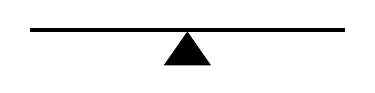
\begin{tikzpicture}
\draw[ultra thick](-2,1) -- (2,1);
\fill[black] (0,0.98) -- (-0.3,0.55) -- (0.3,0.55);
\end{tikzpicture}
\caption{Balanced question}
\label{balanced}
\end{figure}

But as we all know, sometimes questions are biased. For example, the speaker might take one answer to be more likely than another. This leads to an imbalance among the propositions, as in \figref{unbalanced}.

\begin{figure}
%\hspace{0.3cm}\phantom{$\phi$}\\
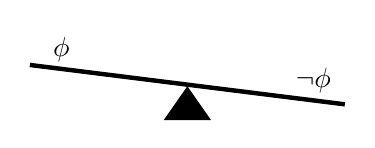
\begin{tikzpicture}[baseline={([yshift={-1ex}]current bounding box.north)}]
\draw[ultra thick](-2,1) -- (2,0.5);
\fill[black] (0,0.73) -- (-0.3,0.3) -- (0.3,0.3);
\node at (-1.6,1.2) {$\phi$};
\node at (1.6,0.8) {$\neg\phi$};
\end{tikzpicture}
\caption{Biased question}
\label{unbalanced}
\end{figure}

There are several interesting questions about this kind of imbalance, including what constitutes the evidence for such an imbalance, whether there are different kinds or different dimensions of tilts, and how can we represent these aspects of meaning.

%\section{Problems for the standard view}

%\subsection{Polar vs. alternative questions}

The existence of biased questions was famously pointed out  by \citet{Bolinger:1978}, who drew attention to the differences between simple polar questions and alternative questions. A polar question like \xref{whetherhelp} is totally normal but an alternative question like \xref{whetherhelpornot} is quite strange, perhaps because the questioner is more interested in the positive answer being true rather than the negative, and this is better expressed by \xref{whetherhelp} than \xref{whetherhelpornot}.

\ea
\ea\label{whetherhelp}
Will you help me?
\ex\label{whetherhelpornot}
Will you help me or not?
\z
\z

Another difference is that polar questions can be conversation starters whereas alternative questions cannot. The sequence in \xref{starter} sounds normal, while that in \xref{nonstarter} sounds odd.

\ea
\ea[]{
Nice to meet you! Do you like to play golf?}\label{starter}
\ex[\#]{
Nice to meet you! Do you like to play golf or not?}\label{nonstarter}
\z
\z

There is also a difference with respect to question complementizers. It seems that embedded polar questions introduced by \textit{if} correlate with simple polar questions, while those introduced by \textit{whether} correlate with alternative questions. Thus, the scenario in \xref{willyoumarryme} is more naturally reported as \xref{ifmarry} than \xref{whethermarry}. 

\ea[]{
John asked Mary: ``Will you marry me?''
}\label{willyoumarryme}
\ex[]{
John asked Mary if she would marry him
}\label{ifmarry}
\ex[?]{
John asked Mary whether she would marry him
}\label{whethermarry}
\z

%John asked Sue if she would marry him is fine, but John asked Sue whether she would marry him seems to indicate that John is neutral about both possibilities, which in this case would make the question sound odd.
Bolinger suggests that the complementizer \textit{whether} is used when the speaker, having already considered the alternative possibilities, is trying to dispassionately gain information about them. We add that this corresponds to our intuition that the use of \emph{whether} in \xref{whethermarry} indicates that John thinks a negative answer is a serious possibility, at least as likely as the positive answer.
%seems to suggest that the subject has no preference with respect to the positive and the negative answer. The complementizer \textit{if}, on the other hand, does not seem to have this inference. %\textcolor{blue}{[DG: My intuition is that the asymmetry here isn't nearly as sharp as for the matrix polar question vs. alternative question. In fact, I think \xref{whethermarry} is basically fine. There is perhaps an intuitive difference, but I wouldn't say that ``whether" conveys that John has ``no preference". It might be that ``whether" conveys that John thinks a negative answer is a serious possibility, though not more likely than the positive answer. Perhaps it conveys that the two answers are equally possible, while ``if" perhaps only draws attention to the positive answer (but doesn't necessarily mean that John is ``biased" for the positive answer).]}

So we see that simple polar questions can highlight one option, while alternative questions highlight both options. We can then ask whether alternative questions are neutral. But as \citet{biezma2019alternative} shows, alternative questions are not neutral. They come with what Biezma calls a `cornering effect': The hearer is forced to give an answer. The question in \xref{marryornot} sounds like it is the last of a series of questions to which the speaker has not gotten a proper answer.

%****DG: I removed the following footnote. This distinction is addressed to a certain extent by Biezma & Rawlins 2017, and Beltrama et al. 2020, who refer to exs like these as "Complement Alternative Questions". Perhaps we'll want to include some discussion of this too, and if so, I can come back and add it. 
%\footnote{This cornering effect seems not to be always present. Consider the following exchange.

%\ex.\label{evenoddexhange}
%\a.[A:] I'm thinking of a number between 1 and 10. Guess which!
%\b.[B:] Is it even or odd?

%Given that a number is either even or odd, B's question is equivalent to an alternative question. However, the question does not have to be read as ``cornering'' A in anyway. \textcolor{blue}{[DG: I thought the cornering effect was only for ``negative alternative questions", which is when the second disjunct is always the negation of the first, e.g. ``or not" or ``or isn't it", etc.]}}

\ea \label{marryornot}
Will you marry me or not?
\z


Let us look at negated questions and the uses of antonyms. Assuming that a bridge is either closed or open, the standard view on questions would assign all of the following sentences the same meaning, namely $\{o, \neg o\}$, where $o$ stands for the bridge is open and $\neg o$ for the bridge is not open, i.e. closed.

\ea\label{bridgequestions}
\ea
Is the bridge open?\label{whetheropen}
\ex \label{openornot}
Is the bridge open or not?
\ex
Is the bridge open or closed?
\ex \label{closed}
Is the bridge closed?
\ex \label{closedornot}
Is the bridge closed or not?
\z
\z

However, the choice of the expression clearly matters \citep{vanrooysafarova2003polar, bustamente2012real, roelofsengool2010disjunctive, trinh2014how}.
In a context where the speaker needs to get to the other side of the river and wants the bridge to be open, and there is no contextual indication as to whether or not it is open, the questions in \xref{bridgequestions} are ranked in the order of most to least appropriate. %, with \xref{whetheropen} being the most appropriate and \xref{closedornot} being the least appropriate. %\textcolor{blue}{[DG: This depends on what else has been said in the context, right? If an interlocutor claims the bridge is closed, and then does or says something to imply it is not closed, the speaker who needs to get to the other side and wants the bridge to be open would then nevertheless find \xref{closedornot} to be most natural, or at least as natural as \xref{whetheropen}.]}

Similarly, in a context where the speaker needs to throw an even number, the utterance in \xref{dice} would be most appropriate with the leftmost choice (\textit{even}) and least appropriate with the rightmost choice (\textit{odd or not}). %\textcolor{blue}{[DG: Suppose the speaker needs an even, but steadfastly believes that their luck is cursed, and therefore an odd number is almost certain. Then ``odd'' is most natural. This comment and my previous comment both are just highlighting the fact that bias has multiple possible sources, as is already mentioned in the chapter above.]}

\ea\label{dice}
I don't dare to look! Is the number even  / $^{?}$even or not / $^{??}$even or odd / \#odd / \#\#odd or not?
\z

However, in both preceding examples, further additions to context can change these intuitions. For example, suppose that in \xref{bridgequestions}, the speaker wants the bridge to be open, but their interlocutor has just indirectly implied that the bridge is closed. In that case, \xref{closed} is most natural. Or suppose the interlocutor ambiguoulsy implies first that it is closed, and then that it is not closed. In that case, \xref{closedornot} would be most natural, despite that the speaker wants the bridge to be open. As for \xref{dice}, suppose the speaker needs an even, but steadfastly believes that their luck is cursed, and therefore an odd number is almost certain. Then asking the question with \textit{odd} is most natural. What this shows is that the contextual factors affecting which question form is most natural are  influenced by multiple competing factors. %All of this shows how sensitive to context the naturalness of the varying forms are. 

How can we differentiate between question meanings so that we can describe their different uses?  Obviously the truth conditional content offered by the theories discussed above does not suffice. We have to look at how these truth conditions are expressed formally. One idea that has been proposed is that different kinds of questions introduce different kinds of discourse referents (DR) (see \citealt{krifka2013} for the role of propositional discourse referents in responses). 

\ea\label{DRs}
\ea \label{rain} 
``Is it raining?'' \hfill $\leadsto$ DR: `it is raining'
\ex\label{notrain}
``Is it not raining?'' \hfill $\leadsto$ DR: `it is not raining'
\ex\label{rainornot}
``Is it raining or not?'' \hfill $\leadsto$ DR: `it is raining', `it is not raining'
\z
\z

As a consequence, these questions would have different discourse potentials. There are other proposals, such as  \citet{roelofsengool2010disjunctive}, which makes it possible to ``highlight'' one of the propositions, leading to a more complex semantic representation. Theories also exist which say the meaning of questions does not have to be balanced. These allow for a monopolar interpretation of questions. Hamblin's semantics, for example, allows for \xref{rain} to denote the set contain only one proposition, namely the proposition that it is raining. The question in  \xref{notrain} would denote the set containing only the proposition that it is not raining. The set denoted by the alternative question in \xref{rainornot} would contain both of these propositions. This is different from the assertion, which is just the proposition, not a set containing the proposition \citep{vanrooysafarova2003polar}.

In commitment space semantics \citep{krifka2015bias}, there is also a way to differentiate between the cases in \xref{DRs}. We assume the common ground, or ``commitment space'', represented by $C$, to be a set of information states, or ``commitment states'', represented by $c$. Each commitment state is a set of possible worlds. The root of C, represented as $\sqrt{C}$, is the set of ``largest'' commitment states, so to speak. %\textcolor{blue}{[DG: In the last draft this said ``smallest'', but I think it should be ``largest'', please double check.]}

\ea\label{rootC}
$\sqrt{C} = \{c \in C \mid \neg\exists c' \in C [c \subset c']\}$
\z

In case of an assertion, say of the proposition that it is raining, represented as $r$, the commitment space C is updated so that it contains only commitment states which entail $r$. 

\ea\label{assertioncommitment}
$C +$ `it is raining' $= \{c \in C \mid c \subseteq r\}$
\z

Questions differ from assertions in that they do not change $\sqrt{C}$, the root of the commitment space. 

\ea\label{questioncommitment}
\ea\label{positivequestioncommitment}
$C +$ `is it raining?' $= \sqrt{C} \cup \{c \in C \mid c \subseteq r\}$
\ex\label{negativequestioncommitment}
$C +$ `is it not raining?' $= \sqrt{C} \cup \{c \in C \mid c \subseteq \neg r\}$
\ex\label{alternativequestioncommitment}
$C +$ `is it raining or not?' $= \sqrt{C} \cup \{c \in C \mid c \subseteq r \vee c \subseteq \neg r\}$
\z
\z

In other words, questions do not add information. Instead, they restrict the continuation of the discourse. As shown in \xref{positivequestioncommitment} and \xref{negativequestioncommitment}, the ``positive'' and the ``negative'' simple polar question restricts $C$ to those $c$ which entail $r$ and $\neg r$, respectively. This is intended to represent the fact that the speaker wants to see if the discourse can continue with the information that it is raining, in the first case, or with the information that it is not raining, in the second case. The alternative question, as shown in \xref{alternativequestioncommitment}, has a yet different meaning from the two simple polar questions.  

Note, however, that this approach would still not capture the distinction between \xref{openornot} and \xref{closedornot}, reproduced below in \xref{openornot2} and \xref{closedornot2}.

\ea\label{openornot2}
Is the bridge open or not?
\ex\label{closedornot2}
Is the bridge closed or not?
\z

The general question, then, is how to represent polar questions properly to capture their different uses.

We now turn to the topic of negation in polar questions \citep{bolinger1957interrogative, Ladusaw:1979, Ladd:1981}. \citet{Ladd:1981} discusses polar questions such as those in \xref{negationquestions}. 

\begin{exe}\label{negationquestions}
\ex\label{lownegation} 
Is it not raining?
\ex\label{highnegation}
Isn't it raining?
\end{exe}

These questions differ with respect to where syntactic negation is. In \xref{lownegation}, it is low, below the subject, while in \xref{highnegation} it is high, above the subject. The low negation question seems to implicate that the speaker wants to be informed as to whether the proposition that it is not raining is true. The high negation question, on the other hand, seems to indicate that the speaker is already inclined to assume that it is raining and wants to confirm this belief.

\citet{Ladd:1981} assumes that high negation questions are actually ambiguous, with both ``outer" and ``inner" interpretations. %Specifically, they allow for a ``low'' interpretation. 
He claims the ambiguity can be resolved by the presence of polarity items like \textit{too} and \textit{either}, which disambiguate the question toward the outer and inner readings respectively. %, or a negative polarity item such as \textit{neither}, which disambiguates the question towards the low reading. %Examples are given in \xref{tooeither}

\begin{exe}\label{tooeither}
\ex\label{too}
Isn't Jane coming too? \hfill $\rightarrow$ outer interpretation
\ex\label{either}
Isn't Jane coming either? \hfill $\rightarrow$ inner interpretation
\end{exe}

A prominent analysis of these facts is proposed by \citet{romerohan2004negative}. %Han:2002a
This analysis assumes a \textsc{verum} operator, whose meaning is a conversational version of the adverbial \textit{for sure}, and whose occurrence is associated with a syntactically preposed high negation. We have the following form-meaning pairs, where $p$ stands for the proposition that Jane is coming. Notice that negation can scope either below or above the \textsc{verum} operator.

\begin{exe}\label{hanromero}
\ex\label{hanromerolowneg}
Is Jane not coming? \\= \textsc{whether}($\neg p$) = $\{\neg p, \neg\neg p\}$ = $\{p, \neg p\}$
\ex\label{hanromerohighnegeither}
Isn't Jane coming (either)? \\ = \textsc{whether}(\textbf{verum}($\neg p$)) = $\{$\textit{for-sure}($\neg p$),  $\neg$\textit{for-sure}($\neg p$)$\}$
\ex\label{hanromerohighnegtoo}
Isn't Jane coming (too)? \\ = \textsc{whether}($\neg$\textbf{verum}($p$)) = $\{$$\neg$\textit{for-sure}($p$), \textit{for-sure}($p$)$\}$
\end{exe}

Romero and Han propose that \textsc{verum} is also present when the question contains the adverb \textit{really}. Thus, \xref{hanromeroreally} ends up having the same meaning as \xref{hanromerohighnegtoo}.

\ea\label{hanromeroreally}
Is Jane really coming?\\
= \textsc{whether}(\textbf{verum}($p$)) = $\{$\textit{for-sure}($p$), $\neg$\textit{for-sure}($p$)$\}$
\z

A similar approach is adopted by \citet{krifka2015bias}, which assumes a commitment operator $\vdash$ that is present in both assertions and questions, and negation can scope either below or above that operator.

\begin{exe}\label{krifkacommitmentoperator}
\ex
$C +$ `is Jane not coming?' = $\sqrt{C} \cup C +$ [Addressee $\vdash$ $\neg p$]\\
$\leadsto$ the speaker is checking whether the addressee is committed to $\neg p$
\ex
$C +$ `isn't Jane coming?' = $\sqrt{C} \cup C +$ $\neg$[Addressee $\vdash$ $p$]\\
$\leadsto$ the speaker is checking whether the addressee is not committed to $p$
\end{exe}

So, there is a wide array of syntactic profiles available for polar question formation: high and low negation, the presence or absence of adverbials like \textit{really}, and also, the presence or absence of bias inducing expressions such as negative polarity items (NPIs). \tabref{tab:1} presents a fine-grained list (probably non-exhaustive) of relevant phenomena (see also the bias profiles discussed in \citealt{gartnergyuris2017delimiting}).

\begin{table}[t]
\fittable{
\begin{tabular}{lll}
\lsptoprule
Example & Abbreviation & Label\\
\midrule
Is it raining? & PQ & positive question\\
Is it not raining? & NQ & negative question\\
Isn't it raining? & HPQ & high negated positive question\\
Isn't it not raining? & HNQ & high negated negated question\\
Is it really raining? & RPQ & \textit{really} positive question\\
It is really not raining? & RNQ & \textit{really} negated question\\
IS it raining? & FPQ & focused positive question\\
IS it not raining? & FNQ & focused negated question\\
Is it REALLY raining? & FRPQ & focused \textit{really} positive question\\
Is it REALLY not raining? & FRNQ & focused \textit{really} negated question\\
It is raining? & DPQ & declarative positive question\\
Is it raining?? & IPQ & incredulity positive question\\
Is it raining or not? & APNQ & alternative question with negation\\
Is the bridge open or closed? & AAntQ & alternative question with antonyms\\
Do you have any potatoes? & npiPQ & positive question with polarity item\\
\lspbottomrule
\end{tabular}
}
\caption{Polar question varieties} \label{tab:1}
\end{table}

Coming back to the topic of negation in questions, one promising approach is to look at contextual features. This goes back to \citet{buringgunlogson2000positive}, which assumes three levels of contextual evidence with respect to the prejacent of a polar question: positive, neutral, and negative. The generalization in \tabref{buringgunlogsongeneralization} is established. 
%\textcolor{blue}{[DG: I'm doubtful that we can get people to adopt the terminology and abbreviations in Table 1.Given that, I think the only reason to  introduce systematic abbreviations here is if we ourselves can consistently use them in the rest of the chapter. But in the following, we display and discuss plots from a few different experiments by other researchers who each have their own different abbreviations, including already ``PPQ" in the next table. So, I suggest that we remove Table 1.]} %Lots of people have worked on this topic now and there is no agreed upon terminology, let alone abbreviations. 

\begin{table}
\begin{tabularx}{\textwidth}{lCCc}
  \lsptoprule
\multirow{2}{*}{contextual evidence} & \multirow{2}{*}{PPQ} & \multicolumn{2}{c}{HPQ} \\
\cmidrule{3-4}
 & {} & high reading & low reading \\
   \midrule
positive & \ding{51} & \ding{55} & \ding{55}\\
neutral & \ding{51} & \ding{51} & \ding{55}\\
negative & \ding{55} & \ding{51} & \ding{51}\\
  \lspbottomrule
\end{tabularx}
\caption{\quotecite{buringgunlogson2000positive} generalization} \label{buringgunlogsongeneralization}
\end{table}

\largerpage[2]
The contextual evidence is ``positive'' if it supports the prejacent, ``neutral'' if it neither supports nor speaks against the prejacent, and ``negative'' when it speaks against the prejacent. Thus, even PPQs are not neutral, in the sense that there are contexts where they cannot be used, namely those with negative evidence. Note that \citet{buringgunlogson2000positive} take HPQ with a low negation to mean the same as NQ. Thus, \xref{hpqlow} and \xref{nq} would be equivalent in this approach.

\ea
\ea\label{hpqlow}
Isn't Jane coming either?
\ex\label{nq}
Is Jane not coming either?
\z
\z

The first experimental work on this topic is done by \citet{roelofsen2013}. This is a rating experiment, which contrasts prior speaker's belief (SB) with positive, neutral, and negative contextual evidence (CE). The experiment yields interesting results about the different uses of positive, high negation, and low negation questions as presented in \figref{pic:123}.
%\textcolor{blue}{[DG: I haven't read this paper, and I guess I need to. The results in (24) and (25) make no sense to me. Either I've misunderstood or there was a problem with the stimuli. Note also that we don't actually discuss this data below, which makes me wonder if we should include these plots. It seems the main reason for mentioning this paper is to discuss the preference rules and OT below, maybe we could just do that directly.]}

\begin{figure}
\subfigure[PPQs]{
\includegraphics[width=.45\textwidth]{figures/Roelofsen-PPQ.pdf}
}
\subfigure[HNPQ]{
\includegraphics[width=.45\textwidth]{figures/Roelofsen-HNPQ.pdf}
}
\subfigure[LNPQ]{
\includegraphics[width=.45\textwidth]{figures/Roelofsen-LNPQ.pdf}
}
\caption{\quotecite{roelofsen2013} experimental results}
\label{pic:123}
\end{figure}


These uses were described in terms of various preference rules. An example of such a rule is ``ask only if needed''. According to this rule, there is no need to ask any question if speaker's belief and contextual evidence coincide. Another rule is ``avoid reversing processes'', which says that it would be strange to ask whether $\neg p$ is true when the speaker's belief or the contextual evidence supports $p$. Yet another rule is ``use the least marked form'', which would prefer a positive question to a negative or an alternative question, for example. We note that these rules resemble constraints in bidirectional optimality theory (OT) in pragmatics, hence raise the question whether bidirectional OT should be employed in analyzing biased questions. We believe this perspective is promising.

It has become consensus to assume three levels -- positive, neutral, negative -- for both contextual evidence and prior speaker's belief, or ``evidential bias'' and ``epistemic bias'', which are terms proposed by \citet{sudo2013biased} which have gained some currency. We could let SB stand for prior speaker's belief and CE for contextual evidence, and use $+$, $0$ and $-$ to represent the three levels positive, neutral, and negative. %Furthermore, we could adopt the convention of placing. 
Bias profiles of questions could then be represented more succinctly. For example, [SB$-$, CE$+$] is a question with negative prior speaker's belief and positive contextual evidence, and [SB$0+$, CE$-$] would be a question with neutral or positive prior speaker's belief and negative contextual evidence. If we adopt the convention of placing the value for SB to the left of that for CE, the profiles can be represented even more economically. Thus, [SB$-$, CE$+$] can be shortened to [$-$/$+$] and [SB$0+$, CE$-$] to [$0+$/$-$]. %\textcolor{blue}{[DG: It looks like maybe we get some use of these abbreviations some of the tables below; maybe we should introduce those abbreviations there.]} 

\citet{domaneschi2017bias} present further experimental results. Tests were conducted on high negation questions (HiNQ), low negation questions (LowNQ), positive question (PosQ), and positive question with \textit{really} (ReallyPosQ). The object languages were English and German. Participants were given a selecting task, where they had to pronounce their option. The main results are presented in \figref{fig:chart23}. %\textcolor{blue}{[DG: With this data as well, we're not really discussing it. Perhaps that is fine, and the idea here is just to provide the reader with the results themselves. But then we need to explain the condition labels on the X axis. If we decide to keep these plots in here, I am happy to add explanations for the condition labels.]}

\begin{figure}
% \begin{subfigure}{0.43\textwidth}\centering
\includegraphics[height=.45\textheight]{figures/Domaneschi-1.pdf}
%\caption{\color{red}{Please provide a caption}}
%\label{fig:chart2}
% \end{subfigure}
% \begin{subfigure}{0.41\textwidth}\centering
\includegraphics[height=.45\textheight]{figures/Domaneschi-2.pdf}
%\caption{\color{red}{Please provide a caption}}
%\label{fig:chart3}
% \end{subfigure}
\caption{\quotecite{domaneschi2017bias} experimental results}
\label{fig:chart23}
\end{figure}

A recurring question is whether syntactically high negation questions (HPQs) are semantically ambiguous. \citet{Ladd:1981} claims that they are; \citet{sailor2012remarks, anderbois2019, goodhue2022} all argue that they are not. It should be pointed out, however, that Sailor's data can be accounted for by assuming that for English, HPQs are ambiguous while NQs are not, and for German, the opposite is the case. %\textcolor{blue}{[DG: I'm not sure what is meant by this claim. In my paper, I make a concerted effort to show that the data speaks against the existence of an ambiguity in American English HPQs.]}

\ea English
\ea Isn't there a train in the early morning? \hfill $\neg Qp$ / $Q\neg p$
\ex Is there no train in the early morning? \hfill $Q \neg p$
\z

\ex German
\ea Gibt es hier nicht einen Zug am Morgen? \hfill $\neg Qp$
\ex Gibt es hier keinen Zug am Morgen? \hfill $Q\neg p$ / $\neg Qp$
\z
\z

How can we explain this difference between English and German? Suppose we say that in the [SB$+$, CE$-$] scenario, the wide-scope negation reading is the best. If we then assume that in German this wide-scope interpretation can also be expressed by a syntactically low negation, we can explain why there is more uses of this option in German.

The interesting issue here, therefore, is whether there are different readings of high negation questions and low negation questions. 

\citet{sudo2013biased} looks at the Japanese counterparts of positive questions (PQs), high negation questions (HQs), and low negation questions (NQs). 

\ea
\gll Mary-ga kita $\{\emptyset$ / no / desho$\}$\\
Mary-NOM came\\ 
\glt `Did Mary come' \hfill PQ 
\ex
\gll doko-ka nihon-shoku nai?\\
where-\textsc{ka} Japanese-food not.exist\\
\glt `Isn't there some Japanese restaurant?' \hfill HQ
\ex
\gll doko-mo nihon-shoku nai?\\
where-\textsc{mo} Japanese-food not.exist\\
\glt `Isn't there any Japanese restaurant?' \hfill NQ
\z

Sudo treats epistemic and evidential bias, at different levels, as features which can be combined in different ways as presented in \tabref{figtab:chart45}. \citet{gyuris2017new} looks at three different types of polar questions in Hungarian as presented in \tabref{figtab:chart6}.

\begin{table}
% \includegraphics[width=.5\textwidth]{figures/Sudo-1.pdf}
\caption{\quotecite{sudo2013biased} taxonomy}
\label{figtab:chart45}
\begin{tabularx}{\textwidth}{XXXc}
\lsptoprule
 Question type & Epistemic &  Evidential & Short\\
 \midrule
 PQ            & none      &  not negative &  --0+/0+\\
 HQ            & positive  &  not positive & +/--0\\
NQ             &  positive & neutral        & +/0\\
\lspbottomrule
\end{tabularx}
\end{table}

\begin{table}
% \includegraphics[height=.5\textheight]{figures/Gyuris-1.pdf}
\caption{\quotecite{gyuris2017new} taxonomy}
\label{figtab:chart6}
\fittable{
\begin{tabular}{lccc}
\lsptoprule
                                  & -e-interrogative &  $\wedge$-interrogative  & $\wedge$-declarative\\
                                  \midrule
Neutral information question, (11)& {\langscicheckmark} & {\langscicheckmark} & {\langscicross}\\
Grounding question, (12)          & {\langscicross}     &\%                   & {\langscicheckmark}\\
Indirect Request                  & {\langscicross}     &  {\langscicheckmark}& {\langscicross}\\
Indirect offer, (14)              & {\langscicheckmark} &  {\langscicheckmark}& {\langscicross} \\
 Conversation  starter, (15)      & {\langscicross}     &  {\langscicheckmark}& {\langscicross}\\
Pedagogical question              & {\langscicheckmark} & {\langscicheckmark} & {\langscicross}\\
Monological question              & {\langscicheckmark} & {\langscicheckmark} & {\langscicross}\\
Exam question, (18)               & {\langscicheckmark} & {\langscicheckmark} & {\langscicross}\\
Rhetorical question, (19)         & {\langscicheckmark} & {\langscicheckmark} & {\langscicross}\\
\lspbottomrule
\end{tabular}
}
\end{table}

\begin{table}
% \includegraphics[height=.17\textheight]{figures/Gyuris-2.pdf}
\caption{\quotecite{gartnergyuris2017delimiting} bias profiles}
\label{figtab:chart7}
 \begin{tabularx}{.8\textwidth}{Xcc}
 \lsptoprule
 Question type & Speaker belief & Current evidence\\
 \midrule
  ePQ          &                 &0                        \\
 $\wedge$PQ          &                 &0, for some speakers --  \\
 $\wedge$DPQ         &                 &+                        \\
 eHQ           &   +             &0                        \\
 $\wedge$HQ          &   +             &--0                      \\
 $\wedge$NQ          &   +             &--                       \\
 $\wedge$DNQ         &                 &--                       \\
 \lspbottomrule
  \end{tabularx}
\end{table}

\citet{gartnergyuris2017delimiting} look at possible bias profiles (see \tabref{figtab:chart7}). There are $7 \times 7 = 49$ possible SB/CE combinations. When we consider the three types of questions (PQ, HQ, NQ), we end up with $7^3 \times 7^3 = 117649$ possibilities, which is an astonishing number due to combinatorial explosion. But one can reduce the number of possibilities by certain general principles. %\textcolor{blue}{[DG: Like what?]}
For example, a principle of Markedness could favor non-negated questions over negated ones so that they are also used for neutral questions (cf. also \citealt[230]{trinh2014how}). 

Let us now turn to the topic of NPIs in questions \citep{Ladusaw:1979, Kadmon:1993, krifka1995semantics, vanRooy:2003}. It has been observed that NPIs do not occur in declarative questions. Since declarative questions presumably have a [$-0+$/$+$] profile, in case of rising contour, or a [$-$/$+$] profile, in case of incredulity contour, questions with NPIs must have a [*/$-$0] profile. Questions with strong idiomatic NPIs (i.e. minimizers) appear to have a [$-$/$-0$] profile, meaning their use requires that the speaker not believe and the context not have evidence for the prejacent.

\ea
\ea
Did John do anything to help?
\ex
Did John lift a finger to help?
\z
\z

\citet{asherreese2005negative} account for NPIs in questions by assuming that such questions actually come with a negated assertion, which is what licenses the NPI. Another way to explain the felicity of NPIs in questions is by appealing to the fact that a question denotes a set containing a proposition and its negation, and it is the negated proposition which licenses the NPIs. The unacceptability of NPIs in declarative questions can then be explained by saying that these questions are monopolar: they denote sets containing only one proposition. \citet{guerzoni2014} account for the distribution of NPIs in questions by claiming that many questions contain covert disjunction with a covert negation that licenses the NPI. On this view, it could be argued that declarative questions fail to license NPIs because they lack covert disjunction and negation. 

\citet{krifka1995semantics} and \citet{vanRooy:2003} propose that NPIs in questions create a more equal distribution of the likelihood of both options by way of widening the meaning of the NP complement. Thus, \textit{potatoes} in \textit{any potatoes} would denote a superset of \textit{potatoes} in \textit{some potatoes}. Strong NPIs would increase the chance of the positive answer being true, and this is a strategy for showing preference for the negative answer. It is, however, not clear how to represent the bias which comes about by way of (strong) NPIs with the features that we have discussed. %\textcolor{blue}{[DG: Should we also cite Guerzoni \& Sharvit here about NPIs in questions?  I haven't read the paper closely, perhaps someone with more expertise on NPIs in Qs has an opinion...]}

We believe that a distinction has to be made within the category of contextual evidence (CE). Specifically, we need to differentiate between CE which is factual and CE which is infered from what the addressee says. %\textcolor{blue}{[DG: This and the following idea about assertions are both very interesting, but also terse enough that I'm not sure what to make of them. Why does this distinction have to be made? Do we think it affects what the speaker bias profile of the question can be? Perhaps it does, but I think it requires demonstration.]}

\ea Factual
\ea A: Coming in with a dripping raincoat
\ex B: Is it really raining outside?
\z
\z

\ea Addressee's belief
\ea A: The rain is bothering me!
\ex B: Is it really raining outside?
\z
\z

This leads us to the question of when an assertion is biased. Presumably, an assertion is biased if the speaker's belief supports the asserted proposition, there is no contextual evidence against it, but the addressee does not believe it yet. We can enrich our feature notation by placing the addressee's belief in brackets.

\ea
It is raining \hfill [$+$/$0+$] or [$+$/$0+(-0)$]
\ex
It isn't raining \hfill [$-$/$-0$] or [$-$/$-0(0+)$]
\ex
Really, it is raining \hfill [$+$/$0+(-)$]
\z

Other relevant topics include in-situ wh-question \citep{biezma2019alternative}, assertions with question tags, and miratives \citep{delancey1997mirativity, bustamente2012real}. 

Last but not least, we would like to emphasize the importance of prosody. In this connection, \citet{Bartels:1999} should receive mention. We would draw attention to the discussion on ``falling'' declarative questions, i.e. those that are not marked by rising contour. Other works on prosody and bias include \citet{gricesavino2003map}, \citet{kugler2004dialectal}, and \citet{arnhold2021}. 

\section{The contributions to this volume}

In their chapter \textit{Biased questions and modal ranking}, Alda Mari and Anastasia Giannakidou point out that questions share a semantic feature with epistemic modals: They are non-veridical in the sense that they do not entail that their prejacent proposition $p$ is true. The authors suggest that questions with negative and positive bias lie on a continuum between regular questions and assertions, and that they share this property with weak and strong epistemic modals that modify assertions. Both questions and epistemically modified statements require that the modal base of the speaker contains both $p$ and $\neg p$ worlds (the ``nonveridicality axiom of modals and questions''). But questions and epistemically modified statements differ insofar as only the latter have truth conditions and can be said to be true or false. The authors discuss three empirical domains. First, \textit{really}-questions are analyzed as marking a genuine interest of the speaker and having a negative bias. They provide an account of \textit{really} in which this adverb points to a different ranking of propositions between the assumptions of the speaker and evidence of the context, with reference to experimental work on \textit{wirklich} in German. They show that negatively biased questions ask for stronger confirmation; a response like \textit{I think so} is felt to be insufficient. The second domain are questions with high negation and low negation with a positive bias, which are related to assertions with the strong modal \textit{must} that also expresses a positive bias. The third domain are \textit{reflective} or \textit{conjectural} questions marked with weak epistemic modals, such as \textit{might}. They observe that the modals must be weak, and argue that they widen the modal base, enlarging the range of possibilities, thus unearthing remoter ways in which a proposition may be true. As for assertions, the authors suggest that they are only added into the common ground when not modalized.    


In her chapter, \textit{Evidential bias across clause types}, Beste Kamali compares English rising declarative questions, known to express a positive bias towards their proposition, with a polar question type in Turkish. In this language, polar questions are always marked by a particle \textit{\textsc{mi}} that is attached to a constituent of the sentence, then often marking the focus of the question, or after the (typically final) finite verb of the sentence, indicating a polar question without focus. However, when \textit{\textsc{mi}} attaches to the direct object, focus may project to the whole sentence. There are subtle differences between such sentences and sentences where \textit{\textsc{mi}} is attached to the final verb. In particular, the object-\textit{\textsc{mi}} sentences have a reading that has a similar bias to English rising declarative questions, insofar as they also require a positive evidential bias. However, a careful examination in a battery of tests reveals interesting differences: First, object-\textit{\textsc{mi}} questions are classified as ``questions'' in the object language, different from English (cf. \textit{One question remains: Did Ali make dinner?} / \textit{\#Ali made dinner?}). They do not allow for modal adverbials, different from English (cf. \textit{You certainly made dinner?}). And they can be embedded by rogative predicates, again different from English (*\textit{She asked Ali made dinner?}).  Hence, object-\textit{\textsc{mi}} questions achieve their positive bias in ways quite different from English declarative questions. According to the proposed analysis, they both are monopolar, in contrast to regular polar questions and verb-final \textit{\textsc{mi}}-questions, which are analyzed as bipolar. Their differences derive from the fact that they are syntactically and semantically different clause types. The author also draws in evidence from Hungarian and Japanese that show similar question types as Turkish object-\textit{\textsc{mi}} questions. 


In their chapter, \textit{The contribution of intonation in the conveyance of question bias}, Riccardo Orrico, Cristel Portes, Mariapaola D'Imperio provide a comprehensive overview of the role of intonation in the expression of question bias. They begin with a review of the literature on intonation patterns and the different dimensions of meaning they can express. This review is followed by a discussion of two recent experimental studies conducted by the authors themselves. Throughout the chapter, the authors address three main questions about the relationship between phonetic cues and speaker meaning: the kinds of meanings that can be expressed by intonation, the intonational cues that convey these meanings, and the degree of variation within the linguistic population. After a general overview, they provide a detailed comparison of the means used by Italian and French speakers to express question bias. They argue that the way in which meaning is encoded in intonation patterns is not universal. Their study shows that different languages have their own specific cues to express specific meanings.  

In their chapter, \textit{Negative Polar Questions in Russian: Question bias and question concern}, Sophie Repp and Ljudmila Geist study the appropriateness conditions of yes--no questions containing the particles \textit{razve} and \textit{neu\v{z}eli}, both of which can be translated as \emph{really}. In their analysis, they distinguish between the bias profile of a question and the \textit{question concern}. The \textit{bias profile} is defined by the question's \textit{epistemic} and \textit{evidential} bias \citep[following][]{s3budo201iased}, where the former refers to the speaker's prior beliefs and the latter to contextual evidence that may or may not conflict with the speaker's beliefs. By \textit{question concern} they refer to the purpose of checking or rejecting the prejacent of a question, or its negation. Repp and Geist assume that the appropriateness of different types of polar questions depends on their bias profile and their concern. They demonstrate the usefulness of this asumption for polar questions in English, and then extend the analysis to polar questions in Russian with or without particles \textit{razve} and \textit{neu\v{z}eli}. Repp and Geist show that polar questions with \textit{razve} and \textit{neu\v{z}eli} do not differ in their bias profile but in their ability to check the truth of the proposition which is favoured by the question's epistemic bias. Repp and Geist support their analysis by a corpus study and two experimental investigations. They further provide a semantic explanation for the difference between \textit{razve} and \textit{neu\v{z}eli} in terms of their consistency with inner and outer negation.

In their chapter, \textit{Bias in Tag Questions}, Corey Bill and Todor Koev study constructions consisting of a VP-eliptical yes/no question which is ``tagged'' onto an ``anchor'' declarative sentence of the opposite polarity, as exemplified by \textit{it's raining, isn't it?} and \textit{it's not raining, is it?}. It has been observed that tag questions give rise to the inference that the speaker is ``biased'' toward the anchor, i.e. that she believes the proposition it expresses to be true. Bill and Koev propose to describe such biases in terms of two parameters: (i) whether they are weak or strong, and (ii) whether they are optional or obligatory. They devise diagnostics to test these distinctions, and advance an analysis to derive the observations from syntactic and phonological properties of tag questions.

In their chapter, \textit{Contextual Bias and the Landscape of Mandarin Polar Questions}, Yurie Hara and Mengxi Yuan discuss \textit{ma}-questions and A-not-A questions in Mandarin Chinese. They present the following observations: (i) positive \textit{ma}-questions can be used in either neutral or positively biased contexts; (ii) negative \textit{ma}-questions can only be used in negatively biased contexts; (iii) A-not-A questions can only be used in neutral contexts. They then argue that it is contextual bias, not speaker's bias, which is instrumental for an analysis of this distribution. The concept of ``contextual bias'' is defined in terms of subjective probability and \citeauthor{farkasbruce2010reacting}'s (\citeyear{farkasbruce2010reacting}) Table model.

In their chapter, \textit{What can Cantonese sentence-final particles tell us about rhetorical questions?}, Angelika Kiss, Roger Yu-Hsiang Lo, and Justin R. Leung discuss three kinds of questions: (i) information seeking questions (ISQ), (ii) rhetorical question with empty set answers (RQ–), and (iii) rhetorical questions with non-empty set answers (RQ+). It uses the framework of inquisitive semantics to argue that these are in fact natural classes in terms of informativity and speaker's commitment. Moreoever, ISQ and RQ– make up a subclass in this three membered group. An perception experiment is then presented whose result shows that the semantic distinctions are also reflected prosodically in Cantonese, specifically in distinctions with respect pitch contour and length of the final sentence particle.

In his chapter, \textit{A note on bias and polarity in Vietnamese}, Tue Trinh discusses the distribution of two types of NPIs across two types of polar questions. NPIs in Vietnamese come in two morphological variants, one simple and one complex. Among polar questions in this language, Trinh distinguishes between yes/no questions and agreement questions. The observation is that complex NPIs are acceptable in yes/no questions but deviant in agreement questions, and in yes/no questions, complex NPIs give rise to negative bias while simple NPIs do not. The analysis Trinh proposes for this fact assumes that complex NPIs require a covert EVEN in the structure, and that agreement questions contain a covert evidential marker. 


%In their chapter, {\bf Psycholinguistic processing tasks and the study of question bias}, E Jamieson and Vinicius Macuch Silva approach the issues related to biased questions from the experimental perspective. The chapter discusses different theoretical approaches to biased questions, overview of Psycholinguistic investigation on the topic, as well as what data from the experimental studies provide for the ongoing discussion, contrasting with the more traditional introspective data and judgments. In addition, Jamieson and Silva provide concrete suggestions and guidance regarding the aspects of experimental set-up, providing important resources for future researches.

Much of the study on biased questions has been based on the introspective intuition from different languages. In this chapter, \textit{Psycholinguistic processing tasks and the study of question bias}, E Jamieson and Vinicius Macuch Silva provide another dimension: how can we investigate the issues related to biased questions from an experimental perspective? The chapter discusses different theoretical approaches to biased questions, an overview of psycholinguistic investigations on this topic, as well as the contribution of experimental data to the ongoing discussion and understanding of polar questions. In addition, Jamieson and Silva provide concrete suggestions and guidance regarding the aspects of experimental set-up, providing important resources for future researches.


Hungarian interrogatives are marked with a special suffix. In her chapter, \textit{Marking the type of speaker bias: Hungarian \textit{nem-e} interrogatives}, Gyuris examines a particle \textit{nem-e}, which consists of a negation and an interrogative marker. This particle has not been investigated before, and naturally, Gyuris is the first to describe the different characteristics that the particle exhibits, and to a semantic account.  Gyuris first discusses the meaning contribution and the distribution of the canonical question particle \textit{-e}, showing the interaction between its meaning and biases. She then discusses the data on \textit{nem-e}, and reveals that their meaning and distributional pattern reveal cross-dialectal variation: \textit{nem-e} gives rise to the outside negation reading but not inside negation reading, and is incompatible with different types of biases.
After identifying different uses of \textit{nem-e}, Gyuris provides analyses of the particle, which predicts and accounts for their distribution. The chapter is a welcome addition to our understanding of biased questions.


In their chapter, \textit{Children's acquisition of English ``high'' negation: A window into the logic and composition of bias in questions}, Rebecca Woods and Thomas Roeper investigate the production of English nuclear negative tag structures and negative questions, produced by children and adults. They argue that the structures of negative tags and negative questions are distinct, the former being simple speech acts that are complex at the clausal level. The negative questions, on the other hand, involve an interrogative clause, scoped over by metalinguistic negation and a question operator. Woods and Roeper provide a new type of evidence for their analysis, providing making valuable (and novel) empirical contribution to the volume (suggetion)s.

In his chapter, \textit{Everything that rises must converge: Toward a unified account of inquisitive and assertive rising declaratives}, Daniel Goodhue investigates the relationship between rising declarative clauses that are used to ask questions, and those that are used to make assertions. English matrix declaratives with a final rising intonation typical of polar questions are frequently used as a biased question: they convey that there is contextual evidence in favor of the proposition denoted by the declarative. However, some rising declaratives assert the content of the declarative, while raising a second issue. Goodhue offers a unified account of rising declaratives that seeks to explain both of these kinds of uses while positing unitary meanings for clause types and intonations. Achieving this goal depends the view that illocutionary force is not determined by clause type and intonation. Instead, clause type and intonation are proposed to merely constrain what a speaker could intend to do with them; pragmatic inference then plays a key role in enabling an audience to uncover the speaker's illocutionary intention. The proposed account enables a derivation of assertive force. 

\printbibliography[heading=subbibliography,notkeyword=this]
\end{document}

\chapter{A feature-based approach to functional left peripheries} \label{ch:2}
\section{Introduction} \label{sec:2introduction}
%\chaptermark{A feature-based approach}
In this chapter, I am going to present the basic assumptions concerning a minimal, feature-based approach to the syntax of functional left peripheries, showing that the proposed analysis applies to various clause types, in each case correctly predicting the surface order of clause-typing elements appearing in combinations. Since the relevant combinations are restricted to embedded clauses in Germanic languages, this chapter will be focusing on subordinate clauses, even though, as will be indicated, the analysis is also applicable to main clauses. In particular, I will be arguing against cartographic approaches, showing that clause-typing elements appearing on functional left peripheries are not in a one-to-one relationship with syntactic features, and the assumption that there are designated projections for the various semantic properties is fundamentally flawed. Instead, I propose that functional left peripheries are as minimal as possible, and multiple projections are generated when the relevant semantic properties cannot be marked in a single projection; whether this is the case is ultimately dependent on the lexical properties of the individual clause-typing elements. To put the analysis into an appropriate context, I am first going to review some previous proposals of relevance: the papers discussed here are not meant to be a representative summary of the state of the art but they are selected analyses that have been particularly influential and/or are of particular interest for the analysis pursued here.

This chapter is structured as follows. Section \ref{sec:2previous} provides an overview of some previous accounts. Section \ref{sec:2introducing} introduces the basic ideas regarding the flexible approach to left peripheries put forward in this book. This basic proposal will be refined with more details in the subsequent sections: \sectref{sec:2interrogatives} discusses embedded interrogatives, \sectref{sec:2relative} discusses relative clauses, and \sectref{sec:2degree} discusses embedded degree clauses. These clauses types will be dealt with in more details in the rest of this book.

\section{Previous accounts} \label{sec:2previous}
\subsection{The problems to be discussed} \label{sec:2problems}
In current minimalist theory, the Complementiser Phrase (CP) is responsible for typing clauses and for encoding finiteness in finite clauses.\footnote{See, for instance, \citet[283]{rizzi1997}, for anchoring finiteness in the CP-system. Note that finiteness is ultimately inherited from the inflectional system (see \citealt{chomskylasnik1977} and \citealt{denbesten1983}). This also means that a clause can be finite without a CP layer, as is the case for English main clause declaratives, which are standardly assumed to be TPs.} Apart from complementisers, various operators can appear in this domain. Consider:

\ea
\ea I wonder \textbf{if} Ralph has arrived. \label{englishif}
\ex I wonder \textbf{whether} Ralph has arrived. \label{englishwhether}
\z
\z

In (\ref{englishif}), the element \textit{if} is a complementiser and it types the subordinate clause as interrogative. In (\ref{englishwhether}), there is no overt complementiser but the operator \textit{wheth\-er} is present. In such cases, it is generally assumed that the zero complementiser types the clause, yet a sound model of the CP-periphery must also clarify the role of the overt operator in (\ref{englishwhether}), especially because its appearance in dialects like Standard English is tied to the absence of the overt complementiser:

\ea[*]{I wonder \textbf{whether if} Ralph has arrived. \label{whetherifch2}}
\z

On the other hand, the CP is not restricted to hosting a single overt element: depending on the particular construction and the dialect, multiple elements may appear in the CP-domain. This is illustrated by (\ref{englishdfc}) for non-standard English and by (\ref{norwegiandfc}) for Norwegian\footnote{The Norwegian data stem from the cross-Germanic survey of \citet[175]{bacskaiatkaribaudisch2018}. Both of the informants marked the sentence in (\ref{norwegiandfc}) as grammatical.}:

\ea \label{dfc}
\ea[\%]{ I wonder \textbf{which book that} Ralph is reading. \label{englishdfc}}
\ex[]{ \gll Peter spurte \textbf{hvem} \textbf{som} likte bøker. \label{norwegiandfc}\\
Peter	asked.\textsc{3sg} who	that liked books\\
\glt `Peter asked who liked books.'}
\z
\z

A proper formal account of the CP-domain must be able to condition when multiple overt elements are allowed and when not. Further, it must be clarified whether the appearance of several overt elements requires multiple CP projections, and in cases where it does, how word order restrictions can be modelled. The generation of multiple functional layers is in principle possible, yet it should be appropriately restricted to exclude the generation of superfluous layers that are empirically not motivated. This question is likewise relevant in cases involving a single overt C-element, since then the question arises whether and to what extent covert elements and phonologically invisible projections are present.

Apart from the exact position of various elements in the CP, their function(s) must also be addressed. For instance, interrogative complementisers regularly encode finiteness as well, imposing finiteness restrictions on the complement TP. Consider:

\ea \label{ifwhether}
\ea[]{I don't know \textbf{if} I should call Ralph. \label{iffinite}}
\ex[]{I don't know \textbf{whether} I should call Ralph. \label{whetherfinite}}
\ex[*]{I don't know \textbf{if} to call Ralph. \label{ifnonfinite}}
\ex[]{I don't know \textbf{whether} to call Ralph.  \label{whethernonfinite}}
\z
\z

\begin{sloppypar}
In (\ref{iffinite}), the complementiser \textit{if} introduces a finite embedded interrogative clause, and as the ungrammaticality of (\ref{ifnonfinite}) shows, it is incompatible with a non-finite clause, suggesting that it encodes finiteness apart from the interrogative property. By contrast, the operator \textit{whether} is compatible with both a finite clause, as shown in (\ref{whetherfinite}), and with a non-finite clause, as shown in (\ref{whethernonfinite}), indicating that the overt marking of interrogativity is not incompatible with a non-finite clause in English. Since \textit{whether} is not specified for finiteness, it should be clear that finiteness is specified by some other element in (\ref{whetherfinite}); the question is whether there is a separate element encoding finiteness in (\ref{iffinite}) as well and, if so, how the restriction of \textit{if} to finite clauses can be explained.
\end{sloppypar}

Finally, the function(s) of various left-peripheral elements must be clarified also because there are some non-trivial combinations in which elements seem to be largely similar, as in the non-standard German example in (\ref{alswie}) below:

\ea
\ea[\%]{\gll Ralf ist größer \textbf{als} \textbf{wie} Maria. \label{alswie}\\
Ralph is taller than as Mary\\
\glt `Ralph is taller than Mary.'}
\ex[]{\gll Ralf ist größer \textbf{als} Maria. \label{als}\\
Ralph is taller than Mary\\
\glt `Ralph is taller than Mary.'}
\ex[\%]{\gll Ralf ist größer \textbf{wie} Maria. \label{wie}\\
Ralph is taller as Mary\\
\glt `Ralph is taller than Mary.'}
\ex[]{\gll Ralf ist so groß \textbf{wie} Maria. \label{wieequat}\\
Ralph is so tall as Mary\\
\glt `Ralph is as tall as Mary.'}
\z
\z

In (\ref{alswie}), the elements \textit{als} and \textit{wie} both seem to mark the comparative nature of the clause, whereby single \textit{als} is the comparative particle in Standard German comparatives, see (\ref{als}), and single \textit{wie} is the comparative particle in equatives, see (\ref{wie}), and in certain dialects also in comparatives, see (\ref{wieequat}). In such cases, the question is to what extent there is genuine doubling at hand and how it can be modelled.

\subsection{The cartographic approach -- \citet{rizzi1997, rizzi2004}} \label{sec:2rizzi}
I will start reviewing the relevant literature with Rizzi's work, since it is generally taken to be the foundation of cartographic approaches.\footnote{The original model was extended by later work by several scholars working in the cartographic framework, such as \citet{frascarelli2000, frascarelli2008}, \citet{paoli2003diss, paoli2007}, \citet{benincapoletto2004}, \citet{polettopollock2004}, \citet{beninca2006}, \citet{frascarellihinterhoelzl2007}, \citet{cinquerizzi2008, cinquerizzi2009}, \citet{bocci2013}, \citet{polettozanuttini2013}, \citet{bianchiboccicruschina2017, bianchiboccicruschina2018}, \citet{boccicruschina2018}, \citet{rizzibocci2017}, \citet{boccicruschinarizzi2021}, \citet{boccibianchicruschina2021}. As these works do not fundamentally differ from the original idea in spirit (in fact, they explicitly adopt Rizzi's framework), the concerns expressed here in connection with \citet{rizzi1997, rizzi2004} also apply to them. The aim of this section is not to provide an overview of the cartographic approach but rather to focus on the motivating factors underlying the original idea, as well as potential problematic points.} While his model was primarily developed for Romance languages (and for Italian in particular), the model implies a universal applicability; indeed, the Germanic left periphery has been analysed in a (partial) cartographic fashion as well (see, for instance, \citealt{haegeman2007, haegeman2012, haegeman2013, haegeman2014, haegeman2017} and \citealt{hinterhoelzlpetrova2010, hinterhoelzlpetrova2010focus}).\footnote{While there are certainly differences in the exact combinations that are attested in the two language groups, the similarities are altogether overwhelming. In both Germanic and Romance, clause-typing elements such as complementisers and operators (e.g. interrogative and relative operators) can occur in the left periphery, as well as other XPs that are fronted to the CP-domain without encoding clause type. In \chapref{ch:6}, I argue that XP-fronting is largely due to an unspecified [edge] feature. In this respect, Germanic seems to be more restrictive, as there is generally only a single XP fronted to the CP (leading to the canonical V2 pattern); however, this is not necessarily the case, as will be discussed in connection with V3 patterns in \chapref{ch:3}. Note also that while the Romance left periphery appears to be able to host multiple fronted XPs, fronting is not the only option for marking information structure: in fact, as shown by \citet{sameklodovici2015} for Italian, contrastive focus occurs in situ by default.}

The basic observation underlying Rizzi's model is that while in the 1980s the layers VP, IP and CP were taken to be composed of single projections each, there is evidence for there being a more intricate structure underlying these domains, as was already established for the VP and the IP\footnote{In this book, I will restrict myself to the discussion of cartographic approaches to the CP-domain; note that such approaches have also been proposed for the IP-domain, see, for instance, \citet{cinque1999}, \citet{belletti2004}, \citet{cardinaletti2004}.} towards the end of the 1980s (\citealt[281]{rizzi1997}). Essentially, \citet{rizzi1997} assumes that the same holds for the left periphery of the clause, that is, the domain above IP.

According to \citet[283]{rizzi1997}, the CP-domain has two major functions. On the one hand, it relates the clause to the outside, that is, either to a superordinate structure or, in the case of root clauses, to the articulation of the discourse. This kind of information expresses whether the clause is, for instance, a question or a declarative, and is referred to as the clausal Type by \citet{cheng1991diss} and the specification of Force by \citet{chomsky1995}, whereby \citet[283]{rizzi1997} adopts the latter term. As pointed out by \citet[283]{rizzi1997}, ``Force is expressed sometimes by overt morphological encoding on the head (special C morphology for declaratives, questions, relatives etc.), sometimes by simply providing the structure to host an operator of the required kind, sometimes by both means''. The last option is considered to be rare by \citet{rizzi1997}, who attributes this to economy principles on representation, following \citet{cheng1991diss} among others.

On the other hand, the CP-domain has an effect on its complement domain, namely the IP, and \citet[283--285]{rizzi1997}, following \citet{holmbergplatzack1988}, among others, assumes that the CP is responsible for encoding finiteness. That is, contrary to Den \citet{denbesten1983}, \citet[283--284]{rizzi1997} claims that the C is not specified for tense as such, the selection of the C not making any selection on the particular tense (that is, whether it is present or past, etc.) but it rather encodes whether there is tense at all, correctly accounting for the observation going back to \citet{chomskylasnik1977} that in English the complementiser \textit{that} co-occurs with tensed verbs while the complementiser \textit{for} co-occurs with infinitives. Some languages replicate additional information from the IP in the CP, such as subject agreement in various Germanic varieties (\citealt{haegeman1992}, \citealt{bayer1984}, \citealt{shlonsky1993}), yet this is far from being obligatory and the exact content of replication (e.g. mood, negation) shows considerable cross-linguistic variation (\citealt{rizzi1997}). Regarding the distinction between the IP and the CP, \citet[284--285]{rizzi1997} argues that the CP cannot be regarded as an extension of the verbal domain (as opposed to the IP) since the ``inflectional'' properties expressed by C are carried rather by free functional morphemes that are more nominal than verbal (cf. the resemblance between certain demonstratives and complementisers): the CP is therefore not V-related.

Apart from Force and finiteness, \citet[285]{rizzi1997} claims that the C-system ``can have other functions which are by and large independent from selectional constraints''. For instance, sentences can have a topic--comment articulation, as in (\ref{topiccomment}), and they can also have a focus--presupposition articulation, as in (\ref{focuspresupp}), examples taken from \citet[285, ex. 1 and 2]{rizzi1997}:

\ea \label{englishrizzi}
\ea {[}Your book]\textsubscript{i}, you should give \textit{t}\textsubscript{i} to Paul (not to Bill). \label{topiccomment}
\ex {[}YOUR BOOK]\textsubscript{i} you should give \textit{t}\textsubscript{i} to Paul (not mine). \label{focuspresupp}
\z
\z

While both constructions involve fronting an element to the left periphery, they differ in their intonation and their interpretation. A topic is separated by a so-called ``comma intonation'' from the remaining part of the clause and it normally expresses ``old information, somehow available and salient in previous discourse'', whereas ``the comment is a kind of complex predicate, an open sentence predicated of the topic and introducing new information'' (\citealt[258]{rizzi1997}). A focus bears focal stress and it ``introduces new information, whereas the open sentence expresses contextually given information, knowledge that the speaker presupposes to be shared with the hearer'' (\citealt[258]{rizzi1997}). As \citet[258]{rizzi1997} points out, ``the interpretive relation of the preposed element to the open sentence is (\ldots) virtually the opposite in the two cases''. Other languages demonstrate a similar difference, notably Italian. Consider the examples taken from \citet[286, ex. 3 and 4]{rizzi1997} in (\ref{rizzilibro}) below (the glosses are mine):

\ea \label{rizzilibro}
\ea \gll Il tuo libro, lo ho letto. \label{italiantopic}\\
the.\textsc{m} your.\textsc{m} book that.\textsc{m.acc} have.\textsc{1sg} read.\textsc{ptcp}\\
\glt `Your book, I have read it.'
\ex \gll IL TUO LIBRO ho letto (, non il suo). \label{italianfocus}\\
the.\textsc{m} your.\textsc{m} book have.\textsc{1sg} read.\textsc{ptcp} {} not the.\textsc{m} his.\textsc{m.acc}\\
\glt `Your book I read (, not his).'
\z
\z

The topic--comment construction in (\ref{italiantopic}) shows Clitic Left Dislocation (CLLD), a term introduced by \citet{cinque1990}, and this involves ``a resumptive clitic coreferential to the topic'' (\citealt[285]{rizzi1997}). The focus--presupposition articulation in (\ref{italianfocus}) involves a special kind of stress (called focal stress), on the preposed element: this construction is restricted to contrastive focus in Italian,\footnote{See \citet{paoli2009} for a mroe fine-grained study of focus in varieties of Italian.} while in other languages fronting is also possible with other kinds of foci (\citealt[286]{rizzi1997}, see \citealt{tsimpli1995} for Greek and \citealt{horvath1986}, \citealt{ekiss1987} and \citealt{brody1990} for Hungarian).

\citet[286]{rizzi1997} assumes that both constructions involve a designated left-peripheral position, TopP and FocP, respectively, which conform to the X-bar schema (whereby the X-bar schema is not necessarily taken to be a primitive but as derived from more elementary principles, in the vein of \citealt{kayne1994} and \citealt{chomsky1995}).\footnote{The same applies to other discourse-related left-peripheral positions (\citealt[237]{rizzi2004}).} Accordingly, a TopP hosts the topic in its specifier and the complement of the Top head is the comment, while the FocP hosts the focussed constituent in its specifier and the complement of the Foc head expresses presupposed information (\citealt[286--287]{rizzi1997}). Further, \citet[286]{rizzi1997} assumes that the Top head defines a ``higher predication'', that is, ``a predication within the Comp system'', and its function is analogous to that of the AgrSP in the IP system, with the important difference that the specifier of TopP is an A$'$-position (\citealt[286]{rizzi1997}). Regarding FocP, \citet[287]{rizzi1997} suggests that foci move to the specifier of this projection either before spellout or at LF, whereby the second type is an instance of lower focalisation and can be observed in languages like Italian, where focal stress can appear on an element remaining in situ (cf. \citealt{antinuccicinque1977}, \citealt{calabrese1982}, \citealt{cinque1993}, \citealt{bellettishlonsky1995}).

While in English and Italian the Top and Foc heads are phonologically null, there are languages where topic and focus markers are located here (\citealt[287]{rizzi1997}, \citealt[238]{rizzi2004}), such as the topic particle \textit{ya} and the focus particle \textit{w\`{e}} in Gungbe (see \citealt{aboh1999diss}).\footnote{This is illustrated by (\ref{gungbe}) below (\citealt[238, ex. 47]{rizzi2004}, cf. \citealt{aboh1999diss}):

\ea \gll \ldots do Kofi ya gankpa me we kponon le su I do \label{gungbe}\\
\phantom{\ldots}that Kofi \textsc{top} prison in \textsc{foc} policemen \textsc{pl} shut him there\\
\glt `\ldots that Kofi was shut into PRISON by policemen'
\z

\citet[238]{rizzi2004} concludes ``that other languages use analogous structures with null heads'' and they differ ``from Gungbe and similar languages in the morphological manifestation of a fundamentally uniform syntactic system''.} The heads are also relevant in terms of specifier--head agreement: \citet[287]{rizzi1997} assumes that topicalised and focussed constituents are equipped with topic and focus features which must be checked against a head, just like in the case of interrogative and negative features. \citet[287--288]{rizzi1997} assumes that TopP and FocP are integrated into the C-system and are present in all non-truncated clauses; however, if there is no topic or focus to be fronted, these layers are not activated. They are always located in between ForceP and FinP, since these two ``must terminate the C system upward and downward, in order to meet the different selectional requirements and properly insert the C system in the structure'' (\citealt[288]{rizzi1997}). Ultimately, \citet[297, ex. 41]{rizzi1997} suggests the structure given in \figref{rizzitree} for the split CP.

\begin{figure} 
\caption{The cartographic left periphery} \label{rizzitree}
\begin{forest} baseline, qtree
[ForceP
	[\phantom{xxx}]
	[Force$'$ 
		[Force] 
		[TopP*
			[\phantom{xxx}]
			[Top$'$ [Top] [FocP [\phantom{xxx}] [Foc$'$ [Foc] [TopP* [\phantom{xxx}] [Top$'$ [Top] [FinP [\phantom{xxx}] [Fin$'$ [Fin] [IP]]]]]]]]
		]
	]
]
\end{forest}
\end{figure}

The star indicates that TopPs are iterable; otherwise, the order of the phrases is fixed (\citealt[288--298]{rizzi1997}). The ordering restrictions are based on the observed patterns in Italian (and, to a minor extent, other languages, mainly English).\largerpage[-1]

In all the examples provided by \citet{rizzi1997}, either only the Force or only the Fin head is filled by overt material but not the two at the same time. Indeed, \citet{rizzi1997} uses examples only from Germanic and Romance languages, and as \citet[237]{rizzi2004} points out, ``Romance and Germanic typically overtly express type Force head in finite clauses'' (take, for instance, Italian \textit{che} `that' or English \textit{that} introducing embedded declarative clauses), but it is possible that Fin is expressed overtly, as with prepositional complementisers like Italian \textit{di} `of' in Romance in non-finite clauses.\footnote{Consider the following example, taken from \citet[288, ex. 10b]{rizzi1997}:

\ea \gll Credo [\textbf{di} apprezzare molto il tuo libro].\\
believe.\textsc{1sg} \phantom{[}of appreciate.\textsc{inf} much the.\textsc{m} your.\textsc{m} book\\
\glt `I believe to appreciate your book very much.'
\z

\citet{rizzi1997} assumes that \textit{di} in such cases is in Fin.} However, ``Celtic languages like Irish appear to normally express Fin in finite clauses as well'', so the complementiser \textit{go} `that' follows other material in the left periphery (\citealt[237]{rizzi2004}, following \citealt{mccloskey1996} and \citealt{roberts2004}). Consider (\ref{irishex}) from Irish (\citealt[237, ex. 45]{rizzi2004}):

\ea \gll Is do\'iche [faoi cheann c\'upla l\'a [go bhf\'eadfai\'i imeacht]] \label{irishex}\\
is probable \phantom{[}about end couple day \phantom{[}that could leave\\
\glt `It is possible to leave after a couple of days.'
\z

Apart from patterns involving an overt Fin head in finite clauses, there are languages such as Welsh that allow both Force and Fin to be lexicalised (\citealt[237]{rizzi1997}, quoting \citealt{roberts2004}). This is illustrated by the following example (taken from \citealt[122, ex. 8]{roberts2005}, identical to the example quoted by \citealt[237]{rizzi1997}), where both \textit{mai} and \textit{a} are overt:

\ea \gll Dywedais, i [mai 'r dynion fel arfer a [werthith y ci]]. \label{welsh}\\
say I \phantom{[}that the men as usual that \phantom{[}sell the dog\\
\glt `I said that it’s the men who usually sell the dog.'
\z

Again, the two clause-typing heads Force and Fin are separated by topics.

There are several important differences between topics and foci, which affect not only their interpretation but also their syntactic behaviour. First, as \citet[289--290]{rizzi1997} shows, while topics ``can include a resumptive clitic within the comment'', foci are incompatible with resumptive clitics (see \citealt{cinque1990} regarding foci). Second, topics never give rise to Weak Cross-Over effects, while such effects are detectable with foci (\citealt[290]{rizzi1997}, cf. \citealt{culicover1992} regarding English foci). Third, bare quantificational elements cannot be topics but they can be foci (\citealt[290]{rizzi1997}). These first three differences can be traced back to the basic difference that focus is quantificational, while topic is not (\citealt[291--295]{rizzi1997}, based on \citealt{cinque1990}). Fourth, while multiple topics can be fronted, there is only one structural focus position (\citealt[290--291]{rizzi1997}, \citealt{beninca1988}). \citet[295--300]{rizzi1997} suggests that this is due to an interpretive distinction between the constructions. Fifth, a \textit{wh}-operator in main clause questions is compatible with a preceding topic but not with focus (\citealt[291, ex. 24a and 25a]{rizzi1997}):

\ea \label{gianni}
\ea[]{\gll A Gianni, che cosa gli hai detto?\\
to Gianni what thing he.\textsc{dat} have.\textsc{2sg} said.\textsc{ptcp}\\
\glt `To Gianni, what did you tell him?'}
\ex[*]{\gll A GIANNI che cosa hai detto (,non a Piero)?\\
to Gianni what thing have.\textsc{2sg} said.\textsc{ptcp} \phantom{(,}not to Piero\\
\glt `What did you tell GIANNI (, not to Piero)?'}
\z
\z

By contrast, both topics and foci are compatible with relative operators (\citealt[291]{rizzi1997}).\footnote{This is illustrated by the examples in (\ref{topicrel}) and (\ref{focusrel}) below (\citealt[289 and 298, ex. 12a and 44a]{rizzi1997}):

\ea \gll Un uomo a cui, il premio Nobel, lo daranno senz'altro. \label{topicrel}\\
a.\textsc{m} man to whom the.\textsc{m} prize Nobel it.\textsc{m.acc} give.\textsc{fut.3pl} undoubtedly\\
\glt `A man to whom, the Nobel Prize, they will give it undoubtedly.'
\ex \gll Ecco un uomo a cui IL PREMIO NOBEL dovrebbero dare (non il premio X). \label{focusrel}\\
here a.\textsc{m} man to whom the.\textsc{m} prize Nobel should.\textsc{3pl} give.\textsc{inf} \phantom{(}not the.\textsc{m} prize X\\
\glt `Here is a man to whom they should give THE NOBEL PRIZE (not prize X).'
\z
}

Based on the observed patterns regarding ordering restrictions, \citet[291, 298--299]{rizzi1997} concludes that relative pronouns are located in [Spec,ForceP], while question operators are located lower in the structure, namely in [Spec,FocP], which is why they are in complementary distribution with foci.

The TopP projection is also relevant in terms of adverb preposing: here the analysis of \citet{rizzi1997} differs crucially from his later views expressed in \citet{rizzi2004}. Rather than assuming that adverbs are adjuncts to the IP, \citet[300--301, 308--309]{rizzi1997} argues that adverbs move to [Spec,TopP], satisfying a Topic Criterion, just as in the case of argumental topicalisation. In this way, topicalisation is triggered properly as any other movement process, and the fact that topics appear in an IP-peripheral position (but not within the IP or above the CP) can be accounted for by assuming TopP to be an integral part of the clause (\citealt[300--301]{rizzi1997}). This view is contested by \citet[238--243]{rizzi2004}, in that the most typical position of left-peripheral adverbs is the specifier of a dedicated modifier phrase, ModP, while under certain circumstances an adverb may act as a regular topic (in TopP) or be focussed (in FocP). The reason behind this is partly interpretive (topics express given information, adverbs not necessarily), partly distributional (adverbs occupy different relative positions from ordinary topics), see \citet[238--239]{rizzi2004}. The assumption that adverbs move to specifiers of designated left-peripheral positions is in line with the general spirit of the cartographic approach and with the implementation of \citet{cinque1999} for adverb positions in particular.

The revised theory of the fine structure of the left periphery is hence as follows (\citealt[242, ex. 60]{rizzi2004}):

\ea Force \phantom{\ldots}Top* \phantom{\ldots}Int \phantom{\ldots}Top* \phantom{\ldots}Focus \phantom{\ldots}Mod* \phantom{\ldots}Top* \phantom{\ldots}Fin \phantom{\ldots}IP
\z

The novelty lies in the introduction of an iterable ModP for various adverbs and also the IntP, interrogative phrase, which hosts higher \textit{wh}-elements such as \textit{perch\'e} `why' in Italian (see \citealt[242]{rizzi2004}; see also \citealt{rizzi2001}) for details. The importance of the various positions lies in a revised analysis of Relativized Minimality. \citet[247]{rizzi2004} claims that the ``positional system is amenable to a typology of few featurally defined natural classes: argumental, quantificational, and modificational elements''.

An important point made by \citet[312--315]{rizzi1997} concerns the actual size of the CP-periphery. Namely, in ``simple cases (\ldots) the force--finiteness system can be expressed on a single head'', such as \textit{that} in English embedded declaratives or its zero counterpart (\citealt[312]{rizzi1997}). More precisely, \citet[312]{rizzi1997} assumes that \textit{that} ``expresses declarative force and may optionally express finiteness'', while its zero counterpart ``expresses finiteness, and may optionally express declarative force''. \citet[312]{rizzi1997} distinguishes between ``simple cases'' and ``complex cases'': in simple cases, there are no TopP or FocP projections and hence ``the force--finiteness system can be expressed on a single head'' (in which case \textit{that} and the zero complementiser are functionally equivalent), while in complex cases ``force and finiteness must split because the topic--focus system is activated'' (in which case \textit{that} occupies Force and the zero complementiser occupies Fin). This kind of split can be observed in the following example (\citealt[313, ex. 91]{rizzi1997}):

\ea \ldots [that [next year [$\emptyset$ John will win the prize]]]
\z

Importantly, the higher specification (Force) cannot be realised as zero and the lower specification (Fin) cannot be realized as \textit{that} in such ``splitting'' cases (\citealt[313]{rizzi1997}, following \citealt{rochemont1989} and \citealt{grimshaw1997} among others). If, however, the topic--focus field is not activated, the split between Force and Finiteness is barred by an economy constraint that can be referred to as ``Avoid structure'' (\citealt[314]{rizzi1997}, in line with analogous proposals made by \citealt{crisma1992}, \citealt{safir1993}, \citealt{speas1994}, \citealt{grimshaw1997}, among others, as well as with the economy constraints of \citealt{chomsky1991, chomsky1993, chomsky1995}). Ultimately, this is taken to be responsible for the following extraction asymmetry (based on \citealt[312 and 314, ex. 88 and 97]{rizzi1997}):

\ea
\ea[*]{Who do you think [that [\textit{t} $\emptyset$ [\textit{t} will win the prize]]]? \label{thattrace}}
\ex[]{Who do you think [\textit{t} $\emptyset$ [\textit{t} will win the prize]]? \label{emptytrace}}
\z
\z

The idea is that (\ref{thattrace}) is a violation of the \textit{that}-trace filter, while (\ref{emptytrace}) is not, and that while (\ref{thattrace}) involves a separate ForceP and a FinP, in (\ref{emptytrace}) there is only one CP projection (\citealt[313--314]{rizzi1997}). As \citet[313--314]{rizzi1997} assumes, the FinP projection must be generated for agreement purposes if the subject is extracted, but this is possible only with the zero complementiser and not with \textit{that}, an assumption made by \citet[312]{rizzi1997} regarding the feature specification of the respective complementisers. Hence, the insertion of \textit{that} implies that a separate ForceP is present. This is licensed if there is a topic in between the two, which is why the \textit{that}-trace effect does not arise if there is a topic. However, if the topic--focus field is not activated, the generation of a separate ForceP is not licensed, due to the economy principles described above. In his later analysis, \citet[241]{rizzi2004} points out that the ``anti-adjacency effect'' can be observed with adverbs but not with regular topics, which again speaks for different positions for adverbs and topics in the left periphery mentioned above.

Regarding the exact mechanism of the economy principle, \citet[314--315]{rizzi1997} argues that the blocking effect making (\ref{thattrace}) cannot be due to the numeration (as the economy principles of \citealt{chomsky1995} would suggest) but it rather follows from a principle allowing the insertion of functional elements only if they are necessary, as maintained by \citet{grimshaw1993} for \textit{do}-support: in this sense, functional elements are not part of the reference set in the numeration. \citet[315]{rizzi1997} assumes that a similar principle may underlie the distribution of expletives in languages like German and Icelandic, where the expletive is licensed (and required) by the V2-constraint.

Importantly, the C head can host verbs as well, and this can also be observed in English to some extent. One such context is negative inversion, where \citet{rizzi1997}, following \citet{culicover1992, culicover1993}, discusses a difference between patterns where a subject has been extracted and ones where there is no subject extraction. Consider the following examples involving the preposed negative element \textit{only in that election} (\citealt[315--316, ex. 104 and 105]{rizzi1997}):

\ea\judgewidth{??}
\ea[??]{Leslie is the person who I said that only in that election did run for public office. \label{relinv}}
\ex[]{Leslie is the person who I said that only in that election ran for public office. \label{relnoinv}}
\ex[]{I think that only in that election did Leslie run for public office. \label{intinv}}
\ex[*]{I think that only in that election Leslie ran for public office. \label{intnoinv}}
\z
\z

In (\ref{relinv}) and (\ref{relnoinv}), the subject is extracted: as demonstrated by the grammaticality of (\ref{relnoinv}), no inversion is required, while the inversion pattern involving \textit{do}-insertion in (\ref{relinv}) is degraded. The exact opposite can be observed if no subject extraction applies, as in (\ref{intinv}) and (\ref{intnoinv}): the inversion pattern in (\ref{intinv}) is grammatical, while the absence of inversion in (\ref{intnoinv}) results in unacceptability. As \citet[316]{rizzi1997} summarises, it seems that ``inversion with a preposed negative element must apply except in case the subject has been extracted''. In fact, the same asymmetry can be observed in main clause interrogatives, as pointed out by \citet[317, ex. 106 and 107]{rizzi1997}:

\ea
\ea[]{Who did you see \textit{t}? \label{whodid}}
\ex[*]{Who you saw \textit{t}?}
\ex[*]{Who did see you?}
\ex[]{Who saw you? \label{whosaw}}
\z
\z

As pointed out by \citet[317]{rizzi1997}, a \textit{wh}-element has to move to [Spec,CP], regardless of whether it is a subject or an object. The difference lies in whether there is I-to-C movement. This is obligatory in (\ref{whodid}): the [wh] feature is generated under T and it has to move to C in order for the Wh Criterion to be satisfied. By contrast, in (\ref{whosaw}) the subject moves ultimately from [Spec,TP] to [Spec,CP] and hence C agrees with a specifier that is coindexed with the specifier of T, where the [wh] feature is located. Hence, ``they are in the appropriate local relation (no other head intervenes)'' and ``they can form a representational chain which possesses the Wh feature (still sitting under T)'' (\citealt[317]{rizzi1997}). The same option is not available for (\ref{whodid}) because the specifiers of C and T ``are contra-indexed, so that the heads are contra-indexed, too, and no representational chain connecting C to T can be built'' (\citealt[317]{rizzi1997}).

By analogy, \citet[317]{rizzi1997} assumes that I-to-C movement (more precisely, movement to Foc) in negative preposing structures ``is triggered by the Negative Criterion'' (based on \citealt{rizzi1991}, \citealt{haegemanzanuttini1991}, \citealt{haegeman1995}), whereby the Neg feature is ``generated under T on a par with the Wh feature'' and it ``must be brought up to the C system if a negative element is preposed in order to create the required Spec/Head configuration''. This involves the insertion and movement of \textit{do} to C (Foc) in constructions like (\ref{intinv}), since the specifier of the CP (FocP) is not coindexed with the specifier of the TP, while no verb movement is required in constructions like (\ref{relnoinv}), where the subject has been extracted and hence a representational chain can be created (\citealt[317--318]{rizzi1997}).\footnote{Naturally, languages show differences with respect to the projections generated in the CP-domain, as well as regarding the properties of various elements located there. For instance, \citet[318--325]{rizzi1997} argues that in French an independent AgrP can be projected, which results in a lack of anti-adjacency effects of the English type. This property of French also follows from the properties of the finite complementiser, which cannot be zero, unlike in English (\citealt[320, ex. 114]{rizzi1997}), as shown in (\ref{englishzero}) and (\ref{frenchzero}):

\ea I think (that) John will come. \label{englishzero}
\ex \gll Je crois *(que) Jean viendra. \label{frenchzero}\\
I think.\textsc{1sg} \phantom{*(}that John come.\textsc{fut.3sg}\\
\glt `I think that John will come.'
\z

The distribution of the zero complementiser is restricted in English: it is allowed in internal argument clauses, as in (\ref{internalarg}), but not in subject clauses, see (\ref{subjectclause}), or in preposed clauses, as in (\ref{preposed}) below (\citealt[320, ex. 115]{rizzi1997}):

\ea[]{I didn't expect [$\emptyset$ [John could come]]. \label{internalarg}}
\ex[*]{[$\emptyset$ [John will come]] is likely. \label{subjectclause}}
\ex[*]{[$\emptyset$ [John could come]], I didn't expect. \label{preposed}}
\z

As pointed out by \citet{kayne1984} and \citet{stowell1981diss}, the zero finite complementiser has the same distribution as traces, and \citet{pesetsky1995} actually claims that there is a trace involved: the zero complementiser is affixal and it incorporates onto the higher V head (\citealt[320]{rizzi1997}).}

The approach proposed by \citet{rizzi1997, rizzi2004} is important for various reasons. First, it recognises the availability of a complex left periphery, indicating that a single CP is not always tenable. Second, it shows that not only clause-typing elements but also topics and foci may move to the left periphery, and that the two also differ in their syntactic behaviour. Third, it is evident that while multiple elements may be allowed to co-occur, there are certain ordering restricting applying to them.

However, there are also some problems that cannot be overlooked. While TopP and FocP are taken to be designated left-peripheral projections that appear along genuine CPs, it is clear that the movement operations targeting these must be different from the movement of clause-typing operators. Namely, while the movement of a relative operator is tied to its lexical property (call it a [rel] feature), topicalised and focussed elements do not have lexically inherent [topic] and [focus] features (cf. \citealt{fanselowlenertova2011}), unless one were to assume that the different occurrences of the DP \textit{Gianni} in (\ref{gianni}) feature a lexical item \textit{Gianni}\textsubscript{[topic]} and a lexical item \textit{Gianni}\textsubscript{[focus]}, while a neutral lexical item \textit{Gianni} must also exist. Moreover, while the fronting of topicalised and focussed elements is indeed triggered in certain languages, it is not the case in others: in English, for instance, the sentences in (\ref{englishrizzi}) are less natural versions and normally topics and foci would not be fronted. In other words, while the notions of topic and focus are not completely independent of syntax, it is evident that they cannot be reduced to the insertion of syntactic features. On the other hand, non-operator material may be fronted to the CP-domain in certain languages, such as in German V2 clauses, which is not tied to any specific informational structural property (termed ``formal movement'' by \citealt{frey2004, frey2005}; see also \citealt{denbesten1989}, \citealt{fanselow2002, fanselow2004, fanselow2004isis, fanselow2009} on German V2). This kind of movement is not covered by any of the designated positions of \citet{rizzi1997, rizzi2004}.

A second problem concerns selectional restrictions, which was also pointed out earlier by \citet[534--536]{sobin2002} and \citet[231]{abels2012}, among others (see also \citealt{lahne2009}, following \citealt{newmeyer2003}). \citet{rizzi1997, rizzi2004} assumes that TopP and FocP are essentially independent of selectional restrictions, yet if the left periphery is structured in the way given in \figref{rizzitree}, a Force head selects a TopP as its complement, and the Top head selects a FocP, and ultimately a FinP is selected by a Top head. While the ForceP and the FinP are the core projections of the functional left periphery, if a complex periphery is generated, there is no way for them to be in a direct selectional relationship. It is unclear how designated Top and Foc heads can be equipped with features responsible for selection of other CP-type projections. \citet{rizzi1997, rizzi2004} argues that the TopP and FocP layers are present in all clauses, though they may not be activated. If they are not activated in the syntax, this affects selectional restrictions, and the question arises how such variability can be modelled, as sometimes a given head appears to select for diverse complements. To give one example, a Top head may select a FocP, but if there are multiple topics, another TopP is supposed to be generated and selected by the higher Top head, and if the FocP is not generated, the complement of Top is either again a TopP, or a FinP. In addition, the notion of activating layers is problematic from a minimalist perspective since elements that are not merged into the structure cannot be taken to be part thereof.

Third, related to this, the ForceP and the FinP are apparently not always split: if there is only a single \textit{that} on the left periphery, it can express both Force and Finiteness. However, this sort of optionality is problematic inasmuch as finiteness is part of the lexical entry of \textit{that}, since it clearly cannot appear in non-finite clauses. This is supposed to happen if there is no intervening topic (or focus) between the two layers, and in essence this would be a ban on two adjacent complementisers (in this case \textit{that} and its zero counterpart). However, complementiser combinations are actually possible across languages, such as the German comparative in (\ref{alswie}) above containing the combination \textit{als wie} `than as', where the two complementisers (see \citealt{jaeger2010, jaeger2018}, \citealt{bacskaiatkari2014dia, bacskaiatkari2014diss} on the status of \textit{wie} as a complementiser) have largely overlapping functions (just as in the case of \textit{that} and it zero counterpart).

This leads to the fourth problem, which is the separation of Force and Fin and whether complementisers are inserted according to this template. As mentioned above, \textit{that} is lexically specified for finiteness, and while examples for complementiser reduplications such as (\ref{welsh}) above indicate that doubling is indeed possible, it is highly questionable to claim that a finite declarative complementiser encodes finiteness in certain constructions but not in others. In addition, examples like (\ref{alswie}) with the doubling of two comparative complementisers indicate that the separation is also problematic because both elements have largely identical lexical properties, and the lower complementiser \textit{wie} is not a finiteness marker (which would be \textit{dass} `that').

Fifth, the relative position of various left-peripheral elements does not seem to conform to the template in general. This was already pointed out by \citet{neelemanvandekoot2008} in connection with scrambling in Dutch: many word order patterns involving discourse functions (topics, foci) in Dutch are not borne out by the template. I will briefly return to scrambling in \chapref{ch:6}; for now, the point is simply that the template in many cases does not generate certain patterns, while it does not restrict others. Similar problems arise in connection with clause-typing elements as well. \citet{rizzi1997} assumes that relative operators are in [Spec,ForceP], while interrogative operators are in [Spec,FocP]. If English \textit{that} is in the Force head, it is expected that interrogative operators appear lower: however, Doubly Filled COMP patterns such as (\ref{englishdfc}) above (and similar pattern across Germanic) show that this is empirically untenable as the \textit{wh}-operator precedes \textit{that}. As pointed out by \citet[534--536]{sobin2002}, one way to overcome this for \citet{rizzi1997} is to say that interrogative operators target [Spec,FocP] in root clauses but they target [Spec,ForceP] in embedded clauses, which would give the right order in Doubly Filled COMP structures, yet the separation is problematic and unmotivated. Moreover, the IntP of \citet{rizzi2001, rizzi2004} does not solve the restrictions either: this is the position where interrogative complementisers such as Italian \textit{se} `if' are supposed to be located, yet applying this to English \textit{if} raises the question why \textit{whether} cannot be inserted simultaneously into [Spec,ForceP] in embedded clauses, as demonstrated by the ungrammaticality of (\ref{whetherifch2}). In short, while the cartographic template is able to describe certain ordering restrictions, it cannot account for the possibility or the impossibility of others.

In this way, the cartographic template of \citet{rizzi1997, rizzi2004} runs into problems in terms of both descriptive and explanatory adequacy. As pointed out by \citet{abels2012}, the descriptive gains predicted by the template (as mush as this is indeed the case), are borne out also on the basis of locality constraints, that is, without the need to postulate a template as a theoretical primitive: rather, what appears to be a template is merely the consequence of independently motivate locality constraints. In his analysis, \citet{abels2012} concentrates on ordering constraints involving topics and foci (also in interaction with clause-typing projections proper, such as interrogative and relative operators). The question arises whether an alternative analysis for the cartographic approach in the same spirit  is possible in the domain of clause-typing elements only; in Sections~\ref{sec:2introducing}--\ref{sec:2degree}, I will show that this is indeed the case.

\subsection{A minimal CP -- \citet{sobin2002}} \label{sec:2sobin}
As mentioned at the end of \sectref{sec:2rizzi}, \citet{sobin2002} expressed criticism towards the cartographic approach of \citet{rizzi1997}. In this section, I am therefore going to review and evaluate his proposal. This approach involves a minimal CP in accounting for the Comp-trace effect (also known as \textit{that}-trace effect) and the adverb effect, based on the proposal made by \citet{carnie2000} ``that constituents may adjoin to lexical heads forming complex lexical heads'' (\citealt[527]{sobin2002}).

Recall that the insertion of \textit{that} next to a subject trace is marked (\textit{that}-trace effect), while the construction improves if there is an adverb between \textit{that} and the trace (adverb effect),\footnote{The same effect was observed by \citet{bruening2010} in various constructions; notably, \citet[55]{bruening2010} assumes that the adverb effect arises because the constraint is not about the subject but about the highest constituent.} as illustrated in (\ref{thattracesobin}) below (\citealt[528, ex. 1a, 2a and 3]{sobin2002}):

\ea \label{thattracesobin}
\ea[\%]{ Who did you say \textbf{that} would hate the soup? \label{thatwould}}
\ex[]{Who did you say would hate the soup?}
\ex[]{Who did you say \textbf{that} without a doubt would hate the soup? \label{thatwithout}}
\z
\z

A traditional explanation (see \citealt{sobin1991}, \citealt{culicover1993}, \citealt{browning1996}; see also the discussion in \sectref{sec:2rizzi}) for (\ref{thatwould}) was that the trace of the subject and C (which would license the trace) are not co-indexed; however, the adverb effect in (\ref{thatwithout}) constitutes a problem for this approach (\citealt[528]{sobin2002}).

\citet{browning1996} adopts CP-recursion and in her analysis, (\ref{thatwould}) is not licensed because a lexical complementiser (as opposed to a zero complementiser) is not allowed to be coindexed. The problem with this is, as pointed out by \citet[530--531]{sobin2002}, that lexical complementisers can be coindexed: the Dutch counterpart of (\ref{thatwould}) is grammatical, and French exhibits similar phenomena (see \citealt{perlmutter1971} and \citealt{malingzaenen1978} for Dutch and \citealt{kayne1981} for French). Moreover, the same indexing seems to be licensed in relative clauses with \textit{that} and a subject trace (\citealt[537, ex. 7]{sobin2002}):

\ea The person \textbf{that}\textsubscript{i} t\textsubscript{i} likes anchovies ordered the pizza. 
\z

In fact, as pointed out by \citet[535]{sobin2002}, either the complementiser or a relative pronoun (\textit{who}) is required in subject relative clauses, and hence these constructions show exactly the opposite of what can be observed in clauses exhibiting the \textit{that}-trace effect.

Regarding the adverb effect, \citet{browning1996}, following the analyses of \citet{cheng1991diss} and \citet{watanabe1992}, assumes that a [Spec,CP] position is generated only in \textit{wh}-clauses, and since the adverbial is located in [Spec,CP], the complementiser \textit{that} has to move up to a higher C head position in order to satisfy the requirement of the highest CP-node lacking a base-generated specifier. The rest of the analysis is reminiscent of the arguments presented by \citet{rizzi1997}. However, unlike in the cartographic approach, the CP is by default minimal: CP-recursion is limited by Greed, following \citet{chomsky1993}. With respect to the adverb effect, \citet[531]{sobin2002} notes that the position of the adverb assumed by \citet{browning1996} is probably wrong: the adverbials do not involve agreement with the C head, unlike \textit{wh}-phrases, and there is no reason to assume that they are located in this position. This is further strengthened by the experimental data given by \citet[540--545]{sobin2002}.

Concerning the split CP account of \citet{rizzi1997}, \citet[534--536]{sobin2002} criticises the general approach, especially the problems regarding selectional restrictions and the feasibility of given elements always targeting the same designated projections: see the discussion at the end of \sectref{sec:2rizzi}.

Importantly, \citet[536--537]{sobin2002} points out that there is considerable variation concerning the \textit{that}-trace effect and the adverb effect. Empirical studies suggest that English speakers differ with respect to the acceptability of these constructions and that judgements are not rigid either (see, for instance, \citealt[328]{pesetsky1982} and \citealt{sobin1987} on American English). It seems plausible that ``for adults, the \textit{that}-trace effect in English may be `softer' and more variable than much of the literature anticipates'' and that the ``\textit{that}-trace effect appears to be weak or absent from the grammars of learners of English'', its acquisition being comparatively late (\citealt[537]{sobin2002}). The problem with previous approaches is, then, that while they may be aware of variability, they fail to account for it, categorically blocking or allowing the constructions in question instead (\citealt[537]{sobin2002}).

As \citet[537]{sobin2002} posits, the \textit{that}-AdvP sequence may form one prosodic unit, depending on the preferences of the speaker. In fact, the possibility of coordinating such units indicates that they may well be constituents. Consider (\citealt[538, ex. 21a]{sobin2002}):

\ea John claimed \textbf{that in the last election and that in all earlier ones} ballot boxes were stuffed.
\z

Following the idea proposed by \citet{carnie2000}, \citet[538]{sobin2002} claims that ``the phrase/head distinction may be derived rather than primitive'' and hence ``phrases and heads may have overlapping properties'', so that it is possible ``that lexical heads may combine with phrase-like sequences, projecting a lexical category''. The complex C head has the following structure (based on \citealt[539, ex. 22]{sobin2002}):

\ea {[}\textsubscript{C} [\textsubscript{C} that] AdvP]
\z

This complex head constitutes, according to \citet{carnie2000}, an extraction island.

Interestingly, adverbials may interact with Doubly-Filled Comp, as the insertion of the adverbial may license Doubly Filled COMP patterns for speakers who otherwise do not accept it. Consider (\citealt[539--540, ex. 25a and 25e]{sobin2002}):

\ea
\ea[]{I just saw a person \textbf{WHO, that for all intents and purposes}, could pass for Albert Einstein!}
\ex[*]{I just saw a person \textbf{who that} could pass for Albert Einstein!}
\z
\z

In order to account for the observed phenomena, \citet[545]{sobin2002} introduces the notion of Fuse. In essence, this means that ``under specific conditions, the Spec and head elements of CP collapse or fuse together into a single indexed element'' (\citealt[545]{sobin2002}, following \citealt{pesetsky1982} and \citealt{sobin1987}). According to \citet[546]{sobin2002}, phenomena like the Doubly Filled COMP Filter or the interchangeability of \textit{who} and \textit{that} in relative clauses are indicative of there being strong pressure on the CP to collapse, something that is not attested in, for instance, the IP, where the subject and the I head are not prohibited to be spelt out simultaneously. Fuse is triggered when a chain head is merged in [Spec,CP] and if either the specifier or the C head is overt (\citealt[546--547]{sobin2002}). This is also supposed to account for asymmetries between subject and object relative clauses (\citealt[547--548]{sobin2002}). In subject relative clauses, the trace of the subject in [Spec,IP] must be properly governed: this is possible if either \textit{who} or \textit{that} is inserted, since by way of Fusion the resulting element can be indexed and can therefore properly govern the trace. However, if neither the relative pronoun nor the complementiser is overt, Fusion cannot take place, and since the complementiser cannot govern the subject trace by its own virtue, the subject trace remains ungoverned and the structure is ungrammatical. The same problem does not arise in object relative clauses because the trace  is located elsewhere.

Regarding Doubly Filled COMP, the idea is that Fuse allows a more economical configuration than Doubly Filled COMP, and hence the latter is blocked in favour of the former option (\citealt[548--549]{sobin2002}). If there is an adverb, then Fuse either applies to the sequence \textit{who that} and eliminates \textit{that}, or it applies to \textit{who} and the complex C element (consisting of \textit{that} and the AdvP), in which case it cannot apply fully and it leaves \textit{who} adjoined to the already complex C head (\citealt[549]{sobin2002}). Crucially, this does not lead to the collapse of the CP, as with a simple initial C head (\citealt[550]{sobin2002}). The variability of the adverb effect lies in the weighting of the derivational cost of a more complex (non-collapsed) syntactic structure versus a relatively complex C head (\citealt[553]{sobin2002}).

Importantly, Fuse operates differently if the element in the specifier is not a chain head but merely a trace: in this case, Fuse is possible also if there is no overt element in the CP (\citealt[550--551]{sobin2002}). This accounts for the difference between subject relative clauses, where an overt element in the CP is necessary, and subject extractions, where an overt element in the CP is not licensed (\citealt[550]{sobin2002}). More precisely, a collapse of the CP is possible if the complementiser is covert, but when it is overt, like in (\ref{thatwould}), the trace fails to collapse with it, leaving the subject trace unlicensed: this is subject to variation (\citealt[551]{sobin2002}). That is, there are speakers of English for whom the non-phonetic condition on traces is suspended and they hence allow the insertion of \textit{that} in constructions like (\ref{thatwould}), and similar patterns can be observed in language acquisition data and in languages like Dutch and French (\citealt[552]{sobin2002}). Fuse is ultimately an operation creating simpler structures and it can be viewed as an extreme form of agreement; it is most probably restricted to apply more broadly by recoverability conditions (\citealt[556]{sobin2002}).

The proposal made by \citet{sobin2002} in favour of a minimal CP is altogether favourable and the relative flexibility of this approach is also able to handle fine-grained variation and gradience in terms of acceptability. It is also more in line with a minimalist perspective in that there is no predefined template with a large number of possibly non-activated projections. At the same time, there are some problems that arise both on theoretical and empirical grounds.

On the one hand, the approach seems to build very strongly on X-bar theoretic assumptions, that is, on the notion that there is a pre-given specifier and a pre-given head position, which may Fuse and ultimately collapse together. In the constructions under scrutiny, there is always some (overt or covert) specifier element, but it is perfectly possible to have configurations where no specifier is merged, such as in English embedded declaratives introduced by \textit{that}. The question arises how these notions can be considered by syntactic derivations. As Fuse operates on already merged elements, this operation is introduced on top of Merge in syntax\footnote{In this respect, it is reminiscent of incorporation (cf. \citealt{baker1988} or of the operation fusion in Distributed Morphology (see \citealt{hallemarantz1993}). However, the exact location of Fuse in the grammatical system remains unclear.} and it remains unclear whether there is any clear advantage of this. Of course, similar considerations arise also in connection with the analysis of \citet{browning1996}, where it is assumed that only \textit{wh}-CPs have a specifier: apart from the question to what extent this is X-bar specific, the problem is that V2 languages like German are known to have an active [Spec,CP] in declarative clauses as well.

On the other hand, \citet{sobin2002} explicitly states that Fuse is favourable over Doubly Filled COMP, yet data like (\ref{dfc}), repeated here as (\ref{dfcrepeatch2}) clearly indicate that Doubly Filled COMP patterns do exist in Germanic languages:

\ea \label{dfcrepeatch2}
\ea[\%]{ I wonder \textbf{which book that} Ralph is reading. \label{englishdfcrepeatch2}}
\ex[]{ \gll Peter spurte \textbf{hvem} \textbf{som} likte bøker. \label{norwegiandfcrepeatch2}\\
Peter	asked.\textsc{3sg} who	that liked books\\
\glt `Peter asked who liked books.'}
\z
\z

This pattern is completely acceptable in Norwegian, see (\ref{norwegiandfcrepeatch2}), and subject to dialectal variation in English and other West Germanic languages, whereby the standard West Germanic languages prohibiting Doubly Filled COMP patterns contrast with many regional dialects. In other words, while Fuse is supposed to be compatible with variation as well, one of its major operation domains is empirically refuted by a number of Germanic varieties, including non-standard English. Further, it is not clear how double complementisers like German \textit{als wie} in (\ref{alswie}) can be handled since multiple CPs are not discussed by \citet{sobin2002}, who explicitly assumes that the CP is very minimal. Finally, regarding subject relatives, it is assumed throughout by \citet{sobin2002} that subject relative clauses are uniformly introduced by an overt element (either \textit{who} or \textit{that}). However, this is in fact also subject to variation: zero subject relatives constitute a historical pattern that is on the retreat but nevertheless available for many speakers of British English (for instance, in the dialects of Northern Ireland, see \citealt[55--56]{herrmann2005}; see also \citealt{kortmannwagner2007}). As no variation is supposed to be available regarding Fuse on chain heads, the dialect data are not covered by the analysis.

\subsection{Lower left peripheries -- \citet{poletto2006}} \label{sec:2poletto}
So far I have concentrated on the CP-domain when discussing functional left peripheries. I will now briefly review the study of \citet{poletto2006}, which argues for the availability of a lower functional left periphery, at the functional vP-edge. As \citet[261]{poletto2006} mentions, similar views were expressed by \citet{jayaseelan2001}, \citet{bellettishlonsky1995} and \citet{belletti2004} for Modern Italian,\footnote{\citet{belletti2004}, just like \citet{poletto2006}, maionly concentrates on the availability of a focus projection in a clause-internal position, which she claims to be potentially surrounded by topic projections, in the same way as originally proposed by \citet{rizzi1997} for the CP-periphery.} and by \citet{paul2002} for Chinese. Apart from considering data that are not covered by the analysis of \citet{rizzi1997}, this proposal is important because it extends the cartographic approach beyond the CP-periphery. As pointed out by \citet[17--18]{belletti2004}, the importance in recognising a similarity between the CP and the vP in this respect lies also in the fact that these projections, as proposed by \citet{chomsky2001}, are considered to be phases in the Minimalist Programme. I am concentrating on the analysis of \citet{poletto2006} here, since her particular instantiation of focus in a lower periphery is immediately relevant for certain embedded interrogatives, as will be discussed in \sectref{sec:2interrogatives} and in \chapref{ch:6}.\footnote{Notably, this analysis addresses a problem in the vP-periphery in Old Italian that is analogous to the V2 requirement in the CP-domain. Naturally, the vP-periphery also constitutes a well-researched area of syntax; see \citet{bonan2021} for a recent analysis (and references there). The considerations not only apply to focus: A similar analysis is suggested by \citet{hinterhoelzl2006} for Old High German topicalisation, presenting evidence from verb clusters. \citet{hinterhoelzl2018} also argues that the vP-periphery contains an AspP at its left edge, and that the movement operations targeting the vP-periphery altogether conform to an analysis of the German AspP/vp/VP as head initial, which is essentially in line with the model proposed by \citealt{kayne1994} regarding basic assumptions about headedness. (Note that the same conclusions would apply to further verbal projections, such as VoiceP, which is standardly located below AspP. The importance of AspP in the aforementioned analysis is that \citealt[249]{hinterhoelzl2006} assumes AspP to be a phase head.) For similar view regarding OV orders in Old English, see also \citet{struikvankemenade2022}, relying on \citet{struikvankemenade2020} and \citet{biberauerroberts2005}. See also \citet{roberts1997} on Old English, \citet{hinterhoelzl2004, hinterhoelzl2009, hinterhoelzl2010, hinterhoelzl2015} and \citet{hinterhoelzlpetrova2010focus} on Old High German, and \citet{hroarsdottir2000} on Old Icelandic.}

Old Italian demonstrates properties of a V2 language, which involves the movement of a finite verb to C (\citealt[261--262]{poletto2006}, citing \citealt{beninca1984}). Consider the following example from Old Italian (\citealt[262, ex. 2a]{poletto2006}):

\ea \gll \textbf{quali} \textbf{denari} \textbf{avea} Baldovino lasciati loro \label{italianv2}\\
which.\textsc{m.pl} money.\textsc{pl} had.\textsc{3sg} Baldovino left.\textsc{m.pl} them\\
\glt `(\ldots) which money Baldovino had left them' (\textit{Doc. fior}. 437)
\z

Similar patterns are also attested with non-finite verbs, which do not move to C, raising the question how these patterns should be treated (\citealt[261, ex. 1]{poletto2006}):

\ea \gll Allora il cavalero, che 'n sì alto mestero avea \textbf{la} \textbf{mente} \textbf{misa} \label{lamente}\\
then the.\textsc{m} knight that in so high.\textsc{m} work had.\textsc{3sg} the.\textsc{f} mind set.\textsc{f.ptcp}\\
\glt `then the knight, who had set his mind in so high a work'\\(Brunetto Latini, \textit{Tesoretto}, v. 1975)
\z

Apart from the surface word order in examples like (\ref{italianv2}), pro drop patterns strongly suggest that the verb in Old Italian moved higher than in Modern Romance languages: pro drop is attested in main clauses but not in embedded clauses (cf. \citealt{vanelli1987}), and the standard analysis for this is ``that pro can only be licensed when the verb has moved to the CP layer'' (\citealt[263]{poletto2006}, quoting \citealt{beninca1984} for Old Italian and \citealt{roberts1993} for Old French).\footnote{This idea has been questioned by other authors as well; see \citet{cognolawalkden2019, cognolawalkden2021} for a recent account relying on different types of Agree in asymmetric \textit{pro}-drop languages such as Old High German and Old Italian.} However, Old Italian was not a strict V2 language as V3 orders are frequently attested (\citealt[236, ex. 4a]{poletto2006}):

\ea \gll E \textbf{dall'} \textbf{altra} \textbf{parte} \textbf{Aiaces} \textbf{era} uno cavaliere franco\\
and on.the other.\textsc{f} side Ajax was.\textsc{3sg} a.\textsc{m} knight courageous.\textsc{m}\\
\glt `and, on the other hand, Ajax was a courageous knight'\\(Brunetto Latini, \textit{Rettorica} 94)
\z

Following \citet{beninca2006}, \citet[263]{poletto2006} assumes that the verb in these cases moves to the head of a FocP position, and hence the topic positions above FocP are still available for fronting operations. Apart from V3 orders, \citet[263--264]{poletto2006} notes that Old Italian demonstrates the widespread use of V1 orders: this is compatible with V2 in Germanic languages as well, and in fact used to be more frequent in Old Germanic languages than in their modern counterparts (\citealt{fuss2005diss}).

Interestingly, however, there are examples in which a focussed object cannot be located in the CP-periphery, as it follows the finite auxiliary; consider (\citealt[264, ex. 7a]{poletto2006}):

\ea \gll i nimici avessero già \textbf{il} \textbf{passo} \textbf{pigliato} \label{ilpasso}\\
the.\textsc{m.pl} enemies had.\textsc{3pl} already the.\textsc{m} pass taken.\textsc{m}\\
\glt `the enemies had already occupied the pass'\\(Bono Giamboni, \textit{Orosio} 88, r. 15)
\z

As can be seen, the object precedes the auxiliary, similarly to (\ref{lamente}), and the finite auxiliary is preceded by the subject: note that this cannot be due to Old Italian being an OV language as unmarked word orders clearly show that Old Italian, similarly to the general Romance pattern, was a VO language (\citealt[265]{poletto2006}). Given this, it is logical to suppose that the object has undergone scrambling to the left: following \citet{belletti2004}, \citet[267]{poletto2006} assumes that this position is located at edge of the low vP phase, and that it can host essentially any type of constituent (arguments, adverbials, verbal modifiers), which is a freedom frequently observed with left peripheral positions. \citet[267]{poletto2006} suggests that the left periphery of any phase is fundamentally construed by merging a Topic-Focus field below the highest projection of the given phase, e.g. Force in the CP (in the sense of \citealt{rizzi1997}).

Citing \citet{egerland1996}, \citet[267--268]{poletto2006} observes that in OV orders like (\ref{lamente}) and (\ref{ilpasso}), agreement between the object and the participle (masculine plural in (\ref{lamente}) and masculine singular in (\ref{ilpasso}) above) is obligatory, whereas this agreement is optional in VO orders; the difference can be observed in certain modern dialects like Friulian (see \citealt{paoli1997ma}). Further, the eventual loss of OV orders went in parallel with the eventual loss of agreement with the past participle (\citealt[268]{poletto2006}). The differences in object agreement are similar to what can be observed in subject agreement: preverbal subjects (moving to AgrSP) show more agreement morphologically than postverbal subjects (\citealt[268--269]{poletto2006}, citing \citealt{guastirizzi2002}). Hence, \citet[269, 271]{poletto2006} concludes that in OV orders the object has undergone fronting to AgrOP, while in VO cases the null hypothesis is that there is no movement; moreover, since OV patterns are related to focus, movement ultimately targets a lower FocP, the verb moving to the Foc head. Importantly, \citet[271]{poletto2006} points out that ``Focus in Old Italian maintains the same property throughout all the phases where it occurs'' in that ``it must be filled by a verbal head in all phases'', whereby the Focus head is filled by the inflected verb in the high phase and it is filled by the past participle in the low phase.

There are a number of properties that are similar to what can be observed in the high periphery. First, just as V3 orders exist in the CP-domain, multiple elements can occur in front of the past participle (\citealt[275]{poletto2006}). Consider (\citealt[275, ex. 25a]{poletto2006}):

\ea \gll ed ha'mi \textbf{la} \textbf{cosa} \textbf{molte} \textbf{volte} \textbf{ridetta}\\
and has.to.me the.\textsc{f} thing many.\textsc{f.pl} times retold.\textsc{f}\\
\glt `and has retold me the thing many times' (Bono Giamboni, \textit{Trattato} 131)
\z

In addition to the similarity to V3, the low periphery allows orders akin to V1 and just like in the case of V1, enclisis is attested (\citealt[276]{poletto2006}).

Apart from V2 and IP scrambling, Old Italian shows scrambling phenomena in the DP, which is likewise not possible in Modern Italian: this indicates that functional properties are independent of the particular phase (\citealt[277]{poletto2006}). Namely, Old Italian allows modified adjectives in a prenominal position and also adjectives that are possible only in a postnominal position in Modern Italian (\citealt[277--278]{poletto2006}). Consider (\citealt[277, ex. 30c]{poletto2006}):

\ea \gll il \textbf{ben} \textbf{usato} \textbf{cavaliere} disidera battaglia\\
the.\textsc{m} well behaved.\textsc{m} knight wants battle\\
\glt `the well-behaved knight wants battle' (Bono Giamboni, \textit{Vegezio} 70, r. 6)
\z

The prenominal position is a result of fronting; this can be seen in examples where the adjective moves to the left but leaves its modifier behind (\citealt[278, ex. 31a]{poletto2006}):

\ea \gll e di \textbf{gentile} aspetto \textbf{molto}\\
and of kind appearance very\\
\glt `and of a very kind appearance' (Dante, \textit{Vita nuova}, cap. 8, par. 1, v. 11)
\z

Importantly, the word order patterns that result from a Focus position on the left periphery (V2, IP-scrambling, DP-scrambling) were lost at the same time and at the same rate: the examination of Renaissance texts shows that they were already limited to few constructions in this period (\citealt[278--285]{poletto2006}).

The proposal made by \citet{poletto2006} for Old Italian is crucial especially because it shows convincingly that focus fronting is not tied to a single position in the CP-domain and that once new information focus can be fronted, it is true in all functional domains. At the same time, the analysis makes use of the cartographic approach and assumes that there are designated Focus projections, and thus the concerns expressed in connection with the analysis of \citet{rizzi1997, rizzi2004} apply here as well. In particular, if the notion of focus (just like topicalisation) is independent of a particular projection, inasmuch as it is clearly not just a type of CP that can be associated with focus fronting, the question arises whether focus fronting is not better treated in a model where the interface conditions on focusing (such as prosodic requirements) are taken into consideration without trying to transform them into syntactic rules (see the proposal made by \citealt{fanselowlenertova2011}).

In addition, Old Italian V2 is related to focusing in this proposal, while this is clearly not transferable to Germanic V2, where no information-structural constraint can be observed regarding the first constituent in [Spec,CP]. Likewise, while V2 is attested in German and most Germanic languages, the presence of an analogous vP-periphery (and DP-periphery) is questionable. Importantly, when discussing peripheries, \citet{poletto2006} exclusively considers focus and topic fronting but not complementisers, even though complementisers are canonical elements in the CP-periphery. The analogy seems to be straightforward in the case of the DP-domain, where determiners may well have similar functions; the question is rather whether there are functional elements in the lower periphery (vP-domain) that would provide additional evidence for the existence of a periphery analogous to the higher periphery.\footnote{This problem of course relates to the more general problem of what exactly belongs to the vP-periphery and which projections count as phase boundaries. Projections such as AspP or VoiceP are either treated as separate from vP or as subtypes of vP. Likewise, vP is standardly assumed to be a phase boundary (\citealt{chomsky2001}), but VoiceP (\citealt{baltin2007}) and AspP (\citealt{hinterhoelzl2006}) have also been proposed as phase boundaries.}

\section{Introducing a flexible approach} \label{sec:2introducing}
As was mentioned in \sectref{sec:2previous}, the cartographic approach, as implemented by \citet{rizzi1997, rizzi2004} and \citet{poletto2006} among others, is problematic for a number of reasons, especially concerning the one-to-one relationship between syntactic position and function, and the designated positions regarding information structure. For these reasons, I am going to propose a more minimal, feature-based model. The goal is ultimately similar to that of \citet{sobin2002}, yet I will not resort to operations like Fuse or the notion of collapse but will argue that minimal structures directly follow from the way Merge operates and from the lexical properties of the individual elements. 

In this section, I am going to show that a flexible approach to the CP-domain is needed. Recall that in the model given by \citet{rizzi1997, rizzi2004}, there are ideally two CP projections enclosing the CP-periphery, encoding Force and Finiteness. As I partly pointed our earlier, this is problematic inasmuch as the empirical data do not always conform to this pattern. Specifically, there are (i) patterns that clearly involve a single complementiser encoding both clause type and finiteness, (ii) patterns that involve a combination of two complementisers that do not conform to the Force--Finiteness split, and (iii) patterns that involve three complementisers.

Let us consider the first scenario. As was pointed out in connection with the Force--Finiteness distinction made by \citet{rizzi1997}, the complementiser \textit{that} encodes both declarative Force and finiteness, and even though \citet{rizzi1997} assumes that it encodes finiteness only optionally, this is counter-intuitive as \textit{that} cannot occur in non-finite environments\footnote{At first sight, subjunctive clauses introduced by \textit{that} may seem to be a counter-example:

\ea I demand that he leave. \label{demand}
\z

In (\ref{demand}), the verb is not morphologically inflected for 3Sg, present tense, as it would be in the indicative mood. Note, though, that this merely indicates that the subjunctive paradigm is different from the indicative one: in language with more verb inflection, such as German, the present and the past tense paradigm of the subjunctive differ and they are both inflected for person and number. Note also that the subject of the embedded clause in (\ref{demand}) is in the nominative case: this indicates that the TP must be present (cf. \citealt[86--87]{kannonomura2012} for a similar observation), since in English, the nominative is not the default case (see \chapref{ch:6} for discussion).} and it is therefore logical to assume that finiteness is part of its lexical entry (see the discussion at the end of \sectref{sec:2rizzi}). The same applies to other complementisers, such as \textit{if}, as illustrated in (\ref{ifwhether}), repeated here as (\ref{ifwhetherrepeat}):

\ea \label{ifwhetherrepeat}
\ea[]{I don't know \textbf{if} I should call Ralph. \label{iffiniterepeat}}
\ex[]{I don't know \textbf{whether} I should call Ralph. \label{whetherfiniterepeat}}
\ex[*]{I don't know \textbf{if} to call Ralph. \label{ifnonfiniterepeat}}
\ex[]{I don't know \textbf{whether} to call Ralph. \label{whethernonfiniterepeat}}
\z
\z

Obviously, since both \textit{if} and \textit{whether} can occur as overt markers of an interrogative clause (in embedded polar interrogatives), the ungrammaticality of \textit{if} in (\ref{ifnonfiniterepeat}) cannot be related to the clause type (or Force, in the sense of \citealt{rizzi1997}), especially because \textit{whether} is licensed in (\ref{whethernonfiniterepeat}). Rather, the difference is related to finiteness: \textit{whether} is not specified for finiteness, while \textit{if} is: \textit{if} is thus incompatible with a non-finite clause. It is therefore logical to assume that finiteness is part of its lexical entry and not a property that it marks only optionally.

Without discussing this issue in detail at this point, the left periphery of (\ref{iffiniterepeat}) is assumed to have the structure in \figref{treeiffiniterepeat} and the left periphery of (\ref{whetherfiniterepeat}) is assumed to have the structure in \figref{treewhetherfiniterepeat} (note that both representations show overt elements only).

\begin{figure} 
\caption{The position of \textit{if}} \label{treeiffiniterepeat}
\begin{forest} baseline, qtree
[CP 
	[\phantom{TP}]
	[C$'$
		[C
			[if]
		]
		[TP]
	]
]
\end{forest}
\end{figure}

\begin{figure}
\caption{The position of \textit{whether}} \label{treewhetherfiniterepeat}
\begin{forest} baseline, qtree
[CP
	[whether]
	[C$'$
		[C]
		[TP]
	]
]
\end{forest}
\end{figure}


In either case, the CP encodes both the interrogative nature of the clause and finiteness, as defined by the head; there is no need for a separate overt element to encode finiteness, and the interrogative nature of the clause can be encoded either by the complementiser or by the operator located in the specifier. I will return to the features involved here later in this chapter. Note that in this section I adopt X-bar theoretic structures for representational purposes, but I will return to the issue of what the structures actually mean in a merge-based minimalist account.

Let us now turn to the second scenario, namely the combination of two complementisers that do not follow the Force--Fin distinction. One such example was discussed already: in certain dialects of German (see \citealt{jaeger2010, jaeger2018, eggs2006, lipold1983, weise1918} on dialectal variation), comparative clauses can be introduced by the combination \textit{als wie} `than as'. This is illustrated in (\ref{alswie}), repeated here as (\ref{alswierepeat}):

\ea[\%]{\gll Ralf ist größer \textbf{als} \textbf{wie} Maria. \label{alswierepeat}\\
Ralph is taller than as Mary\\
\glt `Ralph is taller than Mary.'}
\z

As was pointed out earlier, there is independent evidence that both \textit{als} and \textit{wie} are heads in configurations like (\ref{alswierepeat}), see \citet{jaeger2010, jaeger2018} and \citet{bacskaiatkari2014dia, bacskaiatkari2014diss} especially regarding the arguments against treating \textit{wie} as the comparative operator. Note that \citet{jaeger2010, jaeger2018} treats \textit{als} as a Conj head and \textit{wie} as a C head, while I assume that both elements are C heads, as a (partial) coordination analysis of comparatives (as in \citealt{lechner1999diss, lechner2004}) is rather problematic (see the argumentation in \citealt[78--84]{bacskaiatkari2014diss}). Based on this, the structure of the left periphery in (\ref{alswierepeat}) can be represented as given in \figref{alswietree}.

\begin{figure} 
\caption{The structure of \textit{als wie}} \label{alswietree}
\begin{forest} baseline, qtree
[CP
	[C$'$
		[C
			[als]
		]
		[CP
			[C$'$ [C [wie]] [TP]]
		]
	]
]
\end{forest}
\end{figure}

The configuration does not match the Force--Finiteness distinction as clearly both elements mark the comparative nature of the clause in some way. At the same time, the combination shows that CP-doubling is certainly possible; similar patterns are found in many languages (see \citealt{bacskaiatkari2014diss}, \citealt{bacskaiatkari2016alh} for details).\footnote{As will be shown in \chapref{ch:5}, the combination \textit{als wie} involves two separate syntactic heads and not one complex head (*\textit{alswie}). The fusion of such heads is in principle possible and indeed attested in the history of German: present-day \textit{als}, for instance, goes back to the original combination \textit{all so} `just as' (see \chapref{ch:5}). However, there is no evidence for such a change regarding \textit{als wie}. Both components are independently attested in German embedded degree clauses and there is no phonological reduction indicative of fusion either. Most importantly, the behaviour of the combination in terms of polarity also points to the conclusion that it cannot be a single C head (see \chapref{ch:5}).}

Ordinary comparatives are not the only syntactic environment where the doubling of the CP can be observed. Hypothetical (or irreal) comparatives involving the combination \textit{as if} are such an environment, where there are apparently two Force heads. Consider:

\ea
\ea Mary speaks \textbf{as if} she were afraid.
\ex Mary speaks \textbf{as though} she were afraid.
\z
\z

One might wonder whether the two complementisers are in a single left periphery or whether they are in separate clauses, whereby the higher (equative or similative) clause is elliptical. However, a higher clause is available only with \textit{as if} but not with \textit{as though}:

\ea
\ea[]{Mary speaks \textbf{as} she would speak \textbf{if} she were afraid.}
\ex[*]{Mary speaks \textbf{as} she would speak \textbf{though} she were afraid.}
\z
\z

This indicates that \textit{as} and \textit{though} must be in the same clause; there are reasons to believe that the generation of the equative/similative clause is not necessary with \textit{as if} either. The German pattern is even clearer in this respect (\citealt[469, ex. 4]{jaeger2010}):

\ea \label{irrealcomps}
\ea \gll Tilla läuft, \textbf{als} \textbf{liefe} sie um ihr Leben. \label{alsliefe}\\
Tilla runs as run.\textsc{sbjv.3sg} she for her.\textsc{n} life\\
\glt `Tilla is running, as if she were running for her life.'
\ex \gll Tilla läuft, \textbf{als} \textbf{ob} sie um ihr Leben liefe. \label{alsob}\\
Tilla runs as if she for her.\textsc{n} life run.\textsc{sbjv.3sg}\\
\glt `Tilla is running, as if she were running for her life.'
\ex \gll Tilla läuft, \textbf{als} \textbf{wenn} sie um ihr Leben liefe. \label{alswenn}\\
Tilla	runs as if she for her.\textsc{n} life run.\textsc{sbjv.3sg}\\
\glt `Tilla is running, as if she were running for her life.'
\ex \gll Tilla läuft, \textbf{wie} \textbf{wenn} sie um ihr Leben liefe.\\
Tilla runs as if she for her.\textsc{n} life run.\textsc{sbjv.3sg}\\
\glt `Tilla is running, as if she were running for her life.'
\z
\z

The availability of \textit{als} and \textit{ob} shows that the relevant patterns cannot be the combination of a reduced \textit{as}-clause and an ordinary \textit{if}-clause; the only pattern that can involve ellipsis is \textit{wie wenn} `as if', which is transparent, \textit{wie} being the canonical equative complementiser and \textit{wenn} being the canonical conditional complementiser in Modern (Standard) German,	cf. also \citet{jaeger2010}. Observe (\citealt[487, ex. 43 and 45a]{jaeger2010}):

\ea
\ea[]{\gll Tilla läuft, \textbf{wie} sie laufen würde, \textbf{wenn} sie um ihr Leben liefe.\\
Tilla runs as she run.\textsc{inf} would.\textsc{3sg} if seh for her.\textsc{n} life run.\textsc{sbjv.3sg}\\
\glt `Tilla is running, as if she were running for her life.'}
\ex[*]{\gll Tilla läuft, \textbf{als} sie laufen würde, \textbf{ob} sie um ihr Leben liefe.\\
Tilla runs as she run.\textsc{inf} would.\textsc{3sg} if she for her.\textsc{n} life run.\textsc{sbjv.3sg}\\
\glt `Tilla is running, as if she were running for her life.'}
\ex[*]{\gll Tilla läuft, \textbf{als} sie laufen würde, \textbf{wenn} sie um ihr Leben liefe.\\
Tilla runs as she run.\textsc{inf} would.\textsc{3sg} if she for her.\textsc{n} life run.\textsc{sbjv.3sg}\\
\glt `Tilla is running, as if she were running for her life.'}
\z
\z

This indicates that hypothetical comparatives of the type in (\ref{alsob}) represent a complex clause type involving multiple CPs in the same clausal periphery (and not two independent clauses). As indicated by (\ref{alsliefe}), the lower C is available for movement as well: this is in line with the Minimal Link Condition, according to which movement should target the first available position (see \citealt{fanselow1990, fanselow1991, chomsky1995}).

The structure of the left periphery of (\ref{alsob}) and (\ref{alswenn}) can be represented as given in \figref{alsobtree}.

\begin{figure} 
\caption{Doubling in hypothetical comparatives} \label{alsobtree}
\begin{forest} baseline, qtree
[CP
	[C$'$
		[C
			[als]
		]
		[CP
			[C$'$ [C [ob\\wenn]] [TP]]
		]
	]
]
\end{forest}
\end{figure}

Again, similarly to \figref{alswietree}, there are two complementisers on the same left periphery, and the configuration is not compatible with the Force--Fin model.

Finally, let us turn to the question of triple combinations. Since the combination \textit{als wie} is available in various German dialects, one might suppose that these dialects allow a triple combination in hypothetical comparatives. This is indeed the case: as \citet[279]{jaeger2016habil} reports, the combination \textit{als wie wenn} is indeed attested in present-day dialects (cf. also \citealt[62]{thurmair2001}). The unavailability of \textit{als wie ob} has historical reasons. The pattern involving \textit{als wenn} is attested since Early New High German (\citealt[178]{eggs2006}; see also \citealt{jaeger2010}) and the combination \textit{wie wenn} is attested since the 17th century, first only in complex comparatives (in parallel with the replacement of \textit{als} by \textit{wie} in equatives), then also in hypothetical comparatives  and in comparatives expressing equality (\citealt[178]{eggs2006}; see also \citealt{jaeger2010}). At the time of the appearance of \textit{wie} in comparatives, \textit{ob} was already obsolete in conditional clauses; hence, combinations such as \textit{wie ob} and \textit{als wie ob} were not possible. Consider now the following Bavarian example for \textit{als wie wenn} (\citealt[280, ex. 582]{jaeger2016habil}, citing \citealt[19]{alber1994}):

\ea \gll Er locht, \textbf{als} \textbf{wia} \textbf{wenn} er nimmr aufhearn kannt. \label{alswiewenn}\\
he laughs as as if he no.more stop.\textsc{inf} could.\textsc{3sg}\\
\glt `He is laughing as if he could never stop it.'
\z

The structure on the basis of Figures~\ref{alswietree} and \ref{alsobtree} should involve three complementiser heads. In the system of \citet{rizzi1997, rizzi2004}, the two CP projections marking the left periphery are not the only projections hosting clause-typing elements: for instance, an IntP can be located in between the two CP layers. However, in combinations like (\ref{alswiewenn}), the middle head is clearly not interrogative and hence the entire configuration is incompatible with basic cartographic assumptions. The structure of \textit{als wie wenn} is represented in \figref{treealswiewenn}.

Importantly, a rigid cartographic approach is not tenable for modelling clause typing, in addition to the problems mentioned in connection with information structure. I propose that the size of the CP-domain is flexible and it depends on the particular features involved in the given clause type and the availability of lexical elements specified for these features, as well as overtness requirements (essentially interface requirements) regarding the lexicalisation of the relevant features. Apart from complementisers, clause-typing operators are crucial because they can overtly encode clause-typing features. They are categorically distinct from complementisers heads, but both take part in overt encoding: features of a head can be checked off either by inserting an element into the head or by inserting a phrase into the specifier.\largerpage

\begin{figure} 
\caption{The combination \textit{als wie wenn}} \label{treealswiewenn}
\begin{forest} baseline, qtree
[CP
	[C$'$
		[C
			[als]
		]
		[CP
			[C$'$ [C [wie]] [CP [C$'$ [C [wenn]] [TP]]]]
		]
	]
]
\end{forest}
\end{figure}

At this point, three major questions might arise. First, given the possibility of accommodating two elements in a single CP, one might wonder why this is not possible for cases like \textit{als wie} (that is, \textit{als} in the specifier and \textit{wie} in the head). After all, a minimal CP would be undoubtedly more economical, in line with general principles of avoiding superfluous structure. I will argue that multiple CPs arise if they are semantically necessary: certain features cannot be encoded in a single CP (due to semantic incompatibility on a single lexical element). Notice that surface doubling may be underlyingly more complex, in that phonologically zero elements (if they are independently motivated by semantics) also occupy positions in the syntax. These questions will be elaborated in \sectref{sec:2degree} and in \chapref{ch:5}.

Second, given the relative flexibility of generating structure (there being no pre-given template), the question arises how the system can prevent overgeneralisation (the same concerns also applying to cartographic models, see \citealt{grewendorf2002} and \citealt{speyer2009}), among others). Just like in the case of the previous question, the answer lies in semantic restrictions: further CP layers are generated only if clause-typing features cannot be accommodated in a single projection, as required by the underlying semantic properties.

The third questions concerns to what extent the proposed model is specific for clause typing and whether it can be extended to other domains as well. As discussed already in \sectref{sec:2previous}, similar considerations have been discussed in the literature concerning projections related to information structure. I will return to information structure in \chapref{ch:6}; in essence, however, a flexible approach to such left-peripheral elements is indeed desirable, especially as there is no on-to-one correspondence between certain information structural categories and left peripheral positions (in West Germanic languages, foci are typically realised in situ). In addition, some information structural categories such as contrastive topics, which are readily assumed to have designated projections in cartographic approaches, seem to be by definition complex: topicality is not associated with contrast per se. According to \citet[267--268]{krifka2008}, a contrastive topic is essentially a combination of a topic and a focus (see also \citealt{roberts1996} and \citealt{buering1997, buering2003}): more precisely, in these cases an aboutness topic contains a focus. Consider the following example (\citealt[268, ex. 44]{krifka2008}):

\begin{exe}
\ex
\begin{xlist} 
\exi{A:} What do your siblings do?
\exi{B:} {[}My [SISter]\textsubscript{Focus}]\textsubscript{Topic} [studies MEDicine]\textsubscript{Focus}, and\newline [my [BROther]\textsubscript{Focus}]\textsubscript{Topic} is [working on a FREIGHT ship]\textsubscript{Focus}.
\end{xlist}
\end{exe}

In cartographic terms, a [topic] feature and a [focus] feature should have separate projections, yet it is clear that the highlighted phrases do not contain two separate constituents: rather, the very same phrase has both discourse properties.\footnote{In principle, the phrase in question could undergo movement from one position to the other, but this stance would introduce an otherwise unmotivated step in the derivation and it would not account for the prosodic properties associated with contrastive topics. Likewise, assuming a contrast feature (as done by \citealt{frascarellihinterhoelzl2007}) does not immediately account for the mixed properties of contrastive topics.} In other words, the combination of discourse-related semantic properties is also possible, similarly to the combination of clause-typing features.

Another domain where a non-cartographic approach seems to be fruitful is that of sentential adverbs. \citet{cinque1999} extended the cartographic framework to the syntax of adverbs, and this approach was later taken up by others such as \citet{alexiadou1997}, \citet{laenzlinger2004}, and \citet{haumann2007}. This approach faces various problems that are similar to the ones raised in this chapter regarding clause typing (see \citealt{ernst2014} for an overview). An alternative approach is termed the ``scopal'' approach, going back to \citet{jackendoff1972}; this framework was later extended by others such as \citet{ernst1984, ernst2002} and \citet{haider1998, haider2000, haider2004}; under this view, the observed ordering arise naturally based on the scopal restrictions, ultimately thus going back to semantic constraints. While the cartographic template suggests a rigid order for adverbs, some adverbs such as \textit{often} show considerable flexibility regarding their positions, without creating interpretive differences. This is problematic for the cartographic approach inasmuch as positional variation is assumed to be the surface result of two different projections (which, however, would imply interpretive differences), or to the fact that movement has taken place (which would in such cases be unmotivated), so that the cartographic template fails to provide the desired descriptive and explanatory adequacy (see also \citealt[119--120]{ernst2014}). The scopal approach provides a more flexible way to deal with ordering constraints, essentially building on the lexical properties of the individual elements rather than on pre-defined categories. The same considerations can be raised in connection with the ordering of adjectives.

These considerations indicate that a flexible approach is not restricted to clause typing but can be viewed as a more general principle underlying the generation of syntactic structures. Since it would be impossible to deal with all of these issues in a single book, I will restrict myself to discussing clause typing. In the following sections, I will sketch the proposed structure for the types of embedded clauses to be discussed in more detail in subsequent chapters. The reason why embedded clauses are discussed is that several functional elements appearing on the left periphery occur only in embedded clauses, which have therefore been much more discussed in the relevant literature in this respect.

\section{Embedded interrogatives} \label{sec:2interrogatives}
In embedded interrogatives, there are two important properties to be encoded: the interrogative nature of the clause, [Q] or [wh], and finiteness, [fin]. I will return to the distinction between [Q] and [wh] later: at this point, suffice it to say that [Q] is a disjunctive feature appearing in polar interrogatives, while [wh] is associated with constituent questions (see \citealt{bayer2004}). Both will be referred to as interrogative features in this section. In addition, certain restrictions apply since the clause is subordinated: in contrast to main clause polar questions, English requires an overt complementiser or an operator in embedded interrogatives; the clause must be syntactically typed (cf. \citealt[89]{bayerbrandner2008}, citing the Clausal Typing  Hypothesis of \citealt{cheng1991diss}). This is relatively straightforward as no distinctive interrogative intonation is available in embedded interrogatives in the languages under scrutiny. In turn, complementisers like \textit{if} are restricted to embedded clauses. Subordination itself does not have to be treated as a syntactic feature: the matrix predicate can impose selectional restrictions on the head of the argument CP. Finiteness does not have to be marked overtly in the CP.

In principle, an uninterpretable interrogative feature of a functional head can be checked off by merging an interrogative operator (on which the feature is interpretable), or an interrogative complementiser is inserted with an interpretable interrogative feature. Consider the following English examples:

\ea
\ea	I asked \textbf{if} Anthony had eaten the cheese.
\ex	I asked \textbf{who} had eaten the cheese.
\z
\z

The structure showing the relative position of \textit{if} is given in \figref{iftree}. The structure showing the relative position of \textit{who} is given in \figref{whotree}.

\begin{figure}
\caption{Clause typing with \textit{if}}\label{iftree}
\begin{forest} baseline, qtree
[CP 
	[\phantom{who\textsubscript{{[}wh{]}}}]
	[C$'$
		[C\textsubscript{{[}Q{]},{[}fin{]}}
			[if\textsubscript{{[}Q{]},{[}fin{]}}]
		]
		[TP]
	]
]
\end{forest}
\end{figure}

\begin{figure}
\caption{Clause typing with a \textit{wh}-element}\label{whotree}
\begin{forest} baseline, qtree
[CP
	[who\textsubscript{{[}wh{]}}]
	[C$'$
		[C\textsubscript{{[}wh{]},{[}fin{]}}]
		[TP]
	]
]
\end{forest}
\end{figure}

There is only a single CP, which can fulfil the function of marking the interrogative nature of the clause and finiteness: there is no need to postulate a separate projection for finiteness, since either \textit{if} or a zero complementiser can encode this property.\largerpage

Let us now turn to the Doubly Filled COMP data given in (\ref{dfc}) for English and Norwegian, repeated here as (\ref{dfcrepeat}):

\ea \label{dfcrepeat}
\ea[\%]{I wonder \textbf{which book that} Ralph is reading. \label{englishdfcrepeat}}
\ex[]{\gll Peter spurte \textbf{hvem} \textbf{som} likte bøker. \label{norwegiandfcrepeat}\\
Peter	asked.\textsc{3sg} who	that liked books\\
\glt `Peter asked who liked books.'}
\z
\z

Doubly Filled COMP effects can be observed across Germanic, at least dialectally. In German, such patterns are attested in several regional dialects, for instance in Alemannic and Bavarian (\citealt{bayerbrandner2008}). Consider the following examples from Alemannic (\citealt[88, ex. 3b and 4b]{bayerbrandner2008}):

\ea
\ea \gll I frog mich \textbf{wege} \textbf{wa} \textbf{dass} die zwei Autos bruchet. \label{wegenwasdass}\\
I ask \textsc{refl} for what that they two cars need\\
\glt `I wonder why they need two cars.'
\ex \gll I ha koa Ahnung, \textbf{mid} \textbf{wa} \textbf{für-e} \textbf{Farb} \textbf{dass}-er zfriede wär. \label{wasfuernefarbe}\\
I have no idea with what for-a colour that-he content would.be\\
\glt `I have no idea with what colour he would be happy.'
\z 
\z

In all of these cases, the complementiser is specified for finiteness but not for [Q] or [wh]. Based on the representations in \figref{iftree} and \figref{whotree} showing the relative position (syntactic status) of complementisers and \textit{wh}-operators, the Doubly Filled COMP patterns should have the representation of \figref{dfctree}.

\begin{figure}
\caption{Doubly Filled COMP}
\label{dfctree}
\begin{forest} baseline, qtree
[CP
	[which book\textsubscript{{[}wh{]}}]
	[C$'$
		[C\textsubscript{{[}wh{]},{[}fin{]}}
			[that\textsubscript{{[}fin{]}}]
		]
		[TP]
	]
]
\end{forest}
\end{figure}

The point is that the two elements, \textit{that} and the \textit{wh}-phrase, can be merged directly and it is not necessary to assume two separate projections for the two distinct functions: the complementiser marks finiteness in the head and the \textit{wh}-phrase checks off the [wh] feature in the specifier. In traditional X-bar terms, this is compatible with the assumption that a phrase has distinct head and specifier positions that can be filled by overt elements each (but note that a strict distinction is not necessary in minimalist terms and will be revised in \chapref{ch:3}).

One clear advantage of this analysis is that it is minimal, as opposed to a rigid cartographic template. Naturally, one of the main reasons for cartographic approaches is that they can describe word order restrictions as the order of projections in the template is supposed to match the observed empirical data. However, the fact that the order of the interrogative phrase and the finite complementiser is fixed is also predicted by \figref{dfctree} since the specifier precedes the complementiser head, which is directly merged with TP. In sum, there is no need to assume multiple projections to account for word order restrictions.

The question arises whether the linear order of \textit{wh}-elements and finite complementisers is universal: the reverse order might indicate a doubling of the CP. As far as linear order is concerned, Hungarian seems to constitute a counterexample to the linear restriction, as demonstrated by (\ref{hungthatwho}):

\ea \label{hungint}
\ea \gll Nem tudom, \textbf{(hogy)} \textbf{ki} ette meg a sajtot. \label{hungthatwho}\\
not know.\textsc{1sg} \phantom{\textbf{(}}that who ate.\textsc{3sg} \textsc{prt} the cheese.\textsc{acc}\\
\glt `I do not know who has eaten the cheese.'
\ex \gll Nem tudom, \textbf{(hogy)} Mari ette\textbf{-e} meg a sajtot. \label{hungthatq}\\
not know.\textsc{1sg} \phantom{\textbf{(}}that Mary ate.\textsc{3sg-Q} \textsc{prt} the cheese.\textsc{acc}\\
\glt `I do not know if it was Mary who has eaten the cheese.'
\z 
\z

In (\ref{hungthatwho}), the \textit{wh}-element immediately follows the finite complementiser in the linear structure. However, as indicated by (\ref{hungthatq}), the interrogative element is not necessarily adjacent to the C head: a topic (the subject DP) and the finite verb appear in between the two elements. In fact, topics\footnote{Topics are iterable in the language, see \citet{ekiss2002}.} are available in front of the \textit{wh}-element in constituent questions as well:

\ea \gll Nem tudom, \textbf{(hogy)} tegnap \textbf{ki} ette meg a sajtot. \label{cheeseki}\\
not know.\textsc{1sg} \phantom{\textbf{(}}that yesterday who ate.\textsc{3sg} \textsc{prt} the cheese.\textsc{acc}\\
\glt `I do not know who has eaten the cheese.'
\z 

This indicates that the [wh]/[Q] property in Hungarian is located considerably lower in the clause than the CP, as pointed out already by \citet{horvath1986} and \citet{ekiss2002}. Importantly, \textit{wh}-operators differ from relative operators in this respect, which target the CP (see \citealt{horvath1986}). Moreover, as shown by \citet{liptakzimmermann2007}, a Hungarian clause may host a \textit{wh}-element clause-internally as in (\ref{cheeseki}) above and a relative operator in the CP, and the \textit{wh}-operator can be extracted without triggering an island violation effect, indicating that the CP is not a landing site for the \textit{wh}-element. This indicates that high clause-typing markers (including the subordinator \textit{hogy} and relative operators) are not in the same left periphery as low clause-typing markers (including the interrogative marker -\textit{e} and interrogative operators), so that the elements under scrutiny in (\ref{hungint}) cannot be captured by postulating a split CP in the sense of \citet{rizzi1997}.

The projection hosting interrogative elements is generally assumed to be a FocP (see \citealt{ekiss2002} and \citealt{vancraenenbroeckliptak2006}), which is a projection located above TP (see also \citealt{ekiss2008li, ekiss2008} on its exact relative position). There are, however, reasons to believe that interrogative elements, such as the question particle -\textit{e} occurring in polar questions, appear in this position independently of focus (see also \citealt{bacskaiatkari2017atoh}). For this reason, I am going to refer to this projection simply as FP, standing for functional projection. Note that the appearance of such a functional projection (hosting e.g. foci) is not surprising in the light of \citet{poletto2006}, see \sectref{sec:2poletto} above. 

The structure for the subclause in (\ref{hungthatwho}) is given in \figref{treehungthatwho}. The structure for the subclause in (\ref{hungthatq}) is given in \figref{treehungthatq}.

\begin{figure}
\caption{The CP and the FP in constituent questions} \label{treehungthatwho}
\begin{forest} baseline, qtree
[CP
	[C$'$
		[C\textsubscript{{[}wh{]},{[}fin{]}}
			[(hogy)\textsubscript{{[}fin{]}}]
		]
		[\ldots
			[FP [ki\textsubscript{j{[}wh{]}}] [F$'$ [F\textsubscript{{[}wh{]}} [ette\textsubscript{i}]] [TP [t\textsubscript{i} t\textsubscript{j} meg a sajtot,roof]]]]
		]
	]
]
\end{forest}
\end{figure}

\begin{figure}
\caption{The CP and the FP in polar questions} \label{treehungthatq}
\begin{forest} baseline, qtree
[CP
	[C$'$
		[C\textsubscript{{[}Q{]},{[}fin{]}}
			[(hogy)\textsubscript{{[}fin{]}}]
		]
		[\ldots
			[FP [Mari\textsubscript{j}] [F$'$ [F\textsubscript{{[}Q{]}} [ette\textsubscript{i}-e\textsubscript{{[}Q{]}}]] [TP [t\textsubscript{i} t\textsubscript{j} meg a sajtot,roof]]]]
		]
	]
]
\end{forest}
\end{figure}

The dots between the CP and the FP indicate the optional topic field. As can be seen, the complementiser \textit{hogy} is regularly located in the CP, while the overt marking of the interrogative property is tied to a lower functional domain (FP). Naturally, the typing of the clause is tied to the CP and hence the [Q]/[wh] feature is rather passed onto the F head from the C head, establishing some kind of agreement between the two. One might wonder whether the FP is not rather a lower CP, resembling the analysis of \citet{rizzi1997, rizzi2004} in that topics can appear between two CPs. However, there are various problems with such a stance and it cannot be maintained. First, as was pointed out in connection with \citet{rizzi1997, rizzi2004}, configurations containing topics between two genuine complementisers are generally not attested in the form predicted by the cartographic template (cf. also the observations of \citealt{beninca2001}). Second, the higher functional head containing \textit{hogy} is related to finiteness and the overt marking of the clause type is tied to the lower functional head, which again would not conform to the Force--Fin distinction. Third, historical data from Middle Hungarian indicate that the marking of [Q] could be split between the CP and the FP: in this period, the interrogative C head in polar questions was still \textit{ha} `if' (inherited from Old Hungarian, where the pattern was similar to English), and the F head contained -\textit{e}.\footnote{This is shown by the following example (\citealt[121, ex. 15a]{bacskaiatkari2022oup}):

\ea \gll kérdette tülle \textbf{ha} nyughatik\textbf{e}\\
asked.\textsc{3sg} (s)he.\textsc{abl} if rest.\textsc{possib.3sg.q}\\
\glt `(s)he asked him/her whether (s)he could rest' (Witch Trial 13; from 1724)
\z

The interrogative complementiser is \textit{ha} `if' and the question particle -\textit{e} appears cliticised onto the finite verb in the lower periphery.} This is a doubling pattern that is actually incompatible with the cartographic template, as it is indeed counter-intuitive that the same property, [Q], would be marked twice on the same periphery (see \citealt{bacskaiatkaridekany2014oup} for details). 

\begin{sloppypar}
In sum, Hungarian polar questions seem to demonstrate a pattern where clause typing is distributed among two distinct peripheries: in the CP and in a lower functional domain immediately above TP. This is reminiscent rather of the lower periphery proposed by \citet{poletto2006}, even though the FP is not equivalent to a functional vP. Nevertheless, the stress pattern of the Hungarian clause, as demonstrated by \citet{szendroi2001diss}, suggests that the FP constitutes an Intonational Phrase that is sent to the interfaces as a unit, and in this sense it is probable that the phase boundary is the FP, whereas topics are extrametrical. The point is that the word order seen in (\ref{hungint}), which is the opposite of the Germanic word order, is simply the result of there being two distinct functional layers, and there is no reason to assume a cartographic template.
\end{sloppypar}

I will return to the left periphery of embedded interrogatives in \chapref{ch:3}; what matters at this point is that the marking of finiteness and [wh]/[Q] does not require multiple CPs with designated functions. In Germanic, a single CP suffices for overtly marking both, and the co-occurrence of a \textit{wh}-element and a finite complementiser constitutes a classical example of Doubly Filled COMP.

\section{Relative clauses} \label{sec:2relative}
In relative clauses, the relative nature of the clause has to be encoded: this is treated as a clause type by \citet{rizzi1997}, and I will simply refer to this property as [rel] for the time being. Overt marking can happen either by a complementiser or by an operator, though in languages like English overt marking is not necessary in all cases. 

I will restrict myself to the discussion of finite relative clauses, though it is worth mentioning that in several languages there also non-finite relative clauses (see e.g. \citealt{ackermannikolaeva2013} for a typological perspective). To a limited degree, this is true for English as well, as pointed out already by \citet{chomsky1977}.\footnote{This is altogether a very restricted option and it seems to be confined to complements of prepositions: \citet[13]{radford2019} reports that this pattern did not prove to be productive in his corpus data.} Consider the following sentences (see also the examples of \citealt[161--162]{law2000}, \citealt[199]{aarts2011}):

\ea 
\ea A desk is a dangerous place [\textbf{from which} to view the world].\\(John le Carré, \textit{Tinker Tailor Soldier Spy})
\ex London is becoming a cheaper place [\textbf{in which} to live and work], according to a new survey.\\(\citealt[13, ex. 18a]{radford2019})
\z
\z

Regarding the [rel] feature on lexical elements, it is important to stress that [rel] apparently comes with an [edge] feature and triggers the movement of the given operator: there is no ``relative in situ'' (at least in the languages under scrutiny, cf. the discussion in \citealt[122]{bacskaiatkari2014diss}). For this reason, the relative operator moves to the left periphery even if a complementiser with an interpretable [rel] feature is inserted as the [edge] feature has to be satisfied by merging a further element. This suggests that the doubling of two overt relative elements is possible, contrasting with Doubly Filled COMP patterns in embedded interrogatives in the sense that doubling in interrogatives regularly involves the combination of an operator specified as [wh] and a complementiser specified as [fin].

Consider the following examples from English:

\ea
\ea	This is the book \textbf{that} explains the difference between cats and tigers. \label{relwhich}
\ex	This is the book \textbf{which} explains the difference between cats and tigers. \label{relthat}
\z 
\z

English has two possibilities for the overt marking of relative clauses in the standard variety: either by lexicalising the operator, as in (\ref{relwhich}), or by inserting the complementiser \textit{that}, as in (\ref{relthat}). The canonical analysis of the position of these elements is given in \figref{relheadtree} for relative complementisers and in \figref{reloperatortree} for relative pronouns (again, only overt elements are indicated).

\begin{figure} 
\caption{Relative complementisers} \label{relheadtree}
\begin{forest} baseline, qtree
[CP 
	[\phantom{that}]
	[C$'$
		[C\textsubscript{{[}rel{]},{[}fin{]}}
			[that\textsubscript{{[}rel{]},{[}fin{]}}]
		]
		[TP]
	]
]
\end{forest}
\end{figure}

\begin{figure} 
\caption{Relative operators} \label{reloperatortree}
\begin{forest} baseline, qtree
[CP
	[which\textsubscript{{[}rel{]}}]
	[C$'$
		[C\textsubscript{{[}rel{]},{[}fin{]}}]
		[TP]
	]
]
\end{forest}
\end{figure}


As can be seen, there is no need to generate a further layer for marking finiteness and hence a single CP suffices. In \figref{relheadtree}, a covert operator moves to [Spec,CP] as there is no relative in situ, and in \figref{reloperatortree}, a zero finite complementiser is located in C, but these elements do not play a role in overt marking.

The structures in Figures~\ref{relheadtree}  and \ref{reloperatortree} suggest that the doubling of the operator and the complementiser may be possible. In English, Doubly Filled COMP patterns are attested in relative clauses as well, though apparently less frequently than in embedded questions (this issue will be discussed in \chapref{ch:4} in detail). Consider (\citealt[59, ex. 85]{vangelderen2013}):

\ea
\ea	This program \textbf{in which that} I am involved is designed to help low-income first generation attend a four year university and many of the resources they\ldots
\ex	It's down to the community \textbf{in which that} the people live.
\z 
\z

Doubling patterns are assigned the structure given in \figref{treeinwhichthat} in the current model.

\begin{figure} 
\caption{Doubling in relative clauses} \label{treeinwhichthat}
\begin{forest} baseline, qtree
[CP
	[in which\textsubscript{{[}rel{]}}]
	[C'
		[C\textsubscript{{[}rel{]},{[}fin{]}}
			[that\textsubscript{{[}rel{]},{[}fin{]}}]
		]
		[TP]
	]
]
\end{forest}
\end{figure}

As indicated, the inserted complementiser is also specified as [rel] and does not only mark finiteness, unlike what was seen in interrogatives. As was mentioned above in connection with the obligatory leftward movement of relative operators, this is expected. In principle, \textit{that} could also be merely a finiteness marker: English \textit{that} is ambiguous between the relative complementiser and the general finite subordinator. 

However, this ambiguity does not necessarily arise in other languages. In German, the general finite subordinator is \textit{dass} `that'. Standard German uses the relative pronoun strategy in relative clauses and not the complementiser strategy. However, South German dialects regularly form relative clauses (with a nominal head) using the complementiser \textit{wo}, see \citet{brandner2008} and \citet{brandnerbraeuning2013}, among others. This is illustrated for Alemannic in (\ref{relwo}) below (\citealt[140, ex. 23]{brandnerbraeuning2013}):

\ea \gll Ich suech ebber \textbf{wo} mer helfe künnt. \label{relwo}\\
I search someone \textsc{rel} I.\textsc{dat} help.\textsc{inf} could\\
\glt `I am looking for someone who could help me.'
\z

Relative operators (\textit{d}-pronouns) are essentially borrowings from Standard German, and they either trigger V2 or they can co-occur with \textit{wo} in the CP (cf. \citealt{weise1917}). In any case, the relative head is filled by an overt element; further, \textit{wo} is specified as [rel] and cannot be treated as a mere finiteness marker, as that particular element would be \textit{dass} even in these dialects. An example from Hessian illustrating doubling is given in (\ref{deswofleischer}) below (\citealt[ex. 3d]{fleischer2016}):

\ea \gll Des Geld, \textbf{des} \textbf{wo} ich verdiene, des geheert mir. \label{deswofleischer}\\
the.\textsc{n} money that.\textsc{n} \textsc{rel} I earn.\textsc{1sg} that.\textsc{n} belongs I.\textsc{dat}\\
\glt `The money that I earn belongs to me.'
\z 

The importance of this is that doubling in South German relative clauses does not conform to a Force--Finiteness distinction, since the element to the right cannot be identified as a designated finiteness marker: it is a relative complementiser. Given that the relative operator marks the same property, [rel], a double CP in this case would involve two designated relative CPs in a cartographic approach, which contradicts the very idea of the cartographic template consisting of distinct functions distributed over distinct projections.

What Germanic relative clauses with doubling patterns demonstrate is rather the consequence of the given dialects having no genuine relative operators by default, as these varieties regularly employ an overt complementiser. This not only applies to German but also to English: in Middle English, \textit{wh}-based relative operators were an innovation alongside the already existing \textit{that} head, see \cite{vangelderen2004, vangelderen2009}. There are also other languages that regularly use relative complementisers: this is true for Mainland Scandinavian languages using \textit{som} and Modern Icelandic using \textit{sem} and \textit{er} (see \citealt{thrainsson2007} on the loss of relative operators in Icelandic).

I will return to the left periphery of relative clauses in \chapref{ch:4}; what matters at this point is that the marking of finiteness and [rel] does not require multiple CPs with designated functions, just like what was established for embedded interrogatives. In Germanic, a single CP suffices for overtly marking both, and the co-occurrence of a relative operator and a finite relative complementiser is not compatible with cartographic templates; rather, it constitutes a regular example of Doubly Filled COMP.

\section{Embedded degree clauses} \label{sec:2degree}
In the constructions examined thus far (embedded interrogatives and relative clauses), there was no evidence for the necessity of a double CP layer, as a single CP can accommodate both the operator and the complementiser, accounting also for the order (operator\,+\,complementiser). This indicates that a minimal, feature-based analysis is tenable and in fact preferable to a pre-defined cartographic template. However, the question arises whether CP-doubling is possible and if so, how the proposed model can accommodate it. In this section, I am going to argue that a double CP is necessary in comparative subclauses (see also the discussion in \sectref{sec:2introducing}), which follows from semantic reasons.

Embedded degree clauses fall into two major types: degree equatives (expressing the equality of two degrees) and comparatives (expressing the inequality of two degrees), as illustrated in (\ref{paradigm}):

\ea \label{paradigm}
\ea Ralph is as tall \textbf{as} Mary is. \label{paras}
\ex Ralph is taller \textbf{than} Mary is. \label{parthan}
\z 
\z

In (\ref{paras}), the subclause introduced by \textit{as} expresses that the degree to which Mary is tall is the same as to which Ralph is tall, while in (\ref{parthan}) the subclause introduced by \textit{than} expresses that the degree to which Mary is tall is lower than the degree to which Ralph is tall. In line with my previous approach (see \citealt{bacskaiatkari2014diss}), I assume that \textit{as} and \textit{than} are complementisers. They are selected by the matrix degree elements (\textit{as} in equatives and -\textit{er} in comparatives; see \citealt[22--23]{lechner2004} and \citealt[45--53]{bacskaiatkari2014diss} on selectional restrictions).

In addition to the equative and the comparative complementiser, non-standard English varieties may allow an overt degree operator (appearing together with a gradable predicate). Consider the examples in (\ref{asthanhow}) below (see \citealt[91--92]{bacskaiatkari2018langsci} for discussion):

\ea \label{asthanhow} 
\ea[\%]{Ralph is as tall \textbf{as how tall} Mary is.}
\ex[\%]{Ralph is taller \textbf{than how tall} Mary is.}
\z 
\z

In these cases, the comparative operator is overt in the form of \textit{how}. Note that the comparative operator is a relative operator (see \citealt{bacskaiatkari2014diss} for details on this; the original insight goes back to \citealt{chomsky1977}, who detected the availability of \textit{wh}-operators in comparatives) and hence its movement is triggered by a [rel] feature, in line with what was said about relative clauses in \sectref{sec:2relative}.

\begin{sloppypar}
The phenomenon is not restricted to English but it can be observed in languages\slash dialects generally that permit overt comparative operators (\citealt[98--129]{bacskaiatkari2014diss}). Consider the following examples from Dutch\footnote{The Dutch data stem from the cross-Germanic survey of \citet[51--52, 61--62]{bacskaiatkaribaudisch2018}. The informants show differing judgements regarding (\ref{alshoe}) and (\ref{danhoe}). The inter-speaker variation with respect to comparatives involving an overt operator was also pointed out in a previous questionnaire, see \citet[115]{bacskaiatkari2014diss}.}:
\end{sloppypar}

\ea
\ea[]{\gll Mary is even oud \textbf{als} Peter vorig jaar was.\\
Mary is just.as old as Peter last year was\\
\glt `Mary is as old as Peter was last year.'}
\ex[]{\gll Mary is ouder \textbf{dan} Peter vorig jaar was.\\
Mary is older than Peter last year was\\
\glt `Mary is older than Peter was last year.'}
\ex[\%]{\gll Mary is even oud \textbf{als} \textbf{hoe} \textbf{oud} Peter vorig jaar was. \label{alshoe}\\
Mary is just.as old as how old Peter last year was\\
\glt `Mary is as old as Peter was last year.'}
\ex[\%]{\gll Mary is ouder \textbf{dan} \textbf{hoe} \textbf{oud} Peter vorig jaar was. \label{danhoe}\\
Mary is older than hoe old Peter last year was\\
\glt `Mary is older than Peter was last year.'}
\z 
\z

In this way, it appears that embedded degree clauses demonstrate a ``complementiser\,+\,operator'' order that is exactly the reverse of what was seen in doubling patterns in embedded interrogatives and in relative clauses. Evidently, doubling in these cases cannot be simply represented as a result of the ``specifier\,+\,head'' order, given that in the languages under scrutiny upward movement of elements results in merging them to the left of other (higher) elements. This suggests that there is a double CP in these configurations.

Accordingly, the structure of the left periphery of clauses such as (\ref{asthanhow}) is represented in \figref{asthanhowtree}.

\begin{figure} 
\caption{Doubling in comparative clauses} \label{asthanhowtree}
\begin{forest} baseline, qtree
[CP
	[C$'$
		[C\textsubscript{{[}compr{]}}
			[as\textsubscript{{[}compr{]},{[}MAX{]}}\\than\textsubscript{{[}compr{]},{[}MAX{]}}]
		]
		[CP
			[how\textsubscript{{[}rel{]},{[}compr{]}} tall]
			[C$'$ [C\textsubscript{{[}rel{]},{[}compr{]},{[}fin{]}}] [TP]]
		]
	]
]
\end{forest}
\end{figure}

As indicated, the comparative nature of the clause, [compr], is marked both by the overt operator and by the overt complementiser; in line with \citet{rizzi1997}, comparative can be treated as a clause type (Force in Rizzi's analysis). The lower head is specified as [rel], and this property induces the leftward movement of the operator. The properties [rel] and [compr] are not tied together: there are naturally ordinary relative clauses without a comparative feature, and comparative complements are not necessarily clauses -- Italian, for instance, has PP-complements headed by the preposition \textit{di} `of'.

The question arises why a second C head is inserted. This has to do with comparative semantics. As shown by \citet{hohauszimmermann2021}, comparative constructions involve a maximality operator (given as {[}MAX{]} in \figref{asthanhowtree} above) and a comparative operator in the semantics; importantly, the maximality operator is not tied to a particular syntactic projection (or to the notion of degree) but in English it is expressed by the complementisers \textit{as} and \textit{than}. Since it is not a clause type, the representation in \figref{asthanhowtree} does not mark it on ``C'', indicating that this is not a syntactic feature to be checked off. The presence of the maximality operator is necessary semantically, and the comparative operator is in the scope of the maximality operator.

The presence of the maximality operator can be detected in comparatives because comparatives are downward entailing environments. Such environments in turn license negative polarity items, as pointed out already by \citet{seuren1973}; see \citet{ladusaw1979diss} on the relation between downward entailment and negative polarity contexts. Consider the following examples:

\ea
\ea He would rather continue complaining than \textbf{lift a finger} to improve his life.
\ex Ralph has spent more time travelling than \textbf{any} other member of the family (has). \label{comptravel}
\z 
\z

Taking the example in (\ref{comptravel}), the sentence entails that Ralph has spent a certain amount of time travelling, call it \textit{d}, and for all the other members of the family it is true that the amount they travelled is lower, call it $d'$, hence $d'$ is always lower on a scale than \textit{d} is, while the exact value of \textit{d} is not necessarily known in the context. These issues will be discussed in \chapref{ch:5} in detail.

Regarding the lower CP, a complementiser is in a feature-checking relationship with the operator, in essentially the same way as what was established for relative clauses. The Minimal Link Condition is satisfied in that the operator moves to the closest possible projection. By contrast, there is no feature-checking mechanism taking place in the higher CP in the same way and the inserted element is a head (see a cross-linguistic overview in \citealt{bacskaiatkari2016alh}).

While the comparative operator always moves from within the clause, it is not always overt, as is evident from Standard English, see (\ref{paradigm}) above (see also the discussion in \citealt[98--129]{bacskaiatkari2014diss}). Nevertheless, even if the lower CP contains covert elements only, its presence is justified by the semantics, without thus resorting to a predefined template. Note that it is also possible to have an overt lower complementiser in certain languages, as in non-standard German, see (\ref{alswie})/(\ref{alswierepeat}), repeated here as (\ref{alswierepeat2}):

\ea[\%]{\gll Ralf ist größer \textbf{als} \textbf{wie} Maria. \label{alswierepeat2}\\
Ralph is taller than as Mary\\
\glt `Ralph is taller than Mary.'}
\z

As pointed out at the end of \sectref{sec:2relative}, this involves two CPs with two overt C heads. Since the element \textit{wie} `how' in interrogatives corresponds to English \textit{how} and is a regular degree operator, it cannot be treated as the comparative operator in comparative subclauses (see the discussion in \citealt[497--499]{bacskaiatkari2014dia} and \citealt[117--118, 223--226]{bacskaiatkari2014diss}). One of the main arguments is that patterns like (\ref{asthanhow}) are not allowed with \textit{wie}:

\ea
\ea[*]{\gll Ralf ist größer \textbf{als} \textbf{wie} \textbf{groß} Maria ist. \label{alswieap}\\
Ralph is taller than as tall Mary is\\
\glt `Ralph is taller than Mary.'}
\ex[\%]{\gll Ralf ist größer \textbf{als} \textbf{wie} Maria \textbf{groß} ist. \label{alswiestrand}\\
Ralph is taller than as Mary tall is\\
\glt `Ralph is taller than Mary.'}
\z 
\z

As can be seen, the construction in (\ref{alswieap}) is not acceptable even for speakers who otherwise allow the combination \textit{als wie}; on the other hand, (\ref{alswiestrand}) clearly demonstrates that the overtness of the adjective in itself is not problematic.

Taking this into consideration, the structure of \textit{als wie} involving features is given in \figref{treealswiefeatures}.

\begin{figure} 
\caption{Features in comparatives} \label{treealswiefeatures}
\begin{forest} baseline, qtree
[CP
	[C$'$
		[C\textsubscript{{[}compr{]}}
			[als\textsubscript{{[}compr{]},{[}MAX{]}}]
		]
		[CP
			[\phantom{TP}]
			[C$'$ [C\textsubscript{{[}rel{]},{[}compr{]},{[}fin{]}} [wie\textsubscript{{[}compr{]}}]] [TP]]
		]
	]
]
\end{forest}
\end{figure}

Since the operator moves to the lower specifier and checks off the relative feature there, the two complementisers are not merged directly together. Just as in \figref{asthanhowtree}, a double CP is needed, which it ultimately follows from comparative semantics.

The question arises whether a single CP is possible in comparative constructions at all. In order to do that, the maximality operator would have to be located outside the subordinate clause, and the comparative head should be a relative head, so that the comparative operator can move. As I will show in \chapref{ch:5} in detail, the maximality operator can be lexicalised by the matrix degree element as well under certain conditions (in line with the assumption of \citealt{hohauszimmermann2021} that the maximality operator is not tied to a particular syntactic category). This is in principle available in non-degree equatives (similatives) and in degree equatives, but not in comparatives proper.

There is direct evidence from Old High German that at least in non-degree equatives a single CP was sufficient. The element \textit{wie} appears in Early New High German in equatives (first in non-degree equatives, then in degree equatives, see \citealt{jaeger2010, jaeger2018}), and it goes back to Middle High German \textit{swie}, which in turn stems from Old High German \textit{so wie so}, see \cite[488]{jaeger2010}. This is illustrated in (\ref{sowieso}) below (\citealt[488, ex. 46]{jaeger2010}, quoting \citealt{schrodt2004}):

\ea \gll er bi unsih tod thulti, \textbf{so} \textbf{wio} \textbf{so} er selbo wolti \label{sowieso}\\
he by us death suffered as how as he self wanted\\
\glt `he suffered death by us, as he himself wished' (\textit{Otfrid} V, 1, 7)
\z

The combination \textit{so wie so} appears in free relatives, just as \textit{so wer so} or \textit{so waz so} in non-comparative free relatives, where the \textit{so}+WH combination is in [Spec,CP] and \textit{so} is in C, see \citet[488]{jaeger2010}, cf. \citet{behaghel1928} and \citet{paul1920band3}. In addition, \textit{so} was used as a C head in \textit{as}-clauses in Old and Middle High German, see \citet[470--472]{jaeger2010}, as demonstrated by (\ref{socomp}) below (\citealt[472, ex. 14]{jaeger2010}):

\ea \gll ir scult wesen fruot. \textbf{so} die natrun. \label{socomp}\\
you.\textsc{pl} should.\textsc{2pl} be cunning as the.\textsc{pl} snakes\\
\glt `you should be cunning as snakes' (\textit{Physiologus} 142v, 6)
\z

Moreover, \textit{so} was available as a relative complementiser on its own in Middle High German (and beyond, see \citealt{brandnerbraeuning2013}), see \citet[405]{paul2011}, \citet[98]{ferraresiweiss2011}. Consider (\citealt[98, ex. 30]{ferraresiweiss2011}, quoting \citealt[414]{paul2007}):

\ea \gll ich hete ir doch vil~lihte ein teil geseit, der vil grossen liebe \textbf{so} min herze an si hat \label{sorel}\\
I have.\textsc{cond.1sg} she.\textsc{dat} \textsc{prt} perhaps a.\textsc{m.acc} part say.\textsc{ptcp} the.\textsc{f.gen} much great.\textsc{f.gen} love as my.\textsc{n} heart at she has\\
\glt `perhaps I should have expressed to her a part of the great love that my heart has towards her' (\textit{Rudolf von Rotenburg} VII, 2,1--2)
\z

The examples in (\ref{socomp}) and (\ref{sorel}) illustrate that there is independent evidence for the availability of \textit{so} as a similative complementiser and as a relative complementiser. Regarding (\ref{sowieso}), then, it is justified to assume that \textit{so} is equipped with both a [rel] and a [compr] feature. The relevant structure is shown in \figref{treesowie} below.

\begin{figure} 
\caption{Doubling in  similatives} \label{treesowie}
\begin{forest} baseline, qtree
[CP
	[so wie\textsubscript{{[}compr{]},{[}rel{]}}]
	[C'
		[C\textsubscript{{[}compr{]},{[}rel{]}}
			[so\textsubscript{{[}compr{]},{[}rel{]}}]
		]
		[TP]
	]
]
\end{forest}
\end{figure}

In this case, there is only one CP, and it is an instance of a Doubly Filled COMP pattern, just like what was attested in ordinary relative clauses. Importantly, this construction is available in non-degree equatives (similatives): note that there is no matrix degree element, and there is no maximality operator needed at all, since the construction expresses similarity but not (degree) equality. I will argue in \chapref{ch:5} that degree equatives can also have a single CP, whereas this pattern is not attested in comparatives proper. At this point, what matters for us is that doubling patterns can arise in comparative constructions as well, and while they sometimes do indeed require a double CP, this is not necessarily the case. In other words, while comparative constructions provide evidence for a complex left periphery, they do not support the existence of a cartographic template.

\section{Summary} \label{sec:2summary}
This chapter presented the basic assumptions concerning a minimal, feature-based approach to the syntax of functional left peripheries, showing that the proposed analysis applies to various clause types, in each case correctly predicting the surface order of clause-typing elements appearing in combinations. This approach contrast with the cartographic approach, which postulated designated functional projections in narrow syntax, both in the CP-periphery and in a lower functional vP-periphery. While there have been calls for a more minimal CP in the literature (see \citealt{sobin2002}, building on \citealt{pesetsky1982} and \citealt{sobin1987}), the present proposal aims at providing a unified framework applicable across clause types and languages. In particular, it has been shown that a single CP is satisfactory for doubling phenomena in embedded interrogatives and in relative clauses, while doubling in embedded degree clauses normally requires a double CP (without, however, requiring a pre-defined cartographic template). So far, only the basic outline of the model has been presented; further investigation of the data reveals that there are various asymmetries that should also be accounted for. In this vein, \chapref{ch:3} will have a more thorough look at embedded interrogatives and \chapref{ch:4} offers a detailed investigation of relative clauses. \chapref{ch:5} discusses embedded degree clauses, also pointing out differences between equatives and comparatives proper, while \chapref{ch:6} addresses questions related to information structure and ellipsis, extending the model to domains that go beyond clause typing in a narrow sense.

\chapter[Corpus-based approaches]{Corpus-based approaches to the intonation of Totoli}
\label{sec:The IU in Totoli}




%What remains to be seen is the nature of these units with regard to the grammatical structures they contain.


In this chapter, I investigate the segmentable prosodic units as they occur in the corpus of (semi-)spontaneous speech of Totoli. Based on the analysis of tonal patterns in \sectref{IU-model}, I conclude that in Totoli we have to assume recursive embedding \is{recursivity} of IUs into complex Compound IUs \is{Compound Intonation Unit} rather than IUs that are parsed into lower-level prosodic units. Hence,  the label CIU here. The CIU in my analysis is hence equivalent to the label IU in other studies  \citep[]{Croft_1995, Croft_2007, Tao_1996, Park_2002, Schuetze-Coburn1991, Schuetze-Coburn1994, Matsumoto_2003, Iwasaki1996Thai, IwasakiTao1993comparative, Wouk_2008}.  For the sake of clarity and readability, I use the label CIU for both complex CIUs that consist of several embedded IUs and also for singleton IUs (see \figref{model IU Tolitoli}).



In  \sectref{IU-Props}, I describe some of the fundamental properties of the CIU in the corpus, including their categorization, distribution, and length. Section \sectref{IU-model} presents an intonational model \is{intonational model} and discusses the tonal specifications of  boundaries of prosodic units. Finally, in \sectref{sec:the-syntax-of-intonation-units}, I investigate the prosody-syntax interface \is{prosody-syntax interface} by examining the syntactic content of CIUs as a whole (\sectref{sec:grammatical-units-and-the-intonation-unit}) and the embedded IUs of CIUs in particular (\sectref{sec:grammatical-units-and-intermediary-phrases}).



\section[Properties of the CIU in Totoli in a cross-linguistic perspective]{Properties of the Compound Intonation Unit in Totoli in a cross-linguistic perspective}
\label{IU-Props}



From the discussion in \sectref{The units of spoken speech}, it is clear that the IU is  “the spoken-language analyst’s most popular unit of choice for analysis”  \citep[841]{Croft_1995} and it is considered the basic unit structuring discourse.  Furthermore, it is locally managed and ``different sizes  of IUs are used in different interactional contexts" \citep[674]{Park_2002}. This section explores some properties of the 3226 CIUs in the corpus of Totoli  and compares these with data reported for other languages. 



\subsection{The corpus}
\label{Corpus}

\is{corpus of Totoli|(}

The corpus consists of 21 selected recordings that were segmented and  annotated by me according to the criteria described in \sectref{The units of spoken speech}. All recordings were  made using head-mounted microphones worn by the consultants, with an additional recording on the built-in camera microphone. Video and audio were recorded with a Zoom Q8 audio/video recorder with two external AKG C520 head-mounted condenser microphones at a sampling rate of 48 kHz.



I distinguish between conversational and monological data, as they are often theorized to differ substantially in various ways, such as ``information pressure" \citep[836]{du1987discourse}.
In this seciton, frequency distributions of various phenomena are displayed for the entire corpus, as well as for conversational and monological data separately. Inclusion of both types of data  ensures that certain prosodic phenomena that may occur infrequently, if at all, in either genre are accounted for. Analyzing these data categories individually allows us to investigate how various types of genres influence the frequency of tonal events and syntactic structures. By taking this approach, we can draw more nuanced and detailed conclusions about the relationship between prosodic and syntactic phenomena and discourse genre.



The corpus includes recordings from 15 speakers: 11 male and 4 female. Further information on the speakers are given in  \tabref{Overview_monol} and 	\tabref{Overview_conv} in the Appendix.  \tabref{Overview_recordings} below gives an overview of the recordings.

\begin{table}
	\caption{Overview of recordings}
	\label{Overview_recordings}
	\begin{tabular}{lcc}
		\lsptoprule
		interactivity type & $n$ CIUs & duration \\\midrule
		conversational & 1327  & 00:40:08 \\  
		monological    & 1899  & 01:30:08 \\ \midrule
		total          & 3226  & 02:10:16 \\
		\lspbottomrule
	\end{tabular}
\end{table}


%The nature of the data is described in more detail in the following sections.

%\section{Conversational data}

Read, elicited, or otherwise highly planned speech such as data obtained from a laboratory setup are not included in the corpus. I used this type of data only in the experiments on focus marking, which are described in \sectref{sec:Fokus}.

Obtaining natural conversational data while speakers are wearing head-mounted microphones is rather difficult, especially when working with endangered languages such as Totoli. To overcome this difficulty, I used two different elicitation games to obtain the conversational data:



\begin{description}
	\item [The Animal Game] is an elicitation game described in \citet[111--117]{Skopeteas.2006b} with the original purpose of eliciting narrow/contrastive focus. \is{Animal Game \citep{Skopeteas.2006b}} \is{narrow focus} \is{contrastive focus}
	A stack of cards with photos is divided equally between two speakers who take turns in describing the different pictures on the cards. I also used the game  in a monological setting with one speaker only.
	\item [Man and Tree \& Space Games] is a classic elicitation game, originally designed to explore spatial reference \is{language of space} in field settings \citep{Levinson.1992c}. \is{Man and Tree \& Space Games \citep{Levinson.1992c}} It has proven to be a very interactive task where two participants are each presented with identical sets of 12 cards displaying different items. Without seeing the interlocutor's stack of photos, both participants have to describe the relevant details of a certain card to find an exact match. Once they are certain they have found the matching one, they put the card aside. After all cards have been described, they are checked to see whether or not the cards match. Participants usually, but not obligatorily, take turns in describing. The game involves four rounds.
\end{description}



The monological data comprise recordings of various genres. All data were recorded in a face-to-face situation with a local member of the Totoli documentation team, with both parties wearing head-mounted microphones. The recordings were of different types:


\begin{description}
	\item [The Pear Story] is a short movie, designed by \citet{chafe1980pear}. \is{Pear Story \citep{chafe1980pear}} The corpus contains several recordings of retellings of the film.  Participants watch the movie first and are then asked to narrate the story-line. 
	\item [Anima] is an elicitation game described in   \citet[99--107]{Skopeteas.2006b} with the original purpose being to elicit different focus types. \is{Anima game \citep{Skopeteas.2006b}} In the game, participants are asked a set of questions about the photos they are seeing. 
	\item [The Animal Game] is an elicitation game described in \citet[111--117]{Skopeteas.2006b} for eliciting narrow/contrastive focus.\is{Animal Game \citep{Skopeteas.2006b}} \is{narrow focus} \is{contrastive focus}
	The speaker receives a stack of cards with photos on them and then simply describes the different pictures on the cards. 
	\item [Stories and folktales]  \is{folk tales} were recorded with three different speakers. These include, firstly, a recording of a lengthy account of a particularly memorable period of the speaker’s life, and, secondly, five folk tales. 
	\item [Explanatory texts] \is{explanatory texts} were obtained from two different speakers, each describing an important cultural event, namely wedding traditions and a special ritualized singing game called Lelegesan. In this game, two or more singers “spontaneously produce as many rhyming two-liners as possible”  \citep[83]{riesberg2019fern}.  \is{Lelegesan}
\end{description}










It is important to note that the language studied in this research is endangered  \is{language endangerment}  and has only few remaining speakers. In such circumstances, opportunities for data collection are limited, and an optimal  setup may not be attainable. In this study, this led to, e.g., an unavoidable imbalance between conversational and monological data, which must be taken into account when interpreting the results presented in this chapter.






\subsection{Distribution of Chafeian IU types in the corpus}
\label{sec:distribution-of-chafean-iu-types}

\is{Chafeian Intonation Unit types|(}

\citet[63--64]{chafe1994discourse} proposes a categorization scheme of IUs into different types:

\begin{description}
	\item [Substantive IUs] are those which convey events, states or referents \newline (e.g. examples	\REF{ex:dɛi dalan babi}, 	\REF{ex:douamo anu nopool}, \REF{ex:kaasikan nogiigitai mangana dolago itu sapedana nollumpak}, \REF{ex:dello enggaenggat anu dɛi ulin wi}). \is{Substantive Intonation Unit}
	\item [Regulatory IUs] regulate interaction and the flow of information  \newline (e.g. examples \REF{ex:hm}, 	\REF{ex:aa},	\REF{ex:bali}, 	\REF{ex:interactional_anu2}). \is{Regulatory Intonation Unit}
	\item [Fragmentary IUs] are unsuccessful IUs that are truncated or abandoned (e.g. \REF{ex:nisakena dɛi sapena danna <ipoa>}). \is{Fragmentary Intonation Unit}
\end{description}


Regulatory IUs are further grouped  into textual (e.g., \textit{and, then, well}), interactional (e.g., \textit{mhm, you know}),  cognitive (e.g., \textit{let me see, oh}) and validational (e.g., \textit{maybe, I thin}k) \citep[65]{chafe1994discourse}. In Totoli, frequent items of this category are discourse particles and interjections such as \textit{mh}, \textit{io}, \textit{aih}. Other items included are connectors such as \textit{bali} `so/then' and the filler element \textit{anu}.

\tabref{Distribution_Chafean} shows the distribution of the three  types in the corpus of Totoli. The category ``Rest" includes uncodable or unintelligible utterances. 



\begin{figure}
	\includegraphics
	[
	width=1\textwidth
	]
	{figures/Distribution_Chafean.png}
	\caption{Frequency distribution of CIU types}
	\label{Distribution_Chafean}
\end{figure}




The frequency distribution indicates that 71.9\% of the 3226 CIUs in the corpus are of the substantive type, while 15.9\% are regulatory and 6.6\% are fragmentary CIUs. The majority of CIUs in both settings are of the substantive type. However, the distribution of CIU types within each setting differs: the proportion of regulatory CIUs is 12.8 percentage points higher in conversational data than in monological data, and the proportion of substantive CIUs is 12.7 percentage points lower.

The frequency distribution of Chafeian IU types is rarely reported. However, in a study on Japanese  \il{Japanese} two-party conversations, \citet[50]{Matsumoto_2003} found that 81\% of the IUs were substantive, 17\% were regulatory, 0.9\% were fragmentary, and 1.1\% were uncodable.




\citet[63]{chafe1994discourse}  has suggested that this categorization ``is useful because certain aspects of an analysis can be directed at one of these types to the exclusion of the others." However, the distinction between regulatory and substantive IUs is not always clear-cut. While \citet{Croft_1995, Croft_2007} agrees that the IU is the basic discourse unit, he does not adopt the Chafeian categorization and provides his own set of criteria. Similarly, \citet[59]{Tao_1996} has stated that ``in order to avoid any arbitrary decisions, I have chosen not to discriminate between the two types of IUs but instead provide a detailed grammatical taxonomy of all IUs." For the Totoli corpus, I have utilized the Chafeian classification. Overall, I found that the vast majority of IUs were easily classifiable.


\is{Chafeian Intonation Unit types|)}

\subsection{The length of Intonation Units of the corpus}
\label{sec:the-length-of-intonation-units-of-the-corpus}

\is{length of Intonation Units|(}

The length of IUs has received a lot of attention in the literature and has been used as a central argument for the IU as cognitive unit (see  \sectref{sec:the-syntax-of-intonation-units}). Yet, little effort has been made to measure the length of an IU, as it is not a straightforward task. Several ways of measurement are conceivable. \citet[64]{chafe1994discourse} discusses the number of words an IU contains as the “simplest and most obvious measure.”


With regard to \ili{English}, one is left with several figures:

\begin{itemize}
	\item In an early publication, \citet[14]{chafe1980pear} states the average length of all IUs taken together to be about 6 words.
	\item In \citet[42]{CHAFE_1988}, he suggests that ”(t)he intonation units of ordinary spoken language show a relatively constant length [...]. In English the mean length of an intonation unit is between 5 and 6 words.”
	\item In \citet[39]{chafe1993prosodic}, he states that “one finds the modal length of regulatory units to be one word and that of substantive units to be five words.”
	\item In his account of the English Pear Story corpus, \is{Pear Story \citep{chafe1980pear}} \citet[64]{chafe1994discourse} finds Regulatory IUs to have a mean length of 1.36 words, and Substantive IUs have a mean of 4.84 words with a modal length of 4.
	\item \citet{Croft_1995}, referencing \citet[282]{altenberg1987prosodic} and \citet[256]{crystal1969prosodic}, reports counts of 4 and 6 words, respectively.
\end{itemize}


Disregarding the counts for regulatory IUs, we can summarize that an IU in English roughly contains about four to six words.  Importantly, these counts hold for \ili{English} only and languages vary with regard to the average number of words an IU contains.  



With regard to typologically diverse languages, mean numbers of words per IU vary from two to five. 

\begin{itemize}
	\item \citet[52--54]{Tao_1996} reports an average of 3.5  and a modal length of 3 words for \ili{Mandarin Chinese}.
	\item \citet[148]{chafe1994discourse} reports a modal and an average length of 2 words for \ili{English}.
	\item \citet[224]{himmelmann_IP_Universal} report average numbers of words per IU in 4 typologically unrelated languages: 5.13 for \ili{German}, 3.73 for \ili{Papuan Malay}, 3.37 for \ili{Wooi}, and 3.44 for \ili{Yali}.\footnote{Only the consensus values of  expert annotators are given here.}
\end{itemize}



Commenting on the difference in length of IUs in the four investigated languages, \citet[222]{himmelmann_IP_Universal} note that the main difference lies in the grammatical structure, but that the orthographic conventions of the languages also play a role.

\figref{dist length} shows their distribution of substantive CIUs in the Totoli corpus and gives information on their length, measured in number of words. Both conversational and monological CIUs are included. The distribution of CIUs  shows that the modal length  is 2 words in conversational data and 3 words in monological data. Monological data is  less skewed and CIUs with more than one word are much more common. 


\begin{figure}
	\includegraphics[
	width=1\textwidth]{figures/n_word_in_IU.png}
	\caption{Distribution of substantive CIUs of the corpus according to lengths in words}
	\label{dist length}
\end{figure}









Measuring the length of IUs in words has its drawbacks. As the data for Totoli show, the length of CIUs varies substantially according to the data type used, even within the same language.
Furthermore, the grammatical structure and orthographic conventions of any given language will result in different counts that may render a comparison difficult.


As \citet[222]{Fenk_Oczlon_2002} put it: 

\begin{quotation}
	In languages with a pronounced tendency to synthetic (agglutinative or
	fusional) morphology we have to expect a lower number of words per intonation
	unit (and in polysynthetic and incorporating languages even one long word that we
	would encode in a sentence comprising 5 or 6 words.)
\end{quotation}


This touches on topics of wordhood  \citep{Tallman} and alternative measures of the length of an IU have been suggested. Research on language acquisition has long focused on the length of “utterances” and on the question of what to measure 
\citep[for an overview of different measures, see][]{Allen_Dench_MLU_2015}. 




A possible alternative is to measure the number of syllables an IU contains \citep[161]{Schuetze-Coburn1994}. \citet{himmelmann_IP_Universal} propose another alternative for measuring the length of IUs in terms of content words. Probably the most straightforward way, yet also the one most susceptible to speaking style and individual speaker differences, is to measure the length of IUs in terms of duration in seconds. \citet[221]{Fenk_Oczlon_2002} cite \citet{maatta1993prosodic}, who reports an average length of a “breath group” \is{Breath Group} of about 2.1–2.2 seconds. \citet{chafe1980pear} reports a mean length of 2 seconds (incl. pauses).


I include descriptive statistics of the CIU in Totoli in terms of the different measurements – number of words, syllables and total duration – for each of the Chafeian (\citeyear{chafe1994discourse}) IU types; see  \tabref{description of IUs}.




\begin{table}
	\caption{Description of CIUs in the corpus in terms of number of words, syllables and total duration in seconds, divided over Chafeian (\citeyear{chafe1994discourse}) IU-types and data types}
	\label{description of IUs}
	\begin{tabular}{l@{~~}l *9{S[table-format=1.2]}}
		\lsptoprule
		& & \multicolumn{3}{c}{all} & \multicolumn{3}{c}{conversational} & \multicolumn{3}{c}{monological} \\\cmidrule(lr){3-5}\cmidrule(lr){6-8}\cmidrule(lr){9-11}
		& & \multicolumn{1}{c}{\begin{tabular}[c]{@{}c@{}}$n$\\ words\end{tabular}} & \multicolumn{1}{c}{\begin{tabular}[c]{@{}c@{}}$n$\\ syll\end{tabular}} & \multicolumn{1}{c}{dur} & \multicolumn{1}{c}{\begin{tabular}[c]{@{}c@{}}$n$\\ word\end{tabular}} & \multicolumn{1}{c}{\begin{tabular}[c]{@{}c@{}}$n$ \\ syll\end{tabular}} & \multicolumn{1}{c}{dur} & \multicolumn{1}{c}{\begin{tabular}[c]{@{}c@{}}$n$\\ words\end{tabular}} & \multicolumn{1}{c}{\begin{tabular}[c]{@{}c@{}}$n$\\ syll\end{tabular}} & \multicolumn{1}{c}{dur} \\ \midrule
		\multicolumn{11}{l}{substantive}  \\
		& mean & 3.81 &8.90 &1.48 &3.43 & 7.80 &1.26 &4.04 &9.54 & 1.61\\
		& median &3 &8 &1.24 &3 & 7&1.07 &3 &8 &1.35 \\
		& sd & 2.35&5.31 &0.92 &2.35 & 4.39&0.77 &1.99 &5.68 & 0.97\\ \addlinespace
		\multicolumn{11}{l}{regulatory}  \\
		& mean &1.24 &1.86 &0.52 &1.2 &1.85 &0.50 &1.3 &1.87 &0.57 \\
		& median & 1& 1&0.40 &1 &2 &0.37 &1 &1 & 0.48\\
		& sd &0.77 &1.68 & 0.61&0.55 &1.19 &0.70 &1.05 &2.31 & 0.43\\ \addlinespace
		\multicolumn{11}{l}{all}  \\
		& mean & 3.24&7.31 &1.26 &2.75 & 5.91&1.02 &3.60 &8.35 &1.45 \\
		& median & 3& 6&1.04 &2 &5 &0.84 &3 &7 &1.21 \\
		& sd & 2.32& 5.46&0.93 &1.95 &4.52 &0.80 &1.50 &5.86 &0.98 \\
		\lspbottomrule
	\end{tabular}
\end{table}


In this section, I have described some of the fundamental properties of the IU in general and the CIU in Totoli specifically. In the next section, I analyze the tonal specifications of CIUs in the corpus and propose an intonational model thereof. 



In order to conduct a corpus-based analysis, I segmented the corpus into Compound Intonation Units, for which I described the criteria in \sectref{The units of spoken speech}. Whether native and naive listeners actually perceive the segmented Compound Intonation Units as such can be answered by revisiting the results from the RPT experiment (\sectref{sec:RPT}). \tabref{Overview stimuli} in \sectref{Materials} provides an overview of the stimuli used in the RPT experiment. In the experiment, participants rated 71 speech samples, of which 26 consisted of 2 CIUs and 4 consisted of 3 CIUs, according to the segmentation criteria applied to the corpus. Hence, I collected boundary judgments for 105 words in final position of a CIU. The 71 boundary judgments for words in final position of a speech sample were discarded, resulting in 34 boundary judgments for CIU-final but not stimulus-final words.

\figref{bscore_IU} shows the b-scores (the proportion of speakers who marked the respective word as prominent or as preceding a boundary, cf.  \sectref{Analysis}) for words in CIU-final position in comparison to b-scores for words in CIU-internal position. 


\begin{figure}
	\includegraphics[width=\textwidth]{figures/IU_boundary_bscores.png}
	\caption{Comparison of b-scores of words in CIU-final and in CIU-internal position: median = 10, mean = 20.91 for words in CIU-internal position; median = 90, mean = 85.44 for words in CIU-final position; words in final position of a speech sample are excluded}
	\label{bscore_IU}
\end{figure}


The boundary scores for words that  occur in CIU-final position are substantially higher (median = 90; mean = 85.44) than those for words in CIU-internal position (median = 10; mean = 20.91). This correlation shows that what I considered a Compound Intonation Unit in the segmentation of the corpus is actually perceived as a unit, and thus confirms the viability of units obtained from the corpus segmentation. 

\is{corpus of Totoli|)}

\is{length of Intonation Units|)}

\section[Intonational model]{An intonational model of the Compound Intonation Unit in Totoli}
\label{IU-model}

\is{intonational model|(}
\is{phrase tone|(}
\is{boundary tone|(}


Having described the corpus in detail, I will now turn to the study of Totoli intonation.  This study focuses on the Compound Intonation Unit, which is -- to repeat \citeauthor{Chafe_1987}'s (\citeyear[22]{Chafe_1987})  definition of an Intonation Unit -- a ``sequence of words combined under a single, coherent intonation contour, usually preceded by a pause."	




In this section, I propose an intonational model of the CIU in Totoli. The model is couched in  the autosegmental-metrical  framework and the ToBI framework  \citep{arvaniti2020autosegmental, jun2006, jun_2014, Ladd_2008} and assumes  singleton Intonation Units or Compound Intonation Units. The model takes up \citeauthor{Ladd_2008}'s (\citeyear[297; chapter 8.2]{Ladd_2008}) notion of the Compound Prosodic Domain (CPD), \is{Compound Prosodic Domain} i.e. strings of IUs  which are recursively embedded and together form a CIU.  Singleton IUs or CIUs  are strings of words that are combined under a coherent intonation contour, usually preceded by a pause \citep[22]{Chafe_1987}. They are perceived as such by listeners due to a complex interplay of cues mainly pertaining to pitch, rhythm and voice quality (\citealt[93--155]{Schuetze-Coburn1994}, \citealt[260--270]{himmelmann2006challenges}, \citealt{dubois1992, dubois1993}, and \citealt[29--39]{cruttenden1997intonation}). Tonal specifications are assigned at the level of the IU, and they are associated with their right-edge boundary and consist of a bitonal edge-tone complex. The right-edge of  an IU -- a singleton IU or an embedded IU of a CIU -- is demarcated by one of the three proposed boundary tones (see  \sectref{sec:tonal-events-at-the-boundaries-of-ius} and \sectref{sec:tonal-events-at-the-boundaries-of-ips}). In a CIU, only the last embedded IU is followed by typical final cues, such as e.g. pause and pitch reset \citep[217]{Schuetze-Coburn1991}. Tonal specifications of singleton IUs and embedded IUs are equal and vary only with regard to their frequency distribution (see   \sectref{sec:discussion}). 

\is{recursivity}

The intonational model for  singleton IUs and CIUs in Totoli is shown in  \figref{model IU Tolitoli}. It brings together insights from the two experiments described in \chapref{sec:Experiments} and findings from a large scale investigation of tonal events and syntactic content of the prosodic units presented in the remainder of this chapter (\sectref{sec:tonal-events-at-the-boundaries-of-ius}--\sectref{sec:prosodic-clitics}).



\begin{figure}
	\caption{The CIU in Totoli: A singleton IU on the left-hand side, recursively embedded IUs into a Compound Intonation Unit (CIU) on the right-hand side.}
	\label{model IU Tolitoli}
	\begin{tikzpicture}[scale=0.7]
		%\draw[style=help lines] (0,0) grid (15,5);
		
		%L-H%
		\draw  [very thick] (-4.5,-2) --  (-4.5,5.5) --  (12.5,5.5) --  (12.5,-2) --  (-4.5,-2);
		
		%syllable signs
		\node (CIUa) at (7.1,5) {CIU};
		
		\node (IU1a) at (-2.8,3.5) {IU};
		\node (CIU1a) at (4,3.5) {IU};
		\node (CIU2a) at (7.1,3.5) {IU};
		\node (CIU3a) at (10.2,3.5) {IU};
		
		\node (IUqb) at (-2.8,1.5) {{[}σ σ σ σ{]}\#};
		\node (CIU1b) at (4,1.5) {{[}σ σ σ σ σ{]}};
		\node (CIU2b) at (7.1,1.5) {{[}σ σ σ σ σ{]}};
		\node (CIU3b) at (10.2,1.5) {{[}σ σ σ σ σ{]}\#};
		
		\draw[] (7.1,4.7) -- (4,3.8);
		\draw[] (7.1,4.7) -- (7.1,3.8) ;
		\draw[] (7.1,4.7) -- (10.2, 3.8);
		
		\node (T0) at (-2.2,2.2) {T-T\%}; 
		\node (T1) at (4.9,2.2) {T-T\%}; 
		\node (T2) at (8,2.2) {T-T\%};	
		\node (T3) at (11.1,2.2) {T-T\%};	
		\node [right] (1st) at (0,-0.7) {T\%};	
		\node [right] (1st) at (0,-1.4) {T-};	
		\node  [right] (1st) at (1,-0.7)  {= boundary tone};	\is{phrase tone}
		\node [right] (1st) at (1,-1.4) {= phrase tone};	\is{phrase accent}
	\end{tikzpicture}
\end{figure}





The model analyzes IU-final pitch events as bitonal boundary-tone complexes, consisting of a phrase tone (T-) and a boundary tone (T\%). In  \sectref{sec:tonal-events-at-the-boundaries-of-ips}, I show that the right-edge boundary of an embedded IU of a CIU is not merely classified by a single boundary tone such as an H\% or T\%.    Instead, I propose a set of three different final boundary-tone complexes that are essentially the same as those occurring at the right-edge boundary of the last IU of a CIU or a singleton IU respectively.

In the model, I use the more theory-neutral label \textit{phrase tone} instead of \textit{\isi{phrase accent}} that is typically anchored to a metrically strong syllable \citep{grice_ladd_arvaniti_2000}. The alignment of this tone is roughly the prefinal syllable but lacks near-constant timing  \citep[see][356]{Maskikit_Essed_2016}. This will become obvious from the  discussion in the following sections \sectref{sec:tonal-events-at-the-boundaries-of-ius} and \sectref{sec:tonal-events-at-the-boundaries-of-ips}. 


The IU -- singleton IUs and embedded IUs of CIUs -- regularly maps onto syntactic or grammatical units, such as a subject or object NP, a verb or a VP, an adverbial phrase or a complement clause. This observation will be discussed in  \sectref{sec:the-syntax-of-intonation-units}.



The only tonal event in singleton IUs is the obligatory final boundary-tone complex. In CIUs, each embedded IU is marked by a final boundary-tone complex. The syntactic content is decisive in whether a construction is uttered as a singleton IU or a CIU consisting of several embedded IUs (see  \sectref{sec:the-syntax-of-intonation-units}).  Hence, the difference between embedded IUs of CIUs and non-embedded IUs -- singleton IUs or final IUs of CIUs -- lies in their co-occurrence with other boundary phenomena such as pitch reset, final lengthening, pauses and glottalization. In the remainder of the work, I will use CIU as a cover term to refer to both singleton IUs and Compound IUs  -- hence, those which co-occur with other boundary phenomena -- as opposed to embedded IUs of CIUs. 



An important observation is that the tonal marking at the right-edge boundary of singleton IUs, embedded non-final IUs of CIUs, and final IUs of CIUs is essentially the same, as demonstrated in the following sections \sectref{sec:tonal-events-at-the-boundaries-of-ius} and \sectref{sec:tonal-events-at-the-boundaries-of-ips}.






\subsection{Tonal events at the right-edge boundaries of CIUs}
\label{sec:tonal-events-at-the-boundaries-of-ius}

In this section, I discuss tonal events occurring at the right-edge boundary of CIUs, i.e., the final IUs of CIUs and singleton IUs respectively, as exemplified in \figref{singleton and finals of CIUS}.

\begin{figure}[h]
	\caption{Visualization of final IUs of CIUs and singleton IUs discussed in this section}
	\label{singleton and finals of CIUS}
	\begin{tikzpicture}[scale=0.7]
		%\draw[style=help lines] (0,0) grid (15,5);
		
		%L-H%
		\draw  [very thick] (-4.5,1) --  (-4.5,5.5) --  (12.5,5.5) --  (12.5,1) --  (-4.5,1);
		
		%syllable signs
		\node (CIUa) at (7.1,5) {CIU};
		
		\node  (IU1a) at (-2.8,3.5) {IU};
		\node [lightgray] (CIU1a) at (4,3.5) {IU};
		\node [lightgray] (CIU2a) at (7.1,3.5) {IU};
		\node (CIU3a) at (10.2,3.5) {IU};
		
		\node (IUqb) at (-2.8,1.5) {{[}σ σ σ σ{]}\#};
		\node [lightgray] (CIU1b) at (4,1.5) {{[}σ σ σ σ σ{]}};
		\node [lightgray] (CIU2b) at (7.1,1.5) {{[}σ σ σ σ σ{]}};
		\node (CIU3b) at (10.2,1.5) {{[}σ σ σ σ σ{]}\#};
		
	%	\draw[] (-2.8,4.7) -- (-2.8,3.8);
		\draw[] [lightgray] (7.1,4.7) -- (4,3.8);
		\draw[] [lightgray] (7.1,4.7) -- (7.1,3.8) ;
		\draw[] (7.1,4.7) -- (10.2, 3.8);
		
		\node (T0) at (-2.2,2.2) {T-T\%}; 
		\node [lightgray] (T1) at (4.9,2.2) {T-T\%}; 
		\node [lightgray] (T2) at (8,2.2) {T-T\%};	
		\node (T3) at (11.1,2.2) {T-T\%};	
		
		
	\end{tikzpicture}
\end{figure}



Tonal events at the right-edge boundary of CIUs and singleton IUs can be classified into a set of three different tonal contours. To classify and annotate their pitch contours, I visually inspected all IUs. The summarizing plot of these is shown in \figref{spaghetti plot-IU-final}. The three contours are explained in the following.

\begin{figure}
	\includegraphics[
	%height=0.3\textheight,
	width=0.6\textwidth]{figures/smoothed_IU_final.png}
	\caption{Spaghetti plot showing the  intonation contours of the final three syllables of each of the three final boundary-tone complexes with the items superimposed on each other and with an average contour produced by \textit{Loess} smoothing in R \is{R software} \citep{R_manual}. Vertical bars indicate syllable boundaries; only CIUs with final $CV.CV.CV]_{CIU}\#$ syllable structure are displayed; values are z-transformed for CIU.}
	\label{spaghetti plot-IU-final}
\end{figure}


In the model proposed here, the final boundary-tone complex   is analyzed as consisting of a phrase tone (T-) and a boundary tone (T\%). The phrase tone can be a low tone L-, a high tone H- or a rising tone LH-.  The boundary tone can be either a low tone L\% or a high tone H\%.  \figref{boundary tones} depicts schematic versions of the three possible combinations of a phrase tone and a boundary tone, including two rising patterns and one falling pattern.









\begin{figure}
	\caption{Schematic representation of CIU-final boundary-tone complexes: vertical bars indicate syllable boundaries.}
	\label{boundary tones}
	
	\begin{tikzpicture}[scale=0.7]


		
		\node [draw] at (2.75,4.5) 	 [above] {\textcolor{white}{(}L-H\%};
		\node [draw] at (8.75,4.5) 	[above] {(L)H-L\%};
		\node [draw] at (14.75,4.5)	[above] {\textcolor{white}{(}LH-H\%};
		
		%L-H%
		\draw (0,-1) -- (0,4.5) -- (5.5,4.5) -- (5.5,-1) -- (0,-1);
		
		\draw [color={rgb:black,1;white,10}] (1,3) -- (1,1) ;
		\draw [color={rgb:black,1;white,10}] (2,3) -- (2,1) ;
		\draw [color={rgb:black,1;white,10}] (3,3) -- (3,1) ;
		\draw [color={rgb:black,1;white,2}] (4,3) -- (4,1) ;
		\draw [color={rgb:black,1;white,2}] (4.05,3) -- (4.05,1) ;
		
		%Nodes:
		\node (start) at (0,2) {};
		\node (L) at (3,0.7) {L-};
		\node (H) at (4.2,3.4) {H\%};
		\draw [ultra thick] plot [smooth, tension=0.6] coordinates {(0,1.8)  (3,1.2)  (3.7,2.9) (4,3.1)}; 
		
		
		
		%syllable signs
		\node (1st) at (0.5,0) {...σ};
		\node (1st) at (1.5,0) {σ};
		\node (1st) at (2.5,0) {σ};
		\node (1st) at (3.5,0) {σ};
		\node (1st) at (4.7,0) {]\textsubscript{CIU}\#}; 

		
		%L(H)-L% 
		\draw (6,-1) -- (6,4.5) -- (11.5,4.5) -- (11.5,-1) -- (6,-1);
		
		\draw [color={rgb:black,1;white,10}] (7,3) -- (7,1) ;
		\draw [color={rgb:black,1;white,10}] (8,3) -- (8,1) ;
		\draw [color={rgb:black,1;white,10}] (9,3) -- (9,1) ;
		\draw [color={rgb:black,1;white,2}] (10,3) -- (10,1) ;
		\draw [color={rgb:black,1;white,2}] (10.05,3) -- (10.05,1) ;
		
		%Nodes:
		\node (start) at (6,2) {};
		\node (H) at (8.5,3.4) {\textcolor{gray}{(L)}H-};
		\node (L) at (9.9,0.7) {L\%};    
		\draw [ultra thick] plot [smooth, tension=0.6] coordinates {(6,1.5) (6.5,1.7)  (9.1,3)  (10,1)}; 
		\draw [gray, dashed, thick] plot [dashed,smooth,tension=0.6] coordinates {(6,1.5) (8,1.5) (8.6,2.8) (9.2,3)};   
		
		
		%syllable signs
		\node (1st) at (6.5,0) {...σ};
		\node (1st) at (7.5,0) {σ};
		\node (1st) at (8.5,0) {σ};
		\node (1st) at (9.5,0) {σ};
		\node (1st) at (10.5,0) {]\textsubscript{CIU}\#}; 
		

		%H-H% 
		\draw (12,-1) -- (12,4.5) -- (17.5,4.5) -- (17.5,-1) -- (12,-1);
		
		\draw [color={rgb:black,1;white,10}] (13,3) -- (13,1) ;
		\draw [color={rgb:black,1;white,10}] (14,3) -- (14,1) ;
		\draw [color={rgb:black,1;white,10}] (15,3) -- (15,1) ;
		\draw [color={rgb:black,1;white,2}] (16,3) -- (16,1) ;
		\draw [color={rgb:black,1;white,2}] (16.05,3) -- (16.05,1) ;
		
		
		%Nodes:
		\node (start) at (12,2) {};
		\node (H) at (14.5,3.4) {LH-};
		\node (H) at (16.3,3.4) {H\%};
		
		\draw  [ultra thick] plot [smooth,tension=0.6] coordinates {(12,1.5) (14,1) (14.6,2.8) (15.2,3) (16,2.8)};   
		
		
		%syllable signs
		\node (1st) at (12.5,0) {...σ};
		\node (1st) at (13.5,0) {σ};
		\node (1st) at (14.5,0) {σ};
		\node (1st) at (15.5,0) {σ};
		\node (1st) at (16.6,0) {]\textsubscript{CIU}\#}; 
		

		
	\end{tikzpicture}
	
\end{figure}




The two rising patterns are rather similar and their main difference is the domain of the pitch rise, or the low tone L- respectively. However, they are clearly distinct in their function, as I show below (cf. \tabref{functions tonal patterns IU}).

In the following section, I will provide a brief summary of each contour and illustrate them with examples from the corpus. After that, I will discuss their functions and distribution in the corpus. For the purpose of exemplification, only singleton IUs will be displayed in the figures below.

\subsubsection{The L-H\% boundary-tone complex}

\is{boundary tone complex|(}

An instance of the L-H\% boundary-tone complex is given in the periogram   of example \REF{ex:daan tooka nemenek isia lau memenek naasyik lau monipu} in  \figref{pitch:daan tooka nemenek isia lau memenek naasyik lau monipu}. 

Pitch starts around the middle of the speaker's current range. Over the initial 15 syllables, pitch remains near level and then  drops 4 st   towards the low target of the L- phrase tone located at the boundary between the penultimate (\textit{.ni.}) and the ultimate syllable (\textit{.pu\#}) of the IU. On the last syllable, pitch rises almost 19 st to the high target of the H\% boundary tone.  

\begin{figure}
	\includegraphics[
	height=0.3\textheight
	%,
	%width=1\textwidth
	]{figures/pearstory_36_SELP_extSELP_daan_tooka_nemenek_isia_lau_memenek_naasyik_lau_monipu_plot.png}
	\caption{Periogram with pitch track (in st) for example \REF{ex:daan tooka nemenek isia lau memenek naasyik lau monipu}, with final boundary-tone complex L-H\%, speaker SELP}
	\label{pitch:daan tooka nemenek isia lau memenek naasyik lau monipu}
\end{figure}


\newpage
\ea
\label{ex:daan tooka nemenek isia lau memenek naasyik lau monipu}
\textit{daan tɔɔka nɛmɛnɛk isia lau mɛmɛnɛk naaʃik lau mɔnipu} \\
\gll daan tɔɔka nɔN-pɛnɛk isia lau mɔN-pɛnɛk nɔ-aʃik lau mɔN-tipu \\
later finished \textsc{av.rls}-climb 3\textsc{s} presently \textsc{av-}climb \textsc{st.rls}-busy presently \textsc{av}-pick\\
\glt `after he climbed; eagerly picking (pears)'\hfill(pearstory\_36\_SELP.015)
	\osflink{65a55062a246ff0ac2dd3e1b}{pearstory_36_SELP_extSELP_daan_tooka_nemenek_isia_lau_memenek_naasyik_lau_monipu.wav}
\z

Speaker SELP shows a very high pitch range, especially on the final syllable (\textit{.pu\#}). This is not uncommon in the corpus and is frequently observable when speakers are very engaged in their conversation or narration (cf. example \REF{ex:kaasikan nogiigitai mangana dolago itu sapedana nollumpak}) /  \figref{pitch:kaasikan nogiigitai mangana dolago itu sapedana nollumpak}, 
example \REF{ex:molitenggean wi} /
 \figref{pitch:molitenggean wi},
example \REF{ex:dello enggaenggat anu dɛi ulin wi} / \figref{pitch:dello enggaenggat anu dɛi ulin wi}).



\subsubsection{The (L)H-L\% boundary-tone complex}

I analyze the combinations of an LH- or H- phrase tone with the boundary tone L\% as variations of the same tonal complex, referred to here as (L)H-L\%. The difference resides in the domain of the pitch rise, as indicated by the dashed line in   \figref{boundary tones}. In the LH-L\% variant, the main domain for the pitch rise is the penultimate syllable. In the {H-L\%} variant, on the other hand, the rise in pitch may extend over several syllables. 

Consider first the LH-L\% variant, which is exemplified by the pitch contour of example  \REF{ex:tauna dɛi anu baduna} in  \figref{pitch:tauna dɛi anu baduna}. Pitch begins around the middle of the speaker’s current range and remains near flat with a slight downtrend over the first 7 syllables of the IU. Starting at the beginning of the penultimate syllable (\textit{.du.}), pitch rises 10 st to the high target of the  LH- phrase tone at the beginning of the vowel of the last syllable (\textit{.na\#}). Pitch then drops 12 st to the low target of the  L\%  of the IU boundary tone.





\begin{figure}
	\includegraphics[
	height=0.3\textheight
	%,
	%width=1\textwidth
	]{figures/tau_na_dei_anu_baduna_PearStory_12_RSTM_plot.png}
	\caption{Periogram with pitch track (in st) for example \REF{ex:tauna dɛi anu baduna}, with final boundary-tone complex LH-L\%, speaker RSTM}
	\label{pitch:tauna dɛi anu baduna}
\end{figure}

\ea
\label{ex:tauna dɛi anu baduna}
\textit{tauna dɛi anu baduna} \\
\gll tau-0=na dɛi anu badu=na \\
put\textsc{-uv}\textsc{=3s.gen} \textsc{loc} \textsc{fill} shirt=3\textsc{s.gen}\\
\glt ‘it is fixed at his whatchamacallit shirt’ \hfill(pearstory\_12\_RSTM.055)
	\osflink{65a5507c1cba3e0c1c0183db}{tau_na_dei_anu_baduna_PearStory_12_RSTM.wav}
\z




The H-L\% boundary-tone complex is illustrated by   \REF{ex:saasalu koloannako}, for which the periogram is shown in   \figref{pitch_saasalu koloannako}. The rise to the high target does not occur on the penultimate syllable exclusively, but instead happens gradually.  Hence, the contour is labeled H-L\%.


The pitch contour in  \figref{pitch_saasalu koloannako} shows that pitch begins mid-level of the speaker’s current range and gradually rises about 4 st over the initial 6 syllables of the IU. The pitch rise reaches the high target  of the H- phrase tone at the beginning of the vowel of the ultimate syllable (\textit{.kɔ\#}) and then drops about 15 st to the low target of the L\% boundary tone. 





\begin{figure}
	\includegraphics[
	height=0.3\textheight
	%,
	%width=1\textwidth
	]{figures/spacegames_sequence4_KSR-SP_extSP_saasalu_kololannako_plot.png}
	\caption{Periogram with pitch track (in st) for example \REF{ex:saasalu koloannako}, with final boundary-tone complex H-L\%, speaker SP}
	\label{pitch_saasalu koloannako}
\end{figure}

\ea
\label{ex:saasalu koloannako}
\textit{saasalu kɔlɔannakɔ} \\
\gll \textsc{rdp-}salu kɔlɔan=na=kɔ \\
\textsc{rdp-}to.face right=3s\textsc{.gen}\textsc{=and}\\
\glt ‘it is facing to the right side’ \hfill(spacegames\_sequence4\_KSR-SP.035)
	\osflink{65a550761cba3e0c180185c6}{spacegames_sequence4_KSR-SP_extSP_saasalu_kololannako.wav}
\z



\subsubsection{The LH-H\% boundary-tone complex}

An instance of the LH-H\% boundary-tone complex is found in example  \REF{ex:cremonies}, for which the periogram shown in  \figref{pitch_ceremonies}. Speaker ZBR enumerates several cultural events and festivities. Similar to example \REF{ex:saasalu koloannako}, the domain for the pitch rise is the penultimate syllable. On the last syllable, pitch remains (near) high. Similar to the L-H\% above, the pitch contour shows a slight dip towards the end of the IU. This even visible in the summarizing spaghetti plot in  	\figref{spaghetti plot-IU-final} and can be interpreted as an anticipation of the following low tone. 

\begin{figure}
	\includegraphics[
	height=0.3\textheight
	%,
	%width=1\textwidth
	]{figures/explanation-wedding-tradition_ZBR_extZBR_mangabing_monggulang_ballamate_plot.png}
	\caption{Periogram with pitch track (in st) for example \REF{ex:cremonies}, with final boundary-tone complexes LH-H\%, speaker ZBR}
	\label{pitch_ceremonies}
\end{figure}



\ea
\label{ex:cremonies}
\ea{
	\label{ex:mangabing}
	\textit{maŋabing} \\
	\gll mɔN-kabing \\
	\textsc{av-}marry\\
	\glt `to marry'
}

\ex{
	\label{ex:monggulang}
	\textit{mɔŋɡulaŋ} \\
	\gll mɔN-ɡulaŋ \\
	\textsc{av-}to.cradle \\
	\glt `to cradle'
}


{
	\ex
	\label{ex:ballamate}
	\textit{ballamatɛ} \\
	\gll  ballamatɛ \\
	funeral.ceremony \\
	\glt `the funeral ceremony'
	\begin{flushright}(explanation-wedding-tradition\_ZBR.265-267)
		\osflink{65a5500d1c92110a81abea57}{explanation-wedding-tradition_ZBR_extZBR_mangabing_monggulang_ballamate.wav}\end{flushright}
}
\z
\z




While the LH-H\% boundary-tone complex and the L-H\% boundary-tone complex share some similarities, the main difference lies in the pitch rise domain.  The two patterns can be easily differentiated from each other.


\subsubsection{Distribution}

The three boundary-tone complexes are the main tonal events occurring at the right-edge boundary of CIUs, i.e. singleton IUs and final IUs of CIUs. In addition to final boundary-tone complexes, there are rarely occurring discourse particles which attach to one of the boundary-tone complexes. They are not included in  	\figref{Freq_IU_type} but are described in   \sectref{sec:prosodic-clitics}. 


The frequency distribution of the different final boundary-tone complexes over the different data types is shown in  \figref{Freq_IU_type}. Clearly evident is the fact that the (L)H-L\% and the L-H\% boundary-tone complexes are the two major patterns. The LH-H\% pattern is a minor pattern but is very distinct in its function, as I will show in the next section (\sectref{sec:function}). 

\begin{figure}
	\includegraphics[
	%height=0.3\textheight, 
	width=1\textwidth]{figures/freq_IU_types.png}
	\caption{Frequency distribution of tonal events at the right edge of substantive CIUs within conversational and monological recordings, numbers are rounded to  one decimal place.}
	\label{Freq_IU_type}
\end{figure}



The frequency distribution within the two data types is similar, with both types attesting more (L)H-L\% boundary tones than L-H\%. The distribution is more heavily skewed in conversational data, in which 60.1\% of CIUs occur with the (L)H-L\% boundary tone and 29.3\% with the L-H\%. This trend is less pronounced in the monological data, where there is a difference of only 10 percentage points. Furthermore, monological data show more final LH-H\%.

\subsubsection{Function}
\label{sec:function}

The difference in distribution can be explained by the different functions of CIU-final boundary-tone complexes. These are summarized in  \tabref{functions tonal patterns IU}.

\begin{table}
	\caption{Summary of functions of CIU-final boundary-tone complexes}
	\label{functions tonal patterns IU}
	\begin{tabular}{cc}
		\lsptoprule
		\begin{tabular}[c]{@{}l@{}}CIU-final boundary-tone  complex\end{tabular} & function                                                              \\
		\midrule
		L-H\%                                                                      & continuation                                                          \\
		(L)H-L\%                                                                   & finality                                                              \\
		LH-H\%                                                                     & \begin{tabular}[c]{@{}l@{}}non-final elements of lists\end{tabular} \\
		\lspbottomrule
	\end{tabular}
\end{table}


Monologues yield a higher proportion of CIUs with the LH-H\% pattern because, in descriptive texts in the corpus, speakers frequently enumerate referents, events or entities; see example \REF{ex:cremonies} above.
In lists, especially for non-final elements of lists, the LH-H\% is the preferred intonation pattern. However, the pattern is not exclusively reserved for such CIUs but can also occur in other environments where the speaker wants to express a high degree of continuation. Similarly, (non-final) elements of lists can also be uttered with the L-H\% when signaling less strong continuation.



The distributional differences between the boundary-tone complexes observed in \figref{Freq_IU_type} support the proposed functions in the following way: The higher proportion of CIUs with final (L)H-L\% in conversations as compared to monologues reflects the fact that in conversations a paragraph may consist of a question and an answer only, while in monologues narrations are organized into longer paragraphs, containing several CIUs.


The function of (L)H-L\% as signaling finality and L-H\% as signaling continuation  is nicely illustrated by \textit{Tail-Head Linkage} (THL) \is{Tail-Head Linkage} constructions in narrations. \citeauthor{THLVries2005} (\citeyear[262]{THLVries2005}) defines THL as 

\begin{quote}
	[...] a way to connect clause chains in which the last clause of a chain is partially or completely repeated in the first clause of the next chain.
\end{quote}  


In Totoli, instances of THL occur mostly in unplanned narratives and contribute to what \citeauthor{THLVries2005} (\citeyear[378]{THLVries2005}) calls \textit{processing} \textit{ease}, as it links paragraphs and maintains event coherence. At the same time, they serve as a planning device, allowing speakers more time to plan the next paragraph. In the corpus, recordings of retellings of the Pear Story \is{Pear Story \citep{chafe1980pear}} yield a considerable number of instances of THL constructions, as speakers are given the task to extemporize a coherent account of the story-line of a previously unknown story. \is{Tail-Head Linkage}
In the Pear Story retellings, CIUs are usually grouped into higher-level units above the CIU which may be termed ``paragraphs"  \citep[see][251]{himmelmann2008prosodic}. A paragraph consists of a series of CIUs ending on L-H\% and concludes with a final CIU marked by the (L)H-L\% pattern. In a THL construction, the final CIU -- the Tail of a paragraph -- is repeated in full or in part as Head of the subsequent paragraph. The excerpt of a Pear Film retelling in example \REF{bali tau pagauan}--\REF{ingga daan noosa kaddanmai mangngana saasapeda} provides an illustration.

\is{Tail-Head Linkage}

\ea
\label{ex:THL}
\ea{
	\label{bali tau pagauan}
	\textit{bali tau paɡauan} \hfill L-H\%\\
	\glt `So a gardener ...'
}

\ex{
	\label{kononipu alpukaatna}
	\textit{<na> kɔnɔnipu alpukaatna} \hfill L-H\%\\
	\glt `... is picking the avocados,'
}
\ex{
	\label{nipenekanna dɛi batangna}
	\textit{nipɛnɛkanna dɛi bataŋna} \hfill L-H\% \\
	\glt `he is climbing up the trunk,'
}
\ex{
	\label{niambinnamai uliai babo}
	\textit{niambinnamai uliai babɔ}\hfill L-H\%\\
	\glt ‘he is getting (the avocados down) from the top,’
}

\ex{
	\label{sagaat nadabumai dɛi buta}
	\textit{saɡaat nadabumai dɛi buta} \hfill L-H\%\\
	\glt ‘half (of the avocados) fell to the ground,’
}
\ex{
	\label{bai injan nakaalamai}
	\textit{bai inʤan nakaalamai} \hfill L-H\%\\
	\glt ‘and then after (he) picked (them) up,’
}
\ex{
	\label{ninauna poniai <moi> nitauna dɛi karanjang}
	\textit{ninauna pɔniai <mɔi> nitauna dɛi karanʤaŋ} \hfill L-H\%\\
	\glt ‘he brought them there and put them in the basket,’
}
\ex{
	\label{dɛi llengget}
	\textit{dɛi llɛŋɡɛt} \hfill L-H\%\\
	\glt ‘in the hamper,’
}
\ex{
	\label{kaddaan tau}
	\textit{kaddaan tau} \hfill L-H\%\\
	\glt ‘(then) there was a person,’
}
\ex{
	\label{notumalibko}
	\textit{nɔtumalibkɔ} \hfill L-H\%\\
	\glt ‘(he) passed by,’
}
\ex{
	\label{biibindas toolang1}
	\textit{biibindas tɔɔlaŋ} \hfill \textbf{H-L\%}\\
	\glt ‘(and he) pulled a goat.’
}
\ex{
	\label{biibindas toolang2}
	\textit{biibindas tɔɔlaŋ} \hfill \textbf{L-H\%}\\
	\glt ‘(Though the person) pulled a goat,’
}
\ex{
	\label{tapi ganega tumalibko}
	\textit{tapi ɡanɛɡa tumalibkɔ} \hfill H-L\%\\
	\glt ‘he only passed by.'
}
\ex{
	\label{ingga daan noosa kaddanmai mangngana saasapeda}
	\textit{iŋɡa daan noosa kaddaanmai maŋŋana saasapɛda} \hfill L-H\%\\
	\glt ‘Not long after that, there came a child, cycling.'
	\begin{flushright}(pearstory\_11\_SP.001-014) \osflink{65a55052c585fd0c3b9ce2d9}{pearstory_11_sp_THL.wav}\end{flushright}
}
\z
\z


Examples \REF{bali tau pagauan}--\REF{biibindas toolang1} form one paragraph and are each uttered with the L-H\% boundary-tone complex, marking non-finality. The final CIU of the paragraph -- the Tail of the paragraph -- is \REF{biibindas toolang1} \textit{biibindas} \textit{tɔɔlaŋ} ‘pulling a goat’, which is uttered with the H-L\% boundary-tone complex. It is repeated  as  the Head of the subsequent paragraph, this time bearing the L-H\% boundary-tone complex. The realization of the two CIUs of the THL construction in \REF{biibindas toolang1}--\REF{biibindas toolang2} above are displayed in  \figref{biibindas toolang}.







\begin{figure}
	\includegraphics[
	height=0.3\textheight
	]{figures/pearstory_11_SP_extSP_biibindas_toolang_plot.png}
	\caption{Periogram with pitch track (in st) for example \REF{biibindas toolang1}--\REF{biibindas toolang2}, realization of the two segmentally identical CIUs of the THL construction; speaker SP}
	\label{biibindas toolang}
\end{figure}




These examples support the hypothesis that (L)H-L\% signals finality, while L-H\% serves as ``continuer", signaling non-finality of a CIU with regard to a higher-level discourse unit. Note that both contours occur in interrogative as well as declarative sentences. 





\is{boundary tone complex|)}


\subsection{Tonal events at the boundaries of non-final, embedded IUs of CIUs}
\label{sec:tonal-events-at-the-boundaries-of-ips}

\is{embedded Intonation Units|(}

This section deals with tonal events at the right-edge boundaries of non-final IUs of CIUs. This is exemplified in  \figref{non-final of CIUS} below.

\begin{figure}
	\caption{Visualization of non-final IUs of CIUs  being discussed in this section}
	\label{non-final of CIUS}
	\begin{tikzpicture}[scale=0.7]
		%\draw[style=help lines] (0,0) grid (15,5);
		
		%L-H%
		\draw  [very thick] (-4.5,1) --  (-4.5,5.5) --  (12.5,5.5) --  (12.5,1) --  (-4.5,1);
		
		%syllable signs
	%	\node [lightgray](IUa) at (-2.8,5) {IU};
		\node (CIUa) at (7.1,5) {CIU};
		
		\node  [lightgray] (IU1a) at (-2.8,3.5) {IU};
		\node (CIU1a) at (4,3.5) {IU};
		\node  (CIU2a) at (7.1,3.5) {IU};
		\node [lightgray](CIU3a) at (10.2,3.5) {IU};
		
		\node [lightgray](IUqb) at (-2.8,1.5) {{[}σ σ σ σ{]}\#};
		\node  (CIU1b) at (4,1.5) {{[}σ σ σ σ σ{]}};
		\node (CIU2b) at (7.1,1.5) {{[}σ σ σ σ σ{]}};
		\node [lightgray](CIU3b) at (10.2,1.5) {{[}σ σ σ σ σ{]}\#};
		
		%\draw[] [lightgray](-2.8,4.7) -- (-2.8,3.8);
		\draw[] (7.1,4.7) -- (4,3.8);
		\draw[]  (7.1,4.7) -- (7.1,3.8) ;
		\draw[] [lightgray](7.1,4.7) -- (10.2, 3.8);
		
		\node [lightgray](T0) at (-2.2,2.2) {T-T\%}; 
		\node  (T1) at (4.9,2.2) {T-T\%}; 
		\node (T2) at (8,2.2) {T-T\%};	
		\node [lightgray](T3) at (11.1,2.2) {T-T\%};	
		
		
	\end{tikzpicture}
\end{figure}


Tonal events at the right-edge boundary of non-final, embedded IUs of CIUs can be equally classified into three different tonal contours. The summarizing plot of the three boundary-tone complexes is shown in   \figref{spaghetti plot-ip-final}.

\begin{figure}
	\includegraphics[
	height=0.3\textheight
	%width=0.6\textwidth
    ]{figures/smoothed_ip_final.png}
	\caption{Spaghetti plot showing the  intonation contours of the final three syllables of each of the three final boundary-tone complexes of embedded and non-final IUs with the items superimposed on each other and with an average contour produced by \textit{Loess} smoothing in R \citep{R_manual}: vertical bars indicate syllable boundaries; only final $CV.CV.CV]_{IU}[CV...$ syllable structure are displayed; values are z-transformed for IU.}
	\label{spaghetti plot-ip-final}
\end{figure}

The final boundary-tone complex consists of a phrase tone (T-) and a boundary tone (T\%): the phrase tone is a low tone L-, a high tone H- or a rising tone LH-, while the boundary tone can be either a low tone L\% or a high tone H\%.   \figref{ip boundary tones} depicts a schematic version of the three final boundary-tone complexes of non-final, embedded IUs of CIUs. In the following, I briefly summarize each boundary-tone complex. Subsequently, I illustrate them with examples and then describe their distribution in the corpus.


\begin{figure}
	\caption{Schematic representation of final boundary-tone complexes of embedded IUs: vertical bars indicate syllable boundaries}
	\label{ip boundary tones}
	
	\begin{tikzpicture}[scale=0.7]

		\node[draw] at (-3.5,4.5) [above] {\textcolor{white}{(}L-H\%};
		\node[draw] at (8.5,4.5) [above] {(L)H-L\%};
		\node[draw] at (2.5,4.5) [above] {(L)H-H\%};

		%L(H)-L% 
		\draw (6,-1) -- (6,4.5) -- (11,4.5) -- (11,-1) -- (6,-1);
		
		\draw [color={rgb:black,1;white,10}] (7,3) -- (7,1) ;
		\draw [color={rgb:black,1;white,10}] (8,3) -- (8,1) ;
		\draw [color={rgb:black,1;white,2}] (9,3) -- (9,1) ;
		\draw [color={rgb:black,1;white,2}] (9.05,3) -- (9.05,1) ;
		\draw [thick, color={rgb:black,1;white,10}] (10,3) -- (10,1) ;
		
		%Nodes:
		\node (start) at (6,2) {};
		\node (H) at (7.8,3.4) {\textcolor{gray}{(L)}H-};
		\node (L) at (9,0.7) {L\%};    

		\draw  [ultra thick]  plot [smooth,tension=0.6] coordinates {(6,1.5)   (7.8,3) (9.2,1) (11,2.3)};   
		\draw  [dashed, gray, thick] plot [smooth,tension=0.6] coordinates {(6,1.5) (7,1.5)   (7.7,2.9) (8,2.9) };  	
		
		%syllable signs
		\node (1st) at (6.5,0) {...σ};
		\node (1st) at (7.5,0) {σ};
		\node (1st) at (8.5,0) {σ};
		\node (1st) at (9.15,0) {]\textsubscript{IU}[};	
		\node (1st) at (9.7,0) {σ};
		\node (1st) at (10.5,0) {σ...}; 
		
		
		
		
		
		
		
		%L(H)-L% 
		\draw (0,-1) -- (0,4.5) -- (5,4.5) -- (5,-1) -- (0,-1);
		
		\draw [color={rgb:black,1;white,10}] (1,3) -- (1,1) ;
		\draw [color={rgb:black,1;white,10}] (2,3) -- (2,1) ;
		\draw [color={rgb:black,1;white,2}] (3,3) -- (3,1) ;
		\draw [color={rgb:black,1;white,2}] (3.05,3) -- (3.05,1) ;
		\draw [color={rgb:black,1;white,10}] (4,3) -- (4,1) ;
		
		%Nodes:
		\node (start) at (0,2) {};
		\node (H) at (1.8,3.4) {\textcolor{gray}{(L)}H-};
		\node (L) at (3,3.4) {\textcolor{white}{(L)}H\%};    
		\draw   [ultra thick] plot [smooth,tension=0.6] coordinates {(0,1.5)   (1.8,3) (3.2,3) (5,1.6)};   
		\draw  [dashed, gray, thick] plot [smooth,tension=0.9] coordinates {(0,1.5) (1,1.5)   (1.8,3) (3.2,3) };  	
		
		%syllable signs
		\node (1st) at (0.5,0) {...σ};
		\node (1st) at (1.5,0) {σ};
		\node (1st) at (2.5,0) {σ};
		\node (1st) at (3.15,0) {]\textsubscript{IU}[};	
		\node (1st) at (3.7,0) {σ};
		\node (1st) at (4.5,0) {σ...}; 
		
		
		

		\draw (-6,-1) -- (-6,4.5) -- (-1,4.5) -- (-1,-1) -- (-6,-1);
		
		\draw [color={rgb:black,1;white,10}] (-5,3) -- (-5,1) ;
		\draw [color={rgb:black,1;white,10}] (-4,3) -- (-4,1) ;
		\draw [color={rgb:black,1;white,2}] (-3,3) -- (-3,1) ;
		\draw [color={rgb:black,1;white,2}] (-2.95,3) -- (-2.95,1) ;
		\draw [color={rgb:black,1;white,10}] (-2,3) -- (-2,1) ;
		
		
		%Nodes:
		\node (start) at (-6,2) {};
		\node (H) at (-4,0.6) {L-};
		\node (H) at (-3,3.4) {H\%};
		
		\draw   [ultra thick] plot [smooth,tension=0.6] coordinates {(-6,1.5) (-4,1) (-3.4,2.8) (-2.8,3) (-1,2.3)};   
		
		
		%syllable signs
		\node (1st) at (-5.5,0) {...σ};
		\node (1st) at (-4.5,0) {σ};
		\node (1st) at (-3.5,0) {σ};
		\node (1st) at (-2.85,0) {]\textsubscript{IU}[};	
		\node (1st) at (-2.3,0) {σ};
		\node (1st) at (-1.6,0) {σ...};

	\end{tikzpicture}
	
\end{figure}





The three final boundary-tone complexes of embedded IUs of CIUs are illustrated with examples from the corpus. For the purpose of exemplification, only CIUs consisting of two embedded IUs are used. Hence, they only have a single CIU-internal tonal event, i.e., that of the non-final, embedded IU.

\subsubsection{The L-H\% boundary-tone complex}

\is{boundary tone complex|(}


An instance of the final boundary-tone complex L-H\% is found in example  \REF{ex:sapeda nollumpakmoko dɛi batu}, for which the periogram is shown in   \figref{pitch:sapeda nollumpakmoko dɛi batu}. 

The initial word of the CIU, \textit{sapɛda} ‘bicycle’, forms its own embedded IU, demarcated by the final boundary-tone complex L-H\%. Pitch starts around the middle of the speaker’s current range and it reaches the low target of the L- phrase tone located at the boundary between the penultimate (\textit{.pɛ.}) and the ultimate syllable (\textit{.da}) of the IU. On the ultimate syllable, pitch rises 6 st to the high target of the H\% boundary tone.




\begin{figure}
	\includegraphics[
	height=0.3\textheight
	%,
	%width=1\textwidth
	]{figures/pearstory_14_SP_extSP_sapeda_nollumpakmoko_dei_batu_plot.png}
	\caption{Periogram with pitch track (in st) for example \REF{ex:sapeda nollumpakmoko dɛi batu}, example of final boundary-tone complex L-H\% on embedded IU \textit{sapɛda},  speaker SP}
	\label{pitch:sapeda nollumpakmoko dɛi batu}
\end{figure}

\ea
\label{ex:sapeda nollumpakmoko dɛi batu}
\textit{sapɛda | nɔllumpakmɔkɔ dɛi batu} \\
\gll sapɛda  nɔ-\textsc{rdp-}lumpak=mɔ=kɔ  dɛi batu  \\
bicycle \textsc{st.rls}-\textsc{rdp}-hit.against=\textsc{cpl}=\textsc{and} \textsc{loc} stone\\ 
\glt ‘the bicycle hit the stone’ \hfill(pearstory\_14\_SP.028)
	\osflink{65a550551cba3e0c1d01857d}{pearstory_14_SP_extSP_sapeda_nollumpakmoko_dei_batu.wav}
\z


\subsubsection{The (L)H-H\% boundary-tone complex}

The (L)H-H\% is a summarizing label designating the two variants LH-H\% and H-H\%.  The difference is that in the LH-H\% variant the main domain for the pitch rise is the penultimate syllable. In the H-H\% variant, on the other hand, the rise in pitch may extend over several syllables. The two  variants  are illustrated below.

An instance of the LH-H\% boundary-tone complex is found in example  \REF{ex:anu moga ulai sei kakaita ai bakeleta}, for which the periogram is given in  \figref{pitch:anu moga ulai sei kakaita ai bakeleta}. The initial 5 words form a separate IU, the final word of which is \textit{kakaita} ‘your grandfather’.

Pitch starts around the middle of the speaker's current range and gradually drops about 3 st over the first 8 syllables. On the prefinal syllable (\textit{.kai.}) of the final word  \textit{kakaita} `your grandfather' of the first IU, pitch rises 5 st towards the high target of the LH- phrase tone at the beginning of the final syllable (\textit{.ta}). Pitch then remains high over the final syllable of the IU as the IU ends on an H\% boundary tone. 







\begin{figure}
	\includegraphics[
	height=0.3\textheight
	%,
	%width=1\textwidth
	]{figures/explanation-lelegesan_SYNO_extSYNO_anu_moga_ulai_sei_kakaita_ai_bakeleta_plot.png}
	\caption{Periogram with Pitch track (in st) for example \REF{ex:anu moga ulai sei kakaita ai bakeleta}, example of LH-H\% boundary-tone complex on  \textit{kakaita}, speaker SYNO}
	\label{pitch:anu moga ulai sei kakaita ai bakeleta}
\end{figure}

\newpage
\ea
\label{ex:anu moga ulai sei kakaita ai bakeleta}
\textit{anu mɔɡa ulai sɛi kakaita | ai bakɛlɛta} \\
\gll anu mɔɡa uli=ai sɛi kakai=ta ai bakɛlɛ=ta \\
\textsc{rel} only from=\textsc{ven} \textsc{hon} grandfather=1\textsc{pi}.\textsc{gen} and grandmother=1\textsc{pi}.\textsc{gen}\\ 
\glt ‘which (only) comes from our grandfathers and grandmothers’ \begin{flushright}(explanation-lelegesan\_SYNO.002)
	\osflink{65a550071c92110a77abe72b}{explanation-lelegesan_SYNO_extSYNO_anu_moga_ulai_sei_kakaita_ai_bakeleta.wav}\end{flushright}
\z



The H-H\% variant of the boundary-tone complex is exemplified in   \REF{ex:ana moita kami dɛi lipulipu giigii ana},  with its corresponding periogram depicted in  \figref{pitch:ana moita kami dɛi lipulipu giigii ana}. The first three words form a separate IU, the final word of which is \textit{kami} `1pe'. Here, the domain of the pitch rise to the high target of the H\% boundary tone is not the prefinal syllable (\textit{ka.})
exclusively, but extends over several syllables (\textit{mɔ.i.ta.ka}.).








\begin{figure}
	\includegraphics[
	height=0.3\textheight
	%,
	%width=1\textwidth
	]{figures/explanation-wedding-tradition_ZBR_extZBR_ana_moita_kami_dei_lipu_lipu_giigii_ana_plot.png}
	\caption{Periogram with pitch track (in st) for example \REF{ex:ana moita kami dɛi lipulipu giigii ana}, example of H-H\% boundary-tone complex  on  \textit{kami}, speaker ZBR}
	\label{pitch:ana moita kami dɛi lipulipu giigii ana}
\end{figure}


\ea
\label{ex:ana moita kami dɛi lipulipu giigii ana}
\textit{ana mɔita kami | dɛi lipulipu ɡiiɡii ana} \\
\gll ana mɔ-ita kami dɛi \textsc{rdp}-lipu \textsc{rdp}-ɡii ana \\
if \textsc{pot}-see 1\textsc{pe} \textsc{loc} \textsc{rdp}-country \textsc{rdp}-different \textsc{med}\\ 
\glt ‘when we look at that in other countries’ \begin{flushright}(explanation-wedding-tradition\_ZBR.258)
	\osflink{65a5500af2240f0b5032e6d2}{explanation-wedding-tradition_ZBR_extZBR_ana_moita_kami_dei_lipu_lipu_giigii_ana.wav}\end{flushright}
\z



\subsubsection{The (L)H-L\% boundary-tone complex}
Lastly, the (L)H-L\% boundary-tone complex and its two realizations H-L\% and LH-L\% are exemplified. Similar to the above, in the LH-L\% variant the main domain for the pitch rise is the penultimate syllable. In the H-L\% variant, on the other hand, the rise in pitch extends over several syllables. The two variants are illustrated below.

An instance of the final boundary-tone complex H-L\% is displayed in the periogram of example  \REF{ex:moane ana lau monuludan oto ana} in   \figref{pitch:moane ana lau monuludan oto ana}. The initial word \textit{moanɛ} ‘man’ forms a separate IU, demarcated by the IU-final boundary-tone complex H-L\%.

Pitch starts around the middle of the speaker’s current range. Pitch then rises 10 st over the first two syllables until it reaches the high target of the H- phrase tone located between the penultimate (\textit{.a.}) and the ultimate syllable (\textit{.nɛ}) of the IU. On the ultimate syllable, pitch drops 7 st to the low target of the IU-final L\% boundary tone.






\begin{figure}
	\includegraphics[
	height=0.3\textheight
	%,
	%width=1\textwidth
	]{figures/QUIS-focus_SP_extSPmoane_ana_lau_monuludan_oto_ana_plot.png}
	\caption{Periogram with pitch track (in st) for example \REF{ex:moane ana lau monuludan oto ana}, example of final boundary-tone complex H-L\% on \textit{mɔanɛ}, speaker SP}
	\label{pitch:moane ana lau monuludan oto ana}
\end{figure}


\ea
\label{ex:moane ana lau monuludan oto ana}
\textit{mɔanɛ | ana lau mɔnuludan ɔtɔ ana} \\
\gll mɔanɛ     ana lau       mɔN-sulud-an    ɔtɔ   ana  \\
man  \textsc{med} presently \textsc{av-}push\textsc{-appl} car   \textsc{med}\\ 
\glt ‘it is a man who is pushing that car’ \hfill(QUIS-focus\_SP.010)
	\osflink{65a550651c92110a7babe96f}{QUIS-focus_SP_extSPmoane_ana_lau_monuludan_oto_ana.wav}
\z




Example \REF{ex:moane ana lau monuludan oto ana}  is particularly interesting. 
In this example, the word \textit{mɔanɛ} `man' is informationally important and therefore constructed as the first element of an cleft construction. The  construction marks the focus on  \textit{mɔanɛ} `man', which  is then followed by \textit{ana lau mɔnuludan ɔtɔ ana} `this (one) is pushing the car'. 
The pitch contour on \textit{mɔanɛ} `man'  could potentially be interpreted as a prominence-lending pitch movement on a word that is in focus. However, in Chapter  \ref{sec:Experiments}, and in particular in  \sectref{sec:Fokus}, I showed that Totoli does not make use of such means to mark focus. Focus is expressed by means of a cleft construction in this case. The focus constituent is then prosodically uttered in its own IU with a  H-L\% boundary tone that signals finality. The prosodic realization of syntactic constructions is further discussed in  \sectref{sec:the-syntax-of-intonation-units}.






Finally, the LH-L\% variant is illustrated by example \REF{ex:io kita poni maanu ai} and its periogram in  \figref{pitch:io kita poni maanu ai}. The first three words form a separate IU, the last word of which is \textit{pɔni} ‘again’.


Pitch begins around the middle and initially drops about 4 st. On the prefinal syllable (\textit{pɔ.}), pitch rises 9 st towards the high target of the H- phrase tone, located at the beginning of the penultimate syllable of the IU-final word \textit{pɔni}. On the final syllable, pitch drops about 7 st.


\begin{figure}
	\includegraphics[
	height=0.3\textheight
	%,
	%width=1\textwidth
	]{figures/spacegames_sequence1_KSR-SP_extSP_io_kita_poni_maanuai_plot.png}
	\caption{Periogram with pitch track (in st) for example \REF{ex:io kita poni maanu ai}, LH-L\% boundary-tone complex on \textit{pɔni}, speaker SP}
	\label{pitch:io kita poni maanu ai}
\end{figure}


\ea
\label{ex:io kita poni maanu ai}
\textit{io kita pɔni | maanuai} \\
\gll io kita pɔni mɔ-anu=ai  \\
\textsc{ok} 2\textsc{s} again \textsc{av}-\textsc{fill}\textsc{=ven}\\ 
\glt ‘ok, now you do one again’ \hfill(spacegames\_sequence1\_KSR-SP.252)
	\osflink{65a5506c1cba3e0c1101880e}{spacegames_sequence1_KSR-SP_extSP_io_kita_poni_maanuai.wav}
\z



\subsubsection{Distribution}

The distribution of the different final boundary-tone complexes of non-final, embedded IUs is shown in  \figref{Freq_ip_type}.



\begin{figure}
	\includegraphics[%height=0.3\textheight,
	width=1\textwidth]{figures/freq_ip_types.png}
	\caption{Frequency distribution of tonal events at the right-edge boundary of embedded, non-final IUs, within conversational and monological recordings}
	\label{Freq_ip_type}
\end{figure}



The distribution shows that the (L)H-H\% and the L-H\% are the major final tonal patterns of non-final, embedded IUs of CIUs. The LH-H\% pattern is only marginally attested. The distribution is similar over the different data types. 


\is{boundary tone complex|)}
\is{embedded Intonation Units|)}

\subsection{Phonetic variability}
\label{sec:phonetic-variability}



The segmental material  influences the realization of the pitch contours in that a lack of sonorant material in the final and prefinal syllable results in the pitch rises or falls to be only partly realized.



For the purpose of illustration, I use examples of singleton IUs or final IUs of CIUs with final boundary tones (L)H-L\% and L-H\%   respectively, as they are the major final boundary tones. The effects are the same for the final LH-H\% boundary-tone complex and also for final boundary-tone complexes of embedded, non-final  IUs of CIUs.



Consider  \figref{pitch_anu ampi koloanan saasaluai kita1} and \figref{pitch_anu ampi koloanan saasaluai kita2}, which are the periograms of  another example of a THL given in  example \REF{ex:THLampi koloanan saasaluai kita}. As is specified for all THL constructions, the first CIU bears the final (L)H-L\% boundary-tone complex and the second one the L-H\%. These are only partly realized, due to the voiceless plosives [k] and [t] in the onset of the final (\textit{ki.}) and the prefinal syllable (\textit{.ta\#}).

\is{Tail-Head Linkage}

In  \figref{pitch_anu ampi koloanan saasaluai kita1}, the rise in pitch on the penultimate syllable of the CIU (\textit{ki.}) is interrupted  and is only visible on the short vowel of the penultimate syllable. The drop in pitch of about 11 st of towards the low boundary tone L\% is realized in full on the final syllable. In  \figref{pitch_anu ampi koloanan saasaluai kita2},  the rise to the high target of the H\% boundary tone is interrupted  and hence results in a jump in pitch of about 6 st on \textit{ki.ta\#}.

\begin{figure}
	\includegraphics[height=0.3\textheight
	%,
	%width=1\textwidth
	]{figures/spacegames_sequence4_KSR-SP_extSPanu_ampi_koloanan_saasaluai_kita_plot.png}
	\caption{Periogram with pitch track (in st) for example \REF{ex:anu ampi koloanan saasaluai kita} with CIU-final boundary-tone complex LH-L\%, speaker SP}
	\label{pitch_anu ampi koloanan saasaluai kita1}
\end{figure}






\begin{figure}
	\includegraphics[height=0.3\textheight
	%,
	%width=1\textwidth
	]{figures/spacegames_sequence4_KSR-SP_extSP__ampi_koloanan_sasaluai_kita_plot.png}
	\caption{Periogram with pitch track (in st) for example \REF{ex:ampi koloanan saasaluai kita} with CIU-final boundary-tone complex L-H\%, speaker SP}
	\label{pitch_anu ampi koloanan saasaluai kita2}
\end{figure}


\ea
\label{ex:THLampi koloanan saasaluai kita}
\ea{
	\label{ex:anu ampi koloanan saasaluai kita}
	\textit{anu ampi kɔlɔanan | saasaluai kita} \\
	\gll anu ampi kɔlɔanan \textsc{rdp-}salu=ai kita\\
	\textsc{rel} side right \textsc{rdp-}to.face\textsc{=ven} \textsc{2s}\\
	\glt `So the (one) on the right-hand side is facing you'
}

\ex{
	\label{ex:ampi koloanan saasaluai kita}
	\textit{ampi kɔlɔanan | saasaluai kita} \\
	\gll ampi kɔlɔanan \textsc{rdp-}salu=ai kita\\
	side right \textsc{rdp-}to.face\textsc{=ven} \textsc{2s}\\
	\glt `the (one) on the right-hand side is facing you' \begin{flushright}(spacegames\_sequence4\_KSR-SP.231 \& 233)
		\osflink{65a54ff3f2240f0b5032e6cc}{anu_ampi_koloanan_saasaluai_kita_ampi_koloanan_sasaluai_kita_spacegames_sequence4_KSR-SP_extSP.wav}\end{flushright}}

\z
\z



\is{Tail-Head Linkage}

If the segments of the final and the prefinal syllable are fully sonorant, the boundary-tone complexes are fully realized, as can be seen in the two realizations of example  \REF{ex:molitenggean} in  \figref{pitch_molitenggean1} and \figref{pitch_molitenggean2}. 




\begin{figure}
	\includegraphics[
	height=0.3\textheight
	%,
	%width=1\textwidth
	]{figures/spacegames_sequence4_KSR-SP_extSP_molitenggean_plot.png}
	\caption{Periogram with pitch track (in st) for example \REF{ex:molitenggean} with IU-final boundary-tone complex L-H\%, speaker SP}
	\label{pitch_molitenggean1}
\end{figure}



\begin{figure}
	\includegraphics[
	height=0.3\textheight
	%,
	%width=1\textwidth
	]{figures/spacegames_sequence4_KSR-SP_extSP__molitenggean_plot.png}
	\caption{Periogram with pitch track (in st) for example \REF{ex:molitenggean} with IU-final boundary-tone complex LH-L\%, speaker SP}
	\label{pitch_molitenggean2}
\end{figure}




\ea
\label{ex:molitenggean}
\textit{mɔlitɛŋɡɛan} \\
\gll mɔli-tɛŋɡɛ-an  \\
\textsc{rcp-}back\textsc{-rcp} \\ 
\glt ‘(they are) back to back’ \hfill(spacegames\_sequence4\_KSR-SP.071 \& 105)
	\osflink{65a55074a246ff0abcdd3d8b}{spacegames_sequence4_KSR-SP_extSP_molitenggean.wav}, 
	\osflink{65a550731c92110a80abea41}{spacegames_sequence4_KSR-SP_extSP__molitenggean.wav}
\z


For final syllables with a short vowel, the main domain of the rise or fall to the T- phrase tone is the penultimate syllable. Segmental material affects the shape of the tonal contours but not the location of tonal targets.
However, if the IU-final syllable involves a long vowel, the tonal targets of both the phrase tone and the boundary tone are realized in full on that syllable.



\largerpage
For an illustration of the LH-L\% and the L-H\% on a final syllable with a long vowel, see examples \REF{ex:ramean tau pomoo} and \REF{ex:geipo sallo pomoo}, which both end on the word \textit{pɔmɔɔ} ‘back then/first’. Two different realizations are given in  \figref{pitch:ramean tau pomoo} and  \figref{pitch:geipo sallo pomoo}.  

%Figure \ref{pitch:ramean tau pomoo} shows the realization of IU-final \textit{pomoo} with the LH-L\% boundary-tone complex. Figure \ref{pitch:geipo sallo pomoo} shows the realization of the same word with a final L-H\% boundary-tone complex.


The pitch contour of example \REF{ex:ramean tau pomoo} in  \figref{pitch:ramean tau pomoo} shows that the rise to the high target of the LH- phrase tone and the subsequent fall to the low target of the L\% boundary tone are both realized on the ultimate syllable (\textit{.mɔɔ}).

\begin{figure}
	\includegraphics[
	height=0.3\textheight
	%,
	%width=1\textwidth
	]{figures/ramean_tau_pomoo_explanation-lelegesan_SYNO_plot.png}
	\caption{Periogram with pitch track (in st) for example \REF{ex:ramean tau pomoo} with IU-final boundary-tone complex LH-L\% on a final syllable with a  long vowel, speaker SYNO}
	\label{pitch:ramean tau pomoo}
\end{figure}


\ea
\label{ex:ramean tau pomoo}
\textit{ramɛan tau pɔmɔɔ} \\
\gll ramɛ-an tau pɔmɔɔ  \\
lively-\textsc{nmlz} person back.then \\ 
\glt ‘The crowd/amusement of the people back then’ \begin{flushright}(explanation-lelegesan\_SYNO.085)
	\osflink{65a550681cba3e0c180185bd}{ramean_tau_pomoo_explanation-lelegesan_SYNO.wav}\end{flushright}
\z




Similarly, the realization of example \REF{ex:geipo sallo pomoo} in  \figref{pitch:geipo sallo pomoo} shows that the drop in pitch towards the low target of the L- phrase tone and the subsequent rise towards the high target of the H\% boundary tone are also both realized on the final long syllable (\textit{.mɔɔ}).



\begin{figure}
	\includegraphics[
	height=0.3\textheight
	%,
	%width=0.8\textwidth
	]{figures/geipo_sallo_pomoo_pearstory_13_RD_plot.png}
	\caption{Periogram with pitch track (in st) for example \REF{ex:geipo sallo pomoo} with CIU-final boundary-tone complex L-H\% on a final syllable with a  long vowel, speaker RD}
	\label{pitch:geipo sallo pomoo}
\end{figure}


%\begin{dont-break}
\ea
\label{ex:geipo sallo pomoo}
\textit{geipɔ | sallɔ pɔmɔɔ} \\
\gll geip=pɔ sallɔ pɔmɔɔ \\
\textsl{neg}\textsc{=incpl} basket first \\ 
\glt ‘no, but the basket first’ \hfill(pearstory\_13\_RD.015)
	\osflink{65a5500f1c92110a80abe9d2}{geipo_sallo_pomoo_pearstory_13_RD.wav}
\z
%\end{dont-break}





For the purpose of exemplification, I discussed the different boundary-tone complexes on rather short CIUs above. However, many CIUs contain several embedded IUs. Therefore, I discuss two examples of such rather long CIUs.  Example \REF{ex:kaasikan nogiigitai mangana dolago itu sapedana nollumpak} consists of a long CIU that begins with an embedded IU spanning 5 words and is demarcated by the final boundary-tone complex L-H\% realized on the final word \textit{itu} ‘\textsc{dist}’. The rise in pitch of about 5 st to the high target of the H\% boundary tone is realized merely as a jump, due to voiceless plosive [t] in the onset of the final syllable (\textit{.tu}). Pitch then drops 8 st to the low target of the L-H\% boundary-tone complex of the following IU containing the word \textit{sapɛda} ‘bicycle’. Pitch then drops towards the low target of the IU-final boundary-tone complex L-H\% of the final IU in the CIU. The final rise on the last syllable (\textit{.mpak}) is again realized only as a jump in pitch due to the voiceless syllable onset.







\begin{figure}
	\includegraphics[
	height=0.3\textheight
	%,
	%width=1\textwidth
	]{figures/pearstory_11_SP_extSP_kaasikan_nogiigitai_mangana_dolago_itu_sapedana_nollumpak_plot.png}
	\caption{Periogram with pitch track (in st) for example \REF{ex:kaasikan nogiigitai mangana dolago itu sapedana nollumpak} with CIU-final boundary-tone complex L-H\%, speaker SP}
	\label{pitch:kaasikan nogiigitai mangana dolago itu sapedana nollumpak}
\end{figure}



\ea
\label{ex:kaasikan nogiigitai mangana dolago itu sapedana nollumpak}
\textit{kaasikan mɔɡiiɡitai maŋana dɔlaɡo itu | sapɛda  | nɔollumpak} \\
\gll kɛasikan mɔɡ-\textsc{rdp}-ita-i maŋana dɔlaɡɔ itu sapɛda nɔ-\textsc{rdp}-lumpak \\
excitement \textsc{av.nrls}-\textsc{rdp}-watch-\textsc{appl} child girl \textsc{dist} bicycle \textsc{av.rls}-\textsc{rdp}-hit.against\\
\glt ‘because of his excitement in looking at the girl, his bicycle crashed (against the stone)’ \hfill(pearstory\_11\_SP.025)
	\osflink{65a55050f2240f0b4d32e5d6}{pearstory_11_SP_extSP_kaasikan_nogiigitai_mangana_dolago_itu_sapedana_nollumpak.wav}
\z

Consider example \REF{ex:siritana ia geimo daan lau mokodoong maaling ia barang ia} and its visualization in  \figref{pitch:siritana ia geimo daan lau mokodoong maaling ia barang ia}. The CIU  consists of several embedded IUs.  The first two bear the final  boundary-tone complexes LH-H\%, realized on \textit{siritana} `this story' and \textit{daan} `\textsc{exist}'. The word \textit{maaling} `to get lost' bears the IU-final LH-L\% boundary-tone  complex.  The final IU of the CIU ends on an  L-H\% boundary-tone complex. 

\newpage
\begin{figure}
	\includegraphics[
	height=0.3\textheight
	%,
	%width=1\textwidth
	]{figures/explanation-lelegesan_SYNO_extSYNO_siritana_ia_geimo_daan_lau_mokodoong_maaling_ia_barang_ia_plot.png}
	\caption{Periogram with pitch track (in st) for example \REF{ex:siritana ia geimo daan lau mokodoong maaling ia barang ia} with IU-final boundary-tone complex L-H\%, speaker SYNO}
	\label{pitch:siritana ia geimo daan lau mokodoong maaling ia barang ia}
\end{figure}



\ea
\label{ex:siritana ia geimo daan lau mokodoong maaling ia barang ia}
\textit{siritana | ia ɡɛimɔ daan | lau mɔkɔdɔɔng maaliŋ | ia baraŋ ia} \\
\gll sirita=na ia ɡɛimɔ daan lau mɔkɔ-dɔɔŋ mo-aliŋ ia baraŋ ia \\
story=3\textsc{s}.\textsc{gen} \textsc{prx} not \textsc{exist} presently \textsc{st.av}-want \textsc{st}-disappear \textsc{prx} goods \textsc{prx}\\
\glt ‘This story will never again get lost; this thing’ \begin{flushright}(explanation-lelegesan\_SYNO.007)
	\osflink{65a5500af2240f0b5132e95a}{explanation-lelegesan_SYNO_extSYNO_siritana_ia_geimo_daan_lau_mokodoong_maaling_ia_barang_ia.wav}\end{flushright}
\z


The question is whether the tonal contours can be explained as involving  IU-final H\% boundary tones only, rather than the combination of a LH- or L- phrase tone with an H\% boundary tone. Such an analysis would not capture the fact that the pitch rises occur on one syllable only. Analyzing the IU-final rise as an H\% boundary tone  alone would not explain why the pitch contour does not remain high after the initial high target towards the end of the first embedded IU and the high targets of the high boundary tones of the following IUs.  

In considering example \REF{ex:siritana ia geimo daan lau mokodoong maaling ia barang ia} and its visualization in  \figref{pitch:siritana ia geimo daan lau mokodoong maaling ia barang ia}, it becomes evident that we must assume an L- or LH- phrase tone to account for the drop in pitch before the final rises on the ultimate syllables. 
The alternative would be to assume that embedded IUs begin with an IU-initial low tone. This, however, would not explain why pitch drops steadily over the entire IU towards the final or prefinal syllable. 



To conclude the discussion of phrase-final pitch events, a note on discourse particles is due.


\subsection{Discourse particles}
\label{sec:prosodic-clitics}




In addition to one of the boundary-tone complexes, a \isi{discourse particle} can optionally occur at the end of a singleton IU or CIU. The two prosodic clitics \textit{wi} and \textit{ɛɛ} are the most frequently attested in the corpus. Other discourse particles are not frequent enough to allow for any generalizations. The discourse particles \textit{wi} and \textit{ɛɛ} are uttered under a coherent pitch contour together with the host CIU -- either singleton IU or a CIU -- and no pause  occurs between them.  Impressionistically, most  CIUs sound complete if the `prosodic clitic' is cut off using any annotation software. These encliticized discourse markers are tonally specified as either rising or falling, independent of the boundary-tone complex of the host CIU. They are  tonally specified for either H\%, to signal continuation or L\%, to signal finality.

A frequently occurring  discourse particle in the corpus is \textit{wi}. Similar to \ili{Indonesian} \textit{kan}, the Totoli discourse marker \textit{wi} is used as “a request of verification or confirmation, or it may be a marker of conjoint knowledge” \citep[403]{Wouk1998}. In the corpus, this discourse particle frequently occurs in recordings of the Space Game task \citep{Levinson.1992c}. \is{Animal Game \citep{Skopeteas.2006b}} \is{narrow focus} \is{contrastive focus}  In this task, two participants are each given an identical set of photos and must find matching photos in a memory game. As one participant has to identify the photo being described by the second participant without seeing the latter’s stack of photos, the consultants frequently ask for verification or confirmation of whether the photo selected indeed matches the intended image. In these contexts, the discourse marker \textit{wi} is used. It is tonally specified for H\%.

\figref{pitch:dello enggaenggat anu dɛi ulin wi} shows the realization of example \REF{ex:dello enggaenggat anu dɛi ulin wi}, with  \textit{wi} in CIU-final position. 


\begin{figure}
	\includegraphics[
	height=0.3\textheight
	%,
	%width=1\textwidth
	]{figures/dello_enggaenggat_anu_dei_ulin_wi_spacegames_sequence3_ext2_SumitroP_plot.png}
	\caption{Periogram with pitch track (in st) for example \REF{ex:dello enggaenggat anu dɛi ulin wi} with CIU-final boundary-tone complex L-H\%, followed by the discourse particle \textit{wi} with H\% tone, speaker SP}
	\label{pitch:dello enggaenggat anu dɛi ulin wi}
\end{figure}

\ea
\label{ex:dello enggaenggat anu dɛi ulin wi}
\textit{dɛllɔ ɛŋɡaɛŋɡat | anu dɛi ulin | wi} \\
\gll  dɛllɔ \textsc{rdp-}ɛŋgat anu dɛi ulin wi\\
like \textsc{rdp-}lift.up \textsc{rel} \textsc{loc} back \textsc{intj}\\ 
\glt ‘like being lifted up, the one at the back, right?’ \begin{flushright}(spacegames\_sequence3\_KSR-SP.225)
	\osflink{65a55003c585fd0c479ce099}{dello_enggaenggat_anu_dei_ulin_wi_spacegames_sequence3_ext2_SumitroP.wav}\end{flushright}
\z



The L-H\% boundary-tone complex is realized on the word \textit{ulin} ‘back’. After a high target on the last syllable \textit{ɛŋɡaɛŋɡat} ‘being lifted’ of the first IU, pitch drops towards the low target of the L- phrase tone located at the boundary between the penultimate and ultimate syllables of the IU-final word \textit{ulin} ‘back’. On the final syllable, pitch rises 6 st towards the high target of the H\% boundary-tone complex. The discourse marker \textit{wi} occurs after the rise of the L-H\% boundary-tone complex, extending it by another 15 st.

\is{discourse particle}


Taken from the same recording, example \REF{ex:molitenggean wi} is an instance of the same prosodic clitic realized after an IU-final LH-L\% boundary-tone complex, as shown in  \figref{pitch:molitenggean wi}.


\begin{figure}
	\includegraphics[
	height=0.3\textheight
	]{figures/molitenggean_wi_spacegames_sequence4_Kaiser_SumitroP_extSumitroP_plot.png}
	\caption{Periogram with pitch track (in st) for example \REF{ex:molitenggean wi} with final boundary-tone complex L-H\%, followed by the discourse particle \textit{wi} with H\% tone, speaker SP}
	\label{pitch:molitenggean wi}
\end{figure}

\ea
\label{ex:molitenggean wi}
\textit{mɔlitɛŋɡɛan | wi} \\
\gll mɔli-tɛŋɡɛ-an wi  \\
\textsc{rcp-}back\textsc{-rcp}  \textsc{intj}\\ 
\glt ‘(they are) back to back, right?’ \hfill(spacegames\_sequence4\_KSR-SP.124)
	\osflink{65a5502c1c92110a7babe95d}{molitenggean_wi_spacegames_sequence4_Kaiser_SumitroP_extSumitroP.wav}
\z


\figref{pitch:molitenggean wi} shows the pitch rising 6 st towards the high target of the phrase tone, located at the beginning of the syllable $.an$. The subsequent final major drop in pitch is only partially realized, as the rise to the H\% tone of the discourse particle extends into the coda of the preceding syllable.

Note the two examples with a slight dip on the final discourse particle \textit{wi} in  \figref{pitch:dello enggaenggat anu dɛi ulin wi}  and even more pronounced so in  	\figref{pitch:molitenggean wi}. This is parallel to the realization of the L-H\% and the (L)H-H\% pattern described above and appears to be a characteristic of the rising patterns in Totoli (see  \cite{dombrowski2010shaping} for a discussion on convex vs. concave rising patterns).

\is{discourse particle}

Another frequently occurring final discourse marker is \textit{ɛɛ}. The discourse marker is prosodically realized as a clitic, tonally specified for L\%. It is used as an emphasizer, asserting the validity of the question or, as in example \REF{ex:molitenggean ee}, reaffirming the correctness of the statement of the host CIU. Often it is a request for action. In example \REF{ex:molitenggean ee}, the speaker urges the interlocutor to find the intended photo.  \figref{pitch:molitenggean ee} shows the pitch contour of example \REF{ex:molitenggean ee}.







\begin{figure}
	\includegraphics[
	height=0.3\textheight
	%,
	%width=0.8\textwidth
	]{figures/spacegames_sequence4_KSR-SP_extKSR_ia_molitenggean_ee_plot.png}
	\caption{Periogram with pitch track (in st) for example \REF{ex:molitenggean ee} with final boundary-tone complex L-H\%, followed by a discourse particle, speaker KSR}
	\label{pitch:molitenggean ee}
\end{figure}

\ea
\label{ex:molitenggean ee}
\textit{ia | mɔlitɛŋɡɛan | ɛɛ} \\
\gll ia mɔli-teŋɡɛ-an ɛɛ \\
yes \textsc{rcp-}back\textsc{-rcp}  \textsc{intj}\\ 
\glt ‘yes, (they are) back to back!’ \hfill(spacegames\_sequence4\_KSR-SP.278)
	\osflink{65a5506fc585fd0c3f9ce687}{spacegames_sequence4_KSR-SP_extKSR_ia_molitenggean_ee.wav}
\z


\is{discourse particle}

The CIU ends on the L-H\% boundary-tone complex followed by the L\% boundary tone of the prosodic clitic. The boundary-tone complex is realized on the final two syllables of \textit{mɔlitɛŋɡɛan}, to which the prosodic clitic is added. On the vowel of the syllable \textit{.ŋɡɛ.}, the low target of the L- phrase tone is located somewhat earlier than in contexts without a prosodic clitic. Pitch then rises 5 st towards the high target of the H\% boundary tone, reaching its peak at the boundary of the syllable \textit{.an} and the following prosodic clitic. Pitch then drops 9 st towards the low target of the L\% boundary tone of the prosodic clitic. The combination of an (L)H-L\% boundary-tone complex followed by a prosodic clitic specified for L\% is realized either as a sustained pitch plateau following the L\% of the boundary-tone complex, or is integrated into the major final drop in pitch. This can be seen in  \figref{pitch:moliulunan ee}, which depicts the pitch contour of example \REF{ex:moliulunan ee}. The major final fall to the L\% of the H-L\% boundary-tone complex is realized on the last syllable of \textit{mɔliulunan} ‘being in a row’. The prosodic clitic is then added, resulting in a further fall at the bottom of the speaker’s range.


\is{discourse particle}






\begin{figure}
	\includegraphics[
	height=0.3\textheight
	%,
	%width=0.7\textwidth
	]{figures/moliulunan_eh_spacegames_sequence3_ext1_Kaiser_plot.png}
	\caption{Periogram with pitch track (in st) for example \REF{ex:moliulunan ee} with final boundary-tone complex H-L\%, followed by a discourse particle, speaker KSR}
	\label{pitch:moliulunan ee}
\end{figure}


\ea
\label{ex:moliulunan ee}
\textit{mɔliulunan | ɛɛ} \\
\gll  mɔli-ulun-an ɛɛ  \\
\textsc{rcp-}row\textsc{-rcp}  \textsc{intj}\\ 
\glt ‘(they are) in a row!’ \hfill(spacegames\_sequence3\_KSR-SP.017)
	\osflink{65a55030a246ff0ac2dd3de1}{moliulunan_eh_spacegames_sequence3_ext1_Kaiser.wav}
\z


\is{discourse particle}

If the preceding syllable ends on a vowel, the final prosodic clitic tends to be realized as part of the final major fall in pitch, as shown in  \figref{pitch:ia poniga ee} from example \REF{ex:ia poniga ee}.


\begin{figure}
	\includegraphics[
	height=0.3\textheight
	%,
	%width=0.7\textwidth
	]{figures/ia_poniga_e_spacegames_sequence3_ext1_Kaiser_plot.png}
	\caption{Periogram with pitch track (in st) for example \REF{ex:ia poniga ee} with final boundary-tone complex H-L\% and a following discourse particle, speaker KSR}
	\label{pitch:ia poniga ee}
\end{figure}

%\begin{dont-break}




\ea 
\label{ex:ia poniga ee}
\textit{ia pɔniɡa | ɛɛ} \\
\gll ia pɔni=ɡa ɛɛ  \\
\textsc{prx} still=\textsc{?} \textsc{intj}\\ 
\glt ‘there is this one still!’ \hfill(spacegames\_sequence3\_KSR-SP.136)
	\osflink{65a55012f2240f0b5032e6d6}{ia_poniga_e_spacegames_sequence3_ext1_Kaiser.wav}
\z



\subsection{Discussion}
\label{sec:discussion}





In this section, I developed a model of the intonation of Totoli (\sectref{IU-model}) on the basis of a corpus of (semi-)spontaneous speech (\sectref{sec:tonal-events-at-the-boundaries-of-ips}--\sectref{sec:prosodic-clitics}) and informed by insights from the  experiments described in \chapref{sec:Experiments}.






In Totoli, a high proportion of singleton IUs are observed, where the final boundary-tone complex is the only pitch event. However, CIUs are also common.  \tabref{Length and Number ips} shows the average number of IUs contained in a substantive CIU. The bins represent the number of IUs contained in a segmented CIU of the corpus, and the height of the bins represents their overall proportion. The proportion and absolute numbers are stated above the bins.


\begin{figure}
	\includegraphics[
	width=1\textwidth]{figures/Prop_of_n_ips_in_IU.png}
	\caption{Frequency distribution of substantive CIUs containing n embedded IUs, 1 equals a singleton IU.}
	\label{Length and Number ips}
\end{figure}




The distribution is skewed, and less than 10\% of CIUs contain four or more embedded IUs. In the entire corpus, 43.4\% of IUs are singletons, with 41.3\% in monological data and 47.0\% in conversational data. CIUs consisting of two embedded IUs occur at a proportion of 35.3\% in the entire corpus, with 36.1\% in conversational data and 34.8\% in monological data.




In sections \sectref{sec:tonal-events-at-the-boundaries-of-ius}--\sectref{sec:prosodic-clitics}, I analyzed pitch events at the right-edge boundaries of singleton IUs, non-final embedded IUs of CIUs, and final IUs of CIUs. I proposed a classification of tonal events, which includes three boundary-tone complexes of each type.  \tabref{Summary tonal complexes} provides a summary of the different tonal complexes.


\begin{table}
	\caption{Summary of proposed IU-final boundary-tone complexes}
	\label{Summary tonal complexes}
	\begin{tabular}{cc}
		\lsptoprule
		\begin{tabular}[c]{@{}c@{}}IU-final\\ boundary-tone complexes\\ of  non-final IUs of CIUs\end{tabular} & \begin{tabular}[c]{@{}c@{}}IU-final\\ boundary-tone complexes\\ of singleton IUs or final IUs of CIUs.\end{tabular} \\ \hline
		&                        \\
		(L)H-H\%                                                                                             & LH-H\%                                                                                                              \\
		L-H\%                                                                                                & L-H\%                                                                                                               \\
		(L)H-L\%                                                                                             & (L)H-L\%            \\
		\lspbottomrule                                                                                               
	\end{tabular}
\end{table}

\tabref{Summary tonal complexes} presents the different boundary-tone complexes, arranged such that those with similar tunes are in the same row. The only difference is between the (L)H-H\% and the LH-H\% boundary-tone complexes. I argue that in CIU-final position, the domain for the pitch rise is exclusively the penultimate syllable, expressed here by an LH- phrase tone. In final position of embedded, non-final IUs of CIUs, however, there is more variation with regard to the domain of the pitch rise, expressed here by the label (L)H-.

So far, the main difference between the final boundary-tone complex of embedded, non-final IUs of CIUs and singleton IUs or final IUs of CIUs is that, by definition, the latter co-occurs with other boundary phenomena which do not occur at the end of embedded, non-final IUs of CIUs or may not be as pronounced. For instance, this could be a reset in pitch and an interruption in the pitch contour, a following pause, final syllable lengthening, and vocal fry (cf. \citealt[93--155]{Schuetze-Coburn1994}, \citealt[260--270]{himmelmann2006challenges}, \citealt{dubois1992, dubois1993}, and \citealt[29--39]{cruttenden1997intonation}). In the exposition above, I focused mainly on a discussion of pitch events. Further investigation of boundary strength may reveal interesting insights into the interplay of boundary type and boundary phenomena in Totoli \citep{schwiertz2009intonation, cho2005prosodic, fougeron1997articulatory}.




Regarding the tonal patterns, the main difference pertains to the distribution of the types of boundary-tone complexes. While the (L)H-H \% pattern is the main pattern at the right-edge boundary of non-final IUs of CIUs, it is the minor pattern in CIU-final position, i.e. of singleton IUs and final IUs of CIUs. Conversely, (L)H-L \% is the main pattern occurring at the right-edge of CIUs but the minor pattern occurring at the right-edge of embedded, non-final IUs of CIUs. In both positions, the L-H \% boundary-tone complexes occur in comparable proportions. This is displayed in \figref{Freq_ip_IU_type}.


\begin{figure}
	\includegraphics[%height=0.3\textheight,
	width=1\textwidth]{figures/freq_ip_IU.png}
	\caption{Frequency distribution of tonal events at the right-edge boundary of embedded IUs and non-final IUs of CIUs (e. IUs) in blue and singleton IUs or final IUs of CIUs  in yellow}
	\label{Freq_ip_IU_type}
\end{figure}









Considering the similarities between tonal events demarcating the right-edge boundaries of CIUs and non-final IUs of CIUs, the question arises as to how one can explain the differences in distribution. 

In section \sectref{sec:function} I described the different patterns as  expressing varying degrees of finality or continuation. The LH-H\% pattern expresses a high degree of non-finality or continuation, the L-H\% pattern expresses a medium degree of continuation or non-finality and the LH-L\% pattern expresses finality. Taking this as the main function of the patterns explains why the LH-H\% pattern is the most frequent pattern for embedded, non-final IUs of CIUs. In a chunk of speech, here the CIU, speakers phrase various grammatical units into separate prosodic units, for which the non-finality-signaling pattern, the LH-H\%, is used to signal full integration. CIU internally, the LH-L\% pattern is infrequent and only used in non-canonical constructions such as cleft constructions to signal less integration. The opposite holds true for singleton IUs and final IUs of CIUs. Here, the non-finality-signaling pattern LH-H\% is used very infrequently, and in fact almost exclusively in lists, to signal non-finality. The finality-signaling pattern LH-L\%, however, is very frequent. In both instances, that is CIU internally or CIU final, the L-H\% pattern, signaling medium finality/non-finality is equally frequent.




The intonational model of the CIU in Totoli is based mainly on the inspection of tonal events. I showed that, internally in CIUs as well as in final position of CIUs, the same tonal patterns occur. This led me to postulate a recursively embedded structure of a Compound IU, rather than a hierarchical structure where higher-level units (i.e., the IU) consist of lower-level units (i.e., Accentual Phrases \is{Accentual Phrase} or intermediate phrases) and where higher-level units are tonally specified differently than lower-level prosodic units (see e.g., \cite{Jun_2000} for such an analysis of \ili{French} and \cite{Turkish_Intonation} for \ili{Turkish}).

 

\citeauthor{Himmelmann_Preliminary_2018}'s (\citeyear{Himmelmann_Preliminary_2018}) model of an IP  in languages of Western Austronesia\il{Austronesian} describes IU-internal tonal events as boundary-marking devices of smaller units, called the intermediate phrase (ip). \is{intermediate phrase} His model proposes that the right-edge boundary of an IU consists of a phrase tone and a boundary tone and that ip-final boundary-tone complexes consist of a high target only. The model is reprinted in  	\figref{Himmelmann_ip}.



\begin{figure}[h]
	\caption{ \citeauthor{Himmelmann_Preliminary_2018}'s (\citeyear[360]{Himmelmann_Preliminary_2018}) model of the IP in Western Austronesian languages: T\$ representing an ipboundary tone, T\% an IP boundary tone, and T- and IP phrase accent.}
	\label{Himmelmann_ip}
	\begin{tikzpicture}

		
		\node (IUqb) at (0,1.5) {
			{[}{[}σσσσσ{]}\textsubscript{ip}
			{[}σσσσσσ{]}\textsubscript{ip}
			σσσσ{]}\textsubscript{IP}
		};

		
		
		\draw[-To] (-3.1,2.6) -- (-3.1,1.9);
		\draw[-To] (-1.8,2.6) -- (-1.8,1.9);
		\draw[-To] (-0.6,2.6) -- (-0.6,1.9);
		\draw[-To] (0.9,2.6) -- (0.9,1.9);
		\draw[-To] (2.9,2.6) -- (2.9,1.9);
		\draw[-To] (3.2,2.6) -- (3.2,1.9);
		
		
		\node at (-3.1,3) {L\$};
		\node at (-1.8,3) {H\$};
		\node at (-0.6,3) {L\$};
		\node at (0.9,3) {H\$};
		\node at (3,3) {T-T\%};



		
	\end{tikzpicture}
\end{figure}



Before discussing the theoretical implications of such an analysis, it is worth examining two further illustrative examples of Tail-Head Linkage (THL) constructions (see  \sectref{sec:function} for an explanation of THLs). These make an interesting case in point. The Tail IU is repeated in part or in full and serves as the Head IU of the subsequent paragraph. The Tail always bears the IU-final boundary-tone complex(L)H-L\%  and the Head always has the L-H\% boundary-tone complex. Two examples are given below in \REF{ex:THL2} and \REF{ex:THL+IU}. Consider first \REF{ex:THL2} and its periogram in  \figref{pitch:THL2}. The first IU is repeated after a long pause and the adverb \textit{inʤan} ‘after’ is added, pointing to the adverbial status the Head of a THL construction holds for the subsequent paragraph.

\is{Tail-Head Linkage}



\begin{figure}
	\includegraphics[
	height=0.3\textheight
	%,
	% width=1\textwidth
	]{figures/THL19_pearstory_38_SUD_ah_injan_nodului_isia_plot.png}
	\caption{Periogram with pitch track (in st) for example \REF{ex:THL2}; speaker SUD}
	\label{pitch:THL2}
\end{figure}

\ea
\label{ex:THL2}
\ea
	\label{ex:nodulu isia}
	\textit{<na> nɔdulu isia} \\
	\gll  nɔ-dulu isia\\
	\textsc{av.rls}-help \textsc{3s}\\
	\glt `helping him'


\ex
	\label{ah injan nodulu isia}
	\textit{ah inʤan nɔdulu isia} \\
	\gll ah inʤan nɔ-dulu isia\\
	\textsc{intj} after \textsc{av.rls}-help \textsc{3s}\\
	\glt `after helping him' \hfill(pearstory\_38\_SUD.056)
		\osflink{65a5507e1cba3e0c1d018698}{THL19_pearstory_38_SUD_ah_injan_nodului_isia.wav}

\z
\z

The final boundary-tone complexes and the subsequent pauses mean that the status of  examples	\REF{ex:nodulu isia} and  	\REF{ah injan nodulu isia} as separate CIUs is unambiguous. However, in some instances, the Head is directly followed by further syntactic material, as in the THL in example \REF{ex:THL+IU}, for which the periogram given in   \figref{pitch:THL+IU}.

\is{Tail-Head Linkage}




\begin{figure}
	\includegraphics[
	height=0.3\textheight
	%,
	% width=1\textwidth
	]{figures/pearstory_23_AT_extAT_48986_55641_plot.png}
	\caption{Periogram with pitch track (in st) for example \REF{ex:THL+IU}, speaker AT}
	\label{pitch:THL+IU}
\end{figure}


\ea
\label{ex:THL+IU}
\ea{
	\label{ex:mangana umbasan dedeng}
	\textit{maŋana umbasan dɛdɛŋ} \\
	\gll maŋana  umbasan dɛdɛŋ\\
	child  young.man small\\
	\glt `(there was) a young boy'
}

\newpage
\ex{
	\label{mangana <um> umbasan dedeng mai nagala anu ia}
	\textit{ma <um> umbasan dɛdɛŋ | mai naɡala anu ia} \\
	\gll maŋana  umbasan dɛdɛŋ mai nɔɡ-ala anu ia\\
	child  young.man small come \textsc{av.rls-}fetch \textsc{fill} \textsc{prx}\\
	\glt `(there was) the boy; he comes to take the thingy' \begin{flushright}(pearstory\_23\_AT.039-40)
		\osflink{65a550611c92110a7babe96d}{pearstory_23_AT_extAT_48986_55641.wav}\end{flushright}}

\z
\z


As expected, the Head \textit{maŋana umbasan dɛdɛŋ} `young boy' bears the final boundary-tone complex LH-L\%, as it is the standard pattern for Tails of THLs. \is{Tail-Head Linkage} The difference pertains to the Heads of the two THLs in example \REF{ah injan nodulu isia} and example \REF{ex:mangana umbasan dedeng}. In  \REF{mangana <um> umbasan dedeng mai nagala anu ia},  the Head -- here in near exact repetition -- is followed by further syntactic material, without any pause, pitch reset, or other  boundary phenomena. In this case, the Head would have to be analyzed as the first ip of the IP, if one applies \citeauthor{Himmelmann_Preliminary_2018}'s (\citeyear{Himmelmann_Preliminary_2018}) model.





\begin{figure}
	\begin{tikzpicture}
		
		\tikzset{level distance=1cm, sibling distance=1cm}
		
		\Tree [.IP [.ip {[[<na> nɔdulu isia]]} ]  ]
	\end{tikzpicture}
	%
	\begin{tikzpicture}
		
		\tikzset{level distance=1cm, sibling distance=1cm}
		
		\Tree [.IP [.ip {[[ah inʤan nɔdulu isia]]} ]  ]
	\end{tikzpicture}
	\caption{Prosodic organization of examples \REF{ex:nodulu isia}--\REF{ah injan nodulu isia}, according to \citeauthor{Himmelmann_Preliminary_2018}'s \citeyear{Himmelmann_Preliminary_2018} model}
	\label{Prosodic organization1}
\end{figure}


\begin{figure}
	\begin{tikzpicture} 
		
		\tikzset{level distance=1cm, sibling distance=1cm}
		
		\Tree [.IP [.ip {[[maŋana umbasan dɛdɛŋ]]} ]  ]
	\end{tikzpicture}
	%
	\begin{tikzpicture}
		
		\tikzset{level distance=1cm, sibling distance=0cm}
		
		\Tree [.IP [.ip {[[ma <um> umbasan dɛdɛŋ]} ] [.ip {[mai naɡala anu ia]]} ] ]
	\end{tikzpicture}
	\caption{Prosodic organization of examples 	\REF{ex:mangana umbasan dedeng}--	\REF{mangana <um> umbasan dedeng mai nagala anu ia}, according to \citeauthor{Himmelmann_Preliminary_2018}'s \citeyear{Himmelmann_Preliminary_2018} model}
	\label{Prosodic organization}
\end{figure}

However, the tonal events at the right edge of the Heads \REF{ah injan nodulu isia}  and \REF{mangana <um> umbasan dedeng mai nagala anu ia} are the same in both of the THL constructions. In  example \REF{ex:THL2}, we would label it L-H\% as it occurs in IP-final position. In the second THL \is{Tail-Head Linkage} construction in example \REF{ex:THL+IU},  we would have to label the final tonal pattern L-H\$, as it occurs at the edge of an ip, integrated into an IP (\$ indicates an ip boundary tone in \citeauthor{Himmelmann_Preliminary_2018}'s \citeyear{Himmelmann_Preliminary_2018} model). However, the model assumes that (non-final) ips and IPs are tonally differentiated.  We could do away with this seeming contradiction by assuming no further intonational level between the phonological word and the IU/IP, and by describing IUs such as those in example  \REF{mangana <um> umbasan dedeng mai nagala anu ia} as recursively parsed into IUs: 


\begin{figure}
	\begin{tikzpicture} 
		
		\tikzset{level distance=2cm, sibling distance=1cm}
		
		\Tree  [.IU {[maŋana umbasan dɛdɛŋ]} ] 
	\end{tikzpicture}
	%
	\begin{tikzpicture}
		
		\tikzset{level distance=1cm, sibling distance=0.1cm}
		
		\Tree [.CIU [.IU {[ma <um> umbasan dɛdɛŋ]} ] [.IU {[mai naɡala anu ia]} ] ]
	\end{tikzpicture}
	\caption{Alternative prosodic organization of example \REF{ex:THL+IU}}
	\label{Alternative prosodic organization}
\end{figure}

One reason for opposing the alternative analysis in  \figref{Alternative prosodic organization} is the Strict Layer Hypothesis  \citep[SLH;][]{selkirk1986, nespor1983prosodic, marina1986prosodic, Vogel_2019}, which predicts that any prosodic structure consists exhaustively of units of the next level down in the prosodic hierarchy, and allows no recursivity. \is{Strict Layer Hypothesis}

Though widely applied, the SLH causes empirical problems \citep[see the discussion in][chapter 8.2]{Ladd_2008}.  With evidence from tone sandhi in \ili{Xiamen Chinese}, \citet{Chen_1987} shows that tone groups  and IUs  regularly intersect  and hence violate the SLH in that a tone group may be associated with two IUs. On the issue of overlapping domains in \ili{Luganda}, \citeauthor{Hyman_1987} comment:

\begin{quotation}
	The alternative in Luganda which we consider in work in progress is that the SLH and some of the claims of its advocates must be significantly weakened to allow cyclic assignments of postlexical domains.  (\citeyear[107]{Hyman_1987})
\end{quotation}



The model proposed  by \citet[369]{Himmelmann_Preliminary_2018} analyzes IU-internal tonal events as boundary tones of ips and leaves open the status of  IU-final  material that follows the last ip-final boundary, see \figref{Himmelmann_ip}.





One possibility is to analyze this as  constituting an ip as well. Himmelmann argues that the Strict Layer Hypothesis  \is{Strict Layer Hypothesis} \citep[SLH;][]{selkirk1986} would demand such an analysis,  but points out that tonal targets are too different (his model assumes simple boundary tones at the right-hand edge of ips and boundary-tone complexes at the end of IUs) and that one would have to assume that the tune of IU-final ips are deleted or overwritten by the IU-final boundary tones. \citet{Himmelmann_Preliminary_2018} notes that IU-final boundary-tone complexes are of a different type and do not include ip-level tones, which in itself is again a violation of the SLH. However, I showed that  final boundary tones are very similar, if not identical; hence, no overwriting rule would have to be postulated.

Abolishing the notion of an intermediate phrase level altogether and assuming recursive parsing of IUs into CIUs,  we can avoid the difficulties in explaining that tunes are essentially the same except for the presence or absence of IU boundary phenomena. In THL \is{Tail-Head Linkage} constructions, one would avoid having to use different labels for essentially the same tonal pattern. 

Also evident from the examples above are the obvious differences to the Accentual Phrase (AP), the postulated prosodic unit below the IU in many of the prosodic descriptions in the two volumes edited by Jun (\citeyear{jun2006, jun_2014}). Not only does the AP \is{Accentual Phrase} differ from the IU in its tonal marking but the ``AP has been typically defined as a tonally marked prosodic unit which contains one word" \citep[532]{Jun_byProm}. Example \REF{ex:kaasikan nogiigitai mangana dolago itu sapedana nollumpak}  in  	\figref{pitch:kaasikan nogiigitai mangana dolago itu sapedana nollumpak} above is a particularly instructive instance of an adverbial phrase realized as embedded IU  that spans  5 words / 15 syllables and has a near-flat level contour except for the right-edge  boundary-tone complex (\textit{kaasikan mɔɡiiɡitai maŋana dɔlaɡɔ itu} `because of his excitement in looking at the girl ...'). The example adverbial phrase is uttered as one prosodic phrase and clearly larger than the AP and the prosodic word. Therefore, we cannot do away with recursive embedding of IUs by assuming simply the level of the non-recursively embedded IU and the phonological word or the AP or both. 




The  prosodic organization in  \figref{Alternative prosodic organization} equates to the model proposed by  \citet[297]{Ladd_2008} which he calls the \isi{Compound Prosodic Domain} (CPD): ``A CPD is a prosodic domain of a given type X whose immediate constituents \textit{are} \textit{themselves} \textit{of} \textit{type} \textit{X}."  


\begin{figure}
	\begin{tikzpicture}		
		\tikzset{level distance=1cm, sibling distance=1cm}
		\Tree [.X [.X ] [.X  ] ]
	\end{tikzpicture}
	\caption{Exemplification of Compound Prosodic Domains, reproduced from \citet[297]{Ladd_2008}}
	\label{x prosodic organization}
\end{figure}

%\citet[297]{Ladd_2008} exemplifies this is prosodic structures of the type \textit{[A and B]}, where \textit{[A]} and \textit{[B]} are roughly of the same syntactic structure. If \textit{[A]}, \textit{[B]} and \textit{[A and B]} are marked by a single boundary tone 


In a more recent account by \citet{selkirk201114} termed \textit{\isi{Match Theory}}, recursivity is permitted and attributed to syntactic constituency-respecting \textit{\isi{Match Constraints}}. 

Evidence obtained from an inspection of the IUs as they occur in  the corpus of Totoli leave no doubt that tonal events at the edges of prosodic units are essentially the same. Therefor, I argue that  complex IUs are best be described as CIUs that consist of a string of embedded IUs. 


I started by assuming that speech is chunked into prosodic units, which are demarcated by a set of boundary phenomena and which is perceived as such by listeners (\sectref{The units of spoken speech} and \sectref{IU-Props}). I then described and categorized the tonal events at the end of such units (\sectref{sec:tonal-events-at-the-boundaries-of-ius}). In a further step, I looked at tonal events within such units and found that they are essentially the same as those that occur at the end (\sectref{sec:tonal-events-at-the-boundaries-of-ips}). I concluded that they are also right-edge boundary tones of prosodic units which regularly match syntactic units. Based on the observation that tonal events of all kinds of prosodic units are essentially the same, I argue for assuming recursive embedding of IUs into Compound IUs. The results here show that tonal contours are engaged at the level of the IU but not the CIU. It is crucial to point to the fact that the argument for recursion is only based on the tonal realization of prosodic units alone.  

Further evidence for recursion come from syntax, as briefly shown above. In section \sectref{sec:the-syntax-of-intonation-units}, I discuss this aspect more thoroughly by comparing the syntactic content of singleton IUs with that of embedded, non-final IUs of CIUs. 



\is{intonational model|)}
\is{phrase tone|)}
\is{boundary tone|(}

\section{Intonation Units and grammatical units in Totoli}
\label{sec:the-syntax-of-intonation-units}

\is{prosody-syntax interface|(}

In the previous Chapter  \ref{IU-model}, I presented an in-depth analysis of the tonal patterns of prosodic units in Totoli. In this section, I will investigate the syntactic content of prosodic units in the Totoli corpus (see \sectref{Corpus}) and analyze the grammatical units they typically contain. Specifically, I will first investigate which structures are usually found in CIUs, whether they are singleton IUs or Compound IUs. Secondly, I will investigate the syntactic structures embedded in CIUs and compare them to those found in singleton IUs.




In this present work, I adopt a discourse-oriented approach based on a corpus of natural, (semi-)spontaneous, and unscripted speech. Working with such data highlights the  flexibility in the syntactic content of prosodic units. The question arises of the type of syntactic content that can exist within a prosodic unit and whether there are any regularities in the relationship between them.



A confounding factor pertains to the concept of CIUs, which I have introduced in this study, referring to either singleton IUs or CIUs, as distinct from embedded IUs of CIUs. In my analysis, the term CIU denotes those prosodic units that are demarcated by typical boundary cues such as pitch reset and/or pause, as well as other criteria mainly related to pitch, rhythm, and voice quality, as mentioned in  \sectref{IU-Props} above. Therefore, CIU is equivalent to IU as reported in the literature below, as compound intonational units are not posited for these languages.




According to \citet[288]{Ladd_2008}, explicit phonetic definitions are necessary for determining the criteria of IU and prosodic domain types in general. One of the confounding factors he identifies in the segmentation of spontaneous speech is the presumption that the division of syntactic units into prosodic ones reflects syntactic criteria, with many assuming that:
\begin{quote}
	[...] the various prosodic domains are defined by descriptions of how syntactic structure is mapped onto prosodic structure. \citep[289]{Ladd_2008}
\end{quote}


One of the significant achievements in prosodic phonology was the realization that prosodic boundaries systematically differ from syntactic boundaries. This was famously discussed by \citet{chomsky1968sound}, who provided the frequently cited example of right-branching relative clauses\il{English}. The syntactic boundaries are reprinted in \REF{ex:this is the dog syntax} and the prosodic boundaries in \REF{ex:this is the dog prosody}.


\ea
\label{ex:this is the dog}
\ea{
	\label{ex:this is the dog syntax}
	This is [the cat that caught [the rat that stole [the cheese]]]
}

\ex{
	\label{ex:this is the dog prosody}
	this is the cat - that caught the rat - that stole the cheese 	\begin{flushright}\citep[372]{chomsky1968sound}\end{flushright}
}

\z
\z


Such systematic misalignment of syntactic and prosodic boundaries is usually interpreted as the result of mapping a complex syntactic structure onto an ``intuitively `flatter' or `shallower' prosodic structure'" \citep[290]{Ladd_2008}.
Within Prosodic Phonology \citep{nespor1983prosodic, selkirk1986, marina1986prosodic}, mapping constraints which describe the relation between syntactic and prosodic units were formalized. As \citet[62--63]{Fery_2016} puts it: 

\begin{quote}
	The basic idea of all models accounting for the syntax-prosody mapping is that the syntactic component is submitted to an algorithm -- a set of rules or constraints -- the aim of which is to map a prosodic structure to it. Theoretical issues relate to the way this correspondence is formulated as well as to the resulting prosodic constituency.  
\end{quote}


In recent years, new alignment constraints have been proposed, including \isi{Wrap Theory} \citep{truckenbrodt1999relation} and \isi{Match Theory} \citep{selkirk201114}. The underlying assumption of such theories is that syntactic constituents correspond to prosodic units. In Match Theory, this assumption is expressed by the Match Clause, Match Phrase and Match Word constraints \citep[5]{selkirk201114}:

\begin{description}
	\item [i. Match Clause:] A clause in syntactic constituent structure must be matched by a	corresponding prosodic constituent, call it ι [intonational phrase], in phonological
	representation.
	\item [ii. Match Phrase:] A phrase in syntactic constituent structure must be matched by a	corresponding prosodic constituent, call it ϕ [phonological phrase], in phonological
	representation.
	\item [iii. Match Word:] A word in syntactic constituent structure must be matched by a corresponding prosodic constituent, call it ω [phonological word], in phonological
	representation. 
\end{description}	


\citet[289]{Ladd_2008} comments on these accounts:

\begin{quote}
	In my view, it makes no sense to treat accounts like Nespor and Vogel's or Selkirk's as definitions; rather, they are hypotheses, predictions about the correspondence between one type of independently definable structure and another. [...] Unless the syntactic and the phonological structures are defined in their own terms, the whole exercise becomes purely circular.
\end{quote}


Focusing on natural data, works by  \citet{IwasakiTao1993comparative, Schuetze-Coburn1994, Croft_1995, Tao_1996, Iwasaki1996Thai} and more recently \citet{Croft_2007, Park_2002,  Matsumoto_2003} and  \citet{Wouk_2008} have provided detailed descriptions of the syntactic content of IUs as they are found in corpora of spontaneous speech from a variety of typologically unrelated languages. These accounts have shown the flexibility of the syntactic content of IUs but have also revealed some regularities.




One tendency found in these studies is that approximately 50\% of all IUs in a corpus consist of a simple clause, e.g. 47.8\% in \ili{English} \citep[849]{Croft_1995}, 50.5\% in \ili{Wardaman} \citep[12]{Croft_2007}, 47.9\% in \ili{Mandarin Chinese} \citep[72]{Tao_1996}, and 51.7\% in \ili{Sasak} \citep[150]{Wouk_2008}. 

Moreover, there seems to be a considerable number of IUs that consist of a single NP (referred to as `lone NP' by \citealt[12]{Croft_2007}); for instance, 13.7\% in \ili{English} \citep[849]{Croft_1995}, 21.1\% in \ili{Wardaman} \citep[11]{Croft_2007}, 25.9\% in \ili{Mandarin Chinese} \citep[72]{Tao_1996}, and 21.0\% in \ili{Sasak} \citep[150]{Wouk_2008}.



However, genre appears to have a substantial influence on the proportions of IU types. This must be taken into account when comparing the results from different studies, as they vary with regard to the types of data used. 

\citet{Tao_1996, Wouk_2008, Matsumoto_2000, Schuetze-Coburn1994} and \citet{Park_2002} use conversations between two or more participants, whereas \citet{Croft_1995, Croft_2007} bases his analysis on monological data. The cross-linguistic comparison in \citet[12]{Croft_2007} conflates both data types. Another reason why these results should be approached with caution is that different coding conventions have been applied. In two different studies on \ili{Japanese}, the difference in coding conventions leads to an 11.6 percentage point difference in the proportion of clausal IUs in \ili{Japanese} (57.0\% in \citealt[58]{Matsumoto_2000} and 45.4\% in \citealt[3]{IwasakiTao1993comparative}).  These factors have to be taken into consideration when comparing the results on the reported data (see also the comments in \citealt[642]{Park_2002}, \citealt[12]{Croft_2007}, and \citealt[139--144]{Wouk_2008}).

Despite the differences, these studies have provided cross-linguistic evidence which confirms the centrality of the (simple) clause and the lone NP with regard to grammatical structures typically found in IUs. The sentence, on the other hand, appears to be rather difficult to identify in spoken speech:




\begin{quotation}
	
	This is not a  problem  found with most  other  grammatical  units,  such  as the  clause or the phrase, which are generally clearly identifiable in spoken  language. Yet  the  sentence  is  generally  taken  to  be  the  basic  unit  of  syntactic analysis.  On  the  other  hand, a sentence cannot be equated with an IU, the spoken-language analyst's most popular unit of choice for analysis.
	An IU does not grammatically correspond to a sentence, since it frequently is a unit smaller than a sentence and sometimes (though quite rarely) is not a full grammatical constituent at all. \citep[841]{Croft_1995}
	
\end{quotation}


As described above, the majority of IUs contain a clause or a phrase. Other types include IUs consisting of a single connective or an interjection. \citet[11]{Croft_2007} specifically argues that these should similarly be thought of as constituting independent grammatical units. He calls these “lexical IUs”. Another central observation is that the number of broken or interrupted IUs, such as (uncorrected) false starts, disjointed IUs and fragmentary IUs, is very small  \citep[2\% in the corpus on \ili{Wardaman}, see][11]{Croft_2007}.

In sum, speakers produce short stretches of speech which are rarely broken or fragmented and which mostly contain a full grammatical unit. Based on these observations,  \citet[845]{Croft_1995} proposes the \textit{\isi{full Grammatical Units condition}}:

\begin{quote}
	The overwhelming preference for IUs to be in the form of full GUs [grammatical units], other things being equal, will be called the \textit{full GU condition}.
\end{quote} 

In the same article, \citet[872]{Croft_1995} offers a possible explanation to account for both (a) the small number of broken IUs and (b) the high number of rather short and syntactically simple IUs. Croft calls it the \textit{IU storage hypothesis}.


Intonation Units are explained as cognitive units and are considered ``linguistic expressions of focuses of consciousness, whose properties apparently belong to our built-in information-processing capabilities" \citep[48]{chafe1980pear}. As there is no inherent constraint on the size of IUs per se, there must be some sort of cognitive limitation. Croft's (\citeyear[873]{Croft_1995}) \textit{\isi{IU storage hypothesis}} suggests that Intonation Units consist of grammatical units that are stored or precompiled in the memory of the speaker. He argues that this accounts for the overwhelming frequency of IUs consisting of a single clause or single NP. More complex structures need to be computed based on the precompiled or stored grammatical units, which is why complex structures, such as multiply embedded NPs, rarely occur in spontaneous speech and are usually broken across several IUs. \citet[873]{Croft_1995} explains this in terms of the cognitive limitations of humans:

\begin{quotation}
Stored/precompiled constructions – and IUs themselves – may be the manifestation of the limitations of short-term memory in processing. The IU storage hypothesis suggests that grammatical structure and organization have evolved to conform to the limitations as well as the capacities of the human mind, specifically those embodied in IU structure.

\end{quotation}


\citet[108]{chafe1994discourse} offers another cognitively grounded explanation to account for the types of structures typically found in IUs,  the  \textit{\isi{One New Idea Constraint}}:

\begin{quotation}
	Conversational language appears subject to a constraint that limits an intonation unit to the expression of no more than one new idea. 
\end{quotation}

Chafe argues that speakers can only activate one concept at a time and the IU is the basic unit used to express this cognitive process. If a simple clause with one predicate and one argument is the typical exponent of an IU, then only one of the two elements expresses a new idea. Chafe acknowledges that counterexamples from spontaneous speech are plentiful and offers a variety of explanations for such structures.  
\citet{himmelmann_IP_Universal} offer a way to measure the information content of an IU by computing the average number of content words an IU typically contains. Their study on four typologically unrelated languages found an average of 1.6-1.8 content words per IU (see also the discussion on various ways of measuring the length of IUs in \sectref{sec:the-length-of-intonation-units-of-the-corpus}). 


The \textit{\isi{One New Idea Constraint}} is limited to those IUs that   \citet[63]{chafe1994discourse} refers to  as \textit{substantive IUs}, \is{Substantive Intonation Unit} that is, those which express ideas of events, states or referents. 
The other major IU type is \textit{regulatory IUs}, \is{Regulatory Intonation Unit} which regulate interaction and \isi{information flow}. A third and minor IU type is \textit{fragmentary IUs}. \is{Fragmentary Intonation Unit}


On that matter, \citet[119]{chafe1994discourse} comments:


\begin{quotation}
	In any case, the finding that people can activate only one new idea at a  time, as well as the insight that finding gives us into what it means to constitute ``one idea," may be at least as important as the finding that short-term memory is limited to seven items plus or minus two \citep{Miller_1994}. The magical number one appears to be fundamental to the way the mind handles the flow of information through consciousness and language. 
\end{quotation}

Yet, cognitive limitations are not the only constraints at work. Research by \citet[674]{Park_2002} has shown that the IU is a “resource that participants in an interaction may use and manipulate to achieve their interactional goals.” He shows that  \textit{substantive IUs}, too, are subject not only to cognitive constraints but also to interactional constraints. In what follows, I contrast different aspects of the IU as they occur in conversation and in monological recordings. I show that genre has a substantial effect on the size of IUs, and detail the proportion of (Chafeian) IU types and the proportion of IUs with regard to their syntactic content, among other results.









In this section, I investigate the grammatical structures that prosodic units typically contain. It is organized into four parts: In the first part, \sectref{sec:grammatical-units-and-the-intonation-unit}, I explore the grammatical structures found in CIUs -- either singleton IUs or CIUs. In the second section, \sectref{sec:grammatical-units-and-intermediary-phrases}, I explore the grammatical structures found in embedded IUs of CIUs. The following section, \sectref{sec:comparing-ius-with-ips}, aims to compare the two from a syntactic point of view. In section \sectref{sec:summary},  I review the findings from the analysis of tonal patterns occurring at the edges of prosodic units and revisit the evidence for recursive embedding of IUs in Totoli with the evidence from syntax.





% which suggest that IUs, whether embedded in CIUs or occuring as singletons, are essentially the same type of units with regard to their intonation. The results from the comparison of grammatical structures  provide further syntactic evidence to that hypothesis. 

%In light of these insights, I propose an alternative model of the Intonation Unit, in which complex IUs are recursively parsed into a string of IUs. A string of IUs together form a larger unit which may be termed a Compound Intonation Unit \citep[after][297]{Ladd_2008}.





\subsection{Syntactic structures of singleton IUs and CIUs}
\label{sec:grammatical-units-and-the-intonation-unit}

I briefly discussed above several studies that have addressed the question of what grammatical structures are typically found in IUs \citep[]{Croft_1995, Croft_2007, Tao_1996, Park_2002, Schuetze-Coburn1991, Schuetze-Coburn1994, Matsumoto_2003, Iwasaki1996Thai, IwasakiTao1993comparative, Wouk_2008}. The studies vary substantially with regard to the data they are based on. Yet, it is to be expected that genre has a substantial influence on the proportions of IU types. The influence of genre has been anticipated by \citet[836]{du1987discourse}:
\begin{quotation}
	It is worth emphasizing that, while conversation may well be the more frequent genre, narrative is especially likely to display conditions of relatively high information pressure (...) The heavy information pressure demands in narrative may well give it significance beyond what it otherwise would have for the adaptive shaping of grammar in response to discourse needs.
\end{quotation}



Despite this obvious fact, \citet[12]{Croft_2007} makes cross-linguistic claims about the syntactic nature of IUs by comparing the proportions of grammatical structures reported in different studies. The present work is based on a corpus of conversational and monological recordings, enabling a comparison of the proportions of different types of CIUs within these two data types. The analysis presented here systematically investigates the influence of genre -- monological versus conversational -- and demonstrates its strong impact on the proportions of grammatical structures found in CIUs. Comparing other, more subtle subtypes of genre is also conceivable and is likely to yield slightly different results concerning the distribution of the syntactic nature of prosodic units. In this chapter, I focus on two broad categories---conversations versus monologues---only, as per \citeauthor{du1987discourse}'s \citeyear{du1987discourse} indication  that the difference in information pressure is most pronounced in these categories.





\subsubsection{Methodology and coding conventions}
\label{sec:methodology-and-coding-conventions}


The analysis presented here examines the CIU, which refers to either a singleton IU or a Compound IU, as the primary unit of investigation. The study aims to determine the typical grammatical structures found within these units. As a result, the CIU is the sole domain for coding. It is a prosodic unit that consists of either a singleton IU or a CIU made up of a sequence of IUs, which is delimited by boundary marking cues such as a pause, a break in pitch contour, and a pitch reset. 

This is illustrated in the three CIUs presented in examples (\ref{ex:nilantumnamo}--\ref{ex:sellengget}). The second singleton IU in \REF{ex:sellengget} contains the noun \textit{sɛllɛŋɡɛt} ‘one basket’, which can be analyzed either as an argument to the verb in the preceding singleton IU in \REF{ex:nilantumnamo} or as part of the following CIU in \REF{ex:nisakena dɛi sapena danna <ipoa>}. However, because it constitutes its own singleton IU, (\ref{ex:sellengget}) is analyzed as a nominal IU, while both \REF{ex:nilantumnamo} and \REF{ex:nisakena dɛi sapena danna <ipoa>} are considered clausal CIUs.



\begin{figure}
	\includegraphics[
	height=0.3\textheight
	]{figures/nilantumnamo_sellengget_nisakena_dei_sapena_danna__ipoa__pearstory_14_SP_extSP_plot.png}
	\caption{Periogram with pitch track (in st) for example \REF{ex:nilantumnamo sellengget}, speaker SP}
	\label{pitch:nilantumnamo sellengget}
\end{figure}


\ea
\label{ex:nilantumnamo sellengget}
\ea{
	\label{ex:nilantumnamo}
	\textit{ilantumnamɔ} \\
	\gll ni-lantum-0=na=mɔ \\
	\textsc{rls-}bring.along\textsc{-uv}=3\textsc{s.gen=cpl}\\
	\glt `he brought (it)'
}

\ex{
	\label{ex:sellengget}
	\textit{sɛllɛŋɡɛt} \\
	\gll so-\textsc{rdp}-lɛŋɡɛt\\
	\textsc{one-rdp}-basket\\
	\glt `a basket'
}


{
	\ex
	\label{ex:nisakena dɛi sapena danna <ipoa>}
	\textit{sakɛna dɛi sapɛda danna <ipoa>} \\
	\gll  sakɛ-0=na dɛi sapɛda danna  \\
	get.on\textsc{-appl=3s}.\textsc{gen} \textsc{loc} cycle then  \\
	\glt `he put (it) on the bicycle and then'\hfill(pearstory\_14\_SP.019-21)
		\osflink{65a5503c1cba3e0c1d018566}{nilantumnamo_sellengget_nisakena_dei_sapena_danna__ipoa__pearstory_14_SP_extSP.wav}
}
\z
\z

The structural relations between CIUs are only examined in relation to specific aspects of their internal distinctions, which will be discussed in the following sections. In order to provide adequate context and facilitate understanding for the reader, I include the CIUs adjacent to the examples being discussed, although they may not always be explicitly elaborated upon.

\subsubsection{Discussion of CIU types}\label{sec:discussion-of-iu-types}

Following \citet{Tao_1996}, I differentiate four  categories: (a) clausal CIUs, (b) nominal CIUs, (c) interactional CIUs and (d) other minor types. I will discuss these in the following sections.



\subsubsubsection{Clausal CIUs}\label{sec:clausal-ius}

In this study, a clausal CIU is defined as one that contains at least one predicate. Two types of clausal CIUs are distinguished: independent and dependent. Moreover, independent CIUs are further classified based on the number of overtly expressed arguments. The definitions of these categories are detailed in the following sections.

\subparagraph{Independent clausal CIUs}
\label{sec:independent-clausal-cius} 

The simplest form of an independent clausal CIU comprises a verbal predicate and a single overtly expressed argument, which may be either a lexical NP or a pronoun. An example of this is provided in \REF{ex:isia nabbabag}, which illustrates a basic independent clause containing a preverbal pronominal argument \textit{isia} `he'.

\begin{figure}
	\includegraphics[
	height=0.3\textheight
	]{figures/isia_nabbabag_pearstory_15_IRN_extIRN_plot.png}
	\caption{Periogram with pitch track (in st) for example \REF{ex:isia nabbabag}, speaker IRN}
	\label{pitch:isia nabbabag}
\end{figure}

\ea
\label{ex:isia nabbabag}
\textit{isia nabbabaɡ} \\
\gll isia nɔ-\textsc{rdp}-babaɡ \\
\textsc{3s} \textsc{st.rls-rdp}-crash.into\\ 
\glt ‘he crashed into (it)’\hfill (pearstory\_15\_IRN.009)
	\osflink{65a5501d1cba3e0c1d01855a}{isia_nabbabag_pearstory_15_IRN_extIRN.wav}
\z



In Totoli, the agent argument of the undergoer voice is often realized as a clitic pronoun on the verb (for an explanation of the voice system, see \cite{Riesberg_2019, Riesberg_2014_Symmetrical_Voice}). In the conventions of this study, such constructions are categorized as simple clauses with one overtly expressed argument. For instance, consider the three IUs in \REF{ex:niuntudnamoko sapeo itu nibeen}. The initial singleton IU \REF{ex:niuntudnamoko} comprises a verb with the agent argument expressed as the enclitic \textit{=na} `\textsc{3s.gen}'. The second CIU 	\REF{ex:niuntudmoko sapeo itu} features the same verb, but the undergoer argument is expressed as the lexical NP \textit{sapɛɔ itu} `this hat', while the agent argument is unexpressed. The third singleton IU \REF{ex:nibeennamai} also contains a verb with the agent argument realized as an enclitic on the verb. According to the coding conventions employed in this study, all three CIUs are classified as simple independent clausal CIUs with one overtly expressed argument.


\begin{figure}
	\includegraphics[
	height=0.3\textheight
	]{figures/niuntudnamoko_niuntudmoko_sapeo_itu_nibeennamai_pearstory_17_SNG_extSNG_plot.png}
	\caption{Periogram with pitch track (in st) for example \REF{ex:niuntudnamoko sapeo itu nibeen}, speaker SNG}
	\label{pitch:niuntudnamoko sapeo itu nibeen}
\end{figure}


\ea
\label{ex:niuntudnamoko sapeo itu nibeen}
\ea{
	\label{ex:niuntudnamoko}
	\textit{niuntudnamɔkɔ} \\
	\gll ni-untud-0=na=mɔ=kɔ \\
	\textsc{rls}-bring\textsc{-uv}=3\textsc{s}.\textsc{gen=cpl=and}\\
	\glt `he brought (it)'
}

\ex{
	\label{ex:niuntudmoko sapeo itu}
	\textit{niuntudmɔkɔ sapɛɔ itu} \\
	\gll ni-untud-0=mɔ=kɔ sapɛɔ itu \\
	\textsc{rls}-bring\textsc{-uv=cpl=and} hat \textsc{dist}\\
	\glt `(he) brought this hat'
}

\newpage

{
	\ex
	\label{ex:nibeennamai}
	\textit{nibɛɛnnamai} \\
	\gll  ni-bɛɛn-0=na=mɔ=ai\\
	\textsc{rls}-give-\textsc{uv}=3\textsc{s}.\textsc{gen}=\textsc{cpl}=\textsc{ven}\\
	\glt `he gave (it)'
	\hfill(pearstory\_17\_Sng.101-103)
		\osflink{65a55041f2240f0b4d32e5d1}{niuntudnamoko_niuntudmoko_sapeo_itu_nibeennamai_pearstory_17_SNG_extSNG.wav}
}
\z
\z



Oblique and core arguments are not distinguished in the analysis. Example \REF{ex:ngga noliitaan takin tau dako} illustrates a clause where the negated verb \textit{nɔliitaan} `meet' is followed by an oblique argument introduced by the preposition \textit{takin} `with'. Despite being an oblique argument, this CIU is still coded as a simple independent clausal CIU with one overtly expressed argument.

\begin{figure}
	\includegraphics[
	height=0.3\textheight
	]{figures/ingga_noliitaan_takin_tau_dakolifestory_RDA_1_extRDA_plot.png}
	\caption{Periogram with pitch track (in st) for example \REF{ex:ngga noliitaan takin tau dako}, speaker RDA}
	\label{pitch:ngga noliitaan takin tau dako}
\end{figure}




\ea
\label{ex:ngga noliitaan takin tau dako}
\textit{ŋɡa nɔliitaan takin tau dakɔ} \\
\gll iŋɡa {nɔli-}ita{-an} takin tau dakɔ\\ 
\textsc{neg} \textsc{rcp.rls-}see\textsc{-rcp.rls} with person big\\
\glt ‘(I) haven't met my parents’ \hfill(lifestory\_RDA\_1.024)
	\osflink{65a55018a246ff0abbdd3dc5}{ingga_noliitaan_takin_tau_dakolifestory_RDA_1_extRDA.wav}
\z



Equational predications are analyzed as simple clauses with one nominal predicate and one argument. In example \REF{ex:siritaku ia sirita tau pomoo}, the CIU consists of an equational clause with two elements, \textit{siritaku ia} `my story' and \textit{sirita tau pɔmɔɔ} `the story of a person from the old times'. It is worth noting that Totoli does not use a copula. The CIU in example \REF{ex:siritaku ia sirita tau pomoo} is also considered a simple independent clausal CIU with one overt argument.


\begin{figure}
	\includegraphics[
	height=0.3\textheight
	]{figures/siritaku_ia_sirita_tau_pomoo_lifestory_RDA_1_extRDA_plot.png}
	\caption{Periogram with pitch track (in st) for example \REF{ex:siritaku ia sirita tau pomoo}, speaker RDA}
	\label{pitch:siritaku ia sirita tau pomoo}
\end{figure}




\newpage
\ea
\label{ex:siritaku ia sirita tau pomoo}
\textit{sirita aku ia sirita tau pɔmɔɔ} \\
\gll sirita aku ia sirita tau pɔmɔɔ\\ 
story 1\textsc{s}\textsc{.gen} \textsc{prx} story person first\\
\glt ‘my story is the story of a person from the old times’ \hfill(lifestory\_RDA\_1.014)
	\osflink{65a5506ba246ff0abcdd3d89}{siritaku_ia_sirita_tau_pomoo_lifestory_RDA_1_extRDA.wav}
\z


Totoli has two existential constructions. One construction involves a form of the existential predicate \textit{daan}/\textit{kaddaan}/\textit{dadaan} `\textsc{exist}'. The other construction involves an existential  prefix  \textit{kɔ=}. \is{existential construction}


Examples of the existential prefix are given in the singleton IUs in  \REF{ex:ngga  kabadu} and \REF{ex:ngga  sampang}. The bases \textit{badu} `shirt' and \textit{sampaŋ} `pants' occur with \textit{kɔ=} and in this case with the negator \textit{ŋɡa}. Each constitutes a full clause.

\begin{figure}
	\includegraphics[
	height=0.3\textheight
	]{figures/ingga_kabadu_ingga_kasampang_lifestory_RDA_1_extRDA_plot.png}
	\caption{Periogram with pitch track (in st) for example \REF{ex:NPx}, speaker RDA}
	\label{pitch:NPx}
\end{figure}



\ea
\label{ex:NPx}
\ea{
	\label{ex:ngga  kabadu}
	\textit{ŋɡa  kabadu} \\
	\gll iŋɡa kɔ=badu \\
	\textsc{neg}   \textsc{exist}-shirt\\
	\glt `there were no shirts'
}


{
	\ex
	\label{ex:ngga  sampang}
	\textit{ŋɡa  kasampaŋ} \\
	\gll iŋɡa kɔ=sampaŋ \\
	\textsc{neg}   \textsc{exist}-pants\\
	\glt `there were no pants'
	\hfill(lifestory\_RDA\_1.032-034)
		\osflink{65a55015c585fd0c479ce0a4}{ingga_kabadu_ingga_kasampang_lifestory_RDA_1_extRDA.wav}
}
\z
\z

An example of a singleton IU containing a construction with an existential predicate is given in  \REF{ex:daan taiso'1}.  \is{existential construction}


\begin{figure}
	\includegraphics[
	height=0.3\textheight
	]{figures/kejadianna_daan_taiso__lalau_monipu_piir_pearstory_9_FAH_extFAH_plot.png}
	\caption{Periogram with pitch track (in st) for example \REF{ex:NPdaan}, speaker FAH}
	\label{pitch:NPdaan}
\end{figure}


\ea
\label{ex:NPdaan}
\ea{
	\label{ex:daan taiso'1}
	\textit{daan taisɔl} \\
	\gll daan taisɔl \\
	\textsc{exist} old.man\\
	\glt `there is an old man'
}


{
	\ex
	\label{ex:laalau monipu pir}
	\textit{laalau mɔnipu piir} \\
	\gll \textsc{rdp}-lau mɔN-tipu piir\\
	\textsc{rdp}-presently \textsc{av}-pick pear\\
	\glt `(he) currently picks pears'
	\hfill(pearstory\_9\_FAH.002-4)
		\osflink{65a55022f2240f0b4d32e5ca}{kejadianna_daan_taiso__lalau_monipu_piir_pearstory_9_FAH_extFAH.wav}
}
\z
\z


The constructions presented in \REF{ex:ngga  kabadu}, \REF{ex:ngga  sampang} and \REF{ex:daan taiso'1} are full clauses. The three singleton IUs are considered simple clausal CIUs that consist of one (existential) predicate and one overtly expressed argument. \is{existential construction}

Clausal CIUs which contain  more than one predicate and/or more than two overtly expressed arguments are referred to here as complex clausal CIUs. This includes CIUs containing a simple clause and a subordinate clause, e.g. a simple clause with a modifying relative clause or with an adverbial clause. Other cases are  two coordinated clauses or a main clause with a complement clause  parsed into one CIU. It is important to note that in Totoli, as well as in the local (Manado) Malay variety, a negated existential predicate is often used to negate entire clauses. In the counts used in this study, such constructions will appear as complex clausal CIUs since they involve two predicates. Such a construction is given  in example  \REF{ex:ha ingga daan parhatikanna}. The clause \textit{parhatikanna tau ipanau ia} `he notices the people below' is negated with the negated existential predicate \textit{daan}. \is{existential construction}


\begin{figure}
	\includegraphics[
	height=0.3\textheight
	]{figures/injan_itai_paapasoonako__pene__baboko_dei_tau_lau_mogipu_togu_pir_ia_ha_ingga_daan_parhatikanna_tau_ipanau_ia_pearstory_12_RSTM_extRSTM_plot.png}
	\caption{Periogram with pitch track (in st) for example \REF{ex:ha ingga daan parhatikanna}, speaker RSTM}
	\label{pitch:ha ingga daan parhatikanna}
\end{figure}




\ea


\label{ex:ha ingga daan parhatikanna}
\textit{ha iŋɡa daan parhatikanna tau ipanau ia} \\
\gll ha iŋɡa daan parhatikan-0=na tau i-panau ia \\
\textsc{intj} \textsc{neg} \textsc{exist} pay.attention\textsc{-uv}=3\textsc{s}.\textsc{gen} person \textsc{loc-}under \textsc{prx}\\
\glt `He didn't notice the people below there'\hfill(pearstory\_12\_RSTM.090-92)
	\osflink{65a550171cba3e0c1c018350}{injan_itai_paapasoonako__pene__baboko_dei_tau_lau_mogipu_togu_pir_ia_ha_ingga_daan_parhatikanna_tau_ipanau_ia_pearstory_12_RSTM_extRSTM.wav}

\z


An instance of  two coordinate clauses parsed into one CIU is given in example  \REF{ex:giigii mellegesan giigii meggegesan}. Note that no coordinating conjunction occurs. 

%\begin{dont-break}
\begin{figure}
	\includegraphics[
	height=0.3\textheight
	%,
	% width=1\textwidth
	]{figures/giigi_mellegesan_giigi_meggegesan_explanation-lelegesan_SYNO_extSYNO_plot.png}
	\caption{Periogram with pitch track (in st) for example \REF{ex:giigii mellegesan giigii meggegesan}, speaker SYNO}
	\label{pitch:giigii mellegesan giigii meggegesan}
\end{figure}



\ea
\label{ex:giigii mellegesan giigii meggegesan}
\textit{ɡiiɡii mɛllɛɡɛsan ɡiiɡii mɛɡɡɛɡɛsan} \\
\gll \textsc{rdp}-ɡii mo-lɛlɛɡɛsan \textsc{rdp}-ɡii mo-\textsc{rdp}-ɡɛɡɛs-an\\ 
\textsc{rdp}-different \textsc{av}-Lelegesasn \textsc{rdp}-different \textsc{av}-\textsc{rdp}-rub-\textsc{appl}\\
\glt ‘Singing Lelegesan is different from rubbing (your body).’ \\ \textit{(lit. ‘Singing Lelegesan is different (and) rubbing  is different.')} \begin{flushright}(explanation-lelegesan\_SYNO.032)
	\osflink{65a550101c92110a81abea5b}{giigi_mellegesan_giigi_meggegesan_explanation-lelegesan_SYNO_extSYNO.wav}\end{flushright}
\z


Example \REF{karena isia nogitai sapeona itu geiga noitana batu dɛi dulak} is another instance of a complex clausal CIU which involves an adverbial clause  and its matrix clause parsed in a single CIU. 

\begin{figure}
	\includegraphics[
	height=0.3\textheight
	]{figures/nadabu_sapeona_karena_____isia_nogitai_sapeona_itu_geiga_noitana_batu_dei_dulak_pearstory_9_FAH_extFAH_plot.png}
	\caption{Periogram with pitch track (in st) for example \REF{ex:AdvCl + Simple Cl}, speaker FAH}
	\label{pitch:AdvCl + Simple Cl}
\end{figure}



\ea
\label{ex:AdvCl + Simple Cl}
\ea{
	\label{ex:nadabu sapeona}
	\textit{nadabu sapɛɔna} \\
	\gll nɔ-dabu sapɛɔ=na \\
	\textsc{st.rls}-fall hat=3s.\textsc{gen}\\
	\glt `his hat fell'
}

{
	\ex
	\label{karena isia nogitai sapeona itu geiga noitana batu dɛi dulak}
	\textit{karɛna isia nɔɡitai sapɛɔna itu ɡɛiɡa nɔitana batu dɛi dulak} \\
	\gll karɛna isia nɔɡ-ita-i sapɛɔ=na itu ɡɛiɡa nɔ-ita-0=na batu dɛi dulak\\
	because 3\textsc{s} \textsc{av.rls}-see\textsc{-appl} hat=3\textsc{s}.\textsc{gen} \textsc{dist} \textsc{neg} \textsc{pot}-see-\textsc{uv=}3\textsc{s}.\textsc{gen} stone \textsc{loc} front\\
	\glt `Because he looks at the hat, he doesn't see the stone in front.'
	\begin{flushright}(pearstory\_9\_FAH.026-27)
		\osflink{65a55036a246ff0abcdd3d78}{nadabu_sapeona_karena_____isia_nogitai_sapeona_itu_geiga_noitana_batu_dei_dulak_pearstory_9_FAH_extFAH.wav}\end{flushright}
}
\z
\z





\subparagraph{Dependent clausal CIUs}
\label{sec:dependent-clausal-cius} 

These  include various adverbial clauses that occur in separate CIUs. An example is provided in  \REF{ex:injan nopulingmo doua llengget itumoko}, where the initial element is a subordinating conjunction  \textit{inʤan} `then' that unambiguously indicates its dependent status. Unlike \REF{karena isia nogitai sapeona itu geiga noitana batu dɛi dulak} above, the adverbial clause and its matrix clause are in two separate CIUs.



\begin{figure}
	\includegraphics[
	height=0.3\textheight
	]{figures/injan_nopulingmo_doua_llengget_itumoko__no-__notumalibmoko_tau_googoot_toalang_itu_pearstory_12_RSTM_extRSTM_plot.png}
	\caption{Periogram with pitch track (in st) for example \REF{ex:free simple AdvCl}, speaker RSTM}
	\label{pitch:free simple AdvCl}
\end{figure}

\ea
\label{ex:free simple AdvCl}
\ea{
	\label{ex:injan nopulingmo doua llengget itumoko}
	\textit{inʤan nɔpuliŋmɔ dɔua llɛŋɡɛt itumɔkɔ} \\
	\gll inʤan nɔ-puliŋ=mɔ dɔua \textsc{rdp}-lɛŋɡɛt itu=mɔ=kɔ \\ after \textsc{st.rls-}full=\textsc{cpl} two \textsc{rdp}-basket \textsc{dist=cpl=and}\\
	\glt `after the two baskets were full'
}

{
	\ex
	\label{ex: notumalibmoko tau goɔɡɔot toalang itu}
	\textit{nɔtumalibmɔkɔ tau ɡɔɡɔɔt tɔalaŋ itu} \\
	\gll  nɔ-t<um>alib=mɔ=kɔ tau \textsc{rdp}-ɡɔɔt tɔalaŋ itu\\
	\textsc{av.rls}-\textsc{<auto.mot>}pass.by\textsc{=cpl=and} person \textsc{rdp}-hold goat \textsc{dist}\\
	\glt `a person passed by holding a goat'
	\hfill(pearstory\_12\_RSTM.064-65)
		\osflink{65a5501af2240f0b5132e96b}{injan_nopulingmo_doua_llengget_itumoko__no-__notumalibmoko_tau_googoot_toalang_itu_pearstory_12_RSTM_extRSTM.wav}
}
\z
\z



In several instances, the subordinated status of a clause is not indicated by a subordinating conjunction. Nonetheless, the intonation and the context clearly indicate its status. This will be discussed further in section \sectref{sec:grammatical-units-and-intermediary-phrases}. An example is provided in the IU in \REF{ex:moniiniligko dɛi dolago terus itu}, which includes an adverbial clause of either temporal or, more likely, causal status. However, no subordinating conjunction specifies one interpretation over the other.



\begin{figure}
	\includegraphics[
	height=0.3\textheight
	]{figures/moniiniligko_dei_dolago_terus_itu_sapeda_nollumpakmoko_dei_batu_pearstory_14_SP_extSP_plot.png}
	\caption{Periogram with pitch track (in st) for example \REF{ex:free AdvCl}, speaker SP}
	\label{pitch:free AdvCl}
\end{figure}

\newpage
\ea
\label{ex:free AdvCl}
\ea{
	\label{ex:moniiniligko dɛi dolago terus itu}
	\textit{mɔniiniliɡkɔ dɛi dɔlaɡɔ terus itu} \\
	\gll mɔN-\textsc{rdp}-siliɡ=kɔ dɛi dɔlaɡɔ tɛrus itu \\
	\textsc{av-rdp-}glance\textsc{=and} \textsc{loc} girl then \textsc{dist}\\
	\glt `he looked at the girl constantly'
}

{
	\ex
	\label{ex:sapeda nollumpakmoko dɛi batu2}
	\textit{sapɛda nollumpakmɔkɔ dɛi batu} \\
	\gll sapɛda nɔ-\textsc{rdp}-lumpak=mɔ=kɔ dɛi batu\\
	bicycle \textsc{st.rls-rdp}-hit.against\textsc{=cpl=and} \textsc{loc} stone\\
	\glt `the bicycle crashes against the stone'
	\hfill(pearstory\_14\_SP.027-28)
		\osflink{65a55030f2240f0b4d32e5cd}{moniiniligko_dei_dolago_terus_itu_sapeda_nollumpakmoko_dei_batu_pearstory_14_SP_extSP.wav}
}
\z
\z


\subsubsubsection{Nominal CIUs}

Nominal CIUs are composed of either a single NP or a relative clause. The latter is included here because it is equally referential, hence the label ``nominal CIUs" rather than ``NP-CIUs" (cf. \citealt[13]{Croft_2007} and \citealt[79]{Tao_1996}).

\citet[13]{Croft_2007} presents a basic categorization of nominal CIUs into three types:



\begin{description}
	\item [{Independent}:] are those nominal CIUs which have no structural relation with any of the adjacent intonation units.
	\item [{Parallel}:] are separate CIUs containing ``conjoined  or  appositive  NPs" \citep[13]{Croft_2007}.
	\item [{Arguments}:] are nominal CIUs that have a structural relationship with a neighboring CIU; i.e. they can be analyzed as an argument to a predicate of an adjacent clausal CIU.
\end{description}


The immediately adjacent CIUs are taken as the domain for category-internal classification of nominal IUs. A nominal CIU is considered an argument CIU if it can be analyzed as an argument of a clausal CIU immediately preceding or following it. Relative clauses with a head noun in the immediately preceding CIU are classified as parallel. Most free relative clauses that constitute their own CIUs can be analyzed as arguments and are classified as such; otherwise, they are classified as independent. Examples of all of these subtypes of nominal CIUs are provided below.





\subparagraph{Nominal argument CIUs}
\label{sec:lone-nps}


Example \REF{ex:memang sistim kokoluargaan} is an instance of a nominal argument CIU. It serves as an argument  to the existential predicate in the subsequent CIU in \REF{ex:musti dadaanpo}.

\begin{figure}
	\includegraphics[
	height=0.3\textheight
	]{figures/memang_sistim_kokoluargaan__musti_dadaanpo_masih_kuat_explanation-wedding-tradition_ZBR_extZBR_plot.png}
	\caption{Periogram with pitch track (in st) for example \ref{ex:lon NPs}, speaker ZBR}
	\label{pitch:lon NPs}
\end{figure}



\ea
\label{ex:lon NPs}
\ea{
	\label{ex:memang sistim kokoluargaan}
	\textit{mɛmaŋ sistim kɔkɔluarɡaan} \\
	\gll mɛmaŋ sistim kɔ-kɔluarɡa-an \\
	in.fact system \textsc{nr-}family\textsc{-nr}\\
	\glt `in fact the family system'
}

\ex{
	\label{ex:musti dadaanpo}
	\textit{musti dadaanpɔ} \\
	\gll musti \textsc{rdp-}daan=pɔ \\
	have.to \textsc{rdp-exist=incpl}\\
	\glt `has to remain'
}


{
	\ex
	\label{ex:mekelegpo}
	\textit{mɛkɛlɛɡpɔ} \\
	\gll mɔ-kɛlɛɡ=pɔ \\
	\textsc{st}-strong=\textsc{incpl}\\
	\glt `stay strong'
	\hfill(explanation-wedding-tradition\_ZBR.249-251)
		\osflink{65a5502df2240f0b4c32e47b}{memang_sistim_kokoluargaan__musti_dadaanpo_masih_kuat_explanation-wedding-tradition_ZBR_extZBR.wav}
}
\z
\z



A nominal CIU may also contain an NP with a modifier. For instance, in \REF{ex:advokad anu nilantumnako ia}, the CIU contains the NP \textit{adfɔkaat} ‘avocado’ and the modifying relative clause \textit{anu nilantumnakɔ ia} ‘which he brought’. This CIU is a nominal argument CIU as it serves as the argument of the verb in the following clausal, singleton IU in  \REF{ex:nakakabmoko}.

\begin{figure}
	\includegraphics[
	height=0.3\textheight
	%,
	% width=1\textwidth
	]{figures/nollumpak_dei_batu_advokad_anu_nilantumnako_ia_nakakabmoko_pearstory_11_SP_extSP_plot.png}
	\caption{Periogram with pitch track (in st) for example \REF{ex:NP with Rel-.}, speaker SP}
	\label{pitch:NP with Rel-.}
\end{figure}



\ea
\label{ex:NP with Rel-.}
\ea{
	\label{ex:nollumpak dɛi batu}
	\textit{nɔllumpak dɛi batu} \\
	\gll nɔ-\textsc{rdp}-lumpak dɛi batu\\
	\textsc{st-rdp}-hit.against \textsc{loc} stone\\
	\glt `(he) crashed against the stone'
}

\ex{
	\label{ex:advokad anu nilantumnako ia}
	\textit{adfɔkaat anu nilantumnakɔ ia} \\
	\gll alpukaat anu ni-lantum-0=na=kɔ ia \\
	avocado \textsc{rel} \textsc{rls}-bring.along-\textsc{uv}=3\textsc{s}\textsc{.gen=and} \textsc{prx}\\
	\glt `the avocados which (he) brought'
}


{
	\ex
	\label{ex:nakakabmoko}
	\textit{nakakabmɔkɔ} \\
	\gll no-kakab=mɔ=kɔ \\
	\textsc{st.rls}-pour=\textsc{cpl=and}\\
	\glt `scattered/poured'
	\hfill(pearstory\_11\_SP.027-28)
		\osflink{65a55042a246ff0ac1dd3d75}{nollumpak_dei_batu_advokad_anu_nilantumnako_ia_nakakabmoko_pearstory_11_SP_extSP.wav}
}
\z
\z


CIUs consisting of a headless relative clause are argument CIUs if they serve as an argument to an adjacent CIU.  Example \REF{ex:anu saasalu dɛi puun kayu} is an instance of a headless relative clause phrased as a separate CIU. It serves as the argument to the verb in the preceding clausal CIU \REF{ex:sukati itaita}.

\begin{figure}
	\includegraphics[
	height=0.3\textheight
	]{figures/sukati_itaita_anu_saasalu_dei_puun_kayu_spacegames_sequence2_KSR-SP_extSP_plot.png}
	\caption{Periogram with pitch track (in st) for example \REF{ex:Rel wo head}, speaker SP}
	\label{pitch:Rel wo head}
\end{figure}




\ea
\label{ex:Rel wo head}
\ea{
	\label{ex:sukati itaita}
	\textit{sukati itaita} \\
	\gll sukat-i ita-i=ta\\
	try-\textsc{uv} see-\textsc{appl=2s.gen}\\
	\glt `try to look for'
}

{
	\ex
	\label{ex:anu saasalu dɛi puun kayu}
	\textit{anu saasalu dɛi puun kaju} \\
	\gll anu \textsc{rdp}-salu dɛi puun kaju \\
	\textsc{rel} \textsc{rdp}-facing \textsc{loc} tree wood\\
	\glt `the one facing the tree'
	\hfill(spacegames\_sequence2\_KSR-SP.198-199)
		\osflink{65a55077f2240f0b4d32e5ec}{sukati_itaita_anu_saasalu_dei_puun_kayu_spacegames_sequence2_KSR-SP_extSP.wav}
}
\z
\z




\subparagraph{Parallel nominal CIUs}
\label{sec:parallel-nominal-cius}

The CIUs in \REF{ex:saakan tau montoliusat} and  \REF{ex:montoliamang} are examples of the parallel type. They are appositives of the argument \textit{sasaakan} `everybody' in the first CIU.


\begin{figure}
	\includegraphics[
	height=0.3\textheight
	]{figures/bali_long_name.png}
	\caption{Periogram with pitch track (in st) for example \REF{ex:Parallel NP IUs}, speaker SP}
	\label{pitch:Parallel NP IUs}
\end{figure}



\ea
\label{ex:Parallel NP IUs}
\ea{
	\label{ex:bali nnea ia mollinjon sasaakan}
	\textit{bali nnɛa ia mɔllinʤɔn sasaakan} \\
	\gll bali nɛnɛa ia mɔ-\textsc{rdp}-linʤɔn sasaakan\\
	so today \textit{prx} \textsc{av-rdp}-gather everybody\\
	\glt `so today everybody gathers'
}

\ex{
	\label{ex:saakan tau montoliusat}
	\textit{ssaakan tau mɔntɔliusat} \\
	\gll sasaakan tau mɔntɔli-usat\\
	all person \textsc{be.related.as}-related\\
	\glt `all the relatives'
}


{
	\ex
	\label{ex:montoliamang}
	\textit{mɔntɔliamaŋ} \\
	\gll mɔntɔli-amaŋ \\
	\textsc{be.related.as}-father\\
	\glt `the relatives of the father'
	\hfill(explanation-wedding-tradition\_ZBR.023-25)
		\osflink{65a54ff8a246ff0abcdd3d61}{bali_nea_ia_mollinjo_sasaakan_explanation-wedding-tradition_ZBR_extZBR.wav}
}
\z
\z




The singleton IU in \REF{ex:anu lau penek tau pagauan ia dɛi alung alpokat ia} is an example of a relative clause with its head in the preceding CIU, shown in \REF{ex:nallakomoko notumalibmoniko dɛi alung puun kayu}. It is analyzed here as a nominal CIU of the parallel type, as it modifies the head NP \textit{puun kaju} ‘the tree’ in the preceding CIU.

\begin{figure}
	\includegraphics[
	height=0.3\textheight
	]{figures/bali_long_name.png}
	\caption{Periogram with pitch track (in st) for example \REF{ex:Rel with head}, speaker SP}
	\label{pitch:Rel with head}
\end{figure}



\ea
\label{ex:Rel with head}
\ea{
	\label{ex:bali singgaian nibeenannako alpukat kalangena itu}
	\textit{bali siŋɡaian nibɛɛnannakɔ alpukaat kalaŋɛna itu} \\
	\gll bali siŋɡaian ni-bɛɛn-an=na=kɔ alpukaat kalangɛna itu\\
	so friend \textsc{rls}-give-\textsc{appl=}3\textsc{s}.\textsc{gen=and} avocado a.moment.ago \textsc{dist}\\
	\glt `so the friends who were given the avocado earlier'
}

\newpage
\ex{
	\label{ex:nallakomoko notumalibmoniko dɛi alung puun kayu}
	\textit{nallakɔmɔkɔ nɔtumalibmɔ nikɔ dɛi aluŋ puun kaju} \\
	\gll nɔ-\textsc{rdp}-lakɔ=mɔ=kɔ nɔ-t<um>alib=mɔ pɔni=kɔ dɛi aluŋ puun kaju \\
	\textsc{av.rls-rdp}-walk=cpl=and \textsc{av.rls}-\textsc{<auto.mot>}pass.by\textsc{=cpl} again\textsc{=and} \textsc{loc} under tree wood\\
	\glt `they walked past, below the tree'
}


{
	\ex
	\label{ex:anu lau penek tau pagauan ia dɛi alung alpokat ia}
	\textit{anu lau pɛnɛk tau paɡauan ia dɛi alung alpukaat ia} \\
	\gll anu lau pɛnɛk-0 tau pɔ-ɡauan ia dɛi alung alpukaat ia \\
	\textsc{rel} presently climb-\textsc{uv} person \textsc{ger-}garden \textsc{prx} \textsc{loc} under avocado \textsc{prx}\\
	\glt `which was just climbed up by the farmer under the avocados'
	\begin{flushright}(pearstory\_11\_SP.043-45)
		\osflink{65a54ffc1cba3e0c1c018348}{bali_singgaian_nibeenannako_alpukat_kalangena_itu_nallakomoko_notumalibmoniko_dei_alung_puun_kayu_anu_lau_penek_tau_pagauan_ia_dei_alung_alpokat_ia_pearstory_11_SP_extSP.wav}\end{flushright}
}
\z
\z

\subparagraph{Independent nominal CIUs}
\label{sec:independent-nominal-cius} 

These are nominal CIUs -- often singleton IUs -- which cannot be analyzed as bearing a structural relation with any adjacent CIU. They often perform a topic-introducing function \citep[13]{Croft_2007}, as in example \REF{ex:kejadianna}. 


\begin{figure}
	\includegraphics[
	height=0.3\textheight
	]{figures/hm_kejadianna_daan_taiso__lalau_monipu_pir_pearstory_9_FAH_extFAH_plot.png}
	\caption{Periogram with pitch track (in st) for example \REF{ex:Independent nom IU}, speaker FAH}
	\label{pitch:Independent nom IU}
\end{figure}




\ea
\label{ex:Independent nom IU}
\ea{
	\label{ex:hm}
	\textit{hm} \\
	\glt `hm'
}

\newpage
\ex{
	\label{ex:kejadianna}
	\textit{kɛʤadianna} \\
	\gll kɛʤadian=na \\
	event=3s.\textsc{gen}\\
	\glt `the situation'
}


{
	\ex
	\label{ex:daan taiso'}
	\textit{daan taiso{\ü}} \\
	\gll daan taisɔ{\ü} \\
	\textsc{exist} old.man\\
	\glt `there is an old man'
	\hfill(pearstory\_9\_FAH.001-3)
		\osflink{65a55023f2240f0b5132e985}{kejadianna_daan_taiso__lalau_monipu_pir_pearstory_9_FAH_extFAH.wav}
}
\z
\z



\subsubsubsection{Interactional CIUs}

This  category includes CIUs -- often singleton IUs -- that  consist of an interjection such as  \textit{eh, mm, io} and other discourse markers; see example \REF{ex:aa}.


\begin{figure}
	\includegraphics[
	height=0.3\textheight
	]{figures/douamo_anu_nopool_aa_sia_nemenek_ulang_magalai_poni_monuangan_dei_sallo_pearstory_13_RD_extRD_plot.png}
	\caption{Periogram with pitch track (in st) for example \REF{ex:Rel with head2}, speaker RD}
	\label{pitch:Rel with head2}
\end{figure}




\ea
\label{ex:Rel with head2}
\ea{
	\label{ex:douamo anu nopool}
	\textit{dɔuamɔ anu nɔpɔɔl} \\
	\gll dɔua=mɔ anu nɔ-pɔɔl\\
	two=\textsc{cpl} \textsc{rel} \textsc{st.rls}-full\\
	\glt `two are already full'
}

\ex{
	\label{ex:aa}
	\textit{aa} \\
	\gll aa \\
	\textsc{intj}\\
	\glt `aa'
}


{
	\ex
	\label{ex:sia nemenek ulang magalai poni monuangan dɛi sallo}
	\textit{sia nɛmɛnɛk ulaŋ maɡalai pɔni mɔnuaŋan dɛi sallɔ} \\
	\gll isia nɔN-pɛnɛk ulaŋ mɔɡ-ala=ai pɔni mɔN-suaŋ-an dɛi sallɔ \\
	3\textsc{s} \textsc{av.rls-}climb repeat \textsc{av-}fetch=\textsc{ven} again \textsc{av}-fill-\textsc{appl} \textsc{loc} basket\\
	\glt `he climbs again, to take again and put it in the basket'
	\begin{flushright}(pearstory\_13\_RD.025-27)
		\osflink{65a55004a246ff0ac1dd3d5b}{douamo_anu_nopool_aa_sia_nemenek_ulang_magalai_poni_monuangan_dei_sallo_pearstory_13_RD_extRD.wav}\end{flushright}
}
\z
\z

The filler element \textit{anu} is considered an interactional singleton IU only if it occurs as a bare root in a separate singleton IU such as in 	\REF{ex:interactional_anu2}. In the presence of verbal morphology, it is coded as clausal, as it is usually smoothly integrated into the clause structure. See  the two CIUs in examples  \REF{ex:a sagaat naanuanmo alpukat ia}--\REF{ex:sagaat naanuanmo tau nanako ia}. 

\begin{figure}
	\includegraphics[
	height=0.3\textheight
	]{figures/kudabuan_dei_ogo_story-monkey_turtle_RSM_plot.png}
	\caption{Periogram with pitch track (in st) for example \REF{ex:interactional anu}, speaker RSM}
	\label{pitch:interactional anu}
\end{figure}



\ea
\label{ex:interactional anu}
\ea{
	\label{ex:interactional_anu1}
	\textit{tutuŋmɔ} \\
	\gll	\textit{tutuŋ=mɔ} \\
	burn\textsc{=compl} \\
	\glt `Burn me!'
}

\ex{
	\label{ex:interactional_anu2}
	\textit{anu} \\
	\gll anu \\
	\textsc{fill}\\
	\glt `...thinggy...'
}

\newpage
{
	\ex
	\label{ex:interactional_anu3}
	\textit{o, tiana, gɛiga, kudabuan dɛi ɔgɔ} \\
	\gll o tiana gɛiga ku=dabu-an dɛi ɔgɔ\\
	\textsc{intj} 	\textsc{quot} \textsc{neg} \textsc{1sg}=throw\textsc{-uv} \textsc{loc} water\\
	\glt `Oh no, she says, I will throw you in water!'
% 	\begin{flushright}(story-monkey-turtle\_RSM\_extRSM.062-64)
% 		\href{run:figures/kudabuan_dei_ogo_story-monkey_turtle_RSM.wav}{\triangleright}\end{flushright}
\osflink{65bdf972435c450666da7db2}{kudabuan_dei_ogo_story-monkey_turtle_RSM.wav}
}
\z
\z




\begin{figure}
	\includegraphics[
	height=0.3\textheight
	]{figures/sagaat_naanuanmo_alpukat_ia__sagaat_naanuanmo_tau_nanako_ia_pearstory_36_SELP_extSELP_plot.png}
	\caption{Periogram with pitch track (in st) for example \REF{ex:a sagaat naanuanmo}, speaker SELP}
	\label{pitch:a sagaat naanuanmo}
\end{figure}




\ea
\label{ex:a sagaat naanuanmo}
\ea{
	\label{ex:a sagaat naanuanmo alpukat ia}
	\textit{a saɡaat naanuanmɔ alpukaat ia } \\
	\gll a sɔ-ɡaat nɔ-anu-an=mɔ alpukaat  ia\\
	a \textsc{one}-part \textsc{av.rls}-\textsc{fill}-\textsc{appl=cpl} avocado \textsc{prx} \\
	\glt `half of the avocados thingied'
}


{
	\ex
	\label{ex:sagaat naanuanmo tau nanako ia}
	\textit{saɡaat naanuanmɔ tau nanakɔ ia} \\
	\gll   sɔ-ɡaat nɔ-anu-an=mo tau nɔn-takɔ ia \\
	\textsc{one}-part \textsc{av.rls-}\textsc{fill}\textsc{-appl=cpl} person \textsc{av.rls-}steal \textsc{prx} \\
	\glt `half of it was thingied by the thief'
	\hfill(pearstory\_36\_SELP.287)
		\osflink{65a550681c92110a80abea2f}{sagaat_naanuanmo_alpukat_ia__sagaat_naanuanmo_tau_nanako_ia_pearstory_36_SELP_extSELP.wav}
}
\z
\z	








\subsubsubsection{Others}

This category includes adverbs and connectives that occur as single CIUs, as well as prepositional phrases. Additionally, it encompasses fragmentary CIUs and instances of code-switching.

Frequently, an adverb or connective itself forms a separate CIU---often a singleton IU. The most commonly used items in Totoli are \textit{bali} `so', \textit{inʤan} `then', \textit{antuknakɔ} `that is', \textit{tapi} `but', and \textit{danna} `then'. An example is provided in \REF{ex:bali}.


\begin{figure}
	\includegraphics[
	height=0.3\textheight
	]{figures/_b__bali_pogitata_anu_batu_kaddaan_buubunga_spacegames_sequence1_KSR-SP_extSP_plot.png}
	\caption{Periogram with pitch track (in st) for example \REF{ex:bali pogitata anu batu bunga}, speaker SP}
	\label{pitch:bali pogitata anu batu bunga}
\end{figure}



\ea
\label{ex:bali pogitata anu batu bunga}
\ea{
	\label{ex:bali}
	\textit{bali} \\
	\gll bali \\
	so\\
	\glt `so'
}

\ex{
	\label{ex:pogitata anu batu}
	\textit{pɔɡitata anu batu} \\
	\gll pɔɡ-ita-0=ta anu batu\\
	\textsc{sf-}look.for\textsc{-uv=2s.gen} \textsc{rel} stone \\
	\glt `look for a stone'
}


{
	\ex
	\label{ex:kaddaan buubunga}
	\textit{kaddaan buubuŋa} \\
	\gll  kɔ=\textsc{rdp}-daan \textsc{rdp}-buŋa \\
	\textsc{exist}-\textsc{rdp}-\textsc{exist} \textsc{rdp}-flower \\
	\glt `(which) has flowers'
	\hfill
% 	(spacegames\_sequence1\_KSR-SP.055-57)
% 		\href{run:figures/_b__bali_pogitata_anu_batu_kaddaan_buubunga_spacegames_sequence1_KSR-SP_extSP.wav}{\triangleright}
		\osflink{65bdec123280d80676a3abc2}{_b__bali_pogitata_anu_batu_kaddaan_buubunga_spacegames_sequence1_KSR-SP_extSP.wav}
}
\z
\z



Prepositional phrases  involve a preposition and a nominal element in adverbial function forming a single CIU, as in example  (\ref{ex:dɛi dalan babi}). 

\begin{figure}
	\includegraphics[
	height=0.3\textheight
	]{figures/niketembaanmoko_paa_namo_nallakoan_baki_tuku_dei_dalan_babi_lifestory_RDA_1_extRDA_plot.png}
	\caption{Periogram with pitch track (in st) for example \REF{ex:namo nallakoan baki tuku}, speaker RDA}
	\label{pitch:namo nallakoan baki tuku}
\end{figure}



\ea
\label{ex:PP}


\ea{
	\label{ex:namo nallakoan baki tuku}
	\textit{namɔ nallakɔan baki tuku} \\
	\gll namɔ nɔ-\textsc{rdp}-lakɔ-an baki tuku\\
	only \textsc{av.rls-rdp}-walk-\textsc{appl} head knee \\
	\glt `only walking on knees'
}


{
	\ex
	\label{ex:dɛi dalan babi}
	\textit{dɛi dalan babi} \\
	\gll  dɛi dalan babi \\
	\textsc{loc} road pig \\
	\glt `on a secret path'
	\hfill(lifestory\_RDA\_1.072-74) 
		\osflink{65a5503b1c92110a81abea90}{niketembaanmoko_paa_namo_nallakoan_baki_tuku_dei_dalan_babi_lifestory_RDA_1_extRDA.wav}
}
\z
\z

As per \citet[72]{Tao_1996} and \citet[150]{Wouk_2008}, the CIUs grouped under ``Other" include oblique arguments and adverbial adjuncts. Differentiating between these two types of CIUs in the corpus is relatively straightforward, and only a few ambiguous cases were encountered. One simple distinguishing characteristic is optionality. \citet[50]{quirk1985comprehensive} argues that while oblique arguments are usually obligatory, adverbial adjuncts 

\begin{quote}
    ``may be regarded, from a structural point of view, largely as ‘optional extras’, which may be added at will, so that it is not possible to give an exact limit to the number of adverbials a clause may contain.'' 
\end{quote}


Various other elements occur as separate CIUs and cannot be classified under any of the categories mentioned earlier. These are also included in the category ``Other". One example is negatives, as shown in example \REF{ex:o ingga ingga}.



\begin{figure}
	\includegraphics[
	height=0.3\textheight
	]{figures/o_ingga_ingga_ingga_daan_kan_mokodoong_maggalimo_ia_ingga_explanation-wedding-tradition_ZBR_extZBR_plot.png}
	\caption{Periogram with pitch track (in st) for example \REF{ex:}, speaker RDA}
	\label{pitch:ex}
\end{figure}




\ea
\label{ex:}
\ea{
	\label{ex:o ingga ingga}
	\textit{ɔ iŋɡa iŋɡa} \\
	\gll ɔ iŋɡa iŋɡa\\
	o \textsc{neg} \textsc{neg}\\
	\glt `oh no no'
}


{
	\ex
	\label{ex:ingga daan kan mokodoong maggalimo ia ingga}
	\textit{iŋɡa daan kan mɔkɔdɔɔng maɡɡalimɔ ia iŋɡa} \\
	\gll  iŋɡa daan kan mɔkɔ-dɔɔng mɔ-\textsc{rdp}-ɡali=mɔ ia iŋɡa \\
	\textsc{neg} \textsc{exist} perhaps \textsc{st.av-}want \textsc{av-rdp-}stop=\textsc{cpl} \textsc{prx} \textsc{neg}\\
	\glt `there is no longing to stop this, no'
	\begin{flushright}(explanation-wedding-tradition\_ZBR.341-342)
		\osflink{65a550441cba3e0c1c018385}{o_ingga_ingga_ingga_daan_kan_mokodoong_maggalimo_ia_ingga_explanation-wedding-tradition_ZBR_extZBR.wav}\end{flushright}
}
\z
\z	

Other units are numerals, shown in  \REF{ex:sabatu}, and quotative elements, such as in \REF{ex:tiana}. 


\begin{figure}
	\includegraphics[
	height=0.3\textheight
	]{figures/isia_kodoong_modumakit_tiana_sabatu_story-monkey-crocodile_RSM_extRSM_plot.png}
	\caption{Periogram with pitch track (in st) for example \REF{ex:nums and QUOTs}, speaker RDA}
	\label{pitch:nums and QUOTs}
\end{figure}



\ea
\label{ex:nums and QUOTs}
\ea{
	\label{ex:isia kodoong modumakit}
	\textit{isia kɔdɔɔŋ mɔdumakit} \\
	\gll isia kɔ=dɔɔŋ mɔ-d<um>akit \\
	3s \textsc{exist}-want \textsc{av-}\textsc{<auto.mot>}across\\
	\glt `he wants to cross'
}

\ex{
	\label{ex:tiana}
	\textit{tiana} \\
	\gll tiŋana \\
	\textsc{quot}   \\
	\glt `he says'
}


{
	\ex
	\label{ex:sabatu}
	\textit{sabatu} \\
	\gll  sabatu\\
	sabatu \\
	\glt `one'
	\hfill(story-monkey-crocodile\_RSM.030-32)
		\osflink{65a5501bc585fd0c409ce965}{isia_kodoong_modumakit_tiana_sabatu_story-monkey-crocodile_RSM_extRSM.wav}
}
\z
\z



\subsubsection{Distribution and discussion}\label{sec:distribution-of-main-iu-types}


As an initial step, I examine the distribution of the four CIU types: (a) clausal CIUs, (b) nominal CIUs, (c) interactional CIUs, and (d) other minor CIU types.   \figref{Freq_GU_IP_type}  displays the frequency distribution of these CIU types in the corpus, showing both the overall distribution and the distribution within the conversational and monological data.


\begin{figure}
	\includegraphics[
	%height=0.3\textheight,
	width=1\textwidth]{figures/freq_GU_IU.png}
	\caption{Frequency distributions of the four broad categories of CIUs within conversational and monological recordings}
	\label{Freq_GU_IP_type}
\end{figure}



In the entire corpus, clausal CIUs account for 52.7\%, nominal CIUs for 15.9\%, and interactional CIUs for 13.7\%. Other structures make up 17.6\% of the corpus. The difference between conversational and monological data primarily concerns clausal and interactional CIUs. In conversational data, the proportion of clausal CIUs is 12.3 percentage points lower, while the proportion of interactional CIUs is 11.4 percentage points higher.

In Totoli, the clause is a major type of construction that constitutes a CIU. To further examine this type, I present the distribution of various types of clausal CIUs in  \figref{freq_clausal_IU_type}. Dependent clausal CIUs (cf. \sectref{sec:dependent-clausal-cius}) are displayed in the right-hand columns. Independent clausal CIUs (cf.  \sectref{sec:independent-clausal-cius}) are further subdivided into simple clausal CIUs (with zero, one, or two overtly expressed arguments), and complex clausal CIUs (involving more than one predicate and/or more than two arguments).




\begin{figure}
	\includegraphics[
	%height=0.3\textheight,
	width=1\textwidth]{figures/freq_clausal_IU_type.png}
	\caption{Frequency distributions of subcategories of clausal CIUs within conversational and monological recordings}
	\label{freq_clausal_IU_type}
\end{figure}

In both conversational and monological data, there is a notable proportion of clausal CIUs with one overtly expressed argument (47.8\% in conversational data, 41.6\% in monological data), as well as a high proportion of elliptical CIUs, with no overtly expressed verb (33.8\% in conversational data, 20.2\% in monological data). It is also noteworthy that there are no CIUs containing a dependent clause in conversational data.

\figref{freq_N_attachable} offers a detailed breakdown of the various types of nominal CIUs. This includes nominal argument CIUs (cf.  \sectref{sec:lone-nps}), parallel nominal CIUs (cf.  \sectref{sec:parallel-nominal-cius}), and independent nominal CIUs (cf.  \sectref{sec:independent-nominal-cius}).


\begin{figure}
	\includegraphics[
	width=1\textwidth]{figures/freq_N_attachable.png}
	\caption{Distributions of argument, independent and parallel nominal CIUs within conversational and monological recordings; numbers are rounded to one decimal place.}
	\label{freq_N_attachable}
\end{figure}


The data show a high number of independent nominal CIUs and substantial differences between conversational and monological data: 61\% independent nominal CIUs in conversations and 35.5\% in monological data. 

\tabref{Summary IU-types} summarizes the results.

\begin{table}
	\caption{Summary of distributions of different CIU types and subcategories: total proportions are given in the left-hand columns, total numbers in the right-hand columns.}
	\label{Summary IU-types}
	\begin{tabular}{l@{~~}l *8{r}}
		\lsptoprule
		&                        & \multicolumn{2}{c}{all} & \multicolumn{2}{c}{conversational} & \multicolumn{2}{c}{monological} \\\midrule
		\multicolumn{2}{l}{clausal}       & 52.7\%       & 1508      & 45.7\%            & 520            & 57.4\%           & 987          \\
		& 0                      & 13.1\%       & 375      & 15.4\%            & 176             & 11.6\%           & 199          \\
		& 1                      & 23.1\%       & 660      & 21.8\%            & 249             & 243.9\%           & 411          \\
		& 2                      & 5.4\%        & 154       & 3.2\%             & 37              & 6.8\%            & 117           \\
		& complex                & 8.7\%       & 248     & 5.2\%            & 59             & 11.0\%           & 189          \\
		& dependent              & 2.5\%        & 71       & 0.0\%             & 0              & 4.31\%            & 71           \\
		\midrule
		\multicolumn{2}{l}{nominal}       & 15.9\%       & 456      & 13.6\%            & 155             & 17.5\%           & 301          \\
		& argument               & 6.0\%       & 172     & 3.4\%            & 39             & 7.7\%           & 133           \\
		& independent            & 7.1\%       & 202      & 8.3\%            & 95             & 6.2\%           & 107           \\
		& parallel               & 2.9\%       & 82      & 1.8\%             & 21             & 3.5\%           & 61           \\
		\midrule
		\multicolumn{2}{l}{interactional} & 13.7\%       & 393      & 20.6\%            & 235            & 9.2\%            & 158          \\
		\midrule
		\multicolumn{2}{l}{others}        & 17.6\%       & 4504      & 20.2\%            & 230            & 15.9\%           & 274          \\
		& adv. \& con.           & 3.4\%       & 96       & 2.4\%            & 27             & 4.0\%           & 69           \\
		& code-switching         & 1.8\%       & 52       & 1.5\%            & 17             & 2.0\%           & 35           \\
		& fragments              & 2.1\%        & 61       & 3.6\%            & 41             & 1.2\%            & 20           \\
		& further                  & 3.8\%        & 108       & 6.4\%             & 73              & 2.0\%            & 35           \\
		& PP                     & 3.1\%       & 89       & 3.2\%            & 37             & 3.0\%           & 52           \\
		& uncodable             & 3.4\%       & 98       & 3.1\%            & 35             & 3.7\%           & 63          \\
		\midrule
		\multicolumn{2}{l}{\textsc{total}}        & 100\%       & 2861      & 100\%            & 1141            & 100\%           & 1720          \\
		\lspbottomrule
	\end{tabular}
\end{table}




It is important to consider that Totoli is an endangered, understudied language. While \citet{Riesberg_2014_Symmetrical_Voice},  \citet{Himmelmann_2013_symm_voice} and \citet{RiesbergMalcherHimmelmann} provide detailed discussions of the major aspects of the verbal morphology, other aspects of its grammar are still not fully worked out. In some cases, I had to make coding decisions that readers may or may not agree with. One example relevant to the current discussion is the coding of negation with a form of the negated existential predicate \textit{ko=}/\textit{daan}/\textit{kaddaan}. \is{existential construction} This form of negation occurs frequently in both Totoli and the local (Manado) Malay\il{Manado Malay} variety. A simple clause that is negated with an existential predicate will appear as a complex clause in the count, as it involves two predicates: the existential predicate and the predicate of the negated clause. Such decisions must be made for each language based on its unique grammar, and need to be considered when comparing reported data. 

The investigation presented above aimed to answer the question of what grammatical structures a CIU typically contains. I will now turn to a discussion of grammatical structures found in embedded IUs of CIUs.





\subsection{Syntactic structures of embedded IUs of CIUs}
\label{sec:grammatical-units-and-intermediary-phrases}




In this section, I will be discussing several aspects related to the grammatical units found in embedded IUs of CIUs. The analysis is straightforward and is not couched in the framework and coding conventions used above in  \sectref{sec:grammatical-units-and-the-intonation-unit}. Here, I use a limited range of grammatical unit types which are sufficient to describe the majority of structures found, such as noun phrases, verbs, prepositional phrases, adverbial clauses, and relative clauses. To briefly illustrate some of the main aspects, I have provided illustrative examples below.



Noun phrases typically constitute their own (embedded) IUs, and for NPs in preverbal position, this is observed with consistency. An example is provided in \REF{ex:sagaat madabumai dɛi buta}, with the periogram shown in  \figref{pitch:sagaat madabumai dɛi buta}. The simple one-word argument NP `\textit{sagaat} meaning `the half' is parsed into a separate embedded IU, as indicated by the pitch rise on the final syllable. It is followed by an IU containing the verb and a following prepositional phrase. The ``|" symbol indicates a boundary of an embedded IU.

\begin{figure}
	\includegraphics[
	height=0.3\textheight
	]{figures/pearstory_14_SP_extSP_sagaat_madabumai_dei_buta_plot.png}
	\caption{Periogram with pitch track (in st) for example \REF{ex:sagaat madabumai dɛi buta}, a CIU consisting of two embedded IUs, speaker SP}
	\label{pitch:sagaat madabumai dɛi buta}
\end{figure}




\ea
\label{ex:sagaat madabumai dɛi buta}
\textit{saɡaat | madabumai dɛi buta} \\
\gll sɔ-ɡaat mɔ-dabu=mɔ=ai dɛi buta  \\
\textsc{one-}part \textsc{st-}fall\textsc{=cpl=ven} \textsc{loc} earth\\ 
\glt ‘half of it fell to the ground’ \hfill(pearstory\_14\_SP.007)
	\osflink{65a55055a246ff0ac2dd3e14}{pearstory_14_SP_extSP_sagaat_madabumai_dei_buta.wav}
\z




Headless relative clauses are consistently parsed as their own IUs when in preverbal position. For example, consider the CIU in example \REF{ex:anu ampi koloanan saasaluai kita1}  and its corresponding pitch contour shown in  \figref{pitch:anu ampi koloanan saasaluai kita}. The initial IU of the CIU comprises the headless relative clause \textit{anu ampi kɔlɔanan} meaning ‘the one on the right side’.  This is then followed by an IU containing both the verb \textit{saasalu} ‘facing’ and the pronominal NP \textit{kita} ‘us’.

\begin{figure}
	\includegraphics[
	height=0.3\textheight
	]{figures/anu_ampi_koloanan_saasaluai_kita_spacegames_sequence4_KSR-SP_extSP_plot.png}
	\caption{Periogram with pitch track (in st) for example \REF{ex:anu ampi koloanan saasaluai kita1}, a CIU consisting of two embedded IUs, speaker SP}
	\label{pitch:anu ampi koloanan saasaluai kita}
\end{figure}

\newpage

\ea
\label{ex:anu ampi koloanan saasaluai kita1}
\textit{anu ampil kɔlɔanan | saasaluai kita} \\
\gll anu ampi kɔlɔanan \textsc{rdp}-salu=ai kita  \\
\textsc{rel} part right \textsc{rdp}-facing=\textsc{ven} 2\textsc{s}\\ 
\glt ‘the one on the right-hand side is facing you’ \begin{flushright}(spacegames\_sequence4\_KSR-SP.231)
	\osflink{65a54ff2c585fd0c3f9ce657}{anu_ampi_koloanan_saasaluai_kita_spacegames_sequence4_KSR-SP_extSP.wav}\end{flushright}
\z




In examples \REF{ex:sagaat madabumai dɛi buta} and \REF{ex:anu ampi koloanan saasaluai kita1} above, the verb is grouped together in one IU with the following constituent, such as the prepositional phrase in \REF{ex:sagaat madabumai dɛi buta} and pronominal argument NP in  \REF{ex:anu ampi koloanan saasaluai kita1}. Such cases are common. However, in many instances, the verb and possible following adverbs are grouped as separate IUs, as seen in example \REF{ex:baguna poni kalibombang}, where the verb \textit{bagu{\ü}na}  meaning `he was beating' and the following adverb \textit{pɔni} `again'  constitute the first IU of the CIU and are grouped separately from the following argument NP \textit{kalibɔmbaŋ} meaning `butterfly'.

\begin{figure}	
	\includegraphics[
	height=0.3\textheight
	]{figures/baguna_poni_kalibombang_story-monkey-butterfly_RSM_extRSM_plot.png}
	\caption{Periogram with pitch track (in st) for example \REF{ex:baguna poni kalibombang}, a CIU consisting of two embedded IUs, speaker RSM}
	\label{pitch:baguna poni kalibombang}
\end{figure}





\ea
\label{ex:baguna poni kalibombang}
\textit{baɡu{\ü}na pɔni | kalibɔmbaŋ	} \\
\gll baɡu{\ü}-0=na pɔni kalibɔmbaŋ	 \\
beat-\textsc{uv=}3\textsc{s}.\textsc{gen} again butterfly\\ 
\glt ‘he was beating  the butterfly again’ \hfill(story-monkey-butterfly\_RSM.053)
	\osflink{65a54ff5c585fd0c3f9ce65f}{baguna_poni_kalibombang_story-monkey-butterfly_RSM_extRSM.wav}
\z




In fact, the same construction can be found with both realizations: with the verb and the following argument parsed together in one IU or separately in one IU each. Below are two instances of a nearly identical CIU which involves a verb and its oblique argument. In the first example \REF{ex:ingga noliitaan takin tau dako}  and its corresponding visualization in  \figref{pitch:ingga noliitaan takin tau dako}, the verb and the oblique argument form separate, embedded IUs. This is clearly visible by the pitch rise on the last syllable of the verb \textit{nɔlitaan} meaning ‘to meet’.


\begin{figure}
	\includegraphics[
	height=0.3\textheight
	]{figures/ingga_noliitaan_takin_tau_dakolifestory_RDA_1_extRDA_plot.png}
	\caption{Periogram with pitch track (in st) for example \REF{ex:ingga noliitaan takin tau dako}, a CIU consisting of two embedded IUs, speaker RDA}
	\label{pitch:ingga noliitaan takin tau dako}
\end{figure}



\ea
\label{ex:ingga noliitaan takin tau dako}
\textit{iŋɡa nɔliitaan | takin tau dakɔ} \\
\gll iŋɡa nɔli-ita-an takin tau dakɔ	 \\
\textsc{neg} \textsc{rcp.rls}-see-\textsc{rcp.rls} with person big\\
\glt ‘(I) didn't meet  (my) parents’ \hfill(lifestory\_RDA\_1.124)
	\osflink{65a55018a246ff0abbdd3dc5}{ingga_noliitaan_takin_tau_dakolifestory_RDA_1_extRDA.wav}
\z





Example \REF{ex:danna noliitaan takin tau dako} features an almost identical construction. However, in this case, the verb and its oblique argument constitute a single (embedded) IU together. There is no pitch rise observed on the last syllable of the verb \textit{nɔlitaan} meaning ‘to meet’, which would typically indicate an IU boundary. The corresponding periogram with pitch track (in st) is provided in  \figref{pitch:ingga noliitaan takin tau dako}.

\begin{figure}
	\includegraphics[
	height=0.3\textheight
	%,
	%width=1\textwidth
	]{figures/danna_noliitan_takin_tau_dakolifestory_RDA_1_extRDA_plot.png}
	\caption{Periogram with pitch track (in st) for example \REF{ex:danna noliitaan takin tau dako}, a CIU consisting of two embedded IUs, speaker RDA}
	\label{pitch:danna noliitaan takin tau dako}
\end{figure}



\ea
\label{ex:danna noliitaan takin tau dako}
\textit{danna | nɔliitaan takin tau dakɔ} \\
\gll danna nɔli-ita-an takin tau dakɔ	 \\
then \textsc{rcp.rls}-see-\textsc{rcp.rls} with person big\\
\glt ‘Then, (I)  met  (my) parents’ \hfill(lifestory\_RDA\_1.115)
	\osflink{65a55001a246ff0ac2dd3d9a}{danna_noliitan_takin_tau_dakolifestory_RDA_1_extRDA.wav}
\z



Other instances involve an NP with a modifying relative clause that can either occur together in one IU or split into two IUs. The latter is more common when in postverbal position. For instance, in example \REF{ex:lau anu lau suludan tau moane ana dɛi dulak ɔɡɔbbunna moitaku} and its visualization in   \figref{pitch:lau anu lau suludan tau moane ana dɛi dulak ɔɡɔbbunna moitaku}, the first word \textit{lau} `currently' appears in a separate, embedded IU at the beginning of the CIU. It is followed by an IU containing the relative clause \textit{anu lau suludan tau mɔanɛ ana } `which is being pushed by the man', another IU with the prepositional phrase \textit{dɛi dulak ɔɡɔbbunna} `in front of the well', and the final IU containing the verb \textit{mɔitaku} `I see'. The IU containing the relative clause spans six words or twelve syllables, and the IU with the prepositional phrase has four words or seven syllables. Such lengthy IUs are not uncommon in Totoli, as demonstrated by the examples in  \sectref{IU-model} (e.g. example \REF{ex:kaasikan nogiigitai mangana dolago itu sapedana nollumpak} in  \figref{pitch:kaasikan nogiigitai mangana dolago itu sapedana nollumpak}, and example \REF{ex:daan tooka nemenek isia lau memenek naasyik lau monipu}  in  \figref{pitch:daan tooka nemenek isia lau memenek naasyik lau monipu}). This indicates that the (embedded) IU in Totoli differs significantly from the prosodic word and Accentual Phrase \is{Accentual Phrase} in Korean, \is{Korean} as discussed in   \sectref{sec:discussion}.

\begin{figure}
	\includegraphics[
	height=0.3\textheight
	]{figures/lau_anu_lau_suludan__tau_moane_ana_dei_dulak_ogobbunna_moitakuQUIS-focus_SP_extSP_plot.png}
	\caption{Periogram with pitch track (in st) for example \REF{ex:lau anu lau suludan tau moane ana dɛi dulak ɔɡɔbbunna moitaku}, a CIU consisting of four embedded IUs, speaker SP}
	\label{pitch:lau anu lau suludan tau moane ana dɛi dulak ɔɡɔbbunna moitaku}
\end{figure}




\ea
\label{ex:lau anu lau suludan tau moane ana dɛi dulak ɔɡɔbbunna moitaku}
\textit{lau | anu lau suludan tau mɔanɛ ana | dɛi dulak ɔɡɔbbunna | mɔitaku} \\
\gll lau anu lau sulud-an tau ana dɛi dulak ɔɡɔbbun=na  mɔ-ita-0=ku\\
presently \textsc{rel} presently push-\textsc{appl} person \textsc{med} \textsc{loc} front well=3\textsc{s}.\textsc{gen} \textsc{st}-see\textsc{-uv}=1s.\textsc{gen}\\ 
\glt ‘what is currently pushed by the man in front of the well, as 
I see it.’ \begin{flushright}(QUIS-focus\_SP.026)
	\osflink{65a550281c92110a81abea83}{lau_anu_lau_suludan__tau_moane_ana_dei_dulak_ogobbunna_moitakuQUIS-focus_SP_extSP.wav}\end{flushright}
\z







Example \REF{ex:bali tau } and its visualization in   \figref{pitch:bali tau } illustrate a long and complex CIU, where the various grammatical units are very regularly chunked into (embedded) IUs. The CIU commences with an IU containing the connective adverb \textit{bali} `then/so', which typically constitutes its own IU. The following IU contains the subject NP \textit{tau} ‘person’  along with its set of modifiers. This is succeeded by an IU containing the verb \textit{nanaumai} ‘to go down’. The subsequent IU contains a prepositional phrase that is repeated twice. The first instance involves the dummy/filler element \textit{anuna}, and the second instance involves the intended/repaired prepositional phrase \textit{ulai puun alpukaat} ‘from the avocado tree’. The CIU concludes with an IU containing a relative clause that further modifies the noun in the prepositional phrase.




\begin{figure}
	\includegraphics[
	height=0.3\textheight
	]{figures/bali_tau__na__nonipu_togu_alpukat_ia_nanaumai_ulai_anuna_ulai__p__e_puun_alpukat_ia_anu_tooka_tipuna_pearstory_36_SELP_extSELP_plot.png}
	\caption{Periogram with pitch track (in st) for example \REF{ex:bali tau }, a CIU consisting of six embedded IUs, speaker SELP}
	\label{pitch:bali tau }
\end{figure}




\ea
\label{ex:bali tau }
\textit{bali | tau <na> nɔnipu tɔɡu alpukaat ia | nanaumai | ulai anuna | ulai <p> ɛ puun alpukaat ia | anu tɔɔka itipuna} \\
\gll bali tau  nɔN-tipu tɔɡu alpukaat ia nɔ-nau=mɔ=ai uli=ai anu=na uli=ai  ɛ puun alpukaat ia anu tɔɔka ni-tipu-0=na  \\
so person  \textsc{av.rls}-pick possession avocado \textsc{prx} \textsc{av.rls}-go.down\textsc{=cpl=ven } from=\textsc{ven} \textsc{fill}=3s.\textsc{gen} from=\textsc{ven}  \textsc{intj} tree avocado \textsc{prx} \textsc{rel} finished \textsc{rls-}pick\textsc{-uv}=3\textsc{s}.\textsc{gen}\\ 
\glt ‘so, the person picking, the owner of the avocados, goes down
from the avocado tree that he was just picking.’ \hfill(pearstory\_36\_SELP.047)
	\osflink{65a54ffdc585fd0c489ce0a8}{bali_tau__na__nonipu_togu_alpukat_ia_nanaumai_ulai_anuna_ulai__p__e_puun_alpukat_ia_anu_tooka_tipuna_pearstory_36_SELP_extSELP.wav}
\z





In   \sectref{sec:discussion}, I discussed the case of Heads in a THL, \is{Tail-Head Linkage} which are immediately followed by additional syntactic material. In this case, the Head of the THL construction constitutes an IU in CIU-initial position. Adverbial and relative clauses that fulfill this role can occasionally be quite long, consisting of five or more words. Two examples are given below in \REF{ex:tooka_monipu_laalau_isia_dei_babo_ondan}--\REF{ex:kaasikan nogiigitai mangana dolago itu sapedana nollumpak2}.
Example \REF{ex:tooka_monipu_laalau_isia_dei_babo_ondan} and its visualization in  \figref{pitch:{ex:tooka_monipu_laalau_isia_dei_babo_ondan}} is a CIU with an extensive initial adverbial clause, phrased in two IUs. The adverb \textit{laalau} `currently' is parsed in a single IU with the remainder of the adverbial clause parsed in a single long IU, containing 6 words / 13 syllables.

\begin{figure}	\includegraphics[
	height=0.3\textheight
	]{figures/pearstory_36_SELP_tooka_monipu_laalau_isia_dei_babo_ondan_plot.png}
	\caption{Periogram with pitch track (in st) for example \REF{ex:tooka_monipu_laalau_isia_dei_babo_ondan}, a CIU consisting of three embedded IUs, speaker SELP}
	\label{pitch:{ex:tooka_monipu_laalau_isia_dei_babo_ondan}}
\end{figure}


\largerpage
\ea
\label{ex:tooka_monipu_laalau_isia_dei_babo_ondan}
\textit{lalau | isia dɛi babo ɔndan lau mɔnipu | nɔtumalib } \\
\gll \textsc{rdp}-lau isia dɛi babo ondan lau mɔ-tipu nɔ-t<um>alib \\
\textsc{rdp}-while 3\textsc{s} \textsc{loc} above ladder while \textsc{av.rls-}pick 	\textsc{av.rls}-\textsc{<auto.mot>}pass.by\\
\glt ‘While he was on the ladder picking (pears),(he) passed by’
% \begin{flushright}(pearstory\_36\_SELP.09)
% 	\href{run:figures/pearstory_36_SELP_tooka_monipu_laalau_isia_dei_babo_ondan.wav}{\triangleright}\end{flushright}
	\osflink{65bdf37a3280d8066ea3ac4b}{pearstory_36_SELP_tooka_monipu_laalau_isia_dei_babo_ondan.wav}
\zlast\clearpage


Example \REF{ex:kaasikan nogiigitai mangana dolago itu sapedana nollumpak2} and its realization in \figref{pitch:kaasikan nogiigitai mangana dolago itu sapedana nollumpak2} is an instance of a CIU with two initial IUs containing a complex adverbial clause.  



\begin{figure}	\includegraphics[
	height=0.3\textheight
	]{figures/pearstory_11_SP_extSP_kaasikan_nogiigitai_mangana_dolago_itu_sapedana_nollumpak_plot.png}
	\caption{Periogram with pitch track (in st) for example \REF{ex:kaasikan nogiigitai mangana dolago itu sapedana nollumpak2}, a CIU consisting of three embedded IUs, speaker SP}
	\label{pitch:kaasikan nogiigitai mangana dolago itu sapedana nollumpak2}
\end{figure}



\ea
\label{ex:kaasikan nogiigitai mangana dolago itu sapedana nollumpak2}
\textit{kaasikan | mɔɡiiɡitai maŋana dɔlaɡɔ itu | sapɛda | nɔllumpak} \\
\gll kɛasikan mɔɡ-\textsc{rdp}-ita-i maŋana dɔlaɡɔ itu sapɛda nɔ-\textsc{rdp}-lumpak \\
excitement \textsc{av.nrls}-\textsc{rdp}-watch-\textsc{appl} child girl \textsc{dist} bicycle \textsc{st}-\textsc{rdp}-hit.against\\
\glt ‘because of his excitement in looking at the girl, his bicycle crashed (against the stone)’ \hfill(pearstory\_11\_SP.025)
	\osflink{65a55050f2240f0b4d32e5d6}{pearstory_11_SP_extSP_kaasikan_nogiigitai_mangana_dolago_itu_sapedana_nollumpak.wav}
\z




The examples demonstrate regularities in chunking. However, more insightful are instances that appear to contradict these regularities.

In many CIUs, the first word forms its own IU, which is also noted by \citet[361]{Himmelmann_Preliminary_2018}. In fact, 31\% of all CIUs in the corpus containing more than one word have their first word phrased as a separate embedded IU. This is often because words in the initial position of a CIU are connectives or one-word noun phrases that are regularly phrased as a single IU. See examples \REF{ex:sagaat madabumai dɛi buta},  \REF{ex:lau anu lau suludan tau moane ana dɛi dulak ɔɡɔbbunna moitaku}, \REF{ex:bali tau }.

As  explained above, adverbial clauses, relative clauses, and prepositional phrases are typically not further chunked, regardless of their length, as demonstrated by the long embedded IUs in examples \REF{ex:tooka_monipu_laalau_isia_dei_babo_ondan} and \REF{ex:kaasikan nogiigitai mangana dolago itu sapedana nollumpak2}. However, there are instances where the initial elements constitute a separate IU. Examples include the initial relative particle \textit{anu} of a relative clause, the initial preposition of a prepositional phrase, and the initial conjunction of an adverbial clause. Consider \REF{ex:tooka_monipu_laalau_isia_dei_babo_ondan} above, with its periogram in  \figref{pitch:{ex:tooka_monipu_laalau_isia_dei_babo_ondan}}. The initial word \textit{laalau}  `while' of the adverbial clause is phrased as its own IU. The following IU contains a pronoun as well as a prepositional phrase and a predicate. These are not further chunked, as is the case for adverbial clauses (see also example \REF{ex:lau anu lau suludan tau moane ana dɛi dulak ɔɡɔbbunna moitaku}).




In many adverbial clauses, such as examples \REF{ex:tooka_monipu_laalau_isia_dei_babo_ondan} and \REF{ex:kaasikan nogiigitai mangana dolago itu sapedana nollumpak2}, the first element is phrased separately. When an initial element of a relative clause, adverbial clause, or prepositional phrase is phrased separately, it often co-occurs with a hesitation pause. Thus, boundary placement appears to serve as a planning device. Two examples are provided below.

The CIU in example \REF{ex:niuntudnako dɛi (.) tau nanako (.) mangana nnako (.) bungo piir itu} contains a verb and a lengthy prepositional phrase. The initial verb is phrased as a separate IU. However, in the following prepositional phrase, the initial preposition \textit{dɛi} is phrased separately from the rest of the CIU and is followed by a short CIU-internal pause. The periograms with pitch tracks (in st) are shown in   \figref{pitch:niuntudnako dɛi (.) tau nanako (.) mangana nnako (.) bungo piir itu}.


\begin{figure}
	\includegraphics[
	height=0.3\textheight
	]{figures/niuntudnako_dei_____tau_nanako_____mangana_nnako_____bungo_piir_ituuntitled_plot.png}
	\caption{Periogram with pitch track (in st) for example \REF{ex:niuntudnako dɛi (.) tau nanako (.) mangana nnako (.) bungo piir itu}, a CIU consisting of three embedded IUs, speaker FAH}
	\label{pitch:niuntudnako dɛi (.) tau nanako (.) mangana nnako (.) bungo piir itu}
\end{figure}






\ea
\label{ex:niuntudnako dɛi (.) tau nanako (.) mangana nnako (.) bungo piir itu}
\textit{niuntudnakɔ | dɛi | tau nanakɔ maŋana nnakɔ  buŋɔ piir itu} \\
\gll ni-untud-0=na=kɔ dɛi  tau nɔN-takɔ  maŋana nɔN-takɔ  buŋɔ piir itu \\
\textsc{rls}-bring-\textsc{uv=3s.gen=and} \textsc{loc}  person \textsc{av.rls-}steal  child \textsc{av.rls-}steal  fruit pear \textsc{dist}\\
\glt ‘he brought (it) to the person who stole, the child who stole the pears’ \begin{flushright}(pearstory\_11\_SP.025)	
	\osflink{65a5503fc585fd0c489ce0dc}{niuntudnako_dei_____tau_nanako_____mangana_nnako_____bungo_piir_ituuntitled.wav}\end{flushright}
\z




Another example is provided in  \REF{ex:untuk panarimaan tau mongouma ia}, and its visualization is shown in  \figref{pitch:untuk panarimaan tau mongouma ia}. In this example, the initial preposition \textit{untuk}  `for' is also phrased separately, followed by a CIU-internal hesitation pause.

\begin{figure}
	\includegraphics[
	height=0.3\textheight
	]{figures/untuk_panarimaan_tau_mongouma_iaexplanation-wedding-tradition_ZBR_extZBR_plot.png}
	\caption{Periogram with pitch track (in st) for example \REF{ex:untuk panarimaan tau mongouma ia}, a CIU consisting of two embedded IUs, speaker SP}
	\label{pitch:untuk panarimaan tau mongouma ia}
\end{figure}

\ea
\label{ex:untuk panarimaan tau mongouma ia}
\textit{untuk | panarimaan tau mɔngɔuma ia} \\
\gll untuk pɔN-tarima-an tau mɔ-ngɔ-uma ia \\
for \textsc{nmlz}-accept\textsc{-nmlz} person \textsc{st-coll-}arrived \textsc{prx}\\
\glt ‘for the reception of the visitors’ \hfill(pearstory\_11\_SP.025)
	\osflink{65a55081f2240f0b4d32e5f0}{untuk_panarimaan_tau_mongouma_iaexplanation-wedding-tradition_ZBR_extZBR.wav}
\z







Instances of an embedded IU containing elements of two separate clauses are very rare. One such instance is presented in example \REF{ex:aan nadabu nolimulas alpukat noongotmoko gaake buludna}, which is visualized in  \figref{pitch:untuk panarimaan tau mongouma ia}. This example comprises an adverbial clause and two coordinated main clauses and involves an embedded IU containing grammatical units of both main clauses. The CIU starts with an IU containing the adverbial clause \textit{daan nadabu}  `after he fell'. The following verb \textit{nɔlimulas} `scatters' is uttered as its own embedded IU. The subsequent argument \textit{alupkaat} `the avocado' is not parsed into its own IU, but the pitch drops continuously despite the clause boundary. An IU-final boundary tone is placed on the adverb \textit{ɡaakɛ} `also'. As a result, this IU contains the argument NP of the first clause and the verb of the second clause. The argument NP of the second clause \textit{buludna} `his shinbone' forms the final IU of the CIU.



\begin{figure}
	\includegraphics[
	height=0.3\textheight
	]{figures/daan_nadabu_nolimulas_alpukat_noongotmoko_gaake_buludna_pearstory_36_SELP_extSELP_plot.png}
	\caption{Periogram with pitch track (in st) for example \REF{ex:aan nadabu nolimulas alpukat noongotmoko gaake buludna}, a CIU consisting of four embedded IUs, speaker SELP}
	\label{pitch:aan nadabu nolimulas alpukat noongotmoko gaake buludna}
\end{figure}

\newpage
\ea
\label{ex:aan nadabu nolimulas alpukat noongotmoko gaake buludna}
\textit{daan nadabu | nɔlimulas | alpukaat nɔɔngɔtmɔkɔ ɡaakɛ | buludna} \\
\gll daan nɔ-dabu nɔ-l<um>ɛlas alpukaat nɔ-ɔngɔt=mɔ=kɔ ɡaakɛ bulud=na	 \\
later \textsc{st.rls-}fall \textsc{av.rls-}\textsc{<auto.mot>}scatter avocado \textsc{st.rls-}hurt\textsc{=cpl=and} too shin=3s.\textsc{gen}\\
\glt ‘after (he) fell, the avocados scatter and his shin hurts too’ \begin{flushright}(pearstory\_36\_SELP.025)
	\osflink{65a55000f2240f0b5032e6ce}{daan_nadabu_nolimulas_alpukat_noongotmoko_gaake_buludna_pearstory_36_SELP_extSELP.wav}
\end{flushright}
\z



In this section, I have illustrated some key aspects regarding the chunking of CIUs into IUs and their regularities. The syntactic content of IUs typically constitutes a complete grammatical unit, but there are rare instances where two independent grammatical units occur within the same IU. Additionally, certain units such as adverbial clauses, prepositional phrases, and relative clauses may have their initial element phrased as a separate IU. The realization of example \REF{ex:aan nadabu nolimulas alpukat noongotmoko gaake buludna} provides an interesting case in point. In most cases, speakers consistently mark the right-edge boundary of a grammatical unit with a prosodic boundary, but boundary placement is optional. In this example, the speaker did not place a boundary at the end of the NP \textit{alpukaat} `avocado', which is the end of the first main clause. Consequently, the IU consists of two grammatical units that belong to two different clauses.


\subsection[Comparing syntax and prosody]{Comparing the syntax and prosody of embedded IUs  of CIUs with singleton IUs}\label{sec:comparing-ius-with-ips}


In this section, I compare the syntactic content of embedded IUs of CIUs with singleton IUs, investigating the differences or similarities between the two with regard to the grammatical structures they contain. The analysis of phrase-final tonal patterns in  \sectref{sec:tonal-events-at-the-boundaries-of-ius} and \sectref{sec:tonal-events-at-the-boundaries-of-ips}  revealed that prosodic patterns at the end of embedded IUs are essentially the same as those that occur in CIU-final position, providing evidence that these prosodic units are essentially of the same type.

To further explore this assumption, I compare grammatical structures typically found in embedded IUs of complex CIUs with those found in singleton IUs. I illustrate this with two examples below. 

Compare example \REF{ex:bali pogitata anu babi} and its visualization in  \figref{pitch:bali pogitata anu babi} with example \REF{ex:bali ...pogitata anu batu} and its visualization in  \figref{ex:pitch ...pogitata anu batu}. Both contain a similar structure: the connective \textit{bali} `so', followed by the verb \textit{pɔɡitata} `look for' and a subsequent headless relative clause in undergoer function.  The difference is that in example \REF{ex:bali pogitata anu babi}, the connective is parsed into one CIU together with the main clause and constitutes the initial embedded IU of the CIU.  In example \REF{ex:bali ...pogitata anu batu}, however, the connective appears in a separate IU, clearly demarcated by further boundary phenomena, such as pitch reset, and final syllable lengthening. Note, however, that tonal targets and the tonal contours of \textit{bali} `so' are identical in both instances.







\begin{figure}
	\includegraphics[
	height=0.3\textheight
	]{figures/bali_pogitata_anu_babi_spacegames_sequence4_KSR-SP_extSP_plot.png}
	\caption{Periogram with pitch track (in st) for example \REF{ex:bali pogitata anu babi}, a CIU consisting of three embedded IUs, speaker SP}
	\label{pitch:bali pogitata anu babi}
\end{figure}

\newpage
\ea
\label{ex:bali pogitata anu babi}
\textit{bali | pɔɡitata | anu babi} \\
\gll bali pɔɡ-ita-0=ta anu babi	 \\
so \textsc{sf-}look.for\textsc{-uv=2s.gen} \textsc{rel} pig\\
\glt ‘so,  look for the pig.’ \hfill(spacegames\_sequence4\_KSR-SP.012)
	\osflink{65a54ff81cba3e0c1801854f}{bali_pogitata_anu_babi_spacegames_sequence4_KSR-SP_extSP.wav}
\z


\begin{figure}
	\includegraphics[
	height=0.3\textheight
	]{figures/bali_pogitata_anu_batu_spacegames_sequence1_KSR-SP_extSP_plot.png}
	\caption{Periogram with pitch track (in st) for example \REF{ex:bali ...pogitata anu batu}, two CIUs, speaker SP}
	\label{ex:pitch ...pogitata anu batu}
\end{figure}



\ea
\label{ex:bali ...pogitata anu batu}
\ea
	\label{ex:bali1}
	\textit{bali} \\
	\gll bali 	 \\
	so \\
	\glt ‘so’

	\ex
	\label{ex:pogitata anu batu1}
	\textit{pɔɡitata | anu batu} \\
	\gll pɔɡ-ita-0=ta anu batu	 \\
	\textsc{sf-}look.for\textsc{-uv=2s.gen} \textsc{rel} stone\\
	\glt ‘look for the stone.’ \hfill(spacegames\_sequence4\_KSR-SP.012)
		\osflink{65a54ffbf2240f0b5132e91b}{bali_pogitata_anu_batu_spacegames_sequence1_KSR-SP_extSP.wav}
\z
\z	




In both examples above, the tonal targets of the connective \textit{bali} are the same. In example \REF{ex:bali pogitata anu babi}, pitch is interpolated between the IU-final H\% boundary tone located on the last syllable of the connective \textit{bali} `so' and the tonal targets of the second IU \textit{pɔɡitata} `look for'. In example \REF{ex:bali ...pogitata anu batu}, the connective forms its own singleton IU and pitch is reset at the beginning of the then CIU-initial word \textit{pɔɡitata} ‘look for’.

A second example is given in \REF{ex:oto ana lau suludanna ana} and \REF{ex:oto anu laalau}. Again, in  \REF{ex:oto ana lau suludanna ana}, the left-dislocated topic NP \textit{ɔtɔ} ‘car’ is parsed into one CIU with the following clause. In  \REF{ex:oto anu laalau}, the same NP \textit{ɔtɔ} ‘car’ occurs as a separate singleton IU, clearly visible by the reset in pitch and final syllable lengthening. Yet, tonal targets and the shape of the pitch contour of the NP \textit{ɔtɔ} ‘car’ are the same in both instances.



\begin{figure}
	\includegraphics[
	height=0.3\textheight
	]{figures/oto_ana_lau_suludanna_anaQUIS-focus_SP_extSP_plot.png}
	\caption{Periogram with pitch track (in st) for example \REF{ex:oto ana lau suludanna ana}, a CIU consisting of two embedded IUs, speaker SP}
	\label{pitch:oto ana lau suludanna ana}
\end{figure}


\ea
\label{ex:oto ana lau suludanna ana}
\textit{ɔtɔ | ana lau suludanna ana} \\
\gll ɔtɔ ana lau sulud-an=na ana	 \\
car \textsc{med} presently push\textsc{-appl}=3\textsc{s}.\textsc{gen} \textsc{med}\\
\glt ‘it is a car that is being pushed by him’ \hfill (QUIS-focus\_SP.012)
	\osflink{65a550481cba3e0c11018805}{oto_ana_lau_suludanna_anaQUIS-focus_SP_extSP.wav}
\z





\begin{figure}
	\includegraphics[
	height=0.3\textheight
	]{figures/oto_anu_laalau_suludan_tau_moane_dei_dulak_ogobbun_anaQUIS-focus_SP_extSP_plot.png}
	\caption{Periogram with pitch track (in st) for example \REF{ex:oto anu laalau}, speaker SP}
	\label{pitch:oto anu laalau}
\end{figure}




\ea
\label{ex:oto anu laalau}
\ea{
	\label{ex:oto}
	\textit{ɔtɔ} \\
	\gll ɔtɔ\\
	car\\
	\glt `(it is a) car'
}

{
	\ex
	\label{ex:anu laalau suludan tau moane dɛi dulak ɔɡɔbbun ana}
	\textit{anu laalau suludan tau mɔanɛ dɛi dulak ɔɡɔbbun ana} \\
	\gll anu \textsc{rdp}-lau sulud-an tau mɔanɛ dɛi dulak ɔɡɔbbun ana\\
	\textsc{rel} \textsc{rdp}-presently push-\textsc{appl} person man \textsc{loc} front well \textsc{med}\\
	\glt `that is currently pushed by the man in front of the well'
	\begin{flushright}(QUIS-focus\_SP.041-42)
		\osflink{65a55048f2240f0b5132e9ce}{oto_anu_laalau_suludan_tau_moane_dei_dulak_ogobbun_anaQUIS-focus_SP_extSP.wav}\end{flushright}
}
\z
\z



These two example pairs illustrate that the same grammatical structures may occur as either singleton IUs or an embedded IU in a complex CIU. In the examples above, the tonal specifications remain the same. 

Based on the corpus, I conducted a quantitative comparison of grammatical structures found in embedded IUs of CIUs with those found in singleton IUs.  \figref{Comparison of syn} illustrates the comparison. Embedded IUs of complex CIUs (exemplified here as  `y\textsubscript{1}', `y\textsubscript{2}', `y\textsubscript{3}') are given on the right-hand side and singleton IUs which consist of a single IU (exemplified here as `x') are displayed on the left-hand side.




\begin{figure}
	\caption{Comparison of syntactic content of embedded IUs and singleton IUs}
	\begin{tikzpicture}
		\node (IUa) at (-2.8,5) {CIU};
		\node (CIUa) at (7.1,5) {CIU};
		
		\node (IU1a) at (-2.8,3.5) {\fbox{\textbf{IU}}};
		\node (CIU1a) at (4,3.5) {\fbox{\textbf{IU}}};
		\node (CIU2a) at (7.1,3.5) {\fbox{\textbf{IU}}};
		\node (CIU3a) at (10.2,3.5) {\fbox{\textbf{IU}}};
		
		\node [color=infocus, fill = gray!20] (IU1a) at (-2.8,2.5) {{\textbf{x}}};
		\node [color=outfocus, fill = gray!60]  (CIU1a) at (4,2.5) {{\textbf{y\textsubscript{1}}}};
		\node [color=outfocus, fill = gray!60] (CIU2a) at (7.1,2.5) {{\textbf{y}\textsubscript{2}}};
		\node [color=outfocus, fill = gray!60] (CIU3a) at (10.2,2.5) {{\textbf{y}\textsubscript{3}}};
		
		
		\draw[] (-2.8,4.7) -- (-2.8,3.9);
		\draw[] (7.1,4.7) -- (4,3.9);
		\draw[] (7.1,4.7) -- (7.1,3.9) ;
		\draw[] (7.1,4.7) -- (10.2, 3.9);
		\draw [<->] (-1,3.5) -- (2,3.5);
		
	\end{tikzpicture}
	
	\label{Comparison of syn}
\end{figure}








 \figref{Freq_GUs_in_ips_IUs} compares the distribution of grammatical units found in singleton IUs with the distribution within embedded IUs of CIUs. The seven syntactic categories account for 82\% of the 3191 embedded IUs and 78\% of all 1005 unchunked IUs in the corpus.

\begin{figure}
	\includegraphics[
	%height=0.3\textheight,
	width=\textwidth]{figures/GUs_in_ips_IUs.png}
	\caption{Frequency distribution of  the 7 major grammatical structures of non-final IUs, within unchunked IUs: numbers are rounded to one decimal place.}
	\label{Freq_GUs_in_ips_IUs}
\end{figure}


The frequency distribution in  \figref{Freq_GUs_in_ips_IUs}  shows that all seven major grammatical units found in embedded IUs (`y\textsubscript{1}', `y\textsubscript{2}', `y\textsubscript{3}') also occur as unchunked singleton IUs (`x'), although with varying distribution. Specifically, 82\% of all embedded IUs  correspond to one of the seven categories of grammatical units, and these seven grammatical units also describe 78\% of all singleton IUs. The difference in distribution mainly pertains to verbs and connectives. Verbs occur  less frequently as singleton IUs than as embedded IUs; 25.6\% of embedded IUs are verbs, but only 22.5\% of singleton IUs are verbs. Connectives, on the other hand, occur considerably less frequently as singleton IUs.

Note that the absolute numbers of IUs and embedded IUs consisting of an NP are lower here than the number of nominal IUs in  \tabref{freq_N_attachable} above. This is because the counts here are more conservative than above. Nominal IUs above include cases where the nominal element co-occurs with a connective or a relative clause, while the counts here consider only those singleton or embedded IUs that consist of a single NP only.

In summary, the results show that the distribution of grammatical units typically found in non-final IUs and singleton IUs is very similar. Elements that regularly constitute a separate IU in a complex CIU are also found as unchunked singleton IUs.






\subsection{Discussion}\label{sec:summary}



In  \sectref{sec:grammatical-units-and-the-intonation-unit} above, I explored the grammatical units typically found in a CIU. I showed that 52.7\% of CIUs in the corpus are clausal, 15.9\% are nominal and 13.7\% are interactional. Crucially, I found that proportions vary   between  conversational and monological data. In  \sectref{sec:grammatical-units-and-intermediary-phrases}, I briefly illustrated some of the major aspects with regard to CIU-internal chunking and the major types of grammatical units found in embedded IUs of CIUs. Finally, in  \sectref{sec:comparing-ius-with-ips}, I compared grammatical structures found in singleton IUs with those found in embedded IUs.  I showed that the same grammatical units found in embedded IUs of complex CIUs also frequently occur as unchunked singleton IUs.  Hence, neither the syntactic content, nor the tonal markings of singleton IUs and embedded IUs of CIUs differ. If they were of a different category, I would expect the units to differ also with regard to their syntactic content. This is clearly the case in the analysis of e.g. \ili{French} and \ili{Korean} intonation \citep{Jun_2000, phonology2005and} for which both the level of the IU and the lower-level   Accentual Phrase \is{Accentual Phrase} are assumed, of which the latter usually only contains one word. In light of these results, I conclude that there is clear evidence that we have to assume recursive embedding of IUs into complex CIUs in order to describe the data of Totoli as proposed in the model presented in  \sectref{IU-model}.


To conclude this discussion, I will briefly address the distribution of IU-final boundary-tone complexes and review some of the factors that may influence the choice of either complex. Consider  \figref{pitch:dis btc}, which provides examples of adverbial clauses, noun phrases, and verbs, and illustrates their occurrence with one of the boundary-tone complexes. These three constituents are significant syntactic components, and I will use them to compare the factors affecting the choice of a boundary tone. The right-hand columns in each pair indicate the distribution of complex CIUs in embedded IUs, while the left-hand columns indicate their distribution in simple, singleton IUs.

\begin{figure}
	\includegraphics[
	%height=0.3\textheight,
	width=\textwidth]{figures/btcs_of_GUs.png}
	\caption{Distribution of the three boundary-tone complexes in singleton IUs and embedded IUs of CIUs, exemplified with the three grammatical categories AdvCl, NP, and VP}
	\label{pitch:dis btc}
\end{figure}


\newpage
The figure illustrates that when adverbial clauses occur as singleton IUs, they usually take the L-H\% boundary-tone complex. However, when embedded in a compound IU, many adverbial clauses take the LH-H\% pattern. This preference also applies to adverbial clauses that are embedded in CIUs, although many also occur with the LH-H\% pattern in this position. Noun phrases and verbs occurring as singleton IUs show a strong preference for the LH-L\% pattern, although other boundary-tone complexes are possible. When occurring as embedded IUs of a complex CIU, they tend towards the LH-H\% pattern. The tendency for a rise pattern in embedded IUs of complex CIUs is not surprising, as these IUs are part of a larger unit, and the final rise pattern indicates non-finality within the Compound IU.

The question then arises as to why there are two different rise patterns, i.e. L-H\% and LH-H\%. One possible explanation is that the difference between the three patterns LH-L\%, L-H\%, and LH-H\% correlates with degrees of integration. The LH-H\% pattern represents ``full integration" and is regularly used with verbs and noun phrases in non-final positions of complex IUs. The L-H\% pattern and the LH-L\% pattern would then be reserved for clause-external constituents. Adverbial clauses may occur with the LH-H\% full-integration pattern; however, about half of them occur with the L-H\% pattern.



Above, I showed an example of a left-dislocated topic, which involved the LH-L\% pattern (cf. example \REF{ex:oto ana lau suludanna ana}). The dislocated element usually involves the LH-L\% pattern. Other instances involve right-dislocation, afterthoughts or appositive NPs. Example \REF{ex:siritana ia geimo daan lau mokodoong maaling ia barang ia2} shows such an instance. The NP \textit{siritana ia} ‘this story’ is taken up again after the verb \textit{maaliŋ} ‘to get lost’, first by the pronoun \textit{ia} `\textsc{prx}' and then by the appositive NP \textit{baraŋ ia} ‘this thing’. The verb bears the LH-L\% boundary-tone complex and is immediately followed by the pronoun \textit{ia} which takes up the NP \textit{siritana}.

In the preceding section, I presented an example of a focused constituent, which involved the LH-L\% pattern (cf. example \REF{ex:oto ana lau suludanna ana}). The focused element typically involves the LH-L\% pattern, while other instances involve right-dislocation, afterthoughts, or appositive NPs. Example \REF{ex:siritana ia geimo daan lau mokodoong maaling ia barang ia2} illustrates such an instance. The NP \textit{siritana ia} `this story' is taken up again after the verb \textit{maaliŋ} `to get lost', first by the pronoun \textit{ia} \textsc{prx}, and then by the appositive NP \textit{baraŋ ia} `this thing'. The verb bears the LH-L\% boundary-tone complex and is immediately followed by the pronoun \textit{ia}, which takes up the NP \textit{siritana} `this story'.


\begin{figure}
	\includegraphics[
	height=0.3\textheight
	%,
	% width=1\textwidth
	]{figures/explanation-lelegesan_SYNO_extSYNO_siritana_ia_geimo_daan_lau_mokodoong_maaling_ia_barang_ia_plot.png}
	\caption{Periogram with pitch track (in st) for example \REF{ex:siritana ia geimo daan lau mokodoong maaling ia barang ia2}, speaker SYNO}
	\label{pitch:siritana ia geimo daan lau mokodoong maaling ia barang ia2}
\end{figure}


\newpage
\ea
\label{ex:siritana ia geimo daan lau mokodoong maaling ia barang ia2}
\textit{siritana | ia ɡɛimɔ daan | lau mɔkɔdɔɔng maaling | ia baraŋ ia} \\
\gll sirita=na ia ɡɛimɔ daan lau mɔkɔ-dɔɔŋ mɔ-aliŋ ia baraŋ ia \\
story=3\textsc{s}.\textsc{gen} \textsc{prx} not \textsc{exist} presently \textsc{st.av}-want \textsc{st}-disappear \textsc{prx} goods \textsc{prx}\\
\glt ‘This story will never again get lost; this thing.’ \begin{flushright}(explanation-lelegesan\_SYNO.007)
	\osflink{65a5500af2240f0b5132e95a}{explanation-lelegesan_SYNO_extSYNO_siritana_ia_geimo_daan_lau_mokodoong_maaling_ia_barang_ia.wav}\end{flushright}
\z


The question of what conditions the choice of either boundary-tone complex  will remain a topic for further  research.

\is{prosody-syntax interface|)}

\chapter{Origins} \label{ch:4}

Ever since it has been anything you could even remotely call a science, linguistics has been set in a mold of static formalism. I do not make this remark in a spirit of reproach, as do so many who offer in exchange some form of quantitative, communication-oriented, or functionalist approach, equally static but a whole lot less rigorous. There are many points in the history of a science when developments that may not seem desirable from an ideal viewpoint may be strategically necessary if the discipline is to advance; such I believe were the idealizations initiated by de Saussure and refined by Chomsky. I would not even go so far as to say that such idealizations had outlived their usefulness. In particular, work by Chomsky and his associates over the last decade -- which I understand is aimed principally at establishing, as it were, the outer limits of language -- is I think extremely important and complementary, rather than opposed, to the present approach, as I shall try to show in the final chapter.

The only problem from my point of view with the generativist approach is that it tends to create a mind-set rather difficult to adapt to the kinds of problems we have to address in the present study. In acute cases, the mind-set may be so rigid that when problems can no 
%\originalpage{215}
longer be ignored, they are verbalized away, rather than grappled with; I am thinking, for instance, of Chomsky's response to a perfectly legitimate question by Harnad (\citealt[57]{HarnadEtAl1976}).%FN1 begins 
\footnote{\label{Fn3.1}The exchange, which took place at the New York Academy of Sciences Conference on Language Origins in 1975, should be quoted at length; it demonstrates the orthogonal approaches and seemingly studies better than could countless pages of exegesis:
	
\begin{quotation}
		\textit{Harnad}: Let me just ask a question which everyone else who has been faithfully attending these sessions is surely burning to ask. If some rules you have described constitute universal constraints on all languages, yet they are not learned, nor are they somehow logically necessary \textit{a} \textit{priori,} how did language get that way?
		
		\noindent\textit{Chomsky}: Well, it seems to me that would be like asking the question how does the heart get that way? I mean, we don't learn to have a heart, we don't learn to have arms rather than wings. What is interesting to me is that the question should be asked. It seems to be a natural question; everyone asks it. And I think we should ask why people ask it.
\end{quotation}
	
The question ``Why do you ask that question?\isi{'}\isi{'} is of course a stalling ploy familiar to psychoanalysts; indeed, it was programmed into the ``robot psychiatrist\isi{'}\isi{'} with which some ingenious psychologists were able to simulate, with surprising plausibility, a therapeutic session, The present writer believes, as firmly as Chomsky, that we get language like we get a heart and arms, yet I entirely fail to see why Harnad's question was an illegitimate one or why it does not deserve, or rather demand, an answer. How we first got arms or a heart are \isi{questions} so phylo\-genetically remote and so unrelated to the mental life of our species that Chomsky is right to dismiss them as not worth asking (except, presumably, for those whose professional specialism they are). But the \isi{evolution} of language is so recent that we may reasonably suppose that its present nature is still conditioned by those origins, and its crucial role in distinguishing between us and other species (while any number of other species have arms and hearts) ls such that it must strongly influence, even if it does not wholly determine, all that we think and do. Thus, to put the determination of its origins on a par with the determination of the \isi{origins of} physical organs seems to me a piece of evasive perversity.} %FN1 ends
Of course, if you believe that human language is always and everywhere the same, that all languages are equal in expressive power, and that how human language developed can have no conceivable relevance to what language is like today, if indeed it developed at all, if indeed it did not spring in its entirety from Jove's brow by some beneficent and unprecedented mutation -- if you believe all of this, then you are ill-adapted to understand the dynamic processes which, as every man of sense since Heraclitus has realized, govern all that takes place in our universe. Those in whom the malady is less advanced are hereby requested to retune their receivers to a processual wavelength, if they wish to get the most out of the present chapter.

The fact that static formalism has prevented linguists from grappling with the \isi{origins of} language has not, of course, prevented persons from other disciplines -- with, unfortunately but inevitably, rather less understanding of all that language entails -- from trying their hands at it. Their efforts -- and those of earlier generations of linguists -- have yielded a host of purely speculative theories which I shall not attempt to review here.\footnote{\citet{Hewes1975} provides a fairly exhaustive account of these theories.} Suffice it to say that all of them suffer from the same defect: they concentrate, exclusively or almost so, on the moment when recognizable speech first emerged, when Ug first said to Og, ``\ldots\ldots\isi{'}\isi{'} (``\ldots\ldots\isi{'}\isi{'} being some kind of meaningful, even if only monolexical, proposition, delivered in the vocal mode). This, which one can only characterize as the \isi{Flintstones approach} to lan\-guage origins, totally ignores the vast amount of preadaptation that was necessary before you could even get to that point, and equally ignores the vast amount of postadaptation that was necessary in order to get from that point to fully developed human language.

That the \isi{Flintstones approach} lives is shown by the current hottest number in origins studies -- the ``gestural-origin\isi{'}\isi{'} theory (\citealt{Hewes1973,Hewes1976}, etc.). Whether or not the theory that a gestural language preceded spoken language is a violation of parsimony (as suggested by
%\originalpage{216}
\citet{Hill1978}) is really beside the point. Either this gestural language was of a structure as complex and noniconic as modern sign -- in which case the real question would be, how did this gestural language develop? -- or it was some much simpler and more iconic system -- in which case the real question would be, how did it get to be more abstract and complex? In fact, the ``gestural-origins\isi{'}\isi{'} theory is just as much focused on the supposed ``critical point\isi{'}\isi{'} of language development, and just as indifferent to any of the substantive \isi{questions} about language origins as any of the other ``Flintstone\isi{'}\isi{'} theories.

The trouble with almost all previous attempts to look at origins is that they do not go back far enough. If we were to understand thoroughly all that language involved, we would probably have to go back to the birth of the lowliest animate creatures, for language depends crucially on a matrix of volition and primitive consciousness which must have begun to be laid down hundreds of millions of years ago. Such an approach lies far beyond the scope of the present volume, and will be addressed in a subsequent work, \textit{Language and Species} \citep{Bickerton1990}\todo{I added a citation and a bibliography entry for this book}. Here, I shall go back no further than, say, \textit{Dryopithecus}, although a brief glance at the frog will not hurt us.

Again, as in previous chapters, a certain amount of ground-clearing work must be done if we are to avoid irrelevant distractions. At the very least, we will have to dispose of what I shall call the Paradox of Continuity.

The Paradox of Continuity is, at the present moment, perhaps the greatest obstacle to a proper understanding of language origins, as well as a powerful factor in keeping linguistics isolated from other human studies. It may be expressed as follows. On the one hand, all the species-specific adaptive developments that we know of have come about through regular evolutionary processes, and language, remarkable though it may be, is only one such development; therefore, language must have evolved out of prior \isi{mammalian communication systems}. On the other hand, if one has anything like a complete understanding of what language is and does, one realizes that there is not simply a quantitative, but a qualitative and indeed unbridgeable, gulf between
%ORIGINS 217
the abstractions and complexities of language and the most abstract and complex of known mammalian systems (which, indeed, seem pretty direct and simple); therefore, language cannot have evolved out of prior \isi{mammalian communication systems}. Thus, there must have been evolutionary continuity in the development of language, yet there cannot have been evolutionary continuity in the development of language. This is the Paradox of Continuity, and debate on it has followed the approved political model of both sides hurling slogans at one another from their different and, as we shall see, mutually irrele\-vant positions.\\\\

All paradoxes that are resolvable are resolved by showing that one or more of the presuppositions on which they are based is incorrect or at best misleadingly stated. In the present case, both sides of the paradox have weak legs. The weak leg of the discontinuity side is a belief in the unitary nature of language; the weak leg of the continuity side is the belief that if language evolved out of anything, it must have evolved out of another communication system. Let us examine each of these in turn.

The belief that language is one and indissoluble has also taken its toll on the primate-experiment debate. In both areas, the central point of debate has been ``When can X be said to have language?\isi{'}\isi{'} -- ``language\isi{'}\isi{'} being defined, by the discontinuity side, as something virtually indistinguishable from Modern \isi{English} or Ancient (ancient!) Greek. Although the continuity side may have protested the definition, few have protested the gambit; instead of pointing out that the question ``Has X got language or hasn't he?\isi{'}\isi{'} is an intrinsically stupid, irrelevant, and actively misleading question, they have mostly contented themselves with trying to get linguists to lower the target (for a generally bracing and insightful, if overly soft on the continuity side, account of the ape debate, see \citealt{Linden1974}).

In fact, we will get nowhere until we appreciate that anything as complex as language cannot possibly be an internally undifferentiated object, but rather must consist of a number of interacting systems,
%\originalpage{218}
some of which may originally have developed for other purposes and many, perhaps all, of which must have developed at different times and under different circumstances. Once we accept this, we can per\-ceive the development of language as a succession of stages and there\-fore amenable to reconstruction and study, rather than as a quantum leap, which then imposes on us, whether we will or no, some kind of catastrophe theory as the only possible origins story. It then becomes possible to replace ``Has X got language or hasn't he?\isi{'}\isi{'} with the more interesting, and more answerable question, ``How far has X come along the road to language -- specifically, which of the necessary pre\-requisites does he have, and which does he still lack?\isi{'}\isi{'}

In the opposite camp, the belief that language must have evolved from some prior communicative system if it evolved at all is clearly connected with the belief that language is only, or originally, or pri\-marily, a communicative system. Any doubt cast on this is enough to send the continuity side into a flurry of pooh-poohing. Typical is the attitude of \citet[175]{Young1978}, who finds it ``a further \textit{problem}\isi{'}\isi{'} that ``a major use of language in each of us is internal -- for thinking, that is \textit{for speaking to ourselves,}\isi{'}\isi{'} but nevertheless concludes that it is ``\textit{rather perverse} not to consider human spoken or written language as primarily a functional system evolved for communication\isi{'}\isi{'} (emphasis added). Perhaps a biologist may be forgiven for not realizing that language is not just ``for communication\isi{'}\isi{'} but is also that which is communicated. But in fact the belief is widespread that all language in\-volved was giving labels to things and stringing the labels together. It is assumed as self-evident that when we were ready to talk, all the things in the universe stood there waiting -- rock and river, dodo and elephant, storm and sunrise, thirst and evil, love and dishonor -- all waiting patiently for their labels. That the world had to be recreated in the image of language before anyone could communicate about anything at all is an idea that seems simply not to have occurred on the continuity side. How that recreation was carried out will form an essential part of the analysis that follows.

Crucial to extant continuity models, even the most recent, is
%ORIGINS 219
the belief, whether implicit or explicit, that you could get from a call system\is{call systems} to modern language (with or without an intermediate stop at a gestural system) by a series of imperceptible stages. Thus, \citet{Stephenson1979} proposes a ``dialectical\isi{'}\isi{'} evolutionary process by which, when our ancestors were more preyed upon than preying, they learned to control involuntary vocalizations and replace them with manual signs (how a four-foot hominid in five-foot grass informs his cohorts of the imminent approach of a sabertooth by gesture is left unclear); then when they got to be better predators and were less concerned with unobtrusiveness, they were able to return to voice, which was now under cortical control. ``The dialectic consists in \textit{an increase in the level of complexity of messages} coincident with a decrease in the limbic content of messages as one proceeds through calls, through gesture, to spoken language and into written language\isi{'}\isi{'} (emphasis added). \citet{SteklisEtAl1979} dismiss the gestural phase on principles of parsimony, but maintain call-language continuity by accepting the claim by \citet{HockettEtAl1964} that progressive blending and differentiation of primate calls could have mediated the transition.\footnote{In the Hockett and Ascher ``Flintstone,\isi{'}\isi{'} the key development is a hominid who, in encountering food and danger at the same \isi{time}, gives half the call for food and half the call for danger. Not one shred of even the most oblique evidence from ethological or other studies, or even the authors\isi{'} own ratiocinations, is adduced in support of this inherently unlikely development, beyond their admission that they can't think of any other way language could have begun.}

All these views share the assumption that the only significant difference between \isi{call systems} and language lies in ``an increase in the level of complexity of messages\isi{'}\isi{'}. In fact, complexity is not the issue. A given alarm call could well receive the reading, ``Look out, you guys, a large predator is already near and rapidly approaching, so get up the nearest tree as quick as you can\isi{'}\isi{'}, which is surely at least as complex as ``the boy ran\isi{'}\isi{'} or ``John kicked Bill\isi{'}\isi{'}. Language depends crucially not on complexification but on the power to abstract, \textit{as units}, classes of objects, classes of actions, classes of events, and classes of yet more abstract kinds (think, for example, for a moment of all the different kinds of relationships that can be conveyed by so simple a predication as \textit{X has Y}). It is these classes, not the particular objects, actions, etc., of which they are composed, that constitute the units that language must represent; but in order to represent them it must first abstract them from the constant sensory bombardment to which all creatures are subject (we will see how in a moment). An alarm call
%\originalpage{220}
abstracts nothing from that bombardment, but merely selects from it a set of stimuli (smells, colors, physical movement, etc.) to which some kind of immediate reaction is the only appropriate response. A call and a sentence may both constitute communication, but in the ways in which they work they are more at odds than chalk and cheese; for some chalks and some cheeses at least have the same color and texture, whereas language and \isi{call systems} do not even have this superficial resemblance.

However, once we are prepared to consider the possibility that language could have developed in a regular evolutionary fashion without having sprung from some primitive repertoire of grunts, groans, and grimaces, all the objections to a continuity approach melt like snow in August. Once we have gotten over the ``communicative\isi{'}\isi{'} hang-up, we can see that where we must look for the distinctiveness of human language is not in what it shares with \isi{call systems} -- both communicate -- but in how it differs from \isi{call systems} -- language communicates concepts, \isi{call systems} communicate stimuli. If we don't understand \isi{conceptualization}, we don't understand language, period.

However, if we are to write an evolutionary history of \isi{conceptualization}, there is one more ghost to be exorcised -- the ghost of Descartes. This particular specter is still haunting the behavioral sciences even though the naturalistic observations on which its man-animal dichotomy was based are now over three hundred years out of date. If you believe, as Descartes believed, that animal behavior can be explained by principles as simple as (and similar to) those hydraulic forces which activated the ``living statuary\isi{'}\isi{'} of 17th-century \ili{French} gardens, then it does not seem so unreasonable to suppose that animals are automata but that we (with souls stashed in our pineal glands) are not. In light of all that has been learned about both the structure of the nervous system and the behavior of species since Descartes\isi{'} day, it is merely absurd -- possible to salvage only with the logical, if counter-factual, strategy of the hardcore behaviorist who would claim that animals are automata but that so too are we.
%\originalpage{221}

There are four possible answers to the question, ``Who has consciousness, volition, etc.?\isi{'}\isi{'} (all the so-called ``nonphysical\isi{'}\isi{'} attributes summed up under the illegitimate label \textit{mind}): animals do, but we don't; animals don't, but we do; animals don't, and we don't; animals do, and we do. In all the history of human folly, I know of no one who has seriously asserted the first. The second is Descartes\isi{'} answer. The third is the hardcore behaviorist's answer. The fourth, curiously enough, has seldom been made and has been scorned almost as often as it has been made, although in light of what we know now it would seem the most logical. Since it now appears that \isi{evolution} has advanced not by leaps and bounds but by infinitesimal gradations, we either have to claim that with respect to a particular set of attributes (volition, consciousness, thought, language), \isi{evolution} behaved in quite a different -- and, incidentally, completely mysterious -- way from that in which it behaved with regard to all other attributes, or we have to accept that at least some of, or some ingredients critical to, these attributes were and presumably still are shared by species other than our own. I know of no logical argument against the second move although the emotional arguments against it seem as numerous as they are strong. Let us therefore see how \isi{conceptualization} -- without which language would have been impossible -- could have evolved.

Conceptualization is intimately linked to perception, if only in the sense that if there were no perception, \isi{conceptualization} could not take place. But there is, I think, a great deal of difference between a concept and a percept, which tends to be obscured by loose ways of talking and thinking. We use ``concept\isi{'}\isi{'} for any kind of mental image. In fact, there are mental images of \isi{percepts} and of concepts. We might say, loosely, that I have a concept of the glass that is presently standing on my table, meaning, I can close my eyes and present myself with a mental image of my glass. That is a mental image of a percept, i.e., my glass as I perceived it now -- empty, but for a small slice of lemon. Of course, I could imagine it completely empty -- which is a percept of how it was at another \isi{time}; or full -- which is the same. However, I can also have a mental image of the category \textit{glass}, which embraces
%\originalpage{222}
my glass and all other glasses, and which is not a percept, but a true concept.

In some species, percept and concept may not be so far apart. Consider the frog. The frog can discriminate ``fly\isi{'}\isi{'} and ``not fly\isi{'}\isi{'}, at least as long as the fly is moving. It is unlikely that a frog can tell one fly from another or would preserve \isi{memory} images of individual flies, even if it had a \isi{memory} to preserve them in. In a sense, perception and \isi{conceptualization} in the frog are one. Only in a sense, of course; for true \isi{conceptualization}, you have to have volitional control of concepts, and the frog is as far from that as from flying. But in the sense that perception in the frog is generalized, it is like \isi{conceptualization}.

Now, the fibers which connect a frog's retina with its brain are capable of passing only about four kinds of information, of which only two are relevant to the perception of flies. The first of these two kinds is supplied by a set of neurons specialized to detect small moving objects with curving edges; the second is another set specialized to detect sharp boundaries of light and shade \citep{Burton1970}. There is then a rather tenuous and metaphorical sense in which we could say that the froggy concept of ``fly\isi{'}\isi{'} \textsc{is} the firing of these two sets of neurons. Of course, we are several scores of millions of years away from true \isi{conceptualization}; but the journey has certainly begun.

In the course of those years, it might have seemed that perception and \isi{conceptualization} were moving apart, as perception became not only wider in range (most of the environment seems quite undifferentiated to the frog) but more particularized, with so many parameters recoverable that maybe even individuals could be recognizable to one sense or another, or a combination of several (when our dog recognizes us, smell is presumably dominant).\footnote{However, I have some (admittedly anecdotal) evidence that dogs use \isi{cognitive mapping} in recognition. Our dog, Rufus, will rush from the opposite end of the apartment to greet my wife when she comes home, but on meeting her on campus he ignores or even recoils from her until she is just a couple of feet from him, whereupon he performs his usual acts of greeting. It is not easy to account for such behavior unless (as is the case with us) part of the way he recognizes people has to do with a network of particular associations. He recognizes her where he expects her to be, and fails to recognize her elsewhere, in the same way (and why not for the same reason?) that we fail to recognize, on the beach or in a restaurant, the clerk or cashier we may have met dozens of times in a work setting.} And yet the basic mechanics by means of which this enhanced perception was carried out were in fact no different from those of the frog. There might be many more sets of neurons programmed to respond to many more varied \isi{types of} stimuli, but a percept would be still the particular firing pattern of the particular set of neurons activated by that set of stimuli which constituted the object perceived.
%ORIGINS 223

The problem of how a percept becomes a \isi{memory} is still far from solved. Part of the problem may be that most studies of \isi{memory} have really been studies of \isi{learning} -- that is, of forced situations in which given factors caused changes of behavior. Thus, if an octopus were trained to attack horizontal but not vertical rectangles, two sets of feature detectors, each of which could formerly initiate more than one program of action-advancement, withdrawal, indifference -- can now only initiate one each, with corresponding changes in the neural connections involved \citep{Bradley1975}. Unfortunately, such findings do not seem to generalize to mammals, where ``the search for the engram\isi{'}\isi{'} remains as fruitless as it was thirty years ago \citep{Lashley1950}. Furthermore, it would be unreasonable to expect them to generalize to the quite qualitatively different kinds of \isi{memory} traces which concern us here. For the kinds of \isi{memory} traces that modify behavior -- those traditionally studied by psychologists -- may be (although of course they are not necessarily) laid down in ways quite different from those of memories which may only modify behavior in the most indirect of ways, if indeed at all (e.g., my stored \isi{memory} image of my neighbor's new car, accurate enough to enable me to distinguish it from others, but unlikely to prompt me to steal it, polish it, avoid it, etc., and hardly to be described as having been \textit{learned} by me except under the vaguest and most vacuous reading of \textit{learning}).\\\\

Therefore, I shall assume that long-term storage is achieved (precisely how need not concern us) by storing features of images rather than images themselves. Let us assume I can reliably identify several hundred human faces. Now, the mental representations of these faces that I need for matching purposes -- I can think of no other way in which recognition could be carried out -- are not stored separately in some analogue of a box in my head, not even in the form of macromolecules. Rather, each of the horizontal, vertical, slanted, curving, etc., lines that go to make up faces -- as well as lots of other things, of course -- is represented by a particular set of neurons. The superset
%\originalpage{224}
composed by these sets is simply an analogue of the superset of feature-detecting neuron sets. The data recorded by the straight-vertical-line perceiving set of neurons (or however much of them are transferable) are simply transferred to the long-term storage set for straight vertical lines, and so on. The fact that a particular batch of data went into a particular batch of storage sets must also somehow be recorded, in terms of sensitized synaptic pathways or whatever, or l could never recover Aunt Emma's face from its component bits. But in some such general manner -- and I apologize to neurologists for my rather Rube Goldberg picture -- the processes of perception, storing, coding, and accessing must be carried out.

It follows that individual images would not be individually stored -- members of the same class of images would not necessarily be stored together, while the storage of unlike objects might be strikingly similar. Let us consider the possible storage of the percept images of three objects, any one of which would have to be separately and individually recoverable: \textit{Aunt Emma's latest hat}, \textit{the Sugarloaf at Rio de Janeiro}, \textit{the distribution curve for IQ in an average population}. These objects belong, respectively, to three quite distinct classes; the class of hats, the class of mountains, and the class of distribution curves. However, in their general shape they share some obvious similarities. Let \textsc{a} through \textsc{g} represent sets of storage neurons, each set representing storage of a particular parameter. Then \textit{Aunt Emma's latest hat} might be represented by sets \textsc{abcde}, \textit{the Sugarloaf at Rio de Janeiro} by sets \textsc{bcdefg}, and \textit{the distribution curve for IQ in an average population} by sets \textsc{cdef}. If I wish to visualize an image of any one of the three, I activate just these sets.

(And what constitutes the ``I\isi{'}\isi{'} that activates? Analogy from observed conspecifics, use of mirrors and other reflecting substances, plus the higher-order ``traffic-control\isi{'}\isi{'} neurons which must exist to establish priorities in brain activity if the whole thing isn't to degenerate into electrochemical chaos.)

Some kind of \isi{memory} storage of particular experiences must go pretty far down the mammalian phylum. So too, I suggest, must
%\originalpage{225}
the power of playback -- voluntary recall of images or sequences of images. At the very least, involuntary playback (another name for dreaming) does. Reptiles don't dream, mammals do. Moreover, dreaming (human dreaming, for sure; mammalian dreaming, very likely) consists not of just straight playback but of the recombination of stored imagery, something that would be difficult or impossible if memories were individually stored. Once playback, straight or crooked, came under cortical control, our ancestors were well on their way to the world map that is a prerequisite for language -- without which there is hardly anything worth communicating to communicate.

The question evolutionists will ask at this point is: why? Why should mammals develop these capacities? Prehistory was not a dress rehearsal for \textit{homo sapiens}. What selective advantage did the species gain? Some psychologists have attempted answers in very vague and general terms. For instance, \citet{Harlow1958}, discussing the fact that some apes and monkeys can solve in captivity problems far more complex than they would ever meet in nature, pins his faith on receptor system development, since more finely calibrated receptor systems entail an increase in the central nervous system: ``As long as increasingly complex receptor systems provide the organism with slight survival advantages, one can be assured that increasingly complex nervous systems will develop; and as long as increasingly complex nervous systems develop, the organism will be endowed with greater potentialities which lead inevitably to \isi{learning}.\isi{'}\isi{'} Similarly, \citet{Passingham1979}, who finds it ``puzzling\isi{'}\isi{'} that chimpanzees\is{chimpanzee} should have language capacities which ``do not appear to be used in the wild\isi{'}\isi{'}, surmises either that ``chimpanzees\is{chimpanzee} do in fact use their language capacities in the wild\isi{'}\isi{'} -- in ways which two decades of patient and trained observation have somehow still failed to reveal! -- or that ``their abilities \ldots~must be general ones, allowing them to do other things of importance to them in the wild.\isi{'}\isi{'}

The vagueness and timidity of these suggestions are, I am sure, due to the Cartesian hangover, although the class ``Cartesian evolutionist\isi{'}\isi{'} ought to constitute a logical contradiction. It should be pretty
%\originalpage{226}
obvious that the power to review the past would provide its possessor with another power of the highest value in natural selection: the power to predict. Psychics aside, \isi{prediction} is based on analysis of past events, and becomes of greater importance as creatures evolve and become more complex. Relatively simple creatures lead relatively simple lives; it is possible to program them, up to around the frog level, so that they will respond automatically to all or almost all the contingencies they are likely to encounter. With more complex creatures, in particular with predators who have to keep (literally!) one jump ahead of their prey, not only does the list of conceivable contingencies get too long to program, it would probably be dysfunctional for such creatures to be programmed down to the wire, so to speak. Such programming would leave them unable to respond appropriately, to vary the moment of attack in accordance with the wind, the light, the prey's motions, and countless other environmental factors, to determine which member of a herd to attack, and so on. The power to review past sequences of events, whether at a conscious or an unconscious level, and to abstract those factors which made for success or failure in particular cases, would confer a massive advantage on its possessor -- or one that would have been massive had the prey not developed along similar lines. As shown in the excellent survey by \citet{Jerison1973}, \isi{brain size}\is{brain size} for both prey and predator has gradually but continuously increased throughout the mammalian era, with the predators always slightly ahead of the prey.

We do not of course know, and have as yet no way of determining, how far down the evolutionary scale such capacities might extend. But such capacities and more might have been needed to ensure the survival of the primates, creatures who were predators to some species and prey to others; and it is a reasonable assumption that \textit{Dryopithecus}, the presumed common ancestor of ourselves and the chimpanzees\is{chimpanzee}, who lived between five and fifteen million years ago, had them and probably had more.

We have so far surveyed the capacity to form and store \isi{percepts} and to review \isi{percepts} and sequences of \isi{percepts} under voluntary
%\originalpage{227}
control. But we have not yet considered how \isi{percepts} can become concepts. Until a percept -- the image of a particular entity on a particular occasion -- can be replaced at will by a concept -- the image of a class of entities, divorced from all particular instantiations of that class -- then the power to predict is limited. A creature concerned with \isi{prediction} does not want to have to say, ``The boar I wounded three years ago did such and such, and the boar I wounded a year ago did the same, but this wounded boar is a different boar so I suppose I'll just have to wait and see\isi{'}\isi{'}. It wants to be able to say, ``Wounded boars do such and such, so I can anticipate what will happen and be ready to act appropriately\isi{'}\isi{'}. The \isi{prediction} may be quite wrong, of course -- with fatal results. But if it is right just that little bit more often than chance, the survival chances of the species are perceptibly enhanced.

Indeed, instantaneity would have rated above accuracy. The creature that could achieve 60 percent accuracy in one second would surely have outlasted the creature that could achieve 100 percent accuracy in ten seconds -- because in those ten seconds, too many of the latter would have gotten themselves killed.

``To generalize is to be an idiot\isi{'}\isi{'} \citep{Blake1808},\footnote{Nothing Blake ever wrote should be taken lightly. In the broad brush-strokes with which we have to draw our cognitive maps, infinite details are lost, and what is worse, we get locked into stereotypic reactions to stereotypes (\textit{kike}, \textit{freak}, \textit{faggot} are some pernicious examples) which lead us to deny one another's individuality. A creature that could compute from \isi{percepts} rather than concepts would outshine us as the sun outshines the moon (more on this in \textit{Language and Species}).} but for better or worse, the road to humanity was paved with generalizations. We assume our ancestors to have been primates not adapted for predation but driven by climatic change to adopt, in part, the habits of predators -- or so most anthropologists have held for a good many years. Lacking the tiger's fang, the leopard's speed, the disciplined pack strategies of the canids, they had to compete with these and more in a dry epoch when pickings were scarce. Under such circumstances they would have selected very fast and very naturally for some kind of instant recognition-and-reaction device -- one that would respond not merely to the briefest of glimpses of possible prey or rival predator, but to the most minimal clues in the environment: movement of a branch at a particular altitude, say, coupled with the appearance of a patch of brown slightly different in shade and texture from the fall leaves that surround it.

%\originalpage{228}

That modern hunters still have such a device, even though changing times have made it more dysfunctional, was illustrated a few years ago when a national magazine carried out an inquiry into shooting accidents during the \isi{deer} season. Hunters were shooting one another instead of the \isi{deer}. The vast majority of these incidents occurred in the half-light of dawn or dusk. The shooters, when interviewed, almost invariably said that they had seen a \isi{deer} -- not ``thought\isi{'}\isi{'} they had seen one, but actually seen it -- and only seconds after they had pulled the trigger did this image resolve itself into a wounded dying fellow-hunter. From a few half-perceived dues of color, shape, and texture, they had created phantom \isi{deer} and reacted to their own creation before additional sensory input could replace the projected image with a real one.

The reader may easily demonstrate a similar if less lethal effect. Simply draw, on a piece of paper or a blackboard, the structure portrayed in \figref{fig:4.1} below:

\begin{figure}
	\begin{center}
		\begin{tikzpicture}
		\node at (0,0) [circle, fill, inner sep=3pt] (dot) {};
		\node [dashed, color=red, circle, fit=(dot), inner sep=10pt] (guide) {}; % add 'draw\isi{'} option here to show guiding help lines.
		\foreach \angle in {90,126,...,540} {
			\draw [thick] (guide.\angle) -- (\angle:2cm); 
		}
		\draw [thick] (guide.270) -- (270:6cm);
		\end{tikzpicture}
	\end{center}
	\caption{The minimal ``flower\isi{'}'}\label{fig:4.1}
\end{figure}

%\originalpage{229}

\noindent If you then ask what this is, people will reply, nine times out of ten,  ``a flower\isi{'}\isi{'}. I have tried this many times on students; you can often see their jaws literally drop when you tell them, ``No, it's a dot, nine short lines, and one long one\isi{'}\isi{'}.

The capacity to construct predictive images obviously entails the preexistence of class concepts. The misguided hunters did not project an image of some specific \isi{deer}, but rather that of any member of the genus \isi{deer}. To us, with the elaborate and labeled cognitive map which language provides for us, the genus \isi{deer} seems self-evident. But try to imagine, if you can, the task of constructing the category \textit{deer} from scratch, by inductive reasoning, without benefit of labels or of map. Deer come in a number of shapes, sizes, and species. Some are dark, some are light. Some have horns, some don't, some sometimes do, and some sometimes don't. Where do \isi{deer} stop and other genera begin? The problems are endless.

Yet as work by \citet{Berlin1972} and his associates has shown, generic names are the most richly represented in natural languages -- more numerous than both the higher-order categories (``unique beginners\isi{'}\isi{'}, e.g., \textit{plant}, \textit{animal}, or ``life forms\isi{'}\isi{'}, e.g., \textit{tree}, \textit{bush}) or the lower-order ones (``specific name\isi{'}\isi{'}, e.g., \textit{Ponderosa pine}, \textit{jack pine}, or ``varietal name\isi{'}\isi{'}, e.g., \textit{northern Ponderosa pine}, \textit{western Ponderosa pine}); invariably monomorphemic (contrasted with specific or varietal names); subjectively perceived as primary; the first to be learned by children. It is a good bet they were among the first words of human language.

Why the genus and not the species? If your eyes are as sharp as I'm sure our ancestors\isi{'} were, differences between species must often have been as salient as, or more salient than, differences between genera. But behavioral differences would have had greater significance for our ancestors than visual differences. All \isi{deer}, whether large or small, plain or spotted, with or without horns, had a number of things in common: they were fleet of foot; nervous enough to make stalking them difficult but not impossible; often camouflaged by the light-and-shade effects of foliage; excellent eating if you could get them, and so on.
%\originalpage{230}

But the fact that classification of the genera would have been selectively advantageous for our ancestors does not in and of itself make such classification possible. A number of preadaptations would also have had to occur, perhaps the most obvious of which is \isi{cross-modal association} -- the importance of which for language has been stressed in a number of papers by \citet{Geschwind1974}. For the concepts of genera could not have been built on sight alone; each of the senses must have contributed in varying degrees. But the real key to the crucial developments must lie in the nature of the recognition device.

I have said that members of our species, and even dogs, if their behavior is anything to go by, must be able to distinguish individuals, and there is no reason to suppose that our capacity to summon up at will the visual images of individuals necessarily indicates any very recent evolutionary development. I suggested also that these images might be stored in a fractured manner, so that similar sets of bits, when put together in various ways, could constitute very distinct images. But why in that case do we not project genera that would include in the same category, say, \textit{Aunt Emma's latest hat}, \textit{the Sugarloaf at Rio de Janeiro}, and \textit{the distribution curve for IQ in an average population}?

The utility, or lack of it, that such a category might have is beside the point. If we built category concepts on the basis of individual \isi{percepts}, such would be the kinds of categories we would most likely wind up with. One of the main reasons that we do not is that concepts, as distinct from \isi{percepts}, do not exist in isolation. We do not delimit \isi{percepts} in terms of \isi{percepts}. I do not distinguish Aunt Emma's face because it is bounded on one side by Aunt Mary's face, on another by Cousin Emily's face, and so on; nor (just to show that this fact has nothing to do with any heightened perception of conspecifics) do I distinguish my toothbrush because it is bounded on one side by my wife's toothbrush, on another by my son's toothbrush, etc. But I do distinguish \isi{deer} because they are bounded by horses on one side, cattle on another side, and so on; I do distinguish toothbrushes in general because ey are bounded by hairbrushes,
%\originalpage{231}
nailbrushes, bootbrushes, etc. Deer stop where horses begin. Toothbrushes stop where nailbrushes begin. But Aunt Emma's face does not stop where Cousin Emily's begins, my toothbrush does hot stop where my wife's begins. That is the difference between percept and concept, class member and class. Concepts are delimited in terms of one another, \isi{percepts} only in terms of themselves.

Concepts are like the counties on a state map, in several ways. Where one stops, another starts. Although each is composed of so many acres and contains so many individuals, none is merely the sum of the acres that compose it or the people who inhabit those acres. Each of them has its place with respect to the others. The same with concepts. Percepts inhabit concepts, but concepts are not the sum of their \isi{percepts}. \textit{Aunt Emma's latest hat}, a percept, belongs to the concept \textit{hat} and not the concept \textit{mountain}; \textit{the Sugarloaf}, a percept, belongs to the concept \textit{mountain} and not the concept \textit{distribution curve}. It is not because of its individual characteristics that I do not expect to find the Sugarloaf on Aunt Emma's head; it is because I know that the Sugarloaf is a mountain and mountains do not belong on people's heads. When I see the Sugarloaf for the first \isi{time}, I do not have to work out from scratch all the properties it has, including that of not being on Aunt Emma's head; all those properties follow automatically once I have determined that it is a mountain. Mountains have their place on the map, and so do hats; and those places are different.

But how, on first seeing its picture, did I recognize that it was a mountain (albeit a rather small one) at a distance, rather than a large if rather eccentric hat, up close? Not by computing its peculiar properties. If I had, I could have gone wrong, because in outline it is less like the archetypical mountain than it is like some hats. I did so by putting two things together: the fact that it fulfilled at least some of the qualifications for being a mountain together with its relations to other objects: a harbor, clouds, a cable-car line to its summit. Of course, it could still have been a hat in a Lilliputian model city; just as the \isi{deer} the hunter shot at could have been (and in fact was) a
%\originalpage{232}
fellow-hunter. The fact that our maps may occasionally let us down does not mean we could get along without them. We would be nowhere without them.

If \isi{percepts} could be filed fractured, so to speak, concepts must be filed as gestalts. I do not have the slightest idea how this is done, nor to the best of my knowledge has anyone else, although neurologists will quite likely find out in the next century or two. However, since speculation is useful if only to provide candidates for elimination, let us speculate. Having been stored one way as \isi{percepts}, in a manner based on their immediate sensory images, phenomena would be copied and stored another way in accordance with their observed behavioral properties. Did they lie still or move? If they moved, did they soar, lope, or slither? These heterogeneous bundles of information would again, presumably, be stored in sets of neurons synaptically linked with, and as specialized in function as, those sets of perceptual neurons that distinguish movement from nonmovement, loping from slithering, and the smells characteristic of one set of phenomena from the smells characteristic of another set. However, instead of the same set of neurons representing similar aspects of the images of quite different things, as we supposed was the case in the storage of \isi{percepts}, separate sets of sets, involving heavy duplication of function, would be required for each network of neurons that represented a concept.

If this were so, it would explain why, while \isi{percepts} may be stored in literally infinite quantity, the list of concepts, or at least the list of \isi{primitive concepts}, is certainly finite and probably quite short (of course, an infinite number of secondary concepts -- \textit{timber wolf}, \textit{prairie dog}, etc. -- can be constructed by combining two or more \isi{primitive concepts}). It would also explain why the human recognition device works as it does. Each superset of concept-representing neurons would include representations of all features of a concept. If indeed the major genera constituted the first concepts (and there would seem to be no likelier candidates), this would mean in effect all features of a genus -- sensory, behavioral, distributional, whatever. Then whenever any sufficient subset of features is detected by the perception neurons --
%\originalpage{233}
a patch of dappled light, motionless, at a certain height above ground in a forest at dawn -- the superset from which that subset is drawn would immediately be activated in such a way as to yield the full concept -- \textit{deer}, in this case. The subject has then ``seen\isi{'}\isi{'} a \isi{deer}, or whatever, and reacts accordingly.

This account is, again, necessarily crude, necessarily vague -- what constitutes a ``sufficient subset of features\isi{'}\isi{'} for concept triggering, for instance? -- and quite possibly wrong in most or all of its particulars. It is crude, vague, and possibly wrong because, as \citet{Blakemore1977} observed, studies of \isi{memory} (and allied human capacities) have been ``concerned with the \textit{machinery} \ldots~not the \textit{code} -- the symbolic form in which the events are registered\isi{'}\isi{'} (original emphasis); by ``machinery\isi{'}\isi{'}, Blakemore means ``the manner in which events can cause changes in physical structures\isi{'}\isi{'}, but the kinds of changes likely to be caused by the mental processes we are considering, consisting as they would consist of no more than the forging of additional links between specialized neurons, would hardly be amenable to observation in the state of today's technology (ten billion neurons with sixty thousand connections each -- where do you start to look?). It is crude, vague, and possibly wrong because neurologists have considered the more ``metaphysical\isi{'}\isi{'} implications of their task as somebody else's business, because ``continuists\isi{'}\isi{'} of the grunt-groan-or-gesture school have thought that the nature of reality is self-evident and therefore didn't need to be constructed, and because philosophers, who alone could be expected to perceive the problems inherent in perceiving anything at all, have resolutely refused to tie their ballooning speculations down to the nuts-and-bolts of what we already know about what we have in our heads and what we might be expected to be able to do with it. So the whole area slipped between the cracks of the disciplines. But that area still exists, and is crucial in the explanation of human capacities, so a bad map is better than no map at all.\\\\

These last few pages may seem to have taken us a long way from language, but I do not think that is the case. Unless we have some
%\originalpage{234}
notion of all that must have been involved in moving from moment-by-moment perceptions to class concepts -- and it is class concepts that are named, not perceptions, \isi{percepts}, or the extramental stimuli for these -- then we simply do not know what it entailed for a species to get language. Moreover, until we appreciate just how difficult it must have been to name the major genera -- the flora and fauna, successful interaction with which was our ancestors\isi{'} very lifeline -- we shall not even begin to conceive the role which is played by the perceiving mechanism, rather than the perceived data, as progressively more abstract phenomena are involved. We will come to that in a moment.

But before we do, we should note that if the foregoing account is correct even in its broadest outlines, we have already suggested an infrastructural motivation for one of the major semantic distinctions observed in the preceding chapters (the SNSD). We saw that both creole speakers and children were able to distinguish with great ease between specific and nonspecific (generic) reference. Now, if \isi{percepts} -- images of particular entities on particular occasions, therefore specific -- and concepts -- images of classes of entities, therefore nonspecific -- are stored in different places and in different ways, this distinction would be built into the neural system. In consequence, something which seems highly abstract and far beyond the powers of two-year-olds, if we suppose it to be acquired in the traditional fashion, would apply automatically \textit{provided that no alternative but incompatible distinctions }(such as those involved in \ili{Japanese} case and topic marking, for example) were simultaneously being imposed on the child by the target language. Indeed, I shall later suggest that it was just those category distinctions based on sharply differing modes of cerebral coding and storage which were the first to be grammaticized, and which were thus to serve as a kind of scaffolding by which language was able to rise from an initial low plateau of short and relatively structureless utterances.

Now, from recent experimentation, we know that the power to abstract concepts from nature is something that we share with the great apes. As \citet{Mounin1976}, among others, has pointed out, the evidence of what chimps\is{chimpanzee} did voluntarily, after training, is much more
%\originalpage{235}
impressive than what they were trained to do. The fact that they applied names to different-looking objects of the same class, as well as to pictures of such objects, and their frequent generalizations of names to broader classes, shows that to them, names were class names -- concept labels -- and not mechanical responses linked to particular, individual objects after the fashion of proper names. The fact that they invented names for classes of objects whose names they had not been taught -- for refrigerators (\textit{open-eat-drink}), for ducks (\textit{water-bird}), for \isi{Brazil} nuts (\textit{rock-berry}), for oranges (\textit{orange-apple}): Sarah knew only ``apple\isi{'}\isi{'} as a fruit descriptor but had orange separately as a color) -- shows that they had far more concepts floating around in their heads than their caregivers had the \isi{time} or patience to name for them and also showed power of creativity on a lexical (nonsyntactic) level, a fact we will return to in due course.\footnote{Some scholars remain unimpressed by the evidence that apes have concepts. For instance, \citet{Seidenberg1979} seem to need reassurance that before and after Washoe signed \textit{water-bird} he did not also sign \textit{banana-bird}, \textit{water-berry}, \textit{banana-berry} -- in other words, they at least envisage the possibility that signing apes proceed like demented computers, throwing off random strings of signs (they have, after all, been reinforced for signing) from which biased experimenters simply pick out the rare one which happens, by pure chance, to be contextually appropriate. Leaving aside the unmerited slur which this casts on the morals and/or wide-awakeness of many dedicated researchers, the approach adds a Cartesian twist to the old behaviorist-nativist\is{behaviorism} controversy: scholars who are behaviorists with regard to animals and nativists with regard to people. It is more parsimonious as well as more fruitful to suppose that when animals similar to ourselves evince behavior like ours, similar mechanisms underlie both sets of phenomena.}

With regard to the independence of this power from anything you could call training, it is worth citing a passage from \citet{Mounin1976}: ``Sarah, all alone in her cage (outside any experimental situation) picked up objects or signs and composed utterances on the models of the structures she had just learned \ldots~. Can one discern the transition of the main and primary function of her code, social communication, to a secondary use of it, the possibility of developing for oneself the expression of one's own view of the world? \textit{Or} does this expression \textit{only} represent \isi{play}?\isi{'}\isi{'} (emphasis added).

This passage comes very close to blinding insight, yet it still manages to get things the wrong way around. Mounin is right; of course, in that the Premacks taught Sarah her code for strictly communicative purposes, so that if she turned it to private, computational purposes, that use would be secondary in a rather narrow sense. But in a much broader, evolutionary sense, things were the other way around. Possession of an elaborated world-view must precede, not follow, communication on even the lowest of linguistic levels. Sarah and Sarah's species must already have had an interior world of concepts, not of \isi{percepts}, or they would have been unable to transfer names from one object to another, still less from one class to another.
%\originalpage{236}

Moreover, a name like Washoe's \textit{rock-berry} (for \isi{Brazil} nut) is a metaphor at a level appropriate for barroom joking, if not poetry; it shows awareness of a superclass of which both berries and nuts are members, and the sharing of an abstract quality -- hardness, not normally associated with that superclass -- by nuts and a member of another, non-vegetable superclass. The coiner of such expressions has a cognitive map of no mean quality.

A further telling, if oblique, bit of evidence for this claim comes from \citet{RumbaughEtAl1976}, who report that it took Lana 1,600 trials to learn the names for \textit{banana} and \textit{M \& M}, but that the next five items were acquired in less than five trials each -- two of them in two only. This stunning and instantaneous increment is inexplicable in terms of Lana's having ``learned how to learn\isi{'}\isi{'} in the course of those 1,600 trials; \isi{learning} curves just don't jump like that. It is much more plausible to suppose that for a long \isi{time} Lana simply couldn't figure out what her trainers were trying to do, and then suddenly it clicked: ``My God, they're feeding me concept names -- why couldn't they have \textit{told} me, the dummies?\isi{'}\isi{'} The concepts had been there all the while, and only the link between them and these mysterious new things that people were doing to her needed to be forged.

Finally, Mounin's use of \textit{or} and \textit{only} is a striking example of anthropocentric, or perhaps I should say Puritan business ethic, modes of thinking. On the one hand, you have ``developing for oneself the expression of one's own view of the world\isi{'}\isi{'}, an activity automatically assumed to be solemn, to be heavy, to be \textit{work}, in fact; therefore, on the other hand, something that is \textit{play} couldn't possibly be ``developing for oneself \ldots\isi{'}\isi{'}, etc. \citet{Piaget1962} came nearer the bone when he claimed that the symbolic function arises first in \isi{play}, and anyone who has watched a young mammal exploring the environment for the first \isi{time} knows that ``\isi{play}\isi{'}\isi{'} and ``building a cognitive map\isi{'}\isi{'} are isomorphic activities (young lizards don't \isi{play} because they don't have the spare brain cells). It may look like ``mere \isi{play}\isi{'}\isi{'} to the supercilious human observer, and indeed it is \isi{play} -- the animal wouldn't do it if it weren't fun -- but it is also the means by which lower creatures
%\originalpage{237}
as well as human children set about constructing the mental representation of the world which gives them varying degrees of predictability and thus enables them to control to a greater extent their own chances of survival.

Now, if chimps\is{chimpanzee} can have concepts and label them just as we have concepts and label them, and if we know (or are reasonably sure) that we have a common ancestor in \textit{Dryopithecus}, then we can begin to get some kind of evolutionary perspective on the development of linguistic infrastructure. When we find behavioral homologies in closely related species, we can reasonably assume that these homologies represent a common inheritance from a common ancestor (\citealt{CampbellEtAl1970}; \citealt{Hodos1976}; \citet[Figure~1.4]{Dingwall1979}). This would mean that the power to conceptualize and the potential for naming go back at least as far as \textit{Dryopithecus} and maybe further back than that. In a moment I will try to answer the fascinating question that everyone must want to ask at this point: ``Why, if language is so spectacularly adaptive and if the basic infrastructure has been around for so long, didn't it develop millions of years sooner?\isi{'}\isi{'} But first, there is more to be said about the problems of \isi{conceptualization} and naming.\\\\

We began by tackling the infrastructure of language at just that point where the gap between language and the external world was most easily bridged; where the classes to be named were at least classes of discrete entities. Let us now turn from entities to their attributes and in particular to color.

Color is not something that really exists in the external universe. We have all seen the landscape ``change color\isi{'}\isi{'} as the sun declines without thinking it at all odd or stopping to remember that the purpling of noon's green hills is due simply to the shortening of the wavelengths of light reflected from them. Color is simply created bv the interaction between those wavelengths and sets of specialized perceptor neurons, longer wavelengths appearing as red, slightly shorter ones as orange, and so on across the spectrum. But color vision adds yet another set of parameters to those that are already sorting \isi{percepts} into their
%\originalpage{238}
appropriate classes. The boundary between two colors, for instance, is often a boundary and sometimes perhaps the only boundary between another entity and its background.

Useful though color vision is, it presents serious problems for language, problems of a kind quite different from those inherent in the naming of the species or genera. Creatures are discrete; the spectrum is one and continuous. We can perceive light at wavelengths of between roughly 380 and 800 millimicrons, and we can perceive it equally well at any wavelength within those limits. It is true that we can say of some colors, ``that's a real green\isi{'}\isi{'}, or ``a true yellow\isi{'}\isi{'}, but there are points in between where we cannot say whether green or yellow is involved.

If Og and Ug had sat down, as in some of the more simplistic Flintstone scenarios, with a bunch of different-colored pebbles to help them, maybe, and started out to ``name the colors\isi{'}\isi{'}, they would have been stymied from the word go. Even more sophisticated accounts which would still assume some degree of arbitrariness and voluntary control in naming run up against the insuperable obstacle that words demand concepts, and concepts demand boundaries; but colors have no boundaries, so theoretically you should be free to cut up the spectrum into as many chunks as you fancy and draw the lines between them just where you feel like drawing them. In fact, as \citet{Berlin1969} demonstrated in their pioneering study, nobody is free to do any such thing. Basic \isi{color terms} (terms neither borrowed from names of pre-existing objects, e.g. \textit{orange}, nor compounded, e.g.. \textit{dark green}, \textit{yellowish brown}, etc. -- that is to say, \isi{primitive concepts}) are highly predictable across languages, and the semantic range of each term is determined by the number of terms in any given language system and by the ranges of pre-existing terms (if this sounds familiar, remember it was exactly the way I said TMA systems were structured, back in \chapref{ch:3}, and we will look at these, too, later in the present chapter). This is to say that if a given language has only two basic \isi{color terms}, those terms must be ``dark\isi{'}\isi{'} and ``light\isi{'}\isi{'}; if it has three, they can be only ``dark\isi{'}\isi{'}, ``light\isi{'}\isi{'}, and ``red\isi{'}\isi{'}; and so on.
%\originalpage{239}

The neurological substrate of this structuring of color has been explained \citep{McDaniel1974,Kay1978} in terms of Hering's ``opponent\isi{'}\isi{'} theory of \isi{color discrimination} (\citealt{Hering1920}; since experimentally confirmed for certain species of primates, cf. \cite{deValoisEtAl}). Primate brains, and those of some other orders, have various sets of perceptor neurons each adapted to different hands of the spectrum and activated only by stimuli that fall within those wavelengths. One pair of sets monitors the ranges corresponding to red and green. One member of the pair hits its maximal firing rate when stimulated by central red and its minimal firing rate when stimulated by central green. The other member of the pair hits its maximal firing rate when stimulated by central green and its minimal firing rate when stimulated by central red. Similar pairs deal in a similar way with yellow-blue and the light/bright versus dark/dull distinction.

The far-reaching implications of the Berlin \& Kay discovery have yet to be absorbed by the scientific community. The conclusions reached in a summary by \citet[527]{ClarkEtAl1977} are fairly typical in their unrevealing, indeed inaccurate, nature: ``The very physiology of the human visual system makes some colors more salient than others. Children find these colors eye-catching and easy to remember \ldots~. There is more occasion to talk about salient colors and listeners assume that speakers are more likely to be talking about them. Color terminology is universal because the human visual system is universal.\isi{'}\isi{'}

Quite apart from its chatty, wasn't-everything-simple-after-all tone, and its evident confusion of perception with \isi{lexicalization}, this passage makes a grave factual error. The whole point of the Berlin \& Kay thesis is that color terminology is \textsc{not} universal. If the color systems of languages reflected universalities of the human visual system then color terminology would always be the same and always mean the same. But it is not and does not.

What happens in these languages that have only ``dark\isi{'}\isi{'} and ``light\isi{'}\isi{'}? Presumably speakers of these languages have the same visual system as everyone else, and presumably children \isi{learning} these languages
%\originalpage{240}
find red, yellow, blue, etc., as ``eye-catching\isi{'}\isi{'} as any other children. And if all the primary colors are equally salient, how is it that no language starts by distinguishing only green and blue, and then works its way back across to red in the opposite direction?

It is worth going into the structuring of \isi{color terms} in some depth here as I believe this structuring is paradigmatic of a number of other semantic areas, some of them much more important than that of color.

First, and contra Clark \& Clark, there is no simple one-to-one relationship between neurological equipment and semantic structure. Rather, the nature of neurological equipment enables semantic structure to be divided up in a number of possible ways. At the same \isi{time}, it prohibits semantic structure from being divided in an infinitely greater number of ways, any of which might seem a priori no less logical or possible, and imposes rigid constraints on the sequence in which any given analysis of the semantic structure can be rendered more complex.

Let us look at some prohibited \isi{color terms}. No language has the term *\textit{reen} meaning `red and/or green, but nothing in between\isi{'}, or the term *\textit{yellue} meaning `yellow and/or blue, but nothing in between\isi{'}. There would seem to be no a priori reason for the absence of these terms, for it is easy to construct not only meanings but also possible neurological substrates for them. Thus, *\textit{reen} would be the representation of activity in the red-green receptors (and no others), while *\textit{yellue} would be the representation of activity in the blue-yellow receptors (and no others). However, we know that \isi{lexicalization} does not simply represent outputs of particular neuronal sets, for two reasons. First, many languages have a term equivalent to \textit{grue} `green and/or blue\isi{'}, which represents partial outputs of two opponent sets, rather than the full output of one opponent set. Second, the factor that allows \textit{grue} to exist, while blocking *\textit{reen}, seems to be perceived spatial contiguity, which of course corresponds to wavelength contiguity. Green and blue are contiguous on the spectrum; red and green, or yellow and blue, are not.
%\originalpage{241}

It has often been noted that spatiotemporal contiguity is a condition on naming; no language has a word such as *\textit{larm} meaning `leg and/or arm\isi{'}, or *\textit{shee} meaning `shoulder and/or knee\isi{'}; in no language can I say, *\textit{I teach on mwidays} meaning `I teach on Mondays, Wednesdays, and Fridays\isi{'}. However, a further look at \isi{color terms} will show that spatiotemporal contiguity, although a necessary condition on naming, is not a sufficient condition. If it were, some languages would have a word *\textit{yeen} meaning `yellow and/or green\isi{'} instead of \textit{grue}. Yellow and green are just as much contiguous as green and blue. Their conjunction would mean conjoining the outputs of two opponent sets, but the same is true of green and blue.

There would seem to be two possibilities. \textit{Grue} conjoins the two short-wavelength outputs of two opponent sets: *\textit{yeen} would conjoin the long-wavelength output of one opponent set (yellow) with the short-wavelength output of the other (green). Perhaps one kind of conjunction can be lexicalized and the other cannot; we simply do not know enough to say. But it is also possible that what can be lexicalized at any given stage of development may be constrained by the order in which \isi{lexicalization} takes place.\footnote{That the nature of linguistic facts can be determined by the order in which they necessarily occur and/or originally occurred has already been suggested in the contrast between the development of tense that takes place in learners of \isi{English} and that which takes place in learners of \isi{Italian}. Those who continue to believe (see Note \ref{Fn3.1}, this chapter) that there is nothing to be learned from \isi{learning} how language developed should read and compare these two cases and then ask themselves whether their attitude is not one of simple obscurantism.}

This brings us inevitably to the much deeper question: why were the basic \isi{color terms} added to human language in just the order that Berlin \& Kay showed them to be? The answer may lie in a suggestion of potentially immense explanatory power first made by \citet{Stephenson1973} but not, to the best of my knowledge, subsequently developed: that the Berlin \& Kay sequence of dark/light-red-green/yellow-blue may reflect the order in which color perception became established phylogenetically.

The argument, although hard to support from empirical studies -- species representing the appropriate evolutionary stages may all be extinct -- is nevertheless a highly plausible one. Stephenson points out that mammals were originally nocturnal and could probably only make lighter-darker distinctions; as they began to shift to diurnal habits, after the extinction of major reptilian predators, the perception of light-wavelength distinctions became selectively advantageous (it
%\originalpage{242}
would permit a much sharper and finer differentiation of the environment). Stephenson argues that such perception would have begun with the longer wavelengths.

The transfer from the phylogeny of perception to the phylogeny of language would then have come about in the following manner. In any line of development, neurological structure is always incremental; no species sloughs off its neural inheritance in the act of adding new layers; the new layers are simply superimposed on the old ones.\footnote{This is not, of course, to say that older structures do not undergo changes, adaptations, and linkages. The neural dysfunction known as Gilles \isi{de la Tourette's syndrome} is one that affects the limbic area, yet its victims shout lexical obscenities as well as more animal-like cries. In general, lexical utterances are under cortical control, but in the case of those which express strong emotion, like nonverbal vocal utterances, linkage between the speech areas of the neo-cortex and the limbic area must have been forged at some stage subsequent to the farmer's development.} It follows that older layers have a longer \isi{time} in which to establish themselves, to multiply numbers cells and cell connections. This process is likely to be halted or reversed only if the related capacity becomes dysfunctional to a species -- which color perception is unlikely to do unless our species is forced back to a nocturnal pattern. Thus, other things being equal, the older of any two capacities should be the stronger. The greater neural strength of the oldest -- the light-dark distinction -- would then lead to its being first lexicalized; the neural strength of the next oldest -- long-wavelength (red) perception -- would lead to its being second lexicalized, and so on.

I shall therefore propose the following hypothesis: \textit{those semantic distinctions whose \isi{neural infrastructure} was laid down first in the course of mammalian development will be the first to be lexicalized and/or grammaticized in the course of human language development}. In the present state of our knowledge, such a hypothesis can have only a tentative status; yet we will see, when we consider the possible \isi{evolution} of TMA systems, that it can still have considerable power.

After red, languages can lexicalize either yellow (next wavelength down from red, also the ``high\isi{'}\isi{'} member of the next color-opponent set) or green (the ``low\isi{'}\isi{'} member of the set already activated). It may be that herein lies the reason for the absence of *\textit{yeen}. If one or the other member of *\textit{yeen} must be individually lexicalized, then a large category consisting of just those members cannot subsequently be constructed: \isi{lexicalization} proceeds unidirectionally toward an ever finer dissection of the color area, so that while existing categories
%ORIGINS 243
may be split, they can never be added to or collapsed. But again, research into the color vision capacities of more species of primates may clarify the situation by demonstrating a phylogenetic \isi{order of acquisition} for the shorter wavelengths too.

We should also look at how the meaning of individual terms is affected by sequential development of semantic subsystems since there is good reason here also to suppose that similar phenomena will be found elsewhere. In their original (\citeyear{Berlin1969}) treatment, \citeauthor{Berlin1969} referred to ``dark\isi{'}\isi{'} and ``light\isi{'}\isi{'} as ``black\isi{'}\isi{'} and ``white\isi{'}\isi{'}. Indeed, ``black\isi{'}\isi{'} and ``white\isi{'}\isi{'} is what these terms shrink to in an eleven-term system like that of \isi{English} where other terms have spread over most of the semantic ground. Yet it should surely be obvious that as \isi{lexicalization} progressively dissects semantic areas, the meanings of the earliest lexical items must change: ``black\isi{'}\isi{'}, which originally embraces half the spectrum, must gradually reduce in scope until it eventually occupies only a narrow band of it. Similarly, ``red\isi{'}\isi{'} in a three-term system must include much -- orange, maybe the darker yellows -- which it cannot possibly include in the eleven-term \isi{English} system, which contains orange, yellow, and pink as units. Thus, the semantic range of terms in subsystems is determined by the number of terms in such subsystems and by the semantic ranges of the other terms.

Constraints such as these will loom ever larger as we continue to traverse \isi{semantic space} away from representations of concrete entities and toward representations of ever more abstract relationships. So far, the semantic infrastructure we have dealt with is in all probability shared by \textit{Homo sapiens}, \textit{Pantroglodytes}, and \textit{Dryopithecus}. I doubt whether similar sharing extends to much or even any of the areas we are about to enter. Indeed, if we were reconstructing to a strict chrono\-logical timetable, we should probably drop semantics here and start talking about syntax, since from here on out, syntactic and semantic developments were almost certainly intercalated and their interaction served to drive language up along a beneficial spiral. However, in the interests of clarity of presentation, and to counteract the obsession with ``communication\isi{'}\isi{'} that has so far vitiated any understanding
%\originalpage{244}
of how language must have evolved, I shall continue to deal with semantic infrastructure (or rather with such small patches of it as there is space to deal with) in order to show just how much conceptual preadaptation was necessary before a ``communicative system\isi{'}\isi{'} as simple as the simplest of early creoles could be made to function communicatively. Later on, we will retrace our steps to the present point and deal with the early development of syntax, relating the latter, wherever possible, to concomitant developments in semantics already touched on.\\\\

The first of the semantic areas I shall touch on concerns predications which may be felt to be central in any structured language system: \textit{There is an X}, \textit{X is at Y}, \textit{Z has X}, \textit{X is Z's}. I shall refer to the relationships expressed by these predications as Existence, Location, Possession, and Ownership. I should emphasize that these labels are chosen only for convenience of reference and are not meant to have any particular semantic significance: ``\isi{possession}\isi{'}\isi{'}, for instance, is grossly inadequate for the semantics of \textit{has}, which might better, though still inadequately, be defined as ``stands in a close and superordinate relationship to\isi{'}\isi{'}.

In an original and insightful study, Eve \citet{Clark1970} reviewed the ways in which these four relationships are represented across a sample of fifty-odd languages. She found a high degree of similarity in the syntactic structures involved, but a good deal less similarity in \isi{lexicalization}. Some languages (indeed, almost half the sample) used only a single morpheme to lexicalize the entire area; others used four different items, i.e., lexicalized each of the four relationships differently. Between these extremes there were several different patterns, with two or three of the relationships being jointly lexicalized, but seldom the same two or the same three from one language to the next. Not surprisingly, Clark concluded that, in this area, the lexicon was without internal structure.

At first sight, an area such as this might seem to be affected by constraints far different from those which would affect the area of 
%\originalpage{245}
body parts or even the more abstract area of \isi{color terms}. One would not expect to find, for example, \isi{contiguity constraints} of the type that bar items like *\textit{yeen} and *\textit{shee}, since the relationships we are now talking about do not seem to have any discernible concrete correlatives of which contiguity or noncontiguity could reasonably be predicated. And yet, \isi{contiguity constraints} exist here too.

Consider \figref{fig:4.2}. %below:
\begin{figure}
\begin{center}
	\begin{tikzpicture}[baseline]
	\node at (0,0) (ownership) {Ownership};
	\node at (4,0) (location) {Location};
	\node at (0,-3) (possession) {Possession};
	\node at (4,-3) (existence) {Existence};
	
	\node (gr1) [draw, fit=(ownership) (existence), inner xsep=1.25cm, inner ysep=1cm] {};
	\draw (gr1.north) -- (gr1.south); \draw (gr1.east) -- (gr1.west);
	
	\end{tikzpicture}		
\caption{Semantic space for four relationships}
\label{fig:4.2}
\end{center}
\end{figure}
If the four relationships are arranged spatially as in \figref{fig:4.2}, and if we consider only the primary (shortest, simplest, most frequently used) morphemes in each language -- e.g., not allowing \textit{exist} to substitute for \textit{there \textsc{IS}}, or \textit{possess} for \textit{have} -- the following constraint on \isi{lexicalization} seems to apply: no language can use the same mor\-pheme to express any two noncontiguous relationships (i.e., \isi{location} and \isi{possession}, or existence and \isi{ownership}) unless that same morpheme is also used to express one of the intervening relationships (i.e., existence or \isi{ownership} in the first case, \isi{location} or \isi{possession} in the second). In other words, the \isi{semantic space} mapped in \figref{fig:4.2} is as structured as real space, and, as with real space, only contiguous sectors can be jointly lexicalized. This constraint operates on all the languages in Clark's sample, on all creoles for which adequate
%\originalpage{246}
data are available, and for at least thirty other languages checked so far, or at least one hundred languages in total; I have not yet met with any counterexamples.

The reasons for the existence of such a constraint in this particular case are far from obvious. The categories involved are not highly abstract, but seem to be mutually inclusive. Species and \isi{color terms} are mutually exclusive: if something is a cat, it is not a dog; if something is red, it is not yellow or blue, and so on. If the \isi{semantic space} associated with species, color, and certain other areas is sharply divided, then such divisions can be regarded as no more than analogues of divisions which exist in the material universe. But it is hard to see what real-world divisions would be correlates of the constraint governing the \isi{location}-existence-\isi{possession}-\isi{ownership} area, since existence and \isi{possession} (in the relational sense given above) can be predicated of all entities whether abstract or concrete, while \isi{location} and \isi{ownership} can be predicated of all concrete (and perhaps some abstract) entities. So why should it not be possible to conjointly express \isi{location} and \isi{possession}, or existence and \isi{ownership}, given that any other pairs any triples, or all four together may be conjointly expressed?

I can think of two possible explanations, not necessarily mutually exclusive. Both explanations involve principles of broad, indeed universal, application. As yet, I know of no way in which these natives could be tested.

The first explanation involves \isi{semantic primes}. The term \textit{semantic prime} is normally used in reference to unanalyzable concepts; here I use it in a rather different sense, to refer to a very limited set binary oppositions; any concept can then be defined in terms of plus and minus (and perhaps null) values for these oppositions, in the same way as phonological units can be defined in terms of plus and minus values for Jakobsonian distinctive features.\footnote{In fact, discussion of semantics would be clearer if \textit{semantic prime} were reserved exclusively for category distinctions of potentially universal application (like the SNSD, the PNPD, etc.) and if what are sometimes referred to as ``\isi{semantic primes}\isi{'}\isi{'} were referred to as \textit{primitive concepts}. However, note that \isi{primitive concepts} are not necessarily constructed out of \isi{semantic primes}.}
%\originalpage{247}

Semantic change would then proceed in a manner analogous to phonological change. A phonological change cannot spread from voiceless velar or bilabial environments (\,\underline{~~~~} --voi, --cor) to voiced apical environments (\,\underline{~~~~} +voi, +cor) without first occurring in voice-less apical environments (\,\underline{~~~~} --voi, +car), or in voiced velar or bilabial environments (\,\underline{~~~~} +voi, --cor), or both. In the same way, semantic change could not spread from an environment which had minus values for two \isi{semantic primes} to an environment which had plus values for those same primes without first affecting at least one environment which had a minus value for one prime and a plus value for the other prime.

An example can be found if we compare the article system of Modern \isi{English} with the article system of \isi{Guyanese Creole}, which is probably not much different from the article\is{articles} system of Middle \isi{English} (the theory predicts that when an article system arises, it will be governed by similar constraints irrespective of whether it arises in a creole system or elsewhere). The Guyanese system is shown in \figref{fig:4.3}. %below:

\begin{figure}
	\begin{center}
		\begin{tikzpicture}[baseline]
		\node at (0,0) [rectangle split, rectangle split parts=2] (def) {+P +S\nodepart{two}``Definite\isi{'}'};
		\node at (4,0) [rectangle split, rectangle split parts=2] (indef) {--P +S\nodepart{two}``Indefinite\isi{'}'};
		\node at (0,-3) [rectangle split, rectangle split parts=2] (gen) {+P --S\nodepart{two}``Generic\isi{'}'};
		\node at (4,-3) [rectangle split, rectangle split parts=2] (oth) {--P --S\nodepart{two}``Other\isi{'}'};
		
		\node (gr1) [draw, fit=(def) (oth), inner xsep=1.25cm, inner ysep=1cm] {};
		\draw (gr1.north) -- (gr1.center); \draw (gr1.east) -- (gr1.west);
		
		\node [left=\baselineskip of gr1.west] (gr1west) {};
		\node [right=\baselineskip of gr1.east] (gr1east) {};
		\node [above=\baselineskip of gr1.north] (gr1north) {};
		\node [below=\baselineskip of gr1.south, fill=white, inner xsep=.25cm] (gr1south) {\huge ⌀};
		
		\path let \p1=(gr1north.base), \p2=(gr1.north east) in node at (\x2, \y1) [fill=white, left] (gr1NE) {\it wan};
		\path let \p1=(gr1north.base), \p2=(gr1.north west) in node at (\x2, \y1) [right, fill=white] (gr1NW) {\it di};
		
		% fill=white in preceeding \paths and the following pgfonlayer is used so that dashed lines to not cross "wan" and "di"
		
		\begin{pgfonlayer}{bickertonbg}
		\draw [decoration={markings, mark=between positions 0 and 1 step 1 with {\arrow[line width=0.1mm, scale=2]{|}}}, postaction={decorate}, dashed] (gr1west.south)  |- (gr1south.west)  -| (gr1east.south) ;
		\draw [decoration={markings, mark=between positions 0 and 1 step 1 with {\arrow[line width=0.1mm, scale=2]{|}}}, postaction={decorate}, dashed] (gr1west.north) |- (gr1north.west);
		\draw [name path=draw1, decoration={markings, mark=between positions 0 and 1 step 1 with {\arrow[line width=0.1mm, scale=2]{|}}}, postaction={decorate}, dashed] (gr1east.north) |- (gr1north.east);
		\end{pgfonlayer}
		
		\node [below=2\baselineskip of gr1south] (legend) {(P=presupposed; S=specific)};
		
		\end{tikzpicture}
	\end{center}
	\caption{Semantic Space for Guyanese Articles}\label{fig:4.3}\is{articles}
\end{figure}

%\originalpage{248}

%\originalpage{249}

In \figref{fig:4.3}, ``definite\isi{'}\isi{'} and ``indefinite\isi{'}\isi{'} have their traditional meanings; ``generic\isi{'}\isi{'} refers to the subject NP in \textit{The dog/A dog/Dogs is/are (a)mmal(s)}, and ``other\isi{'}\isi{'} includes NP in the scope of \isi{negation}, ``a book or books\isi{'}\isi{'}, and similar cases (see Chapters \ref{ch:1} and \ref{ch:2} for a more detailed analysis of the creole system). It was claimed earlier in this chapter that the specific-nonspecific distinction had as its cerebral foundation the differential storage of \isi{percepts} and concepts; if this is so, then the SNSD must represent one of the oldest (phylogenetically speaking) of \isi{semantic primes}. If it is old, it must (by the infrastructural hypothesis proposed in our discussion of \isi{color terms}) be strong, and this superior strength may account for the configuration of \figref{fig:4.3}. Although the SNSD divides the entire semantic area, with ``zero\isi{'}\isi{'} on one side and ``some marker or other\isi{'}\isi{'} on the other, the presupposed-nonpresupposed distinction (\textit{presupposed} in this context refers to ``information presumed shared by speaker and listener\isi{'}\isi{'}) divides only the +specific area. Now, there is no a priori reason why the latter distinction should not divide the entire area; generics are +P because everyone can be assumed to know class names, while ``other\isi{'}\isi{'} is --P because no one can be expected to know which was the dog that X \textsc{didn't} see or which was or were the book or books that Y might have bought. But, as we saw with colors, semantic infrastructure tells you where lines \textsc{may}, but not where lines \textsc{must}, be drawn between lexicalizable areas of meaning.

One feature of \figref{fig:4.3} is that there is no overlapping of the territory of different lexicalizations; there is no such thing \isi{in GC} as a sentence in which you could change the article of any NP without simultaneously changing the meaning. This \isi{generalization} does not, of course, apply to \isi{English}. In \textit{The dog is a mammal} you may change the article to anything you like without materially affecting meaning, and sentences such as \textit{there are no cows here} and \textit{there isn't a cow here} are synonymous. In fact, we may compare the GC situation shown in \figref{fig:4.3} with the \isi{English} situation shown in \figref{fig:4.4}. % on the following page:

\begin{figure}
	\begin{center}
		\begin{tikzpicture}[baseline]
		
		% This figure needs some more exact measurements
		\node at (0,0) [rectangle split, rectangle split parts=2] (def) {+P +S\nodepart{two}``Definite\isi{'}'};
		\node at (4,0) [rectangle split, rectangle split parts=2] (indef) {--P +S\nodepart{two}``Indefinite\isi{'}'};
		\node at (0,-3) [rectangle split, rectangle split parts=2] (gen) {+P --S\nodepart{two}``Generic\isi{'}'};
		\node at (4,-3) [rectangle split, rectangle split parts=2] (oth) {--P --S\nodepart{two}``Other\isi{'}'};
		
		\node (gr1) [draw, fit=(def) (oth), inner xsep=1.25cm, inner ysep=1cm] {};
		\draw (gr1.north) -- (gr1.south); \draw (gr1.east) -- (gr1.west);
		
		% These are auxialiary nodes. I think the figure can be produced more elegantly, but I have not figured out the optimal way yet.
		
		\node [left=1em of gr1.west, fill=white, inner xsep=0cm, inner ysep=.25cm] (gr1west) {\it the};
		\node [left=3em of gr1.west] (gr1west2) {};
		\node [right=1em of gr1.east, inner ysep=0cm] (gr1east) {}; %inner ysep here is to prevent dashed lines from making "breaks" between ends of point.
		\node [right=3em of gr1.east] (gr1east2) {};
		\node [above=\baselineskip of gr1.north] (gr1north) {};
		\node [below=\baselineskip of gr1.south] (gr1south) {};
		\node [below=2\baselineskip of gr1.south, inner xsep=0cm] (gr1south2) {};
		\node [left=4.5em of gr1.west] (gr1west3) {};
		\node [below=3\baselineskip of gr1.south] (gr1south3) {\underline{\large ⌀ \hspace{.75em} \textit{s}}};
		
		
		\path let \p1=(gr1east), \p2=(gr1south2.base) in node at (\x1, \y2) [fill=white] (gr1SE) {\it a};
		%		\path let \p1=(gr1north.base), \p2=(gr1.north west) in node at (\x2, \y1) [right, fill=white] (gr1NW) {\it di};
		
		% fill=white in preceeding \paths and the following pgfonlayer is used so that dashed lines to not cross "wan" and "di"
		
		\begin{pgfonlayer}{bickertonbg}
		\draw [decoration={markings, mark=between positions 0 and 1 step 1 with {\arrow[line width=0.1mm, scale=2]{|}}}, postaction={decorate}, dashed] (gr1south.west)  -| (gr1west)  |- (gr1north.west) ;
		\draw [decoration={markings, mark=between positions 0 and 1 step 1 with {\arrow[line width=0.1mm, scale=2]{|}}}, postaction={decorate}, dashed] (gr1north.east) -| (gr1east) |- (gr1south2) -| (gr1west2.south);
		\draw [name path=draw1, decoration={markings, mark=between positions 0 and 1 step 1 with {\arrow[line width=0.1mm, scale=2]{|}}}, postaction={decorate}, dashed] (gr1west3.south) |- (gr1south3) -| (gr1east2.south);
		\end{pgfonlayer}
		
		\end{tikzpicture}
	\end{center}
	\caption{Semantic Space for \isi{English} articles}\label{fig:4.4}\is{articles}
\end{figure}

\noindent Here, \textit{the} has spread from +P +S to +P --S, on the basis of both ``defi\-nite\isi{'}\isi{'} and ``generic\isi{'}\isi{'} being +P, while \textit{a} has spread from --P +S to +P --S, but only by virtue of having first spread to --P --S, on the basis of both ``indefinite\isi{'}\isi{'} and ``other\isi{'}\isi{'} being --P; of course, once \textit{a} has reached ``other\isi{'}\isi{'} it can then spread to ``generic\isi{'}\isi{'} on the basis of their both being. In other words, a contiguity constraint similar to that governing \figref{fig:4.2} obtains, preventing ``definite\isi{'}\isi{'} and ``other\isi{'}\isi{'}, or ``indefinite\isi{'}\isi{'} and ``generic\isi{'}\isi{'}, from being jointly lexicalized unless intermediate categories are also jointly lexicalized.

A similar spreading process of individual lexicalizations across \isi{semantic space} could account for the variable ranges of lexical items
%\originalpage{250}
in the \isi{location}-existence-\isi{possession}-\isi{ownership} area. Let us make the same assumption for that area as we made for \isi{articles}: that the configuration that emerges in creoles is the primary configuration whenever \isi{articles} appear (including, of course, in the original development of human language as well as in the development of every existing natural language). Then the primary configuration for the \isi{location}, etc., area will be as shown in \figref{fig:4.5}. % below:

\begin{figure}[h]
	\begin{center}
		\resizebox{.75\textwidth}{!}{
		\begin{tikzpicture}[baseline]
		\node at (0,0) (ownership) {Ownership \textit{(a)}};
		\node [below=4\baselineskip of ownership] (possession) {Possession \textit{(get)}};
		\node [right=4cm of ownership] (location) {Location \textit{(de)}};
		\node [below=4\baselineskip of location] (existence) {Existence \textit{(get)}};
		\node [draw, thick, fit=(ownership) (existence), inner xsep=2cm, inner ysep=1cm] (group) {};
		\draw [thick] (group.east) -- (group.west); \draw [thick] (group.north) -- (group.center);
		\end{tikzpicture}
	}
	\end{center}
	\caption{Semantic space for \isi{location}, etc., in GC}\label{fig:4.5}
\end{figure}

The resemblance to the configuration of \figref{fig:4.3} is obvious. Again, two semantic areas are jointly lexicalized, while the remaining two are separately lexicalized. Again, as with \figref{fig:4.3}, we know that the pattern illustrated is one that is followed by most, perhaps all, creole languages, and one that cannot be explained by appeal to the structures of the languages that were in contact at the \isi{time} the creoles came into existence. If this represents the primordial pattern, then those languages which separately lexicalize all four relationships would have reached that state by dividing and separately lexicalizing the two lower quadrants, while those that jointly lexicalize three or even four quadrants would have reached that state by procedures similar to those which spread \textit{the} and \textit{a} to the second and third quadrants, respectively, but without at any stage of the process jointly lexicalizing noncontiguous quadrants.

However, it remains to identify the \isi{semantic primes} by virtue of which the contiguity constraint is maintained in the domain of Figures \ref{fig:4.2} and \ref{fig:4.5}. Clearly, the specificity prime, dominant in article systems, cannot be involved, for any entity must be marked as +specific before it can have existence, \isi{location}, \isi{possession}, or \isi{ownership} pre\-dicated of it. However, there is evidence that presupposedness, the next prime down, so to speak, may be crucially involved. Entities of which \isi{location} and \isi{ownership} can be predicated must be assumed known to the listener: compare \textit{the desk is in a corner} with *~\textit{a desk is in a comer}, or compare \textit{the briefcase is mine} with *~\textit{a briefcase is mine}. On the other hand, entities of which existence and \isi{possession} can be predicated must be assumed unknown to the listener; thus, we have \textit{there is an answer} versus *~\textit{there is the answer},\footnote{The reading ``The answer is \textit{there}!\isi{'}\isi{'} is of course not intended.} and \textit{I have a cold} versus *~\textit{I have the cold} (the fact that the latter sentence is grammatical under contrastive stress, as in \textit{(It's) I (that) have the cold, not Mary}, is, of course, completely beside the point). 

Perhaps less clear here is exactly what the second prime in\-volved is. I shall suggest, very tentatively and provisionally, something I shall call ``relatedness``.  A claim that something exists entails no claim that that something is significantly related to anything else; similarly, a claim that something is located somewhere entails no claim that there is any significant connection between that something and its \isi{location}. However, claims of \isi{possession} and \isi{ownership} involve a substantive link of some kind, whether genetic (\textit{Bill has children}, \textit{those children are Bill's}), creative \textit{(Mary had an idea}, \textit{that idea was Mary's}), or of some other nature. We could then illustrate \isi{semantic primes} and their interrelationship as in \figref{fig:4.6}. %on the owing page:

%\originalpage{252}

\begin{figure}
	\begin{center}
		
		\resizebox{\textwidth}{!}{
		\begin{tikzpicture}[baseline]
		\node at (0,0) (1All) {All entities};
		\node [below left=2\baselineskip and 24mm of 1All] (2S) {--S};
		\node [below right=2\baselineskip and 24mm of 1All] (2S2) {+S};
		\draw (2S2) -- (1All.south) -- (2S);
		\node [below left=2\baselineskip and 24mm of 2S2] (3P) {+P \textit{(the)}};
		\node [below right=2\baselineskip and 24mm of 2S2] (3P2) {--P \textit{(a)}};
		\draw (3P2) -- (2S2.south) -- (3P);
		\node [rectangle split, rectangle split parts=2, below left=2\baselineskip and 3mm of 3P] (4R) {+R\nodepart{two}(\isi{ownership})};
		\node [rectangle split, rectangle split parts=2, below right=2\baselineskip and 3mm of 3P] (4R2) {--R\nodepart{two}(\isi{location})};
		\node [rectangle split, rectangle split parts=2, below left=2\baselineskip and 3mm of 3P2] (4R3) {+R\nodepart{two}(\isi{possession})};
		\node [rectangle split, rectangle split parts=2, below right=2\baselineskip and 3mm of 3P2] (4R4) {--R\nodepart{two}(existence)};
		\draw (4R) -- (3P.south) -- (4R2);
		\draw (4R3) -- (3P2.south) -- (4R4);
		
		\end{tikzpicture} 
		}
		
		\caption{Hypothetical tree structure for semantic primes}\label{fig:4.6}
	\end{center}
\end{figure}

%\originalpage{253}
This would enable us to define \isi{ownership} as +P +R, \isi{location} as +P --R, \isi{possession} as --P +R, and existence as --P --R. If this were the case, no \isi{lexicalization} could spread directly from \isi{ownership} to existence (or vice versa) or from \isi{location} to \isi{possession} (or vice versa), since in either case the process would involve simultaneously reversing the polarity of two \isi{semantic primes}. The observed facts for this area would thus be fully accounted for. 

However, doubts about the status of ``relatedness\isi{'}\isi{'} -- which does not appear to figure crucially in any other semantic area, unlike presupposedness -- may make it worthwhile to consider an alternative explanation for these facts.

A slightly different kind of contiguity constraint has recently been claimed by \citet{Keil1979,Keil1981}. The constraint envisaged by Keil derives from a structure which he terms a ``Predicability Tree\isi{'}\isi{'}. A \isi{predicability tree} defines the range of different predication types over various \isi{semantic classes} of NP (see \figref{fig:4.7} on Page~\pageref{fig:4.7}). Each predication type ranges only over those classes of NP which it dominates in the structure. Thus, predications such as \textit{X is interesting} and \textit{X is thought about} can be made of any class of NP, while at the
%\originalpage{254}
furthest extreme, predications such as \textit{X is honest} and \textit{X is sorry} can be made only of the class of NP that is +animate, +human.

\begin{figure}
\begin{center}
	\resizebox{\textwidth}{!}{
		\begin{tikzpicture}[baseline,align=left]
		% First Column
		\node at (0,0) (1) {IS INTERESTING\\IS~THOUGHT~ABOUT};
		\node [below left=4\baselineskip and 2cm of 1, right, fill=white] (4) {IS~NEARBY\\IS~AT~THE~CORNER};
		\node [below left=4\baselineskip and 1cm of 4,right, fill=white] (redheavy) {IS RED\\IS HEAVY};
		\node [below left=4\baselineskip and 1cm of redheavy,right, fill=white] (tallskinny) {IS TALL\\IS SKINNY};
		\node [below left=4\baselineskip and .5cm of tallskinny, right, fill=white] (deadsick) {IS DEAD\\IS SICK};
		\node [below left=4\baselineskip and .5cm of deadsick, right, fill=white] (asleephungry) {IS ASLEEP\\IS HUNGRY};
		\node [below left=4\baselineskip and .5cm of asleephungry, right, fill=white] (honestsorry) {IS HONEST\\IS SORRY};
		% Connetion between 1st column
		\begin{pgfonlayer}{bickertonbg}
		\draw (1.south) edge [bend right=25] (honestsorry.100);
		\end{pgfonlayer}
		
		% Other Columns
		\node [below right=\baselineskip and 3.5cm of 1] (2) {love\\fear};
		\node [right=2cm of redheavy] (hourlong) {IS AN HOUR LONG\\HAPPENED YESTERDAY};
		\node [below right=\baselineskip and 2.5cm of hourlong] (thunderstorm) {thunderstorm\\sunrise};
		\node [below right=4\baselineskip and 1cm of hourlong,left] (purpose) {IS ON PURPOSE\\IS X'S FAULT};
		\node [right=4em of 4] (3) {IS~ABOUT~X\\IS~TRUE};
		\node [below right=\baselineskip and 2.5cm of 3] (storyidea) {story\\idea};
		\node [right=2cm of tallskinny,right] (leaksout) {LEAKS OUT\\OF BOXES};
		\node [below right=2\baselineskip and 2cm of purpose] (fightkiss) {fight\\kiss};
		\node [below right=2\baselineskip and 2cm of leaksout] (milkwater) {milk\\water};
		\node [above right=.5\baselineskip and 1.25cm of deadsick,right] (fixedbroken) {IS FIXED\\IS BROKEN}; 
		\node [above right=.5\baselineskip and 1.25cm of asleephungry,right] (wilted) {IS WILTED\\BLOOMS}; 
		\node [below=2\baselineskip of milkwater] (carref) {car\\refrigerator};
		\node [below=2\baselineskip of carref] (flowertree) {flower\\tree};
		\node [below=2\baselineskip of wilted] (pigrabbit) {pig\\rabbit};
		\node [below=2\baselineskip of pigrabbit] (mangirl) {man\\girl};
		
		% Connections for other columns
		\draw [dashed] (1.south) -- (2.west); \draw (1.south) -- (3.north); \draw [dashed] (3.south east) -- (storyidea);
		\draw (4.315) -- (hourlong.150); \draw [dashed] (hourlong.south) -- (thunderstorm.west); \draw (purpose) -- (hourlong.south); \draw (redheavy.315) -- (leaksout); \draw [dashed] (purpose) -- (fightkiss.west); \draw [dashed] (milkwater.west) -- (leaksout); \draw (tallskinny) -- (fixedbroken); \draw [dashed] (fixedbroken) -- (carref.west); \draw (deadsick) -- (wilted); \draw [dashed] (wilted) -- (flowertree.west); \draw [dashed] (asleephungry) -- (pigrabbit); \draw [dashed] (honestsorry) -- (mangirl.west);
		
		
		% another versino of this image is here: http://www.yale.edu/cogdevlab/a\isi{articles}/morethingschange.pdf
		
		
		\end{tikzpicture}
	}
\end{center}
\caption{The \isi{predicability tree} ({\it from \citealt[Figure~1]{Keil1979}})}\label{fig:4.7}
\end{figure}

Keil's \isi{predicability tree} is based on work by Sommers (\citeyear{Sommers1959,Sommers1963}, etc.), which first pointed out the existence of what Keil calls ``the \isi{M constraint}\isi{'}\isi{'}. The \isi{M constraint} prevents any pair of predicates (A, B) from intersecting, i.e., A and B ``can never span terms in common and also have terms that just A spans and terms that just B spans\isi{'}\isi{'} \citep[16]{Keil1979}. It also follows from this that no predicate can span two noncontiguous sets of terms unless it also spans all intervening sets of terms.

Experiments carried out by Keil with children as young as kindergarten age suggest that the \isi{M constraint} is unlikely to be learned by experience. Even the youngest children had somewhat truncated versions of the \isi{predicability tree}, and such violations of the \isi{M constraint} as were found tended to support Keil's hypothesis rather than disconfirm it. For example, children who claimed that \isi{dreams} were tall (thereby apparently violating the hierarchy of predicability) revealed under further questioning that they believed \isi{dreams} to be physical objects: ``They're made out of rock\isi{'}\isi{'}, ``They just got grass on them\isi{'}\isi{'}, ``They turn white and go up in the sky\isi{'}\isi{'} were among their answers \citep[110]{Keil1979}. Thus, the violations arose through assignment of ``\isi{dreams}\isi{'}\isi{'} to an inappropriate category, rather than a violation of the hierarchy per se. Since children's output, as we have seen, is anything but isomorphic with their input, it cannot be claimed that the absence of M-constraint violations in their speech is merely a reflex of a similar absence in adult speech. There would appear to be no way in which they could negatively define the scope of predications as a result of inductive processes; thus, Keil's results further support the argument of \citet{Fodor1975}, referred to at the end of \chapref{ch:3}, that one could not learn the extensions of the predicates of a natural language unless one already knew the extensions of those predicates.

Although the \isi{M constraint} is strikingly similar to the \isi{types of} \isi{contiguity constraints} that we observed in connection with \isi{color terms} and the area of \isi{location}, etc., it relates to predication (the
%\originalpage{255}
establishment of a relationship between two lexicalizations) rather than delimiting the scope of \isi{lexicalization} itself. Still, since \textit{have}, \textit{be}, etc., and their cross-linguistic equivalents are indeed predications, it may be that the predicability hierarchy affects permissible lexicalizations within that semantic area. We noted above that existence and \isi{possession} could be predicated of all things, and thus would include the entire tree in their scope; \isi{location}, however, could only be predicated of classes dominated by the second node down (\textit{is nearby/at the corner}), while \isi{ownership} could only be predicated of classes dominated by the third node down (\textit{is red/heavy}). Joint scope of existence and \isi{possession} could therefore have favored their joint \isi{lexicalization}, while the disjoint scopes of \isi{location} and \isi{ownership} would have favored disjoint \isi{lexicalization}.

In the present state of our knowledge, there is no principled way to choose between the two explanations. Those explanations, however, have served to show us other ways in which \isi{semantic space} is struc\-tured, and suggest that the contiguity-constraint approach may yield a rich store of insights into the massive conceptual infrastructure that underlies, and that alone could make possible, the simplest ``communi\-cative\isi{'}\isi{'} uses of language.\\\\

Before turning back to survey the growth of the syntactic struc\-tures that were based upon that infrastructure, we should look at one last area of \isi{semantic space} where \isi{contiguity constraints} arising from \isi{semantic primes}, rather than from the predicability hierarchy, appear to be operative. At the same \isi{time}, problems that were deferred to the present chapter when we encountered them in \chapref{ch:2} (in connection with creole variability in the treatment of iteratives) and again in \chapref{ch:3} (in connection with variable treatment of iteratives by children) may now be dealt with.

This area can best be understood if we start from those problems. Readers will recall that although a majority of creoles (including \isi{Guyanese Creole}, which here as elsewhere will be taken as representative) merge iteratives with duratives in a single nonpunctual category,
%\originalpage{256}
\ili{Jamaican Creole} (and perhaps one or two others) treats iteratives the same way as past punctuals, while S{\~a}o Tomense (and perhaps one or two others) treats iteratives the same way as futures (and perhaps other members of the irrealis category -- existing descriptions are too inadequate for one to tell).

As was seen in the discussion of \citet{BrockartEtAl1973} in \chapref{ch:3}, there is more than one way of looking at iteratives. From one viewpoint, an \isi{iterative} predication such as \textit{John walks to work} ranges over an ill-defined series of instances in which John already has walked (and may be expected to continue to walk) to work. Since it does not represent a single event perceived as a unit (such an event as might be represented by \textit{John walked to work last Thursday}, say), it can be regarded as falling into the nonpunctual category along with events perceived as extended and uncompleted processes (\textit{John is/was walking to work}).

But, from another viewpoint, each of the series of actions over which \textit{John walks to work} ranges is itself an isolated event seen as a unit. If one regards the nature of the units in the series as primary, rather than the fact that those units constitute a series, then iteratives can be perceived as falling into the punctual category.

From yet a third viewpoint, one can point to the fact that while sentences like \textit{John worked yesterday} or \textit{John is working today} refer to specific occasions on which John worked or is working, sentences like \textit{John works} do not. A sentence such as \textit{John works} may be true even if John is not working now and even if John works considerably less than the average person. The key to the difference here lies in what it takes to establish the truth value of an \isi{iterative} predication. Let us look a little more closely at the problem of how we would assign truth value to the sentence \textit{John walks to work on Thursdays}. 

We cannot falsify this sentence by pointing to a particular Thursday on which John did not walk to work. But we would be wrong if we assumed that the sentence means ``John walks to work on most Thursdays.\isi{'}\isi{'} Not only does it not mean this, but it is also the case that the sentence could be falsified fr any individual member of any set of Thursdays or for any combination of Thursdays (provided that such a combination did not equal the sum of all Thursdays) and still be true. Let us suppose that John drives to work every Monday, Tuesday, Wednesday, and Friday, and also on a majority of Thursdays, but on the remaining Thursdays, he walks to work. Then it is true that \textit{John walks to work on Thursdays} (but not on Tuesdays, Fridays, etc.). Moreover, let us suppose that John has only ever walked to work on one Thursday. In that case, the sentence \textit{John does not walk to work on Thursdays} is false and can be shown to be false by instancing the solitary occasion on which he did walk to work on a Thursday. If that sentence is false, its converse, \textit{John walks to work on Thursdays}, must be true, no matter how uninformative or misleading it might appear to be. 

It should be obvious then that predications of the \isi{iterative} class do not refer to events in the same kind of way that other \isi{types of} predication refer to them. \textit{John walked to work last Thursday} is true if and only if John walked to work last Thursday, and \textit{John is walking to work today} is true if and only if John is walking to work today. In fact, we could claim that \textit{John walks to work on Thursdays} does not refer at all to any specific events, but rather to a generalized concept which may be based on one or more such events. Since the realis category embraces real events in real \isi{time}, it could be concluded that \isi{iterative} ``really\isi{'}\isi{'} belongs in the irrealis category.

The foregoing paragraphs constitute an informal account of the relationship between \isi{iterative} and the nonpunctual, punctual, and irrealis categories. The question is now whether, in terms of well-motivated \isi{semantic primes}, we can show formally how those categories would interact in an analogue of the relevant area of \isi{semantic space}.

The status of punctual-nonpunctual and realis-irrealis as \isi{semantic primes} will be dealt with a little later on in this chapter, when we try to see whether the ordering of TMA markers can be accounted for in evolutionary terms. For the present analysis we need only these and one other primary distinction which has already been independently established, i.e., specific-nonspecific. Predications like  \textit{John works} or
%\originalpage{258}
\textit{John walks to work} may be regarded as having the same relationship to predications like \textit{John worked yesterday} or \textit{John is walking today} as generic NPs have to particular-reference NPs, or as concepts do to \isi{percepts}. In other words, habituals are --specific, while nonhabituals are +specific.

The SNSD thus crosscuts the area of \isi{semantic space} which includes the punctual-nonpunctual and realis-irrealis distinctions. In order to adequately represent this situation, we would require a three-dimensional model, but for convenience we will represent the SNSD as a square boundary within a larger square, as shown in \figref{fig:4.8} on Page~\pageref{fig:4.8}. Since, as has been stated already, semantic infrastructure determines where conceptual boundaries \textsc{may}, but not where they \textsc{must}, be drawn, the configuration of \figref{fig:4.8} leaves the three analyses of Figures \ref{fig:4.9}.9(a), (b), and (c) (p.~\pageref{fig:4.9}) as further possibilities.

Analysis (a) of \figref{fig:4.9}.9 corresponds to the Guyanese (majority creole) analysis; analysis (b), to the \ili{Jamaican Creole} analysis; and analysis (c), to the S{\~a}o Tomense analysis. It leaves open, of course, a fourth analysis: that of \isi{English}, \ili{Yoruba}, and a number of other languages which would correspond to \figref{fig:4.8}. In this analysis, habituals are separately grammaticized (\textit{John works}) from continuatives (\textit{John is working}), punctuals (\textit{John worked}), and various kinds of irrealis (\textit{John will work}, \textit{John would work}). It should be noted, however, that the Romance languages in general follow the analysis of \figref{fig:4.9}.9(a), the majority creole analysis, merely superimposing upon it the past-non past distinction: \ili{Spanish} \textit{yo  trabajo} means `I am working\isi{'} or `I work\isi{'}, while \textit{yo trabajaba} means `I was working\isi{'} or `I worked (habitually)\isi{'}, and in consequence, \textit{yo trabajé} is limited to `I worked (punctually, on a particular occasion)\isi{'}.\\\\

\begin{figure}
\begin{center}
	\begin{tikzpicture}[baseline, every node/.style={rectangle split ignore empty parts=false}]
	\node at (0,0) (habitual) [rectangle split, rectangle split parts=3] {(\isi{habitual})\nodepart{two}\nodepart{three}--S};
	\node (habitualfit) [draw, fit=(habitual), inner sep=1cm] {};
	\node (conditional) [above right=\baselineskip of habitualfit.north east, rectangle split, rectangle split parts=3] {(conditional)\nodepart{two}\nodepart{three}+S}; 
	\node (past) [above left=\baselineskip of habitualfit.north west, rectangle split, rectangle split parts=3] {(past)\nodepart{two}\nodepart{three}+S}; 
	\node (cont) [below left=\baselineskip of habitualfit.south west, rectangle split, rectangle split parts=3] {+S\nodepart{two}\nodepart{three}(continuous)}; 
	\node (future) [right=2\baselineskip of habitualfit.340] {(future)};
	\node (group) [draw, fit=(past) (cont) (conditional), inner sep=3\baselineskip] {};
	\draw (group.south) -- (habitualfit.south); \draw (group.west) -- (habitualfit.west); \draw (group.north) -- (habitualfit.north);
	\node [above left = .5\baselineskip of group.north]  {+R}; \node [above right = .5\baselineskip of group.north]  {--R};
	\node [below left = .5\baselineskip of group.south]  {+R}; \node [below right = .5\baselineskip of group.south]  {--R};
	\node [above left = .5\baselineskip of group.west]  {+P}; \node [below left = .5\baselineskip of group.west]  {--P};
	\node [below=3\baselineskip of group.south] {(R = realis, P = punctual, S = specific)};
	\end{tikzpicture}
\end{center}
\caption{Semantic space around habituals}\label{fig:4.8}
\end{figure}


% SOMETHING IS WRONG HERE (reporting floatrow package error related to \caption)
%\begin{center}
	\begin{sidewaysfigure}[h]
		\begin{minipage}{6cm}
			\resizebox{6cm}{!}{
			\begin{tikzpicture}[baseline]
			\node at (0,0) (PR1) {+P+R} ;
			\node at (4,0) (R1) {--R} ;
			\node at (0,-4) (PR2) {--P+R} ;
			\node at (4,-4) (R2) {--R} ;
			\node (gr1) [fit=(PR1) (R2), draw, inner sep=2em] {};
			\node at (2,-2) (P1) [inner sep=2em] {--P}; \draw (P1.west) |- (P1.north) -| (P1.east) |- (P1.south); %horizontal centering seems to be off for P1
			\draw (gr1.north) |- (P1.north); \draw (gr1.west) -- (P1.west); \draw (P1.south) -| (gr1.south);
			\node [below=\baselineskip of gr1.south] (legend) {(a)};
			\end{tikzpicture}
			}
%			\caption{(a)}
		\end{minipage}	
		\begin{minipage}{6cm}
			\resizebox{6cm}{!}{			
			\begin{tikzpicture}[baseline]
			\node at (0,0) (PR1) {+P+R} ;
			\node at (4,0) (R1) {--R} ;
			\node at (0,-4) (PR2) {--P+R} ;
			\node at (4,-4) (R2) {--R} ;
			\node (gr1) [fit=(PR1) (R2), draw, inner sep=2em] {};
			\node at (2,-2) (P1) [inner sep=2em] {+P}; \draw (P1.west) |- (P1.south) -| (P1.east) |- (P1.north); %horizontal centering seems to be off for P1
			\draw (gr1.north) |- (P1.north); \draw (gr1.west) -- (P1.west); \draw (P1.south) -| (gr1.south);
			\node [below=\baselineskip of gr1.south] (legend) {(b)};			
			\end{tikzpicture}
			}
%			\caption{(b)}
		\end{minipage}
		\begin{minipage}{6cm}
			\resizebox{6cm}{!}{
			\begin{tikzpicture}[baseline]
			\node at (0,0) (PR1) {+P+R} ;
			\node at (4,0) (R1) {--R} ;
			\node at (0,-4) (PR2) {--P+R} ;
			\node at (4,-4) (R2) {--R} ;
			\node (gr1) [fit=(PR1) (R2), draw, inner sep=2em] {};
			\node at (2,-2) (R3) [inner sep=2em] {--R}; \draw (R3.south) -| (R3.west) |- (R3.north); 
			\draw (gr1.north) -| (R3.north); \draw (gr1.west) -- (R3.west); \draw (R3.south) |- (gr1.south);
			\node [below=\baselineskip of gr1.south] (legend) {(c)};
			\end{tikzpicture}
			}
%			\caption{(c)}
		\end{minipage}
		\label{fig:4.9}
	\end{sidewaysfigure}
	
%\end{center}

We now have a vague inkling (probably little more than that, as it may turn out) of the complexities of \isi{semantic space}: a space that had to come into existence before language as we know it could be born. Some of that space was required for the very first, earliest, and simplest stages of language. Other parts, although they were not
%\originalpage{261}
immediately required, probably came into existence prior to the emergence of language, as we shall see, but were only incorporated into language as language grew. Yet other parts may only have come into existence subsequent to the initial stages of language development. However, I suspect that such parts, if they exist, will prove to be minor, and that the common notion, more often implicit than explicit (if made explicit, it is hard to defend), that language bootstrapped its way upward, creating the conceptual categories it needed as it grew, producing thought, consciousness, and volition as mere epiphenomena, is simply false.

As I try to develop the scenario of how a language based on the conceptual categories we have surveyed could have developed, I shall incur a heavy debt to a seminal work in glottogenesis, \citet{Lamendella1976}. This paper represents the first systematic attempt to use the development of language in the child as a possible model for the development of language in the species. Lamendella claims that ``ontogeny manifests a repetition of several phylogenetic stages in the neurofunctional system that allows human infants to learn languages\isi{'}\isi{'}. In his case, as in mine, ``it strains credulity to pretend that language as we know it \textit{suddenly sprang up intact as a cultural invention} in the absence of \textit{extensive cognitive and communicative preadaptations}\isi{'}\isi{'} (emphasis added); he envisages, accordingly, a series of hominid species, each developing a particular element or stage of language and then transmitting that development to the next species via the genetic code. 

Lamendella defends the foregoing model against accusations of Lamarckism by pointing out that in all species, individual members show differences in their capacities. Thus, at any given stage of the development toward full language, relatively slight differences in the associated capacities would have conferred a selective advantage on their possessors, so that there would have developed ``a concentration of genotypes producing [these capacities] in the gene pool of the species\isi{'}\isi{'}. Thus, the average capacity of the hominid line at stage \textit{n}+1 would have equaled the maximum capacity at stage \textit{n}, and the
%\originalpage{262}
biological foundations of language would have been laid down, not in a single cataclysmic event, but in an ordered series of steps.

This series would then necessarily repeat itself in the course of child acquisition since, as Lamendella points out, ``more recently encoded genetic information generally tends to unfold later in ontogeny so as to preserve the temporal sequence in which the new components of the genetic information code were laid down\isi{'}\isi{'}. Lamendella is careful to show that his claims do not fall under the two main criticisms to which early recapitulationist theories in biology were subject. First, he points out that ``embryonic\isi{'}\isi{'} stages of language may reproduce not the developmental stages of \textit{adult} language but the language of children at corresponding stages. At any stage, adults using general-purpose strategies might have developed language beyond the range of contemporary children, although without being able to transmit such developments via the genotype. Second, he is aware that embryological features do not always or necessarily occur in the same order as their corresponding evolutionary features, so that the developmental stages of child language do not necessarily occur in the same order as corre\-sponding stages in the original development of language.

With regard to this latter point I think that Lamendella is too cautious. Recapitulationist theory in general biology had to cover a very wide range of phenomena, many of which were only very re\-motely connected. Consider any pair of such phenomena, say, dentition and the structure of the foot in a given species. Clearly, these two things are not wholly unconnected since we do not normally find herbivores with claws or carnivores with hooves. However, within both herbivorous and carnivorous species there is quite a wide range of tooth and foot structures, detailed development of each of which must have proceeded with a good deal of independence from the other. It should therefore be unsurprising that on occasion the precise sequence of developments should have been shuffled somewhat between phylogeny and ontogeny -- that, for example, in a given phylum, a certain type of tooth might have developed earlier than a certain type of foot, but that, in the embryonic forms of some contemporary species, that type

%ORIGINS 263

of foot might develop earlier than that type of tooth. However, when we are dealing with the development of language, we are dealing with a very tight subsystem of neural structures rather than with a wide range of quite dissimilar physical features; and within such a sub\-system, a high degree of mutual interdependence might be expected to obtain. We would expect, therefore, that reversals of phylogenetic ordering in the ontogeny of language would be quite rare, if indeed any exist at all.

I shall not examine in detail the stages that Lamendella proposes, which differ in some respects from those to be suggested here; his work was carried out from a slightly different perspective and his conclusions are worthy of study in their own right. I shall return to the last of our speechless ancestors, whose cognitive equipment need not have differed in any material respect from that of the contemporary great apes.

Earlier in this chapter reference was made to the question why, if there was such massive preadaptation for language, it did not arise earlier. Attempts to account for this fact often take the form of simply pointing to the parlous state of \isi{hominids} expelled from an arboreal Eden and forced to compete with fitter predators; the compensatory advantage offered by language then seems self-evident. But \isi{evolution} does not behave like the U.S. Cavalry; if it did, it would surely have ridden to the rescue of the \isi{gorilla}, now threatened more seriously by our species than our species was ever threatened by others. Need does not create function unless that function is already within a species\isi{'} grasp.

This view might seem to directly contradict the view expressed earlier that intense interspecific competition may have rapidly expanded the cognitive capacities of our species. In fact, there is no contradiction. Cognitive growth -- the increase in the capacity of creatures to analyze the environment and predict outcomes -- has always been the major thrust of \isi{evolution}, and to claim this is in no sense to be guilty of teleology, since the more cognitively developed any species
%\originalpage{264}
becomes, the greater would be its chances of survival. Thus, the hominid line may have been capable of a relatively rapid growth of cognitive capacity, precisely because there was already a broad evolutionary base to build on. But there could be no basis to build on with regard to language, since the kind of cognitive capacity \isi{hominids} were only now building -- the conceptual capstone, so to speak, on the vast arch of perception that had been building ever since the first microorganism responded to light or to the touch of another -- was the necessary prerequisite for the most rudimentary form of language.

Yet the question remains. If apes have adequate prerequisites for at least a fraction of what we have in the way of language, then the probability is that \textit{Dryopithecus} had similar prerequisites, and that gives a period of at least five million years in the pongid line, and \textit{x} million years in the hominid line, in which the capacity for language existed, and the need for language existed, but there was no language.

Here we must consider the channel problem. However refined the conceptual schemata, however detailed and accurate the cognitive map that a species can construct, it will profit that species little (except in terms of individual survival) unless there is also a mode of expression. The only two modes of expression that seem to have even a chance of being viable for primates are the vocal and the manual. Without full cortical (consequently voluntary) control over one or another of these channels, language \isi{as communication} would not have been possible.

However, the channel problem has quite another dimension, a dimension seldom referred to but equally critical. This dimension is, in fact, twofold. We will take the second half and then the first half. The second half is: when A, the first hominid ever to use either a sound sequence or a gesture referentially, made such sequence or gesture to B, another hominid, how did B know that A was communicating referentially, and not merely coughing, clearing his throat, scratching himself, or brushing a fly away? The first half is: given the same situation, how did A, totally ab ovo, conceive the idea of representing some object or event in the environment in terms of a sound sequence or gesture -- an act unprecedented since the Big Bang?

%\originalpage{265}

These problems cannot be dismissed by hand-waving. Either language began as a consciously intended performance, in which case we have to show both how the intent could have been formed and how a conspecific could have grasped both the fact that there was an intent and the reference that was intended, or it began accidentally. Although it is no aim of this chapter to add to the already overlong list of Flintstone scenarios, one of the (possibly numerous) ways in which language could have arisen accidentally is the following: Mrs. Og, breast-feeding a lusty one-year-old with one hand, is trying to feed herself with the other. Young Og, ready for a change of diet, makes a grab for the meat. Mrs. Og pushes him away. He tries harder, babbling in his frustration: \textit{gaga}. His stubbornness amuses Mrs. Ug, sitting nearby, and she imitates \textit{gaga} and maybe makes a playful grab for the meat. For a while after that, the favorite joke in the tribe is to creep up on somebody, shout \textit{gaga}, and try and grab his or her meat. Perhaps it dies out, as jokes do. Perhaps words were found and lost and found again a score of times before they took root, or perhaps the slightly older kids picked it up and began to use it seriously when they got hungry or when they thought the grown-ups were dividing the food unfairly.

Or a slight variant on this: Ig, young Og's uncle, is pretending to be a tiger, an avuncular activity still widespread today and presumably of no very recent evolutionary history. Young Og withdraws in real or simulated fear, shouting \textit{wawa!} Uncle Ig imitates him, and again every one laughs, but tigers are not everyday occurrences, so the thing is quickly forgotten. But a couple of days later Ig sees a real tiger about to pounce on Og. By a sheer fluke he yells out \textit{wawa!} instead of the regular alarm call, and Og saves himself in the nick of \isi{time}. Maybe they and the rest of the band are able to kill the tiger, and dance and embrace around its carcass like European soccer players after a goal, shouting \textit{wawa!} And the word, perhaps soon followed by others of a similar nature, gets incorporated into the earliest of human rituals; for, as \citet{Marshack1976} insightfully observed, ``Language, in fact, may have been as useful, or more useful, in this cultural realm than in the comparatively self-evident strategies utilized in hunting, butchering and gathering\isi{'}\isi{'}.

%\originalpage{266}

Many such scenarios could be elaborated, all equally probable (or improbable). How the Rubicon was crossed is of minor concern; what matters is how it was reached and what happened after it was crossed. But origin stories like these which feature ludic and jocular components do have some advantages. First, they do not require intent on anybody's part, and since they do not require intent, they do not require understanding, at least in the everyday sense of that term. Thus, they neatly avoid both halves of the understanding-intentionality problem referred to a few paragraphs earlier. Secondly, they are based on behaviors -- imitative and joking behaviors -- which are independently attested for other members of the primate family and which therefore must have been common to all our immediate ancestors. Thirdly, they provide an element which may be essential in the \isi{acquisition of} lan\-guage anywhere in the universe: external modeling.

It is not, I think, accidental that chimps\is{chimpanzee} did not acquire language until we taught them. It cannot be the case that they lacked the intelligence to invent it, since they can use it creatively (within, admittedly, quite narrow limits) once their pump has been primed, so to speak. It could be that the conceptual leap is too great to be made in a single stride by any species -- that some kind of external model is needed, whether that model is intentional (as was the case with human teaching of apes) or unintentional (by young human children, as in the stories above); otherwise, the whole idea of referential communication would have been just too radical to work out (in either sense of \textit{work out}). But if this is so, there is a channel block for the pongid line that did not exist for the hominid line.

In other primates, vocal outputs have not come under sufficient cortical control for the \isi{vocal channel} to be viable for linguistic use; the great apes cannot suppress spontaneous vocalizations, have very little if any capacity for voluntary vocalization, and ``show little or no ability to imitate sounds\isi{'}\isi{'} \citep{Dingwall1979}. But if \isi{hominids} could have imitated and assigned meaning to the spontaneous vocalizations of children, why could not chimps\is{chimpanzee} or other primates have done the same with their own infants\isi{'} spontaneous gestures?

%\originalpage{267}

If we re\isi{play} the two scenarios given above with an ape cast, the reason will become obvious. Instead of \textit{gaga} for `meat\isi{'} or more probably some more general `food\isi{'}, you would have had some kind of grabbing motion. Instead of \textit{wawa} for `tiger\isi{'} you would have had some kind of fear behavior. Paradoxically, infant gestures could not have served as proto-words \textit{because they were not arbitrary enough}. For the first signs to have had a narrow enough range to fit individual concepts, they must have had \textsc{no range}, have been quite empty, communicatively speaking, so that they could be filled by the particular reference of the immediate context, by ``food\isi{'}\isi{'} or ``tiger\isi{'}\isi{'}, as the case might be. You could not use a grabbing motion as a symbol for food because there were so many other things you might grab for. You could not use a fear gesture as a symbol for a tiger because there were so many other things you might be afraid of. But something that had no clear meaning for the parent, such as a child's pre-speech utterance, could be hooked to any of the hominid's preexisting concepts precisely because it lacked any such general associations.

There would be little point in spending so much \isi{time} on the actual emergence point of language if the suggestions just given were not a logical outgrowth of all that we have already discussed. The major point of this chapter has been that language grew out of the cognitive system used for individual orientation, \isi{prediction}, etc., rather than out of prior communicative systems. It would follow from this that the most likely means of expression, when this cognitive infrastructure finally emerged as a communicative system in its own right, would have been one which was quite separate from, and unlikely to be confused with, the prior system. True, both hominid calls and hominid proto-words would have been in the \isi{vocal channel}, but the acoustic ranges of the modern ``call system\isi{'}\isi{'}\is{call systems} -- shrieks, laughter, etc. -- and those of speech sounds do not overlap and very likely have never overlapped.

Once the Rubicon was crossed, progress may well have been rapid, a matter of a few generations, since the necessary infrastructure for a fairly rudimentary level of language would have already been in
%\originalpage{268}
place. Chimps\is{\isi{chimpanzee}!language capacities of} have progressed (with training, granted) from one-word to several-word utterances in a matter of months, so I suspect that the one-word, two-word, etc., stages of early child development do not necessarily reflect stages in adult language development, but rather rehearse cognitive growth stages in the hominid line that \textsc{preceded} the emergence of language. Not a lot turns on this, either way, and even how we would decide between the two alternatives is at present very far from being clear. But somehow the idea of our ancestors communicating via one-word utterances for several millennia while awaiting the growth of the requisite neurological infrastructure (whatever that might have been!) that would permit them to add word two to word one falls short of being wholly persuasive. In the absence of any evidence to the contrary (but bearing in mind the possibility that such evidence might appear at any \isi{time}) we will conclude that in the first flush of language, our ancestors were able to get about as far as chimps\is{chimpanzee} have; that is, they could:

%\setcounter{itemize}{0}
\begin{itemize}
\item[(a)] Lexicalize concepts corresponding to classes of sensorily perceptible entities and sensorily perceptible attributes of entities (things like \textit{color} and \textit{size} as opposed to things like \textit{courage} and \textit{justice}).
\item[(b)] Lexicalize secondary concepts by conjuncts of primary concept names.
\item[(c)] Organize brief (up to 3--5 word) utterances on a predominantly topic-comment basis (i.e., proceeding from the proximal to the distal, the old to the new, more or less irrespective of case-role relations).
\item[(d)] Despite (c), distinguish in a pinch between X-Vs-Y and Y-Vs-X sequences (e.g., form appropriately, and react appropriately to, the difference between \textit{Roger tickle Lucy} and \textit{Lucy tickle Roger}, in at least a majority of cases).
\end{itemize}

On the other hand, it is likely that they, in common with modern primates, were not able to:
%\originalpage{269}

%\setcounter{itemize}{4}
\begin{itemize}
\item[(e)] Produce utterances of more than one clause.
\item[(f)] Grammaticize even the most basic semantic distinctions, such as those of tense, plurality, \isi{possession}, etc.
\end{itemize}

These two capacities are, as I shall try to show, phylogenetically linked. Together they constitute minimal requirements for anything even approaching the kind of language we have today, and the reluctance of many linguists and psychologists to accept that, lacking them, modern apes could be capable of language, is very understandable. However, such linguists and psychologists feel under no \isi{obligation} to give an account of how language was initially acquired, which makes things easier for them, but does not do anything toward helping us to understand ourselves. What apes have, what our ancestors had, you may or my not all language, but it seems to me simply bizarre to suppose that it wasn't something that you had to have in order eventually to have languages like those of today. Those who disagree have no right to do so unless they can provide a more plausible route to our present situation.

\citet{Seidenberg1979}, in reviewing (pessimistically) the linguistic achievements of apes, make the point that no convincing evidence has yet been provided that an ape can use a sign for any object that is not in its immediate environment. This is equally true of children's language in the first few months of acquisition, of course; and indeed, with only (a)--(d) as one's resources, it is hard to see how reference could escape from the prison of the here-and-now. But being able to talk, if only about the here-and-now, is an immense advantage for children, and was presumably at least an equal advantage for our forefathers, over not being able to talk about anything at all. You could convey highly specific warnings, bring about cooperative behavior, settle disputes, even construct primitive rituals. In rituals, displacement begins; the head of the \isi{cave-bear}\is{cave-bear} on a pole stands for all the cave-bears who control the warm caves you will need in order to get through the next Ice Age. But it is one thing to be able to think displacement, and quite another to be able to talk it.

%\originalpage{270}

Consider the following situation. You are Og. Your band has just severely wounded a \isi{cave-bear}. The \isi{cave-bear}\is{cave-bear} has withdrawn into its cave. Ug wants to go in after it. ``Look blood. Bear plenty blood. Bear weak. Ug go in. Ug kill bear. Ug plenty strong.\isi{'}\isi{'} You want to be able to say something along the lines of \textit{the bear we tried to kill last winter had bled at least as much as this one, but when Ig went in after it to finish it, it killed him instead so don't be such an idiot}. Since in order to think this all you had to be able to do was to re\isi{play} the \isi{memory} of events you yourself had witnessed, I can see no reason to believe that you could not have thought it because you didn't have the words to think it in. But saying it is another story. Let's suppose you try. Since you have nothing approaching embedding, there is no way you can use a relative clause to let the others know which bear you are thinking about. Since you have no \isi{articles} or any comparable device, there is no way you can let the others know that you are talking about a bear that they know about too. Since you have no way of marking relative \isi{time} by automatic tense assignment or even adverbs, there is no way you can let the others know that the bear you want to talk about is one that is not here anymore. Since you have no verbs of psychological action (we'll see why in a moment), there is no way you can use the verb form itself to inform the others that you are speaking of a past \isi{time} (\textit{remind}, \textit{recall}, \textit{remember}, etc.). You can try ``Og see other bear\isi{'}\isi{'}. Everybody panics. ``Where? Bear where?\isi{'}\isi{'} ``Bear not here\isi{'}\isi{'}. Some laugh, some get angry; Og's up to his practical joking again. ``Bear kill Ig\isi{'}\isi{'}, you try. Now even the ones who are laughing are sneering. ``Ig! Ig dead! Og crazy!\isi{'}\isi{'} If you have any sense, you shut up, or someone will get the idea to push you into the cave instead of Ug.\\\\

It was mentioned earlier in the chapter that the power to predict the course of future events was what gave a selective advantage to those species which developed their cognitive capacities, and that this power depended crucially on the power to categorize and analyze past events. Both powers in turn depend upon the quality of the cognitive map --
%\originalpage{271}
its accuracy, degree of detail, and universality or lack of it. A language that could advance beyond the initial plateau of the here-and-now could potentially do two things which would lead to an exponential increment in the survival power of the species possessing it.

First, it could code the cognitive map in such a way that processing \isi{time} would be drastically reduced. One can think nonverbally, by processing images, or one can think verbally, using lexical items instead of images; in order to utter, or comprehend, or merely mentally construct the sentence \textit{John drove the tan Oldsmobile from Arkansas to Texas}, it is not necessary to frame mental images of John, or driving, or Oldsmobiles, or Arkansas, or Texas. A number of psychological experi\-ments (several referenced in \citealt{Hamilton1974}) have shown that where labels for objects are available, human subjects perform more effec\-tively and much more rapidly; for instance, \citet{GlucksbergEtAl1966} showed that solution times for label-aided as against label-free versions of a problem differed by a factor of fifteen to one. The mere fact that processing \isi{time} is reduced automatically makes possible many analyses that could not previously have been attempted. For instance, where previously there might have been only \isi{time} to model a single hypothetical solution to a practical problem (such as that of dealing with an angry \isi{cave-bear}\is{cave-bear} in its cave without getting killed in the process), there is now \isi{time} not only to model several hypothetical solutions but also to compare them and make a choice on the basis of that comparison.

Second, it could make solutions available to other members of the species. Cognitive development without the power to communicate the results achieved by it may serve the survival of the individual but cannot serve the survival of the group. You could remember about the bear that killed Ig, but if there is no way in which you can convey your thinking to Ug, then the odds are that although you won't get killed, Ug will, and so will lots of Ug's children and grandchildren. True, your smart genes will multiply, while their dumb ones won't, but all that will do is bring a little bit nearer the \isi{time} when the species will break through the here-and-now barrier and achieve, not just
%\originalpage{272}
predictability, but the dissemination of predictability -- the unique capacity that launched a single primate species on its unprecedented career.\\\\

Let us consider some fairly minimal requirements that language  must have satisfied before it could emancipate itself from the here-and-now. First, the structure of one-clause sentences must have been stabilized. It must have been stabilized because freely variable word-order minus case-marking devices equals growing ambiguity as two-and three-clause sentences develop. In fact, word-order cannot have stabilized \textit{so that} longer sentences should be unambiguous; there must have been some motivation at the single-clause level. Let us consider what such motivation might have been.

To begin with, we need to look at something apparently quite unconnected with sentence-order -- that is, word-formation. Although there is an extensive and controversial literature on the range of distinctive speech sounds that early species (in particular, Neanderthal man) could have produced -- see \citet{Spuhler1977} for references -- there can be little doubt that that range was considerably smaller than the range of our own species. Let us assume a capacity for five consonants and three vowels (not much less than the range of modern \ili{Hawaiian}, with eight consonants and five vowels) together with CV syllable structure; this would give a maximum capacity of only 15 monosyllabic words and 225 disyllabic words. Moreover, all languages we know of under-utilize their inventories, leaving numerous lexical gaps, so that the practically attainable total would be lower still. Factors such as these would encourage use of the same lexical item in \isi{causative} and non-\isi{causative} senses. In that case, as we saw in Chapters \ref{ch:2} and \ref{ch:3}, only the frames N\textsubscript{ii}V and N\textsubscript{i}VN\textsubscript{ii} (where N\textsubscript{ii} is nonagentive and N\textsubscript{i}, agentive) would distinguish \isi{causative} from non\isi{causative}\is{\isi{causative}-non\isi{causative} distinction (CNCD)} senses of V.

Let us now consider a hypothetical word, \textit{keke}, which means `die\isi{'} in the context N \textit{keke}, but `kill\isi{'} in the context N \textit{keke} N. We have assumed that the first word-order in early language was topic-comment,
%\originalpage{273} 
with shared, old information first (or zeroed) and nonshared information second. There is now a potential conflict. Let X be old information and Y new information, and let it be the case that Y killed X. Topic-comment order would then call for \textit{X keke Y}, equivalent to `X was killed \textit{by} Y\isi{'}. However, \textit{X keke Y} would also correspond to the structure N\textsubscript{i}VN\textsubscript{ii}, in which V has its \isi{causative} sense and N\textsubscript{i} is agentive -- yielding an alternative reading, `X killed Y\isi{'}. In theory the conflict might be resolved by adopting either strict topic-comment or strict SVO order, but since the latter holds less chance of ambiguity than the former, and is therefore fractionally more economical in processing \isi{time}, we can assume either that it was universally adopted or that those languages that failed to adopt it died without issue. In fact, languages that did fail to adopt SVO must surely have died out when the strict-order languages achieved embedding and complex structure; it is tempting, although quite futile, to speculate that what caused the large size of the Neanderthal cranium was the apparatus needed to process (and store in short-term \isi{memory}) multiply-ambiguous parsings of multiclause sentences in which the constituents were not systematically ordered.

If we accept Lamendella's hypothesis, there is support for the foregoing picture from acquisition processes. \citet{Bever1970} has demonstrated the existence of what he terms ``Strategy C\isi{'}\isi{'} -- ``Constituents are functionally related internally according to semantic constraints\isi{'}\isi{'} -- and ``Strategy D\isi{'}\isi{'} -- ``Any Noun-Verb-Noun (NVN) sequence within a potential internal unit in the surface structure corresponds to actor-action-object\isi{'}\isi{'}. Experiments carried out by Bever and his associates indicate that children between two and three rely on Strategy C to comprehend sentences but that a little later they switch to Strategy D. This serves to explain the otherwise quite baffling fact that children's performance with regard to sentence types which involve nonagentive initial NPs (passives, clefts)\is{clefting} actually deteriorates rather than improves between three and four.

The acquisitional sequence Strategy C-Strategy D would then replicate stages in the early development of language. Strategy C would have had to be developed in order to interpret case roles in the stage
%\originalpage{274}
in which topic-comment ordering was dominant. Strategy D would have succeeded it as soon as sentence-order stabilized and became the primary marker of case relations. Note that, originally, adoption of Strategy D would have had none of the dysfunctional side effects that it does nowadays with children acquiring \isi{English} since, at that \isi{time}, there were no passives and no clefts\is{clefting}; Strategy D would have given the right answer every \isi{time}.

We can assume that neural modifications accompanied the change. What these may have been is still beyond anyone's power to determine; what they would have had to be able to accomplish is slightly less opaque. There is no evidence that SVO ever got hardwired into the system, but assignment of case roles must have become automatic, and underlying this must have been a hierarchy of cases with the rank-order, \textit{agent-experiencer-patient} -- subjecthood in any given sentence being assigned to the highest-ranking case in that sentence. Also, the ape experiments are anything to go by, speech would have had to be speeded up considerably (\citet{RumbaughEtAl1976} report a human-chimp\is{chimpanzee} conversation of only twenty-one sentences which took nine minutes): more rapid processing would presumably have required qualitative as well as quantitative increases in neurons and neuron connections.

So far we have assumed a limit of two case roles per sentence. However, this does not mean that there were only two case roles in the hominid repertoire Insofar apes can use tools and give things to one another, one must assume that cases such as instrumental and dative are potentially within their grasp. But problems arise once a third case role is added.

Any two case roles can be ordered around V so that the higher of the two precedes V and the lower follows. But presence of a third means that two NPs must be conjoined. This creates \isi{parsing problems}. If you want to say something like \textit{Ug gave Ig's meat to Og}, there are three possible ways in which you can overcome these problems.

You can indicate the oblique cases with prepositions, or postpositions, or some other purely grammatical case-marking device.
%ORIGINS 275

In \textit{Ug gave Ig's meat to Og}, \textit{'s} marks the genitive and \textit{to}, the dative case. It 1s perhaps possible, but highly unlikely, that our predecessors could have invented grammatical case marking ab ovo; even in many synchronic languages, case markers can be traced back to original content which have been bleached of their original semantics and downgraded from their original syntactic roles.

In the absence of grammatical marking, you can simply string case roles together and hope that Strategy C -- which must simply be overridden, not erased, by Strategy D -- will suffice to parse the result. In most cases it may, but in many it will not. The sentence introduced above, for example, would come out as \textit{Ug give Ig meat Og}, which might be parsed as `Ug gave Ig's meat to Og\isi{'} but could also be parsed as `Ug gave Ig the meat of Og\isi{'}. Note that parsing mistakes in \isi{discourse} must be cumulative; the listener who thought Ig got Og's meat and the listener who thought Og got Ig's meat would put quite different constructions on the sentences that followed.

The third alternative would be to preserve the two-case-roles-per-sentence restriction and conjoin sentences: \textit{Ig have meat, Ug take meat, Ug give Og}. This is cumbersome but unambiguous. But note that if the second occurrence of \textit{Ug} is omitted, you get \textit{Ug take meat give Og} -- the same serial structuring of dative-incorporating sentences that we found as a frequent feature of creoles in \chapref{ch:2}.

In fact, \isi{verb serialization}, probably arising out of paratactic conjunction plus equi-deletion, represents the only plausible means by which early language could have broken out of single-clause structure. It is difficult for us now to appreciate the magnitude of the advance that was involved. The single-clause apelike proto-language was, as we have said, almost certainly limited to dealing with physical activities in the here and now. Sentences representing mental activities almost always demand more than one clause. If we say that something happened \textit{when} something else happened, or will happen \textit{if} something else happens, or happened \textit{because} something else happened, we are representing not something that we have perceived directly through the senses, but the result of some kind of mental computation performed
%\originalpage{276}
on sensory inputs (or, to be more precise, on things that originated as sensory inputs but that have already had a lot of processing done to them, along lines suggested earlier in this chapter). Still more clearly, if we \textit{remember}, or \textit{believe}, or \textit{think}, or \textit{hope}, or \textit{expect} that something happened or will happen, or if we \textit{want} or \textit{hope} or \textit{decide} to do some\-thing, we are again directly representing a mental operation on the product of past inputs or the projected product of possible future ones, and in either case, one that cannot be expressed in a single clause. The gap between monopropositional sentences and \isi{multipropositional sentences} is the gap between talking only about observables in the external world and communicating the contents of one's mind. And the bridging of that gap must have constituted the greatest single step in what anthropologists mean by the ugly terms ``hominization\isi{'}\isi{'} or ``sapienization\isi{'}\isi{'} -- the process of becoming the kind of species that we now are.

Verb serialization helped to bridge this gap, and the way in which it accomplished this is worth looking at a little more closely. At first glance, the results of \isi{verb serialization} may look a little like those underlying structures that were once proposed by generative semanticists in which verbs were distintegrated into what were supposedly \isi{primitive concepts}; perhaps the most widely discussed of these was the proposed derivation of \textit{kill} from \textit{cause to become not alive}. Similarly, if one found a language that expressed the meaning of \textit{bring the book to me} as the equivalent of \textit{carry the book come give me}, it might seem that sentences of the latter type reflected the absence of a means for generating derived lexical forms. Such a view might lead to the conclusion that there were two \isi{types of} action, a type that was ``semantically complex\isi{'}\isi{'} (capable of being broken down into primes) like \textit{kill} or \textit{bring}, and a type that was ``semantically simple\isi{'}\isi{'} (its members being themselves primes) like \textit{cause} or \textit{carry}.

Such a view is, I think, incorrect. There is probably no action verb which is either intrinsically simple or intrinsically complex in the ways suggested above. How actions came to be lexicalized is something which, like so many other things of equal or greater importance, we
%\originalpage{277}
have had to skim over or ignore altogether in an account as compressed as this one. However, we need to note that verbs are abstractions from sensory input in a way that nouns are not. At first glance, one might think that the referent of a verb like \textit{hit} was as unambiguously unitary as the referent of a noun like \textit{dog}, although in fact \textit{John hit Bill} could be rendered more accurately (if more circumlocutiously) as \textit{John clenched fist John drew-back arm John thrust forward arm fist met Bill}. In fact, there are perhaps no ``semantically simple\isi{'}\isi{'} verbs that could not be represented in a ``semantically complex\isi{'}\isi{'} way, and vice versa. What determines whether a particular referent action is repre\-sented by one verb or more than one is nothing to do with semantic complexity, but has a lot to do with the number of case roles the action involves. It is precisely those actions which involve a number of case roles that are singly lexicalized in prepositional languages, and multiply lexicalized in verb-serializing languages.

The aid supplied by \isi{verb serialization} in bridging the gap between monopropositional and \isi{multipropositional sentences} had nothing to do with semantics. Verb serialization simply made available structures more complex than had existed hitherto -- structures that added the possibility of NVNVN to the previous NV and NVN structures.\\\\

Now we need to consider how the representation of mental activities could have commenced. We have a syntactic bridge, but we also need a semantic bridge. I shall propose that the semantic bridge was provided by two classes of verbs: verbs of reporting and verbs of perception. Both represent actions that are in some sense ``more physical\isi{'}\isi{'} than the true \isi{psychological verbs} of thinking, hoping, remembering, etc. Both entail dual-propositional sentences. Both are likely to be of high utility in hunting-and-gathering communities where members frequently split up in their search for food and need to con\-vey to the others information about their degree of success in that search. I shall not attempt to determine priority as between these two classes.

Verb-class membership would now become critical in parsing.
%\originalpage{278}
The developing grammar would generate NVNVN sequences, but these would be ambiguous between two interpretations, e.g., NV[NVN] or NVN[(N)VN] (where the constituent in parentheses had been equi-deleted). However, if the first V was one of perception or reporting, the second N would be subject of the second V; if the first V belonged to some other class, the second N would be the object of the first V, and the sentence would be parsed as a serialization. When the ``true\isi{'}\isi{'} \isi{psychological verbs} came to be added, they too would follow the first of these patterns.

The development of reporting verbs would have begun at the same \isi{time} as the development of displacement. If I report what another person said and that other person is not present, then obviously the saying must have occurred on a previous occasion. If I tell you \textit{Ug say honey here}, it requires no Socratic intellect to figure out that the honey may be here now (although of course it need not be) but that the saying of \textit{honey here} by Ug must have occurred at a previous \isi{time} (and perhaps in another place, although my capacity to translate Ug's actual utterance of \textit{honey here} is something else that cannot simply be assumed). However, as sentences become more complex, the need to distinguish observation from computation, earlier from later, and general from specific statements must increase. Failure to make such distinctions, preferably in some quite rigorous and automatic way, leads to \isi{parsing problems} which could compound even more rapidly than \isi{parsing problems} arising from case assignment. Some scaffolding is required that will accurately fix the place of sentences in the world of \isi{time} and reality; TMA systems supply this scaffolding.

\citet[170]{Quine1960} expressed frustration and puzzlement with the fact that all sentences of all human languages must obligatorily express tense, but then, from Reichenbach on, philosophers have glaringly failed to make any kind of sense out of TMA systems. Their recipe has always been, ``Take the distinctions that are said by traditional grammarians to be made in modern \isi{English} and reduce them to some kind of a formal schema\isi{'}\isi{'}. Since the advantages, if any, of this approach are totally opaque to me, I shall discuss it no further. From
%ORIGINS 279
an evolutionary viewpoint, it appears plausible that the only distinc\-tions the first \isi{TMA system} could grammaticize must have been distinctions which were somehow already implicit in the ways in which the brain processed and stored information. If certain \isi{types of} information were already stored in different places or in different ways, then attaching some kind of grammatical index to the products of different stores would not have presented too much difficulty. On the other hand, the only possible alternative -- that the species invented categories for which there was no such preexisting infrastructure, and then either built a redundant set of infrastructures to reprocess it, or somehow assigned marking with 100 percent efficiency in the absence of such infrastructure -- is at best an improbable one.

People find this hard to comprehend because categories such as ``past\isi{'}\isi{'}, ``present\isi{'}\isi{'}, and ``future\isi{'}\isi{'} seem quite natural and transparent. In fact, the so-called ``moment of speech\isi{'}\isi{'} which marks the elusive ``point present\isi{'}\isi{'} which is the linchpin of Reichenbachian analysis is an abstraction which can never be experienced but can only be inferred by beings who already have produced some kind of \isi{time}-marking device. People talk about ``present\isi{'}\isi{'} as if it were somehow on a par with ``past\isi{'}\isi{'} and ``future\isi{'}\isi{'}; but while any single point action can be in the ``past\isi{'}\isi{'} or the ``future\isi{'}\isi{'}, no such action can be in the ``present\isi{'}\isi{'}, simply because it must already be in the ``past\isi{'}\isi{'} before you can get \isi{time} to open your mouth to talk about it. As for ``future\isi{'}\isi{'} and ``past\isi{'}\isi{'}, the former is of dubious status in that events assigned to it, however probable or plausible, are artifacts of the imagination ontologically indistinguishable from wants and wishes, however unlikely or even counterfactual, while the latter, although the most tangible of the three, suffers in utility from being internally undifferentiated.

In fact, \isi{time} presents itself in experience as an unchanging state -- it always was, is, and will be ``now\isi{'}\isi{'}, as far as the experiencing individual is concerned -- and, with an assist from \isi{memory} and \isi{prediction}, as a constant and unbroken flow pouring against us. No remotely plausible mechanisms of perception or neural processing would seem to yield the neat bisection of \isi{time} into two equal portions divided by a
%\originalpage{280}
constantly moving point which constitutes the ``commonsense\isi{'}\isi{'} analysis of \isi{time}-imprisoned Western man.\footnote{It is an open question whether any language could make the past-present-future distinction before the \isi{culture} that used it produced any kind of \isi{time}-measuring device. The fact that \isi{time}-enslaved linguists may have analyzed preliterate languages as having such a distinction is, of course, no proof of anything -- they have consistently done the same for creoles and they have been consistently wrong in so doing. In fact, there already exist more careful studies of such languages (e.g., \citealt{Arnott1970,Welmers1973}) which explicitly recognize the absence of the characteristic Western temporal framework. Analysis of TMA systems is too subtle to be left to logicians.} Far different is the case for the distinctions to be argued here.

I shall propose that if the distinctions of ±anterior, ±irrealis, and ±nonpunctual are the TMA distinctions consistently made in creole languages, and if these distinctions struggle to emerge, as they seem to, in the course of natural language acquisition, then they represent the primary TMA distinctions made in the earliest human language(s), and appear in all three places because of their \isi{naturalness}. Since the word ``\isi{naturalness}\isi{'}\isi{'} has been subjected to so many abuses, I had better make very plain what I mean by it in this context. The \isi{naturalness} of a distinction is assumed to be an all-or-nothing characteristic and not a matter of degree. A distinction is natural just in case it corresponds to a difference in the mode of perceiving, processing, storing, or accessing data in the brain, such difference in turn depending on specific features of the brain's physical structure. It is assumed that only distinctions of this kind can be candidates for primary grammaticization.

Quite obviously, in the present state of our knowledge, any claims about brain structure can have no more than hypothetical status. This fact is no excuse for imitating the ostrich, as does Muysken when he claims (\citeyear{Muysken1981a}) that an earlier and much sketchier account of this area\footnote{In \citealt{Bickerton1974}} ``will remain arbitrary until we know a lot more about the functioning of the brain\isi{'}\isi{'}. We will not know a lot more about the functioning of the brain until we have made and compared and evaluated a lot more models of the brain along the lines of the one I have tried to construct in this chapter. The idea that scientists ``increase knowledge\isi{'}\isi{'} simply by ``finding out facts\isi{'}\isi{'} in the absence of any kind of theoretical \isi{model-building} is an illusion which, remarkably enough, flourishes only among those who themselves deal with mainly theoretical issues, while it simply does not exist among workers in the physical sciences, who so much take for granted the interaction of speculative models and empirical findings that they never even see the need to defend their methods. In fact, it is quite conceivable that we could track every dendrite to its synapse and still not have the faintest idea
%\originalpage{281}
how the brain worked, just because we had no adequate model of what all its electrical and molecular activity might be designed to accomplish. Therefore, to try to rebut the claims made here with the mere cry of ``You can't prove it!\isi{'}\isi{'} is as irrelevant as it is redundant. Those who disagree with the model presented here, which may indeed be wrong in detail or even in totality, have no recourse other than to construct better ones.\\\\

Muysken was right, however, in pointing out that my earlier account had failed to explain the syntactic ordering of TMA markers, and accordingly, the present account will remedy that deficiency. Let us review some relevant evidence. We know that the ordering of markers in creoles is always TMA, anterior-irrealis-nonpunctual. We know that in VO languages, as we are assuming the primordial language(s) to have been, free verbal elements which modify the meaning of the main verb usually precede the main verb. We know that the commonest source for TMA markers in creoles (and in other languages) is that of former full lexical verbs.\footnote{Another common source is (phonologically salient) auxiliary verb forms in the superstrate. However, since there could not have been auxiliaries before there were auxiliaries, the situations of creole and primordial languages will differ in at least this respect.} We will assume that whatever distinctions the original markers may have made, the markers themselves were derived from full lexical verbs. We will further assume that the markers must have been added in some order, that is to say, they were not aided all at the same \isi{time}. These two assumptions seem to me to be unexceptionable.

Almost as unexceptionable is the assumption that when the first marker was added, it became an immediate constituent of the verb, and hence any markers added subsequently would have to be positioned externally to the unit formed by the verb and the first marker. Certainly, it is hard to think of any motivation there could have been for inserting a new marker \textsc{between} the original marker and the verb. Granted, we cannot prove that this did not happen. But there are ways in which the assumption can be tested.

Earlier in this chapter it was claimed that between any pair of distinctions, the distinction whose \isi{neural infrastructure} had been laid down earliest in phylogeny would be the first to be realized in language.
%\originalpage{282}
Also, by Lamendella's hypothesis, the distinction first realized in language should be the first to be realized in the \isi{acquisition of} language. Thus, in principle, we have two different ways of testing the assumption made above about adding order, two ways that are completely independent of one another: if both yield the same answer, then this constitutes mutual support for the two hypotheses, and if the answer yielded by both is the answer yielded by our (independently motivated) assumption, then further support is provided for the assumption.

According to that assumption, the nonpunctual marker, being always closest to the verb, represents the first of the three distinctions to be grammaticized. Therefore, punctual-nonpunctual should be the first of the three distinctions to acquire the appropriate \isi{neural infrastructure}, and it should also be the first to be acquired by children.

In \chapref{ch:3}, we surveyed a considerable body of evidence which suggested that whatever children might be thought to be \isi{learning} (and sometimes they might be thought to be \isi{learning} past-nonpast before other distinctions), what they really learned first was punctual-nonpunctual. Our second criterion is thus satisfied. With respect to the first, let us consider possible neural infrastructures for punctual-nonpunctual. One of the earliest neural structures known to us is that which underlies the phenomenon known as \textit{habituation}. In \textit{Aplysia}\is{\textit{Aplysia}}, a sluglike marine mollusk whose nervous system contains only a handful of ganglia with a few hundred neurons each, the sensitive organs are extruded from a mantled cavity and consist of a gill for breathing, a siphon for eating, and a purple gland. The last two serve as primitive organs of perception. If anything touches the siphon or the gland, the gill retracts into the cavity. However, if you touch either gland or siphon at regular, brief intervals, the withdrawal response will diminish in both speed and intensity until eventually it is extinguished. \textit{Aplysia} has done its equivalent of deciding that your actions are nonthreatening and thus it is wasteful to respond to them.

\textit{\isi{Aplysia}'s} actions are of course entirely automatic and represent the workings of a mechanism whih has evolved in the vast majority of
%\originalpage{283}
animate creatures to prevent them from being wholly at the mercy of every external stimulus. It enables them to disregard irrelevant stimuli and reserve their energies to react to imminent danger or to seize feeding opportunities. If mechanisms such as this go back as far as mollusks, they antedate by some hundreds of millions of years any mechanisms that might underlie the other two TMA distinctions.

Clearly, \isi{habituation} mechanisms have grown considerably more sophisticated since \textit{Aplysia} emerged. Each of our senses has mechanisms that filter abrupt and sudden outside stimuli, which require immediate action on our part, from ongoing or persistently repeated stimuli, which do not. Driving down a crowded street, we are not at all perturbed by the constant movement of countless pedestrians, but let a ball bounce off the edge of the pavement, and (hopefully) we instantly slam on the brakes in anticipation of the child that may follow it. Working alone in an empty house, we pay no attention to sporadic noises in the street outside or the background murmur from the freeway a block or two off; we probably do not even consciously hear these things if we are engrossed in what we are doing; but let the slightest sound come from the rooms around us, and we stop whatever we are doing and become instantly alert. After the event we may tell the story as if we \textsc{decided} to brake or \textsc{decided} to attend to the strange sound, but these are post hoe rationalizations of our neuronal watchdogs\isi{'} purely autonomous activities. In other words, the sorting of punctual from nonpunctual actions is done for us automatically, and it seems reasonable to suppose (although it is still far from provable) that \isi{percepts} in the \isi{memory} store are somehow coded with reference to whether they originated from sets of neurons specialized for perception of punctual events or from sets specialized for nonpunctual ones.

This capacity to make the punctual-nonpunctual distinction in real life, so to speak, must have been crucial to our ancestors, intermediate as they were between those who might prey on them and those on whom they might prey. It is hard to think of any distinction which could have been more important for them to make as they began to build up the store of communal experience that would become
%\originalpage{284}}
the traditional wisdom of human groups. and nonpunctual, The interrelation of punctual foreground and background, provided basic ways of analyzing and classifying the diverse experiences with natural forces and other species which could now be handed on from generation to generation, growing as it spread through \isi{time}, yielding knowledge of a wide range of phenomena and the actions appropriate in the presence of those phenomena.

Alone of the three TMA distinctions, punctual-nonpunctual correlated with observable phenomena. The realis-irrealis distinction contrasts observed events with events that are unobservable, at least at the \isi{time} of speech; the anterior-nonanterior contrasts, not events at all, but the relative timing of events, a highly abstract feature. Punctual-nonpunctual, however, can be directly observed whenever a single action interrupts a more protracted or a repeated one. It could therefore have been grammaticized at a stage when only physical objects or events were capable of being grammaticized or lexicalized. Whether or not grammaticization took place this early, all the evidence suggests that punctual-nonpunctual was the first TMA distinction to be grammaticized, and accordingly, the form that marked the distinction would have been juxtaposed to the main verb. 

To find the evolutionary ancestry of the second distinction, realis-irrealis, we need to know the earliest source for items in the \isi{memory} store that did not originate in the organs of perception. In all probability that source was dreaming. Dreaming began with mammals -- reptiles, as far as we are aware, do not dream -- and its origins and evolutionary function remain mysterious. One explanation treats \isi{dreams} as ``providing for better building of the \isi{memory} model by continued operation of the mechanism for memorizing during the night, even when no further information from external sources is available\isi{'}\isi{'} \citep[209]{Young1978}. Certainly, \isi{dreams} appear to permute actual experiences in ways that produce novel constructs. However, we have hypothesized that items in the \isi{memory} store are coded in ways that reveal the source of each item. If this is so, all items in the store must have (at least) coding which will indicate whether they originated from perceptions
%\originalpage{285}
of the external world or whether they lacked any such origin. At whatever point our ancestors achieved the power to consciously manipulate the \isi{memory} store in order to generate hypothetical with future events or ``might-have-beens\isi{'}\isi{'}, a new dimension would have been added to irrealis, but the essential coding difference would not have been affected; whatever was internally generated would be coded differently from whatever was externally generated. Nowadays, of course, most of us can consciously and quite explicitly distinguish, if required to do so, between events that really happened and events that are the product of \isi{dreams}, desires, wishes, and expectations; if we cannot, we are separated from the remainder of the species and maintained in institutions specializing in this and similar conditions until such \isi{time} as we recover the capacity. To be able to tell realis from irrealis is a crucial part of being fully human. But the foundation of this capacity and of our capacity to mark verbs in a way appropriate to the status of their referents must be the same: some kind of neural coding of \isi{memory} items that reflects internal as opposed to external source. 

Unfortunately, in the case of realis-irrealis and anterior-nonanterior, we cannot draw the evidence that we drew from child acquisition in the case of punctual-nonpunctual. While it is highly possible that children make irrealis distinctions before they make anterior distinctions, the point is not easy to prove since the lack of correspondence between the bioprogram \isi{TMA system} and the systems of most target languages is such that it is by no means easy to tell when children have acquired whatever forms may correspond to irrealis and whatever forms may correspond to anterior. It is true, for instance, that children \isi{learning} \isi{English} acquire futures long before they acquire pluperfects, but since future does not correspond one-to-one with irrealis and pluperfect does not correspond one-to-one with anterior, it would be unfair and unrealistic to base any claims on this fact alone. Hopefully, studies of \isi{acquisition of} those creole languages which preserve the original distinctions fairly intact, as well as more sophisticated studies of the \isi{acquisition of} other \isi{types of} language, may be able to provide the needed evidence.

%\originalpage{286}

However, even in the absence of such evidence, it seems likely that anterior was the last of the TMA distinctions to be added. In order to make the distinction, the order of past events has to be accessible. Perhaps all creatures that have memories have mechanisms, as we must, by which the order in which memories are laid down corresponds with the order in which the relevant experiences occurred. However, recoverability of that order is another matter, for any kind of recoverability entails volitional manipulation of the \isi{memory} store, and there is no reason to suppose that volitional manipulation preceded nonvolitional manipulation (i.e., dreaming). Thus, the antecedents of anterior are almost certainly more recent than the antecedents of irrealis.

Furthermore, the utility of anterior as a category would be unlikely to arise until \isi{discourse} had become fairly complex. Anterior marking is primarily a device which alerts the listener to backward shifts of \isi{time} in a narrative or a conversation, thus enabling him to preserve the correct sequence of reported events -- a must if features such as causality are to be extracted from it -- even when the reporting diverges from that sequence. Thus, not only are the mechanisms under\-lying anterior probably more recent than the mechanisms underlying irrealis, but the functional need for anterior is almost certainly more recent than the functional need for irrealis.

If this is the case, we can claim that according to four sets of criteria -- age of infrastructure, age of functional utility, \isi{time} of child acquisitions, and sequence within Aux -- the three basic TMA distinctions are ranked in the order: nonpunctual first, irrealis second, and anterior third.\footnote{Order in terms of distance from the verb is of course intended, and not the left-to-right ordering of surface constituents.} Note that the surface order of tense-modality-aspect which this yields is not only the order of creoles but also what has been assumed from \citet{Chomsky1957} on to be the underlying order for \isi{English}, and perhaps other languages too.

Although considerations of space have prevented us from survey\-ing a number of other features -- such as the development of pronouns, pluralization, \isi{movement rules}, etc. -- which must have accompanied or closely followed the developments actually described, we have carried our account of the early history of language to a point at which, in its
%\originalpage{287}
degree of complexity, it can have fallen but little short of an early creole language. In other words, we have brought language close to a point at which, for all practical purposes, the biological development of language ceased, and the cultural development of language began. I have not even attempted to provide a \isi{time} scale for these develop\-ments, either absolute or relative; they may have been spread out over two or three million years or they may have come in a series of bursts or even (though this is intrinsically less likely ) in a single explosion of creativity.

Although at present we can do little more than guess, the suggestion by \citet{Hockett1973} that there might be some connection between the emergence of fully-developed language and the sudden and extremely rapid series of cultural changes that were initiated some ten thousand years ago is quite an appealing one. There is something inherently implausible in the idea that an evolutionary line which had existed for countless centuries within the hunting-and-gathering framework in which some members of our species still exist should suddenly begin to grow crops, herd animals, build permanent settlements, construct complex belief systems, and evince countless other behaviors typical of our species, and highly atypical of all others, merely because certain small areas had exceeded their carrying capacity (if indeed they had). With all species, areas exceed their carrying capacity from \isi{time} to \isi{time}, and the result is always the same-the species moves, if there is anywhere to move to, and if it is not an unduly territorial species; otherwise, individual members of the species die off until the balance of nature is restored. Similar experiences must have happened to our ancestors countless times and in countless places during the \isi{Pleistocene}, with its sudden and extreme changes of climate, but the responses must always have been the same: migration or population loss.

It seems likely that agri\isi{culture}\is{agriculture} commenced not as a reaction to climatic change, population imbalance, or any other external cause, but rather as a result of vast changes in the computational and com\-municative power of the species. Dearth was feared rather than experienced,
%\originalpage{288}
and plans were made to prevent it. The shift from taking what nature provided, an attitude characterizing all previous species, to attempting to control nature was a vast one involving the power to construct an imaginary future and then communicate that construct to others so that concerted efforts could be made to realize it. Such attempts could hardly have been carried out without the aid of a language developed at least to the extent that we have envisaged here; but if such a language long antedated the birth of agri\isi{culture}, how was it that that and all the other arts and sciences were not born far earlier than in fact they were?

At present, no adequate answer can be attempted. In any case, the precise dating of the events detailed in this account is really irrelevant. Some series of events such as have been described must have happened at some \isi{time} during the last couple of million years or so for our ancestors to have passed from a state of no language to a state in which there existed languages recognizably similar to those of today. When those events occurred is a matter of legitimate interest, but not one that can affect either positively or negatively the validity of the foregoing account.

No one can be more acutely aware than I that the account given here is provisional, hypothetical, and can at best serve as no more than a rickety bridge between our present condition of almost total ignorance and some future state in which we may have at least a handful of relative certainties to build upon. However, the purpose of this chapter never was to write a definite prehistory and early history of language, but rather to show that, first, a series of capacities that might be plausibly held to have been latent in our last speechless ancestors, plus some capacities that could plausibly have evolved in the course of constructing a linear vocal language, could have yielded something recognizably similar to an early creole language, and second, that on the basis of what we at present know about our own species, such an outcome -- a creole-like language -- would have been intrinsically likelier than any other kind of possible language. The test of such an account lies not in whether this detail or that detail of it may be proven true
%\originalpage{289}
or false, but in whether or not it proves possible to build better (more plausible, more detailed, more explanatory) models.

If the present model is in essence correct, and if a creole-like language was the end product of a long period of biological \isi{evolution}, then the overall capacity to produce languages of this type (itself a composite of neural capacities that preexisted any kind of language and neural capacities that were added as language evolved)\footnote{It was observed in \chapref{ch:2} that the similarities between creole languages were in many cases closer and more consistent in the semantic component than they were in the syntactic component. This result would issue very naturally if the semantics of language depended on relatively old neural structures while syntax depended partly on relatively new neural structures but also partly on extraneural factors intrinsic to the task of building a linear vocal language. These latter factors might in a number of cases permit more than one possible solution to a given structural problem, whereas with semantic structures, single solutions would be imposed in almost all cases.} must at that point (and for the rest of the life of the species, it should go without saying) have formed a part of the genetic inheritance of every individual member of the species. It would then unfold, as we have claimed, as part of the normal growth development of every child -- in most cases, being quickly overlaid by the local cultural language, but in a few, emerging in something not too different from its original form. It would merely require triggering by \textsc{some} form of linguistic activity from others -- how much, and of what kind, remains one of the most interesting \isi{questions} we can ask about language -- which is why wolf children, who share our biological inheritance, cannot speak, and why the interesting experiments of Psammetichus, James IV, Frederick II, and Akbar the Great all failed.

It is not without some interest that the account given here resembles, in some respects, the Biblical account of language. The Bible\is{Bible, the} claims that language is a divine gift. This account can offer no objection to such a belief, assuming that God has chosen to work through evolutionary process; certainly, both accounts firmly reject the suggestion that language was in any sense a conscious or deliberate human invention. The Bible claims that our species originally spoke a single language. This account claims the same, with a slight qualification: the issue of whether language first arose in one group or in several independently is entirely irrelevant since, assuming the latter, all groups would have had the same neurological equipment, and thus their languages, although perhaps differing in lexical choices (as modern creoles do, for that matter) would have been structurally identical or almost so. The Bible claims that human language diversified coincidentally with a sudden surge of technological capacity, symbolized
%\originalpage{290}
by the erection of the Tower of Babel\is{Babel, tower of} (a tower aimed at reaching heaven, i.e., usurping powers over nature which were properly part of the divine prerogative). This account would also claim (and I will develop the claim a little further in the next paragraph) that human language diversified as a direct result of rapid cultural and technological diversification, aiming, consciously or not (and in our \isi{time} it has become a conscious goal) at ``The Conquest of Nature\isi{'}\isi{'}: I would be the last person to adduce Scriptural authority in support of a scientific theory, but the resemblances are intriguing, to say the least.

The question most frequently asked about the theory presented in this volume is: ``If our biological inheritance provides for us a ready-made language, so to speak, how is it that we ever abandoned that language in favor of the diverse and far more complex languages of today?\isi{'}\isi{'} The answer is that, in a sense, the biological language self-destructed. It had made possible the construction of cognitive maps more detailed and complete than those available to any previous species, maps which enabled their users to enter what was in effect a wholly new cognitive domain, a domain, in which events could be predicted and forestalled and even altered rather than passively endured as all previous species had endured them. It had conferred on our species the power to \textsc{live differently} -- differently from the past, and differently from one another.

So, differently was how they lived. Previously, as in all other species, our ancestors had all lived roughly the same kind of life; if they happened to live near a mud flat, they would include shellfish in their diet; if they didn't, they wouldn't; and that was about the extent of the difference. Now, some went on hunting and gathering and some became pastoralists and some became cultivators and some founded cities and lived by farming other people. New needs arose. New categories were established to take care of those needs. Some groups found it convenient to code verbs in such a way that the evidential status of any remark was immediately apparent. Some groups found it convenient to code nouns in such a way that the major \isi{semantic classes}
%\originalpage{291}
to which they belonged were immediately apparent. These new categories were superimposed on the old ones, but a language is a system or it is nothing, so that this superimposition shifted and distorted the older, more ``natural\isi{'}\isi{'} categories and in some cases, perhaps, overlaid them completely. This, too, was natural, in its way. No biological language could have been designed to suit the needs of all humans under all the different circumstances in which humans could live; indeed, if any such language could have been designed, it would either have been itself subject to change (since cultural \isi{evolution} is not a closed process) or if not so subject would have been positively dysfunctional, since it could not have adapted to our changing needs and priorities. Thus, one hundred centuries of cultural change and development have produced the world of diverse, yet underlyingly similar, languages which we know today.\\\\

But not only cultural factors served to change the bioprogram language. Factors concerned with language processing are also operative. I will illustrate just two different \isi{types of} such factors here.

The first involves relative clauses. As we saw in \chapref{ch:1}, HCE has no surface marker of \isi{relativization}, even where \isi{English} obligatorily requires one, provided that there is a head noun. If there is not a head noun, then an \isi{English} relative pronoun is supplied. Thus, we get headed relatives like \textit{da gai gon lei da vainil fo mi bin kwot mi prais} `The guy \textsc{who} was going to lay the vinyl for me had quoted me a price\isi{'}, with no marking, but headless relatives like \textit{hu go daun frs iz luza}\isi{'}(\textsc{the one}) who goes down first is the loser\isi{'}, with an \isi{English} relative pro\-noun. Obviously, the difficulty of incorporating \isi{English} relatives per se cannot be what is responsible for sentences of the first type. Rather, the cause must be, first, that all HCE sentences require some kind of overt subject (except imperatives, of course), and, second, that as we hypothesized in earlier chapters, HCE lacks -- ``used to lack\isi{'}\isi{'} might be more accurate -- a rule that would rewrite NP as N S, but possesses a rule that would rewrite NP simply as S, thus yielding the structure NP[NP V X] VP for both the above sentences.
%\originalpage{292}

However, as was shown in \citet{BeverEtAl1971}, zero relative pronouns in sentences where the head noun is subject of the relative clause can cause serious ambiguities in a minority of sentences. Practically all creoles now have some kind of relative marking, pre\-sumably as a consequence of such processing problems. Thus, change away from the bioprogram pattern can set in very quickly even whee it is not triggered by language contact, if the functional pressure is sufficient.

The second factor involves \isi{word order}. It has been claimed here that the original language order was SVO with serialization but that this order was not necessarily hard-wired. This directly contradicts a claim by \citet[Chapter~7]{Givón1979} that the original language order was SOV. Givón's evidence is that a majority of the world's language families are either synchronically SOV or reconstruct back to SOV, while change in the reverse direction is rare. But in fact, serial SVO often forms an intermediate stage between SVO and SOV in Austro\-nesian languages which are changing under the influence of \ili{Papuan} languages \citep{Bradshaw1979}. In our original language, a similar change could have come about in the following manner: first, there occur a number of NVNVN sequences in which the final N is realized as a pronoun; second, object pronouns become cliticized; third, the first V is reanalyzed as a preposition. In this way, a structure that was originally analyzed as Subject-Verb-Object-Verb-Object changes until it can be reanalyzed as Subject-Preposition-Oblique Case-Verb -- SXV, in fact. This is then interpreted as the canonical order, and any full-NP objects left behind the verb are moved in front of it in order to remove what now appears to be an anomaly. It is, of course, not necessarily implied that all early languages followed this course; but if a number of them did, then the data which Givón took as proof of original SOV could easily be accounted for.\\\\

There is not space here to discuss in detail how the bioprogram theory would affect the theory of \isi{linguistic change}. It should be apparent that an entire volume could easily be written on this topic.

%ORIGINS 293
The study of \isi{linguistic change} has been effectively paralyzed for many decades by the empirically groundless belief that all the world's current languages are at a similar level of development. Even the study of Greenbergian universals led only to suggestions of a kind of ceaseless seesawing between OV and VO orders. I would predict that, right or wrong, the present theory would at least give something tangible for diachronic linguistics to chew on.

However, it should at least be pointed out that the present theory does not claim a steady progression away from the bioprogrammed base. Quite apart from the drastic recyclings which \isi{pidginization} precipitates, there are likely to be partial reemergences of bioprogram features in a number of linguistic situations, prominent among these being, first, the constant surfacing of so-called ``substandard\isi{'}\isi{'} varieties in classes where prescriptive monitoring is minimal, and second, contacts between typologically different languages (such as the \ili{Austronesian}-\ili{Papuan} clash mentioned above) which set in motion extreme change processes in one party or the other. Thus, despite a very rightly skeptical survey by \citet{Polome1980} which concludes that creolization may hardly ever or never have been responsible for historical changes, there may still be some truth in the persistent claims that \ili{Germanic}, or \ili{Egyptian}, or Old \ili{Japanese} may owe some of their features to ``creolization\isi{'}\isi{'}. In fact, Polomé would still be correct in claiming that true creolization had not taken place; the creole-like features would be derived from the same bioprogram that is responsible for creoles and for many acquisitional features, but surfacing under rather different and somewhat less radical circumstances than those which give rise to creoles.

We have now completed our survey of creoles, acquisition, and origins, showing the wide range of similarities that unite the first two and that could derive in both cases from the reenactment of the third. In the fifth and final chapter I shall briefly summarize the theory which these findings support, and place it in the context of existing linguistic theories, and I shall also glance at a few of the more obvious arguments that may be brought against it.

%<<<<<<< HEAD
%CONCLUSIONS 295
%=======
%CONCLUSIONS 295
%>>>>>>> f5fb59f7df6d1a4e606191ed080ff930faeb57af


\addchap{Appendix}
\hypertarget{Toc63021257}{}
\label{App}
Regional distribution of newspapers, issues and articles published in 51 states and territories of the United States in the nineteenth century and contained in the databases AHN and NCNP (ranked according to the number of articles).\medskip

{\small
\noindent
\begin{tabularx}{\textwidth}{llYYY}
\lsptoprule
 & \textbf{State/Territory} & \textbf{ newspapers} & \textbf{ issues} & \textbf{ articles}\\
 \midrule
 1 & Massachusetts &  116 &  144,008 &  13,111,797\\
 2 & New York &  150 &  113,053 &  12,137,617\\
 3 & Pennsylvania &  76 &  85,017 &  6,210,241\\
 4 & Maryland &  28 &  33,654 &  3,369,921\\
 5 & Connecticut &  69 &  33,683 &  3,053,743\\
 6 & New Hampshire &  32 &  30,425 &  2,655,250\\
 7 & Missouri &  11 &  16,896 &  2,543,445\\
 8 & Georgia &  23 &  29,812 &  2,301,709\\
 9 & Texas &  37 &  20,637 &  2,284,520\\
 10 & Virginia &  51 &  16,273 &  2,124,670\\
 11 & Wisconsin &  17 &  27,306 &  2,086,384\\
 12 & District of Columbia &  34 &  27,716 &  1,940,043\\
 13 & South Carolina &  26 &  29,057 &  1,896,609\\
 14 & Ohio &  28 &  32,263 &  1,820,941\\
 15 & California &  18 &  20,585 &  1,810,992\\
 16 & Nebraska &  5 &  9,320 &  1,609,843\\
 17 & Rhode Island &  30 &  15,145 &  1,369,960\\
 18 & Maine &  25 &  26,586 &  1,298,668\\
 19 & Illinois &  17 &  7,386 &  1,235,044\\
 20 & Colorado &  9 &  16,782 &  1,167,769\\
 21 & North Carolina &  17 &  20,249 &  1,141,303\\
 22 & Vermont &  50 &  20,360 &  1,139,752\\
 23 & Louisiana &  19 &  12,399 &  1,006,593\\
 24 & Kansas &  38 &  13,217 &  945,314\\
 25 & West Virginia &  3 &  9,386 &  891,105\\
 26 & New Jersey &  23 &  15,225 &  858,120\\
 27 & Minnesota &  10 &  9,085 &  845,677\\
 28 & North Dakota &  4 &  10,306 &  585,770\\
 29 & Idaho &  20 &  10,667 &  577,660\\
 30 & Oregon &  10 &  22,825 &  500,698\\
 \midrule
 \end{tabularx}

 \noindent
\begin{tabularx}{\textwidth}{lQYYY}
 \midrule
 & \textbf{State/Territory} & \textbf{ newspapers} & \textbf{ issues} & \textbf{ articles}\\
 \midrule
 31 & New Mexico &  6 &  7,291 &  488,663\\
 32 & Arizona &  12 &  8,091 &  455,432\\
 33 & Arkansas &  8 &  9,416 &  388,149\\
 34 & Washington &  2 &  4,993 &  375,759\\
 35 & South Dakota &  6 &  5,012 &  336,131\\
 36 & Mississippi &  20 &  7,655 &  330,852\\
 37 & Utah &  16 &  3,048 &  296,505\\
 38 & Iowa &  6 &  3,116 &  262,443\\
 39 & Kentucky &  18 &  4,601 &  261,841\\
 40 & Alabama &  34 &  2,343 &  224,455\\
 41 & Indiana &  41 &  3,350 &  182,731\\
 42 & Montana &  5 &  1,312 &  176,296\\
 43 & Delaware &  7 &  2,026 &  106,742\\
 44 & Tennessee &  18 &  1,833 &  78,775\\
 45 & Oklahoma &  6 &  2,221 &  65,201\\
 46 & Hawaii &  13 &  1,330 &  62,574\\
 47 & Florida &  7 &  2,348 &  62,041\\
 48 & Michigan &  4 &  430 &  22,373\\
 49 & Wyoming &  3 &  476 &  21,146\\
 50 & Nevada &  5 &  497 &  9,465\\
 51 & Alaska &  8 &  56 &  2,539\\
 \midrule
\multicolumn{2}{c}{} &  \textbf{1,241} &  \textbf{950,768} &  \textbf{78,731,271}\\
\lspbottomrule
\end{tabularx}

}

\chapter{Africa}

\section{Adama Fulfulde (adam1253, fub)}\il{Fulfulde, Adamawa|(} 
\label{appendixAdamawa}
\subsection{tawon}

\subsubsection{General information}
\begin{itemize}
	\item Form: there is a free variant \textit{tawan}; in spoken registers, often reduced to \textit{taw}.
	\item Wordhood: free morpheme.
	\item Syntax: fixed, clause-final position.
	\item Etymology: in all likelihood < \ili{Kanuri} (Saharan) \textit{dùwonyì} \lq first, before, still'.
\end{itemize}


\subsubsection{As a  \lq still\rq{ }expression}
\begin{itemize}
	\item  \textcite[54, 387, 435]{Kingenheben1963}, \textcite{Kramer2021Adamawa} and \textcite[s.v. \textit{yet}]{deWolf1995}.
	\item Specialisation: described in line with my definition by \textcite{Kramer2021Adamawa}.
	\item Pragmaticity: dependent on the specific variety; in the spoken variety that \citeauthor{Kramer2021Adamawa} terms \lq\lq Adamawa Fula Communis", it is restricted to the unexpectedly late scenario.
	\item Polarity sensitivity: inner negation yields \textsc{not yet}.
\end{itemize}

\begin{exe}
	\ex
	Context: A young man was asked whether he is the owner of a shop.\\
	\gll Kay mi derkeejo \textbf{tawon}.\\
	no 1\textsc{sg} young\_man still\\
	\glt \lq No, I am still a young man.' \parencite[250]{Kramer2021Adamawa}

	\ex
	\gll Min mbiiɓe ma yaake en ɗonno haa Misra \textbf{tawon}.\\
	1\textsc{pl}.\textsc{excl} tell.\textsc{pl} \textsc{obj}.2\textsc{sg} \textsc{conj} 1\textsc{pl}.\textsc{incl} \textsc{loc}.\textsc{ant} at Egypt still\\
	\glt \lq We told you (this), when we were still in Egypt.'
	\\(Genesis 29: 9, cited in \cite[250]{Kramer2021Adamawa})
	
	\ex
	\gll O yiɗi yah-go booko, ammaa o peeto \textbf{tawon}.\\
	\textsc{ncl}1 want.\textsc{pfv} go-\textsc{inf} school but \textsc{ncl}1 small still\\
	\glt \lq He wants to go to school but he is still (too) small.\rq{ }\parencite[250]{Kramer2021Adamawa}
\end{exe}

\subsubsection{Uses related toother phasal polarity concepts}
\paragraph{Not yet}\label{appendixAdamawaNotYet}
\begin{itemize}
	\item In the data, this is only attested as a negative reply to polar questions.
\end{itemize}

\begin{exe}
	\ex
	\gll On 'don yaha ngesa hande naa? – A'a, \textbf{tawon}. Sey jango.\\
	\textsc{ncl}24 \textsc{loc} go field today \textsc{q} {} no still until tomorrow\\
	\glt \lq Are you (pl.) going to the field today? -- No, [not] until tomorrow.' (\cite[122]{PelletierSkinner1981}, glosses added)

	\ex
	\gll A danyi yaa-de? – \textbf{Tawon}!\\
	2\textsc{sg} succeed.\textsc{pfv} go-\textsc{inf} {} still\\
	\glt \lq Did you manage to leave? -- Not yet!\rq{ }(\cite[s.v. \textit{yet}]{deWolf1995}, glosses added)
\end{exe}


\subsubsection{Broadly adverbial temporal-aspectual uses}

\paragraph{First, for now}\label{appendixAdamawaFirst}
\begin{itemize}
	\item \textcite[54, 387, 435, 452]{Kingenheben1963}, \textcite{Kramer2021Adamawa}, \textcite[63]{Taylor1953}, \textcite[177]{Labatut1982} and \textcite[s.v. \textit{first}]{deWolf1995}.
\end{itemize}

\begin{exe}
	\ex
	Context: Jacob has prepared a meal. Esau has returned hungry from his field and has asked for some of the food. Jacob answers:\\
	\gll Soorranam daraja afaaku ma hannde nden \textbf{tawon}.\\
	sell.\textsc{dat}:\textsc{obj}.1\textsc{sg} privilege firstbornness \textsc{poss}.2\textsc{sg} today \textsc{dem} still\\
	\glt \lq Sell me your birthright today first (i.e. then I will give you food).' (Genesis 25: 31; cited in \cite[250]{Kramer2021Adamawa})

	\ex
	\gll Sey to o wari \textbf{tawan}.\\
	until when/if \textsc{ncl}1 come.\textsc{pfv} still\\
	\glt \lq He must come first.'\footnote{\textit{Sey to} is a collocation meaning \lq only if, under the condition that', see \textcite[s.v. \textit{condition}]{deWolf1995}.} (\cite[s.v. \textit{first}]{deWolf1995}, glosses added)
	
	\ex Context: A response to a greeting.\\
	\gll Jam ni \textbf{tawon}.\\
	fine thus still\\
	\glt \lq Fine for the moment.\rq{ }(\cite[187–188]{PelletierSkinner1981}, glosses added)
\end{exe}
\il{Fulfulde, Adamawa|)}

\section{Bambara (bam, bamb1269)}
\label{appendixBambara}\il{Bambara|(} 

\subsection{Introductory remarks} I am indebted to Klaudia Dombrowsky\hyp Hahn for discussing Bambara data with me, and for helping with tricky glosses. According to \citeauthor{DombrowskyHahn2020} (\citeyear{DombrowskyHahn2020}, \citeyear{DombrowskyHahn2021}), Bambara has four expressions for the concept of \textsc{still}. Only two of them, \textit{túguni} and \textit{bìlen}, appear to have additional functions. Lastly, note that Bambara has a typical West African \lq\lq factative" \parencite[346–347]{Welmers1973} system, i.e. those verbs typically labelled as being \lq\lq stative" have an ongoing state reading in the perfective aspect  as opposed to the reading of a bygone situation found with dynamic verbs (see \cite{HewsonBambara}).

\subsection{túgúni}

\subsubsection{General information}
\begin{itemize}
	\item Form: there is free variation \textit{túguni}$\sim$\textit{túgun}$\sim$\textit{tún}.
	 \item Wordhood: free morpheme.
	 \item Syntax: fixed, clause-final position.
	 \item Etymology: originally an iterative expression.
\end{itemize}


\subsubsection{As a  \lq still\rq{ }expression}
\begin{itemize}
	\item \citeauthor{Dumestre2003} (\citeyear[327]{Dumestre2003}, \citeyear[1003]{Dumestre2011}) and \citeauthor{DombrowskyHahn2020} (\citeyear{DombrowskyHahn2020}, \citeyear{DombrowskyHahn2021}).
	\item Specialisation: \textcite{DombrowskyHahn2021} identifies this marker as one that is in line with my definition. 
	\item Pragmaticity: restriced to the neutral scenario.
	\item Polarity sensitivity: outer negation yields \textsc{no longer}.
	\item Further note: rarely used as a \textsc{still} expression.
\end{itemize}

\begin{exe}
	\ex\label{exAppendixBambara1}
	\gll Nkà ń tʼ à dɔ́n lʼ à fɔ́ à bɛ́ bálo lá \textbf{tún}.\\
	but 1\textsc{sg} \textsc{neg}.\textsc{ipfv} 3\textsc{sg} know \textsc{inf} 3\textsc{sg} say 3\textsc{sg} \textsc{cop} life at still\\
	\glt \lq But I don't know if she is still alive.' \parencite[14]{DombrowskyHahn2021}
	
	\ex\label{exAppendixBambara2}
	\gll Ò tɛ́ bìlen hábada kà né Silimakan Ardo tó bálo lá \textbf{túgun}.\\
	\textsc{dem} \textsc{ipfv}.\textsc{neg} still never \textsc{inf} 1\textsc{sg} S. A. remain life at still\\
	\glt \lq Cela ne se fera plus tant que moi Silamakan je serai vivan. [It will not ever happen again for as long as I, Silimakan, remain alive.]\rq{ }(\cite[327]{Dumestre2003}, glosses added)
\end{exe}

\subsubsection{Broadly adverbial temporal-aspectual uses}
\paragraph{Iterative and restitutive}
\label{appendixBambaraTuguniIterative}
\begin{itemize}
	\item \citeauthor{Dumestre2003} (\citeyear[327]{Dumestre2003}, \citeyear[1003]{Dumestre2011}) and \textcite{DombrowskyHahn2020}.
	\item This function is restricted to the perfective aspect with dynamic predicates.
	\item Both iterative (\ref{exAppendixBambaraIterative1}–\ref{exAppendixBambaraIterative3}) and restitutive uses (\ref{exAppendixBambaraRestitutive1}, \ref{exAppendixBambaraRestitutive2}) are available.
	\item Examples (\ref{exAppendixBambaraIterative2}, \ref{exAppendixBambaraRestitutive2}) illustrates that the iterative and restitutive readings survive under negation.
	\item In (\ref{exAppendixBambaraIterative3}) \textit{túgun} is translated as \lq aussi [also]\rq{ }by \textcite{Dumestre2011}. However, \textit{túguni} does not appear to have an additive function outside this context, and a more literal translation would be \lq You spoke again, saying' (Klaudia Dombrowsky\hyp Hahn, p.c.). Note that \textit{kó} is a defective verb, hence the absence of a perfective marker.
\end{itemize}

\begin{exe}
	\ex\label{exAppendixBambaraIterative1}
	Context: A fish spoke and was then cooked.
	\exi{}\gll À	y’ í kánto \textbf{túguni}.\\
	3\textsc{sg} \textsc{pfv}.\textsc{tr} \textsc{refl} speak	 still\\
	\glt \lq The fish spoke again.' \parencite[118]{DombrowskyHahn2020}

	\ex
	\label{exAppendixBambaraIterative2}
	Context: A jinn came to a village each rainy season, but then…\\
	\gll Jínɛ-kɛ túnun-na. Kàbini ó kɛ́-ra, mɔ̀gɔ sí má jínɛ yé \textbf{túgun}.\\
	jinn-man get\_lost-\textsc{pfv}.\textsc{intr} since \textsc{anaph} happen-\textsc{pfv}.\textsc{intr} person no \textsc{neg}.\textsc{pfv} jinn see still\\
	\glt \lq It disappeared. Since this happened, nobody saw the jinn again.' \parencite[118]{DombrowskyHahn2020}

	\ex
	\label{exAppendixBambaraIterative3}
	\gll I kó \textbf{túgun} kó.\\
	2\textsc{sg} say/\textsc{quot} still say/\textsc{quot}\\
	\glt \lq Tu dis aussi que … [You also said …]\rq{ }(\cite[1003]{Dumestre2011}, glosses added)

	\ex\label{exAppendixBambaraRestitutive1}
	\gll À yé syɛ̀ mìnɛ kʼ à bìla \textbf{túgun}.\\
	3\textsc{sg} \textsc{pfv}.\textsc{tr} chicken catch \textsc{inf} 3\textsc{sg} let still\\
	\glt \lq He caught the chicken and let it free again.\rq{ }\parencite[118]{DombrowskyHahn2020}

	\ex\label{exAppendixBambaraRestitutive2}
	Context: One person is about to smash a cane on another one’s head. A third person has appeared and prevents this from happening.\\
	\gll Í bílo fìla kɔ́rɔtàlen bɛ́ cógo mín à ní bére tɛ́ jìgin \textbf{túgun} dɛ́.\\
	2\textsc{sg} arm two raise.\textsc{part} \textsc{cop} way \textsc{rel} 3\textsc{sg} and stick \textsc{neg}.\textsc{ipfv} lower still \textsc{intens}\\
	\glt \lq The way you hold your two arms, you will not lower the one holding the cane again.' (\cite[100]{Dumestre1979}, cited in \cite[118]{DombrowskyHahn2020})
\end{exe}

\subsection{bìlen}
\subsubsection{General information}
\begin{itemize}
	\item Form: there is free variation \textit{bìlen}$\sim$\textit{blèn}.
	\item Wordhood: free morpheme.
	\item Syntax: either in post-subject or clause-final position.
	\item Etymology: originally an iterative expression.
\end{itemize}


\subsubsection{As a  \lq still\rq{ }expression}
\label{exAppendixBambaraBilenStill}
\begin{itemize}
	\item \textcite[311]{Dumestre2003}, \citeauthor{DombrowskyHahn2020} (\citeyear{DombrowskyHahn2020}, \citeyear{DombrowskyHahn2021}) and \textcite[123]{Vydrine2015}.
	\item Specialisation: described in line with my definition by \textcite{DombrowskyHahn2021}.
	\item Pragmaticity: \textit{bìlen} on its own is only compatible with the neutral scenario; for the unexpectedly late scenario it needs to be combined with another \textsc{still} expression, \textit{háli bì}.
	\item Polarity sensitivity: outer negation yields \textsc{no longer}.
	\item Further notes: as a \textsc{still} expression, \textit{bìlen} appears to be restricted to the dialect of Segu. Furthermore, this seems to be an infrequent use. \textcite[311]{Dumestre2003} notes \lq\lq l'usage comme interjection … avec le sense de \lq à cette heure-ci', \lq encore maintenant' (avec une nuance de surprise et de reproche) [the usage as an interjection … with the sense of \lq at this time, even now' (with a surprised and reproachful nuance)]\rq\rq.
\end{itemize}

\begin{exe}
	\ex
	\gll Ń bɛ́ ò báara lá \textbf{bìlen}.\\
	1\textsc{sg} \textsc{cop} \textsc{anaph} work at still\\
	\glt \lq I am still doing that work.ʼ \parencite[120]{DombrowskyHahn2020}
\end{exe}

\subsubsection{Broadly adverbial temporal-aspectual uses}
\paragraph{Iterative and restitutive}
\label{appendixBambaraBilenIterative}
\begin{itemize}
	\item \textcite{DombrowskyHahn2020} and \textcite[123]{Vydrine2015}.
	\item Both iterative (\ref{exAppendixBambaraBilenIterative1}) and restitutive uses (\ref{exAppendixBambaraBilenRestitutive2}) are available; without further discourse context, ex. (\ref{exAppendixBambaraBilenIterative2}) is ambiguous between the two.
		\item According to \textcite{DombrowskyHahn2020}, iterative and restitutive readings are restricted to the perfective aspect with dynamic predicates. Example (\ref{exAppendixBambaraBilenIterative2}) suggests that they are also available with the locative copula.
	\item Like the use of \textit{bìlen} as \textsc{still}, the repetition function is described as infrequent.
\end{itemize}
\begin{exe}
	\ex
	\label{exAppendixBambaraBilenIterative1}
	\gll À \textbf{bìlén} bòli-lá kà nʼ à fɔ́ à bámusò yé.\\
	3\textsc{sg} still run-\textsc{pfv}.\textsc{intr} \textsc{inf} come 3\textsc{sg} say 3\textsc{sg} mother to\\
	\glt \lq She ran again to tell her mother about this.\rq{ }(\cite[123]{Vydrine2015}, glosses added)

	\ex
	\label{exAppendixBambaraBilenIterative2}
	\gll Í bɛ́ yǎn \textbf{bìlén}.\\
	2\textsc{sg} \textsc{cop} here still\\
	\glt \lq Here you are again.' (\cite[123]{Vydrine2015}, glosses added)

	\ex \label{exAppendixBambaraBilenRestitutive2}
	Context: Elephant said a forbidden word and immediately fell to the ground.\\
	\gll Sàma má wúli \textbf{bìlen}.\\
	elephant \textsc{neg}.\textsc{pfv} get\_up still\\
	\glt \lq Elephant did not get up again.'  \parencite[121]{DombrowskyHahn2020}
\end{exe}

\subsubsection{Other functions}
\paragraph{Emphatic negation}
\begin{itemize}
	\item \textcite[123]{Vydrine2015}.
	\item There is only one example of this use in the data consulted.
	\item It is unclear if this is a homophonous marker, and if not, how this function relates to the other functions of \textit{bìlen}.
\end{itemize}

\begin{exe}
	\ex
	\gll  Ù má sɔ̌n kà dòn sánsarà kɔ́nɔ \textbf{bìlén}.\\
	3\textsc{pl} \textsc{neg}.\textsc{pfv} agree \textsc{inf} enter cage inside still(?)\\
	\glt \lq They definitely refused to enter the cage.\rq{ }(\cite[123]{Vydrine2015}, glosses added)
\end{exe}

\paragraph{Negative hypotheticals}
\begin{itemize}
	\item \textcite[311]{Dumestre2003} and \textcite[123]{Vydrine2015}.
	\item In this function, which is described as archaic, \textit{bìlen} marks negative hypothetical conditionals (\lq if not'). It is unclear whether this is the same marker as phasal polarity \textit{bìlen} \lq still', and if so, how it relates to the other functions of this item.
	\item Syntax: invariably in post-subject position.
\end{itemize}

\begin{exe}
	\ex
	\gll Í \textbf{bìlén} máà dòn fána, í bɛ́ tèrejuguya sáyà kɛ́.\\
	2\textsc{sg} still(?) \textsc{neg}.\textsc{pfv} enter also 2\textsc{sg} \textsc{ipfv} fate\_of\_sb\_attracting\_evil death do\\
	\glt \lq If you don't enter there, you will die ignominiously.\rq{ }(\cite[123]{Vydrine2015}, glosses added)
	
	\ex
	\gll Í bìlén bámanankaǹ mɛ́n…\\
	2\textsc{sg} still(?) Bamana\_language understand\\
	\glt \lq If you don't understand the Bamana language…\rq{ }(\cite[123]{Vydrine2015}, glosses added)
\end{exe}
\il{Bambara|)}

\section{Barabayiiga-Gisamjanga Datooga (tcc, dato1239)}\il{Datooga, Barabayiiga-Gisamjanga|(}
\label{appendixDatooga}
\subsection{Introductory remarks}
The data encompass the Barabayiiga-Gisamjanga varieties of North-Central Datooga (glottolog: nort3277).

\subsection{údu-}
\subsubsection{General information}
\begin{itemize}
	\item Wordhood: bound morpheme (prefix).
	\item Form: There is a free variant \textit{dúú-}.
	\item Etymology: unclear, but in all likelihood derived from a former biverbal construction (cf. \cite[428]{Mitchell2021}).
	\item Further note: in the context of \mbox{\textit{údu}-}, tense-aspect inflection is reduced to a simple opposition of future vs. non-future, the latter being formally unmarked.
\end{itemize}


\subsubsection{As a  \lq still\rq{ }expression}
\begin{itemize}
\item \citeauthor{Rottland1982} (\citeyear[174, 179]{Rottland1982}; \citeyear[226]{Rottland1983}) and \textcite{Mitchell2021}.
\item Specialisation: the description by \textcite[426]{Mitchell2021} meets my definition.
\item Polarity sensitivity: outer negation yields \textsc{no longer}.
\item Pragmaticity: compatible with both scenarios.
\item Further note: \mbox{\textit{údu}-} as \textsc{still} is restricted to atelic predicates.
\end{itemize}

\largerpage
\begin{exe}
	\ex\label{exAppendixDatooga1}
	Context: About in-law avoidance. Women of child-bearing age strictly obey linguistic taboos, but their importance diminishes with age.\\
	\gll Gídá g-\textbf{ùdù}-gw-á-jíil-êan íi-lási qêawùn-gá gwéargwèe-da éa mùy\\
thing \textsc{aff}-still-\textsc{aff}-\textsc{subj}.3-reproduce-\textsc{ven} \textsc{cond}:\textsc{subj}.2\textsc{sg}-cut.\textsc{appl} name-\textsc{pl} elder-\textsc{sg} \textsc{cop} bad.\textsc{sg}\\
	\glt \lq For someone who is still having children, if you say the name of your father-in-law, itʼs bad.' \parencite[132]{Mitchell2015}
	
	\ex
	\begin{xlist}
				\exi{A:} \textit{Géaléabu qwêenga íiyá níihíidí gáwíischòoda?}\\
		\lq Iʼm back from firewood, dear; Have you finished milking?'

		\exi{B:} \gll G-\textbf{út}-tá-gáw-ìi-s-chì.\\
		\textsc{aff}-still-\textsc{subj}.1\textsc{sg}-milk-\textsc{plur}-\textsc{appl}-\textsc{ap}\\ 
		\glt \lq Iʼm still milking' \parencite[436]{Mitchell2021}
\end{xlist}
\end{exe}

\subsubsection{Broadly adverbial temporal-aspectual uses}
\paragraph{Iterative (and restitutive?)}\label{appendixDatoogaIterative}
\begin{itemize}
	\item \textcite{Mitchell2021}.
	\item This function is restricted to telic predicates in the future tense (both affirmative and negated; ex. \ref{exAppendixDatoogaIterative1}, \ref{exAppendixDatoogaIterative2})  and to prohibitives (\ref{exAppendixDatoogaIterative3}).
	\item \citeauthor{Mitchell2021} describes (\ref{exAppendixDatoogaIterative1}) as iterative: \lq\lq  there will be a repeated instance of a prior fire-lighting event" (\citeyear[429]{Mitchell2021}). Similarly, she paraphrases the negative future example (\ref{exAppendixDatoogaIterative2}) as \lq\lq will not repeat/occur again" \parencite[429]{Mitchell2021}. In absence of further discourse context I cannot exclude a restitutive reading, i.e. \lq relight the fire', \lq come back'.
\end{itemize}

\begin{exe}
	\ex\label{exAppendixDatoogaIterative1}
	\gll G-ày-g-\textbf{úd}-êe-gwèarsíina gìchá?\\
\textsc{aff}-\textsc{fut}-\textsc{aff}-still-\textsc{subj}.1\textsc{pl}-light\_fire.\textsc{appl} again\\ 
	\glt \lq Shall we light the fire again?' \parencite[429]{Mitchell2021}\footnote{\textit{gìchá} \lq again' seems to emphasize the repetition.}

	\ex\label{exAppendixDatoogaIterative2}
	\gll M-ày-g-\textbf{údú}-gá-bíigu.\\
\textsc{neg}-\textsc{fut}-\textsc{aff}-still-\textsc{subj.}3-return.\textsc{ven}\\
	\glt \lq They [things of the past] wonʼt return again.' \parencite[429]{Mitchell2021}

	\ex\label{exAppendixDatoogaIterative3} Context: Scolding a child.\\
	\gll Ádá g-\textbf{ùt}-tá-yíi ... Ádá g-\textbf{ùd}-óo-sínyì níi n-ì-hít.\\
\textsc{proh} \textsc{aff}-still-\textsc{subj}.1\textsc{sg}-hear {} \textsc{proh} \textsc{aff}-still-\textsc{subj}.2\textsc{pl}-do \textsc{prox} \textsc{ant}-\textsc{subj}.3-come.\textsc{ven}\\
	\glt \lq Don't let me hear this again; don't do this again; it's done.\rq{ }\parencite[429–430]{Mitchell2021}
\end{exe}

\paragraph{Near past}
\label{appendixDatoogaNearPast}
\begin{itemize}
	\item \textcite{Mitchell2021}.
	\item This function is restricted to telic predicates in affirmative non-future forms. With predicates that can be construed as either telic or atelic, such as \lq eat' in (\ref{exAppendixDatoogaNearPast3}), both the immediate past interpretation as well as the phasal polarity one are available.
\end{itemize}

\begin{exe}
	\ex \gll G-\textbf{út}-tá-hídù.\\
	\textsc{aff}-still-\textsc{subj}.1\textsc{sg}-arrive.\textsc{ven}\\
	\glt \lq  Iʼve just arrived.' \parencite[430]{Mitchell2021}

	\ex
	\gll G-á-bày èa míi dá-yíi hà g-\textbf{út}-tà-yíi qámnà.\\
\textsc{aff}-\textsc{subj}.3-be\_early \textsc{conj} \textsc{neg}.\textsc{cop} \textsc{subj}.1\textsc{sg}-hear \textsc{dm} \textsc{aff}-still-\textsc{subj}.1\textsc{sg}-hear now\\
	\glt \lq I've never heard this; I've just heard it now.' \parencite[431]{Mitchell2021}

	\ex\label{exAppendixDatoogaNearPast3}
	\gll G-\textbf{út}-téa-ág-ìi-s-chì.\\
	\textsc{aff}-still-\textsc{subj}.1\textsc{sg}-eat-\textsc{plur}-\textsc{appl}-\textsc{antip}\\
	\glt i.\phantom{i} \lq I've just eaten [something].'\\
	ii. \lq I'm still eating.' \parencite[430]{Mitchell2021}
\end{exe}

\subsubsection{Broadly modal and interactional uses}
\paragraph{Non-happening}\label{appendixDatoogaNonHappening}
\begin{itemize}
	\item \textcite{Mitchell2021}.
	\item This function is restricted to telic predicates in negated non-future forms.
	\item This likely goes back to \textsc{no longer}, via a mapping from times to possible worlds (a predicted course of events ceases to be true).
\end{itemize}

\begin{exe}
	\ex \gll [N-ì-]néek-íid àbà híji áa m-\textbf{údú}-qwáa-hìidu\\
\textsc{ant}-3-close-\textsc{inch} \textsc{loc} here \textsc{conj} \textsc{neg}-still-\textsc{subj}.3-arrive.\textsc{caus.ven}\\
	\glt \lq He approached here but he didn't bring it.' \parencite[431]{Mitchell2021}

	\ex\gll M-\textbf{údú}-qà-m\\
	\textsc{neg}-still-\textsc{subj}.3-die\\
	\glt \lq S/he didn’t actually die.' \parencite[432]{Mitchell2021}
\end{exe}
\il{Datooga, Barabayiiga-Gisamjanga|)}

\section{Bende (bdp, bend1258)}\il{Bende|(}
\label{appendixBende}
\subsection{Introductory remarks}
Bende has a fairly typical Narrow Bantu noun class system. I have glossed the individual classes as \textsc{ncl} \lq noun class' plus Arabic numeral, following the common Bleek-Meinhof system.

\subsection{syá-}
\subsubsection{General information}
\begin{itemize}
	\item Wordhood: bound morpheme (verb prefix).	
	\item Form: there is a free variant \mbox{\textit{sí}-} in some functions.
\end{itemize}


\subsubsection{As a  \lq still\rq{ }expression}
\begin{itemize}
	\item  \citeauthor{Abe2015} (\citeyear{Abe2015}, \citeyear{Abe2016}).
	\item Form: also in the variant \textit{sí}-.
	\item Specialisation: the description by \citeauthor{Abe2015} meets my definition.
	\item Polarity sensitivity: does not appear to combine with negation.
	\item Pragmaticity: no conclusions possible, based on the available data.
	\item Further notes: \textit{syá}- as an exponent of \textsc{still} frequently occurs with copula \textit{lɪ} plus an inflected predicate (\ref{exAppendixBende2}). With inchoative lexical verbs, \textit{syá}- is compatible with the perfective aspect inflection, yielding a persistent state (\ref{exAppendixBende3}).
\end{itemize}

\begin{exe}
	\ex\label{exAppendixBende1}
	\gll Li-\textbf{syá}-lɪ́=ko\\
	\textsc{subj}.\textsc{ncl}5-still-\textsc{cop}=\textsc{ncl}17(\textsc{loc})\\
	\glt \lq (The sun) is still there. (a greeting in daytime)\rq{ }\parencite[31]{Abe2015}
	
	\ex\label{exAppendixBende2}
	\gll Tu-\textbf{syá}-lɪ́ tu-lɪ́kú-lyǎ.\\
	\textsc{subj}.1\textsc{pl}-still-\textsc{cop} \textsc{subj}.1\textsc{pl}-\textsc{prs}-eat\\
	\glt \lq We are still eating.' \parencite[29]{Abe2015}

	\ex\label{exAppendixBende3}
	\gll Tu-\textbf{syá}-nyúnk-ílé\\
	\textsc{subj}.1\textsc{pl}-still-stink-\textsc{pfv}\\
	\glt \lq We still stink.' \parencite{Abe2016}
\end{exe}

\subsubsection{Usages relating toother phasal polarity concepts}
\paragraph{Not yet}
\label{appendixBendeNotYet}
\begin{itemize}
	\item  \citeauthor{Abe2015} (\citeyear{Abe2015}, \citeyear{Abe2016}).
	\item This function obtains in combination with copula \textit{lɪ}, either together with an infinitival complement (\ref{exAppendixBendeNotYet1}, \ref{exAppendixBendeNotYet2}), or no complement at all. The latter cases include negative one-word responses to polar questions, as in the second token in (\ref{exAppendixBendeNotYet3}) as well as polar questions biased towards a negative response; see the first token in (\ref{exAppendixBendeNotYet3}).
\end{itemize}

\begin{exe}
	\ex\label{exAppendixBendeNotYet1}
	\gll Tu-\textbf{syá}-lɪ́ kú-ɣúla.\\
	\textsc{subj}.1\textsc{pl}-still-\textsc{cop} \textsc{ncl15}(\textsc{inf})-buy\\
	\glt \lq We haven't bought yet.' \parencite[26]{Abe2015}

	\ex\label{exAppendixBendeNotYet2}
	\gll Tu-\textbf{syá}-lɪ́ kú-kolá mú-límo.\\
	\textsc{subj}.1\textsc{pl}-still-\textsc{cop} \textsc{ncl15}(\textsc{inf})-do \textsc{ncl}3-work\\
	\glt \lq We haven't worked yet.' \parencite[26]{Abe2015}

	\ex\label{exAppendixBendeNotYet3}
	\gll U-\textbf{syá}-lɪ́? – N-\textbf{syá}-lɪ́.\\
	\textsc{subj}.2\textsc{sg}-still-\textsc{cop} {} \textsc{subj}.1\textsc{sg}-still-\textsc{cop}\\
	\glt \lq Haven't you (cooked) yet? -- Not yet.' \parencite[26]{Abe2015}
\end{exe}

\subsubsection{Broadly adverbial temporal-aspectual uses}

\paragraph{First}\label{appendixBendeFirst}
\begin{itemize}
	\item  \citeauthor{Abe2015} (\citeyear{Abe2015}, \citeyear{Abe2016}).
	\item  This function obtains only in the (formally unmarked) imperfective present. It is noteworthy, however, that it has a directive force.
	\item \textcite{Abe2016} points out that this function is compatible with all actional classes, including inchoative verbs (which would require the perfective aspect inflection to be compatible with \textsc{still}).
\end{itemize}

\begin{exe}
	\ex \gll Tu-\textbf{sí}-kola / tu-\textbf{syá}-kola mú-límó\\
	\textsc{subj}.1\textsc{pl}-still-do {} \textsc{subj}.1\textsc{pl}-still-do \textsc{ncl}3-work\\
	\glt i.\phantom{i} \lq We are still working'\\
	ii. \lq Let us work first.' \parencite[29]{Abe2015}
	
	\ex \gll Tu-\textbf{syá}-tehǎ.\\
	\textsc{subj}.1\textsc{pl}-still-love\\
	\glt \lq Let us love first.\rq{ }\parencite{Abe2016}
\end{exe}

\paragraph{Near past}
\label{appendixBendeNearPast}
\begin{itemize}
	\item  \citeauthor{Abe2015} (\citeyear{Abe2015}, \citeyear{Abe2016}).
	\item Form: also in the variant \textit{sí}-. This use is restricted to the perfective aspect\slash anterior inflection.
\end{itemize}
\begin{exe}
	\ex 
	\gll Tu-\textbf{syá}-kos-ílé / tu-\textbf{sí}-kos-ílé mú-límo.\\
	\textsc{subj}.1\textsc{pl}-still-do-\textsc{pfv} {} \textsc{subj}.1\textsc{pl}-still-do-\textsc{pfv} \textsc{ncl}3-work\\
	\glt \lq We have finished working just now.’ \parencite[25]{Abe2015}

	\ex
	\gll Tu-\textbf{syá}-teék-ílé\\
	\textsc{subj}.1\textsc{pl}-still-cook-\textsc{pfv}\\
	\glt \lq We have just cooked\rq{ }\parencite{Abe2016}
	
	\ex
	\gll Tu-\textbf{syá}-lí tu-nyaágh-ílé\\
	\textsc{subj}.1\textsc{pl}-still-\textsc{cop} \textsc{subj}.1\textsc{pl}-bathe-\textsc{pfv}\\
	\glt \lq We have just bathed.\rq{ }\parencite{Abe2016}
\end{exe}
\il{Bende|)}

\section{Chuwabu (chw, chuw1238)}\il{Chuwabu|(} 
\label{appendixChuwabo}
\subsection{Introductory remarks}
Chuwabu has a fairly typical Narrow Bantu noun class system. I have glossed the individual classes as \textsc{ncl} \lq noun class' plus Arabic numeral, following the common Bleek-Meinhof system.

\subsection{=vi}
\subsubsection{General information}
\begin{itemize}
	\item Wordhood: bound morpheme (enclitic).
	\item Syntax: attaches to its focus; as a \textsc{still} expression, the host is the predicate.
	\item Etymology: unknown, but similar to \textit{viina} \lq also', which is involved in the expression of \textsc{no longer}.
\end{itemize}


\subsubsection{As a  \lq still\rq{ }expression}\largerpage[2]
\begin{itemize}
	\item \citeauthor{Guerois2015} (\citeyear[310–311]{Guerois2015}, \citeyear{Guerois2021}).
	\item Specialisation: the discussion by \textcite{Guerois2021} gives a decent indication that this marker conforms to my definition. Further, albeit indirect, evidence comes from the robustly attested \textsc{still}–restrictive polysemy (\Cref{sectionExclusive}).
	\item Pragmaticity: compatible with both scenarios.
	\item Polarity sensitivity: inner negation yields \textsc{not yet}.
\end{itemize}
\begin{exe}
	\ex
	Context: Ddoolrinddo has been killed by her sister. She has turned into a singing flower. People hear her singing. Some time later:\\
	\gll Ddóólríndd' óó-now-ííbá=\textbf{vi}.\\
	D. \textsc{subj}.\textsc{ncl}1-\textsc{ipfv}-sing=still\\
	\glt \lq Ddoolrinddo is still singing.' \parencite[588]{Guerois2015}
	
	\ex
	\gll Vátî vaa-rîbá {(na vánó)} mu-nó-lába=\textbf{vi}?\\
	\textsc{ncl}16.ground \textsc{subj}.\textsc{ncl}16:\textsc{pfv}-be\_dark \phantom{(}{until now} subj.2\textsc{sg}-\textsc{ipfv}-work=still\\
	\glt \lq The night has come and you are still working?\rq{ }\parencite[168]{Guerois2021}
\end{exe}

\subsubsection{Broadly adverbial temporal-aspectual uses}
\paragraph{Always, all the time}
\label{appendixChuwabuAlways}
\begin{itemize}
	\item \textcite{Guerois2021}.
	\item =\textit{vi} is attested with a range of \lq always, all the time, constantly\rq{ }uses.
\end{itemize}

\begin{exe}
	\ex
	\gll Mu-kwél-e bábááni dd-a-gon-ágá ddi-ǹ-kál' óó-mu-rohá=\textbf{vi}.\\
	\textsc{ncl}18(\textsc{loc})-die-\textsc{appl}-\textsc{pfv}.\textsc{rel} my\_father(\textsc{ncl}1) \textsc{subj}.\textsc{ncl}1-\textsc{subord}-sleep-\textsc{hab} \textsc{subj}.\textsc{ncl}1-\textsc{ipfv}-\textsc{cop} \textsc{ncl}15(\textsc{inf})-\textsc{obj}.\textsc{ncl}1-dream=still\\
	\glt \lq Since my father died, while sleeping, I keep dreaming of him.\rq{ }\parencite[218]{Guerois2015}

	\ex 
	Context: A certain man’s wife constantly falls sick.\\
	\gll eǹtãwu vēlévalʼ aápale m-oon-él-iiyé wíî íyééne ó-n-óbúléla vaddíddí ka-á-vódh' oottidda mabas' aápále va-tákúlú sabw’ eelá w-aá-kála mu-reddá=\textbf{ví} ábále, ábáálé éenâ á-á-ni-mu-nyapwaaríya.\\
	then \textsc{dist}.\textsc{ncl}16(\textsc{loc}) \textsc{dist}.\textsc{ncl}16(\textsc{loc}) \textsc{subj}.\textsc{ncl}18(\textsc{loc})-see-\textsc{appl}-\textsc{pfv}.\textsc{rel}:3\textsc{sg} \textsc{comp} 3\textsc{sg} \textsc{subj}.\textsc{ncl}1-\textsc{ipfv}-get\_sick much \textsc{neg}.\textsc{subj}.\textsc{ncl}1-\textsc{pst}.\textsc{ipfv}-be\_able \textsc{ncl}15(\textsc{inf}).hold.\textsc{pl} \textsc{ncl}6.work \textsc{dist}.\textsc{ncl}6 \textsc{ncl}16(\textsc{loc})-house(\textsc{ncl}9) because \textsc{comp} \textsc{subj}.\textsc{ncl}1-\textsc{pst}.\textsc{ipfv}-\textsc{cop} \textsc{ncl}1-sick.\textsc{pl}=still \textsc{dist}.\textsc{ncl}2 \textsc{ncl}2.sister \textsc{ncl}2.other \textsc{subj}.\textsc{ncl}2-\textsc{pst}-\textsc{ipfv}-\textsc{obj}.\textsc{ncl}1-despise\\
	\glt \lq Then, when she saw that she was always getting ill, (that) she was not able to clean the house she was always sick, those ones, the other sisters, despised her.' \parencite[608]{Guerois2015}
\end{exe}
\pagebreak

\paragraph{Distant future}
\label{appendixChuwabuDistantFuture}
\begin{itemize}
	\item \textcite{Guerois2021}.
	\item According to \textcite{Guerois2021} the use of \mbox{=\textit{vi}} in the future tense can suggest a later occurrence than the use of the \lq\lq bare" future. Thus, if  \mbox{=\textit{vi}}  were to be removed in (\ref{exAppendixChuwaboFuture}), time frame adverbials such as \lq today' or \lq tomorrow' would be more suitable than  \textit{sumaán' ééjw' één̩dhawo} \lq next week'
\end{itemize}

\begin{exe}
	\ex\label{exAppendixChuwaboFuture}
	\gll Ddi-neel-óó-gulá=\textbf{vi} má-fúgi sumaán' ééjw' éé-n̩-d-a=wo\\
	\textsc{subj}.1\textsc{sg}-\textsc{fut}.\textsc{aux}-\textsc{ncl}15(\textsc{inf})-buy \textsc{ncl}6-banana \textsc{ncl}9.week \textsc{dem}.\textsc{ncl}7/9 \textsc{subj}.\textsc{ncl}7/9-\textsc{ipfv}-come-\textsc{rel}=\textsc{ncl}16(\textsc{loc})\\
	\glt \lq I will buy bananas next week.' \parencite[191]{Guerois2021}
\end{exe}

\subsubsection{Restrictive (non-temporal)}
\paragraph{(Non-scalar) exclusive}
\label{appendixChuwabuRestrictive}
\begin{itemize}
	\item \citeauthor{Guerois2015} (\citeyear[310–312]{Guerois2015}, \citeyear{Guerois2021}).
	\item In this function, \mbox{=\textit{vi}} can take verbs (\ref{exAppendixchuwaboRestrictive1}), nominals (\ref{exAppendixchuwaboRestrictive2}), and adverbials (\ref{exAppendixchuwaboRestrictive1}) as its host.
\end{itemize}
\begin{exe}
	\ex
	\label{exAppendixchuwaboRestrictive1}
	\gll Mw-aap-él-íiyé, kurúmáanj’ oó-n-ósógóra ó-n-ódhówá=\textbf{vi}, íyééné oó-n-ó-ḿ-fwará=\textbf{vi}\\
	\textsc{subj}.\textsc{ncl}18(\textsc{loc})-\textsc{appl}-\textsc{pfv}.\textsc{rel}:3\textsc{sg} bee.sp(\textsc{ncl}1) \textsc{subj}.\textsc{ncl}1-\textsc{ipfv}-go\_on \textsc{subj}.\textsc{ncl}1-\textsc{ipfv}-go=still 3\textsc{sg} \textsc{subj}.\textsc{ncl}1-\textsc{ipfv}-\textsc{obj}.\textsc{ncl}1-follow=still\\
	\glt \lq Now she plucked it, the bee.sp is going on, he going, she following him.' \parencite[311]{Guerois2015}

	\ex
	\label{exAppendixchuwaboRestrictive2}
	\gll Nikúrábedha o-fíy' óó-fíy-iléé=ye o-m̩-fwany-ilé baáŕku=\textbf{vi}.\\
	Dugong \textsc{ncl}15(\textsc{inf})-arrive \textsc{ncl}15(\textsc{inf})-arrive-\textsc{pfv}.\textsc{rel}=3\textsc{sg} \textsc{subj}.\textsc{ncl}1-\textsc{obj}.\textsc{ncl}1-meet-\textsc{pfv} boat(\textsc{ncl}1)=still\\
	\glt Mr. Dugong, hardly had he arrived, found only the boat.\rq{ }\parencite[167]{Guerois2021}
	
	\ex
	\label{exAppendixchuwaboRestrictive3}
	\gll Ddi-ḿ̩-fúná ddi-tagîh-é vañgónó=\textbf{vi} ésíle dhi-íw-il=îîmi.\\
	\textsc{subj}.1\textsc{sg}-\textsc{ipfv}-want \textsc{subj}.1\textsc{sg}-repeat-\textsc{sbjv} a\_little=still \textsc{dist}.\textsc{ncl}8/10 \textsc{subj}.\textsc{ncl}8/10-hear-\textsc{pfv}.\textsc{rel}=1\textsc{sg}\\
	\glt \lq I want to talk just a little bit about what I heard.\rq{ }\parencite[167–168]{Guerois2021}
\end{exe}

\subsubsection{Broadly modal and interactional functions}
\paragraph{Concessive apodoses}
\label{appendixChuwabuConcessiveConsequent}
\begin{itemize}
	\item \textcite{Guerois2021}.
	\item This function only obtains in the future tense. There is only one example in the available data, which involves the apodosis of an alternative concessive conditional. The concessive reading might go back to \mbox{=\textit{vi}} as \textsc{still}, but could also be motivated by its restrictive function (\appref{appendixChuwabuRestrictive}), i.e. by emphasising the identity of outcome in both possible scenarios.
\end{itemize}

\begin{exe}
	\ex
	\gll Oo-kálá vénévá ku-kál-lé=vo íyéén' ó-neel' óó-kwa=\textbf{vi}.\\
	\textsc{subj}.2\textsc{sg}.\textsc{pfv}-\textsc{cop} \textsc{dem}.\textsc{ncl16}(\textsc{loc}) \textsc{neg}.\textsc{subj}.2\textsc{sg}-\textsc{cop}-\textsc{pfv}=\textsc{ncl}16(\textsc{loc}) 2\textsc{sg} \textsc{subj}.\textsc{ncl}1-\textsc{fut}.\textsc{aux} \textsc{ncl}15(\textsc{inf})-die=still\\
	\glt \lq Whether or not you are here (lit. you are here, you are not here), he is still going to die.' \parencite[190]{Guerois2021}
\end{exe}
\il{Chuwabu|)}

\section{Ewe (ewe, ewee1241)}\il{Ewe|(}
\subsection{ga-}
\subsubsection{General information}
\begin{itemize}
	\item Wordhood: bound morpheme (prefix).
	\item Etymology <\textit{gbɔ}\sim\textit{gba} \lq come back, return'.
\end{itemize}


\subsubsection{As a  \lq still\rq{ }expression}\label{appendixEweStill}
\begin{itemize}
	\item \textcite{Ameka2008}, \textcite[468]{Rongier2015} and \textcite[152]{Westermann1905}; further discussion throughout \textcite{vanBaar1997}.
		\item Specialisation: identified as a \textsc{still} expression by \textcite{vanBaar1997}
\item Polarity sensitivity: outer negation yields \textsc{not yet}.
\item Pragmaticity and further note: \textit{ga}- as \textsc{still} often co-occurs with \textit{ko} \lq just' (\ref{exAppendixEwe1}). According to \textcite[76]{vanBaar1997} \textit{ko}, or its reduplicate \textit{kokooko} (\ref{exAppendixEwe3}, \ref{exAppendixEwe4}), is compulsory in the unexpectedly late scenario.
\item Further note: all examples of \mbox{\textit{ga}-} as \textsc{still} in the literature involve a copula.
\end{itemize}
\begin{exe}
	\ex\label{exAppendixEwe1}
	\gll É-\textbf{ga}-le aha no-m ko.\\
	3\textsc{sg}-still-\textsc{loc}.\textsc{cop} alcohol drink-\textsc{prog} only\\
	\glt \lq He is still drinking alcohol.' (\cite{Ameka2018}, cited in \cite[8]{Kramer2021b})

	\ex\label{exAppendixEwe2}
	\gll Peter \textbf{ga}-le London.\\
	P. still-\textsc{loc}.\textsc{cop} L.\\
	\glt \lq Peter is still in London.' \parencite[24]{vanBaar1997}

	\ex\label{exAppendixEwe3}
	\gll Égbe lá, é-fé ŋ́kɔ́ \textbf{ga}-li kokoo\sim{}ko.\\
	today \textsc{def} 3\textsc{sg}-\textsc{poss} name still-\textsc{loc}.\textsc{cop}.3\textsc{sg} \textsc{redupl}\sim{}just\\
	\glt \lq Today, his name still exists.' \parencite[142]{Ameka2008}

	\ex\label{exAppendixEwe4}
	\gll Fo, è-\textbf{ga}-le dɔme-dzo-e dó-ḿ ɖé ŋú-nye kokoo\sim{}ko a?\\
	elder\_brother 2\textsc{sg}-still-\textsc{loc}.\textsc{cop} stomach-fire-\textsc{dim} wear-\textsc{prog} at side-1\textsc{sg} \textsc{redupl}\sim{}just \textsc{q}\\
	\glt \lq Dear, are you still annoyed with me?' \parencite[582]{Ameka1991}
\end{exe}

\subsubsection{Broadly adverbial temporal-aspectual uses}
\paragraph{Iterative and restitutive}
\label{appendixEweIterative}
\begin{itemize}
	\item \citeauthor{Ameka1991} (\citeyear[49]{Ameka1991}, \citeyear{Ameka2008}), \textcite[468]{Rongier2015} and \citeauthor{Westermann1905} (\citeyear[152]{Westermann1905}, \citeyear[73]{Westermann1907}).
	\item Both an iterative (\ref{appendixEweIterative1}-\ref{appendixEweIterative3}) and a restitutive (\ref{appendixEweRestitutive1}, \ref{appendixEweRestitutive2}) use are available.
	\item This function can optionally be reinforced through \textit{áké} \lq again', as in (\ref{appendixEweIterative1}).
\end{itemize}
\begin{exe}
	\ex\label{appendixEweIterative1}
	\gll Me-\textbf{ga}-vá yi (áké).\\
	\textsc{sg}-still-come go (again)\\
	\glt \lq I have passed again.' \parencite[142]{Ameka2008}
	
	\ex\label{appendixEweIterative2}
	\gll Kofi \textbf{ga}-le avi fa-ḿ.\\
	K. still-\textsc{loc}.\textsc{cop} cry cry-\textsc{prog}\\
	\glt \lq Kofi is crying again.' \parencite[49]{Ameka1991}	
	
	\ex\label{appendixEweIterative3}
	\gll Dzilá-wó á-\textbf{ga}-ɸo nu ná wó vi lá kpɔ́.\\
	parent-\textsc{pl}	\textsc{irr}-still-strike mouth to 3\textsc{pl} child \textsc{def} \textsc{pfv}\\
	\glt \lq The parents will (try to) speak again to their child.'\\ \parencite[146]{Ameka1991}
	
	\ex\label{appendixEweRestitutive1}
	\gll Ékemá súbɔ́lá-wó \textbf{ga}-kɔ́-nɛ yi-a núɖuxɔme\\
	then servant-\textsc{pl} still-carry-\textsc{hab}.3\textsc{sg} go-\textsc{hab} dining\_room\\
	\glt \lq Then the servants carry him back to the dining room.\rq{ }\parencite[142]{Ameka2008}

	\ex\label{appendixEweRestitutive2}
	\gll Hé ɗe nè-\textbf{ga}-trɔ́ gbɔ-na loo?\\
	\textsc{interj} \textsc{q} 2\textsc{sg}-still-turn come-\textsc{hab} \textsc{q}\\
	\glt \lq Hey! Are you coming back or what?' \parencite[483]{Ameka1991}
\end{exe}

\subsubsection{Additive and related functions}
\paragraph{Additive}\label{appendixEweAdditive}
\begin{itemize}
	\item \textcite[468]{Rongier2015} and \textcite[153]{Westermann1905}.
	\item As with many expressions in my sample, several examples involve other additive markers (\ref{appendixEweAdditive2},\ref{appendixEweAdditive3})
\end{itemize}
\begin{exe}
	\ex
	\gll É-\textbf{ga}-fiá abé dɔsrɔ́ví la xɔxɔ ɖé aɸetɔ́-wó ɸé hame ené\\
	3\textsc{sg}-still-show as\_if apprentice \textsc{def} receive into master-\textsc{pl} \textsc{poss} group as\\
	\glt \lq It also shows as if the apprentice has been accepted into the group of masters.' \parencite[63]{Ameka1991}

	\ex\label{appendixEweAdditive2}
	\gll Wó-\textbf{ga}-ɖe kúkú ná máwú bé wò-a ná bé śemanú ná-xɔ ɗaseɗi-gbalē lá hã.\\
	3\textsc{pl}-still-take\_off hat to  God \textsc{comp} 3\textsc{sg}-\textsc{irr} cause \textsc{comp} S. \textsc{sbjv}-get certificate \textsc{def} too\\
	\glt \lq They also begged God to grant that Semanu should receive a certificate.' \parencite[612]{Ameka1991}

	\ex\label{appendixEweAdditive3}
	\gll É-nye hatí-nyè, \textbf{ga}-nyé xɔ̃́-nyè hã̂.\\
3\textsc{sg}-\textsc{cop} colleague-1\textsc{sg} still-\textsc{cop} friend-1\textsc{sg} also\\
	\glt \lq Il est mon camarade mais aussi mon ami. [He's my colleague, and also my friend.]' (\cite[153]{Westermann1905}, glosses added)
\end{exe}

\subsubsection{Broadly modal and interactional functions}
\paragraph{Prohibitives}\label{appendixEweProhibitives}
\begin{itemize}
	\item \textcite[53]{Ameka1991} and \textcite[67]{Westermann1907}.
	\item \textit{Ga}- is a requisite part of prohibities.
	\item As both \citeauthor{Ameka1991} and \cite{Westermann1907} point out, this is motivated by \mbox{\textit{ga}-} in its iterative function (\appref{appendixEweIterative}) and the marking of \textsc{no longer}, which builds on the latter.
\end{itemize}
\begin{exe}
	\ex 
	\gll Me-\textbf{ga}-dzró nú \textit{o}.\\
	\textsc{neg}.2\textsc{sg}-still-desire thing \textsc{neg}\\
	\glt \lq Do not crave for things.\rq{ }\parencite[358]{Ameka1991}
	
	\ex 
	\gll Me-\textbf{ga}-yi o!\\
	\textsc{neg}.2\textsc{sg}-go \textsc{neg}\\
	\glt \lq{}N'y va pas! [Don't go!]\rq{ }(\cite[468]{Rongier2015}, glosses added)
\end{exe}
\il{Ewe|)}

\section{Kaba (sbz, sara1319)}\label{appendixKaba}
\il{Kaba|(}
\subsection{bbáy}
\subsubsection{General information}
\begin{itemize}
	\item Form: also transcribed as \textit{ɓə́y}.
	\item Wordhood: independent grammatical word, invariable.
	\item Syntax: fixed, clause-final position.
\end{itemize}


\subsubsection{As a  \lq still\rq{ }expression}
\begin{itemize}
	\item \textcite[41]{Keegan2014}, \textcite[423–425]{Moser2004} and \textcite[10]{MoserDingatoloum2007}.
	\item Specialisation: examples (\ref{exAppendixKaba1}–\ref{exAppendixKaba4}) give a good indication that \textit{bbáy} conforms to my definition. For instance, in (\ref{exAppendixKaba1}) it not only triggers the presupposition that Enjamgotoje was at home before, but also introduces a dynamic perspective towards his return (i.e. him no longer being at home). Similarly, in (\ref{exAppendixKaba2}) \textit{bbáy} evokes an alternative scenario: if the drum were no longer with the corpse, there would be no reason to complain.	
	\item Pragmaticity: the available data allow no conclusions.
	\item Polarity sensitivity: inner negation yields \textsc{not yet}.
	\item Further note: ex. (\ref{exAppendixKaba4}) illustrates \textit{bbáy} under a verb of manipulation.
\end{itemize}
\begin{exe}
	\ex\label{exAppendixKaba1}
	Context: The opening lines of a narrative.\\
	\gll Esú dé kə̀ Enjàmgòtóje d-îya kùla, ngà kùla lè Enjàmgòtóje lé ùbba éngɔru. Ngà kàké Enjàmgòtóje nàyn bbè-é \textbf{bbáy} à Esúje ddèe ke ngɔru ɔ̀ru éngɔrú lé kúla lè Enjàmgòtóje lé ùlà kùlà té là-á.\\
E. 3\textsc{pl} \textsc{com} E. \textsc{subj}.3\textsc{pl}-hide trap then trap of E. that catch pigeon then when E. stay village-\textsc{loc} still then E. come \textsc{adv} quickly take\_away pigeon that trap of E. that place trap \textsc{loc} of-3\textsc{sg}\\
\glt \lq Esu and Enjamgotoje made traps and Enjamgotoje's trap caught a pigeon and when he [Enjamgotoje's] was still at home, Esu came quickly and removed the bird from Enjamgotoje's trap and put it into his trap.' (Ejamgoteje then returns to the traps, and the two start quarreling about the bird) \parencite[435]{Moser2004}

	\ex\label{exAppendixKaba2}
	Context: The protagonist has borrowed a group of girls his drum so that they could use it in a funeral ceremony. When he comes to take it back, he finds the skin of the drum perforated. He complains of his hardship.\\
	\gll Dàlé-m nàyn tà ndúm yò té \textbf{bbáy}.\\
	drum-\textsc{poss}.1\textsc{sg} stay mouth rotten corpse \textsc{loc} still\\
	\glt \lq My drum is still in the mouth of the rotten corpse.' \parencite[446]{Moser2004}
	
	\ex\label{exAppendixKaba3}
	\gll Bbó náyn tò pòr-ó \textbf{bbáy} à n-únga wa bìr-í.\\
	if sauce \textsc{cop} fire-\textsc{loc} still then \textsc{subj}.3\textsc{sg}-pour millet mortar-\textsc{loc}\\
	\glt \lq If the sauce is still on the fire, she pours the millet into the mortar.'  \parencite[296]{Moser2004}
	
	\ex\label{exAppendixKaba4}
	\gll  E-ndìkí {tà kàre} ǹ-tɔ́n tam \textbf{bbay}?\\
	2\textsc{sg}-want \textsc{comp} 1\textsc{pl}-chew talk still\\
	\glt \lq Do you want that we talk still?\rq{ }\parencite[381]{Moser2004}
\end{exe}

\subsubsection{Broadly adverbial temporal-aspectual uses}
\paragraph{Iterative and restitutive}
\label{appendixKabaIterative}
\begin{itemize}
	\item \textcite[426]{Moser2004}.
	\item Iterative readings are illustrated in (\ref{exAppendixKabaIterative1}, \ref{exAppendixKabaIterative2}). Examples (\ref{exAppendixKabaRestitutive1}, \ref{exAppendixKabaRestitutive2}), both of which describe the same situation, are clear cases of a restitutive reading. Example (\ref{exAppendixKabaRestitutive3}) also appears to be restitutive. Note that it includes a verb \textit{tél} \lq return', which might be (partially) responsible for this interpretation.
	\item The iterative use is also apparent in the reduplicated ideophone \textit{bbáybbáy} \lq repeated action\rq{ }\parencite[10, 314, 357]{MoserDingatoloum2007}.
\end{itemize}

\begin{exe}
	\ex\label{exAppendixKabaIterative1}
	\gll
	J-à kòo nàa \textbf{bbáy} á ma!\\
	\textsc{subj}.1\textsc{pl}-\textsc{fut} see \textsc{recp} still \textsc{fut} \textsc{dm}:wish\\
	\glt \lq We shall see each other again (I hope).\rq{ }(\cite[126]{MoserDingatoloum2007}, glosses added)

	\ex\label{exAppendixKabaIterative2}
	Context: On a previous occasion, Esu has sung a terrifying song to his child. His wife is hiding and spying on him.\\
	\exi{}\gll Esú ùnn kùtù tà kɔ̀sù pa là-á ke kára bàán lé \textbf{bbay}.\\
	E. seize buttock \textsc{purp} sing song \textsc{gen}-3\textsc{sg} \textsc{adv} one like \textsc{det} still\\
	\glt \lq Esu began again to to sing his unique song.' \parencite[450]{Moser2004}
	
	\ex\label{exAppendixKabaRestitutive1}
	Context: The story's protagonist has met a woman who was collecting salt and has given her a bird.\\
	\gll Dèné lé tàa yèel lé íla pòr-ó à àw tà mbɔ́n kàte \textbf{bbáy}.\\
	woman that take bird that throw fire-\textsc{loc} and go \textsc{purp} collect salt still\\
	\glt \lq The woman took Esuʼs bird and placed it on the fire and went to collect salt again.' (i.e. she leaves the scene to resume collecting salt) \parencite[436]{Moser2004}
	
	\ex\label{exAppendixKabaRestitutive2}
	Context: The bird that Esu has given the woman appears to have burned in the fire. The woman is speaking.\\
	\gll Bɔ̀i lé ay! Yèel lá m-il-ɛ́ pòr-ó à m-aw tà mbɔ́n kàte lèé-m \textbf{bbáy} à yèel lé ngàá nòto nèénn sé ma!\\
	father that \textsc{dm} bird \textsc{foc} \textsc{subj}.1\textsc{sg}-place-\textsc{obj}.3\textsc{sg} fire-\textsc{loc} and \textsc{subj}.1\textsc{sg}-go \textsc{purp} collect salt \textsc{gen}-1\textsc{sg} still and bird that now burn here see that\\
	\glt \lq My god. Look! The bird that I put into the fire and I went to gather my salt again, this bird is now completely reduced to charcoal, as you see.ʼ \parencite[437]{Moser2004}	
	
	\ex\label{exAppendixKabaRestitutive3}
	\gll Babe kàrə tà dodo tél in \textbf{bbáy}.\\
	\textsc{seq} \textsc{caus}	\textsc{purp} fight return rise still\\
	\glt \lq Before it will also cause the fight to start again.' \parencite[425]{Moser2004}	
\end{exe}

\paragraph{Prospective \lq eventually\rq}
\label{appendixKabaProspective}
\begin{itemize}
	\item In (\ref{exAppendixKabaPerfectiveFuture1}–\ref{exAppendixKabaPerfectiveFuture3}) \textit{bbáy} refers to eventualities that are yet to happen.
	\item While (\ref{exAppendixKabaPerfectiveFuture1}, \ref{exAppendixKabaPerfectiveFuture2}) both involve proverbs, ex. (\ref{exAppendixKabaPerfectiveFuture3}) and the available data on cognates of \textit{bbáy} in other Sara languages indicate that this use is more productive. See, for instance, the examples throughout \textcite{Keegan2014}, \textcite{Thayer1978} and \textcite{Vandame1963} on \textit{ɓə́y}\sim{}\textit{ɓí} in Kaba's closest relatives \ili{Ngambay} and Laka,\il{Laka} as well as \citeauthor{Palayer1989} (\citeyear[244]{Palayer1989}, \citeyear[167]{Palayer1992}) on \ili{Sar} \textit{báy}.
\end{itemize}

\begin{exe}
	\ex\label{exAppendixKabaPerfectiveFuture1}
	\gll M-á dda \textbf{bbáy} á étɛ̀n ùnda né káre té.\\
	\textsc{subj}.1\textsc{sg}-\textsc{fut} do still \textsc{foc} t.o.\_insect 	\textsc{subj}.2\textsc{sg}.place \textsc{anaph} stalk \textsc{loc}\\
	\glt {\lq\lq}\lq I will do it later" causes the insect to live on a millet stalk (proverb: to be a boaster is to create problems).\rq{ }\cite[50]{MoserDingatoloum2007}, glosses added)

	\ex\label{exAppendixKabaPerfectiveFuture2}
	\gll M-á dda \textbf{bbáy} á ùjà wàlà.\\
	\textsc{subj}.1\textsc{sg}-\textsc{fut} do still \textsc{foc} \textsc{subj}.2\textsc{sg}.harvest weed\\
\glt \lq He who says \lq\lq Iʼll do it" will harvest weeds (proverb: he who puts things off for tomorrow will find troubles on the way).\rq{ }(\cite[10]{MoserDingatoloum2007}, glosses added)

	\ex\label{exAppendixKabaPerfectiveFuture3}
	\gll Àkàá kə̀sə nàrɛ̀ làá nàyn tà kàrə ń-tél né d-ár-ɛ́ \textbf{bbay}.\\
	but leftover money \textsc{gen}.3\textsc{sg} stay \textsc{purp} \textsc{caus} \textsc{subj}.3\textsc{sg}-return \textsc{anaph} \textsc{subj}.3\textsc{pl}-\textsc{dat}-\textsc{obj}.3\textsc{sg} still\\
	\glt \lq But his change remained to be returned to him yet.\rq{ }\parencite[356]{Moser2004}
\end{exe}

\paragraph{Sequencing \lq and then, afterwards\rq{} (?)}\label{appendixKabaSequencing}
\begin{itemize}
	\item \textcite[310, 407]{MoserDingatoloum2007}.
	\item \textcite{MoserDingatoloum2007} list \textit{ensuite} \lq afterwards' and \textit{puis} \lq then\rq{ }as senses of this item.  This could refer to the prospective \lq eventually\rq{ }use of \textit{bbáy} (\Cref{sectionProspective}, \appref{appendixKabaProspective}), but may also be indicative of a sequencing function. While there are no clear-cut instances of the latter in the data consulted, such a use is undoubtedly found with the cognate cognate expression \textit{ɓə́y}\sim{}\textit{ɓí} in Kaba's very close relatives \ili{Ngambay} and \ili{Laka} (\ref{exKabaThen1}–\ref{exKabaThen3}). An example like (\ref{exKabaThen3}), featuring the future tense, could be read as both \lq and then\rq{ }or\lq eventually\rq{}.
\end{itemize}
\begin{exe}
	\ex \ili{Ngambay}\label{exKabaThen1}\\
	\gll K-únd-á sár\sim{}sár ɓá d-ḭ́ā̰-á \textbf{ɓə́y}.\\
	\textsc{subj}.3\textsc{pl}-beat-\textsc{obj}.3\textsc{sg} \textsc{redupl}\sim{}long\_time first \textsc{subj}.3\textsc{pl}-let-\textsc{obj}.3\textsc{sg} still\\
	\glt \lq Ils le frappaient pendant longtemps, puis ils l'ont  laissé. [They were hitting him for a long time, then they left him.]\rq{ }(\cite[259]{Keegan2014}, glosses added)
	
	\ex \ili{Laka}\label{exKabaThen2}\\
	\gll ɨ́-tɔ́l bāngàw ɓá d-{ɔ́ bɨ̄} \textbf{ɓí}.\\
	\textsc{subj}.\textsc{3pl}-peel sweet\_potato first \textsc{subj}.\textsc{3pl}-fry still\\
	\glt \lq On pèle la patate douce avand de la frire. [One peels the sweet potato first and then fries it.]\rq{ }(\cite[123]{Keegan2014}, glosses added)
	\pagebreak
	\ex \ili{Laka}\label{exKabaThen3}\\
	\gll Iyā̰-m̄ ā-m̄ m-ə́jī njḛ́ ɓá m-á pà kàr̄-ī \textbf{ɓí}.\\
	let-\textsc{obj}.1\textsc{sg} give-\textsc{obj}.1\textsc{sg} \textsc{subj}.1\textsc{sg}-think little first \textsc{subj}.1\textsc{sg}-\textsc{fut} say give-\textsc{obj}.1\textsc{pl} still\\
	\glt \lq Laisse-moi réfléchir un peu dʼabord et après je te dirai. [Let me think a bit first and then Iʼll tell you.]\rq{ }(\cite[142]{Keegan2014}, glosses added)
\end{exe}

\subsubsection{Additive and related functions}
\paragraph{Additive}\label{appendixKabaAdditive}
\begin{itemize}
	\item \textcite[425]{Moser2004}. 
	\item  \textcite[425]{Moser2004} lists \lq more' as one of the senses of \textit{bbáy}. The only clear-cut example of this is (\ref{exAppendixKabaIncrement1}), which is hard to delineate from an iterative reading (\lq give us water again, please'). However, additive uses are clearly attested for the cognate expression \textit{ɓə́y}\sim{}\textit{ɓí} in Kaba's very close relative \ili{Ngambay} (\ref{exAppendixKabaIncrement2}).
\end{itemize}

\begin{exe}
	\ex\label{exAppendixKabaIncrement1}
	\gll Ar-i-je-jé màann \textbf{bbáy}.\\
	\textsc{subj}.2.give-\textsc{mod}-\textsc{pl}-\textsc{obj}.1\textsc{pl} water still\\
	\glt \lq Give us some more water please.\rq{ }(\cite[60]{MoserDingatoloum2007}, glosses added)
	
	\ex \ili{Ngambay} \label{exAppendixKabaIncrement2}\\
	\gll Mbáiuàlá á kào sə-ḿ – Mā \textbf{ɓéi.}\\
	M. \textsc{fut}.3 go with-1\textsc{sg} {} 1\textsc{sg} still\\
	\glt \lq Mbaywala ira avec moi. -- Moi aussi! [Mbaywala will go with you -- Me, too!]\rq{ }(\cite[119]{Vandame1963}, glosses added)
\end{exe}
\il{Kaba|)}

\section{Manda (mgs, mand1423)}\label{appendixManda}\il{Manda|(}
\subsection{Introductory remarks}
I am indebted to Rasmus Bernander for discussing Manda data with me, and for eliciting additional examples. Note that Manda has a typical Narrow Bantu noun class system. Noun class prefixes in the examples are glossed as \textsc{ncl} for \lq noun class', together with an Arabic numeral that follows the common Bleek-Meinhof system of referring to Bantu noun classes.

\subsection{(a)kona}
\subsubsection{General information}
\begin{itemize}
	\item Form: there is variation (partially morphophonemic, partially free) between forms with and without the initial vowel segment.
	\item Wordhood: intermediate, an auxiliary-like element that requires subject marking.
\end{itemize}
	

\subsubsection{As a  \lq still\rq{ }expression}
\begin{itemize}
	\item \citeauthor{Bernander2017} (\citeyear[259–265]{Bernander2017}, \citeyear{Bernander2021})
	\item Specialisation: described in line with my definition; see especially \textcite[51]{Bernander2021}.
	\item Pragmaticity: compatible with both scenarios.
	\item Polarity sensitivity: inner negation yields \textsc{not yet}, but this is uncommon, the normal choice being \mbox{(\textit{a})\textit{kona}} plus infinitive (\appref{appendixMandaNotYet}). \textsc{no longer} is expressed via negation plus \textit{kávɪ́lɪ} \lq again'. 
	\item Further note: compatible with the perfective aspect in a stative reading (\ref{exAppendixManda2}).
\end{itemize}

\begin{exe}
	\ex
	\gll N-\textbf{ákóna} ku-Songéa, kóma ni-páng-í' ku-séléla lu-kúmbi lu-chókópi.\\
	\textsc{subj}.1\textsc{sg}-still \textsc{ncl}17(\textsc{loc})-S. but \textsc{subj}.1\textsc{sg}-plan-\textsc{pfv} \textsc{ncl}15(\textsc{inf})-descend \textsc{ncl}11-time \textsc{ncl}11-soon\\
	\glt \lq I’m still in Songea, but I have planned to descend (to the lake litoral) in soon time.' \parencite[261]{Bernander2017}

	\ex\label{exAppendixManda2}
	Context:  My God, I have waited for Michael for half an hour now.\\
	\gll Á-\textbf{kóna} á-v-íli ku-ndɪndɪ́ma.\\
	\textsc{subj}.\textsc{ncl}1-still \textsc{subj}.\textsc{ncl}1-be(come)-\textsc{pfv} \textsc{ncl}17(\textsc{loc})-\textsc{ncl}9.toilet\\
	\glt \lq He is still (sitting) on the toilet?!\rq{ }\parencite[54]{Bernander2021}
	
	\ex\label{exAppendixManda3}
	\gll W-\textbf{akona} w-i-henga lihengu? – Ena, n-\textbf{akona}.\\
	\textsc{subj}.2\textsc{sg}-still \textsc{subj}.2\textsc{sg}-\textsc{prs}-work \textsc{ncl5}.work {} yes \textsc{subj}.1\textsc{sg}-still\\
	\glt \lq Are you still working? -- Yes, I still am.' (Rasmus Bernander, p.c.)
\end{exe}

\subsubsection{Uses on the fringes of \lq still\rq{}}

\paragraph{Scalar contexts}\label{appendixMandaScalar}
\begin{itemize}
	\item \mbox{(\textit{A})\textit{kona}} is attested in scalar contexts, both of a decrease (\ref{appendixMandaScalar1}, \ref{appendixMandaScalar2}) and a limited increase (\ref{appendixMandaScalar3}). Note how (\ref{appendixMandaScalar3}) features no overt \lq only\rq{ }marker.
	\item Also see \appref{appendixMandaSoon} for a use that is clearly based on a scalar decrease.
\end{itemize}

\begin{exe}

	\ex\label{appendixMandaScalar1}
	Context: We're at a bar. I suggest we get another round, but you've run out of money.\\
	\gll Kotokai ku-holalela n-\textbf{akona} nina sende/silingi elufu kumi ya-ni-ku-hemel-il-ayi.\\
\textsc{proh} \textsc{ncl}15(\textsc{inf})-think\_about \textsc{subj}.1\textsc{sg}-still \textsc{subj}.1\textsc{sg}-\textsc{com} money/shillings thousand ten \textsc{fut}-\textsc{subj}.1\textsc{sg}-\textsc{obj}.2\textsc{sg}-buy-\textsc{appl}-\textsc{fut}\\
	\glt Don't worry, I still got ten thousand shillings, I'll invite you.\rq{}
	\\(Rasmus Bernander, p.c.)
	
	\ex\label{appendixMandaScalar2}
	\gll Y-\textbf{akona} my-ese yi-debe ku-hika li-gono l-angu l-a ku-hogol-eka.\\
	\textsc{subj}.\textsc{ncl}4-still \textsc{ncl}4-month \textsc{ncl}4-few \textsc{ncl}15(\textsc{inf})-arrive \textsc{ncl}5-day \textsc{ncl}5-\textsc{poss}.1\textsc{sg} \textsc{ncl}5-\textsc{assoc} \textsc{ncl}15-give\_birth-\textsc{acaus}\\
	\glt \lq{}There's still a few months (left) until my birthday.\rq{}
	\\(Rasmus Bernander, p.c.)
	
	\ex Context: We're supposed to be sent a total of five books.\label{appendixMandaScalar3}
	\begin{xlist}
		\exi{A:} \textit{Nipatili ncheche.}\\
		\lq I've gotten four so far.\rq
		\exi{B:} \textit{Nene nani nivili nafu ncheche.}\\
		\lq Me too, I've got four.\rq{}
		\exi{C:}
		\gll Nene n-\textbf{akona} ni-v-ili na-fu fi-datu.\\
		1\textsc{sg} \textsc{subj}.1\textsc{sg}-still \textsc{subj}.1\textsc{sg}-be(come)-\textsc{pfv} with-\textsc{dem}.\textsc{ncl}8 \textsc{ncl}8-three\\
		\glt \lq Me, I've still only got three.\rq{ }(Rasmus Bernander, p.c.)
	\end{xlist}
\end{exe}

\paragraph{Scalar contexts, soon: (\textit{a})\textit{kona} \textsc{loc}-\textit{chokópi}}\label{appendixMandaSoon}
\begin{itemize}
	\item \textcite{Bernander2021}).
	\item This function occurs in collocation with \textit{chokópi} \lq little' marked for a locative class (usually \textsc{ncl} 16) plus the corresponding subject agreement.
	\item This is clearly an extension of a scalar use (i.e. \lq little [time] still [left] > \lq soon'); also cf. \ili{Swahili} \textit{bado kidogo} \lq still a bit, not quite yet [lit. still a little]'.
	\item Syntax: always follows the foregrounded verb, thus occupying (what in a single clause would be) the typical adverbial position. As \textcite{Bernander2021} points out, together with the restriction to locative marking, this can be taken as an indication for the construction's petrification and reanalysis as an adverbial. 
\end{itemize}

\begin{exe}
	\ex
	\gll Ya-u-sóv-i \textbf{p}-\textbf{ákóna} \textbf{pa}-\textbf{chokópi}.\\
	\textsc{fut}-\textsc{subj}.\textsc{ncl}14-be\_lost-\textsc{fut} \textsc{subj}.\textsc{ncl}16(\textsc{loc})-still \textsc{ncl}16(\textsc{loc})-little\\
	\glt \lq It will \textbf{soon} be lost (the flour) (lit. it will be lost, it is still a little\rq{}).\rq{ }\parencite[58]{Bernander2021}
\end{exe}


\subsubsection{Uses related toother phasal polarity-concepts}
\paragraph{Not yet}
\label{appendixMandaNotYet}
\begin{itemize}
	\item \citeauthor{Bernander2017} (\citeyear[262–265]{Bernander2017}, \citeyear{Bernander2021})
	\item This function occurs in the following contexts:
	\begin{itemize}
		\item With an infinitival complement, as in (\ref{exAppendixMandaNotYet1}, \ref{exAppendixMandaNotYet2}); this \textsc{not yet} construction can also mark a temporal clause of precedence (\lq not yet \textit{p}, \textit{q}\rq{} \equiv{ }\lq before \textit{p}, \textit{q}\rq). 
		\item In the absence of an overt predicate. This encompasses questions following an \lq already or still' > \lq already or not yet' pattern (\ref{exAppendixMandaNotYet3}) and negative one-word replies  (\ref{exAppendixMandaNotYet4}). Note that \mbox{(\textit{a})\textit{kona}} can also serve as an elliptical affirmative answer, as in (\ref{exAppendixManda3}) above. Closely related to disjunctive questions is the use as a pro-predicate in contexts suggesting a polarity contrast; see (\ref{exAppendixMandaNotYet5}).
	\end{itemize}	
\end{itemize}
\begin{exe}
	\ex\label{exAppendixMandaNotYet1}
	Context: My God, I have waited for Michael for half an hour now.\\
	\gll Á-\textbf{kóna} \textbf{ku}-píta ku-ndɪndɪ́ma.\\
	\textsc{subj}.\textsc{ncl}1-still \textsc{ncl}15(\textsc{inf})-leave \textsc{ncl}17(\textsc{loc})-\textsc{ncl}9.toilet\\
	\glt \lq Has he not yet left the toilet?!' \parencite[54]{Bernander2021}
	
	\ex\label{exAppendixMandaNotYet2}
	\gll N-\textbf{ákóna} \textbf{ku}-líma ngʼʊ́nda w-ángu.\\
	\textsc{subj}.1\textsc{sg}-still \textsc{ncl}15(\textsc{inf})-cultivate \textsc{ncl}3.plot \textsc{ncl}3-\textsc{poss}.1\textsc{sg}\\
	\glt \lq I have not cultivated my plot yet.' \parencite[45]{Bernander2021}
		
	\ex\label{exAppendixMandaNotYet3}
	\gll W-i-hótó‘ ku-gésa ku-wóna kítá' ngʼ-káti gú-p-ílí au w-\textbf{ákóna}.\\
	\textsc{subj}.2\textsc{sg}-\textsc{prs}-can \textsc{ncl}15(\textsc{inf})-try \textsc{ncl}15(\textsc{inf})-see \textsc{comp} \textsc{ncl}3-bread \textsc{subj}.\textsc{ncl}3-be\_baked-\textsc{pfv} or \textsc{subj}.\textsc{ncl3}-still\\
	\glt \lq You can try to see whether the bread has been baked or not yet.' \parencite[265]{Bernander2017}
		
	\ex\label{exAppendixMandaNotYet4}	
	Context: Can I take the phone?\\
	\gll Y-\textbf{ákóna}.\\
	\textsc{subj}.\textsc{ncl9}-still\\
	\glt \lq Not yet (it is still charging).' \parencite[265]{Bernander2017}
	
	\ex\label{exAppendixMandaNotYet5}
	\gll Kwa hɪnu u-meme u-hiki pa-Nkomang'ombi ni ku-Lwɪlu koma fi-jiji f-ɪngɪ fy-\textbf{akona}.\\
	for now \textsc{ncl}14-electricity \textsc{subj}.\textsc{ncl}14-arrive.\textsc{pfv} \textsc{ncl}16(\textsc{loc})-N. \textsc{com} \textsc{ncl}.17(\textsc{loc})-L. but \textsc{ncl}8-village \textsc{ncl}8-other \textsc{subj}.\textsc{ncl}8-still\\
	\glt \lq So far electricity has come to (the villages of) Nkomgangʼombi and Lwilu, but to other villages, not yet.ʼ (Rasmus Bernander, p.c.)
\end{exe}

\subsubsection{Marginality}\label{appendixMandaMarginal}
\begin{itemize}
	\item (\textit{A})\textit{kona} is compatible with a range of marginality readings.
\end{itemize}

\begin{exe}
	\ex\label{exAppendixMandaMarginal1}
	Context: About a swimming contest.\\
	\gll 
	Rehema n-\textbf{akona} ni-ku-m-pɪta, kangi Pili a-nya ma-kakala ku-pɪta nene.\\
	R. \textsc{subj}.1\textsc{sg}-still \textsc{subj}.1\textsc{sg}-\textsc{prs}-\textsc{obj}.\textsc{ncl}1-pass but P. \textsc{subj}.\textsc{ncl}1-have \textsc{ncl}6-strength \textsc{ncl}15(\textsc{inf})-pass 1\textsc{sg}\\
	\glt \lq Rehema I can still beat, but Pili is too strong for me.'
	\\(Rasmus Bernander, p.c.)
	
	\ex\label{exAppendixMandaMarginal2}
	\gll Ludeva y-\textbf{akona} ku-Pangwa, Nkomang'ombi yi-mali ku-vya ku-Manda.\\
	L. \textsc{subj}.\textsc{ncl}9-still \textsc{ncl}17(\textsc{loc})-P. N. \textsc{subj}.\textsc{ncl}9-already \textsc{ncl}15(\textsc{inf})-be(come) \textsc{ncl}17(\textsc{loc})-M.\\
	\glt \lq Ludeva [village] is still in Pangwa territory, Nkokmang’ombi is already Manda land.' (Rasmus Bernander, p.c.)
\end{exe}
\il{Manda|)}

\section{Mundang (mua, mund1325)}\il{Mundang|(}
\label{appendixMundang}

\subsection{ɓà}
\subsubsection{General information}
\begin{itemize}
	\item Wordhood: free morpheme.
	\item Form: can merge with interrogative \textit{nè} yielding \textit{ɓàā} (\appref{appendixMundangInterrogative}).
	\item Syntax: invariably in clause-final position.
\end{itemize}

\subsubsection{As a \lq{}still\rq{ }expression}
\begin{itemize}
	\item \textcite[332, 379–381, 457]{Elders2000}.
	\item Specialisation: \citeauthor{Elders2000}'s description meets my definition.
	\item Pragmaticity: According to \textcite[379]{Elders2000}, \textit{ɓà} invariably construes a situation as unexpectedly late (hence his label \lq\lq tardatif"). It is, however, not entirely clear whether this is supported by the data, or rather a theory-driven conclusion. \citeauthor{Elders2000} references \textcite{Schadeberg1990}, who considers counter-expectation to be an inherent component of \textsc{still}~-- see \cite{vanderAuwera2021} for a recent criticism. Most French translations of examples feature both \textit{encore} and \textit{toujours}. This fact and examples like (\ref{exAppendixMundang2}) suggest that \textit{bà} is compatible with the neutral scenario, as well.
	\item Polarity sensitivity: inner negation yields \textsc{not yet}.
	\item Further note: \textit{ɓà} is compatible with the anterior aspect when the latter is combined with the so-called \lq\lq convictif" \textit{ròò}, a type of modal marker with an intersubjective component (see \cite[434–436]{Elders2000}). This collocation gives a reading of a persistent result state, as in (\ref{exAppendixMundang3}).
\end{itemize}	
\begin{exe}
	\ex \label{exAppendixMundang1}
	\gll Bwàm tə̀-n \textbf{ɓà.}\\
	rain fall\_from\_sky-\textsc{ipfv} still\\
	\glt \lq Il pleut toujours/Il pleut encore. [It is still raining.]\rq{ }\parencite[380]{Elders2000}

	\ex \label{exAppendixMundang2}
	\gll Mò yɛ́l \textbf{ɓà}.\\
	\textsc{subj}.2\textsc{sg} child still\\
	\glt \lq Tu es encore enfant. [You are still a child.]' \parencite[380]{Elders2000}

	\ex \label{exAppendixMundang3}
	\gll Kàl ɓè ròò \textbf{ɓà}.\\
	leave \textsc{ant} \textsc{mod} still\\
	\glt \lq Il est parti pour l’instant./Il est toujours absent.  [He is still gone.] (Son retour immédiat proche est attendu. [His immediate return is expected.])' \parencite[380]{Elders2000}
\end{exe}

	
\subsubsection{Broadly adverbial temporal-aspectual uses}
\paragraph{Prospective \lq eventually\rq{}} \label{appendixMundangProspective}
\begin{itemize}
	\item \textcite[382]{Elders2000}.
	\item This function obtains with the optative and potential mood inflections of the verb, but apparently not with the dedicated future forms (which denote more certain intentions or predictions; see \cite[371–373]{Elders2000}). However, judging from \citeauthor{Elders2000}'s description, these collocations do not yield necessarily yield modal notions (e.g. of a persistent possibility).
\end{itemize}
\begin{exe}
	\ex \label{exAppendixMundangFuture1}
	\gll Mè kó-mō kə̀ pɪ́l \textbf{ɓà}.\\
	\textsc{subj}.1\textsc{sg} see-\textsc{obj}.2\textsc{sg}:\textsc{pot} \textsc{prep} ahead still\\
	\glt \lq Je te verrai plus tard! [I will see you later!]' \parencite[382]{Elders2000}

	\ex
	\gll ʔà fʊ̄ō \textbf{ɓà}.\\
	\textsc{subj}.3:\textsc{ipfv} think.\textsc{pot} still\\ 
	\glt \lq Il pensera un jour. [He will think one day.]' \parencite[382]{Elders2000}

	\ex 
	\gll Mō dán gɪ̀ \textbf{ɓà.}\\
	\textsc{subj}.2\textsc{sg}:\textsc{opt} enter.\textsc{opt} come.\textsc{ipfv} still\\
	\glt \lq Tu entreras plus tard... (on te dis d’attendre et après tu as le droit d’entrer)' [You will enter later (we tell you to wait and then you have the right to enter).]'  \parencite[382]{Elders2000}
\end{exe}

\paragraph{Sequencing \lq{}and then\rq}\label{appendixMundangEventSequencing}
\begin{itemize}
	\item \textcite[382–383]{Elders2000}.
	\item This function obtains in a bi-clausal pattern. The first clause, which may be a subordinate clause (\ref{exAppendixMundangaApodosis1}, \ref{exAppendixMundangaApodosis2}) or a coordinate clause (\ref{exAppendixMundangaApodosis3}), describes a prerequisite for another situation to obtain. The latter is depicted in the second clause, which features  \textit{ɓà}. The second clause (or a clause it governs) often additionally includes a form of \textit{tɪ̀ŋ} \lq start\rq{}, as in (\ref{exAppendixMundangaApodosis2}).
	\item All examples in \citeauthor{Elders2000}'s grammar feature non-actualised situations (future events or commands). This fact, and the notion of a pending event suggest a link to the prospective \lq eventually\rq{ }function (\appref{appendixMundangProspective}).
\end{itemize}\largerpage

\begin{exe}
	\ex\label{exAppendixMundangaApodosis1}
	\gll Sóó mó cḭ̄ḭ̄ ɓè, nà pʊ̀ò-n mə̀ngwáá \textbf{ɓà}.\\
millet \textsc{sit} germinate \textsc{ant}, 1\textsc{pl}.\textsc{incl} work-\textsc{ipfv} first\_plowing still\\
\glt \lq Quand le mil aura germé, nous ferons le premier labour. [Once the millet has germinated, we will do the first plowing.]\rq{ }\parencite[383]{Elders2000}

	\ex\label{exAppendixMundangaApodosis2}
	\gll Lɪ́l mō dɔ̀ŋ ɓè, ʔà gā ʔḭ̀ḛ̀-rā súl má nə́ nə̄nɪ̄, ká tɪ̀ŋ hɪ̀-n-yā \textbf{ɓà}.\\
	evening sit do \textsc{ant} \textsc{subj}.3.\textsc{ipfv} \textsc{fut} look.\textsc{ipfv}-\textsc{pl} termite\_mound only with eyes for start.\textsc{ipfv} clear-\textsc{nmlz}-\textsc{poss}.3\textsc{sg} still\\
	\glt \lq Quand il fera soir, ils iront voir la termitière en vie pour commencer à débroussailler les alentours. [When it is evening they will go to see the living termite mound to start clearing the surrounding area.]\rq{ }\parencite[383]{Elders2000}
	
	\ex\label{exAppendixMundangaApodosis3}
	\gll Mō tə́ráŋ tə̀kɪ́ɪ́ hʊ̰́ó̰ pɪ̄ɪ̄ kō mō tɪ̀ŋ zə̀-n-yā \textbf{ɓà}.\\
	\textsc{subj}.2\textsc{sg} dilute.\textsc{opt} gruel \textsc{dem} first \textsc{conj} \textsc{subj}.2\textsc{sg}.\textsc{opt} start.\textsc{opt} drink-\textsc{inf}-\textsc{poss}.3\textsc{sg} still\\
	\glt \lq Dilue d’abord cette bouillie, avant que tu commences à la boire.' [Dilute this gruel first, before you start drinking it.] \parencite[384]{Elders2000}
\end{exe}

\subsubsection{Broadly modal and interactional functions}
\paragraph{Interrogatives with \textit{nè}}\label{appendixMundangInterrogative}
\begin{itemize}
	\item \textcite[484–485]{Elders2000}.
	\item This function obtains in combination with interrogative \textit{nè}. The two markers can optionally merge into a portmanteau-morpheme \textit{ɓàā}, as in (\ref{exAppendixMundangInterrogative1}).
	\item This is a  fairly transparent use, an indirect way of signalling that the addressee should not continue with whatever they are doing.
	\item Only one example (\ref{exAppendixMundangInterrogative1}) is given in \citeauthor{Elders2000}'s grammar.
\end{itemize}
\begin{exe}
	\ex \label{exAppendixMundangInterrogative1}
	\gll Mò dɔ̀ŋ yɛ́ɓ \textbf{ɓàā}?\\
	\textsc{subj}.2\textsc{sg} do.\textsc{ipfv} work still.\textsc{q}\\
	\glt \lq Travailles-tu encore? [Are you still working?] (Le locuteur sait que l’interlocuteur est en train de travailler et il lui demande s’il continuera avec le travail. [The speaker knows that the addressee is working and asks whether he will continue.])' \parencite[485]{Elders2000}
\end{exe}
\il{Mundang|)}

\section{Nyangbo (nyb, nyan1302)}\label{appendixNyangbo}
\il{Nyangbo|(} 
\subsection{Introductory remarks}
\begin{sloppypar}
I am indebted to James Essegbey for sharing and discussing unpublished Nyangbo data with me, as well as for helping with several glosses. Note that Nyangbo has a so-called \lq\lq factative" system typical of West African languages, in which the formally unmarked paradigm of the verb has a reading of a past event with dynamic verbs and a present state reading with those verbs commonly deemed to be stative. 
\end{sloppypar}

\subsection{ka-}
\subsubsection{General information}
\begin{itemize}
	\item Form: subject to vowel harmony.
	\item Wordhood: bound morpheme (verb prefix).
\end{itemize}


\subsubsection{As a  \lq still\rq{ }expression}
\begin{itemize}
	\item \citeauthor{Essegbey2012} (\citeyear{Essegbey2012}, \citeyear[159–161]{Essegbey2019}).
	\item Specialisation: examples like (\ref{exAppendixNyangbo1}–\ref{exAppendixNyangbo3}) give a fairly good indication that this marker conforms to my definition. For instance, in (\ref{exAppendixNyangbo1}) the third's friend persistent state of being at home is framed against the assumed alternative, namely that he is on his way to meeting the other friends (i.e. no longer at home). Further, albeit indirect, evidence for the specialisation of \mbox{\textit{ka}-} come from its uses as \textsc{not yet} (\appref{appendixNyangboNotYet}).
	\item Pragmaticity: compatible with both scenarios (tentative conclusion).
	\item Polarity sensitivity: outer negation yields \textsc{no longer}.
	\item Restriction: in the absence of overt aspect marking, \mbox{\textit{ka}-} only serves as \textsc{still} with stative verbs, whereas the combination with dynamic verbs yields \textsc{not yet}. In order to get an affirmative reading with dynamic verbs, \mbox{\textit{ka}-} needs to be combined with the progressive aspect; thus compare (\ref{exAppendixNyangbo3}) to (\ref{exAppendixNyangboNotYet3}) below.
\end{itemize}
\begin{exe}
	\ex\label{exAppendixNyangbo1}
	Context: Three friends had agreed to meet at the roadside to catch a bus. Two of them met, waited for a bit and then one of them called the third friend on his cell phone. He reports:\\
	\gll A-\textbf{ka}-lɛ́ bɔ-pã́-m.\\
	\textsc{subj}.3\textsc{sg}-still-be\_at \textsc{ncl}-house-inside\\
	\glt \lq He is still at home.’ \parencite[46]{Essegbey2012}

	\ex\label{exAppendixNyangbo2}
	Context: A man had been waiting for his girlfriend for a long time and got angry. When she eventually showed up, her intents of mollifying him showed no effect. \\
	\gll Yē-nú sɛ ɔ-mɔpɔɛ nɔ́ lɔ-\textbf{kɔ}-kpasɛ yɛ shú mɛ kokoko sɛe-be-po-é.\\
	\textsc{subj}.3\textsc{sg}-be that \textsc{ncl}-anger \textsc{def} \textsc{subj}-still-be\_contained 3\textsc{sg} skin inside by\_all\_means that-\textsc{subj}.3\textsc{sg}-\textsc{ven}-wait\_for-\textsc{obj}.3\textsc{sg}\\
	\glt \lq That is to say he was still very angry that he had come and waited for her.' \parencite[46]{Essegbey2012}

	\ex\label{exAppendixNyangbo3}
	\gll A-\textbf{ka}-á-ta̅kɛ̅ sikã́.\\
	\textsc{subj}.3\textsc{sg}-still-\textsc{prog}-pick money.\\
	\glt \lq He is still collecting the money.' (James Essegbey, p.c.)
\end{exe}

\subsubsection{Uses related toother phasal polarity-concepts}
\paragraph{Not yet}\label{appendixNyangboNotYet}
\begin{itemize}
	\item \citeauthor{Essegbey2012} (\citeyear{Essegbey2012}, \citeyear[159–161]{Essegbey2019}).
	\item This function obtains with dynamic verbs in the absence of overt aspectual marking; thus compare (\ref{exAppendixNyangboNotYet3}) to (\ref{exAppendixNyangbo3}) above.
	\item All available examples of this reading have a past or perfective interpretation (as indicated by the use of the English anterior, as well as by \cite{Essegbey2019} referring to it as the \lq\lq negative perfect").
\end{itemize}

\begin{exe}
	\ex
	\gll ɛ-\textbf{ka}-ŋa bɔ-dɔ.\\
	\textsc{subj}.1\textsc{sg}-still-eat \textsc{ncl}-thing\\
	\glt \lq I have not yet eaten.' \parencite[160]{Essegbey2019}

	\ex
	Context: About making palm wine. When no more wine comes out of the tapping hole, the palm tree is dead.\\
	\gll So otsíɛ́ tsyɔ̃ɔ̃ gɛ be-\textbf{ke}-tsí soɔ i-í-bó.\\
	therefore now right\_away \textsc{rel} \textsc{subj}.3\textsc{pl}-still-die therefore \textsc{subj}.1\textsc{sg}-\textsc{prog}-tap\_palm\_wine\\
	\glt \lq So now that they are not yet dead, I am tapping.\rq{ }(James Essegbey, p.c.)
	
	\ex\label{exAppendixNyangboNotYet3}
	\gll A-\textbf{ka}-ta̅kɛ̅ sikã́.\\
	\textsc{subj}.3\textsc{sg}-still-pick money.\\
	\glt \lq He hasn’t collected the money yet.' (James Essegbey, p.c.)
\end{exe}
\il{Nyangbo|)} 

\section{Plateau Malagasy (plt, plat1254)}\label{appendixMalagasy}\il{Malagasy, Plateau|(}
\subsection{mbola}
\subsubsection{General information}
\begin{itemize}
	\item Form: transcribed as \textit{b̃ula} in \textcite{Garvey1964}.
	\item Wordhood: free morpheme.
	\item Syntax: fixed, preceding the predicate.
\end{itemize}


\subsubsection{As a  \lq still\rq{ }expression}
\begin{itemize}
	\item \textcite[536–537]{Dez1980}, \textcite[71]{Garvey1964}, \textcite[80, 151]{Malzac1960}, \textcite{Rackowski1998}, \textcite[12, 69]{Rajaonarimanana2001} and \textcite{MalagasyPhd}.
	\item Specialisation: \citeauthor{Dez1980}'s description addresses the components of my definition.
	\item Pragmaticitiy: the data do not allow for any conclusion.
	\item Polarity sensitivity: inner negation yields \textsc{not yet}; in temporal clauses introduced by \textit{dieny} \lq while' this also serves to signal precedence (see \cite[460]{Dez1980}; \cite[12]{MalagasyDictionary}).
\end{itemize}
\begin{exe}
	\ex\label{exAppendixMalagasy1}
	\gll Raha ho \textbf{mbola} velona izy dia ho n-aha-soa olona maro tokoa.\\
	if \textsc{fut} still alive 3\textsc{sg} \textsc{top} \textsc{fut} \textsc{pst}:\textsc{agt}.\textsc{foc}-\textsc{caus}-good person many \textsc{intens}\\
	\glt \lq S\rq{}il était encore en vie, il aurait fait du bien à beaucoup de personnes. [If he were still alive, he would have done good for many people.]\rq{ }\parencite[90]{Dez1980}
	
	\ex\label{exAppendixMalagasy2}
	\gll \textbf{Mbola} antoandro ny andro.\\
	still broad\_daylight \textsc{det} day\\
	\glt \lq Il fait encore grand jour. [It's still broad daylight.]\rq{ }(\cite[151]{Malzac1960}, glosses added)

	\ex\label{exAppendixMalagasy3}
	\gll Zazavavy \textbf{mbola} tanora io ka efa dimy anaka sahady.\\
	girl still young \textsc{dem}.\textsc{sg} and already five child already\\
	\glt \lq C’est une femme encore jeune et elle a déjà cinq enfants. [She is still a young woman and she already has five children.]\rq{ }(\cite[151]{Dez1980}, glosses added)
\end{exe}

\subsubsection{Uses on the fringes of \lq still\rq{}}

\paragraph{Scalar contexts}\label{appendixMalagasyScalar}
\begin{itemize}
	\item \textcite[398–400]{Dez1980} and \textcite[153]{Malzac1960}.
	\item While in the data consulted \textit{mbola} is not attested with scalar items strictly speaking, there are fixed collocations with two wh-words, \textit{aiza} \lq where' (\ref{exAppendixMalagasyScalar1}) and \textit{rahoviana} \lq when' (\ref{exAppendixMalagasyScalar2}). These collocations refer to large remaining quantities (of distance and time).
\end{itemize}

\begin{exe}
	\ex\label{exAppendixMalagasyScalar1}
	\gll \textbf{Mbola} aiza i<za>ny.\\
	still where \textsc{dem}.\textsc{sg}<\textsc{invis}>\\
	\glt \lq C'est encore loin, il c'en faut encore de beaucoup, il y en a encore pour longtemps (a marcher, a progresser). [It’s still far away, it’s still a long way to go, it’s still a long time walking or moving.]' (\cite[398]{Dez1980}, glosses added)
	
	\ex\label{exAppendixMalagasyScalar2}
	\gll \textbf{Mbola} rahoviana no tonga izy.\\
	still when \textsc{foc} arrive 3\textsc{sg}\\
	\glt \lq Il viendra dans longtemps. [He'll arrive some long time in the future.]\rq{ } (\cite[400]{Dez1980}, glosses added)
\end{exe}

\paragraph{Continued iteration (?)}
\label{appendixMalagasyContinuedIteration}
\begin{itemize}
	\item \textcite[537]{Dez1980}.
	\item According to \textcite[537]{Dez1980} \lq\lq [m]bola peut accompagner un prédicat déterminé par le marqueur ambimodal indray, marqueur du renouvellement de  l'ac\-tion. Sa présence introduit une nuance de sens complémentaire malaisée à rendre en français." [\textit{Mbola} can accompany a predicate modified by the ambimodal marker \textit{indray}, a marker of iteration. Its presence introduces an additional nuance of meaning that is difficult to render in French]. Judging from the free translation of the sole example (\ref{exAppendixMalagasyIteration}), this nuance of meaning is one of continued iteration (\lq yet again').
\end{itemize}

\begin{exe}
	\ex
	\label{exAppendixMalagasyIteration}
	\gll (\textbf{Mbola}) avy indray ny orana.\\
	still come again \textsc{det} rain\\
	\glt \lq Il pleut encore une fois, la pluie tombe encore (une nouvelle fois). [It's raining once again, it is raining again (one more time).]\rq{ }(\cite[537]{Dez1980}, glosses added)
\end{exe}

\subsubsection{Broadly adverbial temporal-aspectual uses}
\paragraph{Prospective \lq eventually\rq{}}\label{appendixMalagasyProspective}
\begin{itemize}
	\item \textcite[537]{Dez1980} and \textcite[173]{Ferrand1903}
	\item This function occurs in combination with the future tense. \textcite[173]{Ferrand1903} describes it as signalling que \lq\lq l'action exprimée par le verbe s'accomplira dans un temps indéterminé\rq\rq{ }[that the action described in the verb will be accomplished at some indefinite time].
\end{itemize}

\begin{exe}
	\ex
	\gll \textbf{Mbola} ha-nao i<za>ny izy.\\
	still \textsc{fut}:\textsc{agt}.\textsc{foc}-do \textsc{dem}.\textsc{sg}<\textsc{invis}> 3\textsc{sg}\\
	\glt \lq Il a encore cela à faire, il fera encore cela, il lui reste encore cela à faire.  [He still has to do that, he will do that yet, it still remains for him to do.]' (\cite[537]{Dez1980}, glosses added)
	
	\ex
	\gll \textbf{Mbola} ho avy.\\
	still \textsc{fut} come\\
	\glt \lq Il doit venir dans un délai plus ou moins long. [He should come sooner or later.]' (\cite[173]{Ferrand1903}, glosses added)
	
	\ex
	\gll {Any ho any} \textbf{mbola} h-i-vidy omby aho.\\
	{later} still \textsc{fut}:\textsc{agt}.\textsc{foc}-buy ox 1\textsc{sg}\\
	\glt \lq J'espère acheter des bœufs plus tard. [I hope to buy oxen later.]\rq{ }(\cite[79]{Malzac1960}, glosses added)
\end{exe}

\subsubsection{Temporal connectives and frame setters}
\paragraph{Coexistensiveness: \textit{raha mbola} \lq as long as'}
\label{appendixMalagasyAsLongAs}
\begin{itemize}
	\item \textcite[457]{Dez1980}.
	\item This function obtains in combination with \textit{raha} \lq if, when'.
	\item This is a semi-transparent use, which signals that the situation described in the matrix clause predicate holds true in all circumstances where the condition in the subordinate clause continues to be met.
\end{itemize}

\begin{exe}
	\ex
	\gll \textbf{Raha} \textbf{mbola} mi-asa ianao dia ma-hazo vola ary raha mbola hi-asa ihany ianao dia ato no tsara.\\
	if/when still \textsc{agt}.\textsc{foc}-work 2\textsc{sg} \textsc{top} \textsc{agt}.\textsc{foc}-get silver and if/when still \textsc{fut}:\textsc{agt}.\textsc{foc}-work only 2\textsc{sg} \textsc{top} here \textsc{foc} good\\
	\glt \lq Tant que tu travailles, tu gagnes de l’argent, et si tu veux encore travaillair, c’est ici que c’est bien. [As long as you work, you earn money, and if you still want to work, this is the place to do it.]\rq{ }(\cite[457]{Dez1980}, glosses added)
	
	\ex\label{exAppendixMalagasyRahaMbola2}
	\gll Ma-toki-a \textbf{raha} \textbf{mbola} velona aina.\\
	\textsc{agt}.\textsc{foc}-confident-\textsc{imp} if/when still alive breath\\
	\glt \lq Tant qu'il y a de la vie, il y a de l’espoir. [As long as there's life, there's hope.]\rq{ }(\cite[157]{MalagasyPhd}, glosses added)
\end{exe}

\subsubsection{Marginality}
\label{appendixMalagassyMarginal}
\begin{itemize}
	\item Judging from the context and  explanation by \citeauthor{Dez1980}, ex. (\ref{exAppendixMalagasyMarginal}) indicates that the subject constitutes a marginal member of the category \lq house', although a PhP reading cannot be excluded.
\end{itemize}

\begin{exe}
	\ex\label{exAppendixMalagasyMarginal}
	Context: About a house with a ruined roof.\\
	\gll \textbf{Mbola} trano io.\\
	still house \textsc{dem}.\textsc{sg}\\
	\glt \lq Ceci sert encore de maison (parce que, par exemple, le toit, quoique endommagé, peut encore servir d'abri). [This still serves as a house (because, for example, the roof, although damaged, can still serve as a shelter).]' (\cite[128]{Dez1980}, glosses added)
\end{exe}

\subsubsection{Additive and related functions}
\paragraph{Additive}\label{appendixMalagasyAdditive}
\begin{itemize}
	\item There is only one instance of this function (\ref{exAppendixMalagasyAdditiveAlso}) in the references consulted.
\end{itemize}

\begin{exe}
	\ex\label{exAppendixMalagasyAdditiveAlso}
	\gll Efa mbola tsy mahay lesona Rakoto no \textbf{mbola} mitabataba.\\
	already still \textsc{neg} know lesson Rakoto \textsc{foc} still talkative\\
	\glt \lq Not only does he [Rakoto] not know his lessons, but he is talkative also.' \parencite[16]{Rackowski1998}
\end{exe}
\il{Malagasy, Plateau|)}

\section{Ruuli  (ruc, ruul1235)}\label{appendixRuuli}\il{Ruuli|(}
\subsection{Introductory remarks}
\begin{sloppypar}
Aside from descriptive materials, I consulted an unpublished Ruuli corpus \parencite{RuuliCorpus}. I am indebted to Alena Witzlack-Makarevich for sharing the latter with me, as well as for helping with some tricky glosses. Note that Ruuli has a typical Narrow Bantu noun class system. Noun class prefixes in the examples are glossed as \textsc{ncl} for \lq noun class', together with an Arabic numeral that follows the common Bleek-Meinhof system of referring to Bantu noun classes.
\end{sloppypar}

\subsection{kya-}
\subsubsection{General information}
\begin{itemize}
	\item Wordhood: bound morpheme (verb prefix).
\end{itemize}


\subsubsection{As a  \lq still\rq{ }expression}
\begin{itemize}
 	\item \textcite{MolochievaEtAl2021} and \textcite[63–66]{NamyaloEtAl2021}.
	\item Specialisation: the description by \citeauthor{MolochievaEtAl2021} meets my definition.
	\item Polarity sensitivity: external negation yields \textsc{no longer}.
	\item Pragmaticity: compatible with both scenarios.
	\item Further note: \mbox{\textit{kya}-} as \textsc{still} is compatible with the perfective aspect in case of inchoative verbs, as in (\ref{exAppendixruuliPFV})
\end{itemize}
\largerpage
\begin{exe}
	\ex
	\gll N-a-som-ere nga n-\textbf{kya}-li mu-to.\\
	\textsc{subj}.1\textsc{sg}-\textsc{pst}-study-\textsc{pfv} while \textsc{subj}.1\textsc{sg}-still-\textsc{cop} \textsc{ncl}1-young\\
	\glt \lq I studied while I was still young.' \parencite[75]{MolochievaEtAl2021}

	\ex
	\gll Aba-ntu ba-ingi ba-\textbf{kya}-kolesya emole oko-umboka ennyumba za-abwe.\\
	\textsc{ncl}2-person \textsc{ncl}2-many \textsc{subj}.\textsc{ncl}2-still-use reed.\textsc{ncl10} \textsc{ncl}15(\textsc{inf})-build house.\textsc{ncl}10 \textsc{ncl}10-\textsc{poss}.\textsc{ncl}2\\
	\glt \lq Many people still use reeds to construct their houses.\rq{ }\parencite[75]{MolochievaEtAl2021}

	\ex\label{exAppendixruuliPFV}
	\gll Oitaamu n'-ommaawo ma-ka ga-\textbf{kya}-ikaire.\\
	father:\textsc{poss}.2\textsc{pl} \textsc{com}-mother:\textsc{poss}.2\textsc{pl} \textsc{ncl}6-home \textsc{subj}.\textsc{ncl}6-still-be(come)\_calm.\textsc{pfv}\\
	\glt \lq Your father and mother's marriage is still stable.\rq{ }\parencite{RuuliCorpus}
\end{exe}

\subsubsection{Uses on the fringes of \lq still\rq{}}
\paragraph{Scalar contexts}
\label{appendixRuuliScalar}
\begin{itemize}
	\item \textit{Kya}- is attested in contexts of decreases over time, as in (\ref{exAppendixRuuliScalar1}).
	\item There is only clear-cut example of a limited increase in the data (\ref{exAppendixRuuliScalar2}). Given that this example features the perfective aspect inflection, it might well be subsumed under the \lq thus far only\rq{ }use (\appref{appendixRuuliRestrictive}).
\end{itemize}

\begin{exe}
	\ex\label{exAppendixRuuliScalar1}
	\gll Yete ate awo lizi w-a-mw-iyaku, w-a-mu-wa-ire emyaka enai na itaanu. Ki-ni ki-ri-wo nga wa-kya-li-wo amyaka asatu\\
how\_about but \textsc{dem}.\textsc{ncl}16(\textsc{loc}) lease \textsc{subj}.2\textsc{sg}-\textsc{pst}-\textsc{obj}.\textsc{ncl}1-remove \textsc{subj}.2\textsc{sg}-\textsc{pst}-\textsc{obj}.\textsc{ncl}1-give-\textsc{pfv} \textsc{ncl}4.year \textsc{ncl}4.four with \textsc{ncl}4.five \textsc{ncl}7-\textsc{prox} \textsc{subj}.\textsc{ncl}7-\textsc{cop}-\textsc{ncl}16(\textsc{loc}) when \textsc{subj}.\textsc{ncl}16(\textsc{loc})-still-\textsc{cop}-\textsc{ncl}16(\textsc{loc}) \textsc{ncl}6(?).year thirty\\
\glt \lq The lease you gave out was for 4-5 years. And this happened when we still have thirty years [left].\rq{} (\cite{RuuliCorpus}, glosses added)

	\ex\label{exAppendixRuuliScalar2}
	\gll Eirai budi ni-ba-kya-li ku-leeta bi-ni eby-a nasare, aka-ana ka-\textbf{kya}-zw-\textbf{ire}=mbe oku ma-beere nti ka-ab-e ka-tandika oku-soma.\\
	in\_the\_past previously when-\textsc{subj}.\textsc{ncl}2-still-\textsc{cop} \textsc{ncl}15(\textsc{inf})-bring \textsc{ncl}8-\textsc{prox} \textsc{ncl}9-\textsc{assoc} nursery \textsc{ncl}12-child \textsc{subj}.\textsc{ncl}12-still-abandon-\textsc{pfv}=\textsc{foc} \textsc{ncl}17(\textsc{loc}) \textsc{ncl}6-breast \textsc{comp} \textsc{subj}.\textsc{ncl}12-go-\textsc{sbjv} \textsc{subj}.\textsc{ncl}12-start \textsc{ncl}15(\textsc{inf})-read\\
	\glt \lq Long ago, before they brought these nurseries, [when] a child has only stopped breastfeeding, it would go and start studying.\rq{ }(\cite{RuuliCorpus}, glosses added)
\end{exe}




\subsubsection{Uses related toother phasal polarity-concepts}
\paragraph{Not yet}
\label{appendixRuuliNotYet}
\begin{itemize}
 	\item \textcite{MolochievaEtAl2021} and \textcite[63–66]{NamyaloEtAl2021}.
	\item This function occurs in two context:
	\begin{itemize}
	\item In combination with copula \textit{li} plus an infinitival complement (\ref{exAppendixRuuliNotYet1}, \ref{exAppendixRuuliNotYet2}). 
	\item In combination with copula \textit{li}, without any overt predicate (\ref{exAppendixRuuliNotYet3}, \ref{exAppendixRuuliNotYet4}) 
	\end{itemize}	
	\item In temporal clauses, these collocations also serve as a signal of precedence (\lq when not yet \textit{p}, \textit{q}' \equiv \lq before \textit{p}, \textit{q}'), as shown in (\ref{exAppendixRuuliNotYet3}).	
	\item This function might also underlie the adverb \textit{bukyali} \lq early', which can be segmented as \textit{bu}-\textit{kya}-\textit{li} \lq \textsc{subj}.\textsc{ncl14}-still-\textsc{cop}'.
\end{itemize}\largerpage

\begin{exe}
	\ex\label{exAppendixRuuliNotYet1}
	\gll Aba-sigazi ba-ni ba-\textbf{kya}-\textbf{li} \textbf{ku}-eteja kusai ki-ntu ki-ni.\\
	\textsc{ncl2}-boy \textsc{ncl}2-\textsc{prox} \textsc{subj}.\textsc{ncl}2-still-\textsc{cop} \textsc{ncl}15(\textsc{inf})-understand well \textsc{ncl}7-thing \textsc{ncl}7-\textsc{prox}\\
	\glt \lq These boys do not yet understand well this thing.\rq{ }\parencite[76]{MolochievaEtAl2021}
	
	\ex\label{exAppendixRuuliNotYet2}
	\gll Tu-\textbf{kya}-\textbf{li} \textbf{ku}-ika ku n-zala y-a maani.\\
	\textsc{subj}.1\textsc{pl}-still-\textsc{cop} \textsc{ncl}15(\textsc{inf})-arrive \textsc{ncl}17(\textsc{loc}) \textsc{ncl}9-famine \textsc{ncl}9-\textsc{assoc} strength.\textsc{ncl9}\\
	\glt \lq We have not yet reached terrible famine.' \parencite[81]{MolochievaEtAl2021}
	
	\ex\label{exAppendixRuuliNotYet3}
	\gll Naye eirai ni tu-\textbf{kya}-li aba-ana ti-tu-a-ba-bala-nga.\\
		but in\_the\_past \textsc{conj} \textsc{subj}.1\textsc{pl}-still-\textsc{cop} \textsc{ncl}2-child \textsc{neg}-\textsc{subj}.1\textsc{pl}-\textsc{pst}-\textsc{obj}.\textsc{ncl}2-count-\textsc{hab}\\
	\glt \lq But in the past, before we became (born again Christians) we used not to count children.’ (lit. But in the past, when we were not yet (born-again Christians,) we used not to count children.\rq{ }\parencite[76]{MolochievaEtAl2021}

	\ex\label{exAppendixRuuliNotYet4}
	Context: B has troubles with their eyes.\\
	\begin{xlist}
		\exi{A:}  \textit{Ati gabbangaku ob-janjabi?}\\
		 \lq Did the eyes have treatment?'
		\exi{B:}\gll Ati ba-n-dongos-ere li-nu, li-ni li-\textbf{kya}-\textbf{li}.\\
		now \textsc{subj}.\textsc{ncl}2-\textsc{obj}.1\textsc{sg}-operate-\textsc{pfv} \textsc{ncl}5-\textsc{prox} \textsc{ncl}5-\textsc{prox} \textsc{subj}.\textsc{ncl}5-still-\textsc{cop}\\
		\glt \lq They operated me this one, this one, not yet.\rq{ }(\cite{RuuliCorpus}, glosses added)
	\end{xlist}
\end{exe}

\subsubsection{Restrictive (non-temporal)}
\paragraph{Thus far only}
\label{appendixRuuliRestrictive}
\begin{itemize}
	\item \textcite{MolochievaEtAl2021}.
	\item According to \textcite[87]{MolochievaEtAl2021} this is the only reading available when \mbox{\textit{kya}-} is combined with the perfective aspect; this is, however, contradicted by examples such as (\ref{exAppendixruuliPFV}) above.
	\item The addition of restrictives in (\ref{exAppendixRuuliOnly1}, \ref{exAppendixRuuliOnly2}) seems to stress this reading.
\end{itemize}
\begin{exe}

	\ex	\label{exAppendixRuuliOnly1}
	\gll N-\textbf{kya}-li-\textbf{ire}		matooke		go-nkai.\\
	\textsc{subj}.1\textsc{sg}-still-eat-\textsc{pfv} \textsc{ncl}6.matooke \textsc{ncl}6-only\\
	\glt \lq So far I have only eaten matoke (and nothing else).\rq{ }\parencite[87]{MolochievaEtAl2021}

	\ex	\label{exAppendixRuuliOnly2}	
		\gll Yee	n-\textbf{kya}-byal-\textbf{ire} ba-ala 	ba-ereere.\\
	yes	\textsc{subj}.1\textsc{sg}-still-give\_birth\_to-\textsc{pfv}	\textsc{ncl}2-girl \textsc{ncl}2-only\\
	\glt \lq Yes, I have so far given birth only to girls.\rq{ }\parencite[87]{MolochievaEtAl2021}
\end{exe}
\il{Ruuli|)}

\section{Sango (sag, sang1328)}\label{appendixSango}\il{Sango|(}
\subsection{Introductory remarks}
I am indebted to Helma Pasch for discussing Sango data with me.

\subsection{de}
\subsubsection{General information}
\begin{itemize}
	\item Wordhood: intermediate (auxiliary-like element), but also occurs in a fixed impersonal form \textit{áde}.
\end{itemize}


\subsubsection{As a  \lq still\rq{ }expression}
\begin{itemize}
	\item \textcite[53]{Tisserant1950} and \textcite{NassensteinPasch2021}; also see \textcite[104–105]{Lekens1955} on \textit{dɛ} in Ngbandi,\il{Ngbandi} the main lexifier of modern Sango.
	\item Specialisation: the description by \citeauthor{NassensteinPasch2021} meets my definition.
	\item Pragmaticity: the available data do not allow any conclusions.
	\item Polarity sensitivity: inner negation yields \textsc{not yet}.
	\item Additional note: \textit{de} can be combined with the French loan \textit{encore} for emphasis, as in (\ref{exAppendixSango2}).
\end{itemize}
\begin{exe}
	\ex 
	\gll Lo \textbf{de} na gangu ti lo\\
	3\textsc{sg} still \textsc{prep} strength of 3\textsc{sg}\\
	\glt \lq S/he is still at the peak of his/her strength.\rq{ }\parencite[114]{NassensteinPasch2021}
	
 \ex\label{exAppendixSango2}
	\gll Lo \textbf{de} (encore) na Bangui\\
    3\textsc{sg} still \phantom{(}still \textsc{prep} B.\\
	\glt \lq S/he is still in Bangui.' \parencite[114]{NassensteinPasch2021}
 
	\ex \gll Na l’heure só mbi \textbf{de} kété\sim{}kété, babá tí mbi a-goe na {Fort Archambault}\\
	\textsc{prep} time \textsc{dem} 1\textsc{sg} still \textsc{redupl}\sim{}small father of 1\textsc{sg} \textsc{subj}-go \textsc{prep} {F. A.}\\
	\glt \lq When I was still very small, my father went to Fort Archambault.' (\cite[238]{Samarin1963}, glosses added)
\end{exe}

\subsubsection{Uses related toother phasal polarity concepts}
\paragraph{Not yet}\label{appendixSangoNotYet}
\begin{itemize}
	\item \textcite{NassensteinPasch2021}; also see \textcite[104–105]{Lekens1955}.
	\item All cases feature the absence of an overt predicate. This includes negative responses to polar questions (\ref{exAppendixSangoNotYet1}, \ref{exAppendixSangoNotYet2}), which involve the impersonal form \textit{áde}. It also subsumes a clause pattern consisting of a nominal subject plus \textit{de} and for which the available examples suggest that the nominal must be associated with a telic process, such as in (\ref{exAppendixSangoNotYet3}, \ref{exAppendixSangoNotYet4}); note that \textcite[115]{NassensteinPasch2021} describe this use as featuring affirmative polarity: {\lq\lq}It indicates the \textsc{still} phase, but with regard to a situation which is not given but expected … [t]he expectation that the given situation is going to change alludes to the \textsc{not yet} phase".
\end{itemize}

\begin{exe}
	\ex\label{exAppendixSangoNotYet1}
	\gll \textbf{Áde},	(lo	gwe	ape).\\
	still \phantom{(}3\textsc{sg}	go	\textsc{neg}\\
	\glt \lq Not yet (she has not gone yet).' \parencite[117]{NassensteinPasch2021}

	\ex\label{exAppendixSangoNotYet2}
	\begin{xlist}
		\exi{A:}\gll Ballon ni a-hunzi awe?\\
		football\_match \textsc{def} \textsc{subj}-finish already\\
		\glt \lq Is the football match over?ʼ
		\exi{B:}\gll \textbf{Áde}, \textup{(}a-hunzi ape\textup{)}.\\
		still \phantom{(}\textsc{subj}-finish \textsc{neg}\\
		\glt \lq Not yet.' \parencite[116]{NassensteinPasch2021}
	\end{xlist}

	\ex\label{exAppendixSangoNotYet3}
	\gll Yaka ti gozo	 a-\textbf{de}.\\
	plantation	of cassava \textsc{subj}-still\\
	\glt The [work on the] cassava plantation is not yet done / not yet finished.' (original translation: \lq… will/must be continued/finished.') \parencite[115]{NassensteinPasch2021}

	\ex\label{exAppendixSangoNotYet4}
	\gll (Ngoyi	ti) ngu a-\textbf{de}.\\
	season of	cassava \textsc{subj}-still\\
	\glt \lq The rainy season has not yet come / not yet finished.' (original translation: ʻ… is awaiting, has not yet begun / ended.ʼ)\rq{ }\parencite[115]{NassensteinPasch2021}
\end{exe}
\il{Sango|)}

\section{Southern Ndebele (nbl, sout3270)}\il{Ndebele, Southern|(}

\subsection{Introductory remarks}
The variety discussed here is listed as \lq\lq South Transvaal Ndebele" in glottolog, and is not to be confused with Zimbabwean Ndebele (nde, nort2795) or the other South African Ndbele variety, Sumayela Ndebele (no ISO code, sout2808). I am indebted to Petrus Mabena for discussing Southern Ndebele data with me and for providing additional examples. Note that Southern Ndebele has a fairly typical Narrow Bantu noun class system. I gloss the individual classes as \textsc{ncl} \lq noun class' plus a subscript number that follows the common Bleek-Meinhof system.

\subsection{sa-}
\subsubsection{General information}
\begin{itemize}
	\item Form: \textit{se}- /\textit{sese}- with copulatives.
	\item Wordhood: bound morpheme (prefix).
\end{itemize}


\subsubsection{As a  \lq still\rq{ }expression}
\begin{itemize}
	\item \textcite{CranePersohn2021}.
	\item Specialisation: \textcite{CranePersohn2021} describe this expression as one that is in line with my definition, and also point out its incompatibility with inalterable states.
	\item Pragmaticity: compatible with both scenarios.
	\item Polarity sensitivity: outer negation yields \textsc{no longer}.
\end{itemize}

\begin{exe}
	\ex
	\gll Ba-\textbf{sa}-funda.\\
	\textsc{subj}.\textsc{ncl}2-still-read\\
	\glt \lq They are still reading / still read.' \parencite[237]{CranePersohn2021}

	\ex
	\gll U-Sipho u-\textbf{sa}-gula.\\
	\textsc{ncl}1a-S. \textsc{subj}.\textsc{ncl}1-still-be\_ill\\
	\glt \lq Sipho is still sick.' \parencite[237]{CranePersohn2021}
\end{exe}

\subsubsection{Uses on the fringes of \lq{}still\rq{}}
\paragraph{Scalar contexts}
\label{appendixSouthernNdebeleScalar}
\begin{itemize}
	\item \textit{Sa}- is compatible with scalar contexts, both involving a direction of decrease (\ref{exAppendixSouthernNdebeleScalar1}, \ref{exAppendixSouthernNdebeleScalar2}) and increase (\ref{exAppendixSouthernNdebeleScalar3}–(\ref{exAppendixSouthernNdebeleScalar5}). The latter cases also encompass \lq no later than' readings (\ref{exAppendixSouthernNdebeleScalar5}). Note the non-obligatoriness of a restrictive operator in increase contexts (\ref{exAppendixSouthernNdebeleScalar3}, \ref{exAppendixSouthernNdebeleScalar4}).

	\item Example (\ref{exAppendixSouthernNdebeleScalar5}), which features the perfective aspect inflection, could also be subsumed under the \lq thus far only\rq{ }use (\ref{appendixSouthernNdebeleRestrictive}), which is the context in which \textcite{CranePersohn2021} discuss it.
\end{itemize}

\begin{exe}
	\ex\label{exAppendixSouthernNdebeleScalar1}
	 Context: Weʼre at a concert in a pub. I suggest go get another drink, but my friend says he has run out of money. I offer to invite him.\\
	\gll   Yewize, ngi-\textbf{sese}-ne-khulu l-ama-randa .\\
	come.\textsc{imp} \textsc{subj}.1\textsc{sg}-still.\textsc{cop}-with.\textsc{ncl}5-hundred \textsc{ncl}5-\textsc{assoc}.\textsc{ncl}6-rand\\
	\glt \lq Come, I still have 100 Rand.' (Peter Mabena, p.c.)
	
	\ex\label{exAppendixSouthernNdebeleScalar2}
	 Context: We have an apple tree in our garden and weʼve harvested a lot, but thereʼs no end in sight. So we tell our friend:\\
	\gll Na-wu-funa ama-habhula a-\textbf{sese}-ma-nengi a-sele e-m-thini.\\
	if-\textsc{subj}.2\textsc{sg}-want \textsc{ncl}6-apple \textsc{subj}.\textsc{ncl}6-still.\textsc{cop}-\textsc{ncl}6-many \textsc{subj}.\textsc{ncl6}.\textsc{subord}-remain.\textsc{pfv} \textsc{loc}-\textsc{ncl}3-tree\\
	\glt \lq If you want apples, there are still a lot left in the tree.'
	\\(Peter Mabena, p.c.)
	
	\ex\label{exAppendixSouthernNdebeleScalar3}
	 Context: You are expected to be sent eight books. You have gotten six so far, and your friend tells you she already got all eight. You reply:\\
	\gll Ngi-\textbf{sese}-nesi-thandathu \textup{(}kwaphela\textup{)}.\\
	\textsc{subj}.1\textsc{sg}-still.\textsc{cop}-with.\textsc{ncl}10-six \phantom{(}merely\\
	\glt \lq I still have (only) six.' (Peter Mabena, p.c.)
	
	\ex\label{exAppendixSouthernNdebeleScalar4}
	Context: We are planning to go to an event in the evening. I want to leave already. You reply:\\
	\gll Ku-\textbf{sese}-yi-simbi y-esi-thandathu.\\
	\textsc{subj}.\textsc{loc}-still.\textsc{cop}-\textsc{cop}.\textsc{ncl}9-bell \textsc{ncl}9-\textsc{ncl}7-six\\
	\glt \lq It's still six o' clock.' (Peter Mabena, p.c.)

	\ex\label{exAppendixSouthernNdebeleScalar5}
	\gll Um-ngami u-John, ngi-\textbf{sa}-m-bon-e kabili.\\
	\textsc{ncl}1-friend:\textsc{poss}.1\textsc{sg} \textsc{ncl}1a-J. \textsc{subj}.1\textsc{sg}-still-\textsc{obj}.\textsc{ncl}1-see-\textsc{pfv} twice\\
	\glt \lq My friend John, up to now I've (only) seen him twice.\rq{ }\parencite[243]{CranePersohn2021}		
		\end{exe}



\subsubsection{Broadly adverbial temporal-aspectual functions}
\paragraph{Iterative}\label{appendixSouthernNdebeleIterative}
\begin{itemize}
	\item \textcite{CranePersohn2021}.
	\item This function is only available in combination with the perfective aspect and with verbs that are not inchoative (do not denote a resultant state). It commonly conveys an additional notion of irritation by the recurring situation.
	\item The iterative adverb \textit{godu} is optional in (\ref{exAppendixSouthernNdebeleIterative1}, \ref{exAppendixSouthernNdebeleIterative2}); it gives emphasis to the iterative reading.
\end{itemize}

\begin{exe}
	\ex\label{exAppendixSouthernNdebeleIterative1}
	\gll U-Sipho u-\textbf{sa}-buy-ile (godu).\\
	\textsc{ncl}1a-S. \textsc{subj}.\textsc{ncl}1-still-return-\textsc{pfv} (again)\\
	\glt \lq Sipho is back (yet) again.' \parencite[244]{CranePersohn2021}
	
	\ex\label{exAppendixSouthernNdebeleIterative2}
	\gll Idrayara i-\textbf{sa}-rhuny-ez-e irhembe (godu).\\
	\textsc{ncl}9.dryer \textsc{subj}.\textsc{ncl}9-still-shrink-\textsc{caus}-\textsc{pfv} \textsc{ncl}9.shirt (again)\\
	\glt \lq The dryer shrank a shirt again (it happened another time).\rq{ }\parencite[244]{CranePersohn2021}
\end{exe}

\paragraph{Prospective \lq eventually\rq{}}\label{appendixSouthernNdebeleProspective}
\begin{itemize}
	\item Like its \ili{Xhosa} cognate (\appref{appendixXhosaProspective}), \mbox{\textit{sa}-} has a prospective \lq eventually' reading when combined with forms of \textit{ya} \lq{}go\rq{ }and \textit{za} \lq come\rq{}, including their grammaticalised forms (see \cite{CraneMabena2019} for extensive discussion of the latter).
\end{itemize}

\begin{exe}
	\ex
	\gll Se-khe w-a-ya e-si-tolo na? – Awa ngi-\textbf{sa}-zoku-ya.\\
	already-do\_once \textsc{subj}.2\textsc{sg}-\textsc{subsec}-go \textsc{loc}-\textsc{ncl}7-store \textsc{q}  {} \textsc{neg} \textsc{subj}.1\textsc{sg}-still-\textsc{fut}-go\\
	\glt \lq Have you been to the store? -- No, Iʻll go yet/later.'
	\\(Peter Mabena, p.c.)
	
	\ex Context: After a heated discussion.\\
	\gll U-\textbf{sa}-zaku-bona bonyana ngubani kithi so-ba-bili o-nemb-ile-ko.\\
	\textsc{subj}.2\textsc{sg}-still-\textsc{fut-}see \textsc{comp} \textsc{cop}.who to.1\textsc{pl} 1\textsc{pl}-\textsc{ncl}2-two  \textsc{rel}.\textsc{subj}.\textsc{ncl}1-hit-\textsc{pfv}-\textsc{rel}\\
	\glt \lq You'll see yet who of us two is right.' (Peter Mabena, p.c.)
	
	\ex Context: About someone who works way to hard.\\
	\gll (E-ku-gcineni) u-\textbf{sa}-zi-balulal-isa ngom-sebenzi.\\	
	\phantom{(}\textsc{loc}-\textsc{ncl}15(\textsc{inf})-finish.\textsc{loc} \textsc{subj}.\textsc{ncl}1-still-\textsc{refl}-kill-\textsc{caus} \textsc{cop}.\textsc{ncl}3-work\\
	\glt \lq S/he'll work himself/herself to death.' (Peter Mabena, p.c.)
\end{exe}



\subsubsection{Marginality}
\label{appendixSouthernNdebeleMarginal}
\begin{itemize}
	\item \textit{Sa}- is compatible with readings of marginality.
\end{itemize}

\begin{exe}
	\ex\label{exAppendixSouthernNdebeleMarginal1}
	\begin{xlist}
	\exi{A:} Iʼm really annoyed my aunt has left most of her fortune to an animal shelter, and only 100,000 Rand to me.
	\exi{B:}\gll i-100,000 nokho i-\textbf{sese}-si-samba es-amukeleka-ko.\\
	\textsc{ncl}9-100,00 however \textsc{subj}.\textsc{ncl}9-still.\textsc{cop}-\textsc{cop}.\textsc{ncl}7-lump\_sum \textsc{rel}.\textsc{subj}.\textsc{ncl}.7-be\_alright-\textsc{rel}\\
	\glt \lq 100,00 is still a decent sum.' (Peter Mabena, p.c.)
\end{xlist}	

	\ex\label{exAppendixSouthernNdebeleMarginal2}
	Context: Talking about tennis skills.\\
     \gll Ngi-\textbf{se}-nga-m-hlula yena u-Paul, kodwana u-Mark u-ngcono ku-na-mi.\\
     \textsc{subj}.1\textsc{sg}-still-\textsc{pot}-\textsc{obj}.\textsc{ncl}1-beat \textsc{dem}.\textsc{ncl}1 \textsc{ncl}1a-P. but \textsc{ncl}1a-M. \textsc{subj}.\textsc{ncl}1-better \textsc{loc}-with-1\textsc{sg}\\
     \glt \lq I can still beat Paul, but Peter is better than me.' (Peter Mabena, p.c.)
	
	\ex\label{exAppendixSouthernNdebeleMarginal3}
	Context: Talking about political views.\\
	\gll U-Bongani u-\textbf{sese}-nobu-ngcono.\\
	\textsc{ncl}1a-B. \textsc{subj}.\textsc{ncl}1-still.\textsc{cop}-with.\textsc{ncl}14-moderation\\
	\glt \lq Bongani is still moderate (as opposed to others, who have more radical views).' (Peter Mabena, p.c.)

	\ex\label{exAppendixSouthernNdebeleMarginal4}
	\gll I-Thohoyandou i-\textbf{sese}-nga-phasi kwe-Limpopo\\
\textsc{ncl}9-T. \textsc{subj}.\textsc{ncl}9-still.\textsc{cop}-in-land \textsc{loc}.\textsc{assoc}.\textsc{ncl}9-L.\\
	\glt \lq Thoyandou is still within Limpopo province.' (Peter Mabena, p.c.)
\end{exe}

\subsubsection{Restrictive (non-temporal)}
\paragraph{\lq{}Thus far only\rq{}}
\label{appendixSouthernNdebeleRestrictive}
\begin{itemize}
	\item \textcite{CranePersohn2021}.
	\item This reading obtains with the perfective aspect and non-inchoative verbs.
		\item \textcite{CranePersohn2021} suggest that this use goes back to aspectual coercion, originating with predicates that form part of a natural sequence of events, as in (\ref{exAppendixSouthernNdebeleThusFarOnly2}).
\end{itemize}
\begin{exe}
	\ex
	\gll Ngi-\textbf{sa}-dl-e kancani nje.\\
	\textsc{subj}.1\textsc{sg}-still-eat-\textsc{pfv} a\_little now\\
	\glt \lq I've just eaten a little portion for now.' \parencite[243]{CranePersohn2021}
		
	\ex\label{exAppendixSouthernNdebeleThusFarOnly2}
	 \gll Ikukhu i-\textbf{sa}-bekele.\\
	 \textsc{ncl}9.chicken \textsc{subj}.\textsc{ncl}9-still-lay\_eggs.\textsc{pfv}\\
	 \glt \lq The chicken has (only) laid these eggs (i.e. it has not yet started brooding).' \parencite[275]{CranePersohn2021}
\end{exe}
\il{Ndebele, Southern|)}

\section{Swahili (swh, swah1253)}
\label{appendixSwahili}\il{Swahili|(}

\subsection{Introductory remarks}
Apart from the descriptive materials below, I searched the Helsinki Corpus of Swahili 2.0 (\url{http://urn.fi/urn:nbn:fi:lb-201608301}). I am furthermore indebted to Ponsiano Kanijo, Maude Devos, and Rasmus Bernander for discussing Swahili data with me. Swahili has two \textsc{still} expressions: \textit{bado} and the much less frequent \textit{ngali}. Only for \textit{bado} do I have clear indications of additional functions. Also note that Swahili has a fairly typical Narrow Bantu noun class system. I have glossed the individual classes as \textsc{ncl} \lq noun class' plus a subscript number that follows the common Bleek-Meinhof system.
\subsection{bado}
\subsubsection{General information}
\begin{itemize}
	\item Wordhood: free morpheme.
	\item Syntax: either preceding the predicate or in clause-final position.
	\item Etymology: from Omani Arabic\il{Arabic, Omani} \textit{baʕd}-\textit{u} \lq still'.
\end{itemize}


\subsubsection{As a  \lq still\rq{ }expression}
\begin{itemize}
	\item \textcite[270–271]{Ashton1947}, \textcite[44–45, 104]{Mpiranya2015} \textcite[85]{Sacleux19391941}, \textcite{Schadeberg1990} and \textcite{TUKI2014}.
	\item Specialisation: the various descriptions of this marker, when taken together, give a fairly good indication that this marker conforms to my definition. This is corroborated by the fact that its use is odd in contexts that lack continuity (e.g. ex. \ref{exAppendixSwahili4}) and with inalterable states (e.g. ex. \ref{exAppendixSwahili5}). Further, albeit indirect, evidence comes from its use as \textsc{not yet} (\appref{appendixSwahiliNotYet}).
	\item Pragmaticity: \textcite{Schadeberg1990} describes this marker as implying an unexpectedly late continuation. This is, however, a theory-driven conclusion; see \textcite{vanderAuwera2021} for a recent criticism. My data shows that \textit{bado} is compatible with both scenarios.
	\item Polarity sensitivity: inner negation yields \textsc{not yet}
	\item Further note: \textit{bado} can serve as an elliptical affirmative answer, as in (\ref{exAppendixSwahili3}). It is also compatible with anterior \mbox{\textit{me}-} in a stative reading (\ref{exAppendixSwahili2}).
\end{itemize}
\begin{exe}
	\ex[]{\label{exAppendixSwahili1}
	\gll \textbf{Bado} ni-na-soma ma-gazeti.\\
	still \textsc{subj}.1\textsc{sg}-read \textsc{ncl}6-newspaper.\\
	\glt \lq I am still reading newspapers / I still read newspapers.\rq{ }(\cite[104]{Mpiranya2015}, glosses added)}
	
	\ex[]{\label{exAppendixSwahili2}
	\gll \textbf{Bado} a-me-lala.\\
	still \textsc{subj}.\textsc{ncl}1-\textsc{ant}-(fall)\_asleep\\
	\glt \lq S/he is still sleeping.' (\cite[270]{Ashton1947}, glosses added)}
	
	\ex[]{\label{exAppendixSwahili3}
	\gll Wewe \textbf{bado} ni mw-anafunzi? – \textbf{Bado}.\\
	2\textsc{sg} still \textsc{cop} \textsc{ncl}1-student {} still\\
	\glt \lq Are you still a student? -- Yes [I still am].' (Ponsiano Kanijo, p.c.)}
	
	\ex[\#]{\label{exAppendixSwahili4}
	\gll Leo asubuhi, Amani h-a-ku-wepo sokoni na sasa \textbf{bado} yu-po sokoni.\\
	today morning A. \textsc{neg}-\textsc{subj}.\textsc{ncl}1-\textsc{neg}.\textsc{pst}-\textsc{loc}.\textsc{cop} market and now still \textsc{subj}.\textsc{ncl}1-\textsc{loc}.\textsc{cop} market\\
	\glt (intended meaning: \lq This morning Amani was not at the market and now he still is at the market') (Ponsiano Kanijo, p.c.)}
	
	\ex[\#]{\label{exAppendixSwahili5}
	\gll Bibi y-angu \textbf{bado} ni m-kongwe.\\
	grandmother \textsc{ncl}9-\textsc{poss}.1\textsc{sg} still \textsc{cop} \textsc{ncl}1-ancient\\
	\glt (intended meaning: \lq My grandmother is still very old')
	\\(Ponsiano Kanijo, p.c.)}
\end{exe}

\subsubsection{Uses on the fringes of \lq{}still\rq}
\paragraph{Scalar contexts}
\label{appendixSwahiliScalar}
\begin{itemize}
	\item \textit{Bado} is compatible with scalar contexts, such as the decrement uses in (\ref{exAppendixSwahiliScalar1}, \ref{exAppendixSwahiliScalar2}) and restricted increase in (\ref{exAppendixSwahiliScalar3}, \ref{exAppendixSwahiliScalar4}); note the absence of a restrictive operator in the latter examples.
	\item A scalar function also underlies the common expression \textit{bado kidogo} \lq soon, not quite yet\rq{}, lit. \lq{}still a bit\rq{}.
\end{itemize}

\begin{exe}
	\ex\label{exAppendixSwahiliScalar1}
	\gll \lq\lq \textbf{Bado} maiti kama 42 zi-ko shimo-ni na ha-tu-ju-i kama kweli tu-ta-fanikiwa ku-zi-toa," mu-opoaji mw-ingine a-ka-sema.\\
	\phantom{\lq\lq}still corpse.\textsc{ncl}10 like 42 \textsc{ncl}10-\textsc{loc}.\textsc{cop} hole-\textsc{loc} \textsc{com} \textsc{neg}-\textsc{subj}.1\textsc{pl}-know-\textsc{neg} like really \textsc{subj}.1\textsc{pl}-\textsc{fut}-succeed \textsc{ncl}15(\textsc{inf})-\textsc{obj}.\textsc{ncl}10-pull \textsc{ncl}1-rescuer \textsc{ncl}1-other \textsc{subj}.\textsc{ncl}1-\textsc{narr}-say\\
	\glt \lq{}{\lq\lq}There are still about 42 corpses in the ditch and we don’t really know if we will be able to get them out", another rescuer said.\rq{ }(Helsinki Corpus of Swahili 2.0)

	\ex\label{exAppendixSwahiliScalar2}	
	\gll Simba i-me-sajili wa-chezaji 29 m-simu huu, hivyo 	\textbf{bado} i-na nafasi moja y-a ku-jaza.\\
	S.(\textsc{ncl}9) \textsc{subj}.\textsc{ncl}9-\textsc{ant}-register \textsc{ncl}2-player 29 \textsc{ncl}3-season \textsc{prox}.\textsc{ncl}9 so still \textsc{subj}.\textsc{ncl}9-\textsc{com} space(\textsc{ncl}9) one.\textsc{ncl}9 \textsc{ncl}9-assoc \textsc{ncl}15(\textsc{inf})-fill\\
	\glt \lq Simba [football team] has registered 29 players this season, so they still have one spot to fill.\rq{ }(Helsinki Corpus of Swahili 2.0, glosses added)\
	
	\ex\label{exAppendixSwahiliScalar3}
	Context: Over the course of the next weeks, the university was supposed to send us five books.\\
	\begin{xlist}
	\exi{A:}{I have gotten four so far.}
	\exi{B:}{Me, too, I have four.}
	\exi{C:}\gll Mimi \textbf{bado} ni na-vyo vi-tatu.\\
	1\textsc{sg} still \textsc{cop} \textsc{com}-\textsc{dem}.\textsc{ncl}8 \textsc{ncl}8-three\\
	\glt \lq I (still) have only three.' (Ponsiano Kanijo, p.c.)
	\end{xlist}

	\ex\label{exAppendixSwahiliScalar4}
	\gll Thomas a-li-sikia k-itanda ki-na-lia: A-li-ona kwamba zi-liku-wa bado saa tano.\\
	 T. \textsc{subj}.\textsc{ncl}1-\textsc{pst}-hear \textsc{ncl}7-bed \textsc{subj}.\textsc{ncl}7-\textsc{prs}-cry \textsc{subj}.\textsc{ncl}1-\textsc{pst}-see \textsc{comp} \textsc{subj}.\textsc{ncl}10-\textsc{pst}-\textsc{cop} still hour(\textsc{ncl}10) five\\
	 \glt \lq Thomas heard the bed creak. He saw that it was still (only) eleven o'clock.\rq{ }(Helsinki Corpus of Swahili 2.0, glosses added)\footnote{\textit{saa tano} is literally \lq five hours\rq{}, which equals 11 o'clock Swahili time.} 
\end{exe}

\subsubsection{Uses related toother phasal polarity concepts}
\paragraph{Not yet}\label{appendixSwahiliNotYet}
\begin{itemize}
	\item \textcite[85]{Sacleux19391941}, \textcite{TUKI2014} and \textcite{VeselinovaDevos2021}.
	\item This function obtains in the following context:
	\begin{itemize}
		\item In the absence of an overt predicate. This includes questions following a pattern \lq \textit{p} or still\rq{} > \lq{}\textit{p} or not yet\rq{ }(\ref{exAppendixswahiliNotYet1}, \ref{exAppendixswahiliNotYet2}), negative replies to polar questions (\ref{exAppendixswahiliNotYet3}), and uses as a pro-predicate in contrastive contexts (\ref{exAppendixswahiliNotYet4}).
		\item With an infinitival complement; see (\ref{exAppendixswahiliNotYet5}). 
	\end{itemize}
\end{itemize}

\begin{exe}
	\ex\label{exAppendixswahiliNotYet1}
	\gll I-me-rudi ku-tengenez-wa au \textbf{bado}?\\
	\textsc{subj}.\textsc{ncl}9-\textsc{ant}-return \textsc{ncl}15(\textsc{inf})-repair-\textsc{pass} or still\\
	\glt \lq Has it (fan) be fixed again or not yet?\rq{ }(\cite[392]{Ashton1947}, glosses added)
	
	\ex\label{exAppendixswahiliNotYet2}
	\gll Je, Serikali i-me-u-acha m-radi huo au \textbf{bado}?\\
	\textsc{q} government.\textsc{ncl}9 \textsc{subj}.\textsc{ncl}9-\textsc{ant}-\textsc{obj}.\textsc{ncl}3-leave \textsc{ncl}3-project \textsc{dem}.\textsc{ncl}9 or still\\
	\glt \lq Has the government abandoned the project or not yet?ʼ
	\\(Helsinki Corpus of Swahili 2.0)

	\ex\label{exAppendixswahiliNotYet3}
	\gll A-me-kuja? – \textbf{Bado}.\\
	\textsc{subj}.\textsc{ncl}1-\textsc{ant}-come {} still\\
	\glt \lq Ist er gekommen? -- Noch nicht. [Has he come? -- Not yet.]ʼ (\cite[15]{Schadeberg1990}, glosses added)
	
	\ex\label{exAppendixswahiliNotYet4}
	\gll Kwa sasa ma-ji ya-me-toka m-to-ni (Malulumo) na ku-fika Mgera lakini vi-jiji v-ingine \textbf{bado}.\\
	for now \textsc{ncl}6-water \textsc{subj}.\textsc{ncl}6-\textsc{ant}-leave \textsc{ncl3}-river-\textsc{loc} \phantom{(}M. and \textsc{ncl}15(\textsc{inf})-arrive M. but \textsc{ncl}8-village \textsc{ncl}8-other still\\
	\glt \lq As for now, the water has come from the river (Malulumo) and reached Mgera, but no other villages yet.’
	\\(Helsinki Corpus of Swahili 2.0)
	
	\ex\label{exAppendixswahiliNotYet5}
	\gll Bwana \textbf{bado} ku-ja.\\
	master still \textsc{ncl}15(\textsc{inf})-come\\
	\glt \lq Le maître n’est pas encore venu. [The master hasn't come yet.]' (\cite[85]{Sacleux19391941}, glosses added)
\end{exe}

\subsubsection{Marginality}
\label{appendixSwahiliMarginal}
\begin{itemize}
	\item \textit{Bado} has marginality readings.
\end{itemize}

\begin{exe}
	\ex\label{exAppendixSwahiliMarginal1}
	Context: Talking about tennis skills.\\
	\gll Paul, \textbf{bado} na-weza ku-m-piga (lakini Mark ni m-zuri sana kw-angu).\\
	P. still \textsc{subj}.1\textsc{sg}.\textsc{prs}-can \textsc{ncl}15(\textsc{inf})-\textsc{obj}.\textsc{ncl}1-beat \phantom{(}but M. \textsc{cop} \textsc{ncl}1-good very \textsc{loc}-\textsc{poss}.1\textsc{sg}\\
	\glt \lq Paul I can still beat (but Mark is too good for me).'
	\\(Ponsiano Kanijo, p.c.)
	
	\ex\label{exAppendixSwahiliMarginal2}
	Context: Iʼm really annoyed. My aunt has left the biggest part of her wealth to a welfare organisation and only 100,000 tsh to me.\\
	\gll 100,000 \textbf{bado} ni ki-asi ki-kubwa.\\
	100,000 still \textsc{cop} \textsc{ncl}7-ammount \textsc{ncl}7-big\\
	\glt \lq 100,000 tsh is still a huge sum.' (Ponsiano Kanijo, p.c.)
	
	\ex\label{exAppendixSwahiliMarginal3}
	Context: Discussing plans by the ruling party CCM to use the gas produced in the southern border town of Mtwara in a power plant in more central Bagamoyo.\\
	\gll Sasa ni kwa nini gesi hi-i i-si-tumik-e ku-u-tekeleza m-pango huo w-a CCM kwa ku-i-acha gesi hiyo huko$\sim$huko Mtwara na ya-le ya-na-yo-kusid-iwa ku-fany-ika huko Bagamoyo ya-fany-ik-e huko Mtwara kwa vi-le hata Mtwara \textbf{bado} ni Tanzania!?\\
	now \textsc{cop} for what gas.\textsc{ncl}9 \textsc{prox}-\textsc{ncl}9 \textsc{subj}.\textsc{ncl}9-\textsc{neg}-be\_used-\textsc{sbjv} \textsc{ncl}15(\textsc{inf})-\textsc{obj}.\textsc{ncl}3-abandon \textsc{ncl}3-plan \textsc{dem}.\textsc{ncl}3 \textsc{ncl}3-\textsc{assoc} CCM for \textsc{ncl}15(\textsc{inf})-\textsc{obj}.\textsc{ncl}9-leave gas.\textsc{ncl}9 \textsc{dem}.\textsc{ncl}9 \textsc{redupl}$\sim$\textsc{dem}.\textsc{loc} M. \textsc{com} \textsc{ncl}6-\textsc{dist} \textsc{subj}.\textsc{ncl}6-\textsc{prs}-\textsc{rel}.\textsc{ncl}6-plan-\textsc{pass} \textsc{ncl}15-do-\textsc{acaus} \textsc{dem}.\textsc{loc} B. \textsc{subj}.\textsc{ncl}6-do-\textsc{acaus}-\textsc{sbjv} \textsc{dem}.\textsc{loc} M. kwa \textsc{dist}-\textsc{ncl}8 even M. still \textsc{cop} T.\\
	\glt \lq Now, why should this gas not be used abandoning the CCM's plan and leaving it in Mtwara, so that what is planned to be done in Bagamoyo would be done in Mtwara, because even Mtwara is still Tanzania!?' (found online, glosses added)\footnote{\url{https://noordinjella.livejournal.com/38982.html} (27 February 2021).}
\end{exe}

\subsubsection{Additive and related functions}
\paragraph{Additive}\label{appendixSwahiliAdditive}
\begin{itemize}
	\item \textcite[85]{Sacleux19391941} and \textcite{Schadeberg1990}
	\item This appears to be more emphatic than \textit{na pia} \lq and also' (\ref{exAppendixSwahiliAdditive1}, \ref{exAppendixSwahiliAdditive2}), and to combinations with the root \textit{ingine} \lq (an)other', where it also provides emphasis  (\lq yet another, yet more'), as in (\ref{exAppendixSwahiliAdditive3}).
\end{itemize}
\begin{exe}
	\ex\label{exAppendixSwahiliAdditive1}
	\gll Fulani ni mw-ongo \textbf{na} \textbf{bado} ni mw-izi.\\
	so\_and\_so.\textsc{ncl}1 \textsc{cop} \textsc{ncl}1-liar and still \textsc{cop} \textsc{ncl}1-thief\\
	\glt \lq Un tel est menteur, et de plus il est voleur. [So-and-so is a liar, and on top of that s/he's a thief.]’ (\cite[85]{Sacleux19391941}, glosses added)
	
	\ex\label{exAppendixSwahiliAdditive2}
	\gll Ni-li-nunua ma-chungwa, ndizi, ma-embe, \textbf{na} \textbf{bado} nyama kidogo.\\
	\textsc{subj}.1\textsc{sg}-\textsc{pst}-buy \textsc{ncl}6-orange banana.\textsc{ncl}10 \textsc{ncl}6-mango \textsc{com} still meat.\textsc{ncl}9 a\_little\\
	\glt \lq I bought oranges, bananas, mangos, and even some meat.'
	\\(Ponsiano Kanijo, p.c.)

	\ex\label{exAppendixSwahiliAdditive3}
	\gll A-me-kuja m-tu mw-ingine \textbf{bado}.\\
	\textsc{subj}.\textsc{ncl}1-\textsc{ant}-come \textsc{ncl}1-person \textsc{ncl}1-other still\\
	\glt \lq Il est venu une autre personne encore. [Yet another person has come.]' (\cite[85]{Sacleux19391941}, glosses added)
\end{exe}



\subsubsection{Broadly modal and interactional functions}
\paragraph{Concessive apodoses}
\label{appendixSwahiliConcessiveConsequent}
\begin{itemize}
	\sloppy
	\item \textit{Bado} has concessive uses, a function that typically obtains together with commitative \textit{na}, i.e. \lq and still\rq{}, as in (\ref{exAppendixSwahiliConcessive1}, \ref{exAppendixSwahiliConcessive2}) 
	\item That this function is not a mere contextual inference of the phasal poalrity function is especially clear in cases like (\ref{exAppendixSwahiliConcessive3}), in which \textit{bado} is combined with a \lq\lq narrative" or \lq\lq consecutive" form of a telic predicate, giving a perfective and sequential reading.
	\item Impressionistically, this use is more common in formal language, where calquing from English might play a role.
\end{itemize}

\begin{exe}
	\ex\label{exAppendixSwahiliConcessive1}
	\gll Ni n-zuri na tamu kuliko u-na-vyo-weza ku-fikiria na \textbf{bado} bei y-ake ni nafuu sana.\\
	\textsc{cop} \textsc{ncl}9-good \textsc{com} tasty than \textsc{subj}.2\textsc{sg}-\textsc{prs}-\textsc{rel}.\textsc{ncl}8-can \textsc{ncl}15(\textsc{inf})-think \textsc{com} still price.\textsc{ncl}9 \textsc{ncl}9-\textsc{poss}.\textsc{sg} \textsc{cop} cheap very\\
	\glt \lq It is better and tastier than what you can imagine and yet the price is very cheap.’ (Helsinki Corpus of Swahili 2.0)
	
	\ex\label{exAppendixSwahiliConcessive2} 
	\textit{Jadili hoja isemayo kuwa vina na mizani siyo uti wala roho ya ushairi wa Kiswahili kwani katika Kichomi kanuni hizi hazikufuatwa}\\ 
	 \lq Discuss the argument that rhymes and metres are not the backbone nor the soul of Kiswahili poetry, because in the Kichomi [a book of poetry] these conventions were not followed'
	\exi{}
	\gll na \textbf{bado} ma-shairi y-a diwani hi-i ni ma-zuri sana.\\
	\textsc{com} still \textsc{ncl}6-poem \textsc{ncl}6-\textsc{assoc} anthology.\textsc{ncl}9 \textsc{prox}-\textsc{ncl}9 \textsc{cop} \textsc{ncl}6-good very\\
	\glt \lq and yet the poems in this anthology are very good.'
	\\(Helsinki Corpus of Swahili 2.0)
	
	\ex\label{exAppendixSwahiliConcessive3}	
	\gll M-heshimiwa Naibu Spika, mnamo mw-ezi w-a saba, Serikali i-li-ni-jibu ku-pit-ia hoja hi-i lakini \textbf{bado} i-ka-elekeza kwa Mw-anasheria M-kuu w-a Serikali amba-ye ndi-ye a-li-tak-iwa ku-jibu.\\
	\textsc{ncl}-honourable representative speaker approximately \textsc{ncl}3-month \textsc{ncl}3-\textsc{assoc} seven government.\textsc{ncl}9 \textsc{subj}.\textsc{ncl}9-\textsc{pst}-\textsc{obj}.1\textsc{sg}-reply \textsc{ncl}15(\textsc{inf})-pass-\textsc{appl} affair.\textsc{ncl}9 \textsc{prox}-\textsc{ncl}9 but still \textsc{subj}.\textsc{ncl}9-\textsc{narr}-direct for \textsc{ncl}1-attorney \textsc{ncl}1-big \textsc{ncl}1-\textsc{assoc} government.\textsc{ncl}9 \textsc{comp}-\textsc{ncl}1 \textsc{foc}-\textsc{ncl}1 \textsc{subj}.\textsc{ncl}1-\textsc{pst}-want-\textsc{pass} \textsc{ncl}15(\textsc{inf})-reply\\
	\glt \lq Honourable deputy speaker, around July the government replied to me about this affair but still directed it to the Attorney General, who was required to respond.' (Helsinki Corpus of Swahili 2.0)
\end{exe}
\il{Swahili|)}



\section{Tashelhyit (shi, tach1250)}\il{Tashelhyit|(}
\label{appendixTashelhyit}
Apart from descriptive materials referenced below, I searched \citeauthor{Stroomer2001}'s (\citeyear{Stroomer2001}, \citeyear{Stroomer2002}) text collections. I am furthermore indebted to Rachid Ridouane for discussing Tashelhyit data with me and for providing additional examples, as well as to Axel Fanego for helping with some tricky glosses.

\subsection{sul}
\subsubsection{General information}
\begin{itemize}
	\item Wordhood: free morpheme.
	\item Syntax: fixed, pre-predicate position.
\end{itemize}


\subsubsection{As a  \lq still\rq{ }expression}
\begin{itemize}
	\item \textcite{Fanego2021}.
	\item Specialisation: \citeauthor{Fanego2021}'s description meets my definition. Further, albeit indirect, evidence for its specialisation comes from its use as \textsc{not yet} (\appref{appendixTashelhyitNotYet}).
	\item Pragmaticity: compatible with both scenarios (tentative conclusion).
	\item Polarity sensitivity: combination with negation yields the corresponding negative concepts. With imperfective aspect, both \textsc{not yet} and \textsc{no longer} are possible outcomes, with the respective scope of the negation being determined by word order. With perfective verbs, only \textsc{not yet} is available; the latter also be expressed by negation plus \textit{ta} \lq yetʼ, or all three items (\textsc{neg} \textit{ta} \textit{sul}) combined.
	\item Further notes: the perfective inflection has an ongoing state reading with many verbs, allowing for a reading of a persistent state, as in (\ref{exAppendixTashelhyit3}).
\end{itemize}
\begin{exe}
	\ex Context: The opening of a tale.\\
	\gll Ikkattinn yat twal, lliγ a \textbf{sul} i-sawal ddunit, munn kra n lawḥaš:\\
	there\_once\_was one time when \textsc{irr} still 3\textsc{sg}.\textsc{m}-speak.\textsc{aor} world be\_together.\textsc{pfv}-3\textsc{pl}.\textsc{m} three of animals\\
	\glt \lq Once upon a time, when (all creatures in) the world (were [still] able to) speak, some animals came together:' (\cite[244–245]{Stroomer2002}, glosses added)
	
	\ex Context: A man has found a speaking tortoise. He has brought it to the king as a present, but the tortoise did not speak again. The king says: \label{exAppendixTashelhyit2}\\
	\gll Awi-yat t; bbi-yat ixf nns; an nit \textbf{sul} ili-γ, ar gig-i i-ṭṭnaẓ!\\
	take\_away.\textsc{imp}-2\textsc{pl}.\textsc{m} 3\textsc{sg}.\textsc{acc}.\textsc{m} cut.\textsc{imp}-2\textsc{pl}.\textsc{m} head \textsc{poss}.3\textsc{sg} \textsc{comp} indeed still \textsc{exist}.\textsc{aor}-1\textsc{sg} \textsc{irr} in-1\textsc{sg} 3\textsc{sg}.\textsc{m}-mock.\textsc{ipfv}\\
	\glt \lq Take him away; cut off his head; he wants to mock me, while I am still alive!' (\cite[226–227]{Stroomer2002}, glosses added)

	\ex	Context: Times are desperate. One friend hopes to find a job that puts food on his plate, no matter what the salary is. The other friend: \label{exAppendixTashelhyit3}
	\gll Max \textbf{sul} n-uḥl γ tγrad?\\
	why still 1\textsc{pl}-bother.\textsc{pfv} at salaries\\
	\glt \lq Why [still] bother about salaries?\rq{ }(\cite[164–165]{Stroomer2001}, glosses added)
	
	\ex Context: A man is flying high above the world on the back of a jinnee.\\
	\gll Fk	 yyi 				\textbf{sul}		tifiyyi,		ran	n-zayd.\\
	give.\textsc{imp} 1\textsc{sg}.\textsc{acc} still meat \textsc{fut} 1\textsc{pl}-leave.\textsc{aor}\\
	\glt \lq Give me (a piece of meat), so that we can continue flying.\rq{ }(\cite[116]{Stroomer2002}, glosses added).	
\end{exe}\largerpage[2]

\subsubsection{Uses on the fringes of \lq still\rq{}}
\paragraph{Scalar contexts}
\label{appendixTashelhyitScalar}
\begin{itemize}
	\item \textcite{Fanego2021}.
	\item \textit{Sul} is compatible with scalar contexts, both in the form of (potential) decreases (\ref{exAppendixTashelhyitScalar1}) and limited increases (\ref{exAppendixTashelhyitScalar2}). Note that (\ref{exAppendixTashelhyitScalar2}) does not feature an additional \lq only\rq{ }marker.
\end{itemize}
\begin{exe}

	\ex\label{exAppendixTashelhyitScalar1}
	\gll Llant \textbf{sul} dar-s  sddis n-tfunays, ur i-žli ḥtta yat.\\
	\textsc{cop}.\textsc{pfv}:3\textsc{pl}.\textsc{f} still at-3\textsc{sg} six of-cow \textsc{neg} 3\textsc{sg}.\textsc{m}-lose:\textsc{neg}.\textsc{pfv} even one\\
	\glt \lq He still has six cows; he didnʼt lose any.ʼ \parencite[342]{Fanego2021} 

	\ex\label{exAppendixTashelhyitScalar2}
	\gll Llan \textbf{sul} dar-s sddis n-lktub; ur ta y-ufi ḥtta yan.\\
	\textsc{cop}.\textsc{pfv}:3\textsc{sg}.\textsc{m} still at-3\textsc{sg} six of-book \textsc{neg} yet 3\textsc{sg}.\textsc{m}-find:\textsc{neg}.\textsc{pfv} even one\\
	\glt \lq He still has six books (only); he didn’t get any others.' \parencite[343]{Fanego2021}
\end{exe}

\subsubsection{Uses related toother phasal polarity-concepts}
\paragraph{Not yet}\label{appendixTashelhyitNotYet}
\begin{itemize}
	\item \textcite{Fanego2021}.
	\item This function obtains as a single-word response to a polar question. It also appears to be possible in disjunctive questions (\ref{exAppendixTashelhyitNotYet2}), but \textit{ur ta} is preferred here (Rachid Ridouane, p.c.).
\end{itemize}

\begin{exe}
	\ex\label{exAppendixTashelhyitNotYet1}
	\gll T-šši-t yad lfḍur-nnek? – \textbf{Sul}.\\
	2\textsc{sg}-eat.\textsc{pfv}-2\textsc{sg} already lunch-\textsc{poss}.2\textsc{sg} {} still\\
	\glt \lq Did you eat your lunch already? -- Not yet.' \parencite[342]{Fanego2021}
	\ex\label{exAppendixTashelhyitNotYet2}
	\gll Is-d y-uška Mark, nɣdd \textbf{sul} / ur ta?\\
	\textsc{q}-\textsc{ven} 3\textsc{sg}.\textsc{m}-arrive.\textsc{pfv} M. or still {} \textsc{neg} yet\\
	\glt \lq Has Mark arrived yet?' (Rachid, Ridouane, p.c.) 
\end{exe}


\subsubsection{Broadly adverbial temporal-aspectual functions}
\paragraph{Prospective \lq eventually\rq{}}\label{appendixTashelhyitProspective}
\begin{itemize}
	\sloppy
	\item Two tokens in the data in refer to situations that are yet to happen. While (\ref{exAppendixTashelhyitProspective1}) features the future tense construction,  (\ref{exAppendixTashelhyitProspective2}) features the irrealis\slash subjunctive \lq that he be useful\rq{}.
\end{itemize}

\begin{exe}
	\ex\label{exAppendixTashelhyitProspective1}
	Context: A horseman has encountered a greyhound, who is asking him for food.\\ 
	\gll Hati ras \textbf{sul} fll-i	t-lkm-t!\\
	\textsc{prestt} \textsc{fut} still on-1\textsc{sg} 2\textsc{sg}-arrive.\textsc{aor}-2\textsc{sg}\\
	\glt \lq Look, you will need me [yet].'\footnote{\lq Arrive on' is figurative for \lq need' (Rachid Ridouane, p.c.)}  (\cite[66–67]{Stroomer2002}, glosses added)

	\ex\label{exAppendixTashelhyitProspective2}
	Context: A king wants to kill several people. His vizir begs him to spare them, mentioning that killing them might provoke God’s wrath.\\
	\gll Ajj tn, hati-nn i-ra	ak k \textbf{sul} i-nfεa!\\
	let 3\textsc{pl}.\textsc{acc}.\textsc{m} \textsc{prestt}-\textsc{it} 3\textsc{sg}.\textsc{m}-want.\textsc{pfv} \textsc{irr} 2\textsc{sg}.\textsc{dat} still 3\textsc{sg}.\textsc{m}-be\_useful.\textsc{aor}\\
	\glt Original translation: \lq Release them, it is more useful to you!'\\
	More precise translation: \lq Release them, it'll be useful later.\rq{ }(\cite[214–215]{Stroomer2002}, glosses added)
\end{exe}

\subsubsection{Marginality}
\label{appendixTashelhyitMarginal}
\begin{itemize}
	\item \textit{Sul} allows for readings marginality.
\end{itemize}
\begin{exe}
	\label{exAppendixTahselhyitMarginal1}
	\ex Context: Talking about skills in a sport.\\
	\gll Brahim ufi-gh ad-t \textbf{sul} nru-gh.\\
B. be\_sufficient.\textsc{pfv}-1\textsc{sg} \textsc{comp}-3\textsc{sg}.\textsc{m} still beat.\textsc{aor}-1\textsc{sg}\\
	\glt \lq Brahim I can still beat.' (Rachid Ridouane, p.c.)

	\ex Context: Talking about political views.\\
	\label{exAppendixTahselhyitMarginal2}
	\gll Brahim i-ga \textbf{sul} muɛtadil.\\
	B. 3\textsc{sg}.\textsc{m}-do.\textsc{pfv} still moderate\\
	\glt \lq Brahim is still moderate (e.g. as opposed to Mark, who is a radical).' (Rachid Ridouane, p.c.)
	
	\ex Context: Viewed from the perspective of Marrakesh.\\
	\label{exAppendixTahselhyitMarginal3}
	\gll Rrachidiya, lmghrib \textbf{sul} a i-ga.\\
	Errachidia Morocco still \textsc{comp} 3\textsc{sg}.\textsc{m}-do.\textsc{pfv}\\
	\glt \lq Errachidia is still Morrocco. (as opposed to e.g. Bechar, which is across the Algerian border)' (Rachid Ridouane, p.c.)
\end{exe}

\subsubsection{Additive and related functions}
\paragraph{Additive}\label{appendixTashelhyitAdditive}
\begin{itemize}
	\item \textit{Sul} is attested in an additive function.
\end{itemize}
\begin{exe}
	\ex
	\gll T-ṣṣifḍ a-s smmus idmya n ismg d smmus idmya n talyajurt, n wurγ d smmus idmya n talyajurt n nnqwrt, t-ṣṣifḍ a-s \textbf{sul} smmus idmya n twayya.\\
	3\textsc{sg}.\textsc{f}-send.\textsc{pfv} to-3\textsc{sg} five hundreds of slave and five hundreds of brick of gold and five hundreds of brick of silver 3\textsc{sg}.\textsc{f}-send.\textsc{pfv} to-3\textsc{sg} still five hundreds of female\_slaves\\
	\glt \lq She sent five hundred slaves to him and five hundred gold bricks, five hundreds silver bricks and five hundreds female slaves.\rq{} (\cite[130]{Stroomer2001}, glosses added) 

	\ex
	Context: The king has heard of a most beautiful girl.\\
	\gll Iγ tt-id	t-iwi-t, rad ak fk-γ lmal n ddunit, \textbf{sul} g-eγ-k d luzir.\\
	if 3\textsc{sg}.\textsc{acc}.\textsc{f}-\textsc{ven} 2\textsc{sg}-bring.\textsc{aor}-2\textsc{sg} \textsc{fut} 2\textsc{sg}.\textsc{dat}.\textsc{m} give.\textsc{aor}-1\textsc{sg} money of world still make.\textsc{aor}-1\textsc{sg}-2\textsc{sg}.\textsc{acc}.\textsc{m} as vizir\\
	\glt \lq If you bring her, I give you all the money in the world and appoint you vizir too.' (\cite[137]{Stroomer2002}, glosses added) 

	\ex
	Context: Two siblings have met a mythical, speaking bird. The bird has offered to help them.\\
	\gll Ṣafi rak kwn εawn-γ, \textbf{sul} zdm-γ did-un ikššuḍn.\\
	all\_right \textsc{fut} 2\textsc{pl}.\textsc{acc}.\textsc{m} help.\textsc{aor}-1\textsc{sg} still collect\_wood.\textsc{aor}-1\textsc{sg} with-2\textsc{pl}.\textsc{m} wood.\textsc{pl}\\
	\glt \lq All right, I will help you, I will fetch firewood for you (as well).' (\cite[200]{Stroomer2001}, glosses added)

	\ex\label{exAppendixTashelhyitAdditive4}
	Context: A man is flying high above the world on the back of a jinnee.\\
	\gll Fk					yyi 				\textbf{sul}		tifiyyi,		ran	n-zayd.\\
	give.\textsc{imp} 1\textsc{sg}.\textsc{acc} still meat \textsc{fut} 1\textsc{pl}-leave\\
	\glt \lq Give me (a[nother] piece) of meat, so that we can continue flying.\rq{ }(\cite[116]{Stroomer2002}, glosses added)
\end{exe}

\subsubsection{Broadly modal and interactional functions}
\paragraph{Concessive apodoses}
\label{appendixTashelhyitConcessiveConsequent}
\begin{itemize}
	\item \textit{Sul} can mark the apodoses of concessive constructions. That this is not merely a contextual inference becomes evident by the combination with the telic predicate plus bounded viewpoint in (\ref{exAppendixtashelhyitConcessiveFox}).
\end{itemize}

\begin{exe}
	\ex
	\gll Lɛuṭla ayad macc i-xṣṣa ad \textbf{sul} i-xdm.\\
	holiday this\_is but 3\textsc{sg}.\textsc{m}-need.\textsc{pfv} \textsc{irr} still 3\textsc{sg}.\textsc{m}-work.\textsc{aor}\\
	\glt \lq It's a holiday and he still has to work.' (Rachid Ridouane, p.c.)

	\ex\label{exAppendixtashelhyitConcessiveFox}
	Context: Fox has tricked a man into giving him food and then rushed off. The man, however, was holding Fox’s tail, which has torn off.\\
	\gll T-frḥ-t nit \textbf{sul} t-fl-t d abakku nnk γ ufus inu!\\
	2\textsc{sg}-be\_happy.\textsc{pfv}-2\textsc{sg} indeed still 2\textsc{sg}-leave.\textsc{pfv}-2\textsc{sg} \textsc{ven} tail \textsc{poss}.2\textsc{sg} at hand \textsc{poss}.1\textsc{sg}\\
	\glt \lq You may be happy now, but you left your tail in my hand!' (\cite[82]{Stroomer2001}, glosses added)
\end{exe}
\il{Tashelhyit|}
\section{Tima (tms, tima1241)}\label{appendixtima}
\il{Tima|(}
\subsection{Introductory remarks}
I am indebted to Gertrud Schneider-Blum for discussing Tima data with me, for supplying glosses, and for eliciting additional examples.

\subsection{bʌʌr}
\subsubsection{General information}
\begin{itemize}
	\item Form: there is a free variant \textit{bʌr}.
	\item Wordhood: intermediate: takes a singular/plural person index.
\end{itemize}


\subsubsection{As a  \lq still\rq{ }expression}
\begin{itemize}
	\item \textcite{SchneiderBlum2013}.
	\item Specialisation: in absence of more contextualised examples, case like (\ref{exAppendixTima1}–\ref{exAppendixTima4}) give a fairly good indication that this marker conforms to my definition. For instance, (\ref{exAppendixTima1}) \mbox{\textit{bʌʌr}} not only signals that, at topic time,  Jiddu continued to be small, but also alludes to the discontinuation of this state at utterance time. Similarly, in (\ref{exAppendixTima2}) \mbox{\textit{bʌʌr}} signals that the plant is eaten before it looses its green colour. Further, albeit indirect, evidence comes from its use as \textsc{not yet} in the absence of negation (\ref{appendixTimaNotYet}).
	\item Polarity sensitivity: inner negation yields \textsc{not yet}. In subordinate contexts this yields precedence (\lq when not yet \textit{p}, \textit{q}\rq{} \equiv{ } \lq{}before \textit{p}, \textit{q}\rq{}). Outer negation yields \textsc{no longer}.
	\item Pragmaticity: the available data allow no conclusion.
	\item Further note: \textit{bʌʌr} can be used as an elliptical, affirmative one-word answer, as in (\ref{exAppendixTima4}).
\end{itemize}
\begin{exe}
	\ex\label{exAppendixTima1}
	\gll A=yu=weeŋ i-di-yʌŋ-aa tɛtɛk, Jiddu	a-\textbf{bʌʌr} a-tɛʔɛŋ.\\
	\textsc{source}=\textsc{pl}=\textsc{dem} \textsc{pl}-walk-\textsc{ven}-\textsc{inst} first J. \textsc{stat}.\textsc{sg}-still \textsc{stat}.\textsc{sg}-small\\
	\glt \lq When we came here for the first time, Jiddu was still small.\rq{ }(Gertrud Schneider-Blum, p.c.)
	
	\ex\label{exAppendixTima2}
	Context: About using a certain plant.\\
	\gll ɘ-kʌluk	ɲɪ=hwaa	ŋ=kɨ-\textbf{bʌʌr} ŋ=kɪ-hɛh.\\
	\textsc{pst}-chew.\textsc{caus} \textsc{erg}=people \textsc{inst}-\textsc{sg}-still \textsc{inst}=\textsc{sg}.\textsc{stat}-light\\
	\glt \lq People ate it when it is still green.\rq{ }(Gertrud Schneider-Blum, p.c.)	
	
	\ex\label{exAppendixTima3}
	\gll Amɛɛ mɔɔk-aa ŋ=wɔrt̪ɘmaadɘh=na ɪ-yɛmpɛrɛ, a-\textbf{bʌʌr} meye a-bayʊk.\\
	if drink-\textsc{inst} \textsc{erg}=man=\textsc{prox} \textsc{pl}-medicine \textsc{stat}.\textsc{sg}-still \textsc{opt} \textsc{stat}.\textsc{sg}-alive\\
	\glt \lq If this man had taken his medicine, he would still be alive.\rq{ }(\cite[33]{SchneiderBlum2013}, glosses added)
	
	\ex\label{exAppendixTima4}
	\gll Wɛɛn=na ɘ=kaaka=yɪ,	 caa c-idʌ ŋ=kɨ-\textbf{bʌʌr} ŋ=kɪ-yaah=ya? – A-\textbf{bʌʌr}.\\
	mother=\textsc{prox} \textsc{dir}=K.=\textsc{foc} \textsc{part} \textsc{sg}-body \textsc{inst}=\textsc{sg}-still \textsc{inst}=\textsc{sg}-unripe=\textsc{loc}.3.\textsc{q} {} \textsc{stat}.\textsc{sg}-still\\
	\glt \lq{}The mother of Kaaka, is she still sick? -- (Yes), she still is.\rq{ }(Gertrud Schneider-Blum, p.c.)
\end{exe}

\subsubsection{Uses related toother phasal polarity-concepts}
\paragraph{Not yet}
\label{appendixTimaNotYet}
\begin{itemize}
	\item \textit{Bʌʌr} is attested as a negative one-word answer \lq not yet'.
	\item Note that, depending on context, this item can also serve as an elliptical positive one-word answer; see (\ref{exAppendixTima4}) above.
\end{itemize}
\begin{exe}
	\ex
	\gll Wɛɛn=na ɘ=kaaka=yɪ, c-idʌ an-caak=t̪aŋ a-mal? – A-\textbf{bʌʌr}.\\
	mother=\textsc{prox} \textsc{dir}=K.=\textsc{selective} \textsc{sg}-body 3\textsc{pl}.\textsc{ant}-become=\textsc{loc}.3\textsc{pl}.\textsc{q} \textsc{stat}.\textsc{sg}-good=\textsc{loc}.3.\textsc{q} {} \textsc{stat}.\textsc{sg}-still\\
	\glt \lq Has Kaaka's mother recovered? -- Not yet.\rq{}\footnote{See \textcite{BeckerSchneiderBlum2020} on the selective marker in Tima.} (Gertrud Schneider-Blum, p.c.)
	
	\ex
	\gll Caa-kʌlʌʌk=a=t̪aŋ=ŋa? – A-\textbf{bʌʌr}.\\
	2\textsc{sg}.\textsc{ant}-eat.\textsc{ap}=\textsc{source}=2\textsc{sg}.\textsc{q} {} \textsc{stat}.\textsc{sg}-still\\
	\glt \lq Have you eaten yet? -- Not yet.\rq{ }(Gertrud Schneider-Blum, p.c.)
\end{exe}

\subsubsection{Broadly adverbial temporal-aspectual uses}
\paragraph{Prospective \lq eventually\rq{}}\label{appendixTimaProspective}
\begin{itemize}
	\item \textit{Bʌʌr} seems to allow a prospective \lq eventually'-reading.
	\item All examples I have include additional markers like \textit{anakɔɔ} \lq later'.
\end{itemize}

\begin{exe}
	\ex Context: About restoring a house.\\
	\gll A-bʌʌr 	kʊ=dʊŋ-kɔyɔɔ=dɔ 	ŋʊɲaŋ 	bʌttin.\\
	\textsc{stat}.\textsc{sg}-still \textsc{pot}=\textsc{fut}.1\textsc{sg}-do=1\textsc{sg} work a\_little\_later\\
	\glt \lq I will do the work yet, a little later.\rq{ }(Gertrud Schneider-Blum, p.c.)
	
	\ex Context: The addressee doesn't believe that the speaker's claim about their pending success.\\
	\gll A-\textbf{bʌʌr} kaa=daa-mɪnɛnɛ=ŋaŋ anakɔɔ.\\
	\textsc{stat}.\textsc{sg}-still \textsc{pot}.2\textsc{sg}=\textsc{fut}.2\textsc{sg}-find:\textsc{plur}=2\textsc{sg} later\\
	\glt \lq You will see yet/later.\rq{ }(Gertrud Schneider-Blum, p.c.)
\end{exe}

\subsubsection{\# Marginality}
\label{appendixTimaMarginal}
\begin{itemize}
	\sloppy
	\item \textit{Bʌʌr} appears not to be compatible with readings of marginality. Thus in (\ref{appendixTimaMarginal}),  \textit{bʌʌr} can only have a phasal polarity interpretation, not a \lq\lq categorizing" one. Similarly, speakers would not use \textit{bʌʌr} to translate \lq I can still beat Musa' in (\ref{appendixTimaMarginal2}).
\end{itemize}
\begin{exe}
	\ex\label{appendixTimaMarginal1}
	\gll Bant̪uyu a-twaarɪ=na u-sudaan=ɪ-ya, kʌwudʌ a-\textbf{bʌʌr} a=nt̪ʌ-tiin=nʌ u=sudaan=ɪ.\\
	Banthuyu \textsc{source}=outside=\textsc{prox} \textsc{dir}=Sudan=\textsc{selective}=\textsc{foc} Kawda \textsc{stat}.\textsc{sg}-still \textsc{source}=inside=\textsc{prox} \textsc{dir}=Sudan=\textsc{selective}\\
	\glt \lq Banthuyu is outside of Sudan, Kawda is still inside Sudan (but they want to be separated).'\\
	not: \lq Banthuyu is still (within the borders of) Sudan.\rq{ }(Gertrud Schneider-Blum, p.c.)

	\ex\label{appendixTimaMarginal2}
	Context: About football skills. Musa falls within the range of players I can beat, but Ali is better than me.\\
	\gll Cen-taak=da musa, ədaala kɪ=rɛɛy=da mak na l-alɪ=yaŋ.\\
	1\textsc{sg}.\textsc{ipfv}-surrpass.\textsc{ap}=1\textsc{sg} M. play \textsc{pot}.1\textsc{sg}=equal=1\textsc{sg} then with \textsc{loc}-Ali=\textsc{neg}\\
	\glt \lq I surpass Musa when playing, but I don't equal Ali.\rq{ }(Gertrud Schneider-Blum, p.c.)
\end{exe}
\il{Tima|)}

\section{Tunisian Arabic (aeb, tuni1259)}\il{Arabic, Tunisian|(} 
\subsection{Introductory remarks}
\begin{sloppypar}
Apart from descriptive materials, I consulted the text collections by \citeauthor{RittBenmimoun2005Brot} (\citeyear*{RittBenmimoun2005Brot}, \citeyear*{RittBenmimoun2005Wiener}, \citeyear{RittBenmimoun20062010}, \citeyear{RittBenmimoun2007}, \citeyear*{RittBenmimoun2011Spiele}, \citeyear*{RittBenmimoun2011}), as well as the TuniCo \parencite{TuniCo}. Note that Tunisian Arabic makes use of the non-concatenative \lq\lq root-and-pattern\rq{ }morphology that is characteristic of Semitic \parencite{PatEl2019}, hence the mentioning of discontinuous roots at several points throughout this appendix. Tunisian Arabic has two candidates for \textsc{still} expressions: \textit{māzāl} and \textit{bāqi}. While \textit{māzāl} clearly conforms to my definition, \textit{bāqi} (which is only found in northern sedentary varieties) is a borderline case, perhaps better understood as a marker of stasis.
\end{sloppypar}

\subsection{māzāl}
\label{appendixTunisianMazal}
\subsubsection{General information}
\begin{itemize}
	\sloppy
	\item Form: subject to certain changes in vowel quality and length, primarily determined by the affixes attached.
	\item Wordhood: intermediate, a bound root taking person, number, and gender (where applicable) indexes. In some varieties it is also attested, though less commonly so, as an invariable word (formally 3\textsc{sg}.\textsc{m}).
	\item Etymology: < \textit{mā}-\textit{zāl} \lq \textsc{neg}-cease.\textsc{pfv}\rq{ }\lq{}.
	\item Syntax: either in pre-predicate or in clause-final position.
\end{itemize}


\subsubsection{As a  \lq still\rq{ }expression}
\begin{itemize}
	\item \textcite[221–222]{Amor1990}, \textcite[259]{Boris1958}, \textcite{FischerEtAlTunisian}, \textcite[1735–1742]{MarcaisGuiga19581961} and \textcite[63]{Mion2013}; passing mentions in \textcite[113–114]{Jemni2011}, \textcite[160–161]{Talmoudi1980}.
	\item Specialisation: the description by \citeauthor{FischerEtAlTunisian} meets my definition and addresses both the prior time presupposition and the incompatibility with inalterable situations.
	\item Polarity sensitivity: inner negation yields \textsc{not yet}; in the Takrouna variety of \textcite{MarcaisGuiga19581961} the external negation to \textsc{no longer} is also attested.
	\item Pragmaticity: compatible with both scenarios. To give prominence to the unexpectedly late scenario, \textit{māzāl} can receive nuclear stress.
	\item Further note: example (\ref{exAppendixTunisian3}) illustrates this item with a dynamic verb in an imperative. This is attested only in older doculects; modern varieties would make use of the verb \mbox{\textit{z}-\textit{y}-\textit{d}} \lq continue\rq{}.

\end{itemize}
\begin{exe}
	\ex Context: About professional politicians who know how to play the system.\\
	\gll T-aṛqā-hum	milli	\textbf{māzāl}-u	 f-il-maktib y-aʕṛf-u d-dustūṛ	 faṣᵊl	faṣᵊl.\\
	2\textsc{sg}-find.\textsc{ipfv}-3\textsc{pl} since still-3\textsc{pl} in-\textsc{def}-primary\_school 3\textsc{pl}-know.\textsc{ipfv}-3\textsc{pl} \textsc{def}-constitution segment segment.\\
	\glt \lq Starting from when they are still in primary school, they know the constitution by heart, paragraph by paragraph.\rq{ }(TuniCo, cited in \cite{FischerEtAlTunisian})
	
	\ex Context: Complaining about low quality bread.\\
	\gll T-ākul tlāṯa	kaʕb-āt …  <f-iṣ-…> fī-fṭūṛ	iṣ-ṣbāḥ w-\textbf{māzil}-t žīʕān-a.\\
	2\textsc{sg}-eat.\textsc{ipfv} three piece-\textsc{pl} {} {} in-meal.\textsc{cs} \textsc{def}-morning and-still-2\textsc{sg} hungry-\textsc{sg}.\textsc{f}\\
	\glt \lq You eat three pieces…for breakfast and you’re still hungry.\rq{ }(TuniCo, cited in \cite{FischerEtAlTunisian})
	\ex
	\begin{xlist}
		\exi{A:}
		\textit{Āhayya, nimshīw.}\\
		\lq Shall we go?\rq
		\exi{B:}
		\gll \textbf{Māzāl} bikri.\\
		still early\\
		\glt \lq It's still early.\rq{ }(\cite[221]{Amor1990}, glosses added)
	\end{xlist}
	
	\ex\label{exAppendixTunisian3}
	\gll \textbf{Māzāl}	imši	ṭūl		ḥatta	l-il-bīr.\\
	still go.\textsc{imp} 	straight	until	to-\textsc{def}-well\\
	\glt \lq Continue, marche tout droit jusqu’au puits. [Continue, walk straight to the well.]\rq{ }(\cite[1737]{MarcaisGuiga19581961}, glosses by \cite{FischerEtAlTunisian})	
\end{exe}


\subsubsection{Uses on the fringes of \lq{}still\rq}
\paragraph{Scalar contexts}
\label{appendixTunisianMazalScalar}
\begin{itemize}
	\item \textcite{FischerEtAlTunisian}.
	\item \textit{Māzāl} is attested in scalar contexts. These include decreases over time, as in (\ref{appendixTunisianMazalScalar1}, \ref{appendixTunisianMazalScalar2}), as well as limited increases, as in (\ref{appendixTunisianMazalScalar3}). Note how the increase context  in (\ref{appendixTunisianMazalScalar3}) does not involve an overt \lq only\rq{ }marker.
\end{itemize}

\begin{exe}

	\ex\label{appendixTunisianMazalScalar1}
	\gll \textbf{Māzāl} yūm-ēn  l-l-ʕīd.\\
	still day-\textsc{du}  to-\textsc{def}-feast\\
	\glt \lq Il reste encore deux jours avant la fête. [Two days remain before the feast.]\rq{ }	(\cite[1736]{MarcaisGuiga19581961}, glosses by \cite{FischerEtAlTunisian})	
	
	\ex\label{appendixTunisianMazalScalar2}
	\gll \textbf{Māzāl}-l-i nṣayyib niʕma.\\
	still-to-1\textsc{sg} share.\textsc{dim}.\textsc{cs} food/cereal\\
	\glt \lq Il me reste encore un peu de céréales. [I still have a bit of cereal left.]\rq{ }(\cite[1736]{MarcaisGuiga19581961}, glosses added)

	\ex\label{appendixTunisianMazalScalar3}
	Context: The late father of two orphans has bequeathed a wall to them, under which there is a hidden treasure.\\
	\gll W-xallā-hū-l-hum w-humma māzāl-u mā-bilġ-ū-š	\textbf{māzāl} ʕumᵊṛ-hum tisʕ ᵊsnīn.\\
	and-leave\_behind.\textsc{pfv}.3\textsc{sg}.\textsc{m}-3\textsc{sg}.\textsc{m}-to-3\textsc{pl}.\textsc{m} and-3\textsc{pl}.\textsc{m} still-3\textsc{pl}.\textsc{m} \textsc{neg}-reach\_puberty.\textsc{pfv}-3\textsc{pl}.\textsc{m}-\textsc{neg} still age-\textsc{poss}.3\textsc{pl}.\textsc{m} nine year.\textsc{pl}\\
	\glt \lq Er hinterließ sie ihnen, aber sie sind noch nicht in der Pubertät, sie sind erst ungefähr neun Jahre alt. [He (father) bequeathed it (the wall) to them (the orphans), but they haven’t reached puberty yet, they are still only about nine years old.]\rq{ }(\cite[220–221]{RittBenmimoun2011}, glosses by \cite{FischerEtAlTunisian})
\end{exe}

\subsubsection{Uses relating toother phasal polarity concepts}
\paragraph{Not yet}\label{appendixTunisianNotYet}
\begin{itemize}
	\item \textcite{FischerEtAlTunisian}, \textcite[1736]{MarcaisGuiga19581961}, \textcite[203]{RittBenmimoun2014} and \textcite[650–651]{Singer1984}.
	\item This function obtains in the absence of an overt predicate (as first observed by \cite[1740]{MarcaisGuiga19581961}). More precisely, it is found
	\begin{itemize}
		\item As a negative response to a polar question (\ref{exAppendixTunisianNotYet1}).
		\item In disjunctive (\ref{exAppendixTunisianNotYet2}) and contrastive (\ref{exAppendixTunisianNotYet3}) contexts.
		\item With nominal subjects either denoting time spans, or  \textit{waqt} \lq time\rq{ }itself. A further complication here pertains to word order and definiteness. With a preceding subject NP, the resulting sentence is ambiguous (\ref{exAppendixTunisianNotYet4}). If the NP follows \textit{māzāl}, then an affirmative (\ref{exAppendixTunisianNotYet5}) or negative (\ref{exAppendixTunisianNotYet6}) reading is a function of definiteness.
	\end{itemize}
\end{itemize}

\begin{exe}
	\ex\label{exAppendixTunisianNotYet1}
	\gll Flān žā walla māzāl? – Lā, \textbf{māzāl}.\\
	so\_and\_so come.\textsc{pfv}.3\textsc{sg}.\textsc{m} or still {} no still\\
	\glt \lq Ist er schon da? Nein, (er ist) noch nicht (gekommen). [Has he come yet? No, not yet.]\rq{ }(\cite[650]{Singer1984}, cited in \cite{FischerEtAlTunisian})
	
	\ex\label{exAppendixTunisianNotYet2}
	\gll Il-ʕalālīš ǝḏ-ḏabbiḥ-an walla \textbf{māzāl}-an?\\
		\textsc{def}-lamb.\textsc{pl} \textsc{pass}-slaughter.\textsc{pfv}-3\textsc{pl}.\textsc{f} or still-3\textsc{pl}.\textsc{f}\\
		\glt \lq Have the lambs been slaughtered or not yet?\rq{ }(\cite[110–111]{RittBenmimoun2011}, glosses by \cite{FischerEtAlTunisian})		
		
	\ex \label{exAppendixTunisianNotYet3}
	\gll Minna šhaṛ y-ṭīb iš-šʕīṛ ām-il-qamḥ \textbf{māzāl}.\\
	from.here month 3\textsc{sg}.\textsc{m}-ripen/be\_ripe.\textsc{ipfv} \textsc{def}-barley but-\textsc{def}-wheat still\\
	\glt \lq D’ici un mois l’orge deviendra mûr, mais le blé ne le sera pas encore. [Within a month, the barley will be ripe, but the wheat won’t yet.]\rq{ }(\cite[1740]{MarcaisGuiga19581961}, glosses by \cite{FischerEtAlTunisian})

	\ex\label{exAppendixTunisianNotYet4}
	\gll Iṣ-ṣēf \textbf{māzāl}.\\
	\textsc{def}-summer still\\
	\glt i.\phantom{i} \lq Lʼ été dure encore. [It’s still summer.]\rq\\
	ii. \lq L’été n’est pas encore venu. [Summer hasn’t arrived yet.]\rq{ }(\cite[1741]{MarcaisGuiga19581961}, glosses by \cite{FischerEtAlTunisian})
		
	\ex\label{exAppendixTunisianNotYet5}
	\gll \textbf{Māzāl}-t aʕšīya.\\
	still-3\textsc{sg}.\textsc{f} afternoon/evening(\textsc{f})\\
	\glt \lq Cʼest encore le temps de après-midi. [It is still afternoon.]\rq{ }(\cite[1741]{MarcaisGuiga19581961}, glosses by \cite{FischerEtAlTunisian})
		
	\ex\label{exAppendixTunisianNotYet6}
	\gll \textbf{Māzāl}-t \textbf{il}-aʕšīya.\\
	still-3\textsc{sg}.\textsc{f} afternoon/evening(\textsc{f})\\
	\glt \lq Ce n’est pas encore le temps de après-midi. [It’s not afternoon yet.]\rq{ }(\cite[1741]{MarcaisGuiga19581961}, glosses by \cite{FischerEtAlTunisian})
\end{exe}

\pagebreak
\subsubsection{Broadly adverbial temporal-aspectual uses}
\paragraph{Near past}\label{appendixTunisianArabicNearPast}
\begin{itemize}
	\item \textcite[259]{Boris1958}, \textcite{FischerEtAlTunisian}, \textcite[1736]{MarcaisGuiga19581961}, \textcite[203]{RittBenmimoun2014} and \textcite[650–651]{Singer1984}.
	\item Form: in collocation with a clause introduced by \mbox{\textit{kī}(\textit{f})} \lq like, when\rq{ }that contains either a verb in the perfective aspect (\ref{exAppendixTunisianImmediatePast1}, \ref{exAppendixTunisianImmediatePast2}) or an active participle (\ref{exAppendixTunisianImmediatePast3}).
	\item As (\ref{exAppendixTunisianImmediatePast2}) shows, this is not a true past tense, but can also serve as a past-in-the-past.
\end{itemize}

\begin{exe}
	\ex\label{exAppendixTunisianImmediatePast1}
	\gll Znīxā uxt-i \textbf{māzāl-t} \textbf{kīf} \textbf{xd̠ā-t}.\\
	Z. sister-\textsc{poss}.1\textsc{sg} still-3\textsc{sg}.\textsc{f} when/how take\_spouse.\textsc{pfv}-3\textsc{sg}.\textsc{f}\\
	\glt \lq Meine Schwester Zulayxa hat eben erst geheiratet. [My sister Zulayxa just recently got married.]' (\cite[651]{Singer1984}, glosses added)
	
	\ex \label{exAppendixTunisianImmediatePast2}
	\gll Kun-t ānā \textbf{māzil}-\textbf{t} \textbf{kīf} \textbf{bdī}-\textbf{t} n-umġud̠̣ fī ṭaṛf il-lḥam had̠āya u-ẓaṛṣt-i ṛā-hi tnaṭṛ-it tanṭīṛa waḥda.\\
	\textsc{cop}.\textsc{pfv}-1\textsc{sg} 1\textsc{sg} still-1\textsc{sg} when begin.\textsc{pfv}-1\textsc{sg} 1\textsc{sg}-chew.\textsc{ipfv} in piece \textsc{def}-meat(\textsc{m}) \textsc{prox}.\textsc{sg}.\textsc{m} and-molar(\textsc{f})-\textsc{poss}.\textsc{sg} \textsc{prestt}-3\textsc{sg}.\textsc{f} slip\_out.\textsc{pfv}-3\textsc{sg}.\textsc{f} slip\_out.\textsc{nmlz} one.3\textsc{sg}.\textsc{f}\\
	\glt \lq Ich hatte eben erst damit begonnen, auf dem Stück Fleisch herumzubeißen, da flog auch schon mein (Backen-)Zahn im hohen Bogen. [I had only just begun chewing on the piece of meat, when all of a sudden my molar tooth came flying out.]\rq{ }(\cite[651]{Singer1984}; cited in \cite{FischerEtAlTunisian})	
	
	\ex \label{exAppendixTunisianImmediatePast3}
Context: A man has seen a mysterious woman out in the desert. He is informed that she is a ghost.\\
	\gll Magtōla b-ǝslāḥ maṛā ṣiġēra maʕnāha šābba maʕnāha \textbf{māzāl}-\textbf{at} \textbf{kīf} \textbf{ǝmʕarrsa} maʕnāha.\\
	kill:\textsc{ptcp}.\textsc{pass}:\textsc{sg}.\textsc{f} at-weapon woman(\textsc{f}) little.\textsc{sg}.\textsc{f} \textsc{dm} young.\textsc{sg}.\textsc{f}  \textsc{dm} still-3\textsc{sg}.\textsc{f} when marry.\textsc{ptcp}.\textsc{sg}.\textsc{f} \textsc{dm}\\
	\glt \lq Eine junge Frau war mit einer Waffe getötet worden, eine junge Frau, die gerade erst geheiratet hatte. [A young woman had been killed with a gun,a young woman  who had only recently got married.]\rq{ }(\cite[408–409]{RittBenmimoun2011}, cited in \cite{FischerEtAlTunisian})	
\end{exe}

\subsubsection{\# Marginality}\label{appendixTunisianMarginal}
\begin{itemize}
	\item \textcite{FischerEtAlTunisian}.
	\item \textit{Māzāl} does not allow for readings of marginality.
\end{itemize}

\begin{exe}
	\ex[]{Context: Speaking about tennis skills.}
	\exi{}[\#]{\gll Bṛāhīm	\{\textbf{māzāl}/māzil-t\} ᵊn-nažžim n-iġᵊlb-u. 	(amma	ʕAlī bāhi	baṛša) \\
	Ibrahim still/still-1\textsc{sg} \phantom{\{}1\textsc{sg}-can.\textsc{ipfv} 1\textsc{sg}-beat.\textsc{ipfv}-3\textsc{sg}.\textsc{m} \phantom{(}but Ali good a\_lot\\
	\glt (intended: \lq{} Ibrahim, I can still beat him [i.e. his skills are close to mine], but Ali is 	better than me\rq) \parencite{FischerEtAlTunisian}}
	
	\ex[\#]{\gll {Bin Gardān} 	\textbf{māzāl}-it 		fī-Tūnis,		amma	Zwāra ṛā-hi			fī-Lībya\\
	{B. G.}	still-3\textsc{sg}.\textsc{f}	in-Tunisia	but Z. \textsc{prestt}-\textsc{sg}.\textsc{f} in-Libya\\
	\glt (intended: \rq{} Ben Gardane is still in Tunisia [i.e. a marginal member of the Tunisian territory], but Zuwara is already in Libya.\rq{}) \parencite{FischerEtAlTunisian}}
\end{exe}

\subsubsection{Additive and related functions}
\paragraph{Additive}\label{appendixTunisianArabic}
\begin{itemize}
	\item \textcite{FischerEtAlTunisian}.
	\item \textit{Māzāl} is attested in additive function; note the perfective aspect in (\ref{exAppendixTunisianAdditive2}), which would be incompatible with the notion of \textsc{still}.
	\item Rhetorical questions with \textit{māzāl} in additive function, such as (\ref{exAppendixTunisianAdditive3}), clearly underlie the idiomatic exclamation in 
	 (\ref{exAppendixTunisianAdditive4}).
\end{itemize}

\begin{exe}
	\ex Context: About saints and the miracles they performed.
	\begin{xlist}
		\exi{A:}
		 \textit{Hāḏīy ʕād min...baṛša,	il-kaṛāmāt 	mawžūda yāsir	ǝmtāʕ iṣ-ṣāḷiḥīn. Ayh.	Yā wid-i yāsir	 ʕalay-y…	Ayh mā-ni	g̣utt-la ʕād.}\\
		 \lq Das ist also von... viele, es gibt viele Wunder der Heiligen. Ja. Mein Lieber,
das ist zuviel für mich. Ja, das habe ich ihm doch schon gesagt. [So that is … many, there are many miracles performed by the saints. Yes. My dear, that’s too much for me. Yes, I told him that already.]\rq
		\exi{B:} (interrupting A)\\
		\gll \textbf{Māzāl} {Sīdi Ṯāmir}\\
		still {S. T.}\\
		\glt \lq Es gibt noch Sīdi Ṯāmir. [There’s also Sidi Thamir.]ʼ (\cite[434–435]{RittBenmimoun2011}, cited in \cite{FischerEtAlTunisian})
	\end{xlist}
	
	\ex\label{exAppendixTunisianAdditive2}
	\gll \textbf{Māzāl}	wuld-it baʕd-u t̠lāṯa	krūš.\\
	still give\_birth.\textsc{pfv}-3\textsc{sg}.\textsc{f} after-3\textsc{sg}.\textsc{m} three belly.\textsc{pl}\\
	\glt \lq Elle a encore mis au monde trois enfants après lui. [She gave birth to three more children after him.]\rq{ }(\cite[1737]{MarcaisGuiga19581961}, cited in \cite{FischerEtAlTunisian})
	
	\ex\label{exAppendixTunisianAdditive3}
	\gll Āš \textbf{māzāl}  ṭṛah?\\
	what	still \textsc{hort}\\
	\glt \lq Na, was denn noch! [What else do you want!]\rq{ }(\cite[650]{Singer1984}, glosses added)

	\ex\label{exAppendixTunisianAdditive4}
	\gll \textbf{Māzāl}-ši tawwa!\\
	still-\textsc{q} now\\
	\glt \lq That's enough!\rq{ }\parencite{FischerEtAlTunisian}
\end{exe}

\subsection{bāqi}\label{appendixTunisianBaqi}
\subsubsection{General information}
\begin{itemize}
	\item Woordhood: free morpheme.
	\item Etymology: formally the \textsc{sg}.\textsc{m} form of the active participle of the root \mbox{\textit{b}-\textit{q}-\textit{y}} \lq remain\rq{}.
\end{itemize}

\subsubsection{As a (borderline) \textsc{still} expression}
\begin{itemize}
	\item \textcite[130–131]{Jemni2011}, \textcite{FischerEtAlTunisian}, \textcite[365–366]{MarcaisGuiga19581961} and \textcite[650]{Singer1984}.
	\item Specialisation: \textcite{FischerEtAlTunisian} observe that \textit{bāqi} presupposes a left\hyp abutting runtime of situation depicted in the clause and that it is infelicitous when combined with inalterable states. However, none of the data points feature clear-cut contexts that would be indicative of evoking an alternative scenario, and the translations given by \textcite{MarcaisGuiga19581961} are more indicative of a purely stative meaning, similar to what is found with French \textit{toujours} (see \appref{appendixFrenchToujours}); note for instance \lq sans qu’on en voit la fin [without an end in sight]\rq{ }in (\ref{exAppendixTunisianBaqi2}). \textit{Bāqi} thus constitutes a borderline case of a \textsc{still} expression.
	\item Polarity sensitivity: inner negation yields \textsc{not yet}.
	\item Pragmaticity: if taken to be a bona fide \textsc{still} expression, then \textit{bāqi} would be specialised for the unexpectedly late scenario.
	\item Syntax: relatively mobile.
	\item Further note: example (\ref{exAppendixTunisianBaqi3}) illustrates \textit{bāqi} with a dynamic verb in an imperative. This is attested only in older doculects; modern varieties would make use of the verb \mbox{\textit{z}-\textit{y}-\textit{d}} \lq continue\rq{}.
\end{itemize}

\begin{exe}
	\ex 
	\gll Billi ʕand-u baṛša milli mšā aʕlī-na \textbf{bāqi} y-ibʕat̠-il-na žwāb fi-l-ʕaīd.\\
	although at-3\textsc{sg}.\textsc{m} much since go.\textsc{pfv}.3\textsc{sg}.\textsc{m} away\_from-1\textsc{pl} still 3\textsc{sg}.\textsc{m}-send.\textsc{ipfv}-to-1\textsc{pl} letter in-\textsc{def}-feast\\
	\glt \lq Obwohl er uns schon lange verlassen hat, schreibt er uns doch immer noch zum Fest. [Although he left us a long time ago, he still regularly writes (a letter) to us on the Eid holiday.]\rq{ }(\cite[703]{Singer1984}; glosses by \cite{FischerEtAlTunisian})

	\ex\label{exAppendixTunisianBaqi2}
	\gll \textbf{Bāqi} ġaṛḏ-̣ik fi-r-rqād.\\
	still aim-\textsc{poss}.2\textsc{sg} in-\textsc{def}-sleep.\textsc{nmlz}\\
	\glt \lq Tu continues à avoir envie de dormir, tu as encore (sans qu’on en voit la fin)
envie de dormir. [You keep being sleepy, you are still sleepy (without any end in sight).]\rq{ }(\cite[365]{MarcaisGuiga19581961}; glosses by \cite{FischerEtAlTunisian})

	\ex \label{exAppendixTunisianBaqi3}
	 \gll \textbf{Bāqi} mīḥ l-ill-imīn.\\
	still tilt.\textsc{imp} to-\textsc{def}-right\\
	\glt \lq Continue dʼincliner toujours à droite. [Keep tilting to the right].\rq{ }(\cite[365]{MarcaisGuiga19581961}; glosses by \cite{FischerEtAlTunisian})
\end{exe}

\subsubsection{Broadly modal and interactional functions}
\paragraph{Concessive apodoses}
\label{appendixtunisianBaqiConcessive}
\begin{itemize}
	\item \textit{Bāqi} is repeatedly attested in the apodoses of alternative concessive conditionals, as in (\ref{exAppendixTunisianBaqiConcessive1}), and of universal concessive conditionals, as in (\ref{exAppendixTunisianBaqiConcessive2}).
	\item \textcite{FischerEtAlTunisian} point out the conceptual similarity to a purely persistive temporal reading: across all alternatives under discussion, the outcome remains unchanged.
\end{itemize}

\begin{exe}
	\ex \label{exAppendixTunisianBaqiConcessive1}
	\gll T-ikbir wulla t-usġur il-lifʕa muxwf-a \textbf{bāqi}.\\
	3\textsc{sg}.\textsc{f}-be\_big.\textsc{ipfv} or 3\textsc{sg}.\textsc{f}-be\_small.\textsc{ipfv} \textsc{def}-viper(\textsc{f}) dangerous-\textsc{sg}.\textsc{f} still\\
	\glt \lq Qu’elle se trouvé à être grande ou petite, la vipère est toujours dangereuse. [Big or small, a viper is dangerous no matter what.]\rq{ }(\cite[366]{MarcaisGuiga19581961}; glosses by \cite{FischerEtAlTunisian})
	
	\ex \label{exAppendixTunisianBaqiConcessive2}
	Context: The speaker is talking about his travels and the addressee keeps asking for more details.\\
	\gll Qadd-ma n-qul-l-ik baṛša \textbf{bāqi} šwayya.\\
	measure-\textsc{subord} 1\textsc{sg}-say.\textsc{ipfv}-to-2\textsc{sg} a\_lot still little\\
	\glt \lq No matter how much I tell you, you won’t be satisfied (lit. it remains little)’ (TuniCo, cited in \cite{FischerEtAlTunisian})
\end{exe}

\subsubsection{Other functions}
\paragraph{\lq{}Other than that, apart from that\rq}
\begin{itemize}
	\item \textcite{FischerEtAlTunisian} and \textcite{MarcaisGuiga19581961}.
	\item \textit{Bāqi} is repeatedly attested in uses along the lines of \lq other than that\rq{ }or\lq apart from that\rq{}. As pointed out by \textcite{FischerEtAlTunisian}, this is best understood as directly related to the lexical source \lq remainder\rq{ }rather than being mediated by \textit{bāqi} as a marker of persistence.
\end{itemize}

\begin{exe}
	\ex Context: About the design of a pearl necklace.\\
	\gll ʕmal-t hakka žǖst əkġošē b-il-akḥal hakka bȭnd. W-\textbf{bāqi} kull {dē pēġl}.\\
	make.\textsc{pfv}-1\textsc{sg} thus just crochet with-\textsc{def}-black thus band and-remainder every pearls\\
	\glt \lq I just crocheted a black band like that. Other than that, it’s all pearls.\rq{ }(TuniCo, cited in \cite{FischerEtAlTunisian})
	
	\ex \gll Il-ʕawaž illi xallā-ni tkallam-t wulla \textbf{bāqi} iš-šay mā-y-aʕnī-nī-š.\\
	\textsc{def}-crookedness(\textsc{m}) \textsc{rel} let.\textsc{pfv}.3\textsc{sg}.\textsc{m}-1\textsc{sg} speak.\textsc{pfv}-1\textsc{sg} or remainder \textsc{def}-thing \textsc{neg}-3\textsc{sg}.\textsc{m}-concern.\textsc{ipfv}-1\textsc{sg}-\textsc{neg}\\
	\glt \lq Ce qui a fait que j’ai parlé, c’est (que j’ai vu) la laideur de procédés; car, pour le
reste, la chose ne me regarde pas. 	[What made me speak was (that I saw) the ugliness of the process; other than that, I’m not concerned by the issue.]\rq{ }(\cite[366]{MarcaisGuiga19581961}; glosses by \cite{FischerEtAlTunisian})
\end{exe}\il{Arabic, Tunisian|)} 

\section{Xhosa (xho, xhos1239)}\label{appendixXhosa}
\il{Xhosa|(}
\subsection{Introductory remarks}\largerpage[2]
I am indebted to Onelisa Slater and Phumelele Lovisa for discussing Xhosa data with me and for providing additional examples. Xhosa has a typical Bantu noun class system. I have glossed the individual classes as \textsc{ncl} \lq noun class' plus a subscript number that follows the common Bleek-Meinhof system.

\subsection{sa-}
\subsubsection{General information}
\begin{itemize}
	\item Form: \textit{se}- with copulatives.
	\item Wordhood: bound morpheme (verb prefix).
\end{itemize}


\subsubsection{As a  \lq still\rq{ }expression}
\begin{itemize}
	\sloppy
	\item \textcite[126–127]{Bennie1939}, \textcite{CranePersohn2021}, \textcite[131–132, 210, 225]{McLaren1936}, \textcite[149]{GreaterDictionaryXhosa}, \textcite[315, 337]{Oosthuysen2016} and \textcite[192–195]{SavicThesis}.
	\item Specialisation:  the description by \citeauthor{CranePersohn2021} meets my definition and explicitly mentions the incompatibility with inalterable states.
	\item Pragmaticity: compatible with both scenarios.
	\item Polarity sensitivity: outer negation yields \textsc{no longer}. \textsc{not yet} is expressed by a dedicated marker \mbox{\textit{ka}-}.
	\item Further note: compatible with the perfective aspect plus inchoative verb (\ref{exAppendixXhosa2}).
\end{itemize}
\begin{exe}
	\ex
	\gll I-hashe eli-\textbf{se}-li-tsha ku-funeka li-qhel-is-w-e.\\
	\textsc{ncl}5-horse \textsc{rel}.\textsc{subj}.\textsc{ncl}5-still-\textsc{cop}.\textsc{ncl}5-young \textsc{subj}.\textsc{loc}-be\_necessary \textsc{subj}.\textsc{ncl}5-get\_used-\textsc{caus}-\textsc{pass}-\textsc{sbjv}\\
	\glt \lq A horse that is still young has to be trained.\rq{ }(\cite[167]{Oosthuysen2016}, glosses added)

	\ex\label{exAppendixXhosa2}
	\gll L-amkel-e i-thuba eli-\textbf{sa}-vulek-ile-yo o-noku-li-sebenz-isa e-ku-phemez-eni oku-ninzi.\\
	\textsc{obj}.\textsc{ncl}5-accept-\textsc{sbjv} \textsc{ncl}5-chance \textsc{rel}.\textsc{subj}.\textsc{ncl}5-still-open-\textsc{pfv}-\textsc{rel} \textsc{rel}.\textsc{subj}.2\textsc{sg}-with.\textsc{ncl}15(\textsc{inf})-\textsc{obj}.\textsc{ncl}5-work-\textsc{caus} \textsc{loc}-\textsc{ncl}15(\textsc{inf})-achieve-\textsc{loc} \textsc{ncl}15(\textsc{inf})-many\\
	\glt \lq Accept the opportunity that is still open and which you can use for many achievements.’ (AST Text Corpus, cited in \cite[243]{CranePersohn2021})

	\ex
	\gll Isi-vatho si-\textbf{se}-bomvu krwe yimbola\\
	\textsc{ncl}7-clothing \textsc{subj}.\textsc{ncl}7-still-red \textsc{ideoph}:intensly\_red \textsc{cop}.\textsc{ncl}9.red\_clay\\
	\glt \lq The clothing is still very red because of the red clay.\rq{ }(\cite[130]{DuPlessisVisser1992}, glosses added)
\end{exe}

\subsubsection{Uses on the fringes of \lq{}still\rq}
\paragraph{Scalar contexts}\largerpage
\label{appendixXhosaScalar}
\begin{itemize}
	\item \textit{Sa}- is compatible with scalar contexts, including the decremental uses in (\ref{exAppendixXhosaScalar1}, \ref{exAppendixXhosaScalar2}) and the \lq still no more than' ones in  (\ref{exAppendixXhosaScalar3}, \ref{exAppendixXhosaScalar4}). Examples (\ref{exAppendixXhosaScalar3}, \ref{exAppendixXhosaScalar4}) indicate that a restrictive \lq only\rq{ }operator is not compulsory in contexts of a limited increase.
\end{itemize}

\begin{exe}

	\ex\label{exAppendixXhosaScalar1}
	Context: We’re at a concert in a pub. I suggest to get another drink, but my friend says he ran out of money. I invite him.\\
	\gll Yiza, ndi-\textbf{se}-n-e-hundred Rand.\\
	come.\textsc{imp} \textsc{subj}.1\textsc{sg}-with-\textsc{ncl}9-hundred Rand\\
	\glt \lq Come, I still have a hundred Rand.' (Onelisa Slater, p.c.)
	
	\ex\label{exAppendixXhosaScalar2}
	Context: We have an apple tree in our garden and we’ve harvested a huge load, and there’s not end in sight. So we tell our friend:\\
	\gll Ukuba u-funa ama-apile, a-\textbf{se}-ma-nintsi awa-shiyek-ile-yo e-m-thi-ni.\\
	if \textsc{subj}.2\textsc{sg}-want \textsc{ncl}6-apple \textsc{subj}.\textsc{ncl}6-still-\textsc{cop}.\textsc{ncl}6-many \textsc{rel}.\textsc{subj.\textsc{ncl}6}-be\_left-\textsc{pfv}-\textsc{rel} \textsc{loc}-\textsc{ncl}3-tree-\textsc{loc}\\
	\glt \lq If you want apples, there are still a lot left in the tree.'
	\\(Onelisa Slater, p.c.)
	
	\ex\label{exAppendixXhosaScalar3}
	Context: You are expected to be sent eight books. You have gotten six so far, and your friend tells you she already got all eight. So you reply:\\
	\gll Ndi-\textbf{se}-n-ezin-tandathu (qha).\\
	\textsc{subj}.1\textsc{sg}-still-with-\textsc{ncl}10-six (only)\\
	\glt \lq I still have (only) six.' (Onelisa Slater, p.c.)
	
	\ex\label{exAppendixXhosaScalar4}
	Context: We’re planning to go to an event in the evening. I’ve got ants in my pants and want to leave already. You reply:\\
	\gll I-\textbf{se}-yin-tsimbi y-esi-thandatu\\
	\textsc{subj}.\textsc{ncl}9-\textsc{cop}.\textsc{ncl}9-bell \textsc{ncl}9-of.\textsc{ncl}7-six\\
	\glt \lq It's still six o' clock.' (Onelisa Slater, p.c.)
\end{exe}


\subsubsection{Broadly temporal-aspectual adverbial uses}
\paragraph{Prospective \lq eventually\rq{}}\label{appendixXhosaProspective}
\begin{itemize}
	\item \textcite[132]{McLaren1936} and \textcite[149]{GreaterDictionaryXhosa}.
	\item According to  \textcite[149]{GreaterDictionaryXhosa}, this function is restricted to verbs of directed motion, as in (\ref{exXhosaAntiterminative1}). This, however, includes grammaticalised forms of \textit{ya} \lq go' and \textit{za} \lq come'. These serve as future markers without necessarily contributing a sense of motion, as in (\ref{exXhosaAntiterminative2}, \ref{exXhosaAntiterminative3}). For an in-depth discussion of these grammaticalised forms in closely related Southern Ndebele, see \textcite{CraneMabena2019}.
	\item Negation of this use denies the future existence of any situation of the type described by the predicate (\ref{exXhosaAntiterminative4}).
\end{itemize}
\begin{exe}
	\ex\label{exXhosaAntiterminative1}
	\begin{xlist}
		\exi{A:} \textit{Sewukhe waya evenkileni}?\\
		\lq Have you been to the store?\rq{}
		
		\exi{B}\gll  Hayi, ndi-\textbf{sa}-ya.\\
		 no \textsc{subj}.1\textsc{sg}-still-go\\
		\glt \lq Have you been to the store? -- No, I am still going to go.\rq{ }(\cite[149]{GreaterDictionaryXhosa}, glosses added)
	\end{xlist}
	
	
	\ex\label{exXhosaAntiterminative2}
	Context: After a heated discussion.\\
	\gll U-\textbf{sa}-zo-bona ukuba ngom-phi ku-thi so-ba-bini o-chanek-ile-yo\\
	\textsc{subj}.2\textsc{sg}-still-come.\textsc{inf}/\textsc{fut}-see \textsc{comp} \textsc{cop}.\textsc{ncl}1-\textsc{q} \textsc{ncl}15(\textsc{inf})-say  1\textsc{pl}-\textsc{ncl}2-two \textsc{rel}.\textsc{subj}.\textsc{ncl}1-be\_correct-\textsc{pfv}-\textsc{rel}\\
	\glt \lq You'll see yet who of us two is right.' (Onelisa Slater, p.c.)
	
	\ex\label{exXhosaAntiterminative3}
	\gll U-nga-yek-i uku-zama! E-ku-gqib-el-eni u-(\textbf{sa})-zo-nd-ogqitha\\
	\textsc{subj}.2\textsc{sg}-\textsc{neg}.\textsc{sbjv}-stop-\textsc{neg} \textsc{ncl}15(\textsc{inf})-try \textsc{loc}-\textsc{ncl}15(\textsc{inf})-finish-\textsc{appl}-\textsc{loc} \textsc{subj}.\textsc{ncl}2-still-\textsc{fut}-\textsc{obj}.1\textsc{sg}-outdo\\
	\glt \lq Don't stop practising! Eventually, you'll beat me.'
	\\(Onelisa Slater, p.c.)
	
	\ex\label{exXhosaAntiterminative4}
	\gll Um-khosi a-wu-\textbf{sa}-y-i k-oyis-wa.\\
	\textsc{ncl}3-army \textsc{neg}-\textsc{subj}.\textsc{ncl}3-still-go-\textsc{neg} \textsc{ncl}15(\textsc{inf})-defeat-\textsc{pass}\\
	\glt \lq The army will never be defeated.\rq{ }(\cite[132]{McLaren1936}, glosses added)
\end{exe}

\subsubsection{Marginality}\label{appendixXhosaMarginal}
\begin{itemize}
	\item \textit{Sa}- is compatible with a range of readings of marginality.
\end{itemize}
\begin{exe}
	\exi{A:}\label{exAppendixXhosaMarginal1}I’m really annoyed. My aunt has left the better part of her fortune to an animal shelter, and only 100,000 Rand to me…
	\exi{B:}\gll  i-100,000 Rand i-\textbf{se}-sisi-xa esi-fanelek-ile-yo\\
	\textsc{ncl}9-100,000 R. \textsc{subj}.\textsc{ncl9}-\textsc{cop}.\textsc{ncl}7-portion \textsc{rel}.\textsc{subj}.\textsc{ncl}7-be\_suitable-\textsc{pfv}-\textsc{rel}\\
	\glt \lq  100,000 Rand is still a decent sum.' (Onelisa Slater, p.c.)
	
	\ex\label{exAppendixXhosaMarginal2}
	Context: Talking about tennis skills.\\
	\gll Ndi-\textbf{se}-n-oku-m-oyisa u-Paul, kodwa u-Mark yena u-ngcono ku-na-m.\\
	\textsc{subj}.1\textsc{sg}-still-with-\textsc{ncl}15(\textsc{inf})-\textsc{obj}.\textsc{ncl}1-beat \textsc{ncl}1a-P. but \textsc{ncl}1a-M. \textsc{dem}.\textsc{ncl}1 \textsc{subj}.\textsc{ncl}1-better \textsc{loc}-with-1\textsc{sg}\\
	\glt \lq I can still beat Paul, but Mark is better than me.' (Onelisa Slater, p.c.)

	\ex\label{exAppendixXhosaMarginal3}
	 Context: Speaking about political views.\\
	\gll U-Bongani u-\textbf{se}-n-obu-gncathu\\
	\textsc{ncl}1a-B. \textsc{subj}.\textsc{ncl}1-still-with-\textsc{ncl}14-moderation\\
	\glt \lq Bongani is still moderate (as opposed to others who have more radical views).' (Onelisa Slater, p.c.)
	
	\ex\label{exAppendixXhosaMarginal4}
	\gll i-Tohoyandou i-\textbf{se}-se-Mzantsi Afrika / ku-\textbf{se}-se-Mzantsi Afrika\\
	\textsc{ncl}9-T. \textsc{subj}.\textsc{ncl}9-still-\textsc{loc}-South Africa {} \textsc{subj}.\textsc{loc}-still-\textsc{loc}-South Africa\\
	\glt \lq Tohoyandou is still (in) South Africa (as opposed to other places across the border).' (Onelisa Slater, p.c.)
\end{exe}

\subsubsection{Restrictive (non-temporal)}
\paragraph{ \lq Thus far only'}
\label{appendixXhosaRestrictive}
\begin{itemize}
	\item \textcite{CranePersohn2021}.
	\item This reading is only available in combination with the perfective aspect and non-inchoative verbs.
	\item As examples like (\ref{exAppendixXhosaThusFarOnly1}, \ref{exAppendixXhosaThusFarOnly2}) show, this use does not require a scale.
	\item \textcite{CranePersohn2021} suggest that this use goes back to aspectual coercion, originating with predicates that form part of a natural sequence of events.
\end{itemize}

\begin{exe}
	\ex\label{exAppendixXhosaThusFarOnly1}
	\gll Ndi-\textbf{sa}-ty-\textbf{e} imengo.\\
	\textsc{subj}.1\textsc{sg}-still-eat-\textsc{pfv} \textsc{ncl}9.mango\\
	\glt \lq (So far) I've only eaten mango (e.g. out of more food that is on offer).' (my field notes)
	
	\ex\label{exAppendixXhosaThusFarOnly2}
	\gll Aba-ntwana ba-\textbf{sa}-dlal-ile.\\
	\textsc{ncl}2-child \textsc{subj}.\textsc{ncl}2-still-play-\textsc{pfv}\\
	\glt \lq ʻSo far the kids have played [well] (but let’s not get our hopes too high).' \parencite[243]{CranePersohn2021}
		
	\ex
	\gll Ndi-\textbf{s}-akh-e le ndlu.\\
	\textsc{subj}.1\textsc{sg}-still-build-\textsc{pfv} \textsc{prox}.\textsc{ncl}9 \textsc{ncl}9.house\\
	\glt \lq I have for now/only built this house. (but might built at least one more)' \parencite[243]{CranePersohn2021}
\end{exe}
\il{Xhosa|)}
 
\chapter{Australia}
\label{appendixAustralia}

\section{Gooniyandi (gni, goon1238)}\il{Gooniyandi|(}
\label{appendixGooniyandi}

\subsection{Introductory remarks}
A note on the structure of the Gooniyandi verb phrase: in broad strokes, verbal predicates in Gooniyandi typically consist of an uninflected element belonging to the open class of lexical (co)verbs, followed by an inflected element from the small and closed class of \lq\lq classifier" verbs; see \textcite[190–227]{McGregor1990} for more information. Note that slashes within Gooniyandi examples indicate the boundaries of intonational units, as marked by \textcite{McGregor1990}.

\subsection{=nyali}
\subsubsection{General information}
\begin{itemize}
	\item Wordhood: bound morpheme; an enclitic that can attach to various parts of speech.
	\item Syntax: typically attaches to its associate (but see below on host restrictions). The marker never attaches to the inflected part of the verb phrase.
\end{itemize}

\subsubsection{As a \lq{}still\rq{} expression}
\label{appendixGooniyandiStill}
\begin{itemize}
	\item \textcite[463–464]{McGregor1990}; additional discussion in \textcite{SchultzeBerndt2002}.
	\item Specialisation: \mbox{=\textit{nyali}} is primarily a multifaceted restrictive marker. There are few contextualised examples of \mbox{=\textit{nyali}} as \textsc{still} in \citeauthor{McGregor1990}'s (\citeyear{McGregor1990}) grammar. Cases like (\ref{exAppendixGooniyandi1}–\ref{exAppendixGooniyandi4}), however, give quite a solid indication that this item conforms to my definition. Further, albeit indirect, evidence, comes from the robust \textsc{still}–restrictive polysemy (see \Cref{sectionExclusive}) and the semantic parallels between the two functions. 
	\item Pragmaticity: the available data do not allow for any conclusions.
	\item Polarity sensitivity: inner negation yields \textsc{not yet}.
	\item Further note: the host of \mbox{=\textit{nyali}} as \textsc{still} is never a verbal constituent. Often \textit{wamba} \lq later, after that point' (essentially a marker of persistence; see \cite[511–512]{McGregor1990}) serves as the host. In (\ref{exAppendixGooniyandi2}) the marker is cliticised to a nominal predicate. In (\ref{exAppendixGooniyandi4}) \mbox{=\textit{nyali}} has scope over a secondary predicate.
\end{itemize}
\begin{exe}
	\ex\label{exAppendixGooniyandi1} 
	\gll Wamba-\textbf{nyali} marla-ya goorijga yaningi=nyali balayawi.\\
	later=still hand-\textsc{loc} he\_holds\_it now=still he\_will\_send\_it\\
	\glt \lq He’s still got (the letter) in his hand, (but) he’ll send it directly.' \parencite[509–510]{McGregor1990}
	
	\ex\label{exAppendixGooniyandi2} 
	\gll Yoowarni boolga / marlami boolga / yanoonggoo=\textbf{nyali} yoowooloo.\\
	One old\_man {} not old\_man {} young=still man\\
	\glt \lq There was an old man, not really an old man, he was still young.' \parencite[315]{McGregor1990}
	
		\ex 
	\gll Jiginya biddangi mangaddi wardgiri \textbf{giraddiri} \textbf{wamba}-\textbf{nyali}.\\
	child their not he:walks he:crawls later-still\\
	\glt \lq Their child doesn’t walk; he still crawls.\rq{ }\parencite[464]{McGregor1990}
	
	\ex\label{exAppendixGooniyandi4}
	\gll Boolba-ngaddi=\textbf{nyali} mooyoo bagiri.\\
	things-\textsc{com}=still sleep he\_lies\\
	\glt \lq He sleeps still dressed.'  \parencite[355]{McGregor1990}
\end{exe}

\subsubsection{Broadly adverbial temporal-aspectual functions}
\paragraph{Always}
\label{appendixGooniyandiAlways}
\begin{itemize}
	\item \textcite[464]{McGregor1990}; additional discussion is found in \textcite{SchultzeBerndt2002}.
	\item This function is primarily found with \mbox{=\textit{nyali}} operating on a secondary predicate, as in (\ref{exAppendixGooniyandiAlways1}, \ref{exAppendixGooniyandiAlways2}). Sometimes, albeit rarely, \mbox{=\textit{nyali}} as \lq always' takes \textit{ngambiddi} \lq again' as its host, together \lq\lq indicating daily iterative occurrences of processes such as shaving" \parencite[464]{McGregor1990}; see (\ref{exAppendixGooniyandiAlways3}).
\end{itemize}
\begin{exe}
	\ex\label{exAppendixGooniyandiAlways1}
	\gll Mangaddi gilbawayingi marlami=\textbf{nyali} barnbidi.\\
	\textsc{neg} he\_was\_finding\_it without=still he\_returned\\
	\glt \lq He would never find (anything); he’d always return empty handed.' \parencite[464]{McGregor1990}

	\ex\label{exAppendixGooniyandiAlways2}
	\gll Jimandi=\textbf{nyali} bariwindi mangaddi dagooddawani.\\
	good=still he\_climbed \textsc{neg} he\_fell\_in\\
	\glt \lq He climbed well all the way; he didn't fall.' \parencite[465]{McGregor1990}

	\ex\label{exAppendixGooniyandiAlways3}
\gll \textbf{Ngambiddi}=\textbf{nyali} thiddajga.\\
again=still he\_defecates\\
	\glt \lq He defecates daily.' \parencite[464]{McGregor1990}
\end{exe}

\paragraph{Iterative and restitutive}
\label{appendixGooniyandiIterative}
\begin{itemize}
	\sloppy
	\item \textcite[460–462]{McGregor1990}; additional discussion in \textcite{SchultzeBerndt2002}.
	\item Iterative (\ref{exAppendixGooniyandiIterative1}–\ref{exAppendixGooniyandiIterative3}) and restitutive uses (\ref{exAppendixGooniyandiRestitutive2}) are available. Examples (\ref{exAppendixGooniyandiRestitutive3}, \ref{exAppendixGooniyandiRestitutive4}) illustrate responsive uses, which are notionally closely related to the restitutive ones.
	\item In iterative function, \mbox{=\textit{nyali}} typically attaches to the lexical (i.e. uninflected) verb, thus preceding the classifying verb, as in (\ref{exAppendixGooniyandiIterative1}).
	\item Iterative \mbox{=\textit{nyali}} is also found in a collocation with \textit{ngambiddi} \lq again, next time' (\ref{exAppendixGooniyandiIterative3}, \ref{exAppendixGooniyandiIterative4}). While the data do not allow for any conclusions, (\ref{exAppendixGooniyandiIterative4}) suggests that we might be dealing with continued iteration (\lq yet again') and/or list continuation (\lq yet another'). \textcite[244]{SchultzeBerndt2002} reports personal communication from William McGregor that this collocation is idiomatic and might be undergoing lexicalisation.
	\item In its restitutive function \mbox{=\textit{ngali}} often cliticises to the constituent denoting the former state or location, as in (\ref{exAppendixGooniyandiRestitutive2}).

\end{itemize}
\begin{exe}
	\ex\label{exAppendixGooniyandiIterative1}
	 \gll Jamoondoo milanggiddinyayi mila=\textbf{nyali} yawinggiddinyayi.\\
	other\_day I\_saw\_you\_two see=still I\_will\_extend\_you\_two\\
	\glt \lq I saw you two the other day, and I’ll see you again later.\rq{ }\parencite[460]{McGregor1990}
	
	\ex\label{exAppendixGooniyandiIterative3}
	\gll Nganyi nyagginboowoo \textbf{ngambiddi}=\textbf{nyali}.\\
	I he\_will\_spear\_me again=still\\
	\glt \lq I might be speared again (not necessarily by the same person).' \parencite[462]{McGregor1990}
	
	\ex\label{exAppendixGooniyandiIterative4}
	Context: Hunters have pulled in one crocodile and killed it, then pulled in a second one and also killed it.\\
	\gll Yaanya / \textbf{ngambiddi}=\textbf{nyali} ridd-widi / gard-biddini\\
	other {} again=still pull-3\textsc{pl}:catch {} hit-3\textsc{pl}:hit\\
	\glt \lq Then they pulled yet another in and killed it.' \parencite[575]{McGregor1990}

	\ex\label{exAppendixGooniyandiRestitutive2}
	\gll Niyi barnbindi ngiwawoo=\textbf{nyali}.\\
	he he\_returned south=still\\
	\glt \lq He returned south again.' \parencite[460]{McGregor1990}

	\ex \label{exAppendixGooniyandiRestitutive3}
	\gll Yoowarni-ngga baami-ngadda briyandi baa=\textbf{nyali} limi-nhi.\\
	one-\textsc{erg} he\_called-to\_me in\_return call=still I\_did-to\_him\\
	\glt \lq One (man) called to me, and in turn I called back to him.\rq{ }\parencite[461]{McGregor1990}

	\ex \label{exAppendixGooniyandiRestitutive4}
	\gll Gardjayooni briyandi gard=\textbf{nyali} yoonirni.\\
	he\_might\_have\_hit\_him in\_turn hit=still he\_might\_have\_hit\_him\\
	\glt \lq Had he\textsubscript{1} hit him\textsubscript{2}, he\textsubscript{2} would have hit him\textsubscript{1} back in revenge.' \parencite[461]{McGregor1990}
\end{exe}

\subsubsection{Restrictive (non-temporal)}
\paragraph{(Non-scalar) exclusive}
\label{appendixGooniyandiRestrictive}
\begin{itemize}
	\item \textcite[462–467]{McGregor1990}; additional discussion in \textcite{SchultzeBerndt2002}.
	\item As is typically of restrictives, this is rather a cluster of functions. These include restricting the reference of nominals and pronouns (\lq just N'), as in  (\ref{exAppendixGooniyandiRestrictive1}, \ref{exAppendixGooniyandiRestrictive2}), signalling identity of place (\ref{exAppendixGooniyandiRestrictive3}), and intensification (\ref{exAppendixGooniyandiRestrictive5}).
\end{itemize}

\begin{exe}
	\ex\label{exAppendixGooniyandiRestrictive1}
	\gll Ngarloodoo-ngga birrangi=\textbf{nyali} riddwiddarniddi thaanoonggoo.\\
	three-\textsc{erg} them=still they\_pulled\_themselves up\\
	\glt \lq The three pulled themselves up by themselves.\rq{ }\parencite[172–173]{McGregor1990}
	
	\ex\label{exAppendixGooniyandiRestrictive2}
	\gll Nganyi=\textbf{nyali} milaana mangaddi ngooddoo milaa\\
	me=still he\_sees\_me \textsc{neg} that he\_sees\_him\\
	\glt \lq He’s still looking at me [or: only looking at me], not at him.' (\cite[464]{McGregor1990}; also see \cite[254]{SchultzeBerndt2002})
	
	\ex\label{exAppendixGooniyandiRestrictive3}
	\gll Mangaddi yoodgoowali ngirnda marla-ya=\textbf{nyali} goorijgila\\
	\textsc{neg} I\_was\_putting\_it\_down this hand-\textsc{loc}=still I\_hold\_it\\
	\glt \lq It haven’t put it down; it’s right here in my hand / still in my hand.' \parencite[465]{McGregor1990}

	\ex\label{exAppendixGooniyandiRestrictive5}
	\gll Moongaya=\textbf{nyali} gijloondi.\\
	morning=still I\_got\_up\\
	\glt \lq I got up early in the morning.' \parencite[466]{McGregor1990}
\end{exe}

\subsubsection{Additive and related functions}
\paragraph{Additive}\label{appendixGooniyandiAdditive}
\begin{itemize}
	\item \textcite[460–462]{McGregor1990}; additional discussion in \textcite{SchultzeBerndt2002}.
	\item Some of the examples grouped here, including (\ref{exAppendixGooniyandiAlso4}), are discussed by \textcite{McGregor1990} under the heading of iteration, as these involve the addition of an identical act, but with switched participants.
	\item =\textit{nyali} is also repeatedly attested in conjunction with \textit{yaanya} \lq other\rq{ }(\ref{appendixGooniyandiAdditive4}).
\end{itemize}

\begin{exe}
	\ex \gll Moongayayoo bala=\textbf{nyali} ya-wili\\
	morning call=still \textsc{sbjv}-I\_will\_catch\_it\\
	\glt \lq Tomorrow I’ll send a letter also.' \parencite[461]{McGregor1990}

	\ex Context: Dogs sleep in holes.\\
	\gll Thiddoo gooddgoo-ya=\textbf{nyali} bagiri.\\
	kangaroo hole-\textsc{loc}=still he\_lives\\
	\glt \lq Kangaroos live in holes too.'  \parencite[462]{McGregor1990}

	\ex \label{exAppendixGooniyandiAlso4}
	\gll Birdi dijga yaanya birdi dij=\textbf{nyali}-a.\\
	leg he\_breaks\_it other leg break=still-he\_extends\_to\_it\\
	\glt \lq He breaks one leg (of a frog), then the other [as well].\rq{ }\parencite[461]{McGregor1990}

	\ex \label{appendixGooniyandiAdditive4}
	\gll Yaanya gamba-ngarna=\textbf{nyali} giwili.\\
	other water-dweller=still water\_goanna\\
	\glt \lq Another water creature is the water goanna.' \parencite[232]{McGregor1990}
\end{exe}
\il{Gooniyandi|)}

\section{Gurindji (gue, guri1247)}\il{Gurindji|(}
\label{appendixGurindji}

\subsection{Introductory remarks}
I am indebted to Felicity Meakins for making the Gurindji dictionary \parencite{MeakinsEtAl2013} available to me. Similar to the other languages of northern Australia (e.g. \cite{Bowern2014}), verbal predicates in Gurindji often consist of an uninflected lexical (co)verb, combined with an inflected element from the small, closed class of inflecting verbs; see \textcite[442–481]{MeakinsMcConvell2021} for extensive discussion.

\subsection{=rni}
\subsubsection{General information}
\begin{itemize}
	\sloppy
	\item Form: following consonants, an epenthetic syllable \textit{pa}/\textit{wa} is added, yielding \mbox{=\textit{parni}}/\mbox{=\textit{warni}}. In addition, there is reduplicated \mbox{=\textit{rnirni}} and a complex form \mbox{=\textit{rningan}}.
	\item Wordhood: bound morpheme, an enclitic that attaches to various parts of speech, but not to the inflected part of the verbal predicate (but see \appref{appendixGurindjiIterative}–\ref{appendixGurindjiAdditive}  on \mbox{=\textit{rningan}}).
 \end{itemize}

\subsubsection{As a \lq{}still\rq{} expression}
\begin{itemize}
	\item \textcite{McConvell1983} and \textcite[594–595]{MeakinsMcConvell2021}; additional discussion in \citeauthor{vanBaar1991} (\citeyear{vanBaar1991}, \citeyear[112–113]{vanBaar1997}) and \textcite{SchultzeBerndt2002}.
	\item Specialisation: \mbox{=\textit{rni}} is primarily a multi-faceted restrictive marker. The discussion by \textcite{McConvell1983} gives a fairly good indication that it also encodes the function of \textsc{still}. Further, albeit indirect, evidence, comes from the robust still–restrictive polysemy (\Cref{sectionExclusive}) and the semantic parallels between the two functions.
	\item Pragmaticity: the data allow no conclusion.
	\item Polarity sensitivity: inner negation yields \textsc{not yet}.
	\item Further note: in (\ref{exAppendixGurindji4}) \mbox{=\textit{rni}} has scope over a secondary predicate. Ex. (\ref{exAppendixGurindji5}, \ref{exAppendixGurindji6}) illustrate the use in an imperative and jussive, respectively. \textcite[17]{McConvell1983} points out that (\ref{exAppendixGurindji6}) could be read as also invoking the restrictive use of \mbox{=\textit{rni}} (\appref{appendixGurindjiRestrictive}).
	\end{itemize}
\begin{exe}
	\ex
	\gll Lawara=rni marlumarlu=\textbf{rni}\\
	nothing=still crippled=still\\
	\glt \lq No (improvement) yet, (he is) still crippled.' \parencite[20]{McConvell1983}
	
	\ex \gll Jakiliny tampang=\textbf{parni} karri-nyana.\\
	moon dead=still be-\textsc{prs}\\
	\glt \lq The moon is still dead (i.e. it is new moon).' \parencite[20]{McConvell1983}
	
	\ex\label{exAppendixGurindji4}
	\gll Ngu=rna=rla kurrurij-ja jalngak waninya rarraj-ja=\textbf{rni}.\\
	\textsc{aux}=\textsc{subj}.1.\textsc{excl}=\textsc{3}.\textsc{obl} truck-\textsc{loc} mount fall.\textsc{pst} run-\textsc{loc}=still\\
	\glt \lq I got on the truck while it was still moving.\rq{ }\parencite[595]{MeakinsMcConvell2021}
	
	\pagebreak
	\ex\label{exAppendixGurindji5}	
	 Context: The addressee is climbing up a tree.\\
	\gll Partaj ya-nta kankula=\textbf{rni}!\\
	climb go-\textsc{imp} up=still\\
	\glt \lq {\lq\lq}Climb further up!\rq\rq{ }[he said].' \parencite[691]{MeakinsMcConvell2021}
	
	\ex\label{exAppendixGurindji6}	
	Context: After a car breakdown.\\
	\gll Ya-nan-ku=li jamana=\textbf{rni} warrij.\\
	go-\textsc{prog}-\textsc{fut}=\textsc{subj}.1\textsc{du}.\textsc{incl} foot=still away\\
	\glt \lq Let’s keep going (just) on foot.’ \parencite[17]{McConvell1983}
	
\end{exe}

\subsubsection{Uses on the fringes of \lq{}still\rq{}}
\subsubsection{Broadly adverbial temporal-aspectual uses}


\paragraph{Iterative and restitutive =\textit{rningan}}
\label{appendixGurindjiIterative}
\begin{itemize}
	\item \textcite{McConvell1983}, \textcite[597–598]{MeakinsMcConvell2021} and \textcite[s.v. \textit{rningan}]{MeakinsEtAl2013}; additional discussion ii \textcite{SchultzeBerndt2002}.
	\item Form: in this function, as well as the related functions below, we find a complex enclitic \mbox{=\textit{rningan}}; it is unclear what the source of the /\textit{ngan}/ part is. As with \mbox{=\textit{rni}}, following consonants.
	\item Iterative (\ref{exAppendixGurindjiIterative1}–\ref{exAppendixGurindjiIterative3}) and restitutive  (\ref{exAppendixGurindjiRestitutive1}, \ref{exAppendixGurindjiRestitutive2}) uses are attested. 
	\item Iterative \mbox{=\textit{rningan}} can take the inflected verbs as its host, as in (\ref{exAppendixGurindjiIterative1}), whereas restitutive \mbox{=\textit{rningan}} always attaches to the uninflected lexical verb.
\end{itemize}
\begin{exe}
	\ex \label{exAppendixGurindjiIterative1}
	\gll Karu-ngku wumara=ma jakarr ma-ni=\textbf{rningan}.\\
	child-\textsc{erg} money=\textsc{top} cover get-\textsc{pst}=rningan\\
	\glt \lq A child covered up the money again.' (the act of covering up is repeated) \parencite[6]{McConvell1983}

	\ex
	\gll Ngu=rla rarrarraj ya-ni nyila=ma ngu=rla wartpaj=\textbf{parningan} ma-ni lanti-kari-la, ngu=rla pu-nya kaa-rni-yin-tu.\\
	\textsc{aux}=3.\textsc{obl} run.\textsc{redupl} go-\textsc{pst} that=\textsc{top} \textsc{aux}=3.\textsc{obl} throw\_spear=rningan do-\textsc{pst} hip-other-\textsc{loc} \textsc{aux}=3.\textsc{obl} pierce-\textsc{pst} east-up-\textsc{abl}-\textsc{erg}\\
	\glt \lq He went running over to him, threw again and got him bang in the eastern hip from the towards the river.' \parencite[299]{MeakinsMcConvell2021}
	
	\ex \label{exAppendixGurindjiIterative3}
	\gll Limpal=\textbf{warningan} ngu=rnalu ma-rni.\\
	mens\_business=\textsc{still} \textsc{aux}=\textsc{subj}.1\textsc{pl}.\textsc{incl} talk-\textsc{pst}\\
	\glt \lq We talked about important men's business again.' \parencite[597]{MeakinsMcConvell2021}

	\ex \label{exAppendixGurindjiRestitutive1}
	\gll Karu-ngku wumara=ma jakarr=\textbf{warningan} ma-ni.\\
	child-\textsc{erg} money=\textsc{top} cover=rningan get-\textsc{pst}\\
	\glt \lq A child covered up the money again.' (the state of being covered is restored) \parencite[7]{McConvell1983}
	
	\ex \label{exAppendixGurindjiRestitutive2}
	\gll Ngu=rna jutuk=parningan yuwa-ni.\\
	\textsc{aux}=\textsc{subj}.1\textsc{sg} straighten=\textbf{rningan} put-\textsc{pst}\\
	\glt \lq I got on the right track again.' \parencite[597]{MeakinsMcConvell2021}
\end{exe}

\paragraph{Always, all the time}
\label{appendixGurindjiAlways}
\begin{itemize}
	\sloppy
	\item \textcite{McConvell1983}, \textcite[594–595]{MeakinsMcConvell2021} and \textcite[s.v. \textit{rni}]{MeakinsEtAl2013}; additional discussion in \citeauthor{vanBaar1991} (\citeyear{vanBaar1991}, \citeyear[112–113]{vanBaar1997}) and \textcite{SchultzeBerndt2002}.
\end{itemize}
\begin{exe}
	
	\ex 
	\gll Lawarrkap=\textbf{parni} wanyja-ni ngu=yina.\\
	dodge=still leave-\textsc{pst} \textsc{aux}=3\textsc{pl}\\
	\glt \lq He continually dodged them.' \parencite[594]{MeakinsMcConvell2021}
	
	\ex 
	\gll Kula=n pura nya-ngku; ngu=n=ngantipa pawu=\textbf{rni} pa-nana.\\
	\textsc{neg}=\textsc{subj}.2\textsc{sg} hear see-\textsc{fut} \textsc{aux}=\textsc{subj}.\textsc{2sg}=\textsc{obj}.1\textsc{pl}.\textsc{excl} ignore=still hit-\textsc{prs}\\
	\glt \lq You can’t listen; you always just ignore us.' \parencite[20]{McConvell1983}
	
	\ex 
	\gll Yamak=\textbf{parni} ka-ngka.\\
	slow=still take-\textsc{imp}\\
	\glt \lq Drive slowly (all the time).' \parencite[21]{McConvell1983}
\end{exe}


\subsubsection{Additive and related functions}
\paragraph{Additive =\textit{rningan}}
\label{appendixGurindjiAdditive}
\begin{itemize}
	\item \textcite{McConvell1983}, \textcite[597–598]{MeakinsMcConvell2021} and \textcite[s.v. \textit{rningan}]{MeakinsEtAl2013}; additional discussion is found in \textcite{SchultzeBerndt2002}.
	\item Form: see \ref{appendixGurindjiIterative} above.
	\item Syntax: in this use, \mbox{=\textit{rningan}} can attach to the inflected verb, but also to constituents below the predicate, depending on focus (and disambiguation).
\end{itemize}
\begin{exe}
	\ex
	\gll Parntawurru=wayin ngu=rna pa-ni=\textbf{rningan}.\\
	back=including \textsc{aux}=\textsc{subj}.1\textsc{sg} hit-\textsc{pst}=rningan\\
	\glt \lq I hit it on the back, too.' \parencite[8]{McConvell1983}

	\ex Context: Someone else has fallen.\\
	\gll Karu=ma ngaja wani-nyana=\textbf{rningan}.\\
	child=\textsc{top} \textsc{admonitive} fall-\textsc{prs}=rningan\\
	\glt \lq The child might fall too.' \parencite[8]{McConvell1983}
		
	\ex
	\gll Ngamayi-lu=ma=ngantipa=wula ka-nya kuya-ny-ja=\textbf{rningan}, juluj-juluj.\\
	mother-\textsc{erg}=\textsc{top}=\textsc{non}.\textsc{subj}:1\textsc{pl}.\textsc{excl}=\textsc{subj}.3\textsc{du} take-\textsc{pst} thus-\textsc{nmlz}-\textsc{loc}=rningan carry\_under\_arm.\textsc{redupl}\\
	\glt \lq Our mothers used to carry us in this sort of coolamon too.\rq{ }\parencite[597]{MeakinsMcConvell2021}

	\ex
	\gll Karu-ngku=\textbf{rningan} wumara=ma jakarr ma-ni.\\
	child-\textsc{erg}=rningan money=\textsc{top} cover get-\textsc{pst}\\
	\glt \lq A child, too, covered up the money.' \parencite[7]{McConvell1983}
\end{exe}

\subsubsection{Restrictive (non-temporal)}
\paragraph{(Non-scalar) exclusive}
\label{appendixGurindjiRestrictive}
\begin{itemize}
	\sloppy
	\item \textcite{McConvell1983}, \textcite[587–596]{MeakinsMcConvell2021} and \textcite[s.v. \textit{rni}]{MeakinsEtAl2013}; additional discussion in \citeauthor{vanBaar1991} (\citeyear{vanBaar1991}, \citeyear[112–113]{vanBaar1997}) and \textcite{SchultzeBerndt2002}.
	\item As is typical of restrictive markers, this is a cluster of functions. These include the defining \lq only' use with nominals  (\ref{exAppendixGurindjiRestrictive1}) as well as with the main predicate as the associate of the marker (\ref{exAppendixGurindjiRestrictive2}, \ref{exAppendixGurindjiRestrictive3}). It is also used, among other things, to indicate that an act is performed all by oneself (\ref{exAppendixGurindjiRestrictive4}), for emphasis on identity of location (\ref{exAppendixGurindjiRestrictive5}), and for intensification (\ref{exAppendixGurindjiRestrictive6}).
	\item Restrictive \mbox{=\textit{rni}} can be reduplicated, as in (\ref{exAppendixGurindjiRestrictive3}). The reduplicated form exclusively has the \lq only' function, thus allowing disambiguation from the competing phasal polarity use.
\end{itemize}
\begin{exe}
	\ex\label{exAppendixGurindjiRestrictive1}
	\gll Ngayi-ny=\textbf{parni} ngu=yi nyila=ma kujingka=ma.\\
	1\textsc{sg}-\textsc{dat}=still \textsc{aux}=\textsc{obj}.1\textsc{sg} \textsc{dem}=\textsc{top} song\_cycle=\textsc{top}\\
	\glt \lq That song cycle belongs to me only.' \parencite[17]{McConvell1983}
	
	\ex\label{exAppendixGurindjiRestrictive2}
	\gll Juurl\sim jurrl=\textbf{warni} ma-nyja=wula=nyunu.\\
	apologise\sim \textsc{redupl}=still talk-\textsc{imp}=\textsc{subj}.3\textsc{du}=\textsc{refl}/\textsc{recp}\\
	\glt \lq You two just apologise to each other!\rq{ }\parencite[588]{MeakinsMcConvell2021}
	
	\ex\label{exAppendixGurindjiRestrictive3}
	\gll Ngu=rna karrap=\textbf{parnirni} nya-nya kurti=rni ngu=rna pirrkap=ma ma-nku.\\
	\textsc{aux}=\textsc{subj}.1\textsc{sg} look=still.\textsc{redupl} see-\textsc{pst} later=still \textsc{aux}=\textsc{subj}.1\textsc{sg} make=\textsc{top} get-\textsc{fut}\\
	\glt \lq I have only looked at it (the car); I’ll do the repairs later.\rq{ }\parencite[23]{McConvell1983}
	
	\ex\label{exAppendixGurindjiRestrictive4}
	\gll Jartaj ma-ni ngu=rla=nyanta nyanuny-ja=\textbf{rni} kuya.\\
	hit\_with\_boomerang do-\textsc{pst} \textsc{aux}=3\textsc{obl}=3\textsc{obl} 3\textsc{sg}.\textsc{dat}-\textsc{loc}=still thus\\
	\glt \lq He aimed at him all by himself.\rq{ }\parencite[592]{MeakinsMcConvell2021}
	
	\ex\label{exAppendixGurindjiRestrictive5}
	\gll Murrkun-kari=ma nyawa=ma karrinya, karnti-ka=\textbf{rni}.\\
	three-other=\textsc{top} this=\textsc{top} \textsc{cop}.\textsc{pst} tree-\textsc{loc}=still\\
	\glt \lq Another three were right there in the tree.\rq{ }\parencite[593]{MeakinsMcConvell2021} 
	
	\ex\label{exAppendixGurindjiRestrictive6}
	\gll kaput=\textbf{parni}\\
	morning=still\\
	\glt \lq{}early in the morning'  \parencite[20]{McConvell1983} 
\end{exe}
\il{Gurindji|)}


\section{Jaminjung-Ngaliwurru (djd, djam1255)}
\label{appendixJaminjung}\il{Jaminjung|(}\il{Ngaliwurru|(}

\subsection{Introductory remarks}
I am indebted to Eva-Schultze Berndt for discussing Jaminjung-Ngaliwurru data with me, and for providing additional examples. A note on the structure of the verb phrase: simplifying slightly, verbal predicates in  Jaminjung-Ngaliwurru typically consist of an uninflected element belonging to a large open class of uninflecting \lq\lq coverbs" plus an inflected member of the small and closed class of verbs proper. See \textcite[ch. 3]{SchultzeBerndt2000} for more information.

\subsection{=(C)ung}

\subsubsection{General information}
\begin{itemize}
	\item Wordhood: bound morpheme, an enclitic.
	\item Syntax: in the case of complex predicates, the uninflected (co)verb, but not the inflected verb can serve as the host.
 \end{itemize}

\subsubsection{As a \lq{}still\rq{} expression}
\begin{itemize}
	\item \citeauthor{SchultzeBerndt2000} (\citeyear[140]{SchultzeBerndt2000}, \citeyear{SchultzeBerndt2002}).
	\item Specialisation: \mbox{=(\textit{C})\textit{ung}} is primarily a multifaceted restrictive marker. That phasal polarity \textsc{still} is amongst its denotata becomes evident in examples like (\ref{exAppendixJaminjung1}–\ref{exAppendixJaminjung4}). For instance, in (\ref{exAppendixJaminjung1}) the fact that the rock remains covered with water is in contrast with the assumption that, at this particular point in time, this state should no longer hold. Further, albeit indirect, evidence comes from the robustly attested restrictive–\textsc{still} polysemy and the semantic overlap between the two functions (see \Cref{sectionExclusive}).
	\item Pragmaticity: examples like (\ref{exAppendixJaminjung1}, \ref{exAppendixJaminjung2}) suggest that \mbox{=(\textit{C})\textit{ung}} is compatible not only with the neutral scenario, but also with the unexpectedly late one.
	\item Polarity sensitivity: \mbox{=(\textit{C})\textit{ung}} as \textsc{still} is not attested in combination with negation (Eva Schultze-Berndt, p.c.).
	\item Syntax: the host of phasal polarity \mbox{=(\textit{C})\textit{ung}} is relatively free, but subject to the general restriction against inflected verbs.
\end{itemize}
\begin{exe}
	\ex\label{exAppendixJaminjung1}
	Context: Watching a video of a dreaming site which was partially submitted in water. This would be expected in the wet season, but not necessarily at the time of the recording.\\
	\gll Bad\sim bad=\textbf{ung} ga-yu=di wagurra?\\
	\textsc{redupl}\sim cover=still 3\textsc{sg}-\textsc{cop}.\textsc{prs}=\textsc{foc} rock\\
	\glt \lq The rock is still covered?' \parencite[234]{SchultzeBerndt2002}

	\ex\label{exAppendixJaminjung2}
	Context: Speaking about a particular person who is expected to arrive.\\
	\gll Gurrany bul ga-ruma-ny, yina ga-yu=\textbf{wung}=yunyag.\\
	\textsc{neg} appear 3\textsc{sg}-come-\textsc{pst} \textsc{dist} 3\textsc{sg}-\textsc{cop}.\textsc{prs}=still=\textsc{obl}.1\textsc{pl}.\textsc{incl}\\
	\glt \lq She hasn't appeared, she is still over there on us three.'
	\\(Eva Schultze-Berndt, p.c.)\footnote{Technically, \mbox{=\textit{yunyag}} is the \lq\lq unit augmented" form (speaker and addressee, plus one more person), hence \lq us three'.}
	
	\ex\label{exAppendixJaminjung3}
	Context: Retelling of a video showing a family member who is fishing. She has caught a fish and is trying to pull out the hook.\\
	\gll Gara=biya, ngayin-ni=\textbf{wung} wilb gan-ardgiya-ny.\\
	no=now meat/animal-\textsc{erg}=still buck 3\textsc{sg}>3\textsc{sg}-throw-\textsc{pst}\\
	\glt \lq But no (she didn't succeed), the animal still jumped.'
	\\(Eva Schultze-Berndt, p.c.)
	\pagebreak
	\ex\label{exAppendixJaminjung4}
	Context: From a bush trip narrative.
\exi{}\gll {Tongue hanging} gugu-wu, gugu yagbali-g=\textbf{gung} ga-gba=yirrag.\\
{tongue hanging(<Kriol)} water-\textsc{dat} water place-\textsc{loc}=still/only 3\textsc{sg}-\textsc{cop}=1\textsc{pl}.\textsc{excl}.\textsc{dat}\\
\glt \lq (His) tongue hanging out for water, (since) our water was still (back) in the camp / right in the camp.' (Eva Schultze-Berndt, p.c.)
\end{exe}

\subsubsection{Broadly adverbial temporal-aspectual functions}
\paragraph{Always, all the time}
\label{exAppendixJaminjungAlways}
\begin{itemize}
	\item \textcite{SchultzeBerndt2002}.
	\item This function obtains with secondary predicates as the host constituent.
\end{itemize}
\begin{exe}
	\ex
	\gll Ngarrgina=malang gujarding digirrij ga-jgany bidimab-nyunga=\textbf{wung} ngayug=gung nga-ngangarna-nyi mangarra nganja\sim nganjany.\\
	\textsc{poss}.1\textsc{sg}=\textsc{given} mother die 3\textsc{sg}-go.\textsc{pst} feed:\textsc{tr}-from=still 1\textsc{sg}=still 1\textsc{sg}>3\textsc{sg}-give.\textsc{redupl}-\textsc{ipfv} plant\_food \textsc{redupl}\sim what\\
	\glt \lq My mother passed away (always) having been cared for (lit. \lq\lq fed"), me I used to give her food (and) things' \parencite[235]{SchultzeBerndt2002}
\end{exe}

\subsubsection{Restrictive (non-temporal)}
\paragraph{(Non-scalar) exclusive}
\begin{itemize}
	\item \textcite[76–78]{Cleverly1968} and \citeauthor{SchultzeBerndt2000} (\citeyear[104]{SchultzeBerndt2000}, \citeyear{SchultzeBerndt2002}).
	\item As is typical of restrictive markers, this is rather a cluster of related functions. These include emphasis on the identity of the referent of pronouns (\ref{exAppendixJaminjungRestrictive1}) and of manner expressions (\ref{exAppendixJaminjungRestrictive2}). It is also frequent with expressions of location and time, as in (\ref{exAppendixJaminjungRestrictive3}–\ref{exAppendixJaminjungRestrictive4}).
\end{itemize}
\largerpage[2]
\begin{exe}
	\ex\label{exAppendixJaminjungRestrictive1}
	\gll Ngayug=\textbf{gung} nga-ruma-ny, wurlug.\\
	1\textsc{sg}=still 1\textsc{sg}-come-\textsc{pst} alone\\
	\glt \lq I came just (by) myself, alone.' \parencite[236]{SchultzeBerndt2002}
	
	\ex\label{exAppendixJaminjungRestrictive2}
	Context: About a person affected by alcoholism.\\
	\gll Maja gan-unggu-m darlarlab=\textbf{bung} ga-ngga warlnginy.\\
	do\_like\_that 3\textsc{sg}>3\textsc{sg}-say/do-\textsc{prs} shiver=still 3\textsc{sg}-go.\textsc{prs} walk\\
	\glt \lq He goes like that, shakingly [i.e. in no other way] he walks.' \parencite[235]{SchultzeBerndt2002}
	
	\ex\label{exAppendixJaminjungRestrictive3}
	Context: About water during wet season floodings.\\
	\gll Gurrany=biyang walg ga-jga-ny, ga-gba nginyju-ni=\textbf{wung} danggad-gi=\textbf{wung}.\\
	\textsc{neg}=now open 3\textsc{sg}-go-\textsc{pst} 3\textsc{sg}-\textsc{cop}.\textsc{pst} \textsc{dem}-\textsc{loc}=still junction-\textsc{loc}=still\\
	\glt \lq It didn’t go out, it stayed right here, right at the junction.' \parencite[238]{SchultzeBerndt2002}

	\ex\label{exAppendixJaminjungRestrictive4}
	\gll Na-ruma-ny jaru, larrman-gi=\textbf{wung} na-ram.\\
	2\textsc{sg}-come-\textsc{pst} in\_same\_way dry-\textsc{loc}=still 2\textsc{sg}-come.\textsc{prs}\\
	\glt \lq You came in the same way (i.e. at the same time), right in the dry (season) you come.' \parencite[238]{SchultzeBerndt2002}
\end{exe}
\il{Jaminjung|)}\il{Ngaliwurru|)}

\section{Kayardild (gyd, kaya1319)}\il{Kayardild|(}
\label{appendixKayardild}

\subsection{Introductory remarks}
Most of the Kayardild examples below feature verbs in the \lq\lq actual" form. This is, in essence, the default inflection for past, present, and immediate future situations and which contrasts with forms that carry more specific temporal-aspectual and modal meanings; see \textcite[256–257]{Evans1995} for discussion.

\subsection{=(i)da}
\subsubsection{General information}

\begin{itemize}
	\item Wordhood: bound morpheme, an enclitic that takes words of various syntactic classes as its host.
	\item Etymology: < \textit{niida} \lq same'.
\end{itemize}

\subsubsection{As a \lq{}still\rq{} expression}
\begin{itemize}
	\item \textcite[389–392]{Evans1995} and \textcite[181–183]{Round2009}; additional discussion in \textcite{SchultzeBerndt2002}.
	\item Specialisation: originally a multifaceted restrictive marker, this item also serves as a \textsc{still} expression when attached to the main predicate or a secondary predicate. Its function as a \textsc{still} expression becomes evident in examples like (\ref{exAppendixKayardild1}–\ref{exAppendixKayardild3}). For instance, in (\ref{exAppendixKayardild2}), the protagonist continues to be alive, against his assailants' assumption to the contrary.
	\item Pragmaticity: the available data do not allow for any conclusions. \textcite[392]{Evans1995} notes that \lq\lq persistence may be emphasized" by the verb \textit{wirdi}-\textit{ja} \lq stay, remain' as the host of \mbox{=(\textit{i})\textit{da}} (also see \cite[32]{Evans1995}); this could be an indication that the unexpectedly late scenario receives additional marking.
	\item Polarity sensitivity: inner negation yields \textsc{not yet}. However, few examples with negation (including semantically negative items like \lq nothing\rq{}) are attested in the data consulted (e.g \cite[183 ex. 3.66, 720 ex. A.27f]{Round2009}).
	\item Further notes: in (\ref{exAppendixKayardild3}) \mbox{=(\textit{i})\textit{da}} marks a secondary predicate. Examples (\ref{exAppendixKayardild4}, \ref{exAppendixKayardild5}) illustrate a jussive and prospective context, respectively.
\end{itemize}
\begin{exe}
	\ex\label{exAppendixKayardild1}
	\gll Ngada warirr, marndi-i-n=\textbf{id}.\\
	1\textsc{sg}.\textsc{nom} nothing.\textsc{nom} cadge-\textsc{mod}-\textsc{nmlz}=still\\
	\glt \lq I’ve got nothing, I’m still cadged out.' \parencite[391]{Evans1995}
	
	\ex\label{exAppendixKayardild2} 
	Context:  After fighting his way across Bentinck Island through a shower of spears, Kajurku disappears into the sea. Some time later, his assailants sight a campfire on Sweers Island.\\
	\gll (Kajurku) birjin=\textbf{ida} kinaa-j.\\
	\phantom{(}Kajurku alive=still declare-\textsc{actual}\\
	\glt \lq Kajurku was showing he was still alive.' \parencite[327]{Evans1995}

	\ex\label{exAppendixKayardild3}
	\gll Kala-a-n-marri=\textbf{da} mardala-a-j.\\
	cut-\textsc{mod}-\textsc{nmlz}-without=still paint-\textsc{mod}-\textsc{actual}\\
	\glt \lq (The initiates) were painted while still uncircumcised (before being circumcised).' \parencite[391]{Evans1995}
	
	\ex\label{exAppendixKayardild4}
	\gll Wirdi-jinja=\textbf{da} dathin-a dukurduku bintha.\\
	stay-\textsc{hort}=still that-\textsc{nom} moist.\textsc{nom} foreskin.\textsc{nom}\\
	\glt \lq Let those moist foreskins wait a while yet (before burying them).\rq{ }\parencite[264]{Evans1995}
	
	\ex\label{exAppendixKayardild5}
	\gll Ngada ngaka-thuu=\textbf{d}.\\
	1\textsc{sg}.\textsc{nom} wait-\textsc{pot}=still\\
	\glt \lq I'll have to wait a long time yet.\rq{ }\parencite[392]{Evans1995}	
\end{exe}


\subsubsection{Uses on the fringes of \lq{}still\rq{}}

\paragraph{Scalar contexts}\label{appendixKayardildScalar}
\begin{itemize}
	\ex One example in the data features a scalar decrease context.
\end{itemize}

\begin{exe}
	\ex
	\gll Barri kuliya\sim{}kuliya-n mutha-yarrath=\textbf{id}.\\
	just fill\sim{}\textsc{redupl}-\textsc{proh} many-other=still\\
	\glt \lq Just don't give me too much food, there's plenty yet to feed.\rq{ }
	\parencite[384]{Evans1995}
\end{exe}


\subsubsection{Restrictive (non-temporal)}
\paragraph{(Non-scalar) exclusive}
\label{appendixKayardildRestrictive}
\begin{itemize}
	\item \textcite[389–392]{Evans1995} and \textcite[173–174, 181–183, 202–203]{Round2009}; additional discussion in \textcite{SchultzeBerndt2002}.
	\item As is typical of non-scalar exclusive markers, this is rather a cluster of functions that include signalling sameness/identity (\ref{exAppendixKayardildRestrictive1}), restriction and/or emphasis with expressions of time and space (\ref{exAppendixKayardildRestrictive2}, \ref{exAppendixKayardildRestrictive3}).
\end{itemize}
\begin{exe}
	\ex \label{exAppendixKayardildRestrictive1}
	\gll Dathin-a kiyarrng-ka dangka-a bi-rr=\textbf{ida} dankga-a barruntha-ri nga-ku-lu-wan-jir kamburi-jir? – Bi-rr=\textbf{ida} dangka-a.\\
	that-\textsc{nom} two-\textsc{nom} person-\textsc{nom} 3-\textsc{du}=still person-\textsc{nom} yesterday-\textsc{all} 1-\textsc{incl}-\textsc{pl}-\textsc{poss}-\textsc{all} speak-\textsc{all} {} 3-\textsc{du}=still person-\textsc{nom}\\
	\glt \lq Are they the two same men who came to talk to us yesterday? -- The same two men.' \parencite[390]{Evans1995}
	
	\ex \label{exAppendixKayardildRestrictive2}
	\gll Ngarii-ja=\textbf{da} narra-nguni-ya kala-th.\\
	before-\textsc{actual}=still shell\_knife-\textsc{ins}-\textsc{loc} cut-\textsc{actual}\\ 
	\glt \lq Way back in the old days we used to cut things with shell knives.' \parencite[392]{Evans1995}

	\ex \label{exAppendixKayardildRestrictive3}
	\gll Walmathi=\textbf{da} walmathi bath-in-d, burldi\sim burldi-ja warra-j, burldi-ja birrk-i.\\
high=still high west-from-\textsc{nom} roll\sim\textsc{redupl}-\textsc{actual} go-\textsc{actual} roll-\textsc{actual} string-\textsc{loc}\\
\glt \lq High up, moving from the west, she (Kaarku, the Seagull Being) came along, rolling string as she went.' \parencite[309]{Evans1995}
\end{exe}
\il{Kayardild|)}

\section{Martuthunira (vma, mart1255)}\il{Martuthunira|(}
\label{appendixMartuthunira}

\subsection{Introductory remarks}
Martuthunira has two candidates for \textsc{still} expressions: \textit{waruu}(\textit{l}) and \textit{parilha}; the latter seems to be related to a verb \lq keep doing, keep trying'. It is only for \textit{waruu}(\textit{l}) that there is clear evidence of additional functions. Note that several of the examples feature the marker -\textit{rru} \lq now' (sometimes preceded by an epenthetic element -\textit{wa}). This is a very frequent item in Martuthunira texts and 

\begin{quote}
is used to foreground the item to which it is attached … [a]t the same time, the clitic serves to define a kind of narrative present, a statement that what has already been said can be now taken as established, and that the narrative will build from this point. \parencite[184]{Dench1994}.
\end{quote}

\subsection{waruu(l)}
\subsubsection{General information}
\begin{itemize}
	\item Form: free variants differ in the presence or absence of final /l/; see \textcite[130–131]{Dench1994} for discussion.
	\item Wordhood: free morpheme.
\end{itemize}

\subsubsection{As a \lq{}still\rq{} expression}
\begin{itemize}
	\item \textcite[130–131]{Dench1994}; additional discussion is found in \textcite{SchultzeBerndt2002}.
	\item Specialisation: the phasal polarity function becomes evident in examples like (\ref{exappendixMartuthinura1}–\ref{exappendixMartuthinura3}). For instance, in (\ref{exappendixMartuthinura1}) the cloth continues to have powder on it, while at the same time it is suggested that at some later point, the powder would no longer be there.
	\item Pragmaticity: compatible with both scenarios (tentative conclusion). Example (\ref{exappendixMartuthinura2}) looks like a good candidate for the unexpectedly late scenario, with the uninterrupted flight of the boomerang continuing to the astonishment of its chasers.
	\item Polarity sensitivity: combination with negation yields \textsc{not yet}.
	\item Further note: \textit{waruu}(\textit{l}) also forms part of a derived verb \textit{waruulwa} \lq continue to be unable to do'. Ex. (\ref{exappendixMartuthinura4}) illustrates the use in an elliptical imperative.
\end{itemize}\largerpage
\begin{exe}
	\ex\label{exappendixMartuthinura1}
	\gll Ngunhaa kanyja-rnu nhawani-ma-lwayara, thurlwa-nnguli-wayara, parrapari-marnu. Ngunhu wanti-nguru powder-marta \textbf{waruul}, wanti-lha kuwarri thurlwa-rnu. Wanthala parrapari?\\
	that.\textsc{nom} keep-\textsc{pass}.\textsc{pfv} thing-\textsc{caus}-\textsc{hab} pull-\textsc{pass}-\textsc{hab} rifle-\textsc{assoc} that.\textsc{nom} lie-\textsc{prs} powder-\textsc{proprietive} still lie-\textsc{pst} now pull--\textsc{pass}.\textsc{pfv}  where rifle\\
	\glt \lq That one was being kept, [the thing that] makes it what's-its-name, the one that gets pulled through, for a rifle. That cloth still has powder on it as if it had just been pulled through. But where's the rifle?'  \parencite[147]{Dench1994}\footnote{See \textcite[84–87]{Dench1994} on \lq\lq proprietive" \mbox{-\textit{marta}}.}

	\ex\label{exappendixMartuthinura2}
	Context: People are trying to catch a boomerang, chasing and hitting it.\\
	\gll Piyuwa ngunhu, puni-nyila ngunhu \textbf{waruul}. Thampa-rru jirli wurnta-nngu-rra yartapalyu. Yanga-lalha ngurnaa. Ngunhaa puni-nyila nyingkurlu \textbf{waruu}, ngulangu pungka-lu. Karti-ngka manku-ngu-layi-warnu. \\
	finish that.\textsc{nom} go-\textsc{prs}:\textsc{rel} that.\textsc{nom} still almost-now arm cut-\textsc{pass}-\textsc{sim} others chase-\textsc{pst} that.\textsc{acc} that.\textsc{nom} go-\textsc{prs}:\textsc{rel} in\_front still there fall-\textsc{purp}:\textsc{ss} side-\textsc{loc} grab-\textsc{pass}-\textsc{fut}-\textsc{emph}\\
	 \glt \lq But there's no chance, it's still travelling. Some others almost get their arms cut off. They chased it and that boomerang is still in front and falls right there, and is picked up once more.\rq{ }\parencite[293–294]{Dench1994}

	\ex \label{exappendixMartuthinura3}
	 \gll Nhiyu warnan parnta-rnuru-rru warnu ngaliwa-a. Muthu-npa-layi-rru. Nhiyu ngapala-ma-rnu-rru warnan-tu. Nhiyu parnta-rnuru \textbf{waruu}. Wantharni-npa-layi-lwa parnta-rninyji, wayil waya-a yirla?\\
	this.\textsc{nom} rain rain-\textsc{prs}-now \textsc{ass} 1\textsc{pl}.\textsc{incl}-\textsc{acc} cold-\textsc{inch}-\textsc{fut}-now this.\textsc{nom} mud-\textsc{caus}-\textsc{pass}.\textsc{pfv}-now rain-\textsc{inst} this.\textsc{nom} rain-\textsc{prs} still how-\textsc{inch}-\textsc{fut}-\textsc{identification} rain-\textsc{fut} maybe night-\textsc{acc} only\\
	\glt \lq It's raining on us now. Now it's getting cold. It's getting muddy now from the rain. It's still raining. What's the rain going to do, it might go until tonight?\rq{}\footnote{See \textcite[182–183]{Dench1994} on the Martuthunira \lq\lq{}identification\rq\rq{ }clitic} \parencite[184]{Dench1994}
	
	\ex \label{exappendixMartuthinura4}
	 Context: You have found a hole with a goanna in it, and dug the hole open.\\
	\gll Wanthanha-rru kana murla-a kanangkalwa-lalha? \textbf{Waruul}-warru, murla-a manku-rrawaara ngurnaa.\\
	which-now \textsc{q} meat-\textsc{acc} make\_clear-\textsc{pst} still-now meat-\textsc{acc} grab-\textsc{seq} that.\textsc{acc}\\
	\glt \lq What now that you've uncovered the meat? Keep going, grab hold of that meat.' \parencite[268]{Dench1994}
\end{exe}
\pagebreak
\subsubsection{Uses on the fringes of \lq{}still\rq{}}
\paragraph{Continued iteration}
\label{appendixMartuthuniraContinuedIteration}
\begin{itemize}
	\item Several istances of \textit{waruu}(\textit{l}) in \citeauthor{Dench1994}'s (\citeyear{Dench1994}) grammar feature the sequence \textit{ngartil waruu} \lq still again'. In one instance (\ref{exAppendixMartuthuniraIterative5}) the order is reversed.
	\item The data indicate that this collocation signals continued repetition (\lq yet again'), perhaps emphasizing the recurrence:
	\begin{itemize}
		\item Out of a total of eight tokens, in five cases context and/or translation clearly indicate continued repetition of the same type of event; see (\ref{exAppendixMartuthuniraIterative1}, \ref{exAppendixMartuthuniraIterative2}).
		\item In (\ref{exAppendixMartuthuniraIterative3}) the sub-events are not completely identical: the act of throwing occurs for a third time, albeit only for the second time with this specific boomerang. Similarly, in (\ref{exAppendixMartuthuniraIterative4}) \textit{ngartil waruul} refers to a series of events (bringing home goods for others), with the roles of the participants switching between the individual occurrences.
		\item Without further context, ex. (\ref{exAppendixMartuthuniraIterative5}) is unclear: I can only assume that the addressee has been dissatisfied more than once before.
	\end{itemize}
\end{itemize}
\begin{exe}
	\ex\label{exAppendixMartuthuniraIterative1}
	\gll Wiruwanti yirla karlwa-marri-layi, \textbf{ngartil} \textbf{waruul} mungka-yarri-layi ngurnu tharnta-a.\\
	morning only get\_up-\textsc{collective}-\textsc{fut} again still eat-\textsc{collective}-\textsc{fut} that.\textsc{acc} euro-\textsc{acc}\\
	\glt \lq In the morning we'll get up together, and we'll still have another feed of that euro [a type of kangaroo].' \parencite[153]{Dench1994}

	\ex\label{exAppendixMartuthuniraIterative2}
	Context: A man has thrown a boomerang several times, and each time a group of people has tried to catch it.\\
	\gll Ngartil thawu-lalha. \textbf{Ngartil} \textbf{waruul}-purtu ngunhu-ngara yanga-lwala.\\
	again send-\textsc{pst} again still-\textsc{comp} that.\textsc{nom}-\textsc{pl} chase-\textsc{purp}:\textsc{ds}\\
	\glt \lq Again he send it, and yet again they chased it.\rq{ }\parencite[294–295]{Dench1994}

	\ex\label{exAppendixMartuthuniraIterative3}	
	Context: A man has chiselled two boomerangs. He has tried out both, and both work fine, to the astonishment of observers.\\
	\gll Patha-rralha ngurnaa \textbf{ngartil} \textbf{waruu}, ngunhu-ngara nhawu-rra.\\
	throw-\textsc{pst} that.\textsc{acc} again still that.\textsc{nom}-\textsc{pl} see-\textsc{sim}\\ 
	\glt \lq So he threw it again and they watched.' \parencite[292]{Dench1994}

	\ex\label{exAppendixMartuthuniraIterative4}
	Context: The addressee has gone to town and brought with him goods for others. They have done the same for him on a different occasion.\\
	\gll Ngartil wii nhuwana puni-rra thawun-mulyarra,  \textbf{ngartil} \textbf{waruul} ngayu yungku-layi nhuwana-a warnmalyi-i.\\
	again if 2\textsc{pl}.\textsc{nom} go-\textsc{sim} town-\textsc{all} again still 1\textsc{sg}.\textsc{nom} give-\textsc{fut} 2\textsc{pl}-\textsc{acc} money-\textsc{acc}\\
	\glt \lq If you go to town again, I'll give you money (yet again).\rq{ }\parencite[247, 275]{Dench1994}

	\ex\label{exAppendixMartuthuniraIterative5}
	\gll Ngayu wangka-layi mir.ta-rru yinka-rninyji wirra-a ngartil yarna-rniyangu. Ngayu kuntirri-nguru-rru. Nhartu-npa-lha kuntirri-nguru? \textbf{Waruul-}warru \textbf{ngartil} yarna-nnguli-yirri kartungku.\\
	1\textsc{sg}.\textsc{nom} say-\textsc{fut} not-now chisel-\textsc{fut} boomerang-\textsc{acc} again dissatisfied-\textsc{pass}.lest 1\textsc{sg}.\textsc{nom} give\_up-\textsc{prs}-now what-\textsc{inch}-\textsc{pst} give\_up-\textsc{prs} still-now again dissatisfied-\textsc{pass}-lest 2\textsc{sg}.\textsc{inst}\\ 	\glt \lq I'll say that I won't chisel a boomerang again in case [he's] dissatisfied with me. I'm giving up now. Why am I giving up? Lest you be dissatisfied with me again.'  \parencite[249]{Dench1994}
\end{exe}

\subsubsection{Restrictive (non-temporal)}
\paragraph{(Non-scalar) exclusive}
\label{appendixMartuthuniraRestrictive}
\begin{itemize}
	\item \textcite[130–131]{Dench1994}; additional discussion is found in \textcite{SchultzeBerndt2002}.
	\item As is typical of restrictive markers, this is rather a cluster of related functions. These include restricting the reference of the predicate (\ref{exAppendixMartuthinuraRestrictive1}), marking an emphatic assertion (\ref{exAppendixMartuthinuraRestrictive2}), and signalling identity of location (\ref{exAppendixMartuthinuraRestrictive3}). It is also frequently attested with manner expressions (\ref{exAppendixMartuthinuraRestrictive4}) and often occurs together with \textit{wuraal} \lq all right' and \textit{purrkuru} \lq true', as in (\ref{exappendixMartuthinura2}) above.
\end{itemize}
\begin{exe}
		\ex\label{exAppendixMartuthinuraRestrictive1}
		\gll Jalya \textbf{waruul}. Kartu wartirra-a wiru kanyara yirla.\\
		rubbish still 2\textsc{sg}.\textsc{nom} woman-\textsc{acc} liking man only.\\
		\glt \lq You're good for nothing. The only thing you're interested in is women (lit. you're [just] rubbish …).\rq{ }\parencite[286]{Dench1994}
		
			\ex\label{exAppendixMartuthinuraRestrictive2}
	\gll Ngawu! Panyu \textbf{waruul}-warru yimpala. Punyjarti warnu pala kartu. \\
	yes good still-now like\_that generous \textsc{assert}  \textsc{prestt} 2\textsc{sg}.\textsc{nom}\\
	\glt \lq Yes! That's very good. You're certainly generous to do that.\rq{ }\parencite[275]{Dench1994}
	
		\ex\label{exAppendixMartuthinuraRestrictive3}
		\gll Yawarru \textbf{waruu}, Kawuyu-wini pularna-lwa, wanthala Jinpingayinu-wini.\\
		west still K.-near 3\textsc{pl}-\textsc{identification} somewhere J.-near\\
		\glt \lq{}Still [right there] in the west, they were near Kawuyu (Mount Nicholson), somewhere near Jinpingayinu (Peter Creek).'\\
		\parencite[81]{Dench1994}
		
		\ex\label{exAppendixMartuthinuraRestrictive4}
		\gll Ngunhaa malumalu-npa-waarru jarruru-u \textbf{waruul}.\\
		that.\textsc{nom} dark-\textsc{inch}-\textsc{purp}:\textsc{ss}-now slow still\\
		\glt \lq That will make everything go dark slowly.' \parencite[254]{Dench1994}
\end{exe}
\il{Martuthunira|)}

\section{Wardaman (wrr, ward1246)}\il{Wardaman|(}
\label{appendixWardaman}

\subsection{gayawun}

\subsubsection{General information}
\begin{itemize}
	\item Form: often occurs with the \lq\lq article suffix" \parencite{Merlan1994} \mbox{-\textit{bi}}, an element that is best understood as a non-scalar restrictive marker \parencite{SchultzeBerndt2002}.
	\item Wordhood: free morpheme.
	\item Etymology: transparently < \textit{gaya} \lq today, now' plus \mbox{-\textit{wun}}/\mbox{-\textit{gun}} \lq pertaining to'.
\end{itemize}

\subsubsection{As a \lq{}still\rq{} expression}
\begin{itemize}
	\item \textcite[164, 323]{Merlan1994}.
	\item Specialisation: examples like (\ref{exAppendixWardaman1}–\ref{exAppendixWardaman3}), as well as (\ref{exAppendixWardamanDecrement}) strongly suggest that \textit{gayawun} conforms to my definition. For instance, in (\ref{exAppendixWardaman3}) the subject's continuous sleep is contrasted with the expected polar opposite (having gotten up). Despite its transparent composition \lq relating to today, now', \textit{gayawun} is compatible with past tense contexts, as in (\ref{exAppendixWardaman3}), which indicates that its original meaning has become bleached. Further, albeit indirect, evidence comes from its use as \textsc{not yet} (\appref{appendixWardamanNotYet}).
	\item Pragmaticity: \textit{gayawun} seems to be compatible with both scenarios of \textsc{still}.
	\item Polarity sensitivity: inner negation yields \textsc{not yet}.
\end{itemize}
\largerpage
\begin{exe}
	\ex \label{exAppendixWardaman1}
	\gll \textbf{Gayawun}-bi yibi wongo ngegba-rri yum-nyi yibam deb nu-bu.\\
	still-\textsc{art} live.\textsc{abs} \textsc{neg} die.3\textsc{sg}-\textsc{pst} stick-\textsc{inst} head.\textsc{abs} hit 2\textsc{non}.\textsc{sg}-\textsc{aux}\\
	\glt \lq He’s still alive, he hasn’t died, hit him on the head with a stick.' \parencite[164]{Merlan1994}

	\ex \label{exAppendixWardaman2}
	\gll Yirr-ya \textbf{gayawun} ngo-yongi-we.\\
	1\textsc{non}.\textsc{sg}.\textsc{incl}-go.\textsc{prs} still 1\textsc{sg}>3\textsc{sg}-farewell-\textsc{fut}\\
	\glt \lq Let's go, I still want to say good-bye to him.' \parencite[164]{Merlan1994}
	
	\ex \label{exAppendixWardaman3}
	\gll Nga-gaju-rri ngayugu nurrug-bulu nurr-gurrgba-rri nganunya \textbf{gayawun}-bi.\\
	1\textsc{sg}-rise-\textsc{pst} 1\textsc{sg}.\textsc{abs} 2\textsc{non}.\textsc{sg}-\textsc{pl}-\textsc{abs} 2\textsc{non}.\textsc{sg}-sleep-\textsc{pst} 1\textsc{sg}.from still-\textsc{art}\\
	\glt \lq Me, I’d [already] gotten up, as for you, you were still sleeping on me.' \parencite[323]{Merlan1994}
\end{exe}

\subsubsection{Uses on the fringes of \lq{}still\rq{}}
\paragraph{Scalar contexts}\label{appendixWardamanScalar}
\begin{itemize}
	\item One item in the data involves a context of a decrease over time.
\end{itemize}
\begin{exe}
	\ex Context: White settlers have shot many of the Wardaman.\label{exAppendixWardamanDecrement}\\
	\gll Wunggun-bu-ndi lege\sim lege \textbf{gayawun} na.\\
	3\textsc{sg}>3\textsc{non}.\textsc{sg}-hit-\textsc{pst} \textsc{redupl}\sim one.\textsc{abs} still now\\
	\glt \lq He shot them, [there were] just a few now (lit. a few still [left] now).\rq{ }\parencite[398]{Merlan1994}
\end{exe}

\subsubsection{Uses pertaining to other phasal polarity concepts}
\paragraph{Not yet}\label{appendixWardamanNotYet}
\begin{itemize}
	\item \textcite[164, 323]{Merlan1994}.
	\item In this function, \textit{gayawun}(\textit{bi}) serves as a pro-sentence/interjection and typically features notions like {\lq\lq}\lq wait!, hang on!', or the like" \parencite[323]{Merlan1994}.
\end{itemize}
\largerpage[2.25]
\begin{exe}
	\ex
	\begin{xlist}
		\exi{A:}\gll Ngayin.gun-yonga-rri.\\
		3\textsc{non}.\textsc{sg}>1\textsc{du}.\textsc{incl}-farewell-\textsc{pst}\\
		\glt \lq They've said good-bye to the two of us.'
		\exi{B:}\gll \textbf{Gayawun} ngawun-yongi-we!\\
		still 1\textsc{sg}>3\textsc{non}.\textsc{sg}-farewell-\textsc{fut}\\
		\glt \lq Hang on! I have to say goodbye to them!' \parencite[323]{Merlan1994}
	\end{xlist}
	
	\ex Context: Pregnant Wardaman women are afraid of visual penetration.\\
	\gll Maybe nana wurren ye-we-yen yigle warda-gan \textbf{gayawun}-bi.\\
	might\_be that.\textsc{abs} child.\textsc{abs} 3-3\textsc{sg}-\textsc{pot} rotten \textsc{q}.\textsc{emph}-\textsc{indef} still-\textsc{art}\\
	\glt \lq Might be the child will be born dead [because of men looking at the mother], I don't know, wait and see.' \parencite[431]{Merlan1994}
\end{exe}
\il{Wardaman|)}

\section{Wubuy (nuy, nung1290)}\label{appendixWubuy}\il{Wubuy|(}
\subsection{Introductory remarks}
Apart from descriptive materials, I searched \citeauthor{Heath1980}'s (\citeyear{Heath1980}) text collection. A note on the Wubuy aspect system: simplifying slightly, in the past and future Wubuy distinguishes between what \textcite{Heath1984} terms \lq\lq punctual" and \lq\lq continuous" aspects (glossed as and \textsc{punct} and \textsc{cont} in the examples below). This is not an opposition of aspectual operators, but functions in the actional dimension (\lq\lq lexical aspect"): The punctual aspect naturally combines with achievement and semelfactive predicates, whereas continuous is the aspect of choice for states and processes. The latter, can, however, also be construed in the punctual aspect, thereby converting them into achievements that denote either a near-spontaneous event or the entrance into a state/process. The interested reader is directed to \textcite[337–341]{Heath1984} for further discussion. Lastly, Wubuy has an elaborate noun-class system. I gloss the relevant forms as \textsc{ncl} for \lq noun class', together with a subscript of the labels used in  \textcite{Heath1984}. That is, \textsc{ncl}\textsubscript{ANA} stands for \lq noun class referred to by the shorthand ANA'.

\subsection{-wugij}
\subsubsection{General information}
\begin{itemize}
	\item Wordhood: a bound morpheme that straddles the boundary between suffix and enclitic and which combines with hosts of various syntactic classes. \textcite{Heath1984} terms this type of marker \lq\lq postposition". 
	\item Syntax: -\textit{wugij} generally attaches to its focus; with the main predicate as its host, it can be interpreted as a sentence adverb.
\end{itemize}

\subsubsection{As a \lq{}still\rq{} expression}
\begin{itemize}
	\item \citeauthor{Heath1982} (\citeyear[238, 303]{Heath1982}; \citeyear[217, 320, 335, 447–448]{Heath1984}); additional discussion in \citeauthor{vanBaar1991} (\citeyear{vanBaar1991}, \citeyear[111]{vanBaar1997}) and \textcite{SchultzeBerndt2002}.
	\item Specialisation: -\textit{wugij} is primarily a multifaceted restrictive marker. When attached to (parts of) the main predicate or a secondary predicate, \textsc{still} is among one of its functions. This becomes evident in examples like (\ref{exAppendixWubuy1}–\ref{exAppendixWubuy3}). For instance, in (\ref{exAppendixWubuy1}), the woman continues to see the protagonist, a situation that no longer holds soon after. Further, albeit indirect evidence comes from the robustness of the \textsc{still}-restrictive polysemy and the semantic parallels between these functions (\Cref{sectionExclusive}).
	\item Polarity sensitivity: uncommon in negative contexts \parencite[448]{Heath1984}; where attested, this yields \textsc{not yet}.
	\item Pragmaticity: judging from \citeauthor{Heath1980}'s (\citeyear{Heath1980}) text collection, \mbox{-\textit{wugij}} appears to be compatible with both scenarios.
	\item Further note: There is a strong tendency for \mbox{-\textit{wugij}} as \textsc{still} to occur with demonstratives, verbs, and predicate nominals as the host constituent, whereas the restrictive function (\appref{appendixWubuyRestrictive}) occurs mainly with nominals in non-predicative use \parencite[217, 447]{Heath1984}. Other than suggested by \citeauthor{vanBaar1991} (\citeyear{vanBaar1991}, \citeyear[111]{vanBaar1997}), the association between function and syntactic class/function of the host is a probabilistic one rather than an absolute rule. Counterexamples include (\ref{appendixWubuyRestrictive3}). Ex. (\ref{exAppendixWubuyKeep}) illustrates the use in an imperative.
	
\end{itemize}
\begin{exe}
	\ex\label{exAppendixWubuy1}
	 Context: The protagonist is performing for a woman.\\
	\gll Nigaːjbajmiri niːbad̠iːni, oːbani daji niwann\textsuperscript{g}awann\textsuperscript{g}aː daji, wair̠i an\textsuperscript{g}unani, n\textsuperscript{g}ununani-\textbf{wugij} niyamanʸ, jal̠g! niyal̠dhinʸ.\\
	he\_himself he\_tapped\_sticks\_for\_himself.\textsc{cont} that.\textsc{ncl}\textsubscript{ANA} there he\_danced.\textsc{cont} there not he\_saw\_her she\_saw\_him.\textsc{cont}-still he\_did\_that.\textsc{punct} go\_past he\_went\_past.\textsc{punct}\\
	\glt \lq He was tapping the sticks together by himself. He danced there. He could not see her, but she could still see him. Then he went past (out of sight).' \parencite[173–174]{Heath1980}
	
	\ex\label{exAppendixWubuy2}
	Context: King Brown snake and Water Python have both set out from the land of their respective moiety.\\
	\gll Ad̠aba niyan\textsuperscript{g}i, yin\textsuperscript{g}ga muga nan\textsuperscript{g}udalhardharg niːnjamanʸ, wulhalmandhaːyun\textsuperscript{g} anubani nigawi-\textbf{wugij} analhaːl … n\textsuperscript{g}iga:yun\textsuperscript{g} anuwagaːla ad̠aba n\textsuperscript{g}iyan\textsuperscript{g}i arwiyaj, ya:ji yin\textsuperscript{g}a wulhalyirija-\textbf{wugij} anubani n\textsuperscript{g}iyamanʸ.\\
	then he\_went.\textsc{cont} nearly indeed King\_Brown he\_thought.\textsc{punct} it\_was\_Mandhaːyun\textsuperscript{g}\_country that it\_was\_his-still country {} as\_for\_her from\_there then  she\_went.\textsc{cont} upward here nearly it\_was\_Yirija\_country-still that she\_did\_that.\textsc{punct}\\
	\glt \lq Then King Brown $[$snake$]$ went along. He thought that he was still in the territory of the Mandhaːyun\textsuperscript{g} moiety, that it was still his (country) … As for her, she came up (toward the inland hillls). She was still in Yirija moiety territory.' \parencite[150–151]{Heath1980}
	
	\ex\label{exAppendixWubuy3}
	Context: Tortoise has been collecting mussels for a long time. Bandicoot has gone up towards tortoise.\\
	\gll Nan\textsuperscript{g}aː ad̠aba wuguru aːgambaː ad̠aba, manawan̠gurag wuguru, wuguru waːd̠almaːran\textsuperscript{g} wuguwuni, bagu n\textsuperscript{g}a wuːbuburi aːguguruj-\textbf{bugij} wini-man\textsuperscript{g}aman\textsuperscript{g}i wurugu wurugurij\\
it\_burned\_it.\textsc{cont} then it it\_cooked\_it\_in\_oven.\textsc{cont} then bandicoot it it tortoise permanent there and\_then it.\textsc{ncl}\textsubscript{\textsc{wara}}\_sat.\textsc{cont} in\_water-still it.\textsc{ncl}\textsubscript{WARA}\_got\_it.\textsc{ncl}\textsubscript{WARA} later slow\\
\glt \lq It (bandicoot) cooked them (mussel), it cooked them in a stone oven then, bandicoot. On the other hand, tortoise was still there in the water (collecting mussels). It was slowly getting them.\rq{ }\parencite[202]{Heath1980} 

	\ex \label{exAppendixWubuyKeep}
	Context: The narrator and his companions have encountered a buffalo.\\
	\gll N\textsuperscript{g}ayardinʸ, \lq\lq numbura:ran\textsuperscript{g}gana-\textbf{wugij}"\\
	I\_started\_it(motor).\textsc{punct} \phantom{\lq\lq}you(pl)\_look.\textsc{cont}-still\\
	\glt \lq I started the engine (of the vehicle). \lq\lq You all keep looking,\rq\rq (I shouted to the others).' \parencite[512]{Heath1980}	
\end{exe}

\subsubsection{Broadly adverbial temporal-aspectual functions}
\paragraph{(Iterative and) restitutive}
\label{appendixWubuyIterative}
\begin{itemize}
	\item \textcite[447–448]{Heath1984}.
	\item \textcite{Heath1984} only discusses the restitutive use, which is illustrated in (\ref{appendixWubuyRestitutive1}, \ref{appendixWubuyRestitutive2}), and is restricted to the \lq\lq punctual" aspect. There is only one good candidate for an iterative reading in the data consulted (\ref{exAppendixWubuyIterative}). This example borders on the restitutive (i.e. \lq threw the spear back at it'), but the discourse context suggests that what is salient is the repeated act of throwing. Like the restitutive uses of -\textit{wugij}, (\ref{exAppendixWubuyIterative}) features the \lq\lq punctual" aspect.
\end{itemize}	
\begin{exe}
	\ex \label{exAppendixWubuyIterative}
	Context: A boy has been throwing a spear at a bush.\\
	\gll n\textsuperscript{g}i-ga bagu n\textsuperscript{g}i=julubi-ʼ-nʸ a-n\textsuperscript{g}aːl̠i-duj a-n\textsuperscript{g}aːl̠i niwu-walwara=r̠a-m-\textbf{bugij} bagu\\
	\textsc{pro.}\textsc{f}.\textsc{sg} there 3\textsc{sg}.\textsc{f}=put\_in-\textsc{refl}-\textsc{pst}.\textsc{punct} \textsc{ncl}\textsubscript{ANA}-bush\_with\_berries-\textsc{loc} \textsc{ncl}\textsubscript{ANA}-bush 3\textsc{sg}.\textsc{m}>\textsc{ncl}\textsubscript{ANA}-shrub=spear-\textsc{pst}.\textsc{punct}-still there\\
	\glt \lq She (Emu) jumped in and hid right there in (that same) bush. He threw the spear at it again.' \parencite[30]{Heath1980}
	\ex Context: A python has devoured two boys. A magician has killed the python and has taken out her guts containing the boys.\label{appendixWubuyRestitutive1}
	\exi{}\gll 
	Ni=lhan\textsuperscript{g}ad̠bi-nʸ wani=ya-nʸ-\textbf{bugij} mana-n\textsuperscript{g}udan man-uba-ma-yun\textsuperscript{g} wani=ya-nʸ yuːguni, wani=ya-nʸ.\\
	3\textsc{sg}.\textsc{m}=emerge-\textsc{pst.punct} 3\textsc{sg}.\textsc{m}>3\textsc{pl}=give-\textsc{pst}.\textsc{punct}-still \textsc{ncl}\textsubscript{MANA}-guts \textsc{ncl}\textsubscript{MANA}-\textsc{anaph}-\textsc{ncl}\textsubscript{MANA}-\textsc{abs} 3\textsc{sg}.\textsc{m}>3\textsc{pl}=give-\textsc{pst}.\textsc{punct} \textsc{dist}  3\textsc{sg}.\textsc{m}>3\textsc{pl}=give-\textsc{pst}.\textsc{punct}\\
	\glt \lq He came out. He gave those guts (containing the two boys) [back] to them [people].' \parencite[23]{Heath1980}

	\ex Context: Frilled Lizard had been hiding in a clump of trees. A swarm of flies has flushed him.\label{appendixWubuyRestitutive2}
	\exi{} \gll Niyaran\textsuperscript{g}ganʸ dagi niman̠burdi, nil̠al̠aginʸ-\textbf{bugij} mari, dhan\textsuperscript{g}gid̠! yaːji nuyud̠urdhinʸ.\\
	he\_looked.\textsc{punct} he\_is\_there he\_crouched.\textsc{cont}  he\_got\_up.\textsc{punct}-still and \textsc{ideoph}:chop here he\_chopped\_his\_nose.\textsc{punct}\\
	\glt \lq He (man) looked, and there he (Frilled Lizard) was crouching. He had gotten [back] up (after being disturbed by the flies), and he (Wyriyambi) chopped at him (with an axe) across the nose.\rq{ }\parencite[113]{Heath1980}
\end{exe}

\subsubsection{Restrictive (non-temporal)}
\paragraph{(Non-scalar) exclusive}
\label{appendixWubuyRestrictive}
\begin{itemize}
	\item \citeauthor{Heath1982} (\citeyear[238, 298]{Heath1982}; \citeyear[170, 217, 335, 447–448]{Heath1984}); additional discussion in \citeauthor{vanBaar1991} (\citeyear{vanBaar1991}, \citeyear[111]{vanBaar1997}) and \textcite{SchultzeBerndt2002}.
	\item As is common with restrictive markers, this is really a cluster of related functions. These include (but are not limited to) restricting the reference (\lq just, nothing but') of noun phrases (\ref{appendixWubuyRestrictive1}, \ref{appendixWubuyRestrictive2}) and predicates (\ref{appendixWubuyRestrictive3}), and emphasis on the identity of place or time frame, as in (\ref{appendixWubuySameDay}, \ref{appendixWubuyRightThere}). The latter two examples could alternatively be interpreted as involving a persistent time frame use (\lq while it is still'; see \Cref{sectionTemporalFrameTT}).
\item There is a strong tendency for the restrictive function to occur with nominals in non-predicative use \parencite[447]{Heath1984}.
\end{itemize}
\begin{exe}
	\ex\label{appendixWubuyRestrictive1} 
	\gll Mari yaːjiːli n\textsuperscript{g}unulhumuwuldhan\textsuperscript{g}i n\textsuperscript{g}unubalhunʸ ad̠aba, ad̠aba n\textsuperscript{g}unun\textsuperscript{g}uni n\textsuperscript{g}unun\textsuperscript{g}unun\textsuperscript{g}uni ad̠aba wulam-\textbf{bugij} maːramunʸmulhi, wulam-\textbf{bugij} wulam-\textbf{bugij}\\
	and from\_here she\_severed\_him\_at\_the\_waist.\textsc{cont} she\_cut\_him\_up.\textsc{punct} then then she\_ate\_him.\textsc{cont} she\_ate\_him.\textsc{cont} then blood-still it\_lay.\textsc{cont} blood-still blood-still\\
	\glt \lq Then she cut through him at the waist, along here. She cut him up (with her long bill) and ate him. There was nothing but blood lying there.' \parencite[70]{Heath1980}
	
	\ex\label{appendixWubuyRestrictive2} 
	Context: How people used to prepare cycads.\\
	\gll Maːwad̠awad̠anmaː bagaraag man\textsuperscript{g}ubagal̠an\textsuperscript{g}-\textbf{bugij}, manamamuwaj bagaraag, wirimawal̠gaː an̠ugawuy wirimabud̠dhan\textsuperscript{g}i.\\
	cycads\_became\_strong.\textsc{cont} cycad\_nut eyes-still named.\textsc{ncl}\textsubscript{MANA} cycad\_nut they\_pounded\_it.\textsc{punct} to\_stone they\_cooked\_it.\textsc{cont}\\ 
\glt \lq The cycads became firm. Cycad nuts, just the ʻeyesʼ (nuts), named \textit{bagaraag}. They pounded them on a stone and cooked them in ashes.' \parencite[416]{Heath1980}
	
	\ex\label{appendixWubuyRestrictive3}
	Context: from an expository text on how tree bark was used to wrap and bury the dead in.\\
	\gll Anajan\textsuperscript{g}awili, wuguraːyun\textsuperscript{g} waːr̠i anud̠an\textsuperscript{g}ag, wiːl̠al̠aːdijgaː-\textbf{wugij}, awumurnʸjiː, wiːl̠al̠a:di-jgaːːːː.\\
	large\_tree\_sp as\_for\_it.\textsc{ncl}\textsubscript{ANA} not wood.\textsc{ncl}\textsubscript{ANA} they\_skinned\_it.\textsc{cont}-still like\_humpy they\_skinned\_it.\textsc{cont}\\ 
	\glt \lq Jangawili tree. Not the wood part. They just took the bark (\lq skin') off, like a humpy (bark shelter, from bark of stringybark tree).' \parencite[265]{Heath1980}
	\pagebreak
	\ex Context: About preparing mangrove fruits. The fruits have been roasted.\label{appendixWubuySameDay}\\
	\exi{}\gll N\textsuperscript{g}a ad̠aba wirima:diːni, ad̠aba aːguguwuy wirimaːralhalwulhan\textsuperscript{g}i, wirimaːralhalwulhan\textsuperscript{g}i yimbaj-\textbf{bugij}, ad̠aba yimbaj-\textbf{bugij} wirimadhurmaː.\\
and\_then then they\_took\_it\_out.\textsc{cont} then to\_water they\_soaked\_it\_all.\textsc{cont} they\_soaked\_it\_all.\textsc{cont} today-still then today-still they\_crushed\_it.\textsc{cont}\\
	\glt \lq Then they (people) took them out of the oven and put them in fresh water to soak. On the same day (i.e. a few hours later) they began to grind the fruits.' \parencite[423]{Heath1980}

	\ex\label{appendixWubuyRightThere} 
	Context: About a circumcision ritual. After performing the circumcision dance, one boy after the other would get circumcised.\\
	\gll Wuːyamayamaː, wuruwan\textsuperscript{g}irimiraːdhu wurumal̠mal̠an\textsuperscript{g}imiraːdhu, wurugu wuruyay bagu bagu-\textbf{wugij}.\\
	they\_did\_that.\textsc{cont} from\_them\_staying\_up\_at\_night.\textsc{cont} from\_them\_dancing\_circumsision\_dance later they\_slept.\textsc{cont} there there-still\\
	\glt \lq They did that after staying up all night dancing the circumcision dance. Then they finally went to sleep and slept [right] there (at the circumcision ground).' \parencite[273]{Heath1980}
\end{exe}\il{Wubuy|)}
 
\chapter{Eurasia}
\label{appendixEurasia}
\section{English (eng, stan1293)}\il{English|(} 
	\label{appendixEnglish}
	

\subsection{still}

\subsubsection{General information}
\begin{itemize}
	\item Wordhood: free morpheme.
	\item Etymology: < Middle English\il{English, Middle} \textit{stille} \lq without motion, without sound', via \lq always, ever, etc.\rq{}
\end{itemize}


\subsubsection{As a \lq{}still\rq{ }expression}
\begin{itemize}
	\item \Citeauthor{vanderAuwera1991BeyondDuality} (\citeyear{vanderAuwera1991BeyondDuality}, \citeyear{vanderAuwera1993}, \citeyear{vanderAuwera1998}), \textcite{vanBaar1997}, \citeauthor{Ippolito2004} (\citeyear{Ippolito2004}, \citeyear{Ippolito2007}), \citeauthor{Koenig1977} (\citeyear{Koenig1977}, \citeyear[ch. 7]{Koenig1991}), \textcite{KoenigTraugott1982}, \textcite{Krifka2000}, \textcite{Lewis2019}, \textcite{Michaelis1993} and \textcite{Mittwoch1993}, among many others.
	\item Specialisation: both the requirement for an abutting runtime and the incompatibility with inalterable states have been pointed out repeatedly in the literature (e.g. \cite{Beck2020}; \cite{Ippolito2007}; \cite{Koenig1991}; \cite{Michaelis1993}).
	\item Polarity sensitivity: inner negation yields \textsc{not yet} (unexpectedly late scenario).
	\item Pragmaticity: compatible with both scenarios.
\end{itemize}

\begin{exe}
	\ex \textit{When I first came to London, Piccadilly \textbf{still} had its goat.}
	\\(Lucas, \textit{Wanderer in London}, cited in \cite[s.v. \textit{still}]{OED2022})
	\ex \textit{The night guards had already arrived, but a few clerks were \textbf{still} hanging around…} (Pratchett, \textit{Making money})
	
	\ex\label{exAppendixEnglish3}	
	\textit{Here is a summary of today’s changes as we move into Phase 3 of the routemap out of lockdown in Scotland. \textbf{Please still be cautious} and follow the guidelines to allow us all to progress through the dates and phases.} (found online)\footnote{\url{https://twitter.com/jasonleitch/status/1281218133748047882} (25 March, 2023).}
\end{exe}

\subsubsection{Uses on the fringes of \lq{}still\rq{}}
\paragraph{Scalar contexts}\label{appendixEnglishScalar}
\begin{itemize}
	\item \citeauthor{Ippolito2004} (\citeyear{Ippolito2004}, \citeyear{Ippolito2007}) and \textcite{Michaelis1993}.
	\item \textit{Still} is encountered with monotone changes along a scale. This encompasses both decreases (\ref{exAppendixEnglishScalar1}, \ref{exAppendixEnglishScalar2}) and limited increases (\ref{exAppendixEnglishScalar3}, \ref{exAppendixEnglishScalar4}). In the latter case, an additional restrictive operator, such as \textit{only} in (\ref{exAppendixEnglishScalar3}) or \textit{no more than} in (\ref{exAppendixEnglishScalar4}), is required. The exception is a \lq{}no later than\rq{ }use of bare \textit{still} (\ref{exAppendixEnglishScalar5}); \citeauthor{Ippolito2004} (\citeyear{Ippolito2004}, \citeyear{Ippolito2007})  reports that this is not acceptable to all speakers.
	\item Note the compatibility of \textit{still} plus restrictive with the anterior aspect in examples like (\ref{exAppendixEnglishScalar4}). As \textcite{Michaelis1993} points out, if we assume that such experiential uses denote a state, then scalar \textit{only} converts the latter into a transient one (with future increases as an open possibility), thereby reconciliating it with the concept of \textsc{still}.	
\end{itemize}

\begin{exe}

	\ex\label{exAppendixEnglishScalar1}
	\textit{We \textbf{still} had a few pounds in our pockets, so we very quickly decided, why not!} (Cassidy, \textit{Indifferently})
	
	\ex\label{exAppendixEnglishScalar2}
	\textit{Milwaukee well into the 1970s \textbf{still} had many homes that were not connected to city waters and sewer lines.} (Guenther, \textit{The orphan that danced at the white house})
	
	\ex\label{exAppendixEnglishScalar3}
	\textit{Harry has \textbf{still} only fed the cat.} (He has not performed greater kindness.) \parencite[203]{Michaelis1993}
		
	\ex\label{exAppendixEnglishScalar4}
\textit{Heathrow said its own resources are sufficient to cope with about 85\% of the traffic seen in 2019, which is roughly in line with current demand. About 1,300 people have been hired in the past six months and the number of security personnel is about the same as it was pre-pandemic. Airline ground handlers, by contrast, \textbf{still} have no more than 70\% of pre-Covid resources available, Holland-Kaye said.} (found online)\footnote{\url{https://www.bloomberg.com/news/articles/2022-07-26/heathrow-says-passenger-cap-to-stay-until-airlines-boost-hiring} (15 March, 2023).}
	
	\ex\label{exAppendixEnglishScalar5}
	\begin{xlist}
		\exi{A:}\textit{ Eat? It's \textbf{still} 10 am!}
		\exi{B:} \textit{So what? I deserve a good lunch!}
		\exi{A:} \textit{Lunch is for noon.}
		\exi{B:} \textit{Whatever. }(Online example, cited in \cite[2 fn2]{Ippolito2007})
	\end{xlist}

\end{exe}

\subsubsection{Broadly adverbial temporal-aspectual functions}
\paragraph{\# Prospective \lq eventually'}
\begin{itemize}
	\item \textcite[ch. 7]{Koenig1991} discusses how \textit{still} does not allow for an \lq eventually' use.
\end{itemize}

\subsubsection{Additive and related functions}
\paragraph{Additive}\label{appendixEnglishAdditive}
\begin{itemize}
	\item \textcite[145]{Koenig1991}, \textcite[198–201]{Ranger2018} and \textcite[s.v. \textit{still}]{OED2022}.
	\item This use appears to be restricted to listing environments plus additions of the same kind.
	 Thus, the OED defines it as \lq\lq [i]n addition; after the apparent ending of a series; yet\rq\rq{ }\parencite[ s.v. still]{OED2022}.
\end{itemize}

\begin{exe}
	\sloppy
	\ex \textit{Some say … others say … \textbf{still} others say …} \parencite[145]{Koenig1991}
	\ex Context: After having discussed two creative periods of the same writer.\\
	\textit{\textbf{Still} a third type of fiction appeared in the 1950s with Mrs. Miller's successful stories of Christmas at the homes of famous men.} (found online)\footnote{\url{https://www.ncpedia.org/biography/miller-helen} (22 May, 2023).}
\end{exe}

\paragraph{\#Further-to}
\begin{itemize}
	\item\textcite{Beck2020} explicitly points out that \textit{still} does not have the further-to use.
\end{itemize}

\paragraph{Comparisons of inequality}\label{appendixEnglishComparisons}
\begin{itemize}
	\item \textcite{Ippolito2007} \textcite[145]{Koenig1991}, \textcite{Lewis2019}, \textcite[198–201]{Ranger2018} and \textcite[s.v. \textit{still}]{OED2022}.
	\item This use is rather restricted vis-à-vis scalar additive \textit{even} in the same function. \textcite{Ranger2018} points out that it is primarily found in an incrementally organised discourse, ex. (\ref{exAppendixEnglishComparisons3}) being a prototypical case.
	\item According to \textcite{Lewis2019}, this function developed out of a now obsolete distributive \lq always, ever\rq{ }sense, ex. (\ref{exAppendixEnglishComparisons4}) being the earliest attestation.
	\item Syntax: forms a constituent with its focus; note how it intervenes between the article and its complement in (\ref{exAppendixEnglishComparisons1}).
\end{itemize}

\begin{exe}
	\ex \textit{A \textbf{still} greater offer came from the Dean.} \parencite[23 fn37]{Ippolito2007}\label{exAppendixEnglishComparisons1}
	\ex\textit{A university novel is a tricky thing; an Oxford novel \textbf{still} trickier.} (\textit{The Guardian}, cited in \cite[129]{Lewis2019})
		\ex\label{exAppendixEnglishComparisons3}
		 \textit{For example, we would expect to find a very high proportion of cognate words in British and American English but a much lower percentage if we compare English and German and \textbf{still} lower if we compare English and Russian.} (BCN, cited in \cite[200]{Ranger2018})
\ex Early Modern English,\il{English, Early Modern} 16\textsuperscript{th} century\label{exAppendixEnglishComparisons4}\\
	\textit{spoonefull by spoonefull: bitterer and bitterer 	\textbf{still}} \parencite[135]{Lewis2019}
\end{exe}


\subsubsection{Marginality}
\label{appendixEnglishMarginal}
\begin{itemize}
	\item \textcite{Beck2020}, \citeauthor{Koenig1977} (\citeyear{Koenig1977}, \citeyear[151–155]{Koenig1991}), \textcite{Ippolito2007}, \textcite{Michaelis1993} and \textcite[201–203]{Ranger2018}.
	\item \textit{Still} is compatible with readings of marginality.
	\item Syntax: other than phasal polarity \textit{still}, its marginality cousin cannot occur in clause-final position.
\end{itemize}
	
\begin{exe}
	\ex \textit{I can \textbf{still} beat Paul. Peter is too good for me.} \parencite[185]{Koenig1977}
	\ex Context: Commenting on a murder sentence.\\
	\textit{In a very real sense, they} [\textit{culprits}] \textit{got what they deserved even though friends of the victims might argue they \textbf{still} got off lightly.} (found online)\footnote{\url{https://lcnme.com/opinion/letters/a-palatable-sadness/} (14 February, 2023).}
	\ex \textit{I think South East Asia \textbf{still} counts as Asia.} (\textit{The Guardian}, cited in \cite[129]{Lewis2019}.)
\end{exe}

\subsubsection{Broadly modal and interactional functions}
\paragraph{Concessive apodoses}
\label{appendixEnglishConcessiveConsequent}
\begin{itemize}
	\item \textcite{Bell2010}, \textcite{Ippolito2007}. \textcite{KoenigTraugott1982}, \textcite{Lewis2019},  \textcite{Michaelis1993}, \textcite[s.v. still]{OED2022} and \textcite{Ranger2018}, among others.
	\item  It has repeatedly been pointed out that, broadly speaking, concessive \textit{still} underlines continued discourse cohesiveness (vis-à-vis concessive markers like \textit{yet} or \textit{nevertheless}).
	\item According to \textcite{KoenigTraugott1982} and  \textcite[s.v. still]{OED2022} the concessive function arose several centuries later than the phasal polarity function.
	\item Syntax: unlike phasal polarity \textit{still}, concessive \textit{still} can occupy the clause-initial position (\ref{exAppendixEnglishConcessive3}), where it is prosodically detached; \textcite{Ranger2018} terms this \lq\lq conclusive \textit{still}\rq\rq.
\end{itemize}

\begin{exe}
	\ex \textit{We told Bill not to come, but he \textbf{still} showed up. }\parencite[193]{Michaelis1993}.
	\ex\textit{Even though he studied all night, Larry \textbf{still} failed the test.}\rq{ }\parencite[209]{Michaelis1993}.
	\ex
	\label{exAppendixEnglishConcessive3}
	… \textit{It is always the dregs of the population who show their patriotism by this sort of behaviour. \textbf{Still}, it is refreshing to see someone taking some sort of action. }\parencite[139]{Lewis2019}
\end{exe}
	
\paragraph{Concessive-evaluative \textit{but still}}\label{exAppendixEnglishButStill}
\begin{itemize}
	\item \textcite{Lewis2019} and \textcite[215–218]{Ranger2018}.
	\item Form: in the collocation \textit{but still}.
	\item Syntax: at the right periphery.
	\item In this use, \textit{but still} serves as a comment on an unfavourable situation just expressed, signalling that its effect can be disregarded.
\end{itemize}	

\begin{exe}
	\ex \textit{I don't know what they've done to it to make it spread \textbf{but still}.}
	\\(BNC, cited in \cite[129]{Lewis2019})
\end{exe}
	
\paragraph{Concessive interjection}
\label{appendixEnglishConcessiveInterjection}
\begin{itemize}
	\item \textcite{Lewis2019} and \textcite[218–220]{Ranger2018}.
	\item Form: as a stand-alone fragment/holophrase.
	\item Through this use, the speaker expresses their evaluation of a previously mentioned unfavourable situation as less serious than it might appear at first glance.
	\item As \textcite{Lewis2019} shows, this use is a recent development and	is rooted in the truncation of a specific discourse pattern involving concessive \textit{still} (\appref{appendixEnglishConcessiveConsequent}) in initial position. In this pattern, illustrated in (\ref{exAppendixEnglishConcessive3}) above,
	\begin{quote}
	an undesirable, negatively-evaluated event is conceded and a less adverse mitigating event is then put forward, often containing an explicit speaker stance. Initial-position concessive still constructions become correlated with positive affect on the part of the speaker. \parencite[138]{Lewis2019}
	\end{quote}	
\end{itemize}

\begin{exe}

	\ex 
	\begin{xlist}
	\exi{A:}\textit{ D'ya think she'll go back to work Kevin?}
	\exi{B:} \textit{No .. I don't think she will to be honest with you.}
	\exi{A:} <sigh>
	\exi{B:}\textit{ \textbf{Still}.}
	\exi{A:}\textit{ I don't blame her.} (BNC KBC, cited in \cite[129]{Lewis2019})
	\end{xlist}
	
	\ex
	\begin{xlist}
		\exi{A:} \textit{What a shame they've missed their walk together.}
		\exi{B:} \textit{Yes … \textbf{still} …. you just going back now are you?}
		\\(BNC, cited in \cite[129]{Lewis2019})
	\end{xlist}
\end{exe}
\il{English|)} 
 
\section{French (fra, stan1290)}\il{French|(}
\label{appendixFrench}

\subsection{Introductory remarks}
I am indebted to Maj-Britt Hansen for discussing French data with me, and to Guillaume Jacques for providing additional examples.

\subsection{encore}
\label{appendixFrenchEncore}

\subsubsection{General information}
\begin{itemize}
	\item Wordhood: free morpheme.
	\item Etymology: from a Latin adverbial \lq until now, thus far.'
\end{itemize}


\subsubsection{As a \lq{}still\rq{ }expression}
\begin{itemize}
	\item \Citeauthor{vanderAuwera1991BeyondDuality} (\citeyear{vanderAuwera1991BeyondDuality}, \citeyear{vanderAuwera1998}), \textcite{Borillo1984},
	\citeauthor{Fuchs1988} (\citeyear{Fuchs1988}, \citeyear{Fuchs1993}), \citeauthor{MosegaardHansen2002} (\citeyear{MosegaardHansen2002}; \citeyear[135, 144–148]{MosegaardHansen2008}), \textcite{HoepelmanRohrer1980}, \textcite{Koenig1977}, \textcite{Martin1980}, \citeauthor{Muller1975} (\citeyear{Muller1975}, \citeyear{Muller1991}), \textcite{Nef1981} and 
	\citeauthor{VictorriFuchs1992} (\citeyear{VictorriFuchs1992}, \citeyear{VictorriFuchs1996}), among others.
	\item Specialisation: the abundant descriptions, especially \textcite{vanderAuwera1998}, \citeauthor{Muller1975} (\citeyear{Muller1975}, \citeyear{Muller1991}) and \textcite{MosegaardHansen2008}, are in line with my definition. \citeauthor{MosegaardHansen2002} (\citeyear{MosegaardHansen2002}, \citeyear[145]{MosegaardHansen2008}), \textcite{HoepelmanRohrer1980}, \textcite{Martin1980} and \citeauthor{Muller1975} (\citeyear{Muller1975}, \citeyear{Muller1991}) point out the incompatibility with inalterable states. It is also repeatedly stated that \textit{encore} much more strongly suggests a future discontinuation (cf. ex. \ref{exAppendixFrenchEncore1}) than \textit{toujours} (\cite{Fuchs1988}; \cite[149–150]{MosegaardHansen2008}; \cite{Muller1991}; among others).
	\item Pragmaticity: compatible with both scenarios; however, for the unexpectedly late scenario, \textit{toujours} is typically used.
	\item Polarity sensitivity: inner negation yields \textsc{not yet}.
\end{itemize}
	
\begin{exe}
	\ex Context: From a French translation of \textit{Snow White}. Snow White has grown up and is turning into a rival to the queen's beauty. When the queen asks her mirror who the most beautiful of all women is, it replies:\label{exAppendixFrenchEncore1}\\
	\gll Reine, tu es \textbf{encore} la plus belle.\\
	queen 2\textsc{sg} \textsc{cop}.2\textsc{sg} still \textsc{def}.\textsc{sg}.\textsc{f} most beautiful.\textsc{f}\\
	\glt \lq My queen, you are [still] as yet the fairest of them all.' (\cite[149–150]{MosegaardHansen2008}, glosses added)
	\ex
	\gll Mon frère est marié, ma sœur est divorcée et moi, je suis \textbf{encore} célibataire.\\
	\textsc{poss}.1\textsc{sg}:\textsc{sg}.\textsc{m} brother(\textsc{m}) \textsc{cop}.3\textsc{sg} marry.\textsc{ptcp}.\textsc{m} \textsc{poss}.1\textsc{sg}:\textsc{sg}.\textsc{f} sister(\textsc{f}) \textsc{cop}.3\textsc{sg} divorce.\textsc{ptcp}.\textsc{f} and 1\textsc{sg} 1\textsc{sg} \textsc{cop}.1\textsc{sg} still unmarried\\
	\glt \lq My brother's married, my sister's divorced, and I'm still single.'
	\\(\cite[162]{LangPerez2004}, glosses added)
	\ex 
	\gll Si en 1977 il était \textbf{encore} ministre, c'-est qu'-il l'-était déjà avant 1977.\\
	if in 1977 3\textsc{sg}.\textsc{m} \textsc{cop}.\textsc{pst}.\textsc{ipfv}.3\textsc{sg} still ministre \textsc{prox}.\textsc{sg}.\textsc{m}-\textsc{cop}.3\textsc{sg} \textsc{comp}-3\textsc{sg}.\textsc{m} 3\textsc{sg}.\textsc{acc}.\textsc{m}-\textsc{cop}.\textsc{pst}.\textsc{ipfv}.3\textsc{sg} already before 1977\\
	\glt \lq If in 1977 he was still ministre, then he also was before 1977.'
	\\(\cite[167]{Martin1980}, glosses added)
\end{exe}

\subsubsection{Uses related to other phasal concepts}
\paragraph{Interrogative \lq yet\rq}
\label{appendixFrenchEncoreInterrogativeYet}
\begin{itemize}
	\item \Textcite{vanderAuwera1998}, \textcite[144]{MosegaardHansen2008}, \textcite{Martin1980}, \textcite{Muller1991} and \textcite{Vaelikangas1982}.
		\item \textcite[144]{MosegaardHansen2008} points out that in Old French,\il{French, Old} \textit{encore} as interrogative \lq yet\rq{ }is found in direct questions (\ref{exAppendixFrenchEncoreInterrogativeOld}). As she indicates, this is a relict of the item's etymological meaning \lq thus far.'
		\item In the present-day language, this use is marginal and is limited to indirect questions, as in (\ref{exAppendixFrenchEncoreInterrogativeYet1}, \ref{exAppendixFrenchEncoreInterrogativeYet2}). Ex. (\ref{exAppendixFrenchEncoreInterrogativeSubordinate}) illustrates \textsc{not yet} plus negative raising.
\end{itemize}

\begin{exe}
	\ex\label{exAppendixFrenchEncoreInterrogativeYet1}
	Context: Speaking of a house that is only heated intermittently.\\
	\gll Je me demande s'-il fait \textbf{encore} assez chaud dans la maison.\\
	1\textsc{sg} \textsc{refl}.1\textsc{sg} ask.1\textsc{sg} if-3\textsc{sg}.\textsc{m} make.3\textsc{sg} still sufficient heat in \textsc{def}.\textsc{sg}.\textsc{f} house(\textsc{f})\\
	\glt \lq I wonder whether the house is sufficiently warm yet.'
	\\(\cite[178]{Martin1980}, glosses added)

	\ex\label{exAppendixFrenchEncoreInterrogativeYet2}
	\gll Je ne sais pas si elle est \textbf{encore} sortie \textup{(=}déjà sortie\textup{)}.\\
	1\textsc{sg} \textsc{neg} know.1\textsc{sg} \textsc{neg} if 3\textsc{sg}.\textsc{f} \textsc{cop}.3\textsc{sg} still leave.\textsc{ptcp}.\textsc{f} \phantom{(=}already leave.\textsc{ptcp}.\textsc{f}\\
	\glt \lq I don't know if she has left yet (=already left).' (\cite[224]{Muller1991}, glosses added)

	\ex\label{exAppendixFrenchEncoreInterrogativeOld}
	Old French,\il{French, Old} mid-12\textsuperscript{th} century\\
	\gll Est, va, \textbf{encore} toz mes charroiz entr-ez?\\
	\textsc{cop}.3\textsc{sg} \textsc{dm} still all.\textsc{pl} \textsc{poss}.1\textsc{sg}:\textsc{pl} car.\textsc{pl} enter-\textsc{ptcp}.\textsc{pl}\\
	\glt \lq Say, have all my carts entered yet?\rq{ }(\cite[144]{MosegaardHansen2008}, glosses added)

	\ex\label{exAppendixFrenchEncoreInterrogativeSubordinate}
	\gll Mais je ne vois pas qu-’il ait \textbf{encore} fait son choix d’-une façon positive et irrevocable.\\
	but 1\textsc{sg} \textsc{neg} see.1\textsc{sg} \textsc{neg} \textsc{comp}-3\textsc{sg}.\textsc{m} have.\textsc{sbjv}.3\textsc{sg} still make.\textsc{ptcp} \textsc{poss}.3\textsc{sg}:\textsc{sg}.\textsc{m} choice(\textsc{m}) of-\textsc{indef}.\textsc{sg}.\textsc{f} manner(\textsc{f}) positive.\textsc{f} and irrecovable.\textsc{f}\\
	\glt \lq But I don’t see that he has yet made his choice in a positive and irrevocable way.' (\cite[169]{Martin1980}, glosses added)

\end{exe}

\subsubsection{Uses on the fringes of \lq{}still\rq{}}

\paragraph{Scalar contexts}
\label{appendixFrenchEncoreScalar}
\begin{itemize}
	\item \textcite{Fuchs1988}, \textcite[106–108]{MosegaardHansen2008}, \textcite{Vaelikangas1982} and \textcite[78]{VictorriFuchs1996}.
	\item Examples (\ref{exAppendixFrenchEncoreScalar1}, \ref{exAppendixFrenchEncoreScalar2}) illustrate decreases. For a limited increase French resorts to the collocation with restrictive \textit{ne … que} \lq only\rq{}, as in (\ref{exAppendixFrenchEncoreScalar3}, \ref{exAppendixFrenchEncoreScalar4}); note that the latter is not the internal negation of \textit{encore} (which would be \textit{ne … pas encore}).
\end{itemize}
\largerpage
\begin{exe}
	\ex \label{exAppendixFrenchEncoreScalar1}
	\gll Il reste \textbf{encore} dix million-s de billet-s disponible-s pour cet été.\\
	3\textsc{sg}.\textsc{m} remain.3\textsc{sg} still ten million-\textsc{pl} of ticket-\textsc{pl} available-\textsc{pl} for \textsc{prox}.\textsc{sg}.\textsc{m} summer(\textsc{m})\\
	\glt \lq There are still ten million tickets available for this summer.\rq{}
	\\(found online, glosses added)\footnote{\url{https://www.lechorepublicain.fr/dreux-28100/actualites/il-reste-encore-cinq-places-au-centre-de-loisirs_1152634/} (23 February, 2023).}

	\ex \label{exAppendixFrenchEncoreScalar2}
	\gll Au cours de l’-interview, Lowenthal révèle qu-’il a \textbf{encore} un peu de travail à faire sur la suite.\\
	at:\textsc{def} run of \textsc{def}-interview L. reveal.3\textsc{sg} \textsc{comp}-3\textsc{sg}.\textsc{m} have.3\textsc{sg} still \textsc{indef}.\textsc{sg}.\textsc{m} little(\textsc{m}) of work to do.\textsc{inf} on \textsc{def}.\textsc{sg}.\textsc{f} sequel(\textsc{f})\\
	\glt \lq During the interview, Lowenthal revealed that he still has a little work to do on the sequel.\rq{ }(found online, glosses added)\footnote{\url{https://testeurjoe.fr/yuri-lowenthal-a-encore-un-peu-de-travail-a-faire-sur-spider-man-2/} (25 January, 2023).}
	
	\ex \label{exAppendixFrenchEncoreScalar3}
	\gll Pierre n'-a \textbf{encore} que cinq livres.\\
	P. \textsc{neg}-have.3\textsc{sg} still than five book.\textsc{pl}\\
	\glt \lq Pierre still only has five books.\rq{ }(\cite[108]{MosegaardHansen2008}, glosses added)
	
	\ex \label{exAppendixFrenchEncoreScalar4}
	\gll Un an après sa promulgation, la loi pour la croissance n-'a \textbf{encore} que des effets limités.\\
	\textsc{indef}.\textsc{sg}.\textsc{m} year(\textsc{m}) after \textsc{poss}.3\textsc{sg}.\textsc{f}:\textsc{sg} promulgation \textsc{def}.\textsc{sg}.\textsc{f} law(\textsc{f}) for \textsc{def}.\textsc{sg}.\textsc{f} growth(\textsc{f}) \textsc{neg}-have.3\textsc{sg} still than \textsc{indef}.\textsc{pl} effect(\textsc{m}).\textsc{pl} limited.\textsc{pl}.\textsc{m}\\
	\glt \lq A year after its promulgation the law for [economic] growth still shows only limited results.\rq{ }(found online, glosses added)\footnote{\url{https://www.lesechos.fr/2016/08/la-loi-macron-un-symbole-plus-quune-revolution-234679} (02 March, 2023).}
\end{exe}


\subsubsection{Broadly adverbial temporal-aspectual functions}
\largerpage
\paragraph{Iterative}
\label{appendixFrenchEncoreIterative}
\begin{itemize}
	\item  \textcite{Borillo1984}, \citeauthor{Fuchs1988} (\citeyear{Fuchs1988}, \citeyear{Fuchs1993}), \citeauthor{MosegaardHansen2002} (\citeyear{MosegaardHansen2002}; \citeyear[155–156]{MosegaardHansen2008}),  \textcite{HoepelmanRohrer1980}, \textcite{Martin1980}, \citeauthor{Muller1975} (\citeyear{Muller1975}, \citeyear{Muller1991}),  \textcite{Nef1981},  \textcite{TovenaDonazzan2008} and \citeauthor{VictorriFuchs1992} (\citeyear{VictorriFuchs1992}, \citeyear{VictorriFuchs1996}), among others.
 	\item There are no restrictions regarding aspectual operators and/or actional classes; \textcite[155 fn19]{MosegaardHansen2008}, however, points out that with atelic predicates (plus those aspectual inflections that are compatible with \textsc{still}) a phasal polarity reading is preferred, unless context suggests otherwise.
	\item Iterative \textit{encore} is also attested in the absence of an overt predicative (\ref{exAppendixFrenchEncore3}). 
	\item \textcite[155–156]{MosegaardHansen2008} shows that the iterative function is attested from the earliest attestations on, albeit infrequently and rarely unambiguously. As she discusses, a case like (\ref{exFrenchEncoreIterativeOld}) constitutes a likely bridging context from \textsc{still} to iteration: this example can be interpreted as either depicting a persistent series of situations, or as evoking an (expected) repetition.
\end{itemize}
\begin{exe}
	\ex
	\gll Marie a \textbf{encore} déclamé le poème.\\
	M. have.3\textsc{sg} still declaim.\textsc{ptcp} \textsc{def}.\textsc{sg}.\textsc{m} poem(\textsc{m})\\
	\glt \lq Marie declaimed the poem again.\rq{ }(\cite[9]{TovenaDonazzan2008}, glosses added)

	\ex
	\gll Tiens, Anne a \textbf{encore} les cheveux roux. Hier, elle était blonde.\\
	\textsc{interj} A. have.3\textsc{sg} still \textsc{def}.\textsc{pl} hair(\textsc{m}).\textsc{pl} ginger.\textsc{pl}.\textsc{m} yesterday 3\textsc{sg}.\textsc{f} \textsc{cop}.\textsc{pst}.\textsc{ipfv}.3\textsc{sg} blond.\textsc{sg}.\textsc{f}\\
	\glt \lq Oh, Anne is a redhead again. Yesterday, she was blonde.' (\cite[155]{MosegaardHansen2008}, glosses added)
	
	\ex\label{exAppendixFrenchEncore3}
	\gll Merci, \textbf{encore}.\\
	thanks still\\
	\glt \lq Thanks, again.' \parencite[226]{LangPerez2004}
	
	\ex Old French,\il{French, Old} ca. 1176–1184\label{exFrenchEncoreIterativeOld}\\
	\gll Dius m'-a bien aidié {dusc'a ore}, // Si me puet bien aidier \textbf{encore}.\\
	God 1\textsc{sg}.\textsc{acc}-have.3\textsc{sg} well help.\textsc{ptcp} {until now} {} then 1\textsc{sg}.\textsc{acc} can.3\textsc{sg} well help.\textsc{inf} still\\
	\glt \lq God has helped me so far, so he may well help me still/again.'
	\\(\textit{Eracle}, cited in \cite[156]{MosegaardHansen2008}, glosses added)
\end{exe}
\paragraph{Iterative via increment}
\label{appendixFrenchIterativeIncrement}
\begin{itemize}
	\item \textcite[s.v. \textit{encore}]{Dicctionnaire}, \textcite{Borillo1984}, \textcite[535]{BatchelorChebliSaadi2011}, \citeauthor{Koenig1977} (\citeyear{Koenig1977}, \citeyear[145]{Koenig1991}), \textcite{Muller1991}, \textcite{Nef1981} and \textcite[487–488]{Price2013}.
	\item Form: in conjunction with an NP consisting of a numeral and the event quantifier \textit{fois} \lq time(s)'.
\end{itemize}
\begin{exe}
	\ex \gll La petite Canadienne a battu le record \textbf{encore} \textbf{une} \textbf{fois}.\\
	\textsc{def}.\textsc{sg}.\textsc{f} small.\textsc{f} Canadian.\textsc{f} have.3\textsc{sg} beat.\textsc{ptcp} \textsc{def}.\textsc{sg}.\textsc{m} record(\textsc{m}) still one.\textsc{f} time(\textsc{f})\\
	\glt \lq The little Canadian girl/woman has broken the record again.' (\cite[535]{BatchelorChebliSaadi2011}, glosses added)

	\ex \gll Marie est \textbf{encore} alléé \textbf{trois} \textbf{fois} au cinema.\\
	M. \textsc{cop}.3\textsc{sg} still go.\textsc{ptcp}.\textsc{f} three time.\textsc{pl} to:\textsc{def}.\textsc{sg}.\textsc{m} cinema(\textsc{m})\\
	\glt \lq Marie has gone to the cinema three more times.\rq{ }(\cite[43]{Donazzan2008}, glosses added)
\end{exe}

\paragraph{Prospective \lq eventually\rq{}}
\label{appendixFrenchEncoreProspective}
	\begin{itemize}
	\item \textcite[146–147]{MosegaardHansen2008}, \textcite{HoepelmanRohrer1980}, \textcite[142]{Koenig1991} and \textcite{Vaelikangas1982}.
	\item \textcite[146–147]{MosegaardHansen2008} points out that this use is attested from relatively early on, roughly one century after the first clear-cut cases of \textit{encore} as a phasal polarity marker (\ref{exAppendixFrenchEncoreProspectiveOld1}).
Ambiguous instances involving modals are attested even earlier (\ref{exAppendixFrenchEncoreProspectiveOld2}).
	\item \textcite{Vaelikangas1982} reports that (\ref{exAppendixFrenchEncoreProspective}) was not accepted by his language assistants, so there might be some variation.
	\end{itemize}
	
\begin{exe}
	\ex Context: At a sports match; the opposite team is in the lead.\\
	\gll On va \textbf{encore} gagner.\\
	\textsc{impr}/1\textsc{pl} go.3\textsc{sg} still win.\textsc{inf}\\
	\glt \lq We'll win yet!' (\cite[142]{Koenig1991})

	\ex\label{exAppendixFrenchEncoreProspective}
	\gll Jean viendra \textbf{encore}.\\
	J. come.\textsc{fut}.3\textsc{sg} still\\
	\glt \lq Jean will come yet.' (\cite[128]{HoepelmanRohrer1980}, glosses added)
	
	\ex Old French,\il{French, Old} ca. 1150\label{exAppendixFrenchEncoreProspectiveOld1}\\
	\gll La vielle dist: \lq\lq Or entend-ez // et que ce est si devinn-ez; // \textbf{encor} vous fera touz iriez"\\
	\textsc{def}.\textsc{sg}.\textsc{f} old.\textsc{f} say.\textsc{pst}.\textsc{pfv}.3\textsc{sg} \phantom{\lq\lq}now listen-2\textsc{pl} {} and \textsc{comp} \textsc{prox}.\textsc{sg}.\textsc{m} \textsc{cop}.3\textsc{sg} then guess-2.\textsc{pl} {} still 2\textsc{pl}.\textsc{acc} make.\textsc{fut}.3\textsc{sg} all.\textsc{pl} angry.\textsc{pl}\\
	\glt \lq The old woman says \lq\lq Now listen // and then guess what it is // it’ll drive you all mad yet!" (\textit{Le roman de Thèbes}, cited in \cite[146]{MosegaardHansen2008}, glosses added)

		\ex Old French,\il{French, Old} ca. 1080\label{exAppendixFrenchEncoreProspectiveOld2}\\
		\lq\lq …Enz en voz bainz que Deus pur vos i fist, // La vuldrat il chrestïens devenir.\rq\rq\\
		\lq {\lq\lq}… There, in the baths that God made for you, // He will become a Christian.{\rq\rq}\rq
		\sn
		\gll Charles respunt: \lq\lq{}\textbf{Uncore} purrat guarir.\rq\rq\\
		C. reply.3\textsc{sg} \phantom{\lq\lq}still can.\textsc{fut}.3\textsc{sg} save.\textsc{inf}\\
		\glt \lq Charles replies, \lq\lq He may yet/still be saved.{\rq\rq}\rq{ }(\textit{La chanson de Roland}, cited in \cite[146 fn 12]{MosegaardHansen2008}, glosses added)
\end{exe}



\subsubsection{Temporal connectives and frame setters}
\paragraph{Time-scalar additive (\lq as late as\rq)}
\label{appendixFrenchEncoreTimeScalar}
\begin{itemize}
	\item \textcite{Borillo1984}, \textcite{Fuchs1993}, \textcite[161–162]{MosegaardHansen2008} , \textcite{Nef1981} and \citeauthor{VictorriFuchs1992} (\citeyear{VictorriFuchs1992}, \citeyear{VictorriFuchs1996}).
	\item Time-scalar additive \textit{encore} invariably relates the focus to earlier alternatives on a scale of time proper (\lq as late as').
	\item As \textcite[162]{MosegaardHansen2008} points out, in cases where the adverbial denotes a point in time and the viewpoint is imperfective, such as in (\ref{exAppendixFrenchEncoreTimeScalar1}), the time-scalar additive use and the phasal polarity function often overlap.
	\item The earliest attestation of time-scalar additive \textit{encore} shows up approx. 150 years later than phasal polarity \textit{encore}.
\item Ex. (\ref{exAppendixFrenchEncoreTimeScalar5}) illustrates \lq as late as\rq{ }with a perfective viewpoint
		\item Syntax: \textit{encore} plus temporal expression can form a single constituent (see \cite{Fuchs1993} for an extensive discussion). Apart from bare \textsc{adv} \textit{encore} / \textit{encore} \textsc{adv}, this function is found intervening between presentative \textit{voilá} and its argument (\ref{exAppendixFrenchEncoreTimeScalar4}).
\end{itemize}

\begin{exe}
	\ex\label{exAppendixFrenchEncoreTimeScalar1}
	 \gll \textbf{Encore} en 2003 / En 2003 \textbf{encore}, Vincent aurait voté oui à l'-europe.\\
	still in 2003 {} in 2003 still, V. have.\textsc{cond}3.\textsc{sg} vote.\textsc{ptcp} yes to \textsc{def}.\textsc{sg}-Europe\\
	\glt \lq As late as 2003, Vincent would have voted yes to Europe.\rq{ }(\cite[160–161]{MosegaardHansen2008}, glosses added)
	
	\ex\label{exAppendixFrenchEncoreTimeScalar2}
	\gll \textbf{Encore} à midi, je parlais de ta mère avec Émile.\\
	still at noon 1\textsc{sg} speak.\textsc{pst}.\textsc{ipfv}.1\textsc{sg} of \textsc{poss}.2\textsc{sg}:\textsc{sg}.\textsc{f} mother(\textsc{f}) with E.\\
	\glt \lq As recently as this noon, I was talking about your mother with Émile.' (M. Aymé, \textit{Uranus}, cited in \cite[259]{Fuchs1993}, glosses added)
	

	\ex\label{exAppendixFrenchEncoreTimeScalar4}
	 \gll Voila \textbf{encore} quelques mois, l'-idée eût paru aussi provocatrice qu’-interdire la cigarette.\\
	\textsc{prstt} still a\_few month.\textsc{pl} \textsc{def}.\textsc{sg}-idea(\textsc{f}) have.\textsc{pst}.\textsc{sbjv}.3\textsc{sg} appear.\textsc{ptcp} as provocative.\textsc{f} as-forbid.\textsc{inf} \textsc{def}.\textsc{sg}.\textsc{f} cigarette(\textsc{f})\\
	\glt \lq Only a few months ago the idea would have been as provocative as banning cigarettes.' (\textit{Puest-France}, cited in \cite[258]{Fuchs1993})
	
	\ex\label{exAppendixFrenchEncoreTimeScalar5}
\gll \textbf{Encore} \textbf{hier}, j'-ai vu le film {La Chute}, sur la mort d’-Hitler, que je n’-avais pas pu voir quand il est sorti.\\
	still yesterday 1\textsc{sg}-have.1\textsc{sg} see.\textsc{ptcp} \textsc{def}.\textsc{sg}.\textsc{m} movie(\textsc{m}) Downfall about \textsc{def}.\textsc{sg}.\textsc{f} death(\textsc{f}) of-H. \textsc{subord} 1\textsc{sg} \textsc{neg}-have.\textsc{pst}.\textsc{ipfv}.1\textsc{sg} \textsc{neg} can.\textsc{ptcp} see.\textsc{inf} when 3\textsc{sg}.\textsc{m} \textsc{cop}.3\textsc{sg} leave.\textsc{ptcp}.\textsc{sg}.\textsc{m}\\
	\glt \lq Just yesterday, I watched the movie \textit{Downfall}, about the death of Hitler, which I hadn't been able to watch when it came out.\rq{ }(found online, glosses added)\footnote{\url{https://www.saintbrice95.fr/a-la-une/actualites/actualites-2019/lacteur-michel-bouquet-sous-la-direction-du-saint-bricien-ulysse-di-gregorio-1113.html} (02 May, 2022).}
\end{exe}

\subsubsection{Marginality}\label{appendixFrenchEncoreMarginal}
\begin{itemize}
	\item \textcite{Deloor2012}, \citeauthor{MosegaardHansen2002} (\citeyear{MosegaardHansen2002}, \citeyear[175–181]{MosegaardHansen2008}), \textcite{Koenig1977}, \textcite{Muller1991}, \textcite{Nef1981} and \citeauthor{VictorriFuchs1992} (\citeyear{VictorriFuchs1992}, \citeyear{VictorriFuchs1996}).
	\item  This includes derogatory uses in comparisons like (\ref{exAppendixFrenchEncoreMarginal3}). \textcite[175]{MosegaardHansen2008} describes (\ref{exAppendixFrenchEncoreMarginal1}, \ref{exAppendixFrenchEncoreMarginal2}) as evoking a concessive nuance, namely that things are better than they might appear. In line with this observation, she observes that marginality \textit{encore} is (near-)exclusively found with predicates that are evaluated positively.
	\item \textcite[180]{MosegaardHansen2008} and \textcite{Muller1991} point out that the marginality use is incompatible with prototypical members of a category (\#\textit{Un moineau, c’est encore un oiseau} \lq A sparrow is still a bird') and geographically central members of a territory (\#\textit{Paris, c’est encore la France} \lq Paris is still France').
	\item \textcite[173]{MosegaardHansen2008} notes that isolated (elliptical) \textit{encore} cannot have a marginality reading.
\end{itemize}

\begin{exe}
	\ex\label{exAppendixFrenchEncoreMarginal1}
	\begin{xlist}
		\exi{A:}\textit{Je suis bien embêté. Ma tante a légué la plus grande partie de sa fortune à un refuge animalier, et je n’aurai que 10.000 euros}…\\
		\lq I’m really annoyed. My aunt has left the better part of her fortune to an animal shelter, and only 10,000 euros to me…'
		\exi{B:}\gll Ben, 10.000 euros, c'-est \textbf{encore} une somme.\\
	well, 10,000 euros \textsc{prox}.\textsc{sg}.\textsc{m}-\textsc{cop}.3\textsc{sg} still \textsc{indef}.\textsc{sg}.\textsc{f} sum(\textsc{f})\\
		\glt \lq Well, 10,000 euros is still a decent sum.' (\cite[172]{MosegaardHansen2008}, glosses added)
\end{xlist}
	
	\ex\label{exAppendixFrenchEncoreMarginal2}
	\begin{xlist}
		\exi{A:}\textit{A vingt ans, Solange a eu le prix Molière; à trente ans, elle a été virée de la Comédie-Française; et à quarante ans, elle ne joue plus que dans des théâtres de province.}\\
		\lq At twenty, Solange received the Molière award; at thirty, she was fired from the Comédie-Française; and now that she’s forty, she only appears in small-town playhouses.'
		\exi{B:}\gll Enfin, vu qu-{il y a} 80\% de chômage parmi les comédiens, c’-est \textbf{encore} fabuleux!\\
		finally see.\textsc{ptcp} \textsc{comp}-\textsc{exist} 80\% of unemployment under \textsc{def}.\textsc{pl} actor.\textsc{pl} \textsc{prox}.\textsc{sg}.\textsc{m}-\textsc{cop}.3\textsc{sg} still fabulous.\textsc{m}\\
		\glt \lq Well, given that there’s 80\% unemployment among actors, that’s still fantastic!' (\cite[176]{MosegaardHansen2008}, glosses added)
	\end{xlist}
	
	\ex\label{exAppendixFrenchEncoreMarginal3}
	\gll De tous tes copains, c'-est \textbf{encore} Benjamin le plus beau. \textup{(}Mais franchement, ils sont tous plutôt moche-s. \textup{/} \textup{?}Et ils resemblement tous à des mannequin-s\textup{)}.\\
	of all.\textsc{pl}.\textsc{m} \textsc{poss}.2\textsc{sg}:\textsc{pl} friend(\textsc{m}).\textsc{pl} 3\textsc{sg}.\textsc{m}-\textsc{cop}.3\textsc{sg} still B. \textsc{def}.\textsc{sg}.\textsc{m} most pretty.\textsc{sg}.\textsc{m} \phantom{(}but frankly, 3\textsc{pl}.\textsc{m} \textsc{cop}.3\textsc{pl} all.\textsc{pl}.\textsc{m} rather ugly-\textsc{pl} {} \phantom{(}and 3\textsc{pl}.\textsc{m} resemble.3\textsc{pl} all.\textsc{pl}.\textsc{m} to of.\textsc{pl} model-\textsc{pl}\\
	\glt \lq Of all your friends, Benjamin is still the best looking. (But frankly, they are all rather ugly /? And they all lool like models.)' (\cite[37]{MosegaardHansen2008}, glosses added)
	
		
	\ex\label{exAppendixFrenchEncoreMarginal4}
	\gll Menton, c'-est \textbf{encore} la France.\\
	M. \textsc{prox}.\textsc{sg}.\textsc{m}-\textsc{cop}.3\textsc{sg} still \textsc{def}.\textsc{sg}.\textsc{f} F.\\
	\glt \lq Menton [a nondescript border town] is still in France.' (\cite[180]{MosegaardHansen2008}, glosses added)
	
	\ex\label{exAppendixFrenchEncoreMarginal5}
	\gll Un pingouin, c’-est \textbf{encore} un oiseau.\\
	\textsc{indef}.\textsc{sg}.\textsc{m} penguin(\textsc{m}) \textsc{prox}.\textsc{sg}.\textsc{m}-\textsc{cop}.3\textsc{sg} still \textsc{indef}.\textsc{sg}.\textsc{m} bird(\textsc{m})\\
	\glt \lq A penguin is still some kind of bird.\rq{ }(\cite[180]{MosegaardHansen2008}, glosses added)
	
\end{exe}
\subsubsection{Additive and related functions}

\paragraph{Additive}
\label{appendixFrenchEncoreAdditive}
\begin{itemize}
\item \textcite[s.v. \textit{encore}]{Dicctionnaire}, \textcite{Borillo1984}, \citeauthor{MosegaardHansen2002} (\citeyear{MosegaardHansen2002}; \citeyear[156–158, 162–168]{MosegaardHansen2008}), \textcite[104–105, 140–142]{Noelke1983} and \citeauthor{VictorriFuchs1992} (\citeyear{VictorriFuchs1992}, \citeyear{VictorriFuchs1996}), among others.
	\item This includes the collocations \textit{non seulement} … \textit{mais} (\textit{encore}) \lq not only … but also' and the disjunctive connective \textit{ou encore}, which marks the last element in a series of non-exclusive alternatives (\ref{exAppendixFrenchEncoreAdditiveLastInSeries}).
	\item In diachronic terms, \textcite[158]{MosegaardHansen2008} observes that \textit{encore} as additive \lq in addition\rq{ }shows up from very early on, even before iterative uses. The first attestation is given in (\ref{exAppendixFrenchEncoreAdditiveOld}). As \textcite[158]{MosegaardHansen2008} discusses, 
	\begin{quote}it is likely to be motivated directly by the cumulative element of meaning that inheres in phasal encore, such that – in spite of the telicity of the verb \textit{ocire}– [it] may be loosely understood as meaning that the Saracen … remains in a \lq killing-mode'. \end{quote}
\textit{Encore} as an additive with alternatives of the same kind \lq another\rq{}, shows up considerably later, ex. (\ref{exAppendixOldFrenchRide}) featuring a likely bridging context. Another bridge may be found in examples ambiguous between \lq another\rq{ }and an iterative reading (\ref{exAppendixOldFrenchRespite}). 
	\item As repeatedly observed in the literature, there is a strong association between additive \textit{encore} and an incrementally unfolding discourse. However, as \textcite[158]{MosegaardHansen2008} highlights, this does not equal a sequential ordering of events. Thus \textit{puis} \lq then\rq{ }in (\ref{exAppendixFrenchAdditiveTShirt}) can be understood in reference to the order of mentioning.
	\item Syntax: when additivity pertains to another entity/quantity of the same type, \textit{encore}	is usually a syntactic sister to the focus.
\end{itemize}
\begin{exe}

	\ex \label{exAppendixFrenchAdditiveTShirt}
	\gll Aline a acheté deux pull-s, une mini-jupe et un caleçon. Et puis, elle a \textbf{encore} acheté un t-shirt.\\
	A. have.3\textsc{sg} buy.\textsc{ptcp} two sweater-\textsc{pl} \textsc{indef}.\textsc{sg}.\textsc{f} mini-skirt(\textsc{f}) and \textsc{indef}.\textsc{sg}.\textsc{m} leggins(\textsc{m}) and then 3\textsc{sg}.\textsc{f} have.3\textsc{sg} still buy.\textsc{ptcp} \textsc{indef}.\textsc{sg}.\textsc{m} t-shirt(\textsc{m})\\
	\glt \lq Aline bought two sweaters, a mini-skirt, and a pair of leggings. And then, she also bought a t-shirt.\rq{ }(\cite[157]{MosegaardHansen2008}, glosses added)

	\ex\label{exAppendixFrenchEncoreAdditiveLastInSeries}
	 \gll Appelle, Pierre, Jean \textbf{ou} \textbf{encore} Paul.\\
	call.\textsc{imp} P. J. or still P.\\
	\glt \lq Call Pierre, Jean, or (even) Paul.' (\cite[40]{Borillo1984}, glosses added)
		
	\ex
	\gll Marie a lu \textbf{encore} un livre.\\
	M. have.3\textsc{sg} read.\textsc{ptcp} still \textsc{indef}.\textsc{sg}.\textsc{m} book(\textsc{m})\\
	\glt \lq Mary read one more book.' (\cite[9]{TovenaDonazzan2008}, glosses added)
	
	\ex Old French,\il{French, Old} ca. 1080\label{exAppendixFrenchEncoreAdditiveOld}\\
\textit{Aprof li ad sa bronie desclose, // El cors li met tute l’enseigne bloie, // Que mort l’abat en une halte roche. //} \\
	\lq Afterwards, he tears open his coat of mail, he drives the entire blue ensign into his body, killing him on a tall rock.'
	\exi{}\gll Sun cumpaignun Gerers ocit \textbf{uncore}, // E Berenger e guiun de Seint Antonie.\\
	\textsc{poss}.3\textsc{sg}.\textsc{m}:\textsc{sg} companion G. kill.3\textsc{sg} still {} and B. and G. of S.-A.\\
	\glt \lq He also kills his companion Gérier, and Berenger and Gui de Saint-Antoine.' (\textit{La chanson de Roland}, cited in \cite[158]{MosegaardHansen2008}, glosses added)	
	
	
		\ex Old French,\il{French, Old} 13\textsuperscript{th} century\label{exAppendixOldFrenchRide}\\
	\textit{Et se vous baés orendroit a cevauchier vers la Petite Bretaingne, ceste autre voie vous i menra tout droit}.\\
	\lq And if you wish now to ride to Brittany, this other road will take you straight there.\rq{}
	\exi{}
	\gll  Et se vous volés \textbf{encore} une piece cevauchier pour veoir les merveilleuses aventures d-u roiaume de Logres, avoec moi poés cevauchier...\\
	and if 2\textsc{pl} want.2\textsc{pl} still \textsc{indef}.\textsc{sg}.\textsc{f} bit(\textsc{f}) ride.\textsc{inf} for see.\textsc{inf} \textsc{indef}.\textsc{pl}.\textsc{f} marvellous.\textsc{pl}.\textsc{f} adventure(\textsc{f}).\textsc{pl} of-\textsc{def}.\textsc{sg}.\textsc{m} realm(\textsc{m}) of L. with 1\textsc{sg}.\textsc{obj} can.2\textsc{pl} ride.\textsc{inf}\\
	\glt \lq And if you \textbf{still} \textbf{want} \textbf{to} \textbf{ride} \textbf{a} \textbf{bit} with me/if you \textbf{want} \textbf{to} \textbf{ride} \textbf{another} \textbf{bit} with me to see the marvelous adventures of the kingdom of Logres, you can ride with me...\rq{ }(\textit{Tristan en prose}, cited in \cite[163]{MosegaardHansen2008}, glosses added)
	
	\ex Old French,\il{French, Old} early 13\textsuperscript{th} century\label{exAppendixOldFrenchRespite}\\
	Context: The barons have given the emperor a respite. Now the date has passed.\\
	\gll Et li empereres redemanda \textbf{encore} un respit, et on li donna.\\
	and \textsc{def}.\textsc{sg}.\textsc{m} emperor(\textsc{m}) ask\_again.\textsc{pst}.\textsc{pfv}.3\textsc{sg} still \textsc{indef}.\textsc{sg}.\textsc{m} respite(\textsc{m}) and \textsc{impr} 3\textsc{sg}.\textsc{dat} give.\textsc{pst}.\textsc{pfv}.3\textsc{sg}\\
	\glt \lq And the emperor \textbf{asked for a respite again}/\textbf{asked for another respite}, and it was given him.\rq{ }(de Clari, \textit{La conqueste de Constantinople}, cited in \cite[163–164]{MosegaardHansen2008}, glosses added)
\end{exe}

\paragraph{Comparisons of inequality}\label{appendixFrenchEncoreComparisons}
\begin{itemize}
	\item \textcite[s.v. \textit{encore}]{Dicctionnaire}, \textcite{Borillo1984}, \citeauthor{MosegaardHansen2002} (\citeyear{MosegaardHansen2002}, \citeyear[164–168]{MosegaardHansen2008}), \textcite{Muller1991}, \textcite[487–488]{Price2013} and \citeauthor{VictorriFuchs1992} (\citeyear{VictorriFuchs1992}, \citeyear{VictorriFuchs1996}).
	\item Comparisons of inequality in French are expressed via \textit{plus} \lq more' (except for certain suppletive comparative forms), and the standard of comparison, if overtly mentioned, is introduced by \textit{que} \lq than'. Addition of \textit{encore} yields \lq even more\rq{}.
		\item \textit{Encore} modifies not only comparisons \textit{sensu stricto}, but also combines with degree achievements  (\ref{exAppendixFrenchEncoreComparativeDegreeAchievement}) and other verbs that express a comparison of degrees, such as \textit{preferer} \lq prefer' in (\ref{exAppendixFrenchEncoreComparativeVerb}).
		\item \textcite[166–167]{MosegaardHansen2008} points out several differences between \textit{encore} in this use vis-à-vis \textit{toujours} in the same contexts. First, \textit{encore}, but not \textit{toujours}, suggests that the degree held by the comparee is far on the upper end of the relevant scale. Secondly, \textit{encore} can be used to compare the same entity across two points in time, as in (\ref{exAppendixFrenchEncoreComparativeTwoPoints}), whereas \textit{toujours} implies that an increase in degree has been observed at least once before. 
	\item Syntax: forms a constituent with the degree expression. For instance, in (\ref{exappendixFrenchEncoreComparisons1}) it occurs not in its usual post-auxiliary position, but immediately precedes \textit{mieux} \lq better.\rq{}.
\end{itemize}
\begin{exe}
	\ex \label{exappendixFrenchEncoreComparisons1}
	\gll Le premier roman de Duschnock a eu beaucoup de succès. Le deuxième s’-est vendu \textbf{encore} mieux.\\
	\textsc{def}.\textsc{sg}.\textsc{m} first.\textsc{sg}.\textsc{m} novel(\textsc{m}) of D. have.3\textsc{sg} have.\textsc{ptcp} much of success \textsc{def}.\textsc{sg}.\textsc{m} second.\textsc{m} \textsc{refl}.3-\textsc{cop}.3\textsc{sg} sell.\textsc{ptcp}.\textsc{sg}.\textsc{m} still better\\
	\glt \lq Duschnock’s first novel was a great success. The second one sold even better.’ (\cite[164]{MosegaardHansen2008}, glosses added)
	
	\ex\label{exAppendixFrenchEncoreComparativeTwoPoints}
	\gll Je n’-apprécie pas la nouvelle copine de Hugues: elle m’-a semblé \textbf{encore} plus bête hier soir que la première fois que je l’-avais vue.\\
	1\textsc{sg} \textsc{neg}-appreciate.1\textsc{sg} \textsc{neg} \textsc{def}.\textsc{sg}.\textsc{f} new.\textsc{f} girlfriend of H. 3\textsc{sg}.\textsc{f} 1\textsc{sg}.\textsc{dat}-have.3\textsc{sg} seem.\textsc{ptcp} still more stupid yesterday evening than \textsc{def}.\textsc{sg}.\textsc{f} first.\textsc{f} time \textsc{rel} 1\textsc{sg} 3\textsc{sg}.\textsc{obj}.\textsc{f}-have.\textsc{pst}.\textsc{ipfv}.1\textsc{sg} see.\textsc{ptcp}.\textsc{sg}.\textsc{f}\\
	\glt \lq I don’t like Hugues’ new girlfriend. She seemed even more stupid to me last night than the first time I met her.\rq{ }(\cite[164]{MosegaardHansen2008}, glosses added)

	\ex \label{exAppendixFrenchEncoreComparativeDegreeAchievement}
	\gll Cet accident ralentit \textbf{encore} la circulation.\\
	\textsc{prox}.\textsc{sg}.\textsc{m} accident(\textsc{m}) slow\_down.3\textsc{sg} still \textsc{def}.\textsc{sg}.\textsc{f} traffic(\textsc{f})\\
	\glt \lq This accident slows down traffic even further.\rq{ }(\cite[40]{Borillo1984}, glosses added)

	\ex \label{exAppendixFrenchEncoreComparativeVerb}
	\gll Je lui préfère \textbf{encore} son frère.\\
	1\textsc{sg} 3\textsc{sg}.\textsc{dat} prefer.1\textsc{sg} still \textsc{poss}.3\textsc{sg}.\textsc{m}:\textsc{sg} brother(\textsc{m})\\
	\glt \phantom{i}i. \lq I still prefer his brother.'\\
	ii. \lq I like his brother even more (than him).\rq{ }(\cite[145–146]{VictorriFuchs1992}, glosses added)
\end{exe}

\subsubsection{Restrictive (non)-temporal}
\paragraph{Scalar restrictive \lq if at least': \textit{encore si}/\textit{si encore}}
\label{appendixFrenchEncoreIfOnly}
\begin{itemize}
	\item \textcite[s.v. \textit{encore}]{Dicctionnaire}, \textcite{Deloor2012} and \citeauthor{VictorriFuchs1992} (\citeyear{VictorriFuchs1992}, \citeyear{VictorriFuchs1996}).
	\item Form: in the collocations \textit{encore si} and \textit{si encore}, introducing a counterfactual protasis.
	\item  \textcite[83–84]{VictorriFuchs1996} point out that this use can be paraphrased with \textit{encore} in its marginality use  (\appref{appendixFrenchEncoreMarginal}) in the apodosis, e.g. (\ref{exAppendixFrenchEncoreIfOnly1}) as (\ref{exAppendixFrenchEncoreIfOnly1Mod}). In line with this observation, they note that \textit{encore} and \textit{si} are sometimes separated (\ref{exAppendixFrenchEncoreIfOnly3}).
	\item The apodosis is often ellided, as in (\ref{exAppendixFrenchEncoreIfOnly4})
\end{itemize}
\begin{exe}
	\ex\label{exAppendixFrenchEncoreIfOnly1}
	\gll \textbf{Si} \textbf{encore} \textbf{/} \textbf{encore} \textbf{si} tu te ten-ais droit, tu aurais quelque chance de ne pas te faire montrer du doigt.\\
	if still {} still if 2\textsc{sg} \textsc{refl}.2\textsc{sg} keep-\textsc{pst}.\textsc{ipfv}.2\textsc{sg} straight 2\textsc{sg} have.\textsc{cond}.2\textsc{sg} some chance of \textsc{neg} \textsc{neg} \textsc{obj}.2\textsc{sg} make.\textsc{inf} show of:\textsc{def}.\textsc{sg}.\textsc{m} finger(\textsc{m})\\
	\glt \lq If you at least stood straight, you'd have some chance of not being pointed out.'  (\cite[83]{VictorriFuchs1996}, glosses added)
	
		\ex\label{exAppendixFrenchEncoreIfOnly2}
	\gll \textbf{Si} \textbf{encore} il était beau, je pourrais sortir avec lui.\\
	if still 3\textsc{sg}.\textsc{m} \textsc{cop}.\textsc{pst}.\textsc{ipfv}.3\textsc{sg} attractive.\textsc{m} 1\textsc{sg} can.\textsc{cond}.1\textsc{sg} go\_out.\textsc{inf} with 3\textsc{sg}.\textsc{dat}\\
	\glt \lq If he were at least good looking, then I could go out with him.'
	\\(\cite{Deloor2012}, glosses added)
	
	\ex\label{exAppendixFrenchEncoreIfOnly3}
	\gll \textbf{Encore}, si c'-était six heure-s et demie, \textbf{vous} \textbf{pourriez} \textbf{décider} \textbf{de} \textbf{vous} \textbf{lever}.\\
	still if \textsc{prox}.\textsc{sg}.\textsc{m}-\textsc{cop}.\textsc{pst}.\textsc{ipfv}.3\textsc{sg} six hour-\textsc{pl} and half (\textsc{f}) 2\textsc{pl}
 can.\textsc{cond}.2\textsc{pl} decide.\textsc{inf} of \textsc{refl}.2\textsc{pl} get\_up.\textsc{inf}\\
	\glt \lq  If it was half past six, at least then you would decide to get up.'
	\\(\cite[83]{VictorriFuchs1996}, glosses added)	
	
	\ex\label{exAppendixFrenchEncoreIfOnly4}
	\gll \textbf{Si} \textbf{encore} il faisait un effort!\\
	if still 3\textsc{sg}.\textsc{m} make.\textsc{pst}.\textsc{ipfv}.3\textsc{sg} \textsc{indef}.\textsc{sg}.\textsc{m} effort(\textsc{m})\\
	\glt \lq If at least he made an effort!\rq{ }(\cite[83]{VictorriFuchs1996}, glosses added)	
	
	\ex\label{exAppendixFrenchEncoreIfOnly1Mod}
	\gll Si tu te ten-ais droit, \textbf{tu} \textbf{aurais} \textbf{encore} \textbf{quelque} \textbf{chance} de ne pas te faire montrer du doigt.\\
if 2\textsc{sg} \textsc{refl}.2\textsc{sg} keep-\textsc{pst}.\textsc{ipfv}.2\textsc{sg} straight 2\textsc{sg} have.\textsc{cond}.2\textsc{sg} still some chance of \textsc{neg} \textsc{neg} \textsc{obj}.2\textsc{sg} make.\textsc{inf} show of:\textsc{def}.\textsc{sg}.\textsc{m} finger(\textsc{m})\\
	\glt \lq If you stood straight, \textbf{you'd still have some chance} of not being pointed out.' (\cite[83]{VictorriFuchs1996}, glosses added)
\end{exe}

\subsubsection{Broadly modal and interactional functions}\label{appendixFrenchEncoreQ}
\paragraph{Follow-up questions}
\begin{itemize}
	\item \citeauthor{MosegaardHansen2002} (\citeyear{MosegaardHansen2002}, \citeyear[213–214]{MosegaardHansen2008}), \textcite[105]{Noelke1983} and \textcite{Vaelikangas1982}.
	\item In this function, which is an extension of the iterative use, \textit{encore} operates on the speech-act level by highlighting that a similar question has been asked before and it signals that ideally it would not be necessary to ask again. This can yield an attenuating reading, as in (\ref{exAppendixFrenchEncoreQuestion1}). Frequently, however, this use conveys annoyance, as in  (\ref{exAppendixFrenchEncoreQuestion2}).
	\item Syntax: in questions, dislocated to the right.
\end{itemize}
\begin{exe}
	\ex\label{exAppendixFrenchEncoreQuestion1}
	\gll Quel est votre nom, \textbf{encore}?\\
	which \textsc{cop} \textsc{poss}.2\textsc{pl}:\textsc{sg} name, still\\
	\glt \lq What was your name, again?'
(\cite[46]{MosegaardHansen2002}, glosses added)
	
	\ex\label{exAppendixFrenchEncoreQuestion2}
	\begin{xlist}
		\exi{A:}\textit{Seigneur Aristote, peut-on savoir ce qui vous met si fort en colère?}\\
		\lq My Lord Aristote, may one know what makes you so angry?'
		
		\exi{B:}\textit{Un sujet le plus juste au monde.}\\
		\lq A subject that is as reasonable as can be.'
	
		\exi{A:} \gll Et quoi, \textbf{encore}?\\
		and what still\\
		\glt \lq And what IS that?' (Molière, \textit{Le mariage forcé}, cited in \cite[214]{MosegaardHansen2008}, glosses added)
	\end{xlist}
\end{exe}

\paragraph{Concessive protases: \textit{encore que}}\largerpage
\label{appendixFrenchEncoreConcessiveAntecedent}
\begin{itemize}
	\item \textcite[s.v. \textit{encore}]{Dicctionnaire},  \citeauthor{MosegaardHansen2002} (\citeyear{MosegaardHansen2002}, \citeyear[192–197]{MosegaardHansen2008}), \textcite{Morel1996}, and \citeauthor{VictorriFuchs1992} (\citeyear{VictorriFuchs1992}, \citeyear{VictorriFuchs1996}).
	\item Form: in collocation with the subordinator \textit{que}. The clause it introduces may take either the indicative or the subjunctive mood, depending on the givenness of the situation. Typically, the \textit{encore que} protasis follows the apodosis. While it can also precede, \textcite[24]{Morel1996} and \textcite[195]{MosegaardHansen2008} point out that this is rare in contemporary French and has an archaic feel to it.
	\item These (postposed) \textit{encore} \textit{que} concessives are rectificational and work on the speech-act level: the speaker indicates that another assertion may not have been justified, because it could be invalidated by the condition introduced by \textit{encore que}. 
	\item In prosodic terms, \textit{encore que} tends to be set off, both from the preceding clause, and from the clause it governs.
	\item \citeauthor{MosegaardHansen2002} (\citeyear{MosegaardHansen2002}, \citeyear[193–197]{MosegaardHansen2008}) traces this collocation back to the 16th century.
\end{itemize}
\begin{exe}
	\ex
	\gll Max aura une très bonne note, \textbf{encore} \textbf{que} son prof ne l'-aime guère.\\
	M. have.\textsc{fut}.3\textsc{sg} \textsc{indef}.\textsc{sg}.\textsc{f} very good.\textsc{f} grade(\textsc{f}) still \textsc{subord} \textsc{poss}.3\textsc{sg}:\textsc{sg}.\textsc{m} teacher(\textsc{m}) \textsc{neg} 3\textsc{sg}.\textsc{acc}-love.3\textsc{sg} much\\
	\glt \lq Max will get a very good grade. Even so, his teacher doesn’t like him very much.\rq{ }(\cite[195]{MosegaardHansen2008})
	
	\ex
	\begin{xlist}
		\exi{A:}\textit{Cette solidarité, est-ce une tendance montante ou déjà une survivance en crise?}\\
		\lq Is this show of solidarity a growing trend or already an unstable relic from the past?
		\exi{B:}
		\gll Difficile de le savoir. \textbf{Encore} \textbf{que} l’-exemple américain [...] doit nous inciter à la prudence sur les bons sentiments.\\
		difficult of 3\textsc{sg}.\textsc{acc}.\textsc{m} know still \textsc{comp} \textsc{def}.\textsc{sg}-example(\textsc{m}) American.\textsc{m} {} must.3\textsc{sg} 1\textsc{pl}.\textsc{acc} incite.\textsc{inf} to \textsc{def}.\textsc{sg}.\textsc{f} caution(\textsc{f}) about \textsc{def}.\textsc{pl} good.\textsc{pl}.\textsc{m} feeling(\textsc{m}).\textsc{pl}\\
		\glt \lq Difficult to say. Still, the example of the United States should encourage us to be sceptical about finer feelings.’ (\textit{Nouvel Observateur}, cited in \cite[192]{MosegaardHansen2008}, glosses added)
	\end{xlist}
\end{exe}

\paragraph{Concessive apodoses (i): \textit{encore} plus \lq\lq clitic inversion"}
\label{appendixFrenchEncoreConcessiveConsequent1}
\begin{itemize}
	\item \textcite[s.v. \textit{encore}]{Dicctionnaire} and \citeauthor{MosegaardHansen2002} (\citeyear{MosegaardHansen2002}, \citeyear[193–197]{MosegaardHansen2008}, \citeyear[336–337]{MosegaardHansen2016}).
	\item Form/syntax: in clause-initial position, with subject clitics surfacing in an \lq\lq inverted" (diachronically older, but preserved in formal registers and with certain conjunctional adverbials) order. In the vast majority of cases, the verb is \textit{falloir} \lq be necessary', and \textit{encore faut-il} \lq nonetheless it is necessary' (\ref{exAppendixFrenchEncoreConcessiveInversion1}) comes close to a frozen collocation (\cite{MosegaardHansen2002},  \citeyear[193]{MosegaardHansen2008}).

	\item In terms of its pragmatic contribution, \textcite[196]{MosegaardHansen2008} describes this structure as
	\begin{quote} an essentially additive marker, which indicates that the preceding discourse has not exhausted the topic, and that there are thus still things to be said before the first sub-maxim of Quantity (\lq\lq Say as much as is required\rq\rq) can be considered to have been observed.\end{quote}
\end{itemize}

\begin{exe}	\ex\label{exAppendixFrenchEncoreConcessiveInversion1}
	\begin{xlist}
	\exi{} \textit{\lq\lq Une enquête menée par une psychologue auprès de ces familles montre que les enfants ont tout à y gagner”, préciset-il.}\\
	\lq {\lq\lq}Research carried out by a female psychologist on these families shows that the children have everything to gain from it", he specifies.\rq
	\exi{} \gll Mais \textbf{encore} faut-il pouvoir s'-entendre entre parents, sans craindre que l'-autre ne mette fin, sans crier gare, à l'-accord officieux.\\
	but still be\_necessary.3\textsc{sg}-3\textsc{sg}.\textsc{m} can.\textsc{inf} \textsc{refl}.3-understand.\textsc{inf} between parent-\textsc{pl} without be\_afraid.\textsc{inf} \textsc{comp} \textsc{def}-other \textsc{neg} put.\textsc{sbjv}.3\textsc{sg} end without shout.\textsc{inf} warning to \textsc{def}.\textsc{sg}-agreement(\textsc{m}) unofficial.\textsc{m}\\
	\glt \lq Still, the parents do have to be able to get along, without being afraid that the other will suddenly put an unexpected stop to their unofficial agreement.' (\textit{Marie-Claire}, cited in \cite[193–194]{MosegaardHansen2008}, glosses added)
	\end{xlist}
	
	\ex\label{exAppendixFrenchEncoreConcessiveInversion2}
	\begin{xlist}
	\exi{}...[\textit{I]}\textit{l n’est pas un seul pays important pour les intérêts américains où la CIA \textendash{ }ou l’une des douze autres agences de renseignements} ... \textit{n’ait mené récemment une opération d’envergure}.\\
	\lq ...There is not a single country of importance to American interests where the CIA – or one of the twelve other intelligence agencies [...] hasn’t recently carried out a large-scale operation.'
	\exi{}\gll \textbf{Encore} ne connaît-on que celles, fiascos ou succès, que les officiels ont bien voulu divulguer à la presse américaine.\\
	still \textsc{neg} know.3\textsc{sg}-\textsc{impr}/1\textsc{sg} \textsc{comp} \textsc{dist}.\textsc{pl}.\textsc{f} fiasco.\textsc{pl} or success.\textsc{pl} \textsc{rel} \textsc{def}.\textsc{pl} official.\textsc{pl} have.3\textsc{pl} well want.\textsc{ptcp} divulge.\textsc{inf} to \textsc{def}.\textsc{sg}.\textsc{f} press(\textsc{f}) American.\textsc{f}\\
	\glt \lq And even then we only know of those, failures or successes, which officials have been willing to divulge to the American press.' (\textit{Nouvel Observateur}, cited in \cite[194]{MosegaardHansen2008}, glosses added)
	\end{xlist}
\end{exe}	
	
\paragraph{Concessive apodoses (ii): \textit{et encore}}
\label{appendixFrenchEncoreConcessiveConsequent2}
\begin{itemize}
	\item \citeauthor{MosegaardHansen2002} (\citeyear{MosegaardHansen2002}, \citeyear[193–197]{MosegaardHansen2008}) and \textcite{VictorriFuchs1996}.
	\item Form/syntax: in collocation with connective \textit{et} \lq and'. These collocations stand in clause-initial position and tend to be set prosodically separated from both the preceding protasis, and the rest of its host clause.
	\item \textcite[195]{MosegaardHansen2008} describes the contribution of this function as an \lq\lq \lq indirect' form of concession, signaling that one or more inferences that might have been drawn on the basis of the preceding discourse are invalidated". A by and large similar characterisation is given by \textcite{VictorriFuchs1996}.
\end{itemize}
\begin{exe}
	\ex
	\gll Max aura une très bonne note. \textbf{Et} \textbf{encore} son prof ne l'-aime guère.\\
	M. have.\textsc{fut}.3\textsc{sg} \textsc{indef}.\textsc{sg}.\textsc{f} very good.\textsc{f} grade(\textsc{f}) and still \textsc{poss}.3\textsc{sg}:\textsc{sg}.\textsc{m} teacher(\textsc{m}) \textsc{neg} 3\textsc{sg}.\textsc{acc}-love.3\textsc{sg} much\\
	\glt \lq Max will get a very good grade. Even so, his teacher doesn’t like him very much.\rq{ }(\cite[195]{MosegaardHansen2008}, glosses added)

	\ex
	...[\textit{L}]\textit{es responsables de la stratégie des grands opérateurs nous annoncent 19 à 20 millions d’abonnés pour décembre de cette année. Et 60\% des Français, en comptant les nourrissons, équipés en 2002.}\\
	\lq ...The marketing directors of the large telecommunications services tell us they are expecting 19 to 20 million subscribers by December of this year. And that 60\% of the inhabitants of France, including infants, will be equipped by 2002.'
	\exi{}\gll \textbf{Et} \textbf{encore}, assure Yves Goblet, responsable de la stratégie et du développement chez Bouygues Télécom, notre rythme de croissance, certes soutenu, reste modeste par rapport à d’-autres pays européens, comme l’-Italie ou l’-Espagne.\\
	and still assure.3\textsc{sg} Y. G., person\_in\_charge(\textsc{m}) of \textsc{def}.\textsc{sg}.\textsc{f} strategy(\textsc{f}) and of:\textsc{def}.\textsc{sg}.\textsc{m} development(\textsc{m}) at B. T. \textsc{poss}.1\textsc{pl}:\textsc{sg} rythm of growth(\textsc{f}) certainly stable.\textsc{f} rest.3\textsc{sg} modest for relation to of-other.\textsc{pl} country(\textsc{m}).\textsc{pl} European.\textsc{pl}.\textsc{m} like \textsc{def}.\textsc{sg}-Italy or \textsc{def}.\textsc{sg}-Spain\\
	\glt \lq Even so, Yves Goblet, head of marketing and development at Bouygues Télécom, assures us, our growth rate, while certainly stable, is modest in comparison to that of other European countries, such as Italy or Spain.' (\textit{Nouvel Observateur}, cited in \cite[193]{MosegaardHansen2008}, glosses added)
\end{exe}

\paragraph{Concessive interjections: \textit{encore que}, \textit{et encore}}\label{appendixFrenchEncoreConcessiveInterjections}
\begin{itemize}
	\sloppy
	\item  \textcite[s.v. \textit{encore}]{Dicctionnaire}, \textcite{Deloor2012}, \textcite[192–193]{MosegaardHansen2008} and \textcite{VictorriFuchs1996}.
	\item These are holophrastic uses of the concessive collocations \textit{encore que} (\appref{appendixFrenchEncoreConcessiveAntecedent}; ex. \ref{exAppendixFrenchEncoreConcessiveInterjection1}) and  \textit{et encore} (\appref{appendixFrenchEncoreConcessiveConsequent2}; ex. \ref{exAppendixFrenchEncoreConcessiveInterjection2}). Like their full-fledged counterparts, they serve the pragmatic functions of indicating that the speaker might not have been justified in making the preceding statement (\textit{encore que}) and of countering possible inferences (\textit{et encore}).
	\item Without doubt, this is (partially) motivated by the fact that the \textit{encore que} and \textit{et encore} occur in clause-initial position and tend to set off in prosodic terms.
\end{itemize}
\largerpage
\begin{exe}
	\ex\label{exAppendixFrenchEncoreConcessiveInterjection1}
		\begin{xlist}
		\exi{A:}\textit{Le bush, le désert australien, tu aimes?}\\
		 \lq The bush, the Australian desert, you like it?'
		\exi{B:}\textit{Connais pas.}\\
	 \lq Don't know it.'
		\exi{A:}\gll Alors, documente-toi très vite. Seul le bush australien est assez profond pour fuir une femme qui veut un enfant de toi. \textbf{Et} \textbf{encore} …\\
		\textsc{interj} inform.2\textsc{sg}-\textsc{refl}.2\textsc{sg} very quick only \textsc{def}.\textsc{sg}.\textsc{m} bush Australian.\textsc{m} \textsc{cop}.3\textsc{sg} sufficiently deep.\textsc{m} for escape.\textsc{inf} \textsc{indef}.\textsc{sg}.\textsc{f} woman(\textsc{f}) \textsc{rel} want \textsc{indef}.\textsc{sg}.\textsc{m} child(\textsc{m}) of 2\textsc{sg} and still\\
		\glt \lq Well, find out about it as fast as you can. Only the Australian bush is a deep enough hiding-place from a woman who wants a child by you. And even so...' (Pennac, \textit{Monsieur Malaussène}, cited in \cite[193]{MosegaardHansen2008}, glosses added)
\end{xlist}
	\ex\label{exAppendixFrenchEncoreConcessiveInterjection2}
		\textit{La fébrilité qui régnait en fin de semaine dernière rue des Italiens pourrait laisser croire à un proche dénouement de l’affaire.}\\
		\lq The feverishness reigning at the end of last week at the court house in rue des Italiens might lead one to expect that a solution to the matter was imminent.'
		\exi{}\gll \textbf{Encore} \textit{que}! Car depuis l’-origine règne dans ce dossier un climat de manipulation et de désinformation.\\
		still \textsc{comp} because after \textsc{def}.\textsc{sg}-origin reign.3\textsc{sg} in \textsc{prox}.\textsc{sg}.\textsc{m} case(\textsc{m}) \textsc{indef}.\textsc{sg}.\textsc{m} climate(\textsc{m}) of manipulation and of desinformation\\
		\pagebreak
		\glt \lq Not necessarily! For this case has from the very beginning been characterised by a climate of manipulation and misinformation.' (\textit{Nouvel Observateur}, cited in \cite[192–193]{MosegaardHansen2008}, glosses added)
\end{exe}

\paragraph{Performative \textit{encore une fois}}\label{appendixFrenchEncoreIterativeIncrement}
\begin{itemize}
	\item \textcite{Borillo1984}.
	\item The iterative collocation \textit{encore une fois} (\ref{appendixFrenchIterativeIncrement}) can be used as a booster in directive speech acts.
\end{itemize}

\begin{exe}
	\ex
	\gll \textbf{Encore} \textbf{une} \textbf{fois}, rest-ez calm-es.\\
	still \textsc{indef}.\textsc{sg}.\textsc{f} time(\textsc{f}) stay-\textsc{imp}.\textsc{pl} quiet-\textsc{pl}\\
	\glt \lq(I'm saying it) again, be quiet!\rq{ }\parencite[51 fn11]{Borillo1984}
\end{exe}
\largerpage
\subsection{toujours}
\subsubsection{General information}
\begin{itemize}
		\item Wordhood: independent grammatical word.
		\item Etymology: < \lq every day\rq{}
\end{itemize}

\subsubsection{As a (borderline) \textsc{still expression}}
\label{appendixFrenchToujours}
\begin{itemize}
	\item \textcite[s.v. \textit{toujours}]{Dicctionnaire}, \textcite{vanderAuwera1998}, \textcite{Fuchs1988}, \citeauthor{MosegaardHansen2002} (\citeyear{MosegaardHansen2002}, \citeyear[148–150]{MosegaardHansen2008}), \citeauthor{Muller1975} (\citeyear{Muller1975}, \citeyear{Muller1991}) and \textcite{Vaelikangas1982}, among many others.
	 \item Specialisation: while some authors (e.g. \cite{vanderAuwera1998}) treat \textit{toujours} as a full-fledged \textsc{still} expression that is dedicated to the unexpectedly late scenarios, others (e.g. \cite[148–150]{MosegaardHansen2008}; \cite{Fuchs1988}) argue that it does not evoke a subsequent discontinuation scenario. I therefore treat \textit{toujours} as a borderline case of a \textsc{still} expression.
	 \item Polarity sensitivity: inner negation yields (a notion close to) \textsc{not yet}.
	 \item Pragmaticity: if taken to be a \textsc{still} expression, \textit{toujours} would be specialised for the unexpectedly late scenario.
	 \item Further note: \textcite[149]{MosegaardHansen2008} points out that \textit{toujours} as a marker of persistence is first attested from the 13\textsuperscript{th} century on. It is likely that her first attestation, given in (\ref{exAppendixFrenchToujours2}), still involves a frequentative notion \lq at each attempt…\rq{}.
\end{itemize}
\begin{exe}
	\ex 
	\gll Max et Sylvie ont divorcé {il y a} dix an-s, mais ils se détestent \textbf{touiours} autant.\\
	M. and S. have.3\textsc{pl} divorce.\textsc{ptcp} \textsc{exist} ten year-\textsc{pl} but 3\textsc{pl} \textsc{refl}.3 hate.3\textsc{pl} still so\_much\\
	\glt \lq Max and Sylvie divorced ten years ago, but they still hate each other as much as ever.\rq{ }(\cite[24]{MosegaardHansen2002}, glosses added)
	
	\ex Old French,\il{French, Old} 13\textsuperscript{th} century\label{exAppendixFrenchToujours2}\\
	\textit{Si le troevent de tele force et de tele vistece que il ne cuident mie que il soit hons terriens: car il n’a home ou monde qui la moitié poïst soffrir que il a soffert. Si s’esmaient mout, car il voient que il nel pueent remuer de place,}\\
\lq Thus, they find him to have such strength and such speed that they do not believe that he is an earthly man: for there is no man in the world who could endure half of what he has endured. So they become very fearful, for they see that they cannot remove him from his place'
\exi{}
\gll ainz le troevent {\textbf{tor} \textbf{jorz}} d\rq{}-autel force come a-u comencement.\\
\textsc{dem} 3\textsc{sg}.\textsc{acc}.\textsc{m} find.3\textsc{pl} always/still of-similar.\textsc{m} strength(\textsc{m}) like at-\textsc{def}.\textsc{sg}.\textsc{m} start(\textsc{m})\\
\glt \lq but find that he still has as much strength as in the beginning.\rq{ }(\textit{La Queste del Saint Graal}, cited in \cite[149]{MosegaardHansen2008}, glosses added) 

\end{exe}


\subsubsection{Uses on the fringes of \lq{}still\rq{}}
\paragraph{Scalar contexts}
\begin{itemize}
	\item \textcite{Muller1991}
	\item In contexts involving a scale, \textit{toujours} is usually understood as marking the absence of any conceivable change.
	
\end{itemize}

\begin{exe}

	\ex 
	\gll Il lance \textbf{toujours} le javelot à 60 mètre-s.\\
	3\textsc{sg}.\textsc{m} throw.3\textsc{sg} still \textsc{def}.\textsc{sg}.\textsc{m} spear(\textsc{m}) to 60 metre-\textsc{pl}\\
	\glt \lq He still (as ever) throws the spear 60 metres.\rq{ }(\cite[230]{Muller1991}, glosses added)

\end{exe}
\pagebreak
\subsubsection{Broadly adverbial temporal-aspectual functions}
\paragraph{Always}\label{appendixFrenchToujoursAlways}
\begin{itemize}
	\item \textcite[s.v. \textit{toujours}]{Dicctionnaire}, \textcite{Fuchs1988}, \textcite[136–139]{MosegaardHansen2008} and \citeauthor{Muller1975} (\citeyear{Muller1975}, \citeyear{Muller1991}).
	\item A distributive reading (\ref{exAppendixFrenchToujoursAlways2}) can be subsumed under this use.
	\item \textit{Toujours} as a marker of persistence and as \lq always\rq{ }differ in their negation patterns. Thus, the inner negation of the persistive sense is expressed in an embracing fashion, whereas that of the \lq always\rq{ }use involves lexical suppletion through \textit{jamais} \lq (n)ever\rq{}. 
\end{itemize}


\begin{exe}
	\ex 
	\gll A l-’époque où Hugo était en thèse, il était \textbf{toujours} déprimé.\\
	at \textsc{def}-epoch when H. \textsc{cop}.\textsc{pst}.\textsc{ipfv}.3\textsc{sg} in thesis 3\textsc{sg}.\textsc{m} \textsc{cop}.\textsc{pst}.\textsc{ipfv}.3\textsc{sg} always depressed\\
	\glt \lq Back when Hugo was doing his Ph.D., he was always depressed.\rq{ }(\cite[138]{MosegaardHansen2008}, glosses added)

	\ex\label{exAppendixFrenchToujoursAlways2}
	\gll Les Hollandais sont \textbf{toujours} très grand-s.\\
	\textsc{def}.\textsc{pl}.\textsc{m} Dutch.\textsc{pl} \textsc{cop}.3\textsc{pl} always very big-\textsc{pl}.\textsc{m}\\
	\glt \lq The Dutch are always very tall.\rq{ }(\cite[138]{MosegaardHansen2008}, glosses added)
\end{exe}

\subsubsection{\# Marginality / \lq one way or another, in any case\rq{}}\label{appendixFrenchToujoursMarginal}
\begin{itemize}
	\item \textcite[s.v. \textit{toujours}]{Dicctionnaire}; \textcite{Fuchs1988}, \textcite{MosegaardHansen2002}, \citeyear[178–183]{MosegaardHansen2002}) and \textcite{Muller1991}.
	\item \textit{Toujours} does not have a marginality use. Instead, and in line with its etymology, it only has a use that is argumentatively neutral, adding a notion of \lq one way or another, either way\rq{}. 
	\item \textcite[178]{MosegaardHansen2008} points out that, with scalar predicates, this use is only compatible with items ranking low, hence the oddity of (\ref{exAppendixFrenchToujoursMarginality3}).
	\item According to \textcite[179]{MosegaardHansen2008}, this use only shows up around four centuries after the persistive use of \textit{toujours}.
\end{itemize}
\begin{exe}	
	\ex
	\begin{xlist}
		\exi{A:} \textit{Où est-elle, cette preuve?}\\
		\lq Where is this proof?\rq{}
		\exi{B:}\gll Pas dans ma poche, \textbf{toujours}!\\
		\textsc{neg} at \textsc{poss}.1\textsc{sg}:\textsc{sg}.\textsc{f} bag(\textsc{f}) still\\
	\glt \lq Not right here, in any case.\rq{ }(\cite[25]{MosegaardHansen2002}, glosses added)
	\end{xlist}
	
	\ex
	\begin{xlist}
		\exi{A:} \textit{On a fait une collecte parmi les parents afin de pouvoir rénover l’aire de jeux de l’école, et on n’a eu que 1.000 euros.}\\
	\lq We took up a collection among the parents in order to renovate the school’s playground, and we only got 1,000 euros.'
	\exi{B:}\gll Hm! Enfin, c’-est \textbf{toujours} de l\rq{}-argent.\\
	\textsc{interj} anyway  \textsc{prox}.\textsc{sg}.\textsc{m}-\textsc{cop}.3\textsc{sg} still of \textsc{def}.\textsc{sg}-money\\
	\glt \lq Hm! Well, it's always money.' (\cite[172]{MosegaardHansen2008}, glosses added)
	\end{xlist}
	
	\ex
	\gll Un pingouin, c\rq{}-est \textbf{toujours} un oiseau.\\
	\textsc{def}.\textsc{sg}.\textsc{m} penguin(\textsc{m}) \textsc{prox}-\textsc{cop}.3\textsc{sg} always \textsc{indef}.\textsc{sg}.\textsc{m} bird(\textsc{m})\\
	\glt \lq A penguin is always some kind of a bird.\rq{ }(\cite[180]{MosegaardHansen2008}, glosses added)

	\ex\label{exAppendixFrenchToujoursMarginality3}
	\begin{xlist}
		\exi{A:}[]{\textit{Solange n’aura peut-être pas le prix Molière, mais elle a quand même joué dans une vraie pièce, dans un vrai théâtre.}\\
		\lq Solange may not get the Molière prize, but she did after all act in a real play, in a real theater.\rq{}}
		\exi{B:}[?]{\gll Oui, c’-est \textbf{toujours} beaucoup!\\
		yes \textsc{prox}.\textsc{sg}-\textsc{cop}.3\textsc{sg} always much\\
		\glt (intended: \lq Yes, it’s always a big thing!\rq{}) (\cite[178]{MosegaardHansen2008}, glosses added)}
	\end{xlist}
\end{exe}


\subsubsection{Additive and related uses}
\paragraph{Comparisons of inequality}\label{appendixFrenchToujoursComparisons}
\begin{itemize}
	\sloppy
	\item \textcite[164–168]{MosegaardHansen2008}.
	\item Concerning the structure of comparative constructions in French, see \appref{appendixFrenchEncoreComparisons}. Addition of \textit{toujours} yields \lq even more\rq{}. This includes the use with degree verbs, as in (\ref{exApppendixFrenchToujoursComparisons2}).
	\item \textcite[166–167]{MosegaardHansen2008} points out that, unlike \textit{encore} (\appref{appendixFrenchEncoreComparisons}), \textit{toujours} cannot be used in comparisons of inequality that lack a temporal development.
	\item According to \textcite[167]{MosegaardHansen2008} unambiguous instances of \textit{toujours} in comparisons of inequality  are attested about four centuries after the development of the persistive function. She points to  examples like (\ref{exApppendixFrenchToujoursComparisons3}) as possible bridging contexts.
	\item Syntax: forms a constituent with the degree phrase; for instance, in (\ref{exApppendixFrenchToujoursComparisons1}) it occurs between the preposition \textit{avec} \lq with\rq{ }and its complement.
\end{itemize}
\begin{exe}
	\ex\label{exApppendixFrenchToujoursComparisons1}
	\gll Elle me regardait avec \textbf{toujours} plus d'-inquiétude.\\
	3\textsc{sg}.\textsc{f} 1\textsc{sg}.\textsc{obj} look.\textsc{pst}.\textsc{ipfv}.3\textsc{sg} with still more of-concern\\
	\glt \lq She looked at me with ever more disquiet.\rq{ }(\cite[164]{MosegaardHansen2008}, glosses added)
	
	\ex\label{exApppendixFrenchToujoursComparisons2}
	\gll Avec la mondialisation, on peut craindre que les différences entre les ethnie-s s’-accentue  \textbf{toujours} dans les années à venir.\\
	with \textsc{def}.\textsc{sg}.\textsc{f} globalisation(\textsc{f}) \textsc{impr}/1\textsc{pl} can.3\textsc{sg} fear.\textsc{inf} \textsc{subord} \textsc{def}.\textsc{pl} difference.\textsc{pl} between \textsc{def}.\textsc{pl} ethnic\_group-\textsc{pl} \textsc{refl}.3-intensify.3\textsc{pl} still at \textsc{def}.\textsc{pl} year.\textsc{pl} to come.\textsc{inf}\\
	\glt \lq With globalisation, we may fear that the differences between ethnic groups will still increase in the years to come.\rq{ }(\cite[165]{MosegaardHansen2008}, glosses added)
	
	\ex Middle French,\il{French, Middle} 17\textsuperscript{th} century\label{exApppendixFrenchToujoursComparisons3}\\
	\textit{Mais si l’ esperance est esteinte, // pourquoy desir , t’ efforces-tu // de faire une plus grande atteinte? // C’est que tu nays de la vertu, //}\\
	\lq But if hope is extinguished, // why, desire, do you endeavor // to reach higher? // It is because you are born of virtue //\rq{}
	
	\sn\gll 	et comme elle est \textbf{toujours} plus forte, // et sans faveur-s et sans appas, // quoy que l’-esperance soit morte, // desir, pourtant tu ne meurs pas.\\
	and as 3\textsc{sg}.\textsc{f} \textsc{cop}.3\textsc{sg} still more strong {} and without favour-\textsc{pl} and without attraction.\textsc{pl} {} what \textsc{rel} \textsc{def}.\textsc{sg}-hope \textsc{cop}.\textsc{sbjv}.3\textsc{sg} dead {} desire.\textsc{imp} nontheless 2\textsc{sg} \textsc{neg} die.2\textsc{sg} \textsc{neg}\\
	\glt \lq and as it [is always stronger / grows ever stronger], // both without favors and without attractions, // even though hope is dead, // desire, nevertheless you do not die.\rq{ }(d'Urfé, \textit{L’astrée}, cited in \cite[167]{MosegaardHansen2008}, glosses added)
\end{exe}

\subsubsection{Broadly modal and interactional uses}

\paragraph{Concessive apodoses: \textit{toujour est-il que}}\label{appendixFrenchToujoursConcessive}
\begin{itemize}
	\item \textcite{Fuchs1988}, \textcite[199–201]{MosegaardHansen2008} and  \textcite{Morel1996}.
	\item Form: in the fixed expression \textit{toujours est}-\textit{il que} \lq still \textsc{cop}.3\textsc{sg}-3\textsc{sg}.\textsc{m} \textsc{subord}\rq{ }\lq still it's the case that\rq{}. That this phrase is petrified in the present-day language becomes evident in the fact that the predicate in the clause it governs can only surface in the present indicative and can neither be negated, nor can the clause form a question.
	\item This fixed expression can either mark a return from a digression, as in (\ref{exAppendixFrenchToujoursEstilQue1}), or a weak form of concession in which the speaker remits to only stating the facts, without taking a stance; see (\ref{exAppendixFrenchToujoursEstilQue2}).
\end{itemize}
\begin{exe}
	\ex
	\textit{Il est possible que Jean réusisse brillamment à son examen}.\label{exAppendixFrenchToujoursEstilQue1}\\
	\lq It’s possible that Jean will pass his exam with flying colors.\rq
	\exi{}\gll \textbf{Toujours} \textbf{est}-\textbf{il} \textbf{que} son prof ne l’aime guère.\\
	 still \textsc{cop}.3\textsc{sg}-3\textsc{sg}.\textsc{m} \textsc{subord} \textsc{poss}.3\textsc{sg}:\textsc{sg}.\textsc{m} teacher(\textsc{m}) \textsc{neg} 3\textsc{sg}.\textsc{acc}-love.3\textsc{sg} much\\
	 \glt \lq It’s possible that Jean will pass his exam with flying colors. Be that as it may, his teacher doesn’t like him very much.\rq{ }(\cite[199]{MosegaardHansen2008}, glosses added)
	
	\ex\label{exAppendixFrenchToujoursEstilQue2}
	\begin{xlist}
		\exi{A:}\textit{Ton ami Fernand ne me plaît pas du tout: il est trop arrogant.}\\
		\lq I don’t care for your friend Fernand at all: he’s too arrogant.\rq{}
		\exi{B:}\gll  Comme tu veux. \textbf{Toujours} \textbf{est}-\textbf{il} \textbf{qu}-’il est beau mec.\\
		as 2\textsc{sg} want.2\textsc{sg} still \textsc{cop}.3\textsc{sg}-3\textsc{sg}.\textsc{m} \textsc{subord}-3\textsc{sg}.\textsc{m} \textsc{cop}.3\textsc{sg} attractive.\textsc{sg}.\textsc{m} guy(\textsc{m})\\
		\glt \lq Fine. He’s good-looking, though.\rq{ }(\cite[200]{MosegaardHansen2008}, glosses added)
	\end{xlist}
\end{exe}

\paragraph{Speech-act \lq in any case\rq{}}
\begin{itemize}
	\item \textcite[201–203]{MosegaardHansen2008}.
	\item In this function, \textit{toujours} has an \lq in any case\rq{ }reading similar to the one discussed in \appref{appendixFrenchToujoursMarginal}, but functioning on the speech-act level.
	\item According to \textcite[201–202]{MosegaardHansen2008}, this use is first attested around five centuries after the persistive function. She points out that it \lq\lq{}probably arose as a type of afterthought, whereby the speaker could comment on the status of her own speech act as valid independently of the contents of previous discourse.\rq\rq{}
	\item Syntax and prosody: always right-detached.
\end{itemize}

\begin{exe}
	\sloppy
	\ex \textit{Raboliot reconnut Sarcelotte à son parler; il fut heureux d’entendre, après longtemps, son nasillement cordial et gai. – Il y a une pièce que je t’attends,
dit Sarcelotte. On peut causer? Rien qu’ à l’ accent du camarade, Raboliot devina tout de suite. Un tressaillement le parcourut, le chauffa de la nuque aux talons. Il demanda, un peu anxieux:}\\
	\lq Raboliot recognised Sarcelotte by the way he talked; he was happy to hear his hearty and cheerful nasal twang after so long {\lq\lq}I’ve been waiting for you for quite a while\rq\rq{}, said Sarcelotte. \lq\lq{}Can we talk?\rq\rq{} Just by the tone of his friend’s voice, Raboliot guessed it immediately. He shuddered, became hot from head to toe. A bit anxiously, he asked,\rq{}
	\sn
	\gll Tu n’-es pas allé chez moi, \textbf{toujours}? \\
	2\textsc{sg} \textsc{neg}-\textsc{cop}.2\textsc{sg} \textsc{neg} go.\textsc{ptcp}.\textsc{sg}.\textsc{m} place\_of 1\textsc{sg}.\textsc{obj} still\\
	\glt \lq {\lq\lq}You didn’t go to my house, now, did you?{\rq\rq{}}\rq{ }(Genevoix, \textit{Raboliot}, cited in \cite[202]{MosegaardHansen2008}, glosses added)
\end{exe}
\il{French|)}

\section{German (deu, stan1295)}\il{German|(}
\label{appendixGerman}


\subsection{noch}

\subsubsection{General information}
\begin{itemize}
	\item Wordhood: free morpheme.
	\item Etymology: < Proto-Indo-European *\textit{nū̌}-\textit{ku̯e} \lq now-also'.
	\item Further note: not to be confused with disjunctive \textit{noch} \lq nor', which has a different etymology.
\end{itemize}


\subsubsection{As a \lq{}still\rq{ }expression}
\label{appendixGermanStill}
\begin{itemize}
	\item \citeauthor{Abraham1977} (\citeyear{Abraham1977}, \citeyear{Abraham1980}), \citeauthor{vanderAuwera1991BeyondDuality} (\citeyear{vanderAuwera1991BeyondDuality}, \citeyear{vanderAuwera1993}, \citeyear{vanderAuwera1998}),  \citeauthor{Beck2016} (\citeyear{Beck2016}, \citeyear{Beck2019} \citeyear{Beck2020}), \textcite{Doherty1973}, \textcite[185–187]{Helbig1994}, \textcite{HoepelmanRohrer1981} and \textcite{Loebner1989}, among many others.
	
\item Specialisation: several descriptions, such as those by \textcite{Abraham1977}, \citeauthor{Beck2016} (\citeyear{Beck2016}, \citeyear{Beck2019}, \citeyear{Beck2020}), \textcite{Doherty1973} and \textcite{Klein2018}, explicitly address the two components of my definition.
\item Polarity sensitivity: inner negation yields \textsc{not yet}.
\item Pragmaticity: usually  augmented by \textit{immer} > \textit{immer noch}/\textit{noch immer} for the unexpectedly late scenario.
\item Syntax: only phasal polarity \textit{noch} can (on its own) occur in the forefield of the sentence. There it strongly suggests an imminent change (\ref{exAppendixGerman3}).
\item Further note: can be used as an elliptical single-word utterance. Like \textit{noch} in forefield position, this is only available for the phasal polarity function and emphasises the possibility of an imminent discontinuation (\ref{exAppendixGerman4}). Ex (\ref{exAppendixGerman5}) illustrates the use in an imperative.
\end{itemize}
\begin{exe}
	\ex 
	\gll Nachmittag-s war \textbf{noch} alles gut und schön, und jetzt bin ich ein verloren-er Mensch und muss mich tot-schieß-en.\\
afternoon-\textsc{adv} \textsc{cop}.3\textsc{sg} still everything good and beautiful and now \textsc{cop}.1\textsc{sg} 1\textsc{sg} \textsc{indef}.\textsc{nom}.\textsc{sg}.\textsc{m} lost-\textsc{nom}.\textsc{sg}.\textsc{m} human(\textsc{m}) and must.1\textsc{sg} \textsc{refl}.1\textsc{sg} dead-shoot-\textsc{inf}\\
\glt \lq In the afternoon everything was still fine, and now I'm a lost person and have to shoot myself.' (Schnitzler, \textit{Leutnant Gustl}, cited in \cite[45]{Shetter1966}, glosses added)

	\ex
	\gll Hier schein-t \textbf{noch} die Sonne und dort regne-t es schon.\\
	here shine-3\textsc{sg} still \textsc{def}.\textsc{nom}.\textsc{sg}.\textsc{f} sun(\textsc{f}) and there rain-3\textsc{sg} 3\textsc{sg}.\textsc{n} already\\
	\glt \lq Here the sun is still shining and over there it's raining already.'
	\\(\cite[169]{Doherty1973}, glosses added)

	\ex\label{exAppendixGerman3}
	\gll \textbf{Noch} ist Peter in London\\
	still \textsc{cop}.3\textsc{sg} P. in L.\\
	\glt \lq As for now, Peter is still in London (e.g. if you want to talk to him, don't wait any longer).'  (personal knowledge)

	\ex\label{exAppendixGerman4}
	\gll Markus ist der best-e deutsch-e Tennis-spieler. – \textbf{Noch}.\\
	M. \textsc{cop}.3\textsc{sg} \textsc{def}.\textsc{nom}.\textsc{sg}.\textsc{m} best-\textsc{nom}.\textsc{sg}.\textsc{m} German-\textsc{nom}.\textsc{sg}.\textsc{m} tennis-player(\textsc{m}) {} still\\
	\glt \lq Markus is the best German tennis player. -- Still.' (Strongly suggests: this may soon no longer be the case). (\cite[287]{Klein2018}, glosses added)
	
	\ex\label{exAppendixGerman5}
	\gll Wenn ihr das Geld nicht sofort brauch-t, dann \textbf{lass}-\textbf{t} \textbf{es} \textbf{noch} \textbf{lieg}-\textbf{en}.\\
	if/when 2\textsc{pl} \textsc{def}.\textsc{acc}.\textsc{sg}.\textsc{n} money(\textsc{n}) \textsc{neg} immediately need-2\textsc{pl} then let.\textsc{imp}-\textsc{pl} 3\textsc{sg}.\textsc{acc}.\textsc{n} still lay-\textsc{inf}\\
	\glt \lq If you don't need the money right away, then leave it untouched.\rq{}
	\\(found online, glosses added)\footnote{\url{https://www.finanzfrage.net/g/frage/bargeld-ungueltig-zum-umtausch-nach-schweden-verschicken} (30 March, 2023).}

\end{exe}
\largerpage[-1]\pagebreak
\subsubsection{Uses on the fringes of \lq{}still\rq{}}
\paragraph{Scalar contexts}\label{appendixGermanScalar}
\begin{itemize}
	\item \Citeauthor{vanderAuwera1991BeyondDuality} (\citeyear{vanderAuwera1991BeyondDuality}, \citeyear{vanderAuwera1993}), \textcite{Beck2020}, \textcite[s.v. \textit{noch}]{DWDS}, \textcite[s.v. \textit{noch}]{Duden}, \textcite[176–177]{KoenigEtAl1993} \citeauthor{Loebner1989} (\citeyear{Loebner1989}, \citeyear{Loebner1999}), \textcite[620, 630]{MetrichFaucher2009},  \textcite{Shetter1966} and \textcite{Vaelikangas1982}.
	\item The question of whether \textit{noch} in scalar contexts is to be separated from its phasal polarity function has sparked intense discussion in the literature, especially \citeauthor{vanderAuwera1991BeyondDuality} (\citeyear{vanderAuwera1991BeyondDuality}, \citeyear{vanderAuwera1993}) vs. \citeauthor{Loebner1989} (\citeyear{Loebner1989}, \citeyear{Loebner1999}). A crucial element to this debate is that, with narrow focus on a scalar change, \textit{noch} can only have a reading of a decrease (\ref{appendixGermanScalar1}, \ref{appendixGermanScalar2}). It does not allow for a restrictive \lq still only, no more than' reading (be it on its own or in combination with an \lq only\rq{ }marker) which is conveyed by a separate lexical item \textit{erst} \lq no more than\rq{}, lit. \lq{}first, erstwhile'. However, this restriction applies only to \lq\lq{}bare\rq\rq{ }\textit{noch}. Its augmented, emphatic (unexpectedly late) variants \textit{immer noch}/\textit{noch immer} are amply attested with scope over a restrictive marker in increase contexts; see (\ref{appendixGermanScalar3}, \ref{appendixGermanScalar4}).
	
	\item The fixed expression \textit{noch} … \textit{hin sein} \lq still be … off\rq{ }is sometimes encountered with the scalar predicate left implied, as in (\ref{appendixGermanScalar3}).
	\item	  The collocation (complex particle) \textit{nur noch} \lq only still' conveys the idea of \lq as little as … left', as in (\ref{appendixGermanScalar6}).  Similarly \textit{kaum noch} \lq hardly still\rq{ }conveys a high degree of reduction of intensity or frequency (\ref{appendixGermanScalar7}).
	\item Syntax: scalar \textit{noch} can form a single constituent with the focus. Note, for instance, \textit{noch} and \textit{wenige Meter} \lq a few meters\rq{ }together occupying the initial position of a V2 clause in (\ref{appendixGermanScalar2})
\end{itemize}
\begin{exe}
	\ex\label{appendixGermanScalar1}
	 Context: I had ten copies of a book, but I gave away five.\\
	\gll Ich hab' \textbf{noch} fünf \textup{(}übrig\textup{)}. \\
	1\textsc{sg} have.1\textsc{sg} still five \phantom{(}left\\
	\glt \lq I still have five (left).' (personal knowledge)
	\ex\label{appendixGermanScalar2}
	\gll \textbf{Noch} wenig-e Meter war-en es bis zu-r Staffel-übergabe.\\
	still few-\textsc{nom}.\textsc{pl} meter.\textsc{pl} \textsc{cop}.\textsc{pst}-3\textsc{pl} 3\textsc{sg}.\textsc{n} until to-\textsc{def}.\textsc{dat}.\textsc{sg}.\textsc{f} relay-handover(\textsc{f})\\
	\glt \lq A few meters were left until the passing of the baton.\rq{ }(found online, glosses added)\footnote{\url{https://www.wz.de/nrw/kreis-viersen/viersen/ein-schueler-staffellauf-fuer-mehr-miteinander_aid-30775241} (24 January, 2023).}
	
	\ex\label{appendixGermanScalar3}
		\gll Bis Weihnachten \textbf{ist} \textbf{noch} \textbf{hin}, aber wir ess-en Keks-e i-m Sommer auch gerne.\\
	until christmas \textsc{cop}.3\textsc{sg} still thither but 1\textsc{pl} eat-1\textsc{pl} cookie-\textsc{pl} in-\textsc{def}.\textsc{dat}.\textsc{sg}.\textsc{m} summer(\textsc{m}) also gladly\\
	\glt \lq Christmas is still a long way off, but we also enjoy cookies during summer time.\rq{ }(found online, glosses added)\footnote{\url{https://www.chefkoch.de/rezepte/2289401365066405/Haselnussplaetzchen.html} (13 February, 2023).}

	\ex\label{appendixGermanScalar4}
	\textit{Helge Malchow, Verlagschef von Kiepenheuer und Witsch, glaubt:}\\
	\lq Helge Malchow, publishing director at Kiepenheuer und Witsch, believes:\rq
	\exi{}\gll 2012 ist der Durchbruch der E-Books. Sie mach-en zwar \textbf{immer} \textbf{noch} nur fünf Prozent des Umsatz-es aus, ihr Anteil steig-t aber rapide.\\
	2012 \textsc{cop}.3\textsc{sg} \textsc{def}.\textsc{nom}.\textsc{sg}.\textsc{m} breakthrough(\textsc{m}) \textsc{def}.\textsc{gen}.\textsc{pl} e-books 3\textsc{pl} make-3\textsc{pl} though always still only five percent \textsc{def}.\textsc{gen}.\textsc{sg}.\textsc{m} revenue(\textsc{m})-\textsc{gen} out \textsc{poss}.3\textsc{pl}:\textsc{nom}.\textsc{sg}.\textsc{m} share(\textsc{m}) rise-3\textsc{sg} however rapidly\\
	\glt 2012 will be the breakthrough year for e-books. Though they still only account for five percent of revenue, their share is rising rapidly.\rq{ }(found online, glosses added)\footnote{\url{https://www.abendblatt.de/kultur-live/article109757622/Schwarzenegger-auf-Buchmesse-Ein-totaler-Auftritt.html} (08 March, 2023).}
	
	\ex\label{appendixGermanScalar5}
	Context: About a freely available software for contact tracking.\\
	\gll Trotzdem nutz-t \textbf{immer} \textbf{noch} {gerade mal} ein Drittel der deutsch-en Gesundheitsämter die Software. Der Rest greif-t auf Excel-Tabelle-n oder eigen-e Lösung-en zurück.\\
	nonetheless use-3\textsc{sg} always still merely one third \textsc{def}.\textsc{gen}.\textsc{pl} german-\textsc{gen}.\textsc{pl} health\_department.\textsc{pl} \textsc{def}.\textsc{acc}.\textsc{sg}.\textsc{f} software(\textsc{f}) \textsc{def}.\textsc{nom}.\textsc{sg}.\textsc{m} rest(\textsc{m}) grasp-3\textsc{sg} on Excel-table-\textsc{pl} or own-\textsc{acc}.\textsc{pl} solution-\textsc{pl} back\\
	\glt \lq Nonetheless so far no more than a third of all German health departments employ the software. The remainder resorts to Excel sheets or to proprietary solutions.\rq{ }(found online, glosses added)\footnote{\url{https://netzpolitik.org/2021/kontaktverfolgung-in-den-semesterferien/} (08 March, 2023).}
	

	\ex\label{appendixGermanScalar6}
	\gll Heute können \textbf{nur} \textbf{noch} 10\% all-er Sami von der Rentier-zucht und vo-m Fisch-fang alleine leb-en.\\
	today can.3\textsc{pl} only still 10\% all-\textsc{gen}.\textsc{pl} S. of \textsc{def}.\textsc{dat}.\textsc{sg}.\textsc{f} raindeer-breeding(\textsc{f}) and of-\textsc{def}.\textsc{dat}.\textsc{sg}.\textsc{m} fish-catch(\textsc{m}) alone live-\textsc{inf}\\
	\glt \lq These days, no more than 10\% of all Sami people can still make a living of reindeer breeding and fishing alone.\rq{ }(Heyne, \textit{…Nur noch bis dahinten!}, glosses added)

	\ex\label{appendixGermanScalar7}
	\gll Er trank kaum \textbf{noch}.\\
	3\textsc{sg}.\textsc{m} drink.\textsc{pst}.3\textsc{sg} hardly still\\
	\glt \lq He hardly (ever) took a drink anymore.\rq{ }(\cite[172]{KoenigEtAl1993}, glosses added)
\end{exe}

\paragraph{\lq Thus far always/every(one)\rq{}}\label{appendixGermanNochJeder}
\begin{itemize}
	\item \textcite[172–173]{KoenigEtAl1993} and \textcite[628]{MetrichFaucher2009}.
	\item Form: in collocation with a focus that includes or consists of a universal quantifier (incl. \textit{immer} \lq always\rq{}) and a predicate in the analytical anterior or the past tense.
	\item This collocation expresses a generic rule that has been true until utterance time (or another evaluation time) \lq thus far always, thus far everyone\rq{}.
	\item The meaning of this collocation can be explained through coercion of a generic or experiential state into an alterable one, which, in turn, is facilitated by focus on the universal quantifier. In terms of usage, it most likely goes back to analogy with \lq not ever (yet)\rq{ }statements, in which \textit{noch} forms part of the expression for \textsc{not yet} (\ref{exAppendixGermanNochJeder4}), as well as with the collocation \textit{schon immer} \lq since always\rq{}, lit. \lq{}already always\rq{}). The latter, in turn, builds on the \textsc{already} expression \textit{schon} in scalar contexts.
	\item Syntax: forms a constituent with its focus, either preceding or following it.
\end{itemize}

\begin{exe}
	\ex 
	\gll Wie \textbf{jed}-\textbf{es} \textbf{Jahr} \textbf{noch} war die Zahl der Fremd-en allmählich bis Ostern ge-wachs-en.\\
	as every-\textsc{nom}.\textsc{sg}.\textsc{n} year(\textsc{n}) still \textsc{cop}.\textsc{pst}.3\textsc{sg} \textsc{def}.\textsc{nom}.\textsc{sg}.\textsc{f} number(\textsc{f}) \textsc{def}.\textsc{gen}.\textsc{pl} stranger-\textsc{gen}.\textsc{pl} slowly until Easter \textsc{ptcp}-grow-\textsc{ptcp}\\
	\glt \lq As every year thus far, the number of visitors had been steadily increasing towards Easter.\rq{ }(von Ompleda, \textit{Margret und Ossana}, glosses added)

	\ex 
	\gll Ich war \textbf{noch} beinahe jedes Jahr an der Fachtagung und ich hab-e immer gross-e Vor-freude.\\
	1\textsc{sg} \textsc{cop}.\textsc{pst}.1\textsc{sg} still nearly every-\textsc{nom}.\textsc{sg}.\textsc{n} year(\textsc{n}) at \textsc{def}.\textsc{dat}.\textsc{sg}.\textsc{f} symposium(\textsc{f}) and 1\textsc{sg} have-1\textsc{sg} always big-\textsc{acc}.\textsc{sg}.\textsc{f} pre-joy(\textsc{f})\\
	\glt \lq I have participated in the congress nearly every year so far and I always look forward to it.\rq{ }(found online, glosses added)\footnote{\url{https://www.furrerevents.ch/fachtagung-muetter-und-vaeterberatung} (24 February, 2023).}
	
	\ex
	\gll Sterb-en kann nicht so schwer sein. Das hat \textbf{noch} \textbf{jeder} ge-schaff-t.\\
	die-\textsc{inf} can.3\textsc{sg} \textsc{neg} so difficult \textsc{cop}.\textsc{inf} 3\textsc{sg}.\textsc{acc}.\textsc{n} have still every-\textsc{nom}.\textsc{sg}.\textsc{m} \textsc{ptcp}-achieve-\textsc{ptcp}\\
	\glt \lq Dying can’t be that difficult. So far everyone has achieved it.\rq{ }(found online, glosses added)\footnote{\url{https://www.zeit.de/kultur/2018-03/sterben-thomas-macho-philosoph-gesellschaft-tod} (22 February, 2023).}
	
	\ex\label{exAppendixGermanNochJeder4}
	\gll Das hat \textbf{noch} \textbf{niemand} ge-schaff-t.\\
	3\textsc{sg}.\textsc{acc}.\textsc{n} have.3\textsc{sg} still nobody \textsc{ptcp}-achieve-\textsc{ptcp}\\
	\glt \lq As of yet, nobody has ever achieved that.\rq{ }(personal knowledge)
	
	\ex\label{exAppendixGermanNochJeder5}
	\gll Das ist \textbf{schon} \textbf{immer} so \textup{(}gewesen\textup{)}.\\
		3\textsc{sg}.\textsc{n} \textsc{cop}.3\textsc{sg} already always thus \phantom{(}\textsc{cop}.\textsc{ptcp}\\
	\glt \lq It's been like this since ever.\rq{ }(personal knowledge)
	\end{exe}

\subsubsection{Broadly adverbial temporal-aspectual functions}

\paragraph{Iterative (and restitutive) via increment}
\label{appendixGermanIterativeViaIncrement}
\begin{itemize}
	\item 
	\textcite[s.v. \textit{noch einmal}, \textit{nochmal}, \textit{nochmals}]{Duden},
	\textcite[s.v. \textit{nochmals}]{DWDS}, \textcite[176]{KoenigEtAl1993}, \textcite[627]{MetrichFaucher2009}, \textcite[27, 105]{Nederstigt2003}, \textcite{Umbach2012}, \textcite{Sauerland2009} and \textcite{Shetter1966}.
	\item Form: in collocation with the event quantifier \textit{mal} \lq time(s)\rq{}; stylistic variants with and without the indefinite article. Additionally, there is a form \textit{nochmals}, featuring the adverbial derivation \mbox{-\textit{s}} (\ref{exAppendixGermanIterativeViaIncrement3}, \ref{exAppendixGermanIterativeViaIncrement4}).	 Lastly, this collocation also underlies the compound adjective \textit{noch}-\textit{mal}-\textit{ig} \lq still-time-\textsc{adj}' \lq repeated'.
		\item Aside from iteration (\ref{exAppendixGermanIterativeViaIncrement1}– \ref{exAppendixGermanIterativeViaIncrement3}), this use also has been described as having restitutive readings in examples like (\ref{exAppendixGermanIterativeViaIncrement4}, \ref{exAppendixGermanIterativeViaIncrement5}). 	My own judgement suggests that these and similar examples evoke a transitory restitution of a state. This is particularly salient in (\ref{exAppendixGermanIterativeViaIncrement5}), which could be continued \textit{bevor sie ihn dann tranken} \lq before eventually drinking it'. Similarly, (\ref{exAppendixGermanIterativeViaIncrement4}) could be continued  \textit{bevor sie dann losfuhr} \lq before she set off'. This suggests that the restitutive readings simultaneously evoke the \lq\lq further-to" use of \textit{noch} (\appref{appendixGermanFurtherTo}), in which case (\textit{ein})\textit{mal} serves not as an event quantifier but as \lq for a moment, just briefly'.
\end{itemize}

\begin{exe}
	\ex\label{exAppendixGermanIterativeViaIncrement1}
	\gll Lass uns \textbf{noch} \textbf{mal} klingel-n.\\
	let 1\textsc{pl}.\textsc{acc} still time ring-\textsc{inf}\\
	\glt \lq Let's ring the bell again.\rq{ }(\cite[s.v. \textit{nochmal}]{Duden}, glosses added)

	\ex\label{exAppendixGermanIterativeViaIncrement2}
	Context: A newspaper headline about the 2019 Istanbul municipal elections.\\
	\gll Opposition gewinn-t Wahl in Istanbul: İmamoğlu macht-'s \textbf{noch} \textbf{ein}-\textbf{mal}\\
	opposition win-3\textsc{sg} election.\textsc{acc}.\textsc{sg} in Istanbul İmamoğlu make.3\textsc{sg}-3\textsc{sg}.\textsc{acc}.\textsc{n} still \textsc{indef}-time\\
	\glt \lq Opposition wins elections in Istanbul: İmamoğlu does it again.\rq{ }(found online, glosses added)\footnote{\url{https://taz.de/Opposition-gewinnt-Wahl-in-Istanbul/!5605032/}; (07 April, 2022).}
	
	\ex Context: The subject has intended standing up, but his legs failed him.\label{exAppendixGermanIterativeViaIncrement3}
	\exi{}\gll Und er versuch-te \textbf{noch}-\textbf{mal}-\textbf{s}, auf die Bein-e zu komm-en, und da er sich gehörig zusammen-nahm, so ging es.\\
	and 3\textsc{sg}.\textsc{m} try-\textsc{pst}.3\textsc{sg} still-time-\textsc{adv} on \textsc{def}.\textsc{acc}.\textsc{pl} leg-\textsc{acc}.\textsc{pl} to come-\textsc{inf} and because 3\textsc{sg}.\textsc{m} \textsc{refl}.3 properly together-take.\textsc{pst}.3\textsc{sg} so go.\textsc{pst}.3\textsc{sg} 3\textsc{sg}.\textsc{n}\\
	\glt \lq And he tried once more to get up, and as he pulled himself together, he managed to.' (Mann, \textit{Der Zauberberg}, glosses added)

	\ex\label{exAppendixGermanIterativeViaIncrement4}
	\gll Sie hatte den Motor schon angelassen, da stieg sie \textbf{noch}-\textbf{mal}-\textbf{s} aus.\\
3\textsc{sg}.\textsc{f} have.\textsc{pst}.3\textsc{sg} \textsc{def}.\textsc{acc}.\textsc{sg}.\textsc{m} motor(\textsc{m}) already start\_up.\textsc{ptcp} there climb.\textsc{pst}.3\textsc{sg} 3\textsc{sg}.\textsc{f} still-time-\textsc{adv} out\\
\glt \lq She had already started the engine, when she climbed out of the car again.' (\cite[s.v. \textit{nochmals}]{Duden}, glosses added)

	\ex\label{exAppendixGermanIterativeViaIncrement5}
\gll Sie bestell-ten eine Flasche Gruaud Larose bei ihr, die Hans Castorp \textbf{noch} \textbf{ein}-\textbf{mal} fort-schick-te. um sie besser temperier-en zu lass-en.\\
3\textsc{pl} order-\textsc{pst}.3\textsc{pl} \textsc{indef}.\textsc{acc}.\textsc{sg}.\textsc{f} bottle(\textsc{f}) G. L. at 3\textsc{sg}.\textsc{dat}.\textsc{f} \textsc{rel}.\textsc{acc}.\textsc{sg}.\textsc{f} H. C. still one-time away-send-\textsc{pst}.3\textsc{sg} to 3\textsc{sg}.\textsc{acc}.\textsc{f} better temper-\textsc{inf} to let-\textsc{inf}\\
\glt \lq They ordered a bottle of Gruaud Larose from her, which Hans Castorp sent back to have it brought to drinking temperature.' (Mann, \textit{Der Zauberberg}; cited in \cite[61]{Shetter1966}, glosses added)
\end{exe}

\paragraph{Prospective \lq eventually\rq{}}
\label{appendixGermanProspective}
\begin{itemize}
	\sloppy
	\item \citeauthor{Abraham1977}, (\citeyear{Abraham1977}, \citeyear{Abraham1980}, \textcite{vanderAuwera1993}, \textcite[s.v. \textit{noch}]{DWDS},  \textcite{Doherty1973}, \textcite[s.v. \textit{noch}]{Duden}, \textcite[187]{Helbig1994}, \textcite{HoepelmanRohrer1981}, \citeauthor{Koenig1977} (\citeyear{Koenig1977}, \citeyear[140–143]{Koenig1991}), \textcite[173]{KoenigEtAl1993}, \textcite{Loebner1989}, \textcite[621–622]{MetrichFaucher2009}, \textcite{Shetter1966} and \textcite{Vaelikangas1982}; also see \textcite{Vandeweghe1984} on the \ili{Dutch} cognate \textit{nog}.	
	\item This reading is forced when \textit{noch} combines with emphatic \textit{schon} (\lq no doubt', lit. \lq already') and adverbials like \textit{schließlich} \lq eventually' or \textit{eines Tages} \lq one day'.
	\item This reading is available with telic (\ref{exAppendixGermanProspective1}, \ref{exAppendixGermanProspective2}) and atelic predicates (\ref{exAppendixGermanProspective3}).
	\item As \textcite{Shetter1966} points out, in combination with modals (\ref{exAppendixGermanProspective4}) and the copula\hyp plus\hyp infinitive constructions (\ref{exAppendixGermanProspective5}) there is often ambiguity between a persistent possibility/necessity and prospective \lq eventually\rq{}.
	\item Ex. (\ref{exAppendixGermanProspective6}) illustrates the combination with a negated predicate.
\end{itemize}

\begin{exe}
	\ex\label{exAppendixGermanProspective1}
	\gll Er wird sich \textbf{noch} zu Tod-e arbeit-en.\\
	3\textsc{sg}.\textsc{m} \textsc{fut}.\textsc{aux}:3\textsc{sg} \textsc{refl}.3 still to death-\textsc{dat} work-\textsc{inf}\\
	\glt \glt \lq He will end up working himself to death.\rq{ }(\cite[141]{Koenig1991}, glosses added)
		
	\ex\label{exAppendixGermanProspective2}
	\gll Wir mach-en \textbf{noch} einen gut-en Kricket-spieler aus ihm.\\
	1\textsc{pl} make-1\textsc{pl} still \textsc{indef}.\textsc{acc}.\textsc{sg}.\textsc{m} good-\textsc{acc}.\textsc{sg}.\textsc{m} cricket-player(\textsc{m}) of 3\textsc{sg}.\textsc{dat}.\textsc{m}\\
	\glt \lq Weʼll make a good cricketer of him yet.\rq{ }(\cite[197]{Koenig1977}, glosses added)
	
	\ex\label{exAppendixGermanProspective3}
	\textit{Carlo berührte ihn am Arm. \lq\lq Still, komm jetzt hinunter!" Geronimo schwieg und gehorchte dem Bruder.}\\
	\lq Carlo touched his arm. \lq\lq That's enough, come downstairs already!" Geronimo kept quiet and obeyed his brother.\rq
	\exi{}\gll Aber auf den Stufe-n sag-te er: \lq\lq Wir red-en \textbf{noch}, wir red-en \textbf{noch}!"\\
	but on \textsc{def}.\textsc{dat}.\textsc{pl} stair-\textsc{pl} say-\textsc{pst}.3\textsc{sg} 3\textsc{sg}.\textsc{m} \phantom{\lq\lq}1\textsc{pl} talk-1\textsc{pl} still 1\textsc{pl} talk-1\textsc{pl} still!"\\
	\glt \lq But on the stairs he said \lq\lq We'll talk yet, we'll talk yet!" (i.e. this is not over)' (Schnitzler, \textit{Der blinde Geronimo}, cited in \cite[48–49]{Shetter1966}, glosses added)

	\ex\label{exAppendixGermanProspective4}
	\gll Du mein-st, dass er durch-s Moor die Seinen \textbf{noch} erreich-en kann?\\
	2\textsc{sg} think-2\textsc{sg} \textsc{comp} 3\textsc{sg}.\textsc{m} through-\textsc{def}.\textsc{acc}.\textsc{sg}.\textsc{n} moor(\textsc{n}) \textsc{def}.\textsc{acc}.\textsc{pl} \textsc{poss}.3\textsc{sg}.\textsc{m}:\textsc{acc}.\textsc{pl} still reach-\textsc{inf} can.3\textsc{sg}\\
	\glt \lq You think that going via the moor he can still get to his people / … he can get to his people eventually?' (von le Fort, \textit{Anna Elisabeth von Golzow}, cited in \cite[49]{Shetter1966}, glosses added)

	\ex\label{exAppendixGermanProspective5}	
	\gll Trotz der schön-en selbst-gezogen-en Perinette- und Grand-Richard-Äpfel, die \textbf{noch} zu prüf-en war-en, a-m Nach-mittag war ich davon-geritten.\\
	despite \textsc{def}.\textsc{gen}.\textsc{pl} beautiful-\textsc{gen}.\textsc{pl} self-grown-\textsc{pl} P. and G.-R.-apple.\textsc{pl} \textsc{rel}.\textsc{nom}.\textsc{pl} still to check-\textsc{inf} \textsc{cop}.\textsc{pst}-3\textsc{pl} at-\textsc{def}.\textsc{dat}.\textsc{sg}.\textsc{m} after-noon(\textsc{m}) \textsc{cop}.\textsc{pst}.1\textsc{sg} 1\textsc{sg} off-ride.\textsc{ptcp}\\
	\glt \lq Despite the fine home-grown Perinette and Grand Richard apples that were still to be tasted / to be tasted at some point, come afternoon I had set off.' (Storm, \textit{Der Schimmelreiter}, glosses added)
	
	\ex  Context: About a rescue exercise.\label{exAppendixGermanProspective6}\\
	\gll Damit der Darsteller des Unfall-opfer-s bei-m Wart-en … \textbf{nicht} \textbf{noch} \textbf{krank} \textbf{wird}, bekomm-t er eine Wärme-folie mit auf den Weg.	\\
	\textsc{purp} \textsc{def}.\textsc{nom}.\textsc{sg}.\textsc{m} impersonator(\textsc{m}) \textsc{def}.\textsc{gen}.\textsc{sg}.\textsc{n} accident-victim(\textsc{n})-\textsc{gen} at-\textsc{def}.\textsc{dat}.\textsc{sg}.\textsc{n} wait-\textsc{inf}(\textsc{n}) {}
	 \textsc{neg} still ill become.3\textsc{sg} get-3\textsc{sg} 3\textsc{sg}.\textsc{m} \textsc{indef}.\textsc{acc}.\textsc{sg}.\textsc{f} warmth-foil(\textsc{f}) with on \textsc{def}.\textsc{acc}.\textsc{sg}.\textsc{m} way(\textsc{m})\\
	\glt \lq The actor impersonating the victim is given a thermal foil, so he doesn't end up sick while waiting.\rq{ }(found online, glosses added)\footnote{\url{https://www.donaukurier.de/archiv/alle-sechs-unfallopfer-bestens-versorgt-4210654} (22 March, 2023).}
\end{exe}



\subsubsection{Temporal connectives and frame setters}
\paragraph{Persistent time frame}\label{appendixGermanContinuativeTT}
\begin{itemize}
	\item \textcite[s.v. \textit{noch}]{DWDS}, \citeauthor{Beck2016} (\citeyear{Beck2016},  \citeyear{Beck2019}, \citeyear{Beck2020}), \textcite[s.v. \textit{noch}]{Duden}, \textcite[185–186]{Helbig1994}, \textcite{Koenig1977}, \textcite[177]{KoenigEtAl1993}, \textcite{Loebner1989}, \textcite[623–624]{MetrichFaucher2009}, \textcite{Shetter1966} and \textcite{Vaelikangas1982}. 
	\item As \textcite{Loebner1989} points out, this use can be paraphrased as \lq it is still … when the situation occurs', and is restricted to time specifications that include an established or salient topic time. The latter can be mediated by place-to-time metonymy (\ref{exAppendixGermanContinuativeTimeFrame4}).
	\item This use often gives the impression of relative earliness. Accordingly, the \textit{Duden} dictionary \parencite[s.v. \textit{noch}]{Duden} describes it as  \lq\lq … den Umständen nach früh [early for the circumstances given]". A similar description is given by \textcite[185]{Helbig1994}. As \textcite{Beck2020} shows, this meaning component is defeasible. This is illustrated in (\ref{exAppendixGermanContinuativeTimeFrame6}).
	\item This use is also frequent in combination with expressions of precedence, as in (\ref{exAppendixGermanContinuativeTimeFrame5}). This can be explained by the fact that \textit{noch} in this function generally evokes an idea of precedence, e.g. \lq before the end of the negotiations' in (\ref{appendixGermanContinuativeTT1}), \lq before the end of the day' in (\ref{appendixGermanContinuativeTT2}), or \lq before death' in (\ref{appendixGermanContinuativeTT3}). As \textcite{Shetter1966} points out, in this case \textit{bevor}/\textit{vor}/\textit{ehe} is stressed, which clearly differentiates \textit{noch vor Ostern} \lq before Easter' in (\ref{exAppendixGermanContinuativeTimeFrame5}) from \textit{noch vor hundert Jahren} \lq as recently as a hundred years ago' in (\ref{exAppendixGermanTimeScalar2}).
	\item Syntax: forms a constituent with the temporal expression, either preceding or following it; note, for instance, their co-occurrence in the forefield position of a V2 clause in (\ref{exAppendixGermanContinuativeTimeFrame6}).
\end{itemize}

\begin{exe}
\ex\label{appendixGermanContinuativeTT1}
	 Context: A 1989 article newspaper headline and a subsequent paraphrase.
		\exi{}\gll SPD befürcht-et, daß der Bundestag \textbf{noch} während der Gespräch-e der Stationierung zustim-en soll.\\
		SPD fear-3\textsc{sg} \textsc{comp} \textsc{def}.\textsc{nom}.\textsc{sg}.\textsc{m} German\_parliament(\textsc{m}) still during \textsc{def}.\textsc{gen}.\textsc{pl} talk-\textsc{gen}.\textsc{pl} \textsc{def}.\textsc{dat}.\textsc{sg}.\textsc{f} deployment(\textsc{f}) agree\_on-\textsc{inf} should.3\textsc{sg} \\
	\glt \lq The SPD fears that the German parliament will vote in favour of deployment while the talks are still going on.'
			\exi{}\textit{Kohl nehme damit eilfertig die ihm zugeschobene Rolle an, die Nachrüstung einzuleiten, \textbf{während}  \textbf{die}  \textbf{Großmächte}  \textbf{noch} \textbf{am}  \textbf{Verhandlungsstisch}  \textbf{säßen}, erklärte der stellvertretende SPD-Fraktions-vorsitzende Horst Ehmke}.\\
 \lq The representative of the SPD parliament group, Horst Ehmke, declared that, in so doing, Kohl had too hastily accepted the role he was forced into, launching rearmament while the super powers were still having negotiations.' (\textit{Süddeutsche Zeitung}, cited in \cite[211, fn 12]{Loebner1989})

\ex\label{appendixGermanContinuativeTT2}
\gll Deshalb hab-e ich damals den Stossseufzer ausgestossen, ich woll-e gern nach Amerika, aber nicht nach New York. So bin ich \textbf{noch} a-m Abend meiner  Ankunft wenigstens nach Boston ge-fahr-en.\\
that\_is\_why have-1\textsc{sg} 1\textsc{sg} back\_then \textsc{def}.\textsc{acc}.\textsc{sg}.\textsc{m} deep\_sigh(\textsc{m})
eject.\textsc{ptcp} 1\textsc{sg} want-\textsc{sbjv}.1\textsc{sg} gladly to America but \textsc{neg} to N. Y. thus \textsc{cop}.1\textsc{sg} 1\textsc{sg} still at-\textsc{def}.\textsc{dat}.\textsc{sg}.\textsc{m} evening(\textsc{m}) \textsc{poss}.1\textsc{sg}:\textsc{gen}.\textsc{sg}.\textsc{f} arrival(\textsc{f}) at\_least to B. \textsc{ptcp}-drive-\textsc{ptcp}\\
\glt \lq That is why back then I complained that, while I did want to go to America, I didn't want to be stuck in New York. Thus, the very day of my arrival I went to Boston, at least.' (\textit{Rheinischer Merkur}, cited in \cite[57]{Shetter1966}, glosses added)

\ex\label{appendixGermanContinuativeTT3}
	Context: On how an employee should behave when your work contract has been terminated.\\
	\gll Also, \textbf{noch} während man arbeitet und sobald man weiß, wann der letzt-e Arbeit-s-tag sein soll: zu-r Arbeitsargentur geh-en.\\
	so, still while \textsc{impr} work-3\textsc{sg} and once \textsc{impr} know.3\textsc{sg} when \textsc{def}.\textsc{nom}.\textsc{sg}.\textsc{m} last-\textsc{nom}.\textsc{sg}.\textsc{m} work-\textsc{lnk}-day(\textsc{m}) \textsc{cop}.\textsc{inf} should.3\textsc{sg} to-\textsc{def}.\textsc{dat}.\textsc{sg}.\textsc{f} job\_centre(\textsc{f}) go-\textsc{inf}\\
	\glt \lq So, while [it is still the time that] you're employed and as soon as you know when your last day at work is scheduled: visit the job centre.\rq{ }(found online, glosses added)\footnote{\url{https://www.verdi.de/service/fragen-antworten/++co++3f41ec44-a247-11e0-42ae-00093d114afd} (26 April, 2022).}

\ex\label{exAppendixGermanContinuativeTimeFrame4}
\gll Er wurde \textbf{noch} a-m Unfall-ort operier-t.\\
3\textsc{sg}.\textsc{m} become.\textsc{pst}.3\textsc{sg} still at-\textsc{def}.\textsc{dat}.\textsc{sg}.\textsc{m} accident-place(\textsc{m}) operate-\textsc{ptcp}\\
\glt \lq He was operated right at (before leaving) the scene of the accident.'  (\cite[s.v. \textit{noch}]{Duden}, glosses added)

\ex\label{exAppendixGermanContinuativeTimeFrame5}
\gll Die Maske-n-pflicht  … könnte … \textbf{noch} vor Ostern ge-locker-t oder ganz abgeschafft werd-en.\\
\textsc{def}.\textsc{nom}.\textsc{sg}.\textsc{f} mask-\textsc{pl}-requirement(\textsc{f}) {} can.\textsc{cond}.3\textsc{sg} {} still before Easter \textsc{ptcp}-loosen-\textsc{ptcp} or completely abandon.\textsc{ptcp} become-\textsc{inf}\\
\glt The requirement to wear a [face] mask be loosened or abandoned altogether before Easter.' (found online, glosses added)\footnote{\url{https://www.mallorcazeitung.es/gesundheit/2022/04/04/maskenpflicht-innenraumen-spanien-ostern-64628568.html} (06 April 2022).}

\ex\label{exAppendixGermanContinuativeTimeFrame6}
\gll \textbf{Noch} a-m Vor-mittag ist Lydia, wie von allen erwarte-t, abgereist.\\
still at-\textsc{def}.\textsc{dat}.\textsc{sg}.\textsc{m} pre-noon(\textsc{m}) \textsc{cop}.3\textsc{sg} L. as from all.\textsc{dat} expect-\textsc{ptcp} leave.\textsc{ptcp}\\
\glt \lq Lydia left when it was still morning, as had been expected by everyone.' \parencite[27 fn10]{Beck2020}
\end{exe}

\paragraph{Time-scalar additive (\lq as late as\rq)}\label{appendixGermanTimeScalar}
\begin{itemize}
	\item \Textcite{vanderAuwera1993}, \citeauthor{Beck2016} (\citeyear{Beck2016}, \citeyear{Beck2019}, \citeyear{Beck2020}), \textcite[s.v. \textit{noch}]{DWDS}, \textcite[s.v. \textit{noch}]{Duden}, \textcite{HoepelmanRohrer1981}, \textcite{Klein2018}, \citeauthor{Koenig1977} (\citeyear{Koenig1977}, \citeyear{Koenig1979}, \citeyear[ch. 7] {Koenig1991}),  \textcite[177]{KoenigEtAl1993}, \textcite[623–624]{MetrichFaucher2009} and \textcite{Shetter1966}.
	\item In this function, \textit{noch} consistently relates the focus to lower alternatives on a scale of time proper (\lq as late as\rq{}). Times may be mediated by metonymy (\ref{exAppendixGermanTimeScalar4}, \ref{exAppendixGermanTimeScalar5}). \textcite{Shetter1966} and \textcite{Koenig1979} point out that with reference to the past and present, this normally gives rise to a reading of recency. As \textcite{Koenig1979} points out, with future reference the opposite occurs, as in (\ref{exAppendixGermanTimeScalar6}).
	\item Similar to \textcite{MosegaardHansen2008} on \ili{French} \textit{encore} (\appref{appendixFrenchEncoreTimeScalar}), \textcite{Shetter1966} observes a functional overlap between this use and \textsc{still} when the adverbial in question denotes a point in time. However, as \textcite{Beck2020} points out, even with an imperfective vantage point, time-scalar additive \textit{noch} does not require that the situation held before; see (\ref{exAppendixGermanTimeScalar3}). What is more, time-scalar additive \textit{noch} is perfectly compatible with a perfective viewpoint (\ref{exAppendixGermanTimeScalar1}).
	\item Syntax: can form constituent with its focus. Note, for instance, them occupying the forefield of V2 clauses together in (\ref{exAppendixGermanTimeScalar1}–\ref{exAppendixGermanTimeScalar6}).
\end{itemize}
\largerpage[-1]\pagebreak

\begin{exe}
	\ex\label{exAppendixGermanTimeScalar1}
	Context: About perpetual conflicts in the Aegean islands.\\
	\gll \textbf{Noch} letzt-e Woche kam es … zu … heftig-en Auseinandersetzung-en zwischen der Polizei und den Insel-bewohner-n.\\
	still last-\textsc{nom}.\textsc{sg}.\textsc{f} week(\textsc{f}) come.\textsc{pst}.3\textsc{sg} 3\textsc{sg}.\textsc{n} {} to {} severe-\textsc{dat}.\textsc{pl} conflict-\textsc{pl} between \textsc{def}.\textsc{dat}.\textsc{sg}.\textsc{f} police(\textsc{f}) and \textsc{def}.\textsc{dat}.\textsc{pl} island-inhabitant-\textsc{dat}.\textsc{pl}\\
	\glt \lq As late as last week, altercations between the police and the islanders occurred.\rq{ }(found online, glosses added)\footnote{\url{https://www.nzz.ch/international/die-harte-linie-an-der-grenze-ist-in-griechenland-populaer-ld.1544107} (28 November, 2022).}
	
	\ex\label{exAppendixGermanTimeScalar2}
	\gll \textbf{Noch} vor hundert Jahr-en leb-ten annähernd drei Viertel der Bevökerung in der Land-wirtschaft.\\
	still before hundred year-\textsc{dat}.\textsc{pl} live-\textsc{pst}.3\textsc{pl} nearly three quarter \textsc{def}.\textsc{gen}.\textsc{sg}.\textsc{f} population(\textsc{f}) in \textsc{def}.\textsc{dat}.\textsc{sg}.\textsc{f} land-economy(\textsc{f})\\
	\glt \lq As recently as a hundred years ago, nearly three quarters of the population lived on farms.' (\textit{Rheinischer Merkur}, cited in \cite[51]{Shetter1966}, glosses added)
	
	\ex Context: we had a Condo in Danbury between March and November 1997.\label{exAppendixGermanTimeScalar3}
	\begin{xlist}
	\exi{A:} \textit{Wie lange haben wir eigentlich in Mt. Kisco gewohnt?}\\
\lq For how long did we live in Mt. Kisco?'
	\exi{B:} \textit{So lang kann das nicht gewesen sein.}\\
\lq It can't have been that long.'
	\exi{}\gll \textbf{Noch} 1997 hab-en wir ja in Danbury ge-wohn-t.\\
still 1997 have-1\textsc{pl} 1\textsc{pl} \textsc{dm} in D. \textsc{ptcp}-reside-\textsc{ptcp}\\
	\glt \lq As recently as 1997 we lived/were living in Danbury.\rq{ }\parencite[30 fn13]{Beck2020}
	\end{xlist}
	
	\ex\label{exAppendixGermanTimeScalar4}
	\gll \textbf{Noch} in Köln lief der Motor einwand-frei.\\
	still in Cologne run.\textsc{pst}.3\textsc{sg} \textsc{def}.\textsc{nom}.\textsc{sg}.\textsc{m} Motor(\textsc{m}) objection-free\\
	\glt \lq As recently as [when we were] in Cologne the Motor was running without any problems.\rq{ }(\cite[s.v. \textit{noch}]{Duden}, glosses added)
	\largerpage
	\ex\label{exAppendixGermanTimeScalar5}
	\gll \textbf{Noch} Lessing und Adelung schreib-en \textit{hamtückisch}.\\
	still L. and A. write-3\textsc{pl} hamtückisch\\
	\glt \lq (Authors as recent as) Lessing and Adelung use the spelling \textit{hamtückisch}.' (Kluge, \textit{Etymologisches Wörterbuch}, cited in \cite[52]{Shetter1966}, glosses added) 

	\ex\label{exAppendixGermanTimeScalar6}
	\gll \textbf{Noch} in zehn Jahr-en werd-en wir die Früchte dieser Entscheidung genieß-en.\\
	still in ten year-\textsc{dat}.\textsc{pl} \textsc{fut}.\textsc{aux}-1\textsc{pl} 1\textsc{pl} \textsc{def}.\textsc{acc}.\textsc{pl} fruit.\textsc{pl} \textsc{prox}:\textsc{gen}.\textsc{sg}.\textsc{f} decision(\textsc{f}) enjoy-\textsc{inf}\\
	\glt \lq Even in ten years time we will still be enjoying the fruits of this decision.' \parencite[182]{Koenig1979}
\end{exe}


\paragraph{\textit{Noch} and the source of persistent states}\label{appendixGermanSourcePersistentState}
\begin{itemize}
	\item \textcite{Mustajoki1988} and \textcite{Shetter1966}.
	\item There is a recurrent usage pattern that consists of \textit{noch} in combination with an expression indicating the source of some state, as in (\ref{exAppendixGermanSecondaryTemporalUses4}– \ref{exAppendixGermanSecondaryTemporalUses6}). As observed by \textcite{Shetter1966}, \textit{noch} can be said to serve a dual function here. On the one hand, it signals the persistence of the state in question, while at the same time it associates with the temporal predication about its source (\lq from while … still …\rq{}). Together this yields a reading strikingly similar to the \lq as far removed as\rq{ }type of time-scalar additive (\Cref{sectionTimeScalar}).
	\item Occasionally, in this pattern \textit{noch} is attested as a syntactic sister to the adpositional phrase, as in (\ref{exAppendixGermanSecondaryTemporalUses6}). This type of adverbial modification on the phrase level is, however, not restricted to \textit{noch}, nor to the larger set of phasal polarity expressions (see \cite[2091–2096]{ZifonunEtAl1997}).	
\end{itemize}
\largerpage[2.25]
\begin{exe}	\ex\label{exAppendixGermanSecondaryTemporalUses4}
	\textit{Ich habe eine natürliche Scheu vor Polizisten und Staabsoffizieren.}\\
	 \lq I have a natural shyness of policemen and staff officers.\rq
	 \exi{} \gll Das stamm-t \textbf{noch} aus meiner Militärzeit.\\
	 3\textsc{sg}.\textsc{n} stem-3\textsc{sg} still from \textsc{poss}.1\textsc{sg}:\textsc{dat}.\textsc{sg}.\textsc{f} military-time(\textsc{f})\\
	\glt \lq Goes back (all the way) to my army days.' (Remarque, \textit{Drei Kameraden}, cited in \cite[466]{Shetter1966}, glosses added)	
	\ex\label{exAppendixGermanSecondaryTemporalUses5}
	\gll Er wusste ja \textbf{noch} vo-m erst-en Tag-e seines neu-en Leben-s her, dass der Vater ihm gegenüber nur die grösst-e Strenge für angebracht hielt.\\
	3\textsc{sg}.\textsc{m} know.\textsc{pst}.3\textsc{sg} yes still from-\textsc{def}.\textsc{dat}.\textsc{sg}.\textsc{m} first-\textsc{dat}.\textsc{sg}.\textsc{sg}.\textsc{m} day(\textsc{m})-\textsc{dat} \textsc{poss}.3\textsc{sg}.\textsc{m}:\textsc{gen}.\textsc{sg}.\textsc{n} new-\textsc{gen}.\textsc{sg}.\textsc{n} life(\textsc{n})-\textsc{gen} hither \textsc{comp} \textsc{def}.\textsc{nom}.\textsc{sg}.\textsc{m} father(\textsc{m}) 3\textsc{sg}.\textsc{dat}.\textsc{m} in\_front\_of only \textsc{def}.\textsc{acc}.\textsc{sg}.\textsc{f} great.\textsc{sup}-\textsc{acc}.\textsc{sg}.\textsc{f} strictness(\textsc{f}) for appropriate consider.\textsc{pst}.3\textsc{sg}\\
	\glt \lq For he still knew from the first day of his new life that, as far as he was concerned, his father believed only the strictest measures to be appropriate.\rq{ }(Kafka, \textit{Die Verwandlung}, cited in \cite[47]{Shetter1966}, glosses added)	

	\ex\label{exAppendixGermanSecondaryTemporalUses6}
Context: From the review of a Dutch harbour-cum-campsite.\\
	\textit{In erster Linie ist es ein kleiner Hafen, für kleinere Segel- und Motorschiffe.}\\
	\lq It's primarily a small harbour for smaller sailing and motor boats.\rq
	\exi{}\gll \textbf{Noch} aus meiner Kind-heit kenn-e ich den Hafen, wir hab-en in den Jahr-en 1980 – 1984 viel Zeit mit meinen Elter-n hier verbracht.\\
	still from \textsc{poss}.1\textsc{sg}:\textsc{dat}.\textsc{sg}.\textsc{f} child-hood(\textsc{f}) know-1\textsc{sg} 1\textsc{sg} \textsc{def}.\textsc{acc}.\textsc{sg}.\textsc{n} harbour(\textsc{n}) 1\textsc{pl} have-1\textsc{pl} in \textsc{def}.\textsc{dat}.\textsc{pl} year-\textsc{dat}.\textsc{pl} 1980 {} 1984 much time with \textsc{poss}.1\textsc{sg}:\textsc{dat}.\textsc{pl} parent-\textsc{pl} here spend.\textsc{ptcp}\\
	\glt \lq Since way back in my childhood I've known this harbour, my parents and me spent a lot of time here between 1980 and 1984.\rq{ }(found online, glosses added)\footnote{\url{https://happycamping.info/camping-de-koevoet-bekommt-besuch/} (08 January, 2023).}
\end{exe}


\subsubsection{Marginality}\largerpage[2]
\label{appendixGermanMarginal}
\begin{itemize}
	\sloppy
	\item \citeauthor{Beck2016} (\citeyear{Beck2016}, \citeyear{Beck2020}), \textcite[s.v. \textit{noch}]{DWDS}, \textcite[s.v. \textit{noch}]{Duden}, \textcite{Eckardt2006}, \textcite{HoepelmanRohrer1981}, \textcite{Klein2018}, \citeauthor{Koenig1977} (\citeyear{Koenig1977}, \citeyear[151–155]{Koenig1991}), \textcite[178–179]{KoenigEtAl1993} \citeauthor{Loebner1989} (\citeyear{Loebner1989}, \citeyear{Loebner1999}), 	\textcite{Shetter1966} and \textcite{Umbach2009}.
	\item In comparisons, such as in (\ref{exAppendixGermanMarginal4}), this can lead to derogative readings.
	\item Marginal \textit{noch} often combines with expressions like \textit{eben} \lq just, precisely', (\textit{so}) \textit{gerade} \lq just barely', as in (\ref{exAppendixGermanMarginal5}).
	\item Syntax: cannot stand in forefield position together with the entity in question, indicating they do not form one constituent (cf. \cite[151]{Koenig1991}).
\end{itemize}
\begin{exe}
	\ex\label{exAppendixGermanMarginal1}
	Context: About working at a certain employer. \\
	\gll Die Raum-situation ist nicht ideal, ich find-e Groß-raum-büro-s nicht so gut wie klein-ere Büro-s; es ist aber \textbf{noch} in Ordnung.\\
	\textsc{def}.\textsc{nom}.\textsc{sg}.\textsc{f} space-situation(\textsc{f}) \textsc{cop}.3\textsc{sg} \textsc{neg} ideal 1\textsc{sg} find-1\textsc{sg} big-space-office-\textsc{pl} \textsc{neg} so good like small-\textsc{cmpr}.\textsc{acc}.\textsc{pl} office-\textsc{pl} 3\textsc{sg}.\textsc{n} \textsc{cop}.3\textsc{sg} however still in order\\
	\glt \lq The working situation is not ideal, I don't like open-plan office spaces as much as smaller offices; but it's still OK.' (found online, glosses added)\footnote{\url{https://www.kununu.com/de/smartray/bewertung/9cdecae8-9a66-476f-8d5e-7ea1b05f2b43} (06 April 2022).}

	\ex\label{exAppendixGermanMarginal2}
	Context: About removing furniture from the room.\\
	\gll Nun, den Kasten konnte Gregor i-m Not-fall \textbf{noch} entbehr-en, aber schon der Schreib-tisch muss-te bleib-en.\\
	now \textsc{def}.\textsc{acc}.\textsc{sg}.\textsc{m} chest\_of\_drawers(\textsc{m}) can.\textsc{pst}.3\textsc{sg} G. in-\textsc{def}.\textsc{dat}.\textsc{sg}.\textsc{m} emergency-case(\textsc{m}) still do\_without-\textsc{inf} but already \textsc{def}.\textsc{nom}.\textsc{sg}.\textsc{m} write-table(\textsc{m}) must-\textsc{pst}.3\textsc{sg} stay-\textsc{inf}\\
	\glt \lq Now, Gregor could still do without the chest of drawers, if necessary, but the writing desk had to stay.' (Kafka, \textit{Die Verwandlung}, cited in \cite[546]{Shetter1966}, glosses added)
	
	\ex\label{exAppendixGermanMarginal3}
Context: About the effects of a torrential rainfall.\\
	\gll I-m Vergleich zu den Bild-ern aus ander-en Teil-en der Republik hat es Kamen \textbf{noch} glimpflich getroffen.\\
	in-\textsc{def}-\textsc{dat}.\textsc{sg}.\textsc{m} comparison(\textsc{m}) to \textsc{def}.\textsc{dat}.\textsc{pl} image-\textsc{dat}.\textsc{pl} from other-\textsc{dat}.\textsc{pl} part-\textsc{dat}.\textsc{pl} \textsc{def}.\textsc{gen}.\textsc{sg}.\textsc{f} republic(\textsc{f}) have 3\textsc{sg}.\textsc{n} K. still mildly strike.\textsc{ptcp}\\
	\glt \lq In comparison to what you can see in images from other parts of the country, [the town of] Kamen was hit relatively mildly (lit. … still mildly).\rq{ }(found online, glosses added)\footnote{\url{https://www.stadt-kamen.de/leben-und-mehr/aktuelles/aktuelle-themen/3067-unwetter-beschaeftigt-kamener-feuerwehr-bis-in-den-fruehen-morgen} (13 February 2023).}

	\ex\label{exAppendixGermanMarginal4}
	\gll Paul ist \textbf{noch} der intelligent-est-e \textup{(}von der Familie\textup{)}.\\
	P. \textsc{cop}.3\textsc{sg} still \textsc{def}.\textsc{nom}.\textsc{sg}.\textsc{m} intelligent-\textsc{sup}-\textsc{nom}.\textsc{sg}.\textsc{m} \phantom{(}from \textsc{def}.\textsc{gen}.\textsc{sg}.\textsc{f} family(\textsc{f})\\
	\glt \lq(They are all pretty stupid. But) Paul is still the most intelligent of the family.\rq{ }\cite[190]{Koenig1977}, glosses added)

	\ex\label{exAppendixGermanMarginal5}
	\gll Osnabrück liegt \textup{(}gerade\textup{)} \textbf{noch} in Niedersachsen.\\
	O. lie.3\textsc{sg} \phantom{(}just still in Lower\_Saxony\\
	\glt \lq Osnabrück is still Lower Saxony (i.e.  it is a marginal case of being in the Lower Saxony territory).' (\cite[1843]{Umbach2012}, glosses added)
\end{exe}
\pagebreak
\subsubsection{Additive and related functions}
\subsubsubsection{Additive}\label{appendixGermanAdditive}
\begin{itemize}
	\item \citeauthor{Beck2016} (\citeyear{Beck2016}, \citeyear{Beck2020}), 	\textcite[s.v. \textit{noch}]{DWDS}, \textcite{Doherty1973}, \textcite[s.v. \textit{noch}]{Duden}, \textcite{Eckardt2006}, \textcite[186]{Helbig1994}, \textcite{HoepelmanRohrer1981}, \textcite{Klein2018}, \citeauthor{Koenig1977} (\citeyear{Koenig1977}, \citeyear[140–146]{Koenig1991}), \textcite[174–176, 177]{KoenigEtAl1993}, \textcite[626–630]{MetrichFaucher2009}, \textcite[ch. 2.2]{Nederstigt2003},
	\citeauthor{Umbach2009} (\citeyear{Umbach2009}, \citeyear{Umbach2012})  and \textcite{Shetter1966}.
			\item Stressed \textit{noch} indicates addition of an entity of the same kind (\ref{exAppendixGermanAdditive1}).
		\item It has been repeatedly pointed out (\cite{Eckardt2006}; \cite{Grubic2018}; \cite{Koenig1991}; \cite{Nederstigt2003}; \cite{Umbach2012}) that additive \textit{noch} is associated with incremental discourse (sequential events, shifts in topic situations, and the like) vis-à-vis the parallelisms invoked by additive \textit{auch}, and that the two items are consequently not always freely exchangeable. However, they can co-occur (\textit{auch noch}); see (\ref{exAppendixGermanAdditive5}). What is more, \textit{noch} does not mark temporal sequentiality, as highlighted by \textcite{Umbach2012}. For instance, \textit{dann} \lq then\rq{ } in (\ref{exAppendixGermanAdditive2}) can either refer to the order of consumption or the order of mentioning.
	\item In narrative discourse, the incremental pattern often goes together with the last in a series of events. For instance, in (\ref{exAppendixGermanFurtherTo6}) \textit{noch} anticipates the subsequent closure of the relevant section of the novel. This brings such instances markedly close to the further-to use (\appref{appendixGermanFurtherTo}).
	\item \textcite{Nederstigt2003} and \textcite{Shetter1966} point out that examples like (\ref{exAppendixGermanAdditive4}) are ambiguous between a phasal polarity and additive interpretation.
\end{itemize}
\largerpage
\begin{exe}
	\ex\label{exAppendixGermanAdditive1}
	\gll Ich trink-e \textbf{\textup{ˈ}noch} ein Bier.\\
	1\textsc{sg} drink-1\textsc{sg} still \textsc{indef}.\textsc{acc}.\textsc{sg}.\textsc{n} beer(\textsc{n})\\
	\glt \lq I will have another beer.' (\cite[143]{Koenig1991}, glosses added)

	\ex\label{exAppendixGermanAdditive2}
	\gll Otto hat ein Bier getrunken. Dann hat er \textbf{noch} einen Schnaps getrunken.\\
	O. have.3\textsc{sg} \textsc{indef}.\textsc{acc}.\textsc{sg}.\textsc{n} beer(\textsc{n}) drink.\textsc{ptcp} then have.3\textsc{sg} 3\textsc{sg}.\textsc{m} still \textsc{indef}.\textsc{acc}.\textsc{sg}.\textsc{m} schnaps drink.\textsc{ptcp}\\
	\glt \lq Otto had a beer. Then he had a schnaps in addition.\rq{ }(\cite[1850]{Umbach2012}, glosses added)
	\ex\label{exAppendixGermanAdditive4}

	Context: The speaker is assembling a wooden toy plane.\\
	\gll Also und {ach so}, und dann brauch-e ich noch eine Siebener-leiste.\\
	well and \textsc{interj} and then need-1\textsc{sg} 1\textsc{sg} still \textsc{indef}.\textsc{acc}.\textsc{sg}.\textsc{f} seven\_piece-bracket(\textsc{f})\\
	\glt \lq Well and oh yes, and then I also need/still need a 7-hole piece.\rq{ }(\cite[104]{Nederstigt2003}, glosses added)

	\ex\label{exAppendixGermanAdditive5}
	Context: In 2014, Max visited his parents for Christmas.\\
	\gll Das Jahr danach hat er auch \textbf{noch} die Eltern seiner Freundin besuch-t.\\
	\textsc{def}.\textsc{acc}.\textsc{sg} year(\textsc{n}) thereafter have.3\textsc{sg} 3\textsc{sg}.\textsc{m} also still \textsc{def}.\textsc{pl}.\textsc{acc} parents \textsc{poss}.3\textsc{sg}.\textsc{m}:\textsc{gen}.\textsc{sg}.\textsc{f} girlfriend(\textsc{f}) visit-\textsc{ptcp}\\
	\glt \lq The next year, in addition, he visited the parents of his girlfriend.\rq{ }\parencite[528]{Grubic2018}
	
		\ex\label{exAppendixGermanFurtherTo6}
	\textit{Da gab ihm der Vater von hinten einen jetzt wahrhaftig erlösenden starken Stoß, und er flog, heftig blutend, weit in sein Zimmer hinein.}\\
	\lq Then his father gave him a strong and liberating push from behind, and he scurried, bleeding heavily, far into his room.'
	\exi{}\gll Die Tür wurde \textbf{noch} mit dem Stock zugeschlagen, dann wurde es endlich still.\\
	\textsc{def}.\textsc{nom}.\textsc{sg}.\textsc{f} door(\textsc{f}) become.\textsc{pst}.3\textsc{sg} still with \textsc{def}.\textsc{dat}.\textsc{sg}.\textsc{m} cane(\textsc{m}) slam\_shut.\textsc{ptcp} then become.3\textsc{sg} 3\textsc{sg}.\textsc{n} finally quiet\\
	\glt \lq{}The door was slammed shut with the cane, and finally all was quiet.'
	
	\exi{}
	\textit{Erst in der Abend-dämmerung erwachte Gregor aus seinem schweren ohnmachtähnlichen Schlaf}.\\
\lq It was not until the dawn of evening that Gregor awoke from a deep and swoon-like sleep.' (Kafka, \textit{Die Verwandlung}, glosses added)
\end{exe}

\subsubsubsection{Further-to}\label{appendixGermanFurtherTo}
\begin{itemize}
	\sloppy
	\item \textcite{Beck2019}, \textcite[s.v. \textit{noch}]{Duden}, \textcite{Klein2018}, \textcite[176]{KoenigEtAl1993}, \textcite{Nederstigt2003}, \textcite{Shetter1966}, \textcite{Umbach2012} and \textcite{Vaelikangas1982}; also see \textcite{Vandeweghe1984} on the \ili{Dutch} cognate \textit{nog}.
	\item Further-to readings of \textit{noch} differ from purely additive ones in that they allow for an easy accommodation in out-of-the-blue utterances. However, many authors do not make this distinction. 
	\item This reading can be enforced through items like \textit{doch}, a discourse marker that indicates a revision of previous information or assumptions (see \cite{RojasEsponda} and references therein), as in (\ref{exAppendixGermanFurtherTo4}).
\end{itemize}
\begin{exe}
	\ex \gll Früher ist-'s mir immer sonderbar vorgekommen, dass die Leut', die verurteil-t sind, in der Früh \textbf{noch} ihren Kaffee trink-en und ihr Zigarr-l rauch-en.\\
in\_the\_past \textsc{cop}.3\textsc{sg}-3\textsc{sg}.\textsc{n} 1\textsc{sg}.\textsc{dat} always strange appear.\textsc{ptcp} \textsc{comp} \textsc{def}.\textsc{nom}.\textsc{pl} people \textsc{rel}.\textsc{nom}.\textsc{pl} condemn-\textsc{ptcp} \textsc{cop}.3\textsc{pl} in \textsc{def}.\textsc{dat}.\textsc{sg}.\textsc{f} morning(\textsc{f}) still \textsc{poss}.3\textsc{pl}:\textsc{acc}.\textsc{sg}.\textsc{m} coffee(\textsc{m}) drink-3\textsc{pl} and \textsc{poss}.3\textsc{pl}:\textsc{acc}.\textsc{sg}.\textsc{n} cigarre-\textsc{dim}(\textsc{n}) smoke-3\textsc{pl}\\
\glt \lq I used to find it strange that people sentenced [to death] would have coffee and a cigar in the morning [before getting executed].' (Schnitzler, \textit{Leutnant Gustl}; cited in \cite[58]{Shetter1966}, glosses added)

	\ex Context: I have just come home from soccer practice.\\
	\gll Ich dusch' \textbf{noch}. Dann gibt-'s Abend-essen.\\
	1\textsc{sg} take\_shower.1\textsc{sg} still then \textsc{exist}.3\textsc{sg}-3\textsc{sg}.\textsc{n} evening-meal(\textsc{n})\\
	\glt \lq I'm just taking a quick shower. Dinner will be just after.' \parencite[16]{Beck2019}
	
	\ex \textit{Die erste Halbzeit verlief torlos,}\\
	\lq{} the first half-time passed by without any goals,\rq{}\\
	\gll Aber in der 2. Halb-zeit schoss Bayern München \textbf{noch} zwei Tor-e.\\
	but in \textsc{def}.\textsc{dat}.\textsc{sg}.\textsc{f} 2. half-time(\textsc{f}) shoot.\textsc{pst}.3\textsc{sg} Bayern Munich still two goal-\textsc{pl}\\
	\glt \lq but in the second half-time Bayern Munich (eventually) did score twice.' (\cite[127]{HoepelmanRohrer1980}, glosses added)
	
		\ex\label{exAppendixGermanFurtherTo4}
		\gll Mein Buch ist doch \textbf{noch} an-ge-komm-en. Heute war der Post-bote wohl extra spät.\\
	\textsc{poss}.1\textsc{sg}:\textsc{nom}.\textsc{sg}.\textsc{n} book(\textsc{n}) \textsc{cop}.3\textsc{sg} \textsc{dm} still at-\textsc{ptcp}-come-\textsc{ptcp} today \textsc{cop}.\textsc{pst}.3\textsc{sg} postman apparently extra late\\
	\glt \lq My book did finally arrive. Seems the postman was just particularly late today.\rq{ }(found online, glosses added)\footnote{\url{https://www.lovelybooks.de/autor/Teresa-Kirchengast/Schwarze-Schafe-2412244804-w/leserunde/2617636226/2617642413/} (26 June, 2023).}
\end{exe}



\subsubsubsection{Scalar additive}\label{appendixGermanScalarAdditive}
\largerpage
\begin{itemize}
	\item \textcite[s.v. \textit{noch}]{DWDS}, \textcite[ch. 7]{Koenig1991} and \textcite{PersohnSchonNoch}.
	\item As I discuss in \textcite{PersohnSchonNoch}, \textit{noch} as a scalar additive works on a scalar model of sufficiency. It requires a high focus value, i.e. it constitutes a \textsc{beyond} operator in  \citeauthor{GastvanderAuwera2011}'s (\citeyear{GastvanderAuwera2011}) typology. However, this value has to be rung on a negatively defined scale, such as the degrees of \textit{in}credulity in (\ref{appendixGermanScalarAdditive3}).
	\item The denotation of the associated constituent is often undesirable (\ref{appendixGermanScalarAdditive2}, \ref{appendixGermanScalarAdditive3}).
	\item Syntax: forms a constituent with its focus.
\end{itemize}

\begin{exe}
	\ex\label{appendixGermanScalarAdditive1}
	Context: There are no more innocent things.\\
	\gll \textbf{Noch} \textup{[}\textbf{der} \textbf{Baum} \textbf{der} \textbf{blüh}-\textbf{t}\textup{]\textsubscript{\textsc{foc}}} lüg-t,\\
	still \phantom{[}\textsc{def}.\textsc{nom}.\textsc{sg}.\textsc{m} tree(\textsc{m}) \textsc{rel}:\textsc{nom}.\textsc{sg}.\textsc{m} blossom-3\textsc{sg} lie-3\textsc{sg}\\
	\glt \lq Even the blossoming tree lies\rq{}

	\sn 
\textit{in dem Augenblick, in welchem man sein Blühen ohne den Schatten des Entsetzens wahrnimmt.}\\	
	\lq the moment its bloom is perceived without the shadow of terror.'
	\\(Adorno, \textit{Minima Moralia}, glosses added)
	
	\ex\label{appendixGermanScalarAdditive2}
	\gll …einem Vater gleich, der \textbf{noch} den Sohn, der ihn mißhandel-t hat, an sein Herz zieht…\\
	\phantom{…}\textsc{indef}.\textsc{dat}.\textsc{sg}.\textsc{m} father(\textsc{m}) like \textsc{rel}:\textsc{nom}.\textsc{sg}.\textsc{m} still \textsc{def}.\textsc{acc}.\textsc{sg}.\textsc{m} son(\textsc{m}) \textsc{rel}:\textsc{nom}.\textsc{sg}.\textsc{m} 3\textsc{sg}.\textsc{acc}.\textsc{m} abuse-\textsc{ptcp} have.3\textsc{sg} at \textsc{poss}.3\textsc{sg}.\textsc{m}:\textsc{acc}.\textsc{sg}.\textsc{n} heart(\textsc{n}) pull.3\textsc{sg}\\
	\glt \lq …like a father that embraces even the son who has abused him…' 	(von le Fort, \textit{Der Papst aus dem Ghetto}, cited in \cite[s.v. \textit{noch}]{DWDS}, glosses added)
	
	\ex
	
\gll Die einen feier-n schließlich die dreist-e Selbst-ermächtigung von Trump und Co. und red-en sich beharrlich ein, dass \textbf{noch} der dümmste Tweet die Wahrheit sp[r]ech-e.\label{appendixGermanScalarAdditive3}\\
\textsc{def}.\textsc{nom}.\textsc{pl} \textsc{indef}.\textsc{nom}.\textsc{pl} celebrate-\textsc{pl} finally \textsc{def}.\textsc{acc}.\textsc{sg}.\textsc{f} bold-\textsc{acc}.\textsc{sg}.\textsc{f} self-empowerment(\textsc{f}) of T. and company and talk-3\textsc{pl} \textsc{refl}.3 persistently in \textsc{comp} still \textsc{def}.\textsc{nom}.\textsc{sg}.\textsc{m} stupid.\textsc{sup}:\textsc{nom}.\textsc{sg}.\textsc{m} tweet(\textsc{m}) \textsc{def}.\textsc{nom}.\textsc{sg}.\textsc{m} truth(\textsc{f}) speak-\textsc{sbjv}.3\textsc{sg}\\
\glt \lq Lastly, some celebrate Trump and company's bold self-authorisation and talk themselves into believing that even the most stupid tweet speaks the truth.' (found online, glosses added)\footnote{\url{https://taz.de/Zeitalter-der-Desinformation/!5693636&SuchRahmen=Print/} (20 June, 2022).} \end{exe}

\subsubsubsection{Comparisons of inequality}\label{appendixGermanComparisons}
\largerpage
\begin{itemize}
	\item	\textcite[s.v. \textit{noch}]{DWDS}, \textcite[s.v. \textit{noch}]{Duden}, \textcite[187]{Helbig1994}, \textcite{Klein2018}, \citeauthor{Koenig1977} (\citeyear{Koenig1977}, \citeyear[145]{Koenig1991}), \textcite[174]{KoenigEtAl1993}, \textcite[631–633]{MetrichFaucher2009}, \citeauthor{Umbach2009} (\citeyear{Umbach2009}, \citeyear{Umbach2012}) and \textcite{Shetter1966}.
	\item \textit{Noch} adds the scalar additive notion of \lq even\rq{ }to comparisons of inequality.
	\item  \textcite{Umbach2009} points out that stress may either fall on \textit{noch} or on the property-denoting predicate, thus linking \textit{noch} in comparisons to its additive function (\appref{appendixGermanAdditive}); a similar observation is found in \textcite[631]{MetrichFaucher2009}.
\item This use extends to predicates with the meaning of \lq surpass' (\ref{exAppendixGermanComparative3}, \ref{exAppendixGermanComparative4}) and degree achievements derived from comparative adjectives (\ref{exAppendixGermanComparative5}).
\item Syntax: forms a constituent with its focus.
\end{itemize}
\largerpage
\begin{exe}
	\ex
	\gll Der Betätigung-s-bereich für Physiotherapeut-en ist i-m letzt-en Jahrzehnt größer geworden; er könnte aber durchaus \textbf{noch} größer sein.\\
\textsc{def}.\textsc{nom}.\textsc{sg}.\textsc{m} activity-\textsc{lnk}-range(\textsc{m}) for physical\_therapist-\textsc{pl} \textsc{cop}.3\textsc{sg} in-\textsc{def}.\textsc{dat}.\textsc{sg}.\textsc{n} last-\textsc{dat}.\textsc{sg}.\textsc{n} decade(\textsc{n}) bigger become.\textsc{ptcp} 3\textsc{sg}.\textsc{m} can.\textsc{cond}.3\textsc{sg} but definitely still bigger \textsc{cop}.\textsc{inf}\\
	\glt \lq The range of activities of physiotherapists increased in the last decade, but it could be still larger.' (online example, cited in \cite[544]{Umbach2009})

	\ex\textit{Konsumenten bekommen derzeit richtig Druck: Die hohe Inflation frisst ihr Erspartes auf. Und die Lieferketten-Probleme führen zu Lieferstaus.}\\
\lq Consumers are under pressure: the high inflation rates eat up their savings. And supply chain problems lead to limited supplies.\rq
	\exi{}\gll Das mach-t War-en \textbf{noch} teurer.\\
3\textsc{sg}.\textsc{n} make-3\textsc{sg} good-\textsc{pl} still expensive.\textsc{cmpr}\\
	\glt \lq This leads to prices becoming even higher.\rq{ }(found online, glosses added)\footnote{\url{https://www.focus.de/finanzen/news/nicht-nur-elektroartikel-inflation-schlaegt-zu-diese-waren-werden-jetzt-schnell-teurer_id_48057964.html} (24 March, 2023).}
	\ex\label{exAppendixGermanComparative3}
	\gll Die römisch-e Kunst geht in der Personifikation der Natur-erscheinung-en \textbf{noch} über die griechisch-e hinaus.\\
	\textsc{def}.\textsc{nom}.\textsc{sg}.\textsc{f} roman-\textsc{nom}.\textsc{sg}.\textsc{f} art(\textsc{f}) go.3\textsc{sg} in \textsc{def}.\textsc{dat}.\textsc{sg}.\textsc{n} personification(\textsc{n}) \textsc{def}.\textsc{gen}.\textsc{pl} nature-appearence-\textsc{pl} still over \textsc{def}.\textsc{acc}.\textsc{sg}.\textsc{f} Greek-\textsc{acc}.\textsc{sg}.\textsc{f} beyond\\
	\glt \lq In its personification of natural phenomena, Roman art even goes beyond its Greek counterpart.' (Struck, \textit{Bedeutungslehre}, cited in \cite[62]{Shetter1966}, glosses added)
	
\ex\label{exAppendixGermanComparative4}
	 \gll Das Englisch-e weist ein Reichtum an kurz-en, … einsilbig-en Wörtern auf, der wohl nur i-m Chinesisch-en \textbf{noch} übertroffen wird.\\
	\textsc{def}.\textsc{nom}.\textsc{sg}.\textsc{n} English-\textsc{nom}.\textsc{sg}.\textsc{n} show.3\textsc{sg} \textsc{indef}.\textsc{acc}.\textsc{sg}.\textsc{m} wealth(\textsc{m}) at short-\textsc{dat}.\textsc{pl} {} monosyllabic-\textsc{dat}.\textsc{pl} word.\textsc{acc}.\textsc{pl} out \textsc{rel}.\textsc{acc}.\textsc{sg}.\textsc{m} perhaps only in-\textsc{def}.\textsc{dat}.\textsc{sg}.\textsc{n} Chinese-\textsc{dat}.\textsc{sg}.\textsc{n} still surpass.\textsc{ptcp} become.3\textsc{sg}\\
	\glt \lq The English language possesses a wealth of short, monosylabic words, that is surpassed perhaps only in Chinese.' (Leisei, \textit{Das heutige Englisch}, cited in \cite[62]{Shetter1966}, glosses added)

\ex\label{exAppendixGermanComparative5}
\textit{RTL II setzte auf eine neue Folge von «Armes Deutschland», die diesmal nicht vom ursprünglichen Produzenten Good Times, sondern von Odeon kam. 1,64 Millionen Menschen ab drei Jahren schauten zu, das entsprach sehr guten 9,4 Prozent bei den Umworbenen.}\\
\lq [The TV channel] RTL II opted for new episodes of the show \lq\lq Armes Deutschland", created not by the original production company Good Times, but by [the company] Odeon. 1.64 million viewers above the age of three years watched, yielding a very good 9.4 percent of the target audience.'
\exi{}\gll Eine alt-e Folge der Reihe ab 22.15 Uhr verbesser-te das Ergebnis \textbf{noch} auf fantastisch-e 9,9 Prozent.\\
\textsc{indef}.\textsc{nom}.\textsc{sg}.\textsc{f} old-\textsc{nom}.\textsc{sg}.\textsc{f} episode(\textsc{f}) \textsc{def}.\textsc{gen}.\textsc{sg}.\textsc{f} series(\textsc{f}) from 22.15 o'clock improve-\textsc{pst}.3\textsc{sg} \textsc{def}.\textsc{acc}.\textsc{sg}.\textsc{n} result(\textsc{n}) still up fantastic-\textsc{acc}.\textsc{pl} 9.9 percent\\
\glt \lq{}An old episode of the show aired at 10:15 p.m. improved the result even further, to a fantastic 9.9 percent.' (found online, glosses added)\footnote{\url{https://www.fernsehserien.de/armes-deutschland-stempeln-oder-abrackern/folgen/9x01-folge-48-1440341}, (11 April, 2022).}
\end{exe}

\subsubsubsection{Non-temporal connective \lq what is more\rq{}: \textit{mehr noch}}\label{appendixGermanWhatIsMore}
\begin{itemize}
	\item \textcite[631–632]{MetrichFaucher2009}.
	\item Form: in the fixed collocation \textit{mehr noch}.
	\item In this function, \textit{mehr noch} serves as an argumentative connective \lq what is more\rq{}. This use is obviously derived from \textit{noch} in comparisons of inequality (\appref{appendixGermanComparisons}), with a straightforward mapping from the propositional to the textual domain.
\end{itemize}

\begin{exe}
	\ex \textit{Europa hat nicht die Macht, selbständige Weltpolitik zu treiben, weder Frankreich noch England und auch nicht ein Bund aller europäischen Staaten}.\\
	\lq Europe does not have the necessary power to autonomously persue global politics, neither France nor England nor a union of all European states.\rq{}
	\exi{}\gll  \textbf{Mehr} \textbf{noch}: das Fort-besteh-en Europa-s ist nur dank Amerika möglich.\\
	more still \textsc{def}.\textsc{nom}.\textsc{sg}.\textsc{n} further-exist-\textsc{inf} Europe-\textsc{gen} \textsc{cop}.3\textsc{sg} only thanks\_to America possible\\
	\glt \lq What is more: the continued existence of Europe is only possible thanks to America.\rq{ }(\cite[631]{MetrichFaucher2009}, glosses added)
\end{exe}
\begin{exe}
	\ex \textit{Zehntausend, hunderttausend spezifische Eigengerüche hatte er gesammelt und hielt sie zu seiner Verfügung, so deutlich, so beliebig, daß er sich nicht nur ihrer erinnerte, wenn er sie wiederroch, sondern daß er sie tatsächlich roch, wenn er sich ihrer wiedererinnerte};\\
	\lq He had collected tens of thousand, hundreds of thousand smells and kept them available to himself, so clearly, so vividly, that he not only remembered them when he smelled them for a second time, but actually smelled them when he merely remembered them.\rq{}
	\exi{} \gll Ja, \textbf{mehr} \textbf{noch}, daß er sie sogar in seiner bloß-en Phantasie untereinander neu zu kombinier-en verstand.\\
	yes more still \textsc{comp} 3\textsc{sg}.\textsc{m} \textsc{3pl}.\textsc{acc} even in \textsc{poss}.3\textsc{sg}.\textsc{m}:\textsc{dat}.\textsc{sg}.\textsc{f} mere-\textsc{dat}.\textsc{sg}.\textsc{f} imagination(\textsc{f)} among\_each\_other new to combine-\textsc{inf} know.\textsc{pst}.3\textsc{sg}\\
	\glt \lq What is more, he was even capable of combining them together into new smells using his mere imagination.\rq{ }(Süskind, \textit{Das Perfum}, glosses added)
\end{exe}


\subsubsection{Broadly modal and interactional functions}
\largerpage
\subsubsubsection{Universal concessive conditionals: \textit{noch so}}\label{appendixGermanNochSo}
\begin{itemize}
	\item \textcite[s.v. \textit{noch}]{DWDS}, \textcite[s.v. \textit{noch}]{Duden}, \textcite{HaspelmathKoenig1998}, \textcite[186–187]{Helbig1994}, \textcite[174]{KoenigEtAl1993}, \textcite[634–636]{MetrichFaucher2009} and \textcite{Shetter1966}.
	\item Form: in collocation with \textit{so} \lq so, thus, that much.'
	\item In this function \textit{noch} is stressed, which links it to the additive use with increments of the same kind (\appref{appendixGermanAdditive}). A link to additivity has also been proposed by \textcite{HaspelmathKoenig1998}, \textcite{MetrichFaucher2009} and \textcite{Shetter1966}. The second item of the collocation, \textit{so} has among its functions that of signalling a high, potentially infinite degree of some property (e.g. \cite[s.v. \textit{so}]{DWDS}). That is, the universal quantification effect can be understood as going back to \lq with any additional degree conceivable\rq{}. In diachronic terms, according to \textcite{DWDS}, this collocation started out as \textit{noch einmal so} \lq by an additional same degree\rq{}.

\end{itemize}
\begin{exe}
	\ex\label{exAppendixGermanNochSo1}
	\gll Du kann-st \textbf{noch} \textbf{so} \textup{(}sehr\textup{)} bitt-en, es wird dir nichts nütz-en.\\
	2\textsc{sg} can-2\textsc{sg} still so \phantom{(}very ask-\textsc{inf} 3\textsc{sg}.\textsc{n} \textsc{fut}.\textsc{aux}:3\textsc{sg} 2\textsc{sg}.\textsc{dat} nothing be\_of\_use-\textsc{inf}\\
	\glt \lq You can beg as much as you like, it won't help.\rq{ }(\cite[s.v. \textit{noch}]{Duden}, glosses added)

	\ex\label{exAppendixGermanNochSo2}
	\gll Er nutz-te jeden \textbf{noch} \textbf{so} klein-en Vorteil aus.\\
	3\textsc{sg} use-\textsc{pst}.3\textsc{sg} every.\textsc{acc}.\textsc{sg}.\textsc{m} still so small-\textsc{acc}.\textsc{sg}.\textsc{m} advantage(\textsc{m}) out\\
	\glt \lq He took advantage of every opportunity, no matter how small.' (\cite[s.v. \textit{noch}]{DWDS}, glosses added)

	\ex\label{exAppendixGermanNochSo3}
	 \gll Sie bekam nur strahlend-e, glücklich-e Aug-en, und damit sag-te sie mehr als mit \textbf{noch} \textbf{so} viel-en Wort-en.\\
	3\textsc{sg}.\textsc{f} got.3\textsc{sg} only shining-\textsc{acc}.\textsc{pl} happy-\textsc{acc}.\textsc{pl} eye-\textsc{pl} and thereby say-\textsc{pst}.3\textsc{sg} 3\textsc{sg}.\textsc{f} more than with still so many-\textsc{dat}.\textsc{pl} word-\textsc{dat}.\textsc{pl}\\
	\glt \lq Her eyes became only radiant and happy, and thereby she said more than any amount of words could tell.' (Remarque, \textit{Drei Kameraden}, cited in \cite[62]{Shetter1966}, glosses added)
\end{exe}

\subsubsubsection{\lq Remind me again\rq{ }questions: noch/noch (ein)mal}
\label{appendixGermanRemindMe}
\begin{itemize}
	\item \textcite[s.v. \textit{noch}]{DWDS}, \textcite{Iwasaki1977}, \textcite[176]{KoenigEtAl1993}, \textcite[634]{MetrichFaucher2009} and \textcite{Sauerland2009}.
	\item Form: both in the iterative-via-addition (\appref{appendixGermanIterativeViaIncrement}) collocation \textit{noch} (\textit{ein})\textit{mal} (\ref{exAppendixGermanRemindMe2}) and as plain \textit{noch} (\ref{exAppendixGermanRemindMe1}). The latter is particularly common in monological question.
	\item For plain \textit{noch}, \textcite{Iwasaki1977} discusses how this use shows traces of phasal polarity in that it signals the speaker's belief that they should still be able to recall the information in question, although they no longer do.
\end{itemize}

\begin{exe}
	\ex\label{exAppendixGermanRemindMe1}
	Context: A waiter has forgotten the orders of each person.\\
	\gll Was hat \textbf{noch}-\textbf{mal} jeder bestell-t?\\
	what have.3\textsc{sg} still-time everyone order-\textsc{ptcp}\\
	\glt \lq Remind me again, what did each of you order?' \parencite[63]{Sauerland2009}	
	
	\ex\label{exAppendixGermanRemindMe2}
	\textit{…dann pflegte der Onkel das Lied von den heimatlosen Matrosen durchs Haus zu schmettern. Er hatte es einst auf seinen Seereisen gelernt.}\\
	\lq … the uncle then used to belt out the song of the homeless seafarers. He had learned it a long time ago during his sea voyages.\rq\\
	\gll Wie hieß \textit{noch} die zweit-e Strofe?\\
	how be\_called.\textsc{pst}.3\textsc{sg} still \textsc{def}.\textsc{nom}.\textsc{sg}.\textsc{f} second-\textsc{nom}.\textsc{sg}.\textsc{f} verse(\textsc{f})\\
	\glt \lq [Asking himself:] How did the second verse go?\rq{ }(von der Vring, \textit{Spur im Hafen}, cited in \cite[63]{Iwasaki1977}, glosses added) 
	

\end{exe}


\subsubsubsection{Lamenting exclamations}\label{appendixGermanExclamations}
\begin{itemize}
	\item \textcite[s.v. \textit{noch}]{Duden} and \textcite[633–634]{MetrichFaucher2009}.
	\item Form: in exclamations with (declarative) V2 order and a contrastive (i.e. focussed) topic.
	\item In this use, \textit{noch} adds emphasis and emotive notions such as melancholy or regret about the perceived loss of some quality. \textcite[s.v. \textit{noch}]{Duden} points out that this use also invites agreement on side of the hearer. As observed by \textcite{MetrichFaucher2009}, the phasal polarity origins of this use are clearly observable in some cases, e.g. in (\ref{exAppendixGermanNochZeiten1}), whereas a shift towards emotive functions dominates in others, such as in (\ref{exAppendixGermanNochZeiten2}, \ref{exAppendixGermanNochZeiten3}). However, even such instances latently evoke the marginality use of \textit{noch} (e.g. a last outpost of reliability of quality in ex. \ref{exAppendixGermanNochZeiten2}).
\end{itemize}

\begin{exe}

	\ex\label{exAppendixGermanNochZeiten1}
	\gll Das war-en \textbf{noch} Zeit-en!\\
	3\textsc{sg}.\textsc{n} \textsc{cop}.\textsc{pst}-3\textsc{pl} still time-\textsc{pl}\\
	\glt \lq Those were the days!\rq{ }(\cite[633]{MetrichFaucher2009}, glosses added)
	
\ex\label{exAppendixGermanNochZeiten2}
		\gll Auf ihn kann man sich \textbf{noch} verlass-en!\\
	on 3\textsc{sg}.\textsc{acc}.\textsc{m} can.3\textsc{sg} \textsc{impr} \textsc{refl}.3 still rely-\textsc{inf}\\
	\glt \lq At least he is reliable (if no one else)!\rq{ }(\cite[633]{MetrichFaucher2009}, glosses added)
	
\ex\label{exAppendixGermanNochZeiten3}
	\gll Das nenn-e ich \textbf{noch} Qualität!\\
	3\textsc{sg}.\textsc{n} call-1\textsc{sg} 1\textsc{sg} still quality\\
	\glt \lq See, that's (still) real quality!\rq{ }(\cite[633]{MetrichFaucher2009}, glosses added)
\end{exe}

\subsubsubsection{Booster: \textit{noch} (\textit{ein})\textit{mal}, \textit{nochmals}}
\label{appendixGermanIterativeDirectives}
\begin{itemize}
	\item \textcite[s.v. \textit{noch}]{DWDS}, \textcite[s.v. \textit{nochmal}, \textit{nochmals}, \textit{noch einmal}]{Duden} and \textcite[627–628]{MetrichFaucher2009}.
	\item The iterative collocation \textit{noch} (\textit{ein})\textit{mal} and its variant \textit{nochmals} (\appref{appendixGermanIterativeViaIncrement}) are used as boosters in directive speech acts, exclamations and curses.
	 \item A bridging context can be found in cases like (\ref{exAppendixGermanIterativeDirective3}), where the notion of repetition is transferred to the speech-act level, thereby reinforcing the command.
\end{itemize}

\begin{exe}

	\ex \label{exAppendixGermanIterativeDirective1}
	\gll Zieh-en Sie doch den Bauch ein, Hergott \textbf{noch} \textbf{mal}!\\
	pull-3\textsc{pl} 3\textsc{pl}(\textsc{hon}) \textsc{dm} \textsc{def}.\textsc{acc}.\textsc{sg}.\textsc{m} belly(\textsc{m}) in Dear\_Lord still time\\
	\glt \lq For God's sake, pull your belly in.\rq{ }(\cite[627]{MetrichFaucher2009}, glosses added)
	
	\ex \label{exAppendixGermanIterativeDirective2}
	\gll Jed-er Mensch ... überhaupt: jed-e Kreatur ... man muß doch an etwas glaub-en in der Welt, verdammt \textbf{noch}-\textbf{mal}!\\
	every-\textsc{nom}.\textsc{sg}.\textsc{m} human(\textsc{m}) {} generally every-\textsc{nom}.\textsc{sg}.\textsc{f} creature(\textsc{f)} {} \textsc{impr} must.3\textsc{sg} \textsc{dm} at something believe-\textsc{inf} in \textsc{def}.\textsc{dat}.\textsc{sg}.\textsc{f} world(\textsc{f}) damnit still-time\\
	\glt \lq Every person, more generally, every creature … you need something to believe in, Goddammit!\rq{ }(Sparschuh, \textit{der Zimmerspringbrunnen}, glosses added)
	
	\ex \label{exAppendixGermanIterativeDirective3}
	\gll \textbf{Noch}-\textbf{mal}: du soll-st deinen Müll nicht einfach in die Landschaft werf-en!\\
	still-time 2\textsc{sg} should-2\textsc{sg} \textsc{poss}.2\textsc{sg}:\textsc{acc}.\textsc{sg}.\textsc{m} trash(\textsc{m}) \textsc{neg} simply in \textsc{def}.\textsc{acc}.\textsc{sg}.\textsc{f} landscape(\textsc{f}) throw-\textsc{inf}\\
	\glt \lq [I'm telling you] again: don't just throw your trash into nature!' (personal knowledge)
\end{exe}
\il{German|)}

\section{Hebrew (Modern) (heb, hebr1245)}\il{Hebrew, Modern|(}
\label{appendixHebrew}

\subsection{Introductory remarks}
I am indebted to Jael Greenberg and Itamar Francez for long discussions of Hebrew data and for providing numerous examples, and to Jens G. Fischer for helping with glosses and transliteration.

\subsection{ʕadayin}
\label{appendixHebrewAdayin}

\subsubsection{General information}
	\begin{itemize}
		\item Form: variously transcribed as \textit{ʕadayin}, \textit{ʼadayin}, \textit{adayin}; עדין/עדיין in Hebrew script.
		\item Wordhood: free morpheme.
		\item Etymology: likely < \ili{Aramaic} \textit{ʔedayin} \lq then, thereupon\rq{}
	\end{itemize}


\subsubsection{As a \lq{}still\rq{ }expression}
\begin{itemize}
	\item \textcite{Tobin1985} and \textcite{TsirkinSadan2019}.
	\item Specialisation: the descriptions by \citeauthor{Tobin1985} and \citeauthor{TsirkinSadan2019} meet my definition.
	\item Polarity sensitivity: inner negation yields \textsc{not yet}.
	\item Pragmaticity: the data allow no conclusions.
	\item Syntax: typically preceding the predicate.
\end{itemize}

\begin{exe}
	\ex \gll Izevel nahag-a ke\rq{}ilu hi \textbf{ʕadayin} paħad-a.\\
	I. act.\textsc{pst}-3\textsc{sg}.\textsc{f} as\_if 3\textsc{sg}.\textsc{f} still afraid.\textsc{pst}-3\textsc{sg}.\textsc{f}\\
	\glt \lq Jezebel acted as if she were still afraid.\rq{ }(\cite[136]{Glinert1989}, glosses added)

	\ex \gll Hu yošev \textbf{ʕadayin} b-a-kele.\\
	3\textsc{sg}.\textsc{m} sit.\textsc{sg}.\textsc{m} still at-\textsc{def}-prison\\
	\glt \lq He is still sitting in prison.' (\cite[358]{AronsonBerman1978}, glosses added)
\end{exe}

\subsubsection{Uses on the fringes of \lq{}still\rq{}}
\paragraph{Scalar contexts}\label{appendixHebrewAdayinScalar}
\begin{itemize}
	\item \textit{ʕadayin} is attested in scalar contexts. These encompass decreases, as in (\ref{appendixHebrewAdayinScalar1}, \ref{appendixHebrewAdayinScalar2}) and limited increases, as in (\ref{appendixHebrewAdayinScalar3}–\ref{appendixHebrewAdayinScalar5}). Note that in the presence of an unequivocally scalar item, as in (\ref{appendixHebrewAdayinScalar5}), an \lq only\rq{ }marker is not required.
\end{itemize}

\begin{exe}
	\ex\label{appendixHebrewAdayinScalar1}
	\gll Šney	sug-ey	ha-par-ot	\textbf{ʕadayin}	nimtsa\rq{}-ot	kan.\\
	two	kind-\textsc{cs}.\textsc{pl} \textsc{def}-cow(\textsc{f})-\textsc{pl} still  find.\textsc{pass}-\textsc{pl}.\textsc{f} here\\
	\glt \lq Two types of cows still exist here.\rq{ }\parencite[95]{Glinert1989}

	\ex\label{appendixHebrewAdayinScalar2}
	\gll Lo yitaxen še-be-2015 yeš \textbf{ʕadayin} 100 elef iš ha-ħay-im llo taštit ħašmal ve-mayim.\\
	\textsc{neg} possible \textsc{subord}-at-2015 \textsc{exist} still 100 thousand person(\textsc{m}) \textsc{rel}-live-\textsc{pl}.\textsc{m} without infrastructure.\textsc{cs} electricity and-water.\\
	\glt \lq It can't be that in 2015 there are still 100,00 people living without electricity and water supplies.\rq{ }(found online, glosses added)\footnote{\url{https://13news.co.il/item/news/politics/ntr-1118164/} (01 March, 2023).}


	\ex Context: About the challenges of quitting alcohol.\label{appendixHebrewAdayinScalar3}\\
	\gll \textbf{ʕadayin} yeš l-i raq kama ħodš-ey pikaħon.\\
	still \textsc{exist} to-1\textsc{sg} only few month-\textsc{cs}.\textsc{pl} sobriety\\
	\glt \lq I still only have a few months of sobriety.\rq
	\exi{}\textit{Aval lamadeti harbe al hitroʕaʕut be-fikaħon be-mahalax ha-ħodašim ha-axaronim, hine kama tipim še-asuyim la\rq{}azor.}\\
		\lq But I've learned a lot about socializing sober during the past few months, so here are some pieces of advice that might help.\rq{ }
		\\(found online, glosses added)\footnote{\url{https://www.cobylapidot.co.il/post/\%D7\%90\%D7\%99\%D7\%9A-\%D7\%94\%D7\%97\%D7\%99\%D7\%99\%D7\%9D-\%D7\%94\%D7\%97\%D7\%91\%D7\%A8\%D7\%AA\%D7\%99\%D7\%99\%D7\%9D-\%D7\%A9\%D7\%9C\%D7\%9A-\%D7\%9E\%D7\%A9\%D7\%AA\%D7\%A0\%D7\%99\%D7\%9D-\%D7\%90\%D7\%9D-\%D7\%90\%D7\%AA\%D7\%94-\%D7\%9E\%D7\%95\%D7\%95\%D7\%AA\%D7\%A8-\%D7\%A2\%D7\%9C-\%D7\%94\%D7\%A9\%D7\%AA\%D7\%99\%D7\%99\%D7\%94} (01 March, 2023).}

	\ex Context: About technological advances.	\label{appendixHebrewAdayinScalar4}\\
	\gll Ani ħošev še-anaħnu \textbf{ʕadayin} roʼ-im raq et ktse ha-qarħon b-a-txum ha-ze.\\
	1\textsc{sg} think.\textsc{sg}.\textsc{m} \textsc{subord}-1\textsc{pl} still see-\textsc{pl}.\textsc{m} only \textsc{acc} tip.\textsc{cs} \textsc{def}-iceberg at-\textsc{def}-area(\textsc{m}) \textsc{def}-\textsc{prox}.\textsc{sg}.\textsc{m}\\
	\glt \lq I think we are still only seeing the tip of the iceberg in this domain.\rq{ }(found online, glosses added)\footnote{\url{https://www.ynet.co.il/articles/0,7340,L-4727971,00.html} (01 March, 2023).}

	\ex\label{appendixHebrewAdayinScalar5}
	 Context: We need to see at least two lines on the screen.\\
	 \gll \textbf{ʕadayin} roʼ-im qav eħad.\\
	 still see-\textsc{pl}.\textsc{m} line one\\
	 \glt \lq We're still seeing just one line.\rq{ }(Itamar Francez, p.c.)
\end{exe}


\subsubsection{Broadly adverbial temporal-aspectual functions}
\paragraph{\# \lq eventually', prospective}

\begin{itemize}
	\item \textcite[141]{Koenig1991} discusses that \textit{od} (\ref{appendixHebrewOdProspective}), but not \textit{ʕadayin} has the prospective \lq eventually\rq{ }function. 
\end{itemize}

\begin{exe}
	\ex Context: You have to catch a flight.\\
	\gll Te-maher! \#Ata \textbf{ʕadayin} te-axer.\\
	2\textsc{sg}.\textsc{m}-hurry\_up.\textsc{fut} \phantom{\#}2\textsc{sg}.\textsc{m} still 2\textsc{sg}.\textsc{m}-be\_late.\textsc{fut}\\
	\glt intended: \lq Hurry up, you’ll end up late.' (Yael Greenberg, p.c.)
	
	\ex Context: Uttering a threat.\\
	\exi{}[\#]{\gll Ata \textbf{ʕadayin} ti-r’e ma yi-qre le-xa.\\
	2\textsc{sg}.\textsc{m} still 2\textsc{sg}.\textsc{m}-see.\textsc{fut} what 3\textsc{sg}.\textsc{m}-happen.\textsc{fut} to-2\textsc{sg}.\textsc{m}\\
	\glt intended: \lq You’ll see yet what you get out of it.' (Yael Greenberg, p.c.)}
\end{exe}

\subsubsection{Marginality}
\label{appendixHebrewAdayinMarginal}
\begin{itemize}
	\item \textcite{TsirkinSadan2019}.
\end{itemize}

\begin{exe}

	\ex\label{exAppendixHebrewAdayinMarginal1}
	\begin{xlist}
		\exi{A:} I am annoyed because my rich aunt has left the better part of her fortune to an animal shelter, and only 10.000€ of inheritance go to me.
		\exi{B:}\gll 10.000 Euros \textbf{ʕadayin} sxum yafe.\\
		10.000 Euros still sum(\textsc{m}) good.\textsc{m}\\
		\glt \lq 10.000 Euro is still a good sum.' (Yael Greenberg, p.c.)
	\end{xlist}
	
	\ex\label{exAppendixHebrewAdayinMarginal2}
	Context: Talking about tennis skills.\\
	\gll Et Paul ani \textbf{ʕadayin} yaxol le-natseaħ.\\
	\textsc{acc} P. 1\textsc{sg} still can.\textsc{sg}.\textsc{m} to-beat\\
	\glt \lq Paul I can still beat (but other players might be too good for me).'
	\\(Yael Greenberg, p.c.)
	
	\ex\label{exAppendixHebrewAdayinMarginal3}
	\gll Ha\rq{}im ha-rama ha-nemux-a be-yoter ha-muter-et hi \textbf{ʕadayin} betox mirvaħ ha-tkina ha-eyropit li-vtiħut?\\
	\textsc{q} \textsc{def}-level(\textsc{f}) \textsc{def}-low-\textsc{sg}.\textsc{f} at-more \textsc{def}-allowed-\textsc{sg}.\textsc{f} 3\textsc{sg}.\textsc{f} still inside space.\textsc{cs} \textsc{def}-standardisation \textsc{def}-European for-safety?\\
	\glt \lq Is the lowest level allowed still within the European standard for safety?' (Knesset protocol, cited in \cite[104 fn 21]{TsirkinSadan2019})
	
	\ex\label{exAppendixHebrewAdayinMarginal4}
	Context: Viewed from Tel Aviv.\\
	\gll Heifa hi \textbf{ʕadayin} be-Yisrael, aval Tsur hi kvar be-Levanon.\\
	H. 3\textsc{sg}.\textsc{f} still at-Israel but Tyros 3\textsc{sg}.\textsc{f} already at-Lebanon\\
	\glt \lq Haifa is still in Israel, but Tyros is already in Lebanon.\rq{ }(Yael Greenberg, p.c.)
\end{exe}

\subsubsection{Broadly modal and interactional functions}

\paragraph{Concessive apodoses}\label{appendixHebrewAdayinConcessiveConsequent}
\begin{itemize}
	\item \textcite{TsirkinSadan2019}.
	\item Note the perfective viewpoint in (\ref{exAppendixHebrewAdayinConcessiveQ3}), which would be incompatible with the notion of \textsc{still}, as well as the negation within the scope of \textit{ʕadayin}.
	\item Syntax and prosody: can occur in clause-initial position, as in (\ref{exAppendixHebrewAdayinConcessiveQ1}), together with comma-intonation.
\end{itemize}

\begin{exe}
	\ex\label{exAppendixHebrewAdayinConcessiveQ1}
	\gll Laqaħ-ta šir ve-tirgam-ta -- beʕetsem ʕasi-ta yetsira ħadaš-a. Kazo še-nišʕen-et ʕal yetsira aħer-et, aval \textbf{ʕadayin} – sug šel yetsira ħadaš-a.\\
	take.\textsc{pst}-2\textsc{sg}.\textsc{m} poem and-translate.\textsc{pst}-2\textsc{sg}.\textsc{m} {} in\_fact make.\textsc{pst}-2\textsc{sg}.\textsc{m} creation(\textsc{f}) new-\textsc{f} like\_this \textsc{subord}-lean-\textsc{sg}.\textsc{f} on creation(\textsc{f}) other-\textsc{f} but still {} sort of creation(\textsc{f}) new-\textsc{f}\\
	\glt \lq You took a poem and you translated it -- in fact you've created a new poem. One that leans on another poem, but still -- a sort of a new poem.' \parencite[100]{TsirkinSadan2019}
	
	\ex\label{exAppendixHebrewAdayinConcessiveQ2}
	\textit{Im at rotsa ħofeš al teviʼi yeladim … Agav, gam ba-hanaqa yordim be-miškal aval ha-ħaze mištane.}\\
	\lq If you want freedom, don’t have children … By the way, you’ll also lose weight when breastfeeding, but your breasts change.\rq{}\\
	\gll \textbf{ʕadayin}, lo keday le-vater al ha-ħavaya ha-zo.\\
	still \textsc{neg} worthwhile to-give\_up on \textsc{def}-experience(\textsc{f}) \textsc{def}-\textsc{prox}.\textsc{sg}.\textsc{f}\\
	\glt \lq Still, you shouldn’t give up on this experience.\rq{ }(found online, glosses added)\footnote{\url{https://www.facebook.com/LaishaMagazine/photos/10154667930505836} (02 March, 2023).} 
	
	\ex\label{exAppendixHebrewAdayinConcessiveQ3}
	\gll Šm-a šel Livni ʕazar le-mifleget ha-ʕavoda le-matsev et ʕatsm-a b-a-toda\rq{}a ke-alternativa. Ze \textbf{ʕadayin} lo hafax ot-a le-alternativa.\\
	name(\textsc{m})-\textsc{poss}.3\textsc{sg}.\textsc{f} \textsc{subord} L. help.\textsc{pst}.3\textsc{sg}.\textsc{m} to-party(\textsc{f}) \textsc{def}-Labour to-present \textsc{acc} itself-\textsc{f} in-\textsc{def}-consciousness as-alternative \textsc{prox}.\textsc{sg}.\textsc{m} still \textsc{neg} turn\_over.\textsc{pst}.3\textsc{sg}.\textsc{m} \textsc{acc}-3\textsc{sg}.\textsc{f} to-alternative\\
	\glt \lq (Tzipi) Livni's name helped the Labor Party to present itself in the public opinion as an alternative. It still did not turn it into one.' (\textit{Yedi ot Aħoronot}, cited in \cite[100]{TsirkinSadan2019})
\end{exe}

\paragraph{Concessive interjection}
\label{appendixHebrewConcessiveInterjection}
\begin{itemize}
	\item \textit{ʕadayin} can be used in isolation, as a concessive interjection.
	\item The fact that \textit{ʕadayin} as a concessive conjunction typically occurs in initial position and is prosodically seperated from the rest of the clause (\appref{appendixHebrewAdayinConcessiveConsequent}) indicates a development parallel to that of \ili{English} \textit{still} (\appref{appendixEnglishConcessiveInterjection}).
\end{itemize}

\begin{exe}
	\ex
		\begin{xlist}
		\exi{A:}\textit{Rina lo neħmada elay.}\\
					\lq Rina is not nice to me.'
	
		\exi{B:}  \textit{Aval hi omeret lexa šalom kol boqer.}\\
		\lq But she greets you \lq\lq Hello" every morning.\rq

		\exi{A:}\textit{ \textbf{ʕadayin}…}\\
		\lq Still…' (Yael Greenberg, p.c.)
	\end{xlist}
	\ex
	\begin{xlist}
		\exi{A:} \textit{Anaħnu holxim le-aħer la-hofaʕa!}\\
		\lq We are going to be late to the show.'

		\exi{B:} \textit{Lo batuaħ. ʕaxšav ha-ramzor hofex le-yaroq.}\\
		\lq That's not certain. The traffic light is turning green now.'
	
		\exi{A:} \gll \textbf{ʕadayin…}\\
		still\\
		\glt \lq Still…' (Yael Greenberg, p.c.)
	\end{xlist}

\end{exe}

\subsection{ʕod}
\label{appendixHebrewOd}

\subsubsection{General information}
\largerpage

\begin{itemize}
	\item Form: also transcribed as \textit{od}, \textit{\lq{}\textit{od}}; עוֹד in Hebrew script.
	\item Wordhood: free morpheme. Usually invariable, but in formal registers it can take subject suffixes in the affirmative present tense, as in (\ref{exAppendixHebrewOd2}).
	\item Etymology: attested in essentially the same functions in Biblical Hebrew.\il{Hebrew, Biblical} Cognates in other Semitic varieties have iterative and restitutive functions, as well as meanings pertaining to circular motion and being accustomed (\cite[s.v. \RL{עוּד}]{BrownEtAl}).
\end{itemize}


\subsubsection{As a \lq{}still\rq{ }expression}

\begin{itemize}
	\sloppy
	\item \citeauthor{Glinert1976} (\citeyear{Glinert1976}, \citeyear[239, 532]{Glinert1989}), \textcite{Greenberg2012}, \textcite[45]{Schwarzwald2001}, \textcite{Thomas2018}, \textcite{Tobin1985} and \textcite{TsirkinSadan2019}.
	\item Specialisation: the various descriptions, when taken together, indicate that this marker is comparable to English \textit{still} or German \textit{noch}.
	\item Polarity sensitivity: inner negation yields \textsc{not yet}, outer negation yields \textsc{no longer}.
	\item Pragmaticity: the data allow no conclusions.
	\item Syntax: fixed, preceding the predicate.
\end{itemize}

\begin{exe}
	\ex
	\gll Be-šeš va-ħetsi Dani \textbf{ʕod} yašan.\\
	at-six and-half Danny still sleep.\textsc{pst}.3\textsc{sg}.\textsc{m}\\
	\glt \lq At half past six Danny was still asleep.' \parencite[151]{Greenberg2012}
	
	\ex\label{exAppendixHebrewOd2}
	\gll Sara \textbf{ʕod}-ena zoxer-et.\\
	S. still-3\textsc{sg}.\textsc{f} rember-3\textsc{sg}.\textsc{f}\\
	\glt \lq Sara still remembers.\rq{ }(\cite[532]{Glinert1989}, glosse added)
\end{exe}

\subsubsection{Uses on the fringes of \lq{}still\rq{}}
\paragraph{Scalar contexts}\label{appendixHebrewOdScalar}
\begin{itemize}
	\item \textit{ʕod} is attested in scalar contexts, encompassing both decreases  (\ref{appendixHebrewOdScalar1}, \ref{appendixHebrewOdScalar2}) and limited increases (\ref{appendixHebrewOdScalar3}–\ref{appendixHebrewOdScalar5}). Note the lack of need for an \lq only\rq{ }marker in (\ref{appendixHebrewOdScalar4}, \ref{appendixHebrewOdScalar5}). 
\end{itemize}

\begin{exe}
	\ex Context: From a mountain biking guide.\label{appendixHebrewOdScalar1}\\
\textit{Im kvar ktsat laħuts lanu ve rotsim limšox la-rexev az mumlats limšox ʕim ha-simun švilim ha-yaroq ve-ha-mitpatel…}\\
	\lq If we are already a bit exhausted and want to return to the car, then it is recommended to take  the green and winding trail …\rq{}
	\exi{}
	\gll Im \textbf{ʕod} yeš la-nu ktsat koaħ ve-lo sevaʕ-nu me-ha-nuf-im ha-adir-im kabir-im en sofiy-im še-mi-saviv la-nu  … mumlats be-yoter la-ʕalot l-a-rexes … \\
	if still \textsc{exist} to-1\textsc{pl} a\_little energy and-\textsc{neg} become\_satisfied.\textsc{pst}-1\textsc{pl} from-\textsc{def}-landscape-\textsc{pl}.\textsc{m} \textsc{def}-mighty-\textsc{pl}.\textsc{m} tremendous-\textsc{pl}.\textsc{m} \textsc{neg}.\textsc{exist} ending-\textsc{pl}.\textsc{m} \textsc{subord}-from-surrounding  to-1\textsc{pl} {} recommended at-more to-go\_up to-\textsc{def}-ridge\\
	\glt \lq If we still have a little energy [left], and we haven't had enough of the tremendous, endless views around us, then it's highly recommended to ride up the ridge …\rq{ }(found online, glosses added)\footnote{\url{https://bike.co.il/\%D7\%A7\%D7\%A8\%D7\%9F-\%D7\%90\%D7\%9C-\%D7\%97\%D7\%92\%D7\%A8-\%D7\%9E\%D7\%A1\%D7\%9C\%D7\%95\%D7\%9C-\%D7\%98\%D7\%99\%D7\%95\%D7\%9C-\%D7\%91\%D7\%A6\%D7\%A4\%D7\%95\%D7\%9F-\%D7\%9E\%D7\%93\%D7\%91\%D7\%A8-\%D7\%99\%D7\%94\%D7\%95\%D7\%93\%D7\%94/} (01 March, 2023).}

	\ex \label{appendixHebrewOdScalar2}
	\gll Le-mazali aħarey šney hamburger-im ha-yom, \textbf{ʕod} nišʼar harbe basar medamem b-a-sakit meħake le-šemen ve-maħavat.\\
to-luck after two burger-\textsc{pl}.\textsc{m} \textsc{def}-day, still remain.\textsc{sg}.\textsc{m} much meat(\textsc{m}) bleed.\textsc{sg}.\textsc{m} at-\textsc{def}-bag await.\textsc{sg}.\textsc{m} to-grease and-frying\_pan\\
\glt \lq Luckily, after two burgers today, there's still a lot of bloody meat left in the package, awaiting oil and a pan.\rq{ }(found online, glosses added)\footnote{\url{https://www.facebook.com/groups/619669744790558/posts/1234771469947046/} (01 March, 2023).}

	\ex \label{appendixHebrewOdScalar3}
	\gll ʕadayin muqdam la-daʕat et ha-tšuv-ot l-a-še\rq{}el-ot ha-mitbaqš-ot, šeken karegaʕ anaħnu \textbf{ʕod} ro\rq{}-im raq et netun-ey ha-rivʕon ha-revi\rq{}i šel ha-šana še-ʕavr-a.\\
	still early to-know \textsc{acc} \textsc{def}-answer(\textsc{f})-\textsc{pl}
to-\textsc{def}-question(\textsc{f})-\textsc{pl} \textsc{def}-asked-\textsc{pl}.\textsc{f} because right\_now 1\textsc{pl} still see-\textsc{pl}.\textsc{m} only \textsc{acc} data-\textsc{cs}.\textsc{pl} \textsc{def}-quarter \textsc{def}-fourth of \textsc{def}-year(\textsc{f}) \textsc{subord}-pass.\textsc{pst}-3\textsc{sg}.\textsc{f}\\
\glt \lq Itʼs still early to know the answers to the questions asked, since currently we are only seeing the data for the fourth quarter of last year.\rq{ }(found online, glosses added)\footnote{\url{https://www.globes.co.il/news/article.aspx?did=1000301071} (20 March, 2023).}

	\ex \label{appendixHebrewOdScalar4}
	\begin{xlist}
		\exi{A:} \textit{Ba-ha-tħala ro\rq{}im al ha-masax qav eħad, aval atem amurim kvar lir\rq{}ot šney qavim.}\\
		\lq In the begging you see one line on the screen, but you are supposed to already see two lines.\rq
		\exi{B:}
		\gll Anaħnu \textbf{ʕod} ro\rq{}-im eħad.\\
		1\textsc{pl} still see-\textsc{pl}.\textsc{m} one\\
		\glt \lq We still see (only) one.\rq{ }(Itamar Francez, p.c.)
\end{xlist}

	\ex \label{appendixHebrewOdScalar5}
	\begin{xlist}
		\exi{A:} \textit{Ha-bat šelxa kvar bat 15 naxon?}\\
		\lq Your daughter is 15 already?\rq{}
		\exi{B:} \gll Lo, hi \textbf{ʕod} bat 12.\\
		\textsc{neg} 3\textsc{sg}.\textsc{f} still of\_age(\textsc{f}) 12\\
		\glt \lq No, sheʼs (still) only 15.\rq{ }(Itamar Francez, p.c.)
	\end{xlist}
\end{exe}

\subsubsection{Broadly adverbial temporal-aspectual functions}
\paragraph{Prospective \lq eventually'}\label{appendixHebrewOdProspective}
\begin{itemize}
	\item \textcite{FrancezOd}, \textcite[142]{Koenig1991} and \textcite{Tobin1985}.
	\item As \textcite{FrancezOd} points out, in this function, \textit{ʕod} can modify a negated predicate without yielding \textsc{not yet}, as in (\ref{appendixHebrewOdEventually4}).
	\item  \textcite{FrancezOd} observes that this use is already found in Biblical Hebrew,\il{Hebrew, Biblical} as in  (\ref{exAppendixProspectiveHebrewBible}).
	\item Syntax: in pre-predicate position.
\end{itemize}
\begin{exe}
	\ex \gll Al tafsiq le-hitamen! B-a-sof \textbf{ʕod} te-natseaħ ot-i.\\
	\textsc{proh} 2\textsc{sg}.\textsc{m}.stop.\textsc{fut} to-practice.\textsc{inf} at-\textsc{def}-end still 2\textsc{sg}.\textsc{m}-beat.\textsc{fut} \textsc{acc}-1\textsc{sg}\\
	\glt \lq Don't stop practising! In the end, you'll yet beat me.\rq{ }\parencite{FrancezOd}	
	
	\ex Context: About failures to deal with sexual harassment in organised sport. The writer is being sarcastic. \label{appendixHebrewOdEventually3}\\
	\gll Im ze yi-mašex kaxa, b-a-sof \textbf{ʕod} lo ti-hye la-hem brera ela le-manot  iša l-a-tafqid.\\
	if \textsc{prox}.\textsc{sg}.\textsc{m} 3\textsc{sg}.\textsc{m}-continue.\textsc{fut} thus at-\textsc{def}-end still \textsc{neg} 3\textsc{sg}.\textsc{f}-\textsc{cop}.\textsc{fut} to-3\textsc{pl}.\textsc{m} choice(\textsc{f}) except to-appoint woman to-\textsc{def}-position\\
	\glt \lq If it goes on like this, in the end they will have no choice but to appoint a woman to the position.\rq{ }(online example, cited in \cite{FrancezOd})
	
	\ex 
	\gll Amar-ti l-o lihyot be-šeqeṭ, hu \textbf{ʕod} haya meʕir et ha-banot.	 \label{appendixHebrewOdEventually4}\\
	say.\textsc{pst}-1\textsc{sg} to-3\textsc{sg}.\textsc{m} \textsc{cop}.\textsc{inf} in-quiet 3\textsc{sg}.\textsc{m} still \textsc{cop}.\textsc{pst}.3\textsc{sg}.\textsc{m} wake.\textsc{sg}.\textsc{m} \textsc{acc} \textsc{def}-girl.\textsc{pl}\\
	\glt \lq I told him to be quiet, he would have woken up the girls.\rq{ }\parencite{FrancezOd}
	
	\ex Biblical Hebrew\il{Hebrew, Biblical}\label{exAppendixProspectiveHebrewBible}\\
	\gll \textbf{ʕod} evne-x ve-nivne-t betula-t Yisrael.\\
	still build.\textsc{ipfv}.1\textsc{sg}-2\textsc{sg}.\textsc{f} and-build.\textsc{pass}-2\textsc{sg}.\textsc{f} maiden-\textsc{cs} Israel\\
	\glt \lq \textbf{Yet will I rebuild you} and you will be built, O Virgin Israel.\rq{ }(Jeremiah 31: 3, cited in \cite{FrancezOd})
\end{exe}

\paragraph{Iterative via increment}
\label{appendixHebrewOdIterativeIncrement}
\begin{itemize}
	\item Form: in combination with the event quantifier \textit{paʕam}.
	\item This function extends to \lq\lq remind me again" questions (\ref{exAppendixHebrewOdIterativeIncrement3}).
	\item Yael Greenberg (p.c.) informs me that \textit{ʕod paʕam} does not have a restitutive reading.
\end{itemize}	

\begin{exe}
	\ex
	\gll Fisfas-ti et ha-rakevet \textbf{ʕod} \textbf{paʕam}.\\
	miss.\textsc{pst}-1\textsc{sg} \textsc{acc} \textsc{def}-train still time\\
	\glt \lq I've missed the train again.' (Yael Greenberg, p.c.)
	
	\ex
	\gll Bo'-u ne-nagen et ha-šir \textbf{ʕod} \textbf{paʕam}.\\
	come.\textsc{imp}-\textsc{pl} 1\textsc{pl}-play.\textsc{fut} \textsc{acc} \textsc{def}-song still time\\
	\glt \lq Let's play the song again.' (Yael Greenberg, p.c.)
	
	\ex\label{exAppendixHebrewOdIterativeIncrement3}
	\gll Ma haya \textbf{ʕod} \textbf{paʕam} ha-šem šel-o?\\
	what \textsc{cop}.\textsc{pst}.3\textsc{sg}.\textsc{m} still time \textsc{def}-name \textsc{poss}-3\textsc{sg}.\textsc{m}\\
	\glt \lq What was his name, again?' (Yael Greenberg, p.c.)
\end{exe}

\subsubsection{Temporal connectives and frame setters}
\paragraph{Persistent time frame}
\label{appendixHebrewOdContinuativeTT}
\begin{itemize}
	\item \textit{ʕod} has the persistent time frame use (\lq still \textit{t} when\rq{}).
	\item Syntax: forms a constituent with the temporal expression, preceding it.
\end{itemize}
\largerpage

\begin{exe}
	\ex{\textit{ʕerev eħad šamaʕti ʕal Dr. Gil Šaxar Yosef me-ħavera še-sipra še-šamaʕ hartsaʼa šelo ve ha-hexela laʕaqov aħarav}.\\
\lq One evening I heard about Dr. Gil Shahar Yosef from a friend who said that she heard a lecture of his and had started following him.\rq{}\\
\gll \textbf{ʕod} be-ot-o ʕerev ħipas-ti ʕala-v ħomer u-lemoħorat kvar raʼi-ti et ha-hartsaʼa še-šin-ta et ħaya-y.\\
still at-same-\textsc{sg}.\textsc{m} evening(\textsc{m}) look\_for.\textsc{pst}-1\textsc{sg} on-\textsc{3sg}.\textsc{m} material and-next\_day already see.\textsc{pst}-\textsc{1sg} \textsc{acc} \textsc{def}-lecture(\textsc{f}) \textsc{subord}-change.\textsc{pst}-\textsc{3sg}.\textsc{f} \textsc{acc} life-\textsc{poss}.\textsc{1sg}\\
\pagebreak
\glt \lq The very same evening I looked for material about him and the next day I already saw the lecture that changed my life.\rq{ }(found online, glosses added)\footnote{\url{https://talifinkelshtein.co.il/about/} (02 March, 2023).}
}

	\ex{Context: I am worried that a certain parcel will arrive too late. Customer service reassures me:\\
	\gll Ze ya-giaʕ \textbf{ʕod} ha-yom.\\
	\textsc{prox}.\textsc{sg}.\textsc{m} 3\textsc{sg}.\textsc{m}-arrive.\textsc{fut} still \textsc{def}-day\\
	\glt \lq It'll arrive this very day / before the end of the day.\rq{ }(Yael Greenberg, p.c.)}
	
	\ex{\label{exAppendixHebrewContinuativeTT3}
	\gll \textbf{ʕod} lemoħorat lexida-t-o šel {Adolf Eichmann} heħliṭ ha-ʕolam ha-Ze la-tet ʕadifut ʕelyon-a le-kisuy ha-mišpaṭ. \\
	still next\_day capture-\textsc{cs}-\textsc{poss}.3\textsc{sg}.\textsc{m} of {A. E.} decide.\textsc{pst}.3\textsc{sg}.\textsc{m} \textsc{def}-world(\textsc{m}) \textsc{def}-\textsc{prox}.\textsc{sg}.\textsc{m} to-give  priority(\textsc{f}) upper-\textsc{f} to-coverage.\textsc{cs} \textsc{def}-trial\\
	\glt \lq The very next day after Eichmann was captured, [the newspaper] \textit{This World} decided to give top priority to covering the trial.\rq{ }(found online, glosses added)\footnote{\url{https://thisworld.online/1961/1244} (20 March, 2023).}}
	
	\ex{Context: A student with the ardent desire to become a doctor did not get accepted into medical school at the first try. He applied again, and the good news that this time he was accepted for admission in Berlin got to him while he was travelling. (see ex. \ref{exAppendixSerbocroatianTemporalFrameAdverbial1})\label{exAppendixHebrewContinuativeTTMedSchool}}
	\exi{}\gll \textbf{ʕod} lemoħorat hu ʕazav le-Berlin.\\
	still next\_day 3\textsc{sg}.\textsc{m} leave.\textsc{pst}.3\textsc{sg}.\textsc{m} to-B.\\
	\glt The very next day, he set off for Berlin.\rq{ }(Itamar Francez, p.c.)
\end{exe}

\paragraph{Time-scalar additive \lq as far removed as\rq{}}\label{appendixHebrewOdTimeScalar}
\largerpage
\begin{itemize}
	\item \textit{ʕod} has a time-scalar additive use, in which it relates the focus to lower alternatives on a scale of temporal distance (\lq as far removed as\rq{}).
	\item Unlike markers such as Serbian-Croatian-Bosnian \textit{još} (\ref{appendixBCMSTimeScalar}), \textit{ʕod} does not have an additional reading in which it operates on a time scale proper, relating the focus to earlier alternatives (\lq as late as\rq{}); see esp. (\ref{exAppendixHebrewOdTimeScalar1}).
	\item That we are not dealing with a reading of \lq as early as\rq{ }becomes clearest in examples like (\ref{exAppendixHebrewOdTimeScalar5}, \ref{exAppendixHebrewOdTimeScalar6}), where developments in time are at stake and the \textsc{already} expression \textit{kvar} in the maning of \lq as early as\rq{ }is felicitous, but \textit{ʕod} is not.
\end{itemize}

\begin{exe}
	\ex\label{exAppendixHebrewOdTimeScalar1}
	\begin{xlist}
		\ex[\#]{
		\gll \textbf{ʕod} ke-adam zaken hu išen harbe.\\
		still as-man old 3\textsc{sg}.\textsc{m} smoke.\textsc{pst}.3\textsc{sg}.\textsc{m} a\_lot\\
		\glt (intended: \lq Even as an old man he (still) smoked a lot\rq)}
		\ex[ ]{\gll \textbf{ʕod} ke-adam tsaʕir hu išen harbe.\\
		still as-man young.\textsc{m} 3\textsc{sg}.\textsc{m} smoke.\textsc{pst}.3\textsc{sg}.\textsc{m} a\_lot\\
		\glt \lq All the way back as a young man he (already) smoked a lot.\rq{}
		\\(Yael Greenberg, p.c.)}
	\end{xlist}
	
	\ex Context: Commenting on a blog post stating that the first gas-powered buses entered operation in 2019.\\
	\gll Aval nir’a l-i še-otobus-im še-mufʕal-im ʕal gaz nixnes-u be-{Beitar Ilit} \textbf{ʕod} lifney 2019.\\
	but seems to-1\textsc{sg} \textsc{subord}-autobus(\textsc{m})-\textsc{pl} \textsc{subord}-operate.\textsc{pass}-\textsc{pl}.\textsc{m} by gas enter.\textsc{pst}-3\textsc{pl} at-{B. I.} still before 2019\\
	\glt \lq But it seems to me that gas-powered buses entered operation in Beitar Ilit even before 2019.\rq{ }(found online, glosses added)\footnote{\url{http://israelbikebus.blogspot.com/2019/12/blog-post.html} (03 November, 2022).}

	\ex \gll Lemaʕase gam \lq{}Le-šaħrer et Guy\rq{} haya amur la-tset šana še-ʕavr-a ke-še-ha-treyler ha-rišon yatsa \textbf{ʕod} be-2019(!)\\
	actually also \phantom{\lq}to-free \textsc{acc} guy \textsc{cop}.\textsc{pst}.3\textsc{sg}.\textsc{m} say:\textsc{ptcp}.\textsc{pass}.\textsc{sg}.\textsc{m} to-come\_out year(\textsc{f}) \textsc{subord}-pass.\textsc{pst}-\textsc{sg}.\textsc{f} as-\textsc{subord}-\textsc{def}-trailer \textsc{def}-first come\_out.\textsc{pst}.3\textsc{sg}.\textsc{m} still at-2019\\
	\glt \lq Actually, [the movie] \textit{Free Guy} was also supposed to be released last year, whereas the first trailer came out way back in 2019(!)\rq{ }(found online, glosses added)\footnote{\url{https://www.geekster.co.il/entertainment/freeguy} (03 November, 2022).}
	\largerpage
	\ex
	\gll \textbf{ʕod} {Ben Guryon} heħliṭ ... še-hu rotse li-grom le-kax še-kol ha-yehud-im še-magiʕ-im le-medina-t Yisrael y-uxl-u li-ħyot yaħad b-a-medina.\\
	still {B. G.} decide.\textsc{pst}.3\textsc{sg}.\textsc{m} {} \textsc{subord}-3\textsc{sg}.\textsc{m} want.\textsc{sg}.\textsc{m} to-cause to-thus \textsc{subord}-all \textsc{def}-jew-\textsc{pl}.\textsc{m} \textsc{subord}-arrive-\textsc{pl}.\textsc{m} to-state-\textsc{cs} I. 3-be\_able.\textsc{fut}-\textsc{pl} to-live together at-\textsc{def}-state\\
	\glt \lq Already Ben Guryon decided that he wanted to create a situation where all Jews arriving in the state of Israel could live together in this state.\rq{ }(found online, glosses added){\interfootnotelinepenalty=10000\footnote{\url{https://mishmar.org.il/\%D7\%A1\%D7\%92\%D7\%9F-\%D7\%94\%D7\%A9\%D7\%A8-\%D7\%90\%D7\%9C\%D7\%99-\%D7\%91\%D7\%9F-\%D7\%93\%D7\%94\%D7\%9F-\%D7\%9C\%D7\%A8\%D7\%A4\%D7\%95\%D7\%A8\%D7\%9E\%D7\%99\%D7\%9D-\%D7\%91\%D7\%90\%D7\%A8\%D7\%94\%D7\%91-\%D7\%A8\%D7\%A6\%D7\%99\%D7\%AA/} (03 November, 2022).}}
	\ex\label{exAppendixHebrewOdTimeScalar5}
	 Context: About a fast-acting biochemical agent.\\
	\gll \textbf{Kvar} (\#\textbf{ʕod})  aħarey 10 daq-ot mi-hosafa-t ha-ħomer hay-u garʕin-im me-ħuts l-a-ta’-im.\\
	already \phantom{\#(}still after 10 minute-\textsc{pl} from-addition-\textsc{cs} \textsc{def}-substance \textsc{cop}.\textsc{pst}-3\textsc{pl} nucleus-\textsc{pl} from-outside to-\textsc{def}-cell-\textsc{pl}\\
	\glt \lq Already ten minutes after the addition of the chemical, some nuclei are found outside the cells.\rq{ }(Yael Greenberg, p.c.)
	
	\ex\label{exAppendixHebrewOdTimeScalar6}
	\gll Kvar (\#\textbf{ʕod})  be-gil 18 hi qibl-a ʕavoda b-a-universiṭa.\\
	already \phantom{(\#}still at-age 18 3\textsc{sg}.\textsc{f} get.\textsc{pst}-3\textsc{sg}.\textsc{f} job at-\textsc{def}-university\\
	\glt \lq Already at the age of 18 she got a job at university.\rq{ }(Yael Greenberg, p.c.)
\end{exe}

\paragraph{Coextensiveness: \textit{kol ʕod} \lq as long as'}
\label{appendixHebrewOdAsLongAs}
\begin{itemize}
	\item \textcite[548]{Glinert1989} and \textcite[37]{Schwarzwald2001}.
	\item Form: in collocation with the universal quantifier \textit{kol}.
	\item This collocation introduces a temporal clause of extensiveness (\lq as long as').
\end{itemize}	
\begin{exe}
\ex
	\gll \textbf{Kol} \textbf{ʕod} (\textbf{ti}-\textbf{hye}) qayem-et ha-šiṭa ha-zot, ze yi-mašex.\\
	all still \phantom{(}3\textsc{sg}.\textsc{f}-\textsc{cop}.\textsc{fut} exist-3\textsc{sg}.\textsc{f} \textsc{def}-system(\textsc{f}) \textsc{def}-\textsc{prox}.\textsc{sg}.\textsc{f} \textsc{prox}.\textsc{sg}.\textsc{m} 3\textsc{sg}.\textsc{m}-continue.\textsc{fut}\\
	\glt \lq As long as this system exists, it'll go on.\rq{ }(\cite[548]{Glinert1989}, glosses added)
	
	\ex Context: About medical companies profiting from the Covid-19 pandemic.\\
	\gll \textbf{Kol} \textbf{ʕod} ha-Qorona kan hen y-amšix-u li-dpoq qupa.\\
all still \textsc{def}-Corona here 3\textsc{pl}.\textsc{f} 3-continue.\textsc{fut}-\textsc{pl} to-beat till\\
	\glt \lq As long as Corona is here, they'll keep knocking the box office.'\\(found online, glosses added)\footnote{\url{https://www.themarker.com/markets/.premium-1.10489466} (17 May, 2022).}
\end{exe}
	
\subsubsection{Marginality}
\label{appendixHebrewOdMarginal}
\begin{itemize}
	\item \textit{ʕod} is, in principle, compatible with readings of marginality. 
	\item However, \textit{ʕadayin} (\ref{appendixHebrewAdayinMarginal}) appears to fare better here; thus the oddness of (\ref{exAppendixHebrewOdMarginal2}, \ref{exAppendixHebrewOdMarginal4}). This might be due the strong association of \textit{ʕod} with additivity.
\end{itemize}

\begin{exe}
	\ex\label{exAppendixHebrewOdMarginal1}
	Context: Talking about tennis skills.\\
	\gll Et Paul ani \textbf{ʕod} yaxol le-natseaħ.\\
	\textsc{acc} P. 1\textsc{sg} still can.\textsc{sg}.\textsc{m} to-beat\\
	\glt \lq Paul I can still beat (i.e. other players are too good, but Paul is beatable).' (Yael Greenberg, p.c.)

	\ex\label{exAppendixHebrewOdMarginal2}
	Context: I am annoyed because my rich aunt has left the better part of her fortune to an animal shelter, and only 10,000€ of inheritance go to me.
	\exi{}[?]{\gll 10,000 Euros ze \textbf{ʕod} sxum yafe.\\
	10,000 Euro \textsc{prox}.\textsc{sg}.\textsc{m} still amount(\textsc{m}) beautiful.\textsc{m}\\
	\glt \lq{}10,00 Euros is still a decent sum.' (Yael Greenberg, p.c.)\\
	NB: Possible if \textit{ʕod} is strongly destressed.}
	
	\ex\label{exAppendixHebrewOdMarginal3}
	Context: Viewed from Tel Aviv.\\
	\gll Heifa hi \textbf{ʕod} be-Yisrael, aval Tsur hi kvar be-Levanon.\\
	Haifa 3\textsc{sg}.\textsc{f} still at-Israel but Tyros 3\textsc{sg}.\textsc{f} already at-Lebanon\\
	\glt \lq Haifa is still in Israel, but Tyros is already in Lebanon.\rq{ }(Yael Greenberg, p.c.)
	
	\ex\label{exAppendixHebrewOdMarginal4}
	Context: Talking about political view.
	\exi{}[?]{\gll Paul hu \textbf{ʕod} matun, leʕumat Mark, še-hu qitsoni.\\
	P. 3\textsc{sg}.\textsc{m} still moderate.\textsc{m} but M. \textsc{rel}-3\textsc{sg}.\textsc{m} radical.\textsc{m}\\
	\glt \lq Paul is still moderate, but Mark is radical.' (Yael Greenberg, p.c.)}	
\end{exe}	

\subsubsection{Additive and related functions}
\paragraph{Additive}
\label{appendixHebrewOdAdditive}
\begin{itemize}
	\sloppy
	\item \citeauthor{Glinert1976} (\citeyear{Glinert1976}; \citeyear[78, 87, 226]{Glinert1989}), \textcite{Greenberg2012}, \textcite{Thomas2018} and \textcite{Tobin1985}.
	\item When addition involves more of the same type, \textit{ʕod} is NP-internal (\ref{exAppendixHebrewOdAdditive2}, \ref{exAppendixHebrewOdAdditive3}), and can even stand in for a quantified indefinite NP \lq more\rq{ }(\ref{exAppendixHebrewOdAdditive4}). The syntactic rules governing the position (preposed or postposed) of \textit{ʕod} as a phrasal adjunct are complex; see \textcite{Glinert1976}. Relatedly, \textit{ʕod} in post-predicative position can mark that an event develops further \lq Verb some more' (\ref{exAppendixHebrewOdAdditive5}).
	\item Postponed \textit{ʕod} can also mark an additional, particularly strong argument, typically with concessive overtones (\ref{exAppendixHebrewOdAdditive6}).
\end{itemize}

\pagebreak
\begin{exe}
	\ex\label{exAppendixHebrewOdAdditive1}
	Context: I recently arrived in Israel. I report a conversation I had with a local.\\
	\gll Ve-hu \textbf{ʕod} amar še-ani medaber ʕivrit ṭov me'od.\\
	and-3\textsc{sg}.\textsc{m} still say.\textsc{pst}.3\textsc{sg}.\textsc{m} \textsc{subord}-1\textsc{sg} speak.\textsc{sg}.\textsc{m} Hebrew good very\\
	\glt \lq He also said that I speak Hebrew very well.' (Yael Greenberg, p.c.)

	\ex\label{exAppendixHebrewOdAdditive2}
	\gll Ha-mesiba ha-zo hay-ta ason! Hayi-ti tsarix le-tapel be-oto zman be-6 yelad-im box-im ve-\textbf{ʕod} 4 rav-im ve-tsorħ-im!\\
	\textsc{def}-party(\textsc{f}) \textsc{def}-\textsc{prox}.\textsc{sg}.\textsc{f} \textsc{cop}.\textsc{pst}-3\textsc{sg}.\textsc{f} desaster \textsc{cop}.\textsc{pst}-1\textsc{sg} must to-deal\_with in-same time in-6 kid-\textsc{pl}.\textsc{m} cry-\textsc{pl}.\textsc{m} and-still 4 fight-\textsc{pl}.\textsc{m} and-scream-\textsc{pl}.\textsc{m}\\
	\glt \lq That party was a disaster! I had to deal at the same time with 6 children crying and 4 more fighting and screaming!' \parencite[132]{Greenberg2012}
	
	\ex\label{exAppendixHebrewOdAdditive3}
	\gll Ma ata ta-ʕase ʕim \textbf{ʕod} neyar?\\
	what 2\textsc{sg}.\textsc{m} 2\textsc{sg}.\textsc{m}-do.\textsc{fut} with still paper\\
	\glt \lq What will you do with more paper?\rq{ }\parencite[249]{Glinert1976}
	
	\ex\label{exAppendixHebrewOdAdditive4}
	\gll Etmol axal-ti 3 tapuz-im. Ha-yom axal-ti \textbf{ʕod} (tapuz-im)\\
	yesterday eat.\textsc{pst}-1\textsc{sg} 3 orange-\textsc{pl}.\textsc{m} \textsc{def}-day eat.\textsc{pst}-1\textsc{sg} still \phantom{(}orange-\textsc{pl}.\textsc{m}\\
	\glt \lq Yesterday I ate 3 oranges. Today I ate some more (oranges).
	\rq{ }\parencite[127]{Greenberg2012}
		
	\ex\label{exAppendixHebrewOdAdditive5}
	\gll Ba-boqer Rina rats-a ktsat. B-a-tsoharayim hi rats-a \textbf{ʕod}.\\
	at-morning Rina run.\textsc{pst}-3\textsc{sg}.\textsc{f} a\_bit at-\textsc{def}-noon 3\textsc{sg}.\textsc{f} run.\textsc{pst}-3\textsc{sg}.\textsc{f} still\\
	\glt \lq In the morning Rina ran a bit. At noon she ran some more.\rq{ }\parencite[127]{Greenberg2012}
	
	\ex\label{exAppendixHebrewOdAdditive6}
	Context: He did something terriby immoral.\\
	\gll Aval ha-ben\rq{}adam dati \textbf{ʕod}.\\
	but \textsc{def}-guy(\textsc{m}) religious.\textsc{sg}.\textsc{m} still\\
	\glt \lq But the fellow’s religious, what’s more!\rq{ }(\cite[537]{Glinert1989} and Itamar Francez, p.c.)
\end{exe}
	
\paragraph{\# Further-to}
\begin{itemize}
	\item \textit{ʕod} does not have \lq\lq further-to" readings (Yael Greenberg, p.c.).
\end{itemize}
		
\paragraph{Comparisons of inequality }\label{appendixHebrewOdComparisons}
\begin{itemize}
	\sloppy
	\item \citeauthor{Glinert1976} (\citeyear{Glinert1976}, \citeyear[220]{Glinert1989})
and \textcite{MiashkurGreenberg}.
	\item Note that comparisons of inequality in Modern Hebrew are formed via \textit{yoter} \lq more'\slash \textit{paħot} \lq less'. The standard of comparison, if present, is introduced by \textit{mi} or \textit{me\rq{}asher} \lq from' \parencite[216–217]{Glinert1989}. \textit{ʕod} contributes scalar additive \lq even\rq{ }to the comparison.
	\item Syntax: precedes and forms a constituent with \textit{yoter}; note their moving through the clause together in (\ref{appendixHebrewOdComparisons2}).
\end{itemize}	
\begin{exe}
	\ex
	\gll Bil \textbf{ʕod} yoter gavoah mi-Jon.\\
	Bill still more tall from-John\\
	\glt \lq Bill is even taller than John.' \parencite[1]{MiashkurGreenberg}
	
	\ex\label{appendixHebrewOdComparisons2}
	\gll Ze \textbf{ʕod} yoter meguħax. \textup{/} Ze meguħax \textbf{ʕod} yoter.\\
	\textsc{prox}.\textsc{sg}.\textsc{m} still more ridicoulous {} \textsc{prox}.\textsc{sg}.\textsc{m} ridicoulous still more\\
	\glt \lq This is even more ridiculous\rq{ }\parencite[251–252]{Glinert1976}
		
	
	\ex
	\gll Qibl-u me\rq{}a mig-im ve-\textbf{ʕod} yoter mi-kax tank-im.\\
	receive.\textsc{pst}-3\textsc{pl} hundred mig-\textsc{pl}.\textsc{m} and-still more from-thus tank-\textsc{pl}.\textsc{m}\\
	\glt \lq They received one hundres Migs, and even more than that number of tanks.' (\cite[59]{Glinert1989}, glosses added)	
	
	\ex
	\gll Ze \textbf{ʕod} yoter madhim ot-i.\\
	\textsc{dem}.\textsc{m} still more amaze.\textsc{sg}.\textsc{m} \textsc{acc}-1\textsc{sg}\\
	\glt \lq It appals me still more.' (\cite[220]{Glinert1989}, glosses added)	
\end{exe}
	
\paragraph{Conjunctional adverb}\label{appendixHebrewConjunctional}
\begin{itemize}
	\item \textcite[537]{Glinert1989}.
	\item Syntax: clause-initially.
	\item In this function, \textit{ʕod} can occur alone, as in (\ref{exAppendixHebrewOdConjunctional1}), a use that \textcite[537]{Glinert1989} describes as belonging to a formal register. It also occurs in the collocation \textit{ma od} \lq what still', i.e. what is more' (\appref{appendixHebrewWhatIsMore}).
\end{itemize}

\begin{exe}
\ex\label{exAppendixHebrewOdConjunctional1}
	\gll \textbf{ʕod} moser katav-enu ki…\\
	still report.3\textsc{sg}.\textsc{m} reporter-\textsc{poss}.1\textsc{pl} \textsc{comp}\\
	\glt \lq Our reporter further reports that…' (\cite[537]{Glinert1989}, glosses added)
\end{exe}


\paragraph{Conjunctional adverbial: \textit{ma od} \lq what is more\rq{}}\label{appendixHebrewWhatIsMore}
\begin{itemize}
	\item \textcite[537]{Glinert1989}.
	\item Form: in the collocation \textit{ma od} \lq what is more\rq{}, lit. \lq{}what still\rq{}.
	\item This collocation is clearly based on \textit{ʕod} in general additive function (\appref{appendixHebrewOdAdditive}), i.e. it is entirely parallel to \ili{English} \textit{what is more}.
	\item Syntax: clause-initially.
\end{itemize}

\begin{exe}
\ex\label{exAppendixHebrewOdConjunctional2}
	\gll Hay-ta te\rq{}una, \textbf{ma} \textbf{ʕod} še-ha-nehag-im šavt-u.\\
	\textsc{cop}.\textsc{pst}-3\textsc{sg}.\textsc{f} accident(\textsc{f}) what still \textsc{subord}-\textsc{def}-driver-\textsc{pl}.\textsc{m} strike.\textsc{pst}-3\textsc{pl}\\
	\glt \lq There was an accident, and what's more, the drivers were striking.' (\cite[267]{Glinert1989}, glosses added)	
\end{exe}



\subsubsection{Broadly modal and interactional uses}
\paragraph{Exclamation \textit{ve}-\textit{ʕod} \textit{ex}! \lq And how!\rq{}}\label{appendixHebrewOdAndHow}
\begin{itemize}
	\item \citeauthor{Glinert1976} (\citeyear{Glinert1976}, \citeyear[282]{Glinert1989}).
	\item Form: in the fixed exclamation \textit{Ve}-\textit{ʕod} \textit{ex!} \lq and-still how\rq{ }\lq and how\rq{}.
	\item This is most likely based on additive \textit{ʕod} (\appref{appendixHebrewOdAdditive}) and is strikingly similar to Serbian-Croatian-Bosnian \textit{još} \textit{kako}, \textit{još} \textit{koliko}, both \lq and how\rq{}, lit. \lq{}still how, still how much\rq{ }(\appref{appendixBCMSSpecificational}).
\end{itemize}
\il{Hebrew, Modern|)}

\section{Hills Karbi (mjw, karb1241)}\il{Karbi, Hills|(}
\label{appendixHillsKarbi}

\subsection{Introductory remarks}
Apart from descriptive materials, I searched \citeauthor{KonnerthTisso2018}'s (\citeyear{KonnerthTisso2018}) text collection. My understanding of Hills Karbi has furthermore profited from discussions with Linda Konnerth.

\subsection{-làng}

\subsubsection{General information}
\begin{itemize}
	\item Form: mid-toned \mbox{-\textit{lāng}} when following irrealis \mbox{-\textit{jí}}.
	\item Wordhood: bound morpheme (verb suffix).
\end{itemize}


\subsubsection{As a \lq{}still\rq{ }expression}
\begin{itemize}
	\item \textcite[103]{Gruessner1978}, \textcite[222–223, 299]{Konnerth2014} and \textcite[424]{Taro2010}.
	\item Specialisation: attestations like (\ref{exAppendixHillsKarbi1}–\ref{exAppendixHillsKarbi4}) give evidence that this marker conforms to my definition. For instance, in (\ref{exAppendixHillsKarbi1}) \mbox{-\textit{làng}} evokes an alternative scenario in which the father's children are no longer small, and he could therefore leave them home alone.
	\item Pragmaticity: the data allow no conclusions.
	\item Polarity sensitivity: inner negation yields \textsc{not yet}.
\end{itemize}
\begin{exe}
	\ex\label{exAppendixHillsKarbi1}
	 Context: The mother of two children has died. The father is worried that he cannot go work in the field and leave them home alone.\\
	\gll E ne-oso-màr=tā bī-hek$\sim$hāk-\textbf{làng}.\\
	\textsc{dm} 1.\textsc{excl}-child-\textsc{pl}=also be\_small-small$\sim$\textsc{pl}-still\\
	\glt \lq O, my children are still so small.' \parencite[159]{KonnerthTisso2018}
	
	\ex\label{exAppendixHillsKarbi3}
	\gll A-hotón a-béléng mamát-\textbf{làng}=ma, ma a-ki-mī cho-lóng-lo=ma?\\
	\textsc{poss}-bamboo\_basket \textsc{poss}-strainer self-still=\textsc{q} \textsc{q} \textsc{poss}-\textsc{nmlz}-be\_new \textsc{auto}.\textsc{ben}-get-\textsc{rl}=\textsc{q}\\
	\glt \lq Hast du noch die Körbe und Siebe, oder hast du neue bekommen? [Do you still have those [same] baskets and strainers, or did you buy yourself new ones?]' (\cite[129]{Gruessner1978}; glosses by \cite[528]{Konnerth2014})
	
	\ex\label{exAppendixHillsKarbi4}
	\gll Nè-li wàng-wē-té nàng mék jáng-dàk-bōm-ji-\textbf{làng} a-pót-ló.\\
	1\textsc{excl}-\textsc{hon} come-\textsc{neg}-\textsc{cond} 2 eye fall-spread\_out-\textsc{cont}-\textsc{irr}-still should\\
	\glt \lq Wenn ich nicht gekommen wäre, würdest du noch weiter schlafen. [If I hadn't come here, you'd still be asleep.]' (\cite[138]{Gruessner1978}, glosses added)
\end{exe}

\subsubsection{Broadly adverbial temporal-aspectual functions}
\paragraph{\# Prospective \lq eventually\rq}
\begin{itemize}
	\item \mbox{-\textit{làng}} does not have the prospective \lq eventually\rq{ }use (Linda Konnerth, p.c.).
\end{itemize}

\pagebreak
\subsubsection{Additive and related functions}
\paragraph{Additive}\label{appendixKarbiAdditive}
\begin{itemize}
	\item \textcite[335–336]{Konnerth2014}
	\item This function is attested with \mbox{-\textit{làng}} alone, as in (\ref{exAppendixKarbiAdditive1}), as well as in combination with additive \mbox{=\textit{tā}}, where it gives emphasis to the notion of inclusion (\ref{exAppendixKarbiAdditive2}). Note how the additive function in (\ref{exAppendixKarbiAdditive2}) also becomes clear from the fact that despite negation \mbox{-\textit{làng}} is not interpreted as \textsc{not yet}. Also note the two occurences of \mbox{-\textit{làng}} in this example, in line with a common pattern in the usage of \mbox{=\textit{tā}} (see \cite[344]{Konnerth2014} on the latter).
	\item To express addition of an entity of the same type (\lq another'), \mbox{-\textit{làng}} is used in combination with a numeral (\ref{exAppendixKarbiAdditive3}) and ~– optionally~– \textit{nón} \lq now' (\ref{exAppendixKarbiAdditive4}) and/or iterative \mbox{-\textit{thū}}  (\ref{exAppendixKarbiAdditive5}).
\end{itemize}

\begin{exe}
 	\ex Context: A father whose wife has died is desperate.\label{exAppendixKarbiAdditive1}\\
	\gll Sì a-oso-màr a-phān che-arjū-lò ò pēi a-tūm tē ko-pù-jí-\textbf{lāng}=ma.\\
	therefore \textsc{poss}-child-\textsc{pl} \textsc{poss}-\textsc{non}.\textsc{subj} \textsc{refl}/\textsc{recp}-ask-\textsc{rl} \textsc{voc} mother \textsc{poss}-\textsc{pl} if what-like\_this-\textsc{irr}-still-\textsc{q}\\
	\glt \lq Therefore, he asked his children, \lq\lq O mothers, so then, what else could we do?"' \parencite[159–169]{KonnerthTisso2018}
 
	\ex\label{exAppendixKarbiAdditive2}
	\gll Nang-phì aphān theklōng-lē án=tā kalī-\textbf{làng} akò nàng=tā ningjé-thù-sèr-\textbf{làng}\\
	2-grandmother \textsc{non}.\textsc{subj} see-\textsc{neg} all=also \textsc{neg}.\textsc{cop}-still on\_the\_other\_hand 2=also speak-again-unexpectedly(uttering)-still\\
	\glt \lq Not only will you not see your grandmother, but also you speak like this, though you shouldn't.' \parencite[232]{KonnerthTisso2018}

	\ex\label{exAppendixKarbiAdditive3}
	Context: A tiger is collecting people as sacrifices. He has caught several already, locked them in a cage and put them in the house of the village head tiger.\\
	\gll Bí-dàm-lò te e-jōn náng-jí-\textbf{lāng}.\\
	keep-go-\textsc{rl} and\_then one-\textsc{clf}:animal need-\textsc{irr}-still\\
	\glt \lq He had gone and put them there, and then, one more is needed.ʼ \parencite[637]{Konnerth2014}
	
	\pagebreak
	\ex\label{exAppendixKarbiAdditive4}
	Context: A boy has encountered a tiger. Using a container with a mirror, he outsmarts the tiger, making it think he has already caught one tiger.\\
	\gll Húladāk ingtòng ke-bèng=tā dō-lò mm. Nòn e-jōn náng-jí-\textbf{lāng} nè=tā mm.\\
	there big\_bamboo\_basket \textsc{nmlz}-lock=also exist-\textsc{rl} \textsc{aff} now one-\textsc{clf}:animal need-\textsc{irr}-still 1.\textsc{excl}=also \textsc{aff}\\
	\glt \lq There in the bamboo basket, I have (a tiger). I also need one more.' \parencite[195]{KonnerthTisso2018}
	
	\ex\label{exAppendixKarbiAdditive5}
	\gll Isī a-lám dō-thū-\textbf{làng}.\\
	one \textsc{poss}-matter exist-again-still\\
	\glt \lq There is still one other thing.' \parencite[336]{Konnerth2014}
\end{exe}


\paragraph{Further-to}\label{appendixHillsKarbiFurtherTo}
\begin{itemize}
	\item \textcite[299–300]{Konnerth2014}.
	\item Ex. (\ref{exAppendixKarbiFurtherTo3}) is perhaps best considered a pure additive use, but comes close to a further-to one. Similarly, ex. (\ref{exAppendixKarbiFurtherTo4}) is likely to be ambiguous between a phasal polarity reading \lq still need to\rq{ }and a further-to one \lq need to (before moving on)\rq{}.
\end{itemize}

\begin{exe}
	\ex Context: There is a plan to go to the market.\label{exAppendixKarbiFurtherTo1}\\
	\gll Rí chersām-dām-\textbf{làng}.\\
	hand wash-go-still\\
	\glt \lq Iʼm just gonna go wash my hands real quick (and then we can go).' \parencite[299–300]{Konnerth2014}
	
	\ex Context: Two children who have been raised by tigers want to live with their biological parents.\\
	\gll Mh ne-pei ne-po hadak do apot ne-pei ne-po ch-arju-dam-lang pu amatsi halaso a-teke along ako che-dam-lo .\\
	\textsc{interj} \textsc{poss}.1\textsc{excl}-mother \textsc{poss}.1\textsc{excl}-father there stay because \textsc{poss}.1\textsc{excl}-mother \textsc{poss}.1\textsc{excl}-father \textsc{refl}/\textsc{recp}-ask-go-still \textsc{quot} because that \textsc{poss}-tiger \textsc{loc} again \textsc{refl}/\textsc{recp}-go-\textsc{rl}\\
	\glt \lq Because my mother and father [i.e. the tiger parents] are there, let’s still go and ask our parents, and then they went to the tigers.\rq{ }\parencite[154–155]{KonnerthTisso2018}
	
	\pagebreak
	\ex\label{exAppendixKarbiFurtherTo3}
	Context: From the beginning of the recollection of a trip.\\
	\textit{…là elilitūm ajirpò alànglì Yu’éspensi kevàng Kavòn Kavòn aphāntā chepōnlò}\\
	\lq … this friend of ours, he who has come from the US, Kavon, Kavon we also took along with us.'
	\exi{}\gll sì ladāk=pen dàm-lò Dimápúr vùr-pōn sá jùn-pōn-\textbf{làng}. \\
	therefore here=from go-\textsc{rl} D. drop\_in-in\_passing tea drink-in\_passing-still\\
	\glt \lq And then, from here we went, we stopped by in Dimapur [about a quarter of the way in] and just had tea.'
	\exi{}
	\textit{lasì bají sirkē-bāk apòrpe=si puthōt dàmthūlò Kohìmàán továr kēkò.}\\
	\lq At nine o’clock, from about that time, we again went, up to Kohima, the road is winding a lot.' \parencite[361–362]{KonnerthTisso2018}
	
		\ex\label{exAppendixKarbiFurtherTo4}
	Context: Two children, adopted by tigers, want to live with their biological father, a king.\\
	\gll Nè ne-pēi ne-pō aphān che-arjū-dām-\textbf{làng}.\\
	1\textsc{excl} \textsc{poss}.1\textsc{excl}-mother \textsc{poss}.1\textsc{excl}-father \textsc{non}.\textsc{subj} \textsc{refl}/\textsc{recp}-ask-go-still\\
	\glt \lq We still need to ask our mother and father.\rq{ }\parencite[154]{KonnerthTisso2018}
\end{exe}
\il{Karbi, Hills|)}

\section{Japhug (jya, japh1234)}\il{Japhug|(}

\subsection{Introductory remarks}
I am indebted to Guillaumes Jacques for discussing Japhug data with me and for eliciting additional data.

\subsection{pɤjkʰu}
\subsubsection{General information}
\begin{itemize}
	\item Wordhood: independent grammatical word.
	\item Syntax: relatively fixed (pre-verbal position, may be preceded or followed by arguments).
\end{itemize}

\subsubsection{As a \textsc{still} expression}
\begin{itemize}
	\item \citeauthor{Jacques2016} (\citeyear[219]{Jacques2016}, \citeyear[1200–1201]{Jacques2021}).
	\item Specialisation: the discussion by \citeauthor{Jacques2016} (\citeyear[219]{Jacques2016}, \citeyear[1201]{Jacques2021}), together with examples like (\ref{exAppendixJaphug1}, \ref{exAppendixJaphug2}) give evidence that this marker conforms to my definition. For instance, in (\ref{exAppendixJaphug1}) \textit{{pɤjkʰu}} not only signals the continuation of a prior state, but also alludes to its future discontinuation. Further, albeit indirect, evidence comes from its use as \textsc{not yet} without negation (\appref{appendixJaphugNotYet}).
	\item Pragmaticity: ex. (\ref{exAppendixJaphug2}) suggests that \textit{pɤjkʰu} is not only compatible with the neutral scenario, but also the unexpectedly late one.
	\item Polarity sensitivity: inner negation yields \textsc{not yet}.
\end{itemize}
\begin{exe}
	\ex\label{exAppendixJaphug1}
	\gll Cʰa-a ɕi mɤ-cʰa-a mɤ-xsi, \textbf{pɤjkʰu} xtɕi-a ɕti.\\
	can-1\textsc{sg} \textsc{q} \textsc{neg}-can-1\textsc{sg} \textsc{neg}-\textsc{impr}.know still be\_small-1\textsc{sg} \textsc{cop}.\textsc{aff}\\
	\glt \lq I don’t know whether I will be able to do it, I am still young.\rq{ }\parencite[1172]{Jacques2021}

	\ex\label{exAppendixJaphug2}
	\gll Iʑo a-mu nɯ tʰamtʰam kɯrcɤsqaptɯɣ tʰɯ-azɣɯt ŋu. \textbf{pɤjkʰu} ji-paʁ pjɯ-nge cʰa.\\
	1\textsc{pl} \textsc{poss}.1\textsc{sg}-mother \textsc{dem} now eighty\_one \textsc{aor}-arrive \textsc{cop} still \textsc{poss}.1\textsc{pl}-pig \textsc{ipfv}-feed can\\
	\glt \lq Our mother is now eighty-one years old, she can still feed our pigs.' \parencite[1200]{Jacques2021}
\end{exe}

\subsubsection{Uses related to other phasal polarity concepts}
\paragraph{Not yet / wait a bit}\label{appendixJaphugNotYet}
\begin{itemize}
	\item \citeauthor{Jacques2016} (\citeyear[219]{Jacques2016}, \citeyear[1200–1201]{Jacques2021}).
	\item Form: in combination with the sentence-final particle \textit{je}. The latter is otherwise used to attenuate commands and prohibitives, as well as with phatic expressions such as \lq goodbye', \lq good night' or \lq take care' (see \cite[458–459]{Jacques2021}). The two usually fuse to phonologically irregular \textit{pɤkʰije}.
	\item This signals a notion of \lq Wait!\rq{}.
\end{itemize}

\begin{exe}
	\ex \gll \textbf{Pɤkʰije}!\\
	still.\textsc{sfp}:attenuation\\
	\glt \lq Wait!' \parencite[453]{Jacques2021}
	
	\ex
	\gll \textbf{Pɤkʰije} tɕe <guan> ma-kɤ-tɯ-βze je!\\
	still.\textsc{sfp}:attenuation \textsc{lnk} turn\_off \textsc{neg}-\textsc{imp}-2-make \textsc{sfp}:attenuation\\
	\glt \lq Wait, don’t hang up [your phone].' \parencite[458]{Jacques2021}
\end{exe}

\subsubsection{Broadly adverbial temporal-aspectual functions}
\paragraph{First, for now}\label{appendixJaphugFirst}
\begin{itemize}
	\item \textit{Pɤjkʰu} is repeatedly attested with a meaning along the lines of \lq first, for now'.
	\item In (\ref{exAppendixJaphugfirst4}) \textit{pɤjkʰu} in this function combines with a verb \textit{mɤku} \lq be first'.
\end{itemize}

\begin{exe}
	\ex
	\gll \textbf{Pɤjkhu} nɤʑo thɯ-ɣi ra.\\
	still 2\textsc{sg} downstream-come be\_needed\\
	\glt \lq {\cn 暂时先要你一个人 下来.} [For now, I want you to come down alone.]' (\cite[219]{Jacques2016}, glosses added)
	
	\ex
	\gll Nɤʑo \textbf{pɤjkhu} tɯ-rzɯɣ tɤ-nɯna tɕe tɕetha rɤma-tɕi.\\
	2\textsc{sg} still one-section \textsc{imp}-rest \textsc{lnk} later work-1\textsc{du}\\
	\glt \lq {\cn 你暂时休息 一下,等一会我们再工作.} [Take a break for now and we’ll work again later.]' (\cite[361]{Jacques2016}, glosses added)

	\ex Context: A father suspects his son to have drunk alcohol and is waiting for him at the door of the house.\\
	\gll Jɤ-ɣi tɕe, \textbf{pɤjkʰu} tu-ta-nɤ-mnɤm.\\
	\textsc{imp}-come \textsc{lnk} still \textsc{ipfv}:up-1>2-\textsc{tropative}-have\_a\_smell\\
	\glt \lq Come (here), I will smell you [first] (to see if you have had alcohol).'\footnote{The Japhug \lq\lq tropative" is a transitivizing device, with a meaning along the lines of \lq find/consider to be …', see \textcite[868–870]{Jacques2021}.} (\cite[872]{Jacques2021}; Guillaumes Jacques, p.c.)

	\ex\label{exAppendixJaphugfirst4}
	Context: About an animal that is not to be executed for the next months.\\
	\gll Iʑo kɯ-mɤku \textbf{pɤjkʰu}, ɯ-ɕɣa kɯ-mtɕoʁ nɯ ci ɲɯ́-wɣ-pʰɯt.\\
	1\textsc{pl} \textsc{ptcp}-be\_first still \textsc{poss}.3\textsc{sg}-tooth \textsc{ptcp}-be\_sharp \textsc{dem} a\_little \textsc{ipfv}-\textsc{inv}-take\_out\\
	\glt \lq [For now] let us first take out its sharp teeth [so as to prevent it from biting].' (\cite[602]{Jacques2021}; Guillaumes Jacques, p.c.)
\end{exe}


\subsubsection{\# Marginality}\label{appendixJaphugMarginal}
\begin{itemize}
	\item \textit{Pɤjkhu} seems not to allow for a marginality construal; see (\ref{exAppendixJaphugMarginal1}, \ref{exAppendixJaphugMarginal2}).
\end{itemize}

\begin{exe}
	\ex Context: Talking about skills in a sport\label{exAppendixJaphugMarginal1}\\
	\gll \textbf{Pɤjkʰu} pjɯ-ɕɯ-nŋam-a cʰa-a.\\
	still \textsc{ipfv}-\textsc{caus}-be\_defeated-1\textsc{sg} can-1\textsc{sg}\\
	\glt \lq Currently (but not necessarily later), I can still beat him.ʼ\\
	not: \lq He still falls within the range of those I can beat.ʼ (Guillaume Jacques, p.c.)
	
	\ex\label{exAppendixJaphugMarginal2}
	\gll Maoxian nɯ kɯrɯ sɤtɕha maʁ ri, Lixian nɯ \textbf{pjɤkʰu} kɯrɯ sɤtɕha kɤ-rtsi ŋu.\\
	M. \textsc{dem} Tibetan area \textsc{neg}.\textsc{cop} but L. \textsc{dem} still Tibetan area \textsc{inf}-count \textsc{cop}\\
	\glt \lq Maoxian is not a Tibetan area, but Lixian still counts as a Tibetan area (that might change in the future).'\\
	not: \lq Maoxian is not a Tibetan area, but Lixian is still (i.e. qualifies as a marginal member) of a Tibetan area.' (Guillaume Jacques, p.c.)
\end{exe}
\il{Japhug|)}

\section{Ket (ket, ket1243)}\il{Ket|(}
\label{appendixKet}
\subsection{Introductory remarks}
I am indebted to Andrey Nefedov, Stefan Georg, and Heinrich Werner for discussing Ket data with me and for helping with glosses.

\subsection{hāj}
\subsubsection{General information}
\begin{itemize}
	\item Form: often reduced to \textit{āj} or \textit{hɨ̄}; there is also a variant \mbox{\textit{hās}(\textit{ja})}.
	\item Wordhood: independent grammatical word.
	\item Syntax: judging from the available data, \textit{hāj} generally precedes its focus, which in the phasal polarity function is the main predicate.
\end{itemize}


\subsubsection{As a \lq{}still\rq{ }expression}
\begin{itemize}
	\item \textcite[45]{Donner1955}, \textcite[144]{Georg2007}, \textcite[177]{KotorovaNefedov2015}, \textcite[41]{Vajda2004}, and \citeauthor{Werner1997} (\citeyear[71, 145]{Werner1997}, \citeyear[292]{Werner2002}); additional discussion throughout \textcite{vanBaar1997}.
	\item Specialisation: \textcite{vanBaar1997} identifies this marker as one that is in line with my definition. 
	\item Pragmaticity: compatible with both scenarios \parencite[76–77]{vanBaar1997}.
	\item Polarity sensitivity: inner negation yields \textsc{not yet}.
\end{itemize}

\begin{exe}
	\ex
	\gll Ít-iŋ \textbf{hɨ} ad-a-den-qaka áàŋ ūl d-a-b-dob.\\
	tooth-\textsc{pl} still hurt:\textsc{subj}.3.\textsc{n}-\textsc{prs}-go-when hot water \textsc{subj}.1-\textsc{prs}-\textsc{obj}.3.\textsc{n}-drink\\
	\glt \lq When the teeth still hurt, Iʼm drinking hot water.\rq{ }(\cite[90]{Grishina1979}, cited in \cite[193]{Nefedov2015})

	\ex
	\gll Bu \textbf{haj} kis'ɛŋ.\\
	3\textsc{sg} still is\_here\\
	\glt \lq He is still here.' \parencite[306]{vanBaar1997}
\end{exe}

\subsubsection{Broadly adverbial temporal-aspectual functions}

\paragraph{Iterative}
\label{appendixKetIterative}
\begin{itemize}
	\item \textcite[45]{Donner1955}, \textcite[311]{Georg2007}, \textcite[177]{KotorovaNefedov2015}, \textcite[96]{Nefedov2015} and \textcite[292]{Werner2002}.
	\item There appear to be no restrictions concerning aspectual viewpoints.
	\item No clear-cut cases of restitution are attested in the data.
\end{itemize}
\begin{exe}
	\ex 
	\gll Ād énqoŋ kəˀj d-il-aq, \textbf{hāj} di-sel-q-ej.\\
	1\textsc{sg} today hunt \textsc{subj}.1-\textsc{pst}-go still \textsc{subj}.1-raindeer-\textsc{pst}-kill\\
	\glt \lq Today I went hunting, again I killed a reindeer.\rq{ }(\cite[113]{Krejnovic1969}, cited in \cite[230]{Georg2007}).

	\ex\label{appendixKetIterative2}
	\gll  \textbf{Haj} d-iˑ-m-bɛsʲ.\\
	still \textsc{subj}.3-here-\textsc{pst}-move\\
	\glt \lq (He) came again.' (\cite[292]{Werner2002}; glosses by \cite[96]{Nefedov2015})
\end{exe}

\paragraph{Iterative and restitutive via increment}
\label{appendixKetIterativeIncrement}
\begin{itemize}
\item \textcite[177]{KotorovaNefedov2015} and \citeauthor{Werner1997} (\citeyear[145, 381]{Werner1997}; \citeyear[292]{Werner2002}); additional discussion in \textcite[306]{vanBaar1997}.
\item This function occurs in two collocations. The first is \textit{haj} plus \textit{biks'a} \lq different, again' (\ref{exAppendixKetIterativeIncrement1}, \ref{exAppendixKetIterativeIncrement2}). Ex. (\ref{exAppendixKetIterativeIncrement2}) is clearly restitutive. The second collocation is \textit{haj} plus \textit{s'in'} \lq once\rq{ }(\ref{exAppendixKetIterativeIncrement3}).
\end{itemize}

\begin{exe}
	\ex\label{exAppendixKetIterativeIncrement1}
	\gll \textbf{Haj} \textbf{bíksʼa} aˑnʼiŋ-aŋ-g-ɔ́Rɔn.\\
	still different/again play-\textsc{subj}.3\textsc{pl}-\textsc{det}-\textsc{pst}-become\\
	\glt \lq Sie begannen wieder zu spielen. [They began playing again.]'
	\\(\cite[292]{Werner2002})
	
	\ex\label{exAppendixKetIterativeIncrement2}
	Context: One brother has broken the other one (Tuta) into pieces.
	\exi{}\gll Bū ít-ò-l-am tútà \textbf{haj} \textbf{bíksà} sēn d-éèt-a\\
	3\textsc{sg} sense-\textsc{subj}.3\textsc{m}-\textsc{pst}-take T. still different/again one \textsc{subj}.3\textsc{m}-alive-\textsc{dur}.event\_extends\\
	\glt \lq He knew Tuta would come back to life once again.' \parencite[94]{Vajda2004}
	
	\ex\label{exAppendixKetIterativeIncrement3}
	\gll \textbf{Haj} \textbf{sʼinʼ} t-á-nʼgi!\\
	still once \textsc{det}-\textsc{th}-\textsc{imp}-say\\
	\glt \lq Sag (es) noch einmal! [Say it again!]\rq{ }(\cite[292]{Werner2002}, glosses added)
\end{exe}

\subsubsection{Additive and related functions}
\paragraph{Additive}\label{appendixKetAdditive}
\begin{itemize}
	\sloppy
	\item \textcite[311]{Georg2007}, \textcite[177]{KotorovaNefedov2015}, \textcite[96]{Nefedov2015} and \textcite[292]{Werner2002}; additional discussion is found in \textcite[306–307]{vanBaar1997}.
	\item This function extends into equative comparisons (\ref{exAppendixKetAlso4}).
\end{itemize}

\begin{exe}
	\ex
	\gll Āt \textbf{haj} kʌnɛsʲ-ket.\\
	1\textsc{sg} still	light-person\\
	\glt \lq Ich bin auch ein Mensch dieser Welt. [I am also a man of this world.]\rq{ }(\cite[292]{Werner2002}; glosses by \cite[96]{Nefedov2015})
	
	\ex\label{exAppendixKetAlso4}
	\gll Bilʲa d-i:-n-bεsʲ, tɔʔn \textbf{hāj} du-γ-a-daq.\\
	like \textsc{subj}.3\textsc\textsc{sg}-here-\textsc{pst}-move thus still \textsc{subj}.3\textsc{m}-\textsc{lnk}-\textsc{th}-live\\
	\glt \lq как приехал, так и [тоже] живёт. [He lives the way he came, lit. the way he came, that way he also lived.]\rq{ }(\cite[177]{KotorovaNefedov2015}, glosses added)
\end{exe}

\paragraph{Scalar additive(?)}\label{appendixKetScalarAdditive}
\begin{itemize}
	\item There is only one candidate for this function in the data consulted. Andrey Nefedov (p.c.) indicates that this could be a calque on \ili{Russian} \textit{i}.
\end{itemize}

\begin{exe}
	\ex \gll Bu-ŋ-s-ɔʁɔ-dāsʲ, bū kɛˀt \textbf{hāj} du-ɣa-jɛj.\\
	\textsc{subj}.3-\textsc{th}-\textsc{prs}-search\_for-when 3\textsc{sg} person still \textsc{subj}.3-\textsc{obj}.3\textsc{m}-kill\\
	\glt \lq When he looks, he can even kill a man.' \parencite[173]{Nefedov2015}
\end{exe}


\paragraph{Comparisons of inequality}\label{appendixKetComparisons}
\begin{itemize}
	\item \textcite[138]{Georg2007}, \textcite[177]{KotorovaNefedov2015} and \textcite[124]{Werner1997}.
	\textit{Hāj} (or a variant form) adds the notion of \lq even\rq{ }to comparisons of inequality.
\end{itemize}
\begin{exe}
	\ex
	\gll \textbf{Ha˙s’} s’ul’em-s’.\\
	still red-\textsc{nmlz}\\
	\glt \lq Noch röter [even more red].' (\cite[124]{Werner1997}, glosses added)
	
	\ex
	\gll \textbf{Hāj} qà da-éjs-a-ʁɔt ba:t-daŋa .\\
	still big/very \textsc{subj}.3\textsc{sg}.\textsc{f}-up-\textsc{th}-\textsc{root} old\_man-\textsc{dat}\\
	\glt \lq ещё сильнее ругается на старика [She scolded the old man even more].'\footnote{-\textit{ʁɔt} is a semantically near-empty root.} (\cite[177]{KotorovaNefedov2015}, glosses added)
\end{exe}

\paragraph{Constituent coordination}\label{appendixKetCoordination}
\begin{itemize}
	\item \textcite[311]{Georg2007}, \textcite[96–100, 108]{Nefedov2015}, \textcite[85]{Vajda2004} and \citeauthor{Werner1997} (\citeyear[318–323]{Werner1997}, \citeyear[292]{Werner2002}); additional discussion in \textcite[306]{vanBaar1997}.
	\item In this function, \textit{hāj} can coordinate nouns (\ref{exAppendixKetCoordinator1}), adjectives  (\ref{exAppendixKetCoordinator2}), adverbs (\ref{exAppendixKetCoordinator3}), verbs (\ref{exAppendixKetCoordinator4}), and parallel clauses (\ref{exAppendixKetCoordinator5}).
	\item \textcite[96]{Nefedov2015} suggests that this is, diachronically speaking, an extension of the additive function. This is in line with typological findings on the sources of coordinators (see \cite{Forker2016}; \cite[58–59]{KutevaEtAl2019}, and references therein).
\end{itemize}
\begin{exe}
	\ex\label{exAppendixKetCoordinator1}
	\gll ə̄tn, assanɔ dɛˀŋ \textbf{haj} isqɔ dɛˀŋ,	haj kiˀ dʌˀq di-b-bɛt-in\\
	1\textsc{pl} hunt.\textsc{nmlz} people still fish.\textsc{nmlz} people still new live.\textsc{nmlz} \textsc{subj}.1-\textsc{obj}.3\textsc{n}-make-\textsc{pl}\\
	\glt \lq We, hunters and fishermen, also build a new life.' \parencite[97]{Nefedov2015}

	\ex\label{exAppendixKetCoordinator2}
	\gll Hʌna \textbf{haj} qē-ŋ dɨlʲgat škɔla-di-ŋa ɔŋ-ɔ-tn\\
	small still big-\textsc{pl} children school-\textsc{n}-\textsc{dat} \textsc{subj}.3\textsc{pl}-\textsc{prs}-go\\
	\glt \lq Kleine und große Kinder gehen in die Schule. [Small and big children go to school.]\rq{ }(\cite[321]{Werner1997}; glosses by \cite[97]{Nefedov2015})
 
	\ex\label{exAppendixKetCoordinator3}
	\gll Būŋ aqta \textbf{haj} dʌqtɛ t-lʲɔvɛr-a-vɛt-in\\
	3\textsc{pl} good still	fast \textsc{subj}.3-work-\textsc{prs}-\textsc{iter}-\textsc{pl}\\
	\glt \lq Sie arbeiten gut und schnell. [They work well and fast.]\rq{ }(\cite[321]{Werner1997}; glosses by \cite[97]{Nefedov2015})
 
 	\ex\label{exAppendixKetCoordinator4}
 	\gll Dɨlʲ duɣ-a-ɣ-ɔ-ʁɔn \textbf{hāj} qɔʁ-a-ʁ-ɔ-n\\
	child shout.\textsc{nmlz}-\textsc{subj}.3\textsc{m}-\textsc{th}-\textsc{pst}-become still cry.\textsc{nmlz}-\textsc{subj}.3\textsc{m}-\textsc{pst}-become\\
	\glt \lq The child began shouting and (began) crying.'  \parencite[97]{Nefedov2015}
	
	 	\ex\label{exAppendixKetCoordinator5}
	Context: Two brothers are being served fatty meat by a witch.\\
	\gll Éɾȕla ánùn-tu-ɾu bū òn īs bə̄n d-b-īl-[a]. A Tútà-da-ŋa ánùn bənsàŋ bū ísqàl-s óvɨ̀lde \textbf{haj} bɨ́ldè ba d-b-īl-[a].\\
	E. mind-\textsc{adj}-\textsc{pred}.\textsc{m} 3\textsc{sg}.\textsc{m} much meat \textsc{neg} \textsc{subj}.3\textsc{m}-\textsc{obj}.3\textsc{n}-\textsc{pst}-eat but T.-\textsc{m}-\textsc{dat}  mind not.be.\textsc{prs} 3\textsc{sg}.\textsc{m} greedy-\textsc{nom} was still everything customarily \textsc{subj}.3\textsc{m}-\textsc{obj}.3\textsc{n}-\textsc{pst}-eat\\
	\glt \lq Erula was smart and didn't eat much of the meat. But Tuta was stupid. He was greedy and would always eat it all up.\rq{ }\parencite[93]{Vajda2004}
\end{exe}
	


\subsubsection{Broadly modal and interactional uses}
\paragraph{Discourse marker in questions}\label{appendixKetQuestions}
\begin{itemize}
	\item \textcite{Belimov1976} and \textcite[317]{Werner1997}.
	\item This function is restricted to wh-questions. \textcite{Belimov1976} describes this (and other markers) as supplying an emotive character to interrogatives. Similarly, \textcite{Werner1997} translates it into \ili{German} as \textit{denn}, a marker commonly described as highlighting a follow-up question (e.g. \cite{Wegener2001}). This is in line with the one contextualised example in the data (\ref{exAppendixKetQuestion1}) being a follow-up question after an unsatisfactory initial response.
	\item In all examples, \textit{hā̄j} precede the predicate as with, among other things, the iterative use (\appref{appendixKetIterative}). An extension of the latter function to the speech-act level would be in line with what has been described for \ili{French} \textit{encore} (\appref{appendixFrenchEncoreQ}).
\end{itemize}

\begin{exe}
\ex\label{exAppendixKetQuestion1}
	\begin{xlist}
	\sloppy
	\exi{A:} \textit{Bilʼaŋsän\rq{} diˑmbesʼin? Dɨ l\rq{}gat u škɔladiŋal\rq{} diˑmbes\rq{}in?}\\
	\lq Wer ist gekommen? Ob es Kinder sind, die aus der Schule gekommen sind? [Who has come? Will it be children, coming from school?]\rq
	\exi{B:} \textit{Bəŋ.}\\
	\lq Nein. [No.]\rq
	\exi{A:}
	\gll Anεt \textbf{haj} d-iˑ-m-bes\rq{}?\\
	who still \textsc{subj}.3-here-\textsc{pst}-move\\
	\glt \lq Wer ist denn gekommen? [Who is it then, who just came?]\rq{ }
	\exi{A:} \textit{Kaˀt hiˑɣ diˑmbes}\rq{}.\\
	\lq Ein alter Mann ist gekommen [An old man came.]\rq{ }(\cite[366–367]{Werner1997}, glosses added)
	\end{xlist}
	
	\ex
	\gll Baːm dativij: \lq\lq Baːt \textbf{haj} birɔ?"\\
	old\_woman she\_asked \phantom{\rq\rq}old\_man still where\\
	\glt \lq старуха спрашивает: а где же старый? [The old woman asked: \lq\lq But where's the old man?"]'
	(\cite[25]{Belimov1976}; \cite[319]{Werner1997}, glosses added)
\end{exe}
\il{Ket|)}

\section{Lezgian (lezg1247, lez)}\label{appendixLezgian}\il{Lezgian|(}
\subsection{Introductory remarks}
Lezgian has two (sets of) \textsc{still} expressions: the first group is constituted by \textit{ama} \lq still:\textsc{loc}.\textsc{cop}' and the verb suffix \mbox{-C(\textit{a})\textit{ma}}, which goes back to periphrastic constructions involving \textit{ama}. In the data consulted, there are no indications of additional functions for \textit{ama} and \mbox{-C(\textit{a})\textit{ma}}. Both forms ultimately go back to \textit{mad}, which forms part of the expression of \textsc{no longer}, and has a range of additional functions, including iterative and additive ones. In the data consulted, \textit{mad} is not attested as an affirmative phasal polarity expression. Lastly, there is \textit{hele}(-\textit{lig}). The latter is primarily an \textsc{already} expression in the present-day language, and only serves as an exponent of \textsc{still} in combination with \mbox{-C\textit{ma}}.

\subsection{hele(lig)}
\label{appendixLezgianHele}

\subsubsection{General information}
\begin{itemize}
	\item Form: transcribed as гьеле in Cyrillic. There is a free variant with the Turkic suffix \mbox{-\textit{lig}}. 
	\item Wordhood: free morpheme.
	\item Etymology: ultimately from Arabic \textit{hāl}, in all likelihood mediated via Turkic.
	\item Further note: as discussed below, this item only marginally serves to mark \textsc{still} in the present-day language; it is primarily an \textsc{already} expression (the latter function, however, seems not to be attested for the long form \textit{helelig}). As discussed by \citeauthor{vanderAuwera1993} (\citeyear{vanderAuwera1993},  \citeyear{vanderAuwera1998}) it is safe to assume that the concept of \textsc{still} was once the primary denotatum of \textit{hele}(\textit{lig}); see \Cref{sectionInterrogativeYet} for a general discussion of the diachronic chain between \textsc{still}, \textsc{not yet} > \textsc{already}.
\end{itemize}


\subsubsection{As a \lq{}still\rq{ }expression}
\begin{itemize}
	\item \citeauthor{Haspelmath1991} (\citeyear{Haspelmath1991}, \citeyear[145, 210]{Haspelmath1993}) and \textcite[102]{TalibovGadziev1966};  further discussion in \citeauthor{vanderAuwera1993} (\citeyear{vanderAuwera1993},  \citeyear{vanderAuwera1998})  and \textcite[195–197]{vanBaar1997}.
	\item Specialisation: that this marker once functioned as an expression of \textsc{still} is only indirectly retrievable, namely from its extension into \textsc{already} via (\textsc{not yet} > ) interrogative \lq yet\rq{ }(\appref{appendixLezgianHeleInterrogativeYet}), and by comparison with cognates across neighbouring languages.
	\item Pragmaticity: \citeauthor{Haspelmath1991} (\citeyear{Haspelmath1991}, \citeyear[210]{Haspelmath1993}) describes \textit{hele}(\textit{lig}) as giving emphasis to \mbox{-C\textit{ma}}; this might indicate that this combination serves to indicate the unexpectedly late scenario.
	\item Polarity sensitivity: inner negation yields \textsc{not yet}; the vast majority of examples involve bare \textit{hele}, without \mbox{-\textit{lig}}.
	\item Further note: as noted above, this expression does not (anymore) serve as \textsc{still} in its own right.
\end{itemize}

\subsubsection{Uses related to other phasal polarity concepts}
\paragraph{Interrogative \lq yet\rq{ }(and \textsc{already})}
\label{appendixLezgianHeleInterrogativeYet}
\begin{itemize}
	\item \textcite{Haspelmath1991}; further discussion in \citeauthor{vanderAuwera1993} (\citeyear{vanderAuwera1993},  \citeyear{vanderAuwera1998})  and \textcite[195–197]{vanBaar1997}.
	\item Form: in this function, the suffix \mbox{-\textit{lig}} appears to not occur.
	\item This function is found with indirect (\ref{exAppendixLezgianHeleInterrogativeYet1}) and direct (\ref{exAppendixLezgianHeleInterrogativeYet2}) questions.
	\item Ex. (\ref{exAppendixLezgianHeleInterrogativeYet3}) illsutrates \textit{hele} as an \textsc{already} expression.
\end{itemize}
\begin{exe}
	\ex\label{exAppendixLezgianHeleInterrogativeYet1}
	\gll Zun Jusuf Derbentd-aj \textbf{hele} qʰfe-nwa-j-da-l šaklu že-zwa.\\
	1\textsc{sg}.\textsc{abs} J. Derbentl-out\_of still leave-\textsc{ant}-\textsc{ptcp}-\textsc{nmlz}-on doubting \textsc{cop}-\textsc{ipfv}\\
	\glt \lq I doubt whether Jusuf has left Derbent yet.' \parencite[84]{Haspelmath1991}

	\ex\label{exAppendixLezgianHeleInterrogativeYet2}
	\gll Jusuf Derbentd-aj \textbf{hele} qʰfe-na-ni?\\
	J. Derbent-out\_of still leave-\textsc{aor}-\textsc{q}\\
	\glt \lq Has Jusuf left Derbent yet?' \parencite[84]{Haspelmath1991}
	
	\ex\label{exAppendixLezgianHeleInterrogativeYet3}
	\gll Jusuf Derbentd-aj \textbf{hele} qʰfe-na.\\
	J. Derbendt-out\_of still leave-\textsc{aor}\\
	\glt \lq Jusuf has already left Derbent.\rq{ }\parencite[210]{Haspelmath1993}
\end{exe}

\subsubsection{Temporal connectives and frame setters}
\paragraph{Persistent time frame}
\label{appendixLezgianContinuative}
\begin{itemize}
	\item \textcite{Haspelmath1991}.
	\item There is only one clear example in the data.
\end{itemize}

\begin{exe}
	\ex\label{exAppendixLezgianContinuative}
	\gll \textbf{Hele} zun akwa-daldi, am qʰfe-na.\\
	still 1\textsc{sg}.\textsc{abs} see-\textsc{cvb}:before 3\textsc{sg}.\textsc{abs} leave-\textsc{aor}\\
	\glt \lq Even before she saw me, she left. / Noch ehe sie mich sah, ging sie weg.' \parencite[90]{Haspelmath1991}
\end{exe}

\paragraph{Time-scalar (\lq as early/late as\rq)}
\label{appendixLezgianTimeScalar}
\begin{itemize}
	\item \citeauthor{Haspelmath1991} (\citeyear{Haspelmath1991}, \citeyear[240]{Haspelmath1993}).
	\item \textit{Hele} functions as a time-scalar additive marker that operates on a scale of time proper and is compatible both with earlier alternatives (\ref{exAppendixLezgianTimeScalar1}) and later ones (\ref{exAppendixLezgianTimeScalar2}-\ref{exAppendixLezgianTimeScalar4}). That is, it can be understood as underspecified for a relative rank on the time scale.
	\item In all likelihood, the availability of  the \lq as early as\rq{ }use is at least partially due to the fact that this item has developed from a \textsc{still} expression into an \textsc{already} expression. At the same time, scalar inferences from the persistent time frame use (\appref{appendixLezgianContinuative}) might also have played a role; thus compare (\ref{exAppendixLezgianContinuative}) above to (\ref{exAppendixLezgianTimeScalar4}).
	\item Syntax: \textcite{Haspelmath1991} points out that \textit{hele} in this use behaves like a typical Lezgian focus particle, occurring together with the focus in (\ref{exAppendixLezgianTimeScalar3}), where it stands in opposition to \textit{anžax}/\textit{tek} \lq only\rq{}.
\end{itemize}

\begin{exe}
	\ex\label{exAppendixLezgianTimeScalar1}
	\gll \textbf{Hele} cʼerid lahaj asir.d-a fikir-zawa-j x̂i, …\\
	still seventeen \textsc{ord} century-\textsc{iness} think-\textsc{ipfv}-\textsc{pst} \textsc{dm}\\
	\glt \lq As late as/even in the seventeenth century people (still) believed that … / Noch im siebzehnten Jahrhundert hat man gedacht dass…' \parencite[90]{Haspelmath1991}
	
	\ex\label{exAppendixLezgianTimeScalar2}
\gll Jusuf \textbf{hele} naq' ata-na.\\
Jusuf already yesterday come-\textsc{aor}\\
\glt \lq Jusuf came as early as yesterday / Jusuf ist schon gestern gekommen.' \parencite[85]{Haspelmath1991}

	\ex\label{exAppendixLezgianTimeScalar3}
\gll Am mus ata-na? – \textbf{hele} naq'\\
3\textsc{sg}.\textsc{abs} when come-\textsc{aor} {} still yesterday\\
\glt \lq When did she come? -- As early as yesterday / Schon gestern.' \parencite[85]{Haspelmath1991}

	\ex\label{exAppendixLezgianTimeScalar4}
\gll \textbf{Hele} Oktjabrdi-n inq̄ilab že-daldi Stʼal Sulejman wič ustad satirik jaz q̄alur-na-j.\\
still october-\textsc{gen} revolution \textsc{cop}-\textsc{cvb}:before S. S. self master satirist as show-\textsc{aor}-\textsc{pst}\\
\glt \lq Even before the October Revolution (happened) Sulejman St'al had shown himself as a master satirist. / Schon bevor die Oktoberrevolution geschah, hatte Sulejman St'al sich als Meistersatiriker gezeigt.' \parencite[86]{Haspelmath1991}
\end{exe}
\il{Lezgian|)}

\section{Mandarin Chinese (cmn, mand1245)}
\il{Chinese, Mandarin|(}
\label{appendixMandarin}

\subsection{Introductory remarks}
I am indebted to Zhuang Chen for long discussions of Mandarin data with me, and for providing additional examples. Further thanks go to Dan Ke for helping standardize tone annotations. Note that several functions of \textit{hái} involve the combination with copula \textit{shì}. This type of \lq\lq compounds" involving \textit{shì} (originally introducing an embedded predicate) occurs with several adverbials in Mandarin; see \textcite[311–312]{Wiedenhof2015}.


\subsection{hái}
\label{appendixMandarinHai}
\subsubsection{General information}
\begin{itemize}
	\item Form: {\cn 还} in Chinese characters.
	\item Wordhood: independent grammatical word.
	\item Syntax: fixed position, immediately preceding the predicate.
	\item Etymology: < \textit{huan} \lq go/come back'.
\end{itemize}


\subsubsection{As a \lq{}still\rq{ }expression}
\begin{itemize}
\item 	\textcite[ch. 2.3]{Alleton1972}, \textcite[106–117]{Chu1998}, \textcite[122–127, 142–147]{Donazzan2008}, \textcite{JingSchmidtGries2009}, \textcite[334, 345]{LiThompson1981}, \textcite{Liu2000}, \textcite{Lu2019}, \textcite{Paris1988},  \textcite{Yang2017}, \textcite{Yeh1998}, and \textcite{ZhangLing2016}, among many others.
		\item Form: may combine with copula \textit{shì}, yielding \textit{háishì}, as in (\ref{exAppendixMandarin4}).
	\item Specialisation: the numerous descriptions, when taken together, clearly show that this marker conforms to my definition; \textcite[145]{Donazzan2008} and \textcite[265]{Yeh1998} explicitly discuss the incompatibility of \textit{hái} with inalterable states.
	\item Pragmaticity: compatible with both scenarios. According to \textcite{Paris1988}, the unexpectedly late scenario is marked by sentence-final particle \textit{ne}. \textcite{Chu1998} and \textcite{Liu2000}, on the other hand, state that it is made salient by stress on \textit{hái}.
	\item Polarity sensitivity: inner negation yields \textsc{not yet}.
\end{itemize}

\begin{exe}
	\ex 
	\gll Qùnián fēijī chūshì zài qǐfēi de bàn ge zhōngtóu yǐnèi \textbf{hái} yǒu diànhuà, yǐhòu jìu méi liánluò le.\\
	last\_year airplane have\_accident at take\_off \textsc{assoc} half \textsc{clf} hour within still \textsc{exist} telephone after then \textsc{neg} contact \textsc{sfp}\\
	\glt \lq In last year's plane accident, for an half hour after takeoff there was still telephone contact, then (the changed situation was that) there was no more contact.' \parencite[259]{LiThompson1981}
		\ex

\gll Nǐ 	dōu	èrshí	háojǐ	de	rén	le,	zěnme		\textbf{hái}	zài	chī	fùmǔ?\\
	2\textsc{sg} all twenty several \textsc{assoc} person \textsc{pfv} how still \textsc{prog} eat parents\\
	\glt \lq You are over twenty now. How can you still live off your parents?\rq{ }\parencite[84]{Li2016}
		
	\ex \label{exAppendixMandarin4}
	\gll Nǐ \textbf{hái}-\textbf{shi} zhēn de tài xiǎo le.\\
	2\textsc{sg} still-\textsc{cop} real \textsc{assoc} too young \textsc{sfp}\\
	\glt \lq You are really much too young still.\rq{ }(\cite[339]{Wiedenhof2015}, glosses added)
\end{exe}


\subsubsection{Uses on the fringes of \lq{}still\rq{}}
\paragraph{Scalar contexts}\label{appendixMandarinScalar}
\begin{itemize}
	\item \textcite[ch. 3.2]{Alleton1972}, \textcite{Lai1999}, \textcite[312]{Wiedenhof2015}.
	\item \textit{Hái} is compatible with contexts of decreases over time (\ref{exAppendixMandarinDecrement1}, \ref{exAppendixMandarinDecrement2}). On the other hand, \textit{hái} appears to be odd in contexts of increase functions, where
another item, \textit{cái} is used instead	(\ref{exAppendixMandarinIncrement1}, \ref{exAppendixMandarinIncrement2}). The latter is a restrictive \lq only\rq{ }marker which, though not inherently scalar in all of its uses (see \cite[ch 4.1]{Hole2004} for discussion), is strongly associated with scalar contexts (e.g. \cite{Lai1999}).

\end{itemize}
\begin{exe}
	\ex\label{exAppendixMandarinDecrement1}
	\gll Nǐ	\textbf{hái}	shèng		duōshǎo	qián?\\
	2\textsc{sg} still remain how\_much money\\
	\glt \lq How much money is left with you?' \parencite[219]{Shi2016}
	
	\ex\label{exAppendixMandarinDecrement2}
	\gll Xiànzài \textbf{hái} yǒu duōshao rén, hái yǒu liǎng sān wàn zài lǐmian?\\
	now still \textsc{exist} how\_much person still \textsc{exist} pair three 10,000 in  inside\\
	\glt \lq How many people are there still, some twenty or thirty thousand are still in prison?' \parencite[279]{Wiedenhof2015}

	\ex\label{exAppendixMandarinIncrement1}
	Context: We are supposed to be sent a total of 5 books each.
	\begin{xlist}
		\exi{A:} I've received four.
		\exi{B:} I've received four, too.
		\exi{C:}	\gll Wǒ	\textbf{cái}	shōu-dào	sān	běn.\\
		1\textsc{sg} only receive-arrive three \textsc{clf}\\
		\glt \lq I've only received three so far.\rq{ }(Zhuang Chen, p.c.)
	\end{xlist}

	\ex\label{exAppendixMandarinIncrement2}
	\gll Zhè	gè sài-jì,	wǒmén duì	\textbf{cái}	wán	le	yì	chǎng	bǐsài.\\
	\textsc{prox} \textsc{clf} match-season 1\textsc{pl} team only play \textsc{pfv} one \textsc{clf} match\\
	\glt \lq So far, our team has only played one game this season.\rq{ }(Zhuang Chen, p.c.)
\end{exe}


\subsubsection{Uses related to other phasal polarity concepts}
\paragraph{\# Interrogative \lq yet\rq{}}
\begin{itemize}
	\item \textit{Hái} does not have uses as interrogative yet, neither in direct, nor in indirect questions (Zhuang Chen, p.c.).
\end{itemize}

\subsubsection{Broadly adverbial temporal-aspectual functions}
\paragraph{Iterative}
\label{appendixMandarinIterative}
\begin{itemize}
	\item \textcite[ch. 3.2]{Alleton1972}, \textcite[122–127]{Donazzan2008}, \textcite{JingSchmidtGries2009}, \textcite{Liu2000}, \textcite{Paris1988}, \textcite{Yeh1998} and \textcite{Zhang2017}.
	\item This function is restricted to future time reference. As a correlate, it often cooccurs with modals such as \textit{yao} \lq want' or \textit{hui} \lq will', as in (\ref{exAppendixMandarinIterative1}, \ref{exAppendixMandarinIterative2}).
\end{itemize}
	
\begin{exe}
	\ex\label{exAppendixMandarinIterative1}
	\gll Míngtiān	\textbf{hái}	huì	xiàyǔ	ma?\\
	Tomorrow still will rain \textsc{q}\\
	\glt \lq Will it rain again tomorrow?' \parencite[61]{HuangShi2016}

	\ex\label{exAppendixMandarinIterative2}
	\gll Lǎowáng	zuótiān	qù	yóuyǒng,	jīntián	\textbf{hái}	yào	qù.\\
	Laowang yesterday go swim today still want go\\
	\glt \lq Laowang went swimming yesterday, and he will go again today.\rq{ }\parencite[55]{Liu2000}
	
	\ex\label{exAppendixMandarinIterative3}
	\gll Míngtiān	\textbf{hái}	chī	miàotiáo,	wǒ	kě	shòubùliǎo	le.\\
	tomorrow still eat noodles 1\textsc{sg} but stand \textsc{sfp}\\
	\glt \lq If (we) eat noodles again tomorrow, I won’t stand it.\rq{ }(\cite[210]{Ma2000}, cited in \cite[34]{JingSchmidtGries2009})
\end{exe}

\subsubsection{Marginality}
\label{appendixMandarinMarginal}
\begin{itemize}
	\item \textcite[ch. 3.2]{Alleton1972}, \textcite[345]{BiqHuang2016}, \textcite[124, 206–207]{Donazzan2008}, \textcite{JingSchmidtGries2009}, \textcite[335]{LiThompson1981}, \textcite{Lu2019}, \textcite{Yang2017}, \textcite{Yeh1998}, \textcite{Zhang2017} and \textcite{ZhangLing2016}.
	\item This includes derogatory comparisons like (\ref{exAppendixMandarinMarginal4}).
	\item Readings of marginality are often accompanied by \textit{suan} \lq consider', i.e. \lq can still be considered to be', as in (\ref{exAppendixMandarinMarginal3}).
	\item Several authors point out that marginal readings of \textit{hái} are incompatible with situations that are usually evaluated negatively: \textit{hai gan-jing} \lq still clean', but \#\textit{hai zang} \lq still dirty' (\cite[264]{Yeh1998}; \cite[56]{Lu2019}, and references therein).
	\item According to \textcite{Yeh1998}, the marginality use shows up eight centuries later than \textit{hái} as \textsc{still}.
	\item As pointed out by \textcite{Paris1988}, marginality readings also appear to be responsible for \textit{hái} in \lq\lq make-do" contexts such as (\ref{exAppendixMandarinMarginal6}). Similarly, the marginality use is likely to motivate the optional employment of \textit{hái} in the collocation \textit{yǔq́i} … \textit{bù rú} \lq rather than A … would (still) be better B', which signals that B is the less bad of the two options, as in (\ref{exAppendixMandarinMarginal7}).
\end{itemize}
\largerpage
\begin{exe}
	\ex\label{exAppendixMandarinMarginal1}
	\begin{xlist}
		\exi{A:}
		\textit{Nǐ	huì	bú	huì	pà	lái	bù	jí?}\\
		\lq Are you afraid that we won’t be there on time?'
		
		\exi{B:}\textit{Huì a.}\\
		\lq Yeah, I am.'
		
		\exi{} …
		
		\exi{A:}
		\gll Huh. Méi guānxī	la.	Wǒ	júede	dào	nà	biān,	yīnggāi	\textbf{hái}	hǎo	a\\
		\textsc{interj} neg relation \textsc{sfp} 1\textsc{sg} think arrive that place should still ok \textsc{sfp}\\
		\glt \lq It’s ok. I think when we arrive there, we should get there on time (lit. … it should still be OK).\rq{ }\parencite[54–56]{Lu2019}
	\end{xlist} 
	
	\ex\label{exAppendixMandarinMarginal2}
	Context: Talking about tennis skills.\\
	\gll Paul, wǒ	\textbf{hái}	dǎ de guò.\\
	P. 1\textsc{sg} still beat \textsc{assoc} pass\\
	\glt \lq Paul I can still beat (but other players are too good for me).\rq{ }(Zhuang Chen, p.c.)
	
	\ex\label{exAppendixMandarinMarginal3}
	%\gll Jintian \textbf{hai} suan liangkuai.\\
	\gll Jīntiān		\textbf{hái}	suàn	liángkuài.\\
	today still consider cool\\
	\glt \lq Today can [still] be considered to be relatively cool.'
	\parencite[67]{Liu2000}
	
	\ex\label{exAppendixMandarinMarginal4}
	\gll Zhèdào	dòufu	bù	zěnme		hǎochī,	zhè	\textbf{hái}	shì	zhèjiā	diàn	zuì	hǎo	de cài	le.\\
	\textsc{prox}-\textsc{clf} tofu \textsc{neg} that tasty \textsc{prox} still \textsc{cop} \textsc{prox}-\textsc{clf} store most good \textsc{assoc} dish \textsc{sfp}.\\
	\glt \lq This tofu dish is not that tasty, and this is already the best dish of the restaurant.' \parencite[60]{Liu2000}
	
	\ex\label{exAppendixMandarinMarginal6}
	\gll Bié	shuō	le,	\textbf{hái}-shì	kuài	zǒu	ba.\\
	\textsc{proh} talk \textsc{pfv} still-\textsc{cop} quickly leave \textsc{sfp}\\
	\glt \lq Don't talk anymore; we had better leave quickly. [i.e. leaving quickly does not solve things, but it's the best we can do right now]\rq{ }\parencite[48]{Liu2000}

	\ex\label{exAppendixMandarinMarginal7}
	\gll Yǔqí	zài	jiē	shàng	xiánguàng,	\textbf{hái}	bù	rú	qù	dǎ	lánqiú.\\
	rather\_than \textsc{cop}.\textsc{loc} street at wander still \textsc{neg} as\_if go play basketball\\
	\glt \lq It is [still] better to play basketball than to wander aimlessly on the street.' \parencite[28]{HuangShi2016}
\end{exe}

\subsubsection{Additive and related functions}
\paragraph{Additive}
\label{exAppendixMandarinAdditive}
\begin{itemize}
	\item \textcite[ch. 2.3]{Alleton1972}, \textcite[344]{BiqHuang2016}, \textcite{Chen2018}, \textcite[106–117]{Chu1998}, \textcite[111–113]{Donazzan2008}, \textcite[344]{HuangShi2016}, \textcite[334–335]{LiThompson1981}, \textcite{Liu2000}, \textcite{Lu2019}, \textcite{Paris1988}, \textcite[88–89]{RossShengMa2014}, \textcite{Yeh1998} and \textcite{ZhangLing2016}, among others.
	\item The focus is the predicate, excluding the subject. That is, additive \textit{hái} cannot be used in contexts of the type \lq A Verb-ed and B, too, Verb-ed'.
	\item \textcite{ZhangLing2016} point out that \textit{hái} as an additive marker is associated with an incremental build-up of discourse, similar to \ili{German} \textit{noch} (\appref{appendixGermanAdditive}). Relatedly, \textcite{JingSchmidtGries2009}, based on \textcite{Ma2000}, point out that additive \textit{hái} requires the relevant situations to fall within the same time span: additive \textit{hái} is infelicitous in contexts like \lq last year \mbox{s/he} did this and this year \mbox{s/he} additionally did that', unless there is a single overarching time span (e.g. \lq in recent years years \mbox{s/he} has been busy…').	
	\item A scalar additive reading (\lq even') only arises with longer enumerations, i.e. it is a contextual inference (\ref{exAppendixMandarinAdditive4}).
	\item In additive function, \textit{hái} often co-occurs with existential \textit{yǒu}, yielding \textit{hái} \textit{yǒu} (\ref{exAppendixMandarinHaiYou}). This is, in fact, a common collocation; according to \textcite[60]{Lu2019} it accounts for more than twenty percent of all tokens of \textit{hái} in the Academia Sinica Balanced Corpus of Modern Mandarin.
	\item According to \textcite{Yeh1998}, this function developed shortly after the iterative one (\appref{appendixMandarinIterative}) and about a century before \textit{hái} as a phasal polarity expression.
	\end{itemize}
\begin{exe}

	\ex
	\gll Tā	chúle	jiāshū,		\textbf{hái}	zuò	yánjiū.\\
	3\textsc{sg} apart\_from teach still do research\\
	\glt \lq En dehors de l'enseignement, il fait de la recherche. [Apart from teaching, he also does research.]\rq{ }\parencite[273]{Paris1988}
	
		\ex
	\gll (Shěnme?	Chàng lě	yí	gè) \textbf{hái} chàng		yí	gè?\\
	\phantom{(}what sing \textsc{pfv} one \textsc{clf} still sing one \textsc{clf}\\
	\glt \lq (What, I sang a song and) I should sing one more?' (\cite[127]{Shen2006}, cited by \cite[56]{JingSchmidtGries2009})
	
	\ex\label{exAppendixMandarinHaiYou}
	\gll Qù Lúndūn, Bālí, \textbf{hái} yǒu Luómǎ.\\
	go London Bali still \textsc{exist} Rome\\
	\glt \lq We are going to London, Bali, and Rome as well.' (\cite[312]{Wiedenhof2015}, glosses added)
	
	\ex\label{exAppendixMandarinAdditive4}
	\gll Zhāngsān dǎsǎo le fángzi, zuò le dàngāo \textbf{hái} yùn le zhuōbù.\\
	Z. sweep \textsc{pfv} house do \textsc{pfv} cake still iron \textsc{pfv} tablecloth\\
	\glt \lq Zhangsan a balayé la pièce, a fait un gâteau et aussi/même repassé la nappe. [Zhangsan swept the room, baked a cake and also/even ironed the tablecloth.]\rq{ }\parencite[113]{Donazzan2008}
\end{exe}

\paragraph{Comparisons of inequality}\label{appendixMandarinComparisons}
\begin{itemize}
	\item \textcite[ch. 2.3]{Alleton1972}, \textcite{Chen2018}, \textcite[193–206]{Donazzan2008}, \textcite{JingSchmidtGries2009}, \textcite{Liu2000}, \textcite{Lu2019}, \textcite{Paris1988}, \textcite{ParisShi2016}, \textcite[187, 335]{Wiedenhof2015}, \textcite{Yang2017}, \textcite{Yeh1998}, \textcite{Zhang2017}, and \textcite{ZhangLing2016}.
	\item Form: in this function \textit{hái} does not combine with copula \textit{shì} (see below on a different collocation, \textit{hái yào}). While examples of \textit{háishì} in comparatives are found (e.g. \cite[326]{BiqHuang2016}; \cite[335]{Wiedenhof2015}), in these cases \textit{háishì} does not contribute to the comparative construction, but provides a counter-expectational and/or concessive reading (Zhuang Chen, p.c.).
	\item \textit{Hái} in comparisons of inequality occurs in two contexts:
	\begin{itemize}
		\item In comparisons of inequality with an overt standard (\ref{exAppendixMandarinComparison1}–\ref{exAppendixMandarinComparison2}). Note that Mandarin Chinese makes use of an exceed-comparative \parencite{Stassen2013} featuring the comparative marker \textit{bǐ}. \textit{Hái} surfaces in the clause featuring the predicate that is compared and adds the notion of \lq even\rq{}.
		\item In the absence of an overtly expressed standard of comparison introduced by \textit{bǐ}, \textit{hái} combines with \textit{yào} \lq will' to give a reading of \lq even more' (\ref{exAppendixMandarinComparison3}).
		\item There are several examples of \textit{hái} of the type in (\ref{exAppendixMandarinComparison4}) that are discussed under the heading of comparisons, but which are best interpreted as involving a combination of the marginality reading of \textit{hái} (\ref{appendixMandarinMarginal}) in combination with an implied comparison. This interpretation is supported by the fact that these cases are compatible with expressions for low degrees such as \textit{yīdǐan} \lq a little' but not with \textit{hěn duō} / \textit{dé duō} \lq very muchʼ (see \cite[66]{Liu2000}).
	\end{itemize}
\end{itemize}
\begin{exe}
	\ex\label{exAppendixMandarinComparison1}
	\gll Yīngbàng	bǐ	méijīn	\textbf{hái}	dà	ma.\\
	pound than dollar still big \textsc{sfp}\\
	\glt \lq{}Pounds have an even higher value than dollars.' \parencite[62]{Lu2019}
	
	\ex\label{exAppendixMandarinComparison2}
	\gll Nǐ	jí	a?	Wǒ	bí	nǐ	\textbf{hái}	jí.\\
	2\textsc{sg} anxious \textsc{sfp} 1\textsc{sg} than 2\textsc{sg} still anxious\\
	\glt \lq You are anxious? I’m even more anxious than you.' (\cite{LiuEtAl2001}, cited by \cite[53]{JingSchmidtGries2009})

	\ex\label{exAppendixMandarinComparison3}
	\gll John	\textbf{hái}	yào	gāo.\\
	J. still will big\\
	\glt \lq John is even taller (than some other person retrievable from context).\rq{ } (Zhuang Chen, p.c.)
	
	\ex\label{exAppendixMandarinComparison4}
	\gll Zhè	fángjiān	\textbf{hái}	gānjìng	yìdiǎn.\\
	this room still clean a\_little\\
	\glt \lq This room is a little cleaner.' \parencite[66]{Liu2000}\\
	More literal translation: \lq (Comparatively speaking), this room is still clean.'
\end{exe}


\paragraph{Conjunctional adverb}\label{appendixMandarinConjunctional}
\begin{itemize}
	\item \textcite[89]{RossShengMa2014}.
	\item In this function, \textit{hái} appears in the collocation \textit{hái yǒu} (see \appref{exAppendixMandarinAdditive} on the latter), giving evidence that this is an extension of the additive function.
	\item Syntax: sentence-initial position.
\end{itemize}
\largerpage
\begin{exe}
	\ex
	\gll Tā de nán péngyou hěn héqi. \textbf{Hái} \textbf{yǒu}, tā hěn shuài!\\
	3\textsc{sg} \textsc{assoc} man partner very friendly still \textsc{exist} 3\textsc{sg} very attractive\\
	\glt \lq Her boyfriend is very friendly. In addition, he is really cute!\rq{ }(\cite[89]{RossShengMa2014}, glosses added)

	\ex
	\gll Rùzhù qián yào fù yājīn. \textbf{Hái} \textbf{yǒu}, bù néng dài chǒngwù.\\
	check\_in before should pay deposit still \textsc{exist} \textsc{neg} able carry pet\\
	\glt \lq You need to pay the deposit before using the room. Also, you're not allowed to have pets here.' (found online, glosses added)\footnote{\url{https://resources.allsetlearning.com/chinese/grammar/Expressing_\%22in_addition\%22_with_\%22haiyou\%22} (18 October, 2021).}
\end{exe}

\paragraph{Disjunctive constituent coordination}\label{appendixMandarinCoordination}
\begin{itemize}
	\item \textcite[11–1121]{Donazzan2008}, \textcite[27]{HuangShi2016}, \textcite{Lu2019}, \textcite[339]{Wiedenhof2015} and \textcite[433–434]{ZhanBai2016}.
	\item Form: normally occurs in combination with copula \textit{shì}, hence \textit{háishì}. Only in very informal speech does \textit{hái} alone serve this function \parencite[39]{Wiedenhof2015}; see (\ref{exAppendixMandarinDisjunctive4}).
	\item This function typically occurs in interrogatives (including indirect questions). However, it is also attested within alternative concessive conditionals (\ref{exAppendixMandarinDisjunctive2}).
	\item \textcite{Lu2019} proposes that this function goes back to a pattern [[(\textit{shì}) p \textit{hái}] [\textit{shì} q]], with additive \textit{hái} linking two propositions, copula \textit{shì} serving as a subordinator (\lq it is the case that \textit{q}') and the disjunctive reading arising as a contextual inference. This pattern then underwent structural reanalysis to [p \textit{háishì} q]. Building on \citeauthor{Lu2019}'s proposal, it can be assumed that the structural reanalysis was accompanied by a conventionalisation of the disjunctive function.
\end{itemize}
\begin{exe}
	\ex Context: From an interview on a radio show. A listener has called in and asked the artists whether further productions from her are to be expected.\\
%	\gll Ni shi zhi wutaiju \textbf{hai}-\textbf{shi} zhi changpian?\\
\gll Nǐ	shì	zhǐ	wútáijù,	\textbf{hái}-\textbf{shì}	zhǐ	chàngpiān?\\
	2\textsc{sg} \textsc{cop} refer stage\_play still-\textsc{cop} refer album\\
	\glt \lq Are you referring to (participation in) stage plays or  [referring to] (releasing) albums?' \parencite[63–64]{Lu2019}

	\ex
	\gll Nǐ zuì xǐhuān lüchá \textbf{hái-shi} huāchá?\\
	2\textsc{sg} most like green\_tea still-\textsc{cop} jasmine\_tea\\
	\glt \lq Tu préfères le thé vert ou bien le thé au jasmin? [Do you prefer green tea or Jasmine tea?]' \parencite[112]{Donazzan2008}
	
	\largerpage[-1]
	\pagebreak
	\ex\label{exAppendixMandarinDisjunctive2}
	%\gll Wu\textsuperscript{2}lun\textsuperscript{4} shi\textsuperscript{4} zai\textsuperscript{4} men\textsuperscript{2}zhen\textsuperscript{3} zai\textsuperscript{4} dian\textsuperscript{4}ti\textsuperscript{1} \textbf{hai\textsuperscript{2}-shi\textsuperscript{4}} zai\textsuperscript{4} bing\textsuperscript{4}fang\textsuperscript{2} dou\textsuperscript{1} mei\textsuperscript{2}you\textsuperscript{3} ren\textsuperscript{2} yin\textsuperscript{1} ta\textsuperscript{1} de\textsuperscript{0} guai\textsuperscript{4}bing\textsuperscript{4} er\textsuperscript{2} qi\textsuperscript{2}shi\textsuperscript{4} ta\textsuperscript{1}.\\
	\gll Wúlùn		shì	zài	ménzhěn,	zài	diàntī,	\textbf{hái}-\textbf{shì}	zài	bìngfáng, dōu	méiyǒu	rén	yīn	tā	de	guàibìng	ér	qíshì	tā.\\
	no\_matter \textsc{cop} at outpatient\_service at elevator still-\textsc{cop} at ward all \textsc{neg} people because 3\textsc{sg} \textsc{assoc} strange\_illness thus discriminate 3\textsc{sg}\\
	\glt \lq No matter if it was in the outpatient services, elevators, or wards, no one discriminated against him because of his rare disease.' \parencite[399]{LinSun2016}
	
	\ex\label{exAppendixMandarinDisjunctive4}
	\gll Nǐ de \textbf{hái} wǒ de?\\
	1\textsc{sg} \textsc{assoc} still 2\textsc{sg} \textsc{assoc}\\
	\glt \lq Mine or yours?\rq{ }(\cite[339]{Wiedenhof2015}, glosses added)
\end{exe}
	



\subsubsection{Broadly modal and interactional functions}
\paragraph{Concessive apodoses}
\label{appendixMandarinConcessiveConsequent}
\begin{itemize}
	\item \textcite[111]{Donazzan2008}, \textcite{Huang2007}, \textcite{JingSchmidtGries2009}, \textcite[637–638]{LiThompson1981}, \textcite{Lu2019}, \textcite{Paris1988}, \textcite{Yeh1998} and \textcite[338]{Wiedenhof2015}. 
	\item Form: in this function, \textit{hái} often combines with copula \textit{shì}, yielding \textit{háishì}, as in (\ref{exAppendixMandarinConcessive3})
\end{itemize}
\begin{exe}
	\ex
	\gll Zhème hǎo de shèr, nǐ \textbf{hái} gěi wàng le!\\
	such good \textsc{assoc} event 2\textsc{sg} still give forget \textsc{pfv}\\
	\glt \lq Such a special occasion, and still you forgot about it!\rq{ }\parencite[149]{Wiedenhof2015}

	\ex\label{exAppendixMandarinConcessive3}
	\gll Suīrán zìjǐ de érzi jiéhūn le, tā \textbf{hái}-\textbf{shi} bu guǎn.\\
	although own \textsc{assoc} son marry \textsc{pfv} 3\textsc{sg} still-\textsc{cop} \textsc{neg} interest\\
	\glt \lq Bien que son propre fils se marie, ̧ca ne l’intéresse (quand mˆeme) pas.' [Although her own son got married, it doesnʼt interest her].\rq{ }\parencite[112]{Donazzan2008}
	
	\ex\label{exAppendixMandarinConcessive4}
	\gll Jíshǐ	tā	gēn	wǒ	shuō	le,	wǒ	\textbf{hái}-\textbf{shì}	bú	dà	xiāngxìn tā	de huà.\\
	even\_if 3\textsc{sg} with 1\textsc{sg} say \textsc{pfv} 1\textsc{sg} still-\textsc{cop} \textsc{neg} big believe 3\textsc{sg} \textsc{assoc} word\\
	\glt \lq Même si'il en parlait avec moi, jes ne le croirais quand même pas beaucomp. [Even if he talked to me about it, I still wouldnʼt believe him much.]\rq{ }\parencite[275]{Paris1988}
\end{exe}

\paragraph{Counter-expectation}\label{appendixMandarinModal}
\begin{itemize}
	\item \textcite[ch. 2.3]{Alleton1972}, \textcite{BiqHuang2016}, \textcite{Liu2000} and \textcite{Yeh1998}.
	\item In this function \textit{hái} \lq\lq indicate[s] the speaker's incredulousness … there is a gap between the situation described in the clause and the assumption or expectation held by him or other people." \parencite[345]{BiqHuang2016}. Its meaning thus strongly points towards \textit{hái} in concessive apodoses (\appref{appendixMandarinConcessiveConsequent}) as the source of this use.
	\item All examples in the data consulted feature \lq\lq bare\rq\rq{ }\textit{hái} without \textit{shì}. \textcite{Alleton1972} describes this use as usually being presented with the intonation of a (rhetorical) question and that it can be paraphrased faithfully by using \textit{nándào} \lq by any chance, isn't it possible that?\rq{}.
	\item Many examples feature additional evaluative material: \textit{zhēn} \lq really' in (\ref{exAppendixMandarinCounterExpectation1}, \ref{exAppendixMandarinCounterExpectation3}, \ref{exAppendixMandarinCounterExpectation5}), \textit{chū	wǒ yìliào} \lq beyond my expectation' in (\ref{exAppendixMandarinCounterExpectation3}). Similarly, sentence\hyp final \textit{a} in (\ref{exAppendixMandarinCounterExpectation5}) has been described as often conveying a notion of surprise \parencite{HuangShi2016}
\end{itemize}

\begin{exe}
	\ex\label{exAppendixMandarinCounterExpectation1}
		\gll Zhēn	ké	yóu	qián,	\textbf{hái}	bù	zǎo	jiāo	le?\\
	really indeed \textsc{exist} money still \textsc{neg} early hand\_over \textsc{pfv}\\
	\glt \lq Si vraiment nous avions de l'argent, comment n'aurions-nous pas payé plus tôt? [If we really had the money, don't you think we'd have paid earlier?]\rq{ }(\cite[16]{Alleton1972}, glosses added)

	\ex\label{exAppendixMandarinCounterExpectation3}
	\gll Wǒ	lǎogōng	de	hóngshāo	yú	\textbf{hái}	zhēn	chū	wǒ yìliào	zhīwài	de 	hǎo.\\
	1\textsc{sg} husband \textsc{assoc} braise\_in\_soy\_sauce fish still really beyond 1\textsc{sg} expectation out\_of \textsc{assoc} good\\
	\glt \lq To my surprise, the braised fish cooked by my husband was exceptionally good!' \parencite[345]{BiqHuang2016}

	\ex\label{exAppendixMandarinCounterExpectation5}
	Context: A is speaking about his diet when living in the Netherlands.\\
	\begin{xlist}
		\exi{A:}… \textit{xiànzài wǒ fēicháng xǐhuān chī qìsi}.\\
		\lq … now I am extremly fond of cheese.'
		\exi{B:} \gll Nà nǐ \textbf{hái} xíguàn de zhēn kuài a!\\
		that 2\textsc{sg} still habit \textsc{assoc} really real \textsc{sfp}:surprise\\
		\glt \lq Well, in that case, you did get used to it really fast!\rq{ }\parencite[110]{Wiedenhof2015}\footnote{Initial \textit{na} contributes a notion along the lines of \lq in that case, if that is so …' \parencite[110]{Wiedenhof2015}}
	\end{xlist}
\end{exe}
\il{Chinese, Mandarin|)}

\section{Northern Qiang (cng, nort2722)}\il{Qiang, Northern|(}
\label{appendixQiang}
\subsection{Introductory remarks}
In addition to the autochthonous Northern Qiang \textsc{still} expression \mbox{\textit{tɕe}-}, the texts in \textcite{LaPollaHuang2003} feature several tokens of \textit{χaiʂə} \lq still is' < Mandarin Chinese \textit{háishì}. Judging from a remark in \textcite[222]{LaPollaHuang2003}, this item primarily serves as a filler. I have thus not included it in my sample.

\subsection{tɕe-}

\subsubsection{General information}
\begin{itemize}
	\item Form: the vowel segment is subject to regressive vowel harmony.
	\item Wordhood: bound morpheme (a prefix that normally occurs on the verb, although in certain contexts it can attach to adjectives).
\end{itemize}


\subsubsection{As a \lq{}still\rq{ }expression}
\begin{itemize}
	\item \textcite[169]{LaPollaHuang2003} and \textcite{Huang2005}.
	\item Specialisation: examples like (\ref{exAppendixQiang1}–\ref{exAppendixQiang3}) give a fairly good indication that this marker conforms to my definition.
	\item Pragmaticity: appears to be compatible with both scenarios (tentative conclusion). (\ref{exAppendixQiang1}, \ref{exAppendixQiang2}) are prime candidates for the unexpectedly late scenario.
	\item Polarity sensitivity: inner negation yields \textsc{not yet}. With negated nominalisation, this serves to construe temporal clauses of precedence \parencite[241]{LaPollaHuang2003}.
\end{itemize}
\largerpage[1.5]
\begin{exe}
	\ex\label{exAppendixQiang1}
	Context: An orangutan wants to eat an orphaned boy.\\
	\gll Dʑy-leː-tɑ dzeke i-ɕtɕi-kəi-tɕu, dʑy-leː i-ɕtɕi χa-lɑ-hɑ thɑ ʑi-kui-ɲiɑu, χa-lɑ-hɑ japə-leː-tɑ ə-tʂə-ŋiɑufu sɑq-phi-keː ə-ʂə-kui-tɕu, tu χaiʂə tɕəu-lɑ ə-ʁə ɕtɕɑq \textbf{tɕo}-lu-kui-ʂə.\\
	door-\textsc{def}.\textsc{clf}-\textsc{loc} \textsc{ideoph} \textsc{dir}-push-\textsc{narr}-\textsc{sfp} door-\textsc{def}.\textsc{clf} \textsc{dir}-push needle-\textsc{def}.one-\textsc{pl} there exist-\textsc{narr}-\textsc{sfp} needle-\textsc{def}.one-\textsc{pl} hand-\textsc{def}.\textsc{clf}-\textsc{loc} \textsc{dir}-stab-\textsc{lnk} blood-flow-\textsc{indef}.\textsc{clf} \textsc{dir}-put-\textsc{narr}-\textsc{sfp} result still\_is(<Chinese) home-\textsc{loc} \textsc{dir}-go heart still-come-\textsc{narr}-\textsc{lnk}\\
	\glt \lq When he pushed the door with a creak, the needle was there, and as soon as the needle pricked his hand, his hand was all covered with blood but he still wanted to go in the room.' \parencite[264, 268]{LaPollaHuang2003}

	\ex\label{exAppendixQiang2}
	\gll Fɑ-tsa-qəi bɑ-hɑŋu̥ə̥lu, ə-lə \textbf{tɕɑ}-nɑ-wa.\\
	clothes-this:one-\textsc{clf} old-although \textsc{dir}-look still-good-very\\
	\glt \lq Although this piece of clothing is old, it still looks very good.\rq{ }\parencite[245]{LaPollaHuang2003}

	\ex\label{exAppendixQiang3}
	\gll Nə-dʐə-m theː \textbf{tɕɑ}-n.\\
	sleep-able-\textsc{nom} 3\textsc{sg} still-sleep\\
	\glt \lq S/he who likes to sleep late is still sleeping.\rq{ }\parencite[228]{LaPollaHuang2003}
\end{exe}

\subsubsection{Broadly adverbial temporal-aspectual functions}

\paragraph{Iterative via increment}
\label{appendixNorthernQiangIterativeIncrement}
\begin{itemize}
	\item \textcite[170]{LaPollaHuang2003}.
	\item There appear to be two different expressions,  \mbox{\textit{ɑ}-\textit{ʂ}} and \mbox{\textit{a}-\textit{thən}}, both glossed as \lq one-time' by \textcite{LaPollaHuang2003}, that yield this function in combination with \mbox{\textit{tɕe}-}.
\end{itemize}

\begin{exe}
	\ex 
	Context: Trying on shoes.\\
	\gll Tse-si xsusu-ɲɑʐguə-χɑu-ɲɑ-pan, ʔũ \textbf{ɑ-ʂ} i-\textbf{tɕi}-tsi-n.\\
	this-pair thirty-\textsc{com}-nine-size-\textsc{com}-half 2\textsc{sg} one-time \textsc{dir}-still-see-2\textsc{sg}\\
	\glt \lq This pair (is a) size 39 ½, you try once again.\rq{ }\parencite[170]{LaPollaHuang2003}
	
	\ex
	Context: Two thirsty men have encountered water. They have drunk a little and encountered a stone slab cover.\\
	\gll ɦala ɕa-laː-ji tə-me-qe-kəi, ha, \textbf{a-thən} sə-\textbf{tɕi}-tɕ-ʂɑm \textbf{a-thən} sə-\textbf{tɕi}-tɕ-kəi, ɦa-la-χui-tu, sə-tɕ, ʂəpɑn tə-qe-ɲiɑufu\\
	\textsc{interj} small-\textsc{def}.\textsc{cl}-\textsc{except} \textsc{dir}-\textsc{neg}-lift-\textsc{narr} \textsc{experiential} one-time \textsc{dir}-still-drink-\textsc{lnk} one-time \textsc{dir}-still-drink-\textsc{narr} \textsc{intens}-\textsc{def}.one-time-\textsc{lnk} \textsc{dir}-drink stone\_slab \textsc{dir}-turn\_over-\textsc{lnk}\\
	\glt \lq They could still only lift it [stone slab] a little. The two drank mouthful of water again and they turned over the stone slab.\rq{ }\parencite[311–312, 327]{LaPollaHuang2003}
\end{exe}

\paragraph{First (?)}\label{appendixNorthernQiangFirst}
\begin{itemize}
	\item  \textcite[194]{LaPollaHuang2003}.
	\item In this function, \mbox{\textit{tɕe}-} occurs with the copula \textit{ŋuə} and a nominalised verb, which is a collocation denoting obligation (see \cite[190–194]{LaPollaHuang2003}).
	\item \textcite[194]{LaPollaHuang2003} state that without the \textsc{still} expression, \lq\lq the form would express an action that had been agreed upon or set beforehand". Based on the available examples, it is hard to interpret the function of this construction. Possibly, it indicates what remains to be done prior to some other action, thus straddling the boundary between precedence (\Cref{sectionFirst}) and a \lq\lq{}further-to\rq\rq{ }use (\Cref{sectionFurtherTo}). Both are attested in the wider vicinity 
(\appsref{appendixJaphugFirst}, \ref{appendixHillsKarbiFurtherTo}).
	
	\item Example (\ref{exAppendixQiangFirst3}) shows that this reading is also available under negation.
\end{itemize}


\begin{exe}
	\ex
	\gll Qɑ kə-s \textbf{tɕa}-ŋu̥ə̥.\\
	1\textsc{sg} go-\textsc{nmlz} still-\textsc{cop}\\
	\glt \lq I (still) must go.' \parencite[194]{LaPollaHuang2003}
	
	\ex
	\gll Theː ləɣz zdə-s \textbf{tɕa}-ŋuə.\\
	3\textsc{sg} book read/study-\textsc{nmlz} still-\textsc{cop}\\
	\glt \lq I (still) must study.' \parencite[194]{LaPollaHuang2003}

	\ex\label{exAppendixQiangFirst3}
	\gll Theː ləɣz zdə-s ma-\textbf{tɕa}-ŋuə.\\
	3\textsc{sg} book read/study-\textsc{nmlz} \textsc{neg}-still-\textsc{cop}\\
	\glt \lq I (still) don't need to study.' \parencite[194]{LaPollaHuang2003}
\end{exe}



\subsubsection{Marginality}
\label{appendixNorthernQiangMarginal}
\begin{itemize}
	\item \textcite[213–214]{LaPollaHuang2003}.
	\item Judging from the few available examples, this gives a reading along the lines of \lq relatively', as is also often found with Mandarin Chinese \textit{hái} (\ref{appendixMandarinMarginal}).
	\item Note that marginality survives under negation, as in (\ref{exAppendixQiangMarginal2}).
\end{itemize}
\begin{exe}
	\ex \gll \textbf{Tɕɑ}-wa.\\
	still-big\\
	\glt \lq Relatively big.' \parencite[214]{LaPollaHuang2003}
	
	\ex
	\gll \textbf{Tɕɑ}-bɑstɑ.\\
	still-slow/late\\
	\glt \lq Relatively slow/late.' \parencite[214]{LaPollaHuang2003}
	
	\ex\label{exAppendixQiangMarginal2}
	\gll Mɑ-\textbf{tɕa}-χtʂa.\\
	\textsc{neg}-still-small\\
	\glt \lq Not so small.'  \parencite[214]{LaPollaHuang2003}
\end{exe}

\subsubsection{Additive and related functions}
\paragraph{Additive}\label{appendixQiangAdditive}
\begin{itemize}
	\item  \textcite{Huang2005} and \textcite[169–170]{LaPollaHuang2003}.
	\item This use encompasses a \lq do some more\rq{ }reading in the prospective aspect inflection (\ref{exAppendixQiangcontinue1}).
\end{itemize}

\begin{exe}
	\ex 
	\gll ʁzə-pies ɑ-fəʴ hɑ-\textbf{tɕi}-ŋu̥ə̥\\
	fish-meat one-portion \textsc{dir}-still-\textsc{cop}\\
	\glt \lq Also bring (give me) a portion of fish.' \parencite[170]{LaPollaHuang2003}
	
	\ex
	\gll Theː ʐdʐytɑː ɦɑ-qɑ me-tɕhi, peitɕin-lɑ dɑ-\textbf{tɕə}-qɑ-kəi.\\
	3\textsc{sg} Chengdu.\textsc{loc} \textsc{dir}-go \textsc{neg}-want Beijing-\textsc{loc} \textsc{dir}-still-go-\textsc{evid}\\
	\glt \lq It seems he not only went to Chengdu, he also went to Beijing.\rq{ }\parencite[209]{LaPollaHuang2003}

	\ex\label{exAppendixNorthernQiangIncrement1}
	\gll A-zə ə-\textbf{tɕi}-z.\\
	one-\textsc{clf} \textsc{dir}-still-eat\\
	\glt \lq Eat some more!\rq{ }\parencite{Huang2005}

	\ex\label{exAppendixNorthernQiangIncrement2}
	\gll ʔile ɑ-za ɑ-\textbf{tɕi}-tɕə-i.\\
	2\textsc{pl} one-\textsc{clf} \textsc{dir}-still-wait-2\textsc{pl}\\
	\glt \lq Donʼt go now (lit. Wait a while longer).' \parencite[170]{LaPollaHuang2003}
	
	\ex\label{exAppendixQiangcontinue1}
	\gll Qɑ \textbf{tɕɑ}-naː.\\
	1\textsc{sg} still-sleep.\textsc{prosp}\\
	\glt \lq Iʼm still going to sleep (I want to sleep some more).\rq{ }\parencite[169]{LaPollaHuang2003}
\end{exe}


\paragraph{Comparisons of inequality}\label{appendixQiangComparisons}
\begin{itemize}
	\item \textcite[213]{LaPollaHuang2003}.
	\item Comparisons of inequality in Northern Qiang follow a pattern [NP\textsubscript{comparee} \mbox{NP\textsubscript{standard}-\textit{s}} \textsc{pred}]. Addition of \mbox{\textit{tɕe}-} yields a great difference in degree (\lq much more\rq{}). It seems that an \lq even more\rq{ }reading is a contextual inference in contexts like (\ref{exAppendixQiangComparison2}), where the standard is explicitly described as having the property in question.
	\item As with Mandarin Chinese \textit{hái} (\appref{appendixMandarinComparisons}), there is also a reading of a relative degree of comparisons, which likely involves the marginality use (\appref{appendixNorthernQiangMarginal}) plus comparison, i.e. \lq compared to … still counts as\rq{}.
\end{itemize}

\begin{exe}
	\ex\label{exAppendixQiangComparison1}
	\gll Qɑ theː-s \textbf{tɕe}-fia.\\
	1\textsc{sg} 3\textsc{sg}-than still-white:1\textsc{sg}\\
	\glt \lq I am lighter (in color) than him (a lot lighter).\rq{ }\parencite[88]{LaPollaHuang2003}
	
	\ex\label{exAppendixQiangComparison2}
	\gll Pəs məpɑ wa, təp-ɲi tsə-s \textbf{tɕɑ}-məpɑː lu.\\
	today cold very tomorrow-\textsc{adv} this-than still-cold.\textsc{prosp} will\\
	\glt \lq Today is very cold; tomorrow is going to be even colder than this.'  \parencite[161]{LaPollaHuang2003}
\end{exe}

\subsubsection{Broadly modal and interactional uses}
\paragraph{Almost}\label{appendixNorthernQiangAlmost}
\begin{itemize}
	\item \textcite[219–220]{LaPollaHuang2003}.
	\item This function obtains in a combination of two clauses, the first of which contains a construction \mbox{\textit{a}-\textit{zə}} \mbox{\textit{tɕa}-\textit{ŋuə}-\textit{ʂə}} \lq one-\textsc{clf} still-\textsc{cop}-\textsc{lnk}.\textsc{cf}'.
	\item This use signals that an event or state nearly came about. As pointed out by \textcite[220]{LaPollaHuang2003}, in this construction the clause linker \mbox{-\textit{ʂə}} contributes a counterfactual meaning, whereas \mbox{\textit{tɕe}-} in all likelihood serves as an additive (\lq had it been a little more'). That is, we find the same function as in (\ref{exAppendixNorthernQiangIncrement1}, \ref{exAppendixNorthernQiangIncrement2}) above.
	\item Only one example is found in \citeauthor{LaPollaHuang2003}'s (\citeyear{LaPollaHuang2003}) grammar.
\end{itemize}
\begin{exe}
	\ex
	\gll \textbf{ɑ-zə} \textbf{tɕɑ-ŋuaː-ʂə}, qɑ i-pə-l mɑ-lə-jya.\\
	one-\textsc{clf} still-\textsc{cop}.\textsc{prosp}-\textsc{lnk} 1\textsc{sg} \textsc{dir}-arrive-come \textsc{neg}-able-\textsc{asp}:1\textsc{sg}\\
	\glt \lq I almost couldnʼt return.' \parencite[219]{LaPollaHuang2003}
\end{exe}
\il{Qiang, Northern|)}

\section{Serbian-Croatian-Bosnian (hbs, sout 1528)}\il{Serbian|(}\il{Croatian|(}\il{Bosnian|(}
\label{appendixBCMS}
\subsection{Introductory remarks}
I am indebted to Jurica Polančec, Marijana Kresić Vukosav, and Stefan Savić for discussing Serbian-Croatian-Bosnian data with me and for providing many additional examples.
\subsection{još}

\subsubsection{General information}
\begin{itemize}
	\item Form: \textit{јoш} in Cyrillic script.
	\item Wordhood: independent grammatical word, invariable.
	\item Etymology: < Proto-Slavic \mbox{*\textit{ěsče}} \lq still, yet' with the initial segment going back to \mbox{*\textit{i}} \lq and' \parencite[146]{Derksen2008}.
\end{itemize}


\subsubsection{As a \lq{}still\rq{ }expression}
\begin{itemize}
	\item \textcite[161]{Alexander2006}, \textcite{Buchholz1991}, \textcite[739]{KontrastiveGrammatik}, \textcite[69–70]{Hammond2005}, \textcite{Prajnkovic2018}, \textcite{Tekavcic1989} and \textcite[s.v. \textit{još}]{HJP}.
		\item Specialisation: identified as a marker that is in line with my definition by \textcite{vanderAuwera1998}.
	\item Polarity sensitivity: inner negation yields \textsc{not yet}.
	\item Pragmaticity: augmented by \textit{uvek}/\textit{uvijek} \lq always' for the unexpectedly late scenario.
	\end{itemize}
\begin{exe}
	\ex
	\gll \textbf{Još} si mlad-a.\\
	still \textsc{cop}.2\textsc{sg} young-\textsc{nom}.\textsc{sg}.\textsc{f}\\
	\glt \lq Du bist noch jung. [You are still young.]' (\cite[26]{Buchholz1991}, glosses added)
	
	\ex
	\gll Ujutro \textbf{još} mogu raditi ali uveče nikako.\\
	in\_the\_morning still can.\textsc{ipfv}.1\textsc{sg} work.\textsc{ipfv}.\textsc{inf} but in\_the\_evening by\_no\_means\\
	\glt \lq Am Morgen kann ich noch arbeiten, aber am Abend überhaupt nicht. [In the morning I'm still capable of working, but in early evening, not at all.]' (\cite[889]{KontrastiveGrammatik}, glosses added)
\end{exe}

\subsubsection{Uses on the fringes of \lq{}still\rq{}}

\paragraph{Scalar contexts}\label{appendixBCMSScalar}
\begin{itemize}
	\item \textcite{Prajnkovic2018}.
	\item \textit{Još} itself is only used for decreases, whereas for limited increases (\lq still only')  scalar restrictive \textit{tek} is used (\ref{exappendixBCMSScalar3}). However, its emphatic (unexpectedly late) counterpart \textit{još} \mbox{\textit{uv}(\textit{ij})\textit{ek}} can combine with a restrictive marker to signal \lq still only\rq{ }(\ref{exappendixBCMSScalar5}).
	\item Also note the complex focus particle \textit{samo još} \lq only still' for \lq only as little as … left' in (\ref{exappendixBCMSScalar2}).
	\item Syntax: can form a single constituent with the focus. As shown in (\ref{exappendixBCMSScalar1}) they move through the clause together and can appear before second-position clitics.
\end{itemize}
\pagebreak
\begin{exe}
	 \ex Context: I had ten books and I've given away some of them.\label{exappendixBCMSScalar1}\\
	 \gll Osta-lo mi \textup{(}ih\textup{)} je \textbf{još} pet knjiga. / \textup{[}\textbf{Još} pet knjiga\textup{]} mi je osta-lo.\\
	 remain.\textsc{pfv}.\textsc{ptcp}-\textsc{sg}.\textsc{n} 1\textsc{sg}.\textsc{dat} \phantom{(}3\textsc{pl}.\textsc{gen} \textsc{cop}.3\textsc{sg} still five book.\textsc{gen}.\textsc{sg} {} \phantom{[}still five book.\textsc{gen}.\textsc{pl} 1\textsc{sg}.\textsc{dat} \textsc{cop}.3\textsc{sg} remain.\textsc{pfv}.\textsc{ptcp}-\textsc{sg}.\textsc{n}\\
	 \glt \lq I still have five books left. / What I have left are still five books.\rq{}
	 \\(Stefan Savič, p.c)

	 \ex\label{exappendixBCMSScalar2}
	\gll Njemu ostaje samo \textbf{još} jedno: što pre pobeći odavde.\\
	 3\textsc{sg}.\textsc{dat}.\textsc{m} remain.\textsc{ipfv}.3\textsc{sg} only still one.\textsc{acc}.\textsc{sg}.\textsc{n}  as before flee.\textsc{pfv}.\textsc{inf} from\_here\\
	 \glt \lq Für ihn blieb nur noch das eine zu tun: so schnell wie möglich zu fliehen. [There was only one option left for him: to get away as soon as possible.]' (\cite[248]{KontrastiveGrammatik}, glosses added)

  \ex\label{exappendixBCMSScalar3}
	 Context: We are supposed to be sent several books.
	 \exi{A:} I have got five.
	 \exi{B:} Me, too.
	 \exi{C:}\gll A ja sam dobi-o sam \textbf{tek} \textup{(\#{}}\textbf{još}\textup{)} tri.\\
	 but 1\textsc{sg} \textsc{cop}.1\textsc{sg} receive.\textsc{ptcp}-\textsc{sg}.\textsc{m} \textsc{cop}.1\textsc{sg} only \phantom{(\#{}}still three\\
	 \glt \lq I have (still) only received three.\rq{ }(Stefan Savič, p.c)

  \ex\label{exappendixBCMSScalar4}
	\gll Svi će vam reći – naći ćete to na web stranici, ali kod nas \textbf{još} \textbf{uvijek} \textbf{samo} \textbf{tri} \textbf{posto} \textbf{stanovništva} ima pristup Internetu.\\
	everyone will.3\textsc{sg} 2\textsc{sg}.\textsc{dat} say.\textsc{pfv}.\textsc{inf} { } find.\textsc{pfv}.\textsc{inf} will.2\textsc{pl} \textsc{dem}.\textsc{nom}.\textsc{sg}.\textsc{n} on web page.\textsc{loc}.\textsc{sg} but near 1\textsc{pl}.\textsc{gen} still always only three percent population.\textsc{gen}.\textsc{sg} have.3\textsc{sg} access.\textsc{acc}.\textsc{sg} internet.\textsc{dat}.\textsc{sg}\\
	\glt \lq Everyone will tell you \lq\lq{}You’ll find it [the information you need] on the website\rq\rq{}, but where we live, still only three percent of the population has access to the internet.\rq{ }(found online, glosses added)\footnote{\url{https://www.slobodnaevropa.org/a/823402.html} (08 March, 2023).}
	
	\pagebreak
	\ex
	Context: About increased funding for kindergartens.\label{exappendixBCMSScalar5}\\
	\gll Tu su \textbf{još} \textbf{uvijek} \textbf{samo} četiri grad-a koj-a su roditelje u potpunosti oslobodil-a plaća-nja - Belišće, Umag, Vrlika i Obrovac.\\
	here \textsc{cop}.3\textsc{sg} still always only four city-\textsc{pl} \textsc{rel}-\textsc{pl} \textsc{cop}.3\textsc{sg} parent.\textsc{acc}.\textsc{pl} at completion.\textsc{loc}.\textsc{sg} liberate.\textsc{pfv}.\textsc{ptcp}-\textsc{pl} pay-\textsc{nmlz} {} B. U. V. and O.\\
	\glt \lq \textbf{There are still only four cities} that have completely exempted parents from paying - Belišće, Umag, Vrlika and Obrovac.\rq{ }(found online, glosses added)\footnote{\url{https://grad-vinkovci.hr/hr/objave/default/za-vrtice-najvise-izdvajaju-mali-gradovi-rekorder-2018-su-vinkovci} (08 March, 2023).}
\end{exe} 



\subsubsection{Broadly adverbial temporal-aspectual functions}
\paragraph{Iterative via increment}
\label{appendixBCMSIterativeIncrement}
\begin{itemize}
	\item Form: in collocation with the event quantifier \textit{jednom} \lq once, one time'.
	\item Ex. (\ref{exappendixBCMSIterativeAdditive}) shows that a restitutive use is not available.
\end{itemize}

\begin{exe}
	\ex \gll
\textbf{Još} \textbf{jednom} da te vidim // još ti jednu boru stvorim // \textbf{još} ti \textbf{jednom} slomim srce // pa ti kažem da te volim\\
still once \textsc{comp} 2\textsc{sg}.\textsc{acc} see.\textsc{ipfv}.1\textsc{sg} {} still 2\textsc{sg}.\textsc{acc} one.\textsc{acc}.\textsc{sg}.\textsc{f} wrinkle(\textsc{f}).\textsc{acc}.\textsc{sg} create.\textsc{pfv}.1\textsc{sg} {} still 2\textsc{sg}.\textsc{dat} once break.\textsc{pfv}.1\textsc{sg} heart.\textsc{acc},\textsc{sg} {} then 2\textsc{sg}.\textsc{dat} say.\textsc{pfv}.1\textsc{sg} \textsc{comp} 2\textsc{sg}.\textsc{acc} love.\textsc{ipfv}.1\textsc{sg}\\
\glt \lq If only I could see you one more time // lf only I could create one more wrinkle [on your face]  // If only I could break your heart once more // and then tell you I love you.' (from the song \textit{Još jednom} by the Croatian rock band \textit{Silente})

	\ex Context: We're in a band and practicing for a concert.\\
	\gll Ajmo odsvirati \textbf{još} \textbf{jednom}.\\
	\textsc{hort} play.\textsc{inf} still once\\
	\glt \lq Let's play it one more time.' (Jurica Polančec, p.c.)
	
	\pagebreak
	\ex Context: I opened the door but a gust of wind has closed it. I ask you:\label{exappendixBCMSIterativeAdditive}\\
	\gll Je l' možeš opet\textup{/}ponovo\textup{/}\textup{\#}\textbf{još} \textbf{jednom} da otvoriš vrata?\\
	2\textsc{sg} \textsc{q} can.2\textsc{sg}  again/again/still once \textsc{comp} open.\textsc{pfv}.2\textsc{sg} door.\textsc{acc}.\textsc{sg}\\
	\glt \lq Could you close the door again?\rq{ }(Stefan Savič, p.c.)
\end{exe}

\paragraph{Prospective \lq eventually\rq{}}
\label{appendixBCMSProspective}
\begin{itemize}
	\item \textcite[142]{Koenig1991} and \textcite{Prajnkovic2018}.
	\item Negation denies the existence of any future situation of the type depicted in the predicate; see (\ref{exAppendixBCMSProspective4}).
\end{itemize}
\begin{exe}
	\ex
	\gll \textbf{Još} ćeš ti videti ko je od nas dvojice upravu.\\
	still will.2\textsc{sg} 2\textsc{sg} see.\textsc{inf} who \textsc{cop}.3\textsc{sg} of 1\textsc{pl}.\textsc{gen} at right\\
	\glt \lq Du wirst noch sehen, wer von uns beiden Recht hat. [You'll see yet which one of us two is right.]' (\cite[244]{JDahl1988})

	\ex Context: At a sports event. Our team is lying behind.\\
	\gll Pobedi-ćemo mi \textbf{još}.\\
	win.\textsc{pfv}-\textsc{fut}.1\textsc{pl} 1\textsc{pl} still\\
	\glt \lq We'll win yet.\rq{ }(Stefan Savić, p.c.)

	\ex Context: I've told you about a party I'll be hosting.\\
	\gll Javiću ti \textbf{još}.\\
	inform.\textsc{pfv}.\textsc{fut}.1\textsc{sg} 1\textsc{sg}.\textsc{dat} still\\
	\glt \lq I'll follow up with more information.' (Stefan Savič, p.c)
	
	\ex\label{exAppendixBCMSProspective4}
	\gll …da se \textbf{ne} \textbf{bi} \textbf{još} i razboleo.\\
	\phantom{…}\textsc{comp} \textsc{refl} \textsc{neg} \textsc{cop}.2\textsc{sg} still and fall\_ill.\textsc{pfv}.2\textsc{sg}\\
	\glt \lq … so that you won't end up ill.\rq{ }(Stefan Savić, p.c.)
\end{exe}



\subsubsection{Temporal connectives and frame setters}

\paragraph{Persistent time frame}
\label{appendixBCMSContinuativeTT}
\begin{itemize}
	\item \textcite{Buchholz1991}.
	\item In this function, \textit{još} associates with a temporal frame adverbial (\ref{exAppendixSerbocroatianTemporalFrameAdverbial1}– \ref{exAppendixSerbocroatianTemporalFrameAdverbial3})	 or a related expression (\ref{exAppendixSerbocroatianTemporalFrameAdverbial4}), giving a reading of \lq while (it is) still …'.
	\item Syntax: forms a constituent with the expression it associates with; note how
\textit{još danas} in (\ref{exAppendixSerbocroatianTemporalFrameAdverbial3}) precedes the second-position future auxiliary.
\end{itemize}

\begin{exe}
	\ex\label{exAppendixSerbocroatianTemporalFrameAdverbial1}
Context: A student with the ardent desire to become a doctor did not get accepted into medical school at the first try. He applied again, and the good news that this time he was accepted for admission in Berlin got to him while he was travelling.\\
	\gll \textbf{Još} sledećeg dana je otputova-o za Berlin jer je semestar već počinja-o.\\
 	 still next.\textsc{gen}.\textsc{m} day(\textsc{m}).\textsc{gen} \textsc{cop}.3\textsc{sg} leave.\textsc{pfv}.\textsc{ptcp}-\textsc{sg}.\textsc{m} for Berlin because \textsc{cop}.3\textsc{sg} semester(\textsc{m}).\textsc{nom}.\textsc{sg} already begin.\textsc{ipfv}.\textsc{ptcp}-\textsc{sg}.\textsc{m}\\
	 \glt  \lq The very next day he set off for Berlin, because the semester was about to begin.' (found online, glosses added)\footnote{\url{https://arhiva.vesti-online.com/Vesti/Zanimljivosti/63714/Pozarevljanin-buduci-vrhunski-berlinski-lekar} (08 February, 2023).}

	\ex\label{exAppendixSerbocroatianTemporalFrameAdverbial2}	
	\gll Austrijsko Ministarstvo zdravlja izradi-lo je zakon … i on će \textbf{još} ove nedelje biti upućen na razmatranje.\\
Austrian.\textsc{nom}.\textsc{sg}.\textsc{n} ministery(\textsc{n}).\textsc{nom}.\textsc{sg} health.\textsc{gen}.\textsc{sg} make.\textsc{pfv}:\textsc{ptcp}-\textsc{sg}.\textsc{n} \textsc{cop}.3\textsc{sg} law(\textsc{m}).\textsc{acc}.\textsc{sg} {} and 3\textsc{sg}.\textsc{m} will.3\textsc{sg} still \textsc{prox}.\textsc{gen}.\textsc{sg}.\textsc{f} week(\textsc{f}).\textsc{gen}.\textsc{sg} \textsc{cop}.\textsc{inf} send:\textsc{ptcp}.\textsc{pass}:\textsc{sg}.\textsc{m} to consider.\textsc{nmlz}\\
	\glt \lq The Austrian Ministry of Health has drafted a law … and it will be sent for consideration this very week.'
	(found online, glosses added)\footnote{\url{https://24sedam.rs/svet/vesti/96437/izraden-nacrt-zakona-o-obaveznoj-vakcinaciji-odredena-i-visina-kazni/vest} (24 March, 2022).}

	\ex\label{exAppendixSerbocroatianTemporalFrameAdverbial3}
	\gll \textbf{Još} danas ću otići kod njega.\\
	still today will.1\textsc{sg} leave.\textsc{pfv}.\textsc{inf} at 3\textsc{sg}.\textsc{acc}.\textsc{m}\\
	\glt \lq Noch heute werde ich zu ihm gehen. [This very day / before the end of the day, I'll go to his place.]\rq{ }(\cite[31]{Buchholz1991}, glosses added)
	
	\ex\label{exAppendixSerbocroatianTemporalFrameAdverbial4}
	Context: There was an accident involving a lorry and a cyclist.\\
	\gll Žrtva je umr-la \textbf{još} na licu mesta.\\
	victim(\textsc{f}) \textsc{cop}.3\textsc{sg} die.\textsc{ptcp}-\textsc{sg}.\textsc{f} still at face.\textsc{loc}.\textsc{sg} place.\textsc{gen}.\textsc{sg}\\
	\glt \lq The victim died right at the scene of the accident.' (Stefan Savič, p.c.)
\end{exe}

\paragraph{Time-scalar (\lq as late as/as far removed as\rq{})}
\label{appendixBCMSTimeScalar}
\begin{itemize}
	\sloppy
	\item \textcite{Buchholz1991}, \textcite[s.v. \textit{još}]{HJP} and \textcite{Prajnkovic2018}.
	\item Time-scalar additive \textit{još} is attested both with a scale of time proper \lq as late as\rq{ }(\ref{exappendixBCMSTimeScalar1}, \ref{exappendixBCMSTimeScalar2}) and with one of temporal distance \lq as far removed as\rq{ }(\ref{exappendixBCMSTimeScalar4}–\ref{exappendixBCMSTimeScalar7}). The common denominator lies in the fact that the alternatives are constistently lower values (earlier times/less removed times). The two functions overlap in future contexts like (\ref{exappendixBCMSTimeScalar3}).
	\item  The data suggest that readings of \lq as far removed as, as early as\rq{ }arise in the same contexts described by \textcite{Mustajoki1988} for the \ili{Russian} cognate \mbox{\textit{eščë}}. These are, in broad strokes:
	\begin{itemize}
		\item With specifications of a point in time (\ref{exappendixBCMSTimeScalar3}).
		\item With reference to steps in a process, stages in life, etc. (\ref{exappendixBCMSTimeScalar4}, \ref{exappendixBCMSTimeScalar5}).
		\item With specifications \lq even before' (\ref{exappendixBCMSTimeScalar6}).
		\item With designations for people and personal names, typically deceased or otherwise inaccessible (\ref{exappendixBCMSTimeScalar7}).
	\end{itemize}
	\item That the \lq as far removed as\rq{ }reading is not one of earliness (\lq as early as\rq{}) becomes visible by a direct comparison with the \textsc{already} expression \textit{več} in examples like (\ref{exappendixBCMSTimeScalar9}) and, even more prominently, in (\ref{exappendixBCMSTimeScalar10}), where a comparatively minor forward leap on the temporal axis is at stake and \textit{još} is infelicitous.
	\item Syntax: forms a constituent with its associated expression.
\end{itemize}
\begin{exe}
	\ex\label{exappendixBCMSTimeScalar1}
	\gll \textbf{Još} 1967, su se na {Novom Zelandu} pabovi zatvara-li u 18:00.\\
	still 1967 \textsc{cop}.3\textsc{sg} \textsc{refl} at {New Zealand.\textsc{loc}} pub(\textsc{m}).\textsc{nom}.\textsc{pl} close:\textsc{ptcp}-\textsc{pl}.\textsc{m} at 6pm\\
	\glt \lq As late as 1967, the pubs in New Zealand would close at 6pm.'
	\\(Stefan Savič, p.c.)

	\ex\label{exappendixBCMSTimeScalar2}
	\gll Ko bi \textbf{još} pre godinu dana pomisl-io da ćemo danas imati efikasne vakcine protiv {virusa korona} i da ćemo toliko napredovati sa vakcinacijom?!\\
	who.\textsc{nom} would still before year.\textsc{acc}.\textsc{sg} day.\textsc{gen}.\textsc{sg} think.\textsc{pfv}:\textsc{ptcp}-\textsc{sg}.\textsc{m} \textsc{comp}  will.1\textsc{pl} today have.\textsc{ipfv}.\textsc{inf} efficient.\textsc{gen}.\textsc{sg}.\textsc{f} vaccine(\textsc{f}).\textsc{gen}.\textsc{sg} against {corona virus} and \textsc{comp} will.1\textsc{pl} so\_much progress.\textsc{inf} with vaccination.\textsc{dat}.\textsc{sg}\\
	\glt \lq Who would have thought, just a year ago, that today we would have effective vaccinations against the corona virus and make so much progress with vaccination?' (found online, glosses added)\footnote{\url{https://belgrad.diplo.de/rs-sr/aktuelles/-/2473212} (24 March, 2022).}
	
	\pagebreak
	\ex\label{exappendixBCMSTimeScalar3}
	\gll \textbf{Još} \textbf{za} \textbf{sto} \textbf{godina} ljudi će govoriti o ovome.\\
	still at hundred year.\textsc{gen}.\textsc{pl} people will.3\textsc{sg} speak.\textsc{ipfv}.\textsc{inf} on \textsc{prox}.\textsc{loc}.\textsc{sg}.\textsc{m}\\
	\glt \lq Even in a hundred years people will (still) speak about this.\rq{ }(Stefan Savić, p.c.)
	
		\ex\label{exappendixBCMSTimeScalar4}
	\gll Obavljenim nadzorom utvrđen-o je da vozač upravlja automobilom iako mu je {vozačka dozvola} oduzet-a \textbf{još} prije 15 godina.\\
	carry\_out.\textsc{pass}.\textsc{ins}.\textsc{sg}.\textsc{m} supervision(\textsc{m}).\textsc{ins}.\textsc{sg} strengthen:\textsc{pfv.}\textsc{pass}.\textsc{ptcp}-\textsc{sg}.\textsc{n} \textsc{cop}.3\textsc{sg} \textsc{comp} driver.\textsc{nom}.\textsc{sg} drive.\textsc{ipfv}.3\textsc{sg} car.\textsc{ins}.\textsc{sg} although 3\textsc{sg}.\textsc{dat}.\textsc{m} \textsc{cop}.3\textsc{sg} driver's\_licence(\textsc{f}).\textsc{nom}.\textsc{sg}  take\_away.\textsc{pfv}:\textsc{pass}.\textsc{ptcp}-\textsc{sg}.\textsc{f} still before 15 year.\textsc{gen}.\textsc{pl}\\
\glt \lq Through the investigation it was established that the driver was steering the car although his driver's licence had been revoked as far back as 15 years ago.' (found online, glosses added)\footnote{\url{http://www.radio-maestral.hr/pula/vozio-pijan-a-vozacka-mu-je-oduzeta-jos-prije-15-godina/} (09 Februrary, 2023).}
	
	\ex\label{exappendixBCMSTimeScalar5}
	\gll \textbf{Još} u mladosti bio je ozbiljan.\\
	still at youth.\textsc{loc} \textsc{cop}.\textsc{ptcp}.\textsc{sg}.\textsc{m} \textsc{cop}.3\textsc{sg} serious.\textsc{nom}.\textsc{sg}.\textsc{m}\\
	\glt \lq He has been serious since (as far back as) in his youth.\rq{ }(\cite[s.v. \textit{još}]{HJP}, glosses added)
	
	
	\ex\label{exappendixBCMSTimeScalar6}
	\gll Jezik se uči \textbf{još} u maternici, pokaza-la je studija finskog Sveučilišta Helsinki.\\
	language \textsc{refl} learn.\textsc{ipfv}.3\textsc{sg} still at womb.\textsc{loc} show.\textsc{ptcp}-\textsc{sg}.\textsc{f} \textsc{cop}.3\textsc{sg} study(\textsc{f}) finnish university.\textsc{gen}.\textsc{sg} H.\\
	\glt \lq Language is (already) learned as far back as in the womb, according to a Finnish study at the University of Helsinki.\rq{ }(found online, glosses added)\footnote{\url{https://www.24sata.hr/lifestyle/pazite-sto-pricate-bebe-slusaju-i-pamte-rijeci-jos-u-maternici-329923} (27 April, 2022).}
	
	\pagebreak
	\ex\label{exappendixBCMSTimeScalar7}
	\gll
	Bog nas je, \textbf{još} \textbf{prije} \textbf{nego} \textbf{što} \textbf{je} \textbf{stvori}-\textbf{o} \textbf{svijet}, izabra-o da u Kristu budemo sveti i bez nedostatka u njegovim očima.\\
	God 1\textsc{pl}.\textsc{acc} \textsc{cop}.3\textsc{sg} still before than as \textsc{cop}.3\textsc{sg} create.\textsc{ipfv}.\textsc{ptcp}-\textsc{sg}.\textsc{m} world.\textsc{acc}.\textsc{sg} choose.\textsc{pfv}.\textsc{ptcp}-\textsc{sg}.\textsc{m} \textsc{comp} at Christ \textsc{cop}.1\textsc{pl} holy.\textsc{nom}.\textsc{pl}.\textsc{m} and without shortage.\textsc{gen}.\textsc{sg} at \textsc{poss}.3\textsc{sg}.\textsc{m}:\textsc{loc}.\textsc{pl} eye.\textsc{loc}.\textsc{pl}\\
	\glt \lq For he chose us in him \textbf{(already) before the creation of the world} to be holy and blameless in his sight.\rq{ }(Eph.1:4, \textit{Knijga o Kristu}, glosses added)
	
	\ex\label{exappendixBCMSTimeScalar8}
		\gll No, iako ih je \textbf{još} Einstein najavi-o fizičari dosad nisu uspje-li otkriti postojanje gravitacijskih valova. \\
but although 3\textsc{pl}.\textsc{acc} \textsc{cop}.3\textsc{sg} still E. announce.\textsc{pfv}.\textsc{ptcp}-\textsc{sg}.\textsc{m} physicist.\textsc{nom}.\textsc{pl} thus\_far \textsc{neg}.\textsc{cop}.3\textsc{pl} succeed.\textsc{pfv}.\textsc{ptcp}-\textsc{pl}.\textsc{m} uncover.\textsc{pfv}.\textsc{inf} existence.\textsc{acc}.\textsc{sg} gravitational.\textsc{gen}.\textsc{pl} wave.\textsc{gen}.\textsc{pl}\\
\glt \lq But even though someone as early as/as far removed as Einstein postulated them, until now physicists have failed to detect the existence of gravitational waves.' (found online, glosses added)\footnote{\url{https://www.24sata.hr/tech/otkrili-su-gravitacijske-valove-konacni-dokaz-za-einsteina-460394} (27 April 2022).} 


	\ex\label{exappendixBCMSTimeScalar9}
	\begin{xlist}
		\ex \gll \textbf{Još} sa šest godina zna-la je čitati latinski.\\
		still at six year.\textsc{gen}.\textsc{pl} know.\textsc{ipfv}.\textsc{ptcp}-\textsc{sg}.\textsc{f} \textsc{cop}.3\textsc{sg} 	read.\textsc{ipfv}.\textsc{inf} Latin.\textsc{acc}.\textsc{sg}\\
		\glt \lq All the way back at the age of six she could (already) read Latin.\rq
	
	\ex \gll \textbf{Več} sa šest godina zna-la je čitati latinski.\\
		already at six year.\textsc{gen}.\textsc{pl} know.\textsc{ipfv}.\textsc{ptcp}-\textsc{sg}.\textsc{f} \textsc{cop}.3\textsc{sg} 	read.\textsc{ipfv}.\textsc{inf} Latin.\textsc{acc}.\textsc{sg}\\
		\glt \lq As early as at the age of six she could (already) read Latin.\rq{ }
		\\(Jurica Polančec, p.c.)
	\end{xlist}

	\ex Context: About a politician who graduaded in 2011. \label{exappendixBCMSTimeScalar10}\\
	\gll Međutim, \textbf{već} \textup{(\#}\textbf{još}\textup{)} \textbf{2012.} \textbf{godine} se naša-o u skupini od 18 policijskih dužnosnika koje se sumnjiči-lo za plagir-anje diplom-sk-og…\\
	however already \phantom{(\#}still 2012 year.\textsc{gen}.\textsc{sg} \textsc{refl} find.\textsc{pfv}.\textsc{ptcp}-\textsc{sg}.\textsc{m} at group.\textsc{loc}.\textsc{sg} from 18 constabulary.\textsc{gen}.\textsc{pl} official.\textsc{gen}.\textsc{pl} \textsc{rel}.\textsc{acc}.\textsc{pl}.\textsc{n} \textsc{refl} suspect.\textsc{ipfv}.\textsc{ptcp}-\textsc{pl}.\textsc{n} for plagiarize-\textsc{nmlz} diploma-\textsc{adj}-\textsc{gen}.\textsc{sg}\\
	\glt \lq However, already in 2012, he found himself in a group of 18 police officials who were suspected of plagiarizing their diploma….\rq{ }(found online and Jurica Polnačec, p.c.)\footnote{\url{https://www.index.hr/vijesti/clanak/barisic-nije-jedini-pogledajte-i-ostale-poznate-hrvatske-plagijatore/943153.aspx} (24 November, 2022).}
\end{exe}

\subsubsection{Marginality}
\label{appendixBCMSMarginal}
\begin{itemize}
	\item \textcite[s.v. \textit{još}]{HJP} and \textcite{Prajnkovic2018}.
	\item \textit{Još} is compatible with readings of marginality.  This includes derogatory comparisons like (\ref{exappendixBCMSMarginal3}).
\end{itemize}
\begin{exe}
	\ex\label{exappendixBCMSMarginal1}
	Context: Talking about tennis skills.\\
	\gll Mark-a \textbf{još} \textup{(}i\textup{)}  mogu da pobedim, ali Tom je bolji od mene.\\
	M.-\textsc{acc} still (also) can.\textsc{ipfv}.1\textsc{sg} \textsc{comp} beat.\textsc{pfv}.1\textsc{sg} but T. \textsc{cop} better than 1\textsc{sg}.\textsc{acc}\\
	\glt \lq Mark I can still beat, but Tom is better than me.' (Stefan Savič, p.c.)
	
		\ex Context: weʻre in Croatia, taking a roadtrip East and discussing which country Osijek belongs to.	\label{exappendixBCMSMarginal2}\\
	\gll Osijek je \textbf{još} Hrvatska.\\
	O. \textsc{cop}.3\textsc{sg} still Croatia\\
	\glt \lq Osijek is still in Croatia.' (Jurica Polančec, p.c.) 

	\ex\label{exappendixBCMSMarginal3}
	\gll Ivo je \textbf{još} \textup{(}i\textup{)} najpametniji u porodici (da vidiš kakvi se tek osta-li).\\
	I. \textsc{cop}.3\textsc{sg} still (also) smartest.\textsc{acc}.\textsc{sg}.\textsc{m} at family.\textsc{loc}.\textsc{sg} \textsc{comp} see.2\textsc{sg} what\_kind\_of \textsc{refl} first/only remain.\textsc{ipfv}.\textsc{ptcp}-\textsc{m}.\textsc{pl}\\
	\glt \lq Ivo is still the smartest of his family (just look at the rest of the bunch).' (Stefan Savič, p.c.)
	
	\ex
	\gll Ti si \textbf{još} jeftino proša-o.\\
	2\textsc{sg} \textsc{cop}.2\textsc{sg} still cheaply pass.\textsc{pfv}.\textsc{ptcp}-\textsc{sg}.\textsc{m}\\
	\glt \lq You still got off cheaply.\rq{ }(\cite[72]{Prajnkovic2018}, glosses added)

\end{exe}

\paragraph{Marginality, \lq within limits': \textit{još}-\textit{još}}\label{appendixBCMSJosJos}
\begin{itemize}
	\item \textcite[s.v. \textit{još}]{HJP}.
	\item Form: in the reduplicated form \textit{jošjoš}, typically together with the neuter anaphoric demonstrative \textit{to} as the subject.
	\item This use signals
	\begin{quote}
… da se dopušta kao mogućnost, da se na što može pristati ili da je pod nekim okolnostima prihvatljivo (slijedi ili se podrazumijeva nešto drugačije ili suprotno) {[}…what is permissible, can be agreed to, or is acceptable in a given circumstance (following or implying something else or to the contrary){]}. \parencite[s.v. \textit{još}]{HJP}
\end{quote}
	\item This use was not known to all native-speaker linguists consulted by me, and might be a regionalism. The same use is, however, described for the cognate form \textit{ešte}\textit{ešte} in \ili{Slovak} (\cite[s.v. \textit{ešte}]{SSSJ}; \cite[s.v. \textit{ešte}]{KSS4}).
\end{itemize}
\begin{exe}
	\ex
	\gll Platiti tolike novce, to \textbf{još}\sim\textbf{još} (ali za lošu stvar nikada).\\
	pay.\textsc{pfv}.\textsc{inf} so\_much.\textsc{gen}.\textsc{sg}.\textsc{f} money(\textsc{f}).\textsc{acc}.\textsc{sg} \textsc{dem}.\textsc{n} still\sim still but for bad.\textsc{acc}.\textsc{sg}.\textsc{f} thing(\textsc{f}).\textsc{acc}.\textsc{sg} never\\
\glt \lq To spend so much money, \textbf{well ok}  (but [I'd] never [spend it] on [such] a bad thing).\rq{ }(\cite[s.v. \textit{još}]{HJP}, glosses added)
\end{exe}

\subsubsection{Additive and related functions}
\paragraph{Additive}\label{appendixBCMSAdditive}
\begin{itemize}
	\sloppy
	\item \textcite{Buchholz1991}, \textcite[755]{KontrastiveGrammatik}, \textcite{Prajnkovic2018}, \textcite{Tekavcic1989} and \textcite[s.v. \textit{još}]{HJP}.
	\item When an increment of the same type is added, \textit{još} itself can \lq\lq stand in\rq\rq{ }for an indefinite quantifier \lq more\rq{ }(\ref{exappendixBCMSAdditive5}).
	\item Additive \textit{još} may co-occur with other additive markers, such as \textit{i} in (\ref{exappendixBCMSAdditive2}).
	\item In the pattern illustrated in (\ref{exappendixBCMSAdditive6}), the additive use can yield intersubjective and concessive overtones.
	\item Syntax: can form a constituent with its focus.
\end{itemize}
\begin{exe}
	\ex
	\gll {Pored toga što} piše pjesme, čime se \textbf{još} bavi?\\
	besides write.\textsc{ipfv}.3\textsc{sg} poem.\textsc{acc}.\textsc{pl} what \textsc{refl} still engage\_in.\textsc{ipfv}.3\textsc{sg}\\
	\glt \lq What else does she do beside writing poems?\rq{ }(\cite[246]{Alexander2006}, glosses added)
	
	\ex\label{exappendixBCMSAdditive2}
	 \gll Pametna je devojka, a sad je \textbf{još} i ljuta.\\
	smart.\textsc{nom}.\textsc{sg}.\textsc{f} \textsc{cop}.3\textsc{sg} girl(\textsc{f}).\textsc{nom}.\textsc{sg} and now \textsc{cop}.3\textsc{sg} still also angry.\textsc{nom}.\textsc{sg}.\textsc{f}\\
	\glt \lq She's a smart girl, and now an angry one, too.\rq{ }(found online, glosses added)\footnote{\url{https://glosbe.com/hr/sr/pametan} (24 March, 2022).}
	
\ex
	\gll Popi-o je \textbf{još} jednu čašu vina.\\
	drink.\textsc{ptcp}-\textsc{sg}.\textsc{m} \textsc{cop}.3\textsc{sg} still one.\textsc{acc}.\textsc{sg}.\textsc{f} glass(\textsc{f}).\textsc{acc}.\textsc{sg} wine.\textsc{gen}.\textsc{sg}\\
	\glt \lq Er hat noch ein Glas Wein (aus)getrunken [He drank another glass of wine].’ (\cite[32]{Buchholz1991})

	\ex\label{exappendixBCMSAdditive5}
	\textit{Kad su prodali svoje čudesne ljekarije bolje nego što su mislili}\\
	\lq When their miracle potion sold better than they had thought,\rq{}
	\gll otišl-i su kući po \textbf{još}.\\
	leave.\textsc{ptcp}-\textsc{pl}.\textsc{m} \textsc{cop}.3\textsc{pl} home.\textsc{dat}.\textsc{sg} for still\\
	\glt \lq they went home for more.\rq{ }(\cite[s.v. \textit{još}]{HJP}, glosses added)
	
	\ex\label{exappendixBCMSAdditive6}
	\begin{xlist}
    \exi{A:} \textit{Slabo ti on poznaje propise.}\\
	\lq He hardly knows the rules.\rq{}
	\exi{B:}\gll \textbf{Još} je pravnik!\\
	still \textsc{cop}.3\textsc{sg} lawyer.\textsc{nom}.\textsc{sg}\\
	\glt \lq \textbf{And} he's a lawyer (i.e. he of all people should know)!\rq{ }(\cite[s.v. \textit{još}]{HJP}, glosses added)		
    \end{xlist}
\end{exe}


\paragraph{Comparisons of inequality}\label{appendixBCMSComparisons}
\begin{itemize}
	\item \textcite[180]{Alexander2006}, \textcite{Buchholz1991}, \textcite{Prajnkovic2018} and \textcite[s.v. \textit{još}]{HJP}
	\item Note that comparatives in Serbian-Bosnian-Croatian involve a derived or suppletive comparative form of the predicate, and the standard NP is introduced by either \textit{od} or \textit{nego} \lq than' (see \cite[173–180]{Alexander2006}). The use of \textit{još} adds the notion of \lq even\rq{}.
	\item Syntax: can form a constituent with its focus.
\end{itemize}
\begin{exe}
	\ex
	\gll Jučer ih je bilo mal-o, a danas ih ima \textbf{još} manje.\\
	yesterday 3\textsc{pl}.\textsc{gen} \textsc{cop}.3\textsc{sg} \textsc{cop}:\textsc{ptcp}.\textsc{sg}.\textsc{n} few-\textsc{sg}.\textsc{n} and today 3\textsc{pl}.\textsc{gen} \textsc{exist}.\textsc{ipfv}.3\textsc{sg} still less\\
	\glt \lq Yesterday there were not many, and today there are even fewer.' (\cite[181]{Alexander2006}, glosses added)

	\ex
	\gll Želim \textbf{još} više dobrog života.\\
	want.\textsc{ipfv}.1\textsc{sg} still more good.\textsc{gen}.\textsc{sg}.\textsc{m}.\textsc{def} life(\textsc{m}).\textsc{gen}.\textsc{sg}\\
	\glt \lq I want even more of the good life.' (\cite[56]{Alexander2006}, glosses added)

\ex \gll Taj mu je roman \textbf{još} zanimljiviji od prethodnoga.\\
\textsc{prox}.\textsc{nom}.\textsc{sg}.\textsc{m} 3\textsc{sg}.\textsc{dat}.\textsc{m} \textsc{cop}.3\textsc{sg} novel(\textsc{m}).\textsc{nom}.\textsc{sg} still interesting.\textsc{cmpr}:\textsc{nom}.\textsc{sg}.\textsc{m} than previous.\textsc{gen}.\textsc{sg}.\textsc{m}.\textsc{def}\\
\glt \lq This novel is even more interesting for him than the previous one.' (\cite[72]{Prajnkovic2018}, glosses added)
\end{exe}

\subsubsection{Broadly modal and interactional uses}\largerpage
\paragraph{Exclamation  \textit{još} \textit{kako}, \textit{još} \textit{koliko} \lq And how'}\label{appendixBCMSSpecificational}
\begin{itemize}
	\item \textcite[262]{JDahl1988}, \textcite{Prajnkovic2018}, and \textcite[s.v. \textit{još}]{HJP}.
	\item Form: this function obtains in collocation with \textit{kako} \lq how'
	(\ref{exappendixBCMSJosKako1}, \ref{exappendixBCMSJosKako2}) and \textit{kaliko} \lq how much'.
	\item This collocation is used in conversational dialogue. It has an affirmative, reinforcing and anaphoric function \lq and how (much)' that is a straightforward extension of the additive use of \textit{još} (\appref{appendixBCMSAdditive}) in collaboration with the cumulative component of \textsc{still}; note the variant forms \textit{i te kako}, \textit{i te kaliko} \lq and also how (much)\rq{}.
\end{itemize}

\begin{exe}
	\ex\label{exappendixBCMSJosKako1}
	\begin{xlist}
		\exi{A:}\gll Jesi li dobro naspava-o?\\
		\textsc{cop}.2\textsc{sg} \textsc{q} well sleep.\textsc{pfv}.\textsc{ptcp}-\textsc{sg}.\textsc{m}\\
		\glt \lq Did you sleep well?'
		\exi{B:} \gll \textbf{Još} \textbf{kako}.\\
		still how\\
		\glt \lq And how I did!' (\cite[72]{Prajnkovic2018}, glosses added)
	\end{xlist}

	\ex\label{exappendixBCMSJosKako2}
	\begin{xlist}
		\exi{A:} \gll Ne spominji je već.\\
		\textsc{neg} mention.\textsc{ipfv}.\textsc{imp} 3\textsc{sg}.\textsc{acc}.\textsc{f} already\\
		\glt \lq Don't mention her anymore!'
		\exi{B:} \gll \textbf{Još} \textbf{kako} ću je spominjati.\\
		still how will.1\textsc{sg} 3\textsc{sg}.\textsc{acc}.\textsc{f} mention.\textsc{ipfv}.\textsc{inf}\\
		\glt \lq And how I will mention her!' (HrWac 2.2, glosses added)
	\end{xlist}
	
	\ex\label{exappendixBCMSJosKaliko}
	\begin{xlist}
	\exi{A:}\gll Ja sam njih upozorava-o.\\
	1\textsc{sg} \textsc{cop}.1\textsc{sg} 3\textsc{pl}.\textsc{acc} warn.\textsc{ptcp}-\textsc{sg}.\textsc{m}\\
	\glt \lq I warned them.'
	\exi{B:}\gll \textbf{Još} \textbf{kaliko}.\\
	still how\_much\\
	\glt \lq Very much so.' (\cite[s.v. \textit{još}]{HJP}, glosses added)
	\end{xlist}
\end{exe}
\il{Serbian|)}\il{Croatian|)}\il{Bosnian|)}

\section{Southern Yukaghir (yux, sout2750)}\il{Yukaghir, Southern|(}

\subsection{Introductory remarks}
\begin{sloppypar}
Apart from descriptive materials, I searched \citeauthor{YukaghirTexts}'s (\citeyear{YukaghirTexts}) text collection and the Southern Yukaghir online documentation \parencite{NikolaevaMayer2004}. I adapted examples from the latter to the practical orthography used in \textcite{Maslova2003}.
\end{sloppypar}

\subsection{ajī / āj}

\subsubsection{General information}
\begin{itemize}
	\item Form: two variants, \textit{ajī} and \textit{āj}. Both forms can serve as phasal polarity expressions, but differ slightly in their additional functions.
	\item Wordhood: independent grammatical word.
\end{itemize}


\subsubsection{As a \lq{}still\rq{ }expression}
\begin{itemize}
	\item \textcite[531–532]{Maslova2003}.
	\item Form:  both as \textit{ajī} and \textit{āj}.
	\item Specialisation: textual attestations like (\ref{exAppendixKolyma1}–\ref{exAppendixKolyma3}) give evidence that this marker conforms to my definition. For instance, in (\ref{exAppendixKolyma1}) \textit{ajī} not only indicates the persistence of a prior state in which there were few Russians and Yakut on Yukaghir land, but it also evokes a contrast with the time of speech, where the situation has changed. 
	
	\item Pragmaticity: compatible with both scenarios (tentative conclusion). Example (\ref{exAppendixKolyma3}) is a prime candidate for the unexpectedly late scenario. It is yet unclear, if additional marking, such as the intensifier in (\ref{exAppendixKolyma3}), is compulsory for indicating the unexpectedly late scenario.
	\item Polarity sensitivity: inner negation yields \textsc{not yet}.
	\item Syntax: preverbal position.
\end{itemize}

\begin{exe}
	\ex\label{exAppendixKolyma1}
	Context: The Yukaghir and Even understood each other and would exchange goods.\\
	\gll Lučī-pe jaqa-pe tiŋ lebie-ge \textbf{ajī} ča-pe-de parā-ge…\\
	Russian-\textsc{pl} Yakut-\textsc{pl} this earth-\textsc{loc} still be\_few-\textsc{pl}-\textsc{poss}:\textsc{attr} time-\textsc{loc}\\
	\glt \lq At the time when there were still few Russians and Yakuts here…' (\cite[138, 157]{YukaghirTexts}; \citeyear[425]{Maslova2003})

	\ex Context: About the days of the speaker’s great grandfather.\\
	\gll Irki-d’e qojl numø uj-ā-ge parā-pe-de-ge ta-ŋ pulut \textbf{aj} ō-ŋō-l’el-te-j.\\
	one-\textsc{freq} God house do-\textsc{inch}-\textsc{ds} time-\textsc{pl}-\textsc{poss}.3-\textsc{loc} that-\textsc{attr} old\_man still child-\textsc{vblz}-\textsc{evid}-\textsc{fut}-3\textsc{sg}\\
	\glt \lq Once when the old man was still young, they started building a church.' \parencite[Text 36]{NikolaevaMayer2004}
	
	\largerpage
	\ex\label{exAppendixKolyma3}
	Context: About a well-regarded old man.\\
	\gll Bosj’e lig-mu-lle sto n’emolhil-ŋōt gude-din lʼe-de-ge \textbf{āji} eg-užu-j-bed-ek tud-idʼie.\\
	at\_all old-\textsc{inch}-\textsc{ss}.\textsc{pfv} hundred year-\textsc{transformative} become-\textsc{ptcp} \textsc{cop}-3-\textsc{ds} still walk-\textsc{iter}-\textsc{attr}-\textsc{rel}.\textsc{nmlz}-\textsc{pred} 3\textsc{sg}-\textsc{intens}\\
	\glt \lq As a very old man, a hundred years old, he still walked alone unaided (lit. … is one that still walks around …).'\footnote{See \textcite[126–128]{Maslova2003} on the Southern Yukaghir \lq\lq transformative" \mbox{-\textit{ŋōt}}.} \parencite[141, 158]{YukaghirTexts}
	\end{exe}
	
\subsubsection{Broadly adverbial temporal-aspectual functions}
\paragraph{Iterative and restitutive}
\label{appendixSouthernYukaghirIterative}
\begin{itemize}
	\item \textcite[528–529]{Maslova2003}.
	\item Form: in this function, the marker invariably occurs as \textit{āj}.
	\item Both iterative (\ref{appendixSouthernYukaghirIterative1}, \ref{appendixSouthernYukaghirIterative2}) and restitutive uses (\ref{appendixSouthernYukaghirRestitutive1}, \ref{appendixSouthernYukaghirRestitutive2}) are attested.
	\item An example like (\ref{exAppendixKolymaAdditiveIterative}) can be read as either iterative or additive.
	\item Syntax: preverbal position.
\end{itemize}
\begin{exe}

	\ex\label{appendixSouthernYukaghirIterative1}
	\gll Pulut, pulut, \textbf{āj} kimdan’e-jek.\\
	old\_man old\_man still lie-\textsc{intr}:2\textsc{sg}\\
	\glt \lq Old man, old man, you are cheating again.' \parencite[529]{Maslova2003}

	\ex\label{appendixSouthernYukaghirIterative2}
	 Context: A man has brought the master of the earth a barrel full of spirit in exchange for fur. Now he has come a second time.
	\exi{} \gll D’e tude boc’ka-gele \textbf{aj} køud-ej-m.\\
	\textsc{dm} 3\textsc{sg}.\textsc{gen} barrel-\textsc{acc} still take\_away-\textsc{pfv}-\textsc{tr}.3\textsc{sg}\\
	\glt \lq He brought his barrel again.' \parencite[text 25]{NikolaevaMayer2004}

	\ex\label{exAppendixKolymaAdditiveIterative}
	\gll D\rq{}e taŋ jeklie \textbf{āj} ekr-īl\rq{}i sobenn\rq{}i \textbf{āj} ejr-īl\rq{}i.\\
	\textsc{dm} that behind still walk-\textsc{intr}.1\textsc{pl} today still walk-\textsc{intr}.1\textsc{pl}\\
	\glt \lq Well, we walked beforehand, too, and we walked again today.\rq{ }\parencite[529]{Maslova2003}

	\ex Context: The narrator and his companions have gone to look after an old woman who lives alone.\label{appendixSouthernYukaghirRestitutive1}
	\exi{}\gll Jaqa-īli, jaqa-j-lu-ke los’il n’imē-l’el, los’il \textbf{aj} pēde-t-i.\\
	reach-1\textsc{pl} reach-\textsc{pfv}-1|2-\textsc{ds} fire be\_extinguished-\textsc{evid} fire still burn-\textsc{tr}-\textsc{tr}.1\textsc{pl}\\
	\glt \lq We arrived. When we arrived, we saw that the fire had gone down, so we lit the fire again.' \parencite[Text 31]{NikolaevaMayer2004}
	\ex Context: The narrator has woken up on the floor.\label{appendixSouthernYukaghirRestitutive2}
	\exi{}\gll Tāt mo-dʼe joŋžō-dʼe-nʼe-t urun-get met cʼircʼe-g-ej-lʼel-dʼe. \textbf{Aj} abud-ā-je.\\
	then say-1\textsc{sg} blanket-\textsc{propr}-\textsc{ss}.\textsc{ipfv} bed-\textsc{abl} 1\textsc{sg} jump-\textsc{iter}-\textsc{pfv}-\textsc{evid}-1\textsc{sg} still lie-\textsc{inch}-1\textsc{sg}\\
	\glt \lq I thought that I had jumped down from the bed in my sleep. I lay down again.' \parencite[Text 42]{NikolaevaMayer2004}
\end{exe}

\subsubsection{Additive and related uses}
\paragraph{Additive}\label{appendixKolymaAdditive}
\begin{itemize}
	\item \textcite[528–535]{Maslova2003}.
	\item Form and syntax: dependent on the focus of the expression.
	\begin{itemize}
		\item The variant \textit{āj} marks additive \lq too, also\rq{ } (\ref{exAppendixKolymaAdditiveAlso1}-\ref{exAppendixKolymaAdditiveAlso3}). It normally occurs in the preverbal position, but, under certain conditions, it may follow an NP that constitutes its focus, without preceding the verb.  It may be used across two adjacent clauses in a pattern reminiscent of bisyndetic coordination (\ref{exAppendixKolymaAdditiveAlso3}); also see (\ref{exAppendixKolymaAdditiveIterative}) above.
		\item The variant \textit{ajī} occurs with transitive predicates, the P-argument being the focus and the alternative denotations belonging to the same type, i.e. \lq another, more\rq{ }(\ref{exAppendixKolymaIncrement1}, \ref{exAppendixKolymaIncrement2}). It is a phrasal adjunct to the constituent containing the focus.
	\end{itemize}	
\end{itemize}

\begin{exe}
	\ex\label{exAppendixKolymaAdditiveAlso1}
	Context: People have gone gathering berries.\\
	\gll Met emdʼe juk-ō-j, lebejdī-le \textbf{āj} šaqalʼe-š-nu-m.\\
	1\textsc{sg} sibling small-\textsc{stat}-3 berries-\textsc{acc} still gather-\textsc{caus}-\textsc{ipfv}-\textsc{tr}.3\\
	\glt \lq Even though my younger brother was small, he was gathering berries, too.' \parencite[146, 160]{YukaghirTexts}
	
	\ex\label{exAppendixKolymaAdditiveAlso2}
	\gll Ōžī el-jūke lʼe-t-i kindʼe podʼerqo \textbf{āj} lʼe-t-i.\\
	water \textsc{neg}-far \textsc{cop}-\textsc{fut}-\textsc{intr}.3\textsc{sg} moon light still \textsc{cop}-\textsc{fut}-\textsc{intr}-3\textsc{sg}\\
	\glt \lq The water will not be far, and there will be moonlight, too.\rq{ }\parencite[530]{Maslova2003}
	
	\ex\label{exAppendixKolymaAdditiveAlso3}
	\gll Tude-l \textbf{āj} met-ke-t joule-dʼā-j met \textbf{āj} joule-sʼ.\\
	3\textsc{sg}-\textsc{nom} still 1\textsc{sg}-\textsc{loc}-\textsc{abl} ask-\textsc{mid}-\textsc{intr}.3\textsc{sg} 1\textsc{sg} still ask-\textsc{tr}.1\textsc{sg}\\
	\glt \lq He asked questions of me, and I of him.\rq{ }\parencite[142, 159]{YukaghirTexts}

	\ex\label{exAppendixKolymaIncrement1}
	\gll Met āj	čumuc̄-ie-je, \textbf{ajī} ningō ī-de-j.\\
	1\textsc{sg} still fish-\textsc{inch}-\textsc{intr}.1\textsc{sg} still many get\_caught-\textsc{caus}-1\textsc{pl}.\textsc{tr}\\
	\glt \lq I began to fish, too, we have caught much more.\rq{ }\parencite[532]{Maslova2003}
	
	\ex\label{exAppendixKolymaIncrement2}
	\gll \textbf{Ajī} lebejdī-k šaqalʼe-šu-l.\\
	still berries-\textsc{pred} gather-\textsc{caus}-1\textsc{pl}\\
	\glt \lq (Then) we gathered more berries.\rq{ }\parencite[532]{Maslova2003}
\end{exe}

\paragraph{Comparisons of inequality}\label{appendixKolymaComparisons}
\begin{itemize}
	\item \textcite[364]{Maslova2003}.
	\item Form: both \textit{āj} and \textit{ajī} occur in this function.
	\item Southern Yukaghir uses a from-comparative \parencite{Stassen2013}, in which the standard of comparison~-- if it is made explicit~-- is marked with the ablative case, as in \ref{exAppendixKolymaComparison1}. There is no overt marking of comparison on the predicate \parencite[364]{Maslova2003}. The use of  \textit{āj}/\textit{ajī} adds the scalar additive notion of \lq even\rq{}.
	\item Syntax: appears to be a syntactic sister to the focus.
\end{itemize}

\begin{exe}
	\ex\label{exAppendixKolymaComparison1}
	\gll Tudel mit-ket \textbf{āj} omosʼ modo-j.\\
	3\textsc{sg} 1\textsc{pl}-\textsc{abl} still well sit-\textsc{intr}.3\textsc{sg}\\
	\glt \lq He lives even better than we do.' \parencite[364]{Maslova2003}

	\ex 
	Context: The narrator and his companions have heard that the moon is full of candies and are eager to get there. After hearing another story about the nice things to find there, their desire has increased further.\\
	\gll  Mit \textbf{ajī} cʼom-ō-ʁete erʼdē-īli cʼugō-n, tamun kindʼe-ge jaqa-īli monu-t.\\
	1\textsc{pl} still big-\textsc{vblz}-\textsc{adv} wish-1\textsc{pl} fast-\textsc{adv} that moon-\textsc{loc} reach-1\textsc{pl} say-\textsc{ss}.\textsc{ipfv}\\
	\glt \lq We wanted even more to go quickly to the moon.' \parencite[Text 50]{NikolaevaMayer2004}
	
	\ex
	Context: In order to prepare Perch for a dangerous trip, other fish have provided him with an iron coat. That has proven not enough armour.\\
	\gll \textbf{Ajī} omosʼ adi ā-gi nado.\\
	still well strongly make-\textsc{poss}.3 necessary\\
	\glt \lq It is necessary to strengthen him even more!' \parencite[565, 573]{Maslova2003}
	

\end{exe}

\il{Spanish|(}
\section{Spanish (spa, stan1288)}
\subsection{Introductory remarks}
Apart from descriptive materials, I consulted the \textit{Corpus del Español del Siglo XXI} (CORPES XXI) (\url{https://www.rae.es/banco-de-datos/corpes-xxi}). I am furthermore indebted to  Kristian Roncero for discussing Spanish data with me.

\subsection{aún}
\subsubsection{General information}
\begin{itemize}
	\item Form: usually written as \textit{aun} when unstressed.
	\item Wordhood: independent grammatical word, invariable; some authors (e.g. \cite{Trujillo1990}) treat the unstressed form as a proclitic.
	\item Etymology: from a Latin phrase \lq until today.'
\end{itemize}
\il{Yukaghir, Southern|)}

\subsubsection{As a \lq{}still\rq{ }expression}
\begin{itemize}
	\item \Textcite{vanderAuwera1998}, \textcite{Garrido1993}, \textcite{OlivaresSorpena2001}, \citeauthor{RAEGramatica} (\citeyear[§30.8r]{RAEGramatica}, \citeyear[s.v. \textit{aun}]{RAEDictionary}) and \textcite{Trujillo1990}, among others.
	\item Specialisation: identified as a marker that is in line with my definition by \textcite{vanderAuwera1998}; the description by \textcite{RAEGramatica} directly addresses both meaning components.
	\item Polarity sensitivity: inner negation yields \textsc{not yet}.
	\item Pragmaticity: compatible with both scenarios.
	\item Further note: \textit{aún} is attested as an elliptical one-word answer (\ref{appendixSpanishAun3}).
\end{itemize}
\begin{exe}
	\ex
	\gll Aquí empieza la verdader-a historia d-el Ojo. En aquel tiempo \textbf{aún} viv-ía en París y su-s foto-s iba-n a ilustr-ar un texto de un conoc-id-o escritor francés que se hab-ía  especializ-ado en el sub-mundo de la prostitución.\\
	here begin.3\textsc{sg} \textsc{def}.\textsc{sg}.\textsc{f} true-\textsc{f} story(\textsc{f}) of-El Ojo in \textsc{dist}.\textsc{sg}.\textsc{m} time(\textsc{m}) still live-\textsc{pst}.\textsc{ipfv}.3\textsc{sg} in Paris and \textsc{poss}.3-\textsc{pl} foto-\textsc{pl} go.\textsc{pst}.\textsc{ipfv}-3\textsc{pl} to illustrate-\textsc{inf} \textsc{indef}.\textsc{sg}.\textsc{m} text(\textsc{m}) of \textsc{indef}.\textsc{sg}.\textsc{m} know-\textsc{ptcp}-\textsc{m} writer(\textsc{m}) french \textsc{subord} \textsc{refl}.3 have-\textsc{pst}.\textsc{ipfv}.3\textsc{sg} specialize-\textsc{ptcp} en \textsc{def}.\textsc{sg}.\textsc{m} under-world(\textsc{m}) of \textsc{def}.\textsc{sg}.\textsc{f} prostitution(\textsc{m})\\
	\glt \lq Here the true story of El Ojo begins. In those days he still lived in Paris and his photos would illustrate a text by a well-known French author that had specialised in the underworld of prostitution.' (CORPES XXI, glosses added)
	\ex 
	\gll Cálma-te ahora. Deja que el tiempo pas-e, \textbf{aún} es muy pronto.\\
calm\_down.\textsc{imp}-\textsc{refl}.2\textsc{sg} now let.\textsc{imp} \textsc{subord} \textsc{def}.\textsc{sg}.\textsc{m} time(\textsc{m}) pass-\textsc{sbjv}.3\textsc{sg} still \textsc{cop}.3\textsc{sg} very early\\
	\glt \lq Calm down. Let time pass, it's still very early.\rq{ }(CORPES XXI, glosses added)

	\ex\label{appendixSpanishAun3}
	\textit{-Y aún estás esperando, ¿no? -dijo Jordi.}\\
	\glt \lq{\lq\lq}And you are still waiting, no?" Jordi said.
	\exi{}\textit{Abdul dio un manotazo en la mesa.}\\
	\glt \lq Abdul smacked his hand on the table.'
	\exi{}\gll -\textbf{Aún} -grit-ó riendo-. \textbf{Aún}.\\
	\phantom{-}still\phantom{-} shout-\textsc{pst}.\textsc{pfv}.3\textsc{sg} laugh.\textsc{ptcp} still\\
\glt \lq {\lq\lq}[I] Still [am]" he cried, laughing. \lq\lq [I] Still [am].{\rq\rq}\rq{ }(CORPES XXI, glosses added)
\end{exe}


\subsubsection{Uses on the fringes of \lq{}still\rq{}}
\paragraph{Scalar contexts}
\label{appendixSpanishAunScalar}
\begin{itemize}
	\item \textit{Aún} is compatible with scalar contexts, both involving decreases (\ref{exAppendixSpanishAunScalar1}, \ref{exAppendixSpanishAunScalar2}) and limited increases (\ref{exAppendixSpanishAunScalar3}, \ref{exAppendixSpanishAunScalar4}). To disambiguate between the two directions of change, additional expressions can be used, such as \textit{quedar} \lq remain\rq{ }in (\ref{exAppendixSpanishAunScalar2}), or \textit{sólo} \lq only\rq{ }in (\ref{exAppendixSpanishAunScalar3}). Note, however, the absence of an \lq only\rq{ }marker in (\ref{exAppendixSpanishAunScalar4}, \ref{exAppendixSpanishAunScalar5}).
	\item In this use, \textit{aún} also combines with time expressions, yielding \lq no later than\rq{}, as in  (\ref{exAppendixSpanishAunScalar5}).
\end{itemize}
\begin{exe}
	\ex\label{exAppendixSpanishAunScalar1}
	\gll En América Latin-a -inclu-id-a Venezuela- \textbf{aún} exist-e un alt-o porcentaje de persona-s que cocin-an con leña.\\
	in America(\textsc{f}) latin-\textsc{f} \phantom{-}include-\textsc{ptcp}-\textsc{f} V. still exist-3\textsc{sg} \textsc{def}.\textsc{sg}.\textsc{m} high-\textsc{m} percentage(\textsc{m}) of person-\textsc{pl} \textsc{subord} cook-3\textsc{pl} with firewood\\
	\glt In Latin America, including Venezuela, there is still a large percentage of people that cook with firewood.' (CORPES XXI, glosses added)

	\ex\label{exAppendixSpanishAunScalar2}
	\gll \textbf{Aun} qued-an, {sin embargo}, dos mes-es de campaña y cualquier cosa puede suced-er.\\
	still remain-3\textsc{pl} {nonetheless} two month-\textsc{pl} of campaign and any thing can.3\textsc{sg} happen-\textsc{inf}\\
	\glt \lq There are, however, two months still left to the campaign, and anything can happen.\rq{ }(CORPES XXI, glosses added)

	\ex\label{exAppendixSpanishAunScalar3}
	Context: From the announcement of a book about Soviet Gulags.
	\exi{}\gll  …la primer-a historia pormenoriz-ad-a y solvente de un mundo \textbf{aún} sólo parcialmente conoc-id-o en tod-o su horror.\\
	\phantom{…}\textsc{def}.\textsc{sg}.\textsc{f} first-\textsc{f} history(\textsc{f}) describe\_in\_detail-\textsc{ptcp}-\textsc{f} and dependable of \textsc{indef}.\textsc{sg}.\textsc{m} world(\textsc{m}) still only partially know-\textsc{ptcp}-\textsc{m} in all-\textsc{m} \textsc{poss}.3 horror(\textsc{m})\\
	\glt \lq …the first detailed and reliable history of a world that is still only partially known in all its horror.' (CORPES XXI, glosses added)
	\pagebreak
	\ex\label{exAppendixSpanishAunScalar4}
	\gll En 1992 una bebé con \textbf{aún} unos poc-o-s mes-es de vida fue llev-ad-a desde Paraguay a los Estado-s Unid-o-s.\\
	in 1992 \textsc{indef}.\textsc{sg}.\textsc{f} baby with still \textsc{indef}.\textsc{pl}.\textsc{m} few-\textsc{m}-\textsc{pl} month(\textsc{m})-\textsc{pl} of life \textsc{cop}.\textsc{pst}.\textsc{pfv}.3\textsc{sg} carry-\textsc{ptcp}-\textsc{f} from P. to \textsc{def}.\textsc{pl}.\textsc{m} state(\textsc{m})-\textsc{pl} united-\textsc{m}-\textsc{pl}\\
	\glt \lq In 1992, a (female) baby that was still only a few years old was taken from Paraguay to the United States.\rq{ }(found online, glosses added)\footnote{\url{https://www.abc.com.py/tag/mariana-grala/} (23 January, 2023).}
	
	\ex\label{exAppendixSpanishAunScalar5}
	Context: The negatives from a hotel review.\\
	\gll Que \textbf{aun} era-n las 8:30am y la persona encarg-ad-a d-el desayuno dij-o que ya no saca-ría más huevo.\\
	\textsc{comp} still \textsc{cop}.\textsc{pst}.\textsc{ipfv}-3\textsc{pl} \textsc{def}.\textsc{pl}.\textsc{f} 8:30am and \textsc{def}.\textsc{sg}.\textsc{f} person(\textsc{f}) assign-\textsc{ptcp}-\textsc{f} of-\textsc{def}.\textsc{sg}.\textsc{m} breakfast(\textsc{m}) say.\textsc{pst}.\textsc{pfv}-3\textsc{sg} \textsc{comp} already \textsc{neg} take\_out-\textsc{cond}.3\textsc{sg} more egg\\
	\glt \lq (That) it was only 8:30am and the person in charge of breakfast said they wouldn't bring out egg (dishes) anymore.\rq{ }(found online, glosses added)\footnote{\url{https://planetofhotels.com/es/estados-unidos/phoenix/la-quinta-wyndham-phoenix-chandler} (23 January, 2023).}
\end{exe}

\subsubsection{Uses relating to other phasal polarity concepts}
\paragraph{Interrogative \lq yet\rq}
\label{appendixSpanishAunInterrogativeYet}
\begin{itemize}
	\item Like \textit{todavía} (\ref{appendixSpanishTodaviaInterrogativeYet}), \textit{aún} is attested as \textsc{not yet} with negative raising (\ref{exAppendixSpanishAunInterrogativeYet2}) and, closely related, in complement clauses of attitude verbs with an inherently negative component (\ref{exAppendixSpanishAunInterrogativeYet1}).
\end{itemize}
\begin{exe}
	\ex\label{exAppendixSpanishAunInterrogativeYet2}
	 \gll No cre-o que el tren h-aya lleg-ado \textbf{aún}.\\
	\textsc{neg} believe-1\textsc{sg} \textsc{subord} \textsc{def}.\textsc{sg}.\textsc{m} train(\textsc{m}) have-\textsc{sbjv}.3\textsc{sg} arrive-\textsc{ptcp} still\\
	\glt \lq I don't think the train has arrived yet.' (Kristian Roncero, p.c.)

	\ex \label{exAppendixSpanishAunInterrogativeYet1}
	\gll Cré-an-me, no hay político en la Argentina superior a CFK en este siglo, y dud-o que haya nac-ido \textbf{aún}.\\
	believe-\textsc{sbjv}.3\textsc{pl}-1\textsc{sg}.\textsc{obj} \textsc{neg} \textsc{exist} politician in \textsc{def}.\textsc{sg}.\textsc{f} A. superior to CFK in \textsc{prox}.\textsc{sg}.\textsc{m} century(\textsc{m}) and doubt-1\textsc{sg} \textsc{subord} have.\textsc{sbjv}.3\textsc{sg} be\_born-\textsc{ptcp} still\\
	\glt \lq Believe me, there is (currently) no better politician in this century's Argentina than CFK, and I doubt that one has been born yet.\rq{ }(found online, glosses added)\footnote{\url{https://www.facebook.com/profile/100063285907281/search/?q=nacido aun} (28 February, 2023).}
\end{exe}




\subsubsection{Temporal connectives and frame setters}
\paragraph{Time-scalar additive (\lq as late as, as early as\rq{})}\label{appendixSpanishAunTimeScalar}
\begin{itemize}
	\item \textcite{Trujillo1990}, 
	\item In this function, \textit{\textit{aún}} combines with a time frame adverbial and operates on a scale of time proper. More commonly, the alternatives are lower times (\lq as late as\rq{}), as in (\ref{appendixSpanishAunTimeScalar1}, \ref{appendixSpanishAunTimeScalar2}). But there is also the occasional case in which the alternatives rank higher (\lq as early as\rq{}), such as in (\ref{appendixSpanishAunTimeScalar3}).
	\item This function could be subsumed under the more general scalar additive function of \textit{aún} (\appref{appendixSpanishAunScalarAdditive}), which allows for both lower and higher alternatives. The \lq as late as\rq{ }use, however, finds additional motivation in the development described in \Cref{sectionTimeScalar}.
	\item Syntax: can form a single constituent with its focus.
\end{itemize}

\begin{exe}

	\ex\label{appendixSpanishAunTimeScalar1}
	Context: From a text about the origins of jewellery. The preceding sentences discusses talismans in pre-history.\\
	\gll y \textbf{aún} \textbf{en} \textbf{la} \textbf{Edad} \textbf{Medi}-\textbf{a}, dentro de la Europa cristianiz-ad-a, a-l uso de ciert-a-s piedra-s precios-a-s se le otorg-aba divers-a-s propiedade-s:\\
	and still in \textsc{def}.\textsc{sg}.\textsc{f} age(\textsc{f}) medium-\textsc{f} inside of \textsc{def}.\textsc{sg}.\textsc{f} Europe(\textsc{f}) christianize-\textsc{ptcp}-\textsc{f} to-\textsc{def}.\textsc{sg}.\textsc{m} use(\textsc{m}) of certain-\textsc{f}-\textsc{pl} stone(\textsc{f})-\textsc{pl} precious-\textsc{f}-\textsc{pl} \textsc{refl}.3 3\textsc{sg}.\textsc{dat}.\textsc{m} assign-\textsc{pst}.\textsc{ipfv}.3\textsc{sg} diverse-\textsc{f}-\textsc{pl} property(\textsc{f})-\textsc{pl}\\
	\glt \lq \textbf{and as late as in medieval times}, within christianised Europe, the use of certain precious stones was (still) associated with a number of properties.\rq{ }(found online, glosses added)\footnote{\url{https://vestuarioescenico.wordpress.com/2014/01/31/historia-del-boton/} (16 February, 2023).}
	\largerpage[-1]\pagebreak
	\ex\label{appendixSpanishAunTimeScalar2}
	Context: About the erruption of a volcano several days ago. Researchers have confirmed that …\\
	\gll \textbf{aún} ayer se present-aba descenso de materiale-s y una nube de polvo y ceniza que se mov-ió con el viento hasta uno-s cuatro kilómetro-s d-el cráter.\\
still yesterday \textsc{refl}.3 present-\textsc{pst}.\textsc{ipfv}.3\textsc{sg} decent of material-\textsc{pl} and \textsc{indef}.\textsc{sg}.\textsc{f} cloud(\textsc{f}) of dust and ash \textsc{subord} \textsc{refl}.3 move-\textsc{pst}.\textsc{pfv}.3\textsc{sg} with \textsc{def}.\textsc{sg}.\textsc{m} wind(\textsc{m}) until \textsc{indef}.\textsc{m}-\textsc{pl} four kilometre(\textsc{m})-\textsc{pl} of-\textsc{def}.\textsc{sg}.\textsc{m} crater(\textsc{m})\\
	\glt \lq even yesterday there was (still) matter descending and a cloud of dust and ashes that moved with the wind until around four kilometres from the crater.\rq{ }(CORPES XXI, glosses added)
	
	\ex Context: From the description of a medical trial. If three attempts of a procedure failed…\label{appendixSpanishAunTimeScalar3}\\
	\gll … o se juzg-ó peligroso realiz-ar-lo \textbf{aun} en el primer intento, se decid-ió suspend-er el procedimiento.\\
	{} or \textsc{refl}.3 judge-\textsc{pst}.\textsc{pfv}.3\textsc{sg} dangerous carry\_out-\textsc{inf}-\textsc{3}\textsc{sg}.\textsc{acc}.\textsc{m} still in \textsc{def}.\textsc{sg}.\textsc{m} first attempt \textsc{refl}.3 decide-\textsc{pst}.\textsc{pfv}.3\textsc{sg} cancel-\textsc{inf} \textsc{def}.\textsc{sg}.\textsc{m} procedure(\textsc{m)}\\
	\glt \lq … or if even/as early as at the first attempt this was judged to be dangerous, the procedure was abandoned.\rq{ }(found online, glosses added)\footnote{\url{http://www.scielo.org.ar/scielo.php?script=sci_arttext&pid=S2250-639X2015000400003} (20 February, 2023).}
\end{exe}

\subsubsection{Marginality}
\label{appendixSpanishAunMarginal}
\begin{itemize}
	\item \textit{Aún} is compatible with construals of marginality. 
\end{itemize}
\begin{exe}

	\ex\label{exAppendixSpanishAunMarginal1}
	\gll Con Juan \textbf{aún} me atrev-o (pero con Pedro ya no).\\
	with J. still \textsc{refl}.1\textsc{sg} dare-1\textsc{sg} \phantom{(}but wih P. already \textsc{neg}\\
	\glt \lq I can still argue with John (but not with Peter).' (Kristian Roncero, p.c.)
	\largerpage[-1]\pagebreak
	\ex\label{exAppendixSpanishAunMarginal2}
	Context: Complaining about overly worried parents-in-law.\\
\gll Y que lo hag-an mi-s padr-es \textbf{aún} lo aguant-o pero me jod-e que unos señor-es que no son nada mio-s a-l final, se tom-en esa preocupación como si fuera su hij-a.\\
and \textsc{subord} 3\textsc{sg}.\textsc{n} do.\textsc{sbjv}-3\textsc{pl} \textsc{poss}.1\textsc{sg}-\textsc{pl} parent-\textsc{pl} still 3\textsc{sg}.\textsc{m}.\textsc{acc} bear-1\textsc{sg} but 1\textsc{sg}.\textsc{obj} fuck-3\textsc{sg} \textsc{subord} \textsc{indef}.\textsc{pl}.\textsc{m} mister-\textsc{pl} \textsc{subord} \textsc{neg} \textsc{cop}.3\textsc{pl} nothing \textsc{poss}.1\textsc{sg}-\textsc{pl} at-\textsc{def}.\textsc{sg}.\textsc{m} end(\textsc{m}) \textsc{refl}.3 take-\textsc{sbjv}.3\textsc{pl} \textsc{dem}.\textsc{sg}.\textsc{f} worry(\textsc{f}) like if \textsc{cop}.\textsc{pst}.\textsc{sbjv}.1\textsc{sg} \textsc{poss}.3 child-\textsc{f}\\
\glt \lq I can still stand my parents doing that, but it fucks me up when some people who aren't related to me at all worry about me as if I were their daughter.' (found online, glosses added)\footnote{\url{https://weloversize.com/topic/situacion-rara-con-mis-suegros/} (30 March, 2022).}

	\ex\label{exAppendixSpanishAunMarginal3}
	\gll Los coche-s compact-o-s \textbf{aún} son segur-o-s en la autopista; los utilitario-s ya no lo son tanto.\\
	\textsc{def}.\textsc{pl}.\textsc{m} car(\textsc{m})-\textsc{pl} compact-\textsc{m}-\textsc{pl} still \textsc{cop}.3\textsc{pl} safe-\textsc{m}-\textsc{pl} in \textsc{def}.\textsc{sg}.\textsc{f} highway(\textsc{f}) \textsc{def}.\textsc{pl}.\textsc{m} subcompact\_car(\textsc{m})-\textsc{pl} already \textsc{neg} 3\textsc{sg}.\textsc{n} \textsc{cop}.3\textsc{sg} that\_much\\
	\glt \lq Compact cars are still safe on the highway; subcompact cars, not that much.' (Kristian Roncero, p.c.)

	\ex\label{exAppendixSpanishAunMarginal4}
	\gll Irún \textbf{aún} es España y Hendaya ya es Francia.\\
	I. still \textsc{cop}.3\textsc{sg} Spain and H. already \textsc{cop}.3\textsc{sg} France\\
	\glt \lq Irún is still in Spain and Hendaya is in France already.\rq{ }(Kristian Roncero, p.c.)
\end{exe}


\subsubsection{Additive and related functions}
\paragraph{Additive}\label{appendixSpanishAunAdditive}\largerpage[2]
\begin{itemize}
	\item \textcite{Garrido1993} and \textcite[§§30.8r, 40.8b]{RAEGramatica}.
\end{itemize}

\begin{exe}
	\ex
	\gll El español \textbf{aún} permanec-ió unos instante-s muy quiet-o-s.\\
	\textsc{def}.\textsc{sg}.\textsc{m} spaniard(\textsc{m}) still remain-\textsc{pst}.\textsc{pfv}.3\textsc{sg} \textsc{indef}.\textsc{pl}.\textsc{m} moment(\textsc{m})-\textsc{pl} very quiet-\textsc{m}-\textsc{pl}\\
	\glt \lq The Spaniard remained very quiet for a few more moments.' (Vázquez-Figueroa, \textit{Caribes}, cited in \cite[§30.8r]{RAEGramatica}, glosses added).
	
	\ex \textit{«¿Indecente?», preguntó ella. «No veo por qué iba a ser indecente desnudarse delante de un hombre para servirle de modelo», añadió.}\\
	\lq {\lq\lq}Indecent?\rq\rq{ }she asked. \lq\lq I don't see how it would be indecent to undress in front of a man to serve him as a model\rq\rq, she added.\rq
	\exi{}\gll  Y a continuación, \textbf{aún} dij-o: «{Por supuesto}, si Indalecio me lo pidiese, yo no ten-dría inconveniente. En el arte, como él sab-e muy bien, no hay pecado»\\
	and to continuation still  say.\textsc{pst}.\textsc{pfv}-3\textsc{sg} \phantom{«}{of course}, if I. 1\textsc{sg}.\textsc{obj} 3\textsc{sg}.\textsc{acc}.\textsc{m} ask\_for.\textsc{pst}.\textsc{sbjv}.3\textsc{sg} 1\textsc{sg} \textsc{neg} have-\textsc{cond}.1\textsc{sg} inconvenience in \textsc{def}.\textsc{sg}.\textsc{m} art(\textsc{m}) like 3\textsc{sg}.\textsc{m} know-3\textsc{sg} very well \textsc{neg} \textsc{exist} sin\\
	\glt \lq And then she also said \lq\lq Of course, if Indalecio asked me for it, I wouldn't have a problem. In art, as he knows very well, there is no sin."' (CORPES XXI, glosses added)
\end{exe}

\paragraph{Scalar additive}
\label{appendixSpanishAunScalarAdditive}
\begin{itemize}
	\item \textcite{Elvira2005}, \textcite[54–55]{FuentesRodriguez2018}, \textcite{Garrido1993}, \textcite{GastvanderAuwera2011}, \textcite{Cid1999}, \citeauthor{RAEGramatica} (\citeyear[§§30.8r, 40.8b]{RAEGramatica}; \citeyear[s.v. \textit{aun}]{RAEDictionary}) and \textcite{Trujillo1990}.
	\item Form: negated via \textit{ni} \lq neither, nor' (\ref{exAppendixSpanishAunScalarAdditive4}).
	\item As \textcite{GastvanderAuwera2011} show, \textit{aun} serves as a \lq\lq universal" scalar additive, i.e. both particularly high focus values (\ref{exAppendixSpanishAunScalarAdditive1}) and particularly low ones (\ref{exAppendixSpanishAunScalarAdditive3}, \ref{exAppendixSpanishAunScalarAdditive4}) can be vested with a high degree of pragmatic strength.
	\item According to \textcite{Trujillo1990}, this use goes back to the conventionalisation of an erstwhile scalar inference in examples like (\ref{exAppendixSpanishAunScalarAdditive4}).\il{Spanish, Old} 
	\item Syntax: can form a constituent with its focus.
\end{itemize}

\begin{exe}
	\ex\label{exAppendixSpanishAunScalarAdditive1}
	\gll ¿Quién es éste, que mand-a \textbf{aun} a los viento-s y a-l agua, y le obedec-en?\\
	\phantom{¿}who \textsc{cop}.3\textsc{sg} \textsc{prox}.\textsc{sg}.\textsc{m} \textsc{subord} command-3\textsc{sg} still \textsc{acc} \textsc{def}.\textsc{pl}.\textsc{m} wind(\textsc{m})-\textsc{pl} and \textsc{acc}-\textsc{def}.\textsc{sg}.\textsc{m} water and 3\textsc{sg}.\textsc{dat}.\textsc{m} obey-3\textsc{pl}\\
	\glt \lq Who is this? He commands even the winds and the water, and they obey him.' (Luke 8:25, \textit{La biblia al día}, cited in \cite[3]{GastvanderAuwera2011})
	
	\ex\label{exAppendixSpanishAunScalarAdditive2}
	\gll ... d-a vergüenza \textbf{aun} mencion-ar lo que los desobediente-s hac-en en secreto.\\
	{} give-3\textsc{sg} shame still mention-\textsc{inf} 3\textsc{sg}.\textsc{n} \textsc{subord} \textsc{def}.\textsc{pl}.\textsc{m} disobedient-\textsc{pl} do-3\textsc{pl} in secret\\
	\glt \lq It is shameful to even mention what the disobedient do in secret.' (Eph. 5:12, \textit{La biblia al día}, cited in \cite[2]{GastvanderAuwera2011})
	
	\ex\label{exAppendixSpanishAunScalarAdditive3}
	\gll No ten-go yo tanto, ni \textbf{aun} la mitad.\\
\textsc{neg} have-1\textsc{sg} 1\textsc{sg} that\_much nor still \textsc{def}.\textsc{sg}.\textsc{f} half(\textsc{f})\\
\glt \lq I don't have that much, not even half as much.\rq{ }(\cite[s.v. \textit{aun}]{RAEDictionary}, glosses added)

	\ex Old Spanish,\il{Spanish, Old}  11\textsuperscript{th}/12\textsuperscript{th} century\label{exAppendixSpanishAunScalarAdditive4}\\
	\textit{Aquel que gela diesse sopiesse una palabra // Que perderie los aueres e mas los oios de la cara //}\\
	\lq Let anyone who might give it to him know, that he would lose his possessions and the eyes of his head\rq{}\\
	\gll  E \textbf{aun} demas los cuerpo-s e las alma-s.\\
	and still  other \textsc{def}.\textsc{pl}.\textsc{m} body(\textsc{m})-\textsc{pl} and \textsc{def}.\textsc{pl}.\textsc{f} soul(\textsc{f})-\textsc{pl}\\
	\glt \lq And, furthermore, also/even his body and soul.\rq{ }(\textit{Cantar de mio Cid}, cited in \cite[79]{Trujillo1990}, glosses added)	
	
\end{exe}

\paragraph{Scalar additive \lq so much as': \textit{aunque sea}}
\label{appendixSpanishAunqueSea}
\begin{itemize}
	\item \textcite{GastvanderAuwera2011} and \textcite[§47.12q]{RAEGramatica}.
	\item Form: in the collocation \textit{aun}-\textit{que} \textit{sea} \lq still-\textsc{subord} \textsc{cop}.\textsc{sbjv}.3\textsc{sg}', i.e. lit. \lq even if it were\rq{}.
	\item In \citeauthor{GastvanderAuwera2011}'s (\citeyear{GastvanderAuwera2011}) terminology, this is a \textsc{beneath} operator (\lq so much as\rq{}) that is restricted to non-negative contexts.
		\item As \textcite{GastvanderAuwera2011} point out, this collocation probably goes back to a parenthetical scalar concessive conditional involving \textit{aunque} plus subjunctive mood (\appref{appendixSpanishAunque}) and the elision of the first occurence of the focus; that is, ex. (\ref{exAppendixSpanishAunqueSea1}) goes back to \textit{Si dices \sout{algo}, aunque sea una palabra}… \lq if you say something, even if it's just one word…'. \textcite[§47.12q]{RAEGramatica} point out that in European Spanish \textit{aunque sea} is often used in a postposed, prosodically set-off manner, as in (\ref{exAppendixSpanishAunqueSea2}). This supports \citeauthor{GastvanderAuwera2011}'s interpretation.
\end{itemize}

\begin{exe}
	\ex\label{exAppendixSpanishAunqueSea1}
	\gll Si dices \textbf{aun}-\textbf{que} \textbf{sea} una palabra, v-as a ten-er problema-s.\\
	if say.2\textsc{sg} still-\textsc{subord} \textsc{cop}.\textsc{sbjv}.3\textsc{sg} \textsc{indef}.\textsc{sg}.\textsc{f} word(\textsc{f}) go-2\textsc{sg} to have-\textsc{inf} problem-\textsc{pl}\\
	\glt \lq If you say even one word, you’ll get into trouble.\rq{ }\parencite[356]{GastvanderAuwera2011}
	
	\ex\label{exAppendixSpanishAunqueSea2}
	\begin{xlist}
		\exi{A:} \textit{Demasiadas preguntas... demasiadas preguntas...}
		\\ \lq Too many questions… too many questions\rq{}
		\exi{B:} \gll Contesta \textbf{aun}-\textbf{que} \textbf{sea} un-a.\\
		answer.\textsc{imp} still-\textsc{subord} \textsc{cop}.\textsc{sbjv}.3\textsc{sg} one-\textsc{f}\\
		\glt \lq Answer so much as one of them.\rq{ }(CORPES XXI, glosses added)
	\end{xlist} 
	
	\ex\label{exAppendixSpanishAunqueSea3}
	\gll Da-me una galleta, \textbf{aun}-\textbf{que} \textbf{sea}, que ten-go hambre.\\
	give.\textsc{imp}-\textsc{obj}.1\textsc{sg} \textsc{indef}.\textsc{sg}.\textsc{f} cookie(\textsc{f}) still-\textsc{subord} \textsc{cop}.\textsc{sbjv}.3\textsc{sg} \textsc{subord} have-1\textsc{sg} hunger\\
	\glt \lq Give me so much as a cookie, I'm hungry.\rq{ }(\cite[§47.12q]{RAEGramatica}, glosses added)
\end{exe}

\paragraph{Comparisons of inequality}
\label{appendixSpanishAunComparatives}
\begin{itemize}
	\item \textcite[565]{FuentesRodriguez2018}, \textcite{Cid1999} and \citeauthor{RAEGramatica} (\citeyear[§30.8r]{RAEGramatica}, \citeyear[s.v. \textit{aun}]{RAEDictionary}).
	\item Note that comparisons of inequality in Spanish are formed via \textit{más} \lq more' / \textit{menos} \lq less' (with the exception of some adjectives that have suppletive comparative forms). The standard of comparison, if overtly mentioned, is  introduced by subordinator \textit{que} \parencite[ch. 45]{RAEGramatica} 	
	\item \textit{Aún} in comparisons of inequality yields the scalar additive notion \lq even more\rq{}. This extends to the modification of degree achievements (\ref{exAppendixSpanishAunComparisons3}).
	\item Syntax: forms a constituent with its focus.
\end{itemize}
\begin{exe}
	\ex \gll Me dol-ía su belleza. Era \textbf{aún} más guap-a de lo que la hab-ía imagin-ado.\\
	1\textsc{sg}-\textsc{obj} hurt-\textsc{pst}.\textsc{ipfv}.1\textsc{sg} \textsc{poss}.3 beauty
	\textsc{cop}.\textsc{pst}.\textsc{ipfv}.1\textsc{sg} still more attractive-\textsc{f} of 3\textsc{sg}.\textsc{n} \textsc{subord} 3\textsc{sg}.\textsc{acc}.\textsc{f} have-\textsc{pst}.\textsc{ipfv}.1\textsc{sg} imagine-\textsc{ptcp}\\
	\glt \lq Her beauty hurt me. She was even prettier than what I imagined her to be.' (CORPES XXI, glosses added)

	\ex \textit{El virus está en constante mutación, y éste podría acumular suficientes cambios genéticos como para volverse contagioso de persona a persona. Hasta ahora, los casos humanos han derivado de aves.}\\
	\lq The virus is constantly mutating, and this could lead to the accumulation of so many genetic changes that it becomes transmissible between people. As of yet, the cases of human infection have come from birds.'
	\exi{}\gll 	La otr-a posibilidad, \textbf{aún} peor, sería un cambio repentin-o caus-ad-o por la combinación d-el virus con el de influenza human-a en el cuerpo de una persona.\\
	\textsc{def}.\textsc{sg}.\textsc{f} other-\textsc{f} possibility(\textsc{f}) still worse \textsc{cop}.\textsc{cond}.3\textsc{sg} \textsc{indef}.\textsc{sg}.\textsc{m} change(\textsc{m}) sudden-\textsc{m} cause-\textsc{ptcp}-\textsc{m} for \textsc{def}.\textsc{sg}.\textsc{f} combination(\textsc{f}) of-\textsc{def}.\textsc{sg}.\textsc{m} virus(\textsc{m}) with 3\textsc{sg}.\textsc{m} of flue(\textsc{f}) human-\textsc{f} in \textsc{def}.\textsc{sg}.\textsc{m} body(\textsc{m}) of \textsc{indef}.\textsc{sg}.\textsc{f} person(\textsc{f})\\
	\glt \lq The other possibility, even worse, would be a sudden change caused by the merging of the virus with the human influenza virus in a person's body.' (CORPES XXI, glosses added)
	
	\ex\label{exAppendixSpanishAunComparisons3}
	\textit{Aunque simplista y exagerada, la tesis del conflicto de las generaciones multiplicado por el poder "apalancador" de Internet, brinda nuevos bríos y encarnaciones a las hipótesis de Margaret Mead (1980)…}\\
	\lq Despite being simplistic and exaggerated, the thesis of a generational conflict that is multiplied by the \lq\lq leveraging" power of the internet reaches a new level in the hypothesis of Margaret Mead (1980)…'
	\gll Para complejiz-ar \textbf{aún} más este ya de por sí confus-o panorama, vé-an-se los aporte-s de Régis Debray (2001) …\\
	for complicate-\textsc{inf} still more \textsc{prox}.\textsc{sg}.\textsc{m} already of for yes confuse-\textsc{m} panorama(\textsc{m}) see-\textsc{sbjv}.3\textsc{pl}-\textsc{refl}.3 \textsc{def}.\textsc{pl}.\textsc{m} contribution(\textsc{m})-\textsc{pl} of R. D. \\
	\glt \lq To complicate this in and by itself confusing panorama even more, see the contributions by Regis Debray (2001)…' (CORPES XXI, glosses added)
\end{exe}



\paragraph{Conjunctional adverbial: \textit{más aún}/\textit{aún más} \lq what is more'}
\label{appendixSpanishAunConjunctionalAunMas}
\begin{itemize}
	\item \textcite[s.v. más aún]{DPDE} and \textcite[346]{FuentesRodriguez2018}.
	\item Form: in collocation with \textit{más} \lq more'.
	\item This is a straightforward extension of the use in comparatives (\ref{appendixSpanishAunComparatives}) to the textual domain and parallel to \textit{todavía más}/\textit{todavía más} in the same function (\ref{appendixSpanishTodaviaConjunctionalTodaviaMas}).
	\item Syntax: clause-initial position.
\end{itemize}
\largerpage[2]

\begin{exe}
	\ex \gll En La Habana hay también gente pobre. \textbf{Más} \textbf{aún}, hay esclavo-s.\\
	en \textsc{def}.\textsc{sg}.\textsc{f} H. \textsc{exist} also people poor more still \textsc{exist} slave-\textsc{pl}\\
\glt \lq There are also poor people in Havana. What is more, there are slaves.' (CORPES XXI, glosses added)
	
	\ex \textit{Para ser imparciales con el Dictador hay que añadir que Correa no sólo no le dio ninguna satisfacción con respecto a sus reclamos...}\\
	\lq To be impartial towards the dictator, it has to be added that Correa not only did not satisfy his demands…'
	\exi{}\gll \textbf{Aún} \textbf{más}: Pretend-ió engañ-ar-le con respecto a las arma-s promet-id-a-s.\\
	still more pretend-\textsc{pst}.\textsc{pfv}.3\textsc{sg} deceive-\textsc{inf}-3\textsc{sg}.\textsc{dat}.\textsc{m} with respect to \textsc{def}.\textsc{pl}.\textsc{f} weapon(\textsc{f})-\textsc{pl} promise-\textsc{ptcp}-\textsc{f}-\textsc{pl}\\
	\glt \lq What is more, he tried to deceive him in regard to the arms that had been promised.' (CORPES XXI, glosses added)
\end{exe}

\subsubsection{Broadly modal and interactional uses}
\paragraph{Concessive protases (i): \textit{aun} + gerund}
\label{appendixSpanishAunGerundConcessive}
\begin{itemize}
	\sloppy
	\item \textcite{FernandezLagunilla1999}, \textcite{PerezSaldanyaVincent2014}, \textcite[§27.5i]{RAEGramatica} and \textcite{Trujillo1990}.
	\item Form: in combination with gerunds.
	\item This collocation serves to introduce the protasis of ordinary concessives (\ref{exAppendixSpanishAunGerundConcessive1}, \ref{exAppendixSpanishAunGerundConcessive2}), as well as of scalar concessive conditionals (\ref{exAppendixSpanishAunGerundConcessive3}, \ref{exAppendixSpanishAunGerundConcessive4}).
	\item As pointed out by \textcite[§27.5i]{RAEGramatica}, this use is motivated by \textit{aún} as a scalar additive (\appref{appendixSpanishAunScalarAdditive}) as well as by the fact that gerunds in peripheral position of the clause by themselves often allow for a concessive reading (cf. \cite[§27.5g]{RAEGramatica}).
\end{itemize}
\begin{exe}
	\ex\label{exAppendixSpanishAunGerundConcessive1}
	\gll Lo que más impresion-a de esas página-s es que, \textbf{aun} \textbf{trat}-\textbf{ándo}-\textbf{se} de una declaración de amor, la palabra amor no aparec-e nunca.\\
		3\textsc{sg}.\textsc{n} \textsc{subord} more/most impress-3\textsc{sg} of \textsc{dem}.\textsc{pl}.\textsc{f} page(\textsc{f})-\textsc{pl} \textsc{cop}.3\textsc{sg} \textsc{subord} still constitute-\textsc{ptcp}-\textsc{refl}.3 of \textsc{indef}.\textsc{sg}.\textsc{f} declaration(\textsc{f}) of love \textsc{def}.\textsc{sg}.\textsc{f} word love \textsc{neg} appear-3\textsc{sg} never\\
	\glt \lq What’s most impressive about those pages is that, despite being a declaration of love, the word love never appears.' (Martínez, \textit{Santa Evita}, cited in \cite[§27.5i]{RAEGramatica}, glosses added)
		\ex\label{exAppendixSpanishAunGerundConcessive2}
	\gll El doctor Amoedo no hab-ía gan-ado un real en su vida, \textbf{aun} \textbf{siendo} un gran médico.\\
	\textsc{def}.\textsc{sg}.\textsc{m} doctor(\textsc{m}) A. \textsc{neg} have-\textsc{pst}.\textsc{ipfv}.3\textsc{sg} win-\textsc{ptcp} \textsc{indef}.\textsc{sg}.\textsc{m} Real in \textsc{poss}.3 life still \textsc{cop}.\textsc{ptcp} \textsc{indef}.\textsc{sg}.\textsc{m} great doctor(\textsc{m})\\
	\glt \lq Doctor Amoedo hadn’t earned a single real in his life, despite being a great physician.' (Torrente Ballester, \textit{La saga/fuga de J.B.} cited in \cite[§27.5i]{RAEGramatica}, glosses added)
	\ex\label{exAppendixSpanishAunGerundConcessive3}
	\gll \textbf{Aun} \textbf{pag}-\textbf{ando} una fortuna no te la vend-er-án.\\
	still pay-\textsc{ptcp} \textsc{indef}.\textsc{sg}.\textsc{f} fortune(\textsc{f}) \textsc{neg} 2\textsc{sg}.\textsc{obj} 3\textsc{sg}.\textsc{acc}.\textsc{f} sell-\textsc{fut}-3\textsc{pl}\\
	\glt \lq Even if you paid them a fortune, they won't sell it to you.\rq{ }(\cite[40]{FerrariEtAl2011}, glosses added)
		\ex\label{exAppendixSpanishAunGerundConcessive4}
	\gll Edmundo admit-ía para su-s adentro-s que, \textbf{aun} \textbf{cont}-\textbf{ando} con lo tópico y lo cursi, la tarde hab-ía sido agradable.\\
	E. admit-\textsc{pst}.\textsc{ipfv}.3\textsc{sg} for \textsc{poss}.3\textsc{sg}-\textsc{pl} inside-\textsc{pl} \textsc{subord} still count-\textsc{ptcp} with \textsc{def}.\textsc{sg}.\textsc{n} stereotypical and \textsc{def}.\textsc{sg}.\textsc{n} corny \textsc{def}.\textsc{sg}.\textsc{f} afternoon(\textsc{f}) have-\textsc{pst}.\textsc{ipfv}.3\textsc{sg} \textsc{cop}.\textsc{ptcp} pleasent\\
	\glt \lq Edmundo admitted to himself that, even taking into consideration the commonplaces and corniness, the afternoon had been pleasant.'
	(Gopegui, \textit{Lo real} cited in \cite[§27.5i]{RAEGramatica}, glosses added)
\end{exe}

\paragraph{Concessive protases (ii): \textit{aun cuando}}
\label{appendixSpanishAunCuando}
\begin{itemize}
	\item \textcite{Elvira2005}, \textcite{FlamencoGarcia1999}, \citeauthor{RAEGramatica} (\citeyear[§47.12g]{RAEGramatica}, \citeyear[s.v. \textit{aun}]{RAEDictionary}) and \textcite{Trujillo1990}.
	\item  Form: in combination with a subordinate clause introduced by \textit{cuando} \lq when' (a collocation that can also retain a strictly temporal meaning).
	\item This construction governs the same systematic alternations in mood as \textit{aunque} (\appref{appendixSpanishAunque}). Thus, the subjunctive mood can result in protasis of a scalar concessive conditional, as in (\ref{exAppendixSpanishAunAunCuando3}, \ref{exAppendixSpanishAunAunCuando4}). According to \textcite[§47.12.g]{RAEGramatica}, this is the more frequent case.
	\item This use belongs to a high/formal register.
	\item This use is transparently derived from \textit{aún} as a scalar additive operator (\appref{appendixSpanishAunScalarAdditive}), i.e. \lq even when/if'.
	\item According to \textcite{Elvira2005}, this construction started out as marking scalar concessive conditionals.
\end{itemize}
\pagebreak
\begin{exe}
	\ex\label{exAppendixSpanishAunAunCuando1}
	\gll  \textbf{Aun} \textbf{cuando} las orientacion-es polític-a-s de promoción d-el diálogo social se origin-an en 1990, lo que se puede observ-ar a-l efectu-ar un diagnóstico preliminar de su deven-ir es que éste ha sido un proceso marc-ado por la escas-a sistematicidad de los esfuerzo-s.\\
	still when \textsc{def}.\textsc{pl}.\textsc{f} orientation(\textsc{f})-\textsc{pl} political-\textsc{f}-\textsc{sg} of promotion of-\textsc{def}.\textsc{sg}.\textsc{m} dialogue(\textsc{m}) social \textsc{refl}.3 originate-3\textsc{pl} in 1999 3\textsc{sg}.\textsc{n} \textsc{subord} \textsc{refl}.3 can.3\textsc{sg} observe-\textsc{inf} at-\textsc{def}.\textsc{sg}.\textsc{m} carry\_out-\textsc{inf} \textsc{indef}.\textsc{sg}.\textsc{m} diagnostic(\textsc{m}) preliminary of \textsc{poss}.3 become-\textsc{inf} \textsc{cop}.3\textsc{sg} \textsc{subord} \textsc{prox}.\textsc{sg}.\textsc{m} have.3\textsc{sg} \textsc{cop}.\textsc{ptcp} \textsc{indef}.\textsc{sg}.\textsc{m} process(\textsc{m}) mark-\textsc{ptcp}.\textsc{sg}.\textsc{m} for \textsc{def}.\textsc{sg}.\textsc{f} scarce-\textsc{f} systematicity(\textsc{f}) of \textsc{def}.\textsc{m}.\textsc{pl} effort-\textsc{pl}\\
	\glt \lq Even though the political ideas of promoting social dialogue go back to 1990, what can be observed when carrying out a preliminary study of their development is that it has been a process characterised by a lack of systematic efforts.' (CORPES XXI, glosses added)

	\ex\label{exAppendixSpanishAunAunCuando2}
	 \gll \textbf{Aun} \textbf{cuando} me lo recomend-aron, no le-í el prospecto.\\
	still when 1\textsc{sg}.\textsc{obj} 3\textsc{sg}.\textsc{acc}.\textsc{m} recommend-\textsc{pst}.\textsc{pfv}.3\textsc{sg} \textsc{neg} read-\textsc{pst}.\textsc{pfv}.1\textsc{sg} \textsc{def}.\textsc{sg}.\textsc{m} leaflet(\textsc{m})\\
	\glt \lq Although they recommended it to me, I didn't read the leaflet.' (\cite[§47.12.g]{RAEGramatica}, glosses added)

	\ex\label{exAppendixSpanishAunAunCuando3}
	\gll Va a seg-uir adelante, \textbf{aun} \textbf{cuando} ten-ga que lleg-ar él solo con tod-o-s los tripulant-es colg-ad-o-s de los palo-s.\\
	go.3\textsc{sg} to continue-\textsc{inf} forward still when have-\textsc{sbjv}.3\textsc{sg} \textsc{subord} arrive-\textsc{inf} 3\textsc{sg}.\textsc{m} only with all-\textsc{m}-\textsc{pl} \textsc{def}.\textsc{pl}.\textsc{m} sailor-\textsc{pl} hang-\textsc{ptcp}-\textsc{m}-\textsc{pl} of \textsc{def}.\textsc{pl}.\textsc{m} mast-\textsc{pl}\\
\glt \lq He'll move forward, even if he has to arrive alone, with all the sailors hanged on the masts.'
 (Roa Bastos, \textit{Vigilia del Almirante}, cited in \cite[§47.12g]{RAEGramatica}, glosses added)
 
	\ex\label{exAppendixSpanishAunAunCuando4}
	\gll Por otr-a parte, el incremento de nuevo en los últim-o-s año-s, \textbf{aun} \textbf{cuando} no sea a-l nivel de los año-s 90, oblig-a a reflexion-ar y produc-ir cambio-s en las estrategia-s de intervención actual-es.\\
	for other-\textsc{f} side(\textsc{f}) \textsc{def}.\textsc{sg}.\textsc{m} increase(\textsc{m}) of new in \textsc{def}.\textsc{pl}.\textsc{m} last-\textsc{m}-\textsc{pl} year(\textsc{m})-\textsc{pl} still when \textsc{neg} \textsc{cop}.\textsc{sbjv}.3\textsc{sg} to-\textsc{def}.\textsc{sg}.\textsc{m} level(\textsc{m}) of \textsc{def}.\textsc{pl}.\textsc{m} year-\textsc{pl} 90 oblige-3\textsc{sg} to reflect-\textsc{inf} and produce-\textsc{inf} change-\textsc{pl} in \textsc{def}.\textsc{pl}.\textsc{f} strategy(\textsc{f})-\textsc{pl} of intervention current-\textsc{pl}\\
	\glt \lq On the other hand, the returning increase during the last years, even if not to the level of the 90s, obliges us to reflect and make changes to the current intervention strategies.' (CORPES XXI, glosses added)
\end{exe}

\paragraph{Concessive protases (iii): \textit{aunque}}
\label{appendixSpanishAunque}
\begin{itemize}
	\item \textcite{Cid1999}, \textcite{Elvira2005}, \textcite{FlamencoGarcia1999}, \textcite{PerezSaldanyaVincent2014}, \citeauthor{RAEGramatica} (\citeyear[§§47.2,  47.12–47.13]{RAEGramatica}; \citeyear[s.v. \textit{aunque}]{RAEDictionary}) and \textcite{Trujillo1990}.
	\item Form: in collocation with the subordinator \textit{que} > \textit{aunque}.
	\item With indicative verbs, the \textit{aunque} clause serves as the protasis of an ordinary concessive construction (\ref{exAppendixSpanishAunqueConcessive1}–\ref{exAppendixSpanishAunqueConcessive3}). With verbs in the subjunctive mood, two interpretations are possible. First, the clause can serve as the protasis of a scalar concessive conditional, as in (\ref{exAppendixSpanishAunqueScalarConcessiveConditional2}– \ref{exAppendixSpanishAunqueScalarConcessiveConditional3}) and the first interpretation of (\ref{exAppendixSpanishAunqueScalarConcessiveConditional1}). Alternatively, the clause can be interpreted as the protasis of an ordinary concessive, with the proposition contained in it constituting given information that is commented upon; this is the second interpretation of (\ref{exAppendixSpanishAunqueScalarConcessiveConditional1}).
	\item As pointed out repeatedly in the literature, this function can be traced back to \textit{aún} as a scalar additive (\appref{appendixSpanishAunScalarAdditive}), with \textit{que} introducing a clausal complement. As \textcite{Elvira2005} and \textcite{PerezSaldanyaVincent2014} show, its function in scalar concessive conditionals is older than its non-conditional counterpart.
\end{itemize}

\begin{exe}
	\ex\label{exAppendixSpanishAunqueConcessive1}
	\gll \textbf{Aun}-\textbf{que} llueve salg-o.\\
	still-\textsc{subord} rain.3\textsc{sg} go\_out-1\textsc{sg}\\
	\glt \lq Although it is raining, I'm going out.' \parencite[589]{HaspelmathKoenig1998}

	\ex\label{exAppendixSpanishAunqueConcessive2}
	\gll \textbf{Aun}-\textbf{que} viv-e en esta ciudad {desde hace} treinta año-s, mantiene el mism-o apartamento que alquil-ó a-l lleg-ar.\\
	still-\textsc{subord} live-3\textsc{sg} in \textsc{prox}.\textsc{sg}.\textsc{f} city(\textsc{f}) since thirty year-\textsc{pl} keep.3\textsc{sg} \textsc{def}.\textsc{sg}.\textsc{m} same-\textsc{m} apartment(\textsc{m}) \textsc{subord} rent-3\textsc{sg} at-\textsc{def}.\textsc{sg}.\textsc{m} arrive-\textsc{inf}\\
	\glt \lq Although s/he has been living in this city for thirty years, s/he still lives in the same apartment s/he rented when s/he arrived.' (\cite[§47.12a]{RAEGramatica}, glosses added)

	\ex\label{exAppendixSpanishAunqueConcessive3}
	\gll \textbf{Aun}-\textbf{que} est-aba muy cansad-a por el viaje, impart-ió una conferencia magnífic-a.\\
	still-\textsc{subord} \textsc{cop}-\textsc{pst}.\textsc{ipfv}.3\textsc{sg} very tired-\textsc{f} for \textsc{def}.\textsc{sg}.\textsc{m} trip(\textsc{m}) confer-\textsc{pst}.\textsc{pfv}.3\textsc{sg} \textsc{indef}.\textsc{sg}.\textsc{f} talk(\textsc{f}) magnificent-\textsc{f}\\
	\glt \lq Although she was very tired from the journey, she gave a magnificient talk.' (\cite[§47.12c]{RAEGramatica}, glosses added)

	\ex\label{exAppendixSpanishAunqueScalarConcessiveConditional1}
	\gll \textbf{Aun}-\textbf{que} llueva sal-go.\\
	still-\textsc{subord} rain.\textsc{sbjv}.3\textsc{sg} go\_out-1\textsc{sg}\\
	\glt \phantom{i}i. \lq Even if it is raining, I am going out.' (concessive conditional)\\
	ii. \lq Even though it's raining [given information], I am going out.' (ordinary concessive) (personal knowledge)
	
	\ex\label{exAppendixSpanishAunqueScalarConcessiveConditional2}
	\gll \textbf{Aun}-\textbf{que} te qued-es sin dorm-ir, h-as de prepar-ar bien este examen.\\
still-\textsc{subord} \textsc{refl}.2\textsc{sg} remain-\textsc{sbjv}.2\textsc{sg} without sleep-\textsc{inf}	 have-2\textsc{sg} of prepare-\textsc{inf} well \textsc{prox}.\textsc{sg}.\textsc{m} exam(\textsc{m})\\
\glt \lq Even if [it means that] you don't get any sleep, you have to prepare well for this exam.' \cite[§47.12e]{RAEGramatica}, glosses added)
	
	\ex\label{exAppendixSpanishAunqueScalarConcessiveConditional3}
	\gll Lo invit-ar-é, \textbf{aun}-\textbf{que} solo sea por cortesía.\\
	3\textsc{sg}.\textsc{acc}.\textsc{m} invite-\textsc{fut}-1\textsc{sg} still-\textsc{subord} only \textsc{cop}.\textsc{sbjv}.3\textsc{sg} for courtesy\\
	\glt \lq I'll invite him, even if it's only out of courtesy.' (\cite[§47.12p]{RAEGramatica}, glosses added)
\end{exe}

\paragraph{Concessive protases (iv): \textit{aun si}}
\label{appendixSpanishConcessiveAunSi}
\begin{itemize}
	\item \textcite{Elvira2005} and \textcite[§47.2o]{RAEGramatica}.
	\item Form: in collocation with \textit{si} \lq if'.
	\item This is another transparent use involving the scalar additive function of \textit{aún} (\appref{appendixSpanishAunScalarAdditive}), i.e. \lq even if'. Judging from the description, this collocation always introduces scalar concessive conditionals; the latter are, according to \textcite{Elvira2005}, also what is found in the earliest attestations. Consequently, past tense predicates (which also feature in counterfactual conditionals) take the subjunctive mood, as in (\ref{exAppendixSpanishAunSi2}). Present tense predicates, however, surface in the indicative mood, due to collocational restrictions of \textit{si} \lq if\rq{ }(\ref{exAppendixSpanishAunSi2}).

\end{itemize}
\begin{exe}
	\ex\label{exAppendixSpanishAunSi1}
	\gll \textbf{Aun} \textbf{si} no me otorg-an el crédito, ampliar-é la casa.\\
	still if \textsc{neg} 1\textsc{sg}.\textsc{obj} grant-3\textsc{pl} \textsc{def}.\textsc{sg}.\textsc{m} credit(\textsc{m}) enlarge.\textsc{fut}-1\textsc{sg} \textsc{def}.\textsc{sg}.\textsc{f} house(\textsc{f})\\
	\glt \lq Even if they don't grant me the credit, I will enlarge the house.' (\cite[§47.2o]{RAEGramatica}, glosses added)
	\ex\label{exAppendixSpanishAunSi2}
	 \gll  \textbf{Aun} \textbf{si} result-ara cierto que Tadeo fue un fanático de la masturbación … sería una arbitrariedad hac-er analogía-s entre su vida y su obra a la luz de un mer-o accidente biográfic-o.\\
	 still if result-\textsc{pst}.\textsc{sbjv}.3\textsc{sg} true \textsc{subord} T. \textsc{cop}.\textsc{pst}.\textsc{pfv}.3\textsc{sg} \textsc{indef}.\textsc{sg}.\textsc{m} fan(\textsc{m}) of \textsc{def}.\textsc{sg}.\textsc{f} masturbation(\textsc{f}) {} \textsc{cop}.\textsc{cond}.3\textsc{sg} \textsc{indef}.\textsc{sg}.\textsc{f} arbitrariness(\textsc{f}) make-\textsc{inf} analogy-\textsc{pl} between \textsc{poss}.3 life and \textsc{poss}.3 work at \textsc{def}.\textsc{sg}.\textsc{f} light of \textsc{indef}.\textsc{sg}.\textsc{m} mere-\textsc{m} accident(\textsc{m}) biographic-\textsc{m}\\	 
	 \glt \lq Even if it turned out to be that Tadeo was a fan of masturbation … it would be arbitrary to draw analogies between his life and his works based on a mere biographical coincidence.\rq{ }(CORPES XXI, glosses added)
\end{exe}

\paragraph{Universal concessive conditional protases: \textit{aunque más}}\label{appendixSpanishAunAunqueMas}
\begin{itemize}
	\item \textcite[s.v. \textit{aunque}]{RAEDictionary}.
	\item Form: in collocation with the subordinator \textit{que} and \textit{más} \lq more, most'.
	\item This use is clearly derived from \textit{aunque} governing the protases of concessives and concessive conditionals (\appref{appendixSpanishAunque}): \lq even if it is/were the most …\rq{ }> \lq no matter how much\rq{}. What is at play here is that the conditional relationship is asserted to hold under the most adverse circumstance, thus (all things equal) across the entire set of conceivable circumstances.

\end{itemize}
\begin{exe}
	\ex
	\gll Pero \textbf{aun}-\textbf{que} \textbf{más} tend-imos la vista, ni poblado, ni persona, ni senda, ni camino descubr-imos.\\
	but still-\textsc{subord} more extend-\textsc{pst}.\textsc{pfv}.1\textsc{pl} \textsc{def}.\textsc{sg}.\textsc{f} view(\textsc{f}) nor settlement nor persona nor path nor way discover-\textsc{pst}.\textsc{pfv}.1\textsc{sg}\\
	\glt \lq But no matter how far we looked, we could find neither a settlement, nor a person, path, or way.' (\cite[s.v. \textit{aunque}]{RAEDictionary}, glosses added)
	
	\ex
	\gll A vec-es lo mejor es alej-ar-se \textbf{aun}-\textbf{que} \textbf{más} te duela.\\
	at time-\textsc{pl} \textsc{def}.\textsc{sg}.\textsc{n} best \textsc{cop}.3\textsc{sg} withdraw-\textsc{inf}-\textsc{refl}.3 still-\textsc{subord} more/most \textsc{obj}.2\textsc{sg} hurt.\textsc{sbjv}.3\textsc{sg}\\
	\glt \lq Sometimes the best thing to do is to distance yourself, no matter how much it might hurt.\rq{ }(found online, glosses added)\footnote{\url{https://twitter.com/Xavi30856894/status/1137061141375606784} (10 November, 2022).}
\end{exe}

\paragraph{Concessive apodoses (i)}
\label{appendixSpanishAunConcessiveConsequent}
\begin{itemize}
	\item \textcite{Cid1999}, \textcite{OlivaresSorpena2001} and \textcite[s.v. \textit{aun}]{RAEDictionary}.
	\item \textit{Aún} can be used to mark a concessive apodosis.
\end{itemize}
\begin{exe}
	\ex 
	\gll Tiene cuanto quiere, y, \textbf{aún}, se quej-a.\\
	have.3\textsc{sg} how\_much want.3\textsc{sg} and still \textsc{refl} complain-3\textsc{sg}\\
	\glt \lq S/he has all s/he wants, and still s/he complains.' (\cite[103]{Cid1999}, glosses added)

	\ex
	\gll Era quien más espacio ten-ía y \textbf{aún} protest-ó.\\
	\textsc{cop}.\textsc{pst}.\textsc{ipfv}.3\textsc{sg} who most space have-\textsc{pst}.\textsc{ipfv}.3\textsc{sg} and still protest-\textsc{pst}.\textsc{pfv}.3\textsc{sg}\\
	\glt \lq S/he was the one who had the most space, and yet s/he complained.' (\cite[s.v. \textit{aun}]{RAEDictionary}, glosses added)
\end{exe}

\paragraph{Concessive apodoses (ii): \textit{aun así}}
\label{appendixSpanishAunConcessiveAunAsi}
\begin{itemize}
	\item \textcite[s.v. \textit{aun así}]{DPDE}, \textcite[55]{FuentesRodriguez2018} and \textcite[47.16q]{RAEGramatica}.
	\item Form: in collocation with \textit{así} \lq so'. \textcite[s.v. \textit{aun así}]{DPDE} point out the prosodic separation from the rest of the clause, indicated by a comma in (\ref{exAppendixSpaunAunConcessiveAunAsi2}).
	\item This collocation is clearly motivated by \textit{aún} as a scalar additive (\appref{appendixSpanishAunScalarAdditive}), transparently yielding \lq even so.'
\end{itemize}
\largerpage
\begin{exe}
	\ex\label{exAppendixSpaunAunConcessiveAunAsi1}
	\gll Los muchacho-s se mir-aron entre ellos, los not-é escasamente atra-íd-o-s por el ofrecimiento, \textbf{aun} \textbf{así} se levant-aron de su lugar y se acerc-aron hacia mí.\\
	\textsc{def}.\textsc{pl}.\textsc{m} boy(\textsc{m})-\textsc{pl} \textsc{refl}.3 look-\textsc{pst}.\textsc{pfv}.3\textsc{pl} between 3\textsc{pl}.\textsc{m} 3\textsc{pl}.\textsc{acc}.\textsc{m} note-\textsc{pst}.\textsc{pfv}.1\textsc{sg} hardly atract-\textsc{ptcp}-\textsc{m}-\textsc{sg} for \textsc{def}.\textsc{sg}.\textsc{m} offering(\textsc{m}) still so \textsc{refl}-3 get\_up-\textsc{pst}.\textsc{pfv}.3\textsc{pl} of \textsc{poss}.3 place and \textsc{refl}.3 approach-\textsc{pst}.\textsc{pfv}.3\textsc{pl} towards 1\textsc{sg}\\
	\glt \lq The boys looked at each other, I saw them being hardly attracted by the offering, even so, they got up and moved closer towards me.'
	\\(CORPES XXI, glosses added)
	
	\ex\label{exAppendixSpaunAunConcessiveAunAsi2}
	\gll El fácil acceso a este recurso tecnológic-o facili-ta su uso en las práctica-s pedagógic-a-s. \textbf{Aun} \textbf{así}, no es suficiente.\\
	\textsc{def}.\textsc{sg}.\textsc{m} easy access(\textsc{m}) to \textsc{prox}.\textsc{sg}.\textsc{m} resource(\textsc{m}) tecnological-\textsc{m} facilitate-3\textsc{sg} \textsc{poss}.3 use in \textsc{def}.\textsc{pl}.\textsc{f} practice(\textsc{f})-\textsc{pl} pedagogical-\textsc{f}-\textsc{pl} still so \textsc{neg} \textsc{cop}.3\textsc{sg} sufficient\\
	\glt \lq Easy access to this technological resource facilitates its use in pedagogical practices. Nonetheless, it is not sufficient.'
	\\(CORPES XXI, glosses added)
\end{exe}

\paragraph{Concessive interjection: \textit{aun así}}
\label{appendixSpanishAunAsinterjection}
\begin{itemize}
	\item The collocation \lq aun así' \lq still so' > \lq even so' (\appref{appendixSpanishAunConcessiveAunAsi}) is attested as a holophrase. Doubtlessly, this is facilitated by the collocation's initial position and prosodic separation.
\end{itemize}
\largerpage
\begin{exe}
	\ex
	\begin{xlist}
		\exi{A:} \textit{Si fuese tan amable de ayudarme a ubicar.}\\
		\lq If you could be so friendly and help me know where I am.'
		\exi{B:}
		\textit{¿El lugar? No le asigne ninguna importancia.}\\
		\lq The location? Don't give it any importance.'
		\exi{A:}\gll \textbf{Aun} \textbf{así}.\\
		still so\\
		\glt \lq Still!' (CORPES XXI, glosses added)
	\end{xlist}
	
	\ex —\textit{Oiga, ¿el aprendiz no es un poco joven para este oficio?} \textit{Las verdades de la vida no conocen edad, hermana —ofreció Fermín.} \textit{La monja me sonrió dulcemente, asintiendo. No había desconfianza en aquella mirada, sólo tristeza.}\\
	\lq Listen, isn't the apprentice a little young for this kind of work? [The nun asked] \lq\lq The truths of life know no age, sister" said Fermín. The nun nodded and smiled at me sweetly. There was no suspicion in that look, only sadness.'
	\exi{}\gll —\textbf{Aun} \textbf{así}. —murmur-ó.\\
	\phantom{—}still so \phantom{—}mumble-\textsc{pst}.\textsc{pfv}.3\textsc{sg}\\
	\glt \lq {\lq\lq}Even so", she mumbled.' (CORPES XXI, glosses added)
\end{exe}

\subsection{todavía}
\label{appendixSpanishTodavia}
\subsubsection{General information}
\begin{itemize}
	\item Wordhood: independent grammatical word, invariable.
	\item Etymology: from a late Latin phrase \lq all (the) way', via \lq one way or another' and \lq always'.
\end{itemize}


\subsubsection{As a \lq{}still\rq{ }expression}
\label{appendixSpanishTodaviaStill}
\begin{itemize}
	\item \Textcite{vanderAuwera1998}, \textcite{Bosque2016}, \textcite{EderlyCurco2016},	
		\citeauthor{Garrido1991} (\citeyear{Garrido1991}, \citeyear{Garrido1992}, \citeyear{Garrido1993}), \textcite{Morera1999}, \textcite[§§24.4.m, 30.8f–m]{RAEGramatica} and \textcite{Trujillo1990}, among many others.
	\item Specialisation: several descriptions (e.g. \cite{Bosque2016}; \cite{EderlyCurco2016}; \cite{Garrido1991}; \cite{RAEGramatica}) explicitly address the two components of my definition.
	\item Polarity sensitivity: inner negation yields \textsc{not yet}.
	\item Pragmaticity: compatible with both scenarios.
	\item Further note: \textit{todavía} can be used as an elliptical utterance (\ref{exAppendixSpanishTodavia3}).
\end{itemize}
\begin{exe}
	\ex
	\gll \textbf{Todavía} record-aba a Carax bes-ando a Penélope Aldaya en el caserón de la avenida d-el Tibidabo.\\
	still remember-\textsc{pst}.\textsc{ipfv}.3\textsc{sg} \textsc{acc} C. kiss-\textsc{ptcp} \textsc{acc} P. A. in \textsc{def}.\textsc{sg}.\textsc{m} 	shanty(\textsc{m}) of \textsc{def}.\textsc{sg}.\textsc{f} avenue(\textsc{f}) of-\textsc{def}.\textsc{sg}.\textsc{m} T.\\
	\glt \lq He still remembers Caraxos kissing Penélope Aldaya in the shanty at Tibidabo Avenue.' (Ruíz Zafón, \textit{La sombra del viento}, cited in \cite[§30.8.f]{RAEGramatica}, glosses added)

\ex
\gll ¿Y ella te quiere \textbf{todavía}? —pregunt-ó con la picardía de un juez de instrucción.\\
\phantom{¿}and 3\textsc{sg}.\textsc{f} 2\textsc{sg}.\textsc{obj} love.3\textsc{sg} still  \phantom{—}ask-\textsc{pst}.\textsc{pfv}.3\textsc{sg} with \textsc{def}.\textsc{sg}.\textsc{f} malice(\textsc{f}) of \textsc{indef}.\textsc{sg}.\textsc{m} judge(\textsc{m}) of instruction\\
\glt \lq\lq And she still loves you?" s/he asked with roughishness of an investigative judge.' (Peréz Galdos, \textit{Fortunata y Jacinta}, cited in \cite[§30.8.f]{RAEGramatica}, glosses added)

	\ex\label{exAppendixSpanishTodavia3}
	\begin{xlist}
		\exi{A:}\textit{Este será el regalo de Juan para cuando se case con María.}\\
		\lq This will be Juan’s present for his marriage with Maria.'
		\exi{B:} \textit{Pero si Juan está enamorado de Ana.}\\
		\glt \lq But he is in love with Ana.'
		\exi{A:} \gll \textbf{Todavía}.\\
		still\\
		\glt \lq [For now he] still [is].' (\cite[10]{EderlyCurco2016})
	\end{xlist}
\end{exe}

\subsubsection{Uses related to other phasal polarity concepts}
\paragraph{Interrogative \lq yet\rq}
\label{appendixSpanishTodaviaInterrogativeYet}
\begin{itemize}
	\item \textcite[§30.8m]{RAEGramatica}.
	\item This function only obtains in complement clauses of attitude verbs with an inherent negative component.	 Ex. (\ref{exAppendixSpanishTodaviaInterrogative1}) illustrates this for \textit{dudar} \lq doubt'.
	\item Ex. (\ref{exAppendixSpanishTodaviaInterrogative2}) illustrates the expression of \textsc{not yet} in the context of negative raising.
\end{itemize}

\begin{exe}

	\ex\label{exAppendixSpanishTodaviaInterrogative1}
	\gll Dud-o que h-aya nac-ido \textbf{todavía} el que ten-ga los suficiente-s cojon-es para hac-er-lo.\\
	doubt-1\textsc{sg} \textsc{comp} have-\textsc{sbjv}.3\textsc{sg} be\_born-\textsc{ptcp} still \textsc{def}.\textsc{sg}.\textsc{m} \textsc{comp} have-\textsc{sbjv}.3\textsc{sg} \textsc{def}.\textsc{pl}.\textsc{m} enough-\textsc{pl} testicle(\textsc{m})-\textsc{pl} for do-\textsc{inf}-3\textsc{sg}.\textsc{acc}.\textsc{m}\\
	\glt \lq I doubt that the person with big enough balls to do so has been born yet.' (Montaño, Andanzas, cited in \cite[§80.8m]{RAEGramatica}, glosses added).

	\ex\label{exAppendixSpanishTodaviaInterrogative2}
	\gll No ten-go noticias de que lo ha-yan logr-ado \textbf{todavía}.\\
	\textsc{neg} have-1\textsc{sg} news of \textsc{subord} 3\textsc{sg}.\textsc{acc}.\textsc{m} have-\textsc{sbjv}.3\textsc{sg} achieve-\textsc{ptcp} still\\
	\glt \lq I don't have any news that they have achieved it yet.\rq{ }
	\\(\cite[30.8m]{RAEGramatica}; glossed)
\end{exe}

\subsubsection{Uses on the fringes of \lq{}still\rq{}}
\paragraph{Scalar contexts}
\label{appendixSpanishTodaviaScalar}
\begin{itemize}
	\item \citeauthor{Garrido1992} (\citeyear{Garrido1992}, \citeyear{Garrido1993}).
 \item \textit{Todavía} is compatible with scalar contexts, both in the form of decreases  (\ref{exAppendixSpanishTodaviaScalar1}, \ref{exAppendixSpanishTodaviaScalar2}) and increases (\ref{exAppendixSpanishTodaviaScalar3}– \ref{exAppendixSpanishTodaviaScalar5}). To disambiguate, \textit{todavía} can be combined with expressions like \textit{quedar} \lq be left\rq{} or \textit{sólo} \lq only\rq{}, as in (\ref{exAppendixSpanishTodaviaScalar2}, \ref{exAppendixSpanishTodaviaScalar3}). Note, however, that a restrictive marker is not categorically necessary in contexts of a limited increase, as evidenced by examples like (\ref{exAppendixSpanishTodaviaScalar4}, \ref{exAppendixSpanishTodaviaScalar5}). 
\end{itemize}

\begin{exe}
	\ex\label{exAppendixSpanishTodaviaScalar1}

\gll La Armada ten-ía 337 vehículo-s y se desprendió de tan solo nueve. \textbf{Todavía} tiene una flota de 328.\\
\textsc{def}.\textsc{sg}.\textsc{f} navy(\textsc{f}) have-\textsc{pst}.\textsc{ipfv}.3\textsc{sg} 337 vehicle-\textsc{pl} and \textsc{refl}.3 get\_rid\_off.\textsc{pst}.\textsc{pfv}.3\textsc{sg} of so only nine still have.3\textsc{sg} \textsc{indef}.\textsc{sg}.\textsc{f} fleet(\textsc{f}) of 328\\
\glt \lq The navy had 337 vehicles and got rid of only nine. It still has a fleet of 328.\rq{ }(CORPES XXI, glosses added)
	
	\ex\label{exAppendixSpanishTodaviaScalar2}
	\gll No me preocup-a, porque \textbf{todavía} me qued-an dos año-s de contrato.\\
	\textsc{neg} 1\textsc{sg}.\textsc{obj} worry-3\textsc{sg} because still 1\textsc{sg}.\textsc{obj} remain-3\textsc{pl} two year-\textsc{pl} of contract\\
	\glt \lq Iʼm not worried about it, because I still have two years to my contract.ʼ (CORPES XXI, glosses added)
	
	\ex\label{exAppendixSpanishTodaviaScalar3}
	\gll Pedro \textbf{todavía} tiene solo cien libro-s.\\
	P. still have.3\textsc{sg} only hundred book-\textsc{pl}\\
	\glt \lq Pedro still only has a hundred books.' (\cite[383]{Garrido1992}, glosses added)

	\ex\label{exAppendixSpanishTodaviaScalar4}
	\textit{En las áreas francófonas, anglófonasy territorios ligados a los Paises Bajos del Caribe es Trinidad y Tobago uno de los países más afectados,}\\
	\lq Within the francophone, anglophone and Dutch territories of the Caribbean, Trinidad and Tobago is one of the countries hit the hardest [by the Covid19 pandemic]\rq{}
			
	\exi{}\gll pero con \textbf{todavía} unos modest-o-s 51 caso-s y sin muerte-s.\\
	 but with still \textsc{indef}.\textsc{pl}.\textsc{m} modest-\textsc{m}-\textsc{pl} 51 case(\textsc{m})-\textsc{pl} and without death-\textsc{pl}\\
	\glt \lq but with still only some modest 51 cases and no casualties.\rq{ }(found online, glosses added)\footnote{\url{https://es-us.noticias.yahoo.com/estrictas-medidas-puerto-rico-covid-182536565.html} (23 January, 2023).}
	
	\ex\label{exAppendixSpanishTodaviaScalar5}
	\gll No hay que d-ar-se tant-a prisa. \textbf{Todavía} son las cuatro.\\
	\textsc{neg} \textsc{exist} \textsc{subord} give-\textsc{inf}-\textsc{refl}.3 that\_much-\textsc{f} rush(\textsc{f}) still \textsc{cop}.3\textsc{pl} \textsc{def}.\textsc{sg}.\textsc{f} four\\
	\glt \lq No need to rush. It's only four o'clock.\rq{ }(\cite[220]{Bosque2016}, glosses added)
\end{exe}
\largerpage[-1]\pagebreak
\subsubsection{Broadly adverbial temporal-aspectual functions}
\paragraph{Prospective \lq eventually\rq{}}\label{appendixSpanishTodaviaEventually}
\begin{itemize}
	\item \textcite{Bosque2016}, \citeauthor{Garrido1991} (\citeyear{Garrido1991}, \citeyear{Garrido1992}, \citeyear{Garrido1993}), \textcite{UrdialesCampos1973} and \textcite{Martinez1996}.
\end{itemize}

\begin{exe}
	\ex\label{appendixSpanishTodaviaEventually1}
	\gll ¿A que \textbf{todavía} termin-o?\\
	\phantom{¿}to \textsc{subord} still finish-1\textsc{sg}\\
	\glt \lq I bet you that I will finish [yet].\rq{ }(\cite[382 fn 30]{Garrido1992}, glosses added)
			
	\ex Context: There's an unconscious girl with bloodstains on her face and neck.\label{appendixSpanishTodaviaEventually2}\\
	\gll Tienes que llam-ar a la doctor-a …	 no puedes carg-ar con la responsabilidad de que se muera. \textbf{Todavía} dir-án que eres cómplice.\\
	have.2\textsc{sg} \textsc{subord} call-\textsc{inf} \textsc{acc} \textsc{def}.\textsc{sg}.\textsc{f} doctor-\textsc{f} {}
	\textsc{neg} can.2\textsc{sg} load-\textsc{inf} with \textsc{def}.\textsc{sg}.\textsc{f} responsibility(\textsc{f}) of \textsc{subord} \textsc{refl}.3 die.\textsc{sbjv}.3\textsc{sg} still say.\textsc{fut}-3\textsc{pl} \textsc{subord} \textsc{cop}.2\textsc{sg} accomplice\\
	\glt \lq You have to call the doctor … You can't take responsibility for her dying. They'll end up saying you're an accomplice.\rq{ }(CORPES XXI, glosses added)
	
		\ex\label{appendixSpanishTodaviaEventually3}
	\gll No le habl-es, que \textbf{todavía} pens-ar-á que le gust-as.\\
	\textsc{neg} 3\textsc{sg}.\textsc{dat} talk-\textsc{sbjv}.2\textsc{sg} \textsc{subord} still think-\textsc{fut}-3\textsc{sg} \textsc{subord} 3\textsc{sg}.\textsc{dat} please-2\textsc{sg}\\
	\glt \lq Don't talk to him, he'll end up thinking you like him.\rq{ }(Kristian Roncero, p.c.)

	\ex\label{appendixSpanishTodaviaEventually4}
	\gll \textbf{Todavía} vamos a gan-ar.\\
	still go.1\textsc{pl} to win-\textsc{inf}\\
	\glt \lq We're still going to win.\rq{ }(\cite[370 fn18]{Garrido1992}, glosses added)
\end{exe}

\subsubsection{Temporal connectives and frame setters}
\paragraph{Time-scalar (\lq as late as\rq{})}
\label{appendixSpanishTodaviaTimeScalar}
\begin{itemize}
	\item \textcite{Bosque2016}, \textcite{EderlyCurco2016}, \textcite{Garrido1993}, \textcite{Martinez1996} and \textcite{Trujillo1990}.
	\item In this function, \textit{todavía} combines with a time frame adverbial, giving a reading along the lines of \lq as late as'.
	\item Syntax: can form a constituent with its focus.
\end{itemize}
\begin{exe}
	\ex Context: About the Trinidad neighbourhood in Asunción. The neighbourhood has been described as the city's port of entry.
\gll {Sin embargo}, \textbf{todavía} en la primer-a mitad d-el siglo XX ir a Trinidad era para el asunceno como viaj-ar a-l interior, y ningún medio de transporte era más apropiad-o que el tren.\\
	nonetheless still in \textsc{def}.\textsc{sg}.\textsc{f} first-\textsc{f} half(\textsc{f}) of-\textsc{def}.\textsc{sg}.\textsc{m} century(\textsc{m}) 20 go.\textsc{inf} to T. \textsc{cop}.\textsc{pst}.\textsc{ipfv}.3\textsc{sg} for \textsc{def}.\textsc{sg}.\textsc{m} person\_from\_Asunción like travel-\textsc{inf} to-\textsc{def}.\textsc{sg}.\textsc{m} interior(\textsc{m}) and none.\textsc{m} medium(\textsc{m}) of transport \textsc{cop}.\textsc{pst}.\textsc{ipfv}.3\textsc{sg} more appropriate-\textsc{m} \textsc{subord} \textsc{def}.\textsc{sg}.\textsc{m} train(\textsc{m})\\
	\glt \lq Nonetheless, even during the first half of the 20th century, for a denizen of Asunción travelling to Trinidad was like a trip to the interior, and no means of transport was more appropriate than the train.' (CORPES XXI, glosses added)
	
	\ex Context: About a certain graphic novel.\\
	\gll ¡Me muero por le-er-lo! \textbf{Todavía} ayer lo v-i en la biblio y me dij-e, para la próxim-a te vienes con-migo!\\
	\textsc{refl}.1\textsc{sg} die.1\textsc{sg} for read-\textsc{inf}-3\textsc{sg}.\textsc{acc}.\textsc{m} still yesterday 3\textsc{sg}.\textsc{acc}.\textsc{m} see-\textsc{pst}.\textsc{pfv}.1\textsc{sg} in \textsc{def}.\textsc{sg}.\textsc{f} library(\textsc{f}) and \textsc{refl}.1\textsc{sg} say.\textsc{pst}.\textsc{pfv}-1\textsc{sg} for \textsc{def}.\textsc{sg}.\textsc{f} next-\textsc{f} \textsc{refl}.2\textsc{sg} come.2\textsc{sg} with-1\textsc{sg}\\
	\glt \lq I'm dying to read it! Just yesterday I saw it in the library and I said to myself \lq\lq Next time, you're coming with me!"' (found online, glosses added)\footnote{\url{https://cafelou.wordpress.com/2017/09/26/pyongyang-la-novela-grafica-de-guy-delisle-con-la-que-viajamos-a-corea-del-norte/} (29 March, 2022).}
\end{exe}	

\subsubsection{Marginality}
\label{appendixSpanishTodaviaMarginal}
\begin{itemize}
	\item \textcite{Bosque2016}, \textcite{Deloor2012}, \textcite{EderlyCurco2016}, \citeauthor{Garrido1991} (\citeyear{Garrido1991}, \citeyear{Garrido1992}, \citeyear{Garrido1993}), \textcite[§30.8ñ]{RAEGramatica} and \textcite{Trujillo1990}.
	\item \textcite{Deloor2012} points out that \textit{todavía} as a signal of marginality is infelicitous with central members of a conceptual category: \#\textit{Paris todavía es Francia} \lq Paris is still in France'.
\end{itemize}
\begin{exe}
	\ex\label{exAppendixSpanishTodaviaMarginal1}
	\gll A Juan \textbf{todavía} lo aguant-o, pero a Pedro no.\\
	\textsc{acc} J. still 3\textsc{sg}.\textsc{acc}.\textsc{m} tolerate-1\textsc{sg} but \textsc{acc} P. \textsc{neg}\\
	\glt \lq I still stand Juan, but not Pedro.\rq{ }(\cite[3]{EderlyCurco2016}, glosses added)

	\ex\label{exAppendixSpanishTodaviaMarginal2}
	Context: Commenting on a person getting seriously injured.\\
	\gll Nadie lo mand-a a meter-se en propiedad privad-a. \textbf{Todavía} la sac-ó barat-a, un par de tiro-s hubies-en hecho falta también.\\
	nobody 3\textsc{sg}.\textsc{acc}.\textsc{m} force-3\textsc{sg} to stick-\textsc{refl}.3 in property(\textsc{f}) private-\textsc{f} still 3\textsc{sg}.\textsc{acc}.\textsc{f} take\_out-\textsc{pst}.\textsc{pfv}.3\textsc{sg} cheap-\textsc{f} \textsc{indef}.\textsc{sg}.\textsc{m} couple of gunshot-\textsc{pl} have.\textsc{pst}.\textsc{sbjv}-3\textsc{pl} make.\textsc{ptcp} miss also\\
\glt \lq Nobody forces him to get onto private property. He still got off cheaply, a couple of gunshots would have been well deserved.\rq{ }(found online, glosses added)\footnote{\url{https://twitter.com/gerodutto/status/1621103017750851586} (14 February, 2023).}

	\ex\label{exAppendixSpanishTodaviaMarginal3}
	\gll Los coche-s compact-o-s \textbf{todavía} son segur-o-s en la autopista; los utilitario-s ya no lo son tanto.\\
	\textsc{def}.\textsc{pl}.\textsc{m} car(\textsc{m})-\textsc{pl} compact-\textsc{m}-\textsc{pl} still \textsc{cop}.3\textsc{pl} safe-\textsc{m}-\textsc{pl} in \textsc{def}.\textsc{sg}.\textsc{f} highway(\textsc{f}) \textsc{def}.\textsc{pl}.\textsc{m} subcompact\_car(\textsc{m})-\textsc{pl} already \textsc{neg} 3\textsc{sg}.\textsc{n} \textsc{cop}.3\textsc{sg} that\_much\\
	\glt \lq Compact cars are still safe on the highway; subcompact cars, not that much.' (\cite[221]{Bosque2016}, glosses added)

	\ex\label{exAppendixSpanishTodaviaMarginal4}
	\gll Irún \textbf{todavía} es España y Hendaya ya es Francia.\\
	I. still \textsc{cop}.3\textsc{sg} Spain and H. already \textsc{cop}.3\textsc{sg} France\\
	\glt \lq{}Irún is still in Spain and Hendaya is in France already.'
	\\(\cite[58]{Garrido1991}, glosses added)
\end{exe}

\paragraph{Marginality, \lq with acceptable limits'}
\label{appendixSpanishTodaviaAcceptableLimits}
\begin{itemize}
	\item \textcite{Bosque2016} and \textcite{Deloor2012}
	\item In this function, illustrated in (\ref{exAppendixSpanishTodaviaAcceptableLimits1}, \ref{exAppendixSpanishTodaviaAcceptableLimits2}), \textit{todavía} depicts a state-of-affairs as a borderline case of what is socially acceptable. All examples in the literature feature the juxtaposition between a factual, unacceptable state-of-affairs and a hypothetical, marginally acceptable one.
	\item As pointed out by \textcite{Bosque2016} and \textcite{Deloor2012}, this is an extension of the marginality function of \textit{todavía} (\appref{appendixSpanishTodaviaMarginal}). In all likelihood, this goes back to the elipsis of an evaluative predicate. Cases like (\ref{exAppendixSpanishTodaviaAcceptableLimits3}), where a clausal complement separates \textit{todavía} from the predicate, could have facilitated this deletion.
\end{itemize}

\begin{exe}
	\ex\label{exAppendixSpanishTodaviaAcceptableLimits1}	
	\gll En el coche, en la mesa, en la cama, \textbf{todavía}… pero tienes 5 minuto-s para sac-ar ese televisor d-el baño.\\
	in \textsc{def}.\textsc{sg}.\textsc{m} car(\textsc{m}) in \textsc{def}.\textsc{sg}.\textsc{f} table(\textsc{f}) in \textsc{def}.\textsc{sg}.\textsc{f} bed(\textsc{f}) still but have.2\textsc{sg} 5 minute-\textsc{pl} for remove-\textsc{inf} \textsc{dem}.\textsc{sg}.\textsc{m} television(\textsc{m}) of-\textsc{def}.\textsc{sg}.\textsc{m} bathroom(\textsc{m})\\
	\glt \lq In the car, on the table, in bed, [that would] still [be acceptable]… but you have five minutes to move that TV out of the bathroom.' (\cite{Deloor2012}, glosses added)
	
	\ex\label{exAppendixSpanishTodaviaAcceptableLimits2}
	\gll Que un gran artista ten-ga eso-s humo-s, \textbf{todavía}, pero él es un simple aprendiz.\\
	\textsc{subord} \textsc{indef}.\textsc{sg}.\textsc{m} great artist(\textsc{m}) have-\textsc{sbjv}.3\textsc{sg} \textsc{dem}.\textsc{m}-\textsc{pl} fume(\textsc{m})-\textsc{pl} still but \textsc{3sg.m} \textsc{cop}.3\textsc{sg} \textsc{indef}.\textsc{sg}.\textsc{m} simple apprentice(\textsc{m})\\
	\glt \lq A great artist having such an attitude, that would be acceptable, but heʼs just an apprentice.\rq{ }(\cite[207]{Bosque2016}, glosses added)
	
	\ex\label{exAppendixSpanishTodaviaAcceptableLimits3}
	\gll
	\textbf{Todavía} \textup{[}que eso ocurr-ies-e en público\textup{]} \textbf{pod}-\textbf{ría} \textbf{pas}-\textbf{ar}, ¡pero en privado!\\
	still \phantom{[}\textsc{subord} \textsc{dem}.\textsc{sg}.\textsc{n} happen-\textsc{pst}.\textsc{sbjv}-3\textsc{sg} in public can-\textsc{cond}.3\textsc{sg} happen-\textsc{inf} \phantom{¡}but in private\\
	\glt \lq Such a thing occurring in public, that could happen, but in private?!'
	(Goméz de la Serna, \textit{Automoribundia}, cited in \cite[222]{Bosque2016}, glosses added)
\end{exe}

\subsubsection{Additive and related functions}
\paragraph{Additive}
\label{appendixSpanishTodaviaAdditive}
\begin{itemize}
	\item \textcite{Bosque2016}, \textcite{Garrido1993}, \textcite[§§30.8k–p, 40.8l–m]{RAEGramatica} and \textcite{Trujillo1990}.
	\item A scalar inference may arise in certain contexts (\ref{exAppendixSpanishTodaviaAdditive5}); in fact, in some American varieties of Spanish \textit{todavía} serves as a scalar additive.
	\item In narrative contexts, this often involves a last event in a series, particularly with predicates of the \lq manage to, find time to\rq{ }kind (\ref{exAppendixSpanishTodaviaAdditive7}).
	\item \textcite{Bosque2016} and \textcite{RAEGramatica} point out that examples like (\ref{exAppendixSpanishTodaviaAdditive6}) are ambiguous between a phasal polarity reading and an additive one.
\end{itemize}

\begin{exe}
%	\ex\label{exAppendixSpanishTodaviaAdditive1}
%	\gll \textbf{Todavía} viv-ió en Sevilla dos año-s. / Vivi-ó en Sevilla \textbf{todavía} dos año-s.\\
%	still live-\textsc{pst}.\textsc{pfv.3\textsc{sg}} in S. two year-\textsc{pl} {} live-\textsc{pst}.\textsc{pfv.3\textsc{sg}} in S. still two year-\textsc{pl}\\
%	\glt \lq S/he lived in Seville for two more years.' (\cite[§30.8k]{RAEGramatica}, glosses added)
	
	\ex\label{exAppendixSpanishTodaviaAdditive2}
	\gll \textbf{Todavía} ca-yó un-o de los seis, llam-ad-o {Francisco Herrán};\\	
	still fall-\textsc{pst}.\textsc{pfv}.3\textsc{sg} one-\textsc{m} of \textsc{def}.\textsc{pl}.\textsc{m} six call-\textsc{ptcp}-\textsc{m} {F. H.}\\
	\glt \lq Another one of the six, called Francisco Herrán, fell;\rq{}
	\exi{}  \textit{y los demás, todos muy heridos, volviéronse a su pueblo}.\\
	\lq and the others, all of them severely injured, returned to their village.\rq{ }(CORPES XXI, glosses added)

	\ex\label{exAppendixSpanishTodaviaAdditive4}	
	\textit{Tuvo la deferencia de acompañarme hasta la puerta, y mientras bajaba yo las escaleras,}
	\\ \lq He had the politeness of accompanying me to the door, and while I was climbing down the stairs\rq{}
	
	\gll me recomend-ó \textbf{todavía} que le dijera si {de veras} nos gust-aba ese jerez.\\
	1\textsc{sg}.\textsc{obj} recommend-\textsc{pst}.\textsc{pfv}.3\textsc{sg} still \textsc{subord} 3\textsc{sg}.\textsc{m}.\textsc{dat} say.\textsc{pst}.\textsc{sbjv}.1\textsc{sg} if actually 1\textsc{pl}.\textsc{obj} like-\textsc{pst}.\textsc{ipfv}.3\textsc{sg} \textsc{dem}.\textsc{sg}.\textsc{m} sherry(\textsc{m})\\
	\glt \lq  he also recommended that I tell him if we really liked that sherry.' (Ayala, \textit{El fondo del vaso}; cited in \cite[215]{Bosque2016}, glosses added)

	\ex\label{exAppendixSpanishTodaviaAdditive5}		
	\gll Después de todo lo que hab-ía com-ido \textbf{todavía} pid-ió postre.\\
	after of everything 3\textsc{sg}.\textsc{n} \textsc{rel} have-\textsc{pst}.\textsc{ipfv}.3\textsc{sg} eat-\textsc{ptcp} still order-\textsc{pst}.\textsc{pfv}.3\textsc{sg} dessert\\
	\glt \lq After everything s/he had eaten, s/he also/even ordered dessert.\rq{}
	\\(\cite[26]{Garrido1993}, glosses added)

	
	\ex\label{exAppendixSpanishTodaviaAdditive6}	
	\gll Vamos a casa —dij-o—. \textbf{Todavía} quiero cont-ar-te una cosa.\\
	go.1\textsc{pl} to home \phantom{–}say.\textsc{pst}.\textsc{pfv}-3\textsc{sg} still want.1\textsc{sg} tell-\textsc{inf}-2\textsc{sg}.\textsc{obj} \textsc{indef}.\textsc{sg}.\textsc{f} thing(\textsc{f})\\
	\glt \lq {\lq\lq}Let’s go home" s/he said. -- \lq\lq I want to tell you one more thing / I still want to tell you something."' (Grandes, \textit{Malena es un nombre tango}, cited in \cite[§30.8k]{RAEGramatica}, glosses added)
	
		\ex\label{exAppendixSpanishTodaviaAdditive7}
		Context: About a former professional athlete.\\
	\textit{La boda fue un éxito …  se quedaron a vivir en Barcelona…}\\
	\lq The wedding was a success … they settled in Barcelona….\rq{}

	\exi{}\gll \textbf{Todavía} le dio tiempo a gan-ar una medalla de bronce en Sydney 2000,\\
	still 3\textsc{sg}.\textsc{acc}.\textsc{m} give.\textsc{pst}.\textsc{pfv}.3\textsc{sg} time to win-\textsc{inf} \textsc{indef}.\textsc{sg}.\textsc{f} medal(\textsc{f}) if bronce en S. 2000\\
	 \glt \lq He still found time to win a bronze medal at the Sidney 2000 olympics.\rq{}
	 
	\exi{} \textit{… Esa medalla precipitó su retirada a los 32 años.}\\
	 \lq This medal precipitated his retirement at 32 years of age.\rq{}
	 \\(CORPES XXI, glosses added)
\end{exe}


\paragraph{Comparisons of inequality}
\label{appendixSpanishTodaviaComparisons}
\begin{itemize}
	\sloppy
	\item \textcite{Bosque2016}, \textcite{Cid1999}, \textcite{EderlyCurco2016}, \textcite{Garrido1993}, \textcite{Martinez1996}, \textcite{Morera1999} and \textcite[§30.8q–r]{RAEGramatica}.
	\item Note that comparisons of inequality in Spanish are formed via \textit{más} \lq more'\slash\textit{menos} \lq less' (with the exception of some adjectives with a suppletive comparative form). The standard of comparison, if overtly mentioned, is  introduced by subordinator \textit{que} \parencite[ch. 45]{RAEGramatica}. \textit{Todavía} contributes the notion of \lq even more\rq{}.
	\item \textcite{Bosque2016} notes the functional overlap between \textit{todavía} as \textsc{still} and the comparative usage function in the context of degree achievements (\ref{appendixSpanishTodaviaComparisons4}).
\end{itemize}
\begin{exe}
	\ex \gll De día Marketa era \textbf{todavía} más guap-a.\\
	of day M. \textsc{cop}.\textsc{pst}.\textsc{ipfv}.3\textsc{sg} still more attractive-\textsc{f}\\
	\glt \lq By day Marketa was even more attractive.' (CORPES XXI)
	
	\ex \gll El servicio de autobus-es es \textbf{todavía} peor que el d-el metro.\\
	\textsc{def}.\textsc{sg}.\textsc{m} service(\textsc{m}) of bus-\textsc{pl} \textsc{cop}.3\textsc{sg} still worse \textsc{subord} 3\textsc{sg}.\textsc{m} of-\textsc{def}.\textsc{sg}.\textsc{m} metro(\textsc{m})\\
	\glt \lq The bus service is even worse than the metroʼs.\rq{ }(\cite[36]{EderlyCurco2016}, glosses added)
	
	\ex\label{appendixSpanishTodaviaComparisons3}
	\gll Está muy alt-a, pero \textbf{todavía} crec-erá.\\
	\textsc{cop}.3\textsc{sg} very tall-\textsc{f} but still grow-\textsc{fut}.3\textsc{sg}\\
	\glt i.\phantom{i}\lq She's very tall, but she'll grow even more.\rq
	\\ii. \lq{}She's very tall but she'll still be growing.\rq{ }(\cite[214]{Bosque2016}, glosses added)
	
		\ex\label{appendixSpanishTodaviaComparisons4}
		\gll El placer aument-ó \textbf{todavía} más.\\
		\textsc{def}.\textsc{sg}.\textsc{m} pleasure(\textsc{m}) increase-\textsc{pst}.\textsc{pfv}.3\textsc{sg} still more\\
		\glt \lq Pleasure increased even more.' (CORPES XXI, glosses added)
\end{exe}

\paragraph{Conjunctional adverbial: \textit{todavía más}/\textit{más todavía} \lq what is more'}
\label{appendixSpanishTodaviaConjunctionalTodaviaMas}
\begin{itemize}
	\item \textcite[346]{FuentesRodriguez2018}.
	\item Form: in collocation with \textit{más} \lq more'.
	\item This is a straightforward extension of the use in comparisons of inequality (\appref{appendixSpanishTodaviaComparisons}) to the textual domain.
	\item Syntax: clause-initial position.
\end{itemize}
\begin{exe}
	\ex 
	\textit{Se ha descrito que para desarrolar adicción, las mujeres requieren de beber, fumar o de utilizar drogas legales por menos tiempo y en menor cantidad.}\\
	\lq It has been described that, in order to develop an addiction, women need to drink, smoke or use legal drugs for a shorter time and and in a lower quanty.'
	\exi{} \gll  \textbf{Todavía} \textbf{más} cuando las persona-s que sufr-en dependencia a-l alcohol y otr-a-s droga-s recurr-en a ayuda profesional o de grupo-s de autoayuda, la severidad de adicción … es generalmente mayor entre las mujer-es.\\
	still more when \textsc{def}.\textsc{pl}.\textsc{f} person(\textsc{f})-\textsc{pl} \textsc{subord} suffer-3\textsc{pl} addiction to-\textsc{def}.\textsc{sg}.\textsc{m} alcohol(\textsc{m}) and other-\textsc{f}-\textsc{pl} drug(\textsc{f})-\textsc{pl} resort\_to-3\textsc{pl} to help professional or of group-\textsc{pl} of self\_help \textsc{def}.\textsc{sg}.\textsc{f} severity(\textsc{f}) of addiction {} \textsc{cop}.3\textsc{sg} generaly bigger between \textsc{def}.\textsc{pl}.\textsc{f} woman(\textsc{f})-\textsc{pl}\\
	\glt \lq What is more, when people suffering from addiction to alcohol or other drugs make use of professional help or self-help groups, the addiction is usually more severe in women.\rq{ }(\cite[346]{FuentesRodriguez2018}, glosses added)

	\ex \textit{Según Pessoa, lo que caracteriz al genio literario es la inadaptación a su medio.}\\
	\lq According to Pessoa, what characterises literary genius is its nonconformity with its medium.'
	\exi{}\gll  \textbf{Más} \textbf{todavía}: la fama literari-a de hoy excluy-e el éxito en el porvenir …\\
	more still \textsc{def}.\textsc{sg}.\textsc{f} fame(\textsc{f}) literary-\textsc{f} of today exclude-3\textsc{sg} \textsc{def}.\textsc{sg}.\textsc{m} success(\textsc{m}) in \textsc{def}.\textsc{sg}.\textsc{m} future(\textsc{m})…\\
	\glt \lq What is more: today's literary fame impedes future success.\rq{ }(CORPES XXI, glosses added)
\end{exe}


\subsubsection{Restrictive (non-temporal)}
\paragraph{Scalar restrictive \textit{todavía si} \lq if at least'}
\label{appendixSpanishTodaviaIfAtLeast}
\begin{itemize}
	\item \textcite{Bosque2016}, \textcite{Deloor2012} and \textcite[s.v. \textit{todavía}]{RAEDictionary}.
	\item Form: in combination with \textit{si} \lq if' introducing the protasis of a counterfactual conditional.
	\item In this function, \textit{todavía} indicates that the condition depicted in the protasis constitutes a minimal requirement.	This reading is very close to the \lq within acceptable limits' use (\appref{appendixSpanishTodaviaAcceptableLimits}). Like the latter, it can be considered an extension of a construal of marginality (\appref{appendixSpanishTodaviaMarginal}).
	\item Ellipsis of the apodosis is common (\ref{exAppendixSpanishTodaviaIfOnly4}).
\end{itemize}
\begin{exe}
	\ex\label{exAppendixSpanishTodaviaIfOnly1}
	\gll ¿Para qué ahorra-s?; \textbf{todavía} \textup{[}\textbf{si} tuvier-as hijo-s\textup{]} est-aría justificado.\\
	for what save\_money-2\textsc{sg} still \phantom{[}if have.\textsc{pst}.\textsc{sbjv}-2\textsc{sg} child-\textsc{pl} \textsc{cop}-\textsc{cond}.3\textsc{sg} justified\\
	\glt \lq What are you saving money for? If you at least had kids, then it would make sense.' (\cite[s.v. todavía]{RAEDictionary}, glosses added)
	
	\ex\label{exAppendixSpanishTodaviaIfOnly2}
\textit{	Toda la eternidad de Dios quemándoos en el infierno, con el  calor, el fuego, y sin poder beber agua ni nada... por pensar en ese calvo.}\\
	\lq God's whole eternity burning in hell, with all the heat, fire, and without being able to drink water or anything… (all that) for thinking about that bold guy.'
	\exi{}\gll \textbf{Todavía} \textbf{si} fuera el padre Felipe, lo comprend-ería. Pero 
anda que el huertero...\\
still if \textsc{cop}.\textsc{pst}.\textsc{sbjv}.3\textsc{sg} \textsc{def}.\textsc{sg}.\textsc{m} father(\textsc{m}) F. 3\textsc{sg}.\textsc{acc}.\textsc{m} understand-\textsc{cond}.1\textsc{sg} but \textsc{dm} \textsc{subord} \textsc{def}.\textsc{sg}.\textsc{m} gardener(\textsc{m})\\
\glt \lq If it at least were father Felipe, I'd understand. But the gardener…' (CORPES XXI, glosses added)

	\ex\label{exAppendixSpanishTodaviaIfOnly4}
	 \gll … \textbf{todavía} \textbf{si} te pag-as-en, pero, ya ve-s, veinte duros por artículo, una miseria.\\
	{} still if 2\textsc{sg}.\textsc{obj} pay-\textsc{pst}.\textsc{sbjv}-3\textsc{pl} but already see-2\textsc{sg} twenty nickles for article, \textsc{indef}.\textsc{sg}.\textsc{f} pittance(\textsc{f})\\
	\glt \lq If at least they paid you, but you can see, twenty nickles for an article, a mere pittance.ʼ (Delibes, \textit{Cinco horas con Mario}, cited in \cite[222]{Bosque2016}, glosses added)
\end{exe}

\subsubsection{Broadly modal and interactional uses}
\paragraph{Concessive protases: \textit{todavía que}}
\label{appendixSpanishTodaviaConcessiveAntecedent}
\begin{itemize}
	\sloppy
	\item \textcite{Bosque2016}, \textcite{Cid1999}, \textcite{Morera1999} and \textcite[§30.8o]{RAEGramatica}.	
	\item Form: together with a clause introduced by the subordinator \textit{que}.
	\item In present-day Spanish, this use is restricted to the Americas.	
	\item According to \textcite{Morera1999} and \textcite[§30.8o]{RAEGramatica}, \textit{todavía que} can often be paraphrased as \textit{encima de que} p \lq on top of \textit{p}\rq{}, which suggests an additive component and parallels what is found with \textit{todavía} as a marker of concessive apodoses (\appref{appendixSpanishTodaviaConsessiveConsequent}).
	\item \textcite{Bosque2016} sees an additional link between this use and the scalar element of the time-scalar additive \lq as late as\rq{ }function (\appref{appendixSpanishTodaviaTimeScalar}). 
\end{itemize}
\begin{exe}
	\ex
	\gll Mi herman-o es un entrometid-o, bien infantil, \textbf{todavía} \textbf{que} le prest-é mi computadora, sac-ó unas foto-s de una fiesta con mi-s amig-o-s y and-a de chismoso con mi-s papá-s.\\
	\textsc{poss}.1\textsc{sg} sibling-\textsc{m} \textsc{cop}.3\textsc{sg}	\textsc{indef}.\textsc{sg}.\textsc{m} nosey-\textsc{m} well childish still \textsc{subord} 3\textsc{sg}.\textsc{dat}.\textsc{m} lend-\textsc{pst}.\textsc{pfv}.1\textsc{sg} \textsc{poss}.1\textsc{sg} computer remove-\textsc{pst}.\textsc{pfv}.3\textsc{sg} \textsc{indef}.\textsc{pl}.\textsc{f} photo(\textsc{f})-\textsc{pl} of \textsc{indef}.\textsc{sg}.\textsc{f} party(\textsc{f}) with \textsc{poss}.1\textsc{sg}-\textsc{pl} friend-\textsc{m}-\textsc{pl} and walk-3\textsc{sg} of gossip with \textsc{poss}.1\textsc{sg}-\textsc{pl} parent-\textsc{pl}\\
	\glt \lq My brother is so nosey and immature, even when I [was so kind and] lent him my computer [instead of being grateful] he dug up some photos from a party with my friends and goes around gossiping with my parents.' (Internet example, cited in \cite[206]{Bosque2016}, glosses added)

	\ex
	\gll ¡No sea desagradecid-a! \textbf{¡Todavía} \textbf{que} la dej-amos entrar, contest-a con sarcasmo-s!\\
	\phantom{!}\textsc{neg} \textsc{cop}.\textsc{sbjv}.3\textsc{sg} ungrateful-\textsc{f} still \textsc{subord} 3\textsc{sg}.\textsc{acc}.\textsc{f} let-1\textsc{pl} enter.\textsc{inf} reply-3\textsc{sg} with sarcasm-\textsc{pl}\\
	\glt \lq She shouldn't be ungrateful! Even though we let her in / As if it weren't sufficient that we let her in, she responds with ridicule.' (Gotbeter, \textit{La prudencia}; cited in \cite[206]{Bosque2016}, glosses added)
\end{exe}
\pagebreak
\paragraph{Concessive apodoses}
\label{appendixSpanishTodaviaConsessiveConsequent}
\begin{itemize}
	\item \textcite{Bosque2016}, \textcite{Cid1999}, \textcite{Deloor2012}, \textcite{EderlyCurco2016}, \textcite{Garrido1993}, \textcite{Morera1999} and \textcite[§30.8ñ]{RAEGramatica}.
	\item This concessive function has been described as often involving an additive notion \parencite[§30.8ñ]{RAEGramatica}, which is particularly salient in cases like (\ref{exAppendixSpanishTodavíaConcessiveConsequent1}, \ref{exAppendixSpanishTodavíaConcessiveConsequent2}) and which corresponds to what is found with its protasis marking counterpart \textit{todavía que} (\appref{appendixSpanishTodaviaConcessiveAntecedent}).	As a correlate, \textcite{EderlyCurco2016} point out that concessive \textit{todavía} is not congruent with concessive \textit{still}, i.e. \#\textit{Trataron de ayudarle, pero todavía murió} \lq They tried to help him, but he still died.'
	\item \textcite{Bosque2016} speculates that the presence of the universal quantifier \textit{toda} provides additional motivation for its use, given its presence in concessive expressions like \textit{con todo} lit. \lq{}with all', \textit{de todas formas}, \textit{de todas maneras} \lq anyway'. 
\end{itemize}
\begin{exe}
	\ex\label{exAppendixSpanishTodavíaConcessiveConsequent1}
	\gll Y \textbf{todavía} tuv-iste el descaro de enviar-me una tarjeta en la que me dec-ías \lq\lq Compañer-a: Cuba es extraordinari-a”.\\
	and still have.\textsc{pst}.\textsc{pfv}-2\textsc{sg} \textsc{def}.\textsc{sg}.\textsc{m} impudence(\textsc{m}) of send.\textsc{inf}-1\textsc{sg}.\textsc{obj} \textsc{indef}.\textsc{sg}.\textsc{f} card(\textsc{f}) en \textsc{def}.\textsc{sg}.\textsc{f} \textsc{subord} 1\textsc{sg}.\textsc{obj} say-\textsc{pst}.\textsc{ipfv}.2\textsc{sg} \phantom{\lq\lq}companion-\textsc{f} Cuba \textsc{cop}.3\textsc{sg} extraordinary-\textsc{f}\\
	\glt \lq And yet/on top of that you were so imprudent as to send me a card telling me \lq\lq Comrade: Cuba is extraordinario!"' (Espinosa, \textit{Testigos de Jesús}, cited in  \cite[§30.8ñ]{RAEGramatica}, glosses added)

	\ex\label{exAppendixSpanishTodavíaConcessiveConsequent2}
	\gll Los obrer-o-s solo sab-en hac-er huelga-s y pon-er petardo-s, ¡y \textbf{todavía} pretend-en que se les d-é la razón!\\
	\textsc{def}.\textsc{pl}.\textsc{m} worker-\textsc{m}-\textsc{pl} only know-3\textsc{pl} do-\textsc{inf} strike-\textsc{pl} and put-\textsc{inf} firecracker-\textsc{pl} \phantom{¡}and still pretend-3\textsc{pl} \textsc{subord} \textsc{refl}.3 3\textsc{pl}.\textsc{dat} give-\textsc{sbjv}.3\textsc{sg} \textsc{def}.\textsc{sg}.\textsc{f} reason(\textsc{f})\\
	\glt The workers only know how to go on strike and light up firecrackers, and yet/on top of that they want people to agree with them!' (Mendoza, \textit{La verdad sobre el caso Savolta}; cited in \cite[§30.8ñ]{RAEGramatica}, glosses added)

	\ex 
	\gll Lo ayud-é ayer y \textbf{todavía} me reclam-a.\\
	3\textsc{sg}.\textsc{acc}.\textsc{m} help-\textsc{pst}.\textsc{pfv}.3\textsc{sg} yesterday and still 1\textsc{sg}.\textsc{obj} claim-3\textsc{sg}\\
	\glt \lq I helped him yesterday and nevertheless he complains.\rq{ }(\cite[36]{EderlyCurco2016}, glosses added)
\end{exe}
\il{Spanish|)}

	
\section{Thai (tha, thai1261)}\il{Thai|(}
\label{appendixThai}
\subsection{Introductory remarks}
\begin{sloppypar}
My understanding of the Thai data has greatly profited from discussion with Chingduang Yurayong, who also provided additional examples, helped with glosses, and aided in standardizing the transliteration. The Thai \textsc{still} expression \textit{yaŋ} often co-occurs with the post-predicate auxiliary \textit{yúu}, for simplicity here glossed as \textsc{cont} \lq continuous', as in (\ref{exAppendixThai2}). This marker, originally a locative copula, has a general function of signalling that a situation is transient (see \cite{Jenny2001}). In many of its extended functions, \textit{yaŋ} combines with a morpheme \textit{kɔ̂ɔ}, for present purposes glossed as \textsc{dm} \lq discourse marker'. This is a notoriously versatile item which covers many functions broadly related to linkage, such as additive \lq also', clause linkage (\lq so, and then'), or hesitation (\lq well…'); see  \textcite[170–177]{IwasakiIngkaphirom2005} . In addition, \textit{kɔ̂ɔ} also serves as a main clause marker conveying a notion of relevance or evaluation \parencite[253–254]{IwasakiIngkaphirom2005}. For an attempt at unveiling its etymology see \textcite{Burusphat2004}.
\end{sloppypar}

\subsection{yaŋ}

\subsubsection{General information}

\begin{itemize}
	\item Form: found in various transliterations (\textit{yaŋ}, \textit{yang}, \textit{ya:ng},  \textit{yung}, and \textit{jaŋ}).
	\item Wordhood: independent grammatical word, invariable.
	\item Syntax: fixed position, immediately after the subject and before all elements belonging to the predicate.
	\item Etymology: originally a locative copula.
\end{itemize}	

	
\subsubsection{As a \lq{}still\rq{ }expression}
	\label{appendixThaiStill}
		\begin{itemize}
			\item \Textcite{vanBaar1997}, \textcite[100]{CampbellShaweevongs1982}, \textcite[95–97, 105–106]{HigbieThinsan2002}, \textcite[153, 156]{IwasakiIngkaphirom2005}, \textcite{Jenny2001}, \textcite[81, 182]{Noss1964} and \textcite[103, 139–140]{Smyth2002}.
			\item Specialisation: the descriptive materials show that this marker conforms to my definition; see especially \textcite[118]{Jenny2001}, who explicitly mentions the imcompatibility of \textit{yaŋ} with inalterable states. The expression is also identified by \textcite{vanBaar1997} as one that is in line with my definition.
			\item Pragmaticity: according to \textcite[76]{vanBaar1997} \textit{yaŋ} by itself is restricted to the neutral scenario, whereas in the unexpectedly late scenario \textit{yaŋ} is combined with \textit{talɔ̀ɔt} \lq throughout, completely'. The data considered for the present study, however, suggest that \textit{yaŋ} by itself is compatible with both scenarios. For instance, (\ref{exAppendixThai3}) looks like a prototypical case of the late scenario, albeit bordering on a concessive reading.
	\item Polarity sensitivity: inner negation yields \textsc{not yet}.
	\item Further note: according to \textcite{Jenny2001}, \textit{yaŋ} is incompatible with imperatives and prohibitives.
	\end{itemize}

\begin{exe}
	\ex\label{exAppendixThai1}
	\gll Rau yáay maa yùu kruŋthêep tâŋtɛ̀ɛ chán \textbf{yaŋ} dèk.\\
	1\textsc{pl} move come live Bangkok since 1\textsc{sg} still child\\
	\glt \lq We moved (here) to Bangkok when I was still a child.\rq{ }(\cite[62]{Smyth2002}, glosses added)

	\ex\label{exAppendixThai2}
	\gll Tháŋ		bâan		tɛ̀ɛláʔ		lǎŋ	\textbf{yaŋ}	plùuksâaŋ	yùu hàaŋ		kan		mâi		ʔɛɛʔàt	yátyîat	mɯ̌an	pàtcubanníi.\\
	all house every \textsc{clf} still build \textsc{cont} far \textsc{recp} \textsc{neg} crowded tightly alike at\_present\\
	\glt \lq Each and every home was [still] built separate from its neighbour, not crowded together like [they are] today.' (found online)\footnote{\url{http://www.thai-language.com/id/225350} (09 June, 2021).}

	\ex\label{exAppendixThai3}
	\gll Nâaplɛ̀ɛk	thîi		tháŋ		nɛɛn		lɛ́ʔ	kháu		lɤ̂ɤk		kan	lɛ́ɛw tɛ̀ɛ		\textbf{yaŋ}		pen		phɯ̂an	nai	féesbúk.\\
	strange	\textsc{comp}	all		N.		and	3	separate	\textsc{recp}	already but		still		\textsc{cop}		friend	in	Facebook\\
	\glt \lq It is strange that Naen and her ex had divorced, but they were still \lq\lq friends" on Facebook.' (found online)\footnote{\url{http://www.thai-language.com/id/244919} (10 June, 2021).}
\end{exe}

\paragraph{Scalar contexts}\label{appendixThaiScalar}
\begin{itemize}
	\item \textcite{Zhang2017}
	\item \textit{Yaŋ} is attested in scalar contexts of decreases over time (\ref{exAppendixThaiScalar1}, \ref{exAppendixThaiScalar2}) and limited increases (\ref{exAppendixThaiScalar3}, \ref{exAppendixThaiScalar4}). Note the absence of an overt \lq only\rq{ }marker in ( \ref{exAppendixThaiScalar4}).
\end{itemize}
\begin{exe}
	\ex\label{exAppendixThaiScalar1}
	 \gll \textbf{Yaŋ}	mii	phǒnlamái	lɯ̌a		yùu	bon	tôn	sák	lûuk	sɔ̌ɔŋ	lûuk.\\
	still	exist	fruit		remain	\textsc{cont}	on tree	just	\textsc{clf}	two	\textsc{clf}\\
	\glt \lq There are still about one or two pieces of fruit left on the tree.\rq{ }\parencite[21]{Zhang2017}

		
		\ex\label{exAppendixThaiScalar2}
	\gll Khun	khruu		wian	klàaw	chomchɤɤy	wâa		dii	mâak lɛ́ɛw	bɔ̀ɔk	wâa		\textbf{yaŋ}	lɯ̌a		thífaam	pen	khon		sùttháay hâi	ʔɔ̀ɔk	maa	ʔàan	riaŋkhwaam.\\
	\textsc{hon} teacher W. speak praise \textsc{comp} godo very already tell \textsc{comp} still remain {T.} \textsc{cop} person last \textsc{caus} out come read essay\\
	\glt \lq Teacher Wien praised her saying that she did a very good job and said that there was only one student remaining, Tifam, to give his presentation.\rq{ }(found online)\footnote{\url{http://www.thai-language.com/id/246826} (27 February, 2023).}

		
	\ex\label{exAppendixThaiScalar3}
	Context: We’re supposed to be sent 5 books.
	\begin{xlist}
		\exi{A:} I've got four.
		\exi{B:} Me, too.
		\exi{C:} \gll Phǒm	\textbf{yaŋ}	dâi	khɛ̂ɛ	sǎam	lêm	tɛ̀ɛ	ʔìik	sɔ̌ɔŋ	lêm	khoŋ		kamlaŋ	maa.\\
		1\textsc{sg}	still	get	only	three \textsc{clf}	but	more two	\textsc{clf}	maybe	\textsc{prog}		come\\
	\glt \lq I still got only three, but the other two are probably coming.\rq{ }(Chingduang Yurayong, p.c.)
	\end{xlist}
	
	\ex\label{exAppendixThaiScalar4}
	\begin{xlist}
		\exi{A:}\gll Lûuk	khun	ʔaayúʔ	sìphâa	pii	châi	mái?\\
		child 2\textsc{sg} age fifteen year yes \textsc{neg}\\
		\glt \lq Your child is fifteen years old, right?\rq{}
		\exi{B:} \gll Mâi	châi,	\textbf{yaŋ}	ʔaayúʔ	sìpsìi		pii	jùu.\\
		\textsc{neg} yes, still age fourteen year \textsc{cont}\\
		\glt \lq No, she's still only fourteen years old.\rq{ }(Chinduang Yurayong, p.c.)
	\end{xlist}
\end{exe}


\subsubsection{Uses related to other phasal polarity concepts}
\paragraph{Not yet (and interrogative \lq yet\rq)}
\label{appendixThaiNotYet}
	\begin{itemize}
		\item  \Textcite[62]{vanBaar1997}, \textcite[97–100]{CampbellShaweevongs1982}, \textcite[60, 93, 98]{HigbieThinsan2002}, \textcite[284–286]{IwasakiIngkaphirom2005}, \textcite{Jenny2001}, \textcite[81, 84, 182–183]{Noss1964}, and \textcite[113, 150, 153, 157–159]{Smyth2002}.
		\item \textit{Yaŋ} as \textsc{not yet} without negation is attested in the following two contexts, both (originally) characterised by the absence of an overt predicate:
		\begin{itemize}
			\item In polar questions that follow a pattern \textit{lɛ́ɛw rɯ̌ɯ yaŋ} \lq already or still > \lq already or not yet\rq{ }(\ref{exAppendixThaiNotYet1}). This can be understood as an instantiation of a broader \lq or \textsc{neg}' pattern of question formation (e.g. \cite[283–284]{IwasakiIngkaphirom2005}; \cite[59–60]{HigbieThinsan2002}). This question tag is undergoing erosion: \textit{lɛ́ɛw} \lq already' or \textit{rɯ̌ɯ} \lq or' can be dropped (\ref{exAppendixThaiNotYet3}, \ref{exAppendixThaiNotYet4}). What is more, omission of both is attested as well, leaving \textit{yaŋ} as interrogative \lq yet' in direct (\ref{exAppendixThaiNotYet5}) and indirect questions (\ref{exAppendixThaiNotYet6}). Note that Thai does not make use of negative raising with \textit{yaŋ} (Chingduang Yurayong, p.c.); instead \textit{lɛ́ɛw} \lq already' is used in the subordinate clause (\ref{exAppendixThaiNotYet7}).
					\item As a negative response (\ref{exAppendixThaiNotYet4}).
		\end{itemize}
	\end{itemize}

\begin{exe}
	\ex \label{exAppendixThaiNotYet1} 
	\gll Thíŋ		còtmǎay	pai	tûu	praisanii	lɛ́ɛw		rɯ̌ɯ	\textbf{yaŋ}?\\
	throw letter go box mail already or still\\
	\glt \lq Did (you) put the letter into the mail-box or not yet?\rq{ }(\cite[500]{Koelver1991}, glosses added)

	\ex\label{exAppendixThaiNotYet3}
	\gll Khun	hâi	ʔaahǎan	mǎa	\textbf{rɯ̌ɯ}	\textbf{yaŋ}?\\
	2 give food dog or still\\
	\glt \lq Have you fed the dog yet?' \parencite[80]{Smyth2002}

	\ex\label{exAppendixThaiNotYet4}
	\begin{xlist}
		\exi{A:} \gll Rîak	rót	thɛ́ksîi	\textbf{lɛ́ɛw}		\textbf{yaŋ}?\\
		call car taxi already still\\
		\glt \lq Did you call the taxi [yet]?

		\exi{B:} \gll \textbf{Yaŋ}	khà.\\
		still \textsc{dm}:politeness.\textsc{f}\\
		\glt \lq No, not yet.' (found online)\footnote{\url{http://www.thai-language.com/id/590018} (11 March, 2021).}
	\end{xlist}


	\ex
	\label{exAppendixThaiNotYet5}
	\gll Hǐw		\textbf{yaŋ}?\\
	 hungry still\\
	 \glt \lq Are you hungry yet?' (found online)\footnote{\url{http://www.thai-language.com/id/246231} (10 June, 2021).}
	 
 	\ex
	\label{exAppendixThaiNotYet6}
	\gll Chán	sǒŋsǎi	wâa		khun	kin	khâaw	\textup{(}lɛ́ɛw		rɯ̌ɯ\textup{)}		\textbf{yaŋ}.\\
	1\textsc{sg} wonder \textsc{comp} 2 eat rice \phantom{(}already or still\\
	\glt \lq I wonder whether you have eaten yet.' (Chingduang Yurayong, p.c.)
	
	\ex
	\label{exAppendixThaiNotYet7}
	\gll Chán	mâi	khít	wâa		kháu	maa		(thɯ̌ŋ)	lɛ́ɛw.\\
	1\textsc{sg} \textsc{neg} think \textsc{comp} 3 come \phantom{(}arrive already\\
	\glt \lq I don't think he has arrived yet.' (Chingduang Yurayong, p.c.)
\end{exe}


\pagebreak
\subsubsection{Marginality}
\label{appendixThaiMarginal}
\begin{itemize}
	\item \textit{Yaŋ} is compatible with a marginality use.
	\item As with many functions of \textit{yaŋ}, in this use it tends to be accompanied by \textit{kɔ̂ɔ}, as in (\ref{exAppendixThaiMarginal1}, \ref{exAppendixThaiMarginal3}).  Example (\ref{exAppendixThaiMarginal2}) shows that this appears not to be compulsory.
\end{itemize}

\begin{exe}
	\ex\label{exAppendixThaiMarginal1}
	 Context: Talking about tennis skills.\\
	\gll Thɔm		chán		\textbf{yaŋ}		chaná		dâi.	/ Chán		\textbf{yaŋ}		chaná	thɔm			dâi.\\
	Tom 1\textsc{sg} still win can {} 1\textsc{sg} still win Tom can\\	
	\glt \lq Tom I can still beat / I can still beat Tom (but other players are too good for me).' (Chingduang Yurayong, p.c.)

	\ex\label{exAppendixThaiMarginal2}
	\gll Mɛ́kdonɔ̂l		thîinân	phɛɛŋ		kwàa		tɛ̀ɛ	kɔ̂ɔ	\textbf{yaŋ}	thùuk		yùu.\\
McDonald’s	there		expensive	exceed	but	\textsc{dn}	still	cheap		\textsc{cont}\\
	\glt \lq McDonald\rq{}s is more expensive over there, but it\rq{}s still cheap.\rq{ }(\cite[106]{HigbieThinsan2002}, glosses added)

	\ex\label{exAppendixThaiMarginal3}
	\gll Chiaŋraay		kɔ̂ɔ	yaŋ	pen	praʔthêet	thai	yùu.\\
{Chiang Rai} \textsc{dm} \textbf{still} be country Thai \textsc{cont}\\
	\glt \lq Chiang Rai [city in the north] is still Thailand (as opposed to other places across the border).' (Chingduang Yurayong, p.c.)
\end{exe}

\subsubsection{Additive and related functions}

\paragraph{Additive}\label{appendixThaiAdditive}
\begin{itemize}
	\item \textcite[122]{Smyth2002} and \textcite[147]{HigbieThinsan2002}.
\end{itemize}
	
\begin{exe}
	\ex \gll Mâi	phiaŋ		tɛ̀ɛ	tɔ̂ŋ	pàʔtisèet	ʔaamítsǐncâaŋ	rɯ̌ɯ	sǐnbon thúk		chanít	hàak	tɛ̀ɛ	\textbf{yaŋ}	mâi	klua	thîi		càʔ phíphâaksǎa		tàtsǐn		phûu		lamɤ̂ɤt	ʔamnâat	sǎan.\\
			\textsc{neg} only but must deny bribery or bribe every type if but still \textsc{neg} fear \textsc{comp} \textsc{irr} deliver\_judgement judge \textsc{nmlz} break\_law authority court\\
	\glt \lq Not only must (we) refuse bribery, graft, or payoffs of any kind, but (we) must [also] not be afraid of judging those who are contemptuous of (our) courts.' (found online)\footnote{\url{http://www.thai-language.com/id/216487} (01 March, 2021).}
			
	\ex
	\gll \textbf{Yaŋ}	mii	bùkkhon	nai	prawàtsàat	thai	sɯ̂ŋ	dâi	thùuk	banthɯ́k	ʔau	wái…\\
		still exist person in history	Thai \textsc{rel}	 get pass record take keep\\
	\glt \lq There are also individuals in Thai history who are noteworthy …' (found online)\footnote{\url{http://www.thai-language.com/id/214624} (27 February, 2021).}
\end{exe}


\paragraph{Scalar additive}\label{appendixThaiScalarAdditive}
\begin{itemize}
	\item \textcite[240]{HigbieThinsan2002} and \textcite[182]{Noss1964}.
	\item It appears that addition of \textit{kɔ̂ɔ}, as in (\ref{exAppendixThaiScalarAdditive3}) gives a strong emphasis to the scalar reading (Chingdong Yurayong, p.c.)
	\item Several examples, including (\ref{exAppendixThaiScalarAdditive1}) feature an additional additive marker \textit{dûay}.
\end{itemize}

\begin{exe}

	\ex\label{exAppendixThaiScalarAdditive1}
\gll Phǒm	chûay	kháu	talɔ̀ɔt.		baaŋkhráŋ	\textbf{yaŋ}	hâi	ŋɤn		kháu	dûay.\\
1\textsc{sg} help 3 all\_the\_time sometimes still give money 3 also\\
	\glt \lq I help him all the time. Sometimes I even give him money.' (\cite[240]{HigbieThinsan2002}, glosses added)


	\ex\label{exAppendixThaiScalarAdditive2}
	 \gll Fǎafɛ̀ɛt	khûu	nîi	mɯ̌an	kan		píap. Baaŋkhráŋ	phɔ̂ɔ		mɛ̂ɛ		\textbf{yaŋ}		yɛ̂ɛk		mâi		ʔɔ̀ɔk.\\
twin		pair	\textsc{prox}	alike	\textsc{recp} \textsc{ideoph}	sometimes father mother still seperate \textsc{neg} out\\
	\glt \lq The two twins look exactly alike; sometimes even their parents canʼt tell them apart.' (found online)\footnote{\url{http://www.thai-language.com/id/247337} (11 March, 2021).}

	\ex\label{exAppendixThaiScalarAdditive3}
	\gll Mâi	ʔàʔ.	mâi	khɔ̂y	sabaay	tɔɔn		níi yàawâatɛ̀ɛ	kin	lɤɤy		mɛ́ɛ		dɤɤn	kɔ̂ɔ	\textbf{yaŋ}	mâi	wǎi.\\
	\textsc{neg} \textsc{sfp} \textsc{neg} little {fine} moment \textsc{prox} not\_only eat at\_all though walk \textsc{dm} still \textsc{neg} manage\\
	\glt \lq No (thanks). I\rq{}m not feeling very well. Not only can\rq{}t I eat, but I can\rq{}t even walk.' (found online)\footnote{\url{http://www.thai-language.com/id/230604} (10 June, 2021).}
\end{exe}

\pagebreak
\paragraph{Comparisons of inequality}\label{appendixThaiComparisons}
\begin{itemize}
	\sloppy
	\item \textcite[240]{HigbieThinsan2002} and \textcite[21]{Zhang2017}.
	\item Note that Thai makes use of an exceed-comparative construction \parencite{Stassen2013}, where the marker \textit{kwàa} follows the predicate and precedes the standard of comparison.
	\item Addition of \textit{yaŋ} indicates \lq even more\rq{}.
	\item There appears to be a preference for \textit{yaŋ} to be used with predicates denoting the lower end of a scale (Chingduang Yurayong, p.c.), which is reflected in the examples found in the literature: \textit{cháa} \lq slow' in (\ref{exAppendixThaiComparison1}, \ref{exAppendixThaiComparison2}) and \textit{nǎaw} \lq cold' in (\ref{exAppendixThaiComparison3}).
\end{itemize}

\begin{exe}
	\ex\label{exAppendixThaiComparison1}
	\gll Kháu	\textbf{yaŋ}	phûut		cháa	kwàa.\\
3 still speak slow exceed\\
	\glt \lq He speaks even more slowly (than someone else).' (\cite[190]{Noss1964}, glosses added)

	\ex\label{exAppendixThaiComparison2}
	\gll Phǒm	wîŋ	cháa	lɛ́ɛw		\textup{(}tɛ̀ɛ\textup{)}	kháu	\textbf{yaŋ}	cháa	kwàa		phǒm		ìik.\\
1\textsc{sg} run slow already \phantom{(}but 3 still slow exceed 1\textsc{sg} more\\
	\glt \lq I run slowly, but he runs even more slowly than I do.' (\cite[240]{HigbieThinsan2002}, glosses added)

	\ex\label{exAppendixThaiComparison3}
	 \gll Thaaŋ		tawanʔɔ̀ɔk	kɔ̂ɔ	yaŋ		nǎaw		kwa..\\
way	east	\textsc{dm} still	cold exceed\\
	\glt \lq It is still colder on the east side'. \parencite[21]{Zhang2017}
\end{exe}

\subsubsection{Broadly modal and interactional functions}

\paragraph{Concessive apodoses}
\label{appendixThaiConcessiveConsequent}
\begin{itemize}
	\item \textcite[107–108]{HigbieThinsan2002}, \textcite{Jenny2001}, and \textcite[182]{Noss1964}.
	\item In this function, \textit{yaŋ} is often preceded by the discourse marker \textit{dûay}, as in (\ref{exAppendixThaiConcessive2}) and~-- optionally~-- in (\ref{exAppendixThaiConcessive3}).
\end{itemize}

\begin{exe}
	\ex\label{exAppendixThaiConcessive1}
 \gll Mɛ́ɛtɛ̀ɛ	yâatphîinɔ́ɔŋ	khɔ̌ɔŋ		kháu	kháu	\textbf{yaŋ}	mâi	chûay	lɤɤy nápprasǎaʔarai		kàp	phɯ̂an	thîi	mâi	khɤɤy		sanìt yàaŋ	khun..\\
even relatives of 3 3 still \textsc{neg} help at\_all what\_can\_you\_expect with friend \textsc{rel} \textsc{neg} ever close\_together type 2\\
\glt \lq He wonʼt even help his flesh and blood, let alone someone like you who is not even his close friend (lit. even though they are his kin he still does not help them...).' (found online)\footnote{\url{http://www.thai-language.com/id/216252} (01 March, 2021).}

	\ex\label{exAppendixThaiConcessive2}
	\gll Kháu	mâi	mii	ŋɤn		mâak		tɛ̀ɛ	kháu	kɔ̂ɔ	\textbf{yaŋ}	hâi	phǒm..\\
3 \textsc{neg} have money much but 3 \textsc{dm} still give 1\textsc{sg}\\
	\glt \lq She didn’t have much money, but she gave me some anyway.\rq{ }(\cite[107]{HigbieThinsan2002}, glosses added)

	\ex\label{exAppendixThaiConcessive3}
	\gll Tháŋtháŋthîi	fǒn	tòk		tɛ̀ɛ	rau	\textup{(}kɔ̂ɔ\textup{)}	\textbf{yaŋ}	pai..\\
even\_though rain heavy but 1\textsc{pl} \textsc{dm} still go\\
	\glt \lq Although it's raining, we're still going.' (\cite[121]{Smyth2002}, glosses added)
\end{exe}
\il{Thai|)}

\section{Tundra Nenets (yrk, nene1249)}\il{Nenets, Tundra|(}
\label{appendixTundraNenets}
\subsection{Introductory remarks}
Apart from descriptive materials, I searched \citeauthor{NikolaevaEtAl2019}'s (\citeyear{NikolaevaEtAl2019}) online text collection. I am furtheremore indebted to Irina Nikolaeva and Tapani Salminen for discussing Tundra Nenets data with me and for helping with glosses.

\subsection{təmna}

\subsubsection{General information}
\begin{itemize}
	\sloppy
	\item Form: also transcribed as \textit{ta̯mnɒ} and, in Cyrillic, \textit{тaмнa}. 
	\item Wordhood: independent grammatical word; mostly invariable, but takes person\hyp number and tense marking in its \lq not ready yet' function (\appref{appendixTundraNenetsNotYet}).
	\item Etymology: related to the pronominal stem \textit{tə}, which also has a temporal meaning \lq then\rq{}, plus prolative \mbox{-\textit{mna}}, i.e. \lq through then\rq{ }(\cite[144]{Janhunen1977}; \cite[199]{Salminen1998}).
\end{itemize}

\largerpage
\subsubsection{As a \lq{}still\rq{ }expression}
\begin{itemize}
	\item \textcite[144]{Janhunen1977}, \textcite[458]{Lehtisalo1956}, \textcite[186]{Nikolaeva2014} and \textcite[623]{Tereshchenko2008}.
	\item Specialisation: the descriptions and dictionary entries, when taken together, give a good indication that this item corresponds to English \textit{still}, German \textit{noch} and Russian \textit{eščë}. This also becomes evident in examples like (\ref{exAppendixTundraNenets1}–\ref{exAppendixTundraNenets3}). For instance, in (\ref{exAppendixTundraNenets1}) \textit{təmna} restricts the time frame to one in which the speaker and companions continue to be children, as opposed to being grown up.
	\item Polarity sensitivity: inner negation yields \textsc{not yet}.
	\item Pragmaticity: the data allow no conclusions.
	\item Syntax: in phasal polarity function, \textit{təmna} typically precedes the predicate and object, but follows the subject NP.
\end{itemize}
\begin{exe}
	\ex\label{exAppendixTundraNenets1}
	Context: From the opening paragraph of an autobiographical account.\\
	\gll Tí pæ°rt′a° \textbf{təmna} n′ada-ŋko-s′°ti-waq əc′ekewaq æ-b°q-naqa.\\
	reindeer:\textsc{acc}.\textsc{pl} do:\textsc{nmlz}.\textsc{ipfv}:\textsc{dat}.\textsc{pl} still help-\textsc{intr}-\textsc{hab}-1\textsc{pl} child:\textsc{poss}.1\textsc{pl} \textsc{cop}-\textsc{cond}-1\textsc{pl}.\textsc{emph}\\
	\glt \lq We used to give help to reindeer herders when we were still children.' \parencite[Life story]{NikolaevaEtAl2019}

	\ex\label{exAppendixTundraNenets2}
	Context: A boy has been killed.\\
	\gll Lobeku-h n'eb'a ma: \lq\lq Ŋyamc'ida \textbf{təmna} səwa-q. Xad°r'ih yil'e-bt'e-° xorta-nakewᵒ."\\
	L-\textsc{gen} mother say \phantom{\lq\lq}flesh.\textsc{pl}.3\textsc{sg} still good-3\textsc{pl} of\_course.only live-\textsc{caus}-\textsc{mod}.\textsc{cvb} try-\textsc{evid}.1\textsc{sg}>\textsc{sg}\\
	\glt \lq Lobeku's mother said \lq\lq His muscles are still good. I might try and revive him."' \parencite[453]{Nikolaeva2014}
	
	\ex\label{exAppendixTundraNenets3}
	
	\gll Pidᵒkəyeda	\textbf{təmna} pəxᵒncʻə-yəᵒ.\\
	3\textsc{sg}:\textsc{pejorative}:\textsc{dim} still be\_without\_root-\textsc{pejorative}\\
	\glt \lq Poor thing, he is still small (lit. without roots).' (\cite[138]{Nikolaeva2014}; Irina Nikolaeva, p.c.)
\end{exe}
	
\subsubsection{Uses on the fringes of \lq{}still\rq{}}
\largerpage
\paragraph{Scalar contexts}\label{appendixTundraNenetsScalar}
\begin{itemize}
	\item At least the tokens in (\ref{exAppendixTundraNenetsDecrement1}, \ref{exAppendixTundraNenetsDecrement2}) involve scalar contexts in the form of decreases over time.
	\item Note that both examples stem from \textcite{Lehtisalo1956}, who uses a phonetic transcription. These have been adopted to the phonological transcription used in \textcite{Nikolaeva2014} with the help of Tapani Salminen.
	\item Also see \appref{appendixTundraNenetsNotYet} and (\ref{exAppendixtundraNenetsNotYet3}) on \lq still-\textsc{cmpr}' \lq not quite yet'.
\end{itemize}

\begin{exe}
	\ex\label{exAppendixTundraNenetsDecrement1}
	\gll Yiqm′aq xor°koəd° təmna s′əy°nə°, \textbf{təmna} oka, \textbf{təmna} s′id′a yal′a yamp°h tæw°ŋkuq.\\
	water/alcohol:\textsc{poss}.1\textsc{pl} keg.\textsc{abl} still flow\_freely.3\textsc{sg} still much still two day.\textsc{gen} long.\textsc{gen} reach.\textsc{refl}.3\textsc{sg}\\
	\glt \lq Der Branntwein fliesst noch stark aus dem Fass, es ist noch viel da, es genügt noch für zwei Tage. [The brandy is still flowing strong, there is still a lot, it’s still enough for two days.]\rq{ }(\cite[435]{Lehtisalo1956}, glosses added)

	\ex\label{exAppendixTundraNenetsDecrement2}
	\gll \textbf{Təmna} n′ax°r yúq n′encawey° xayi m′inc′°maq yax°-naq.\\
	still three ten stretch\_of\_river remain.3\textsc{sg} journey:\textsc{poss}.1\textsc{pl} place:\textsc{dat}.\textsc{sg}-\textsc{poss}.1\textsc{pl}\\
	\glt \lq{}Noch sind auf dem Fluss, den wir daherfahren, dreissig Strecken übrig. [There still remain thirty stretches of river on our journey.]\rq
	\\(\cite[319]{Lehtisalo1956}, glosses added)
\end{exe}	
	
	
\subsubsection{Uses related to other phasal polarity concepts}
\label{appendixTundraNenetsNotYet}
\paragraph{Not (ready) yet}
\begin{itemize}
	\item \textcite[458]{Lehtisalo1956}, \textcite[187]{Nikolaeva2014} and \textcite[624]{Tereshchenko2008}.
	\item This function occurs in the absence of a propositional complement and conveys the notion of \lq not ready yet' (\ref{exAppendixtundraNenetsNotYet1}, \ref{exAppendixtundraNenetsNotYet2}). In this use, \textit{təmna} can take tense and person-number marking (\ref{exAppendixtundraNenetsNotYet1}).
	\item There is also a collocation \textit{təmna}-\textit{rka} \lq still-\textsc{cmpr}' \lq not quite yet', see (\ref{exAppendixtundraNenetsNotYet3}). This is probably best understood as scalar, with comparative \mbox{-\textit{rka}} contributing a notion of \lq a bit' (see \cite[133–134]{Nikolaeva2014} on this function of the comparative suffix); that is, \lq still a bit', which is also the translation given by \textcite[458]{Lehtisalo1956}. In structural terms, however, this is the only other case in which \textit{təmna} can serve as a main predicate.
\end{itemize}
\begin{exe}
	\ex\label{exAppendixtundraNenetsNotYet1}
	\gll \textbf{Təmna}-dᵒm-cʼᵒ.\\
	still-1\textsc{sg}-\textsc{pst}\\
	\glt \lq I wasnʼt ready yet.ʼ \parencite[187]{Nikolaeva2014}
	
	\ex\label{exAppendixtundraNenetsNotYet2}
	\gll \textbf{Təmna} ŋǣ-wiᵒ.\\
	still \textsc{cop}-\textsc{evid}\\
	\glt \lq He wasnʼt ready, apparently.ʼ \parencite[187]{Nikolaeva2014}
		
	\ex\label{exAppendixtundraNenetsNotYet3}
	Context: Lobeku's mather has revived a dead man.\\
	\gll Lobeku-h n'eb'a ma: \lq\lq \textbf{Təmna}-\textbf{rka}. Ŋarka tu-h yad'o-xəna yūsʼidaᵒ-ya. Pūna xərᵒ-ta ŋamtʼo-ᵒ xaqmᵒ-cu-q."\\
		L.-\textsc{gen} mother say \phantom{\lq\lq}still-\textsc{cmpr} big fire-\textsc{gen} heat-\textsc{loc} lie-\textsc{juss} after \textsc{refl}-3\textsc{sg} sit-\textsc{mod}.\textsc{cvb} fall-\textsc{mod}-\textsc{refl}.3\textsc{sg}\\
	\glt \lq Lobeku's mother said \lq\lq It's not over yet. Let him lie in the heat of the big fire. Later he will sit up himself."\rq{ }\parencite[453–454]{Nikolaeva2014}
\end{exe}

\pagebreak
\subsubsection{Broadly adverbial temporal-aspectual functions}
\paragraph{Iterative via increment}
\label{appendixTundraNenetsIterativeIncrement}
\begin{itemize}
	\item There is only one example of this use in the data.
\end{itemize}
\begin{exe}
	\ex\
	 \gll Xərwa-bᵒ-ta \textbf{təmna} \textbf{ŋo}-\textbf{poyᵒ} me-wa-h tū-tᵒ-nakedᵒm.\\
	want-\textsc{cond}-3\textsc{sg} still one-\textsc{moderative} \textsc{cop}-\textsc{ipfv}.\textsc{nmlz}-\textsc{gen} come-\textsc{fut}-\textsc{mod}.1\textsc{sg}\\
	\glt \lq Perhaps I will come again if he wants.' \parencite[100]{Nikolaeva2014}\footnote{See \textcite[135]{Nikolaeva2014} on the \lq\lq moderative" suffix. Suffice it to say that \textit{ŋopoy\textsuperscript{o}} here serves as an event quantifier similar to \ili{Russian} \textit{raz} (Irina Nikolaeva, p.c.).}
\end{exe}


\subsubsection{Additive and related functions}
\paragraph{Additive}\label{appendixTundraNenetsAdditive}
	\begin{itemize}
	\item \textcite[186]{Nikolaeva2014} and \textcite[623]{Tereshchenko2008}.
	\item In (\ref{exAppendixTundraNenetsAlso3}) \textit{təmna} is optional, as the focus suffix \mbox{-\textit{xərt}} by itself contributes an additive meaning (see \cite[128–129]{Nikolaeva2014}).
	\item Syntax: as \lq another\rq{ }(i.e. additions of the same kind), \textit{təmna} stands NP\hyp internally.
	\end{itemize}
	
	\begin{exe}
		\ex
		\gll \textbf{Təmna} ŋoka yabto-m xada-wenᵒ.\\
		still many goose-\textsc{acc} kill-\textsc{evid}.2\textsc{sg}\\
		\glt \lq In addition, you have apparently killed many geese.' (Labanauskas 1995: 44, cited in \cite[186]{Nikolaeva2014})
		
		\ex
		\gll Nʼeᵒka-nʼi sʼitᵒ nʼada-wa-h tʼaxᵒmna mənʼᵒ \textbf{təmna} tedə-mtᵒ taᵒ-dəm-cʼᵒ.\\
		elder\_brother-\textsc{gen}.1\textsc{sg} 2\textsc{sg}.\textsc{acc} help-\textsc{ipfv}.\textsc{nmlz} beside 1\textsc{sg} still reindeer-\textsc{fut.poss}:\textsc{acc}:2\textsc{sg} give-1\textsc{sg}-\textsc{pst}\\
		\glt \lq In addition to my brother helping you, I also gave you a reindeer.' \parencite[371]{Nikolaeva2014}
 
 	\ex\label{exAppendixTundraNenetsAlso3}
	 \gll Tʼonʼa-m nʼəqmaᵒ, pūna \textbf{(təmna)} noxa-xərtᵒ-m nʼəqmaᵒ.\\
	fox-\textsc{acc} catch then \phantom{\lq}still polar\_fox-\textsc{foc}-\textsc{acc} catch\\
	\glt \lq He caught a fox and then a polar fox, too.' \parencite[129]{Nikolaeva2014}


			\ex
		\gll Tʹiki° sʹedar° Sʹay°tan° sʹedam nʹubʹeqŋa. Ŋaw°nanta nʹeney° wadaw°na Xæbʹidʹa sʹedasʹ°. … \textbf{Tǝmna} ŋob xæbʹidʹa sʹeda tǝnʹa°.\\
		it mountain:\textsc{poss}.2\textsc{sg} Shaytan mountain.\textsc{acc} call:2\textsc{sg} long\_ago:3\textsc{sg} true language.\textsc{prol} holy mountain:\textsc{pst}:3\textsc{sg} {} still one holy mountain exist:3\textsc{sg}\\
		\glt \lq This mountain is called Shaytan. In the past it was called Holy Mountain in the Nenets language. There is another holy mountain.'
\parencite[The holy mountains]{NikolaevaEtAl2019}
		
		\ex 
		\gll \textbf{Təmna} ngob ya-h xora-m xadaᵒ\\
		still one place-\textsc{gen}	 bull-\textsc{acc} kill\\
		\glt \lq He killed another mammoth.' (Labanauskas 1995: 18, cited in \cite[186]{Nikolaeva2014})
\end{exe}

\paragraph{Comparisons of inequality}\label{appendixTundraNenetsComparisons}
\begin{itemize}
	\item \textcite[458]{Lehtisalo1956} and \textcite[623]{Tereshchenko2008}.
	\item Tundra Nenets uses a from-comparative in which the standard of comparison is marked in the ablative case. Comparative marking on the predicate itself is optional \parencite[174–175]{Nikolaeva2014}.
	\item Addition of \textit{təmna} yields \lq even more\rq{}. This is attested with comparisons in the strict sense (\ref{exAppendixTundraNenetsComparative1}). It is also found with \lq\lq degree achievements"  \parencite{Dowty1979}, as in the combination of motion verb and adverbial in (\ref{exAppendixTundraNenetsComparative2}).
\end{itemize}
	
\begin{exe}
	\ex\label{exAppendixTundraNenetsComparative1}
	\glll \textbf{Тамна} саваркавна\\
	təmna səwa-mpoyᵒh\\
	still good-\textsc{moderative}\\
	\glt \lq Eщё лýчше [Even better]\rq{ }(\cite[623]{Tereshchenko2008}, glosses added)
		
\ex\label{exAppendixTundraNenetsComparative2}
	Context: A man is following his brother's tracks.\\
	\gll Xurka-r’i yil’ebc’əye xada-bə-sʼᵒtə-wiᵒ yaxᵒ-sʼətᵒ-wiᵒ \textbf{təmna} nʼerᵒnʼah xǣ-sʼᵒtə-wiᵒ.\\
	which-only wild\_reindeer:\textsc{acc}.\textsc{pl} kill-\textsc{ipfv}-\textsc{hab}-\textsc{evid} skin-\textsc{hab}-\textsc{evid} still forth go-\textsc{hab}-\textsc{evid}\\
	\glt \lq It seemed the older brother had been killing and skinning all sorts of wild reindeer, and then moving on even further.ʼ \parencite[440]{Nikolaeva2014} 
\end{exe}
\il{Nenets, Tundra|)}

\pagebreak
\section{Udihe (ude, udih1248)}\il{Udihe|(}
\label{appendixUdihe}
\subsection{Introductory remarks}
Apart from the grammars listed below, I consulted \citeauthor{NikolaevaEtAl2002}'s  (\citeyear{NikolaevaEtAl2002}, \citeyear{NikolaevaEtAl2003}, \citeyear{NikolaevaEtAl2019}) text collections. Note that the relevant Udihe marker, \mbox{\textit{xai}(\textit{si})}, is a very frequent item in texts, with the exact contribution of many instances remaining unclear. My categorisation of those uses not discussed in the descriptive materials is therefore but a first approximation.


\subsection{xai(si)}

\subsubsection{General information}
\begin{itemize}
	\item Form: two freely exchangeable variants, \textit{xai} and \textit{xaisi}.
	\item Wordhood: free morpheme.
	\item Etymology: from Mandarin Chinese \mbox{\textit{hái}(-\textit{shì}}).
\end{itemize}


\subsubsection{As a \lq{}still\rq{ }expression}
\begin{itemize}
	\item \textcite[20, 438–440]{NikolaevaTolskaya2001} and \textcite[78]{Schneider1936}.
	\item Specialisation: textual attestations like (\ref{exAppendixUdihe1}–\ref{exAppendixUdihe3}) give evidence that this expression conforms to my definition. For instance, in (\ref{exAppendixUdihe1}) \textit{xaisi} not only indicates that the dog continued to be young, but it also evokes an alternative scenario in which she is no longer young and would consequently be harnessed.
	\item Pragmaticity: compatible with both scenarios; (\ref{exAppendixUdihe3}) is a prime candidate for an unexpectedly late continuation.  
	\item Polarity sensitivity: inner negation yields \textsc{not yet}.
\end{itemize}
\begin{exe}
	\ex\label{exAppendixUdihe1}
	Context: The narrator, together with her family and dog, is preparing to end a hunting trip and go home.\\
	\gll In’ei-we e-u alu, pal’ma, mene beje-zi uŋkäla-u, pal’ma ic’a bi-se bueni \textbf{xaisi}.\\
	dog-\textsc{acc} \textsc{neg}-1\textsc{pl}.\textsc{excl} harness P. \textsc{refl} self-\textsc{ins} fetch-1\textsc{pl}.\textsc{excl} P. small \textsc{cop}-\textsc{pfv} 3\textsc{sg} still\\
	\glt \lq We didn’t harness our dog Palma, who was still young.\rq{ }\parencite[A tame roe cub named Wasya]{NikolaevaEtAl2019}
	\pagebreak
	\ex\label{exAppendixUdihe2}
	Context: An old humpback has ordered a fairy to cook and serve him food in a silver bowl. She refused, and he has conjured a torrential rain.
	\gll \lq\lq Wadi-wene-je ele, ñaŋmu-gi-wene-je!" \lq\lq Ñaŋmu," guŋ-ki-ni eitene, ñaŋmu-gi-e-ni. Ña ña eme-gi-e-ni boxo-s’o zugdi-tigi-ni. E-si-ni-de olokto, mene nixe-zeŋe-i \textbf{xai} nixe-ini eitene.\\
	\phantom{\lq\lq}stop-\textsc{caus}-\textsc{imp} enough clear-\textsc{iter}-\textsc{caus}-\textsc{imp} \phantom{\lq\lq{}}clear.\textsc{imp} say-\textsc{pst}-3\textsc{sg} now clear-\textsc{iter}-\textsc{pst}-3\textsc{sg} again again come-\textsc{iter}-\textsc{pst}-3\textsc{sg} humpback-\textsc{dim} house-\textsc{lat}-\textsc{poss}.3\textsc{sg} \textsc{neg}-\textsc{pst}-3\textsc{sg} cook \textsc{refl} make-\textsc{fut}.\textsc{ptcp}-\textsc{refl} still make-3\textsc{sg} now\\
	\glt \lq [The fairy said:] \lq\lq{}Stop it, enough, make (the sky) clear up again!\rq\rq{ }\lq\lq{}Let it be clear!\rq\rq{ }he said, and it cleared up. The humpback entered the house again. (The fairy) was not cooking, she kept doing her work.\rq{ }\parencite[35, 37]{NikolaevaEtAl2002} 

	\ex\label{exAppendixUdihe3}
	Context: About a hunting trip. Ilya was told to stay behind while his wife and son set out to hunt.\\
	\gll Ili-enti neŋi ilä \textbf{xaisi} ŋua-ini, ila-ma ili-enti neŋi zube neŋi t'ei ŋua-ini, bu ili-enti neŋi \lq\lq si ono ŋua-i?".\\
	three-\textsc{ord} day I. still sleep-3\textsc{sg} three-\textsc{acc} three-\textsc{ord} day two day whole sleep-3\textsc{sg} we three-\textsc{ord} day \phantom{\lq\lq}2\textsc{sg} how sleep-2\textsc{sg}\\
	\glt \lq On the third day Ilya was still sleeping, he had slept for two days. On the third day we came back and asked: \lq\lq Why are you sleeping?{\rq\rq}\rq{ }\parencite[A hunting trip]{NikolaevaEtAl2019}
\end{exe}

\subsubsection{Uses on the fringes of \lq{}still\rq{}}
\paragraph{Scalar contexts}\label{appendixUdiheScalar}
\begin{itemize}
	\item At minimum the tokens in (\ref{exAppendixUdiheDecrement1}, \ref{exAppendixUdiheDecrement2}) involve scalar contexts in the form of decreases over time.
\end{itemize}

\begin{exe}

	\ex\label{exAppendixUdiheDecrement1}
	Context: A couple had stored some dried meat, wrapped with birch tree bark.\\
	\gll Uta-digi uti=de \textbf{xai} wac'a esi-gi-e-ni, tuŋa=as adi=es xeke, teu uti talu-zi kapta-si-e-ni.\\
	this-\textsc{abl} this=\textsc{foc} still little become-\textsc{iter}-\textsc{pst}-3\textsc{sg} five=or how\_many=or bundle all this birch\_bark-\textsc{ins} wrap-\textsc{ipfv}-\textsc{pst}-3\textsc{sg}\\
	\glt \lq Only a little was left, five wraps or so, she had wrapped it all.' \parencite[An old woman and her tiger cub]{NikolaevaEtAl2019}

	\ex\label{exAppendixUdiheDecrement2}
	Context: A girl has found a dog’s head.\\
	\gll In’ei \textbf{xai} omo dili=mei xai inixi.\\
	dog still one head=only still alive\\
	\glt \lq Although there was only a head left from the dog, it was nevertheless alive.' \parencite[The fairy and the ten bald spirits]{NikolaevaEtAl2019}

\end{exe}


\paragraph{Sameness}\label{appendixUdiheSame}
\begin{itemize}
	\item \textcite[440–441]{NikolaevaTolskaya2001}.
	\item This function occurs in combination with distal anaphoric pronouns of the shape \mbox{(\textit{u})\textit{t}-} and expresses identity of the referent.	
	\item In many textual attestations, the referent of the anaphoric pronoun is a situation, which, in turn, either continues or is repeated with different participants, thereby providing a link to the phasal polarity, additive, and iterative functions of \mbox{\textit{xai}(\textit{si})}. For instance, a more literal translation of (\ref{exAppendixUdiheSame2}) is \lq the way he used to walk, he still walks that way' and  (\ref{exAppendixUdiheSame3}) could be paraphrased as \lq … that also happened to my wife'.
\end{itemize}

\begin{exe}
	\ex \textit{Ni: lä bazagele lali:nzi budei, zeude ei diga ilama neŋini, uti ni:we mene e:tigi mene ŋenezeŋei} <\textit{mene ŋenezeŋei}>\\
	\lq Many people in the taiga die from hunger. If a human doesn’t eat anything for three days, the tiger directs this person to where it has to go.'
	\exi{}
	\gll \textbf{xai} \textbf{uti} dogbo-ni uti xokto-tigi-ni ŋene-wen’e uti ni:-we xebu-ini.\\
still that night-\textsc{poss}.3\textsc{sg} this road-\textsc{lat}-\textsc{poss}.3\textsc{sg} go-\textsc{caus}.\textsc{pfv} this man-\textsc{acc} take-3\textsc{sg}\\
\glt \lq It will direct him to the road the very same night and lead this person.' \parencite[The tiger for Udihe people]{NikolaevaEtAl2019}

	\ex\label{exAppendixUdiheSame2}
	\gll Bi abuga-i ei zulie-ni xuliː bede \textbf{xaisi} ute bede xuliː-ni ba:-za ge-tigi-ni.\\
1\textsc{sg} father-1\textsc{sg} this before-3\textsc{sg} go:\textsc{prs}.\textsc{ptcp}:\textsc{ss} like still that like go-3\textsc{sg} place-\textsc{n} surface-\textsc{lat}-3\textsc{sg}\\
\glt \lq My father still goes hunting in the same way as he used to.\rq{ }\parencite[398–399]{NikolaevaTolskaya2001}


	\ex\label{exAppendixUdiheSame3}
	Context: A man's wife had run away to escape an evil spirit. Now he has met what appears to be another woman, and she has told him her story of escaping from an evil spirit. \\
	\gll  Merge (g)une-ini, \lq\lq Bi mamasa-i \textbf{xai} \textbf{ute} bi-s’e."\\
	hero say-3\textsc{sg} \phantom{\lq\lq}1\textsc{sg} wife-\textsc{poss}.1\textsc{sg} still that \textsc{cop}-\textsc{pfv}\\
	\glt \lq The man said \lq\lq The same happened to my wife.{\rq\rq}\rq{ }\parencite[76–77]{NikolaevaEtAl2003}
\end{exe}


\subsubsection{Broadly adverbial temporal-aspectual functions}
\paragraph{Iterative and restitutive}
\label{appendixUdiheIterative}
\begin{itemize}
	\item \textcite[439, 444–445]{NikolaevaTolskaya2001} and \textcite[78]{Schneider1936}.
	\item Iterative \mbox{\textit{xai}(\textit{si})} often occurs in conjunction with the additive/iterative marker \textit{ña} and/or the iterative verb suffix \mbox{-\textit{gi}}, as in (\ref{exAppendixUdiheIterative3}).
	\item	According to \textcite[439]{NikolaevaTolskaya2001}, iterative \mbox{\textit{xai}(\textit{si})} has \lq\lq the whole sentence in its scope" and involves \lq\lq the complete repetition of a situation". There are, however, several instances in which an event is repeated, but with a different object, as in (\ref{exAppendixUdiheIterative5}). In these cases, the line between the iterative use and the additive function (\appref{appendixUdiheAdditive}) becomes blurred.
\item Several instances in the data, including (\ref{exAppendixUdiheRestitutive1}, \ref{exAppendixUdiheRestitutive2}), involve a restitutive reading. It is noteworthy that the majority of them additionally feature the iterative suffix \mbox{-\textit{gi}}, which by itself can mark restitution; see (\ref{exAppendixUdiheRestitutive2}).
	\item According to \textcite[439]{NikolaevaTolskaya2001}, iterative/restitutive \mbox{\textit{xai}(\textit{si})} always goes along with a bounded viewpoint. Ex. (\ref{exAppendixUdiheIterative4}) indicates that this is a strong tendency rather than a fixed rule.
	\item Syntax: mobile, but typically close to the predicate, often preceding it.
\end{itemize}

\begin{exe}
	\ex\label{exAppendixUdiheIterative1}
	Context: A hero has been killed once, and nearly died on another occasion. A shaman warns him.\\
	\gll Merge ogoko si ogoko ŋene-mi ŋene-mi ogoko jeu=de maŋga-wa-ni \textbf{xai} b’a-zaŋa-i.\\
	hero \textsc{refrain} 2\textsc{sg} \textsc{refrain} go-\textsc{inf} go-\textsc{inf} \textsc{refrain} what=\textsc{foc} trouble-\textsc{acc}-\textsc{poss}.3\textsc{sg} still find-\textsc{fut}-2\textsc{sg}\\
	\glt \lq Hero, when you walk you will have troubles again.' \parencite[Sisam Zauli and the hero]{NikolaevaEtAl2019}

	\ex\label{exAppendixUdiheIterative2}
	Context: One sister from a group of seven has stopped talking and laughing. The other sisters have attempted several times to get her to speak, to no avail. Now they've made a big fire in order to play and laugh.\\
	\gll Toː ilaː-ti neŋu-ne-ni, ute dian'e-isiː-ni=de exi-ni=de \textbf{xai} jeu=de e-i diana, tuːtuː biː.\\
	fire kindle.\textsc{pst}-3\textsc{pl} younger\_sibling-\textsc{pl}-\textsc{poss}.3\textsc{sg} that say.\textsc{pfv}-\textsc{pfv}.\textsc{cvb}-3\textsc{sg}=\textsc{foc} older\_sister-3\textsc{sg}=\textsc{foc} still what=\textsc{foc} \textsc{neg}-\textsc{prs}.\textsc{ptcp} say silent.\textsc{iter} \textsc{cop}:\textsc{prs}.\textsc{ptcp}\\
	\glt \lq The younger sisters made fire but the elder sister didn’t say anything again, she was silent.' \parencite[The seven sisters]{NikolaevaEtAl2019}

	\ex\label{exAppendixUdiheIterative3}
	\gll Ge, \textbf{ña} biː-mie, \textbf{xai} geːnzi eː-\textbf{giː}-li.\\
	\textsc{interj} again \textsc{cop}-\textsc{inf} still pregnant become-\textsc{iter}-3\textsc{sg}\\
	\glt \lq Some time later she got pregnant again.' \parencite[106–107]{NikolaevaEtAl2003} 	
	
\ex\label{exAppendixUdiheIterative4}
	Context: A hero has knocked on a girl’s door. He has sung, urging her to open, but she didn’t respond. So he sat down. Now he has tried a second time.
	\exi{}\gll Opjat’ teu-teu, teu-teu bi-si-ni, \textbf{xai} te:-ni:, alasi-e-ni ñentile-i-we-ni.\\
	again all-all all-all \textsc{cop}-\textsc{pst}-3\textsc{sg} still sit.\textsc{pst}-3\textsc{sg} wait-\textsc{pst}-3\textsc{sg} open-\textsc{prs}.\textsc{ptcp}-\textsc{acc}-3\textsc{sg}\\
	\glt \lq She didn’t answer again, she kept quiet, so he was sitting again and waiting for her to open.\rq{ }\parencite[When Yegdige ate an evil spirit]{NikolaevaEtAl2019}

	\ex\label{exAppendixUdiheIterative5}
	Context: A tame tiger has previously brought an old woman a dead roe.\\
	\gll Ñä bi-mie ei ba:-ixi ŋen'e \textbf{xai} nakta-wa w'a:-si: gazi-e-ni, imo: xai cu:-ñieñie=de.\\
	again \textsc{cop}-\textsc{inf} \textsc{evid} outside-\textsc{lat} go.\textsc{pfv} still boar-\textsc{acc} kill.\textsc{pfv}-\textsc{pst}.\textsc{ptcp}.\textsc{ss} bring-\textsc{pst}-3\textsc{sg} fat still \textsc{ideoph}:through=\textsc{foc}\\
	\glt \lq After some time she went out again: and again the tiger had brought a boar, a very fat one.\rq{ }\parencite[An old woman and her tiger cub]{NikolaevaEtAl2019}
	
	\ex Context: A girl is married to a crow. He leaves  the house in the morning and comes back late in the evening.\label{exAppendixUdiheRestitutive1}\\
 \gll Ŋua-gi-xi-ni, neme-gi-si:-ni, \textbf{xai} anči-gde ŋene:-ni.\\
	sleep-\textsc{iter}-\textsc{cvb}.\textsc{pfv}-3\textsc{sg}  cover-\textsc{iter}-\textsc{pfv}.\textsc{cvb}-3\textsc{sg}  still no-\textsc{foc}  go.\textsc{pst}-3\textsc{sg}\\
	\glt \lq When he fell asleep, she covered him, then he went away again.\rq{ }\parencite[169, 171]{NikolaevaEtAl2003} 	
	
	\ex\label{exAppendixUdiheRestitutive2}
	Context: A boy and a girl were up a tree. They have climbed down to steal some food.\\
\gll  Moː-mo uniŋa-zi eːxi ai-le-ni tulo-ndoː-ti gampa-wa \textbf{xaisi} tukti-gi-e-ti moː-tigi.\\
	tree-\textsc{adj} spoon-\textsc{acc} frog butt-\textsc{loc}-\textsc{poss}.3\textsc{sg} smear-\textsc{semelfactive}-\textsc{pst}-3\textsc{pl} thick\_porridge-\textsc{acc} still climb-\textsc{iter}-\textsc{pst}-3\textsc{pl} tree-\textsc{lat}\\
	\glt \lq They smeared porridge on the frog’s behind with a wooden spoon and climbed the tree again.'  \parencite[169, 171]{NikolaevaEtAl2002}
\end{exe}

\subsubsection{Additive and related functions}
\paragraph{Additive}\label{appendixUdiheAdditive}
\begin{itemize}
	\item \textcite[438]{NikolaevaTolskaya2001} and \textcite[78]{Schneider1936}. 
	\item This function extends to equative comparisons, as in (\ref{exAppendixUdiheAdditiveEquative}).
\end{itemize}
\begin{exe}
	\ex 
	Context: The opening of a narrative.\\
	\gll Bi-mie 	omo ... bi-mie, Kanda mafa  bi-si-ni. 	Mamaka-ŋi … s(i)te-n(i)-de \textbf{xai} bi-si-ni\\
	\textsc{cop}-\textsc{inf} one {} \textsc{cop}-\textsc{inf}  K. old\_man \textsc{cop}-\textsc{pst}-3\textsc{sg}  old\_woman-\textsc{poss} {} child-\textsc{poss}.3\textsc{sg}-\textsc{foc} still \textsc{cop}-\textsc{pst}-3\textsc{sg}\\
	\glt \lq (Once upon a time) there lived an old man, Kanda. He had a wife, and they also had a son.' \parencite[58, 63]{NikolaevaEtAl2002}
	
	\ex
	Context: Three brothers have promised a fairy that one of them will marry her. Now they try to decide which one.\\
	\gll Sagdi aga-ti gune:-ni \lq\lq{}Bi e-zeŋe-i zawa, bi sagdin-dima bi-mi." Uti gagda-ni xegi-le bi: neŋu-ni \textbf{xaisi} e-ini ča:la.\\
	old brother-\textsc{poss}.3\textsc{pl} say.\textsc{pst}-3\textsc{sg} \phantom{\lq\lq}1\textsc{sg} \textsc{neg}-\textsc{fut}-1\textsc{sg} take 1\textsc{sg} old-\textsc{adj} \textsc{cop}-1\textsc{sg} this second-3\textsc{sg} under-\textsc{loc} \textsc{cop}:\textsc{prs}.\textsc{hab} younger\_sibling-\textsc{poss}.3\textsc{sg} still \textsc{neg}-3\textsc{sg} want\\
	\glt \lq The second brother didn’t want her either.' \parencite[The alder tree girl]{NikolaevaEtAl2019}

	\ex Context: About the events from a certain story.\\
	\gll Uta-la armija nemica wali-ŋie-ni, uteli maŋmu-ziga-tigi xauntasi-e-mi ute. Mafasa maŋmu-ziga \textbf{xai} sa:-du, teu sa-iti uta-wa ceze bi-si-ni, ceze, \textbf{xai} sa-i. maŋmu mafasa {staryj} utempi-utempi teluŋu sa-i-we je-i-we, \textbf{xai} bueti sa-iti, ceze-we {govorit}, ceze bi-si-ni.\\
	that-\textsc{loc} army German fight-\textsc{ipfv}.\textsc{cvb}-3\textsc{sg} then Nanai-\textsc{pl}-\textsc{lat} ask-\textsc{pst}-1\textsc{sg} that old\_man Nanai-\textsc{pl} still know:\textsc{pst}.\textsc{ptcp}-3\textsc{pl} all know-3\textsc{sg} that-\textsc{acc} true \textsc{cop}-\textsc{pst}-3\textsc{sg} true still know-\textsc{prs}.\textsc{ptcp} Nanai old\_man {old} such.\textsc{redupl} tale know-2\textsc{sg}-\textsc{acc} do\_what-2\textsc{sg}-\textsc{acc} still they know-3\textsc{pl} true-\textsc{acc} {says} true \textsc{cop}-\textsc{pst}-3\textsc{sg}\\
	\glt \lq During the war time I asked the Nanai people about that. The old Nanais also know that, everybody knows that it’s true, they know too. An old Nanai knew exactly the same story, they also know it and say that it is true.' \parencite[An old woman and her tiger cub]{NikolaevaEtAl2019}
	
	\ex \label{exAppendixUdiheAdditiveEquative}
	\gll Ei moː \textbf{xaisi} gugda-laŋki-ni tauxi moː-digi.\\
	this tree still high-\textsc{adj}-\textsc{poss}.3\textsc{sg} that tree-\textsc{abl}\\
	\glt \lq This tree is as high as that one.' \parencite[187]{NikolaevaTolskaya2001}
\end{exe}
\largerpage[2]
\paragraph{Comparisons of inequality}\label{appendixUdiheComparisons}
\begin{itemize}
	\item The two attestations in (\ref{exAppendixUdiheComparison1}, \ref{exAppendixUdiheComparison2}) indicate that \mbox{\textit{xai}(\textit{si})} can be used in comparisons of inequality. Note that Udihe makes use of a locational comparative structure \parencite{Stassen2013}: the standard of comparison, if explicitly mentioned, is marked with the ablative case, and there is no overt marking of the comparison on the predicate \parencite[398–399]{NikolaevaTolskaya2001}.
	\item The use of \mbox{\textit{xai}(\textit{si})} appears to add the scalar additive notion of \lq even\rq{}.
\end{itemize}
\begin{exe}
	\ex\label{exAppendixUdiheComparison1}
	\gll Ñʼädiga waː-la bi nuan-digi \textbf{xai} waː-la bi-mi.\\
	N. kill-\textsc{nmlz} 1\textsc{sg} 3\textsc{sg}-\textsc{abl} still kill-\textsc{nmlz} \textsc{cop}-1\textsc{sg}\\
	\glt \lq Nadiga is lucky (in hunting) and I am more lucky than him.\rq{ }\parencite[440]{NikolaevaTolskaya2001}

	\ex\label{exAppendixUdiheComparison2}
	Context: Moose and Frog are competing in a race. They have been running and Moose, unaware of Frog outwitting him, thinks that Frog is ahead of him.\\
	\gll \textbf{Xaisi} beje-zi bele tukä-li-nie, jeː sokco-mie, bugdi kölomie=de tukä-nie.\\
	still fast-\textsc{ins} fast run-\textsc{inch}-3\textsc{sg} antlers sticking\_out? legs ?=\textsc{foc} run-3\textsc{sg}\\
	\glt \lq The Moose ran [even] faster, his antlers and legs stick out.\rq{ }\parencite[The moose and the frog]{NikolaevaEtAl2019}\footnote{The glosses for \textit{sokcomie} and \textit{kölomie} are marked as uncertain, as their exact meaning is unclear. As \textcite{NikolaevaEtAl2019} explain, they serve to mock the Moose.}
\end{exe} 

\paragraph{Switch/contrastive topic}\label{appendixUdiheTopic}
\begin{itemize}
	\item A few tokens of \mbox{\textit{xai}(\textit{si})} in texts appear to involve a switch in topic/contrastive topics. For instance, in (\ref{exAppendixUdiheTopic1}), \textit{xaisi} appears to indicate a switch in topic from the tiger's role in culture to a description of its physical appearance.
	\item While this function is not described in \textcite{NikolaevaTolskaya2001}, cross-linguistically this is a common functional extension of markers with additive functions \parencite{Forker2016} 
\end{itemize}

\begin{exe}

	\ex\label{exAppendixUdiheTopic1}
	 Context: About tigers. They are considered to be God’s animal.\\
	\gll Ute bi:, iŋakta-na-ni \textbf{xaisi} oño-ni, kegdeje-ni iŋakta-na-ni bagdi:-ni zülie-li.\\
	this \textsc{cop}:\textsc{prs}.\textsc{ptcp} fur-\textsc{designative}-\textsc{poss}.3\textsc{sg} still draw.\textsc{pst}-3\textsc{sg} striped-3\textsc{sg} fur-\textsc{designative}-\textsc{poss}.3\textsc{sg} grow-3\textsc{sg} striped-\textsc{adj}\\
	\glt \lq That’s how it is. Its fur all grows motley and stripy.'\footnote{See \textcite[126–127]{NikolaevaTolskaya2001} on the \lq\lq designative" or \lq\lq destinative" case marker \mbox{-\textit{na}}.}  \parencite[The tiger for the Udihe people]{NikolaevaEtAl2019}

	
	\ex Context: A fairy has been given a task by an old woman. She has completed it and is coming back.\\
	\gll Läta tukäma-gi: gune, \textbf{xai} mamaka isi: je-we=ke nixe-mi.\\
	fast run-\textsc{iter}:\textsc{ptcp}.\textsc{nmlz} say still old\_woman look:\textsc{prs}.\textsc{ptcp} what-\textsc{acc}=\textsc{indef} do-\textsc{inf}\\
	\glt \lq The girl ran back quickly, and the old woman was watching what she was doing.'  \parencite[The fairy and the ten bald spirits]{NikolaevaEtAl2019}

\end{exe}

\paragraph{Conjunctional adverb}\label{appendixUdiheConjunctional}
\largerpage
\begin{itemize}
	\item There are several textual tokens of \mbox{\textit{xai}(\textit{si})} that appear to involve a conjunctional uses, an interpretation that is supported by their clause-initial position; see \textcite{Forker2016} on conjunctional extensions of markers with additive functions.
\end{itemize}

\begin{exe}
	\ex Context: A man has gotten hold of a horse that defecates bread.\\
	\gll Uta gazi-e-k, ba:-la xeke:-k, \textbf{xai} mamasa-ti(gi) diaŋ-ki-ni, \lq\lq{}Ge, mamasa, si uti mui xegie-le soktu-je c’aligi mei seudine-we sagdi-zie-de mui xegie-le-n(i).\\
	that bring-\textsc{pst}-\textsc{intens} place-\textsc{loc} tie.\textsc{pst}-\textsc{intens} still wife-\textsc{lat} say-\textsc{pst}-3\textsc{sg} \phantom{\lq\lq}\textsc{interj} wife 2\textsc{sg} that horse under-\textsc{loc} spread-\textsc{imp} white only kerchief-\textsc{acc} big-\textsc{ins}-\textsc{foc} horse under-\textsc{loc}-\textsc{poss}.3\textsc{sg}\\
	\glt \lq He brought it, tethered it outside, and [then] said to his wife, \lq\lq Hey, wife, spread out a large white kerchief under the horse."' \parencite[92–93, 99]{NikolaevaEtAl2003}

	\ex
	\gll Adi-me=ke aŋa-ni bi:, \textbf{xai} mamaka bele ele bude-li'e, ele maŋga.\\
	how\_many-\textsc{acc}=\textsc{indef} year-3\textsc{sg} \textsc{cop}.\textsc{ptcp} still old\_woman even\_more soon die-\textsc{inch}.\textsc{pfv} soon hard\\
	\glt Several years passed and the old woman was about to die, she felt very ill.\rq{ }\parencite[An old woman and her tiger cub]{NikolaevaEtAl2019}
	
	\ex
	\gll Si \textup{[}si\textup{]} jeu=de jai-ni ede-ili tuŋči:, \textbf{xai} geje dieli-zeŋe-fi \textup{[}geje dieli-zeŋe-fi\textup{]}.\\
	2\textsc{sg} \phantom{[}2\textsc{sg} what=\textsc{foc} noise-3\textsc{sg} start-3\textsc{sg} jump\_on.\textsc{imp} still together fly-\textsc{fut}-1\textsc{pl} \phantom{[}together fly-\textsc{fut}-1\textsc{pl}\\
	\glt \lq If some noise starts, jump on me and we’ll fly together.\rq{ }\parencite[Yegdige in a silk gown]{NikolaevaEtAl2019}
\end{exe}

\paragraph{Specificational adverb}\label{appendixUdiheSpecificational}
\begin{itemize}
	\item Closely related to the conjunctional uses, there are a few instances of clause-initial \mbox{\textit{xai}(\textit{si})}, where the marker has wide scope and introduces additional, specifying information similar to \ili{German} \textit{und zwar} (see \cite{OneaVolodina2011} on this and related markers).
\end{itemize}

\begin{exe}
	\ex
	\gll Omo gugda gugda we: xo:-lo-ni, uti we:-tigi go:, \textbf{xai} zube ila neŋi-ni i:ne-zeŋe-i, site-i meŋde eme-i, utala-da aŋi xu:lu bagdi:-ni.\\
	one high high hill top-\textsc{loc}-\textsc{poss}.3\textsc{sg} that hill-\textsc{lat} far still two three day-\textsc{poss}.3\textsc{sg} reach-\textsc{fut}-\textsc{imp} child-\textsc{ref} with come-\textsc{imp} that-\textsc{loc}-\textsc{foc} \textsc{indef} gourd live-3\textsc{sg}\\ 
	\glt \lq … a very high mountain, which is far away, [namely] two or three days of walking. A gourd grows there.' \parencite[84, 89]{NikolaevaEtAl2003}

\ex
	Context: A hero has shot at an iron bird.\\
	\gll Tada-ni=dele piktige ŋen’e, \textbf{xai} zokpo-ni culi=de.\\
	arrow-\textsc{poss}.3\textsc{sg}=\textsc{foc} right go.\textsc{pfv} still throat-\textsc{poss}.3\textsc{sg} directly=\textsc{foc}\\
	\glt \lq The arrow had struck it exactly, [that is] straight into the throat.' \parencite[Sisam Zauli and the hero]{NikolaevaEtAl2019}
\end{exe}



\subsubsection{Broadly modal and interactional functions}
\paragraph{Concessive apodoses}
\label{appendixUdiheConcessiveConsequent}
\begin{itemize}
	\item \textcite[440]{NikolaevaTolskaya2001}.
	\item Note the bounded viewpoint in (\ref{exAppendixUdiheConcessive1}) and the negated predicate in (\ref{exAppendixUdiheConcessive2}).
		\item Several tokens of the concessive function, including (\ref{exAppendixUdiheConcessive6}), involve alternative concessive conditionals. Example (\ref{exAppendixUdiheConcessive7}) suggests that this might be additionally motivated by the additive function of \mbox{\textit{xai}(\textit{si})}.
\end{itemize}
	
\begin{exe}
	\ex\label{exAppendixUdiheConcessive1}
	\gll Nua-ni e-zeŋe ŋene bi-si-ni \textbf{xai}(\textbf{si}) ŋeneː-ni.\\
	he-3\textsc{sg} \textsc{neg}-\textsc{fut}.\textsc{ptcp} go \textsc{cop}-\textsc{pst}.\textsc{ptcp}-3\textsc{sg} still go.\textsc{pst}-3\textsc{sg}\\
	\glt \lq Although he didn't have to go, he still went.\rq{ }\parencite[440]{NikolaevaTolskaya2001}

	\ex\label{exAppendixUdiheConcessive2}
	Context: A man has encountered a tiger. It has bitten him.\\
	\gll Iteme-l'e, bueni \textbf{xai} e-si-ni tiŋme, ili-me bi:, mäusa-ni=de anči, i:-ni=de anči, kusige-i ga:-gi-mie, kusige-le:-ni tig(ra) aŋi uti kuti-we.\\
	bite-\textsc{pfv} 3\textsc{sg} still \textsc{neg}-\textsc{pst}-3\textsc{sg} fall stand-\textsc{inf} \textsc{cop}.\textsc{prs}.\textsc{ptcp} gun-\textsc{poss}.3\textsc{sg}=\textsc{foc} no what-\textsc{poss}.3\textsc{sg}=\textsc{foc} no knife-\textsc{refl} take-\textsc{iter}-\textsc{inf} knife-\textsc{pst}-3\textsc{sg} tiger \textsc{indef} this tiger-\textsc{acc}\\
	\glt \lq It bit him, but [nonetheless] the old man didn’t fall, he was standing like that, he didn’t have a gun, nothing, but he took out a knife and stabbed the tiger with it.' 
	\parencite[An old woman and her tiger cub]{NikolaevaEtAl2019}
	
	\ex\label{exAppendixUdiheConcessive3}
	Context: A snake has moved in with an old couple. It demands they find a human wife for it.\\
	\gll
	Mafasa gun'e \lq\lq I-du gele-i si mamasa-na-i? Kuliga, si kuliga, ni: ono ŋene-ze sin-tigi kuliga-tigi? Ni mafala-za sin-tigi?" – \lq\lq \textbf{Xaisi} ŋene, e-li: ge:-ne sina-wa wa-zaŋa-i.”\\
	old\_man say.\textsc{pfv} \phantom{\lq\lq}what-\textsc{dat} ask-2\textsc{sg} 2\textsc{sg} wife-\textsc{designative}-\textsc{refl} snake 2\textsc{sg} snake human how go-\textsc{sbjv} 2\textsc{sg}-\textsc{lat} snake-\textsc{lat} who marry-\textsc{sbjv} 2\textsc{sg}-\textsc{lat} {} \phantom{\lq\lq}still go.\textsc{imp} \textsc{neg}-\textsc{cond}.2\textsc{sg} bring-\textsc{dir} 2\textsc{sg}-\textsc{acc} kill-\textsc{fut}-1\textsc{sg}\\
	\glt \lq The old man said: \lq\lq Why are you asking for a wife for yourself? You are a snake, how can a human marry you, a snake? Who will marry you?" – \lq\lq All the same, go, if you don’t bring me a wife, I’ll kill you.{\rq\rq}\rq{ }\parencite[Zabdala, an extraordinary snake]{NikolaevaEtAl2019}
	
	\ex\label{exAppendixUdiheConcessive6}
	Context: A man has eaten from tiger’s kill, but left two legs. He says to the tiger:\\
	\gll Ei zuːbe bugdi-we sin-du ne-gi-e-mi, ali=de goː=ko daː=ka bi-mi \textbf{xai} o-lo eme-giː, a-wa dig’a si.\\
	this two leg-\textsc{acc} 2\textsc{sg}-\textsc{dat} put-\textsc{iter}-\textsc{pst}-1\textsc{sg} when=\textsc{foc} far=\textsc{indef} near=\textsc{indef} \textsc{cop}-\textsc{inf} still here-\textsc{loc} come-\textsc{iter}.\textsc{imp} that-\textsc{acc} eat.\textsc{imp} 2\textsc{sg}\\
	\glt \lq I put these two legs aside for you. Whether you walk far away or close to here, [it doesn't matter, BP] come here and eat them.\rq{ }\parencite[The tiger for Udihe people]{NikolaevaEtAl2019}	
	
	\ex\label{exAppendixUdiheConcessive7}
	Context: Once upon a time there was a Chinese tsar. He buried people alive.\\
	\gll Ñuŋu-za seː i:ne-wene-mie bude-isiː-ni, buge-ini, e-siː-ni, bude, \textbf{xai} buge-ini.\\
	six-ten year come-\textsc{caus}-\textsc{inf} die-\textsc{pfv}.\textsc{cvb}-3\textsc{sg} bury-3\textsc{sg} \textsc{neg}-\textsc{pst}-3\textsc{sg} die still bury-3\textsc{sg}\\
	\glt \lq When a person became sixty years old, he buried him, no matter whether he was dead or not. (lit: … he died, he buried him, he did not die, he still=also buried him).' \parencite[18–20]{NikolaevaEtAl2003}
\end{exe}\il{Udihe|)}
 
\chapter{North America}
\label{appendixNorthAmerica}

\section{Classical Nahuatl (nci, clas120)}\label{appendixClassicalNahuatl}\il{Nahuatl, Classical|(}
\subsection{Introductory remarks}
I am indebted to Michel Launey for discussing Nahuatl data with me and for helping with some difficult glosses. Classical Nahuatl has two \textsc{still} expressions: \textit{nozan} and \textit{oc}. Only for the latter do I have clear indications of additional functions.

\subsection{oc}
\subsubsection{General information}
\begin{itemize}
	\item Form: also transcribed as \textit{ok}, and as \mbox{\textit{oqu}-} in certain compounds.
	\item Wordhood: free morpheme, but can cliticize.
	\item Etymology: \textcite[92]{Karttunen1992} suggests that this marker is related to the numeral \textit{ōme} \lq two'. \Textcite[92]{vanBaar1997} reports personal communication from Michel Launey that this proposal is implausible for several morphophonological reasons. \Textcite{vanBaar1997} instead suggests a tentative link to the verb \textit{onoc} \lq be lying, be stretched out'.
\end{itemize}

\subsubsection{As a \textsc{still} expression}
\begin{itemize}
	\sloppy
	\item \textcite[41]{Andrews2003}, \textcite[246]{Bierhorst1985}, \textcite[501]{Carochi1645}, \textcite[175]{Karttunen1992} and \citeauthor{Launey1986} (\citeyear[1261–1622]{Launey1986}, \citeyear[64–65]{LauneyMackay2011}); further discussion throughout \textcite{vanBaar1997}.
	\item Specialisation: \textcite{vanBaar1997} identifies this marker as a \textsc{still} expression. This is supported by examples such as (\ref{exAppendixClassicalNahuatl1}–\ref{exAppendixClassicalNahuatl3}). For instance, in (\ref{exAppendixClassicalNahuatl1}) \textit{oc} not only involves the continuation of a prior habit, but also strongly suggests a contrast with people's behaviour at the time of speech.
	\item Pragmaticity: according to \textcite[76]{vanBaar1997} this expression is used for the neutral scenario; for the simultaneously counterfactual scenario it is augmented by an item \textit{nohmah}, as in (\ref{exAppendixClassicalNahuatl3}), or a different \textsc{still} expression altogether, \textit{nozan}, is used.
	\item Polarity sensitivity: outer negation yields \textsc{no longer}.
	\item Further note: ex. (\ref{exAppendixClassicalNahuatl4}) illustrates the use in an imperative.
\end{itemize}
\begin{exe}
	\ex\label{exAppendixClassicalNahuatl1}
	\gll In ye nēpa \textbf{oc} tlatlācamati-ya in mācēhual-tin.\\
	\textsc{det} already there still obey-\textsc{pst}.\textsc{ipfv} \textsc{det} commoner-\textsc{pl}\\
	\glt \lq Autrefois, les gens du peuple êtaient encore obeissants. [In the olden days, the commoners were still obedient.]\rq{ }(\cite[1262]{Launey1986}, glosses added)

	\ex\label{exAppendixClassicalNahuatl2}
	\gll Câ \textbf{oc} pil-tōn-tli, ayamo mozcalia.\\
	3\textsc{sg} still child-\textsc{dim}-\textsc{n} not\_yet be\_sensible\\
	\glt \lq Todavía es muchacho, aun no tiene juyzio. [He's still a child, he's not reasonable yet].' (\cite[501]{Carochi1645}, glosses added)

	\ex\label{exAppendixClassicalNahuatl3}
	\gll \textbf{Oc}-\textbf{nòmà} an-cochì? Cuix \textbf{oc} an-qu-ichià in tōnatiuh amo-tzontlan mo-quetza-quiuh? Cuix inmanin \textbf{oc}-\textbf{nòmà} cochī-hua?\\
	still-still \textsc{subj}.2\textsc{pl}-sleep.\textsc{pl} \textsc{q} still \textsc{subj}.2\textsc{pl}-\textsc{obj}.3\textsc{sg}-await.\textsc{pl} \textsc{det} sun \textsc{poss}.2\textsc{pl}-at\_head\_of\_bed \textsc{refl}-get\_up-\textsc{inch}.\textsc{ipfv} \textsc{q} this\_very\_time still-still sleep-\textsc{impr}\\
	\glt \lq Todavía dormis? Por ventura aguardais a que el Sol venga a dar en vuestras cabeceras? Es ésta hora de dormir? [Are you still asleep? Are you waiting for the sun to shine on your headboard? Is this the time to sleep?]ʼ (\cite[501]{Carochi1645}, glosses added)
	
	\ex\label{exAppendixClassicalNahuatl4}
	\gll Mā \textbf{oc} xi-quim-om-mo-nōchi-lī-cān, mā \textbf{oc} xi-quim-om-mo-tzàtzī-lī-lī-cān.\\
	\textsc{hort} still \textsc{sbjv}-\textsc{obj}.3\textsc{pl}-\textsc{it}-\textsc{refl}-call.-\textsc{appl}-\textsc{pl} \textsc{hort} still \textsc{sbjv}-\textsc{obj}.3\textsc{pl}-\textsc{it}-\textsc{refl}-shout-\textsc{appl}-\textsc{appl}-\textsc{pl}\\
	\glt \lq Continuez à les appeler, continuez à crier vers eux. [Keep calling them, keep shouting at them.]' (\cite[1262]{Launey1986}, glosses added)\footnote{The combination of the reflexive and applicative here serves a politeness function; see \textcite[ch. 21]{LauneyMackay2011}.}

\end{exe}

\subsubsection{Uses on the fringes of \lq{}still\rq{}}
\paragraph{Scalar contexts}\label{appendixClassicalNahuatlScalar}
\begin{itemize}
	\item \textit{Oc} is attested in contexts of scalar decreases.
	\item Also see \appref{appendixClassicalNahuatlTimeSpanBefore} for a function that clearly involves scalar decreases.
\end{itemize}

\begin{exe}
	\ex
	\gll Auh in ye on-calaqui-z tōnatiuh, in \textbf{oc} achihtōn tōnatiuh, niman ye īc huāl-tzahtzi in Ītzcuāuhtzin.\\
and \textsc{det} already \textsc{subj}.3:\textsc{it}-enter-\textsc{prosp} sun \textsc{det} still a\_bit sun right\_away already when \textsc{subj}.3:\textsc{ven}-cry\_out:\textsc{pst}.\textsc{pfv} \textsc{det} I.\\
\glt \lq And when the sun was about to set, when there was still a little sun, thereupon Itzcuauhtzin cried out.\rq{ }(\cite[609]{Andrews2003}, glosses added)

\end{exe}

\paragraph{Scalar contexts: preceding time span}
\label{appendixClassicalNahuatlTimeSpanBefore}
\begin{itemize}
	\item \textcite[501]{Carochi1645} and \citeauthor{Launey1986} (\citeyear[1268–1269]{Launey1986}, \citeyear[369]{LauneyMackay2011}); additional discussion in \textcite[308–310]{vanBaar1997}.
	\item This is a  complex clause pattern that signals a time span before a situation \lq (it is) \textit{t} before \textit{q}'. It surfaces in two types of constructions:
	\begin{itemize}
		\item A clause pattern [[\textit{in} (\textit{ìcuāc}) q] [\textit{oc} p]] \lq \textsc{det} (when/then) \textit{q}, still \textit{p}', i.e. \lq{}when \textit{p}, it is still a certain amount of time' (\ref{exAppendixClassicalNahuatlTimeSpan1}, \ref{exAppendixClassicalNahuatlTimeSpan2}). In this case, \textit{oc} can be accompanied by the \textsc{already} expression \textit{ye} to introduce a dual perspective, both from the situation forward to utterance time or another evaluation time (\textit{oc}) and from there backwards (\textit{ye}); see (\ref{exAppendixClassicalNahuatlTimeSpan3}).

	\item A clause pattern [[\textit{oc} p] [(\textit{in}) q]] \lq still \textit{p}, (\textsc{det}) \textit{q}' where the subordinate clause features either the prospective inflection or an imperfective venitive form. That is, \lq it is still a certain amount of time, \textit{q} is going to happen/is approaching'. This is illustrated in  (\ref{exAppendixClassicalNahuatlTimeSpan4}, \ref{exAppendixClassicalNahuatlTimeSpan5}).
	\end{itemize}		
	\item This function is undoubtedly an extension of a scalar use of \textit{oc}, i.e. \lq (it is still) a certain amount of time (then)'. Note how the inverse perspective (\lq [it is] already … [ago]') is expressed using the \textsc{already} expression \textit{ye} \parencite[1258]{Launey1986}.
\end{itemize}
\largerpage[2]
\begin{exe}	
	\ex\label{exAppendixClassicalNahuatlTimeSpan1}
\gll [In-in ca \textbf{oc} huècauh] [in mo-chīhua-tīuh]\\
\textsc{det}-\textsc{prox} \textsc{pred} still long\_time \textsc{def} \textsc{subj}.3:\textsc{refl}.3-do-go.\textsc{ipfv}\\
\glt \lq Ceci se produira dans longtemps [It will happen in a long time].' (\cite[1268]{Launey1986}, glosses added)

	\ex\label{exAppendixClassicalNahuatlTimeSpan2}
\gll [In ìcuāc mo-chīuh in], [\textbf{oc} iuh chicōn-xihuitl polihui-z in āltepētl chālcayōtl].\\
\textsc{det} when/then \textsc{subj}.3:\textsc{refl}.3-do-\textsc{pst}.\textsc{pfv}  \textsc{det} still thus seven-year perish-\textsc{prosp} \textsc{det} town Chalco.\textsc{poss}\\
\glt \lq Quand cela se produisit, (c'etait) sept ans avant la chute de la cité de Chalco  (\lq\lq encore comme sept ans périra"). [When it happened, (it was) seven years before the fall of the city of Chalco (\lq\lq still seven years it will fall").]\rq{ }(\cite[400]{Launey1986}, glosses added)

	\ex\label{exAppendixClassicalNahuatlTimeSpan3}
	\gll In \textbf{oc} ye huècauh, in \textbf{oc} ye nēpa, in \textbf{oc} ye nechca, in \textbf{oc} īm-pan huehuētquê,\\
	\textsc{dec} still already long\_time \textsc{det} still already there \textsc{det} still already over\_there \textsc{det} still \textsc{poss}.3\textsc{pl}-\textsc{loc} old\_person.\textsc{pl}\\
	\glt\lq Long ago in the past, during the time of the ancients [i.e. still a long time from there (to now) and already a long time (ago) …]'
	\exi{} \gll cualli ic tla-mani-ya in ī-pan t-āltepē-uh\\
	good when/thereby \textsc{obj}.\textsc{indef}:\textsc{non}.\textsc{human}-spread-\textsc{pst}.\textsc{ipfv} \textsc{det} \textsc{poss}.3\textsc{sg}-\textsc{loc} \textsc{poss}.1\textsc{pl}-town-\textsc{poss}	\\
	\glt \lq Things went (spread out) well in our city.' \parencite[369]{LauneyMackay2011}

	\ex\label{exAppendixClassicalNahuatlTimeSpan4}
	\gll \textbf{Oc} yuh \textbf{macuil}-\textbf{ilhuitl} àci-quiuh in to-tlàtò-ca-uh, in ō-tech-tlalhuì-quê.\\
	still thus five-day arrive-\textsc{come}.\textsc{ipfv} \textsc{det} \textsc{poss}.1\textsc{pl}-king-\textsc{lnk}-\textsc{poss} \textsc{det}  \textsc{aug}-\textsc{subj}.3:\textsc{obj}.1\textsc{pl}-warn-\textsc{pst}.\textsc{pfv}:\textsc{pl}\\
	\glt \lq Cinco dias antes que llegara el Virrey nos preuinieron. [Five days before the viceroy’s arrival they warned us.]' (\cite[501]{Carochi1645}, glosses added)

	\ex\label{exAppendixClassicalNahuatlTimeSpan5}
	\gll \textbf{Oc} īmōztlayōc t-àci-zquê in Pasquà, nicān ō-n-àci-co.\\
	still next\_day \textsc{subj}.1\textsc{pl}-arrive-\textsc{prosp}.\textsc{pl} \textsc{det} Easter here \textsc{aug}-\textsc{subj}.1\textsc{sg}-arrive-\textsc{pst}.\textsc{pfv}\\
	\glt \lq Vn dia antes de Pasqua llegué aqui. [One day before Easter I arrived here, lit. Still one day left until we were going to arrive at Easter, I arrived.]' (\cite[501]{Carochi1645}, glosses added)
\end{exe}

\subsubsection{Broadly adverbial temporal-aspectual functions}
\paragraph{Iterative}
\label{appendixClassicalNahuatlIterative}
\begin{itemize}
	\item  \textcite[246]{Bierhorst1985} and \parencite[1265]{Launey1986} (\citeyear[1265]{Launey1986}).
	\item Iterative uses are illustrated in (\ref{appendixClassicalNahuatlIterative1}, \ref{appendixClassicalNahuatlIterative2}).
	\item Unlike with the interative/restitutive-via-addition collocation \textit{oc cēppa} (\appref{appendixClassicalNahuatlIterativeIncrement}), there are no clear restitutive uses in the data consulted.
	\item There are no tense-aspect or modal restrictions on this function.
\end{itemize}
\begin{exe}
	\ex\label{appendixClassicalNahuatlIterative1}
	\gll In āxcān \textbf{oc} ni-mitz-tla-pòpolhuia.\\
	\textsc{det} now/today still \textsc{subj}.1\textsc{sg}-\textsc{obj}.2\textsc{sg}-\textsc{obj}.\textsc{indef}:\textsc{non}.\textsc{human}-forgive\\
	\glt \lq Pour aujourdʼhui je te pardonne encore. [For today I will forgive you once more.]' (\cite[1265]{Launey1986}, glosses added)
	\ex\label{appendixClassicalNahuatlIterative2}
	\gll Zā \textbf{oc} quēmman mo-cuā-zquê in ī-nāmic.\\
	only stilll at\_times \textsc{subj}.3:\textsc{refl}-eat-\textsc{prosp} \textsc{det} \textsc{poss}.3\textsc{sg}-spouse\\
	\glt \lq Il faut que son mari (et elle) s'accouplent (\lq\lq se mangent") encore de temps en temps. [It is necessary that her husband (and her) mate (lit. eat each other) again from time to time.]' (\cite[1265]{Launey1986}, glosses added)
\end{exe}

\paragraph{Iterative and restitutive via increment}
\label{appendixClassicalNahuatlIterativeIncrement}
\begin{itemize}
		\item \textcite[473]{Andrews2003}, \textcite[247]{Bierhorst1985}, \textcite[175]{Karttunen1992} and \textcite[1265]{Launey1986}.
	\item Form: this function occurs in collocation with \textit{cē}-\textit{ppa} \lq one-time'.
	\item Both iterative (\ref{exAppendixClassicalNahuatlIterativeIncrement1}, \ref{exAppendixClassicalNahuatlIterativeIncrement2}) and restitutive uses (\ref{exAppendixClassicalNahuatlIterativeIncrement3}–\ref{exAppendixClassicalNahuatlIterativeIncrement5})  are attested.
\end{itemize}
\begin{exe}
	\ex \label{exAppendixClassicalNahuatlIterativeIncrement1}
	\gll Auh quēmman \textbf{oc} \textbf{cē}-\textit{ppa} ti-tla-cuā-z?\\
	and when still one-time \textsc{subj}.2\textsc{sg}-\textsc{obj}.\textsc{indef}:\textsc{non}.\textsc{human}-eat-\textsc{prosp}\\
	\glt \lq Y a qué hora has de comer otra vez? [And when will you eat again]?' (\cite[505]{Carochi1645}, glosses added)

	\ex \label{exAppendixClassicalNahuatlIterativeIncrement2}
	\gll \textbf{Oc} \textbf{cē}-\textit{ppa} qu-ìtò-quê in tē$\sim$teô:\\
	still one-time \textsc{obj}.3\textsc{sg}-say-\textsc{pst}.\textsc{pfv}:\textsc{pl} \textsc{det} \textsc{pl}$\sim$god.\textsc{pl}\\
	\glt \lq De nouveau, les dieux dirent: … [Again the gods said: …]'
	\\(\cite[1265]{Launey1986}, glosses added) 

	\ex \label{exAppendixClassicalNahuatlIterativeIncrement3}
\gll In tlā cē chico-petōni huel tēcocô, auh nō huel tecocô in ic \textbf{oc} \textbf{ce}-\textbf{ppa} ī-ye-yān mo-zalao.\\
\textsc{det} if one sideways-dislocate \textsc{intens} painful and \textsc{intens} painful \textsc{det} thus when still one-time \textsc{poss}.3\textsc{sg}-\textsc{loc}.\textsc{cop}-customary\_place \textsc{refl}.3-put\_together\\
\glt \lq Si se desconcierta vno, y se sale a vn lado, duele mucho, como tambien duele mucho, quando se buelue a su lugar. [When one [of our bones] dislocates it hurts a lot, and it also hurts when it moves back into its place.]' (\cite[498]{Carochi1645}, glosses added)

	\ex\label{exAppendixClassicalNahuatlIterativeIncrement4} 
	\gll \textbf{Oc} \textbf{cē}-\textit{ppa} ti-pil-tōn-tli ti-mo-chīhua-z.\\
	still one-time \textsc{subj}.2\textsc{sg}-child-\textsc{dim}-\textsc{n} \textsc{subj}.2\textsc{sg}-\textsc{refl}-make-\textsc{prosp}\\
	\glt \lq You will become a child again.' (\cite[537]{Andrews2003}, glosses added)

	\ex\label{exAppendixClassicalNahuatlIterativeIncrement5} 
	\gll In iuh ō-c-on-ìtô in, niman ic oc cē-ppa ō-coch-tlamelāuh.\\
	\textsc{det} thus \textsc{aug}-\textsc{obj}.3\textsc{sg}-\textsc{it}-say.\textsc{pst}.\textsc{pfv} \textsc{det} right\_away then still one-time \textsc{aug}-sleep-\textsc{obj}.\textsc{indef}:\textsc{non}.\textsc{human}-straighten.\textsc{pst}.\textsc{pfv}\\
	\glt \lq Ayant dit cela, il se remit à dormir  [Having said this, he went back to sleep].' (\cite[604]{Launey1986}, glosses added)
\end{exe}

\paragraph{First, for now}\label{appendixClassicalNahuatlFirst}
\begin{itemize}
	\item \textcite[502]{Carochi1645} and \textcite[1264]{Launey1986}.
	\item This function is typically found in explanations of what the speaker is doing or announcements of what they are about to do, as in (\ref{exAppendixclassicalNahuatlFirstforNow1}–\ref{exAppendixclassicalNahuatlFirstforNow3}).

	\item The notion of precedence can be made explicit by using \textit{achto} \lq first' (or one of its variants), as in (\ref{exAppendixclassicalNahuatlFirstforNow2}).
\end{itemize}
\begin{exe}
	\ex\label{exAppendixclassicalNahuatlFirstforNow1}
	\gll Mā \textbf{oc} ni-tla-qua, ca ye huellàcà, quin teōtlac ni-mitz-yōl-cuītī-z.\\
	\textsc{hort} still \textsc{subj}.1\textsc{sg}-\textsc{obj}.\textsc{indef}:\textsc{non}.\textsc{human} \textsc{pred} already late\_in\_day momentarily/then afternoon \textsc{subj}.1\textsc{sg}-\textsc{obj}.2\textsc{sg}-heart-acknowledge\_failings-\textsc{prosp}\\
	\glt \lq Comeré primero, que ya es tarde; después te confessaré a la tarde. [I’ll first eat, it’s late already; then in the afternoon I’ll confess to you.]ʼ (\cite[502]{Carochi1645}, glosses added)

	\ex\label{exAppendixclassicalNahuatlFirstforNow2}
	\gll In ìcuāc ti-tla-chpāna-z-nequi, \textbf{oc} yê achto in ti-tl-àhuachī-z.\\
	\textsc{det} when \textsc{subj}.2\textsc{sg}-\textsc{obj}.\textsc{indef}:\textsc{non}.\textsc{human}-sweep-\textsc{prosp}-want still actually first \textsc{det} \textsc{subj}.2\textsc{sg}-\textsc{obj}.\textsc{indef}:\textsc{non}.\textsc{human}-irrigate-\textsc{prosp}\\
	\glt \lq Quando quieras barrer, primero has de regar. [When you want to sweep, you first have to apply water.]\rq{ }(\cite[502]{Carochi1645}, glosses added)

	\ex\label{exAppendixclassicalNahuatlFirstforNow3}
	\gll \textbf{Oc} ni-c-cahua in, quin çā-tēpan ni-c-tzonquīxtī-z in ī-tlàtōllo, in oncān ī-monecyan.\\
	still \textsc{subj}.1\textsc{sg}-\textsc{obj}.3\textsc{sg}-leave \textsc{det} then only-momentarily \textsc{subj}.1\textsc{sg}-\textsc{obj}.3\textsc{sg}-finish-\textsc{prosp} \textsc{det} \textsc{poss}.3\textsc{sg}-speech \textsc{det} there \textsc{poss}.3\textsc{sg}-proper\_place/time\\
	\glt \lq Dexolo aqui por agora, después acabaré de tratar dello en su lugar. [I’ll leave it at this for now, I’ll finish talking about it afterwards, in due time.]\rq{ }(\cite[500]{Carochi1645}, glosses added)

	\ex
	\gll Câ zan \textbf{oc} īxquich.\\
	3\textsc{sg} only still that\_much\\
	\glt \lq Cʼest tout pour l'instante. [That's all for now.]\rq{ }(\cite[1263]{Launey1986}, glosses added)
\end{exe}


\subsubsection{Temporal connectives and frame setters}

\paragraph{Simultaneous duration}
\label{appendixClassicalNahuatlWhile}
\begin{itemize}
	\item \textcite[452, 516, 525]{Andrews2003}, \textcite[503]{Carochi1645}, \textcite[180]{Karttunen1992}, \citeauthor{Launey1986} (\citeyear[1268–1269]{Launey1986}; \citeyear[64–65, 365–366]{LauneyMackay2011}); additional discussion in \textcite[309]{vanBaar1997}.
	\item Form: this function obtains in subordinate clauses introduced by the determiner \textit{in}, and \textit{oc} often occurs in combination with \textit{ic} \lq when', i.e. lit. \lq when it is still the time when …\rq{}.
\end{itemize}
\begin{exe}
	\ex\label{exAppendixClassicalNahuatlWhile1}
	\gll Mācamo xi-còcoch-ti-ye-cān in \textbf{oc} ic n-on-tē-machtia.\\
	\textsc{proh} \textsc{sbjv}-doze-\textsc{lnk}-stay-\textsc{pl} \textsc{det} still when \textsc{subj}.1\textsc{sg}-\textsc{it}-\textsc{obj}.\textsc{indef}:\textsc{human}-teach\\
	\glt \lq Don’t be dozing off while I’m teaching.\rq{ }(\cite[366]{LauneyMackay2011}, glosses added)
	
	\ex\label{exAppendixClassicalNahuatlWhile2}
	\gll Mā niman āxcāmpa xi-mo-nemiliz-cuepa-cān, in oc am-pāc-ti-nemî, in oc an-chicāhua-ti-nemî.\\
	\textsc{hort} right\_away thereupon \textsc{sbjv}-\textsc{refl}-way\_of\_life-turn-\textsc{pl} \textsc{det} still \textsc{subj}.2\textsc{sg}-lead\_happy\_life-\textsc{lnk}-move.\textsc{pl} \textsc{det} still \textsc{subj}.2\textsc{sg}-be\_strong-\textsc{lnk}-move.\textsc{pl}\\
	\glt \lq Conuertiros, y haced penitencia desde luego, mientras teneis tiempo, mientras estais sanos, y fuertes. [Convert and do penance right now, while you have time, while you are healthy and strong.]\rq{ }(\cite[503]{Carochi1645}, glosses added)

	\ex\label{exAppendixClassicalNahuatlWhile3}
	\gll Xo-c-on-ìcuilo, in \textbf{oc} ic n-on-yāuh tēōpan n-on-no-teō-chīhua-z.\\
	\textsc{sbjv}-\textsc{obj}.3\textsc{sg}-write \textsc{det} still when \textsc{subj}.1\textsc{sg}-\textsc{it}-go church \textsc{subj}.1\textsc{sg}-\textsc{it}-\textsc{refl}-God-make-\textsc{prosp}\\
	\glt \lq Escriue aqui esto, mientras voy a reçar a la Iglesia. [Write this down here, while I go to church to pray.]' (\cite[503]{Carochi1645}, glosses added)
\end{exe}





\subsubsection{Additive and related functions}
\paragraph{Additive}\label{appendixClassicalNahuatlAdditive}
\begin{itemize}
	\item \textcite[43–44, 318, 548–549]{Andrews2003}, \textcite[247]{Bierhorst1985}, \textcite[502]{Carochi1645}, \textcite[175–176]{Karttunen1992} and \citeauthor{Launey1986} (\citeyear[1265–1267, 1425]{Launey1986}, \citeyear[66]{LauneyMackay2011}); additional discussion in \textcite[308–309]{vanBaar1997}.
	\item \textit{Oc} as additive \lq also\rq{ }sometimes co-occurs with other additive markers, such as \textit{nō} in the last token of (\ref{exAppendixClassicalNahuatlAlso2}).
	\item Syntax: as \lq another\rq{ }(i.e. additive with type identity), \textit{oc} is a syntactic sister to the focus.
\end{itemize}
\begin{exe}
	\ex\label{exAppendixClassicalNahuatlAlso2}
	\gll Ca quēmàca, ca oc miyac no-tlàtlacōl ni-qu-ilnāmiqui: \textbf{oc} ōme-ntin cuācuahuè-quê ō-ni-quimichtec, īhuān \textbf{oc} nāuhpa ō-ni-tlāhuān, \textbf{oc} nō īzquipa ō-ni-naca-cuâ viernez-tica\\
	\textsc{pred} \textsc{aff} \textsc{pred} still many \textsc{poss}.1\textsc{sg}-sin \textsc{subj}.1\textsc{sg}-\textsc{obj}.3\textsc{sg}-remember still two-\textsc{pl} cow-\textsc{pl} \textsc{aug}-\textsc{subj}.1\textsc{sg}-steal:\textsc{pst}.\textsc{pfv} and still four\_times \textsc{aug}-\textsc{subj}.1\textsc{sg}-get\_drunk:\textsc{pst}.\textsc{pfv} still also many\_times \textsc{aug}-\textsc{subj}.1\textsc{sg}-meat-eat:\textsc{pst}.\textsc{pfv} friday-\textsc{ins}\\
	\glt \lq Oui, je me souviens encore de beaucoup de mes péchés: j’ai encore volé deux vaches, et je me suis encore enviré quatre fois, et jʼai encore autant de fois mangé de la viande le vendredi.
[Yes, I still remember a lot of my sins: I also stole two cows, and I also got drunk four times, and I also repeatedly ate meat on Fridays.]\rq{ }(\cite[1266]{Launey1986}, glosses added)

	\ex
	\gll Is-ka' iwaan \textbf{ok} sen-tlamantli.\\
	here-\textsc{pred} and still one-thing\\
	\glt \lq And here is yet another thing.' \parencite[41]{Langacker1977}

	\ex \gll \textbf{Oc} ōme.\\
	still two\\
	\glt \lq They are another two / they are two more.' (\cite[318]{Andrews2003}, glosses added)
\end{exe}




\paragraph{Comparisons of inequality}\label{appendixClassicalNahuatlComparisons}
\begin{itemize}
	\item \textcite[563–565]{Andrews2003}, \textcite[490–492]{Carochi1645} and \citeauthor{Launey1986} (\citeyear[1267]{Launey1986}, \citeyear[340]{LauneyMackay2011}).
	\item Classical Nahuatl makes use of several comparative strategies (see \cite{Stassen2013} for typological discussion of these). These are conjoined comparatives, predominantly in the form of an affirmative and a negative statement (\lq X has property, when Y does not\rq{}), exceed-type comparatives, and combinations of both.
	\item  \textit{Oc} commonly features in comparative constructions, particularly as part of the collocation \textit{oc achi} \lq still a bit, still rather\rq{}, which is used in conjoined comparatives (\ref{exAppendixClassicalNahuatlComparative1}). It seems that its contribution here is to mark the comparative degree itself \lq an additional/another somewhat (that the standard does not possess)\rq{}. This usage extends to other degree marking expressions, such as \textit{cencà} \lq much\rq{}, \textit{tāchcāuh} \lq superior thing\rq{},  \textit{tlapanahuia} \lq it exceeds\rq{} and, often, combinations of these (\ref{exAppendixClassicalNahuatlComparative2}).
In other words, this is an instantiation of the additive (\appref{appendixClassicalNahuatlAdditive}) and/or alterative (\appref{appendixClassicalNahuatlOther}) senses of \textit{oc}.
	
		\item It is not entirely clear whether \textit{oc} can also have a \lq even more\rq{ }reading. Though such a translation is attested (\ref{exAppendixClassicalNahuatlComparative3}), it could be a contextual inference going back to the standard of comparison possessing the quality in question.
\end{itemize}
\begin{exe}
	\ex\label{exAppendixClassicalNahuatlComparative1}
	\gll \textbf{Oc} achi ni-chicāhuac in àmo mach yuhqui tèhuātl.\\
	still rather/a\_bit \textsc{subj}.1\textsc{sg}-strong \textsc{det} \textsc{neg} indeed thus 2\textsc{sg}\\
	\glt \lq Mas fuerte soy que tu. [I'm stronger than you.]\rq{ }(\cite[491]{Carochi1645}, glosses added)
	

	\ex\label{exAppendixClassicalNahuatlComparative2}
	\gll \textbf{Oc} cencà tāchcāuh \textup{/} cencà \textbf{oc} tlapanahuia \textup{/} cencà \textbf{oc} hualcà inic tlaçòtli inic mahuiztic in coztic teōcuitlatl, in àmo yê tepoztli.\\
still much \textsc{subj}.3:superior {} much still \textsc{subj}.3:exceed {} much still more with \textsc{subj}.3:precious with \textsc{subj}.3:be\_esteemed \textsc{det} golden precious\_metal \textsc{det} \textsc{neg} indeed workable\_metal\\
\glt \lq Mucho más precioso, y de estima es el oro, que el hierro. [Gold is much more precious and esteemed than iron.]\rq{ }(\cite[491]{Carochi1645}, glosses added)

	\ex\label{exAppendixClassicalNahuatlComparative3}
\gll In ye tetzāhuac tōnacāyōtl, \textbf{oc} tla-panahuia qui-namacâ.\\
\textsc{det} already \textsc{subj}.3:hardened\_thing produce still 3:\textsc{obj}.\textsc{indef}:\textsc{non}.\textsc{human}-exceed \textsc{subj}.3:\textsc{obj}.3\textsc{sg}-sell.\textsc{pl}
\\ \glt \lq Quand les produits agricoles sont déjà, fermes,
ils en vendent encore plus. [When produce is ripe, it sells even more.]\rq{ }(\cite[1267]{Launey1986}, glosses added)
\end{exe}
\pagebreak
\largerpage[2]
\paragraph{\lq other, different'}\label{appendixClassicalNahuatlOther}
\begin{itemize}
	\item \textcite[318]{Andrews2003}, \textcite[247]{Bierhorst1985}, \textcite[175–176]{Karttunen1992} and \citeauthor{Launey1986} (\citeyear[1266–1267]{Launey1986}, \citeyear[66]{LauneyMackay2011}).
	\item Form: in this function, \textit{oc} combines with a quantifier, usually a form of \textit{cē}/\textit{cen} \lq one'.
	\item In this function, \textit{oc} plus its associated constituent refer to other entities of the same type, be it other members within an established set, as in (\ref{exAppendixClassicalNahuatlOther1}), or merely a different entity of the same type, as in (\ref{exAppendixClassicalNahuatlOther2}, \ref{exAppendixClassicalNahuatlOther3}).
	\item This is clearly related to the additive function of \textit{oc}, as observed before me by \textcite[1266]{Launey1986}; also note similar colexification in items like English \textit{another}, Spanish \textit{otro}, etc.
	\item Examples like (\ref{exAppendixClassicalNahuatlOther4}), which involves both additivity and a pre-established set, possibly constitute bridging contexts.
	
\end{itemize}
\begin{exe}
	\ex \label{exAppendixClassicalNahuatlOther1}
	\gll Nicān câ ce tepētl: cān câ in \textbf{oc}-cē?\\
	here \textsc{loc}.\textsc{cop} one mountain where \textsc{loc}.\textsc{cop} \textsc{det} still-one\\
	\glt \lq One mountain's here. Where's the other one?\rq{ }(\cite[66]{LauneyMackay2011}, glosses added)

	\ex \label{exAppendixClassicalNahuatlOther2}
	\gll Huel \textbf{oc} cen-tlamantli in ic ni-c-mati-ya in mo-tēnyo.\\
	\textsc{intens} still one-thing \textsc{det} thus \textsc{subj}.1\textsc{sg}-\textsc{obj}.3\textsc{sg}-know-\textsc{pst}.\textsc{ipfv} \textsc{det} \textsc{poss}.2\textsc{sg}-fame.\textsc{poss}\\
	\glt \lq Tout autre est lʼopinion que jʼavais de ta renommée. [Quite a different one is the opinion I had of your reputation.]\rq{ }(\cite[1266]{Launey1986}, glosses added)

	\ex \label{exAppendixClassicalNahuatlOther3}
	\gll \textbf{Oc} ce-cni m-itō-tiuh.\\
	still one-place \textsc{refl}-say-\textsc{prog}\\
	\glt \lq On va en parler (\lq\lq{}ça va se dire\rq\rq{}) ailleurs (\lq\lq encore dans un endroit\rq\rq{}).	[We are going to talk about it (it will be said) elsewhere.]\rq{ }(\cite[1267]{Launey1986})

	\ex \label{exAppendixClassicalNahuatlOther4}
	\gll Mo-nequi an-qu-ìtō-z-què in quēzqui-pa ō-an-tlāhuān-què, in quēzqui-pa ō-an-quìtlacò-quê in ī-missà-tzin To-tēcu-iyo, çācè quēcīzqui-pa in ō īpan an-huetz-quê in \textbf{oc}-\textbf{cequi} tē-mictiā-ni tlàtlacōlli.\\
	\textsc{refl}.3-want \textsc{subj}.2\textsc{pl}-\textsc{obj}.3\textsc{sg}-say-\textsc{prosp}-\textsc{pl} \textsc{det} how\_many-time \textsc{aug}-\textsc{subj}.2\textsc{pl}-get\_drunk-\textsc{pst}.\textsc{pfv}.\textsc{pl}  \textsc{det} how\_many-time \textsc{aug}-\textsc{subj}.2\textsc{pl}-\textsc{obj}.3\textsc{sg}-do\_wrong-\textsc{pst}.\textsc{pfv}.\textsc{pl} \textsc{det} \textsc{poss}.3\textsc{sg}-mess-\textsc{hon} \textsc{poss}.1\textsc{pl}-God-ness	 finally how\_many\_each-time \textsc{det} \textsc{aug} \textsc{poss}.3\textsc{sg}-top \textsc{subj}.2\textsc{pl}-fall-\textsc{pst}.\textsc{pfv}.\textsc{pl} \textsc{det} still-some \textsc{obj}.\textsc{indef}:\textsc{human}-kill-\textsc{a}.\textsc{nmlz} sin\\
	\glt \lq Que digais quantas vezes os aueis emborrachado, quantas aueis dexado de oyr Missa, y finalmente quantas vezes aueis caido en otros pecados mortales. [You must say how many times you got drunk, how many times you failed to go to mass and how many times you have fallen into other mortal sins.]\rq{ }(\cite[117]{Carochi1645}, glosses added)
\end{exe}

\largerpage[2.25]
\subsubsection{Broadly modal and interactional functions}
\paragraph{Concessive apodoses: \textit{ic oc} / \textit{oc ic}}
\label{appendixClassicalNahuatlConcessiveConsequent}
\begin{itemize}
	\item \textcite[1264]{Launey1986}; also see \textcite[307]{vanBaar1997}.
	\item Form: in this function, \textit{oc} combines with \textit{ic} \lq thereby' (yielding \textit{ic oc} or \textit{oc ic}) and either the present tense in a generic reading (\ref{exAppendixClassicalNahuatlConcessive1}) or the prospective aspect (\ref{exAppendixClassicalNahuatlConcessive2}, \ref{exAppendixClassicalNahuatlConcessive3}).
	\item This usage of \textit{oc} lies on the intersection of \textsc{still} proper, concession and modality, in that it expresses a persistent possibility of success despite unfavourable circumstances.
\end{itemize}
\begin{exe}
	\ex\label{exAppendixClassicalNahuatlConcessive1}
	\gll \textbf{Ic} \textbf{oc} palēhuī-lo in pil-huâ.\\
	thereby still help-\textsc{pass} \textsc{det} child-\textsc{poss}.\textsc{nmlz}\\
	\glt \lq Par ce procédé la mère est encore soulagée. [By this procedure the mother is still relieved.]' (\cite[1265]{Launey1986}, glosses added)

	\ex\label{exAppendixClassicalNahuatlConcessive2}
	\gll In tlā iuh ti-qu-ìtō-z in, cuix \textbf{oc} \textbf{ic} t-om-pàti-z?\\
	\textsc{det} if\_only thus \textsc{subj}.2\textsc{sg}-\textsc{obj}.3\textsc{sg}-speak-\textsc{prosp} \textsc{det} \textsc{q} still thereby 2\textsc{sg}-\textsc{it}-cure-\textsc{prosp}\\
	\glt \lq Si tu parles ainsi, apporteras-tu encore quelque amélioration? [If you say so, will you still  get better?]' (\cite[1265]{Launey1986}, glosses added)
	
	\ex\label{exAppendixClassicalNahuatlConcessive3}
	\gll Àço çānēn \textbf{oq}-uic nēci-z acà qualli tlācatl tēlpoca-tzin.\\
	perhaps doubt still-thereby \textsc{subj}.3\textsc{sg}.appear-\textsc{prosp} someone good person person-\textsc{hon}\\
	\glt \lq Quiçà querrà Dios, que de aqui allà se ofresca ocasion de algun moço virtuoso. [Maybe if God wills (nonetheless), a good and virtuous young man will appear (to marry my daughter).]\rq{ }(\cite[517]{Carochi1645}, glosses added)\footnote{See \textcite[1245]{Launey1986} on \textit{àzo} \textit{zā} \textit{nēn} (rendered here as \textit{àço} \textit{çānēn}) on marking a highly unlikely state-of-affairs.}
\end{exe}


\paragraph{Causal connective}
\label{appendixClassicalNahuatlCausal}
\begin{itemize}
	\item \textcite[503]{Carochi1645} and \textcite[1269]{Launey1986}, 
	\item Form: this function obtains in subordinate clauses introduced by the determiner \textit{in} and in combination with \textit{ic} \lq when'.
	\item As suggested by \textcite[1269]{Launey1986}, there is little doubt that this function is an extension of the framing function discussed in \ref{appendixClassicalNahuatlWhile} above.
\end{itemize}

\begin{exe}
	\ex
	\gll Elnantlòtze tlā zā yê ti-calaqui-cān, \textbf{oc} \textbf{ic} qui-tlapōuh-ticāuh in quilchīuhqui.\\
	Hernando if\_only only indeed \textsc{subj}.1\textsc{pl}-enter-\textsc{pl} still when \textsc{obj}.3\textsc{sg}-open-\textsc{lnk}-leave \textsc{det} gardener\\
	\glt \lq Hernando, entremos en la huerta, pues la dexó abierta el hortelano. [Hernando, let’s go in the vegetable garden, since the gardener left (the door) open.]' (\cite[503]{Carochi1645}, glosses added)
	
	\ex
	\gll In \textbf{oc} \textbf{ic} ti-tēpil-tzin … xi-m-ìmat-cā-nemi.\\
	\textsc{det} still when \textsc{subj}.2\textsc{sg}-offspring-\textsc{hon} {} \textsc{sbjv}-\textsc{refl}-be\_wise-\textsc{lnk}-live\\
	\glt \lq Pues que eres bien nacido … viue con cordura. [Since you are noble, live wisely.]' (\cite[503]{Carochi1645}, glosses added)
\end{exe}
\il{Nahuatl, Classical|)}

\section{Creek (mus, cree1270)}\il{Creek|(}
\subsection{Introductory remarks}
Apart from descriptive materials I consulted the text collections by \textcite{Gouge2004} and \textcite{HaasHill2014}. My understanding of Creek data has furthermore greatly profited from discussion with Jack Martin, who also helped with many glosses and elicited additional examples.

\subsection{(i)monk}
\subsubsection{General information}
\begin{itemize}
\sloppy
\item Form: this expression comes in two forms. The most frequent is a verb\slash auxiliary \mbox{(\textit{i})\textit{mônk}} that nearly always goes together with the durative aspect suffix \mbox{-\textit{i}} on the preceding lexical verb. Much less frequently, a nominalised form \textit{imónka} occurs, typically together with a copula, as in (\ref{exAppendixCreek2}, \ref{exAppendixCreekSame2}) below. 
\item Wordhood: intermediate (verb/auxiliary).
\item Etymology:\quad in all likelihood, this item is cognate with the \ili{Choctaw} expression \textit{mo̠ma} \lq still, be all' (Jack Martin, p.c.). In addition, Creek has an item (\textit{i})\textit{m}-\textit{mônka} with the meaning \lq nature or habit (of smth.), smth. permanent or natural' (\cite[307 fn4]{Martin2011}; \cite[25]{MartinMcKaneMauldin2000}). All this suggests that the origins of \mbox{(\textit{i})\textit{mônk}} lie in denoting the permanence and/or extended duration of a state-of-affairs.
\end{itemize}

\subsubsection{As a \lq{}still\rq{ }expression}\label{appendixCreekStill}
\begin{itemize}
	\item \textcite[306–307]{Martin2011} and \textcite[25]{MartinMcKaneMauldin2000}.
	\item Specialisation: this is a borderline case of a \textsc{still} expression. On the one hand, there are examples like (\ref{exAppendixCreek1}–\ref{exAppendixCreek3}) that point towards both main components of my definition. For instance, the discourse context of (\ref{exAppendixCreek1}) suggests that the auxiliary serves a dual purpose of indicating the persistence of an earlier tradition, as well as establishing a contrast with the time of speech, where the square ground no longer exists; also see (\ref{exAppendixCreekWhile2}, \ref{exAppendixCreekWhile4}) below. On the other hand, there are also instances of it with a more general \lq keep doing, do persistently meaning\rq{ }(see \appref{appendixCreekKeep}). Given that its origins may lie in a marker of permanence or stability, it is conceivable that \mbox{(\textit{i})\textit{monk}} is currently developing into a full-fledged phasal polarity expression. This process appears to have been completed with its \ili{Choctaw} cognate \textit{mo̠ma} (see \cite[316–317]{Broadwell2006}; \cite[120]{ChochtawDictionary}).
\item Pragmaticity: compatible with both scenarios. It is not entirely clear if the unexpectedly late scenario requires additional marking. Creek frequently makes use of the copula \textit{om} or of positional verbs to emphasize an assertion (see \cite[ch. 32]{Martin2011}) \textendash{ }it is perceivable that this strategy might also come into play in signalling the unexpectedly late scenario of \textsc{still}.
\item Polarity sensitivity: inner negation yields \textsc{not yet} (or a closely related notion).
\end{itemize}
\begin{exe}
	\ex\label{exAppendixCreek1}
	Context: From the opening paragraph of an expository text about the last game of stickball at the village square ground.\\
	\gll Kawíta im-paːskóːfa lêyk-\textbf{i:} \textbf{móŋk}-oːf, kasihtafíksiko in-hilís-haːy-atí-:s.\\
	Coweta \textsc{dat}-square\_ground sit.\textsc{sg.res}-\textsc{dur} still-when Cussetah\_Fixico \textsc{appl}-medicine-make-\textsc{dist.pst}-\textsc{ind}\\
	\glt \lq When [the town of] Coweta still had their square ground Cussetah Fixico made the medicine.' (\cite[671]{HaasHill2014}, glosses added)
	
	\pagebreak
	\ex\label{exAppendixCreek2}
	Context: About the arrival of alcohol.\\
	\gll Ohɬolopíː paːli-cahkíːp-ank-íː máːh-i wíski má:k-aːk-\textbf{i:} \textbf{imónka}-t oːm-atíː-t ôːⁿ-s. moːmêys hayyôːmat oyhomíː kéyhoːc-íː ôːn-s\\
	year ten-five-\textsc{rec.pst}-\textsc{dur} about-\textsc{dur} whisky say-\textsc{pl}-\textsc{dur} still.\textsc{nmlz}-\textsc{subj} \textsc{cop}.\textsc{dist.pst}-\textsc{ss} \textsc{cop}-\textsc{ind} however now u. call.\textsc{pass}-\textsc{dur} \textsc{cop}-\textsc{ind}\\
	\glt \lq They still used to call it \lq\lq{}whisky\rq\rq{ }about fifty years ago. Now, however, they call it uehomē [bitter water].\rq{ }(\cite[36]{HaasHill2014}, glosses added)
	
	\ex\label{exAppendixCreek3}
	\gll Ist-ocí lowǎ∙nkos-i∙ \textbf{môŋk}-i∙ i-ŋkososowá in-wá∙łho∙y-atí∙ hołkóp-ka-n tǎ∙ny-i∙ ha∙k-í∙s má∙ho∙k-ánc.\\
person-\textsc{dim} limber.\textsc{emph}-\textsc{dur} still-\textsc{dur} \textsc{poss}.3-fingernail \textsc{appl}-slice.\textsc{impr}-\textsc{rem}.\textsc{pst} steal-\textsc{nmlz}-\textsc{non}.\textsc{subj} much-\textsc{dur} become-\textsc{dur}-\textsc{ind} say.\textsc{impr}-\textsc{pst}.\textsc{ind}\\
\glt \lq If you cut the fingernails of a newborn baby [lit. a baby that is still limber], it will grow up and steal things, they used to say.\rq{ }(\cite[297]{HaasHill2014}, hlosses added)
\end{exe}

\subsubsection{Uses on the fringes of \lq{}still\rq{}}
\paragraph{Scalar contexts}
\label{appendixCreekScalar}
\begin{itemize}
	\item The two clear-cut examples of scalar contexts both involve a decrease over time.
\end{itemize}

\begin{exe}
	\ex
	Context: Two towns agreed to play four games against each other. Three games have been played.\\
	\gll A:fack-itá hámk-it ahô:sk-\textbf{i:} \textbf{mónk}-ati:-s.\\
	happy-\textsc{inf} one-\textsc{subj} left\_over.\textsc{res}-\textsc{dur} still-\textsc{rem}.\textsc{pst}-\textsc{ind}\\
	\glt \lq One game still remained.' (\cite[692]{HaasHill2014}; \cite[306]{Martin2011})
	
	\ex Context: Opposum is explaining to Rabbit how to make persimmon fruit fall off the tree.\\
	\textit{Asá a∙hálwosa∙n onápan ła∙ohhoyêyłit istimomǎlnkosit li∙tkí∙t}\\
\lq You stand up there on top of that little hill and run with all your might back downhill\rq{}
	\exi{}\gll
	ła∙-ák-ta∙skít ahopay-ós-i∙ \textbf{môŋk}-i∙-ta∙n ta∙sêykit.\\
	go\_and-\textsc{loc}-jump.\textsc{sg}.\textsc{ss} measure-\textsc{dim}-\textsc{dur} still-\textsc{dur}-\textsc{ss}:\textsc{cop}.\textsc{ref}.\textsc{ds} jump.\textsc{sg}.\textsc{pfv}-\textsc{ss}\\
	\glt \lq and jump; while you’re still a short distance away, jump.\rq{}\footnote{The segmentation of \mbox{-\textit{ta∙n}} as a contraction of \mbox{-\textit{t}} \mbox{\textit{o:m}-\textit{a:n}} \lq -\textsc{ss} \textsc{cop}-\textsc{ref}.\textsc{ds}\rq{ }is tentative.}
	\\(\cite[482]{HaasHill2014}; glosses added)
\end{exe}

\paragraph{Same}\label{appendixCreekSame}
\begin{itemize}
	\item \textcite[25]{MartinMcKaneMauldin2000}.
	\item The meaning is one of permanence over time, i.e. closely related to both \textsc{still} and to the likely etymology of \mbox{(\textit{i})\textit{monk}}. For instance, in (\ref{exAppendixCreekSame1}), the dances have not changed over time.
	\item Addition of diminutive -\textit{os} is common and seems to strengthen the notion identity, along the lines of \lq just the same' (Jack Martin, p.c); this is in line with with the functions of this suffix (see \cite[234–236]{Martin2011}).	
	\item A case like (\ref{exAppendixCreekSame2}), which pairs persistence with zero anaphora may feature a bridging context. Example (\ref{exAppendixCreekSame3}) is similarly close in that it could be read as \lq … and you will persist\rq{}.
\end{itemize}

\begin{exe}
	\ex \label{exAppendixCreekSame1}
	Context: According to customs they would have fasts and \\
	 \gll opánka oːc-ít  foll-atí-n oːm-âːt \textbf{imóŋk}-os-in foll-atíː-s\\
dance have-\textsc{ss} go\_about.\textsc{pl}-\textsc{happen}-\textsc{ds} \textsc{cop}-\textsc{ref} still.\textsc{nmlz}-\textsc{dim}-\textsc{non}.\textsc{subj} go\_about.\textsc{pl}-\textsc{dist.pst}-\textsc{ind}\\
	\glt \lq the same dances they used to have (lit. if they happened to have a dance, they would do it in the same way [as before]).\rq{ }(\cite[57–58]{HaasHill2014}, glosses added)

	\ex Context: Turtleʼs wife has splattered blood in his eyes.\label{exAppendixCreekSame2}
	\\
	\gll Itóɬwa 	ak-caːt-ak-átiː-t ôːm-it hayyôːm-eys \textbf{imóŋka}-t 	ôn-t ôːm-iː-s.\\
3.eye \textsc{loc}-red-\textsc{pl}-\textsc{rem}.\textsc{pst}-\textsc{ss} \textsc{cop}-\textsc{ss} be\_now.\textsc{res}-even still.\textsc{nmlz}-\textsc{subj} \textsc{cop}-\textsc{ss} \textsc{cop}-\textsc{dur}-\textsc{ind}\\
	\glt \lq His eyes turned red, and they are the same way even now (lit. … and even now they still are).\rq{ }(\cite[442]{HaasHill2014}, glosses added)
\pagebreak
\ex Context: The heavens and earth will perish.\label{exAppendixCreekSame3}\\
\gll momis  ceme-t \textbf{emunk}-us-et lik-etsk-en\\
but you-\textsc{subj} still-\textsc{dim}-\textsc{ss} sit.\textsc{sg}.\textsc{res}-2\textsc{sg}.\textsc{a}-\textsc{ds}\\
\glt \lq But you remain the same.' (Hebrews 1:12; Jack Martin, p.c.)
\end{exe}

\paragraph{Keep Verb-ing}\label{appendixCreekKeep}
\begin{itemize}
	\item \textcite[306–307]{Martin2011}.
	\item There are several instances of \mbox{(\textit{i})\textit{monk}} in the data that contribute a notion of \lq keep doing, do persistently\rq{}. Often, but not always, this involves a notion of iterativity (\ref{exAppendixCreekKeep2}, \ref{exAppendixCreekKeep3}). 
\end{itemize}
\begin{exe}
	
	\ex Context: A hunter has crept towards a doe and her fawns. They haven’t taken notice of him\label{exAppendixCreekKeep2}.\\
	\gll Ani-ó ayo:pk-éy-t 	o:m-éy-ka ani-ó a:y-ay-í: \textbf{mônk}-it\\
	1\textsc{sg}-also creep-1\textsc{sg}.\textsc{a}-\textsc{ss} \textsc{cop}-1\textsc{sg}-\textsc{nmlz} 1\textsc{sg}-also go.\textsc{sg}-1\textsc{sg.a}-\textsc{dur} still-\textsc{ss}\\
	\glt \lq And I kept on creeping closer and closer.\rq{ }(\cite[106]{Gouge2004}, glosses added)
	
	\ex Context: Mother skunk is angry at Tortoise for telling slander about her. She has confronted him, but he has denied it.\label{exAppendixCreekKeep3}\\
	\gll Máhk-ey-s máːk-as keyc-íː \textbf{imôŋk}-it oːm-ín …\\
	say.\textsc{pfv}-1\textsc{sg.a}-\textsc{ind} say-\textsc{imp} tell-\textsc{dur} still-\textsc{ss} \textsc{cop}-\textsc{ds}\\
\glt \lq {\lq\lq}Admit you said it\rq\rq{}, she kept saying [telling him] …\rq{ }(\cite[374]{HaasHill2014}, glosses added)
\end{exe}




\subsubsection{Temporal connectives and frame setters}
\largerpage[2]
\paragraph{Simultaneous duration}\label{appendixCreekWhile}
\begin{itemize}
	\item \textcite[404]{Martin2011} and \textcite[25]{MartinMcKaneMauldin2000}.
	\item Of the relevant tokens in the data that feature affirmative polarity, all are compatible with a reading of  \lq while still', and it might rather be a matter of how prominent the latter is vis-à-vis a reading of purely simultaneous duration.
	\begin{itemize}
		\item Several instances feature cohesive clauses restating a situation that has been described earlier (\ref{exAppendixCreekWhile1}). In one instance, it is the inception of the situation that has been introduced before (\ref{exAppendixCreekWhile2}).
		\item In other cases the situation in question can be retrieved from context, in that they all involve advice given to adolescents, as in (\ref{exAppendixCreekWhile3}).
		\item In yet other instances, (\textit{i})\textit{monk} appears to narrow down the temporal frame. For instance, in (\ref{exAppendixCreekWhile4}) it is a hunter's habit to set out at night, the implicit alternative being that he leaves later.	

		\end{itemize}
		\item In combination with internal negation this yields precedence, i.e. \lq when \textsc{not yet} \textit{p}\rq{ }> \lq before \textit{p}', as in the second instance in (\ref{exAppendixCreekWhile2}). This is a common extension of \textsc{not yet} constructions; see \Cref{sectionBefore}.
\end{itemize}

\begin{exe}
	\ex \label{exAppendixCreekWhile1}
	Context: A boy has been turned into a snake. A man is watching him.
	
\gll A:y-ít ma óywa atĭ:ⁿk-os-a:n ił-hôył-in … ak-somêyk-in hóyɬ-\textbf{i:} \textbf{mônk}-in\\
go.\textsc{sg}-\textsc{ss} that water up\_to.\textsc{emph}-\textsc{dim}-\textsc{ref}.\textsc{ds} go\_and-stand.\textsc{sg}:\textsc{res}-\textsc{ds} {} \textsc{loc}:water-disappear.\textsc{sg}:\textsc{pfv}-\textsc{ds} stand.\textsc{sg}-\textsc{dur} \textsc{still}-\textsc{ds}\\
\glt \lq He went to the water's edge and stood [and saw] … and as he stood there watching [the snake] went under again.\rq{ }(\cite[138]{HaasHill2014}, glosses added)

	\ex \label{exAppendixCreekWhile2}
	\gll Hółłi is-ín-ci:y-atí:-t ô:m-i:-s ci. Mo:m-ín itípo:y-ít sihô:k-\textbf{i} \textbf{mônk}-it hółłi ’m-iyóks-ikoː mônk-in hopoyłyahóla il-iːp-atíː-t ôm-iː-s ci.\\
	war \textsc{ins}-\textsc{appl}-enter-\textsc{rem}.\textsc{pst}-\textsc{ss} \textsc{cop}-\textsc{dur}-\textsc{ind} \textsc{dm} be\_so-\textsc{ds} fight-\textsc{ss} stand.\textsc{res}-\textsc{dur} still-\textsc{ss} war \textsc{appl}-end-\textsc{neg} still-\textsc{ds} H. die.\textsc{sg}-\textsc{mid}-\textsc{rem}.\textsc{pst}-\textsc{ss} \textsc{cop}-\textsc{dur} \textsc{dm}\\
	\glt \lq They entered the war. And while they were still fighting, before the end of the war, Hopuethlyahola died.\rq{ }(\cite[706]{HaasHill2014}, glosses added)
	
	\ex \label{exAppendixCreekWhile3}
	Context: Advising young men not to smoke tobacco.\\
	\gll Ci-manítt-\textbf{i:} \textbf{imônk}-i: ísti acǒ:ⁿl-os-i: ó:m-i: ci-háhk-i:-s\\
	2-young-\textsc{dur}	still-\textsc{dur}	 person old.\textsc{emph}-\textsc{dim}-\textsc{dur}	be\_like-\textsc{dur}	2-become.\textsc{pfv}-\textsc{dur}-\textsc{ind}\\
	\glt \lq Though you are young, you’ll become like an old man. (lit. You are (still) young / while you are (still) young… )\rq{ }(\cite[297]{HaasHill2014}, glosses added)

	\ex \label{exAppendixCreekWhile4}
	Context: A hunter would always be prepared to set out.\\
	\gll Hayaːtk-âːt yomóck-\textbf{iː} \textbf{mônk}-in aːyí-t ɬafó-tot miskíː-toː istôːm-eys\\
	dawn-\textsc{ref} dark-\textsc{dur} still-\textsc{ds} go.\textsc{sg}-\textsc{ss} winter-\textsc{foc} summer-\textsc{foc} do\_any.\textsc{res}-even\\
	\glt \lq He goes at dawn while still dark in winter, summer, whichever.\rq{ }(\cite[321]{Martin2011}; \cite[254]{HaasHill2014})
\end{exe}

\subsubsection{Marginality}
\label{appendixCreekMarginal}
\begin{itemize}
	\item (\textit{i})\textit{monk} can be used in a marginality function. 
\end{itemize}
\begin{exe}
	\ex
	Context: I am really annoyed. My aunt has left the better part of her fortune to an animal shelter and only 10,000 bucks to me. My friend replies.\\
	\gll 10,000 matî:k-a:t	hǐ:ⁿɬ-it \textbf{imónka}-t ô:-s.\\
	10,000 be\_up\_to.\textsc{res}-\textsc{ref} good.\textsc{emph}-\textsc{ss} still.\textsc{nmlz}-\textsc{subj} \textsc{cop}-\textsc{ind}\\
	\glt \lq 10,000 is still a good amount.' (Jack Martin, p.c.)
	
	\ex
	 Context: Talking about skills in some sport.\\
	\gll Mark-ta:t im-ákosl-éy-t \textbf{imónka}-t ô:-s. Mô:weys Tom ’s-an-hiɬ-í:-n ákkopa:n-í:-t ó:-s.\\
	M.-\textsc{attention} \textsc{appl}-beat-1\textsc{sg}.\textsc{a}-\textsc{ss} still.\textsc{nmlz}-\textsc{subj} \textsc{cop}-\textsc{ind} but T. \textsc{ins}-\textsc{appl}.1\textsc{sg}-good-\textsc{dur}-\textsc{ds} play-\textsc{dur}-\textsc{ss} \textsc{cop}-\textsc{ind}\\
	\glt \lq I can still beat Mark, but Tom plays better than me.\rq{ }(Jack Martin, p.c.)
	
	\ex\label{exAppendixCreekScalarCategorizing}
	Context: We’re taking a trip north and are talking about the US-Canadian border.\\
	\gll Seattle ma-t	 wacína ó:fa-n leyk-\textbf{í:} \textbf{imónk}a-t ô:-s. Mô:weys Vancouver Canada ó:fa-n leyk-ip-í:-t ô:-s.\\
	S. that-\textsc{subj} USA in-\textsc{non}.\textsc{subj} sit.\textsc{sg}-\textsc{dur} still.\textsc{nmlz}-\textsc{subj} \textsc{cop}-\textsc{ind} but V. C. in-\textsc{non}.\textsc{subj} sit.\textsc{sg}-\textsc{mid}-\textsc{dur}-\textsc{ss} \textsc{cop}-\textsc{ind}\\
	\glt \lq Seattle is still in the U.S., but Vancouver is in Canada.\rq{ }(Jack Martin, p.c.)
\end{exe}

\subsubsection{Broadly modal and interactional functions}
    \paragraph{Concessive apodoses}
\label{appendixCreekConcessiveConsequent}
\begin{itemize}
	\item The inclusion of this function is tentative, as I only have few (elicited) examples, and influence from the contact language English cannot be excluded.
\end{itemize}
\begin{exe}
	\ex
	\gll Ó:skima:h-ít	o:w-êysin,	lítk-aha:n-\textbf{í:}	\textbf{imónka}-t ô:-s.\\
	rain.really-\textsc{ss} \textsc{cop}-but run-\textsc{prosp}-\textsc{dur} still.\textsc{nmlz}-\textsc{subj} \textsc{cop}-\textsc{ind}\\
	\glt \lq It's raining heavily but he's still going for a run.' (Jack Martin, p.c.)
	
	\ex
	\gll Alí:kca-t litêyk-ícc-as keyc-ít o:w-â:n, mô:weys Jack 'timaɬka-litkitá li:tk-ít \textbf{imônk}-it ó:-s.\\
	doctor-\textsc{subj} run.\textsc{sg}.\textsc{pfv}-2\textsc{sg}.\textsc{a}-\textsc{imp} say-\textsc{ss} \textsc{cop}-\textsc{ref} but J. race run.\textsc{sg}-\textsc{ss} still.\textsc{nmlz}-\textsc{subj} \textsc{cop}-\textsc{ind}\\
	\glt \lq The doctor said to him \lq\lq Don't run", but Jack still ran in the race.'\\
	(Jack Martin, p.c.)
\end{exe}
\il{Creek|)}
   

\section{Gitxsan/Nisga'a (git, gitx1241/ncg, nisg1240)}
\il{Gitxsan|(}\il{Nisga'a|(} 
\subsection{Introductory remarks}
The data include both Gitxsan (git, gitx1241) and Nisga'a (ncg, nisg1240), both of which are closely related and mutually intelligible (e.g. \cite[21–22]{Rigsby1986}), and the relevant expression, \textit{k̠'ay}, encompasses the same functions. 

\subsection{k̠'ay}

\subsubsection{General information}
\begin{itemize}
	\item Wordhood: independent grammatical word, invariable.
	\item Syntax: fixed, in preverbal position.
\end{itemize}

\subsubsection{As a \lq{}still\rq{ }expression}
\begin{itemize}
	\item \textcite{Aonuki2021}, \textcite[445–447]{Tarpent1987} and \textcite[363–364]{Rigsby1986}.
	\item Specialisation: \textcite{Aonuki2021} addresses the presupposition of a previously ongoing situation, and  \citeauthor{Tarpent1987}'s (\citeyear{Tarpent1987}) discussion suggests the invocation of an alternative discontinuation scenario.
	\item Polarity sensitivity: not attested in combination with negation; \textsc{not yet} is expressed by a seperate item \textit{haw'en}.
	\item Pragmaticity: the data allow no conclusion.
\end{itemize}

\begin{exe}
	\ex
	\gll \textbf{K̠'ay}  hli\sim hlgutk'ihlkw-t.\\
	still \textsc{dur}\sim child-3\\
	\glt \lq S/he is still a child.ʼ \parencite[446]{Tarpent1987}

	\ex
	\gll \textbf{K̠'ay} gu\sim gwineegamks, kii huxw k'atsgwiý.\\
	still \textsc{dur}\sim cool and again land-1\textsc{sg}\\
	\glt \lq I come back (from fishing) when it is still cool.' \parencite[446]{Tarpent1987}

	\ex Context: Ten years ago Mary was in love with her husband John.\\
	\gll \textbf{Ḵ’ay}=t siip’in=s John gyuu’n=aa?\\
	still=3 like=\textsc{conn}.\textsc{pn} J. now=\textsc{q}\\
	\glt \lq Does she still love John now?’ \parencite[71]{Aonuki2021}
\end{exe}


\subsubsection{Broadly adverbial temporal-aspectual functions}
\paragraph{Near past}\label{appendixGitsxanNearPast}
\begin{itemize}
	\item \textcite{Aonuki2021}, \textcite[140–141]{Hunt1993}, and \textcite[445–447]{Tarpent1987}.
	\item This function occurs in two related contexts:
	\begin{itemize}
		\item With Vendlerian achievements (which have a bounded viewpoint by default, see \cite{JohansdottirMatthewson2007}). This is illustrated in (\ref{exGitsxanNearPast1}).
		\item With Vendlerian activities and accomplishments, when these are combined with \textit{hlis} \lq finish'. This is shown in (\ref{exGitsxanNearPast2}, \ref{exGitsxanNearPast3}).
	\end{itemize}	
	\item As discussed by \textcite{Aonuki2021}, and illustrated in  (\ref{exGitsxanNearPast4}), this reading does not involve a construal of an ongoing state.
	\item \textcite{Aonuki2021} points out that the near past is only felicitous if the context entails that the situation has been obtained; this is shown in (\ref{exGitsxanNearPast5}). She links this to the prior runtime presupposition of \textsc{still}.
\end{itemize}

\begin{exe}
	\ex\label{exGitsxanNearPast1}
	\gll \textbf{K̠'ay} gyuksxw-s t=Martin.\\
	still awake.3=\textsc{conn} \textsc{conn}.\textsc{pn}=Martin\\
	\glt \lq Martin just woke up.' \parencite[140]{Hunt1993}

	\ex\label{exGitsxanNearPast2}
	\gll \textbf{K̠'ay} hlis bax´=hl gimxdi-ʼy win ʼwitxw haʼw-iʼy kyʼoots.\\
	still finish run=\textsc{conn} sister-\textsc{poss}.1\textsc{sg} \textsc{subord} arrive go\_home-1\textsc{sg} yesterday\\
	\glt \lq My sister had just finished running when I came home yesterday.' \parencite[69]{Aonuki2021}
	
	\ex\label{exGitsxanNearPast3}
	\gll \textbf{K̠'ay} hlis=t jap=s Mary=hl gwila.\\
	still finish=3 make=\textsc{conn}.\textsc{pn} Mary=\textsc{conn} blanket\\
	\glt \lq Mary just made a blanket.'  \parencite[69]{Aonuki2021}
	
	\ex\label{exGitsxanNearPast4}
	\gll \textbf{Ḵ’ay}=t ’wa=s Mary=hl us-t ii ap hoo k’eeḵxw-t.\\
	still=3 find=\textsc{conn}.\textsc{pn} M.=\textsc{conn} dog-\textsc{poss}.3 but \textsc{decl} again run\_away-3\\
	\glt \lq Mary just found her dog, but it ran away again.’  \parencite[69]{Aonuki2021}
	
	\ex\label{exGitsxanNearPast5}
	\gll \textbf{Ḵ’ay}=t ’wa=s Mary=hl us-t=aa?\\
	still=3 find=\textsc{conn}.\textsc{pn} M=\textsc{conn} dog-\textsc{poss}.3=\textsc{q}\\
	\glt \lq Did Mary just find her dog? (felicitous if the speaker knows she has found her lost dog, not as an inquiry whether she found it or not)' \parencite[71]{Aonuki2021}
\end{exe}
\il{Gitxsan|)}\il{Nisga'a|)}

\section{Kalaallisut (kal, kala1399)}\label{appendixGreenlandic}\il{Kalaallisut|(}

\subsection{Introductory remarks}
Apart from descriptive materials, I consulted \citeauthor{BittnerTexts}'s (\citeyear{BittnerTexts}) online text collection.

\subsection{suli}
\subsubsection{General information}
\begin{itemize}
	\item Wordhood: free morpheme.
	\item Syntax: relatively free, although virtually all attestations in the data consulted precede the predicate, either immediately, or with one or more nominal arguments intervening; the only exception is (\ref{exAppendixGreenlandic3}) below.
	\item Etymology: from Proto-Eskimo \mbox{*\textit{cu}(\textit{na})\textit{li}} \lq still (more)', where \mbox{\textit{cu}(\textit{na}}) is an interrogative root \lq do what' and \textit{li} is probably a third person optative marker.
\end{itemize}

\subsubsection{As a \lq{}still\rq{ }expression}
\begin{itemize}
	\item \textcite[84]{Bergsland1955}, \textcite[128]{Bjornum2012}, \textcite[23]{Fortescue1984} and \textcite[90]{FortescueEtAl1984}; additional discussion throughout \textcite{vanBaar1997}.
	\item Specialisation: \textcite{vanBaar1997} identifies this marker as one that is in line with my definition; additional, albeit indirect, evidence comes from its use as \textsc{not yet} (\appref{appendixGreenlandicNotYet}).
	\item Polarity sensitivity: inner negation yields \textsc{not yet}. This also serves as a signal of precedence in temporal clauses (\lq while \textsc{not yet} \textit{p}' > \lq before \textit{p}'); see the numerous attestations throughout \citeauthor{BittnerTexts}'s (\citeyear{BittnerTexts}) text collection.
	\item Pragmaticity: according to \textcite[76, 103]{vanBaar1997}, in the unexpectedly late scenario \textit{suli} is augmented by marking the verb with the suffix \mbox{-\textit{juar}} \lq keep doing' (see \cite[281–282]{Fortescue1984} on the latter).
	\item Further notes: ex. (\ref{exAppendixGreenlandic4}) suggests that \textit{suli} is compatible with the anterior aspect \mbox{-\textit{sima}} under a resultative interpretation. 
\end{itemize}
\begin{exe}
	\ex
	\gll Ilianniartitsisur=mi \textbf{suli} atuarvim-miik-kallar-pa?\\
	teacher=what\_about still school--\textsc{loc}.\textsc{cop}-for\_time\_being-3\textsc{sg}.\textsc{q}\\
	\glt \lq But is the teacher still in school?' \parencite[10]{Fortescue1984}
	
	\ex
	Context: A father has run away with his baby son. He is teaching him how to dive.\\
	\gll Ulla-kut itir-lu-ni=lu irn-i \textbf{suli} sinit-tu-q annit-tar-paa sissa-mu=innaq.\\
	morning-\textsc{prolat} wake\_up-\textsc{ptcp}-3\textsc{sg}=and son-\textsc{poss}.3\textsc{sg} still sleep-\textsc{ptcp}-3\textsc{sg} take\_out-\textsc{hab}-\textsc{ind}:3\textsc{sg}>3\textsc{sg} shore-\textsc{dat}=only\\
	\glt \lq Every morning when he woke up, while his son was still asleep, he would take him out, always [down] to the shore.\rq{ }\parencite[Aataarsuup irnikasia]{BittnerTexts}
	
	\ex\label{exAppendixGreenlandic3}
	\gll Ataata-ma=mi=una niu-qqu-ga-anga; Nukappiara-u-ga-ma=lu \textbf{suli} tassa.\\
	father-\textsc{poss}.1\textsc{sg}=what\_about=this get\_off\_boat-want-\textsc{ptcp}-3\textsc{sg}>1\textsc{sg} boy-\textsc{cop}-\textsc{factual}.3\textsc{sg}.\textsc{a}-1\textsc{sg}.\textsc{p}=and still that's\_it\\
	\glt \lq Itʼs because papa wanted me to get off [your] boat. And being a boy still, that’s it.’ (From a translation of Hemingway’s \textit{The old man and the sea}, cited in \cite[370]{Bittner2005})

	\ex\label{exAppendixGreenlandic4}
	Context: A group of bears has shut their eyes.\\
	\gll Kinguni-ngaatsia-a-gut \textbf{suli} siqunngir-sima-llu-tik tusa-qa-qar-pu-t siqqu-alla-tuu-mik …\\
	after-a\_fair\_bit-3\textsc{sg}-\textsc{prol} still shut\_eyes-\textsc{ant}-\textsc{ptcp}-3\textsc{pl} hear-\textsc{relational}.\textsc{n}-have-\textsc{ind}-3\textsc{pl} bang-suddenly-\textsc{nmlz}-\textsc{sg}.\textsc{mod}\\
	\glt \lq Some time later, while they were still (sitting) with their eyes shut they heard a sudden bang.' \parencite[Silliarnamik uqaluttuaq]{BittnerTexts}
\end{exe}

\subsubsection{Uses related to other phasal polarity concepts}
\paragraph{Not yet}\label{appendixGreenlandicNotYet}
\begin{itemize}
	\item \textcite[23–24]{Fortescue1984}; additional discussion is found in \textcite[294]{vanBaar1997}.
	\item This function is only attested as a negative answer to a polar question.
\end{itemize}

\begin{exe}
	\ex
	\gll Sinippa? – \textbf{Suli} (\textit{naamik}).\\
	sleep-3\textsc{sg}.\textsc{q} {} still \phantom{(}\textsc{neg}\\
	\glt \lq Is he sleeping? -- Not yet.' \parencite[24]{Fortescue1984}
\end{exe}

\subsubsection{Broadly adverbial temporal-aspectual functions}
\paragraph{Iterative via increment}
\label{appendixGreenlandicIterativeIncrement}
\begin{itemize}
	\item One token in the data consulted (\ref{exAppendixGreenlandicIterativeIncrement}) appears to be a case of an iteration going back to additivity \lq still one time\rq{} > \lq again\rq{}. 
	\item It is noteworthy that no clear-cut cases of additive uses are attested in the data, except for comparisons of inequality (\appref{appendixKalaallisutComparatives}). However, \textcite[90]{FortescueEtAl1984} list \lq more' as a sense of Proto-Eskimo \mbox{*\textit{cu}(\textit{na})\textit{li}}, and such an additive-incremental function is attested, for instance, with Central Alaskan Yupik\il{Yupik, Central Alaskan} \textit{cali}  \parencite{Miyaoka2012}. That is, the use in (\ref{exAppendixGreenlandicIterativeIncrement}) might be a reflex of an older function that has become lost/superseded by other markers.
\end{itemize}

\begin{exe}
	\ex\label{exAppendixGreenlandicIterativeIncrement}
	Context: Whitey has been told to take a closer look at a mare and her colt. He has circled them once and not noticed anything.\\
	\gll \lq\lq Aju-quti-qar-nir-su-q taku-sinnaa-nngi-la-ra" Whitey uaqr-pu-q \textbf{suli} \textbf{ataasi}-\textbf{iar}-lu-ni histi arnaviaq pi-ara-a=lu kajalla-riar-llu-gut.\\
	be\_bad-cause-have-wonder-\textsc{ptcp}-3\textsc{sg} see-be\_able-\textsc{neg}-\textsc{ind}-1\textsc{sg}>3\textsc{sg} W. say-\textsc{ind}-3\textsc{sg} still one-do\_times-\textsc{ptcp}-3\textsc{sg} horse female do-little-3\textsc{sg}>3\textsc{sg}=and circle-after-\textsc{ptcp}-3\textsc{pl}\\
	\glt \lq \lq\lq I can’t see anything that’s wrong with him", said Whitey, after circling the mare and her colt one more time.\rq{ }\parencite[Hesti piaraq tappiitsoq]{BittnerTexts}
\end{exe}


\subsubsection{Additive and related functions}

\paragraph{Comparisons of inequality}\label{appendixKalaallisutComparatives}
\begin{itemize}
	\item \textit{Suli} is attested with comparisons of inequality, where it adds the notion of \lq even\rq{}.
	\item Note that comparisons of inequality in Kalaallisut are construed via one of several comparative markers on the predicate plus, optionally, a case-marked nominal representing the standard of comparison; see \textcite[167–170]{Fortescue1984}.
\end{itemize}

\begin{exe}
	\ex Context: When a man is overwhelmed by thoughts…\\
	\gll Taama pisoq-ar-aang-at uagut ajukkuk-uttu-reer-su-gut \textbf{suli} ajukku-nniru-ler-sar-pu-gut.\\
	thus event-have-\textsc{hab}-3\textsc{sg} 1\textsc{pl} feel\_small-exceedingly-already-\textsc{ptcp}-1\textsc{pl} still feel\_small-more-begin-\textsc{hab}-\textsc{ind}-1\textsc{pl}\\
	\glt \lq When that happens, we, who already feel exceedingly small, feel smaller still.' \parencite[A shaman’s definition of poetry]{BittnerTexts}

	\ex Context: Travelling (as a captive) through the prairie, an Indian girl is astounded by the vastness of the land.\\
	\gll Qaqqar-sui-t kiisa anngar-paat. Naarsar-suaq suurlu=mi \textbf{suli} al-li-artur-tu-q.\\
	mountain-big-\textsc{pl} finally lose\_sight\_of-\textsc{ind}:3\textsc{pl}>3\textsc{pl} plain-big.\textsc{sg} as\_if=what\_about still be\_big-more-more\_and\_more-\textsc{ptcp}-3\textsc{sg}\\
	\glt \lq In the end, they could no longer see mountains. It was as if the great prairie were growing even larger.'\footnote{The marker \mbox{(\textit{j})\textit{artur}} marks a continuous, stepwise increase \parencite[282]{Fortescue1984}. Also see \textcite{vanGeenhoven2005}, among others, for a more general discussion of such expressions.}	\parencite[Naya Nuki: Niviarsiaraq qimaasuq]{BittnerTexts}
\end{exe}
\il{Kalaallisut|)}

\section{Kekchí (kek, kekc1242)}\label{appendixKekchi}\il{Kekchí|(}
\subsection{toj}

\subsubsection{General information}
\begin{itemize}
	\item Wordhood: free morpheme.
	\item Etymology: its functional range suggest an spatial limitative \lq until\rq{ }as the diachronically original meaning.
\end{itemize}

\paragraph{As a \textsc{still} expression}
\begin{itemize}
	\item  \textcite[171, 303]{VocabularioKechi2004}, \citeauthor{Kockelman2010}, (\citeyear[105–106]{Kockelman2010}, \citeyear{Kockelman2020}) and \textcite[360]{SamJuarezEtAl2003}.
	\item Specialisation: \textcite{Kockelman2020} explicitly addresses the two components of my definition, showing that \textit{toj} involves persistence, defeasibly implies a later discontinuation and is incompatible with inalterable states.
	\item Polarity sensitivity: according to \textcite{Kockelman2020} \textit{toj} does not form part of a negative phasal polarity expression, although it can augment the \textsc{not yet} item \textit{maaji'}‚ in which case it stresses the absence of change and often appears to signal the unexpectedly late scenario. There are, however, a few scattered attestations of \textit{toj} plus negation in \citeauthor{Kockelman2010} (\citeyear{Kockelman2010}, \citeyear{Kockelman2020}) and \textcite{SamJuarezEtAl2003} that are translated as \lq todavía no' / \lq still … not'. All of these feature the negative existential \textit{maak'a'}. This suggests that, in this specific environment, \textit{toj} is involved in the expression of \textsc{not yet}.
		\item Pragmaticity: compatible with both scenarios (tentative conclusion). Example (\ref{exAppendixKekchi4}) is a prime candidate for the unexpectedly late scenario.
	\item Syntax: clause-initial position, can be preceded only by conjunctions and question markers.
	\item Further note: cannot be used as a one-word answer \parencite[459]{Kockelman2020}.
\end{itemize}

\begin{exe}
	\ex Context: About a dog waiting at the entrance of a small restaurant.\\
	\gll Ma xkoo? – Maaji' na-xik, \textbf{toj} wan.\\
	\textsc{q} 3\textsc{sg}.go.\textsc{pfv} {} not\_yet \textsc{prs}.3\textsc{sg}-go still \textsc{exist}.3\textsc{sg}\\
	\glt \lq Has it gone? -- It has not yet gone. It is still there.\rq{ }\parencite[450]{Kockelman2020}
	
	\ex
	\gll \textbf{Toj} yoo chi wa'ak naq x-in-k'ulun.\\
	still \textsc{prs}.do.3\textsc{sg} \textsc{subord} eat \textsc{comp} \textsc{pfv}-1\textsc{sg}-arrive\\
	\glt \lq He was still eating when I arrived.'   \parencite[461]{Kockelman2020}
	
	\ex\label{exAppendixKekchi4}
	\gll Nim chik li al ut \textbf{toj} na-tu’uk.\\
	big more \textsc{det} boy \textsc{conj} still \textsc{prs}.3\textsc{sg}-suckle\\
	\glt \lq El niño ya está grande y todavía mama. [The boy is big already and he still suckles.]' (\cite[172]{VocabularioKechi2004}, glosses added)
\end{exe}

\subsubsection{Uses on the fringes of \lq{}still\rq{}}\label{appendixKekchiScalar}
\begin{itemize}
	\item \textit{Toj} is attested in contexts of (potential) scalar decreases.
\end{itemize}

\begin{exe}

	\ex
	\gll \textbf{Toj} naab’al li w-aq’im wank.\\
	still much \textsc{det} \textsc{poss}.1\textsc{sg}-clean \textsc{exist}.3\textsc{sg}\\
	\glt \lq Todavía tengo mucho que limpiar. [I still have a lot of cleaning to do.]\rq{ }(\cite[30]{VocabularioKechi2004}, glosses added) 
	
	\ex 
	\gll \textbf{Toj} wan nab'al-eb' inloq'onel ink'a' n-in-ru x-kanab'-ank-il in-k'ay.\\
	still \textsc{exist}.3\textsc{sg} much-3\textsc{pl} \textsc{poss}.1\textsc{sg}-buyer \textsc{neg} \textsc{prs}-1\textsc{sg}-able \textsc{poss}.3\textsc{sg}-leave-\textsc{mid}-\textsc{nmlz} \textsc{poss}.1\textsc{sg}-sale\\
	\glt \lq Todavía tengo muchos compradores, no puedo abandonar mi venta. [I still have many customers, I can't leave my shop.]\rq{ }(\cite[196]{SamJuarezEtAl2003}, glosses added)

\end{exe}

\subsubsection{Broadly adverbial temporal-aspectual functions}
\paragraph{Near past} \label{appendixKekchiImmediatePast}
\begin{itemize}
	\item \textcite[171, 303]{VocabularioKechi2004}, \textcite[202]{EachusCarlson1980}, \textcite{Kockelman2020} and \textcite[360]{SamJuarezEtAl2003}.
	\item In this function \textit{toj} combines with the subordinator \textit{naq}. This collocation is typically reduced to \textit{toja'}\sim\textit{tojo'}\sim\textit{toje'} and tied to the clause-initial position.	The verb in the subordinate clause stands in the perfective aspect inflection.
	\item This use signals an immediate past, often translated into Spanish using the \textit{acabar de}-\textsc{inf}  \lq have just V-ed\rq{ }construction. Note the clearly anterior viewpoint and past-in-the-past semantics in (\ref{exAppendixKekchiSequencing5}).
\item \textcite{Kockelman2020} links this to the temporal restrictive function of \textit{toj} (\appref{appendixKekchiRestrictive}) with an anaphoric topic time, i.e. \lq it is not until now/then when …\rq{}, in a similar fashion to how \textit{toj} as an exponent of \textsc{still} likely goes back to its \lq until\rq{ }function (\appref{appendixKekchiUntil}) plus zero anaphora \lq until now/then\rq{}. This interpretation would be in line with the occasional token of \textit{toja\rq{}} and its variants together with the imperfective present, always with an ingressive meaning (\ref{exAppendixKekchiOnlyNow})
\end{itemize}

\begin{exe}
	\ex\label{exAppendixKekchiSequencing5}
	Context: Describing the time frame of a scary event narrated moments earlier.\\
	\gll Toj maak'a'-q qa-kok'al, \textbf{toja'} k-oo-sumlaak.\\
	still \textsc{neg}.\textsc{exist}-\textsc{non}.\textsc{specific} \textsc{poss}.1\textsc{pl-}children still.\textsc{subord} \textsc{pfv}.\textsc{evid}-1\textsc{pl}-marry\\
	\glt \lq We still had no children. We had just married.\rq{ }\parencite[468]{Kockelman2020}

	\ex\label{exAppendixKekchiSequencing6}
	\gll \textbf{Toje'} x-c’ulun arin Cobán.\\
	still.\textsc{subord} \textsc{pfv}.3\textsc{sg}-arrive here C.\\
	\glt \lq Hace poco que vino aquí a Cobán. [He just recently came here to Cobán.]' (\cite[202]{EachusCarlson1980}, glosses added)
	
	\ex\label{exAppendixKekchiOnlyNow}
		\gll \textbf{Toja\rq} yo chi nume\rq{}k in-\rq{}oj.\\
	still.\textsc{subord} do.\textsc{prs}.3\textsc{sg} \textsc{comp} pass \textsc{poss}.1\textsc{sg}-cough\\
	\glt \lq Hasta ahora se me está quitando el catarro. [\textbf{Only now} my cold is passing.]\rq{ }(\cite[231]{SamJuarezEtAl2003}, glosses added)
\end{exe}

\pagebreak
\largerpage
\paragraph{Event sequencing: \textit{toja'}/\textit{tojo'}/\textit{toje'} \textit{naq}}
\label{appendixKekchiSequencing}
\begin{itemize}
	\item \textcite[171]{VocabularioKechi2004}, \textcite[202]{EachusCarlson1980}, \textcite{Kockelman2020} and \textcite[360]{SamJuarezEtAl2003}.	
	\item Form: in a clause headed by \textit{toja'}\sim\textit{tojo'}\sim\textit{toje'} \textit{naq}, where the first item is the reduced form of \textit{toj naq} \lq still \textsc{subord}\rq{ }that is also found in the immediate past use  (\appref{appendixKekchiImmediatePast}). The seemingly redundant second instance of the subordinator \textit{naq} is likely to be facilitated by \textit{toja'}\sim\textit{tojo'}\sim\textit{toje'} no longer being perceived as compositional, in conjunction with a structural parallelism to a preceding temporal clause introduced by \textit{naq}, as in (\ref{exAppendixKekchiSequencing3}). 
	\item This use occurs in sequential contexts, where it depicts an event occurring as right at (or closely after) the time established by a preceding event. Often this brings about notions of a sudden or immediate development, as in (\ref{exAppendixKekchiSequencing2}–\ref{exAppendixKekchiSequencing4}).
	\item As \textcite{Kockelman2020} discusses, this can be linked to the temporal restrictive function of \textit{toj} (\appref{appendixKekchiRestrictive}) together with an anaphorically retrieved topic time, i.e. \lq (not until) then (is when)'.
\end{itemize}
\begin{exe}
	\ex\label{exAppendixKekchiSequencing1}
	\textit{Tacuokxi li ha' o'laju minutos.}\\
	\lq Hierva el agua qunice minutos. [Boil the water for fifteen minutes.]\rq
	\sn\gll \textbf{Toj’o} \textbf{nak} t-a-canab chi quehoc’.\\
	still.\textsc{subord} \textsc{subord} \textsc{prosp}-2\textsc{sg}-leave \textsc{comp} cool\_down\\
	\glt \lq Después déjala enfriar. [Then let it cool down.]\rq{ }(\cite[122]{EachusCarlson1980}, glosses added)
	
	\ex\label{exAppendixKekchiSequencing2}
	\gll Xb’eenwa t-oo-wa’aq \textbf{tojo’} \textbf{naq} t-oo-xik.\\
	first  \textsc{prosp}-1\textsc{pl}--eat still.\textsc{subord} \textsc{subord} \textsc{prosp}-1\textsc{pl-}leave\\
	\glt \lq Primero comeremos y luego nos vamos. [We'll eat first, then we'll leave.]\rq{ } (\cite[193]{VocabularioKechi2004}, glosses added)
	
	\ex\label{exAppendixKekchiSequencing3}
	\gll Naq x-e'-raq-e' chi x-b'anunk-il, \textbf{toja'} \textbf{naq} x-e'-ok chi x-k'at-b'al.\\
	\textsc{subord} \textsc{pfv}-3\textsc{pl}-finish-\textsc{pass} \textsc{comp} \textsc{poss}.3\textsc{sg}-do-\textsc{nmlz} still.\textsc{subord} \textsc{subord} \textsc{pfv}-3\textsc{pl}-start \textsc{comp} \textsc{pfv}.3\textsc{sg}-burn-\textsc{nmlz}\\
	\glt \lq When they finished doing that, then (immediately) they began to burn it.' \parencite[468]{Kockelman2020}
	
	\ex\label{exAppendixKekchiSequencing4}
	\gll X-c'ulun ut \textbf{tojo'} \textbf{nak} x-oc chi cua'ac.\\
	\textsc{pfv}-3\textsc{sg}.arrive \textsc{conj} still.\textsc{subord} \textsc{subord} \textsc{pfv}-3\textsc{sg}.start \textsc{comp} eat\\
	\glt \lq Vino, entonces empezó a comer. [S/he came, then s/he started to eat.]' (\cite[202]{EachusCarlson1980}, glosses added)
\end{exe}

\subsubsection{Temporal connectives and frame setters}
\paragraph{Temporal limitative}\label{appendixKekchiUntil}
\largerpage[2]
\begin{itemize}
	\item \textcite[171]{VocabularioKechi2004} and \textcite{Kockelman2020}.
	\item This function obtains with imperatives (\ref{exAppendixKekchiTemporalLimitBrowseMarket}), continuous and negated predicates (\ref{exAppendixKekchiSchoolNeg}) and, generally, contexts in which \textit{toj} takes scope over a clause featuring other phasal polarity expressions (\ref{AppendixKekchiTemporalLimitDebt}). In all other cases involving affirmative polarity, \textit{toj} is understood as \lq not until, when (after)\rq{}; see \appref{appendixKekchiRestrictive}. Elliptical examples like (\ref{exAppendixKekchiTemporalLimitWife}) can be read both ways, ultimately resulting in the same interpretation. A similar case holds in (\ref{exAppendixKekchiRatPeed}) below. 
	\item Also see \appref{appendixKekchiSpatialLimit} for the same \lq until\rq{ }reading with spatial complements.
\end{itemize}
\begin{exe}
	\ex\label{exAppendixKekchiTemporalLimitBrowseMarket}
	\gll B’eeni chaq li k’ayiil \textbf{toj} r-eetal naq t-aa-taw chaq li pix.\\
	travel.\textsc{imp} \textsc{loc} \textsc{det} market still \textsc{poss}.3-sign \textsc{subord} \textsc{prosp}-2\textsc{sg}-find \textsc{loc} \textsc{det} tomato\\
	\glt \lq Recorre todo el mercado hasta que encuentres tomate. [Browse the entire market until you find tomatoes.]' (\cite[46]{VocabularioKechi2004}, glosses added)

	\ex\label{exAppendixKekchiSchoolNeg}
	\gll Ink'a' nek-e'-xik sa' li tz'oleb'al \textbf{toj} wan r-e waqib' chihab'.\\
	\textsc{neg} \textsc{prs}-3\textsc{pl}-go \textsc{prep} \textsc{det} school still \textsc{exist}.3\textsc{sg} 3\textsc{sg}-\textsc{dat} six year\\
	\glt \lq They do not go to school until they are six years old.\rq{ }\parencite[466]{Kockelman2020}

	\ex\label{AppendixKekchiTemporalLimitDebt}
	\gll \textbf{Toj} maak’a’-q chik in-k’as t-in-k’anjelaq.\\
	still \textsc{neg}.\textsc{exist}-\textsc{non}.\textsc{specific} more \textsc{poss}.1\textsc{sg}-debt \textsc{prosp}-1\textsc{sg}-work\\
	\glt \lq Until I no longer have debt I will work.\rq{ }\parencite[480]{Kockelman2020}

	\ex\label{exAppendixKekchiTemporalLimitWife}
	\begin{xlist}
		\exi{A:}\textit{Maak'a' li aatinak hoon rik'in laawixaqil?}\\
		\lq There is no speaking with your wife today?\rq
		
		\exi{B:}\textit{Ink'a'.}\\
		\lq No.'
		
		\exi{A:}\gll \textbf{Toj} kab'ej?\\
		still tomorrow\\
		\glt \lq (Not) until tomorrow?'
		
		\exi{B:}\textit{Eq'ela kab'ej.}\\
		\glt \lq Early tomorrow.' \parencite[465]{Kockelman2020}
	\end{xlist}
\end{exe}

\paragraph{Temporal restrictive}\label{appendixKekchiRestrictive}
\begin{itemize}
	\item \textcite[171]{VocabularioKechi2004} and \textcite{Kockelman2020}.
	\item This function obtains with affirmative polarity and, usually, a non-continuous viewpoint; other combinations yield limitative \lq until\rq{ }(\appref{appendixKekchiUntil}). In actual discourse, this often bleeds into a purely positional sense \lq when, after\rq{}.
	
	\item As \textcite{Kockelman2020} discusses, there is a noticeable overlap in usage patterns between \textit{toj} as \lq until\rq{ }(\appref{appendixKekchiUntil}) plus negated predicates and the \lq not until\rq{ }function, in that both both cases often involve some situation that lasts until the time denoted by the complement of \textit{toj}, and a second situation that takes place no earlier than that. Both, the latter and the positional \lq when\rq{ }reading, can be observed in (\ref{exAppendixKekchiRatPeed}). Thus, Lord B’alamq’e's discontentment lasts until placing the rat inside the moon and it peeing there, the latter event being the trigger for a change to the better and anaphorically referenced by \textit{o\rq{}ka\rq{}in} \lq then, thus\rq{}. Seen this way, the readings of \textit{toj} as limitative \lq until\rq{ }and restrictive/positional \lq not until, when\rq{ }only differ in the (inter-)clausal relationships (i.e. whether \textit{toj} plus complement are understood as a continuation of the first sentence, or as establishing a new unit), with the temporal and causal relationships remaining stable across the two readings.
\end{itemize}

\begin{exe}

	\ex\label{exAppendixKekchiTemporalLimitAfternoon}
	\gll \textbf{Toj} ewu t-in-xik.\\
	still afternoon \textsc{prosp}-1\textsc{sg}-go\\
	\glt \lq I'll go [no earlier than] in the afternoon.'\\
	Speaker's Spanish gloss: \lq Iré por la tarde.' \parencite[464]{Kockelman2020} 
	
	\ex\label{exAppendixKekchiSchool}
	\gll Nek-e'-xik sa' li tz'oleb'al \textbf{toj} wan r-e waqib' chihab'.\\
	\textsc{prs}-3\textsc{pl}-go \textsc{prep} \textsc{det} school still \textsc{exist}.3\textsc{sg} 3\textsc{sg}-\textsc{dat} six year\\
	\glt \lq They go to school [not until] when they are six years old.\rq{ }\parencite[466]{Kockelman2020}


	\ex \label{exAppendixKekchiRatPeed}
	\gll Maa-min ki-hu[u]lak chu r-u qaawa\rq{} b\rq{}alamq\rq{}e, \textbf{toj} ki-x-k\rq{}e li ch\rq{}o chi \textup{(}x\textup{)}-sa\rq{} li po, ut li ch\rq{}o aran ki-chu\rq{}uk, jo\rq{}ka\rq{}in ki-usa.\\
		\textsc{neg}-\textsc{emph} \textsc{pfv}.\textsc{evid}.3\textsc{sg}-arrive \textsc{prep} \textsc{poss}.3\textsc{sg}-face \textsc{hon} B. still \textsc{pfv}.\textsc{evid}:3\textsc{sg}.\textsc{p}-3\textsc{sg}.\textsc{a}-give \textsc{det} rat \textsc{prep} \textsc{poss}.3\textsc{sg}-inside \textsc{det} moon \textsc{conj} \textsc{det} rat there \textsc{pfv}.\textsc{evid}:3\textsc{sg}-urinate thus \textsc{pfv}.\textsc{evid}:3\textsc{sg}-improve\\
\glt \lq In no way was Lord B’alamq’e pleased, but when (lit. not until) he placed the rat inside the moon, and the rat peed there, then it improved.\rq{ }\parencite[236]{Kockelman2010}
\end{exe}



\subsubsection{Additive and related uses}

\paragraph{Spatial limitative (\lq until\rq)}
\label{appendixKekchiSpatialLimit}
\begin{itemize}
	\item  \textcite[171]{VocabularioKechi2004}, \textcite[189]{EachusCarlson1980} and \textcite{Kockelman2020}.
	\item In this function, \textit{toj} takes a phrase denoting a point or region in space, up to which a spatial trajectory extends, as its complement.
	\item Given the well-known extension from spatial language into the temporal domain, this function may constitute the diachronic source for all other functions of \textit{toj}.
\end{itemize}
\begin{exe}
	\ex
	\begin{xlist}
		\exi{A:}\textit{B'ar naxik li manguera?}\\
		\lq Where does the hose go?\rq{}
		\exi{B:}\gll  Ay ink'a' n-in-naw, mare arin \textbf{toj} najt chi-r-ix li tzuul.\\
	\textsc{interj} \textsc{neg} \textsc{prs}.3\textsc{sg}.\textsc{p}-1\textsc{sg}.\textsc{a}-know perhaps here still far \textsc{prep}-\textsc{poss}.3\textsc{sg}-back \textsc{det} mountain\\
	\glt \lq Ay, I don't know, perhaps (from) here until far over the hill.' \parencite[464]{Kockelman2020}
	\end{xlist}

	\ex
	\gll X-oo-hulak chaq \textbf{toj} sa’ r-u’uj li k’u.\\
	\textsc{pfv}-1\textsc{pl}-reach \textsc{loc} still \textsc{prep} \textsc{poss}.3\textsc{sg}-top \textsc{det} volcano\\
	\glt \lq Hasta la cima del volcán llegamos. [We got until the top of the volcano.]' (\cite[115]{VocabularioKechi2004}, glosses added)
\end{exe}

\subsubsection{Broadly modal and interactional functions}
\paragraph{Concessive apodoses}
\label{appendixKekchiConcessiveConsequent}
\begin{itemize}
	\item \citeauthor{Kockelman2020} (\citeyear[106]{Kockelman2010}, \citeyear{Kockelman2020}).
	\item This use is described as being rather infrequent. 
	\item That this is not merely a contextual inference of a \textsc{still} use becomes clear from the fact that this reading primarily obtains with perfective predicates, as in (\ref{exappendixKekchíConcessive1}). Also note the negation within the scope of \textit{toj} in (\ref{exappendixKekchíConcessive2}). 
\end{itemize}

\begin{exe}
	\ex\label{exappendixKekchíConcessive1}
	\gll M–at–xik, m–at–xik x–in–ye, ab’anan \textbf{toj} x-'el chaq.\\
	\textsc{proh}-2\textsc{sg}-go \textsc{proh}-2\textsc{sg}-go \textsc{pfv}:3\textsc{sg}.\textsc{p}-1\textsc{sg}.\textsc{a}-say \textsc{conj} still \textsc{pfv}.3\textsc{sg}-leave \textsc{loc}\\
	\glt \lq {\lq\lq}Don't go, don't go", I said. But he still went / But he went anyway.' \parencite[461]{Kockelman2020}

	\ex\label{exappendixKekchíConcessive2}
	Context: Moon's father has asked Thunder to kill Moon and Sun.\\
	\gll \textbf{Toj} a'an ink'a' ki-r-aj.\\
	still 3\textsc{sg} \textsc{neg} \textsc{pfv}.\textsc{evid}:3\textsc{sg}.\textsc{p}-3\textsc{sg}.\textsc{a}-desire\\
	\glt \lq He still didn't want to kill them (despite his brother's wishes).' \parencite[462–463]{Kockelman2020}
\end{exe}

\paragraph{Exceptive conditionals (\lq unless\rq)}\label{appendixKekchiUnless}
\begin{itemize}
	\item \citeauthor{Kockelman2010} (\citeyear[106]{Kockelman2010}, \citeyear[467]{Kockelman2020}).
	\item As suggested by \textcite{Kockelman2020}, this is best considered an extension of temporal \lq until\rq{ } (\appref{appendixKekchiUntil}), with a mapping from times to possible worlds: the situation described in the foregrounded clause holds true until (and defeasibly no longer after) the preventing condition is met. 
\end{itemize}

\begin{exe}
	\ex Context: A hummingbird explaining why he does not want to give away its feathers.\\
	\gll T-in-kaamq rah \textup{(}x\textup{)}-b'aan ke \textbf{toj} t-in-b'at-e'q sa' x-noq'al inup.\\
	\textsc{prosp}-1\textsc{sg}-die \textsc{cf} \phantom{(}\textsc{poss}.3\textsc{sg}-because cold still \textsc{prosp}-1\textsc{sg}-wrap-\textsc{pass} \textsc{prep} \textsc{poss}.3-thread ceiba\\
	\glt \lq I will die of the cold unless I am wrapped in the bark of a ceiba tree.' \parencite[467]{Kockelman2020}
\end{exe}
\il{Kekchí|)}

\section{Maricopa (mrc, mari1440)}
\il{Maricopa|(}
\subsection{Introductory remarks}
Maricopa has two candidates for \textsc{still} expressions: \mbox{-\textit{skiit}} and \mbox{-\textit{haay}}. Only for the latter are there examples of additional functions in the data consulted.

\subsection{-haay}

\subsubsection{General information}
\begin{itemize}
	\item Wordhood: bound morpheme (verb suffix).
\end{itemize}

\subsubsection{As a \lq{}still\rq{ }expression}
\begin{itemize}
	\item \textcite[142–145]{Gordon1986}.
	\item Specialisation: examples like (\ref{exAppendixMaricopa1}, \ref{exAppendixMaricopa2}) give a fairly good indication that this marker conforms to my definition. For instance, (\ref{exAppendixMaricopa1}) evokes an alternative scenario in which J.P. is no longer small and can therefore take care of himself.
	\item Polarity sensitivity: inner negation yields \textsc{not yet}, outer negation yields \textsc{no longer}.
	\item Pragmaticity: the data allow no conclusions.
\end{itemize}

\begin{exe}

	\ex\label{exAppendixMaricopa1}
	\gll J.P.-sh nnooq-\textbf{haay}-m aany-m wi-m ntay-sh\\
	J.P.-\textsc{subj} small-still-\textsc{ds} \textsc{dem}-\textsc{assoc} do-\textsc{rl} mother-\textsc{subj}\\
	\glt \lq Because J.P. is still young, his mother takes care of him.\rq{ }\parencite[281]{Gordon1986}

	\ex\label{exAppendixMaricopa2}
	\gll Shmaa-\textbf{haay}-k v-ny-dik-m '-nchen-sh 'ayuu-m uuiiv-k.\\
	sleep-\textsc{still}-\textsc{ss} \textsc{dem}-when.1\textsc{sg}-lie-\textsc{ds} \textsc{poss}.1-older\_sibling-\textsc{subj} something-\textsc{assoc} work.\textsc{pl}-\textsc{rl}\\
	\glt \lq While I was still asleep, my brothers were working.' \parencite[269]{Gordon1986}

\end{exe}

\subsubsection{Broadly adverbial temporal-aspectual functions}
\paragraph{Near past}
\label{appendixMaricopaNearPast}
\begin{itemize}
	\item \textcite[142–143]{Gordon1986}.
	\item This is often accompanied by a form of \textit{mpis} \lq now' in the clause, as in (\ref{exAppendixMaricopaNearPast2}). However, this is by no means compulsory, as shown in (\ref{exAppendixMaricopaNearPast1}).
	\item Of the two examples in \textcite{Gordon1986}, one features a Vendlerian accomplishment plus the perfective aspect (\ref{exAppendixMaricopaNearPast1}). In Maricopa, verbs other than Vendlerian achievements (and, possibly, semelfactives) distinguish between a perfective and imperfective paradigm in the realis mood. With achievements, such as in the other relevant example (\ref{exAppendixMaricopaNearPast2}), the realis mood alone yields a bounded viewpoint (cf. \cite[102–103]{Gordon1986}).
	\item For the Quechuan cognate \mbox{-\textit{xay}} \textcite[284]{Halpern1946} lists \lq\lq no sooner than\rq\rq{ }as one of its meanings. This likely refers to the same function.
\end{itemize}
\begin{exe}
	\ex\label{exAppendixMaricopaNearPast1}
	\gll 'ayuu '-maa-\textbf{haay}-ksh.\\
	something 1-eat-still-\textsc{pfv}.1\\
	\glt \lq I just ate.' \parencite[143]{Gordon1986}

	\ex\label{exAppendixMaricopaNearPast2}
	\gll Mpis-han puu-\textbf{haay}-ksh.\\
	now-\textsc{rl} die-still-\textsc{rl}\\
	\glt \lq He just now died.' \parencite[143]{Gordon1986}
\end{exe}

\subsubsection{Temporal connectives and frame setters}
\paragraph{Simultaneous duration}\label{appendixMaricopaWhile}
\begin{itemize}
	\item \textcite[131–132, 270–271]{Gordon1986}.
	\item Form: only in collocation with inessive \mbox{-\textit{ly}}.
	\item Negation of the predicate transparently yields precedence (\lq while not yet \textit{p}, \textit{q}\rq{} > \lq before \textit{p}, \textit{q}\rq{}).
\end{itemize}

\begin{exe}
	\ex
	\gll '-ashvar-\textbf{haay}-\textbf{ly} '-nchen-sh iima-k.\\
	1-sing-still-in \textsc{poss}.1-older\_sibling-\textsc{subj} dance-\textsc{rl}\\
	\glt \lq While I sang, my older sibling danced.' \parencite[132]{Gordon1986}

	\ex
	\gll Nyaa ny-yuu-k '-uvaa-\textbf{haay}-\textbf{ly} m-kwnyminy-k.\\
	1\textsc{sg} 1>2-see-\textsc{ss} 1-\textsc{loc}.\textsc{cop}-still-in 2-different-\textsc{rl}\\
	\glt \lq As I was looking at you, you changed.' \parencite[270]{Gordon1986}

	\ex
	\gll M-nak-k m-uuvaa-\textbf{haay}-\textbf{ly} dany nym-k-ev-k.\\
	2-sit-\textsc{ss} 2-\textsc{loc}.\textsc{cop}-still-in \textsc{dem} \textsc{dem}.\textsc{assoc}-\textsc{imp}-work-\textsc{rl}\\
	\glt \lq While you are sitting there, work on this.' \parencite[270]{Gordon1986}
\end{exe}
\il{Maricopa|)}

\section{Osage (osa, osag1243)}
\il{Osage|(}
\subsection{šó̜}
\subsubsection{General information}
\begin{itemize}
	\sloppy
	\item Wordhood: independent grammatical word, but can take suffixes.
	\item Syntax:	invariably following the predicate and preceding the positional\slash continuative auxiliaries. The only other two markers occurring in the same slot of the verbal template are habitual \textit{na̜} and frequentative \textit{šta̜}.
\end{itemize}

\subsubsection{As a \lq{}still\rq{ }expression}
\begin{itemize}
	\item \citeauthor{Quintero1997} (\citeyear[305]{Quintero1997}, \citeyear[307–308, 410, 446]{Quintero2004}, \citeyear[208]{QuinteroDictionary}).
	\item Specialisation: inclusion of this marker is more tentative than that of most expressions in my sample. It is  based on examples like (\ref{exAppendixOsage1}–\ref{exAppendixOsage3}), where (\ref{exAppendixOsage1}) appears to suggests a possible discontinuation scenario.
	\item Polarity sensitivity: not attested in combination with negation.
	\item Pragmaticity: the data allow no conclusions; example (\ref{exAppendixOsage1}) might be taken as involving an unexpectedly late continuation.
\end{itemize}

\begin{exe}
	\ex\label{exAppendixOsage1}
	\gll ði̜̜i̜hó̜ kše wažáže íe wakó̜ze \textbf{šó̜} ði̜kše?\\
	your\_mother lie Osage language teach still lie\\
	\glt \lq Is your [bedridden] mother still teaching Osage?' \parencite[357]{Quintero2004}

	\ex\label{exAppendixOsage2}
	\gll Wawépaho̜ a-ní \textbf{šó̜} a̜hé.\\
	witness \textsc{pvb}:1\textsc{sg}.\textsc{a}-live still 1\textsc{sg}.\textsc{cont}\\
\glt \lq I am a witness and Iʼm still living / As a witness I live still.\rq{ }\parencite[410]{Quintero2004}

	\ex\label{exAppendixOsage3}
	\gll Híi ðáalí̜ \textbf{šó̜} ðaašé.\\
	tooth good still 2\textsc{sg}.\textsc{cont}\\
	\glt \lq Your teeth are still good.' (\cite[208]{QuinteroDictionary}, glosses added)
\end{exe}

\subsubsection{Broadly adverbial temporal-aspectual functions}
\paragraph{Always, forever, the entire time: \textit{š}(\textit{ó̜})\textit{ó̜šó̜we}, \textit{š}(\textit{ó̜})\textit{ó̜ðšéðe}}\label{appendixOsageAlways}
\begin{itemize}
	\item \citeauthor{Quintero1997} (\citeyear[305, 362–363]{Quintero1997}, \citeyear[87, 444]{Quintero2004}, \citeyear[209]{QuinteroDictionary}).
	\item Form, syntax: in reduplicated forms \textit{šó̜ó̜šó̜we}\sim\textit{šo̜ó̜šó̜we}, \textit{šó̜ó̜ðéðe}\sim\textit{šo̜ó̜ðéðe}, all of which are based based on \mbox{\textit{šó̜}-{ðe}} \lq still-\textsc{prox}' (see \appref{appendixOsageWhile} on the latter). This composition can be taken as an indication that this use is derived from the marking of simultaneous duration (\appref{appendixOsageWhile}) via \lq during that time' > \lq during all times', which is in line with the semantics of reduplication in Osage (cf. \cite[87]{Quintero2004}). What is more, unlike \textit{šó̜} in phasal polarity function, the items in question can precede the VP, as in (\ref{exAppendixOsageAlways1}, \ref{exAppendixOsageAlways2}), thereby occupying the same position as a temporal clause.
\end{itemize}
\begin{exe}
	\ex\label{exAppendixOsageAlways1}
	\gll Šó̜ó̜šó̜we nanió̜pa ðaašoé hta apa-i.\\
	always pipe 3\textsc{sg}.\textsc{a}.smoke \textsc{fut} 3\textsc{cont}-\textsc{decl}\\
	\glt \lq He will always smoke.'  \parencite[328]{Quintero2004}

	\ex\label{exAppendixOsageAlways2}
\gll \textbf{Šó̜ðéðe} brée hta mi̜kšé\\
always 1\textsc{sg}.go \textsc{pot} 1\textsc{sg}.\textsc{cont}\\
\glt \lq I'm going and I'm not coming back.'  (\cite[209]{QuinteroDictionary}, glosses added)

	\ex\label{exAppendixOsageAlways3}
	\gll ðààcháâi, wažaže íe šó̜ó̜šó̜we ma̜-ði̜ ðée hkó̜-bra.\\
	against\_all\_odds	Osage language always \textsc{pvb}-go \textsc{prox} 1\textsc{sg}.\textsc{a}:\textsc{pvb}-want\\
	\glt \lq I want this Osage language to go on forever [against all odds].' (\cite[32]{QuinteroDictionary}, glosses added)
\end{exe}

\subsubsection{Temporal connectives and frame setters}
\paragraph{Simultaneous duration}\label{appendixOsageWhile}
\begin{itemize}
	\item \citeauthor{Quintero1997} (\citeyear[305, 362–363]{Quintero1997}, \citeyear[307–308, 444–446]{Quintero2004}, \citeyear[208]{QuinteroDictionary}).
	\item This function can occur together with an overt subordinator that occupies the corresponding clause-final position, as in (\ref{exAppendixOsageWhen3}). However, judging from the examples throughout \citeauthor{Quintero1997} (\citeyear{Quintero1997}, \citeyear{Quintero2004}), this is not particularly common; instead, \textit{šó̜} is usually the only exponent of the clause's subordinate status.
	\item Form: there are variants \textit{šó̜de}\sim\textit{šó̜we}\sim\textit{šó̜e} < \mbox{\textit{šó̜}-\textit{ðe}} \lq still-\textsc{prox}'; this is shown in (\ref{exAppendixOsageWhen2}). It is not clear what differentiates these forms from plain \textit{šó̜} as \lq while'.
	\item Assuming that \textsc{still} (or a closely related notion) is the prior function of \textit{šó̜}, cases like (\ref{exAppendixOsageWhen4}) might constitute a bridging context.
\end{itemize}
\begin{exe}
	\ex
	\gll Á-wa-hkik-ie \textbf{šó̜} akxa-i wihtáeži̜ ə̜kxa má̜zeíe hí-ð-ap-e.\\
\textsc{pvb}:1\textsc{sg}.\textsc{a}-\textsc{recp}-speak still 3.\textsc{cont}-\textsc{decl} sister \textsc{subj} phone\_call  \textsc{pvb}:arrive\_there-\textsc{caus}-\textsc{pl}-\textsc{decl}\\
\glt \lq I was talking [to someone] when my younger sister called (lit. While I was having a conversation, younger sister made a phone call arrive there).' \parencite[445]{Quintero2004}

	\ex\label{exAppendixOsageWhen2}
	\gll Ó-wí-hká̜ \textbf{šó̜we} a-chí-p-e.\\
	\textsc{pvb}-1\textsc{sg}>2\textsc{sg}-help still \textsc{pvb}:3\textsc{sg}.\textsc{a}-arrive\_here-\textsc{pl}-\textsc{decl}\\
	\glt \lq I was helping you when he came in (lit. While I was helping you, he arrived here).' \parencite[444]{Quintero2004}

	\ex\label{exAppendixOsageWhen3}
	\gll Taaké \textbf{šo̜o̜} apaa, a̜ná̜-ð-api-i-áha ðíišt-a̜p-e\\
	3\textsc{pl}.\textsc{a}:fight still 3.\textsc{cont} \textsc{pvb}:1\textsc{sg}.\textsc{u}:3\textsc{pl}.\textsc{a}:see-\textsc{pl}-\textsc{imm}-when 3\textsc{pl}.\textsc{a}:finish-\textsc{pl}-\textsc{decl}\\
	\glt \lq They were fighting but they stopped when they saw me (lit. While they
were fighting no sooner did they see me than they stopped).' \parencite[444–445]{Quintero2004}
	\ex\label{exAppendixOsageWhen4}
	\gll Wakˀó ðáali̜ \textbf{šoo} ðai̜še wáščuɣe ðáali̜.\\
woman good still 2\textsc{sg}.\textsc{cont} 2\textsc{sg}:get\_married(\textsc{f}) good\\
	\glt \lq You ought to get married while you're still a pretty woman.\rq{ }(\cite[208]{QuinteroDictionary}, glosses added)
\end{exe}
\il{Osage|)}


\section{Slave (den, slav1253)}\il{Slave|(}
\subsection{kʼála}

\subsubsection{General information}
\begin{itemize}
	\item Form: there is a free variant \textit{k'ahla}.
	\item Wordhood: independent grammatical word, invariable.
	\item Syntax: either in clause-initial position (but following question markers) or preceding the verbal predicate.
\end{itemize}

\subsubsection{As a \lq{}still\rq{ }expression}
\begin{itemize}
	\sloppy
	\item \textcite[167]{SlaveyTopicalDictionary} and \citeauthor{Rice1978} (\citeyear[561]{Rice1978}, \citeyear[158]{Rice1989}).
	\item Specialisation: examples like (\ref{exAppendixSlave1}–\ref{exAppendixSlave4}) give a good indication that this marker conforms to my definition. For instance, in (\ref{exAppendixSlave1}) the husband's absence is construed as persistent, while at the same time evoking an alternative scenario in which he has returned (i.e. \textsc{no longer} is absent), and which would have led to a different course of action.
	\item Pragmaticity: appears to be compatible with both scenarios. Examples like (\ref{exAppendixSlave4}) suggest that the unexpectedly late scenario can be made explicit by expressions of the \lq even now\rq{ }type.
	\item Polarity sensitivity: inner negation yields \textsc{not yet}.
\end{itemize}

 
 \begin{exe}
 
 	\ex\label{exAppendixSlave1}
	Context: A girl has left home all on her own. She has come across a white settlement and a woman has signalled her to come in. \\
	\gll Hi̜tʼa ˀekáa bedenelí̜ \textbf{kʼála} while tʼá así̜i yegháˀedi̜dí. ˀekáa whaa goi̜ˀá le sí̜a bedenelí̜ goyánadéhtla hi̜tʼa nákinehˀi̜ dedi.\\
	now accomplished \textsc{poss}.3:husband still \textsc{subj}.3:\textsc{ipfv}:be\_gone because thing \textsc{subj}.3:\textsc{pfv}:give:\textsc{obj}.3.\textsc{obv} accomplished long area.\textsc{pfv}:\textsc{loc}.\textsc{cop} \textsc{neg} conjecture \textsc{poss}.3:husband \textsc{subj}.3\textsc{sg}:\textsc{pfv}:come\_back\_in now \textsc{subj}.3\textsc{pl}:\textsc{ipfv}:hide:\textsc{obj}.3.\textsc{obv} \textsc{subj}.3:\textsc{ipfv}:say\\
	\glt \lq Since her (the white womanʼs husband) was still away, the woman gave the girl something to eat. After a short time her husband came back in and they hid her (the girl).\rq{ }\parencite[1341, 1350]{Rice1989}
 
 	\ex\label{exAppendixSlave2}
	\gll \textbf{Kʼála} deyee tʼe kʼínaútoʼó.\\
	still \textsc{subj}.3:be\_calm while 1\textsc{pl}:\textsc{opt}:go\_around\_by\_boat\\
	\glt \lq While it is still calm, letʼs go out in the boat.' \parencite[1058]{Rice1989}
	
 	\ex\label{exAppendixSlave3}
	\gll ˀeku	ˀala	{só̙ba 	náya} ˀekú	 \textbf{kʼála} tsʼó̜dani		hehɬi̜.\\
	then	first	treaty	then		still	child		\textsc{subj}.1\textsc{sg}:was\\
	\glt \lq At the time of the treaty, I was still a child.\rq{ }\parencite[345]{Rice1989}
	
	\ex\label{exAppendixSlave4}
	\gll Hi̜du {dúyhee gahkwʼe} \textbf{kʼála} mó̙la ɬo north dágó̜tʼe keokedi̙hsho̙ íle.\\
	now this\_time during still white\_people many north how\_area\_is 3\textsc{pl}.know \textsc{neg}\\
	\glt \lq Even today, many whites donʼt know about the north.\rq{ }\parencite[346]{Rice1989}


 \end{exe}
 
\subsubsection{Uses related to other phasal polarity concepts} 
 
 \paragraph{Interrogative \lq yet\rq{}}
 \label{appendixSlaveInterrogativeYet}
 \begin{itemize}
 	\item \textcite[561]{Rice1978}. 
 	\item This function is attested in indirect (\ref{exAppendixSlaveInterrogative2}) and direct (\ref{exAppendixSlaveInterrogative3}, \ref{exAppendixSlaveInterrogative4}) questions.
	\item If not constituting a relic (an earlier \lq up to now\rq{ }meaning), it is conceivable that this phenomenon was mediated by cases like (\ref{exAppendixSlaveInterrogative5}). Here \textit{kʼála} is separated lineally from the negative marker, potentially leading to scope ambiguity (it being parsed either as part of the complement clause or as a pre-posed part of the higher clause). 
	\item I assume that \textit{kʼála} as \lq ever\rq{ }in (\ref{exAppendixSlaveInterrogative6}) can be subsumed here, as well (\lq as of yet, do you tend to go to Yellokwnife/have you gone to Yellowknife?\rq{}).
 \end{itemize}
 
 \begin{exe}

 	\ex\label{exAppendixSlaveInterrogative2}
	\gll Sú \textbf{k'ála} ˀelaá ráyéhdí hí̜sí̜.\\
	\textsc{q} still boat \textsc{subj}.3:bought uncertainty\\
	\glt \lq I wonder wonder if s/he bought a boat yet.' \parencite[421]{Rice1989}
	
 	\ex\label{exAppendixSlaveInterrogative3}
	\gll Sú \textbf{kʼála} yú kʼaŕaˀeni̜hsi ni̜ gogho̜ ˀaranetʼe?\\
	\textsc{q} still clothes \textsc{subj}.2\textsc{sg}:wash \textsc{comp} area\_of \textsc{subj}.2\textsc{sg}:finish\\
	\glt \lq Did you finish washing the clothes yet?' \parencite[1245]{Rice1989}
	
 	\ex\label{exAppendixSlaveInterrogative4}
	\gll Sú \textbf{kʼála} shéneti?\\
	\textsc{q} still \textsc{subj}.2\textsc{sg}:eat\\
	\glt \lq Did you eat yet?' \parencite[1989]{Rice1989}
	
	\ex\label{exAppendixSlaveInterrogative5}
	\gll \textbf{Kʼála} rídené̜wé gu kodisho̜ yíle.\\
	still \textsc{subj}.3:arrived \textsc{comp}/whether \textsc{subj}.1\textsc{sg}:know \textsc{neg}\\
	\glt \lq I didnʼt know if it came (by air) yet.' \parencite[1250]{Rice1989}
		
	\ex\label{exAppendixSlaveInterrogative6}
	\gll Sú	\textbf{kʼála}	só̜bakó̜é	gotsʼé̜		ˀanetʼí̜?\\
	\textsc{q} still Yellowknife	area\_to \textsc{subj}.2\textsc{sg}:go\\
	\glt \lq Do you sg. ever go to Yellowknife?\rq{ }\parencite[1133]{Rice1989}
 \end{exe}
\il{Slave|)}

\section{Western Shoshoni (shh, west2622)}
\il{Shoshoni, Western|(}
\label{appendixShoshoni}
\subsection{Introductory remarks}
I am indebted to John McLaughlin for helping tease apart examples from \textcite{CrumDayley1993} and for discussing cognates of \textit{ekisen} across Central Numic with me.

\subsection{ekisen}

\subsubsection{General information}
\begin{itemize}
	\item Form: \textcite{CrumDayley1993} have three forms that appear to be in free variation: \mbox{\textit{ekise}}\sim \mbox{\textit{ekisen}}\sim\mbox{\textit{ekisem}}. \textcite{McLaughlin2012} transcribes this marker as \mbox{\textit{ɨkisɨn}}.
	\item Wordhood: independent grammatical word, invariable.
	\item Syntax: in all examples, \textit{ekisen} precedes the predicate, typically following the subject.
	\item Etymology: < \textit{eki} \lq now' plus a suffix \mbox{-\textit{seN}}. Cognates of this marker are found across Numic languages, and are often described as adverbial, emphatic, intensifying, etc; the item's functional range suggests it is best considered a non-scalar restrictive \lq just\rq{}.
\end{itemize}

\subsubsection{As a \lq{}still\rq{ }expression}
\begin{itemize}
	\item \textcite[149]{CrumDayley1993} and \textcite[21]{McLaughlin2012}.
	\item Specialisation: ex. (\ref{exAppendixShoshoni1}–\ref{exAppendixShoshoni3}) give evidence that this marker has specialised as a \textsc{still} expression. For instance, in (\ref{exAppendixShoshoni1}) \textit{ekise} not only signals the continuation of a mythical scenario in which animals behaved like people, but also evokes a contrast with the opposite situation at the time of speech.
	\item Pragmaticity: the available data allow no conclusion.
	\item Polarity sensitivity: not attested in combination with negation. \textsc{not yet} is expressed via another expression, \textit{kaisen}.
\end{itemize}

\begin{exe}
	\ex\label{exAppendixShoshoni1}
	Context: The opening of a tale.\\
	\gll Himpaise \textbf{ekise} utihi newe niwene-ku, Itsappe ma'ai Po’naih nawaka nanaahka.\\
	long\_ago still \textsc{dem}.\textsc{du}.\textsc{acc} person speak.\textsc{pl}-\textsc{ds} coyote and mouse with\_each\_other lived\\
	\glt \lq A long time ago, when animals [still] talked ... Coyote and Mouse lived together.' \parencite[200, 202, 204]{CrumDayley1993}	

	\ex\label{exAppendixShoshoni2}
	Context: From a text about harvesting pine nuts.\\
	\gll September ma sutee \textbf{ekisem} puikaite. October-ha eke katehki-kka sutee akekkwanto’i, atee u himpeh hannihkwanto’i, aikkihte sokkattu sotee yummahkwanto’i.\\
	September in \textsc{dem}.\textsc{pl} still be\_green October-\textsc{poss} new start\_to\_be-\textsc{ds} \textsc{dem}.\textsc{pl} would\_open\_up \textsc{dem}.\textsc{pl} its thing would\_do here\_to ground\_towards they would\_fall\\
	\glt \lq During the month of September the pine cones are still green. Around the first part of October, the cones open up and the nuts start falling to the ground.' \parencite[209, 211, 214]{CrumDayley1993}
	
	\ex\label{exAppendixShoshoni3}
	\gll Charley \textbf{ekisen} nemi-kkanten soon-ti sennapin-nii ma-sea-nk-annu.\\
	C. still living-\textsc{subord}.\textsc{ss} many-\textsc{obj} aspen-\textsc{pl}.\textsc{acc} \textsc{ins}-grow-\textsc{caus}-\textsc{compl}\\
	\glt \lq When Charley was still alive, he planted many aspen trees.'
	\\(\cite[41]{CrumDayley1993}; glosses by \cite[66]{McLaughlin2012})

\end{exe}

\subsubsection{Broadly adverbial temporal-aspectual functions}
\paragraph{Near future}
\label{appendixWesternShoshoniNearFuture}
\begin{itemize}
	\item \textcite[149]{CrumDayley1993} and \textcite[21]{McLaughlin2012}.
	\item This function obtains in combination with the future tense.
	\item The source for this use lies in the original composition of \mbox{\textit{eki}-\textit{sen}}, namely \lq now-\textsc{restrictive}', i.e. \lq right now'. This interpretation is supported by the fact that in closely related \ili{Panamint} (par, pana1305) \textit{üküsü} has this near future function and serves as an emphatic version of \textit{ükü} \lq now', but does not serve as a \textsc{still} expression (cf. \cite[369]{Dayley1989Dictionary}, \citeyear*[300]{Dayley1989Grammar}).
\end{itemize}

\begin{exe}
	\ex
	\gll Sote \textbf{ekisen} pite-pite-to'i.\\
	\textsc{dem}.\textsc{sg} still arrive-finish-\textsc{fut}\\
	\glt \lq She is arriving soon.\rq{ }(\cite[103]{CrumDayley1993}; glosses by \cite[52]{McLaughlin2012})

	\ex
	\gll \textbf{Ekisen} tahma-to'i-han-to'i.\\
	still spring-emerge-\textsc{res}-\textsc{fut}\\
	\glt \lq Pretty soon it’s going to be spring.'
	\\(\cite[150]{CrumDayley1993}; glosses by \cite[68]{McLaughlin2012})

	\ex
	\gll Ne \textbf{ekisen} mi’a-kwan-to’i.\\
	1\textsc{sg} still go-\textsc{it}-\textsc{fut}\\
	\glt \lq I’m leaving pretty soon.' \parencite[95]{CrumDayley1993}
\end{exe}
\il{Shoshoni, Western|)}

\chapter{Papunesia}
\label{appendixPapunesia}

\section{Acehnese (ace, achi1257)}\label{appendixAcehnese}
\il{Acehnese|(} 
\subsection{mantöng}
\subsubsection{General information}
\begin{itemize}
	\item Wordhood: independent grammatical word, invariable.
	\item Form: also transcribed as \textit{mantong} and \textit{mantòng}.
\end{itemize}

\subsubsection{As a \lq{}still\rq{ }expression}
\label{appendixAcehneseStill}
\begin{itemize}
	\item  \textcite[112, 150]{DaudDurie1985}, \textcite[30]{DjajadiningratVol2}, \textcite[224]{Durie1985}, and \textcite[175]{Kreemer1931}; additional discussion in \citeauthor{vanBaar1991} (\citeyear{vanBaar1991}, \citeyear[110–111]{vanBaar1997}).
	\item Specialisation: the entries/translations in 
the literature, as well as examples like (\ref{exAppendixAcehneseStill2}–\ref{exAppendixAcehneseStill4}), give evidence that \textit{mantöng} meets my definition. Note for instance the prototypical contrast between two phases in (\ref{exAppendixAcehneseStill2}). Further, albeit indirect, evidence for the specialisation of this marker comes from the robustly attested restrictive–still polysemy (\Cref{sectionExclusive}). 
	 \item Pragmaticity: seems to be compatible with both scenarios. Ex. (\ref{exAppendixAcehneseStill3}) is a prime candidate for the unexpectedly late scenario.
	\item Polarity sensitivity: no examples featuring negation in the data. There are several distinct \textsc{not yet} expressions and \textsc{no longer} is expressed via \textsc{neg} \textit{lê} \lq more'.
	\item Syntax: in phasal polarity function, \textit{mantöng} can either precede or follow the predicate.
	\item Further note: \textit{mantöng} can serve as an (elliptical) pro-sentence, see (\ref{exAppendixAcehneseStill4}).
\end{itemize}

\begin{exe}
	\ex\label{exAppendixAcehneseStill2}
	\gll Dilèë \textbf{mantòng} lè-lò, djinòë ka teutab akaj.\\
	earlier still restless now already stationary reason\\
	\glt \lq Vroeger was hij nog ongedurig, nu is hij rustig geworden. [Back in the days he still used to be restless, now he has become settled.]' (\cite[1046]{DjajadiningratVol2}, glosses added)

	\ex\label{exAppendixAcehneseStill3}
	\gll {Gòb njan} landjoet that oemoe, ka sireutōïh thōn \textbf{mantòng} teuga.\\
	3 long very lifetime already hundred year still strong\\
	\glt \lq Wat een lang leven heeft die man, hij is al honderd jaar en is nog krachtig. [What a long life that man has, he is a hundred years old already and he is still strong.]\rq{ }(\cite[882]{DjajadiningratVol1}, glosses added)

	\ex\label{exAppendixAcehneseStill4}
	\gll Mantòng teukoe di kantō jōh dròë=neu wòë boenòë? – \textbf{Mantòng}.\\
	still T. at office when self=2 return earlier\_today {} still\\
	\glt \lq Was de teukoe nog op het kantoor, toen u zooeven naar huis ging? -- (ja hij was er) nog.' [Was the Teukoe still in his office when you just left?  -- (Yes he) still (was).]\rq{ }(\cite[30]{DjajadiningratVol2}, glosses added)
\end{exe}

\subsubsection{Uses on the fringes of \lq{}still\rq{}}
\paragraph{Scalar contexts}\label{appendixAcehneseScalar}
\begin{itemize}
	\item \textit{Mantöng} is attested in scalar contexts involving a decrease over time.
	\item That this use relates to \textsc{still} (rather than to the exclusive function) becomes visible in (\ref{exAppendixAcehneseDecrement2}), where \textit{mantöng} precedes the predicate.
\end{itemize}

\begin{exe}
	\ex\label{exAppendixAcehneseDecrement1}
	 \gll Le that ceuneurōh \textbf{mantöng}\\
	many very frying still\\
	\glt \lq There is still a large quantity of things to be fried.'
	\parencite[57]{Asyik1987}

	\ex \label{exAppendixAcehneseDecrement2}
	\gll Hana lōn-bloe saka sabab \textbf{mantöng} le di rumoh\\
	\textsc{neg} 1\textsc{sg}-buy sugar because still many in house\\
	\glt \lq I am not buying any sugar because there is still much at home.\rq{ }\parencite[175]{Asyik1987}
\end{exe}

\subsubsection{Restrictive (non-temporal)}
\paragraph{(Non-scalar) exclusive}\label{appendixAcehneseRestrictive}
\begin{itemize}
	\sloppy
	\item \textcite[223–225]{Durie1985}, \textcite[30]{DjajadiningratVol2}, \textcite[175]{Kreemer1931} and \textcite[32, 63]{Hurgronje1900}; additional discussion in \citeauthor{vanBaar1991} (\citeyear{vanBaar1991}, \citeyear[110–111]{vanBaar1997}).
	\item As is typical of exclusive markers, this is best considered a cluster of functions. These include restricting the reference of a nominal or noun phrase to a single entity (\ref{exAppendixAcehneseRestrictive1}, \ref{exAppendixAcehneseRestrictive2}) and yielding \lq alone' in combination with \textit{droe} \lq self' (\ref{exAppendixAcehneseRestrictive3}). 
	\item \Textcite{vanBaar1991}, based on the two relevant tokens in \textcite{Durie1985}, tentatively suggests that the restrictive function only occurs with associates lower than the main predicate, hence the pseudo-cleft construction in (\ref{exAppendixAcehneseRestrictive1}). This is contradicted by examples like (\ref{exAppendixAcehneseRestrictive4}, \ref{exAppendixAcehneseRestrictive5}), where restrictive \textit{mantöng} associates with the predicate.
	\item Syntax: \textit{mantöng} always follows the focus.
\end{itemize}

\begin{exe}	\ex\label{exAppendixAcehneseRestrictive1}
	\gll Lôn \textbf{mantöng} nyang=sakêt.\\
	1\textsc{sg} still \textsc{rel}=sick\\
	\glt \lq There’s only me who is sick.ʼ (i.e. only I am sick) \parencite[229]{Durie1985}	
	\ex\label{exAppendixAcehneseRestrictive2}
	\gll Ta-peu-loempang séb meung malam njòë \textbf{mantòng.}\\
	2-\textsc{caus}-shelter enough only night \textsc{prox} still\\
	\glt \lq Geef mij enkel en alleen maar voor dezen nacht een onderkomen. [Give me shelter for just this night.]\rq{ }(\cite[280]{Kreemer1931}, glosses added)

	\ex\label{exAppendixAcehneseRestrictive3}
	\gll Lōn keumeung dja\textsuperscript{ʔ} keu-dròë \textbf{mantòng}.\\
	1\textsc{sg} want go by-self still\\
	\glt \lq Ik zal alleen gaan. [I will go alone.]\rq{ }(\cite[175]{Kreemer1931}, glosses added)
	
	\ex\label{exAppendixAcehneseRestrictive4}
	\gll Pakòn ta-tagoeën boe meuntah\sim meuntah? – Lōn klakla \textbf{mantòng}, areuta dròë=neu meu-kla that boenòë.\\
	why 2-cook rice raw\sim\textsc{redupl} {} 1\textsc{sg} prepare\_in\_hurry still possession self=2 \textsc{mid}-starving very earlier\_today\\
	\glt \lq Waarom heb je de rijst niet (goed) gaar gekookt?  -- Ik heb het in de haast gedaan, omdat u zoeven zooʼn honger had. [Why didn't you cook the rice until it's completely done? -- I [just] prepared it in a hurry, because you were so hungry a moment ago.]\rq{ }(\cite[764–765]{DjajadiningratVol1}, glosses added)

	\ex\label{exAppendixAcehneseRestrictive5}
	\gll Han lōn blòë njòë, lōn meu-teumeung \textbf{mantòng}.\\
	\textsc{neg} 1\textsc{sg} buy \textsc{prox} 1\textsc{sg} \textsc{mid}-find still\\
	\glt \lq Ik heb dit niet gekocht, ik heb het zoo maar verkregen (b.v. gevonden, cadeau gekregen). [I didnʼt buy this, I just got it (e.g. found it, received it as a gift).]\rq{ }(\cite[30]{DjajadiningratVol2}, glosses added)
\end{exe}
\il{Acehnese|)}

\section{Blagar (beu, blag1240)}
\il{Blagar|(} 
\subsection{yedung}
\subsubsection{General information}
\begin{itemize}
	\item Form: also transcribed as (\textit{j})\textit{edung}, \textit{jeduŋ}. Presence vs. absence of the initial segment is a matter of dialect variation.
	\item Wordhood: independent grammatical word, invariable.
	\item Syntax: fixed, but dependent on polarity. Preceding the predicate as \textsc{still}, following it as \textsc{not yet}. 
\end{itemize}

\subsubsection{As a \lq{}still\rq{ }expression}
\begin{itemize}
	\sloppy
	\item \citeauthor{Steinhauer1995} (\citeyear[281]{Steinhauer1995}, \citeyear[153]{SteinhauerBukalabang}) and \textcite[195, 295]{SteinhauerGomang2016}.
	\item Specialisation: examples like (\ref{exAppendixBlagar1}–\ref{exAppendixBlagar3}) give a good indication for the specialisation of this marker. Further, albeit indirect, evidence comes from its function as \textsc{not yet} (\appref{appendixBlagarNotYet}).
	\item Pragmaticity: the available data allow no conclusion.
	\item Polarity sensitivity: not attested with negation; \textsc{not yet} is expressed via \textit{yedung} in post-predicate position (\appref{appendixBlagarNotYet}). In the related neighbouring language Teiwa \textit{yed}, which appears to share the same pattern, the relevant marker is in complementary distribution with the standard negator, but does combine with the prohibitive and inherently negative verbs (judging from examples throughout \cite{Klamer2010}), i.e. a highly restricted form of inner negation.
	\item Syntax: precedes the predicate.
\end{itemize}

\begin{exe}
	\ex\label{exAppendixBlagar1}
	\gll Lokoe lahatala \textbf{jedung} ping veng ani.\\
	\textsc{interj} God still \textsc{obj}.1\textsc{pl}.\textsc{incl} about remember\\
	\glt \lq Thank God, God still remembers us (idiom, said when God's flag, the rainbow appears).' (\cite[207]{SteinhauerGomang2016}, glosses added)

	\ex\label{exAppendixBlagar2}
	\gll {Qangu veng qangu} na \textbf{jedung} kiki.\\
	at\_that\_time \textsc{subj}.1\textsc{sg} still small\\
	\glt \lq At that time I was still a little child.' (\cite[195]{SteinhauerGomang2016}, glosses added)
		
	\ex\label{exAppendixBlagar3}
	\gll Sa ge eda \textbf{edung} gi xarani weng nang gu mulal.\\
	person \textsc{poss}.3\textsc{sg} \textsc{pst} still \textsc{poss}.3\textsc{pl} nut about \textsc{pl} \textsc{dem} play\\
	\glt \lq Those who just now still had their kenari nuts, they play.'
	\\ \parencite[185]{SteinhauerBukalabang}
\end{exe}

\subsubsection{Uses related to other phasal polarity concepts}
\paragraph{Not yet}
\label{appendixBlagarNotYet}
\begin{itemize}
	\item  \citeauthor{Steinhauer1995} (\citeyear[281]{Steinhauer1995}, \citeyear[174]{SteinhauerBlagar}, \citeyear[153]{SteinhauerBukalabang}) and \textcite[175, 285]{SteinhauerGomang2016}.
	\item This function is attested in two contexts:
	\begin{itemize}
		\item As a negative reply to a polar question; this is shown in (\ref{exAppendixBlagarNotYet1}).
		\item When occupying the post-predicate position, as in (\ref{exAppendixBlagarNotYet2}, \ref{exAppendixBlagarNotYet3}). The same complementary distribution is found in two of the three neighbouring Alor-Pantar languages: with \ili{Nedebang} \textit{yadda} (\cite[84–85]{Schapper2014Nedebang}) and \ili{Teiwa} \textit{yed}; the latter can also embrace the predicate (judging from the examples throughout \cite{Klamer2010}). This pattern is closely related to the fact that the post-predicate position is the locus for clausal negation (see \cite[165]{SteinhauerBlagar}; \cite[273–275]{Klamer2010}; \cite[83–84]{Schapper2014Nedebang}).\il{Teiwa}\il{Nedebang} In Blagar's third neighbour Reta,\il{Reta} \textit{doo} also serves as \textsc{still} in the pre-predicate position. \textsc{not yet} is expressed via embracing negation, involving a clause-initial negator and \textit{doo} in post-predicate position. The clause-initial negator is, however, often dropped \parencite[212]{Willemsen2020}. In diachronic terms, this most likely constitutes an intermediate stage.
	\end{itemize}
	\item (\textit{y})\textit{edung} as \textsc{not yet} also combines with additive \mbox{=\textit{di}}, yielding \lq not ever' (\ref{exAppendixBlagarNotYet4}).
\end{itemize}

\begin{exe}
	\ex\label{exAppendixBlagarNotYet1}
	\gll Ana na nat ʔila? – \textbf{Jeduŋ.}\\
	\textsc{subj}.2\textsc{sg} thing eat go {} still\\
	\glt \lq Have you eaten already? -- Not yet.' \parencite[215]{SteinhauerBlagar}
	
	\ex\label{exAppendixBlagarNotYet2}
	\gll N-iva guru \textbf{jeduŋ}.\\ 
	\textsc{poss}.1\textsc{sg}-mother teacher still\\
	\glt \lq My mother isn’t a teacher yet.' \parencite[165]{SteinhauerBlagar}
	
	\ex\label{exAppendixBlagarNotYet3}
	\gll Ning lamar \textbf{edung}, ning nag na gi.\\
	\textsc{subj}.1\textsc{pl}.\textsc{excl} walk still \textsc{subj}.1\textsc{pl}.\textsc{excl} something eat first\\
	\glt \lq We did not go yet, we ate first.\rq{ }\parencite[154]{SteinhauerBukalabang}
	
	\ex\label{exAppendixBlagarNotYet4}
	\gll Qana pura por tang hoqa=\textbf{di} \textbf{jedung}.\\
	\textsc{subj}.3\textsc{sg} P. land on come=also still\\
	\glt \lq He has never yet come to Pura.' (\cite[175]{SteinhauerGomang2016}, glosses added)
\end{exe}
\il{Blagar|)} 

\section{Bukiyip (ape, buki1249)}
\label{appendixBukiyip}\il{Bukiyip|(} 

\subsection{Introductory remarks}
Bukiyip has an extensive gender/noun class system that is indexed on various parts of speech. In the examples, I gloss the corresponding markers as \textsc{ncl} \lq noun class' plus Arabic numeral, following the numbering employed in \textcite{ConradWigoga1991}.
\largerpage[2.25]

\subsection{wotak}
\subsubsection{General information}
\begin{itemize}
	\item Form: \textcite{Conrad1998}  and \textcite{ConradWigoga1991} have \textit{wotak}, \textcite{Gerstner1963} has \mbox{\textit{wota}(\textit{g})}.
	\item Wordhood: independent grammatical word, invariable.
	\item Syntax: fixed position, following the subject NP and preceding the predicate.
\end{itemize}

\subsubsection{As a \lq{}still\rq{ }expression}
\begin{itemize}
	\item \textcite[41]{ConradWigoga1991} and \textcite[28, 31, 33]{Gerstner1963}.
	\item Specialisation: evident in examples like (\ref{exAppendixBukiyip1}–\ref{exAppendixBukiyip3}). For instance, in (\ref{exAppendixBukiyip1}) \textit{wotak} construes the background situation as one in which Joseph and Mary continue to be in Bethlehem and also evokes a perspective towards their future return to Nazareth. Additional, albeit indirect evidence comes from its use as \textsc{not yet} without negation (\appref{appendixBukiyipNotYet}).
	\item Pragmaticity: appears to be  compatible with both scenarios.
	\item Polarity sensitivity: inner negation yields \textsc{not yet}. Outer negation via \textit{kob}(\textit{w})\textit{i} \lq \textsc{neg}.\textsc{irr}' yields \textsc{no longer}.
\end{itemize}

\begin{exe}
	\ex\label{exAppendixBukiyip1}
	Context: Luke 2:6. Joseph and Mary have travelled from their home in Nazareth to Bethlehem for a census. They were not planning to stay there.\\
	\gll Douk \textbf{wotak} sh-a-pe Bethlehem aria nyiato-b b-a-tagur um Maria um k-u-banuh.\\
	now still \textsc{subj}.\textsc{ncl}8.\textsc{pl}-\textsc{rl}-\textsc{cop} B. and time-\textsc{ncl}1.\textsc{sg} \textsc{subj}.\textsc{ncl}1.\textsc{sg}-\textsc{rl}-arrive for M. for \textsc{subj}.\textsc{ncl}4.\textsc{sg}-\textsc{irr}-give\_birth\\
	\glt \lq Now when they were still at Bethlehem then the time came for Mary to give birth (lit:…were still at Bethlehem and then …).' \parencite[63]{Conrad1998}\footnote{\citeauthor{Conrad1998} gloss \textit{p}(\textit{w})\textit{e} as \lq remain' here, but mostly as \lq be' elsewhere. \textcite[33]{ConradWigoga1991} and the examples throughout their grammar show that this verb is in fact a locative and existential copula.}
		
	\ex\label{exAppendixBukiyip2}
	Context: People have worked away for several years and want to return to the village.\\
	\gll \textbf{Wotak} m-a-kli m-u-nak umu m-u-ne senis ume yohleguh ch-a-húl jah. Ch-a-lhwas apak-i-ch tuag-omi.\\
	still \textsc{subj}.1\textsc{pl}-\textsc{rl}-say/want \textsc{subj}.1\textsc{pl}-\textsc{irr}-go for \textsc{subj}.1\textsc{pl}-\textsc{irr}-do change for years \textsc{subj}.\textsc{ncl}8.\textsc{pl}-\textsc{rl}-take cargo \textsc{subj}.\textsc{ncl}8.\textsc{pl}-\textsc{rl}-run\_away 1\textsc{pl}-\textsc{poss}-\textsc{ncl}8.\textsc{pl} European-those\\
	\glt \lq When we had not yet changed work crews to replace those who had finished their yearly contract (lit. when we were still wanting to go and change) the Europeans took their cargo and ran away.\rq{} (\cite[205]{ConradWigoga1991}, glosses added)
	
	\ex\label{exAppendixBukiyip3}
	\gll Oli wo m-u-gabwe-yegas e. \textbf{Wotak} ny-a-pwe.\\
and \textsc{neg} \textsc{subj}.1\textsc{pl}-\textsc{irr}-fix-\textsc{obj} \textsc{neg} still \textsc{subj}.\textsc{ncl}8.\textsc{sg}-\textsc{rl}-\textsc{cop}\\
	\glt \lq And we haven't made peace yet -- the trouble is still with us.\rq{ }\parencite[186]{ConradWigoga1991}
\end{exe}


\subsubsection{Uses related to other phasal polarity concepts}
\paragraph{Not yet}\label{appendixBukiyipNotYet}
\begin{itemize}
	\item \textcite[28]{Conrad1998} and \textcite[41, 43, 98–99, 167]{ConradWigoga1991}.
	\item This function is attested in the absence of an overt predicate. More specifically,
	\begin{itemize}
		\item In disjunctive questions following a pattern \lq \textit{p} or still > \textit{p} or not yet\rq{ }(\ref{exAppendixBukiyipNotYet1}). These can be understood as instantiating a more general pattern of question formation \lq \textit{p} or \textsc{neg}\rq{ }(see \cite[4]{ConradWigoga1991}).		
		\item As a negative one-word reply to a polar question (\ref{exAppendixBukiyipNotYet2}).
		\item As a pro-sentence, adding to a negative proposition (\ref{exAppendixBukiyipNotYet3}).
	\end{itemize}
	\item There are two other attestations of \textit{wotak} in \citeauthor{ConradWigoga1991}'s (\citeyear{ConradWigoga1991}) grammar that are translated as \lq not yet', but where the negative appears to be an artefact of translation. The first case is (\ref{exAppendixBukiyip2}) above. The second case, involves \textit{anapu wotak malhwasia}, translated as \lq some of us still hadn't come' \parencite[205, ex. 737]{ConradWigoga1991}. Composition and context both suggest that this is literally \lq some of us were still running hither.'
\end{itemize}

\begin{exe}
	\ex\label{exAppendixBukiyipNotYet1}
	\gll Núgawikw yopu-kw o \textbf{wotak}?\\
	daughter:\textsc{ncl}4.\textsc{sg} healed-\textsc{ncl}4.\textsc{sg} or still\\
	\glt \lq Is the daughter healed, or not yet?' \parencite[99]{ConradWigoga1991}
	\pagebreak
	\ex\label{exAppendixBukiyipNotYet2}
	 Context: Someone has asked if the food is done.\\
	\gll \textbf{Wotak}.\\
	still\\
	\glt \lq Not yet.' \parencite[146–147]{Fortune1942}

	\ex\label{exAppendixBukiyipNotYet3}
	\gll M-a-túlúgún. Wak. \textbf{Wotak}.\\
	\textsc{subj}.1\textsc{pl}-\textsc{rl}-look\_for no still\\
	\glt \lq We looked for (the cows), but couldn’t find them, not yet.\rq{ }\parencite[167]{ConradWigoga1991}
\end{exe}

\subsubsection{Broadly adverbial temporal-aspectual uses}
\paragraph{Event sequencing \lq{}and then\rq}
\label{appendixBukiyipSequencing}
\begin{itemize}
	\item There are several instances of \textit{wotak} in \textcite[167]{ConradWigoga1991} that involve event sequencing (\lq and then').
	\item With many tokens in question, there is an element of culmination involved, in the form of a condition or preparatory event that facilitates the situation introduced by \textit{wotak}. 
\end{itemize}

\begin{exe}
	\ex\label{exAppendixBukiyipSequencing1}
	\gll Y-é-nak y-a-bih y-a-pwe, wak, ulku-m m-o-lú m-o-lali, \textbf{wotak} y-a-ltow-i. Y-a-kih-i.\\
	\textsc{subj}.1\textsc{sg}-\textsc{rl}-go \textsc{subj}.1\textsc{sg}-\textsc{rl}-go\_down \textsc{subj}.1\textsc{sg}-\textsc{rl}-\textsc{cop} no heart-\textsc{ncl}5.\textsc{sg} \textsc{subj}.\textsc{ncl}5.\textsc{sg}-\textsc{rl}-think \textsc{subj}.\textsc{ncl}5.\textsc{sg}-\textsc{rl}-think.\textsc{ven} still \textsc{subj}.1\textsc{sg}-\textsc{rl}-go\_up-\textsc{ven} \textsc{subj}.1\textsc{sg}-\textsc{rl}-arrive-\textsc{ven} \\
	\glt \lq I went, went down, and stayed there, and was not satisfied. I thought about returning and waited and then I came back up.' (\cite[168]{ConradWigoga1991}, glosses added)


	\ex\label{exAppendixBukiyipSequencing2}
	Context: A boy has climbed up a betel nut tree to look for betel nuts. Trying to split one open, he got stuck by a wasp. A bystander shouts.\\
	\gll Kw-autu-i anab \textbf{wotak} i-túl-úb, bú-b.\\
	\textsc{imp}-throw\_down-\textsc{ven} \textsc{indef}.\textsc{ncl}1.\textsc{sg} still \textsc{subj}.1\textsc{sg}:\textsc{irr}-see-\textsc{obj}.\textsc{ncl}1.\textsc{sg} betel\_nut-\textsc{ncl}1.\textsc{sg}\\
	\glt \lq Throw down one betel nut and I’ll [then] take a look at it.'\\ (\cite[233]{ConradWigoga1991}, glosses added)
	\pagebreak
	\ex\label{exAppendixBukiyipSequencing3}
	 \gll Énech ch-ú-lib wichap, énech, ch-ú-túk dagubés. Énech ch-ú-blo lowas, énech ch-ú-lak éménab, inap ch-ú-ne-stretimu yah étúh. Bai \textbf{wotak} ch-ú-tanomoli gen.\\
	\textsc{indef}.\textsc{ncl}8.\textsc{pl} \textsc{subj}.\textsc{ncl}8.\textsc{pl}-\textsc{irr}-cut grass \textsc{indef}.\textsc{ncl}8.\textsc{pl} \textsc{subj}.\textsc{ncl}8.\textsc{pl}-\textsc{irr}-take\_out bamboo\_roots \textsc{indef}.\textsc{ncl}8.\textsc{pl} \textsc{subj}.\textsc{ncl}8.\textsc{pl}-\textsc{irr}-cut trees \textsc{indef}.\textsc{ncl}8.\textsc{pl} \textsc{subj}.\textsc{ncl}8.\textsc{pl}-\textsc{irr}-build ground until \textsc{subj}.\textsc{ncl}8.\textsc{pl}-\textsc{irr}-do-fix\_up.\textsc{appl} road:\textsc{ncl}13.\textsc{sg} only:\textsc{ncl}13.\textsc{sg} \textsc{fut} still \textsc{subj}.\textsc{ncl}8.\textsc{pl}-\textsc{irr}-return:\textsc{ven} again\\
	\glt \lq Some of them will cut grass, some will take out bamboo roots, some will cut trees, some will smooth out the ground and they will continue until they have fixed up the road, and then they will return.' (\cite[126]{ConradWigoga1991}, glosses added)
\end{exe} 
\il{Bukiyip|)} 

\section{Chamorro (cha, cham1213)}
\il{Chamorro|(}
\subsection{Introductory remarks}
Chamorro has two candidates for \textsc{still} expressions: \textit{trabiha} and \textit{ha'}. Only for the latter there are indications for additional functions. Note that I gloss what \textcite{Chung2020} terms the \lq\lq progressive\rq\rq{ }aspect form as \textsc{cont} for \lq continuative\rq{}, as it is compatible with stative predicates.

\subsection{ha'}
\subsubsection{General information}
\begin{itemize}
	\item Wordhood: bound morpheme, enclitic (but separated from its host in spelling).
	\item Syntax: follows (i.e. hosted by) its focus.
\end{itemize}

\subsubsection{As a \lq{}still\rq{ }expression}
\begin{itemize}
	\item \textcite[513]{Chung2020}.
	\item Specialisation: in absence of contextualised data, examples like (\ref{exAppendixChamorro1}–\ref{exAppendixChamorro3}) give a fairly good indication that this marker conforms to my definition. For instance, (\ref{exAppendixChamorro1}) appears to not only evoke the continuation of speakers' being alive, but also contrast it with others who are deceased. Further, albeit indirect, evidence comes from the robustly attested restrictive-\textsc{still} polysemy and the semantic parallels between these functions (see \Cref{sectionExclusive}).
	\item Polarity sensitivity: in the data, there is only one example of \textit{ha'} as \textsc{still} in combination with negation, yielding \textsc{not yet} \parencite[603]{Chung2020}. \textsc{not yet} seems to be more commonly expressed via the inner negation of \textit{trabiha}.
	\item Pragmaticity: the data allow no conclusions.
\end{itemize}

\begin{exe}
	\ex \label{exAppendixChamorro1}
	\gll Hita ni manlåla'la' \textbf{ha'} para ta abiba.\\
	1\textsc{pl}.\textsc{incl} \textsc{rel}.\textsc{def} \textsc{pl}.\textsc{rl}:alive.\textsc{cont} still \textsc{fut} 1\textsc{pl}.\textsc{incl} encourage\\
	\glt \lq We (incl.) who are still living are going to encourage them.\rq{ }\parencite[167–168]{Chung2020}

	\ex \label{exAppendixChamorro2}
	\gll Mungnga hit manburuka mientras ki ma\sim{}maigu' \textbf{ha}' i neni.\\
\textsc{proh} 1\textsc{pl}.\textsc{incl} \textsc{pl}.make\_noise while \textsc{prep} \textsc{cont}\sim{}sleep still \textsc{def} baby\\
	\glt \lq Let's (incl.) not make noise while the baby is still sleeping.\rq{ }\parencite[344]{Chung2020}
	
	\ex \label{exAppendixChamorro3}
	\gll Hu ha\sim{}hassu \textbf{ha'} atyu na tiempu anai påpatgun yu'.\\
	1\textsc{sg}.\textsc{rl} \textsc{cont}\sim{}remember still \textsc{dist} \textsc{lnk} time \textsc{subord} child.\textsc{cont} 1\textsc{sg}\\
	\glt \lq I still remember the time when I was a child.' \parencite[18]{Chung2020}
\end{exe}

\subsubsection{Uses on the fringes of \lq{}still\rq{}}
\paragraph{Scalar contexts}
\label{appendixChamorroScalar}
\begin{itemize}
	\item There are a few examples of \textit{ha'} translated as \lq still' in \citeauthor{Chung2020} (\citeyear{Chung2020})'s grammar that involve scalar contexts of decreases over time.
	\item In all cases, \textit{ha'} follows (i.e. is attached to) the quantifier, which is also the main predicate (see \cite[324–328]{Chung2020} on quantifiers as predicates).
\end{itemize}

\begin{exe}
	\ex
\gll Bu\sim{}bula \textbf{ha'} tinanum ti hu tungu' na manmamakannu'.\\
	\textsc{cont}\sim{}many \textsc{still} plant \textsc{neg} 1\textsc{sg}.\textsc{rl} know \textsc{rel} \textsc{pl}.edible\\
	\glt \lq There are still many plants I did not know are edible.\rq{ }\parencite[325]{Chung2020}

	\ex
	\gll  Bu\sim{}bula  \textbf{ha’} tetehnan tano’-hu ti hu bebendi.\\
	\textsc{cont}\sim{}many \textsc{still} remaining.\textsc{lnk} land-1\textsc{sg} \textsc{neg} 1\textsc{sg} sell.\textsc{cont}\\
	\glt \lq There's still much of my remaining land that I'm not selling.\rq{ }\parencite[382]{Chung2020}
\end{exe}

\subsubsection{Restrictive (non-temporal)}
\paragraph{(Non-scalar) exclusive}
\label{appendixChamorroRestrictive}
\begin{itemize}
	\item \textcite[513–516]{Chung2020} and \textcite[216–217]{Topping1973}.
	\item As is typical of exclusive markers, this is a cluster of functions. These include restricting the reference of the predicate (\ref{exAppendixChamorroRestrictive1}, \ref{exAppendixChamorroRestrictive2}), noun phrases (\ref{exAppendixChamorroRestrictive3}), prepositional phrases (\ref{exAppendixChamorroRestrictive4}), or subordinators (\ref{exAppendixChamorroRestrictive5}).
\end{itemize}

\begin{exe}	\ex\label{exAppendixChamorroRestrictive1}
	\gll Siña u ma\sim{}maigu' \textbf{ha'}.\\
	can 3\textsc{sg}.\textsc{irr} \textsc{cont}\sim{}sleep still\\
	\glt \lq She can just be sleeping.' \parencite[39]{Chung2020}	

\ex\label{exAppendixChamorroRestrictive2}
	\gll Na’galilik \textbf{ha’} håfa i listu para na’-ta.\\
	 make\_roll still any \textsc{def} ready for food-1\textsc{pl}.\textsc{incl}\\
	 \glt \lq Just stir over whatever is ready for our (incl.) food.\rq{ }\parencite[201]{Chung2020}

\ex\label{exAppendixChamorroRestrictive3}
	\gll Fåtta un puntu \textbf{ha’} para u gånna i tes.\\
absent one point still \textsc{fut} 3\textsc{sg}.\textsc{irr} win \textsc{def} test\\
	\glt \lq He needed only one point (lit. only one point was missing) to pass the test.’ \parencite[514]{Chung2020}

\ex\label{exAppendixChamorroRestrictive4}
	\gll Para hami \textbf{ha}' esti na inetnun.\\
	for 1\textsc{pl}.\textsc{excl} still \textsc{prox} \textsc{lnk} group\\
	\glt \lq This gathering is only for us (excl.)' \parencite[514]{Chung2020}
		
\ex\label{exAppendixChamorroRestrictive5}
	\gll Pues gigun \textbf{ha'} måttu atyu gi hinasson-ña malågu.\\
	then as\_soon\_as still arrive \textsc{dist} \textsc{lcl} thought-3\textsc{sg} run\\
	\glt \lq Then just as soon as that thought came to his mind, he ran away.' \parencite[516]{Chung2020}
\end{exe}

\subsubsection{Broadly modal and interactional uses}
\paragraph{Concessive apodoses}
\label{appendixChamorroConcessiveConsequent}
\begin{itemize}
	\item \textit{Ha'} is repeatedly attested in the apodoses of concessive constructions.
	\item Syntax: in all relevant examples, \textit{ha'} attaches to the predicate and its arguments.
\end{itemize}

\begin{exe}
	\ex
	\gll Ni taimanu chinago’-mu, {bai hu} hanågui håo \textbf{ha’}.\\
	not any\_degree far-2\textsc{sg} {1\textsc{sg}.\textsc{rl}} go\_to 2\textsc{sg} still\\
	\glt \lq No matter how far you are, I will still come to you.\rq{ }\parencite[204]{Chung2020}

	\ex
	\gll Maseha un fa’håhafa håo, ya\sim{}ya-hu håo \textbf{ha'}.\\
	although 2\textsc{sg} make\_into\_what.\textsc{cont} 2\textsc{sg} \textsc{cont}\sim{}like-1\textsc{sg}.\textsc{rl} 2\textsc{sg} still\\
	\glt \lq Even though you're making yourself into something else, I'll still like you.' \parencite[335]{Chung2020}

	\ex
	\gll Si Julie para u guput \textbf{ha'} gi Sabalu maseha malålangu.\\
	\textsc{unmarked} J. \textsc{fut} 3\textsc{sg}.\textsc{irr} party still \textsc{lcl} Saturday even\_though \textsc{sg}.sick.\textsc{cont}\\
	\glt \lq Julie will still have her party on Saturday even though she’s sick.’ \parencite[398]{Chung2020}
\end{exe}
\il{Chamorro|)}

\section{Coastal Marind (mrz, hali1245)}\il{Marind, Coastal|(}
\label{appendixCoastalMarind}

\subsection{Introductory remarks}
Apart from descriptive materials, I also consulted the text collections by \citeauthor{Olsson2021a} (\citeyear*{Olsson2021a}, \citeyear*{Olsson2021b}). My understanding of the data has furthermore greatly profited from discussions with Bruno Olsson, who also helped with several glosses.

Note that Roman numerals in the glosses indicate gender, following the conventions in \textcite{Olsson2017}. In addition, Coastal Marind has a complex system of verb orientation marking. In broad strokes, this is a focus/actor marking system reminiscent of the Austronesian type (see \cite[ch. 10]{Olsson2017}). Lastly, several examples feature the \lq\lq contessive" prefix \textit{ap}-. This is a marker that is common with posture and motion verbs, often \lq\lq expresses[ing] placement or movement on a surface off the ground" \parencite[480]{Olsson2017}. It is, however, also lexicalised with other verbs, and its exact contribution is often hard to pin down; see \textcite[480–485]{Olsson2017}.

\subsection{ndom}
\subsubsection{General information}
\begin{itemize}
	\item Wordhood: free morpheme.
	\item Syntax: invariably in pre-verbal position.
	\item Further note: \textit{ndom} requires the \lq\lq neutral\rq\rq{ }orientation of the verb. Since this can be considered the unmarked case, I do not indicate it in the glosses. 
	\item Etymology: there is a homophonous adjective \textit{ndom} \lq bad', but it is unclear whether this is a chance resemblance or not.
\end{itemize}

\subsubsection{As a \lq{}still\rq{ }expression}
\begin{itemize}
	\item \textcite[302, 525–526]{Olsson2017}.
	\item Specialisation: that \textit{ndom} conforms to my definition is evident in examples like (\ref{exAppendixCoastalMarind1}–\ref{exAppendixCoastalMarind3}). For instance, in (\ref{exAppendixCoastalMarind1}), the women continue to be busy fishing, which is contrasted with the discontinuation of that activity at the boy's next visit.
	\item Pragmaticity:  seems compatible with both scenarios. Ex. (\ref{exAppendixCoastalMarind3}) features the unexpectedly late scenario.
	\item Polarity sensitivity: there are no attestations of \textit{ndom} with negation. This is in line with \citeauthor{Olsson2017}'s (\citeyear[525]{Olsson2017}) observation that there are no expressions for any other phasal polarity concepts.
\end{itemize}

\begin{exe}
	\ex\label{exAppendixCoastalMarind1}
	 Context: A boy in disguise has gone to look at women who are fishing.\\
	\gll Mahai a-d-ind-het epe \textbf{ndom} da-n-sanak-at. Tanama a-d-ind-i-het epe oso m-a-p-y-avasig.\\
	first \textsc{subord}-\textsc{pst}.\textsc{dur}:3\textsc{sg}.\textsc{a}-\textsc{dir}-be\_moving \textsc{dist} still \textsc{pst}.\textsc{dur}-3\textsc{pl}.\textsc{a}-search\_for\_fish-\textsc{stat} again \textsc{subord}-\textsc{pst}.\textsc{dur}:3\textsc{sg}.\textsc{a}-\textsc{dir}-\textsc{iter}-be\_moving \textsc{dist} beginning \textsc{obj}-3\textsc{sg}.\textsc{a}-\textsc{contessive}-2$|$3\textsc{pl}.\textsc{u}-go\_up\_from\_water\\
	\glt \lq The first time he went, they were still fishing. When he went there again, they began to go up from the beach.' \parencite[20]{Olsson2021a}\\

	\ex\label{exAppendixCoastalMarind2}
	Context: About the olden days.\\
	\gll Imimil nahe \textbf{ndom} d-a-ya-hwala.\\
	grown\_up grandparents still \textsc{pst}.\textsc{dur}-3\textsc{sg}.\textsc{a}-2|3\textsc{pl}.\textsc{u}-be\\
	\glt \lq When I was growing up the old-timers were still alive.'
	\\(\cite{Olsson2015}, glosses added)

	\ex\label{exAppendixCoastalMarind3}
	Context: The speaker is complaining. He has worked his way up in life and made a career in town. His younger siblings, however, remain in the village and continue to need financial support.\\
	\gll Nok a mandin menda-gheghay yogh, papes-patul nd-ak-ap-hyadih. namagha \textbf{ndom} k-a, sekolah sa-d-n-a, kuliah-la sa-d-n-a na-hwala. Namagha pegawai menda-b-n-in, \textbf{ndom} k-ak-e-hwaghib.\\
	1\textsc{sg} \textsc{top} long\_ago \textsc{ant}:1\textsc{sg}.\textsc{a}-look\_after 2\textsc{pl} small-boy \textsc{loc}-1.\textsc{a}-\textsc{contessive}-2|3\textsc{pl}.\textsc{u}.see now still \textsc{prs}-3\textsc{sg}.\textsc{a}:\textsc{cop}:\textsc{non}.\textsc{pst} school only-\textsc{pst}.\textsc{dur}-3\textsc{sg}.\textsc{a}:1.\textsc{u}-\textsc{aux} (go\_to)university-\textsc{stat} only-\textsc{pst}.\textsc{dur}-3\textsc{sg}.\textsc{a}:1.\textsc{u}-\textsc{aux} 1.\textsc{u}-be now official \textsc{ant}-\textsc{emph}:3\textsc{sg}.\textsc{a}-1.\textsc{u}-become still \textsc{prs}-1.\textsc{a}-2|3\textsc{pl}.\textsc{dat}-put\_away:III.\textsc{u}\\
	\glt \lq I've been caring for you a long time, I was look after you as a small boy. Now I still do, I went to school, I went to university. Now I'm a civil servant, I'm still taking care of things for you.' (\cite{Olsson2015}, glosses added)
\end{exe}

\subsubsection{Uses on the fringes of \lq{}still\rq{}}
\paragraph{Scalar contexts}\label{appendixCoastalMarindScalar}
\begin{itemize}
	\item \textit{Ndom} is attested with decreases over time.
\end{itemize}

\begin{exe}
	\ex \label{exAppendixCoastalMarindDecrement1}
	\gll Bensin sam \textbf{ndom} k-a-nam.\\
	gasoline big still \textsc{prs}-3\textsc{sg}.\textsc{a}-1.\textsc{gen}\\
	\glt \lq I still have a lot of gasoline.' \parencite[172]{Olsson2017}
	
	\ex Context: Before the arrival of the Dutch, there used to be many small hamlets.\\
	\textit{Epe tendanap-ghahway ehe milah ehe.}
	\\ \lq They gathered the small hamlets into villages.\rq{}
	\\ \gll Isi \textbf{ndom} d-a-ya-hwala hyakod ti. hyakod ti \textbf{ndom} d-a-ya-hwala.\\
other still \textsc{pst}.\textsc{dur}-3\textsc{sg}.\textsc{a}-2|3.\textsc{pl}.\textsc{u}-be one with one with still \textsc{pst}.\textsc{dur}-3\textsc{sg}.\textsc{a}-2|3.\textsc{pl}.\textsc{u}-be\\
\glt \lq There were a few still left. A few were still left.\rq{ }(\cite{Olsson2015}, glosses added)
\end{exe}

\subsubsection{Additive and related uses}
\paragraph{Additive}\label{appendixCoastalMarindAdditive}
\begin{itemize}
	\item \textcite[115, 525–526]{Olsson2017}.
	\item This use predominantly occurs in motion contexts (going along or bringing along), where it bleeds into the comitative domain (\ref{exAppendixCoastalMarindAlso1}, \ref{exAppendixCoastalMarindAlso2}). Note that in these uses, \textit{ndom} is a common one-word answer (\ref{exAppendixCoastalMarindAlso2}).
	\item Other than suggested by \textcite[525]{Olsson2017}, additive \textit{ndom} is not completely restricted to motion contexts; this is shown in (\ref{exAppendixCoastalMarindAlso3}).
\end{itemize}

\begin{exe}
	\ex\label{exAppendixCoastalMarindAlso1}
	\gll Namagha nok mend-am-b-euma<n>ah, Iwoni \textbf{ndom}, patul d-a-ola, imimil-patul menda-b w-in.\\
	now 1 1.\textsc{a}-\textsc{a}-\textsc{appl}-go<1.\textsc{u}> I. still boy \textsc{dur}-3\textsc{sg}.\textsc{a}-\textsc{cop}:3\textsc{sg}.\textsc{u} grown\_up-boy \textsc{ant}:3\textsc{sg}.\textsc{a}-be 3\textsc{sg}.\textsc{u}-become\\
	\glt \lq Now we already left, Iwoni too, he was a boy, a big boy already.'
	\\(\cite{Olsson2015}, glosses added)

\ex\label{exAppendixCoastalMarindAlso2}
	\begin{xlist}
		\exi{A:} \gll E, epe anem epe \textbf{ndom} d-a-ghet ay?\\
		\textsc{interj} \textsc{dist} man \textsc{dist} still \textsc{pst}.\textsc{dur}-3\textsc{sg}.\textsc{a}-be\_moving \textsc{q}\\
		\glt \lq Oh, so he also went?'
		\exi{B:} \gll \textbf{Ndom}.\\
		still\\
		\glt \lq He too!' (\cite{Olsson2015}, glosses added; also see \cite[115]{Olsson2017})
	\end{xlist}
	
	\ex\label{exAppendixCoastalMarindAlso3}
	Context: The previous day, people set up troughs and prepared sago.\\
	\gll Kwemek ipe tanama ipe, \textbf{ndom} na-kahahib ipe.\\
	morning \textsc{dist} again \textsc{dist} still 3\textsc{pl}.\textsc{a}-fasten:IV.\textsc{u} \textsc{dist}\\
	\glt \lq The day after, they also prepared the troughs.\rq{ }(\cite{Olsson2015}, glosses added)
\end{exe}

\paragraph{The collocation \textit{ inah ndom}}
\begin{itemize}
	\item There are five attestations of a collocation \textit{inah ndom} \lq still two' in \citeauthor{Olsson2015}'s (\citeyear{Olsson2015}) corpus that cannot be explained by the phasal polarity or additive functions. Two of these are given in (\ref{exAppendixCoastalMarindInahNdom1}, \ref{exAppendixCoastalMarindInahNdom2}).
	\item The contribution of this collocation is not entirely clear. Three of the attestations, including (\ref{exAppendixCoastalMarindInahNdom1}), involve information given in an afterthought-like manner.
	\item Bruno Olsson (p.c.) suggests a conceptual link to additive uses as in (\ref{exAppendixCoastalMarindAlso1}, \ref{exAppendixCoastalMarindAlso2}) above. Under this interpretation, in (\ref{exAppendixCoastalMarindInahNdom1}) the speaker adds \textit{inah ndom} to stress \lq [in fact], two of them [not just one]'. Similarly, the addition of \textit{Iwoni ndom} in (\ref{exAppendixCoastalMarindAlso1}) emphasises \lq [not just them, in fact], Iwoni also [went]'.
\end{itemize}

\begin{exe}
	\ex \label{exAppendixCoastalMarindInahNdom1}
	Context: Preparing gifts for the children's teachers.\\
	\gll Ihe guru nanggo ma-n-de-og epe sep epe, \textbf{inah} \textbf{ndom}.\\
	\textsc{prox} teacher for \textsc{obj}-1.\textsc{a}-1\textsc{pl}-give \textsc{dist} leaf\_oven \textsc{dist} two still\\
	\glt \lq We made the sep [leaf ovens] for the teachers, two of them.' 	\\(\cite{Olsson2015}, glosses added)

	\ex \label{exAppendixCoastalMarindInahNdom2}
	Context: The speaker has been very hungry.\\
	\gll Onggat \textbf{inah} \textbf{ndom} ma-n-od-ghi hyahyak-onggat, epe t-e-nakap-isik.\\
	coconut two still \textsc{obj}-1.\textsc{a}-\textsc{dur}-eat split-coconut  \textsc{dist} 1.\textsc{dat}-before-\textsc{contessive}-become\_full \\
		\glt \lq I ate two coconuts, ripe ones, until I was full.\rq{ }(\cite{Olsson2015}, glosses added)\\
\end{exe}
\il{Marind, Coastal|)}

\section{Iatmul (ian, iatm1242)}
\label{appendixIatmul}\il{Iatmul|(}
\subsection{Introductory remarks}
Apart from descriptive materials, I consulted \citeauthor{Jandraschek2008}'s (\citeyear{Jandraschek2008}) text collection. My understanding of the data was furthermore greatly aided by discussions with Gerd Jandraschek, who also helped with glosses.

\subsection{wata}

\subsubsection{General information}
\begin{itemize}
	\item Wordhood: independent grammatical word, invariable.
	\item Syntax: invariably precedes the predicate.
\end{itemize}

\subsubsection{As a \lq{}still\rq{ }expression}
\begin{itemize}
	\item \citeauthor{Jandraschek2007} (\citeyear[24]{Jandraschek2007}; \citeyear[218, 550]{Jandraschek2012}).
	\item Specialisation: textual examples give evidence that \textit{wata} conforms to my definition. For instance, in (\ref{exAppendixIatmul3}) the first instance of \textit{wata} serves to frame the situational background as a continuation of the ongoing fight. At the same time, it anticipates the soon-to-occur end of the battle. Likewise, the second token in (\ref{exAppendixIatmul3}) can be interpreted as evoking an (expectable) alternative scenario in which the grandfather took notice of the ongoing battle and stopped working. Further, albeit indirect, evidence comes from its uses as \textsc{not yet} in the absence of negation (\appref{appendixIatmulNotYet}).
\item Pragmaticity: appears to be compatible with both scenarios.
\item Polarity sensitivity: inner negation yields \textsc{not yet}.
\end{itemize}
\pagebreak
\begin{exe}
	\ex \label{exAppendixIatmulq}
 	Context: Recollecting the arrival of the German colonisers. The Iatmul tried to fight them off with spears.\\
	 \gll \textbf{Wata} yi-li’-di yi-ka li’-ka yi-ka agiyabak kan walaga-kak bun-kak Kabadi’mali-kak di’ wan waliya-li’-j-a-vaak ana vi’-di’ di’ \textbf{wata} vaala viya-li’-ka-di’.\\
 still go-\textsc{ipfv}-3\textsc{pl} go-\textsc{dep} stay-\textsc{non}.\textsc{fin} go-\textsc{non}.\textsc{fin} that's\_all \textsc{prox.sg.m} grand\_grand\_father-\textsc{dat} ???-\textsc{dat} K.-\textsc{dat} 3\textsc{sg.m} \textsc{dem.anaph:sg.m} fight-\textsc{ipfv}-3\textsc{pl}-\textsc{subord}-\textsc{nmlz} \textsc{neg} see-3\textsc{sg.m} 3\textsc{sg.m} still canoe hit-\textsc{ipfv}-\textsc{prs}-3\textsc{sg.m}\\
	\glt \lq They continued to throw spears, my grand-grand-father Kabadumali, he did not see them fighting, he was still working on a canoe.' (He would then be hit by a bullet, leading the Iatmul people to abandon their resistance.) (\cite[54]{Jandraschek2008}, glosses added)

	\ex \label{exAppendixIatmul2}
	 \gll \textbf{Wata} ki'-li'-ka-li'.\\
	still eat-\textsc{ipfv}-\textsc{prs}-3\textsc{sg.f}\\
	\glt \lq She is still eating.' \parencite[218]{Jandraschek2012}

	\ex \label{exAppendixIatmul3}
	 \gll Kiʼkiʼda \textbf{wata} alaku yi-li'-ka-di'.\\
	food still hot go-\textsc{ipfv}-\textsc{prs}-3\textsc{sg.m}\\
	\glt \lq The food is still hot.' \parencite[295]{Jandraschek2012}
\end{exe}

\subsubsection{Uses related to other phasal polarity concepts}
\paragraph{Not yet} \label{appendixIatmulNotYet}
\begin{itemize}
	\item \citeauthor{Jandraschek2007} (\citeyear[24]{Jandraschek2007}; \citeyear[218, 550]{Jandraschek2012}).
	\item In this function \textit{wata} serves as a pro-sentence or interjection.
	\item This use covers a broad spectrum of nuances: \lq not yet', \lq wait one moment', \lq it doesn't end here', etc. (\cite[550]{Jandraschek2012}; Gerd Jandraschek, p.c.)
\end{itemize}

\begin{exe}
	\ex
	\gll \textbf{Wata}!\\
	still\\
	\glt \lq Wait a second!' \parencite[218]{Jandraschek2012}

	\ex
	\gll
	Wa-di’ \textbf{wata} \textbf{wata} wa-laa valaya-di’ nya’ik wupmâ a-li’ valaya-di’ wan di’n-a	nyaan taba.\\
say-3\textsc{sg.m} still still	 say-\textsc{consec} exit-3\textsc{sg.m} father \textsc{dem.anaph.adv} \textsc{imp}-stay exit-3\textsc{sg.m} \textsc{dem}.\textsc{anaph}:\textsc{sg}.\textsc{m} 3\textsc{sg.m}-\textsc{gen} child already\\
\glt \lq His son said, \lq\lq Wait, wait, father, stay there!", and he went out.' (\cite[54]{Jandraschek2008}, glosses added)
	\pagebreak
	\ex Context: About a rite of passage. Long spears were thrown at a target.\\
	\gll Sukku-a  nyaan-kak \textbf{wata} kan nyaan wata ana yi-kiya-di’, wa-a li’-di.\\
	miss-\textsc{subord}	child-\textsc{dat} still \textsc{prox.sg.m} child still \textsc{neg} go-\textsc{irr}-3\textsc{sg.m} say-\textsc{dem.fin} stay-3\textsc{sg.m}\\
	\glt \lq About someone who missed they would say that he will not go yet.' (lit. …about someone who missed  [they would say] not yet …)' (\cite[31]{Jandraschek2008}, glosses added)
\end{exe}
\il{Iatmul|)}

\section{Kalamang (kgv, kara1499)}\il{Kalamang|(}
\label{appendixKalamang}

\subsection{Introductory remarks}
Apart from descriptive materials, I consulted \citeauthor{Visser2021b}'s (\citeyear*{Visser2021b}) corpus. My understanding of the data has furtheremore greatly profited from discussion with Eline Visser, who also helped with some tricky glosses.
\subsection{tok}

\subsubsection{General information}
\begin{itemize}
	\ex Wordhood: free morpheme.
	\ex Syntax: fixed position,  following the subject NP, preceding object NPs and the predicate. There are a few instances in \citeauthor{Visser2021b}'s (\citeyear*{Visser2021b}) corpus in which \textit{tok} embraces the subject, as in (\ref{exAppendixKalamang1}) below. In all likelihood, these are false starts (Eline Visser, p.c.). 
\end{itemize}

\subsubsection{As a \lq{}still\rq{ }expression}
\begin{itemize}
		\item \citeauthor{VisserKalamangDictionary} (\citeyear*{VisserKalamangDictionary}, \citeyear[354–358]{Visser2022}).
		\item Specialisation: examples like (\ref{exAppendixKalamang1}–\ref{exAppendixKalamang3}) clearly identify \textit{tok} as a \textsc{still} expression. For instance, in (\ref{exAppendixKalamang1}) the logging company not only continued to exist at topic time but this state is also contrasted with its discontinuation at the time of speech. Further, albeit indirect evidence comes from \textit{tok}'s use as \textsc{not yet} without a negator (\appref{appendixKalamangNotYet}).
		\item Pragmaticity: appears to be compatible with both scenarios. The vast majority of tokens in \citeauthor{Visser2021a} (\citeyear*{Visser2021a}, \citeyear*{Visser2021b}) belong to the neutral scenario. If (and which) additional marking is used to make the unexpectedly late scenario explicit is an open question.
		\item Polarity sensitivity: inner negation yields \textsc{not yet}.
		\item Further notes: a token like (\ref{exAppendixKalamang4}) might also be considered an instance of the \lq first, for now\rq{ }use (\appref{appendixKalamangFirst}). \textit{Tok} can serve as an elliptical pro\hyp sentence; see (\ref{exAppendixKalamang5}).
\end{itemize}

\begin{exe}
	\ex\label{exAppendixKalamang1}
	Context: The narrator and his friends have speared a fish. There used to be a logging company (now defunct) in the village.\\
	\gll Kan waktu ma me <tok-> perusahan \textbf{tok} metko mambon. Mu sor opa kon=a mu toni tabai-nggi kosalir=et\\
		\textsc{interj} time 3\textsc{sg} \textsc{top} still company still there exist 3\textsc{pl} fish \textsc{dem}.\textsc{anaph} one=\textsc{foc} 3\textsc{pl} say tobacco-\textsc{inst} change=\textsc{irr}\\
	\glt \lq At that time, the company was still there. They saw the fish, they said they wanted to exchange (it) with tobacco.\rq{ }(\cite{Visser2021b}, glosses added) 
	
	\ex\label{exAppendixKalamang2}
	Context: The opening line of an expository text about times past.\\
	\gll An-dain, waktu an \textbf{tok} cicaun, an me an kanggeir-an hanya.\\
		1\textsc{sg}-alone time 1\textsc{sg} still be\_small 1\textsc{sg} \textsc{top} 1\textsc{sg} play-1\textsc{sg} only\\
	\glt \lq As for me, when I was [still] young, I played like this.\rq{ }(\cite{Visser2021b}, glosses added)
		
	\ex\label{exAppendixKalamang3}
	Context: Planning a trip to the city to attend a training program. For the program to take place, funds have to be secured first.\\
	\gll An pitis=at gerket=ta ba mu toni pitis tok\sim{}tok saerak mu toni mu \textbf{tok} pitis=at komer=et.\\
		1\textsc{sg} money=\textsc{obj} ask=\textsc{non}.\textsc{fin} but 3\textsc{pl} say money still\sim\textsc{redupl} \textsc{neg}.\textsc{exist} 3\textsc{pl} say 3\textsc{pl} still money=\textsc{obj} see=\textsc{irr}\\
	\glt \lq I ask for money but they say there is no money yet, they're still looking for money.' (\cite{Visser2021b}, glosses added)

	\ex\label{exAppendixKalamang4}
	Context: The narrator was constructing a canoe.\\
	\gll An se ewun=at kies ah \textbf{tim}=\textbf{at} \textbf{an} \textbf{tok} \textbf{mamun}.\\
	1\textsc{sg} already trunk=\textsc{obj} carve \textsc{interj} edge=\textsc{obj} 1\textsc{sg} still leave\\
	\glt \lq I carved (cut off) the base, I still [for the time being] left the tips.\rq{ }\parencite{Visser2021b}
	
	\ex \label{exAppendixKalamang5}
	\gll Ka tok sekola? – \textbf{Tok}.\\
	2\textsc{sg} still go\_to\_school {} still\\
	\glt \lq Do you still go to school? -- Yes [I still go to school].\rq{ }\parencite[355]{Visser2022}
\end{exe}

\subsubsection{Uses on the fringes of \lq{}still\rq{}}
\paragraph{Scalar contexts}\label{appendixKalamangScalar}
\begin{itemize}
	\item Several tokens in the data, including (\ref{exAppendixKalamangDecrement1}, \ref{exAppendixKalamangDecrement2}) involve scalar contexts, more precisely monotone decreases.
	\item Note	that (\ref{exAppendixKalamangDecrement1}) involves \textit{kodak} \lq just one\rq{} < \textit{kon}-\textit{tak} \lq one-just\rq{ }and in (\ref{exAppendixKalamangDecrement2}) what is left of the giant is marked by the focus clitic \mbox{=\textit{a}}. That is, in both cases the remaining value clearly constitutes the sentence focus.
\end{itemize}

\begin{exe}
	\ex\label{exAppendixKalamangDecrement1}
	Context: Several pouches of tobacco have been smoked.\\
	\gll Pas kosom bo koyet pas kodak \textbf{tok}.\\
	exactly smoke go finish exactly just\_one still\\
	\glt \lq When they finished smoking [there was] still one [pouch].\rq{ }\parencite[9]{Visser2021a}

	\ex\label{exAppendixKalamangDecrement2}
	Context: A giant has been killed.\\
	\gll Mu he din=at uw=i koyet mu he di=sara karuar keitko na na na na na na na mindi bo tinggal elkin-un=a \textbf{tok}.\\
	3\textsc{pl} already fire=\textsc{obj} kindle=\textsc{lnk} finish 3\textsc{pl} already \textsc{caus}=ascend smoke\_dry above consume consume consume consume consume consume consume like\_that go remain ballsack-\textsc{poss}.3=\textsc{foc} still\\
	\glt \lq After kindling the fire, they put him up the drying rack, ate and ate and ate until only his ballsack was still [there].\rq{ }(\cite{Visser2021b}, glosses added)
\end{exe}



\subsubsection{Uses related to other phasal polarity concepts}
\paragraph{Not yet}\label{appendixKalamangNotYet}
\begin{itemize}
	\item \citeauthor{VisserKalamangDictionary} (\citeyear*{VisserKalamangDictionary}, \citeyear*[355–356]{Visser2022}).
	\item This function occurs in the absence of an overt predicate, namely 
	\begin{itemize}
		\item In polar questions following a pattern \lq already \textit{p} or still > already \textit{p} or not yet', as in (\ref{exAppendixKalamangNotYet1}). This can be understood as a specific instantiation of a broader pattern of question formation \lq \textit{p} or \textsc{neg}' (see \cite[301–302]{Visser2022}).
		\item In replies to questions and statements featuring \textit{se}/\textit{he} \lq already', where \textit{tok} is the only possible negative answer. This is illustrated in (\ref{exAppendixKalamangNotYet2}, \ref{exAppendixKalamangNotYet3}). Note that if the question contains \textit{tok} as \textsc{still}, \textit{tok} as a one-word answer is also interpreted as \textsc{still}; see (\ref{exAppendixKalamang4}) above.
		\item As holophrase. In these cases, \textit{tok} is often reduplicated; see (\ref{exAppendixKalamangNotYet4}).
		\pagebreak
		\item In contexts involving contrastive sets; this is illustrated in (\ref{exAppendixKalamangNotYet5}). In this use, \textit{tok} is also often reduplicated, as in the second instance in (\ref{exAppendixKalamangNotYet5}).
	\end{itemize}
\end{itemize}
	
\begin{exe}
	\ex \label{exAppendixKalamangNotYet1}
	\gll Se koluk ye \textbf{tok}?\\
	already find or still\\
	\glt \lq Did you find it yet or not?' \parencite{Visser2021b}

	\ex\label{exAppendixKalamangNotYet2}
	\gll Ka he namgon? – \textbf{Tok}.\\
	2\textsc{sg} already married(\textsc{f}) {} still\\
	\glt \lq Are you married? -- Not yet.' \parencite[356]{Visser2022}
		
	\ex\label{exAppendixKalamangNotYet3}
	Context: A black-haired monkey is trapped in a cage and waiting for his body to turn white.\\
		\gll An=at kahatmei eran-an se iren. – O kusukusu toni \textbf{tok} nakal-ca tok kuskap=ta ime.\\
		1\textsc{sg}=\textsc{obj} open.\textsc{imp} body-\textsc{poss}.1\textsc{sg} already white {} \textsc{emph} cuscus say still head-\textsc{poss}.2\textsc{sg} still black=\textsc{non}.\textsc{fin} \textsc{dist}\\
		\glt \lq [Monkey:] \lq\lq Release me, my body is white [already]." -- The cuscus said \lq\lq Not yet, your head is still black."' (\cite[222]{Visser2021a}, \citeyear[356]{Visser2022})

	\ex\label{exAppendixKalamangNotYet4}
	Context: The addressee wants to start weaving a basket.\\
	\gll \textbf{Tok\sim{}tok} \textbf{tok} pi tok masarur=et.\\
	\textsc{redupl}\sim{}still still 1\textsc{pl}.\textsc{incl} still tear=\textsc{irr}\\
	\glt \lq Not yet, we're still ripping (the pandanus leaves, to prepare the material with which we will weave the basket).' (\cite{Visser2021b})

	\ex \label{exAppendixKalamangNotYet5}
	Context: People are taking turns in repairing a roof.\\
	\gll Ma he gerket \lq\lq{}naman=a \textbf{tok}?\rq\rq{} An \textbf{tok\sim tok} an=a ming yuonin=in.\\
3\textsc{sg} already ask \phantom{\lq\lq}who=\textsc{foc} still 1\textsc{sg} still\sim \textsc{redupl} 1\textsc{sg}=\textsc{foc} oil rub=\textsc{neg}\\
\glt \lq He asked \lq\lq{}Who hasn’t yet [taken their turn]?\rq\rq{ }I hadn’t yet, I didn’t rub oil.' (\cite{Visser2021b}, glosses added)
\end{exe}

\subsubsection{Broadly adverbial temporal-aspectual functions}
\paragraph{First, for now}\label{appendixKalamangFirst}
\begin{itemize} 
	\item  \citeauthor{VisserKalamangDictionary} (\citeyear*{VisserKalamangDictionary}, \citeyear[354]{Visser2022}).
	\item In some instances of this function, \textit{tok} combines with other expressions for \lq first'. For instance in (\ref{exAppendixKalamangFirstBorani}) it is followed by a verb \lq be first, be in front', and in (\ref{exAppendixKalamangFirstPertama}) it is preceded by the adverb \textit{perama} \lq first' (a loan from Malay).
\end{itemize}

\begin{exe}
	\ex 
	Context: Nyong’s mother has gone landwards.\\
	\gll Kan Nyong emun	 \textbf{tok} bo=ta opa me … Nyong	esun	tok bot=nin\\
	\textsc{interj} N. mother:\textsc{poss}.3\textsc{sg} still go=\textsc{non}.\textsc{fin} \textsc{dem}.\textsc{anaph} \textsc{top} {} N. father:\textsc{poss}.3\textsc{sg} still go=\textsc{neg}\\
	\glt \lq Right, Nyong's mother went first, Nyong's father didnʼt yet go.' (i.e. for now only Nyong’s mother went, but if circumstances change, his father might join her) (\cite[220]{Visser2022}; Eline Visser, p.c.)


	\ex\label{exappendixKalamangFirst1}
	 Context: The protagonists have decided to set out for a trip.\\
	\gll Go yuol=ta me, wa me o, hari sabtu me \textbf{tok}, mu \textbf{tok} doa salamar=at paruo, fibir-un.\\
	condition day=\textsc{non}.\textsc{fin} \textsc{top}  \textsc{prox} \textsc{top} \textsc{emph} day saturday \textsc{top} still, 3\textsc{pl} still prayer good\_wish=\textsc{obj} do/make fibre-\textsc{poss}.3\\
	\glt \lq The next day, Saturday, they first, they first did the good wish prayer, for their fibre boat.' \parencite{Visser2021b}

	\ex\label{exAppendixKalamangFirstBorani}
	Context: About nutmeg.\\
	\gll Bunga-un me harga-un main me tang-un=at lebe. Jadi kalo bisa pi \textbf{tok} \textbf{boran=i} bunga-un=at parein\\
	flower-\textsc{poss}.3 \textsc{top} price-\textsc{poss}.3 \textsc{poss}.3\textsc{sg} \textsc{top} seed-\textsc{poss}.3=\textsc{obj} exceed so if can 1\textsc{pl}.\textsc{incl} still be\_first=\textsc{lnk} flower-\textsc{poss}.3\textsc{sg}=\textsc{obj} sell\\
	\glt \lq As for its flowers, its price is higher than [that for] its seeds. So if [we] can, we sell the flowers first.' \parencite[34–35]{Visser2021a}
	
	\ex\label{exAppendixKalamangFirstPertama}
	Context: The opening line of an expository text about cultivating nutmeg.\\
	\gll Sayang \textbf{pertama} \textbf{tok} go=at masir=et\\
	nutmeg first still place=\textsc{obj} weed=\textsc{irr}\\
	\glt \lq Nutmeg: first, weed a place.' \parencite[31]{Visser2021a}
\end{exe}


\subsubsection{Marginality}\label{appendixKalamangMarginal}
\begin{itemize}
	\item There are only two clear-cut example in the data. In ex. (\ref{exAppendixKalamangMarginal1}) it overlaps with a phasal polarity reading (the tide/sea level being a function of time).
\end{itemize}
\largerpage
\begin{exe}
	\ex\label{exAppendixKalamangMarginal1}
	Context: A boat trip around an island.\\
	\gll Mindi warkin laur warkin kararak=tauna o {get me} tiri osew=ar=a pareir=et. Wa me \textbf{tok} bisa.\\
	like\_that tide rising tide dry=so \textsc{emph} {if not} sail beach=\textsc{obj}=\textsc{foc} follow=\textsc{irr} \textsc{prox} \textsc{top} still can\\
	\glt \lq Like that the tide is low, if not we’d sail following the beaches. This is still OK (lit: this, [we] still can).' \parencite{Visser2021b}
	
	\ex\label{exAppendixKalamangMarginal2}
	Context: About small sinkers on a fishing net.\\
	\gll {Kacan panjang}=barak \textbf{tok} temun weinun.\\
	long\_bean=too/even still big too\\
	\glt \lq Long beans are even big (compared to the sinkers).' (i.e. even long beans still qualify as big when compared to these sinkers)
	\\(\cite{Visser2021b}, glosses added)
\end{exe}
	
\subsubsection{Broadly modal and interactional uses}
\paragraph{Polite commands}\label{appendixKalamangPoliteness}
\begin{itemize}
	\item In directive speech acts, \textit{tok} can serve as a hedge (Eline Visser, p.c.), which clearly goes back to its \lq first, for now\rq{ }use (\appref{appendixKalamangFirst}).
\end{itemize}

\begin{exe}
	\ex\label{exAppendixKalamangFirstImperative}
	\gll Ma he min ma he mat nawarar ka \textbf{tok} parar=te.\\
	3\textsc{sg} already sleep 3\textsc{sg} already 3\textsc{sg}.\textsc{obj} wake\_up 3\textsc{sg} still get\_up=\textsc{non}.\textsc{fin}\\
	\glt \lq He slept, [I] woke him up, \lq\lq You get up! (before you do anything else)"' (\cite{Visser2021a}; Eline Visser, p.c.)
\end{exe}
\il{Kalamang|)}
 
\section{Kewa (kjs/kew, east2516/west2599)}
\label{appendixKewa}\il{Kewa|(}
\subsection{Introductory remarks}
The data encompass East Kewa (kjs, east2516) and West Kewa (kew, west2599). According to \textcite{Franklin1968} these are mutually intelligible varieties of one language.

\subsection{pa}
\subsubsection{General information}
\begin{itemize}
	\item Wordhood: unclear. Either a free morpheme or a proclitic.
	\item Syntax: the data suggest that \textit{pa} precedes the associated constituent.
	\item Etymology: Kewa also has two verbs \textit{pa} \lq go', \lq do' as well as a \lq\lq completive" aspect marker \textit{pa}, and a disjunctive coordinator \textit{pa} \lq or'. From the available data, it is not clear if i) they are true homphones and ii) they are related to each other.
\end{itemize}

\subsubsection{As a \lq{}still\rq{ }expression}
\begin{itemize}
	\item Specialisation: \textit{pa} is primarily a restrictive marker (\appref{appendixKewaRestrictive}). Its use as a \textsc{still} expression is not explicitly discussed in the literature, although examples with the translation \lq still' abound. I haven taken cases like (\ref{exAppendixKewa1}–\ref{exAppendixKewa3}) as evidence that the phasal polarity concept is among the denotata of \textit{pa}. For instance, in (\ref{exAppendixKewa1}), the continuation of Kodopea being alive is contrasted with the death (hence, alternative scenario) of other relatives of the speaker. Further, albeit indirect, evidence comes from the cross-linguistically robust restrictive–\textsc{still} polysemy and the clear semantic parallels between the two functions (see \Cref{sectionExclusive}).
	\item Pragmaticity: the available data does not allow any definite conclusions. (\ref{exAppendixKewa2}) suggests that the unexpectedly late scenario can be made explicit by additional material such as \textit{abi pege} \lq even now'.
	\item Polarity sensitivity: no negated examples of phasal polarity \textit{pa} as \textsc{still} in the data.
\end{itemize}

\begin{exe}
	\ex \label{exAppendixKewa1}
	Context: About clan history.\\
	\gll Paga Waimi-lopo-re koma-pe. Kodopea-re \textbf{pa} pi-a. Ee, Oge-re komi-sa-yaa.\\
	P. W.-\textsc{du}-\textsc{top} die-\textsc{imm.pst}:3\textsc{du} K.-\textsc{top} still sit-\textsc{prs}:3\textsc{sg} Yes, O.-\textsc{top} die-\textsc{dist.pst}:3\textsc{sg}-\textsc{evid}\\
	\glt \lq Paga and Waimi died. Kodopea is still alive. Yes, Oge was reported to have died.' \parencite[345]{Yarapea2006}

	\ex \label{exAppendixKewa2}
	Context: About a debt from long ago.\\
	\gll Lobe Kabisimi-lopo-na mena gawa abi pege \textbf{pa} a-ya\\
L. K.-\textsc{du}-\textsc{gen} pig cow now even still stand-\textsc{prs}:3\textsc{sg}\\
	\glt \lq Even now Lobe and Kabisimi’s cow debt is still there.\rq{ }\parencite[336]{Yarapea2006}

	\ex \label{exAppendixKewa3}
	\gll Go naaki-ri adu \textbf{pa} na la-aya\\
	\textsc{dem} boy-\textsc{top} breast still eat stand-\textsc{prs}:3\textsc{sg}\\
	\glt \lq That boy is still breast-fed (lit. still eats breast).\rq{ }(\cite[7]{Franklin2007}, glosses added)\footnote{Kewa \lq\lq continuative" aspect describes intermittently recurrent situations; see \textcite[243–244]{Yarapea2006}.}
\end{exe}
\pagebreak
\subsubsection{Restrictive (non-temporal)}
\paragraph{(Non-scalar) exclusive}\label{appendixKewaRestrictive}
\begin{itemize}
	\item \citeauthor{Franklin1971} (\citeyear[69]{Franklin1971}, \citeyear[42]{Franklin2007}) and \textcite[82]{Yarapea2006}.
	\item This is an umbrella term for a range of conceptually related functions, in all of which \textit{pa}'s focus is the main predicate of the clause. These functions include narrowing down the reference of the predicate (\lq do nothing but'), as in (\ref{exAppendixKewaRestrictive1}, \ref{exAppendixKewaRestrictive2}), depicting an act as effortless (\ref{exAppendixKewaRestrictive3}), or doing something without reason (\ref{exAppendixKewaRestrictive4}). With many attestations, the exact contribution of \textit{pa} is hard to determine.
\end{itemize}

\begin{exe}
	\ex \label{exAppendixKewaRestrictive1}
	\gll \textbf{Pa} piru aa-lua koe le sa pi\\
still stay stand.\textsc{dur}-\textsc{fut}:1\textsc{sg} bad thing put sit.\textsc{prs}:1\textsc{sg}\\
	\glt \lq (If) I don’t say something (lit: just stay) I have put something valueless.' \parencite[311–312]{Yarapea2006}

	\ex \label{exAppendixKewaRestrictive2}
	\gll Oro kóko na-re-a pare \textbf{pa} ogépú kegaapú pe-a\\
really cold \textsc{neg}-emit-\textsc{prs}:3\textsc{sg}  but still little hot do-\textsc{prs}:3\textsc{sg}\\
	\glt \lq It is not really cold but (rather) just a little bit hot.' \parencite[116]{Franklin1971}

	\ex \label{exAppendixKewaRestrictive3}
	Context: About raising pigs.\\
	\gll Sapi adaa-ai \textbf{pa} maa ne-a robo-re ora adaa-ai popa a-ya\\
sweet\_potato big-\textsc{nom} still take eat-\textsc{prs}:3\textsc{sg} when-\textsc{top} really big-\textsc{nom} come stand-\textsc{prs}:3\textsc{sg}\\
	\glt \lq When it takes a sweet potato which is a big one and eats it (without much effort), it really becomes a big one.' \parencite[286]{Yarapea2006}

	\ex \label{exAppendixKewaRestrictive4}
	\gll Nipú kíri \textbf{pa}-rupa ta\\
	he laugh still-like \textsc{prog}:3\textsc{sg}\\
	\glt \lq He is just laughing (without reason).' \parencite[34]{Franklin1971}
\end{exe}
\il{Kewa|)}

\largerpage
\section{Komnzo (tci, wara1294)}\il{Komnzo|(}
\label{appendixKomnzo}

\subsection{Introductory remarks}
Apart from descriptive materials, I searched \citeauthor{Doehler2020}'s (\citeyear{Doehler2020}) corpus. In addition, my understanding of the data has greatly profited from discussion with Christian Döhler. Note that the \textsc{still} expression in this language is identical to the term used to refer to the language itself. This is due to the latter being shortened from \textit{komnzo zokwasi} \lq just speech' (\cite[1]{Doehler2018}).

\subsection{komnzo}
\subsubsection{General information}
\begin{itemize}
	\item Form: there is also a reduced, enclitic form \mbox{=\textit{nzo}} \parencite[169–170]{Doehler2018}. Only one attestation of this enclitic form translates as \lq still' in the Komnzo text corpus \parencite{Doehler2020}. I therefore do not treat it as a separate \textsc{still} expression.
	\item Wordhood: independent grammatical word.
	\item Syntax: relatively movile, but typically in preverbal position.
\end{itemize}

\subsubsection{As a \lq{}still\rq{ }expression}
\begin{itemize}
	\item \textcite[125–126]{Doehler2018}.
	\item Specialisation: \textit{komnzo} is primarily a multi-faceted restrictive marker. Evidence for the phasal polarity concept of \textsc{still} as one of its denotata comes from examples like (\ref{exAppendixKomnzo1}–\ref{exAppendixKomnzo3}). The signalling of persistence in unison with the evocation of an alternative scenario becomes particularly clear in cases like (\ref{exAppendixKomnzo1}, \ref{exAppendixKomnzo2}). Additional, indirect evidence comes from the robustly attested restrictive–\textsc{still} polysemy (\Cref{sectionExclusive}) and the semantic parallels between the two functions.
	\item Pragmaticity: judging from the Komnzo text corpus \parencite{Doehler2020}, \textit{komnzo} is compatible with both scenarios.
	\item Polarity sensitivity: no attestations with scope over a negator.
\end{itemize}

\begin{exe}
	\ex\label{exAppendixKomnzo1}
	\gll Fi z zebnaf o \textbf{komnzo} y-rugr?\\
	3.\textsc{abs} already 3\textsc{sg}:wake\_up or still 3\textsc{sg.m}-sleep\\
	\glt \lq Did he wake up already or is he still sleeping?' \parencite[7]{Doehler2018}

	\ex\label{exAppendixKomnzo2}
	Context: As a punishment for murder, a woman has been sentenced to being burned alive. \\
	\gll Wati nagawa ŋabrigwa si=r. \textbf{Komnzo} rä o z kwarsir mni=n.\\
	then N. 2$|$3:\textsc{pst}:\textsc{ipfv}:return eye=\textsc{purp} still 3\textsc{sg}.\textsc{f}:\textsc{non}.\textsc{pst}:\textsc{ipfv}:be or already 2$|$3\textsc{sg}:\textsc{rec.pst}:\textsc{ipfv}:burn fire=\textsc{loc}\\
	\glt \lq Then Nagawa [the woman's husband] returned to check: was she still alive or did she burn in the fire?' (\cite[126]{Doehler2018}, \citeyear{Doehler2020})

	\ex\label{exAppendixKomnzo3} 
	\gll Emoth fäth nima ämnzr ote=n. \textbf{Komnzo} zena bobo rä ane kar we nä fof rä trikasi kar fof.\\
	girl \textsc{dim} like\_this 2|3\textsc{pl}:\textsc{non}.\textsc{pst}:\textsc{ipfv}:sit O.=\textsc{loc} still today \textsc{dem} 3\textsc{sg}.\textsc{f}:\textsc{non}.\textsc{pst}:\textsc{ipfv}:be \textsc{dem} village also \textsc{indef} \textsc{emph} 3\textsc{sg}.\textsc{f}:\textsc{non}.\textsc{pst}:\textsc{ipfv}:be story place \textsc{emph}\\
	\glt \lq There were the girls staying in Ote. It is still there now. Another place with another story of its own.' \parencite{Doehler2020}
\end{exe}

\subsubsection{Uses on the fringes of \lq{}still\rq{}}
\paragraph{Scalar contexts}\label{appendixKomnzoScalar}
\begin{itemize}
	\item Some examples in the corpus can be read involving as \textsc{still} plus scalar contexts.
	\item While cases like (\ref{exAppendixKomnzoDecrementHead}) are relatively clear and involve a decrease over time, others are harder to judge. Thus, (\ref{exAppendixKomnzoDecrementPalmWine}) could also be read as \textit{komnzo} contributing contrastive focus (\lq there are plenty all right\rq{}).
\end{itemize}

\begin{exe}

	\ex \label{exAppendixKomnzoDecrementHead}
	 Context: A girl has been attacked and eaten by a crocodile.\\
	 \gll Ebar=nzo \textbf{komnzo} zwarärm fäsi=nzo wänatha\\
	head=just still 3\textsc{sg}.\textsc{f}:\textsc{pst}:\textsc{dur}:be shame=just \textsc{sg}>3\textsc{sg}.\textsc{f}:\textsc{pst}:\textsc{ipfv}:eat\\ 
	\glt \lq [Just] her head was still there, it ate her private parts.' \parencite{Doehler2020}

	\ex \label{exAppendixKomnzoDecrementPalmWine}
	\gll \lq\lq Eh ngthé bana! sgeru komnzo e-mi-thgr?" \lq\lq Ah, segeru \textbf{komnzo} y–rn"\\
	\phantom{\lq\lq}\textsc{interj} brother poor palm\_wine still 2|3\textsc{non.sg}-hang-\textsc{stat} \phantom{\lq\lq}\textsc{interj} palm\_wine still 3\textsc{sg}.\textsc{m}-\textsc{cop.du}\\
	\glt \lq {\lq\lq}Hey brother, are the palm wine (containers) still hanging?" \lq\lq Yes, there are still plenty.{\rq\rq}\rq{ }\parencite[220]{Doehler2018}\footnote{The notion of \lq plenty' arises from the combination of dual and singular number; see \textcite[219]{Doehler2018}.}
	
\end{exe}

\subsubsection{Restrictive (non-temporal)}
\paragraph{(Non-scalar) exclusive}
\label{appendixKomnzoRestrictive}

\begin{itemize}
	\item \textcite[125–126]{Doehler2018}.
	\item As is common with such markers, this is a cluster of uses or functions, with the associated constituent being the predicate. For lower constituents a reduced and enclitic form =\textit{nzo} is used (see \cite[169–170]{Doehler2018}). The common denominator is the exclusion of (mostly implicit) alternatives; see (\ref{exAppendixKomnzoRestrictive1}–\ref{exAppendixKomnzoRestrictive4}). 
	\item The restrictive use is by far the most frequent use in the text corpus.
\end{itemize}

\begin{exe}
	\ex \label{exAppendixKomnzoRestrictive1}
	Context: Headhunters are raiding a village. A woman is hiding.\\
	\gll Watik, zan wogan=é \textbf{komnzo} zfnagwrmth.\\
then fight man=\textsc{erg}:\textsc{non}.\textsc{sg} still 2$|$\textsc{pl}>3\textsc{sg.f}:\textsc{pst}:\textsc{dur}:miss\\
	\glt \lq The headhunters just passed by without taking notice.' \parencite{Doehler2020}

	\ex \label{exAppendixKomnzoRestrictive2}
	\gll Mni kwarsirm mni \textbf{komnzo} zöfthé zethkäfa.\\
fire \textsc{sg}:\textsc{pst}:\textsc{dur}:burn fire still before \textsc{sg}:\textsc{pst}:\textsc{pfv}:start\\
	\glt \lq It was the fire burning. The fire which has just started to burn.\rq{ }\parencite[372]{Doehler2018}

	\ex \label{exAppendixKomnzoRestrictive3}
	Context: About a dance. Some lead the dance, others follow.\\
	\gll Eso fi \textbf{komnzo} enmithagra wath=r.\\
thanks 3.\textsc{abs} still 2|3\textsc{pl}:\textsc{pst}:\textsc{stat}:\textsc{ven}:hang dance=\textsc{purp}\\
	\glt \lq That's right, they were just tagging along.' \parencite{Doehler2020}

	\ex \label{exAppendixKomnzoRestrictive4}
	Context: About a certain moaning ritual.\\
	\gll Keke mane fthé kwanafrmth, fthé ausi fäth thwän-thor, ŋarey-é. \textbf{Komnzo} nima tbraw.\\
	\textsc{neg} which when 2|3\textsc{pl}:\textsc{pst}:\textsc{dur}:talk when old\_woman \textsc{dim} 2|3\textsc{pl}:\textsc{iter}:\textsc{ven}-arrive woman-\textsc{abs}:\textsc{non}.\textsc{sg} still like\_this \textsc{interj}:quiet\\
	\glt \lq Nobody talks at this time, until the women returned, many women. Just like this! Dead silent. Just like this! Dead silent.' \parencite{Doehler2020}
\end{exe}
\il{Komnzo|)}

\section{Lewotobi (lwt, lewo1244)}\il{Lewotobi|(}
\subsection{morә̃}

\subsubsection{General information}
\begin{itemize}
	\item Wordhood: independent grammatical word, invariable.
	\item Syntax: fixed position, following the predicate (and negation).
	\item Etymology: unknown; in closely related Lamaholot, the cognate \textit{muri\rq} is an additive and iterative marker (\cite{NishiyamaKelen2007}; \cite{Pampus2010}).
\end{itemize}

\subsubsection{As a \lq{}still\rq{ }expression}
\begin{itemize}
	\item \textcite[414–416]{Nagaya2012}.
	\item Specialisation: in absence of textual attestations, examples like (\ref{exAppendixLewotobi1}–\ref{exAppendixLewotobi3}) give a reasonably solid indication that this marker confines my definition. For instance, in (\ref{exAppendixLewotobi1}) \mbox{\textit{morә̃}} not only signals that the speaker continues to be a student, but also hints at the future discontinuation, which is when the question about marital status will become relevant. In (\ref{exAppendixLewotobi2}), to all appearances, the addressee's persistent presence is in contrast to the speaker's expectation of the opposite. Note that \mbox{\textit{morә̃}} only serves as \textsc{still} with atelic predicates, whereas the combination with telic predicates yields \textsc{not yet} (\appref{appendixLewotobiNotYet}).	
	\item Pragmaticity: appears to be compatible with both scenarios (tentative conclusion). Ex. (\ref{exAppendixLewotobi2}) is a prime candidate for the unexpectedly late scenario.
	\item Polarity sensitivity: \textit{morә̃} itself serves as \textsc{not yet} with telic predicates. There are also a few examples of \textit{morә̃} with scope over negation in \citeauthor{Nagaya2012}'s (\citeyear{Nagaya2012}) grammar.
	\end{itemize}

\begin{exe}
	\ex\label{exAppendixLewotobi1}
	 Context: Used as an answer to an inquiry about marital status. Students are not supposed to marry yet.\\
	 \gll Go mahasiswa \textbf{morә̃} di.\\
	 1\textsc{sg} student still \textsc{dm}:excuse\\
	 \glt \lq I am still a student (so I am not married).' \parencite[434]{Nagaya2012}

	\ex\label{exAppendixLewotobi2}
	\gll Ona=e mo pi  \textbf{morә̃} ta?\\
	wow=hey 2\textsc{sg} \textsc{prox} still \textsc{q}\\
	\glt \lq Wow, hey, are you still here!?'  \parencite[206]{Nagaya2012}

	\ex\label{exAppendixLewotobi3}
	\gll Neku go səga pi, ra kriә̃ \textbf{morә̃}.\\
	ago   1\textsc{sg} arrive \textsc{prox} 3\textsc{pl} work still\\
	\glt \lq When I arrived here a while ago, they were still working.\rq{ }\parencite[450]{Nagaya2012}
\end{exe}

\subsubsection{Uses related to other phasal polarity concepts}
\paragraph{Not yet}\label{appendixLewotobiNotYet}
\begin{itemize}
	\item \textcite[415–416]{Nagaya2012}.
	\item This function occurs with telic predicates (\ref{exAppendixLewotobiNotYet1}, \ref{exAppendixLewotobiNotYet2}), as opposed to atelic ones, with which \textit{morә̃} serves as \textsc{still}. With predicates that allow for both a telic and an atelic construal, this results in ambiguity (\ref{exAppendixLewotobiNotYet3}, \ref{exAppendixLewotobiNotYet4}).
\end{itemize}

\begin{exe}
	\ex\label{exAppendixLewotobiNotYet1}
	\gll Ale hәkә oto \textbf{morә̃}.\\
	A. stop car still\\
	\glt \lq Ale hasn’t stopped the car yet.'  \parencite[415]{Nagaya2012}

	\ex\label{exAppendixLewotobiNotYet2}
	\gll Go kriә̃ waha \textbf{morә̃}.\\
	1\textsc{sg} work finish still\\
	\glt \lq I haven’t finished working yet.' \parencite[415]{Nagaya2012}
	
	\ex\label{exAppendixLewotobiNotYet3}
	\gll Go kә̃ \textbf{morә̃}.\\
	1\textsc{sg} eat.1\textsc{sg} still\\
	\glt \lq I am still eating / I haven’t eaten yet.'  \parencite[416]{Nagaya2012}

	\ex\label{exAppendixLewotobiNotYet4}
	\gll  Go kwukә̃ \textbf{morә̃}.\\
	1\textsc{sg} drunk still\\
	\glt \lq I am still drunk (the speaker has a hangover) / I am not drunk yet (the speaker wants to drink more).' \parencite[416]{Nagaya2012}
\end{exe}
\il{Lewotobi|)}

\section{Ma Manda (skc, sauk1252)}\il{Ma Manda|(}
\label{appendixMaManda}

\subsection{-gût}

\subsubsection{General information}
\begin{itemize}
	\sloppy
	\item Wordhood: a bound morpheme that attaches to roots of several syntactic classes. \textcite{Pennington2016} describes it as a suffix; its low host sensitivity could be taken as an argument to consider it an enclitic.
	\item Syntax: attaches to its focus. With a predicate as the host, it functions as a sentence adverb.
\end{itemize}

\subsubsection{As a \lq{}still\rq{ }expression}
\label{appendixMaMandaStill}
\begin{itemize}
	\item \textcite[125–126, 166–167, 202]{Pennington2016}.
	\item Specialisation: -\textit{gût} is primarily a versatile restrictive marker. My assessment that the marker also serves as a specialised \textsc{still} expression is based on a combination of the discussion in \textcite{Pennington2016} and examples like (\ref{exAppendixMaManda1}, \ref{exAppendixMaManda2}). For instance, in (\ref{exAppendixMaManda1}) the ascending slope is construed as continuing, as opposed to the protagonist's initial assumption that the mountain would plateau at cloud level. Further, indirect, evidence comes from the cross-linguistic robustness of restrictive-\textsc{still} polysemy and the semantic parallels between the two functions (\Cref{sectionExclusive}).
	\item Pragmaticity: seems to be compatible with both scenarios.
	\item Polarity sensitivity: combination with negation yields \textsc{not yet}; -\textit{gût} also forms part of the fixed expression \textit{kogût} \lq not yet'.
	\item Further note: Ex. (\ref{exAppendixMaManda3}, \ref{exAppendixMaManda4}) superficially resemble the persistent time frame use (\Cref{sectionTemporalFrameTT}). However, in structural terms, these are most likely adverbial clauses (see \cite[445–450]{Pennington2016} on non-verbal predication in Ma Manda). Ex. (\ref{exAppendixMaManda5}) illustrates the use in a hortative.
\end{itemize}

\begin{exe}
	\ex \label{exAppendixMaManda1}
Context: The subject is going up a mountain. He thought that the peak coincided with the clouds and now he is moving beyond that point.\\
	\gll I kame mun kun aatûku-go-k-\textbf{gût} kunt.\\
this.\textsc{anaph} ground partial up.\textsc{dist} remain-\textsc{rem.pst}-\textsc{subj}.3\textsc{sg}-still \textsc{dist}\\
	\glt \lq This part of the land still kept going up (lit. still remained partially up) [where clouds had previously blocked].'
\parencite[578]{Pennington2016}

	\ex Context: A girl is thirsty and has been told that there is no water nearby. \label{exAppendixMaManda2}\\
	\gll Ta-ng idi welû udu mi na=la n-e-la-k-\textbf{gût} taa-ka maangût-ta a-go-k.\\
do-\textsc{ds} this.\textsc{anaph} daughter:\textsc{poss}.3\textsc{sg} that.\textsc{anaph} water eat=\textsc{ben} \textsc{obj}.\textsc{1sg}-bite-\textsc{prs}-\textsc{subj}.3\textsc{sg}-still say-\textsc{ss} sit-\textsc{ss} \textsc{cop}-\textsc{rem.pst}-\textsc{subj}.3\textsc{sg}\\
	\glt \lq And, his daughter, kept thinking about being thirsty (lit. said \lq\lq consuming water still bites me") and was sitting up.\rq{ }\parencite[596]{Pennington2016}

	\ex\label{exAppendixMaManda3}
	Context: At night, one man has set out to steal a pineapple and is followed by another man.\\
	\gll Tandon=ta-\textbf{gût} nolû ban wa=lû bulûnap sako-be-k=ka ta-ka kosaan kesuwang-go-k.\\
	night=\textsc{ben}-still brother:\textsc{poss}.3\textsc{sg} \textsc{indef} that=\textsc{nom} pineapple hold:\textsc{obj.}3\textsc{sg}-\textsc{irr.sg}-\textsc{subj}.3\textsc{sg}=\textsc{ben} do-\textsc{ss} side reach\_for-\textsc{rem.pst}-\textsc{subj}.3\textsc{sg}\\
	\glt \lq Still in the night, the other brother reached out on the side to grab the pineapple.' \parencite[566]{Pennington2016} 
	\pagebreak
	\ex\label{exAppendixMaManda4}
	Context: The narrator and her companions have been moving around.\\
	\gll Ba-ka mo, kagang ba-ngkadopm-ûnggû-m, tafala-\textbf{gût}.\\
	come-\textsc{ss} already village come-arrive-\textsc{rem}.\textsc{pst}-\textsc{subj}.1\textsc{pl} afternoon-still\\
	\glt \lq I came, and then we arrived at the village, while it was still afternoon.’ \parencite[549]{Pennington2016}
	
	\ex\label{exAppendixMaManda5}
	\gll Ku-de-m ku-de-m-\textbf{gût} wa nûng-ka=ta ba-gû-mok.\\
go-\textsc{irr.du}-1\textsc{non.sg} go-\textsc{irr.du}-\textsc{subj}.1\textsc{non.sg}-still that tell-\textsc{ss}=do come-\textsc{rem.pst}-\textsc{subj}2$|$3\textsc{du}\\
	\glt \lq Keep telling (her) \lq\lq Let’s go! Let’s keep going!" they came.\rq{ }\parencite[166]{Pennington2016}
\end{exe}


\subsubsection{Restrictive (non-temporal)}
\paragraph{(Non-scalar exclusive)}
\label{appendixMaMandaRestrictive}
\begin{itemize}
	\item \textcite[151–157, 164–167]{Pennington2016}
	\item As with many exclusive markers, this is a cluster of functions. These include restricting (\lq only') the reference of nominals and demonstrative constituents (\ref{exAppendixMaMandaRestrictive1}, \ref{exAppendixMaMandaRestrictive2}) as well as the reference of the predicate (\ref{exAppendixMaMandaRestrictive3}). It is also used for emphasis on identity of place (\ref{exAppendixMaMandaRestrictive4}) or time (ex. \ref{exAppendixMaMandaRestrictive5}; also see exx \ref{exAppendixMaManda3}, \ref{exAppendixMaManda4} above) and to derive adverbs from stems of other syntactic classes (\ref{exAppendixMaMandaRestrictive6}).
\end{itemize}
\begin{exe}
	\ex \label{exAppendixMaMandaRestrictive1}
	\gll Nak Yase ba-ka mani wa-\textbf{nggût} naa-mû-la-k-ngang.\\
	1\textsc{sg} Y. come-\textsc{ss} money that-still \textsc{obj}.1\textsc{sg}-give-\textsc{prs}-\textsc{subj}.3\textsc{sg}-\textsc{hab}\\
	\glt \lq Yase comes and gives me that very money.' \parencite[165]{Pennington2016}

	\ex \label{exAppendixMaMandaRestrictive2}
	\gll Taawaa-\textbf{gût} wa=lû bûsenang ku-ngkadopm-ûngka…\\
	ridge-still that=\textsc{nom} jungle go-arrive-\textsc{ss}\\
	\glt \lq Just along the ridge they went into the jungle…' \parencite[165]{Pennington2016}
	
	\ex \label{exAppendixMaMandaRestrictive3}
	\gll Elang-\textbf{gût} met ku-taa-t.\\
	lie-still later go-\textsc{fut}-\textsc{subj}.1\textsc{sg}\\
	\glt \lq Just kidding I'll go later.'  \parencite[165]{Pennington2016}
	
	\ex \label{exAppendixMaMandaRestrictive4}
	\gll Nûnûng ya-\textbf{nggût} taa-waa-m.\\
	1\textsc{pl}.\textsc{emph} here-still say-\textsc{prs}-\textsc{subj}.1\textsc{pl}\\
	\glt \lq Just us are speaking right here.'   \parencite[152]{Pennington2016}
	
	\ex \label{exAppendixMaMandaRestrictive5}
	\gll Wa=long-\textbf{ngût} tritoin=tû kekng taa-go-k…\\
	that=\textsc{all}-still T=\textsc{nom} call say-\textsc{rem}.\textsc{pst}-\textsc{subj}.3\textsc{sg}\\
	\glt \lq At that [very] moment, Tritoin called out, …' \parencite[165]{Pennington2016}
	
		\ex \label{exAppendixMaMandaRestrictive6}
	\gll Wa-sû=lû mumung kaalin-\textbf{gût} dom gaai-go-k.\\
	that-\textsc{lnk}=\textsc{nom} loincloth good-still \textsc{neg} fasten-\textsc{rem.pst}-\textsc{subj.}3\textsc{sg}\\
	\glt \lq He didn’t fast his loincloth well.' \parencite[164]{Pennington2016}
\end{exe}
\il{Ma Manda|)}

\section{Mateq (xem, kemb1249)}\il{Mateq|(}
\label{appendixMateq}

\subsection{Introductory remarks}
Mateq has two markers that qualify as candidates for \textsc{still} expressions: \textit{mege} and \textit{buyu}. For \textit{mege}, only two tokens are found in \citeauthor{Connell2013}'s (\citeyear{Connell2013}) grammar. I therefore did not include it in my sample.

\subsection{bayu}
\subsubsection{General information}
\begin{itemize}
	\item Wordhood: independent grammatical word, invariable.
	\item Syntax: fixed position, immediately before the predicate.
\end{itemize}

\subsubsection{As a \textsc{still} expression (plus restrictive notions)}
\label{appendixMateqStill}
\begin{itemize}
	\item \textcite[137–138]{Connell2013}
	\item Specialisation: inclusion is somewhat more tentative than that of most other expressions in the sample. \textcite[137]{Connell2013} describes \textit{bayu} marker as denoting \lq\lq a type of imperfective aspect". Connell applies the same label to \textit{mege} \lq still' and \textit{degeq} \lq constantly, keep Verb-ing', which indicates that he uses \textit{imperfective} as a synonym for continuity/persistence. 	As for the invocation of an alternative scenario, \textit{bayu} not only implies discontinuation, but also a subsequent contingent development. This is particularly salient in (\ref{exAppendixMateq1}, \ref{exAppendixMateq2}) and distinguishes \textit{bayu} from \textit{mege}.

	\item Pragmaticity: the available data allow no conclusion.
	\item Polarity sensitivity: inner negation yields \textsc{not yet}.
\end{itemize}

\begin{exe}
	\ex \label{exAppendixMateq1}
	\gll \textbf{Bayu} kurak\sim kurak tubiq.\\
	still bubble\sim\textsc{redupl} rice\\
	\glt \lq The rice was [still] bubbling (implies an expectation that once the rice has bubbled it will be scooped out and eaten).\rq{ }\parencite[137–138]{Connell2013}
	
	\ex \label{exAppendixMateq2}
	\gll  Mateq tuet=n, okoq \textbf{bayu} man.\\
	soon first=\textsc{adv} 1\textsc{sg} still eat\\
	\glt \lq Just a moment, I'm still eating.' \parencite[148]{Connell2013}

	\ex \label{exAppendixMateq3}
	\gll Oya babu téq matéqéh \textbf{bayu} oji.\\
	mother mouse \textsc{prox} just\_before still go\_to\_forest\\
	\glt \lq Mother Mouse was still out in the forest.\rq{ }\parencite[138]{Connell2013}
\end{exe}

\subsubsection{Uses on the fringes of \lq{}still\rq{}}

\paragraph{Scalar contexts}\label{appendixMateqThusFarOnly}
\begin{itemize}
	\item \textit{Bayu} is compatible with scalar predicates. All attestations in the data feature limited increases.  This includes two attestations involving an anterior viewpoint in combination with \textit{sidah} \lq once\rq{ }(\ref{exAppendixMateqRestrictive2}, \ref{exAppendixMateqRestrictive3}). Note that \citeauthor{Connell2013} translates (\ref{exAppendixMateqRestrictive1}) with the English present perfect, but the Mateq sentence features a nominal predicate.
	\item Assuming that my general interpretation of \textit{bayu} as a \lq still only\rq{ }expression is correct, these can be subsumed under the latter, more general function.
\end{itemize}

\begin{exe}
	\ex \label{exAppendixMateqRestrictive1}
	\gll \textbf{Bayu} aroq=nq panèi nyidoq.\\
	still beginning=\textsc{poss}.3 clever speak\\
	\glt \lq He'd only just begun to speak well (lit. it is still only his beginning …).' \parencite[138]{Connell2013}	

	\ex\label{exAppendixMateqRestrictive2}
	\gll Okoq \textbf{bayu} sidah=ng koq mamuh.\\
	1\textsc{sg} still once=\textsc{adv} 1\textsc{sg} bathe\\
	\glt \lq I've only bathed once.'  \parencite[150]{Connell2013}
	
	\ex\label{exAppendixMateqRestrictive3}
	\gll Okoq \textbf{bayu} sidah téq.\\
	1\textsc{sg} only once this\\
	\glt \lq I've never done this before (lit. I've only done this once, i.e. now).' \parencite[150]{Connell2013}
\end{exe}
\il{Mateq|)}

\section{Maybrat (ayz, maib1239)}\il{Maybrat|(}
\label{appendixMaybrat}
\subsection{Introductory remarks}
My understanding of the Maybrat data has greatly profited from discussion with Philomena Dol. Maybrat seems to have two \textsc{still} expressions: \textit{fares} \lq still' and \textit{etu} \lq still be'. Only \textit{fares} is (close to) polyfunctional.

\subsection{fares}

\subsubsection{General information}
\begin{itemize}
	\item Wordhood: free morpheme.
	\item Syntax: invariably in clause-final position.
\end{itemize}

\subsubsection{As a \lq{}still\rq{ }expression}
\begin{itemize}
	\item \textcite[160–161, 173]{Dol2007}; additional discussion in \textcite[55]{vanBaar1997}.
	\item Wordhood: free morpheme.
	\item Specialisation: examples like (\ref{exAppendixMaybrat1}–\ref{exAppendixMaybrat3}), when taken together, give a reasonably good indication that \textit{fares} conforms to my definition. For instance, in (\ref{exAppendixMaybrat1}), the process of studying is construed as extending over time, and contrasted with its later discontinuation. \textit{Fares} is also taken to be a genuine \textsc{still} expression by \textcite{vanBaar1997}.
	\item Pragmaticity: the data allow no conclusion.
	\item Polarity sensitivity: inner negation yields \textsc{not yet}, outer negation \textsc{no longer}.
	\item Further note: \textit{fares} often combines with \textit{etu} \lq still be', as in (\ref{exAppendixMaybrat3}).
\end{itemize}

\begin{exe}
	\ex\label{exAppendixMaybrat1}
	\gll Tuo sia t-ao iwai farkor \textbf{fares}.\\
	1\textsc{sg} with 1\textsc{sg}-sibling:\textsc{ss} earlier study still\\
	\glt \lq I with my brother, formerly we still studied.' \parencite[160]{Dol2007}
	
	\ex\label{exAppendixMaybrat2}
	\gll Ku ro m-ait po-iit kiyam \textbf{fares}.\\
	child \textsc{rel} 3.\textsc{u}-eat thing-eat.\textsc{pl} ill still\\
	\glt \lq The child that eats food is still ill.' \parencite[150]{Dol2007}

	\ex\label{exAppendixMaybrat3}
	\gll Paulince m-haf m-etu \textbf{fares}.\\
		P. 3.\textsc{u}-pregnant 3.\textsc{u}-still\_be still\\
	\glt \lq Paulince is still pregnant.' \parencite[160]{Dol2007}
\end{exe}

\subsubsection{Broadly adverbial temporal-aspectual functions}
\paragraph{Near past}\label{appendixMaybratImmediatePast}
\begin{itemize}
	\item \textcite[161, 184]{Dol2007}.
	\item This function obtains in the fixed, and common, sequence \textit{tna} \lq new, recently' plus \textit{fares}. That is, we are dealing with a transparent construction \lq [it is] still recent [that]'. This interpretation is in line with the fact that Maybrat does not make use of an overt copula (see \cite[147–148]{Dol2007}). To all appearances, this originally biclausal structure (\lq \textit{p}, it is still recent\rq{}) has undergone clause union.
	\item Note that Maybrat has neither grammatical tense nor aspect (see \cite{Dahl2011} for discussion). All three examples of \textit{tna fares} in \citeauthor{Dol2007}'s grammar feature telic predicates (or telic construals) and a bounded viewpoint.
\end{itemize}

\begin{exe}
	\ex
	\gll M-ros \textbf{tna} \textbf{fares}.\\
	3.\textsc{u}-stand recently still\\
	\glt \lq She got up only recently.' \parencite[161]{Dol2007}
	
	\ex
	\gll M-ape m-aku \textbf{tna} \textbf{fares}.\\
	3.\textsc{u}-give\_birth 3.\textsc{u}-small recently still\\
	\glt \lq She gave birth to small ones only recently.' \parencite[161]{Dol2007}
\end{exe}
\il{Maybrat|)}
	
\section{Paiwan (pwn, paiw1248)}\il{Paiwan|(}
\label{appendixPaiwan}

\subsection{Introductory remarks}
Apart from descriptive materials, I consulted \citeauthor{EarlyWhitehorn2003}'s (\citeyear{EarlyWhitehorn2003}) text collection. I am furthermore indebted to Wei-chen Huang and Drungdrung a Tjakivusung for discussing Paiwan data with me.

\subsection{=anan}
\subsubsection{General information}
\begin{itemize}
	\item Wordhood: bound morpheme (enclitic).
	\item Syntax: attaches to the predicate.
\end{itemize}

\subsubsection{As a \lq{}still\rq{ }expression}
\begin{itemize}
	\item \textcite[228]{Chang2006}, \textcite[574]{EarlyWhitehorn2003}, \citeauthor{Egli1990} (\citeyear[164]{Egli1990}; \citeyear[29–30, 573]{Egli2002}), \textcite[13, 58, 98, 445, 478]{Ferrell1982}, \textcite[15]{Huang2012} and \textcite{Wu2006}.
	\item Specialisation: textual examples like (\ref{exAppendixPaiwan1}–\ref{exAppendixPaiwan4}) give evidence that this item conforms to my definition. For instance, in (\ref{exAppendixPaiwan1}) \mbox{=\textit{anan}} signals that young deer continue to be considered \lq\lq sprouts" (i.e. not game) for a certain amount of time, while at the same time evoking a prospective view towards the point at which this status is no longer upheld.
	\item Pragmaticity: judging from the texts in \textcite{EarlyWhitehorn2003}, \mbox{=\textit{anan}} appears to be compatible with both scenarios; ex. (\ref{exAppendixPaiwan4}) is a good candidate for the unexpectedly late scenario.
	\item Polarity sensitivity: inner negation yields \textsc{not yet}.
	\item Further note: ex. (\ref{exAppendixPaiwan5}) illustrates the use in an imperative.
\end{itemize}

\begin{exe}
	\ex\label{exAppendixPaiwan1}
	Context: About young deer.\\
	\gll A-zua m-amaw tua udjudju=\textbf{anan}; sa-ka ini-ka tj-en a dj<em>ameq nu k<em>uang itjen. A-zua ini=anan a san satsemel-i. \\
	\textsc{nom}-that \textsc{agt}.\textsc{foc}-same \textsc{obl} sprout=still and-after \textsc{neg}-after there-\textsc{pat}.\textsc{foc} \textsc{lnk} catch<\textsc{agt}.\textsc{foc}> when firearm<\textsc{agt}.\textsc{foc}> 1\textsc{pl}.\textsc{incl}.\textsc{nom} \textsc{nom}-that \textsc{neg}=still \textsc{lnk} make wild\_game-\textsc{pat}.\textsc{foc}\\
	\glt \lq They were still like soft sprouts; and we didnʼt catch them when we were shooting. We didnʼt then consider them as wild game [yet].'
	\exi{} \textit{Nu tsuatsuay anga saka namasan venan anga sa puquvaɬ anga sa putsuarquɬquɬan anga tsaɬeqiɬ anga a kula vaik anga sema gadu a djemavats. Avan anga zazua tja qaɬuen anga, sa tja kuangi anga}.\\
	\lq After a long time when they had become deer, with hair and hooves and hard feet, they walked up to the mountains. After that we hunted and shot them.' \parencite[170–171]{EarlyWhitehorn2003}
	
 	\ex\label{exAppendixPaiwan3}
	Context: From the opening lines of a personal narrative.\\
	\gll Ka i gaku=\textbf{anan} aken m-atsay ti kama. Qau ti kaka i-tua kuaping. Qau ti kina i-zua aɬak a lumamad.	 I-zua ku kaka ka\sim{}keḍi-an=\textbf{anan} a ma-ḍusa, ini=anan ka ma-kaya ma-sengseng.\\
	when \textsc{loc} school=still 1\textsc{sg}.\textsc{nom}  \textsc{agt}.\textsc{foc}-die  \textsc{nom}.\textsc{sg} father so \textsc{nom}.\textsc{sg} sibling \textsc{loc}-\textsc{obl} soldier so \textsc{nom}.\textsc{sg} mother \textsc{loc}-that child \textsc{lnk} infant \textsc{loc}-that 1\textsc{sg}.\textsc{gen} sibling \textsc{redupl}\sim{}small-\textsc{nmlz}=still \textsc{lnk} \textsc{num}-two \textsc{neg}=still when \textsc{acaus}-able \textsc{acaus}-work\\
\glt \lq When I was still at school my father died. My elder brother was in the army. My mother had very young children. My two siblings were still children, not yet able to work.' \parencite[365–366]{EarlyWhitehorn2003}

	 \ex\label{exAppendixPaiwan4}
	Context: A mother thought that her son had died in battle.\\
	\gll M-angtjez i umaq. Q<em>au\sim{}qaung a kina. \lq\lq Maya q<em>aung kina; i-zua=\textbf{anan} aken. Ma-kuda ɬa uqaɬay."\\
	\textsc{agt}.\textsc{foc}-come \textsc{loc} house \textsc{redupl}<\textsc{agt}.\textsc{foc}>\sim{}cry \textsc{nom} mother \phantom{\lq\lq}\textsc{proh} cry<\textsc{agt}.\textsc{foc}> mother \textsc{loc}-that=still 1\textsc{sg}.\textsc{nom} \textsc{acaus}-do\_what really male\\
	\glt \lq When he got home, his mother was crying. \lq\lq Don’t cry, mother, I’m still alive. It’s nothing to a male like me."' \parencite[206]{EarlyWhitehorn2003}

	 \ex\label{exAppendixPaiwan5}
	\gll Kan-u=\textbf{anan}.\\
	eat-\textsc{imp}=still\\
	\glt \lq Continue to eat!\rq{ }\parencite[229]{Chang2006}
\end{exe}

\subsubsection{Uses on the fringes of \lq{}still\rq{}}
\paragraph{Scalar contexts}\label{appendixPaiwanScalar}
\begin{itemize}
	\item =\textit{anan} is attested in scalar contexts.
	\item These encompass decreases, as in (\ref{exAppendixPaiwanScalar1}, \ref{exAppendixPaiwanScalar2}) and contexts involving increases or the absence thereof, as in (\ref{exAppendixPaiwanScalar3}, \ref{exAppendixPaiwanScalar4}). Note that the latter do not require an additional \lq only\rq{ }marker.	
	 \item Example (\ref{exAppendixPaiwanScalar5}), which at first sight appears to involve (the absence of) an increase is more likely to have a binary reading (the presence or absence of the moon).
\end{itemize}

\begin{exe}
	\ex\label{exAppendixPaiwanScalar1}
	\gll Amin=anga=men a mateɬu a mareka kaka a i-zua=\textbf{anan}.\\
	be\_only=\textsc{cmpl}=1\textsc{pl}.\textsc{excl}.\textsc{nom} \textsc{nom} three(\textsc{human}) \textsc{lnk} \textsc{pl} sibling \textsc{lnk} \textsc{loc}-that=still\\
	\glt \lq We are only three siblings who are still (in this world).\rq{ }\parencite[190]{Chang2006}

	\ex \label{exAppendixPaiwanScalar2}
	\gll Na=tapuluq=angata  a       ku=laqulj.        tucu, alu=\textbf{anan}  a       ku=laqulj.\\
\textsc{pst}=ten=true  \textsc{nom} 1\textsc{sg}.\textsc{gen}=book  now eight=still  \textsc{nom} 1\textsc{sg}.\textsc{gen}=book\\
	\glt \lq I had ten books, now I still have eight (left).\rq{ }(Wei-chen Huang, p.c.)

	\ex \label{exAppendixPaiwanScalar3}
	\gll  Matjelu        a       ku=aljak tucu. ljaku ka      kaicavilj, macidilj=\textbf{anan}    a       ku=aljak.\\
three(\textsc{human}) \textsc{nom} 1\textsc{sg}.\textsc{gen}=child  now but  when last.year one(\textsc{human})=still \textsc{nom} 1\textsc{sg}.\textsc{gen}=child\\
\glt \lq I have three children now, but last year I still had only one.\rq{ }(Wei-chen Huang, p.c.)

	\ex \label{exAppendixPaiwanScalar4}
	\gll Kaicavilj, i       ka  na=ma-lje-nguaq; a       p<in>a-veli-an,        na=kudraw             a       ku=paisu          a   sinipazulju. Tucu a   cavilj, ma-lje-nguaq a        p<in>a-veli-an.         ljaku kudraw=\textbf{anan}        a       sinipazulju.\\
last\_year \textsc{neg} ka \textsc{pst}=\textsc{acaus}-go\_toward-good \textsc{nom} \textsc{caus}<\textsc{pat}.\textsc{foc}:\textsc{pfv}>-buy-\textsc{nmlz} \textsc{pst}=ten\_thousand \textsc{nom} 1\textsc{sg}.\textsc{gen}=money \textsc{lnk} bonus now \textsc{lnk} year \textsc{acaus}-go\_toward-good \textsc{nom} \textsc{caus}<\textsc{pat}.\textsc{foc}:\textsc{pfv}>-buy-\textsc{nmlz} but ten\_thousand=still \textsc{nom} bonus\\
		\glt \lq Our business was bad last year, and we had a \$10,000 bonus share. This year, our business is good, but our bonus share is still only \$10,000.\rq{ }(Wei-chen Huang, p.c.)

	\ex\label{exAppendixPaiwanScalar5}
	Context: From a mythical story about a time in which there were two suns but no moon in the sky (Wen-chei Huang, p.c.)\\
	\gll Amin=\textbf{anan} a qadau.\\
	be\_only=still \textsc{lnk} sun\\
	\glt \lq Damals gab es noch bloss die Sonnen. (Mythenthema) [Back then there were still only the suns. (topic of a myth)]\rq{ }(\cite[29]{Egli2002}, glosses added)
\end{exe}

\subsubsection{Broadly adverbial temporal-aspectual functions}

\paragraph{Iterative (and continued iteration) and restitutive}
\label{appendixPaiwanIterative}
\begin{itemize}
	\item \textcite[228, 295]{Chang2006} and \textcite[29, 613]{Egli2002}.
	\item Iterativity is illustrated in (\ref{exAppendixPaiwanIterative1}–\ref{exAppendixPaiwanIterative3}), restitution in (\ref{appendixPaiwanRestitutive1}, \ref{appendixPaiwanRestitutive2}).
	\item In these functions, \mbox{=\textit{anan}} is repeatedly attested in combination with the additive/iterative marker \textit{uta}. This collocation can indicate a continued iteration. Thus, in (\ref{exAppendixPaiwanIterative3}), it marks the third occurrence of the same situation. It can also give emphasis to the iteration or restored state (\ref{exAppendixPaiwanIterative4}).
\end{itemize}
\pagebreak
\begin{exe}
	\ex\label{exAppendixPaiwanIterative1}Context: A child’s grandmother has told him to go look at what they sowed, but nothing had sprouted yet. She has told him to be patient.\\
	\gll Tsua\sim tsuay anga a uta pa-gaɬu \lq\lq sa-u ki-qenetj-i=\textbf{anan}," aya-in ni sa Vuluvulung.\\
\textsc{redupl}\sim long\_time \textsc{cmpl} \textsc{lnk} also \textsc{caus}-slow \phantom{\lq\lq}go-\textsc{imp} do-see-\textsc{imp}=still say-\textsc{pat}.\textsc{foc} \textsc{gen}.\textsc{sg} \textsc{hon} V.\\
\glt \lq After quite a time more the child was told by Vuluvulung [grandmother]: \lq\lq{}Go and have another look.{\rq\rq}\rq{ }\parencite[145]{EarlyWhitehorn2003}


	\ex\label{exAppendixPaiwanIterative2}
	 Context: A thief and another man are hiding under the sleeping platform of a house. Moving about, they have bumped heads once.\\
	\gll Manu i-zu-anga tsaḍ a na-ki-qiɬa ma-tsa\sim{}tsagtsag=\textbf{anan} a qulu.\\
	then \textsc{loc}-that-\textsc{cmpl} bandit \textsc{lnk} \textsc{pst}-do-hide \textsc{acaus}-\textsc{redupl}\sim{}bump=still \textsc{nom} head\\
	\glt \lq The thief was hidden there, and they bumped heads again.\rq{ }\parencite[91]{EarlyWhitehorn2003}

	\ex\label{exAppendixPaiwanIterative3}
	\gll Qau nu q<em>a\sim{}qivu ti sa Kidadaw, “aa,” aya a-zua  tsaqi. Nu  qa\sim{}qivu-in uta, “aa,” aya a-zua tsaqi. Qa\sim{}qivu-en=\textbf{anan} \textbf{uta}.\\
	so when \textsc{redupl}\sim{}<\textsc{agt}.\textsc{foc}>-speak \textsc{nom}.\textsc{sg} \textsc{hon} K. \phantom{\lq\lq}ah say \textsc{nom}-that dung when \textsc{redupl}\sim{}speak-\textsc{pat}.\textsc{foc} also \phantom{\lq\lq}ah say \textsc{nom}-that dung \textsc{redupl}\sim{}speak-\textsc{pat}.\textsc{foc}=still also\\
	\glt \lq When Kidadaw called, the faeces said \lq\lq Ah". When he called again, it said \lq\lq Ah". He called once more.' \parencite[70]{EarlyWhitehorn2003}
	
	\ex\label{exAppendixPaiwanIterative4}
	Context: From a farewell message to John Whitehorn.
	\exi{}\gll Qau a-i-tsu nu tja-viliɬ anga ki-tjen a me-tsevu\sim{}tsevung=\textbf{anan} \textbf{uta}.\\
	So be\_thus-\textsc{loc}-this when more-behind \textsc{cmpl} will-1\textsc{pl}.\textsc{incl} \textsc{lnk} \textsc{agt}.\textsc{foc}-\textsc{redupl}\sim{}meet=still also\\
	\glt \lq And in the future we will [surely] all meet again.\rq{ }\parencite[482]{EarlyWhitehorn2003}
	
	\ex\label{appendixPaiwanRestitutive1}
	\gll Me-v’alut=\textbf{anan}\\
	\textsc{agt}.\textsc{foc}-live=still\\
	\glt \lq Er ist wieder aufgelebt. [He came back to life.]\rq{ }(\cite[29]{Egli2002}, glosses added)
	\pagebreak
	\ex\label{appendixPaiwanRestitutive2}
			 Context: From a farewell message to John Whitehorn.
	\exi{}\gll Uła tjen a laḍuq=anan a tja nasi, uła tjen a na-se-tsevung=anan tjai sinsi, uła tjen a na-ki-dja\sim{}djalan=\textbf{anan} a ki-samuła tua pa-tjara Tsemas, ay\sim{}aya men uta a ki-qau\sim{}qaung tua Tsemas.\\
	so\_that 1\textsc{pl}.\textsc{incl}.\textsc{nom} \textsc{lnk} long=\textsc{still} \textsc{lnk} 1\textsc{pl}.\textsc{incl}.\textsc{gen} breath so\_that 1\textsc{pl}.\textsc{incl}.\textsc{nom} \textsc{lnk} \textsc{pst}-happen\_suddenly-meet=still \textsc{obl} teacher so\_that 1\textsc{pl}.\textsc{incl}.\textsc{nom} \textsc{lnk} \textsc{pst}-do-\textsc{redupl}\sim{}road=still \textsc{lnk} do-urgent \textsc{obl} \textsc{caus}-surely God \textsc{redupl}\sim{}say 1\textsc{pl}.\textsc{excl}.\textsc{nom} also \textsc{lnk} do-\textsc{redupl}\sim{}cry \textsc{obl} God\\
	\glt \lq May our lives [still] be long, so that we’ll meet the teacher again, so that we can join in [again] working for God, is what we say in prayer to God.' \parencite[482–483]{EarlyWhitehorn2003}
\end{exe}


\paragraph{First, for now}
\label{appendixPaiwanFirst}
\begin{itemize}
	\item \textcite[228, 295]{Chang2006} and \textcite[164]{Egli1990}.
	\item This reading might also be involved in the collocation \mbox{\textit{gaɬu}=\textit{anan}} \lq wait a bit!'.
	\item For \textit{nahan} in close-by Saisiyat, which has a very similar functional range to Paiwan \mbox{=\textit{anan}} (\appref{appendixSaisiyat}) \textcite{Huang2008} stipulates that the \lq first'-function goes back to the additive usage in a discursive pattern similar to omnisyndetic coordination (i.e. both the clause describing an initial event and those describing subsequent events feature the marker in question). No such discourse pattern is, however, attested for Paiwan \mbox{=\textit{anan}} in \citeauthor{EarlyWhitehorn2003}'s (\citeyear{EarlyWhitehorn2003}) collection of one hundred texts. Also note that \citeauthor{Huang2008}'s (\citeyear[116]{Huang2008}) example includes a verb glossed as \lq do first'.
\end{itemize}
\largerpage

\begin{exe}
	\ex Context: From the opening of a narrative. Once upon a time there were some girls and men weeding. They took it in turns to weed.\\
	\gll  Ki-ɬavar-an a mare-qali: \lq\lq ti-mun-ay=\textbf{anan} a mare-ḍava a m-asik," aya-in.\\
	 do-speak-\textsc{loc}.\textsc{foc} \textsc{lnk} pair-friend \phantom{\lq\lq{}}\textsc{nom}-2\textsc{pl}-will=still \textsc{nom} pair-female\_friend \textsc{lnk} \textsc{agt}.\textsc{foc}-weed say-\textsc{pat}.\textsc{foc}\\
	\glt \lq  The men said: \lq\lq You girls weed first."' \parencite[108]{EarlyWhitehorn2003}

	\ex
	Context: Monkey and ant-eater have decided to try who can stay under water the longest.\\
	\gll \lq\lq Nu maitazua tiaken-ay=\textbf{anan}", aya a ḍail.\\
	\phantom{\lq\lq}when like\_that 1\textsc{sg}.\textsc{nom}-will=still say \textsc{nom} monkey\\
	\glt \lq {\lq\lq}All right; I’ll go first", said the monkey.\rq{ }\parencite[250]{EarlyWhitehorn2003}

	\ex Context: A group of mice has set out to kill a cat.\\
	\gll Ka tjału q<in>ałiv-an tiamadju, se<m>kez=\textbf{anan} a pa-kełang tua uri pa-ka-zu-an-an. \lq\lq ari," ka aya-in na-zua kama\sim{}kama niamadju vaik a s<em>a teku a mapuɬat a ki-pa-gaɬu.\\
	when reach roof<\textsc{pat}.\textsc{foc}:\textsc{pfv}>-\textsc{nmlz} 3\textsc{pl}.\textsc{nom} rest<\textsc{agt}.\textsc{foc}>=still \textsc{lnk} \textsc{caus}-know \textsc{obl} will \textsc{caus}-in\_passing-that-\textsc{nmlz}-\textsc{nmlz} \phantom{\lq\lq}go\_on when say-\textsc{pat}.\textsc{foc} \textsc{gen}-that \textsc{redupl}\sim{}father 3\textsc{pl}.\textsc{gen} leave \textsc{lnk} go<\textsc{agt}.\textsc{foc}> down \textsc{lnk} all \textsc{lnk} do-\textsc{caus}-slow\\
	\glt \lq When they got to the roof, they [first] paused for instructions about the route. When their leader said: \lq\lq Let’s go," they all went below slowly.' \parencite[386–387]{EarlyWhitehorn2003}
\end{exe}

\paragraph{Announcements}\label{appendixPaiwanAnnouncement}

\begin{itemize}
	\sloppy
	\item There are numerous instances of \mbox{=\textit{anan}} in \citeauthor{EarlyWhitehorn2003}'s (\citeyear{EarlyWhitehorn2003}) text collection that involve the subject announcing what they are about to do (\ref{exAppendixPaiwanAnnounce1}) or that it is another participant's turn to do something (\ref{exAppendixPaiwanAnnounce3}).
	\item This cannot always be separated from the \lq first, for now use\rq{ } (\appref{appendixPaiwanFirst}) that it is most likely based on. For instance, ex. (\ref{exAppendixPaiwanAnnounce4}) can be read both as an announcement of the speaker's plan, as well as a statement of what needs to be done before confronting the enemies.	
\end{itemize}

\largerpage[2.25]
\begin{exe}
	\ex\label{exAppendixPaiwanAnnounce1}
	 Context: Parents to one of their children.\\
	\gll \lq\lq Ka i-umaq-an su kaka. Vaik=\textbf{anan} amen a s<em>a va\sim{}vua. Kim-an anga tua tja vaqu sa tsugtsug-an anga\rq\rq, aya-in ti Kuɬeɬuɬeɬu.\\
	\phantom{\lq\lq}when \textsc{loc}-house-\textsc{loc}.\textsc{foc} 2\textsc{sg}.\textsc{gen} sibling leave=still 1\textsc{pl}.\textsc{excl}.\textsc{nom} \textsc{lnk} go<\textsc{agt}.\textsc{foc}> \textsc{redupl}\sim{}field search-\textsc{loc}.\textsc{foc} \textsc{cmpl} \textsc{obl} 1\textsc{pl}.\textsc{incl}.\textsc{gen} millet and bump-\textsc{loc}.\textsc{foc} \textsc{cmpl} say-\textsc{pat}.\textsc{foc} \textsc{nom}.\textsc{sg} K.\\
	\glt \lq \lq\lq Stay at home with your sibling. We are just going to the fields. Find some of our millet and pound it," they said to Kulelulelu.' \parencite[210]{EarlyWhitehorn2003}

	\ex\label{exAppendixPaiwanAnnounce3}
	 Context: Crab and Monkey are trying to burn one another. The fire did no harm to Crab.\\
	\gll Sa tisun-ay=\textbf{anan}, qali-an i ḍai\sim{}ḍail.\\
	and 2\textsc{sg}.\textsc{nom}-\textsc{sbjv}=\textsc{still} friend-\textsc{nmlz} \textsc{prep} \textsc{redupl}\sim{}monkey\\
	\glt [Crab:] \lq Now it’s your turn, friend monkey.\rq{ }\parencite[197]{EarlyWhitehorn2003}

	\ex\label{exAppendixPaiwanAnnounce4}
	Context: The speaker sees people from another village approaching.
	\gll  Ai anga tsa vuluq sa kuang, a ma-tu ka-ɬa-ɬudjeɬudj-an a ma-tu ngudju\sim{}ngudjuɬ-an. Gaɬu=\textbf{anan}; ku si-kes-an=\textbf{anan} tua puk sa ku qaɬi<djela>djelav-i.\\
	\textsc{interj} \textsc{cmpl} this spear this firearm \textsc{lnk} \textsc{acaus}-alike main-class-thorn\_plant-\textsc{nmlz} \textsc{lnk} \textsc{acaus}-alike \textsc{redupl}\sim{}stump-\textsc{nmlz} slow=still 1\textsc{sg}.\textsc{gen} \textsc{inst}.\textsc{foc}-food-\textsc{loc}.\textsc{foc}=still \textsc{obl} bean\_sp and 1\textsc{sg}.\textsc{gen} undercooked<\textsc{redupl}>-\textsc{pat}.\textsc{foc}\\
	\glt \lq Oh dear! Their spears and guns are like thorn-grass and high tree stumps. Wait a bit, I’ll cook some tree-beans for them, and leave them undercooked.' (He then proceeds to eat the undercooked beans and defeats the enemies by breaking a wind so strong that it blasts them away.)\rq{ }\parencite[229]{EarlyWhitehorn2003}
\end{exe}

\subsubsection{Additive and related uses}

\paragraph{Additive}\label{appendixPaiwanAdditive}
\begin{itemize}
	\item \textcite[164]{Egli1990}
	\item In this function, \mbox{=\textit{anan}} recurrently combines with another additive marker \textit{uta}, as in (\ref{exAppendixTaiwanAlso2}).
\end{itemize}

\begin{exe}
	\ex
	Context: A boy’s father had been killed in a fight. The boy is asking about his whereabouts.\\
	\gll ɬakua ma-rekutj a kina a tj<em>umaɬ tu q<in>tsi nua se Tjuavudas; ma-rekutj tu vaik=\textbf{anan} a ki-kuang tua se Tjuavudas.\\
	but \textsc{acaus}-fear \textsc{lnk} mother \textsc{lnk} discuss<\textsc{agt}.\textsc{foc}> \textsc{comp} fight<\textsc{pat}.\textsc{foc}:\textsc{pfv}> by person\_of T. \textsc{acaus}-fear \textsc{obl} leave=still \textsc{lnk} do-firearm \textsc{obl} person\_of T.\\
	\glt \lq But his mother was afraid to tell him that his father had been killed by the Tjuavudas people; she was afraid that he too would go and fight the Tjuavudas people.' \parencite[55]{EarlyWhitehorn2003}

	\ex\label{exAppendixTaiwanAlso2}
	Context: About wedding traditions.\\
	\gll A-i-tsu a si-pu-tseke\sim{}tsekeł nua ma-ma-zangił-an ka-djunang-an pana qału\sim{}qałup-an djilung a ka-ułay-an qata kuang tjakit, i-zua=\textbf{anan} uta a zuma vadis.\\
	be\_thus-\textsc{loc}-this \textsc{lnk} \textsc{inst}.\textsc{foc}-have-\textsc{redupl}\sim{}spouse of \textsc{acaus}-\textsc{acaus}-chief-\textsc{nmlz} main-earth-\textsc{nmlz} river \textsc{redupl}\sim{}hunt-\textsc{nmlz} jar \textsc{lnk} main-piece-\textsc{nmlz} bead firearm knife \textsc{loc}-that=still also \textsc{nom} other chief’s\_meat\\
	\glt \lq The bride-prices among chieftains include land, rivers, hunting grounds, precious pots, beads, guns and swords; and there is [also] other tribute to be paid as well.' \parencite[416]{EarlyWhitehorn2003}

	\ex
	\gll Kan-u=\textbf{anan} pagaɬu.\\
	eat-\textsc{imp}=still few\\
	\glt \lq Eat a little more.' (\cite[115]{Ferrell1982}, glosses added)
\end{exe}

\paragraph{Comparisons of inequality}\label{appendixPaiwanComparisons}
\begin{itemize}
	\item \textcite[164]{Egli1990}.
	\item Comparisons of inequality in Paiwan are formed via the prefix \mbox{\textit{tja}-} \lq more' on the predicate, with the standard of comparison –if present– marked for oblique case (see \cite[149, 167]{Egli1990}; \cite[26]{Ferrell1982}; \cite[219]{Huang2012}).
	\item Addition of \mbox{=\textit{anan}} yields \lq even more\rq{}.
\end{itemize}

\begin{exe}
	\ex
	\gll tja-pu-pitsur=\textbf{anan}\\
	more-have-strength=still\\
	\glt \lq Noch stärker. [Even stronger.]\rq{ }(\cite[164]{Egli1990}, glosses added)
	
	\ex 
	Context: At a wedding dinner, a man has been eating a lot. His wife was ashamed of him and tied a string around his arm, telling him that he can only eat some more, once she tugs the string.\\
	\gll Nu tsuay anga ini tsiḍtsiḍ-i. \lq\lq{}Aku ini anga su tsiḍ\sim{}tsiḍtsiḍ-i?\rq\rq{} aya a uqaɬay. Manu tjemala tideq sa pa-qa\sim{}quɬuts a vatu. Qau ma-tsiḍtsiḍ a lima. Tja-djaɬaw=\textbf{anan} a dj<em>amay.\\
	when long\_time \textsc{cmpl} \textsc{neg} tug-\textsc{pat}.\textsc{foc} \phantom{\lq\lq}why \textsc{neg} \textsc{cmpl} 2\textsc{sg}.\textsc{nom} \textsc{redupl}\sim{}tug-\textsc{pat}.\textsc{foc} say \textsc{nom} male then enter space and \textsc{caus}-\textsc{redupl}\sim{}tussle \textsc{nom} dog so \textsc{acaus}-tug \textsc{nom} hand more-quickly=still \textsc{lnk} side\_dish<\textsc{agt}.\textsc{foc}>\\
	\glt \lq For a long time there was no tug. \lq\lq Why haven’t you tugged yet?" said the man. Then some dogs came into the space between them and started a tussle; and so his arm got tugged. He went at the side dishes even more crazily.' \parencite[46–47]{EarlyWhitehorn2003}
\end{exe}
\il{Paiwan|)}

\section{Rapanui (rap, rapa1244)}\label{appendixRapanui}\il{Rapanui|(}
\subsection{Introductory remarks}
My understanding of Rapanui is based mostly on \citeauthor{Kieviet2017}'s (\citeyear{Kieviet2017}) grammar, which is corpus-based and also incorporates findings from many preceding descriptions. Several of the examples below feature the \lq\lq neutral aspect" marker \textit{he}; see \textcite[316–320]{Kieviet2017} for a discussion of this item.

\subsection{nō}
\subsubsection{General information}
\begin{itemize}
	\item Form: also transcribed as \textit{no}.
	\item Wordhood: independent grammatical word, invariable.
	\item Syntax: mobile, typically following its associated constituent.
\end{itemize}

\subsubsection{As a \lq{}still\rq{ }expression}
\begin{itemize}
	\item \textcite[160]{duFeu1996}, \textcite[132,272]{Fuentes1960} and \textcite[115, 343–344, 347]{Kieviet2017}.
	\item Specialisation: the descriptions of \textit{nō} clearly identify the concept of \textsc{still} as one of its functions; see especially \textcite[115]{Kieviet2017}. Further, albeit indirect, evidence comes from the robustly attested restrictive-\textsc{still} polysemy and the semantic parallels between these functions (\Cref{sectionExclusive}).
	\item Pragmaticity: compatible with both scenarios \parencite[344, 347]{Kieviet2017}.
	\item Polarity sensitvity: not attested as a phasal polarity expression plus negation. This is in line with \textsc{not yet} being expressed by negation plus (\textit{h})\textit{ia} \lq yet' \parencite[509]{Kieviet2017}, and \textsc{no longer} by negation plus \textit{haka'ou} \lq again' \parencite[183]{Kieviet2017}.
	 \item Further note: \textcite[322, 344]{Kieviet2017} observes that \textit{nō} often features in texts as a cohesive device, indicating the continuity of a situation described earlier, and which serves as the background for an event; see (\ref{exAppendixRapaNui3}).
\end{itemize}

\begin{exe}
	\ex\label{exAppendixRapaNui1}
	\gll E mata \textbf{nō} ʼana hoʼi te miro era i hore mai era.\\
	\textsc{ipfv} unripe still \textsc{cont} indeed \textsc{art} wood \textsc{dist} \textsc{pfv} cut hither \textsc{dist}\\
	\glt \lq The wood that has been cut is still green.'  \parencite[326]{Kieviet2017}
	
	\ex\label{exAppendixRapaNui2}
	\gll E ʼitiʼiti \textbf{nō} ʼā a koe; kai ʼite ʼana e tahi meʼe o te via taŋata.\\
\textsc{ipfv} small.\textsc{redupl} still \textsc{cont} \textsc{art} 2\textsc{sg} \textsc{neg}.\textsc{pfv} know \textsc{cont} \textsc{num} one thing of \textsc{art} life person\\
	\glt \lq You are (still) little; you donʼt know anything about human life (yet).ʼ \parencite[501]{Kieviet2017}
	
	\ex\label{exAppendixRapaNui3}
	Context: Two people have fled from the rain and are sitting in a cave.\\
	\gll I nonoho era, he papaŋahaʼa ʼi te haʼuru. E haʼuru \textbf{nō} ʼā, he tuʼu atu hoko rua hakaʼou nuʼu mai te puhi iŋa mo te evinio.\\
	\textsc{pfv} stay.\textsc{pl} \textsc{dist} \textsc{neutral} heavy.\textsc{pl} at \textsc{art} sleep \textsc{ipfv} sleep still \textsc{cont} \textsc{neutral} arrive away \textsc{num}:human two again people from \textsc{art} fish\_at\_night \textsc{nmlz} for \textsc{art} lent\\
\glt \lq While they stayed there, they fell asleep. While they were [still] sleeping, two other people arrived, who had been fishing at night for Lent.ʼ \parencite[588–589]{Kieviet2017}
\end{exe}

\subsubsection{Broadly adverbial temporal-aspectual functions}

\paragraph{Always}\label{appendixRapanuiAlways}
\begin{itemize}
	\item \textcite[132, 272]{Fuentes1960}.
	\item This use seems common with, but not entirely restricted to, a periphrastic habitual aspect construction, as in (\ref{exAppendixRapaNuiAlways2}, \ref{exAppendixRapaNuiAlways3}).
\end{itemize}

\begin{exe}
		\ex\label{exAppendixRapaNuiAlways1}
		\gll É manáu \textbf{no} mai.\\
		\textsc{ipfv} mind still hither\\
		\glt \lq Me acordaré siempre. [I will always remember.]\rq{ }(\cite[103]{Fuentes1960}, glosses added)
	
		\ex\label{exAppendixRapaNuiAlways2}
		\gll 'I rā noho iŋa he tu'u \textbf{nō} mai te aŋa o te nu'u pa'ari ki tō'oku koro u'i.\\
		at \textsc{dist} stay \textsc{nmlz} \textsc{pred} arrive still hither \textsc{art} do of \textsc{art} people adult to \textsc{poss}.1\textsc{sg} Dad look\\
		\glt \lq At that time the old people always came to see my father.\rq{ }\parencite[91]{Kieviet2017}

		\ex\label{exAppendixRapaNuiAlways3}
		\gll He kai toke \textbf{nō} mai o te taŋata te aŋa.\\
		\textsc{pred} food steal still hither of \textsc{art} man \textsc{art} do\\
		\glt \lq Stealing the peopleʼs food was what she did all the time.\rq{ }\parencite[263]{Kieviet2017}
\end{exe}
\largerpage[2]
\subsubsection{Restrictive (non-temporal)}
\paragraph{(Non-scalar) exclusive}
\label{appendixRapanuiRestrictive}
\begin{itemize}
	\item \textcite[37, 78, 123–124]{duFeu1996}, \textcite[134, 272]{Fuentes1960} and \textcite[174, 266–268, 343–345]{Kieviet2017}.
	\item As with many exclusive markers, this is a cluster of related functions. These include restricting the reference of nominal constituents (\ref{exAppendixRapaNuiRestrictive1}) and excluding alternative denotations for  the predicate (\ref{exAppendixRapaNuiRestrictive2}). Clearly derived is the use of \textit{nō}  to mark an act as performed \lq\lq[w]ithout further ado, without thinking, without taking other considerations into account" (\cite[343]{Kieviet2017}); see (\ref{exAppendixRapaNuiRestrictive4}).
	\item Restrictive \textit{nō} also forms part of a construction \textit{te} Noun \textit{nō} \lq \textsc{art} Noun only' that invariably stands in sentence-initial position and introduces an exception to an (implicit or explicit) generalisation; this is illustrated in (\ref{exAppendixRapaNuiRestrictive5}). This construction, in turn, instantiates a pattern, by which
	
	\begin{quote} in initial subject NPs, \textit{nō} indicates that the set referred to by the noun phrase has only one entity, viz. the one described in the rest of the sentence. The sentence can be paraphrased as: ‘There is only one [NP], and that is [rest of sentence]\rq{ }\parencite[266]{Kieviet2017}
	\end{quote}
	
\end{itemize}
\begin{exe}
	\ex\label{exAppendixRapaNuiRestrictive1}
	\gll 'I te pō \textbf{nō} te ika nei ana hī.\\
	at \textsc{art} night still \textsc{art} fish \textsc{prox} \textsc{irr} fish\\
	\glt \lq Only at night this fish can be fished.\rq{ }\parencite[267]{Kieviet2017}

	\ex\label{exAppendixRapaNuiRestrictive2}
	\gll ʼIna a Tiare kai mate; ko rerehu \textbf{nō} ʼā.\\
	\textsc{neg} \textsc{art} T. \textsc{neg}.\textsc{pfv} die \textsc{ant} faint still \textsc{cont}\\
	\glt \lq Tiare was not dead; she had just fainted.' \parencite[343]{Kieviet2017}
	
	\ex\label{exAppendixRapaNuiRestrictive4}
	\gll ¿Kai haʼamā koe i toʼo \textbf{nō} koe i te mauka mo taʼo i taʼa ʼumu?\\
	\phantom{¿}\textsc{neg}.\textsc{pfv} ashamed 2\textsc{sg} \textsc{pfv} take still 2\textsc{sg} \textsc{acc} \textsc{art} grass for cook \textsc{acc} \textsc{poss}:2\textsc{sg} earth\_oven\\
	\glt \lq Werenʼt you ashamed, that you just took the grass (as fuel) to cook your earth oven (without asking, even though the grass was mine)?' \parencite[343]{Kieviet2017}
	
	\ex\label{exAppendixRapaNuiRestrictive5}
	Context: He used to drink.\\
	\gll Te riva \textbf{nō}, e taʼero era, ʼina he tiŋaʼi i tāʼana huaʼai.\\
	\textsc{art} good still \textsc{ipfv} drunk \textsc{dist} \textsc{neg} \textsc{neutral} strike \textsc{acc} \textsc{poss}.3\textsc{sg} family\\
	\glt \lq Fortunately (=the good thing was), when he was drunk, he did not beat his family.' \parencite[268]{Kieviet2017}
\end{exe}	
\largerpage[2]
\subsubsection{Broadly modal and interactional uses}
\paragraph{Concessive protases}\label{appendixRapaNuiConcessiveAntecedent}
\begin{itemize}
	\item \textcite[59]{duFeu1996}, and \textcite[570]{Kieviet2017}.
	\item This function obtains in the fixed expression \textit{nōatu}, which could either be segmented as \textit{nō} plus \textit{atu} \lq away' or be a loan from Tahitian (see \cite[570 fn34]{Kieviet2017}), plus nominalised verb.
	\item As (\ref{exAppendixRapaNuiConcessiveP3}) shows, this construction is not restricted to concessives.
\end{itemize}

\begin{exe}
	\ex\label{exAppendixRapaNuiConcessiveP1}
	 \gll\textbf{Nōatu} te paŋahaʼa, te mahana te mahane e hāpī ena ʼi ira.\\
	never\_mind \textsc{art} heavy \textsc{art} day \textsc{art} day \textsc{ipfv} teach \textsc{dem} at \textsc{anaph}\\
	\glt \lq Even though itʼs heavy, they teach there day after day.\rq{ }\parencite[570]{Kieviet2017}

	\ex\label{exAppendixRapaNuiConcessiveP2}
	 \gll Pura oho au ki a ia mo uʼi pauró te tapati, \textbf{noatu} te roa o te kona hare.\\
	 \textsc{hab} go 1\textsc{sg} to \textsc{cont} 3\textsc{sg} \textsc{ben} see every \textsc{art} week never\_mind \textsc{art} long of \textsc{art} place house\\
	 \glt \lq I visit him regularly every week even though he lives far away.\rq{ }\parencite[59]{duFeu1996}

	\ex\label{exAppendixRapaNuiConcessiveP3}
	\gll\textbf{Nōatu} tōʼona ture mai.\\
	 never\_mind \textsc{poss}.3\textsc{sg} scold hither\\
	 \glt \lq Don't mind his scolding.' \parencite[305]{Kieviet2017}
\end{exe}

\paragraph{Concessive apodoses (i)}
\label{appendixRapaNuiConcessiveConsequent1}
\begin{itemize}
	\item \textcite[343]{Kieviet2017}.
	\item \textit{Nō} can mark the apodoses of concessive constructions.
\end{itemize}

\begin{exe}
	\ex \label{exAppendixRapaNuiConcessiveQ1}
	Context: Nowadays there are all kinds of things to take care of children.\\
	\gll  … e māuiui \textbf{nō} ʼana te ŋā poki.\\
	{} \textsc{ipfv} sick still \textsc{cont} \textsc{art} \textsc{pl} child\\
	\glt \lq But even so, children get sick.' \parencite[343]{Kieviet2017}

	\ex \label{exAppendixRapaNuiConcessiveQ2}
	\gll Ka rahi atu tāʼaku poki, e hāpaʼo \textbf{nō} e au ʼā.\\
	\textsc{contiguous} many away \textsc{poss}.1\textsc{sg} child \textsc{ipfv} care\_for still \textsc{agt} 1\textsc{sg} self\\
	\glt \lq Even if I have many children, I will still take care of them myself.' \parencite[344]{Kieviet2017}\footnote{The concessive conditional \lq even if' arises through the combination of \lq\lq contiguous" \textit{ka} and directional \textit{atu}; see \textcite[569–570]{Kieviet2017}.}
\end{exe}

\paragraph{Concessive apodoses (ii)}
\label{appendixRapaNuiConcessiveConsequent2}
\begin{itemize}
	\item  \textcite[570]{Kieviet2017}.
	\item This function obtains with the clause-initial collocation \textit{te me'e nō} \lq \textsc{art} thing only', which is an instantiation of the contrastive \textit{te Noun nō} construction discussed in \ref{appendixRapanuiRestrictive}.
\end{itemize}	
\begin{exe}
	\ex \label{exAppendixRapaNuiConcessiveQ3}
	\gll ʼApa te toe a au he mate; \textbf{te} \textbf{meʼe} \textbf{nō} īʼ a au e ora nō ʼā.\\
	half \textsc{art} remain \textsc{art} 1\textsc{sg} \textsc{neutral} die \textsc{art} thing still here/now \textsc{art}  1\textsc{sg} \textsc{ipfv} live still \textsc{cont}\\
	\glt \lq I almost died; even so, I am [still] alive.' \parencite[570]{Kieviet2017}.
		
	\ex \label{exAppendixRapaNuiConcessiveQ4}
	Context: His boat was like the other ones.\\
	\gll \textbf{Te} \textbf{meʼe} \textbf{nō}, ʼi ruŋa i tū vaka era ōʼona e ai rō ʼā e tahi pēʼue, e rua miro ʼi te kaokao o te vaka.\\
\textsc{art} thing still at above at \textsc{dem} boat \textsc{dist} \textsc{poss}.3\textsc{sg} \textsc{ipfv} exist \textsc{emph} \textsc{cont} \textsc{num} one mat \textsc{num} two wood at \textsc{art} side.\textsc{redupl} of \textsc{art} boat\\
\glt \lq However, in his boat there was a rug, and two poles on the sides of the boat.' \parencite[268]{Kieviet2017}
\end{exe}
\il{Rapanui|)}

\section{Saisiyat (sais1237, xsy)}\il{Saisiyat|(}
\label{appendixSaisiyat}
\subsection{Introductory remarks}
My understanding of the Saisiyat data has greatly profited from discussion with Elizabeth Zeitoun and Lalo a tahesh kaybabaw. Saisiyat has two (candidates for) \textsc{still} expressions: \textit{haisiya} and \textit{nahan}. Only the latter displays polyfunctionality. Note that forward slashes in examples from \citeauthor{Huang2007} (\citeyear{Huang2007}, \citeyear{Huang2008}) indicate intonation units.

\subsection{nahan}
\paragraph{General information}
\begin{itemize}
	\item Form: also transcribed as \textit{naehan}, \textit{naehaen}.
	\item Wordhood: independent grammatical word.
	\item Syntax: relatively mobile, but never occurs to the left of the predicate.
\end{itemize}

\subsubsection{As a \lq{}still\rq{ }expression}
\begin{itemize}
	\item \citeauthor{Huang2007} (\citeyear{Huang2007}, \citeyear[109–110]{Huang2008}) and \textcite[154–155]{ZeitounEtal2015}.
	\item Specialisation: there are few contextualised attestations of \textit{nahan} as \textsc{still} in the references. However, examples like (\ref{exAppendixSaisiyat1}–\ref{exAppendixSaisiyat3}) and (\ref{exAppendixSaisiyatDecrement1}) below, when taken together, give a fairly strong indication that this marker conforms to my definition. For instance, in (\ref{exAppendixSaisiyat1}) \textit{nahan} not only indicates that the child continues to be small, but it also evokes a prospective perspective towards a time when that is no longer the case and the child can be made swim. 
	\item Pragmaticity: the data do not allow for conclusions.
	\item Polarity sensitivity: there are very few examples of phasal polarity \textit{nahan} together with negation. The available examples (e.g. \cite[118]{Huang2008}; \cite[529]{ZeitounEtal2015}) indicate that this combination yields \textsc{not yet}. The latter concept is more commonly expressed by a separate item \textit{}\rq{}i\rq{}ini\rq{}. \textsc{no longer} is marked by negation plus completive \mbox{=\textit{ila}}.
\end{itemize}

\begin{exe}
	\ex\label{exAppendixSaisiyat1}
	\gll Hini korkoring 'ol'ol'an \textbf{naehan}, 'izip pa-p-lalangoy!\\
	this child small still \textsc{neg}.\textsc{lnk} \textsc{caus}-\textsc{dynamic}-swim\\
	\glt \lq This child is still small, so don't make him swim!\rq{ }\parencite[265]{ZeitounEtal2015}

	\ex\label{exAppendixSaisiyat2}
	\gll Hini malat ka-sh-p<in>asha-ha-l ka somay, kayzaeh \textbf{naehan} kay='in-'otoeh.\\
	this knife \textsc{real}-\textsc{pat}.\textsc{foc}-pierce<\textsc{pfv}>one-times \textsc{acc} bear good still \textsc{neg}.\textsc{lnk}=\textsc{stat}-break\\

	\glt \lq This knife was used to kill a bear once but it is still good and not yet broken.' \parencite[574]{ZeitounEtal2015}

	\ex\label{exAppendixSaisiyat3}
	Context: From a rendition of the Pear Story. A man is up in a tree, while boys steal some of the fruit he has harvested.\\
	\gll Isaza tatini' rima' r<om>okrok \textbf{nahan} babaw ka boway.\\
	that old\_man \textsc{agt}.\textsc{foc}:go pick<\textsc{agt}.\textsc{foc}> still above \textsc{acc} fruit\\
	\glt \lq Lăorén hái zài shùshàng zhai shŭigŭo / The old man was still up in the tree to pick fruits.\rq{ }(\cite[589]{Huang2007}, \citeyear[110]{Huang2008})
\end{exe}

\subsubsection{Uses on the fringes of \lq{}still\rq{}}
\paragraph{Scalar contexts}\label{appendixSaisiyatScalar}
\begin{itemize}
	\item At minimum the attestation in (\ref{exAppendixSaisiyatDecrement1}) involves a scalar context, in the form of a decrease over time.
\end{itemize}

\begin{exe}
	\ex \label{exAppendixSaisiyatDecrement1}
	\gll Yako pash-raya' ka raromaeh, kita'-en 'akoy \textbf{naehan}. Rima' pas-'izaeh-en naehan la'oz=ila kin-'oehoep\\
	1\textsc{sg}.\textsc{nom} chop-above \textsc{acc} bamboo see-\textsc{pat}.\textsc{foc} many still go make-again-\textsc{pat}.\textsc{foc} still enough=\textsc{cmpl} \textsc{intens}=dense\\
	\glt \lq I chopped bamboo, but there was still a lot. I went to do it again, and it did not look so dense.' \parencite[586]{ZeitounEtal2015}
\end{exe}

\subsubsection{Broadly adverbial temporal-aspectual functions}
\paragraph{Iterative and Restitutive}
\label{appendixSaisiyatIterative}
\begin{itemize}
	\item \citeauthor{Huang2007} (\citeyear{Huang2007}, \citeyear[106–107, 101–110]{Huang2008}) and \textcite[155]{ZeitounEtal2015}. 
	\item According to \citeauthor{Huang2007} (\citeyear{Huang2007}, \citeyear{Huang2008}) this use typically, but not exclusively, obtains with telic predicates and/or in combination with the completive marker =\textit{ila}.
	\item Examples (\ref{appendixSaisiyatIterative1}, \ref{appendixSaisiyatIterative2}) illustrate iterative uses.
	\item Concerning restitutive uses, with most examples in question it is not entirely clear whether they have an iterative and/or restitutive reading.  \textcite[586]{Huang2007} considers (\ref{exAppendixSaisiyatRestitutive1}) to be iterative rather than restitutive, on the ground that \lq\lq there is a felt discontinuous phase between the men's twice of being youth". However, this example features the restoration of an initial state (being young) that has been undone by a process to the opposite (growing old). The clearest case of restitution is found in  (\ref{exAppendixSaisiyatRestitutive2}).
\end{itemize}

\begin{exe}
	\ex\label{appendixSaisiyatIterative1}
	\gll Yako ma-ngoip r<om>a'oe: ka 'io' \textbf{naehan}.\\
	1\textsc{sg}.\textsc{nom}	\textsc{agt}.\textsc{foc}-forget drink<\textsc{agt}.\textsc{foc}> \textsc{acc} medicine still\\
	\glt \lq I forgot to take my medicine again.' \parencite[206]{Wang2018}
	
	\ex\label{appendixSaisiyatIterative2}
	 \gll Yako hayza' ila min-osa' raroemoe'an ko'hael 'am rima' \textbf{nahaen}.\\
	1\textsc{sg}.\textsc{nom} \textsc{exist} \textsc{cmpl} \textsc{agt}.\textsc{foc}-go Xiangtian\_lake next\_year \textsc{fut} go:\textsc{agt}.\textsc{foc} still\\
	\glt \lq Wŏ yĭqían qù-gùo Xìangtianhú, míngnían hái yào qù / I have been to Xiantian Lake before. I am going there again next year.' \parencite[101]{Huang2008}

 	\ex\label{exAppendixSaisiyatRestitutive1}
	Context: It is Saisiyat believe that their ancestors, when grown old, would molt and then turn young again.\\
	\gll Soː m-olaw kitaʼ-en maʼ ʼalʼalak ila \textbf{nahan}.\\
	if \textsc{agt}.\textsc{foc}-molt see-\textsc{pat}.\textsc{foc} also young \textsc{cmpl} still\\
	\glt \lq They molted and looked young again.' (\cite[587]{Huang2007}, \citeyear[106–107]{Huang2008})
	
		\ex\label{exAppendixSaisiyatRestitutive2}
	 Context: About preserved bamboo shoots.\\
	 \gll So: 'a-s<m>i’ael	ila /  senge-en \textbf{nahan} ray ralom\\
	 if \textsc{fut}-eat<\textsc{agt}.\textsc{foc}> \textsc{cmpl} {} soak-\textsc{pat}.\textsc{foc} still \textsc{loc} water\\
	 \glt \lq If (one) feels like eating (it) [bamboo shoots], soak them again [i.e. rehydrate them] in water.' \parencite[588]{Huang2007}
\end{exe}

\paragraph{Iterative via increment}
\label{appendixSaiyiatIterativeIncrement}
\begin{itemize}
	\sloppy
	\item This function obtains in combination with complex de-numeral verbs; see \citeauthor{ZeitounEtal2010} (\citeyear[575–577]{ZeitounEtal2010}, \citeyear[522]{ZeitounEtal2015}) on the latter.
\end{itemize}

\begin{exe}
	\ex\label{exAppendixSaisiyatIterativeViaIncrement1}
	\gll Yako k<om>oe'ha-l nanaw t<om>awbon=o 'okik hoepay. 'Am=\textbf{mon}-\textbf{ha}-\textbf{l} \textbf{naehan}\\
	1\textsc{sg}.\textsc{nom} pound<\textsc{agt}.\textsc{foc}>one-do\_times only pound<\textsc{agt}.\textsc{foc}>=\textsc{conj} \textsc{neg}:\textsc{lnk}:\textsc{stat} tired \textsc{prog}=\textsc{agt}.\textsc{foc}:do\_times-one-times still\\
	\glt \lq I pound glutinous cake once but I was not tired. I did it once more.' \parencite[530]{ZeitounEtal2015}
	
	\ex\label{exAppendixSaisiyatIterativeViaIncrement2}
	\gll Yao \rq{}am=mari’ ka lapwar boay \rq{}a-k<m>ai:, \rq{}okay kay-hoero:, \rq{}oka\rq{}=ila=o \textbf{mon}-\textbf{ha}-\textbf{l} \textbf{naehan}, k<om>ay-hoero:=ila mari\rq{}=ila ka boay noka lapwar.\\
1\textsc{sg}.\textsc{nom} \textsc{prog}=take \textsc{acc} guava fruit \textsc{prog}-hook<\textsc{agt}.\textsc{foc}> \textsc{neg}:\textsc{lnk} hook-succeed \textsc{neg}=\textsc{cmpl}=\textsc{conj} \textsc{agt}.\textsc{foc}:do\_times-one-times still hook<\textsc{agt}.\textsc{foc}>succeed=\textsc{cmpl} take=\textsc{cmpl} \textsc{acc} fruit \textsc{gen} guava\\
\glt \lq I was trying to gather guavas but I could not hook them; I tried again and succeeded in catching guavas.'  \parencite[524]{ZeitounEtal2015}

\ex\label{exAppendixSaisiyatIterativeViaIncrement3}
	\begin{xlist}
		\exi{A:} 
	\textit{Nimon tinawbon kinopilazan ila?}\\
	\lq  How many times did you pound the glutinous cake?\rq{}
		\exi{B:}
		\gll mita' k<in>o-too-l-an=ila 'am \textbf{k}<\textbf{in}>\textbf{o}-\textbf{posha}-\textbf{l}-\textbf{an} \textbf{naehan} 'am=s<om>I’ael=ila, saboeh k<in>o-aseb-an\\
		1\textsc{pl}.\textsc{gen} pound<\textsc{pfv}>-three-do\_times-\textsc{loc}.\textsc{foc}=\textsc{cmpl} \textsc{fut} pound<\textsc{pfv}>-two-do\_times-\textsc{pat}.\textsc{foc} still \textsc{irr}=eat<\textsc{agt}.\textsc{foc}>=\textsc{cmpl} all pound<\textsc{pfv}>five-do\_times-\textsc{loc}.\textsc{foc}\\
		\glt \lq We pounded it three times. We have to pound it two more times, and then we will eat it. In all (we need to) pound it five times.' \parencite[530]{ZeitounEtal2015}
	\end{xlist}
\end{exe}

\paragraph{First, for now, for a while}\label{appendixSaisiyatFirst}
\begin{itemize}
	\item \citeauthor{Huang2007} (\citeyear{Huang2007}, \citeyear[116–120]{Huang2008}) and \textcite[154]{ZeitounEtal2015}.
	\item \textcite{Huang2008} stipulates that a reading of precedence goes back the additive (\appref{appendixSaisiyatAdditive}) use of \textit{nahan} (\appref{appendixSaisiyatAdditive}) and a pattern akin to omnisyndetic coordination, as in (\ref{exAppendixSaisiyatFirst4}). Note that this example also includes a verb \lq do first'; furthermore, no such discourse pattern is attested in \citeauthor{EarlyWhitehorn2003}'s (\citeyear{EarlyWhitehorn2003}) extensive collections of texts in nearby \ili{Paiwan} (\ref{appendixPaiwan}), where the same coexpression is found.
\end{itemize}
	
\begin{exe}
	\ex 
	\gll Yako 'a-s<m>i'ael ka boriː pas'i'is-in \textbf{naehan}=o shae'en-en=ila\\
	1\textsc{sg}.\textsc{nom} \textsc{prog}-eat<\textsc{agt}.\textsc{foc} \textsc{acc} meat chew-\textsc{pat}.\textsc{foc} still=\textsc{conj} swallow-\textsc{agt}.\textsc{foc}=\textsc{cmpl}\\
	\glt \lq When I am eating meat, I (first) chew it and then I swallow it.\rq{ }\parencite[546]{ZeitounEtal2015}
	
	\ex\label{exAppendixSaisiyatFirst4}
	\gll Yao minSalaʼ baiw ka taumoʼ \textbf{naehan} baiw ila ka lapuwar \textbf{naehan} baiw ila ka zozoʼ \textbf{naehan}.\\
	1\textsc{sg}.\textsc{nom} \textsc{agt}.\textsc{foc}:do\_first \textsc{agt}.\textsc{foc}:buy \textsc{acc} banana still \textsc{agt}.\textsc{foc}:buy \textsc{cmpl} \textsc{acc} guava still \textsc{agt}.\textsc{foc}:buy \textsc{cmpl} \textsc{acc} plum still\\
	\glt \lq I first bought bananas, and then bought guavas, and then bought plums.' \parencite[116]{Huang2008} 

	\ex\label{exAppendixSaisiyatWhile2}
	\gll Ma’an pa-tishko-\rq{}aish-in hi baki’ parain kosha: \lq\lq Yami 'am='oka’=ila=’i wai', 'am=ma-shangay=ila \textbf{naehan}."\\
	1\textsc{sg}.\textsc{nom} \textsc{caus}-say-in\_passing-\textsc{pat}.\textsc{foc} \textsc{acc} grandfather P. say \phantom{\lq\lq}1\textsc{pl}.\textsc{excl} \textsc{irr}=\textsc{neg}=\textsc{cmpl}=\textsc{lnk}	 come \textsc{irr}=\textsc{agt}.\textsc{foc}-rest=\textsc{cmpl} still\\
	\glt \lq I asked (him/her) to tell Grandfather Parain that we would not be coming (as) we want to rest [for a while].' (\cite[262]{ZeitounEtal2015}; Elisabeth Zeitoun, p.c.)
	
	\ex\label{exAppendixSaisiyatWhile3}
	\gll 'Obay ki kizaw lasiwazay \textbf{nahaen}.\\
	O. \textsc{com} K. separate still\\
	\glt \lq Obay and Kizaw separate on a temporary basis.' \parencite[231]{Huang2008} 

	\ex\label{exAppendixSaisiyatWhile4}
	\gll Yako kal-'aish kala 'okay \textbf{naehan}, ma-'ngel=ila.\\
	1\textsc{sg}.\textsc{nom} pass-in\_passing \textsc{loc}.\textsc{pl} O. still \textsc{stat}-slow=\textsc{cmpl}\\
	\glt \lq I stopped by Okayʼs home for a while and was late (for the meeting).' \parencite[561]{ZeitounEtal2015}
\end{exe}	

\paragraph{Prospective \lq eventually\rq{}}\label{appendixSaisiyatProspective}
\begin{itemize}
	\item \textcite[154]{ZeitounEtal2015}.
\end{itemize}
\begin{exe}
	\ex\label{exAppendixSaisiyatLater1}
	\gll Ma’an noe-h<m>iwa' 'oka'=ila='i-k somaom	shi-hiwa’. 'okay	paloso=ila, ka-hirhir-in \textbf{naehan}, kayzaeh paloso:.\\
	1\textsc{sg}.\textsc{gen} \textsc{inst}.\textsc{nmlz}-saw<\textsc{agt}.\textsc{foc}> \textsc{neg}=\textsc{cmpl}=\textsc{lnk}-\textsc{stat}	sharpened \textsc{inst}.\textsc{foc}-saw \textsc{neg}.\textsc{lnk} cut\_in\_pieces=\textsc{cmpl} \textsc{irr}-whet-\textsc{pat}.\textsc{foc} still can cut\_in\_pieces\\
	\glt \lq My saw is not sharpened, so when I use it to saw, I can’t cut (things) in pieces (properly). I will whet it later so that it (can be used) to cut (things) in pieces.' \parencite[506]{ZeitounEtal2015}
	
	\ex\label{exAppendixSaisiyatLater2}
	\gll Maʼan ka-obaang-an no<m>obaang \lq{}okik lalʼoz. Rimaʼ baeiw \textbf{naehan}!.\\
	1\textsc{sg}.\textsc{gen} \textsc{rl}-draw-\textsc{loc}.\textsc{foc} \textsc{inst}<\textsc{agt}.\textsc{foc}>draw \textsc{neg}.\textsc{lnk}.\textsc{stat} enough go.\textsc{imp} buy.\textsc{imp} still\\
	\glt \lq I do not have enough paper and pens; go and buy some later!\rq{ }\parencite[506]{ZeitounEtal2015}.

	\ex\label{exAppendixSaisiyatLater3}
	\gll Yako m-ia-ralom=a=tomal, \rq{}am=rima\rq{} mil-ralom \textbf{naehan}.\\
	1\textsc{sg}.\textsc{nom} \textsc{agt}.\textsc{foc}-want-water=\textsc{lnk}=very \textsc{irr}=go \textsc{agt}.\textsc{foc}-drink\_water still\\
	\glt \lq I am very thirsty and I will go and drink water in a while.\rq{ }\parencite[504]{ZeitounEtal2015}
\end{exe}
\pagebreak
\subsubsection{Marginality}\label{appendixSaisiyatMarginality}
\begin{itemize}
	\item \textcite[110]{Huang2008}.
	\item Only one example of a marginality use is found in the data.
\end{itemize}
\begin{exe}
	\ex 
	\gll \rq{}ima hasa\rq{}  h<om>ayap kabkabahae\rq{} koSa\rq{}-en kabkabahae\rq{} \textbf{nahaen}.\\
\textsc{prog} unable fly<\textsc{agt}.\textsc{foc}> bird say-\textsc{pat}.\textsc{foc} bird still\\
\glt \lq Búhùi fei dė nĭao háishì jìaozùo nĭao. / Birds that cannot fly are still called birds.\rq{ }\parencite[110]{Huang2008}
\end{exe}


\subsubsection{Additive and related uses}
\paragraph{Additive}\label{appendixSaisiyatAdditive}
\begin{itemize}
	\item \citeauthor{Huang2007} (\citeyear{Huang2007}, \citeyear[108–113]{Huang2008}).
	\item Also see (\ref{exAppendixSaisiyatFirst4}) above.
	\item In cases like (\ref{exAppendixSaisiyatIncrement3}) there is an overlap with the iterative function: \lq I see another boy coming \sim {} again I see a boy coming'.
\end{itemize}
\begin{exe}
	\ex
	\gll Sia sh<om>bet ka ma\rq{}iaeh=o \rq{}<om>angang \textbf{naehan} ka ma\rq{}iaeh.\\
	3\textsc{sg}.\textsc{nom} beat<\textsc{agt}.\textsc{foc}> \textsc{acc} person=\textsc{conj} scold<\textsc{agt}.\textsc{foc}> still \textsc{acc} person\\
	\glt \lq He beat and [also] scolded people.' \parencite[16]{Wang2018}

	\ex Context: Speaking about different types of deer.\\
	\gll KoSa\rq{}-en ... kasakiray bangol ka=wa\rq{}ae\rq{} ... \rq{}aehae\rq{} \textbf{nahan} sinkano'on.\\
	say-\textsc{pfv} {} field forest \textsc{nom}=deer {} one still what\\
	\glt \lq (There is one kind) called field deer … There is one more watchamacalit.' \parencite[590]{Huang2007}
	
	\ex
	\gll Moyo kaysa\rq{}an m-wai\rq{} \rq{}oka\rq{}=ila=o kari\rq{}ael hayzaː \textbf{naehan} \rq{}a-m-wai\rq{} rini, 'am=k<om>iim \rq{}iakin.\\
	2\textsc{pl}.\textsc{nom} today \textsc{agt}.\textsc{foc}-come \textsc{neg}=\textsc{cmpl}=\textsc{conj} day\_after\_tomorrow have still \textsc{irr}-\textsc{agt}.\textsc{foc}-come here \textsc{irr}=look\_for<\textsc{agt}.\textsc{foc} 1\textsc{sg}.\textsc{acc}\\
	\glt \lq You are coming today and the day after tomorrow, someone else will come here to look for me (lit. … the day after tomorrow not, there is someone else [there is still] …).' \parencite[174]{ZeitounEtal2015}
	
	\ex\label{exAppendixSaisiyatIncrement3}
	Context: From a rendition of the pear story. A boy with a goat has passed by. Now a boy on a bicycle is passing by the same location.\\
	\gll O: rima\rq{} ila hiza / kita’-en m-wa:i\rq{} ila \textbf{naehan} / \rq{}aehae\rq{} kaːː / kamo\rq{}alay / kamamanraːan / \rq{}ima papama\rq{} rayːː / kapapama\rq{}anːː\\
	\textsc{dm} \textsc{agt}.\textsc{foc}:go \textsc{cmpl} there {} see-\textsc{pat}.\textsc{foc} \textsc{agt}.\textsc{foc}-come \textsc{cmpl} still  {} one \textsc{nom} {} young\_man {} man {} \textsc{prog} \textsc{agt}.\textsc{foc}:ride \textsc{loc} {} vehicle\\
	\glt \lq Tamėn zŏu lė. Yòu kàndào lìngyigė nánháizi lái lė. Ta qízhė jĭaotàche. / (Off) they went. (Then I) see another boy coming; he was riding a bike.’ \parencite[108–109]{Huang2008}
\end{exe}

\subsubsection{Broadly modal and interactional uses}
\paragraph{Polite commands}\label{appendixSaisiyatPoliteness}
\begin{itemize}
	\item \textcite[119–120]{Huang2008}.
	\item In directive speech acts, \textit{nahan} can serve to contribute politeness.
	\item This can clearly be traced back to the \lq first, for now\rq{ }use (\appref{appendixSaisiyatFirst}). \textcite{Huang2008} suggests that it relies on explicitly depicting the invitation or command as a prelude, thereby acknowledging that the addressee has other things to do.
\end{itemize}

\begin{exe}
	\ex
	\gll Si\rq{}ael \textbf{nahaen}.\\
	eat.\textsc{imp} still\\
	\glt \lq Chi gė dongxi (zài zŏu) ba! / Come have a bite (before you leave)!\rq{ }\parencite[120]{Huang2008}
\end{exe}
\il{Saisiyat|)}

\section{Ternate-Tidore (tft/tvo, tern1247/tido1248)}
\il{Ternate|(}\il{Tidore|(} 
\label{appendixTernateTidore}

\subsection{Introductory remarks}
The data encompass Ternate (tft, tern1247) and Tidore (tvo, tido1248). These two are mutually intelligible and can arguably be considered as two dialects of one language (\cite{Voorhoeve1987}, \citeyear{Voorhoeve1988}). Judging from the data, the relevant expression (\textit{moju}) has a similar, if not even identical, set of functions in the two varieties. Ternate-Tidore's second  \textsc{still} expression \textit{masi}, a loan from Malay, is attested with only five tokens in the data consulted. Therefore I did not include it in my sample. Last, but far from least, I am indebted to Miriam van Staden for discussing some of the Ternate-Tidore data with me. 

\subsection{moju}

\subsubsection{General information}
\begin{itemize}
	\item Wordhood: free morpheme.
	\item Syntax: fixed position, following the predicate and its arguments.
\end{itemize}

\subsubsection{As a \lq{}still\rq{ }expression}
\label{appendixTernateTidoreStill}
\begin{itemize}
	\item \textcite[92–93]{Hayami2001}, \textcite[32]{PikkertEtal1994} and \textcite[145, 228, 242–243]{vanStaden2000}.
	\item Specialisation: the descriptions, especially \textcite[92]{Hayami2001}, clearly indicate that this item conforms to my definition. This also becomes evident in examples like (\ref{exAppendixTernate1}–\ref{exAppendixTernate4}). For instance, in (\ref{exAppendixTernate1}), \textit{moju} not only construes the husband's absence as continuing, but also anticipates his later return.
	\item Pragmaticity: the data allow no conclusion.
	\item Polarity sensitivity: no attestations of \textit{moju} plus negation in the data. \textsc{not yet} is expressed by a dedicated item, \textit{hang}. \textsc{no longer} is marked by \mbox{\textit{re}(\textit{w})\textit{a}}. \textit{Moju} is, however, attested in combination with \textit{hang} \lq not yet'.
	\item Further notes: \textit{moju} is commonly used in questions that follow a \lq still or no longer' pattern, where it is also the only possible affirmative reply (\ref{exAppendixTernate4}). \textit{Moju} is furthermore occasionally attested in combination with the Malay loan \textit{masi} \lq still'.
\end{itemize}

\begin{exe}
	\ex\label{exAppendixTernate1}
	Context: A man's wife, an angelic creature, is returning to the heavens while her husband is at sea. When he returns, she is gone.\\
	\gll  Ge\sim ge ma-raa Jafar Sadik=tai toma ngolo=tai \textbf{moju}, yau nyao=tai \textbf{moju}. Wako isa yang.\\
	\textsc{redupl}\sim there \textsc{poss}.3-husband J. S.=seaward \textsc{loc} sea=seaward still fish fish=seaward still return landwards not\_yet.\\
	\glt \lq Thus, her husband Jafar Sadik was still at sea, still fishing for fish at sea. He had not yet returned.' \parencite[375]{vanStaden2000}

	\ex\label{exAppendixTernate2}
	 Context: About circumcision and children’s sense of shame.\\
	\gll Gata sema ona=kann lamo ena rasa mae ua? Ona lamo lau ua rasa mae ua, tege. Kalau ona kini \textbf{moju}=kan, ona maha-waro ua waje.\\
	Like be 3\textsc{pl}=\textsc{emph} large 3\textsc{non}.\textsc{human} feel shame \textsc{neg} 3\textsc{pl} large very  \textsc{neg} feel ashamed  \textsc{neg} manner.there if 3\textsc{pl} small still=\textsc{emph} 3\textsc{pl} wait-know \textsc{neg} say\\
	\glt \lq Like when they are big, they will feel ashamed, right? They who are not big do not feel ashamed, like that. When they are still young, they don’t know, so they say.' \parencite[478]{vanStaden2000}

	\ex\label{exAppendixTernate3}
	Context: About nutmeg. The base of a young fruit is white, that of a ripe one is dark.\\
	\gll Gee po-isa gee mai himo hang gee rata\sim rata isa gee fere hang si-moi. Barang ena ma-koa ma-, ma-tano budo \textbf{moju} si.\\
	That next\_to-landward that but old not\_yet that \textsc{redupl}\sim align landward that climb not\_yet \textsc{caus}-finish because 3\textsc{non}.\textsc{human}	\textsc{poss}.3-what \textsc{poss}.3 \textsc{poss}.3-base\_of\_fruit white still first\\
	\glt \lq The one landward side is not yet old, those aligned landward ones are all not yet harvested. Because their, what was that, the base of fruit is still white.' \parencite[257]{Hayami2001}
	
	\ex\label{exAppendixTernate4}
	\gll Sema nyao \textbf{moju} bolo rewa? – \textbf{Moju}.\\
	\textsc{cop} fish still or no\_longer {} still\\
	\glt \lq Is there [still] any fish left? -- [Yes, there] still [is].' \parencite[243]{vanStaden2000}
\end{exe}

\subsubsection{Uses on the fringes of \lq{}still\rq{}}
\paragraph{Scalar contexts}\label{appendixTernateScalar}
\begin{itemize}
	\item A few instances of \textit{moju} in the data consulted involve scalar context. These include the decrement use in (\ref{exAppendixTernateDecrement}) and the \lq still only' use in (\ref{exAppendixTernateStillOnly}); note how the latter features no overt \lq only\rq{ }operator.
\end{itemize}

\begin{exe}
	\ex\label{exAppendixTernateDecrement}
	\gll Ma-nyiha dofu \textbf{moju} gee.\\
	\textsc{poss}.3-leftover much still that\\
	\glt \lq There is still a lot left.' \parencite[93]{Hayami2001}
	
	\ex
	\label{exAppendixTernateStillOnly}
	 Context: An angelic being and mother of several children wants to return to the heavens. On her first attempt of leaving, the youngest child cried and she returned to comfort it. Now she is attempting to leave for the second time.\\
	\gll Konora ine \textbf{moju} ngofa kage reke, yali mina uci tora yali.\\
	middle upwards still child be\_shocked cry again 3\textsc{sg}.\textsc{f} descend downwards again\\
	\glt \lq Half way up again (lit. [when she was] still [only] half way up), the child was frightened [and] cried, she came down again.' (\cite[375]{vanStaden2000})
\end{exe}

\subsubsection{Additive and related uses}

\paragraph{Additive}\label{appendixTernateAdditive}
\begin{itemize}
	\item Several attestations of \textit{moju} involve an additive use.
\end{itemize}
\begin{exe}
	\ex \gll Kai fo=tike ri-ngofa. Sema ngofa rai=m fo=tike koa \textbf{moju}?\\
	marry 1\textsc{pl}.\textsc{incl}=look\_for \textsc{poss}.1\textsc{sg}-child own child already=\textsc{attention} 1\textsc{pl}.\textsc{incl}-look\_for what still?\\
	\glt \lq We marry and expect children. We already have children and what more do we want?' \parencite[92]{Hayami2001}
	
	\ex Context: Discussing who is seen on a particular photograph.\\
	\begin{xlist}
		\exi{A:} \textit{Min sulo foto mina Dahlan se ngofangofa ifa.}\\
		\lq She mustn’t order a picture to be made of her Dahlan and other children.'
		
		\exi{B:} \textit{E?}\\
		\lq Hey?'
		
		\exi{A:}\gll Ma oe, Si \textbf{moju} gua.\\
		but yeah S. still there.\textsc{neg}\\
		\glt \lq But yeah Si also, no?'
		
		\exi{C:}\textit{Oe foto keluarga.}\\
		\lq Yeah a picture of the whole family.' \parencite[503–504]{vanStaden2000}	
		\end{xlist}

	\ex Context: A man is attempting to win his wife back. Her father (a heavenly king) has set up a near-impossible task for him proof his worthiness.\\
	\gll Jou kolano=re wahe \lq\lq Ah, ngona=ge aku yali tapi duga rimoi nde ua, rimoi \textbf{moju}. Ngoto so-g-uci ngana rimoi \textbf{moju}."\\
	lord king=here say \phantom{\lq\lq}\textsc{interj} 2\textsc{sg}=there may again but only one 3\textsc{non}.\textsc{human}:there \textsc{neg} one still 1\textsc{sg} \textsc{caus}-\textsc{nmlz}-descend 2\textsc{sg} one still\\
	\glt \lq The king said: {\lq\lq}Ah, you managed this one  [task], but this is not the only one, there is another one. I give you one more".' \parencite[390]{vanStaden2000}
\end{exe}
\il{Ternate|)}\il{Tidore|)} 

\section{Western Dani (dnw, west2594)}\il{Dani, Western|(}
\label{appendixWesternDani}
\subsection{Introductory remarks}
My understanding of Western Dani has greatly profited from discussion with Peter Barclay.

\subsection{awo}
\subsubsection{General information}
\begin{itemize}
	\item Wordhood: independent grammatical word, invariable.
	\item Syntax: fixed, immediately preedecing the predicate.
\end{itemize}

\subsubsection{As a \lq{}still\rq{ }expression}
\begin{itemize}
	\item \textcite[304, 440–441]{Barclay2008}.
	\item Specialisation: that \textit{awo} conforms to my definition is supported by examples like (\ref{exAppendixWesternDani1}–\ref{exAppendixWesternDani3}). For instance, (\ref{exAppendixWesternDani1}) not only involves a seamless continuation of David's looks, but also evokes an alternative scenario, as Goliath expects to be confronted by an opponent of more mature appearance. Further, albeit indirect, evidence comes from \textit{awo}'s uses as \textsc{not yet} in the absence of negation (\appref{appendixWesternDaniNotYet}).
	\item Pragmaticity: hard to judge; most examples seem to involve the neutral scenario.
	\item Polarity sensitivity: inner negation (often via the negative \lq\lq intentive mood") yields \textsc{not yet}. This is also used as a signal of precedence.
	\item Further note: \textit{awo} often features in cohesive clauses of the type \lq while still V-ing…', as in (\ref{exAppendixWesternDani2}, \ref{exAppendixWesternDani3});  also see \textcite[575, 619]{Barclay2008}.
\end{itemize}
\largerpage[2]

\begin{exe}
	\ex \label{exAppendixWesternDani1} Context: David faces the Philistine Goliath (1 Samuel 17)\\
	\gll Aap Pilitin mendek nogo nen {ena koon}-ogo Ndawut pek-ka-ge nagagerik at \textbf{awo} tawe etenggen teretak eebe abu kigirikwe ka-ge nagagerik, meek o-mbar-eegarek\\
	man Philistine kind \textsc{anaph} from focussed-and David checked-\textsc{obj}.3\textsc{sg}-\textsc{subj.sg} \textsc{consec:dist.pst:}3\textsc{sg}  3\textsc{sg} still young face thin \textsc{poss}.3\textsc{sg}:body \textsc{intens} handsome saw:\textsc{obj}.3\textsc{sg}-\textsc{subj.sg} \textsc{consec:dist.pst:}3\textsc{sg} despised \textsc{obj}.3\textsc{sg}-think-\textsc{dist.pst}:\textsc{subj}.3\textsc{sg}\\
	\glt \lq The Philistine looked David over and saw that he was still young, thin and very handsome and he despised him.' \parencite[94]{Barclay2008}

	\ex \label{exAppendixWesternDani2}
	\gll \textbf{Awo} yo-ge kagak enegen ogut a-gagerak nogo lek a-ge nagagirik enegen {pagak yer}-eegerak\\
	still talking-\textsc{subj.sg} 3\textsc{sg}.\textsc{sim}:\textsc{ds} \textsc{poss}.3\textsc{sg}:eyes blind become-\textsc{dist.pst}:\textsc{subj}.3\textsc{sg} \textsc{anaph} \textsc{neg} become-\textsc{subj.sg} \textsc{consec:dist.pst:}3\textsc{sg} \textsc{poss}.3\textsc{sg}:eyes  open.\textsc{pass}-\textsc{dist.pst}:\textsc{subj}.3\textsc{sg}\\
	\glt \lq While he was still speaking his eyes which had become blind were healed and he could see.' \parencite[148]{Barclay2008}

	\ex \label{exAppendixWesternDani3}
	\gll Nin-ombo Abarakam o Karan na-ga'lek logonet, \textbf{awo} o Metopotamiya wona-ge me at Ala mondok tiyan-ak menggerak nogo kaa-wak nduk wa-gagerak.\\
\textsc{poss}.1\textsc{pl}-ancestor Abraham \textsc{loc} Canaan went-\textsc{neg} \textsc{sim}:\textsc{ss} still \textsc{loc} Mesopotamia was-\textsc{subj}.\textsc{sg} while 3\textsc{sg} God \textsc{intens} high-\textsc{adj} \textsc{prs.hab}:\textsc{subj}.3\textsc{sg} \textsc{anaph} see.\textsc{obj}.3\textsc{sg}-\textsc{intentive}.\textsc{fut}:\textsc{subj}.3\textsc{sg} \textsc{purp} come-\textsc{dist.pst}:\textsc{subj}.3\textsc{sg}\\
	\glt \lq Before our ancestor Abraham went to Canaan and while he was still in Mesopotamia, the God of glory came in visible form.' \parencite[619]{Barclay2008}
\end{exe}
\largerpage
\subsubsection{Uses related to other phasal polarity concepts}
\paragraph{Not yet}\label{appendixWesternDaniNotYet}
\begin{itemize}
\item \textcite[192, 440–441]{Barclay2008}.
\item This function is found in two types of contexts, both lacking an overt predicate.
	\begin{itemize}
		\item In a clause pattern featuring a nominal subject plus \textit{awo}. This is rare, and only three examples are found in \citeauthor{Barclay2008}'s (\citeyear{Barclay2008}) grammar: one with a plain noun in (\ref{exAppendixWesternDaniNotYet1}) and two with a complex noun phrase in (\ref{exAppendixWesternDaniNotYet2}, \ref{exAppendixWesternDaniNotYet3}). The latter instances both include the affirmative form of the \lq\lq intentive mood", a verbal paradigm \lq\lq often used in contexts where the action has not yet occurred … and when the course of action to be followed in certain circumstances is outlined" \parencite[236]{Barclay2008} and which can be used in the formation of complex noun phrases \parencite[238]{Barclay2008}. The lack of an overt predicate is visible in the fact that \textit{awo} in all other instances invariably precedes the predicate (i.e. in the case of atransitive predicates such as \lq it is still a river' we would expect the inverse order \textit{awo yi}). The examples suggest that the noun phrase must be associated with a characteristic periodic development (river > \lq swell', harvest season > \lq come', time > \lq come'). 

\item As an interjection. This use carries additional pragmatic flavours: \lq wait', \lq not now, maybe later' (Peter Barclay, p.c.), as in (\ref{exAppendixWesternDaniNotYet3}).
	\end{itemize}
\end{itemize}

\begin{exe}
	\ex\label{exAppendixWesternDaniNotYet1}
	\gll Yi \textbf{awo}.\\
	river still\\
	\glt \lq The river has not yet been swelled (by the rains).' \parencite[440]{Barclay2008}

	\ex\label{exAppendixWesternDaniNotYet2}
	\gll Anggen mban-iyak e-yom \textbf{awo}	 me imbirak lagan-gge lago-wak nduk tep-p-inip o.\\
fruit pick-\textsc{intentive} \textsc{poss}.3\textsc{sg}-time still while both grow-\textsc{sg} \textsc{cont}-\textsc{imp.fut}:\textsc{subj}.3\textsc{sg} \textsc{purp} let-\textsc{obj}.3\textsc{sg}-\textsc{imp.pl} \textsc{dm}\\
	\glt \lq While the harvest has not yet come (lit. while the harvest time, still), let them both grow together.'  \parencite[441]{Barclay2008}

	\ex\label{exAppendixWesternDaniNotYet3}
	\gll Nin-oor-iyak eyom \textbf{awo} kagak, aa’nduk nin-oor-i wa-gandak ya?\\
\textsc{obj}.1\textsc{pl}-hit-\textsc{intentive} time still 3\textsc{sg}.\textsc{sim}.\textsc{ds} preceding \textsc{obj}.1\textsc{pl}-kill-\textsc{purp} come-\textsc{interm}.\textsc{pst}.3\textsc{sg} \textsc{q}\\
	\glt \lq Have you come to attack us before the right time? (lit. Have you come early, when the time to hit us, still)'\footnote{\textit{Aa’nduk}, here glossed as \lq preceding' is glossed varyingly as \lq first, before, ahead' throughout \citeauthor{Barclay2008}'s (\citeyear{Barclay2008}) grammar. Judging from the examples, it has a general meaning of precedence.} \parencite[475]{Barclay2008}

	\ex\label{exAppendixWesternDaniNotYet4}
	\gll Nin-ogoba \textbf{awo}!\\
	\textsc{poss}.1\textsc{pl}-father still\\
	\glt \lq Our father, no!' \parencite[441]{Barclay2008}
\end{exe}
\largerpage
\subsubsection{Broadly adverbial temporal-aspectual functions}
\paragraph{Near past}\label{appendixWesternDaniNearPast}
\begin{itemize}
	\item \textcite[440]{Barclay2008}.
	\item This function is found in combination with a past tense verb. The two examples in \citeauthor{Barclay2008}'s (\citeyear{Barclay2008}) grammar both feature the intermediate past  (\ref{exAppendixWesternDaniImmediatePast1}, \ref{exAppendixWesternDaniImmediatePast2}) and a perfective or anterior viewpoint.
	
	Judging from \textcite[253–263]{Barclay2008}, the intermediate past is the least semantically specific of Western Dani's three degrees of remoteness in the past. As pointed out by \textcite[440]{Barclay2008} the immediate past and the near past use of \textit{awo} overlap to some degree. The remote past is probably not compatible with a near past construal due to its \lq\lq dissociated" \parencite{BotneKershner2008} nature. It is not entirely clear whether the intermediate past is inherently perfective; in any case, it stands in paradigmatic opposition to specifically continuous and habitual constructions. 
	
	\item The third example (\ref{exAppendixWesternDaniImmediatePast3}) features a minimally inflected medial clause in a clause chain, which receives its past interpretation from the final clause (cf. \cite[615–617]{Barclay2008}). The resulting reading is a near past-in-the-past. Judging from similar medial clauses throughout \citeauthor{Barclay2008}'s, it appears that the bounded viewpoint is an effect of the telic predicate (cf. the occurence of \textit{awo} with the atelic nominal predicate \textit{tawe} \lq unmarried', yielding \textsc{still}, one clause earlier).
	
	\item According to \textcite[440]{Barclay2008}, this function is also found with deverbal adjectives, which often have resultative readings (see \cite[101–105]{Barclay2008}). The only example I am aware of (\ref{exAppendixWesternDaniImmediatePast4}) can be interpreted as \lq\lq plain" \textsc{still} with a nominal predicate modified by \textit{ngget} \lq new', i.e \lq still of the newborn kind'; cf. \mbox{\textit{nggweendo}}  \mbox{\textit{ngget}}  \mbox{\textit{mendek}}  \mbox{\textit{ogobakkigir}-\textit{ik}} \lq cart new kind made-\textsc{adj}' \lq newly made cart' \parencite[369]{Barclay2008}.
\end{itemize}

\begin{exe}
	\ex\label{exAppendixWesternDaniImmediatePast1}
	\gll At \textbf{awo} wa-gaarak\\
	3\textsc{sg} still come-\textsc{interm.pst}:\textsc{subj}.3\textsc{sg}\\
	\glt \lq He has just come.' \parencite[440]{Barclay2008}

	\ex\label{exAppendixWesternDaniImmediatePast2}
	\gll Ndi \textbf{awo} aret k-inom nogo yo-gotak kenok, roti noo-rak meek o.\\
	and, still \textsc{intens} 2\textsc{pl}-with sleep do-\textsc{interm.pst}:\textsc{subj}.2\textsc{pl} if bread eat-\textsc{intentive} cannot \textsc{dm}\\
	\glt \lq And if you have just slept with them (women), you must not eat the bread.' 	\parencite[175]{Barclay2008}

	\ex\label{exAppendixWesternDaniImmediatePast3}
	\gll It in-eebe awo tawe paga iniklom no-mba-kwi, \{kwe ogonggelo \textbf{awo} imbirak lambun-ggo logonet\} ogonggelo kun-ik ee-ke menggi kwak, inik ee'-na-kwi … eer-eegwaarak nogo n-iniki aber-ak wona-ge agarik o.\\
	3\textsc{pl} \textsc{poss}.3\textsc{pl}-body still unmarried at enjoyment \textsc{obj}.1\textsc{sg}-think-\textsc{pl} woman husband still with.\textsc{du} join-\textsc{pl} \textsc{sim}.\textsc{ss} husband join-\textsc{adj} do-\textsc{sg} \textsc{hab}.3\textsc{sg} like heart do-\textsc{obj}.1\textsc{sg}-\textsc{subj}.\textsc{pl} {} do-\textsc{rem}.\textsc{pst} \textsc{anaph} \textsc{poss}.1\textsc{sg}-heart think-\textsc{adj} \textsc{cop}-\textsc{sg} \textsc{hab}.1\textsc{sg} \textsc{cont}\\
	\glt \lq When they were still unmarried (young) they loved me, while the woman had just been united to a husband, like she (a woman) usually unites with a husband, they loved me … Concerning all those things they did long ago, I am always remembering them.' (Peter Barclay, p.c.)

	\ex\label{exAppendixWesternDaniImmediatePast4}
	\gll Elege ndar-ak iigak tahun mbere	eer-eegwaarak mendek inom, ando weyonggwe tahun ambiret eer-eegwaarak \textbf{awo} \textbf{ngget} \textbf{ndar}-\textbf{ak} mendek inom, abok aret in-oor-eegwarek.\\
	child born-\textsc{adj} \textsc{sim}:3\textsc{pl}:\textsc{ds} years two \textsc{cop}-\textsc{dist.pst}:\textsc{subj}.3\textsc{pl} kind and some under year one \textsc{cop}-\textsc{dist.pst}:\textsc{subj}.3\textsc{pl} still new born-\textsc{adj} kind and all \textsc{intens} \textsc{obj}.3\textsc{pl}-kill-\textsc{dist.pst}:\textsc{subj}.3\textsc{pl}\\
	\glt \lq They killed all children two years old and those younger than one year who were just born.' \parencite[440]{Barclay2008}
\end{exe}
\il{Dani, Western|)}

\chapter{South America}
\label{appendixSouthAmerica}
\largerpage
\section{Cavineña (cav, cavi1250)}
\il{Cavineña|(}
\subsection{Introductory remarks}
My understanding of the Cavineña data has profited greatly from discussion with Antoine Guillaume, who also helped with several glosses. Apart from descriptive materials, I consulted the text collections by \citeauthor{CampLiccardi1973} (\citeyear{CampLiccardi1973}, \citeyear{CampLiccardi1989}) and \citeauthor{TaboMayo1977} (\citeyear{TaboMayo1977}, \citeyear{TaboMayo1978}).

\subsection{=jari}
\subsubsection{General information}
\begin{itemize}
	\item Wordhood: bound morpheme (enclitic).
	\item Syntax: attaches to verbal predicates, copula complements and secondary predicates.
	\item Etymology: unknown, but strikingly similar to \textit{jara} \lq lie (\textsc{intr})'.
\end{itemize}

\subsubsection{As a \lq{}still\rq{ }expression}
\begin{itemize}
	\item \textcite[67, 246]{CampLiccardi1989} and \textcite[660–662]{Guillaume2008}.
	\item Specialisation: the description by \citeauthor{Guillaume2008} meets my definition.
	\item Pragmaticity: compatible with both scenarios (tentative conclusion).  Ex. (\ref{exAppendixCavinena2}) is a good candidate for the unexpectedly late scenario. It is unclear if the late scenario requires additional marking, e.g. emphatic \mbox{=\textit{di}} and/or focus \mbox{=\textit{dya}}.
	\item Polarity sensitivity: inner negation yields \textsc{not yet}. This can be used in temporal clauses to signal precedence  \parencite[278]{CampLiccardi1989}.
	\item Further note: ex. (\ref{exAppendixCavinena4}) illustrates the use in a jussive context, which may alternatively be subsumed under the \lq first, for now\rq{ }use (\appref{appendixCavinenaFirst}).
\end{itemize}

\begin{exe}
	\ex\label{exAppendixCavinena1}
	\gll Tumepatya=tuna-ja=tu ani-kware=\textbf{jari} ududu ewikani=ju.\\
	at\_that\_time=3\textsc{pl}=\textsc{dat}=3\textsc{sg} sit-\textsc{rem}.\textsc{pst}=still feather nose=\textsc{loc}\\
	\glt \lq At that time (when I visited the Pacahuara people) they were still wearing feathers in their noses. (but they don’t anymore)ʼ. \parencite[590]{Guillaume2008}
	
	\ex\label{exAppendixCavinena2}
	 \gll Masa=dya=di nei mara=\textbf{jari}.\\
	seemingly=\textsc{foc}=\textsc{emph} rain time=still\\
	\glt \lq (How come there is still so much water on the paths!) It is as if it were still the rainy season.' \parencite[636]{Guillaume2008}

	\ex\label{exAppendixCavinena3}
Context: Victor has been hit by a horse. The wound has healed.\\
\gll Victor=ja ani-ya=\textbf{jari} baji-da=que cahuayu=cuana=tsehue.\\
V.=\textsc{dat}|\textsc{gen} sit-\textsc{ipfv}=still scared-\textsc{adj}=\textsc{rel} horse=\textsc{pl}=\textsc{assoc}\\
\glt \lq[P]ero Victor todavía tiene miedo a los caballos. [But Victor is still afraid of horses].\rq{ }(\cite[6, 9]{CampLiccardi1973}; glosses added)

	\ex\label{exAppendixCavinena4}
	\gll E-ra=tu ani-sha-ya=\textbf{jari}.\\
	1\textsc{sg}-\textsc{erg}=3\textsc{sg} sit-\textsc{caus}-\textsc{ipfv}=still\\
	\glt \lq I will retain him (lit. make him sit) some more time.\rq{ }\parencite[289]{Guillaume2008}
\end{exe}

\subsubsection{Uses on the fringes of \lq{}still\rq{}}

\paragraph{Scalar contexts}\label{appendixCavinenaScalar}
\begin{itemize}
	\item One attestation in the data can be counted as involving a scalar context (a decrease on a scale of aliveness)
\end{itemize}

\begin{exe}
	\ex
	\gll Chacha\sim{}chacha=piji=\textbf{jari} ju-kware tume=ke ura.\\ 
	alive\sim{}\textsc{redupl}=\textsc{dim}=still \textsc{cop}-\textsc{rem}.\textsc{pst} there=\textsc{lnk} hour\\
\glt \lq It (the deer that I had shot) was still a little bit alive at that time (so I had to shoot at it again).\rq{ }\parencite[388]{Guillaume2008}

\end{exe}


\subsubsection{Broadly adverbial temporal-aspectual functions}
\paragraph{First, for now, for a while}\label{appendixCavinenaFirst}
\begin{itemize}
	\item \textcite[662–663]{Guillaume2008}.
	\item A \lq for while, for now\rq{ }reading obtains in directive speech acts (\ref{exAppendixCavinenaForAWhile1}, \ref{exAppendixCavinenaForAWhile2}) and with future time settings, as in (\ref{exAppendixCavinenaForAWhile3}). It also obtains in performative \lq that's all\rq{ }(\ref{exAppendixCavinenaForAWhile4}).
\end{itemize}

\begin{exe}
	\ex\label{exAppendixCavinenaForAWhile1}
	\gll Pisu-kwe=\textbf{jari}=shana juye=ekatse! Pa-kanajara ekatse!\\
	untie-\textsc{imp}.\textsc{sg}=still=\textsc{pity} ox=\textsc{du} \textsc{juss}-rest 3\textsc{du}\\
	\glt \lq Untie the oxen (\textsc{du}) for a while, the poor animals (who are suffering so much pulling the cart)! Let them  (\textsc{du}) rest!' \parencite[655]{Guillaume2008}
		
	\ex\label{exAppendixCavinenaForAWhile2}
	\gll Aama! Radio=ju pa-kwa=\textbf{jari}!\\
	\textsc{neg}.\textsc{exist} radio=\textsc{loc} \textsc{hort}.\textsc{sg}-go=still\\
	\glt \lq No (I can't come right now)! I'm going to the radio (house) for a while! (but don't worry, I'll come back later.)' \parencite[662]{Guillaume2008}
	
	\ex\label{exAppendixCavinenaForAWhile3}
	\gll Tasi ju-ya=\textbf{jari} metajudya=ishu.\\
	drive\_taxi:1\textsc{sg} \textsc{cop}-\textsc{ipfv}=still tomorrow=\textsc{purp}\\
	\glt \lq I will drive my (motorcycle) taxi a little bit for (me to have money) tomorrow.' \parencite[662]{Guillaume2008}

	\ex\label{exAppendixCavinenaForAWhile4}
	\gll Jadya=kamadya=\textbf{jari}!\\
	thus=only=still\\
	\glt \lq That's all for now! (but there will be another meeting or story)' (\cite[662]{Guillaume2008}; Antoine Guillaume, p.c.)
\end{exe}
\il{Cavineña|)}

\section{Culina (cul, culi1244)}\il{Culina|(}
\label{appendixCulina}
\subsection{Introductory remarks}
I am indebted to Jim and Cindy Boyer for discussing Culina data with me, and to Stefan Dienst for helping with glosses. Apart from descriptive materials, I searched \citeauthor{Boyer1990}'s (\citeyear{Boyer1990}, \citeyear{Boyer2001}) and \citeauthor{Boyer1999} (\citeyear{Boyer1999})'s text collections.  Culina appears to have two \textsc{still} expressions: \textit{paha}/\textit{pahi} (only in the Juruá variety?) and \mbox{-\textit{kha}}. Only for the latter do the data indicate additional functions. Lastly, note that \textcite{Tiss2004} describes the verb suffixes -\textit{i}/-\textit{ni} as imperfective, whereas \textcite{Dienst2014} treats them as declarative markers. In the glosses, I follow \citeauthor{Dienst2014}'s (\citeyear{Dienst2014}) analysis.

\subsection{-kha}

\subsubsection{General information}
\begin{itemize}
	\item Form: also transcribed as \mbox{-\textit{kka}} and  \mbox{-\textit{cca}}.
	\item Wordhood: bound morpheme (verb suffix).
\end{itemize}

\subsubsection{As a \lq{}still\rq{ }expression}\label{appendixCulinaStill}
\begin{itemize}
	\sloppy
	\item \textcite{Boyer2020}, \textcite[126]{Dienst2014} and \textcite[183]{Tiss2004}.
	\item Specialisation: the descriptions of this marker, especially \textcite[183]{Tiss2004}, show that it conforms to my definition (see \appref{appendixKulinaFirst} below for further discussion). This is reflected in examples like (\ref{exAppendixKulina1}–\ref{exAppendixKulina3}). For instance, in (\ref{exAppendixKulina1}) \mbox{-\textit{kha}} (transcribed as \mbox{-\textit{cca}}), to all apparences, not only construes the use of earthen pots and shells as a continuation of a prior habit, but also points to its later discontinuation. According to \textcite{Tiss2004}, \mbox{-\textit{kha}} not only marks persistance and evokes a possible discontinuation scenario, but the latter tends to be represented by a follow-up situation \lq\lq antes de algo novo acontecer, a situação em questão ainda continua por um período limitado" [before something else happens, the situation in question still continues for a limited time] \parencite[183]{Tiss2004}. This is reminiscent of the \lq still only\rq{ }meaning of Mate \textit{bayu} (\appref{appendixMateqStill})
		
	\item Pragmaticity: the data allow no conclusions.
	\item Polarity sensitivity: inner negation yields \textsc{not yet}
	\item Further note: \mbox{-\textit{kha}} can be combined with another \textsc{still} expression \textit{paha}/\textit{pahi}.
\end{itemize}
\begin{exe}
	\ex\label{exAppendixKulina1}
	Context: The opening of a short expository text about food preparation.\\
	\gll Maittaccadsama madija idi-deni=pa po-cca-deni bani ppeppe=pi dsipa=dsa ppe ppe qui-na-\textbf{cca}-hi na-de. Idi-deni=pa po-cca-deni coidse=pi daro=dsa dse dse qui-na-\textbf{cca}-hi na-de.\\
	formerly Kulina ancestor-\textsc{non}.\textsc{sg}=\textsc{top}.\textsc{m} 3\textsc{m}-\textsc{assoc}-\textsc{non}.\textsc{sg} game pot=\textsc{top}.\textsc{f} earthen\_pot=\textsc{loc} cook cook \textsc{non}.\textsc{sg}-\textsc{aux}-still-\textsc{decl}.\textsc{m} \textsc{aux}-\textsc{pst} ancestor-\textsc{non}.\textsc{sg}=\textsc{top}.\textsc{m} 3\textsc{m}-\textsc{assoc}-\textsc{non}.\textsc{sg} spoon=\textsc{top}.\textsc{f} shellfish=\textsc{ins} drink drink \textsc{non}.\textsc{sg}-\textsc{aux}-still-\textsc{decl}.\textsc{m} \textsc{aux}-\textsc{pst}\\
	\glt \lq Hace muchos años nuestros antepasados cocinaban su carne en ollas de cerámica. Ellos todavía usaban conchas en vez de cucharas. [A long time ago, our ancestors [still] used to cook their meat in earthen pots. They still used shells as spoons.]\rq{ }(\cite[49]{Boyer1999}, glosses added)

	\ex\label{exAppendixKulina2}
	\begin{xlist}
			\exi{A:} \textit{Ami wadani?}\\
			\lq A mãe está dormindo? [Is mother sleeping?]\rq{}
			\exi{B:}
			\gll Nowe ra-ni hapi na-\textbf{kha}-ni.\\
			3:not\_be \textsc{aux}-\textsc{decl}.\textsc{f} bathe 3:\textsc{aux}-still-\textsc{decl}.\textsc{f}\\
			\glt \lq Não (está), ela ainda está tomando banho (antes de logo aparecer). [Is mother sleeping? -- No she isn’t, she's still bathing (before showing up after).]\rq{ }\parencite[184]{Tiss2004}
		\end{xlist}
	
	\ex\label{exAppendixKulina3}
	\gll Zohe papeo wa wa na-\textbf{kha}-wi.\\
	Z. paper call call 3:\textsc{aux}-still-\textsc{decl}.\textsc{m}\\
	\glt \lq Zohe ainda está lendo (anted de logo fazer outras coisas). [Zohe is still reading (before later doing something else).]\rq{ }\parencite[184]{Tiss2004} 
\end{exe}


\subsubsection{Broadly adverbial temporal-aspectual functions}
\paragraph{First, for now, for a while}
\label{appendixKulinaFirst}
\begin{itemize}
	\item \textcite[183–184]{Tiss2004} and \textcite[34]{MonserratSilva1986}.
	\item As \textcite[184]{Tiss2004} discusses, without \mbox{-\textit{kha}} (\ref{exAppendixKulinaForNow1}) would be understood as involving a permanent transfer of possession.
	\item A token like (\ref{exAppendixCulinaFirst2}) is hard to judge: Neither are there contextual indications that persistence plays a role, nor is there an established past topic time. It thus seems that  \mbox{-\textit{kha}} (i.e. <\textit{cca}>) serves to highlight the polarity contrast and mark precedence (\lq we used to live here back then/for a while then, but no longer do'). 
\end{itemize}
\begin{exe}
	\ex\label{exAppendixCulinaFirst1}
	 Context: After a hunting trip, a father and his child have reached their home estate.\\
	\gll Nadsa=pi: majonana passa o-ca-na-\textbf{cca}-na---  o-na-jaro. Tahide ti-cca-ni-po-na--- o-na-jaro.\\
	then=\textsc{top}.\textsc{f} sugar\_cane chew \textsc{subj}.1\textsc{sg}-\textsc{obj}-\textsc{aux}-still-\textsc{imm}.\textsc{fut}  \textsc{subj}.1\textsc{sg}-say-\textsc{narr}.\textsc{f}  ahead \textsc{subj}.2-go--back-first-\textsc{imm}.\textsc{fut} \textsc{subj}.1\textsc{sg}-say-\textsc{narr}.\textsc{f}\\
	\glt [The child said] \lq Voy a chupar caña de azucar todavia – le dije. – Tu puedes ir de frente a la casa.' [I said to him \lq\lq I'll first (lit. still) chew some sugar cane, you can go straight home.\rq\rq]\rq{ }(\cite[92–93]{Boyer1990}; glosses added)
	
	\ex\label{exAppendixKulinaForNow1}
	\gll O-kha koshiro tia-za da o-to-na-\textbf{kha}-ni towi.\\
	1\textsc{sg}-\textsc{poss} knife 2-\textsc{loc} give 1\textsc{sg}-\textsc{it}-\textsc{aux}-still-\textsc{decl}.\textsc{f} \textsc{fut}\\
	\glt \lq Emprestarei minha faca para você. [I'll lend you my knife.]\rq{ }\parencite[185]{Tiss2004}

	\ex\label{exAppendixKulinaForNow2}
	 Context: The ending of a story.\\
	\gll Najaro huapima. Epeji-\textbf{cca}-ni.\\
	that.\textsc{f} all end-still-\textsc{decl}.\textsc{f} \\
	\glt \lq Esto es todo por ahora. He terminado. [That's all for now. I'm done.]\rq{ }(\cite[67]{AgnewAdams1992}; glosses added)	
	
	\ex\label{exAppendixCulinaFirst2}
	Context: The story's protagonists have come by a certain location.\\
	\gll Nadsa=pi: Aji=dsa i-que-je-na-\textbf{cca}-de.\\
	then=\textsc{top}.\textsc{f} \textsc{dem}.\textsc{f}=\textsc{loc} \textsc{subj}:1\textsc{non}.\textsc{sg}-\textsc{non}.\textsc{sg}-\textsc{cop}-\textsc{non}.\textsc{sg}-still-\textsc{pst}\\
	\glt \lq Yo dije: aquí es donde vivíamos antes. [I said: this is where we used to live.]\rq{ }(\cite[88–89]{Boyer1990}; glosses added)
\end{exe}\il{Culina|)}


\section{Huallaga Huánuco Quechua (qub, hual1241)}\il{Quechua, Huallaga-Huánuco|(}
\label{appendixQuechua}

\subsection{-raq}
\subsubsection{General information}

\begin{itemize}
	\item Form: also transcribed as \mbox{-\textit{raj}} and as \mbox{-\textit{rä}} (with the diaeresis signalling vowel length), the latter occuring in contexts that trigger ellision of the coda segment. In addition, there is a free variant \mbox{-\textit{ran}}, usually via assimilation from a preceding suffix ending in /n/ .
	\item Wordhood: a bound morpheme that can occur on various parts of speech.
	\item Syntax: \mbox{-\textit{raq}} attaches to its associate; in its function as a phasal polarity marker the host is typically the main predicate.
	\item Etymology: unclear, but \textcite{vanBaar1997} suggests \lq for now, first\rq{ }(\appref{appendixQuechuaFirstMain}) as the original function.
\end{itemize}

\subsubsection{As a \lq{}still\rq{ }expression}
\begin{itemize}
	\item \textcite[75–76, 343, 386–392]{Weber1989} and \textcite[640]{WeberEtAl2008}.
	\item Specialisation: \citeauthor{Weber1989}'s description, especially (\citeyear[391]{Weber1989}) meets my definition. \citeauthor{Weber1989} furthermore notes the incompatibility with inalterable states. Its specialisation also becomes evident in prototypical contexts like (\ref{exAppendixQuechua1}, \ref{exAppendixQuechua2}).
	\item Pragmaticity: appears to be compatible with both scenarios.
	\item Polarity sensitivity: inner negation yields \textsc{not yet}. In temporal clauses, this commonly serves as a signal of precedence. 
	\item Further note: ex. (\ref{exAppendixQuechua4}) illustrates the use in a hortative; this could alternatively be subsumed under the \lq first, for now\rq{ }use (\appref{appendixQuechuaFirstMain}).
\end{itemize}
\begin{exe}
	\ex\label{exAppendixQuechua1}
	\gll Gam-pa wamra-yque-ga tacsha-lla-\textbf{rä}-mi. Noga-pa-ga jatu-n-na.\\
	2\textsc{sg}-\textsc{gen} child-\textsc{poss}.2-\textsc{top} small-only-still-\textsc{evid} 1\textsc{sg}-\textsc{gen}-\textsc{top} big-3-already\\
		\glt \lq Tu hijo todavía es pequeño. El mío ya es grande / Your child is still small. Mine is now big.\rq{ }(\cite[522]{WeberEtAl2008}, glosses added)

	\ex\label{exAppendixQuechua2}
	\gll Mana-mi wañu-n-rä-chu. Cawa-yca-n-\textbf{rä}-mi.\\
	\textsc{neg}-\textsc{evid} die-3-still-\textsc{neg} live-\textsc{ipfv}-3-still-\textsc{evid}\\
	\glt \lq Todavía no muere. Todavía está vivo. / He has not died yet. He is still alive.\rq{ }(\cite[131]{WeberEtAl2008}, glosses added)
	
	\ex
	\gll Waquin wamra-ga quimsa wata-yoj ca-shpa-n-pis \lq\lq{}Chichi-na-ycä mama\rq\rq{} ni-n-rä-mi.\\
	others child-\textsc{top} three year-have \textsc{cop}-\textsc{subord}.\textsc{ss}-3-also \phantom{\lq\lq}breast-want-\textsc{ipfv}.1\textsc{sg} mother say-3-still-\textsc{evid}\\
	\glt \lq Otros niños, aunque ya tienen tres años dicen todavía: \lq\lq{}Querio teta, mamá.\rq\rq{ }/ Some children, even though they are three years old, are still saying \lq\lq{}Mother, I want to nurse.{\rq\rq{}}\rq{ }(\cite[148]{WeberEtAl2008}, glosses added)

	\ex\label{exAppendixQuechua4}
	\gll Ama\textup{(}-raq\textup{)} aywa-y-raq-chu. Ka-ku-yka:-shun-\textbf{raq}.\\
	\textsc{neg}-still go-\textsc{fut}.2-still-\textsc{neg} \textsc{cop}-\textsc{refl}-\textsc{ipfv}-\textsc{fut}:1\textsc{pl}.\textsc{incl}-still\\
	\glt \lq Donʼt go yet. Letʼs be yet (awhile here together).' \parencite[388]{Weber1989}
\end{exe}


\subsubsection{Uses on the fringes of \lq{}still\rq{}}
\paragraph{Scalar contexts}\label{appendixQuechuaScalar}
\begin{itemize}
	\item -\textit{raq} is attested in scalar contexts. These include decreases along some scale (\ref{exAppendixQuechuaScalar1}, \ref{exAppendixQuechuaScalar2}), as well as limited limited increases, as in (\ref{exAppendixQuechuaScalar3}). 
\end{itemize}

\begin{exe}
	\ex\label{exAppendixQuechuaScalar1}
	\gll Inca	uysha-pa	ishcay	wagra-n-ta		roguri-ptë ishcay-\textbf{rä}-mi 	wagra-n 	quëra-sha.\\
	inca sheep-\textsc{gen} two horn-\textsc{poss}.3-\textsc{obj} cut\_through-\textsc{adv}.\textsc{ds}:1>3 two-still-\textsc{evid} horn-\textsc{poss}.3 remain-\textsc{ant}.3\\
	\glt \lq Cuando le corté dos de los cuernos del carnero inca, todavía le quedaron dos. /
When I cut off two of the inca ramʼs horns there were still two.\rq{ }(\cite[252]{WeberEtAl2008}, glosses added)

	\ex\label{exAppendixQuechuaScalar2}
	\gll Manana sinchi	tamya-r-pis tamya-ga	poga-pa-yca-n-\textbf{rä}-mi.\\
	no\_longer strong rain-\textsc{adv}.\textsc{ss}-also rain-\textsc{top} drizzle-\textsc{appl}-\textsc{ipfv}-3-still-\textsc{evid}\\
	\glt \lq Aunque ya no llueve fuerte todaviá están cayendo gotas. / Although it is no longer raining hard, a few drops are still falling.\rq{ 
	\\}(\cite[420]{WeberEtAl2008}, glosses added)
	
	\ex\label{exAppendixQuechuaScalar3}
	\gll Iti wamra mana-rä-mi puri-n-rä-chu. Läta-cu-yca-n-lla-\textbf{rä}-mi.\\
	suckling child \textsc{neg}-still-\textsc{evid} walk-3-still-\textsc{neg} crawl-\textsc{refl}-\textsc{ipfv}-3-only-still-\textsc{evid}\\
	\glt \lq El niño todavía no camina. Todavía está gateando. The infant does not yet walk. It is still [only] crawling.\rq{ }(\cite[298]{WeberEtAl2008}, glosses added)
\end{exe}


\subsubsection{Broadly adverbial temporal-aspectual functions}
\paragraph{First, for now}
\label{appendixQuechuaFirstMain}
\begin{itemize}
	\item \textcite[388]{Weber1989}.
	\item \Textcite[90–91]{vanBaar1997}, based on descriptions of several Quechuan languages, suggests that this is the  diachronically original meaning of \mbox{-\textit{raq}}. This would also provide a direct bridge to the temporal restrictive function (\appref{AppendixQuechuaFirstSubordinate}).
\end{itemize}

\begin{exe}
	\ex
	\gll Ese nuwal-wan tiñi-rku-r atapa-nchiː-\textbf{raq}.\\
	that walnut-\textsc{com} dye-then-\textsc{adv} form\_skein-1\textsc{pl}.\textsc{incl}-still\\
	\glt \lq Dying it with that walnut, we first form a skein.' \parencite[388]{Weber1989}
	
	\ex
	\gll Maː pay-ta-\textbf{raq} tapu-y.\\
	\textsc{hort} 3-\textsc{obj}-still ask-\textsc{fut}.2\\
	\glt \lq Ask him first (before you ask me/do it).' \parencite[390]{Weber1989}

	\ex
	\gll Hina ka-shun-\textbf{ran} ishkay kimsa killa-kama.\\
	like\_that \textsc{cop}-\textsc{fut}:1\textsc{pl}.\textsc{incl}-still two three month-\textsc{lim}\\
	\glt \lq Letʼs be like that until two or three months have passed (and then we can go back to doing it).' \parencite[388]{Weber1989}
\end{exe}

\subsubsection{Temporal connectives and frame setters}
\paragraph{Temporal restrictive}
\label{AppendixQuechuaFirstSubordinate}
\begin{itemize}
	\item \textcite[386–387]{Weber1989}.
	\item In this function, the focus of \mbox{-\textit{raq}} can be an adverbial (\ref{exAppendixQuechuaFirstSubordinate1}, \ref{exAppendixQuechuaFirstSubordinate2}) or a temporal clause in the same function (\ref{exAppendixQuechuaFirstSubordinate4}, \ref{exAppendixQuechuaFirstSubordinate5}) . 
	\item This uses also underlies several fixed expressions, including \parencite[65–66, 390]{Weber1989}:
	\begin{itemize}

		\item \textit{Qepa}-\textit{n}-\textit{ta}-\textit{raq} \lq back-\textsc{poss}.3-\textsc{adv}-still' > \lq later on'
		\item \textit{Naka}-\textit{y}-\textit{raq} \lq take\_long\_time-\textsc{inf}-\textsc{adv}-still' > \lq yet a while later'
		\item \textit{Chay}-\textit{chaw}-\textit{raq} \lq that-\textsc{loc}-still' > \lq not until that point in timeʼ
		\item \textit{Chay}-\textit{raq}-\textit{shi} \lq that-still-\textsc{evid}' > \lq right then, it was not until then'
		\item \textit{Chay}-\textit{lla}-\textit{raq} \lq that-only-still' > \lq momentarily, very recently'
	\end{itemize}
	\item Note that \textit{chay}-\textit{raq}-\textit{shi} \lq that-still-\textsc{evid}'  \lq right then, it was not until then' in (\ref{exAppendixQuechuaFirstSubordinate6}) can be understood as \lq finally', thus bleeding into \textsc{already}-territory.
\end{itemize}

\begin{exe}
	\ex\label{exAppendixQuechuaFirstSubordinate1}
	\gll Ishkay killa-\textbf{raq} haru-shka:.\\
	two month-still step-\textsc{ant}.1\\
	\glt \lq It was two months before I stepped on it (a disjointed ankle).\rq{ }\parencite[387]{Weber1989}

	\ex\label{exAppendixQuechuaFirstSubordinate2}
	\gll Allcha-ka-sha killa-ta-\textbf{raq}.\\
	fix-\textsc{pass}-\textsc{ant}.3 month-\textsc{obj}-still\\
	\glt \lq He got well after a month (and not before).'\footnote{See \textcite[183]{Weber1989} on the object suffix \mbox{-\textit{ta}} as a marker of time elapsing.} \parencite[387]{Weber1989}

	\ex\label{exAppendixQuechuaFirstSubordinate4}
	\gll Ñaka-y-ta-\textbf{raq} tari-sha.\\
	take\_long\_time-\textsc{inf}-\textsc{adv}-still find-\textsc{ant}.3\\
	\glt \lq He found it only after he had searched a good while.\rq{ }\parencite[132]{Weber1993}
	
	\ex\label{exAppendixQuechuaFirstSubordinate5}
	\gll 	… dansa-n arpista bigulista tuka-pa-pti-n-\textbf{raq}. Mana tuka-pti-n-qa mana dansa-n-chu.\\
	{} dance-3 harpist violinist play-\textsc{ben}-\textsc{subord}.\textsc{adv}-\textsc{poss}.3-still \textsc{neg} play-\textsc{adv}-3-\textsc{top} \textsc{neg} dance-3-\textsc{neg}\\
	\glt \lq … they dance when (and not until) the harpist and violinist play for them (and not before). If they do not play, they do not dance.'  \parencite[387]{Weber1989}

	\ex\label{exAppendixQuechuaFirstSubordinate6}
	Context: An old man has been suspecting that his wife cheats on him.\\
	\gll …ishka-n qaqa-sha. Awkin-na-shi ollqo-yka-n ruru-lla-pa-qa. Chay-\textbf{raq}-shi awkin ollqo-yka-n.\\
	\phantom{…}two-3 be\_parallel-\textsc{ptcp} old\_man-already-\textsc{evid} be\_angry-\textsc{pfv}-3 inside-just-\textsc{gen}-\textsc{top} that-still-\textsc{evid} old\_man be\_angry-\textsc{pfv}-3\\
	\glt \lq The two of them are together (the old man’s wife and her lover). At that, the old man becomes angry, but just inside. Finally, only then, did the old man become angry.\rq{ }\parencite[379]{Weber1989}
\end{exe}
\pagebreak
\subsubsection{Restrictive (non-temporal)}
\paragraph{Scalar restrictive}
\label{appendixQuechuaExtraordinary}
\begin{itemize}
	\item \textcite[389]{Weber1989}.
	\item In this function \mbox{-\textit{raq}} indicates that situation in question \lq\lq was an extreme measure, i.e., not carried out to an ordinary degree or applied to the ordinary ob­jects" \parencite[389]{Weber1989}. That is, the negated context propositions are all lower-ranking (lower degrees, etc.).
	\item Cases like (\ref{exAppendixQuechuaExtreme3}, \ref{exAppendixQuechuaExtreme4}) appear to constitute a bridge between this function and the \lq not until' function (\appref{AppendixQuechuaFirstSubordinate}): they involve both time spans (waiting for the decision, possibly preceded by consulting with lower authorities / working for a considerable amount of time) as well as degrees  (the highest authority, working to such a degree that it induces suffering).
\end{itemize}

\begin{exe}
	\ex
	\gll Sasa-ta-\textbf{raq}-shi hichqa-yku-n awkin-qa.\\
	difficult-\textsc{obj}-still-\textsc{evid} strike-impact-3 old\_man-\textsc{top}\\
	\glt \lq With difficulty, the old man strikes the match (\textit{sasataraqshi} implies that it was only with considerable difficulty that the old man was able to manage striking a match).'  \parencite[389]{Weber1989}
	
	\ex\label{exAppendixQuechuaExtreme2}
	Context: A husband has been informed that his wife is having an affair with another man.\\
	\gll Lulla-ku-nki-chari \textbf{kiki:}-\textbf{raq}-\textbf{mi} warmi-:-ta watqa-yku-shaq. Rika-yku-shaq.\\
	lie-\textsc{refl}-2-surely self:\textsc{poss}.1-still-\textsc{evid} wife-\textsc{poss}.1-\textsc{obj} spy-\textsc{pfv}-\textsc{fut}.1 see-\textsc{pfv}-\textsc{fut}.1\\
	\glt \lq You must be lying! I myself will spy on my wife. I will see. (implies that nothing will determine the truth short of the speakerʼs spying on his wife)' \parencite[132, 389]{Weber1989}
	
	\ex\label{exAppendixQuechuaExtreme3}
	\gll Hatun awturidaa-chaw-\textbf{raq}-mi musya-ka:-shun kapital-chaw-\textbf{raq}-mi.\\
	big authority-\textsc{loc}-still-\textsc{evid} know-\textsc{pass}-\textsc{fut}:1\textsc{pl}.\textsc{incl} capital-\textsc{loc}-still-\textsc{evid}\\
	\glt \lq We will find out only at the higher authority, in the capital (and we will not find out any sooner).' \parencite[389]{Weber1989}
	\largerpage[2]
	\ex\label{exAppendixQuechuaExtreme4}
	\gll … wayu-chi-na-yki-paq ñaka-r-\textbf{raq}-mi aru-nki.\\
	{} produce-\textsc{caus}-\textsc{subord}.\textsc{nmlz}-\textsc{poss}.2-\textsc{purp} suffer-\textsc{adv}-still-\textsc{evid} work-2\\
	\glt \lq … in order to cause it to produce you will have to work even to the point of suffering (i.e. you will not be able to make it produce without working to the point of suffering).' \parencite[389]{Weber1989}
\end{exe}


\subsubsection{Broadly modal and interactional uses}
\paragraph{Concessive(-like) apodoses}\label{appendixQuechuaConcessive}
\begin{itemize}
	\item \textcite[389–390]{Weber1989}.
	\item With first person subjects plus the future tense \mbox{-\textit{raq}} serves to indicate that the speaker maintains a certain plan. This often goes together with a concessive notion that the plan persists in spite of what the addressee may assume.
\end{itemize}

\begin{exe}
	\ex
	\gll Ura-shaq-\textbf{raq}.\\
	do-\textsc{fut}.1-still\\
	\glt \lq I will yet do it / I still intend to do it (despite your thinking that I wonʼt).' \parencite[389]{Weber1989}
	
	\ex
	\gll Ichan-qa yapyaː-ta-\textbf{raq} usha-ku-ri-shaq.\\
	perhaps-\textsc{top} field:\textsc{poss}.1-\textsc{obj}-still finish-\textsc{refl}-\textsc{fut}.1\\
	\glt \lq Perhaps I will finish (plowing) my field (before you take one of my oxen).' \parencite[389]{Weber1989}
\end{exe}

\paragraph{Dubitative: -\textit{chu}-\textit{raq}}
\label{appendixQuechuaDubitative}
\begin{itemize}
	\item \textcite[326–327]{Weber1989}.
	\item Form: this function obtains in combination with the question marker \mbox{-\textit{chu}}.
	\item In this use, \mbox{-\textit{chu}-\textit{raq}} serves to express doubt about the host constituent.
	\item The relation to other uses of \mbox{-\textit{raq}} remains unclear; it might be motivated by cases like (\ref{exAppendixQuechuaExtreme2}) above.
\end{itemize}

\begin{exe}
	\ex
	\gll Qam-pa surti-ki noqa-pa surtiː-naw-chu-raq o mas piyur-\textbf{chu}-\textbf{raq}.\\
	2-\textsc{gen} fate-\textsc{poss}.2 1-\textsc{gen} fate:\textsc{poss}.1-like-\textsc{q}-still or more worse-\textsc{q}-still\\
	\glt \lq Is your fate perhaps like mine, or perhaps worse?' \parencite[327]{Weber1989}
	
	\ex
	\gll Kanan hunaq tamya-nqa-\textbf{chu}-\textbf{raq}?\\
	now day rain-\textsc{fut}.3-\textsc{q}-still\\
	\glt \lq Will it perhaps rain today?' \parencite[327]{Weber1989}
\end{exe}

\paragraph{Rhetorical question, despair: \textit{kanan}-\textit{raq}-\textit{chi} \textit{kannan}-\textit{lla}-\textit{qa}}
\begin{itemize}
	\item \textcite[446–447]{Weber1989}.
	\item Form: this function obtains in a fixed construction \textit{kanan}-\textit{raq}-\textit{chi} \textit{kanan}-\textit{lla}-\textit{qa} \lq now-still-\textsc{evid} now-only-\textsc{top} \lq Oh dear, what now!'. 
	\item This use might be related to the scalar restrictive function (\ref{appendixQuechuaExtraordinary}).
\end{itemize}

\begin{exe}
	\ex
	\gll Kanan-raq-chi kanan-lla-qa ima-ta-raq ni-man-qa duyñu-n?\\
	now-still-\textsc{evid} now-only-\textsc{top} what-\textsc{obj}-\textsc{q} say-1>3-\textsc{top} owner-3\\
	\glt \lq Oh dear! What now! What will its owner say to me?\rq{ }\parencite[447]{Weber1989}
\end{exe}


\paragraph{\textit{chay}-\textit{raq} N-\textit{lla}-\textit{qa}: \lq it sure is N!'}
\begin{itemize}
	\item Discused by \textcite[446]{Weber1989}.
	\item Form: this function obtains in an construction \textit{chay}-\textit{raq} N-\textit{lla}-\textit{qa} \lq that-still N-only-\textsc{top}' where N may be a nominalised verb.
	\item \textcite[446]{Weber1989} translates this as \lq it sure is … !'.
	\item This use is probably be related to the scalar restrictive function (\appref{appendixQuechuaExtraordinary}).
\end{itemize}

\begin{exe}
	\ex
	\gll Chay-\textbf{raq} aka-y-lla-q.\\
	that-still be\_hot-\textsc{inf}-only-\textsc{top}\\
	\glt \lq It sure is hot!' \parencite[446]{Weber1989}
\end{exe}
\il{Quechua, Huallaga-Huánuco|)}

\section{Movima (mzp, movi1243)}\il{Movima|(}
\subsection{Introductory remarks}
I am indebted to Katharina Haude, for sharing unpublished Movima data with me, for lengthy discussions of them, and for helping with many tricky glosses. In addition to descriptive materials, I consulted Haude's unpublished corpus \parencite{MovimaCorpus}.

\subsection{diːra(n)}
\subsubsection{General information}
\begin{itemize}
	\item Form: free variation between \textit{diːran} and \textit{diːra}.
	\item Wordhood: free morpheme.
	\item Syntax: relatively mobile, but typically occurring before the predicate.
\end{itemize}

\subsubsection{As a \lq{}still\rq{ }expression}
\begin{itemize}
	\item \textcite[520–521]{Haude2006} and \textcite[31, 82]{JudyJudy1962}.
	\item Specialisation: examples like (\ref{exAppendixMovima1}–\ref{exAppendixMovima3}) give evidence that this adverb conforms to my definition. For instance in (\ref{exAppendixMovima1}) the mother's hearing abilities are both linked to a prior state and contrasted with the opposite situation at a later time.
	\item Pragmaticity: compatible with both scenarios. Whether the unexpectedly late scenario requires additional marking is to be determined in future research.
	\item Polarity sensitivity: inner negation yields \textsc{not yet}.
\end{itemize}

\begin{exe}
	\ex\label{exAppendixMovima1}
	Context: Recollecting a conversation between the narrator's mother and grandfather. \\
	\gll N-asko \textbf{dira} pawaneɬ-wa=ʼne kaj sin̍lototo=ʼne mereʼ.\\
\textsc{obl}-\textsc{pro} still hear-\textsc{nmlz}=3\textsc{f} \textsc{neg} deaf.\textsc{nmlz}=3\textsc{f} big\\
	\glt \lq That was when she [narrator's mother] could still hear, she wasn't very deaf then.\rq{ }\parencite{MovimaCorpus}

	\ex\label{exAppendixMovima2} Context: From an autobiographical account.\\
	\gll Choń inła la' n-os \textbf{di:ra} tenapanłe:-wa os iloni:-wa joy-cheł nosde:, ban jayna ney jayna kał joy-wa, tenapanłe:-wa as iloni:-wa\\
\textsc{hab} 1\textsc{sg} before \textsc{obl}-\textsc{n} still be\_able-\textsc{nmzl} \textsc{n} walk-\textsc{nmlz} go-\textsc{refl} there but already here already \textsc{neg}:1 go-\textsc{nmlz} be\_able-\textsc{nmlz} \textsc{n} walk-\textsc{nmlz}\\
	\glt \lq Y yo, cuando todavía podía andar, iba ahí. Pero ya no voy. No puedo caminar. [And I, when I could still walk, I used to go there. But I don't go anymore. I can't walk (anymore).]\rq{ }\parencite{MovimaCorpus}
	
	\ex\label{exAppendixMovima3}
	\gll Diːra ay moː to:ro:-ɬe, \textbf{diːra} ay tochiʼ.\\
still \textsc{prox}.\textsc{n} \textsc{neg} bull-\textsc{nmlz}.\textsc{n} still \textsc{prox}.\textsc{n} small\\
	\glt \lq This one isnʼt a bull yet, itʼs still small.' \parencite[473]{Haude2006}
\end{exe}

\subsubsection{Restrictive (non-temporal)}
\paragraph{Scalar restrictive \lq at least'}
\label{appendixMovimaAtLeast}
\begin{itemize}
	\item \textcite[521]{Haude2006}.
	\item In this function \mbox{\textit{diraː}(\textit{n})} signals a non-maximal value on a scale of subjective evaluation, i.e. it it involves negated universal quantification, comparable to English evaluative \textit{at least} (see \cite{Kay1992}; \cite{Gast2012}). For example, in (\ref{exAppendixMovimaAtLeast1}) it conveys a positive evaluation of the fact that the deceased received a Christian funeral. While more desirable alternatives are available in the common ground (e.g. a less gruesome death), there is a also a less preferable one (no dignified burial). Ex. (\ref{exAppendixMovimaAtLeast4}) shows that this reading survives under negation.	
	\item In (\ref{exAppendixMovimaAtLeast5}) the context plus the combination with the \textsc{already}-marker \textit{jayna} gives rise to a temporal restrictive reading (\lq no earlier then that, then at least/at last'). 
\end{itemize}
\largerpage
\begin{exe}
	\ex\label{exAppendixMovimaAtLeast1}
	Context: A woman who had the magic power of transforming into a jaguar has been caught and her jaguar hide has been burned, leading to her gruesome death.\\
	\gll Jayna \textbf{diran} oso' wulako='is.\\
	already still \textsc{dem}.\textsc{n}.\textsc{pst} bury=3\textsc{pl}\\
	\glt \lq Ya siquiera la enterraron (le dieron una sepultura cristiana porque era humana). [They at least buried her (they had a Christian funeral for her, because she was human).]\rq{ }\parencite{MovimaCorpus}
	
	\ex\label{exAppendixMovimaAtLeast2}
	Context: About how a place has changed over the course of the years.\\
	\gll Jayna ney \textbf{di:ra}, \textbf{di:ra} ay jayna de:deye, jayna ay dede:ye is to:wa neyru jema'a.\\
	already here still still \textsc{prox}.\textsc{n} already see.\textsc{impr} already here see.\textsc{impr} \textsc{pl} path here also\\
	\glt \lq Ya aquí siquiera, siquiera ya se ve esto, ya siquiera se ve un camino aquí. [Now here you can at least see … now you can at least see a path.]\rq{ }\parencite{MovimaCorpus}
		
	\ex\label{exAppendixMovimaAtLeast3}
	\gll Bo a’ko \textbf{di:ra} jey-na koi ka:na.\\
	because \textsc{n} still depart-\textsc{dr} \textsc{n} eat.\textsc{dr}\\
	\glt \lq Because that is where my food comes from [if not from anywhere else].' \parencite[521]{Haude2006}	
	
	\ex\label{exAppendixMovimaAtLeast4}
	Context: The speaker's sister put yuca flour into a broken container, and it has gone bad.\\
	\gll Kas \textbf{di:ran} rey ja' chok-a-kwanɬe-wa=sne n-os di'  lora-nkwa … kabo rey di' n-is mariːko di' plastiko.\\
	\textsc{neg} still again just cover-\textsc{dr}-mouth-\textsc{nmlz}=\textsc{f} \textsc{obl}-\textsc{n} perhaps leaf-\textsc{n} {} or  again perhaps \textsc{obl}-\textsc{pl} bag \textsc{rel} plastic\\
	\glt \lq  She did not even cover it at least with a leaf or a plastic bag.\rq{ }\parencite[530]{Haude2006}
	
	\ex\label{exAppendixMovimaAtLeast5}
	Context: The speaker has been bothered by ants. She has smeared kerosine on a tree trunk\\
	\gll \textbf{Di:ra} jayna jay'asłe … jayłe jayna \textbf{di:ra} iso'o.\\
	still already flee {} then already still \textsc{dem}.\textsc{pst}.\textsc{pl}\\
	\glt \lq Un poco se fueron … ya por lo menos. [They fled … then eventually, at least.]\rq{ }\parencite{MovimaCorpus}
\end{exe}
\il{Movima|)}

\section{Southern Lengua (enx, sout2989)}\il{Lengua, Southern|(}
\label{appendixEnxetSur}

\subsection{Introductory remarks}
I am indebted to John Elliot for sharing and discussing Southern Lengua (a.k.a Enxet Sur) data with me, and for helping with tricky glosses.

\subsection{makham}
\subsubsection{General information}
\begin{itemize}
	\item Wordhood: free morpheme.
\end{itemize}

\subsubsection{As a \lq{}still\rq{ }expression}
\begin{itemize}
	\item \textcite[483–486]{Elliot2021}.
	\item Specialisation: examples like (\ref{exAppendixEnxetSur1}–\ref{exAppendixEnxetSur3}) give a fairly good indication that this marker conforms to my definition. For instance, in (\ref{exAppendixEnxetSur1}) \textit{makham} not only signals that the men were young, but it also highlights that they were not yet grown-up (i.e. no longer youth).
	\item Pragmaticity: compatible with both scenarios (tentative conclusion); it is unclear if the unexpectedly late scenario receives additional marking.
	\item Polarity sensitivity: inner negation yields \textsc{not yet}.
		\item Syntax: fixed position, following the predicate, preceding dependent nominals.
	\item Further note: ex. (\ref{exAppendixEnxetSur4}) illustrates an instance that borders on a \lq same\rq{ }use.
\end{itemize}

\begin{exe}
	\ex\label{exAppendixEnxetSur1}
	Context: About Enxet youths taken during war to do labour for the Paraguayan military.\\
	\gll Eyke apk-el-mak-po \textbf{makham} joven, kel-an-e ámay, kel-m-agkya’a pala.\\
	\textsc{ass} \textsc{m}-\textsc{dist}-have.\textsc{m}.\textsc{mid}-\textsc{nmlz}.\textsc{ipfv} still youth \textsc{dist}-make-\textsc{nmlz}.\textsc{pfv} road \textsc{dist}-have-go\_around:\textsc{nmlz}.\textsc{ipfv} shovel\\
	\glt \lq The young men were taken, to prepare the roads, to carry the shovels.' \parencite[525]{Elliot2021}
	
	\ex
	Context: From a text about the founding of a new settlement. Time has gone by.\\
	\gll Pero tás-ek=eyke \textbf{makham} neg-h-eykha.\\
	but good-\textsc{decl}-\textsc{ass} still 1\textsc{pl}-sit-go\_around:\textsc{nmlz}.\textsc{pfv}\\
	\glt \lq But our lives are still good.' \parencite[771]{Elliot2021}

	\ex\label{exAppendixEnxetSur3}
	Context: A boy has fought off several demon-like monsters. He has only briefly caught his breath, then another one emerged.\\
	\gll Eyke apk-ennap-ekp-o \textbf{makham}=ma’a.\\
	\textsc{ass} \textsc{m}-kill\_many-\textsc{m}-\textsc{nmlz}.\textsc{ipfv} still=\textsc{dem}\\
	\glt \lq But he fought still.' \parencite[759]{Elliot2021}
	
	\ex\label{exAppendixEnxetSur4}
	\gll Wa’ keso nelán-tepak-xa, keso ámay’, ámay \textbf{makham}.\\
	look \textsc{prox} 1\textsc{pl}.\textsc{ptcp}.\textsc{dist}-emerge-\textsc{nmlz}.\textsc{obl} \textsc{prox} road road still\\
	\glt \lq Look, this is where we came out earlier, this road, this is the same road (lit. …this is still the road).\rq{ }\parencite[266]{Elliot2021}
\end{exe}

\subsubsection{Uses on the fringes of \lq{}still\rq{}}

\paragraph{Scalar contexts}\label{appendixEnxetSurScalar}
\begin{itemize}
	\item \textit{Makham} is attested in contexts of decreases along a scale.
\end{itemize}

\begin{exe}
	\ex Context: While taking honey combs out of a tree trunk, speaker sees more inside.\\
	\gll Wa’ k-emexch-e’=nak \textbf{makham}.\\ 
	so \textsc{f}-lack-\textsc{decl}=\textsc{evid} still\\
	\glt \lq Look, there’s still more.\rq{ }\parencite[325]{Elliot2021}\\

	\ex Context: About a larger pond that has mostly dried up.\\
	\gll Neg-wet’-ak \textbf{makham} k-etsék yegmen=se’e.\\
	1\textsc{pl}-see-\textsc{decl} still \textsc{f}-few water=\textsc{prox}\\
	\glt \lq We still see a little water here.\rq{ }(\cite[562]{Elliot2021} and John Elliot, p.c.)
\end{exe}

\subsubsection{Broadly adverbial temporal and aspectual functions}


\paragraph{Iterative and restitutive}
\label{appendixEnxetSurIterative}
\begin{itemize}
	\item \textcite[484]{Elliot2021}.
	\item Examples (\ref{exAppendixEnxetSurIterative1}–\ref{exAppendixEnxetSurIterative3}) illustrate iterative uses. Restitutive ones are illustrated in (\ref{exAppendixEnxetSurRestitutive1}–\ref{exAppendixEnxetSurRestitutive3}).
	\item Both uses are often, but not always, accompanied by the iterative/restitutive verb suffix \mbox{-\textit{akx}} (termed \lq\lq duplicative" in \cite{Elliot2021}), e.g. in 	(\ref{exAppendixEnxetSurIterative3}, \ref{exAppendixEnxetSurRestitutive3}).
	\item An example like (\ref{exAppendixEnxetSurIterative4}) can be understood as lying at the intersection of iterativity and additivity: as there is no indexation of the p-argument, \textit{apchaqha} kill can be intepreted as either intransitive (\lq he killed again') or as involving an implied indefinite patient argument (\lq he killed another one') (John Elliot, p.c.). 
	\item Syntax: fixed, post-predicate position.
\end{itemize}

\begin{exe}
	\ex\label{exAppendixEnxetSurIterative1}
	Context: A preacher speaking, at the beginning of a sermon.\\
	\gll
	Bueno, keso axto’o=naj=se’e nél-wet-axk-o \textbf{makham} como siempre.\\
	good this morning=\textsc{evid}=\textsc{prox} 1\textsc{pl}:\textsc{dist}-see-\textsc{mid}-\textsc{nmlz}.\textsc{ipfv} still as always\\
	\glt \lq Well, this morning, we see each other again as always.\rq{ }(John Elliot, p.c.)

	\ex\label{exAppendixEnxetSurIterative2}
	Context: A boy has fought off several demon-like creatures. Another one has come.\\
	\gll Apk-ennáp-eykpek=axta \textbf{makham} ek-w-om-oho apch-aqh-a.\\
	\textsc{m}-kill\_many-\textsc{mid}.\textsc{m}:\textsc{decl}=\textsc{pst} still \textsc{f}-arrive-on\_arrival-\textsc{intens}:\textsc{nmlz}.\textsc{ipfv} \textsc{m-}kill-\textsc{nmlz}.\textsc{pfv}\\
	\glt \lq He fought again until he killed it.' \parencite[758]{Elliot2021}

	\ex\label{exAppendixEnxetSurIterative3}
	\gll Exchek ka-m-háp-awo keleyke aktek sek-han-ma=exchek, né-m-hápey-ás-eyk-ekx-oho=sa \textbf{makham}.\\
	\textsc{rec}.\textsc{pst} \textsc{f}.\textsc{irr}-\textsc{vblz}-soft-\textsc{ins}.\textsc{decl} beans \textsc{poss}.\textsc{f} 1\textsc{sg}-cook-\textsc{nmlz}.\textsc{pfv}=\textsc{rec}.\textsc{pst} 1\textsc{pl}-\textsc{vblz}-soft-\textsc{caus}-\textsc{temp}.\textsc{indef}-\textsc{intens}=\textsc{fut} still\\
	\glt \lq The beans that I have cooked were not soft, they have to be softened again.'\footnote{See \textcite[169–175]{Elliot2021} on the \lq\lq temporal indefinite" marker.}  \parencite[447]{Elliot2021}
		
	\ex\label{exAppendixEnxetSurIterative4}
	Context: A boy has fought off a demon. Another demon has appeared.\\
	\gll Natámen apch-aqh-a \textbf{makham} w-okm-ek=axta a-anet apk-ennap-ma tén.\\
	then \textsc{m}-kill-\textsc{nmlz}.\textsc{ipfv} still \textsc{f}.arrive-\textsc{terminative}-\textsc{decl}=\textsc{pst} \textsc{f}.\textsc{stat}-two \textsc{m}-kill\_many-\textsc{nmlz}.\textsc{pfv} then\\
	\glt \lq Then he killed it [again], coming to two of them he had battled, and…' \parencite[757]{Elliot2021}

	\ex\label{exAppendixEnxetSurRestitutive1}
	\gll Wa-haxyegk-egk-es-ekx-ak=sa’ sey-ánt-e nápakha escuela, tén=sa' e-yxy-ok \textbf{makham}.\\
	1\textsc{sg}-circle-\textsc{complexive}-\textsc{caus}/\textsc{appl}-\textsc{iter}-\textsc{nmlz}.\textsc{pot}=\textsc{fut} 1\textsc{sg}-mount-\textsc{nmlz}.\textsc{pfv} side.\textsc{m} school then=\textsc{fut} 1\textsc{sg}.\textsc{irr}-return-\textsc{intens}:\textsc{nmlz}.\textsc{pot} still\\
	\glt \lq I’m going to do donuts around the school in my car, then I’ll come back again.'\footnote{See \textcite[500–506]{Elliot2021} on the \lq\lq complexive" suffix \mbox{-\textit{ey}}.} \parencite[734]{Elliot2021}
	
	\ex\label{exAppendixEnxetSurRestitutive2}
	\gll E-s-an-tag-kas-ek \textbf{makham}=ma’a ap-t-eyak.\\
	\textsc{m}.\textsc{irr}-carry-\textsc{complexive}-\textsc{ven}-\textsc{caus}-\textsc{pot}.\textsc{nom} still=\textsc{dem} \textsc{m}.\textsc{ptcp}--eat-\textsc{complexive}.\textsc{nom}.\textsc{pfv}\\
	\glt \lq They would bring the bread back.' \parencite[180]{Elliot2021}

	\ex\label{exAppendixEnxetSurRestitutive3}
	\gll Mass-eg-ke’=axta=eykhe sek-m-o-wán-a a-pawak-s-ek piano, ey-e-wagk-ekx-eyk=eyke \textbf{makham} sek-páw-áss-o.\\
	\textsc{f}:diminish-\textsc{complexive}-\textsc{decl}=\textsc{pst}=\textsc{frust} 1\textsc{sg}-\textsc{temp}.\textsc{indef}-\textsc{vblz}-able-\textsc{nmlz}.\textsc{pfv} 1\textsc{sg}.\textsc{irr}-noise-\textsc{caus}/\textsc{appl}-\textsc{nmlz}.\textsc{pot} piano 1\textsc{sg}-\textsc{vblz}-able-\textsc{iter}-\textsc{decl}=\textsc{asrt} still 1\textsc{sg}-noise-\textsc{caus}/\textsc{appl}-\textsc{nmlz}.\textsc{pfv}\\
	\glt \lq I lost my ability to play piano, but I have regained it.\rq{ }\parencite[346–347]{Elliot2021}
\end{exe}

\paragraph{Prospective \lq eventually\rq{}}\label{appendixEnxetSurProspective}
\begin{itemize}
	\item At minimum the two tokens in (\ref{exAppendixEnxetSurProspective1}, \ref{exAppendixEnxetSurProspective2}), both from the same text, feature a prospective \lq{}eventually\rq{ }use.
\end{itemize}

\begin{exe}
	\ex\label{exAppendixEnxetSurProspective1}
	Context: About the prophecies made by a pastor when the speaker was young.\\
	\gll Chaxa, chaxa ap-xeyen-ma=axta, pastor enles=xa, é-t-ak=sa' \textbf{makham} énxet'ák keso eg-mogye'=nak=se'e.\\
	that that \textsc{m}-show-\textsc{nmlz}.\textsc{pfv}=\textsc{pst} pastor English=\textsc{dem} \textsc{m}.\textsc{irr}-see-\textsc{pot}=\textsc{fut} still man.\textsc{pl} this \textsc{poss}.1\textsc{pl}-before=\textsc{evid}=\textsc{prox}\\
	\glt \lq That, that’s what he told us, that English pastor, The Enxet will see these things [yet] in the future before us.' (John Elliot, p.c.)

	\ex Context: About the prophecies made by a pastor when the speaker was young.\\
	\label{exAppendixEnxetSurProspective2}
	\gll Natamén makham, ap-xén-chek=axta anhan=ma'a, yaqsa, ap-xeyen-ma=axta, bueno ap-xén-chek e-tneh-ek, kelwesse'e énxet'ák enles, ek-wok-moho \textbf{makham} sónegwanxa.\\
	then still \textsc{m}-show-\textsc{decl}=\textsc{pst} and=\textsc{dem} what \textsc{m}-show-\textsc{nmlz}.\textsc{pfv}=\textsc{pst} so \textsc{m}-show-\textsc{decl} \textsc{m}.\textsc{irr}-be/say-\textsc{pot} rich\_person.\textsc{pl} man.\textsc{pl} English \textsc{f}-arrive-\textsc{terminative}.\textsc{intens}:\textsc{nmlz}.\textsc{pfv} still nowadays\\
	\glt \lq So then, he told us that... what did he tell us? well, the English man said the Enxet would become rich people, when we arrived in the present time.' (John Elliot, p.c.)
\end{exe}


\subsubsection{Additive and related uses}
\paragraph{Additive}\label{appendixEnxetSurAdditive}
\begin{itemize}
	\item \textcite[570]{Elliot2021}.
	\item This use is repeatedly found in conjunction with \textit{pók}/\textit{mók} \lq other\rq{ }(\ref{exAppendixEnxetSurAdditive3}).
\end{itemize}
\begin{exe}
	\ex Context: The speaker is finding medicinal plants in the forest.\\
	\gll Pánaqte keso, pánaqte \textbf{makham}=se'e.\\
	medicine this medicine still=\textsc{prox}\\
	\glt \lq This is a kind of medicine, this is another kind of medicine.' 
	\\(John Elliot, p.c.)
	
	\ex	Context: About the many English missionaries at a certain mission.\\
	\gll Ekeso e-etche'=axta, Pwege=axta e-etche natámen makham, ekeso Pegwe enles \textbf{makham}.\\
	this \textsc{poss}.\textsc{f}-child=\textsc{pst} P.=\textsc{pst}  \textsc{poss}.\textsc{f}-child after.\textsc{f} still this P. English still\\
	\glt \lq This one, he was her son, he was Pegwe's son, then still, this Pegwe, she was another English person.' \parencite[267–268]{Elliot2021}
	\pagebreak
	\ex\label{exAppendixEnxetSurAdditive3}
	Context: A group of Enxet sneak up on a group of Sanapaná and ambush them, shooting with arrows.\\
	\gll Pelakkasek=hek=ñat ap-makt-ákp-o xama, ap-makt-ákpek=hek=ñat nahan pók, pók \textbf{makham} lap-makt-ak énxet.\\
	suddenly=\textsc{evid}=\textsc{rem}.\textsc{pst} \textsc{m}-shoot-\textsc{mid}.\textsc{m}-\textsc{nmlz}.\textsc{ipfv} one \textsc{m}-shoot-\textsc{mid}.\textsc{m}.\textsc{decl}=\textsc{evid}=\textsc{rem}.\textsc{pst} and \textsc{m}.other \textsc{m}.other still \textsc{m}-shoot-\textsc{decl} Enxet\\
	\glt \lq All of a sudden one was shot, and another one was shot, the Enxet shot yet another.' (\cite{LopezRamirez1996}; John Elliot, p.c.)
	\end{exe}

\paragraph{Conjunctional adverb}\label{appendixEnxetSurConjunctional}
\begin{itemize}
	\item \textit{Makham} recurrently occurs following the connective \textit{natámen} \lq then', particularly if the subsequent clauses contain the marker.
\end{itemize}

\begin{exe}
	\ex
	\gll \textbf{Natamén} \textbf{makham} ap-tamh-aha makham Kennaqte Appeywa Tásek Amya’a.\\
	then still \textsc{m}-work-go\_around.\textsc{decl} still K. A. good story\\
	\glt \lq Then later, Kennaqte Appeywa spoke again from the Bible.\rq{ }(John Elliot, p.c.)

	\ex
	Context: The speaker is listing out names.\\
	\textit{Yetneyk axta anhan apkelwányam, apwesey axta Monte,}
	\\ \lq And here was an old man, this name was Monte,\rq{}

	\gll \textbf{natámen} \textbf{makham} may-'á-segk-ok apwesey, wánxa.\\
	then still \textsc{neg}-1\textsc{sg}.\textsc{irr}-know-\textsc{complexive}-\textsc{decl} \textsc{ptcp}.\textsc{m}-called only\\
	\glt \lq And then, I forgot their names, that's it.' (John Elliot, p.c.)
\end{exe}
\il{Lengua, Southern|)}

\pagebreak
\section{Trió (tri, trio1238)}\il{Trió|(}
\label{appendixTrio}

\subsection{Introductory remarks}
My understanding of Trió has greatly profited from discussion with Sérgio Meira, who also shared unpublished data with me.

\subsection{=nkërë}

\subsubsection{General information}
\begin{itemize}
	\item Form: transcribed as \textit{nkörö} in \textcite{Letschert1998}.
	\item Wordhood: bound morpheme, an enclitic that takes constituents of various syntactic classes as its host.
	\item Syntax: \mbox{=\textit{nkërë}} attaches to its focus; with the main predicate as its host, it serves as a sentence adverb.
\end{itemize}

\subsubsection{As a \lq{}still\rq{ }expression}
\begin{itemize}
	\sloppy
	\item \textcite[130, 453–454, 504]{Carlin2004}, \textcite[15]{Letschert1998} and \textcite[468–469]{Meira1999}.
	\item Specialisation: the descriptions by \textcite{Carlin2004} and \textcite{Meira1999}, when taken together, clearly identify this marker as \textsc{still} expression. The description by \textcite[453–454]{Carlin2004} includes the notion of an alternative scenario (but see below on the question of pragmaticity). This is corroborated by the fact that in order for nouns to host phasal polarity \mbox{=\textit{nkërë}}, they need to first be augmented by the \lq\lq attributivizer" \parencite{Meira1999} or \lq\lq facsimile" \parencite{Carlin2004} suffix \mbox{-\textit{me}}, which denotes a manifest, but not intrinsic quality, typically a transient state \parencite[123–124, 130]{Carlin2004}. What is more, when a state construed via \mbox{Noun-\textit{me}} is described from the perspective of a later point in time, where the state no longer holds, use of \mbox{=\textit{nkërë}} is compulsory \parencite[130]{Carlin2004}. 
	\item Pragmaticity: \textcite[450]{Carlin2004} describes \mbox{=\textit{nkërë}} as counter-expectational. This is, however, hard to conciliate with examples like (\ref{exAppendixTrio1}) and, more generally, the obligatoriness of \mbox{=\textit{nkërë}} with past transient states like childhood. Example (\ref{exAppendixTrio3}) suggests that an unexpected late scenario is construed by additional use of a counter-expectational clitic (see \cite[461–462]{Meira1999} and \cite[451–452]{Carlin2004} on the latter).
	\item Polarity sensitivity: inner negation yields \textsc{not yet}. In temporal clauses, this is the default way of signalling precedence \parencite[504]{Carlin2004}.
	\item Syntax: as a \textsc{still} expression, \mbox{=\textit{nkërë}} attaches to the main predicate.
\end{itemize}

\begin{exe}
	\ex\label{exAppendixTrio1}
	Context: From the opening of an autobiographical narrative.\\
	\gll Pena pijukuku=me=\textbf{nkërë}  ahtao, susu=pë, manko akëërë. Këpëewa, irëe-n-ai ji-wame, pijukuku=me=\textbf{nkërë} ji-w-eh-topo-npë=n-ai ji-wame.\\
	long\_ago baby-\textsc{attr}=still while breast-with \textsc{poss}.1:mother with but 3.\textsc{anaph}-3\textsc{a}-\textsc{cop} 1-don't\_know baby-\textsc{attr}=still 1-\textsc{a}-\textsc{cop}-\textsc{circumstance}.\textsc{nmlz}-\textsc{pst}=3\textsc{a}-\textsc{cop} 1-don't\_know\\
	\glt \lq Long ago, when I was still a baby, at the breast, with my mother. But that I do not know. I do not know what I was like when I was [still] a baby.' \parencite[606]{Meira1999}
		
	\ex
	\gll Pëera w-ah-këne=\textbf{nkërë}.\\
	stupid 1>3-\textsc{cop}-\textsc{rem}.\textsc{pst}=still\\
	\glt \lq I still used to be stupid (unknowledgeable).'  \parencite[295]{Carlin2004}
	
	\ex\label{exAppendixTrio3}
	Context: A mother has been told that her son died. Much to her surprise, he is alive and has come to visit her.\\
	\gll Waa=w-eh-to w-ekanïpï, tëërë=\textbf{nkërë}=hkaarë manan, tïí-ka-e.\\
	\textsc{neg}.\textsc{exist}=\textsc{a}-\textsc{cop}-\textsc{nmlz}.\textsc{circumstance}  1>3-think:\textsc{imm.pst} \textsc{exist}=still=\textsc{counter\_expectation}  2:\textsc{cop}:\textsc{prs}   \textsc{rem}.\textsc{pst}-say-\textsc{rem}.\textsc{pst}\\
	\glt \lq {\lq\lq}I thought you were dead (lit. I thought your not being), but you turn out to be still there (= alive)!" (she) said.' (Sérgio Meira, p.c.)
\end{exe}

\subsubsection{Uses on the fringes of \lq{}still\rq{}}
\paragraph{Continued iteration (and continued restitutive)}
\label{appendixTrioContinuedIteration}
\begin{itemize}
	\item \textcite[468–469]{Meira1999}
	\item This function obtains in combination with the \lq\lq repetition" \parencite{Meira1999} or \lq\lq cyclical" \parencite{Carlin2004} marker \mbox{=\textit{pa}}. Often, these two clitics occur on the same host, hence \mbox{=\textit{nkërë}=\textit{pa}}, as in (\ref{exAppendixTrioContinuedIteration1}). This is, however, not always the case, as \mbox{=\textit{pa}} gravitates toward sentence-initial elements (\cite[453]{Meira1999}; \cite[430]{Carlin2004}), as in (\ref{exAppendixTrioContinuedIteration2}, \ref{exAppendixTrioContinuedIteration3}) .
	\item This function covers both continued iteration sensu stricto (\ref{exAppendixTrioContinuedIteration1}, \ref{exAppendixTrioContinuedIteration2}), as well as continued restitutions (\ref{exAppendixTrioContinuedIteration3}).
\end{itemize}

\begin{exe}	
	\ex\label{exAppendixTrioContinuedIteration1}
	\gll Eeke mi-ponopïï-je=\textbf{nkërë}=\textbf{pa}?\\
	how 2\textsc{a}-tell-\textsc{mod}=still=\textsc{iter}\\
	\glt \lq How could you tell this again?' \parencite[317]{Meira1999}\footnote{\mbox{-\textit{je}}, here for the sake of simplicity glosses as \textsc{mod} \lq modal' is a type of mirative marker, indicating surprise and disbelief (\cite[298]{Carlin2004}; \cite[316–317]{Meira1999}). In this instance, it serves to contribute a negative evaluation of the addressee's repeated retelling (Sérgio Meira, p.c.).}
	
			
	\ex\label{exAppendixTrioContinuedIteration2}
	\gll
	Tëin=ken=\textbf{pa} kaikui t-ëpoo-se wïtoto=ja=\textbf{nkërë}.\\
	once=\textsc{cont}=\textsc{iter} jaguar \textsc{rem}.\textsc{pst}-meet-\textsc{rem}.\textsc{pst} person=\textsc{agt}=still\\
	\glt \lq The person met Jaguar still once more (i.e. after several previous meetings).' \parencite[469]{Meira1999}
	
	\ex\label{exAppendixTrioContinuedIteration3}
	\gll Irë=mao=\textbf{pa} tï-w-ëe-se=\textbf{nkërë} irënehka wïi t-ënee-se ii-ja.\\
	3.\textsc{anaph}=then=\textsc{iter} \textsc{rem}.\textsc{pst}-\textsc{subj}-come-\textsc{rem}.\textsc{pst}=still at\_last cassava \textsc{rem}.\textsc{pst}-bring-\textsc{rem}.\textsc{pst} 3-\textsc{agt}\\
	\glt \lq Then he came back [once again]; at last, he had brought cassava.'
	\\(\cite[448]{Meira1999}; Sérgio Meira, p.c.) 
\end{exe}

\subsubsection{Marginality}
\label{appendixTrioMarginal}
\begin{itemize}
	\item I have only two examples of this use.
	\item Syntax: as with \mbox{=\textit{nkërë}} as \textsc{still}, in this function it attaches to the predicate.
\end{itemize}

\begin{exe}
	
	\ex\label{exAppendixTrioMarginal1}
	\gll Kure=\textbf{nkërë}.\\
	good=still\\
	\glt \lq Good enough i.e. could be better, but is still good)\rq{ }(Sérgio Meira, p.c.)
	
	\ex\label{exAppendixTrioMarginal2}
	Context: About a fish the protagonist of the story has caught.\\
	\gll Akï=hpe eka, eka, nërë, pejo-pisi apo=pohpa mono=\textbf{nkërë}, arawe apo.\\
	what=\textsc{indef} \textsc{poss}.3:name \textsc{poss}.3:name 3.\textsc{anaph} fish\_sp-\textsc{dim} like=\textsc{emph} big\_one=still cockroach\_sp like\\
	\glt \lq What's-it-called, its name, its name, that one just like a little \textit{pejo} fish, a little big, like a (big) cockroach.' (i.e. it still counts as big, despite being similar to a small pejo fish) (Sérgio Meira, p.c.)
\end{exe}

\pagebreak\largerpage[2]
\subsubsection{Additive and related uses}
\paragraph{Additive}\label{appendixTrioAdditive}
\begin{itemize}
	\item \textcite[237, 242]{Carlin2004} and \textcite[450–451]{Meira1999}.
	\item Sometimes the host of \mbox{=\textit{nkërë}} as \lq also, too\rq{ }is the clausal connective \mbox{\textit{se}(\textit{h})\textit{ke}(\textit{n})} \lq also, likewise\rq{}. This collocation seems to stress the notions of continuity and parallelism (\ref{exAppendixTrioSekeNkere}).
\end{itemize}
\begin{exe}
	\ex\label{exAppendixTrioAlso1}
	Context: At a store.\\
	\gll Tëërë=\textbf{nkërë} …?\\
	\textsc{exist}=still\\
	\glt \lq Do you also have … (i.e. in addition to what I've already bought)?' (Sérgio Meira, p.c.)
		
	\ex\label{appendixTrioAlso2}
	\gll A-tï=\textbf{nkërë}-hpe  m-ene?\\
	\textsc{q}-\textsc{inanimate}=still=\textsc{indef} 2>3-see:\textsc{imm}.\textsc{pst}\\
	\glt \lq What on earth else did you see?ʼ \parencite[233]{Carlin2004}

	\ex\label{appendixTrioIncrement1}
	Context: Giving a list of family members present on a specific occasion.\\
	\gll Eemi-rï, i-mama-rï eemi-rï=\textbf{nkërë} tëri-me,	pirë-me, i-papa	marë.\\
	\textsc{poss}.3:daughter-\textsc{poss} \textsc{poss}.3-mother-\textsc{poss} \textsc{poss}.3:daughter-\textsc{poss}=still three-\textsc{attr} four-\textsc{attr} \textsc{poss}.3-father also\\
	\glt \lq (They were) his daughter, his mother, another daughter (lit: still [a] daughter), three of them, four of them, his father too.\rq{ }\parencite[454]{Carlin2004}	
	
	\ex\label{appendixTrioIncrement4}
	Context: From a picture elicitation task.\\
	\gll Ma akoron=n-ai tëërë=\textbf{nkërë}=n-ai, atï=rë=\textbf{nkërë}, ...  kahku.\\
	\textsc{top} other=3-\textsc{cop} exist=still=3-\textsc{cop} something=\textsc{emph}=still {} wheelbarrow\\
	\glt \lq Well, another thing is there, there's still one (more), still something else, … a wheelbarrow.' (Sérgio Meira, p.c.)	

	\ex\label{exAppendixTrioSekeNkere}
	\gll Kure	menu=tao=ken	t-ee-se			nërë,	Waruku,	i-nmuku-pisi
	\textbf{seke}=\textbf{nkërë} t-ee-see.\\
	pretty paint=\textsc{loc}=\textsc{cont} \textsc{rem}.\textsc{pst}-\textsc{cop}-\textsc{rem}.\textsc{pst} 3.\textsc{anaph}.\textsc{anim} W. 3-son.\textsc{poss}-\textsc{dim} also=still \textsc{rem}.\textsc{pst}-\textsc{cop}-\textsc{rem}.\textsc{pst}\\
	\glt \lq Waruku was beautifully painted, and so was her little son.\rq{ }\parencite[451]{Meira1999}	
\end{exe}\il{Trió|)}

\section{Xavánte (xav, xava1240)}
\il{Xavánte|(}
\label{appendixXvante}
\subsection{(za)hadu}

\subsubsection{General information}
\begin{itemize}
	\item Form: free variation \textit{zahadu} \sim{ }\textit{hadu}.
	\item Wordhood: free morpheme.
	\item Syntax: fixed, preceding the predicate.
\end{itemize}

\subsubsection{As a \lq{}still\rq{ }expression}
\begin{itemize}
	\item \citeauthor{Lachnitt1987} (\citeyear[7]{Lachnitt1987}, \citeyear[167]{Lachnitt1988}), \textcite[107]{Estevam2011} and \textcite[123, 134]{McLeod2004}.
	\item Specialisation: examples like (\ref{exAppendixXavante1}, \ref{exAppendixXavante2}), which involve a contrast with a later point in time, give a fairly good indication that the marker conforms to my definition; additional, albeit indirect evidence, comes from its function as \textsc{not yet} (\appref{appendixXavanteNotYet}).
	\item Polarity sensitivity: inner negation yields \textsc{not yet}.
	\item Pragmaticity: the data allow no conclusions.
\end{itemize}

\begin{exe}
	\ex\label{exAppendixXavante1}
	\gll Ãhã wede hã awaʔawi \textbf{zahadu} te za, taza hã awẽmhã wa za wa-siwi me ni.\\
	\textsc{dem} tree \textsc{emph} today still \textsc{nom} 3.stand \textsc{conj} \textsc{emph} tomorrow \textsc{ego} \textsc{prosp} 1-\textsc{coll} 3.cut\_down \textsc{indef}\\
	\glt \lq Cet arbre est encore debout aujourd'hui, mais demain nous allons l'abattre. [This tree is still standing today, but tomorrow we're going to cut it down.]\rq{ }\parencite[107]{Estevam2011}

	\ex Context: From an autobiographic text.\label{exAppendixXavante2}\\
	\textit{Awaʔawi na hã wa oto ĩĩhöjbaprédub na wa ĩĩhöjmana. Tamémhã azarutu wamhã wa oto dame ĩĩmro},\\
	\glt \lq Aujourdʼhui je suis vielle. Alors quand jʼétais jeune fille je me suis mariée [Today I am old. So, when I was a young girl I got married.]\rq{}
	\exi{}
	\gll ĩĩ-ãma ĩ-wahu hã \textbf{hadu} suru re di.\\	
	1\textsc{sg}-\textsc{pvb} \textsc{nmlz}-pass\_year \textsc{emph} still 3.be\_small \textsc{dm}:respect \textsc{impr}\\
	\glt \lq je n'avais pas encore l'âge (lit. les années écoulées par rapport à moi étaient encore petites) [I wasn't of age yet (lit. the years that had passed by me were still little).]\rq{ }\parencite[503]{Estevam2011}
\end{exe}

\subsubsection{Uses relating to other phasal polarity concepts}
\paragraph{Not yet}\label{appendixXavanteNotYet}
\begin{itemize}
	\item \citeauthor{Lachnitt1987} (\citeyear[47]{Lachnitt1987}, \citeyear[167]{Lachnitt1988}), \textcite[107]{Estevam2011} and \textcite[123, 209]{McLeod2004}.
	\item This usage is attested as a a stand-alone negative response to a polar question (\ref{exAppendixXavanteNotYet1}) and as an interjection \lq Wait!\rq{ }(\ref{exAppendixXavanteNotYet2}).
\end{itemize}

\begin{exe}
	\ex\label{exAppendixXavanteNotYet1}
	\gll E ma tô a-sa? – \textbf{Hadu}.\\
	\textsc{q} \textsc{ant} \textsc{rl} 2-eat {} still\\
	\glt \lq As-tu mangé? -- (Pas) encore. [Have you eaten? -- (Not) yet.]\rq
	\parencite[107]{Estevam2011}

	\ex\label{exAppendixXavanteNotYet2}
	\begin{xlist}
		\exi{A:}\gll We ĩ̠-ma a na.\\
		\textsc{ven} 1\textsc{sg}-\textsc{dat} give \textsc{sbjv}\\
		\glt \lq Me dá. [Give me.]\rq
		
		\exi{B:}
		\gll \textbf{Zahadu}! Wa za ai-ma ti'-a tô.\\
		still \textsc{ego} \textsc{prosp} 2-\textsc{dat} 3-give \textsc{rl}\\
		\glt \lq Pacência! Vou te dar certamente. [Just wait. I'll definitely give (it to) you.]\rq{ }(\cite[123]{McLeod2004}, glosses added)
	\end{xlist}
\end{exe}
\il{Xavánte|)}



%%%%%%%%%%%%%%%%%%%%%%%%%%%%%%%%%%%%%%%%%%%%%%%%%%%
%%             Backmatter                       %%%
%%%%%%%%%%%%%%%%%%%%%%%%%%%%%%%%%%%%%%%%%%%%%%%%%%%

% %\is{some term| see {some other term}}
%\il{some language| see {some other language}}
%\issa{some term with pages}{some other term also of interest}
%\ilsa{some language with pages}{some other lect also of interest}
 
\iasa{Aikio, Antex}{Ánte, Luobbal Sámmol Sámmol}
\iasa{Ántex, Luobbal Sámmol Sámmol}{Aikio, Ante}
 

% % There is normally no need to change the backmatter section
\backmatter
 
\phantomsection 
\addcontentsline{toc}{chapter}{Index} 

\addcontentsline{toc}{section}{Name index}
\ohead{Name index} 
\printindex 
  
\phantomsection 
\addcontentsline{toc}{section}{Language index}
\ohead{Language index} 
\printindex[lan] 
  
\phantomsection 
\addcontentsline{toc}{section}{Subject index}
\ohead{Subject index} 
\printindex[sbj]
\end{document}
